%!TEX TS-program = xelatex
\documentclass[aspectratio=169]{beamer}

\usepackage{nils-slides}
\usepackage[english]{babel}

\addbibresource{../paper/custom.bib}
\sisetup{mode = match}
\title[Narrative Level Detection]{Exploring Text Recombination for Automatic Narrative Level Detection}
\subtitle{LREC 2022, Marseille}
\author[]{\textbf{Nils Reiter}$^\clubsuit$, Judith Sieker$^\diamondsuit$, Svenja Guhr$^\spadesuit$, Evelyn Gius$^\spadesuit$, Sina Zarrieß$^\diamondsuit$}
\institute{Universities of Cologne$^\clubsuit$, Bielefeld$^\diamondsuit$, Darmstadt$^\spadesuit$}
\date[]{June 2022}

\newcommand\circnum[1]{\raisebox{-.25\height}{\begin{tikzpicture}\node at (0,0) [fill,circle,text=white] {#1};\end{tikzpicture}}}

\begin{document}

\maketitleframe

\begin{frame}{Narrative Level}
\begin{outline}
\1 Embedded stories, told by characters of a story
\1 Widely used phenomenon in narrative texts (and other media)
\1 Crucial for content-driven narrative analysis
\1 Important for subsequent NLP tasks (e.g., coreference resolution)
\end{outline}
\pause
\begin{example}
\begin{quote}
[\dots] \enquote{Tell on,} quoth the King who chanced to be sleepless and restless and therefore was pleased with the prospect of hearing her story. So Shahrazad rejoiced; and thus, on the first night of the Thousand Nights and a Night, she began with the

\noindent\textbf{Tale of the Trader and the Jinni.} \faArrowCircleDown\\
\noindent It is related, O auspicious King, that there was a merchant of the merchants who had much wealth [\dots]
\end{quote}\hfill Arabian Nights, archive.org

% \begin{quote}
% At this the whole pack rose up into the air, and came flying down upon her: she gave a little scream, half of fright and half of anger, and tried to beat them off, \faExclamationTriangle{} and found herself lying on the bank, with her head in the lap of her sister, who was gently brushing away some dead leaves that had fluttered down from the trees upon her face.
% \end{quote}
\end{example}
\end{frame}

\begin{frame}{Annotating Narrative Levels}
\begin{outline}
\1 No annotated corpora are available
\1 Shared task on guideline development \inlineslidecite{Gius2021ab}
\2 Task: Establish a guideline for annotating levels in English texts
\2 Evaluation by looking at theory, applicability (IAA), usefulness
\2 Extremely challenging annotation task, due its length
\end{outline}

\pause

\begin{block}{Contents of this Talk}
\begin{outline}
\1 Establish method to induce training data,
\1 Evaluate that it does help a BERT-NSP-model,
\1 Identify weaknesses and formulate, finally,
\1 Future paths for level detection
\end{outline}
\end{block}
\end{frame}

\begin{frame}{Text Recombination}
\begin{outline}
\1 38 shortest English texts from ELTeC corpus \inlineslidecite{eltec}
\2 \numrange{14002}{68607} words long
\1 Split into training (\SI{70}{\percent}) and test (\SI{30}{\percent})
\1 Concatenate $n$ randomly selected texts, with $n\sim N(\mu=3, \sigma=1)$
\2 \dots and tag the point of concatenation
\1 Remove duplicates
\1[=] Synthetic stories dataset
\end{outline}
\pause
\begin{tikzpicture}[remember picture,overlay]
\node at (current page.south east) [anchor=south east] {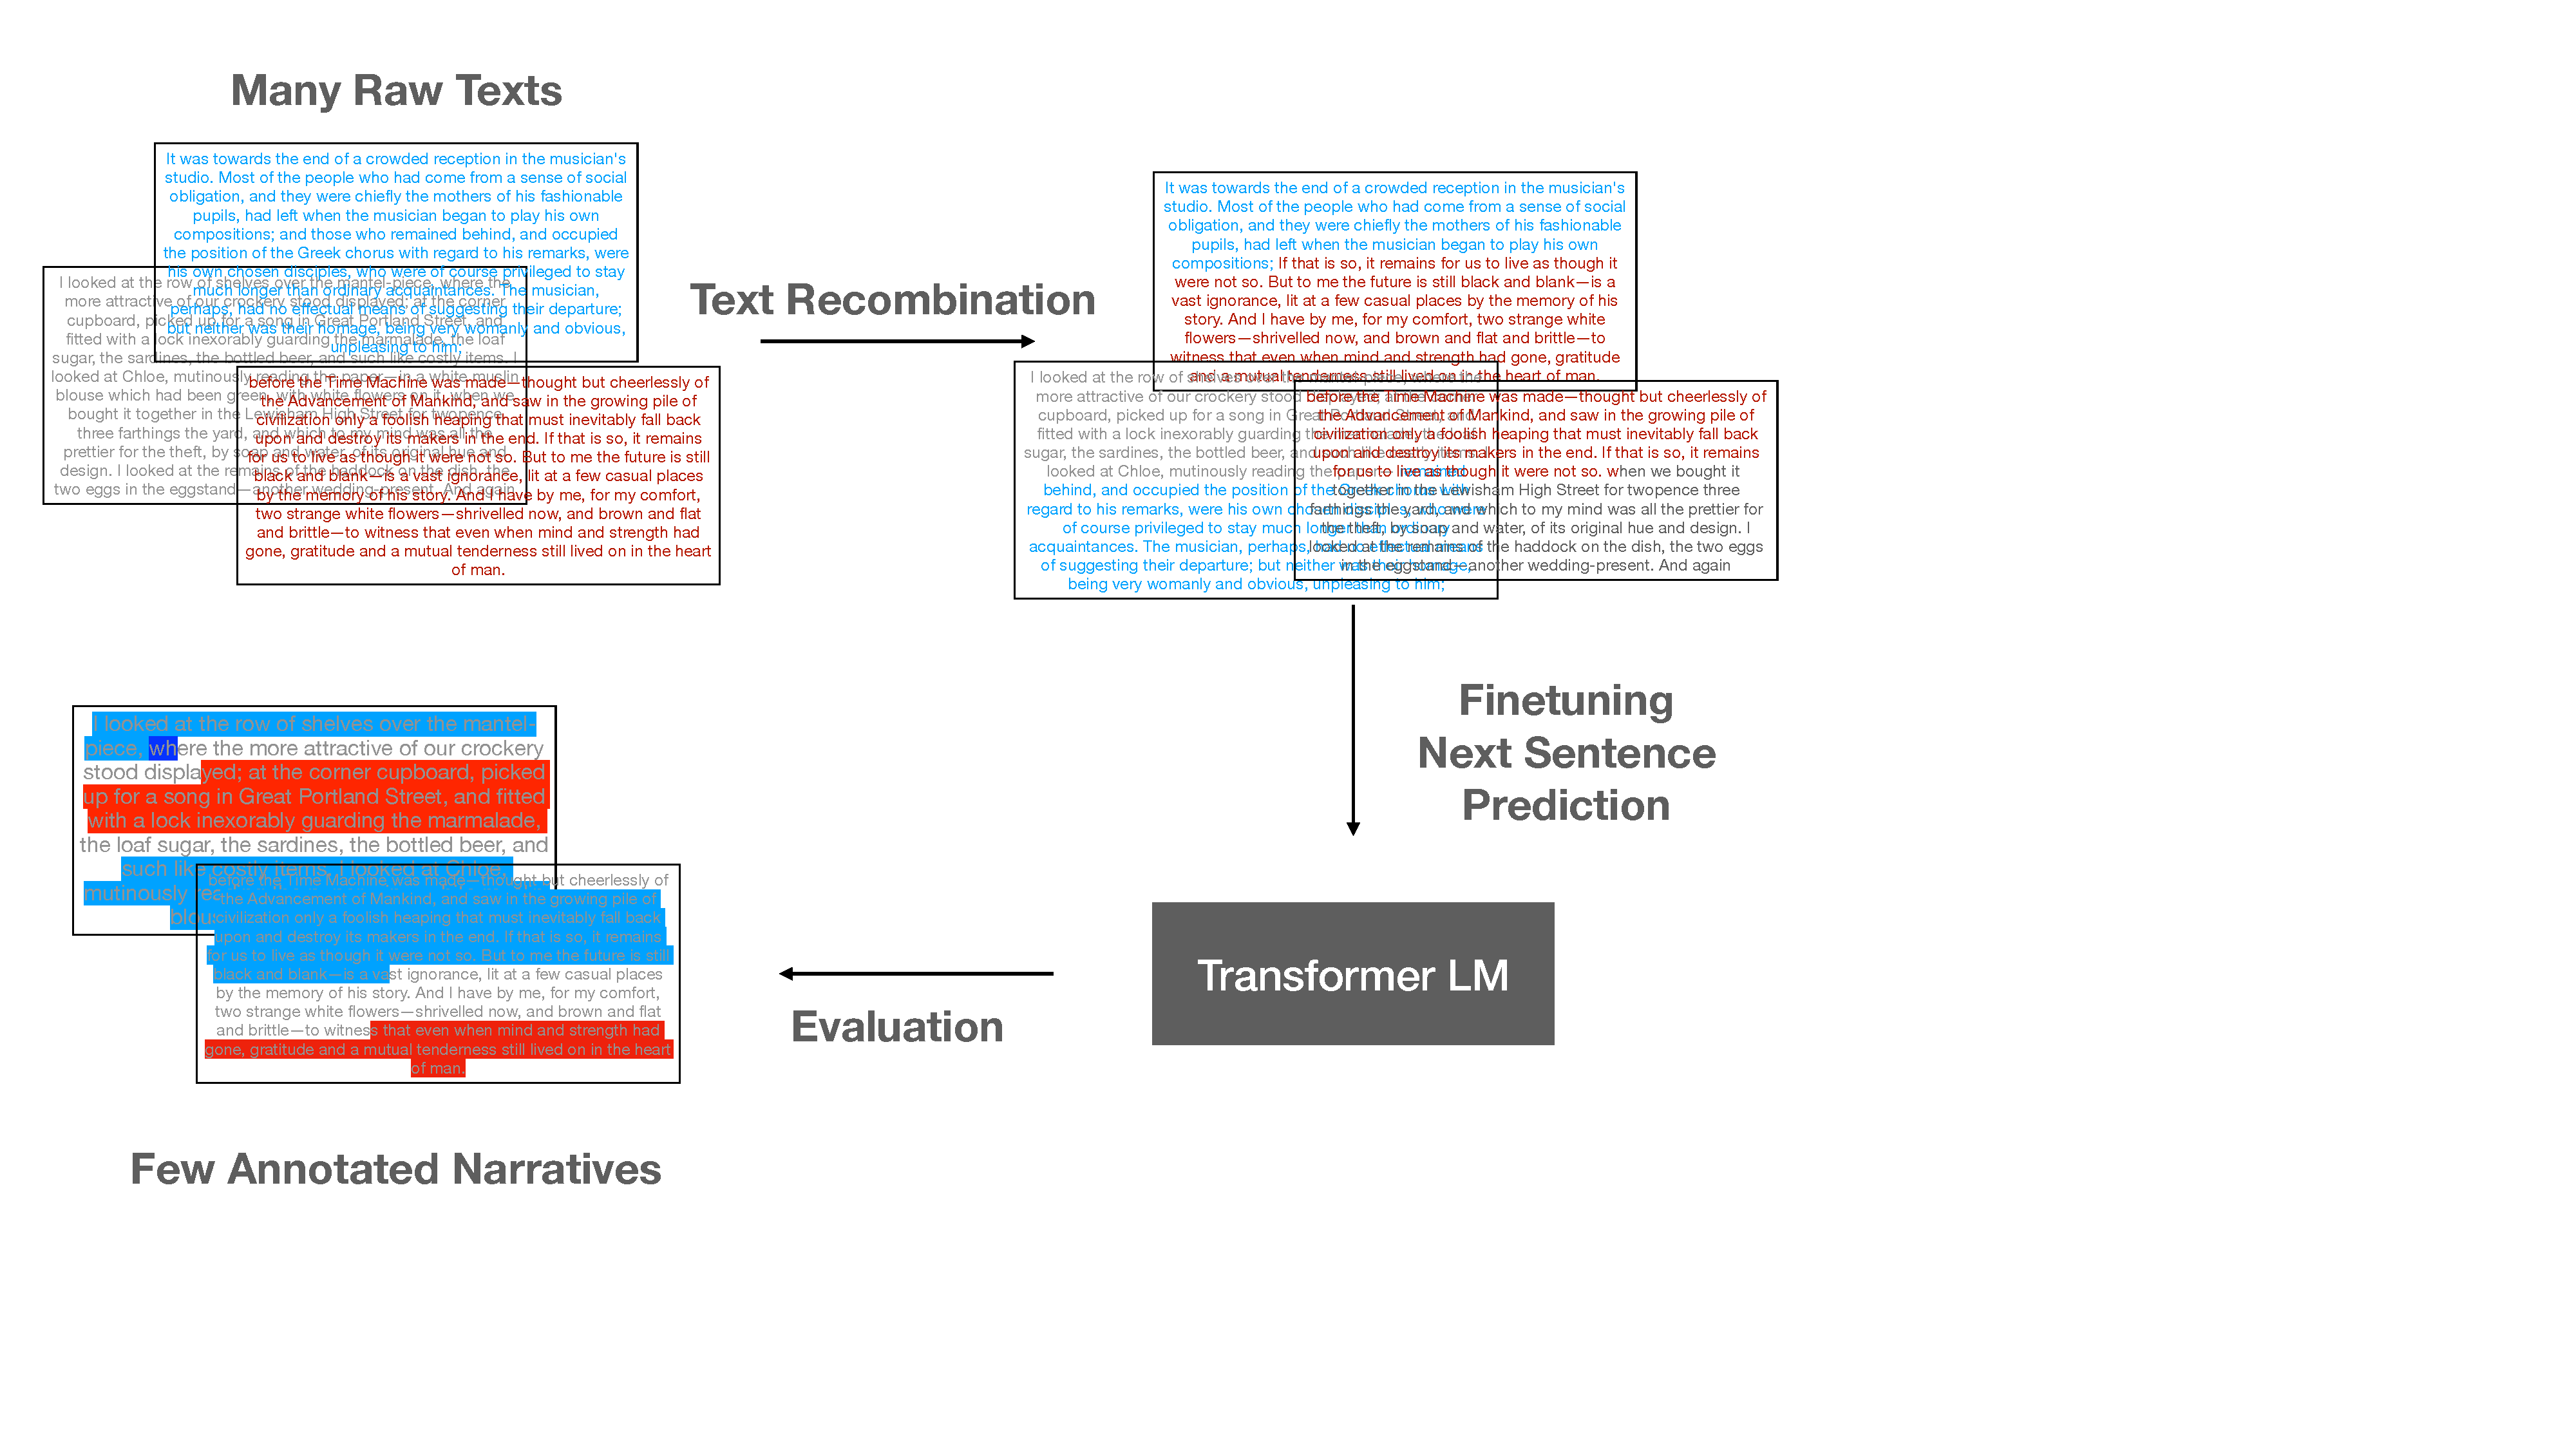
\includegraphics[width=0.45\paperwidth]{../paper/workflow.pdf}};
\end{tikzpicture}
\pause
\begin{columns}
\begin{column}{0.47\paperwidth}
\begin{block}{Experiments}
\setbeamertemplate{enumerate items}[circle]
\renewcommand\outlinei{enumerate}
\begin{outline}
\1 Evaluation on synthetic stories
\1 Evaluation on real level-annotated stories
\end{outline}
\end{block}  
\end{column}
\begin{column}{0.4\paperwidth}
  
\end{column}
\end{columns}
\end{frame}

\begin{frame}{Experiment 1: Evaluation on Synthetic Stories}
\begin{outline}
\1 Original BERT model provided by HuggingFace \inlineslidecite{devlin_bert_2019}
\1 Use next sentence prediction head for level boundary detection
\1 Evaluation with and without fine-tuning on synthetic data set
\1 Metrics: precision, recall, boundary similarity \inlineslidecite{Fournier:2013aa}
\2 Averaged over test set (\num{300} texts)
\2 Boundary similarity: Transposition window of $n_t=100$ characters
\1 \alert{Welches Kontextfenster haben wir hier genommen?}
\end{outline}
\pause
\begin{table}
  
\begin{tabular}{l
  S[table-format=2.2]@{\hspace{0em}}S[table-format=2.1,table-space-text-pre = $\pm$]
  S[table-format=2.2]@{\hspace{0em}}S[table-format=2.1,table-space-text-pre = $\pm$]
  S[table-format=2.2]@{\hspace{0em}}S[table-format=2.1,table-space-text-pre = $\pm$]}
\toprule
Finetuning & \multicolumn{2}{c}{Precision} & \multicolumn{2}{c}{Recall} & \multicolumn{2}{c}{Boundary sim.} \\
\midrule
No & 
2.61 & {$\pm$} 1.8 & 55.41 & {$\pm$} 25.2 & 2.51 & {$\pm$} 1.8 \\
Yes &
32.39 & {$\pm$} 36.09 & 25.68 & {$\pm$} 27.12 & 19.20 & {$\pm$} 24.25 \\
\bottomrule
\end{tabular}
\end{table}
\end{frame}

\begin{frame}{Experiment 2: Evaluation on Real Level-Annotated Stories}
\begin{outline}
\1 Re-use of guideline development shared task
\1 Evaluation on all annotations for all guidelines
\2 I.e.: 2 annotators for each of 7 guidelines
\1 With and without fine-tuning
\end{outline}

\begin{table}
\small
\begin{tabular}{lS[table-format=2.2]S[table-format=2.2]@{\hspace{4em}}S[table-format=2.2]S[table-format=2.2]@{\hspace{4em}}S[table-format=-2.2]S[table-format=-2.2]}
\toprule
 & \multicolumn{2}{l}{Without finetuning} &  \multicolumn{2}{l}{With finetuning} & \multicolumn{2}{l}{Gain by finetuning} \\
Guideline & {Precision} & {Recall} & {Precision} & {Recall} & {Precision} & {Recall} \\
\midrule

% \multirow{2}{*}{1} & 14.36 & 9.37 & 25.64 & 5.89 & 11.28 & -3.48\\
%   & 14.36 & 14.27 & 21.79 & 7.72 & 7.44 & -6.54\\
% \midrule
% \multirow{2}{*}{2} & 11.41 & 6.75 & 17.95 & 4.59 & 6.54 & -2.17\\
%   & 7.56 & 4.58 & 14.10 & 5.22 & 6.54 & 0.64\\
% \midrule
\multirow{2}{*}{\textcite{Ketschik2021On}} & 12.27 & 11.08 & 33.33 & 10.76 & 21.06 & -0.32\\
  & 7.69 & 7.13 & 10.26 & 2.98 & 2.56 & -4.15\\
\midrule
\multirow{2}{*}{\textcite{Barth2021Annotation}} & 12.18 & 9.79 & 17.95 & 7.40 & 5.77 & -2.39\\
  & 15.13 & 9.70 & 10.26 & 2.75 & -4.87 & -6.95\\
%\midrule
% \multirow{2}{*}{6} & 15.69 & 14.43 & 23.85 & 14.47 & 8.15 & 0.04\\
%   & 18.36 & 9.03 & 21.79 & 3.90 & 3.44 & -5.13\\
% \midrule
% \multirow{2}{*}{7} & 7.69 & 19.23 & 17.95 & 13.46 & 10.26 & -5.77\\
%   & 7.69 & 19.23 & 17.95 & 12.09 & 10.26 & -7.14\\
% \midrule
% \multirow{2}{*}{8} & 8.08 & 11.54 & 17.95 & 9.10 & 9.87 & -2.44\\
%   & 9.87 & 13.41 & 15.38 & 5.40 & 5.51 & -8.01\\
\bottomrule
\end{tabular}
\caption{Prediction results for narrative level boundaries (see paper for full table)}
\end{table}
\end{frame}

\begin{frame}{Conclusions and Outlook}
\begin{outline}
\1 Annotating narrative levels classically does not scale
\2 Mostly because it's a non-local phenomenon
\1 Even crudely generating training data helps
\end{outline}
\pause
\begin{block}{Outlook: Two-Track Shared Task on Narrative Level Detection}
\renewcommand\outlinei{enumerate}
\begin{outline}
\1 Training data generation
\2 Interdisciplinary audience: Computational (literary studies|linguistics), digital humanities, \dots 
\2 Better combinations by optimizing boundary contexts
\2 Evaluation: Performance of a baseline BERT system
\1 Automatic detection
\2 Computational linguistics audience
\2 Long text phenomenon
\2 Evaluation: Performance on properly annotated gold data
\end{outline}
\end{block}

\end{frame}


\begin{frame}[plain]
\begin{tikzpicture}[remember picture,overlay]
\node at (current page.center) {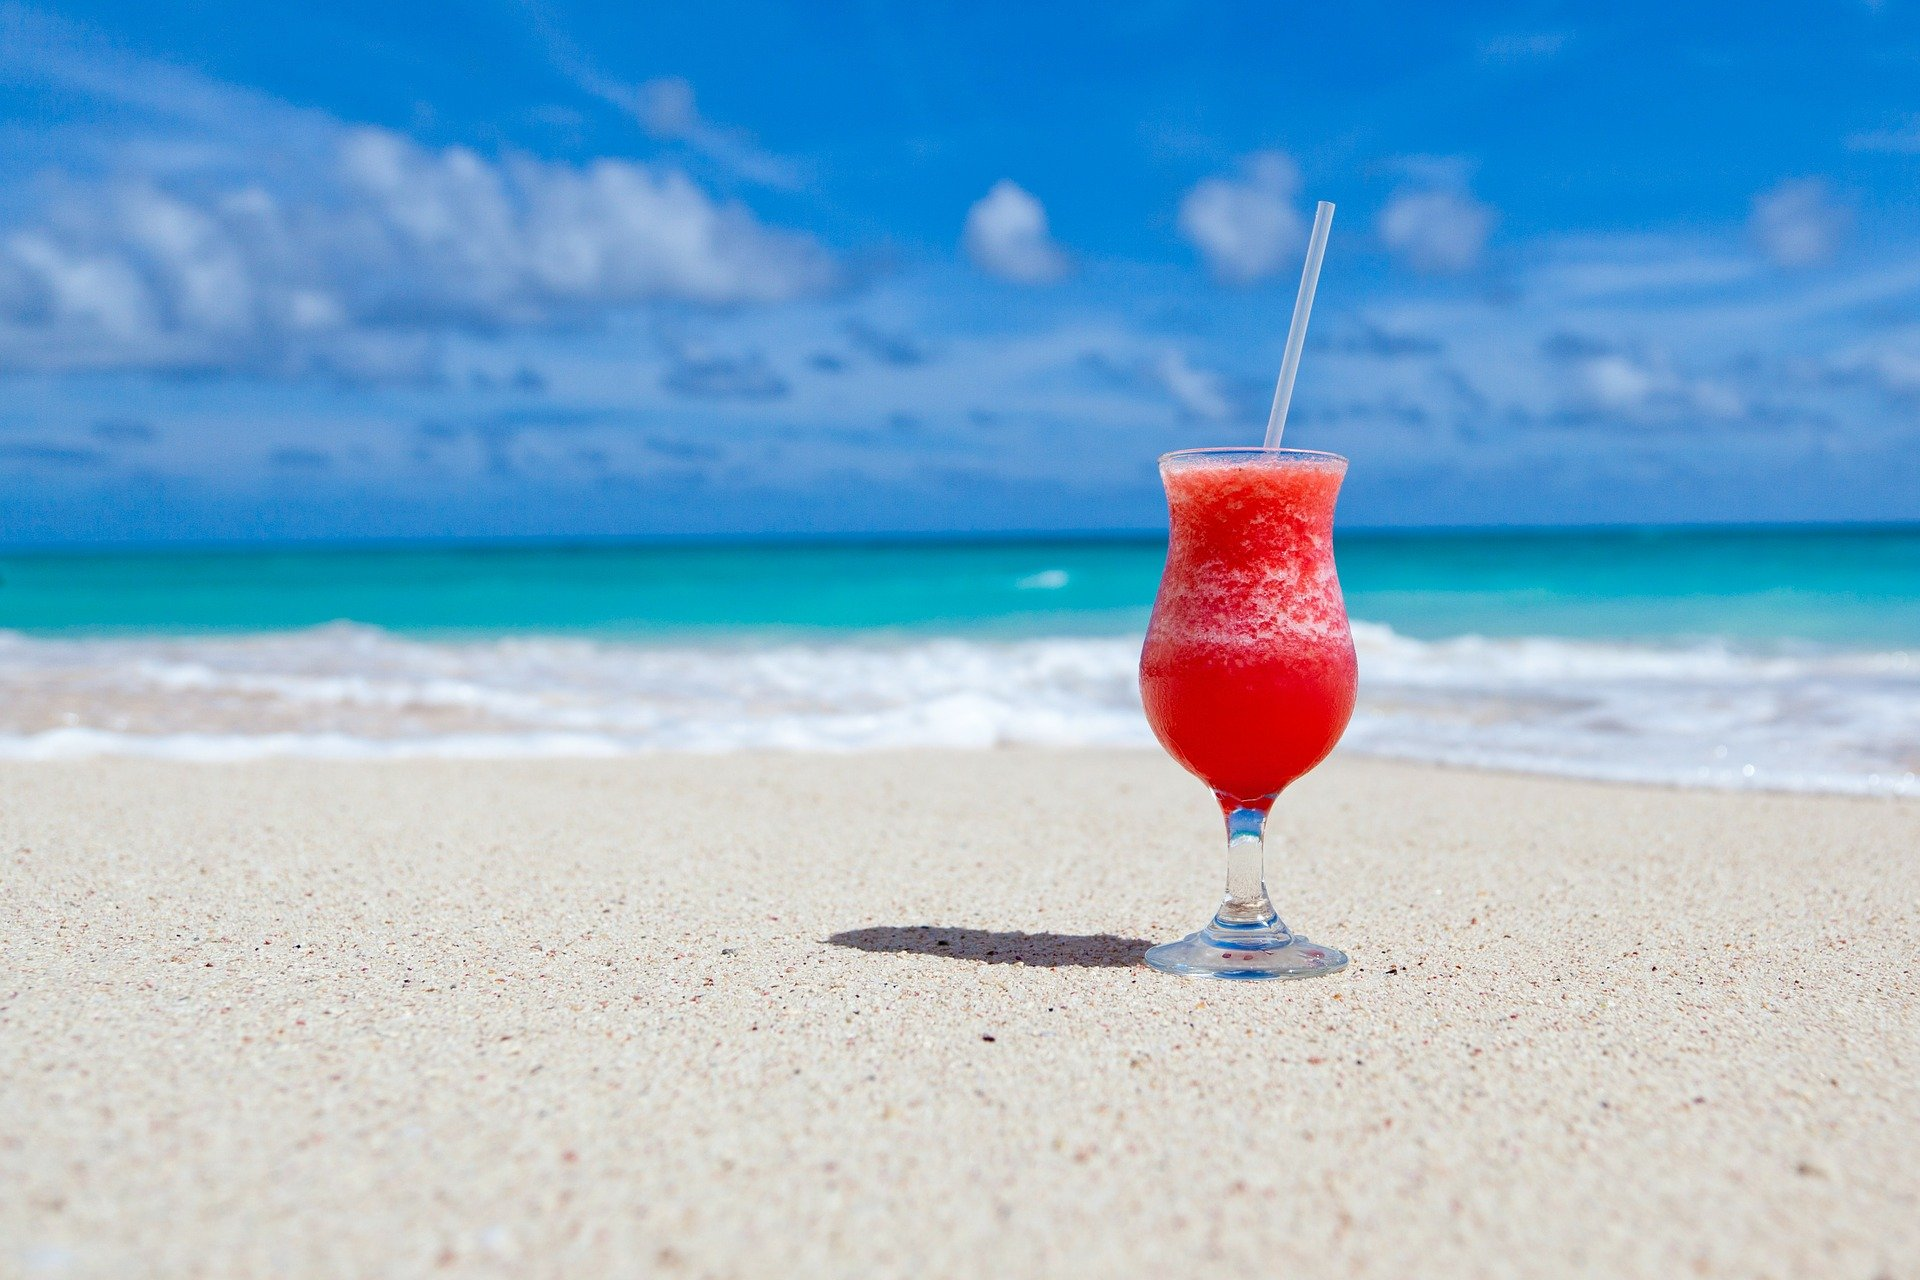
\includegraphics[width=\paperwidth]{drink-84533_1920.jpg}};
\node at (current page.center) [align=center,font=\LARGE\itshape,xshift=-3.5cm,yshift=-2.5cm] {Thank you!}; 
\end{tikzpicture}
\end{frame}

\appendix

\begin{frame}{Context Window}
\begin{figure}
\resizebox{\linewidth}{!}{
\begin{tikzpicture}
\coordinate (n10_54) at (0,0);
\coordinate (n10_154) at (0,-1.1);
\coordinate (n10_254) at (0,-2.2);
\node at (n10_54)  [anchor=east,font=\Large] {$c=54$};
\node at (n10_154) [anchor=east,font=\Large] {$c=154$};
\node at (n10_254) [anchor=east,font=\Large] {$c=254$};
\draw ($(n10_54)+(0,0)$)   -- ($(n10_54)+(0.01,0.62358475)$) 
  -- ($(n10_54)+(0.02,0)$) 
  -- ($(n10_54)+(0.03,0)$) 
  -- ($(n10_54)+(0.04,0)$) 
  -- ($(n10_54)+(0.05,0)$) 
  -- ($(n10_54)+(0.06,0)$) 
  -- ($(n10_54)+(0.07,0)$) 
  -- ($(n10_54)+(0.08,0)$) 
  -- ($(n10_54)+(0.09,0)$) 
  -- ($(n10_54)+(0.1,0)$) 
  -- ($(n10_54)+(0.11,0)$) 
  -- ($(n10_54)+(0.12,0)$) 
  -- ($(n10_54)+(0.13,0)$) 
  -- ($(n10_54)+(0.14,0)$) 
  -- ($(n10_54)+(0.15,0)$) 
  -- ($(n10_54)+(0.16,0)$) 
  -- ($(n10_54)+(0.17,0)$) 
  -- ($(n10_54)+(0.18,0)$) 
  -- ($(n10_54)+(0.19,0)$) 
  -- ($(n10_54)+(0.2,0)$) 
  -- ($(n10_54)+(0.21,0)$) 
  -- ($(n10_54)+(0.22,0)$) 
  -- ($(n10_54)+(0.23,0)$) 
  -- ($(n10_54)+(0.24,0)$) 
  -- ($(n10_54)+(0.25,0)$) 
  -- ($(n10_54)+(0.26,0)$) 
  -- ($(n10_54)+(0.27,0)$) 
  -- ($(n10_54)+(0.28,0)$) 
  -- ($(n10_54)+(0.29,0)$) 
  -- ($(n10_54)+(0.3,0)$) 
  -- ($(n10_54)+(0.31,0)$) 
  -- ($(n10_54)+(0.32,0)$) 
  -- ($(n10_54)+(0.33,0)$) 
  -- ($(n10_54)+(0.34,0)$) 
  -- ($(n10_54)+(0.35,0)$) 
  -- ($(n10_54)+(0.36,0)$) 
  -- ($(n10_54)+(0.37,0)$) 
  -- ($(n10_54)+(0.38,0)$) 
  -- ($(n10_54)+(0.39,0)$) 
  -- ($(n10_54)+(0.4,0)$) 
  -- ($(n10_54)+(0.41,0.1885348)$) 
  -- ($(n10_54)+(0.42,0)$) 
  -- ($(n10_54)+(0.43,0)$) 
  -- ($(n10_54)+(0.44,0)$) 
  -- ($(n10_54)+(0.45,0)$) 
  -- ($(n10_54)+(0.46,0)$) 
  -- ($(n10_54)+(0.47,0)$) 
  -- ($(n10_54)+(0.48,0)$) 
  -- ($(n10_54)+(0.49,0)$) 
  -- ($(n10_54)+(0.5,0)$) 
  -- ($(n10_54)+(0.51,0)$) 
  -- ($(n10_54)+(0.52,0)$) 
  -- ($(n10_54)+(0.53,0)$) 
  -- ($(n10_54)+(0.54,0)$) 
  -- ($(n10_54)+(0.55,0)$) 
  -- ($(n10_54)+(0.56,0)$) 
  -- ($(n10_54)+(0.57,0)$) 
  -- ($(n10_54)+(0.58,0)$) 
  -- ($(n10_54)+(0.59,0)$) 
  -- ($(n10_54)+(0.6,0)$) 
  -- ($(n10_54)+(0.61,0)$) 
  -- ($(n10_54)+(0.62,0)$) 
  -- ($(n10_54)+(0.63,0)$) 
  -- ($(n10_54)+(0.64,0)$) 
  -- ($(n10_54)+(0.65,0)$) 
  -- ($(n10_54)+(0.66,0)$) 
  -- ($(n10_54)+(0.67,0)$) 
  -- ($(n10_54)+(0.68,0)$) 
  -- ($(n10_54)+(0.69,0)$) 
  -- ($(n10_54)+(0.7,0)$) 
  -- ($(n10_54)+(0.71,0)$) 
  -- ($(n10_54)+(0.72,0)$) 
  -- ($(n10_54)+(0.73,0)$) 
  -- ($(n10_54)+(0.74,0)$) 
  -- ($(n10_54)+(0.75,0)$) 
  -- ($(n10_54)+(0.76,0)$) 
  -- ($(n10_54)+(0.77,0)$) 
  -- ($(n10_54)+(0.78,0)$) 
  -- ($(n10_54)+(0.79,0)$) 
  -- ($(n10_54)+(0.8,0)$) 
  -- ($(n10_54)+(0.81,0)$) 
  -- ($(n10_54)+(0.82,0)$) 
  -- ($(n10_54)+(0.83,0)$) 
  -- ($(n10_54)+(0.84,0)$) 
  -- ($(n10_54)+(0.85,0)$) 
  -- ($(n10_54)+(0.86,0)$) 
  -- ($(n10_54)+(0.87,0)$) 
  -- ($(n10_54)+(0.88,0)$) 
  -- ($(n10_54)+(0.89,0)$) 
  -- ($(n10_54)+(0.9,0)$) 
  -- ($(n10_54)+(0.91,0)$) 
  -- ($(n10_54)+(0.92,0)$) 
  -- ($(n10_54)+(0.93,0)$) 
  -- ($(n10_54)+(0.94,0)$) 
  -- ($(n10_54)+(0.95,0)$) 
  -- ($(n10_54)+(0.96,0)$) 
  -- ($(n10_54)+(0.97,0)$) 
  -- ($(n10_54)+(0.98,0)$) 
  -- ($(n10_54)+(0.99,0)$) 
  -- ($(n10_54)+(1.0,0)$) 
  -- ($(n10_54)+(1.01,0)$) 
  -- ($(n10_54)+(1.02,0)$) 
  -- ($(n10_54)+(1.03,0)$) 
  -- ($(n10_54)+(1.04,0)$) 
  -- ($(n10_54)+(1.05,0)$) 
  -- ($(n10_54)+(1.06,0)$) 
  -- ($(n10_54)+(1.07,0)$) 
  -- ($(n10_54)+(1.08,0)$) 
  -- ($(n10_54)+(1.09,0)$) 
  -- ($(n10_54)+(1.1,0)$) 
  -- ($(n10_54)+(1.11,0)$) 
  -- ($(n10_54)+(1.12,0)$) 
  -- ($(n10_54)+(1.13,0)$) 
  -- ($(n10_54)+(1.14,0)$) 
  -- ($(n10_54)+(1.15,0)$) 
  -- ($(n10_54)+(1.16,0)$) 
  -- ($(n10_54)+(1.17,0)$) 
  -- ($(n10_54)+(1.18,0.9972614)$) 
  -- ($(n10_54)+(1.19,0.01675403)$) 
  -- ($(n10_54)+(1.2,0.99983537)$) 
  -- ($(n10_54)+(1.21,0)$) 
  -- ($(n10_54)+(1.22,0)$) 
  -- ($(n10_54)+(1.23,0)$) 
  -- ($(n10_54)+(1.24,0)$) 
  -- ($(n10_54)+(1.25,0)$) 
  -- ($(n10_54)+(1.26,0)$) 
  -- ($(n10_54)+(1.27,0)$) 
  -- ($(n10_54)+(1.28,0)$) 
  -- ($(n10_54)+(1.29,0.9912443)$) 
  -- ($(n10_54)+(1.3,0)$) 
  -- ($(n10_54)+(1.31,0.9785751)$) 
  -- ($(n10_54)+(1.32,0)$) 
  -- ($(n10_54)+(1.33,0)$) 
  -- ($(n10_54)+(1.34,0)$) 
  -- ($(n10_54)+(1.35,0.0697996)$) 
  -- ($(n10_54)+(1.36,0)$) 
  -- ($(n10_54)+(1.37,0)$) 
  -- ($(n10_54)+(1.38,0)$) 
  -- ($(n10_54)+(1.39,0)$) 
  -- ($(n10_54)+(1.4,0)$) 
  -- ($(n10_54)+(1.41,0)$) 
  -- ($(n10_54)+(1.42,0)$) 
  -- ($(n10_54)+(1.43,0)$) 
  -- ($(n10_54)+(1.44,0)$) 
  -- ($(n10_54)+(1.45,0)$) 
  -- ($(n10_54)+(1.46,0)$) 
  -- ($(n10_54)+(1.47,0)$) 
  -- ($(n10_54)+(1.48,0)$) 
  -- ($(n10_54)+(1.49,0.99719894)$) 
  -- ($(n10_54)+(1.5,0)$) 
  -- ($(n10_54)+(1.51,0)$) 
  -- ($(n10_54)+(1.52,0)$) 
  -- ($(n10_54)+(1.53,0)$) 
  -- ($(n10_54)+(1.54,0)$) 
  -- ($(n10_54)+(1.55,0)$) 
  -- ($(n10_54)+(1.56,0)$) 
  -- ($(n10_54)+(1.57,0)$) 
  -- ($(n10_54)+(1.58,0)$) 
  -- ($(n10_54)+(1.59,0)$) 
  -- ($(n10_54)+(1.6,0)$) 
  -- ($(n10_54)+(1.61,0)$) 
  -- ($(n10_54)+(1.62,0)$) 
  -- ($(n10_54)+(1.63,0)$) 
  -- ($(n10_54)+(1.64,0)$) 
  -- ($(n10_54)+(1.65,0)$) 
  -- ($(n10_54)+(1.66,0)$) 
  -- ($(n10_54)+(1.67,0)$) 
  -- ($(n10_54)+(1.68,0)$) 
  -- ($(n10_54)+(1.69,0)$) 
  -- ($(n10_54)+(1.7,0)$) 
  -- ($(n10_54)+(1.71,0)$) 
  -- ($(n10_54)+(1.72,0)$) 
  -- ($(n10_54)+(1.73,0)$) 
  -- ($(n10_54)+(1.74,0)$) 
  -- ($(n10_54)+(1.75,0)$) 
  -- ($(n10_54)+(1.76,0)$) 
  -- ($(n10_54)+(1.77,0)$) 
  -- ($(n10_54)+(1.78,0)$) 
  -- ($(n10_54)+(1.79,0)$) 
  -- ($(n10_54)+(1.8,0)$) 
  -- ($(n10_54)+(1.81,0)$) 
  -- ($(n10_54)+(1.82,0)$) 
  -- ($(n10_54)+(1.83,0)$) 
  -- ($(n10_54)+(1.84,0)$) 
  -- ($(n10_54)+(1.85,0)$) 
  -- ($(n10_54)+(1.86,0)$) 
  -- ($(n10_54)+(1.87,0)$) 
  -- ($(n10_54)+(1.88,0)$) 
  -- ($(n10_54)+(1.89,0.9990088)$) 
  -- ($(n10_54)+(1.9,0)$) 
  -- ($(n10_54)+(1.91,0)$) 
  -- ($(n10_54)+(1.92,0)$) 
  -- ($(n10_54)+(1.93,0)$) 
  -- ($(n10_54)+(1.94,0)$) 
  -- ($(n10_54)+(1.95,0)$) 
  -- ($(n10_54)+(1.96,0)$) 
  -- ($(n10_54)+(1.97,0)$) 
  -- ($(n10_54)+(1.98,0)$) 
  -- ($(n10_54)+(1.99,0)$) 
  -- ($(n10_54)+(2.0,0)$) 
  -- ($(n10_54)+(2.01,0)$) 
  -- ($(n10_54)+(2.02,0)$) 
  -- ($(n10_54)+(2.03,0)$) 
  -- ($(n10_54)+(2.04,0)$) 
  -- ($(n10_54)+(2.05,0)$) 
  -- ($(n10_54)+(2.06,0)$) 
  -- ($(n10_54)+(2.07,0)$) 
  -- ($(n10_54)+(2.08,0)$) 
  -- ($(n10_54)+(2.09,0)$) 
  -- ($(n10_54)+(2.1,0)$) 
  -- ($(n10_54)+(2.11,0)$) 
  -- ($(n10_54)+(2.12,0)$) 
  -- ($(n10_54)+(2.13,0)$) 
  -- ($(n10_54)+(2.14,0)$) 
  -- ($(n10_54)+(2.15,0)$) 
  -- ($(n10_54)+(2.16,0)$) 
  -- ($(n10_54)+(2.17,0)$) 
  -- ($(n10_54)+(2.18,0)$) 
  -- ($(n10_54)+(2.19,0)$) 
  -- ($(n10_54)+(2.2,0)$) 
  -- ($(n10_54)+(2.21,0)$) 
  -- ($(n10_54)+(2.22,0)$) 
  -- ($(n10_54)+(2.23,0)$) 
  -- ($(n10_54)+(2.24,0)$) 
  -- ($(n10_54)+(2.25,0)$) 
  -- ($(n10_54)+(2.26,0)$) 
  -- ($(n10_54)+(2.27,0)$) 
  -- ($(n10_54)+(2.28,0)$) 
  -- ($(n10_54)+(2.29,0)$) 
  -- ($(n10_54)+(2.3,0)$) 
  -- ($(n10_54)+(2.31,0)$) 
  -- ($(n10_54)+(2.32,0)$) 
  -- ($(n10_54)+(2.33,0)$) 
  -- ($(n10_54)+(2.34,0)$) 
  -- ($(n10_54)+(2.35,0)$) 
  -- ($(n10_54)+(2.36,0)$) 
  -- ($(n10_54)+(2.37,0)$) 
  -- ($(n10_54)+(2.38,0)$) 
  -- ($(n10_54)+(2.39,0)$) 
  -- ($(n10_54)+(2.4,0)$) 
  -- ($(n10_54)+(2.41,0)$) 
  -- ($(n10_54)+(2.42,0)$) 
  -- ($(n10_54)+(2.43,0)$) 
  -- ($(n10_54)+(2.44,0)$) 
  -- ($(n10_54)+(2.45,0)$) 
  -- ($(n10_54)+(2.46,0)$) 
  -- ($(n10_54)+(2.47,0)$) 
  -- ($(n10_54)+(2.48,0)$) 
  -- ($(n10_54)+(2.49,0)$) 
  -- ($(n10_54)+(2.5,0)$) 
  -- ($(n10_54)+(2.51,0)$) 
  -- ($(n10_54)+(2.52,0)$) 
  -- ($(n10_54)+(2.53,0)$) 
  -- ($(n10_54)+(2.54,0)$) 
  -- ($(n10_54)+(2.55,0)$) 
  -- ($(n10_54)+(2.56,0)$) 
  -- ($(n10_54)+(2.57,0)$) 
  -- ($(n10_54)+(2.58,0)$) 
  -- ($(n10_54)+(2.59,0)$) 
  -- ($(n10_54)+(2.6,0)$) 
  -- ($(n10_54)+(2.61,0)$) 
  -- ($(n10_54)+(2.62,0)$) 
  -- ($(n10_54)+(2.63,0)$) 
  -- ($(n10_54)+(2.64,0)$) 
  -- ($(n10_54)+(2.65,0)$) 
  -- ($(n10_54)+(2.66,0)$) 
  -- ($(n10_54)+(2.67,0)$) 
  -- ($(n10_54)+(2.68,0)$) 
  -- ($(n10_54)+(2.69,0)$) 
  -- ($(n10_54)+(2.7,0)$) 
  -- ($(n10_54)+(2.71,0.04828244)$) 
  -- ($(n10_54)+(2.72,0)$) 
  -- ($(n10_54)+(2.73,0)$) 
  -- ($(n10_54)+(2.74,0)$) 
  -- ($(n10_54)+(2.75,0)$) 
  -- ($(n10_54)+(2.76,0)$) 
  -- ($(n10_54)+(2.77,0)$) 
  -- ($(n10_54)+(2.78,0)$) 
  -- ($(n10_54)+(2.79,0)$) 
  -- ($(n10_54)+(2.8,0)$) 
  -- ($(n10_54)+(2.81,0)$) 
  -- ($(n10_54)+(2.82,0)$) 
  -- ($(n10_54)+(2.83,0)$) 
  -- ($(n10_54)+(2.84,0)$) 
  -- ($(n10_54)+(2.85,0)$) 
  -- ($(n10_54)+(2.86,0)$) 
  -- ($(n10_54)+(2.87,0)$) 
  -- ($(n10_54)+(2.88,0)$) 
  -- ($(n10_54)+(2.89,0)$) 
  -- ($(n10_54)+(2.9,0)$) 
  -- ($(n10_54)+(2.91,0)$) 
  -- ($(n10_54)+(2.92,0)$) 
  -- ($(n10_54)+(2.93,0)$) 
  -- ($(n10_54)+(2.94,0)$) 
  -- ($(n10_54)+(2.95,0)$) 
  -- ($(n10_54)+(2.96,0)$) 
  -- ($(n10_54)+(2.97,0)$) 
  -- ($(n10_54)+(2.98,0)$) 
  -- ($(n10_54)+(2.99,0)$) 
  -- ($(n10_54)+(3.0,0)$) 
  -- ($(n10_54)+(3.01,0)$) 
  -- ($(n10_54)+(3.02,0.04562347)$) 
  -- ($(n10_54)+(3.03,0)$) 
  -- ($(n10_54)+(3.04,0)$) 
  -- ($(n10_54)+(3.05,0)$) 
  -- ($(n10_54)+(3.06,0)$) 
  -- ($(n10_54)+(3.07,0)$) 
  -- ($(n10_54)+(3.08,0)$) 
  -- ($(n10_54)+(3.09,0)$) 
  -- ($(n10_54)+(3.1,0)$) 
  -- ($(n10_54)+(3.11,0)$) 
  -- ($(n10_54)+(3.12,0)$) 
  -- ($(n10_54)+(3.13,0)$) 
  -- ($(n10_54)+(3.14,0)$) 
  -- ($(n10_54)+(3.15,0)$) 
  -- ($(n10_54)+(3.16,0)$) 
  -- ($(n10_54)+(3.17,0)$) 
  -- ($(n10_54)+(3.18,0)$) 
  -- ($(n10_54)+(3.19,0)$) 
  -- ($(n10_54)+(3.2,0)$) 
  -- ($(n10_54)+(3.21,0)$) 
  -- ($(n10_54)+(3.22,0)$) 
  -- ($(n10_54)+(3.23,0)$) 
  -- ($(n10_54)+(3.24,0)$) 
  -- ($(n10_54)+(3.25,0)$) 
  -- ($(n10_54)+(3.26,0)$) 
  -- ($(n10_54)+(3.27,0)$) 
  -- ($(n10_54)+(3.28,0)$) 
  -- ($(n10_54)+(3.29,0)$) 
  -- ($(n10_54)+(3.3,0)$) 
  -- ($(n10_54)+(3.31,0)$) 
  -- ($(n10_54)+(3.32,0)$) 
  -- ($(n10_54)+(3.33,0)$) 
  -- ($(n10_54)+(3.34,0)$) 
  -- ($(n10_54)+(3.35,0)$) 
  -- ($(n10_54)+(3.36,0.9766258)$) 
  -- ($(n10_54)+(3.37,0.01238419)$) 
  -- ($(n10_54)+(3.38,0)$) 
  -- ($(n10_54)+(3.39,0)$) 
  -- ($(n10_54)+(3.4,0)$) 
  -- ($(n10_54)+(3.41,0)$) 
  -- ($(n10_54)+(3.42,0)$) 
  -- ($(n10_54)+(3.43,0)$) 
  -- ($(n10_54)+(3.44,0)$) 
  -- ($(n10_54)+(3.45,0)$) 
  -- ($(n10_54)+(3.46,0.99568605)$) 
  -- ($(n10_54)+(3.47,0)$) 
  -- ($(n10_54)+(3.48,0)$) 
  -- ($(n10_54)+(3.49,0)$) 
  -- ($(n10_54)+(3.5,0)$) 
  -- ($(n10_54)+(3.51,0)$) 
  -- ($(n10_54)+(3.52,0)$) 
  -- ($(n10_54)+(3.53,0)$) 
  -- ($(n10_54)+(3.54,0)$) 
  -- ($(n10_54)+(3.55,0)$) 
  -- ($(n10_54)+(3.56,0)$) 
  -- ($(n10_54)+(3.57,0)$) 
  -- ($(n10_54)+(3.58,0)$) 
  -- ($(n10_54)+(3.59,0)$) 
  -- ($(n10_54)+(3.6,0)$) 
  -- ($(n10_54)+(3.61,0)$) 
  -- ($(n10_54)+(3.62,0)$) 
  -- ($(n10_54)+(3.63,0)$) 
  -- ($(n10_54)+(3.64,0.01022508)$) 
  -- ($(n10_54)+(3.65,0.5548506)$) 
  -- ($(n10_54)+(3.66,0)$) 
  -- ($(n10_54)+(3.67,0)$) 
  -- ($(n10_54)+(3.68,0)$) 
  -- ($(n10_54)+(3.69,0)$) 
  -- ($(n10_54)+(3.7,0)$) 
  -- ($(n10_54)+(3.71,0)$) 
  -- ($(n10_54)+(3.72,0)$) 
  -- ($(n10_54)+(3.73,0)$) 
  -- ($(n10_54)+(3.74,0)$) 
  -- ($(n10_54)+(3.75,0)$) 
  -- ($(n10_54)+(3.76,0)$) 
  -- ($(n10_54)+(3.77,0)$) 
  -- ($(n10_54)+(3.78,0)$) 
  -- ($(n10_54)+(3.79,0)$) 
  -- ($(n10_54)+(3.8,0)$) 
  -- ($(n10_54)+(3.81,0)$) 
  -- ($(n10_54)+(3.82,0)$) 
  -- ($(n10_54)+(3.83,0)$) 
  -- ($(n10_54)+(3.84,0)$) 
  -- ($(n10_54)+(3.85,0)$) 
  -- ($(n10_54)+(3.86,0)$) 
  -- ($(n10_54)+(3.87,0)$) 
  -- ($(n10_54)+(3.88,0.8307729)$) 
  -- ($(n10_54)+(3.89,0)$) 
  -- ($(n10_54)+(3.9,0)$) 
  -- ($(n10_54)+(3.91,0)$) 
  -- ($(n10_54)+(3.92,0)$) 
  -- ($(n10_54)+(3.93,0)$) 
  -- ($(n10_54)+(3.94,0)$) 
  -- ($(n10_54)+(3.95,0)$) 
  -- ($(n10_54)+(3.96,0)$) 
  -- ($(n10_54)+(3.97,0)$) 
  -- ($(n10_54)+(3.98,0)$) 
  -- ($(n10_54)+(3.99,0)$) 
  -- ($(n10_54)+(4.0,0)$) 
  -- ($(n10_54)+(4.01,0)$) 
  -- ($(n10_54)+(4.02,0)$) 
  -- ($(n10_54)+(4.03,0)$) 
  -- ($(n10_54)+(4.04,0)$) 
  -- ($(n10_54)+(4.05,0.98726475)$) 
  -- ($(n10_54)+(4.06,0)$) 
  -- ($(n10_54)+(4.07,0)$) 
  -- ($(n10_54)+(4.08,0)$) 
  -- ($(n10_54)+(4.09,0)$) 
  -- ($(n10_54)+(4.1,0)$) 
  -- ($(n10_54)+(4.11,0.99935728)$) 
  -- ($(n10_54)+(4.12,0)$) 
  -- ($(n10_54)+(4.13,0)$) 
  -- ($(n10_54)+(4.14,0)$) 
  -- ($(n10_54)+(4.15,0)$) 
  -- ($(n10_54)+(4.16,0)$) 
  -- ($(n10_54)+(4.17,0)$) 
  -- ($(n10_54)+(4.18,0)$) 
  -- ($(n10_54)+(4.19,0)$) 
  -- ($(n10_54)+(4.2,0)$) 
  -- ($(n10_54)+(4.21,0)$) 
  -- ($(n10_54)+(4.22,0)$) 
  -- ($(n10_54)+(4.23,0)$) 
  -- ($(n10_54)+(4.24,0)$) 
  -- ($(n10_54)+(4.25,0)$) 
  -- ($(n10_54)+(4.26,0)$) 
  -- ($(n10_54)+(4.27,0)$) 
  -- ($(n10_54)+(4.28,0)$) 
  -- ($(n10_54)+(4.29,0)$) 
  -- ($(n10_54)+(4.3,0)$) 
  -- ($(n10_54)+(4.31,0)$) 
  -- ($(n10_54)+(4.32,0.95641404)$) 
  -- ($(n10_54)+(4.33,0)$) 
  -- ($(n10_54)+(4.34,0)$) 
  -- ($(n10_54)+(4.35,0)$) 
  -- ($(n10_54)+(4.36,0)$) 
  -- ($(n10_54)+(4.37,0)$) 
  -- ($(n10_54)+(4.38,0)$) 
  -- ($(n10_54)+(4.39,0)$) 
  -- ($(n10_54)+(4.4,0)$) 
  -- ($(n10_54)+(4.41,0)$) 
  -- ($(n10_54)+(4.42,0)$) 
  -- ($(n10_54)+(4.43,0)$) 
  -- ($(n10_54)+(4.44,0)$) 
  -- ($(n10_54)+(4.45,0)$) 
  -- ($(n10_54)+(4.46,0)$) 
  -- ($(n10_54)+(4.47,0)$) 
  -- ($(n10_54)+(4.48,0)$) 
  -- ($(n10_54)+(4.49,0.99977762)$) 
  -- ($(n10_54)+(4.5,0)$) 
  -- ($(n10_54)+(4.51,0)$) 
  -- ($(n10_54)+(4.52,0)$) 
  -- ($(n10_54)+(4.53,0)$) 
  -- ($(n10_54)+(4.54,0)$) 
  -- ($(n10_54)+(4.55,0)$) 
  -- ($(n10_54)+(4.56,0)$) 
  -- ($(n10_54)+(4.57,0)$) 
  -- ($(n10_54)+(4.58,0)$) 
  -- ($(n10_54)+(4.59,0)$) 
  -- ($(n10_54)+(4.6,0)$) 
  -- ($(n10_54)+(4.61,0)$) 
  -- ($(n10_54)+(4.62,0)$) 
  -- ($(n10_54)+(4.63,0)$) 
  -- ($(n10_54)+(4.64,0)$) 
  -- ($(n10_54)+(4.65,0)$) 
  -- ($(n10_54)+(4.66,0)$) 
  -- ($(n10_54)+(4.67,0)$) 
  -- ($(n10_54)+(4.68,0)$) 
  -- ($(n10_54)+(4.69,0)$) 
  -- ($(n10_54)+(4.7,0)$) 
  -- ($(n10_54)+(4.71,0.03246698)$) 
  -- ($(n10_54)+(4.72,0)$) 
  -- ($(n10_54)+(4.73,0)$) 
  -- ($(n10_54)+(4.74,0)$) 
  -- ($(n10_54)+(4.75,0)$) 
  -- ($(n10_54)+(4.76,0)$) 
  -- ($(n10_54)+(4.77,0)$) 
  -- ($(n10_54)+(4.78,0)$) 
  -- ($(n10_54)+(4.79,0)$) 
  -- ($(n10_54)+(4.8,0)$) 
  -- ($(n10_54)+(4.81,0.9984054)$) 
  -- ($(n10_54)+(4.82,0)$) 
  -- ($(n10_54)+(4.83,0)$) 
  -- ($(n10_54)+(4.84,0)$) 
  -- ($(n10_54)+(4.85,0.9986817)$) 
  -- ($(n10_54)+(4.86,0.9925051)$) 
  -- ($(n10_54)+(4.87,0)$) 
  -- ($(n10_54)+(4.88,0)$) 
  -- ($(n10_54)+(4.89,0)$) 
  -- ($(n10_54)+(4.9,0)$) 
  -- ($(n10_54)+(4.91,0)$) 
  -- ($(n10_54)+(4.92,0)$) 
  -- ($(n10_54)+(4.93,0)$) 
  -- ($(n10_54)+(4.94,0)$) 
  -- ($(n10_54)+(4.95,0)$) 
  -- ($(n10_54)+(4.96,0.99497175)$) 
  -- ($(n10_54)+(4.97,0)$) 
  -- ($(n10_54)+(4.98,0)$) 
  -- ($(n10_54)+(4.99,0)$) 
  -- ($(n10_54)+(5.0,0)$) 
  -- ($(n10_54)+(5.01,0)$) 
  -- ($(n10_54)+(5.02,0)$) 
  -- ($(n10_54)+(5.03,0)$) 
  -- ($(n10_54)+(5.04,0)$) 
  -- ($(n10_54)+(5.05,0)$) 
  -- ($(n10_54)+(5.06,0)$) 
  -- ($(n10_54)+(5.07,0)$) 
  -- ($(n10_54)+(5.08,0)$) 
  -- ($(n10_54)+(5.09,0)$) 
  -- ($(n10_54)+(5.1,0)$) 
  -- ($(n10_54)+(5.11,0)$) 
  -- ($(n10_54)+(5.12,0)$) 
  -- ($(n10_54)+(5.13,0)$) 
  -- ($(n10_54)+(5.14,0)$) 
  -- ($(n10_54)+(5.15,0.9621893)$) 
  -- ($(n10_54)+(5.16,0)$) 
  -- ($(n10_54)+(5.17,0)$) 
  -- ($(n10_54)+(5.18,0)$) 
  -- ($(n10_54)+(5.19,0)$) 
  -- ($(n10_54)+(5.2,0)$) 
  -- ($(n10_54)+(5.21,0)$) 
  -- ($(n10_54)+(5.22,0)$) 
  -- ($(n10_54)+(5.23,0)$) 
  -- ($(n10_54)+(5.24,0)$) 
  -- ($(n10_54)+(5.25,0)$) 
  -- ($(n10_54)+(5.26,0)$) 
  -- ($(n10_54)+(5.27,0)$) 
  -- ($(n10_54)+(5.28,0)$) 
  -- ($(n10_54)+(5.29,0.622788)$) 
  -- ($(n10_54)+(5.3,0)$) 
  -- ($(n10_54)+(5.31,0)$) 
  -- ($(n10_54)+(5.32,0)$) 
  -- ($(n10_54)+(5.33,0)$) 
  -- ($(n10_54)+(5.34,0)$) 
  -- ($(n10_54)+(5.35,0)$) 
  -- ($(n10_54)+(5.36,0)$) 
  -- ($(n10_54)+(5.37,0)$) 
  -- ($(n10_54)+(5.38,0)$) 
  -- ($(n10_54)+(5.39,0)$) 
  -- ($(n10_54)+(5.4,0)$) 
  -- ($(n10_54)+(5.41,0)$) 
  -- ($(n10_54)+(5.42,0)$) 
  -- ($(n10_54)+(5.43,0)$) 
  -- ($(n10_54)+(5.44,0)$) 
  -- ($(n10_54)+(5.45,0)$) 
  -- ($(n10_54)+(5.46,0)$) 
  -- ($(n10_54)+(5.47,0)$) 
  -- ($(n10_54)+(5.48,0)$) 
  -- ($(n10_54)+(5.49,0)$) 
  -- ($(n10_54)+(5.5,0)$) 
  -- ($(n10_54)+(5.51,0)$) 
  -- ($(n10_54)+(5.52,0)$) 
  -- ($(n10_54)+(5.53,0)$) 
  -- ($(n10_54)+(5.54,0)$) 
  -- ($(n10_54)+(5.55,0)$) 
  -- ($(n10_54)+(5.56,0)$) 
  -- ($(n10_54)+(5.57,0)$) 
  -- ($(n10_54)+(5.58,0)$) 
  -- ($(n10_54)+(5.59,0)$) 
  -- ($(n10_54)+(5.6,0)$) 
  -- ($(n10_54)+(5.61,0.01712556)$) 
  -- ($(n10_54)+(5.62,0)$) 
  -- ($(n10_54)+(5.63,0)$) 
  -- ($(n10_54)+(5.64,0)$) 
  -- ($(n10_54)+(5.65,0)$) 
  -- ($(n10_54)+(5.66,0.99911577)$) 
  -- ($(n10_54)+(5.67,0)$) 
  -- ($(n10_54)+(5.68,0)$) 
  -- ($(n10_54)+(5.69,0)$) 
  -- ($(n10_54)+(5.7,0)$) 
  -- ($(n10_54)+(5.71,0)$) 
  -- ($(n10_54)+(5.72,0)$) 
  -- ($(n10_54)+(5.73,0)$) 
  -- ($(n10_54)+(5.74,0)$) 
  -- ($(n10_54)+(5.75,0)$) 
  -- ($(n10_54)+(5.76,0)$) 
  -- ($(n10_54)+(5.77,0)$) 
  -- ($(n10_54)+(5.78,0)$) 
  -- ($(n10_54)+(5.79,0)$) 
  -- ($(n10_54)+(5.8,0)$) 
  -- ($(n10_54)+(5.81,0)$) 
  -- ($(n10_54)+(5.82,0)$) 
  -- ($(n10_54)+(5.83,0)$) 
  -- ($(n10_54)+(5.84,0)$) 
  -- ($(n10_54)+(5.85,0)$) 
  -- ($(n10_54)+(5.86,0)$) 
  -- ($(n10_54)+(5.87,0)$) 
  -- ($(n10_54)+(5.88,0)$) 
  -- ($(n10_54)+(5.89,0)$) 
  -- ($(n10_54)+(5.9,0)$) 
  -- ($(n10_54)+(5.91,0)$) 
  -- ($(n10_54)+(5.92,0.98543525)$) 
  -- ($(n10_54)+(5.93,0)$) 
  -- ($(n10_54)+(5.94,0)$) 
  -- ($(n10_54)+(5.95,0)$) 
  -- ($(n10_54)+(5.96,0)$) 
  -- ($(n10_54)+(5.97,0.99881303)$) 
  -- ($(n10_54)+(5.98,0.9908745)$) 
  -- ($(n10_54)+(5.99,0)$) 
  -- ($(n10_54)+(6.0,0)$) 
  -- ($(n10_54)+(6.01,0)$) 
  -- ($(n10_54)+(6.02,0)$) 
  -- ($(n10_54)+(6.03,0)$) 
  -- ($(n10_54)+(6.04,0)$) 
  -- ($(n10_54)+(6.05,0)$) 
  -- ($(n10_54)+(6.06,0)$) 
  -- ($(n10_54)+(6.07,0)$) 
  -- ($(n10_54)+(6.08,0)$) 
  -- ($(n10_54)+(6.09,0)$) 
  -- ($(n10_54)+(6.1,0)$) 
  -- ($(n10_54)+(6.11,0)$) 
  -- ($(n10_54)+(6.12,0)$) 
  -- ($(n10_54)+(6.13,0)$) 
  -- ($(n10_54)+(6.14,0)$) 
  -- ($(n10_54)+(6.15,0)$) 
  -- ($(n10_54)+(6.16,0)$) 
  -- ($(n10_54)+(6.17,0)$) 
  -- ($(n10_54)+(6.18,0)$) 
  -- ($(n10_54)+(6.19,0)$) 
  -- ($(n10_54)+(6.2,0)$) 
  -- ($(n10_54)+(6.21,0)$) 
  -- ($(n10_54)+(6.22,0)$) 
  -- ($(n10_54)+(6.23,0)$) 
  -- ($(n10_54)+(6.24,0)$) 
  -- ($(n10_54)+(6.25,0)$) 
  -- ($(n10_54)+(6.26,0)$) 
  -- ($(n10_54)+(6.27,0)$) 
  -- ($(n10_54)+(6.28,0)$) 
  -- ($(n10_54)+(6.29,0)$) 
  -- ($(n10_54)+(6.3,0)$) 
  -- ($(n10_54)+(6.31,0.9948927)$) 
  -- ($(n10_54)+(6.32,0)$) 
  -- ($(n10_54)+(6.33,0)$) 
  -- ($(n10_54)+(6.34,0.03496794)$) 
  -- ($(n10_54)+(6.35,0)$) 
  -- ($(n10_54)+(6.36,0)$) 
  -- ($(n10_54)+(6.37,0)$) 
  -- ($(n10_54)+(6.38,0)$) 
  -- ($(n10_54)+(6.39,0)$) 
  -- ($(n10_54)+(6.4,0)$) 
  -- ($(n10_54)+(6.41,0.5876451)$) 
  -- ($(n10_54)+(6.42,0)$) 
  -- ($(n10_54)+(6.43,0)$) 
  -- ($(n10_54)+(6.44,0)$) 
  -- ($(n10_54)+(6.45,0.27914706)$) 
  -- ($(n10_54)+(6.46,0)$) 
  -- ($(n10_54)+(6.47,0)$) 
  -- ($(n10_54)+(6.48,0)$) 
  -- ($(n10_54)+(6.49,0)$) 
  -- ($(n10_54)+(6.5,0)$) 
  -- ($(n10_54)+(6.51,0)$) 
  -- ($(n10_54)+(6.52,0)$) 
  -- ($(n10_54)+(6.53,0)$) 
  -- ($(n10_54)+(6.54,0)$) 
  -- ($(n10_54)+(6.55,0)$) 
  -- ($(n10_54)+(6.56,0)$) 
  -- ($(n10_54)+(6.57,0)$) 
  -- ($(n10_54)+(6.58,0)$) 
  -- ($(n10_54)+(6.59,0)$) 
  -- ($(n10_54)+(6.6,0.9988925)$) 
  -- ($(n10_54)+(6.61,0)$) 
  -- ($(n10_54)+(6.62,0)$) 
  -- ($(n10_54)+(6.63,0)$) 
  -- ($(n10_54)+(6.64,0)$) 
  -- ($(n10_54)+(6.65,0)$) 
  -- ($(n10_54)+(6.66,0)$) 
  -- ($(n10_54)+(6.67,0)$) 
  -- ($(n10_54)+(6.68,0)$) 
  -- ($(n10_54)+(6.69,0)$) 
  -- ($(n10_54)+(6.7,0)$) 
  -- ($(n10_54)+(6.71,0)$) 
  -- ($(n10_54)+(6.72,0)$) 
  -- ($(n10_54)+(6.73,0)$) 
  -- ($(n10_54)+(6.74,0)$) 
  -- ($(n10_54)+(6.75,0)$) 
  -- ($(n10_54)+(6.76,0)$) 
  -- ($(n10_54)+(6.77,0)$) 
  -- ($(n10_54)+(6.78,0)$) 
  -- ($(n10_54)+(6.79,0)$) 
  -- ($(n10_54)+(6.8,0)$) 
  -- ($(n10_54)+(6.81,0)$) 
  -- ($(n10_54)+(6.82,0)$) 
  -- ($(n10_54)+(6.83,0)$) 
  -- ($(n10_54)+(6.84,0)$) 
  -- ($(n10_54)+(6.85,0)$) 
  -- ($(n10_54)+(6.86,0)$) 
  -- ($(n10_54)+(6.87,0)$) 
  -- ($(n10_54)+(6.88,0)$) 
  -- ($(n10_54)+(6.89,0)$) 
  -- ($(n10_54)+(6.9,0)$) 
  -- ($(n10_54)+(6.91,0)$) 
  -- ($(n10_54)+(6.92,0)$) 
  -- ($(n10_54)+(6.93,0)$) 
  -- ($(n10_54)+(6.94,0)$) 
  -- ($(n10_54)+(6.95,0)$) 
  -- ($(n10_54)+(6.96,0)$) 
  -- ($(n10_54)+(6.97,0)$) 
  -- ($(n10_54)+(6.98,0)$) 
  -- ($(n10_54)+(6.99,0)$) 
  -- ($(n10_54)+(7.0,0)$) 
  -- ($(n10_54)+(7.01,0)$) 
  -- ($(n10_54)+(7.02,0)$) 
  -- ($(n10_54)+(7.03,0)$) 
  -- ($(n10_54)+(7.04,0)$) 
  -- ($(n10_54)+(7.05,0)$) 
  -- ($(n10_54)+(7.06,0)$) 
  -- ($(n10_54)+(7.07,0)$) 
  -- ($(n10_54)+(7.08,0)$) 
  -- ($(n10_54)+(7.09,0)$) 
  -- ($(n10_54)+(7.1,0)$) 
  -- ($(n10_54)+(7.11,0)$) 
  -- ($(n10_54)+(7.12,0)$) 
  -- ($(n10_54)+(7.13,0)$) 
  -- ($(n10_54)+(7.14,0)$) 
  -- ($(n10_54)+(7.15,0)$) 
  -- ($(n10_54)+(7.16,0)$) 
  -- ($(n10_54)+(7.17,0)$) 
  -- ($(n10_54)+(7.18,0)$) 
  -- ($(n10_54)+(7.19,0)$) 
  -- ($(n10_54)+(7.2,0)$) 
  -- ($(n10_54)+(7.21,0.9949791)$) 
  -- ($(n10_54)+(7.22,0)$) 
  -- ($(n10_54)+(7.23,0.01418394)$) 
  -- ($(n10_54)+(7.24,0)$) 
  -- ($(n10_54)+(7.25,0)$) 
  -- ($(n10_54)+(7.26,0)$) 
  -- ($(n10_54)+(7.27,0.01975533)$) 
  -- ($(n10_54)+(7.28,0.9295792)$) 
  -- ($(n10_54)+(7.29,0)$) 
  -- ($(n10_54)+(7.3,0)$) 
  -- ($(n10_54)+(7.31,0.14482443)$) 
  -- ($(n10_54)+(7.32,0)$) 
  -- ($(n10_54)+(7.33,0)$) 
  -- ($(n10_54)+(7.34,0)$) 
  -- ($(n10_54)+(7.35,0)$) 
  -- ($(n10_54)+(7.36,0)$) 
  -- ($(n10_54)+(7.37,0)$) 
  -- ($(n10_54)+(7.38,0)$) 
  -- ($(n10_54)+(7.39,0)$) 
  -- ($(n10_54)+(7.4,0)$) 
  -- ($(n10_54)+(7.41,0)$) 
  -- ($(n10_54)+(7.42,0.96619654)$) 
  -- ($(n10_54)+(7.43,0)$) 
  -- ($(n10_54)+(7.44,0)$) 
  -- ($(n10_54)+(7.45,0)$) 
  -- ($(n10_54)+(7.46,0)$) 
  -- ($(n10_54)+(7.47,0)$) 
  -- ($(n10_54)+(7.48,0)$) 
  -- ($(n10_54)+(7.49,0)$) 
  -- ($(n10_54)+(7.5,0)$) 
  -- ($(n10_54)+(7.51,0)$) 
  -- ($(n10_54)+(7.52,0)$) 
  -- ($(n10_54)+(7.53,0)$) 
  -- ($(n10_54)+(7.54,0)$) 
  -- ($(n10_54)+(7.55,0)$) 
  -- ($(n10_54)+(7.56,0)$) 
  -- ($(n10_54)+(7.57,0.98230445)$) 
  -- ($(n10_54)+(7.58,0)$) 
  -- ($(n10_54)+(7.59,0)$) 
  -- ($(n10_54)+(7.6,0)$) 
  -- ($(n10_54)+(7.61,0)$) 
  -- ($(n10_54)+(7.62,0)$) 
  -- ($(n10_54)+(7.63,0)$) 
  -- ($(n10_54)+(7.64,0)$) 
  -- ($(n10_54)+(7.65,0)$) 
  -- ($(n10_54)+(7.66,0)$) 
  -- ($(n10_54)+(7.67,0)$) 
  -- ($(n10_54)+(7.68,0)$) 
  -- ($(n10_54)+(7.69,0)$) 
  -- ($(n10_54)+(7.7,0)$) 
  -- ($(n10_54)+(7.71,0)$) 
  -- ($(n10_54)+(7.72,0)$) 
  -- ($(n10_54)+(7.73,0)$) 
  -- ($(n10_54)+(7.74,0)$) 
  -- ($(n10_54)+(7.75,0)$) 
  -- ($(n10_54)+(7.76,0)$) 
  -- ($(n10_54)+(7.77,0)$) 
  -- ($(n10_54)+(7.78,0)$) 
  -- ($(n10_54)+(7.79,0)$) 
  -- ($(n10_54)+(7.8,0)$) 
  -- ($(n10_54)+(7.81,0)$) 
  -- ($(n10_54)+(7.82,0)$) 
  -- ($(n10_54)+(7.83,0.9895592)$) 
  -- ($(n10_54)+(7.84,0)$) 
  -- ($(n10_54)+(7.85,0)$) 
  -- ($(n10_54)+(7.86,0)$) 
  -- ($(n10_54)+(7.87,0)$) 
  -- ($(n10_54)+(7.88,0)$) 
  -- ($(n10_54)+(7.89,0)$) 
  -- ($(n10_54)+(7.9,0)$) 
  -- ($(n10_54)+(7.91,0)$) 
  -- ($(n10_54)+(7.92,0)$) 
  -- ($(n10_54)+(7.93,0)$) 
  -- ($(n10_54)+(7.94,0)$) 
  -- ($(n10_54)+(7.95,0)$) 
  -- ($(n10_54)+(7.96,0)$) 
  -- ($(n10_54)+(7.97,0)$) 
  -- ($(n10_54)+(7.98,0)$) 
  -- ($(n10_54)+(7.99,0)$) 
  -- ($(n10_54)+(8.0,0)$) 
  -- ($(n10_54)+(8.01,0)$) 
  -- ($(n10_54)+(8.02,0)$) 
  -- ($(n10_54)+(8.03,0)$) 
  -- ($(n10_54)+(8.04,0)$) 
  -- ($(n10_54)+(8.05,0)$) 
  -- ($(n10_54)+(8.06,0)$) 
  -- ($(n10_54)+(8.07,0)$) 
  -- ($(n10_54)+(8.08,0)$) 
  -- ($(n10_54)+(8.09,0)$) 
  -- ($(n10_54)+(8.1,0)$) 
  -- ($(n10_54)+(8.11,0)$) 
  -- ($(n10_54)+(8.12,0)$) 
  -- ($(n10_54)+(8.13,0)$) 
  -- ($(n10_54)+(8.14,0)$) 
  -- ($(n10_54)+(8.15,0)$) 
  -- ($(n10_54)+(8.16,0)$) 
  -- ($(n10_54)+(8.17,0)$) 
  -- ($(n10_54)+(8.18,0)$) 
  -- ($(n10_54)+(8.19,0)$) 
  -- ($(n10_54)+(8.2,0)$) 
  -- ($(n10_54)+(8.21,0)$) 
  -- ($(n10_54)+(8.22,0)$) 
  -- ($(n10_54)+(8.23,0)$) 
  -- ($(n10_54)+(8.24,0)$) 
  -- ($(n10_54)+(8.25,0)$) 
  -- ($(n10_54)+(8.26,0)$) 
  -- ($(n10_54)+(8.27,0)$) 
  -- ($(n10_54)+(8.28,0)$) 
  -- ($(n10_54)+(8.29,0)$) 
  -- ($(n10_54)+(8.3,0)$) 
  -- ($(n10_54)+(8.31,0)$) 
  -- ($(n10_54)+(8.32,0)$) 
  -- ($(n10_54)+(8.33,0)$) 
  -- ($(n10_54)+(8.34,0)$) 
  -- ($(n10_54)+(8.35,0)$) 
  -- ($(n10_54)+(8.36,0)$) 
  -- ($(n10_54)+(8.37,0)$) 
  -- ($(n10_54)+(8.38,0)$) 
  -- ($(n10_54)+(8.39,0)$) 
  -- ($(n10_54)+(8.4,0)$) 
  -- ($(n10_54)+(8.41,0)$) 
  -- ($(n10_54)+(8.42,0)$) 
  -- ($(n10_54)+(8.43,0)$) 
  -- ($(n10_54)+(8.44,0)$) 
  -- ($(n10_54)+(8.45,0)$) 
  -- ($(n10_54)+(8.46,0)$) 
  -- ($(n10_54)+(8.47,0.01177568)$) 
  -- ($(n10_54)+(8.48,0)$) 
  -- ($(n10_54)+(8.49,0)$) 
  -- ($(n10_54)+(8.5,0)$) 
  -- ($(n10_54)+(8.51,0)$) 
  -- ($(n10_54)+(8.52,0)$) 
  -- ($(n10_54)+(8.53,0)$) 
  -- ($(n10_54)+(8.54,0)$) 
  -- ($(n10_54)+(8.55,0)$) 
  -- ($(n10_54)+(8.56,0)$) 
  -- ($(n10_54)+(8.57,0)$) 
  -- ($(n10_54)+(8.58,0)$) 
  -- ($(n10_54)+(8.59,0)$) 
  -- ($(n10_54)+(8.6,0)$) 
  -- ($(n10_54)+(8.61,0)$) 
  -- ($(n10_54)+(8.62,0)$) 
  -- ($(n10_54)+(8.63,0)$) 
  -- ($(n10_54)+(8.64,0)$) 
  -- ($(n10_54)+(8.65,0)$) 
  -- ($(n10_54)+(8.66,0)$) 
  -- ($(n10_54)+(8.67,0)$) 
  -- ($(n10_54)+(8.68,0)$) 
  -- ($(n10_54)+(8.69,0)$) 
  -- ($(n10_54)+(8.7,0)$) 
  -- ($(n10_54)+(8.71,0)$) 
  -- ($(n10_54)+(8.72,0)$) 
  -- ($(n10_54)+(8.73,0)$) 
  -- ($(n10_54)+(8.74,0)$) 
  -- ($(n10_54)+(8.75,0)$) 
  -- ($(n10_54)+(8.76,0)$) 
  -- ($(n10_54)+(8.77,0)$) 
  -- ($(n10_54)+(8.78,0)$) 
  -- ($(n10_54)+(8.79,0)$) 
  -- ($(n10_54)+(8.8,0)$) 
  -- ($(n10_54)+(8.81,0)$) 
  -- ($(n10_54)+(8.82,0)$) 
  -- ($(n10_54)+(8.83,0.02737309)$) 
  -- ($(n10_54)+(8.84,0)$) 
  -- ($(n10_54)+(8.85,0)$) 
  -- ($(n10_54)+(8.86,0)$) 
  -- ($(n10_54)+(8.87,0)$) 
  -- ($(n10_54)+(8.88,0)$) 
  -- ($(n10_54)+(8.89,0)$) 
  -- ($(n10_54)+(8.9,0)$) 
  -- ($(n10_54)+(8.91,0)$) 
  -- ($(n10_54)+(8.92,0)$) 
  -- ($(n10_54)+(8.93,0)$) 
  -- ($(n10_54)+(8.94,0)$) 
  -- ($(n10_54)+(8.95,0)$) 
  -- ($(n10_54)+(8.96,0)$) 
  -- ($(n10_54)+(8.97,0)$) 
  -- ($(n10_54)+(8.98,0)$) 
  -- ($(n10_54)+(8.99,0)$) 
  -- ($(n10_54)+(9.0,0)$) 
  -- ($(n10_54)+(9.01,0)$) 
  -- ($(n10_54)+(9.02,0)$) 
  -- ($(n10_54)+(9.03,0)$) 
  -- ($(n10_54)+(9.04,0)$) 
  -- ($(n10_54)+(9.05,0)$) 
  -- ($(n10_54)+(9.06,0)$) 
  -- ($(n10_54)+(9.07,0.0101243)$) 
  -- ($(n10_54)+(9.08,0)$) 
  -- ($(n10_54)+(9.09,0)$) 
  -- ($(n10_54)+(9.1,0)$) 
  -- ($(n10_54)+(9.11,0)$) 
  -- ($(n10_54)+(9.12,0)$) 
  -- ($(n10_54)+(9.13,0)$) 
  -- ($(n10_54)+(9.14,0)$) 
  -- ($(n10_54)+(9.15,0)$) 
  -- ($(n10_54)+(9.16,0)$) 
  -- ($(n10_54)+(9.17,0)$) 
  -- ($(n10_54)+(9.18,0)$) 
  -- ($(n10_54)+(9.19,0)$) 
  -- ($(n10_54)+(9.2,0)$) 
  -- ($(n10_54)+(9.21,0)$) 
  -- ($(n10_54)+(9.22,0)$) 
  -- ($(n10_54)+(9.23,0)$) 
  -- ($(n10_54)+(9.24,0)$) 
  -- ($(n10_54)+(9.25,0)$) 
  -- ($(n10_54)+(9.26,0.17566879)$) 
  -- ($(n10_54)+(9.27,0)$) 
  -- ($(n10_54)+(9.28,0)$) 
  -- ($(n10_54)+(9.29,0)$) 
  -- ($(n10_54)+(9.3,0)$) 
  -- ($(n10_54)+(9.31,0)$) 
  -- ($(n10_54)+(9.32,0)$) 
  -- ($(n10_54)+(9.33,0.01631205)$) 
  -- ($(n10_54)+(9.34,0)$) 
  -- ($(n10_54)+(9.35,0.1345197)$) 
  -- ($(n10_54)+(9.36,0)$) 
  -- ($(n10_54)+(9.37,0)$) 
  -- ($(n10_54)+(9.38,0)$) 
  -- ($(n10_54)+(9.39,0)$) 
  -- ($(n10_54)+(9.4,0)$) 
  -- ($(n10_54)+(9.41,0)$) 
  -- ($(n10_54)+(9.42,0)$) 
  -- ($(n10_54)+(9.43,0)$) 
  -- ($(n10_54)+(9.44,0)$) 
  -- ($(n10_54)+(9.45,0)$) 
  -- ($(n10_54)+(9.46,0)$) 
  -- ($(n10_54)+(9.47,0)$) 
  -- ($(n10_54)+(9.48,0)$) 
  -- ($(n10_54)+(9.49,0)$) 
  -- ($(n10_54)+(9.5,0)$) 
  -- ($(n10_54)+(9.51,0)$) 
  -- ($(n10_54)+(9.52,0)$) 
  -- ($(n10_54)+(9.53,0)$) 
  -- ($(n10_54)+(9.54,0)$) 
  -- ($(n10_54)+(9.55,0)$) 
  -- ($(n10_54)+(9.56,0)$) 
  -- ($(n10_54)+(9.57,0)$) 
  -- ($(n10_54)+(9.58,0)$) 
  -- ($(n10_54)+(9.59,0)$) 
  -- ($(n10_54)+(9.6,0)$) 
  -- ($(n10_54)+(9.61,0)$) 
  -- ($(n10_54)+(9.62,0)$) 
  -- ($(n10_54)+(9.63,0)$) 
  -- ($(n10_54)+(9.64,0)$) 
  -- ($(n10_54)+(9.65,0)$) 
  -- ($(n10_54)+(9.66,0)$) 
  -- ($(n10_54)+(9.67,0)$) 
  -- ($(n10_54)+(9.68,0)$) 
  -- ($(n10_54)+(9.69,0)$) 
  -- ($(n10_54)+(9.7,0.9905856)$) 
  -- ($(n10_54)+(9.71,0)$) 
  -- ($(n10_54)+(9.72,0)$) 
  -- ($(n10_54)+(9.73,0)$) 
  -- ($(n10_54)+(9.74,0)$) 
  -- ($(n10_54)+(9.75,0)$) 
  -- ($(n10_54)+(9.76,0)$) 
  -- ($(n10_54)+(9.77,0)$) 
  -- ($(n10_54)+(9.78,0)$) 
  -- ($(n10_54)+(9.79,0)$) 
  -- ($(n10_54)+(9.8,0)$) 
  -- ($(n10_54)+(9.81,0)$) 
  -- ($(n10_54)+(9.82,0)$) 
  -- ($(n10_54)+(9.83,0)$) 
  -- ($(n10_54)+(9.84,0)$) 
  -- ($(n10_54)+(9.85,0)$) 
  -- ($(n10_54)+(9.86,0)$) 
  -- ($(n10_54)+(9.87,0)$) 
  -- ($(n10_54)+(9.88,0)$) 
  -- ($(n10_54)+(9.89,0)$) 
  -- ($(n10_54)+(9.9,0)$) 
  -- ($(n10_54)+(9.91,0)$) 
  -- ($(n10_54)+(9.92,0)$) 
  -- ($(n10_54)+(9.93,0.95690715)$) 
  -- ($(n10_54)+(9.94,0)$) 
  -- ($(n10_54)+(9.95,0)$) 
  -- ($(n10_54)+(9.96,0)$) 
  -- ($(n10_54)+(9.97,0)$) 
  -- ($(n10_54)+(9.98,0)$) 
  -- ($(n10_54)+(9.99,0)$) 
  -- ($(n10_54)+(10.0,0)$) 
  -- ($(n10_54)+(10.01,0)$) 
  -- ($(n10_54)+(10.02,0)$) 
  -- ($(n10_54)+(10.03,0)$) 
  -- ($(n10_54)+(10.04,0)$) 
  -- ($(n10_54)+(10.05,0)$) 
  -- ($(n10_54)+(10.06,0)$) 
  -- ($(n10_54)+(10.07,0)$) 
  -- ($(n10_54)+(10.08,0)$) 
  -- ($(n10_54)+(10.09,0)$) 
  -- ($(n10_54)+(10.1,0)$) 
  -- ($(n10_54)+(10.11,0)$) 
  -- ($(n10_54)+(10.12,0)$) 
  -- ($(n10_54)+(10.13,0)$) 
  -- ($(n10_54)+(10.14,0)$) 
  -- ($(n10_54)+(10.15,0)$) 
  -- ($(n10_54)+(10.16,0)$) 
  -- ($(n10_54)+(10.17,0)$) 
  -- ($(n10_54)+(10.18,0)$) 
  -- ($(n10_54)+(10.19,0)$) 
  -- ($(n10_54)+(10.2,0)$) 
  -- ($(n10_54)+(10.21,0)$) 
  -- ($(n10_54)+(10.22,0)$) 
  -- ($(n10_54)+(10.23,0)$) 
  -- ($(n10_54)+(10.24,0)$) 
  -- ($(n10_54)+(10.25,0)$) 
  -- ($(n10_54)+(10.26,0)$) 
  -- ($(n10_54)+(10.27,0)$) 
  -- ($(n10_54)+(10.28,0.99982172)$) 
  -- ($(n10_54)+(10.29,0)$) 
  -- ($(n10_54)+(10.3,0)$) 
  -- ($(n10_54)+(10.31,0)$) 
  -- ($(n10_54)+(10.32,0)$) 
  -- ($(n10_54)+(10.33,0)$) 
  -- ($(n10_54)+(10.34,0)$) 
  -- ($(n10_54)+(10.35,0)$) 
  -- ($(n10_54)+(10.36,0)$) 
  -- ($(n10_54)+(10.37,0)$) 
  -- ($(n10_54)+(10.38,0)$) 
  -- ($(n10_54)+(10.39,0)$) 
  -- ($(n10_54)+(10.4,0)$) 
  -- ($(n10_54)+(10.41,0)$) 
  -- ($(n10_54)+(10.42,0)$) 
  -- ($(n10_54)+(10.43,0)$) 
  -- ($(n10_54)+(10.44,0)$) 
  -- ($(n10_54)+(10.45,0)$) 
  -- ($(n10_54)+(10.46,0)$) 
  -- ($(n10_54)+(10.47,0)$) 
  -- ($(n10_54)+(10.48,0)$) 
  -- ($(n10_54)+(10.49,0)$) 
  -- ($(n10_54)+(10.5,0)$) 
  -- ($(n10_54)+(10.51,0)$) 
  -- ($(n10_54)+(10.52,0)$) 
  -- ($(n10_54)+(10.53,0)$) 
  -- ($(n10_54)+(10.54,0)$) 
  -- ($(n10_54)+(10.55,0)$) 
  -- ($(n10_54)+(10.56,0)$) 
  -- ($(n10_54)+(10.57,0.9912384)$) 
  -- ($(n10_54)+(10.58,0)$) 
  -- ($(n10_54)+(10.59,0)$) 
  -- ($(n10_54)+(10.6,0)$) 
  -- ($(n10_54)+(10.61,0)$) 
  -- ($(n10_54)+(10.62,0)$) 
  -- ($(n10_54)+(10.63,0)$) 
  -- ($(n10_54)+(10.64,0)$) 
  -- ($(n10_54)+(10.65,0)$) 
  -- ($(n10_54)+(10.66,0)$) 
  -- ($(n10_54)+(10.67,0)$) 
  -- ($(n10_54)+(10.68,0)$) 
  -- ($(n10_54)+(10.69,0)$) 
  -- ($(n10_54)+(10.7,0)$) 
  -- ($(n10_54)+(10.71,0)$) 
  -- ($(n10_54)+(10.72,0)$) 
  -- ($(n10_54)+(10.73,0)$) 
  -- ($(n10_54)+(10.74,0)$) 
  -- ($(n10_54)+(10.75,0)$) 
  -- ($(n10_54)+(10.76,0)$) 
  -- ($(n10_54)+(10.77,0)$) 
  -- ($(n10_54)+(10.78,0)$) 
  -- ($(n10_54)+(10.79,0)$) 
  -- ($(n10_54)+(10.8,0)$) 
  -- ($(n10_54)+(10.81,0)$) 
  -- ($(n10_54)+(10.82,0)$) 
  -- ($(n10_54)+(10.83,0)$) 
  -- ($(n10_54)+(10.84,0)$) 
  -- ($(n10_54)+(10.85,0)$) 
  -- ($(n10_54)+(10.86,0)$) 
  -- ($(n10_54)+(10.87,0)$) 
  -- ($(n10_54)+(10.88,0)$) 
  -- ($(n10_54)+(10.89,0)$) 
  -- ($(n10_54)+(10.9,0)$) 
  -- ($(n10_54)+(10.91,0)$) 
  -- ($(n10_54)+(10.92,0)$) 
  -- ($(n10_54)+(10.93,0)$) 
  -- ($(n10_54)+(10.94,0)$) 
  -- ($(n10_54)+(10.95,0)$) 
  -- ($(n10_54)+(10.96,0)$) 
  -- ($(n10_54)+(10.97,0)$) 
  -- ($(n10_54)+(10.98,0)$) 
  -- ($(n10_54)+(10.99,0)$) 
  -- ($(n10_54)+(11.0,0)$) 
  -- ($(n10_54)+(11.01,0)$) 
  -- ($(n10_54)+(11.02,0)$) 
  -- ($(n10_54)+(11.03,0)$) 
  -- ($(n10_54)+(11.04,0)$) 
  -- ($(n10_54)+(11.05,0)$) 
  -- ($(n10_54)+(11.06,0)$) 
  -- ($(n10_54)+(11.07,0)$) 
  -- ($(n10_54)+(11.08,0)$) 
  -- ($(n10_54)+(11.09,0)$) 
  -- ($(n10_54)+(11.1,0)$) 
  -- ($(n10_54)+(11.11,0)$) 
  -- ($(n10_54)+(11.12,0.02567722)$) 
  -- ($(n10_54)+(11.13,0.99983597)$) 
  -- ($(n10_54)+(11.14,0)$) 
  -- ($(n10_54)+(11.15,0)$) 
  -- ($(n10_54)+(11.16,0)$) 
  -- ($(n10_54)+(11.17,0)$) 
  -- ($(n10_54)+(11.18,0)$) 
  -- ($(n10_54)+(11.19,0)$) 
  -- ($(n10_54)+(11.2,0)$) 
  -- ($(n10_54)+(11.21,0)$) 
  -- ($(n10_54)+(11.22,0)$) 
  -- ($(n10_54)+(11.23,0)$) 
  -- ($(n10_54)+(11.24,0)$) 
  -- ($(n10_54)+(11.25,0)$) 
  -- ($(n10_54)+(11.26,0.01217397)$) 
  -- ($(n10_54)+(11.27,0)$) 
  -- ($(n10_54)+(11.28,0)$) 
  -- ($(n10_54)+(11.29,0.3952589)$) 
  -- ($(n10_54)+(11.3,0)$) 
  -- ($(n10_54)+(11.31,0.01235583)$) 
  -- ($(n10_54)+(11.32,0)$) 
  -- ($(n10_54)+(11.33,0)$) 
  -- ($(n10_54)+(11.34,0)$) 
  -- ($(n10_54)+(11.35,0)$) 
  -- ($(n10_54)+(11.36,0)$) 
  -- ($(n10_54)+(11.37,0)$) 
  -- ($(n10_54)+(11.38,0)$) 
  -- ($(n10_54)+(11.39,0)$) 
  -- ($(n10_54)+(11.4,0)$) 
  -- ($(n10_54)+(11.41,0)$) 
  -- ($(n10_54)+(11.42,0)$) 
  -- ($(n10_54)+(11.43,0)$) 
  -- ($(n10_54)+(11.44,0)$) 
  -- ($(n10_54)+(11.45,0)$) 
  -- ($(n10_54)+(11.46,0)$) 
  -- ($(n10_54)+(11.47,0)$) 
  -- ($(n10_54)+(11.48,0)$) 
  -- ($(n10_54)+(11.49,0)$) 
  -- ($(n10_54)+(11.5,0)$) 
  -- ($(n10_54)+(11.51,0)$) 
  -- ($(n10_54)+(11.52,0)$) 
  -- ($(n10_54)+(11.53,0)$) 
  -- ($(n10_54)+(11.54,0)$) 
  -- ($(n10_54)+(11.55,0)$) 
  -- ($(n10_54)+(11.56,0)$) 
  -- ($(n10_54)+(11.57,0)$) 
  -- ($(n10_54)+(11.58,0)$) 
  -- ($(n10_54)+(11.59,0)$) 
  -- ($(n10_54)+(11.6,0)$) 
  -- ($(n10_54)+(11.61,0)$) 
  -- ($(n10_54)+(11.62,0)$) 
  -- ($(n10_54)+(11.63,0)$) 
  -- ($(n10_54)+(11.64,0)$) 
  -- ($(n10_54)+(11.65,0)$) 
  -- ($(n10_54)+(11.66,0)$) 
  -- ($(n10_54)+(11.67,0)$) 
  -- ($(n10_54)+(11.68,0)$) 
  -- ($(n10_54)+(11.69,0)$) 
  -- ($(n10_54)+(11.7,0)$) 
  -- ($(n10_54)+(11.71,0)$) 
  -- ($(n10_54)+(11.72,0)$) 
  -- ($(n10_54)+(11.73,0)$) 
  -- ($(n10_54)+(11.74,0)$) 
  -- ($(n10_54)+(11.75,0)$) 
  -- ($(n10_54)+(11.76,0)$) 
  -- ($(n10_54)+(11.77,0)$) 
  -- ($(n10_54)+(11.78,0)$) 
  -- ($(n10_54)+(11.79,0)$) 
  -- ($(n10_54)+(11.8,0)$) 
  -- ($(n10_54)+(11.81,0)$) 
  -- ($(n10_54)+(11.82,0)$) 
  -- ($(n10_54)+(11.83,0)$) 
  -- ($(n10_54)+(11.84,0)$) 
  -- ($(n10_54)+(11.85,0)$) 
  -- ($(n10_54)+(11.86,0)$) 
  -- ($(n10_54)+(11.87,0)$) 
  -- ($(n10_54)+(11.88,0)$) 
  -- ($(n10_54)+(11.89,0)$) 
  -- ($(n10_54)+(11.9,0)$) 
  -- ($(n10_54)+(11.91,0)$) 
  -- ($(n10_54)+(11.92,0)$) 
  -- ($(n10_54)+(11.93,0)$) 
  -- ($(n10_54)+(11.94,0)$) 
  -- ($(n10_54)+(11.95,0)$) 
  -- ($(n10_54)+(11.96,0)$) 
  -- ($(n10_54)+(11.97,0)$) 
  -- ($(n10_54)+(11.98,0)$) 
  -- ($(n10_54)+(11.99,0)$) 
  -- ($(n10_54)+(12.0,0)$) 
  -- ($(n10_54)+(12.01,0)$) 
  -- ($(n10_54)+(12.02,0)$) 
  -- ($(n10_54)+(12.03,0.99855167)$) 
  -- ($(n10_54)+(12.04,0)$) 
  -- ($(n10_54)+(12.05,0)$) 
  -- ($(n10_54)+(12.06,0)$) 
  -- ($(n10_54)+(12.07,0)$) 
  -- ($(n10_54)+(12.08,0)$) 
  -- ($(n10_54)+(12.09,0)$) 
  -- ($(n10_54)+(12.1,0)$) 
  -- ($(n10_54)+(12.11,0)$) 
  -- ($(n10_54)+(12.12,0)$) 
  -- ($(n10_54)+(12.13,0)$) 
  -- ($(n10_54)+(12.14,0)$) 
  -- ($(n10_54)+(12.15,0)$) 
  -- ($(n10_54)+(12.16,0)$) 
  -- ($(n10_54)+(12.17,0)$) 
  -- ($(n10_54)+(12.18,0.95674807)$) 
  -- ($(n10_54)+(12.19,0.99974996)$) 
  -- ($(n10_54)+(12.2,0)$) 
  -- ($(n10_54)+(12.21,0)$) 
  -- ($(n10_54)+(12.22,0)$) 
  -- ($(n10_54)+(12.23,0)$) 
  -- ($(n10_54)+(12.24,0)$) 
  -- ($(n10_54)+(12.25,0)$) 
  -- ($(n10_54)+(12.26,0)$) 
  -- ($(n10_54)+(12.27,0)$) 
  -- ($(n10_54)+(12.28,0)$) 
  -- ($(n10_54)+(12.29,0)$) 
  -- ($(n10_54)+(12.3,0)$) 
  -- ($(n10_54)+(12.31,0)$) 
  -- ($(n10_54)+(12.32,0)$) 
  -- ($(n10_54)+(12.33,0)$) 
  -- ($(n10_54)+(12.34,0)$) 
  -- ($(n10_54)+(12.35,0)$) 
  -- ($(n10_54)+(12.36,0)$) 
  -- ($(n10_54)+(12.37,0)$) 
  -- ($(n10_54)+(12.38,0)$) 
  -- ($(n10_54)+(12.39,0)$) 
  -- ($(n10_54)+(12.4,0)$) 
  -- ($(n10_54)+(12.41,0)$) 
  -- ($(n10_54)+(12.42,0)$) 
  -- ($(n10_54)+(12.43,0)$) 
  -- ($(n10_54)+(12.44,0)$) 
  -- ($(n10_54)+(12.45,0)$) 
  -- ($(n10_54)+(12.46,0)$) 
  -- ($(n10_54)+(12.47,0)$) 
  -- ($(n10_54)+(12.48,0)$) 
  -- ($(n10_54)+(12.49,0)$) 
  -- ($(n10_54)+(12.5,0)$) 
  -- ($(n10_54)+(12.51,0)$) 
  -- ($(n10_54)+(12.52,0)$) 
  -- ($(n10_54)+(12.53,0)$) 
  -- ($(n10_54)+(12.54,0)$) 
  -- ($(n10_54)+(12.55,0)$) 
  -- ($(n10_54)+(12.56,0)$) 
  -- ($(n10_54)+(12.57,0)$) 
  -- ($(n10_54)+(12.58,0)$) 
  -- ($(n10_54)+(12.59,0)$) 
  -- ($(n10_54)+(12.6,0)$) 
  -- ($(n10_54)+(12.61,0.999676)$) 
  -- ($(n10_54)+(12.62,0.9961527)$) 
  -- ($(n10_54)+(12.63,0)$) 
  -- ($(n10_54)+(12.64,0)$) 
  -- ($(n10_54)+(12.65,0)$) 
  -- ($(n10_54)+(12.66,0)$) 
  -- ($(n10_54)+(12.67,0)$) 
  -- ($(n10_54)+(12.68,0)$) 
  -- ($(n10_54)+(12.69,0)$) 
  -- ($(n10_54)+(12.7,0)$) 
  -- ($(n10_54)+(12.71,0)$) 
  -- ($(n10_54)+(12.72,0)$) 
  -- ($(n10_54)+(12.73,0)$) 
  -- ($(n10_54)+(12.74,0)$) 
  -- ($(n10_54)+(12.75,0)$) 
  -- ($(n10_54)+(12.76,0)$) 
  -- ($(n10_54)+(12.77,0)$) 
  -- ($(n10_54)+(12.78,0)$) 
  -- ($(n10_54)+(12.79,0)$) 
  -- ($(n10_54)+(12.8,0)$) 
  -- ($(n10_54)+(12.81,0)$) 
  -- ($(n10_54)+(12.82,0)$) 
  -- ($(n10_54)+(12.83,0)$) 
  -- ($(n10_54)+(12.84,0.14678887)$) 
  -- ($(n10_54)+(12.85,0)$) 
  -- ($(n10_54)+(12.86,0)$) 
  -- ($(n10_54)+(12.87,0)$) 
  -- ($(n10_54)+(12.88,0)$) 
  -- ($(n10_54)+(12.89,0)$) 
  -- ($(n10_54)+(12.9,0)$) 
  -- ($(n10_54)+(12.91,0)$) 
  -- ($(n10_54)+(12.92,0.44716853)$) 
  -- ($(n10_54)+(12.93,0)$) 
  -- ($(n10_54)+(12.94,0)$) 
  -- ($(n10_54)+(12.95,0)$) 
  -- ($(n10_54)+(12.96,0)$) 
  -- ($(n10_54)+(12.97,0)$) 
  -- ($(n10_54)+(12.98,0)$) 
  -- ($(n10_54)+(12.99,0)$) 
  -- ($(n10_54)+(13.0,0)$) 
  -- ($(n10_54)+(13.01,0)$) 
  -- ($(n10_54)+(13.02,0)$) 
  -- ($(n10_54)+(13.03,0)$) 
  -- ($(n10_54)+(13.04,0)$) 
  -- ($(n10_54)+(13.05,0)$) 
  -- ($(n10_54)+(13.06,0)$) 
  -- ($(n10_54)+(13.07,0)$) 
  -- ($(n10_54)+(13.08,0)$) 
  -- ($(n10_54)+(13.09,0)$) 
  -- ($(n10_54)+(13.1,0)$) 
  -- ($(n10_54)+(13.11,0)$) 
  -- ($(n10_54)+(13.12,0)$) 
  -- ($(n10_54)+(13.13,0)$) 
  -- ($(n10_54)+(13.14,0)$) 
  -- ($(n10_54)+(13.15,0)$) 
  -- ($(n10_54)+(13.16,0)$) 
  -- ($(n10_54)+(13.17,0)$) 
  -- ($(n10_54)+(13.18,0)$) 
  -- ($(n10_54)+(13.19,0)$) 
  -- ($(n10_54)+(13.2,0)$) 
  -- ($(n10_54)+(13.21,0)$) 
  -- ($(n10_54)+(13.22,0)$) 
  -- ($(n10_54)+(13.23,0)$) 
  -- ($(n10_54)+(13.24,0)$) 
  -- ($(n10_54)+(13.25,0)$) 
  -- ($(n10_54)+(13.26,0)$) 
  -- ($(n10_54)+(13.27,0)$) 
  -- ($(n10_54)+(13.28,0)$) 
  -- ($(n10_54)+(13.29,0)$) 
  -- ($(n10_54)+(13.3,0)$) 
  -- ($(n10_54)+(13.31,0)$) 
  -- ($(n10_54)+(13.32,0)$) 
  -- ($(n10_54)+(13.33,0)$) 
  -- ($(n10_54)+(13.34,0)$) 
  -- ($(n10_54)+(13.35,0)$) 
  -- ($(n10_54)+(13.36,0)$) 
  -- ($(n10_54)+(13.37,0)$) 
  -- ($(n10_54)+(13.38,0)$) 
  -- ($(n10_54)+(13.39,0)$) 
  -- ($(n10_54)+(13.4,0)$) 
  -- ($(n10_54)+(13.41,0)$) 
  -- ($(n10_54)+(13.42,0)$) 
  -- ($(n10_54)+(13.43,0)$) 
  -- ($(n10_54)+(13.44,0)$) 
  -- ($(n10_54)+(13.45,0)$) 
  -- ($(n10_54)+(13.46,0)$) 
  -- ($(n10_54)+(13.47,0)$) 
  -- ($(n10_54)+(13.48,0)$) 
  -- ($(n10_54)+(13.49,0)$) 
  -- ($(n10_54)+(13.5,0)$) 
  -- ($(n10_54)+(13.51,0)$) 
  -- ($(n10_54)+(13.52,0)$) 
  -- ($(n10_54)+(13.53,0)$) 
  -- ($(n10_54)+(13.54,0)$) 
  -- ($(n10_54)+(13.55,0)$) 
  -- ($(n10_54)+(13.56,0)$) 
  -- ($(n10_54)+(13.57,0)$) 
  -- ($(n10_54)+(13.58,0)$) 
  -- ($(n10_54)+(13.59,0)$) 
  -- ($(n10_54)+(13.6,0.9712782)$) 
  -- ($(n10_54)+(13.61,0.01276276)$) 
  -- ($(n10_54)+(13.62,0)$) 
  -- ($(n10_54)+(13.63,0)$) 
  -- ($(n10_54)+(13.64,0)$) 
  -- ($(n10_54)+(13.65,0)$) 
  -- ($(n10_54)+(13.66,0)$) 
  -- ($(n10_54)+(13.67,0)$) 
  -- ($(n10_54)+(13.68,0)$) 
  -- ($(n10_54)+(13.69,0)$) 
  -- ($(n10_54)+(13.7,0)$) 
  -- ($(n10_54)+(13.71,0)$) 
  -- ($(n10_54)+(13.72,0)$) 
  -- ($(n10_54)+(13.73,0)$) 
  -- ($(n10_54)+(13.74,0)$) 
  -- ($(n10_54)+(13.75,0)$) 
  -- ($(n10_54)+(13.76,0)$) 
  -- ($(n10_54)+(13.77,0)$) 
  -- ($(n10_54)+(13.78,0)$) 
  -- ($(n10_54)+(13.79,0)$) 
  -- ($(n10_54)+(13.8,0)$) 
  -- ($(n10_54)+(13.81,0)$) 
  -- ($(n10_54)+(13.82,0)$) 
  -- ($(n10_54)+(13.83,0)$) 
  -- ($(n10_54)+(13.84,0)$) 
  -- ($(n10_54)+(13.85,0)$) 
  -- ($(n10_54)+(13.86,0)$) 
  -- ($(n10_54)+(13.87,0)$) 
  -- ($(n10_54)+(13.88,0)$) 
  -- ($(n10_54)+(13.89,0)$) 
  -- ($(n10_54)+(13.9,0)$) 
  -- ($(n10_54)+(13.91,0)$) 
  -- ($(n10_54)+(13.92,0)$) 
  -- ($(n10_54)+(13.93,0)$) 
  -- ($(n10_54)+(13.94,0)$) 
  -- ($(n10_54)+(13.95,0)$) 
  -- ($(n10_54)+(13.96,0)$) 
  -- ($(n10_54)+(13.97,0)$) 
  -- ($(n10_54)+(13.98,0)$) 
  -- ($(n10_54)+(13.99,0)$) 
  -- ($(n10_54)+(14.0,0)$) 
  -- ($(n10_54)+(14.01,0)$) 
  -- ($(n10_54)+(14.02,0)$) 
  -- ($(n10_54)+(14.03,0.26370502)$) 
  -- ($(n10_54)+(14.04,0)$) 
  -- ($(n10_54)+(14.05,0.9942794)$) 
  -- ($(n10_54)+(14.06,0)$) 
  -- ($(n10_54)+(14.07,0.9994742)$) 
  -- ($(n10_54)+(14.08,0)$) 
  -- ($(n10_54)+(14.09,0)$) 
  -- ($(n10_54)+(14.1,0)$) 
  -- ($(n10_54)+(14.11,0)$) 
  -- ($(n10_54)+(14.12,0)$) 
  -- ($(n10_54)+(14.13,0)$) 
  -- ($(n10_54)+(14.14,0)$) 
  -- ($(n10_54)+(14.15,0)$) 
  -- ($(n10_54)+(14.16,0)$) 
  -- ($(n10_54)+(14.17,0)$) 
  -- ($(n10_54)+(14.18,0)$) 
  -- ($(n10_54)+(14.19,0)$) 
  -- ($(n10_54)+(14.2,0)$) 
  -- ($(n10_54)+(14.21,0.01531433)$) 
  -- ($(n10_54)+(14.22,0)$) 
  -- ($(n10_54)+(14.23,0)$) 
  -- ($(n10_54)+(14.24,0)$) 
  -- ($(n10_54)+(14.25,0)$) 
  -- ($(n10_54)+(14.26,0)$) 
  -- ($(n10_54)+(14.27,0)$) 
  -- ($(n10_54)+(14.28,0.09260651)$) 
  -- ($(n10_54)+(14.29,0)$) 
  -- ($(n10_54)+(14.3,0)$) 
  -- ($(n10_54)+(14.31,0)$) 
  -- ($(n10_54)+(14.32,0)$) 
  -- ($(n10_54)+(14.33,0)$) 
  -- ($(n10_54)+(14.34,0)$) 
  -- ($(n10_54)+(14.35,0)$) 
  -- ($(n10_54)+(14.36,0)$) 
  -- ($(n10_54)+(14.37,0)$) 
  -- ($(n10_54)+(14.38,0)$) 
  -- ($(n10_54)+(14.39,0)$) 
  -- ($(n10_54)+(14.4,0)$) 
  -- ($(n10_54)+(14.41,0)$) 
  -- ($(n10_54)+(14.42,0)$) 
  -- ($(n10_54)+(14.43,0)$) 
  -- ($(n10_54)+(14.44,0)$) 
  -- ($(n10_54)+(14.45,0)$) 
  -- ($(n10_54)+(14.46,0)$) 
  -- ($(n10_54)+(14.47,0)$) 
  -- ($(n10_54)+(14.48,0)$) 
  -- ($(n10_54)+(14.49,0)$) 
  -- ($(n10_54)+(14.5,0)$) 
  -- ($(n10_54)+(14.51,0)$) 
  -- ($(n10_54)+(14.52,0)$) 
  -- ($(n10_54)+(14.53,0)$) 
  -- ($(n10_54)+(14.54,0)$) 
  -- ($(n10_54)+(14.55,0)$) 
  -- ($(n10_54)+(14.56,0)$) 
  -- ($(n10_54)+(14.57,0)$) 
  -- ($(n10_54)+(14.58,0)$) 
  -- ($(n10_54)+(14.59,0)$) 
  -- ($(n10_54)+(14.6,0)$) 
  -- ($(n10_54)+(14.61,0)$) 
  -- ($(n10_54)+(14.62,0.14535975)$) 
  -- ($(n10_54)+(14.63,0)$) 
  -- ($(n10_54)+(14.64,0)$) 
  -- ($(n10_54)+(14.65,0)$) 
  -- ($(n10_54)+(14.66,0)$) 
  -- ($(n10_54)+(14.67,0)$) 
  -- ($(n10_54)+(14.68,0)$) 
  -- ($(n10_54)+(14.69,0)$) 
  -- ($(n10_54)+(14.7,0)$) 
  -- ($(n10_54)+(14.71,0.04540531)$) 
  -- ($(n10_54)+(14.72,0.97946495)$) 
  -- ($(n10_54)+(14.73,0)$) 
  -- ($(n10_54)+(14.74,0.99995995)$) 
  -- ($(n10_54)+(14.75,0.98167497)$) 
  -- ($(n10_54)+(14.76,0)$) 
  -- ($(n10_54)+(14.77,0)$) 
  -- ($(n10_54)+(14.78,0)$) 
  -- ($(n10_54)+(14.79,0)$) 
  -- ($(n10_54)+(14.8,0)$) 
  -- ($(n10_54)+(14.81,0)$) 
  -- ($(n10_54)+(14.82,0)$) 
  -- ($(n10_54)+(14.83,0)$) 
  -- ($(n10_54)+(14.84,0)$) 
  -- ($(n10_54)+(14.85,0)$) 
  -- ($(n10_54)+(14.86,0)$) 
  -- ($(n10_54)+(14.87,0)$) 
  -- ($(n10_54)+(14.88,0)$) 
  -- ($(n10_54)+(14.89,0)$) 
  -- ($(n10_54)+(14.9,0)$) 
  -- ($(n10_54)+(14.91,0)$) 
  -- ($(n10_54)+(14.92,0)$) 
  -- ($(n10_54)+(14.93,0)$) 
  -- ($(n10_54)+(14.94,0)$) 
  -- ($(n10_54)+(14.95,0)$) 
  -- ($(n10_54)+(14.96,0)$) 
  -- ($(n10_54)+(14.97,0)$) 
  -- ($(n10_54)+(14.98,0)$) 
  -- ($(n10_54)+(14.99,0)$) 
  -- ($(n10_54)+(15.0,0)$) 
  -- ($(n10_54)+(15.01,0)$) 
  -- ($(n10_54)+(15.02,0)$) 
  -- ($(n10_54)+(15.03,0)$) 
  -- ($(n10_54)+(15.04,0)$) 
  -- ($(n10_54)+(15.05,0)$) 
  -- ($(n10_54)+(15.06,0)$) 
  -- ($(n10_54)+(15.07,0)$) 
  -- ($(n10_54)+(15.08,0)$) 
  -- ($(n10_54)+(15.09,0)$) 
  -- ($(n10_54)+(15.1,0)$) 
  -- ($(n10_54)+(15.11,0)$) 
  -- ($(n10_54)+(15.12,0)$) 
  -- ($(n10_54)+(15.13,0)$) 
  -- ($(n10_54)+(15.14,0)$) 
  -- ($(n10_54)+(15.15,0)$) 
  -- ($(n10_54)+(15.16,0)$) 
  -- ($(n10_54)+(15.17,0)$) 
  -- ($(n10_54)+(15.18,0)$) 
  -- ($(n10_54)+(15.19,0.9679244)$) 
  -- ($(n10_54)+(15.2,0.99903667)$) 
  -- ($(n10_54)+(15.21,0)$) 
  -- ($(n10_54)+(15.22,0)$) 
  -- ($(n10_54)+(15.23,0)$) 
  -- ($(n10_54)+(15.24,0)$) 
  -- ($(n10_54)+(15.25,0)$) 
  -- ($(n10_54)+(15.26,0)$) 
  -- ($(n10_54)+(15.27,0)$) 
  -- ($(n10_54)+(15.28,0)$) 
  -- ($(n10_54)+(15.29,0)$) 
  -- ($(n10_54)+(15.3,0)$) 
  -- ($(n10_54)+(15.31,0)$) 
  -- ($(n10_54)+(15.32,0)$) 
  -- ($(n10_54)+(15.33,0)$) 
  -- ($(n10_54)+(15.34,0)$) 
  -- ($(n10_54)+(15.35,0)$) 
  -- ($(n10_54)+(15.36,0)$) 
  -- ($(n10_54)+(15.37,0)$) 
  -- ($(n10_54)+(15.38,0)$) 
  -- ($(n10_54)+(15.39,0)$) 
  -- ($(n10_54)+(15.4,0)$) 
  -- ($(n10_54)+(15.41,0)$) 
  -- ($(n10_54)+(15.42,0)$) 
  -- ($(n10_54)+(15.43,0)$) 
  -- ($(n10_54)+(15.44,0)$) 
  -- ($(n10_54)+(15.45,0)$) 
  -- ($(n10_54)+(15.46,0)$) 
  -- ($(n10_54)+(15.47,0)$) 
  -- ($(n10_54)+(15.48,0)$) 
  -- ($(n10_54)+(15.49,0)$) 
  -- ($(n10_54)+(15.5,0)$) 
  -- ($(n10_54)+(15.51,0)$) 
  -- ($(n10_54)+(15.52,0)$) 
  -- ($(n10_54)+(15.53,0)$) 
  -- ($(n10_54)+(15.54,0)$) 
  -- ($(n10_54)+(15.55,0)$) 
  -- ($(n10_54)+(15.56,0)$) 
  -- ($(n10_54)+(15.57,0)$) 
  -- ($(n10_54)+(15.58,0.01046026)$) 
  -- ($(n10_54)+(15.59,0)$) 
  -- ($(n10_54)+(15.6,0)$) 
  -- ($(n10_54)+(15.61,0)$) 
  -- ($(n10_54)+(15.62,0)$) 
  -- ($(n10_54)+(15.63,0)$) 
  -- ($(n10_54)+(15.64,0)$) 
  -- ($(n10_54)+(15.65,0.99886715)$) 
  -- ($(n10_54)+(15.66,0)$) 
  -- ($(n10_54)+(15.67,0)$) 
  -- ($(n10_54)+(15.68,0)$) 
  -- ($(n10_54)+(15.69,0)$) 
  -- ($(n10_54)+(15.7,0)$) 
  -- ($(n10_54)+(15.71,0)$) 
  -- ($(n10_54)+(15.72,0.9994586)$) 
  -- ($(n10_54)+(15.73,0)$) 
  -- ($(n10_54)+(15.74,0)$) 
  -- ($(n10_54)+(15.75,0.08563154)$) 
  -- ($(n10_54)+(15.76,0)$) 
  -- ($(n10_54)+(15.77,0)$) 
  -- ($(n10_54)+(15.78,0)$) 
  -- ($(n10_54)+(15.79,0)$) 
  -- ($(n10_54)+(15.8,0)$) 
  -- ($(n10_54)+(15.81,0)$) 
  -- ($(n10_54)+(15.82,0)$) 
  -- ($(n10_54)+(15.83,0)$) 
  -- ($(n10_54)+(15.84,0)$) 
  -- ($(n10_54)+(15.85,0)$) 
  -- ($(n10_54)+(15.86,0)$) 
  -- ($(n10_54)+(15.87,0)$) 
  -- ($(n10_54)+(15.88,0)$) 
  -- ($(n10_54)+(15.89,0)$) 
  -- ($(n10_54)+(15.9,0)$) 
  -- ($(n10_54)+(15.91,0)$) 
  -- ($(n10_54)+(15.92,0.9973853)$) 
  -- ($(n10_54)+(15.93,0)$) 
  -- ($(n10_54)+(15.94,0)$) 
  -- ($(n10_54)+(15.95,0)$) 
  -- ($(n10_54)+(15.96,0)$) 
  -- ($(n10_54)+(15.97,0)$) 
  -- ($(n10_54)+(15.98,0)$) 
  -- ($(n10_54)+(15.99,0)$) 
  -- ($(n10_54)+(16.0,0)$) 
  -- ($(n10_54)+(16.01,0)$) 
  -- ($(n10_54)+(16.02,0)$) 
  -- ($(n10_54)+(16.03,0)$) 
  -- ($(n10_54)+(16.04,0)$) 
  -- ($(n10_54)+(16.05,0)$) 
  -- ($(n10_54)+(16.06,0)$) 
  -- ($(n10_54)+(16.07,0.9405415)$) 
  -- ($(n10_54)+(16.08,0)$) 
  -- ($(n10_54)+(16.09,0)$) 
  -- ($(n10_54)+(16.1,0)$) 
  -- ($(n10_54)+(16.11,0)$) 
  -- ($(n10_54)+(16.12,0)$) 
  -- ($(n10_54)+(16.13,0)$) 
  -- ($(n10_54)+(16.14,0)$) 
  -- ($(n10_54)+(16.15,0)$) 
  -- ($(n10_54)+(16.16,0)$) 
  -- ($(n10_54)+(16.17,0)$) 
  -- ($(n10_54)+(16.18,0)$) 
  -- ($(n10_54)+(16.19,0)$) 
  -- ($(n10_54)+(16.2,0)$) 
  -- ($(n10_54)+(16.21,0.99977499)$) 
  -- ($(n10_54)+(16.22,0)$) 
  -- ($(n10_54)+(16.23,0)$) 
  -- ($(n10_54)+(16.24,0)$) 
  -- ($(n10_54)+(16.25,0.926884)$) 
  -- ($(n10_54)+(16.26,0)$) 
  -- ($(n10_54)+(16.27,0)$) 
  -- ($(n10_54)+(16.28,0)$) 
  -- ($(n10_54)+(16.29,0)$) 
  -- ($(n10_54)+(16.3,0)$) 
  -- ($(n10_54)+(16.31,0)$) 
  -- ($(n10_54)+(16.32,0)$) 
  -- ($(n10_54)+(16.33,0)$) 
  -- ($(n10_54)+(16.34,0)$) 
  -- ($(n10_54)+(16.35,0)$) 
  -- ($(n10_54)+(16.36,0)$) 
  -- ($(n10_54)+(16.37,0.98868144)$) 
  -- ($(n10_54)+(16.38,0)$) 
  -- ($(n10_54)+(16.39,0)$) 
  -- ($(n10_54)+(16.4,0)$) 
  -- ($(n10_54)+(16.41,0)$) 
  -- ($(n10_54)+(16.42,0)$) 
  -- ($(n10_54)+(16.43,0)$) 
  -- ($(n10_54)+(16.44,0)$) 
  -- ($(n10_54)+(16.45,0)$) 
  -- ($(n10_54)+(16.46,0)$) 
  -- ($(n10_54)+(16.47,0)$) 
  -- ($(n10_54)+(16.48,0)$) 
  -- ($(n10_54)+(16.49,0)$) 
  -- ($(n10_54)+(16.5,0)$) 
  -- ($(n10_54)+(16.51,0)$) 
  -- ($(n10_54)+(16.52,0)$) 
  -- ($(n10_54)+(16.53,0)$) 
  -- ($(n10_54)+(16.54,0)$) 
  -- ($(n10_54)+(16.55,0)$) 
  -- ($(n10_54)+(16.56,0)$) 
  -- ($(n10_54)+(16.57,0)$) 
  -- ($(n10_54)+(16.58,0)$) 
  -- ($(n10_54)+(16.59,0)$) 
  -- ($(n10_54)+(16.6,0)$) 
  -- ($(n10_54)+(16.61,0)$) 
  -- ($(n10_54)+(16.62,0)$) 
  -- ($(n10_54)+(16.63,0)$) 
  -- ($(n10_54)+(16.64,0)$) 
  -- ($(n10_54)+(16.65,0)$) 
  -- ($(n10_54)+(16.66,0)$) 
  -- ($(n10_54)+(16.67,0)$) 
  -- ($(n10_54)+(16.68,0)$) 
  -- ($(n10_54)+(16.69,0)$) 
  -- ($(n10_54)+(16.7,0)$) 
  -- ($(n10_54)+(16.71,0)$) 
  -- ($(n10_54)+(16.72,0)$) 
  -- ($(n10_54)+(16.73,0)$) 
  -- ($(n10_54)+(16.74,0)$) 
  -- ($(n10_54)+(16.75,0)$) 
  -- ($(n10_54)+(16.76,0)$) 
  -- ($(n10_54)+(16.77,0)$) 
  -- ($(n10_54)+(16.78,0)$) 
  -- ($(n10_54)+(16.79,0)$) 
  -- ($(n10_54)+(16.8,0)$) 
  -- ($(n10_54)+(16.81,0)$) 
  -- ($(n10_54)+(16.82,0)$) 
  -- ($(n10_54)+(16.83,0)$) 
  -- ($(n10_54)+(16.84,0)$) 
  -- ($(n10_54)+(16.85,0)$) 
  -- ($(n10_54)+(16.86,0)$) 
  -- ($(n10_54)+(16.87,0)$) 
  -- ($(n10_54)+(16.88,0)$) 
  -- ($(n10_54)+(16.89,0)$) 
  -- ($(n10_54)+(16.9,0)$) 
  -- ($(n10_54)+(16.91,0)$) 
  -- ($(n10_54)+(16.92,0)$) 
  -- ($(n10_54)+(16.93,0)$) 
  -- ($(n10_54)+(16.94,0)$) 
  -- ($(n10_54)+(16.95,0)$) 
  -- ($(n10_54)+(16.96,0)$) 
  -- ($(n10_54)+(16.97,0)$) 
  -- ($(n10_54)+(16.98,0)$) 
  -- ($(n10_54)+(16.99,0)$) 
  -- ($(n10_54)+(17.0,0)$) 
  -- ($(n10_54)+(17.01,0)$) 
  -- ($(n10_54)+(17.02,0)$) 
  -- ($(n10_54)+(17.03,0)$) 
  -- ($(n10_54)+(17.04,0)$) 
  -- ($(n10_54)+(17.05,0)$) 
  -- ($(n10_54)+(17.06,0)$) 
  -- ($(n10_54)+(17.07,0)$) 
  -- ($(n10_54)+(17.08,0)$) 
  -- ($(n10_54)+(17.09,0)$) 
  -- ($(n10_54)+(17.1,0)$) 
  -- ($(n10_54)+(17.11,0)$) 
  -- ($(n10_54)+(17.12,0)$) 
  -- ($(n10_54)+(17.13,0)$) 
  -- ($(n10_54)+(17.14,0)$) 
  -- ($(n10_54)+(17.15,0)$) 
  -- ($(n10_54)+(17.16,0)$) 
  -- ($(n10_54)+(17.17,0)$) 
  -- ($(n10_54)+(17.18,0)$) 
  -- ($(n10_54)+(17.19,0)$) 
  -- ($(n10_54)+(17.2,0)$) 
  -- ($(n10_54)+(17.21,0)$) 
  -- ($(n10_54)+(17.22,0)$) 
  -- ($(n10_54)+(17.23,0)$) 
  -- ($(n10_54)+(17.24,0)$) 
  -- ($(n10_54)+(17.25,0)$) 
  -- ($(n10_54)+(17.26,0.999461)$) 
  -- ($(n10_54)+(17.27,0)$) 
  -- ($(n10_54)+(17.28,0)$) 
  -- ($(n10_54)+(17.29,0)$) 
  -- ($(n10_54)+(17.3,0)$) 
  -- ($(n10_54)+(17.31,0)$) 
  -- ($(n10_54)+(17.32,0.02937785)$) 
  -- ($(n10_54)+(17.33,0)$) 
  -- ($(n10_54)+(17.34,0.99972135)$) 
  -- ($(n10_54)+(17.35,0)$) 
  -- ($(n10_54)+(17.36,0)$) 
  -- ($(n10_54)+(17.37,0)$) 
  -- ($(n10_54)+(17.38,0)$) 
  -- ($(n10_54)+(17.39,0)$) 
  -- ($(n10_54)+(17.4,0)$) 
  -- ($(n10_54)+(17.41,0)$) 
  -- ($(n10_54)+(17.42,0.9919003)$) 
  -- ($(n10_54)+(17.43,0)$) 
  -- ($(n10_54)+(17.44,0)$) 
  -- ($(n10_54)+(17.45,0)$) 
  -- ($(n10_54)+(17.46,0)$) 
  -- ($(n10_54)+(17.47,0)$) 
  -- ($(n10_54)+(17.48,0)$) 
  -- ($(n10_54)+(17.49,0)$) 
  -- ($(n10_54)+(17.5,0)$) 
  -- ($(n10_54)+(17.51,0)$) 
  -- ($(n10_54)+(17.52,0)$) 
  -- ($(n10_54)+(17.53,0)$) 
  -- ($(n10_54)+(17.54,0)$) 
  -- ($(n10_54)+(17.55,0)$) 
  -- ($(n10_54)+(17.56,0)$) 
  -- ($(n10_54)+(17.57,0)$) 
  -- ($(n10_54)+(17.58,0)$) 
  -- ($(n10_54)+(17.59,0)$) 
  -- ($(n10_54)+(17.6,0)$) 
  -- ($(n10_54)+(17.61,0)$) 
  -- ($(n10_54)+(17.62,0)$) 
  -- ($(n10_54)+(17.63,0.99536526)$) 
  -- ($(n10_54)+(17.64,0)$) 
  -- ($(n10_54)+(17.65,0)$) 
  -- ($(n10_54)+(17.66,0)$) 
  -- ($(n10_54)+(17.67,0)$) 
  -- ($(n10_54)+(17.68,0)$) 
  -- ($(n10_54)+(17.69,0)$) 
  -- ($(n10_54)+(17.7,0)$) 
  -- ($(n10_54)+(17.71,0)$) 
  -- ($(n10_54)+(17.72,0.01362781)$) 
  -- ($(n10_54)+(17.73,0.99931216)$) 
  -- ($(n10_54)+(17.74,0)$) 
  -- ($(n10_54)+(17.75,0)$) 
  -- ($(n10_54)+(17.76,0)$) 
  -- ($(n10_54)+(17.77,0)$) 
  -- ($(n10_54)+(17.78,0)$) 
  -- ($(n10_54)+(17.79,0)$) 
  -- ($(n10_54)+(17.8,0)$) 
  -- ($(n10_54)+(17.81,0)$) 
  -- ($(n10_54)+(17.82,0)$) 
  -- ($(n10_54)+(17.83,0)$) 
  -- ($(n10_54)+(17.84,0)$) 
  -- ($(n10_54)+(17.85,0)$) 
  -- ($(n10_54)+(17.86,0)$) 
  -- ($(n10_54)+(17.87,0)$) 
  -- ($(n10_54)+(17.88,0)$) 
  -- ($(n10_54)+(17.89,0)$) 
  -- ($(n10_54)+(17.9,0)$) 
  -- ($(n10_54)+(17.91,0)$) 
  -- ($(n10_54)+(17.92,0)$) 
  -- ($(n10_54)+(17.93,0)$) 
  -- ($(n10_54)+(17.94,0)$) 
  -- ($(n10_54)+(17.95,0)$) 
  -- ($(n10_54)+(17.96,0)$) 
  -- ($(n10_54)+(17.97,0)$) 
  -- ($(n10_54)+(17.98,0)$) 
  -- ($(n10_54)+(17.99,0)$) 
  -- ($(n10_54)+(18.0,0)$) 
  -- ($(n10_54)+(18.01,0)$) 
  -- ($(n10_54)+(18.02,0)$) 
  -- ($(n10_54)+(18.03,0)$) 
  -- ($(n10_54)+(18.04,0)$) 
  -- ($(n10_54)+(18.05,0)$) 
  -- ($(n10_54)+(18.06,0)$) 
  -- ($(n10_54)+(18.07,0)$) 
  -- ($(n10_54)+(18.08,0)$) 
  -- ($(n10_54)+(18.09,0)$) 
  -- ($(n10_54)+(18.1,0)$) 
  -- ($(n10_54)+(18.11,0)$) 
  -- ($(n10_54)+(18.12,0)$) 
  -- ($(n10_54)+(18.13,0)$) 
  -- ($(n10_54)+(18.14,0)$) 
  -- ($(n10_54)+(18.15,0)$) 
  -- ($(n10_54)+(18.16,0)$) 
  -- ($(n10_54)+(18.17,0)$) 
  -- ($(n10_54)+(18.18,0)$) 
  -- ($(n10_54)+(18.19,0)$) 
  -- ($(n10_54)+(18.2,0)$) 
  -- ($(n10_54)+(18.21,0)$) 
  -- ($(n10_54)+(18.22,0)$) 
  -- ($(n10_54)+(18.23,0)$) 
  -- ($(n10_54)+(18.24,0)$) 
  -- ($(n10_54)+(18.25,0)$) 
  -- ($(n10_54)+(18.26,0)$) 
  -- ($(n10_54)+(18.27,0)$) 
  -- ($(n10_54)+(18.28,0)$) 
  -- ($(n10_54)+(18.29,0)$) 
  -- ($(n10_54)+(18.3,0)$) 
  -- ($(n10_54)+(18.31,0)$) 
  -- ($(n10_54)+(18.32,0)$) 
  -- ($(n10_54)+(18.33,0)$) 
  -- ($(n10_54)+(18.34,0)$) 
  -- ($(n10_54)+(18.35,0)$) 
  -- ($(n10_54)+(18.36,0)$) 
  -- ($(n10_54)+(18.37,0)$) 
  -- ($(n10_54)+(18.38,0)$) 
  -- ($(n10_54)+(18.39,0)$) 
  -- ($(n10_54)+(18.4,0)$) 
  -- ($(n10_54)+(18.41,0)$) 
  -- ($(n10_54)+(18.42,0)$) 
  -- ($(n10_54)+(18.43,0)$) 
  -- ($(n10_54)+(18.44,0)$) 
  -- ($(n10_54)+(18.45,0)$) 
  -- ($(n10_54)+(18.46,0)$) 
  -- ($(n10_54)+(18.47,0)$) 
  -- ($(n10_54)+(18.48,0)$) 
  -- ($(n10_54)+(18.49,0)$) 
  -- ($(n10_54)+(18.5,0.94835943)$) 
  -- ($(n10_54)+(18.51,0)$) 
  -- ($(n10_54)+(18.52,0)$) 
  -- ($(n10_54)+(18.53,0)$) 
  -- ($(n10_54)+(18.54,0)$) 
  -- ($(n10_54)+(18.55,0)$) 
  -- ($(n10_54)+(18.56,0)$) 
  -- ($(n10_54)+(18.57,0)$) 
  -- ($(n10_54)+(18.58,0)$) 
  -- ($(n10_54)+(18.59,0)$) 
  -- ($(n10_54)+(18.6,0)$) 
  -- ($(n10_54)+(18.61,0)$) 
  -- ($(n10_54)+(18.62,0)$) 
  -- ($(n10_54)+(18.63,0)$) 
  -- ($(n10_54)+(18.64,0)$) 
  -- ($(n10_54)+(18.65,0)$) 
  -- ($(n10_54)+(18.66,0)$) 
  -- ($(n10_54)+(18.67,0)$) 
  -- ($(n10_54)+(18.68,0)$) 
  -- ($(n10_54)+(18.69,0)$) 
  -- ($(n10_54)+(18.7,0)$) 
  -- ($(n10_54)+(18.71,0)$) 
  -- ($(n10_54)+(18.72,0)$) 
  -- ($(n10_54)+(18.73,0)$) 
  -- ($(n10_54)+(18.74,0)$) 
  -- ($(n10_54)+(18.75,0)$) 
  -- ($(n10_54)+(18.76,0)$) 
  -- ($(n10_54)+(18.77,0)$) 
  -- ($(n10_54)+(18.78,0)$) 
  -- ($(n10_54)+(18.79,0)$) 
  -- ($(n10_54)+(18.8,0)$) 
  -- ($(n10_54)+(18.81,0)$) 
  -- ($(n10_54)+(18.82,0)$) 
  -- ($(n10_54)+(18.83,0)$) 
  -- ($(n10_54)+(18.84,0)$) 
  -- ($(n10_54)+(18.85,0.90605974)$) 
  -- ($(n10_54)+(18.86,0)$) 
  -- ($(n10_54)+(18.87,0)$) 
  -- ($(n10_54)+(18.88,0)$) 
  -- ($(n10_54)+(18.89,0)$) 
  -- ($(n10_54)+(18.9,0)$) 
  -- ($(n10_54)+(18.91,0)$) 
  -- ($(n10_54)+(18.92,0)$) 
  -- ($(n10_54)+(18.93,0)$) 
  -- ($(n10_54)+(18.94,0)$) 
  -- ($(n10_54)+(18.95,0)$) 
  -- ($(n10_54)+(18.96,0)$) 
  -- ($(n10_54)+(18.97,0)$) 
  -- ($(n10_54)+(18.98,0)$) 
  -- ($(n10_54)+(18.99,0)$) 
  -- ($(n10_54)+(19.0,0)$) 
  -- ($(n10_54)+(19.01,0)$) 
  -- ($(n10_54)+(19.02,0.9757983)$) 
  -- ($(n10_54)+(19.03,0)$) 
  -- ($(n10_54)+(19.04,0)$) 
  -- ($(n10_54)+(19.05,0)$) 
  -- ($(n10_54)+(19.06,0)$) 
  -- ($(n10_54)+(19.07,0)$) 
  -- ($(n10_54)+(19.08,0)$) 
  -- ($(n10_54)+(19.09,0)$) 
  -- ($(n10_54)+(19.1,0)$) 
  -- ($(n10_54)+(19.11,0)$) 
  -- ($(n10_54)+(19.12,0)$) 
  -- ($(n10_54)+(19.13,0)$) 
  -- ($(n10_54)+(19.14,0)$) 
  -- ($(n10_54)+(19.15,0)$) 
  -- ($(n10_54)+(19.16,0)$) 
  -- ($(n10_54)+(19.17,0)$) 
  -- ($(n10_54)+(19.18,0)$) 
  -- ($(n10_54)+(19.19,0)$) 
  -- ($(n10_54)+(19.2,0)$) 
  -- ($(n10_54)+(19.21,0)$) 
  -- ($(n10_54)+(19.22,0)$) 
  -- ($(n10_54)+(19.23,0)$) 
  -- ($(n10_54)+(19.24,0)$) 
  -- ($(n10_54)+(19.25,0)$) 
  -- ($(n10_54)+(19.26,0)$) 
  -- ($(n10_54)+(19.27,0)$) 
  -- ($(n10_54)+(19.28,0)$) 
  -- ($(n10_54)+(19.29,0)$) 
  -- ($(n10_54)+(19.3,0)$) 
  -- ($(n10_54)+(19.31,0)$) 
  -- ($(n10_54)+(19.32,0)$) 
  -- ($(n10_54)+(19.33,0)$) 
  -- ($(n10_54)+(19.34,0)$) 
  -- ($(n10_54)+(19.35,0)$) 
  -- ($(n10_54)+(19.36,0)$) 
  -- ($(n10_54)+(19.37,0)$) 
  -- ($(n10_54)+(19.38,0)$) 
  -- ($(n10_54)+(19.39,0)$) 
  -- ($(n10_54)+(19.4,0)$) 
  -- ($(n10_54)+(19.41,0)$) 
  -- ($(n10_54)+(19.42,0)$) 
  -- ($(n10_54)+(19.43,0.9962903)$) 
  -- ($(n10_54)+(19.44,0)$) 
  -- ($(n10_54)+(19.45,0)$) 
  -- ($(n10_54)+(19.46,0)$) 
  -- ($(n10_54)+(19.47,0)$) 
  -- ($(n10_54)+(19.48,0)$) 
  -- ($(n10_54)+(19.49,0)$) 
  -- ($(n10_54)+(19.5,0)$) 
  -- ($(n10_54)+(19.51,0)$) 
  -- ($(n10_54)+(19.52,0)$) 
  -- ($(n10_54)+(19.53,0)$) 
  -- ($(n10_54)+(19.54,0)$) 
  -- ($(n10_54)+(19.55,0)$) 
  -- ($(n10_54)+(19.56,0)$) 
  -- ($(n10_54)+(19.57,0)$) 
  -- ($(n10_54)+(19.58,0)$) 
  -- ($(n10_54)+(19.59,0)$) 
  -- ($(n10_54)+(19.6,0)$) 
  -- ($(n10_54)+(19.61,0)$) 
  -- ($(n10_54)+(19.62,0)$) 
  -- ($(n10_54)+(19.63,0)$) 
  -- ($(n10_54)+(19.64,0)$) 
  -- ($(n10_54)+(19.65,0)$) 
  -- ($(n10_54)+(19.66,0)$) 
  -- ($(n10_54)+(19.67,0)$) 
  -- ($(n10_54)+(19.68,0)$) 
  -- ($(n10_54)+(19.69,0)$) 
  -- ($(n10_54)+(19.7,0)$) 
  -- ($(n10_54)+(19.71,0)$) 
  -- ($(n10_54)+(19.72,0)$) 
  -- ($(n10_54)+(19.73,0)$) 
  -- ($(n10_54)+(19.74,0)$) 
  -- ($(n10_54)+(19.75,0)$) 
  -- ($(n10_54)+(19.76,0)$) 
  -- ($(n10_54)+(19.77,0)$) 
  -- ($(n10_54)+(19.78,0)$) 
  -- ($(n10_54)+(19.79,0)$) 
  -- ($(n10_54)+(19.8,0)$) 
  -- ($(n10_54)+(19.81,0)$) 
  -- ($(n10_54)+(19.82,0)$) 
  -- ($(n10_54)+(19.83,0)$) 
  -- ($(n10_54)+(19.84,0)$) 
  -- ($(n10_54)+(19.85,0)$) 
  -- ($(n10_54)+(19.86,0)$) 
  -- ($(n10_54)+(19.87,0)$) 
  -- ($(n10_54)+(19.88,0)$) 
  -- ($(n10_54)+(19.89,0)$) 
  -- ($(n10_54)+(19.9,0)$) 
  -- ($(n10_54)+(19.91,0)$) 
  -- ($(n10_54)+(19.92,0)$) 
  -- ($(n10_54)+(19.93,0)$) 
  -- ($(n10_54)+(19.94,0)$) 
  -- ($(n10_54)+(19.95,0)$) 
  -- ($(n10_54)+(19.96,0)$) 
  -- ($(n10_54)+(19.97,0)$) 
  -- ($(n10_54)+(19.98,0)$) 
  -- ($(n10_54)+(19.99,0)$) 
  -- ($(n10_54)+(20.0,0)$) 
  -- ($(n10_54)+(20.01,0)$) 
  -- ($(n10_54)+(20.02,0)$) 
  -- ($(n10_54)+(20.03,0)$) 
  -- ($(n10_54)+(20.04,0)$) 
  -- ($(n10_54)+(20.05,0)$) 
  -- ($(n10_54)+(20.06,0)$) 
  -- ($(n10_54)+(20.07,0)$) 
  -- ($(n10_54)+(20.08,0)$) 
  -- ($(n10_54)+(20.09,0)$) 
  -- ($(n10_54)+(20.1,0)$) 
  -- ($(n10_54)+(20.11,0)$) 
  -- ($(n10_54)+(20.12,0)$) 
  -- ($(n10_54)+(20.13,0)$) 
  -- ($(n10_54)+(20.14,0)$) 
  -- ($(n10_54)+(20.15,0)$) 
  -- ($(n10_54)+(20.16,0)$) 
  -- ($(n10_54)+(20.17,0)$) 
  -- ($(n10_54)+(20.18,0)$) 
  -- ($(n10_54)+(20.19,0)$) 
  -- ($(n10_54)+(20.2,0.0110624)$) 
  -- ($(n10_54)+(20.21,0)$) 
  -- ($(n10_54)+(20.22,0)$) 
  -- ($(n10_54)+(20.23,0)$) 
  -- ($(n10_54)+(20.24,0)$) 
  -- ($(n10_54)+(20.25,0)$) 
  -- ($(n10_54)+(20.26,0)$) 
  -- ($(n10_54)+(20.27,0)$) 
  -- ($(n10_54)+(20.28,0)$) 
  -- ($(n10_54)+(20.29,0)$) 
  -- ($(n10_54)+(20.3,0)$) 
  -- ($(n10_54)+(20.31,0)$) 
  -- ($(n10_54)+(20.32,0)$) 
  -- ($(n10_54)+(20.33,0)$) 
  -- ($(n10_54)+(20.34,0)$) 
  -- ($(n10_54)+(20.35,0)$) 
  -- ($(n10_54)+(20.36,0)$) 
  -- ($(n10_54)+(20.37,0)$) 
  -- ($(n10_54)+(20.38,0)$) 
  -- ($(n10_54)+(20.39,0)$) 
  -- ($(n10_54)+(20.4,0)$) 
  -- ($(n10_54)+(20.41,0)$) 
  -- ($(n10_54)+(20.42,0)$) 
  -- ($(n10_54)+(20.43,0)$) 
  -- ($(n10_54)+(20.44,0.26304844)$) 
  -- ($(n10_54)+(20.45,0.99987495)$) 
  -- ($(n10_54)+(20.46,0)$) 
  -- ($(n10_54)+(20.47,0)$) 
  -- ($(n10_54)+(20.48,0)$) 
  -- ($(n10_54)+(20.49,0)$) 
  -- ($(n10_54)+(20.5,0)$) 
  -- ($(n10_54)+(20.51,0)$) 
  -- ($(n10_54)+(20.52,0)$) 
  -- ($(n10_54)+(20.53,0)$) 
  -- ($(n10_54)+(20.54,0)$) 
  -- ($(n10_54)+(20.55,0)$) 
  -- ($(n10_54)+(20.56,0)$) 
  -- ($(n10_54)+(20.57,0)$) 
  -- ($(n10_54)+(20.58,0)$) 
  -- ($(n10_54)+(20.59,0)$) 
  -- ($(n10_54)+(20.6,0)$) 
  -- ($(n10_54)+(20.61,0)$) 
  -- ($(n10_54)+(20.62,0)$) 
  -- ($(n10_54)+(20.63,0)$) 
  -- ($(n10_54)+(20.64,0)$) 
  -- ($(n10_54)+(20.65,0)$) 
  -- ($(n10_54)+(20.66,0)$) 
  -- ($(n10_54)+(20.67,0)$) 
  -- ($(n10_54)+(20.68,0)$) 
  -- ($(n10_54)+(20.69,0)$) 
  -- ($(n10_54)+(20.7,0)$) 
  -- ($(n10_54)+(20.71,0)$) 
  -- ($(n10_54)+(20.72,0)$) 
  -- ($(n10_54)+(20.73,0)$) 
  -- ($(n10_54)+(20.74,0)$) 
  -- ($(n10_54)+(20.75,0)$) 
  -- ($(n10_54)+(20.76,0)$) 
  -- ($(n10_54)+(20.77,0)$) 
  -- ($(n10_54)+(20.78,0)$) 
  -- ($(n10_54)+(20.79,0)$) 
  -- ($(n10_54)+(20.8,0)$) 
  -- ($(n10_54)+(20.81,0)$) 
  -- ($(n10_54)+(20.82,0)$) 
  -- ($(n10_54)+(20.83,0)$) 
  -- ($(n10_54)+(20.84,0)$) 
  -- ($(n10_54)+(20.85,0)$) 
  -- ($(n10_54)+(20.86,0)$) 
  -- ($(n10_54)+(20.87,0)$) 
  -- ($(n10_54)+(20.88,0)$) 
  -- ($(n10_54)+(20.89,0)$) 
  -- ($(n10_54)+(20.9,0)$) 
  -- ($(n10_54)+(20.91,0)$) 
  -- ($(n10_54)+(20.92,0)$) 
  -- ($(n10_54)+(20.93,0)$) 
  -- ($(n10_54)+(20.94,0)$) 
  -- ($(n10_54)+(20.95,0)$) 
  -- ($(n10_54)+(20.96,0)$) 
  -- ($(n10_54)+(20.97,0)$) 
  -- ($(n10_54)+(20.98,0)$) 
  -- ($(n10_54)+(20.99,0)$) 
  -- ($(n10_54)+(21.0,0)$) 
  -- ($(n10_54)+(21.01,0)$) 
  -- ($(n10_54)+(21.02,0)$) 
  -- ($(n10_54)+(21.03,0)$) 
  -- ($(n10_54)+(21.04,0)$) 
  -- ($(n10_54)+(21.05,0)$) 
  -- ($(n10_54)+(21.06,0)$) 
  -- ($(n10_54)+(21.07,0)$) 
  -- ($(n10_54)+(21.08,0)$) 
  -- ($(n10_54)+(21.09,0)$) 
  -- ($(n10_54)+(21.1,0)$) 
  -- ($(n10_54)+(21.11,0)$) 
  -- ($(n10_54)+(21.12,0)$) 
  -- ($(n10_54)+(21.13,0)$) 
  -- ($(n10_54)+(21.14,0)$) 
  -- ($(n10_54)+(21.15,0)$) 
  -- ($(n10_54)+(21.16,0)$) 
  -- ($(n10_54)+(21.17,0)$) 
  -- ($(n10_54)+(21.18,0)$) 
  -- ($(n10_54)+(21.19,0)$) 
  -- ($(n10_54)+(21.2,0)$) 
  -- ($(n10_54)+(21.21,0)$) 
  -- ($(n10_54)+(21.22,0)$) 
  -- ($(n10_54)+(21.23,0)$) 
  -- ($(n10_54)+(21.24,0)$) 
  -- ($(n10_54)+(21.25,0)$) 
  -- ($(n10_54)+(21.26,0)$) 
  -- ($(n10_54)+(21.27,0)$) 
  -- ($(n10_54)+(21.28,0)$) 
  -- ($(n10_54)+(21.29,0)$) 
  -- ($(n10_54)+(21.3,0)$) 
  -- ($(n10_54)+(21.31,0)$) 
  -- ($(n10_54)+(21.32,0)$) 
  -- ($(n10_54)+(21.33,0.99894315)$) 
  -- ($(n10_54)+(21.34,0)$) 
  -- ($(n10_54)+(21.35,0)$) 
  -- ($(n10_54)+(21.36,0)$) 
  -- ($(n10_54)+(21.37,0)$) 
  -- ($(n10_54)+(21.38,0)$) 
  -- ($(n10_54)+(21.39,0)$) 
  -- ($(n10_54)+(21.4,0)$) 
  -- ($(n10_54)+(21.41,0)$) 
  -- ($(n10_54)+(21.42,0)$) 
  -- ($(n10_54)+(21.43,0)$) 
  -- ($(n10_54)+(21.44,0)$) 
  -- ($(n10_54)+(21.45,0)$) 
  -- ($(n10_54)+(21.46,0)$) 
  -- ($(n10_54)+(21.47,0)$) 
  -- ($(n10_54)+(21.48,0)$) 
  -- ($(n10_54)+(21.49,0)$) 
  -- ($(n10_54)+(21.5,0)$) 
  -- ($(n10_54)+(21.51,0)$) 
  -- ($(n10_54)+(21.52,0)$) 
  -- ($(n10_54)+(21.53,0)$) 
  -- ($(n10_54)+(21.54,0)$) 
  -- ($(n10_54)+(21.55,0)$) 
  -- ($(n10_54)+(21.56,0)$) 
  -- ($(n10_54)+(21.57,0)$) 
  -- ($(n10_54)+(21.58,0)$) 
  -- ($(n10_54)+(21.59,0)$) 
  -- ($(n10_54)+(21.6,0)$) 
  -- ($(n10_54)+(21.61,0)$) 
  -- ($(n10_54)+(21.62,0)$) 
  -- ($(n10_54)+(21.63,0)$) 
  -- ($(n10_54)+(21.64,0)$) 
  -- ($(n10_54)+(21.65,0)$) 
  -- ($(n10_54)+(21.66,0)$) 
  -- ($(n10_54)+(21.67,0)$) 
  -- ($(n10_54)+(21.68,0)$) 
  -- ($(n10_54)+(21.69,0)$) 
  -- ($(n10_54)+(21.7,0)$) 
  -- ($(n10_54)+(21.71,0)$) 
  -- ($(n10_54)+(21.72,0)$) 
  -- ($(n10_54)+(21.73,0)$) 
  -- ($(n10_54)+(21.74,0)$) 
  -- ($(n10_54)+(21.75,0)$) 
  -- ($(n10_54)+(21.76,0)$) 
  -- ($(n10_54)+(21.77,0)$) 
  -- ($(n10_54)+(21.78,0)$) 
  -- ($(n10_54)+(21.79,0)$) 
  -- ($(n10_54)+(21.8,0)$) 
  -- ($(n10_54)+(21.81,0)$) 
  -- ($(n10_54)+(21.82,0)$) 
  -- ($(n10_54)+(21.83,0)$) 
  -- ($(n10_54)+(21.84,0)$) 
  -- ($(n10_54)+(21.85,0)$) 
  -- ($(n10_54)+(21.86,0)$) 
  -- ($(n10_54)+(21.87,0)$) 
  -- ($(n10_54)+(21.88,0)$) 
  -- ($(n10_54)+(21.89,0)$) 
  -- ($(n10_54)+(21.9,0)$) 
  -- ($(n10_54)+(21.91,0)$) 
  -- ($(n10_54)+(21.92,0)$) 
  -- ($(n10_54)+(21.93,0)$) 
  -- ($(n10_54)+(21.94,0)$) 
  -- ($(n10_54)+(21.95,0)$) 
  -- ($(n10_54)+(21.96,0)$) 
  -- ($(n10_54)+(21.97,0)$) 
  -- ($(n10_54)+(21.98,0)$) 
  -- ($(n10_54)+(21.99,0)$) 
  -- ($(n10_54)+(22.0,0)$) 
  -- ($(n10_54)+(22.01,0)$) 
  -- ($(n10_54)+(22.02,0)$) 
  -- ($(n10_54)+(22.03,0)$) 
  -- ($(n10_54)+(22.04,0)$) 
  -- ($(n10_54)+(22.05,0)$) 
  -- ($(n10_54)+(22.06,0)$) 
  -- ($(n10_54)+(22.07,0)$) 
  -- ($(n10_54)+(22.08,0)$) 
  -- ($(n10_54)+(22.09,0)$) 
  -- ($(n10_54)+(22.1,0)$) 
  -- ($(n10_54)+(22.11,0)$) 
  -- ($(n10_54)+(22.12,0)$) 
  -- ($(n10_54)+(22.13,0)$) 
  -- ($(n10_54)+(22.14,0)$) 
  -- ($(n10_54)+(22.15,0)$) 
  -- ($(n10_54)+(22.16,0)$) 
  -- ($(n10_54)+(22.17,0)$) 
  -- ($(n10_54)+(22.18,0)$) 
  -- ($(n10_54)+(22.19,0)$) 
  -- ($(n10_54)+(22.2,0)$) 
  -- ($(n10_54)+(22.21,0)$) 
  -- ($(n10_54)+(22.22,0)$) 
  -- ($(n10_54)+(22.23,0)$) 
  -- ($(n10_54)+(22.24,0)$) 
  -- ($(n10_54)+(22.25,0)$) 
  -- ($(n10_54)+(22.26,0)$) 
  -- ($(n10_54)+(22.27,0.98235965)$) 
  -- ($(n10_54)+(22.28,0)$) 
  -- ($(n10_54)+(22.29,0)$) 
  -- ($(n10_54)+(22.3,0)$) 
  -- ($(n10_54)+(22.31,0)$) 
  -- ($(n10_54)+(22.32,0)$) 
  -- ($(n10_54)+(22.33,0)$) 
  -- ($(n10_54)+(22.34,0)$) 
  -- ($(n10_54)+(22.35,0)$) 
  -- ($(n10_54)+(22.36,0)$) 
  -- ($(n10_54)+(22.37,0)$) 
  -- ($(n10_54)+(22.38,0)$) 
  -- ($(n10_54)+(22.39,0)$) 
  -- ($(n10_54)+(22.4,0)$) 
  -- ($(n10_54)+(22.41,0)$) 
  -- ($(n10_54)+(22.42,0)$) 
  -- ($(n10_54)+(22.43,0)$) 
  -- ($(n10_54)+(22.44,0)$) 
  -- ($(n10_54)+(22.45,0)$) 
  -- ($(n10_54)+(22.46,0)$) 
  -- ($(n10_54)+(22.47,0)$) 
  -- ($(n10_54)+(22.48,0)$) 
  -- ($(n10_54)+(22.49,0)$) 
  -- ($(n10_54)+(22.5,0)$) 
  -- ($(n10_54)+(22.51,0)$) 
  -- ($(n10_54)+(22.52,0)$) 
  -- ($(n10_54)+(22.53,0)$) 
  -- ($(n10_54)+(22.54,0)$) 
  -- ($(n10_54)+(22.55,0)$) 
  -- ($(n10_54)+(22.56,0)$) 
  -- ($(n10_54)+(22.57,0)$) 
  -- ($(n10_54)+(22.58,0)$) 
  -- ($(n10_54)+(22.59,0)$) 
  -- ($(n10_54)+(22.6,0)$) 
  -- ($(n10_54)+(22.61,0)$) 
  -- ($(n10_54)+(22.62,0)$) 
  -- ($(n10_54)+(22.63,0)$) 
  -- ($(n10_54)+(22.64,0)$) 
  -- ($(n10_54)+(22.65,0)$) 
  -- ($(n10_54)+(22.66,0)$) 
  -- ($(n10_54)+(22.67,0.9123538)$) 
  -- ($(n10_54)+(22.68,0)$) 
  -- ($(n10_54)+(22.69,0)$) 
  -- ($(n10_54)+(22.7,0)$) 
  -- ($(n10_54)+(22.71,0)$) 
  -- ($(n10_54)+(22.72,0)$) 
  -- ($(n10_54)+(22.73,0.7318387)$) 
  -- ($(n10_54)+(22.74,0)$) 
  -- ($(n10_54)+(22.75,0)$) 
  -- ($(n10_54)+(22.76,0)$) 
  -- ($(n10_54)+(22.77,0)$) 
  -- ($(n10_54)+(22.78,0)$) 
  -- ($(n10_54)+(22.79,0)$) 
  -- ($(n10_54)+(22.8,0)$) 
  -- ($(n10_54)+(22.81,0)$) 
  -- ($(n10_54)+(22.82,0)$) 
  -- ($(n10_54)+(22.83,0)$) 
  -- ($(n10_54)+(22.84,0)$) 
  -- ($(n10_54)+(22.85,0)$) 
  -- ($(n10_54)+(22.86,0)$) 
  -- ($(n10_54)+(22.87,0)$) 
  -- ($(n10_54)+(22.88,0)$) 
  -- ($(n10_54)+(22.89,0)$) 
  -- ($(n10_54)+(22.9,0)$) 
  -- ($(n10_54)+(22.91,0)$) 
  -- ($(n10_54)+(22.92,0)$) 
  -- ($(n10_54)+(22.93,0)$) 
  -- ($(n10_54)+(22.94,0)$) 
  -- ($(n10_54)+(22.95,0)$) 
  -- ($(n10_54)+(22.96,0)$) 
  -- ($(n10_54)+(22.97,0)$) 
  -- ($(n10_54)+(22.98,0)$) 
  -- ($(n10_54)+(22.99,0)$) 
  -- ($(n10_54)+(23.0,0)$) 
  -- ($(n10_54)+(23.01,0)$) 
  -- ($(n10_54)+(23.02,0)$) 
  -- ($(n10_54)+(23.03,0)$) 
  -- ($(n10_54)+(23.04,0)$) 
  -- ($(n10_54)+(23.05,0)$) 
  -- ($(n10_54)+(23.06,0)$) 
  -- ($(n10_54)+(23.07,0)$) 
  -- ($(n10_54)+(23.08,0)$) 
  -- ($(n10_54)+(23.09,0)$) 
  -- ($(n10_54)+(23.1,0)$) 
  -- ($(n10_54)+(23.11,0)$) 
  -- ($(n10_54)+(23.12,0)$) 
  -- ($(n10_54)+(23.13,0)$) 
  -- ($(n10_54)+(23.14,0)$) 
  -- ($(n10_54)+(23.15,0)$) 
  -- ($(n10_54)+(23.16,0)$) 
  -- ($(n10_54)+(23.17,0)$) 
  -- ($(n10_54)+(23.18,0)$) 
  -- ($(n10_54)+(23.19,0)$) 
  -- ($(n10_54)+(23.2,0)$) 
  -- ($(n10_54)+(23.21,0.99285054)$) 
  -- ($(n10_54)+(23.22,0)$) 
  -- ($(n10_54)+(23.23,0)$) 
  -- ($(n10_54)+(23.24,0)$) 
  -- ($(n10_54)+(23.25,0)$) 
  -- ($(n10_54)+(23.26,0)$) 
  -- ($(n10_54)+(23.27,0)$) 
  -- ($(n10_54)+(23.28,0)$) 
  -- ($(n10_54)+(23.29,0)$) 
  -- ($(n10_54)+(23.3,0)$) 
  -- ($(n10_54)+(23.31,0)$) 
  -- ($(n10_54)+(23.32,0)$) 
  -- ($(n10_54)+(23.33,0)$) 
  -- ($(n10_54)+(23.34,0)$) 
  -- ($(n10_54)+(23.35,0)$) 
  -- ($(n10_54)+(23.36,0)$) 
  -- ($(n10_54)+(23.37,0)$) 
  -- ($(n10_54)+(23.38,0)$) 
  -- ($(n10_54)+(23.39,0)$) 
  -- ($(n10_54)+(23.4,0)$) 
  -- ($(n10_54)+(23.41,0)$) 
  -- ($(n10_54)+(23.42,0)$) 
  -- ($(n10_54)+(23.43,0)$) 
  -- ($(n10_54)+(23.44,0)$) 
  -- ($(n10_54)+(23.45,0)$) 
  -- ($(n10_54)+(23.46,0)$) 
  -- ($(n10_54)+(23.47,0)$) 
  -- ($(n10_54)+(23.48,0)$) 
  -- ($(n10_54)+(23.49,0)$) 
  -- ($(n10_54)+(23.5,0)$) 
  -- ($(n10_54)+(23.51,0)$) 
  -- ($(n10_54)+(23.52,0)$) 
  -- ($(n10_54)+(23.53,0)$) 
  -- ($(n10_54)+(23.54,0)$) 
  -- ($(n10_54)+(23.55,0)$) 
  -- ($(n10_54)+(23.56,0)$) 
  -- ($(n10_54)+(23.57,0)$) 
  -- ($(n10_54)+(23.58,0)$) 
  -- ($(n10_54)+(23.59,0)$) 
  -- ($(n10_54)+(23.6,0)$) 
  -- ($(n10_54)+(23.61,0)$) 
  -- ($(n10_54)+(23.62,0)$) 
  -- ($(n10_54)+(23.63,0)$) 
  -- ($(n10_54)+(23.64,0)$) 
  -- ($(n10_54)+(23.65,0)$) 
  -- ($(n10_54)+(23.66,0)$) 
  -- ($(n10_54)+(23.67,0)$) 
  -- ($(n10_54)+(23.68,0)$) 
  -- ($(n10_54)+(23.69,0)$) 
  -- ($(n10_54)+(23.7,0)$) 
  -- ($(n10_54)+(23.71,0)$) 
  -- ($(n10_54)+(23.72,0)$) 
  -- ($(n10_54)+(23.73,0)$) 
  -- ($(n10_54)+(23.74,0)$) 
  -- ($(n10_54)+(23.75,0)$) 
  -- ($(n10_54)+(23.76,0)$) 
  -- ($(n10_54)+(23.77,0)$) 
  -- ($(n10_54)+(23.78,0)$) 
  -- ($(n10_54)+(23.79,0)$) 
  -- ($(n10_54)+(23.8,0)$) 
  -- ($(n10_54)+(23.81,0)$) 
  -- ($(n10_54)+(23.82,0)$) 
  -- ($(n10_54)+(23.83,0)$) 
  -- ($(n10_54)+(23.84,0)$) 
  -- ($(n10_54)+(23.85,0)$) 
  -- ($(n10_54)+(23.86,0)$) 
  -- ($(n10_54)+(23.87,0)$) 
  -- ($(n10_54)+(23.88,0)$) 
  -- ($(n10_54)+(23.89,0)$) 
  -- ($(n10_54)+(23.9,0)$) 
  -- ($(n10_54)+(23.91,0)$) 
  -- ($(n10_54)+(23.92,0)$) 
  -- ($(n10_54)+(23.93,0)$) 
  -- ($(n10_54)+(23.94,0)$) 
  -- ($(n10_54)+(23.95,0)$) 
  -- ($(n10_54)+(23.96,0)$) 
  -- ($(n10_54)+(23.97,0)$) 
  -- ($(n10_54)+(23.98,0)$) 
  -- ($(n10_54)+(23.99,0)$) 
  -- ($(n10_54)+(24.0,0)$) 
  -- ($(n10_54)+(24.01,0)$) 
  -- ($(n10_54)+(24.02,0)$) 
  -- ($(n10_54)+(24.03,0)$) 
  -- ($(n10_54)+(24.04,0)$) 
  -- ($(n10_54)+(24.05,0)$) 
  -- ($(n10_54)+(24.06,0)$) 
  -- ($(n10_54)+(24.07,0)$) 
  -- ($(n10_54)+(24.08,0)$) 
  -- ($(n10_54)+(24.09,0)$) 
  -- ($(n10_54)+(24.1,0)$) 
  -- ($(n10_54)+(24.11,0.97481626)$) 
  -- ($(n10_54)+(24.12,0)$) 
  -- ($(n10_54)+(24.13,0)$) 
  -- ($(n10_54)+(24.14,0)$) 
  -- ($(n10_54)+(24.15,0)$) 
  -- ($(n10_54)+(24.16,0)$) 
  -- ($(n10_54)+(24.17,0)$) 
  -- ($(n10_54)+(24.18,0)$) 
  -- ($(n10_54)+(24.19,0)$) 
  -- ($(n10_54)+(24.2,0)$) 
  -- ($(n10_54)+(24.21,0)$) 
  -- ($(n10_54)+(24.22,0)$) 
  -- ($(n10_54)+(24.23,0)$) 
  -- ($(n10_54)+(24.24,0)$) 
  -- ($(n10_54)+(24.25,0)$) 
  -- ($(n10_54)+(24.26,0)$) 
  -- ($(n10_54)+(24.27,0)$) 
  -- ($(n10_54)+(24.28,0)$) 
  -- ($(n10_54)+(24.29,0)$) 
  -- ($(n10_54)+(24.3,0)$) 
  -- ($(n10_54)+(24.31,0)$) 
  -- ($(n10_54)+(24.32,0)$) 
  -- ($(n10_54)+(24.33,0)$) 
  -- ($(n10_54)+(24.34,0)$) 
  -- ($(n10_54)+(24.35,0)$) 
  -- ($(n10_54)+(24.36,0)$) 
  -- ($(n10_54)+(24.37,0)$) 
  -- ($(n10_54)+(24.38,0)$) 
  -- ($(n10_54)+(24.39,0)$) 
  -- ($(n10_54)+(24.4,0)$) 
  -- ($(n10_54)+(24.41,0)$) 
  -- ($(n10_54)+(24.42,0)$) 
  -- ($(n10_54)+(24.43,0)$) 
  -- ($(n10_54)+(24.44,0)$) 
  -- ($(n10_54)+(24.45,0)$) 
  -- ($(n10_54)+(24.46,0)$) 
  -- ($(n10_54)+(24.47,0)$) 
  -- ($(n10_54)+(24.48,0)$) 
  -- ($(n10_54)+(24.49,0)$) 
  -- ($(n10_54)+(24.5,0)$) 
  -- ($(n10_54)+(24.51,0)$) 
  -- ($(n10_54)+(24.52,0)$) 
  -- ($(n10_54)+(24.53,0)$) 
  -- ($(n10_54)+(24.54,0)$) 
  -- ($(n10_54)+(24.55,0)$) 
  -- ($(n10_54)+(24.56,0)$) 
  -- ($(n10_54)+(24.57,0)$) 
  -- ($(n10_54)+(24.58,0)$) 
  -- ($(n10_54)+(24.59,0)$) 
  -- ($(n10_54)+(24.6,0)$) 
  -- ($(n10_54)+(24.61,0)$) 
  -- ($(n10_54)+(24.62,0)$) 
  -- ($(n10_54)+(24.63,0)$) 
  -- ($(n10_54)+(24.64,0)$) 
  -- ($(n10_54)+(24.65,0)$) 
  -- ($(n10_54)+(24.66,0)$) 
  -- ($(n10_54)+(24.67,0.9976083)$) 
  -- ($(n10_54)+(24.68,0)$) 
  -- ($(n10_54)+(24.69,0)$) 
  -- ($(n10_54)+(24.7,0)$) 
  -- ($(n10_54)+(24.71,0)$) 
  -- ($(n10_54)+(24.72,0)$) 
  -- ($(n10_54)+(24.73,0)$) 
  -- ($(n10_54)+(24.74,0)$) 
  -- ($(n10_54)+(24.75,0)$) 
  -- ($(n10_54)+(24.76,0)$) 
  -- ($(n10_54)+(24.77,0)$) 
  -- ($(n10_54)+(24.78,0)$) 
  -- ($(n10_54)+(24.79,0)$) 
  -- ($(n10_54)+(24.8,0)$) 
  -- ($(n10_54)+(24.81,0)$) 
  -- ($(n10_54)+(24.82,0)$) 
  -- ($(n10_54)+(24.83,0)$) 
  -- ($(n10_54)+(24.84,0)$) 
  -- ($(n10_54)+(24.85,0)$) 
  -- ($(n10_54)+(24.86,0)$) 
  -- ($(n10_54)+(24.87,0)$) 
  -- ($(n10_54)+(24.88,0)$) 
  -- ($(n10_54)+(24.89,0)$) 
  -- ($(n10_54)+(24.9,0)$) 
  -- ($(n10_54)+(24.91,0)$) 
  -- ($(n10_54)+(24.92,0)$) 
  -- ($(n10_54)+(24.93,0)$) 
  -- ($(n10_54)+(24.94,0)$) 
  -- ($(n10_54)+(24.95,0)$) 
  -- ($(n10_54)+(24.96,0)$) 
  -- ($(n10_54)+(24.97,0)$) 
  -- ($(n10_54)+(24.98,0)$) 
  -- ($(n10_54)+(24.99,0)$) 
  -- ($(n10_54)+(25.0,0)$) 
  -- ($(n10_54)+(25.01,0)$) 
  -- ($(n10_54)+(25.02,0)$) 
  -- ($(n10_54)+(25.03,0)$) 
  -- ($(n10_54)+(25.04,0)$) 
  -- ($(n10_54)+(25.05,0)$) 
  -- ($(n10_54)+(25.06,0)$) 
  -- ($(n10_54)+(25.07,0)$) 
  -- ($(n10_54)+(25.08,0)$) 
  -- ($(n10_54)+(25.09,0)$) 
  -- ($(n10_54)+(25.1,0)$) 
  -- ($(n10_54)+(25.11,0)$) 
  -- ($(n10_54)+(25.12,0)$) 
  -- ($(n10_54)+(25.13,0)$) 
  -- ($(n10_54)+(25.14,0)$) 
  -- ($(n10_54)+(25.15,0)$) 
  -- ($(n10_54)+(25.16,0)$) 
  -- ($(n10_54)+(25.17,0)$) 
  -- ($(n10_54)+(25.18,0)$) 
  -- ($(n10_54)+(25.19,0)$) 
  -- ($(n10_54)+(25.2,0)$) 
  -- ($(n10_54)+(25.21,0)$) 
  -- ($(n10_54)+(25.22,0)$) 
  -- ($(n10_54)+(25.23,0)$) 
  -- ($(n10_54)+(25.24,0)$) 
  -- ($(n10_54)+(25.25,0)$) 
  -- ($(n10_54)+(25.26,0)$) 
  -- ($(n10_54)+(25.27,0)$) 
  -- ($(n10_54)+(25.28,0)$) 
  -- ($(n10_54)+(25.29,0)$) 
  -- ($(n10_54)+(25.3,0)$) 
  -- ($(n10_54)+(25.31,0)$) 
  -- ($(n10_54)+(25.32,0)$) 
  -- ($(n10_54)+(25.33,0)$) 
  -- ($(n10_54)+(25.34,0)$) 
  -- ($(n10_54)+(25.35,0)$) 
  -- ($(n10_54)+(25.36,0)$) 
  -- ($(n10_54)+(25.37,0)$) 
  -- ($(n10_54)+(25.38,0)$) 
  -- ($(n10_54)+(25.39,0)$) 
  -- ($(n10_54)+(25.4,0)$) 
  -- ($(n10_54)+(25.41,0.99972683)$) 
  -- ($(n10_54)+(25.42,0)$) 
  -- ($(n10_54)+(25.43,0)$) 
  -- ($(n10_54)+(25.44,0)$) 
  -- ($(n10_54)+(25.45,0)$) 
  -- ($(n10_54)+(25.46,0)$) 
  -- ($(n10_54)+(25.47,0)$) 
  -- ($(n10_54)+(25.48,0)$) 
  -- ($(n10_54)+(25.49,0)$) 
  -- ($(n10_54)+(25.5,0)$) 
  -- ($(n10_54)+(25.51,0)$) 
  -- ($(n10_54)+(25.52,0)$) 
  -- ($(n10_54)+(25.53,0.99983466)$) 
  -- ($(n10_54)+(25.54,0)$) 
  -- ($(n10_54)+(25.55,0)$) 
  -- ($(n10_54)+(25.56,0)$) 
  -- ($(n10_54)+(25.57,0)$) 
  -- ($(n10_54)+(25.58,0)$) 
  -- ($(n10_54)+(25.59,0.9989796)$) 
  -- ($(n10_54)+(25.6,0)$) 
  -- ($(n10_54)+(25.61,0)$) 
  -- ($(n10_54)+(25.62,0)$) 
  -- ($(n10_54)+(25.63,0)$) 
  -- ($(n10_54)+(25.64,0)$) 
  -- ($(n10_54)+(25.65,0)$) 
  -- ($(n10_54)+(25.66,0)$) 
  -- ($(n10_54)+(25.67,0)$) 
  -- ($(n10_54)+(25.68,0)$) 
  -- ($(n10_54)+(25.69,0)$) 
  -- ($(n10_54)+(25.7,0.98112905)$) 
  -- ($(n10_54)+(25.71,0)$) 
  -- ($(n10_54)+(25.72,0)$) 
  -- ($(n10_54)+(25.73,0.9965654)$) 
  -- ($(n10_54)+(25.74,0)$) 
  -- ($(n10_54)+(25.75,0)$) 
  -- ($(n10_54)+(25.76,0)$) 
  -- ($(n10_54)+(25.77,0)$) 
  -- ($(n10_54)+(25.78,0)$) 
  -- ($(n10_54)+(25.79,0)$) 
  -- ($(n10_54)+(25.8,0)$) 
  -- ($(n10_54)+(25.81,0)$) 
  -- ($(n10_54)+(25.82,0)$) 
  -- ($(n10_54)+(25.83,0)$) 
  -- ($(n10_54)+(25.84,0)$) 
  -- ($(n10_54)+(25.85,0)$) 
  -- ($(n10_54)+(25.86,0)$) 
  -- ($(n10_54)+(25.87,0)$) 
  -- ($(n10_54)+(25.88,0)$) 
  -- ($(n10_54)+(25.89,0)$) 
  -- ($(n10_54)+(25.9,0)$) 
  -- ($(n10_54)+(25.91,0)$) 
  -- ($(n10_54)+(25.92,0)$) 
  -- ($(n10_54)+(25.93,0)$) 
  -- ($(n10_54)+(25.94,0)$) 
  -- ($(n10_54)+(25.95,0)$) 
  -- ($(n10_54)+(25.96,0)$) 
  -- ($(n10_54)+(25.97,0)$) 
  -- ($(n10_54)+(25.98,0)$) 
  -- ($(n10_54)+(25.99,0)$) 
  -- ($(n10_54)+(26.0,0)$) 
  -- ($(n10_54)+(26.01,0)$) 
  -- ($(n10_54)+(26.02,0)$) 
  -- ($(n10_54)+(26.03,0)$) 
  -- ($(n10_54)+(26.04,0)$) 
  -- ($(n10_54)+(26.05,0)$) 
  -- ($(n10_54)+(26.06,0)$) 
  -- ($(n10_54)+(26.07,0)$) 
  -- ($(n10_54)+(26.08,0)$) 
  -- ($(n10_54)+(26.09,0.9850268)$) 
  -- ($(n10_54)+(26.1,0)$) 
  -- ($(n10_54)+(26.11,0)$) 
  -- ($(n10_54)+(26.12,0)$) 
  -- ($(n10_54)+(26.13,0)$) 
  -- ($(n10_54)+(26.14,0)$) 
  -- ($(n10_54)+(26.15,0)$) 
  -- ($(n10_54)+(26.16,0)$) 
  -- ($(n10_54)+(26.17,0)$) 
  -- ($(n10_54)+(26.18,0)$) 
  -- ($(n10_54)+(26.19,0)$) 
  -- ($(n10_54)+(26.2,0)$) 
  -- ($(n10_54)+(26.21,0)$) 
  -- ($(n10_54)+(26.22,0)$) 
  -- ($(n10_54)+(26.23,0)$) 
  -- ($(n10_54)+(26.24,0)$) 
  -- ($(n10_54)+(26.25,0)$) 
  -- ($(n10_54)+(26.26,0)$) 
  -- ($(n10_54)+(26.27,0)$) 
  -- ($(n10_54)+(26.28,0)$) 
  -- ($(n10_54)+(26.29,0)$) 
  -- ($(n10_54)+(26.3,0)$) 
  -- ($(n10_54)+(26.31,0)$) 
  -- ($(n10_54)+(26.32,0)$) 
  -- ($(n10_54)+(26.33,0)$) 
  -- ($(n10_54)+(26.34,0)$) 
  -- ($(n10_54)+(26.35,0)$) 
  -- ($(n10_54)+(26.36,0)$) 
  -- ($(n10_54)+(26.37,0)$) 
  -- ($(n10_54)+(26.38,0)$) 
  -- ($(n10_54)+(26.39,0)$) 
  -- ($(n10_54)+(26.4,0)$) 
  -- ($(n10_54)+(26.41,0)$) 
  -- ($(n10_54)+(26.42,0)$) 
  -- ($(n10_54)+(26.43,0)$) 
  -- ($(n10_54)+(26.44,0)$) 
  -- ($(n10_54)+(26.45,0)$) 
  -- ($(n10_54)+(26.46,0)$) 
  -- ($(n10_54)+(26.47,0)$) 
  -- ($(n10_54)+(26.48,0)$) 
  -- ($(n10_54)+(26.49,0)$) 
  -- ($(n10_54)+(26.5,0)$) 
  -- ($(n10_54)+(26.51,0)$) 
  -- ($(n10_54)+(26.52,0)$) 
  -- ($(n10_54)+(26.53,0)$) 
  -- ($(n10_54)+(26.54,0)$) 
  -- ($(n10_54)+(26.55,0)$) 
  -- ($(n10_54)+(26.56,0)$) 
  -- ($(n10_54)+(26.57,0)$) 
  -- ($(n10_54)+(26.58,0)$) 
  -- ($(n10_54)+(26.59,0)$) 
  -- ($(n10_54)+(26.6,0)$) 
  -- ($(n10_54)+(26.61,0)$) 
  -- ($(n10_54)+(26.62,0)$) 
  -- ($(n10_54)+(26.63,0)$) 
  -- ($(n10_54)+(26.64,0)$) 
  -- ($(n10_54)+(26.65,0)$) 
  -- ($(n10_54)+(26.66,0)$) 
  -- ($(n10_54)+(26.67,0)$) 
  -- ($(n10_54)+(26.68,0)$) 
  -- ($(n10_54)+(26.69,0)$) 
  -- ($(n10_54)+(26.7,0)$) 
  -- ($(n10_54)+(26.71,0)$) 
  -- ($(n10_54)+(26.72,0)$) 
  -- ($(n10_54)+(26.73,0)$) 
  -- ($(n10_54)+(26.74,0)$) 
  -- ($(n10_54)+(26.75,0)$) 
  -- ($(n10_54)+(26.76,0)$) 
  -- ($(n10_54)+(26.77,0)$) 
  -- ($(n10_54)+(26.78,0)$) 
  -- ($(n10_54)+(26.79,0)$) 
  -- ($(n10_54)+(26.8,0)$) 
  -- ($(n10_54)+(26.81,0)$) 
  -- ($(n10_54)+(26.82,0)$) 
  -- ($(n10_54)+(26.83,0)$) 
  -- ($(n10_54)+(26.84,0)$) 
  -- ($(n10_54)+(26.85,0)$) 
  -- ($(n10_54)+(26.86,0)$) 
  -- ($(n10_54)+(26.87,0)$) 
  -- ($(n10_54)+(26.88,0)$) 
  -- ($(n10_54)+(26.89,0)$) 
  -- ($(n10_54)+(26.9,0)$) 
  -- ($(n10_54)+(26.91,0)$) 
  -- ($(n10_54)+(26.92,0)$) 
  -- ($(n10_54)+(26.93,0)$) 
  -- ($(n10_54)+(26.94,0)$) 
  -- ($(n10_54)+(26.95,0)$) 
  -- ($(n10_54)+(26.96,0)$) 
  -- ($(n10_54)+(26.97,0)$) 
  -- ($(n10_54)+(26.98,0)$) 
  -- ($(n10_54)+(26.99,0)$) 
  -- ($(n10_54)+(27.0,0)$) 
  -- ($(n10_54)+(27.01,0)$) 
  -- ($(n10_54)+(27.02,0)$) 
  -- ($(n10_54)+(27.03,0)$) 
  -- ($(n10_54)+(27.04,0)$) 
  -- ($(n10_54)+(27.05,0)$) 
  -- ($(n10_54)+(27.06,0)$) 
  -- ($(n10_54)+(27.07,0)$) 
  -- ($(n10_54)+(27.08,0)$) 
  -- ($(n10_54)+(27.09,0)$) 
  -- ($(n10_54)+(27.1,0)$) 
  -- ($(n10_54)+(27.11,0)$) 
  -- ($(n10_54)+(27.12,0)$) 
  -- ($(n10_54)+(27.13,0)$) 
  -- ($(n10_54)+(27.14,0)$) 
  -- ($(n10_54)+(27.15,0)$) 
  -- ($(n10_54)+(27.16,0)$) 
  -- ($(n10_54)+(27.17,0)$) 
  -- ($(n10_54)+(27.18,0)$) 
  -- ($(n10_54)+(27.19,0)$) 
  -- ($(n10_54)+(27.2,0)$) 
  -- ($(n10_54)+(27.21,0)$) 
  -- ($(n10_54)+(27.22,0)$) 
  -- ($(n10_54)+(27.23,0)$) 
  -- ($(n10_54)+(27.24,0)$) 
  -- ($(n10_54)+(27.25,0)$) 
  -- ($(n10_54)+(27.26,0)$) 
  -- ($(n10_54)+(27.27,0)$) 
  -- ($(n10_54)+(27.28,0)$) 
  -- ($(n10_54)+(27.29,0)$) 
  -- ($(n10_54)+(27.3,0)$) 
  -- ($(n10_54)+(27.31,0)$) 
  -- ($(n10_54)+(27.32,0)$) 
  -- ($(n10_54)+(27.33,0)$) 
  -- ($(n10_54)+(27.34,0)$) 
  -- ($(n10_54)+(27.35,0)$) 
  -- ($(n10_54)+(27.36,0)$) 
  -- ($(n10_54)+(27.37,0)$) 
  -- ($(n10_54)+(27.38,0)$) 
  -- ($(n10_54)+(27.39,0)$) 
  -- ($(n10_54)+(27.4,0)$) 
  -- ($(n10_54)+(27.41,0)$) 
  -- ($(n10_54)+(27.42,0)$) 
  -- ($(n10_54)+(27.43,0)$) 
  -- ($(n10_54)+(27.44,0)$) 
  -- ($(n10_54)+(27.45,0)$) 
  -- ($(n10_54)+(27.46,0)$) 
  -- ($(n10_54)+(27.47,0)$) 
  -- ($(n10_54)+(27.48,0)$) 
  -- ($(n10_54)+(27.49,0)$) 
  -- ($(n10_54)+(27.5,0)$) 
  -- ($(n10_54)+(27.51,0)$) 
  -- ($(n10_54)+(27.52,0.94004995)$) 
  -- ($(n10_54)+(27.53,0)$) 
  -- ($(n10_54)+(27.54,0)$) 
  -- ($(n10_54)+(27.55,0)$) 
  -- ($(n10_54)+(27.56,0)$) 
  -- ($(n10_54)+(27.57,0)$) 
  -- ($(n10_54)+(27.58,0)$) 
  -- ($(n10_54)+(27.59,0)$) 
  -- ($(n10_54)+(27.6,0)$) 
  -- ($(n10_54)+(27.61,0)$) 
  -- ($(n10_54)+(27.62,0)$) 
  -- ($(n10_54)+(27.63,0)$) 
  -- ($(n10_54)+(27.64,0)$) 
  -- ($(n10_54)+(27.65,0)$) 
  -- ($(n10_54)+(27.66,0)$) 
  -- ($(n10_54)+(27.67,0)$) 
  -- ($(n10_54)+(27.68,0)$) 
  -- ($(n10_54)+(27.69,0)$) 
  -- ($(n10_54)+(27.7,0)$) 
  -- ($(n10_54)+(27.71,0)$) 
  -- ($(n10_54)+(27.72,0)$) 
  -- ($(n10_54)+(27.73,0)$) 
  -- ($(n10_54)+(27.74,0)$) 
  -- ($(n10_54)+(27.75,0)$) 
  -- ($(n10_54)+(27.76,0)$) 
  -- ($(n10_54)+(27.77,0)$) 
  -- ($(n10_54)+(27.78,0)$) 
  -- ($(n10_54)+(27.79,0)$) 
  -- ($(n10_54)+(27.8,0)$) 
  -- ($(n10_54)+(27.81,0)$) 
  -- ($(n10_54)+(27.82,0)$) 
  -- ($(n10_54)+(27.83,0)$) 
  -- ($(n10_54)+(27.84,0)$) 
  -- ($(n10_54)+(27.85,0)$) 
  -- ($(n10_54)+(27.86,0)$) 
  -- ($(n10_54)+(27.87,0)$) 
  -- ($(n10_54)+(27.88,0)$) 
  -- ($(n10_54)+(27.89,0)$) 
  -- ($(n10_54)+(27.9,0)$) 
  -- ($(n10_54)+(27.91,0)$) 
  -- ($(n10_54)+(27.92,0)$) 
  -- ($(n10_54)+(27.93,0)$) 
  -- ($(n10_54)+(27.94,0)$) 
  -- ($(n10_54)+(27.95,0)$) 
  -- ($(n10_54)+(27.96,0)$) 
  -- ($(n10_54)+(27.97,0)$) 
  -- ($(n10_54)+(27.98,0)$) 
  -- ($(n10_54)+(27.99,0)$) 
  -- ($(n10_54)+(28.0,0)$) 
  -- ($(n10_54)+(28.01,0)$) 
  -- ($(n10_54)+(28.02,0)$) 
  -- ($(n10_54)+(28.03,0)$) 
  -- ($(n10_54)+(28.04,0)$) 
  -- ($(n10_54)+(28.05,0)$) 
  -- ($(n10_54)+(28.06,0)$) 
  -- ($(n10_54)+(28.07,0)$) 
  -- ($(n10_54)+(28.08,0)$) 
  -- ($(n10_54)+(28.09,0)$) 
  -- ($(n10_54)+(28.1,0)$) 
  -- ($(n10_54)+(28.11,0)$) 
  -- ($(n10_54)+(28.12,0)$) 
  -- ($(n10_54)+(28.13,0)$) 
  -- ($(n10_54)+(28.14,0)$) 
  -- ($(n10_54)+(28.15,0.01213443)$) 
  -- ($(n10_54)+(28.16,0)$) 
  -- ($(n10_54)+(28.17,0)$) 
  -- ($(n10_54)+(28.18,0)$) 
  -- ($(n10_54)+(28.19,0)$) 
  -- ($(n10_54)+(28.2,0)$) 
  -- ($(n10_54)+(28.21,0)$) 
  -- ($(n10_54)+(28.22,0)$) 
  -- ($(n10_54)+(28.23,0)$) 
  -- ($(n10_54)+(28.24,0)$) 
  -- ($(n10_54)+(28.25,0)$) 
  -- ($(n10_54)+(28.26,0)$) 
  -- ($(n10_54)+(28.27,0)$) 
  -- ($(n10_54)+(28.28,0)$) 
  -- ($(n10_54)+(28.29,0)$) 
  -- ($(n10_54)+(28.3,0)$) 
  -- ($(n10_54)+(28.31,0)$) 
  -- ($(n10_54)+(28.32,0)$) 
  -- ($(n10_54)+(28.33,0)$) 
  -- ($(n10_54)+(28.34,0)$) 
  -- ($(n10_54)+(28.35,0)$) 
  -- ($(n10_54)+(28.36,0)$) 
  -- ($(n10_54)+(28.37,0)$) 
  -- ($(n10_54)+(28.38,0)$) 
  -- ($(n10_54)+(28.39,0)$) 
  -- ($(n10_54)+(28.4,0)$) 
  -- ($(n10_54)+(28.41,0)$) 
  -- ($(n10_54)+(28.42,0)$) 
  -- ($(n10_54)+(28.43,0)$) 
  -- ($(n10_54)+(28.44,0)$) 
  -- ($(n10_54)+(28.45,0)$) 
  -- ($(n10_54)+(28.46,0)$) 
  -- ($(n10_54)+(28.47,0)$) 
  -- ($(n10_54)+(28.48,0)$) 
  -- ($(n10_54)+(28.49,0)$) 
  -- ($(n10_54)+(28.5,0)$) 
  -- ($(n10_54)+(28.51,0)$) 
  -- ($(n10_54)+(28.52,0)$) 
  -- ($(n10_54)+(28.53,0)$) 
  -- ($(n10_54)+(28.54,0)$) 
  -- ($(n10_54)+(28.55,0)$) 
  -- ($(n10_54)+(28.56,0)$) 
  -- ($(n10_54)+(28.57,0)$) 
  -- ($(n10_54)+(28.58,0)$) 
  -- ($(n10_54)+(28.59,0)$) 
  -- ($(n10_54)+(28.6,0)$) 
  -- ($(n10_54)+(28.61,0)$) 
  -- ($(n10_54)+(28.62,0)$) 
  -- ($(n10_54)+(28.63,0)$) 
  -- ($(n10_54)+(28.64,0)$) 
  -- ($(n10_54)+(28.65,0)$) 
  -- ($(n10_54)+(28.66,0)$) 
  -- ($(n10_54)+(28.67,0)$) 
  -- ($(n10_54)+(28.68,0)$) 
  -- ($(n10_54)+(28.69,0)$) 
  -- ($(n10_54)+(28.7,0)$) 
  -- ($(n10_54)+(28.71,0)$) 
  -- ($(n10_54)+(28.72,0)$) 
  -- ($(n10_54)+(28.73,0)$) 
  -- ($(n10_54)+(28.74,0)$) 
  -- ($(n10_54)+(28.75,0)$) 
  -- ($(n10_54)+(28.76,0)$) 
  -- ($(n10_54)+(28.77,0)$) 
  -- ($(n10_54)+(28.78,0)$) 
  -- ($(n10_54)+(28.79,0)$) 
  -- ($(n10_54)+(28.8,0)$) 
  -- ($(n10_54)+(28.81,0)$) 
  -- ($(n10_54)+(28.82,0)$) 
  -- ($(n10_54)+(28.83,0)$) 
  -- ($(n10_54)+(28.84,0)$) 
  -- ($(n10_54)+(28.85,0)$) 
  -- ($(n10_54)+(28.86,0)$) 
  -- ($(n10_54)+(28.87,0)$) 
  -- ($(n10_54)+(28.88,0)$) 
  -- ($(n10_54)+(28.89,0)$) 
  -- ($(n10_54)+(28.9,0)$) 
  -- ($(n10_54)+(28.91,0)$) 
  -- ($(n10_54)+(28.92,0)$) 
  -- ($(n10_54)+(28.93,0)$) 
  -- ($(n10_54)+(28.94,0)$) 
  -- ($(n10_54)+(28.95,0)$) 
  -- ($(n10_54)+(28.96,0)$) 
  -- ($(n10_54)+(28.97,0)$) 
  -- ($(n10_54)+(28.98,0)$) 
  -- ($(n10_54)+(28.99,0)$) 
  -- ($(n10_54)+(29.0,0)$) 
  -- ($(n10_54)+(29.01,0)$) 
  -- ($(n10_54)+(29.02,0)$) 
  -- ($(n10_54)+(29.03,0)$) 
  -- ($(n10_54)+(29.04,0)$) 
  -- ($(n10_54)+(29.05,0)$) 
  -- ($(n10_54)+(29.06,0)$) 
  -- ($(n10_54)+(29.07,0)$) 
  -- ($(n10_54)+(29.08,0)$) 
  -- ($(n10_54)+(29.09,0)$) 
  -- ($(n10_54)+(29.1,0)$) 
  -- ($(n10_54)+(29.11,0)$) 
  -- ($(n10_54)+(29.12,0)$) 
  -- ($(n10_54)+(29.13,0)$) 
  -- ($(n10_54)+(29.14,0)$) 
  -- ($(n10_54)+(29.15,0)$) 
  -- ($(n10_54)+(29.16,0)$) 
  -- ($(n10_54)+(29.17,0)$) 
  -- ($(n10_54)+(29.18,0)$) 
  -- ($(n10_54)+(29.19,0)$) 
  -- ($(n10_54)+(29.2,0)$) 
  -- ($(n10_54)+(29.21,0)$) 
  -- ($(n10_54)+(29.22,0)$) 
  -- ($(n10_54)+(29.23,0)$) 
  -- ($(n10_54)+(29.24,0)$) 
  -- ($(n10_54)+(29.25,0)$) 
  -- ($(n10_54)+(29.26,0)$) 
  -- ($(n10_54)+(29.27,0)$) 
  -- ($(n10_54)+(29.28,0)$) 
  -- ($(n10_54)+(29.29,0)$) 
  -- ($(n10_54)+(29.3,0)$) 
  -- ($(n10_54)+(29.31,0)$) 
  -- ($(n10_54)+(29.32,0)$) 
  -- ($(n10_54)+(29.33,0)$) 
  -- ($(n10_54)+(29.34,0)$) 
  -- ($(n10_54)+(29.35,0)$) 
  -- ($(n10_54)+(29.36,0)$) 
  -- ($(n10_54)+(29.37,0)$) 
  -- ($(n10_54)+(29.38,0)$) 
  -- ($(n10_54)+(29.39,0)$) 
  -- ($(n10_54)+(29.4,0)$) 
  -- ($(n10_54)+(29.41,0)$) 
  -- ($(n10_54)+(29.42,0)$) 
  -- ($(n10_54)+(29.43,0)$) 
  -- ($(n10_54)+(29.44,0)$) 
  -- ($(n10_54)+(29.45,0)$) 
  -- ($(n10_54)+(29.46,0)$) 
  -- ($(n10_54)+(29.47,0)$) 
  -- ($(n10_54)+(29.48,0)$) 
  -- ($(n10_54)+(29.49,0)$) 
  -- ($(n10_54)+(29.5,0)$) 
  -- ($(n10_54)+(29.51,0)$) 
  -- ($(n10_54)+(29.52,0)$) 
  -- ($(n10_54)+(29.53,0)$) 
  -- ($(n10_54)+(29.54,0)$) 
  -- ($(n10_54)+(29.55,0)$) 
  -- ($(n10_54)+(29.56,0)$) 
  -- ($(n10_54)+(29.57,0)$) 
  -- ($(n10_54)+(29.58,0)$) 
  -- ($(n10_54)+(29.59,0)$) 
  -- ($(n10_54)+(29.6,0)$) 
  -- ($(n10_54)+(29.61,0)$) 
  -- ($(n10_54)+(29.62,0)$) 
  -- ($(n10_54)+(29.63,0)$) 
  -- ($(n10_54)+(29.64,0)$) 
  -- ($(n10_54)+(29.65,0)$) 
  -- ($(n10_54)+(29.66,0)$) 
  -- ($(n10_54)+(29.67,0)$) 
  -- ($(n10_54)+(29.68,0)$) 
  -- ($(n10_54)+(29.69,0)$) 
  -- ($(n10_54)+(29.7,0)$) 
  -- ($(n10_54)+(29.71,0)$) 
  -- ($(n10_54)+(29.72,0)$) 
  -- ($(n10_54)+(29.73,0)$) 
  -- ($(n10_54)+(29.74,0)$) 
  -- ($(n10_54)+(29.75,0)$) 
  -- ($(n10_54)+(29.76,0)$) 
  -- ($(n10_54)+(29.77,0)$) 
  -- ($(n10_54)+(29.78,0)$) 
  -- ($(n10_54)+(29.79,0)$) 
  -- ($(n10_54)+(29.8,0)$) 
  -- ($(n10_54)+(29.81,0)$) 
  -- ($(n10_54)+(29.82,0)$) 
  -- ($(n10_54)+(29.83,0)$) 
  -- ($(n10_54)+(29.84,0)$) 
  -- ($(n10_54)+(29.85,0)$) 
  -- ($(n10_54)+(29.86,0)$) 
  -- ($(n10_54)+(29.87,0)$) 
  -- ($(n10_54)+(29.88,0)$) 
  -- ($(n10_54)+(29.89,0)$) 
  -- ($(n10_54)+(29.9,0)$) 
  -- ($(n10_54)+(29.91,0)$) 
  -- ($(n10_54)+(29.92,0)$) 
  -- ($(n10_54)+(29.93,0)$) 
  -- ($(n10_54)+(29.94,0)$) 
  -- ($(n10_54)+(29.95,0)$) 
  -- ($(n10_54)+(29.96,0)$) 
  -- ($(n10_54)+(29.97,0)$) 
  -- ($(n10_54)+(29.98,0)$) 
  -- ($(n10_54)+(29.99,0)$) 
  -- ($(n10_54)+(30.0,0)$) 
  -- ($(n10_54)+(30.01,0)$) 
  -- ($(n10_54)+(30.02,0)$) 
  -- ($(n10_54)+(30.03,0)$) 
  -- ($(n10_54)+(30.04,0)$) 
  -- ($(n10_54)+(30.05,0)$) 
  -- ($(n10_54)+(30.06,0)$) 
  -- ($(n10_54)+(30.07,0.01863354)$) 
  -- ($(n10_54)+(30.08,0)$) 
  -- ($(n10_54)+(30.09,0)$) 
  -- ($(n10_54)+(30.1,0)$) 
  -- ($(n10_54)+(30.11,0)$) 
  -- ($(n10_54)+(30.12,0)$) 
  -- ($(n10_54)+(30.13,0)$) 
  -- ($(n10_54)+(30.14,0)$) 
  -- ($(n10_54)+(30.15,0)$) 
  -- ($(n10_54)+(30.16,0)$) 
  -- ($(n10_54)+(30.17,0)$) 
  -- ($(n10_54)+(30.18,0)$) 
  -- ($(n10_54)+(30.19,0)$) 
  -- ($(n10_54)+(30.2,0)$) 
  -- ($(n10_54)+(30.21,0)$) 
  -- ($(n10_54)+(30.22,0)$) 
  -- ($(n10_54)+(30.23,0)$) 
  -- ($(n10_54)+(30.24,0)$) 
  -- ($(n10_54)+(30.25,0)$) 
  -- ($(n10_54)+(30.26,0)$) 
  -- ($(n10_54)+(30.27,0)$) 
  -- ($(n10_54)+(30.28,0)$) 
  -- ($(n10_54)+(30.29,0)$) 
  -- ($(n10_54)+(30.3,0)$) 
  -- ($(n10_54)+(30.31,0)$) 
  -- ($(n10_54)+(30.32,0)$) 
  -- ($(n10_54)+(30.33,0)$) 
  -- ($(n10_54)+(30.34,0)$) 
  -- ($(n10_54)+(30.35,0)$) 
  -- ($(n10_54)+(30.36,0)$) 
  -- ($(n10_54)+(30.37,0)$) 
  -- ($(n10_54)+(30.38,0)$) 
  -- ($(n10_54)+(30.39,0)$) 
  -- ($(n10_54)+(30.4,0)$) 
  -- ($(n10_54)+(30.41,0)$) 
  -- ($(n10_54)+(30.42,0)$) 
  -- ($(n10_54)+(30.43,0)$) 
  -- ($(n10_54)+(30.44,0)$) 
  -- ($(n10_54)+(30.45,0)$) 
  -- ($(n10_54)+(30.46,0)$) 
  -- ($(n10_54)+(30.47,0)$) 
  -- ($(n10_54)+(30.48,0)$) 
  -- ($(n10_54)+(30.49,0)$) 
  -- ($(n10_54)+(30.5,0)$) 
  -- ($(n10_54)+(30.51,0)$) 
  -- ($(n10_54)+(30.52,0)$) 
  -- ($(n10_54)+(30.53,0)$) 
  -- ($(n10_54)+(30.54,0)$) 
  -- ($(n10_54)+(30.55,0)$) 
  -- ($(n10_54)+(30.56,0)$) 
  -- ($(n10_54)+(30.57,0)$) 
  -- ($(n10_54)+(30.58,0)$) 
  -- ($(n10_54)+(30.59,0)$) 
  -- ($(n10_54)+(30.6,0)$) 
  -- ($(n10_54)+(30.61,0)$) 
  -- ($(n10_54)+(30.62,0)$) 
  -- ($(n10_54)+(30.63,0)$) 
  -- ($(n10_54)+(30.64,0)$) 
  -- ($(n10_54)+(30.65,0)$) 
  -- ($(n10_54)+(30.66,0)$) 
  -- ($(n10_54)+(30.67,0)$) 
  -- ($(n10_54)+(30.68,0)$) 
  -- ($(n10_54)+(30.69,0)$) 
  -- ($(n10_54)+(30.7,0)$) 
  -- ($(n10_54)+(30.71,0)$) 
  -- ($(n10_54)+(30.72,0)$) 
  -- ($(n10_54)+(30.73,0)$) 
  -- ($(n10_54)+(30.74,0)$) 
  -- ($(n10_54)+(30.75,0)$) 
  -- ($(n10_54)+(30.76,0)$) 
  -- ($(n10_54)+(30.77,0)$) 
  -- ($(n10_54)+(30.78,0)$) 
  -- ($(n10_54)+(30.79,0)$) 
  -- ($(n10_54)+(30.8,0)$) 
  -- ($(n10_54)+(30.81,0)$) 
  -- ($(n10_54)+(30.82,0)$) 
  -- ($(n10_54)+(30.83,0)$) 
  -- ($(n10_54)+(30.84,0)$) 
  -- ($(n10_54)+(30.85,0)$) 
  -- ($(n10_54)+(30.86,0)$) 
  -- ($(n10_54)+(30.87,0)$) 
  -- ($(n10_54)+(30.88,0)$) 
  -- ($(n10_54)+(30.89,0)$) 
  -- ($(n10_54)+(30.9,0)$) 
  -- ($(n10_54)+(30.91,0)$) 
  -- ($(n10_54)+(30.92,0)$) 
  -- ($(n10_54)+(30.93,0)$) 
  -- ($(n10_54)+(30.94,0)$) 
  -- ($(n10_54)+(30.95,0)$) 
  -- ($(n10_54)+(30.96,0)$) 
  -- ($(n10_54)+(30.97,0)$) 
  -- ($(n10_54)+(30.98,0)$) 
  -- ($(n10_54)+(30.99,0)$) 
  -- ($(n10_54)+(31.0,0)$) 
  -- ($(n10_54)+(31.01,0)$) 
  -- ($(n10_54)+(31.02,0)$) 
  -- ($(n10_54)+(31.03,0)$) 
  -- ($(n10_54)+(31.04,0)$) 
  -- ($(n10_54)+(31.05,0)$) 
  -- ($(n10_54)+(31.06,0)$) 
  -- ($(n10_54)+(31.07,0)$) 
  -- ($(n10_54)+(31.08,0)$) 
  -- ($(n10_54)+(31.09,0)$) 
  -- ($(n10_54)+(31.1,0)$) 
  -- ($(n10_54)+(31.11,0)$) 
  -- ($(n10_54)+(31.12,0)$) 
  -- ($(n10_54)+(31.13,0)$) 
  -- ($(n10_54)+(31.14,0)$) 
  -- ($(n10_54)+(31.15,0)$) 
  -- ($(n10_54)+(31.16,0)$) 
  -- ($(n10_54)+(31.17,0)$) 
  -- ($(n10_54)+(31.18,0)$) 
  -- ($(n10_54)+(31.19,0)$) 
  -- ($(n10_54)+(31.2,0)$) 
  -- ($(n10_54)+(31.21,0)$) 
  -- ($(n10_54)+(31.22,0)$) 
  -- ($(n10_54)+(31.23,0)$) 
  -- ($(n10_54)+(31.24,0)$) 
  -- ($(n10_54)+(31.25,0)$) 
  -- ($(n10_54)+(31.26,0)$) 
  -- ($(n10_54)+(31.27,0)$) 
  -- ($(n10_54)+(31.28,0)$) 
  -- ($(n10_54)+(31.29,0)$) 
  -- ($(n10_54)+(31.3,0.99926895)$) 
  -- ($(n10_54)+(31.31,0)$) 
  -- ($(n10_54)+(31.32,0)$) 
  -- ($(n10_54)+(31.33,0)$) 
  -- ($(n10_54)+(31.34,0)$) 
  -- ($(n10_54)+(31.35,0.7513091)$) 
  -- ($(n10_54)+(31.36,0)$) 
  -- ($(n10_54)+(31.37,0)$) 
  -- ($(n10_54)+(31.38,0)$) 
  -- ($(n10_54)+(31.39,0)$) 
  -- ($(n10_54)+(31.4,0)$) 
  -- ($(n10_54)+(31.41,0)$) 
  -- ($(n10_54)+(31.42,0)$) 
  -- ($(n10_54)+(31.43,0)$) 
  -- ($(n10_54)+(31.44,0)$) 
  -- ($(n10_54)+(31.45,0)$) 
  -- ($(n10_54)+(31.46,0)$) 
  -- ($(n10_54)+(31.47,0)$) 
  -- ($(n10_54)+(31.48,0)$) 
  -- ($(n10_54)+(31.49,0)$) 
  -- ($(n10_54)+(31.5,0)$) 
  -- ($(n10_54)+(31.51,0)$) 
  -- ($(n10_54)+(31.52,0)$) 
  -- ($(n10_54)+(31.53,0)$) 
  -- ($(n10_54)+(31.54,0)$) 
  -- ($(n10_54)+(31.55,0)$) 
  -- ($(n10_54)+(31.56,0)$) 
  -- ($(n10_54)+(31.57,0)$) 
  -- ($(n10_54)+(31.58,0)$) 
  -- ($(n10_54)+(31.59,0.998831)$) 
  -- ($(n10_54)+(31.6,0)$) 
  -- ($(n10_54)+(31.61,0)$) 
  -- ($(n10_54)+(31.62,0.1223991)$) 
  -- ($(n10_54)+(31.63,0)$) 
  -- ($(n10_54)+(31.64,0)$) 
  -- ($(n10_54)+(31.65,0)$) 
  -- ($(n10_54)+(31.66,0)$) 
  -- ($(n10_54)+(31.67,0)$) 
  -- ($(n10_54)+(31.68,0)$) 
  -- ($(n10_54)+(31.69,0)$) 
  -- ($(n10_54)+(31.7,0)$) 
  -- ($(n10_54)+(31.71,0)$) 
  -- ($(n10_54)+(31.72,0)$) 
  -- ($(n10_54)+(31.73,0)$) 
  -- ($(n10_54)+(31.74,0)$) 
  -- ($(n10_54)+(31.75,0)$) 
  -- ($(n10_54)+(31.76,0)$) 
  -- ($(n10_54)+(31.77,0)$) 
  -- ($(n10_54)+(31.78,0)$) 
  -- ($(n10_54)+(31.79,0)$) 
  -- ($(n10_54)+(31.8,0)$) 
  -- ($(n10_54)+(31.81,0)$) 
  -- ($(n10_54)+(31.82,0)$) 
  -- ($(n10_54)+(31.83,0)$) 
  -- ($(n10_54)+(31.84,0)$) 
  -- ($(n10_54)+(31.85,0)$) 
  -- ($(n10_54)+(31.86,0)$) 
  -- ($(n10_54)+(31.87,0)$) 
  -- ($(n10_54)+(31.88,0)$) 
  -- ($(n10_54)+(31.89,0)$) 
  -- ($(n10_54)+(31.9,0)$) 
  -- ($(n10_54)+(31.91,0)$) 
  -- ($(n10_54)+(31.92,0)$) 
  -- ($(n10_54)+(31.93,0)$) 
  -- ($(n10_54)+(31.94,0)$) 
  -- ($(n10_54)+(31.95,0)$) 
  -- ($(n10_54)+(31.96,0)$) 
  -- ($(n10_54)+(31.97,0)$) 
  -- ($(n10_54)+(31.98,0)$) 
  -- ($(n10_54)+(31.99,0)$) 
  -- ($(n10_54)+(32.0,0)$) 
  -- ($(n10_54)+(32.01,0)$) 
  -- ($(n10_54)+(32.02,0)$) 
  -- ($(n10_54)+(32.03,0)$) 
  -- ($(n10_54)+(32.04,0)$) 
  -- ($(n10_54)+(32.05,0)$) 
  -- ($(n10_54)+(32.06,0)$) 
  -- ($(n10_54)+(32.07,0)$) 
  -- ($(n10_54)+(32.08,0)$) 
  -- ($(n10_54)+(32.09,0)$) 
  -- ($(n10_54)+(32.1,0)$) 
  -- ($(n10_54)+(32.11,0)$) 
  -- ($(n10_54)+(32.12,0)$) 
  -- ($(n10_54)+(32.13,0)$) 
  -- ($(n10_54)+(32.14,0)$) 
  -- ($(n10_54)+(32.15,0)$) 
  -- ($(n10_54)+(32.16,0)$) 
  -- ($(n10_54)+(32.17,0)$) 
  -- ($(n10_54)+(32.18,0)$) 
  -- ($(n10_54)+(32.19,0)$) 
  -- ($(n10_54)+(32.2,0)$) 
  -- ($(n10_54)+(32.21,0)$) 
  -- ($(n10_54)+(32.22,0)$) 
  -- ($(n10_54)+(32.23,0)$) 
  -- ($(n10_54)+(32.24,0)$) 
  -- ($(n10_54)+(32.25,0)$) 
  -- ($(n10_54)+(32.26,0)$) 
  -- ($(n10_54)+(32.27,0)$) 
  -- ($(n10_54)+(32.28,0)$) 
  -- ($(n10_54)+(32.29,0)$) 
  -- ($(n10_54)+(32.3,0)$) 
  -- ($(n10_54)+(32.31,0.99994504)$) 
  -- ($(n10_54)+(32.32,0)$) 
  -- ($(n10_54)+(32.33,0)$) 
  -- ($(n10_54)+(32.34,0)$) 
  -- ($(n10_54)+(32.35,0)$) 
  -- ($(n10_54)+(32.36,0)$) 
  -- ($(n10_54)+(32.37,0)$) 
  -- ($(n10_54)+(32.38,0)$) 
  -- ($(n10_54)+(32.39,0)$) 
  -- ($(n10_54)+(32.4,0)$) 
  -- ($(n10_54)+(32.41,0)$) 
  -- ($(n10_54)+(32.42,0)$) 
  -- ($(n10_54)+(32.43,0)$) 
  -- ($(n10_54)+(32.44,0)$) 
  -- ($(n10_54)+(32.45,0)$) 
  -- ($(n10_54)+(32.46,0)$) 
  -- ($(n10_54)+(32.47,0)$) 
  -- ($(n10_54)+(32.48,0)$) 
  -- ($(n10_54)+(32.49,0)$) 
  -- ($(n10_54)+(32.5,0)$) 
  -- ($(n10_54)+(32.51,0)$) 
  -- ($(n10_54)+(32.52,0)$) 
  -- ($(n10_54)+(32.53,0)$) 
  -- ($(n10_54)+(32.54,0)$) 
  -- ($(n10_54)+(32.55,0)$) 
  -- ($(n10_54)+(32.56,0)$) 
  -- ($(n10_54)+(32.57,0)$) 
  -- ($(n10_54)+(32.58,0)$) 
  -- ($(n10_54)+(32.59,0)$) 
  -- ($(n10_54)+(32.6,0)$) 
  -- ($(n10_54)+(32.61,0)$) 
  -- ($(n10_54)+(32.62,0)$) 
  -- ($(n10_54)+(32.63,0)$) 
  -- ($(n10_54)+(32.64,0)$) 
  -- ($(n10_54)+(32.65,0)$) 
  -- ($(n10_54)+(32.66,0)$) 
  -- ($(n10_54)+(32.67,0)$) 
  -- ($(n10_54)+(32.68,0)$) 
  -- ($(n10_54)+(32.69,0)$) 
  -- ($(n10_54)+(32.7,0)$) 
  -- ($(n10_54)+(32.71,0)$) 
  -- ($(n10_54)+(32.72,0)$) 
  -- ($(n10_54)+(32.73,0)$) 
  -- ($(n10_54)+(32.74,0)$) 
  -- ($(n10_54)+(32.75,0)$) 
  -- ($(n10_54)+(32.76,0)$) 
  -- ($(n10_54)+(32.77,0)$) 
  -- ($(n10_54)+(32.78,0)$) 
  -- ($(n10_54)+(32.79,0)$) 
  -- ($(n10_54)+(32.8,0)$) 
  -- ($(n10_54)+(32.81,0)$) 
  -- ($(n10_54)+(32.82,0)$) 
  -- ($(n10_54)+(32.83,0)$) 
  -- ($(n10_54)+(32.84,0)$) 
  -- ($(n10_54)+(32.85,0)$) 
  -- ($(n10_54)+(32.86,0)$) 
  -- ($(n10_54)+(32.87,0)$) 
  -- ($(n10_54)+(32.88,0)$) 
  -- ($(n10_54)+(32.89,0)$) 
  -- ($(n10_54)+(32.9,0)$) 
  -- ($(n10_54)+(32.91,0)$) 
  -- ($(n10_54)+(32.92,0)$) 
  -- ($(n10_54)+(32.93,0)$) 
  -- ($(n10_54)+(32.94,0)$) 
  -- ($(n10_54)+(32.95,0)$) 
  -- ($(n10_54)+(32.96,0)$) 
  -- ($(n10_54)+(32.97,0)$) 
  -- ($(n10_54)+(32.98,0)$) 
  -- ($(n10_54)+(32.99,0)$) 
  -- ($(n10_54)+(33.0,0)$) 
  -- ($(n10_54)+(33.01,0)$) 
  -- ($(n10_54)+(33.02,0)$) 
  -- ($(n10_54)+(33.03,0)$) 
  -- ($(n10_54)+(33.04,0)$) 
  -- ($(n10_54)+(33.05,0)$) 
  -- ($(n10_54)+(33.06,0)$) 
  -- ($(n10_54)+(33.07,0)$) 
  -- ($(n10_54)+(33.08,0)$) 
  -- ($(n10_54)+(33.09,0)$) 
  -- ($(n10_54)+(33.1,0)$) 
  -- ($(n10_54)+(33.11,0)$) 
  -- ($(n10_54)+(33.12,0)$) 
  -- ($(n10_54)+(33.13,0)$) 
  -- ($(n10_54)+(33.14,0)$) 
  -- ($(n10_54)+(33.15,0)$) 
  -- ($(n10_54)+(33.16,0)$) 
  -- ($(n10_54)+(33.17,0)$) 
  -- ($(n10_54)+(33.18,0)$) 
  -- ($(n10_54)+(33.19,0)$) 
  -- ($(n10_54)+(33.2,0)$) 
  -- ($(n10_54)+(33.21,0)$) 
  -- ($(n10_54)+(33.22,0)$) 
  -- ($(n10_54)+(33.23,0)$) 
  -- ($(n10_54)+(33.24,0)$) 
  -- ($(n10_54)+(33.25,0)$) 
  -- ($(n10_54)+(33.26,0)$) 
  -- ($(n10_54)+(33.27,0)$) 
  -- ($(n10_54)+(33.28,0)$) 
  -- ($(n10_54)+(33.29,0)$) 
  -- ($(n10_54)+(33.3,0)$) 
  -- ($(n10_54)+(33.31,0)$) 
  -- ($(n10_54)+(33.32,0)$) 
  -- ($(n10_54)+(33.33,0)$) 
  -- ($(n10_54)+(33.34,0)$) 
  -- ($(n10_54)+(33.35,0)$) 
  -- ($(n10_54)+(33.36,0)$) 
  -- ($(n10_54)+(33.37,0)$) 
  -- ($(n10_54)+(33.38,0)$) 
  -- ($(n10_54)+(33.39,0)$) 
  -- ($(n10_54)+(33.4,0)$) 
  -- ($(n10_54)+(33.41,0)$) 
  -- ($(n10_54)+(33.42,0)$) 
  -- ($(n10_54)+(33.43,0)$) 
  -- ($(n10_54)+(33.44,0)$) 
  -- ($(n10_54)+(33.45,0)$) 
  -- ($(n10_54)+(33.46,0)$) 
  -- ($(n10_54)+(33.47,0)$) 
  -- ($(n10_54)+(33.48,0)$) 
  -- ($(n10_54)+(33.49,0)$) 
  -- ($(n10_54)+(33.5,0)$) 
  -- ($(n10_54)+(33.51,0)$) 
  -- ($(n10_54)+(33.52,0)$) 
  -- ($(n10_54)+(33.53,0)$) 
  -- ($(n10_54)+(33.54,0)$) 
  -- ($(n10_54)+(33.55,0)$) 
  -- ($(n10_54)+(33.56,0)$) 
  -- ($(n10_54)+(33.57,0)$) 
  -- ($(n10_54)+(33.58,0)$) 
  -- ($(n10_54)+(33.59,0)$) 
  -- ($(n10_54)+(33.6,0)$) 
  -- ($(n10_54)+(33.61,0)$) 
  -- ($(n10_54)+(33.62,0)$) 
  -- ($(n10_54)+(33.63,0)$) 
  -- ($(n10_54)+(33.64,0)$) 
  -- ($(n10_54)+(33.65,0)$) 
  -- ($(n10_54)+(33.66,0)$) 
  -- ($(n10_54)+(33.67,0)$) 
  -- ($(n10_54)+(33.68,0)$) 
  -- ($(n10_54)+(33.69,0)$) 
  -- ($(n10_54)+(33.7,0)$) 
  -- ($(n10_54)+(33.71,0)$) 
  -- ($(n10_54)+(33.72,0)$) 
  -- ($(n10_54)+(33.73,0)$) 
  -- ($(n10_54)+(33.74,0)$) 
  -- ($(n10_54)+(33.75,0)$) 
  -- ($(n10_54)+(33.76,0)$) 
  -- ($(n10_54)+(33.77,0)$) 
  -- ($(n10_54)+(33.78,0)$) 
  -- ($(n10_54)+(33.79,0)$) 
  -- ($(n10_54)+(33.8,0)$) 
  -- ($(n10_54)+(33.81,0)$) 
  -- ($(n10_54)+(33.82,0)$) 
  -- ($(n10_54)+(33.83,0)$) 
  -- ($(n10_54)+(33.84,0)$) 
  -- ($(n10_54)+(33.85,0)$) 
  -- ($(n10_54)+(33.86,0)$) 
  -- ($(n10_54)+(33.87,0)$) 
  -- ($(n10_54)+(33.88,0.98870474)$) 
  -- ($(n10_54)+(33.89,0)$) 
  -- ($(n10_54)+(33.9,0)$) 
  -- ($(n10_54)+(33.91,0)$) 
  -- ($(n10_54)+(33.92,0)$) 
  -- ($(n10_54)+(33.93,0)$) 
  -- ($(n10_54)+(33.94,0)$) 
  -- ($(n10_54)+(33.95,0)$) 
  -- ($(n10_54)+(33.96,0)$) 
  -- ($(n10_54)+(33.97,0)$) 
  -- ($(n10_54)+(33.98,0)$) 
  -- ($(n10_54)+(33.99,0)$) 
  -- ($(n10_54)+(34.0,0)$) 
  -- ($(n10_54)+(34.01,0)$) 
  -- ($(n10_54)+(34.02,0)$) 
  -- ($(n10_54)+(34.03,0)$) 
  -- ($(n10_54)+(34.04,0)$) 
  -- ($(n10_54)+(34.05,0)$) 
  -- ($(n10_54)+(34.06,0)$) 
  -- ($(n10_54)+(34.07,0)$) 
  -- ($(n10_54)+(34.08,0)$) 
  -- ($(n10_54)+(34.09,0)$) 
  -- ($(n10_54)+(34.1,0)$) 
  -- ($(n10_54)+(34.11,0)$) 
  -- ($(n10_54)+(34.12,0)$) 
  -- ($(n10_54)+(34.13,0)$) 
  -- ($(n10_54)+(34.14,0)$) 
  -- ($(n10_54)+(34.15,0)$) 
  -- ($(n10_54)+(34.16,0)$) 
  -- ($(n10_54)+(34.17,0)$) 
  -- ($(n10_54)+(34.18,0)$) 
  -- ($(n10_54)+(34.19,0)$) 
  -- ($(n10_54)+(34.2,0)$) 
  -- ($(n10_54)+(34.21,0)$) 
  -- ($(n10_54)+(34.22,0)$) 
  -- ($(n10_54)+(34.23,0)$) 
  -- ($(n10_54)+(34.24,0)$) 
  -- ($(n10_54)+(34.25,0)$) 
  -- ($(n10_54)+(34.26,0)$) 
  -- ($(n10_54)+(34.27,0)$) 
  -- ($(n10_54)+(34.28,0)$) 
  -- ($(n10_54)+(34.29,0)$) 
  -- ($(n10_54)+(34.3,0)$) 
  -- ($(n10_54)+(34.31,0)$) 
  -- ($(n10_54)+(34.32,0)$) 
  -- ($(n10_54)+(34.33,0)$) 
  -- ($(n10_54)+(34.34,0)$) 
  -- ($(n10_54)+(34.35,0)$) 
  -- ($(n10_54)+(34.36,0)$) 
  -- ($(n10_54)+(34.37,0)$) 
  -- ($(n10_54)+(34.38,0)$) 
  -- ($(n10_54)+(34.39,0)$) 
  -- ($(n10_54)+(34.4,0)$) 
  -- ($(n10_54)+(34.41,0)$) 
  -- ($(n10_54)+(34.42,0)$) 
  -- ($(n10_54)+(34.43,0)$) 
  -- ($(n10_54)+(34.44,0)$) 
  -- ($(n10_54)+(34.45,0)$) 
  -- ($(n10_54)+(34.46,0)$) 
  -- ($(n10_54)+(34.47,0)$) 
  -- ($(n10_54)+(34.48,0)$) 
  -- ($(n10_54)+(34.49,0)$) 
  -- ($(n10_54)+(34.5,0)$) 
  -- ($(n10_54)+(34.51,0)$) 
  -- ($(n10_54)+(34.52,0)$) 
  -- ($(n10_54)+(34.53,0)$) 
  -- ($(n10_54)+(34.54,0)$) 
  -- ($(n10_54)+(34.55,0)$) 
  -- ($(n10_54)+(34.56,0)$) 
  -- ($(n10_54)+(34.57,0)$) 
  -- ($(n10_54)+(34.58,0)$) 
  -- ($(n10_54)+(34.59,0)$) 
  -- ($(n10_54)+(34.6,0)$) 
  -- ($(n10_54)+(34.61,0)$) 
  -- ($(n10_54)+(34.62,0)$) 
  -- ($(n10_54)+(34.63,0)$) 
  -- ($(n10_54)+(34.64,0)$) 
  -- ($(n10_54)+(34.65,0)$) 
  -- ($(n10_54)+(34.66,0)$) 
  -- ($(n10_54)+(34.67,0)$) 
  -- ($(n10_54)+(34.68,0)$) 
  -- ($(n10_54)+(34.69,0)$) 
  -- ($(n10_54)+(34.7,0)$) 
  -- ($(n10_54)+(34.71,0)$) 
  -- ($(n10_54)+(34.72,0)$) 
  -- ($(n10_54)+(34.73,0)$) 
  -- ($(n10_54)+(34.74,0)$) 
  -- ($(n10_54)+(34.75,0)$) 
  -- ($(n10_54)+(34.76,0)$) 
  -- ($(n10_54)+(34.77,0)$) 
  -- ($(n10_54)+(34.78,0)$) 
  -- ($(n10_54)+(34.79,0)$) 
  -- ($(n10_54)+(34.8,0)$) 
  -- ($(n10_54)+(34.81,0)$) 
  -- ($(n10_54)+(34.82,0)$) 
  -- ($(n10_54)+(34.83,0)$) 
  -- ($(n10_54)+(34.84,0)$) 
  -- ($(n10_54)+(34.85,0)$) 
  -- ($(n10_54)+(34.86,0)$) 
  -- ($(n10_54)+(34.87,0)$) 
  -- ($(n10_54)+(34.88,0)$) 
  -- ($(n10_54)+(34.89,0)$) 
  -- ($(n10_54)+(34.9,0)$) 
  -- ($(n10_54)+(34.91,0)$) 
  -- ($(n10_54)+(34.92,0)$) 
  -- ($(n10_54)+(34.93,0)$) 
  -- ($(n10_54)+(34.94,0)$) 
  -- ($(n10_54)+(34.95,0)$) 
  -- ($(n10_54)+(34.96,0)$) 
  -- ($(n10_54)+(34.97,0)$) 
  -- ($(n10_54)+(34.98,0)$) 
  -- ($(n10_54)+(34.99,0)$) 
  -- ($(n10_54)+(35.0,0)$) 
  -- ($(n10_54)+(35.01,0)$) 
  -- ($(n10_54)+(35.02,0)$) 
  -- ($(n10_54)+(35.03,0)$) 
  -- ($(n10_54)+(35.04,0)$) 
  -- ($(n10_54)+(35.05,0)$) 
  -- ($(n10_54)+(35.06,0)$) 
  -- ($(n10_54)+(35.07,0)$) 
  -- ($(n10_54)+(35.08,0)$) 
  -- ($(n10_54)+(35.09,0)$) 
  -- ($(n10_54)+(35.1,0)$) 
  -- ($(n10_54)+(35.11,0)$) 
  -- ($(n10_54)+(35.12,0)$) 
  -- ($(n10_54)+(35.13,0)$) 
  -- ($(n10_54)+(35.14,0)$) 
  -- ($(n10_54)+(35.15,0)$) 
  -- ($(n10_54)+(35.16,0)$) 
  -- ($(n10_54)+(35.17,0)$) 
  -- ($(n10_54)+(35.18,0)$) 
  -- ($(n10_54)+(35.19,0)$) 
  -- ($(n10_54)+(35.2,0)$) 
  -- ($(n10_54)+(35.21,0)$) 
  -- ($(n10_54)+(35.22,0)$) 
  -- ($(n10_54)+(35.23,0)$) 
  -- ($(n10_54)+(35.24,0)$) 
  -- ($(n10_54)+(35.25,0)$) 
  -- ($(n10_54)+(35.26,0)$) 
  -- ($(n10_54)+(35.27,0)$) 
  -- ($(n10_54)+(35.28,0)$) 
  -- ($(n10_54)+(35.29,0)$) 
  -- ($(n10_54)+(35.3,0)$) 
  -- ($(n10_54)+(35.31,0)$) 
  -- ($(n10_54)+(35.32,0)$) 
  -- ($(n10_54)+(35.33,0)$) 
  -- ($(n10_54)+(35.34,0)$) 
  -- ($(n10_54)+(35.35,0)$) 
  -- ($(n10_54)+(35.36,0)$) 
  -- ($(n10_54)+(35.37,0)$) 
  -- ($(n10_54)+(35.38,0)$) 
  -- ($(n10_54)+(35.39,0)$) 
  -- ($(n10_54)+(35.4,0)$) 
  -- ($(n10_54)+(35.41,0)$) 
  -- ($(n10_54)+(35.42,0)$) 
  -- ($(n10_54)+(35.43,0)$) 
  -- ($(n10_54)+(35.44,0)$) 
  -- ($(n10_54)+(35.45,0)$) 
  -- ($(n10_54)+(35.46,0)$) 
  -- ($(n10_54)+(35.47,0)$) 
  -- ($(n10_54)+(35.48,0)$) 
  -- ($(n10_54)+(35.49,0)$) 
  -- ($(n10_54)+(35.5,0)$) 
  -- ($(n10_54)+(35.51,0)$) 
  -- ($(n10_54)+(35.52,0)$) 
  -- ($(n10_54)+(35.53,0)$) 
  -- ($(n10_54)+(35.54,0)$) 
  -- ($(n10_54)+(35.55,0)$) 
  -- ($(n10_54)+(35.56,0)$) 
  -- ($(n10_54)+(35.57,0)$) 
  -- ($(n10_54)+(35.58,0)$) 
  -- ($(n10_54)+(35.59,0)$) 
  -- ($(n10_54)+(35.6,0)$) 
  -- ($(n10_54)+(35.61,0)$) 
  -- ($(n10_54)+(35.62,0)$) 
  -- ($(n10_54)+(35.63,0)$) 
  -- ($(n10_54)+(35.64,0)$) 
  -- ($(n10_54)+(35.65,0)$) 
  -- ($(n10_54)+(35.66,0)$) 
  -- ($(n10_54)+(35.67,0)$) 
  -- ($(n10_54)+(35.68,0)$) 
  -- ($(n10_54)+(35.69,0)$) 
  -- ($(n10_54)+(35.7,0)$) 
  -- ($(n10_54)+(35.71,0)$) 
  -- ($(n10_54)+(35.72,0)$) 
  -- ($(n10_54)+(35.73,0)$) 
  -- ($(n10_54)+(35.74,0)$) 
  -- ($(n10_54)+(35.75,0)$) 
  -- ($(n10_54)+(35.76,0)$) 
  -- ($(n10_54)+(35.77,0)$) 
  -- ($(n10_54)+(35.78,0)$) 
  -- ($(n10_54)+(35.79,0)$) 
  -- ($(n10_54)+(35.8,0)$) 
  -- ($(n10_54)+(35.81,0)$) 
  -- ($(n10_54)+(35.82,0)$) 
  -- ($(n10_54)+(35.83,0)$) 
  -- ($(n10_54)+(35.84,0)$) 
  -- ($(n10_54)+(35.85,0)$) 
  -- ($(n10_54)+(35.86,0)$) 
  -- ($(n10_54)+(35.87,0)$) 
  -- ($(n10_54)+(35.88,0)$) 
  -- ($(n10_54)+(35.89,0)$) 
  -- ($(n10_54)+(35.9,0)$) 
  -- ($(n10_54)+(35.91,0)$) 
  -- ($(n10_54)+(35.92,0)$) 
  -- ($(n10_54)+(35.93,0)$) 
  -- ($(n10_54)+(35.94,0)$) 
  -- ($(n10_54)+(35.95,0)$) 
  -- ($(n10_54)+(35.96,0)$) 
  -- ($(n10_54)+(35.97,0)$) 
  -- ($(n10_54)+(35.98,0)$) 
  -- ($(n10_54)+(35.99,0)$) 
  -- ($(n10_54)+(36.0,0)$) 
  -- ($(n10_54)+(36.01,0)$) 
  -- ($(n10_54)+(36.02,0)$) 
  -- ($(n10_54)+(36.03,0)$) 
  -- ($(n10_54)+(36.04,0)$) 
  -- ($(n10_54)+(36.05,0)$) 
  -- ($(n10_54)+(36.06,0)$) 
  -- ($(n10_54)+(36.07,0)$) 
  -- ($(n10_54)+(36.08,0)$) 
  -- ($(n10_54)+(36.09,0)$) 
  -- ($(n10_54)+(36.1,0)$) 
  -- ($(n10_54)+(36.11,0)$) 
  -- ($(n10_54)+(36.12,0)$) 
  -- ($(n10_54)+(36.13,0)$) 
  -- ($(n10_54)+(36.14,0)$) 
  -- ($(n10_54)+(36.15,0)$) 
  -- ($(n10_54)+(36.16,0)$) 
  -- ($(n10_54)+(36.17,0)$) 
  -- ($(n10_54)+(36.18,0)$) 
  -- ($(n10_54)+(36.19,0)$) 
  -- ($(n10_54)+(36.2,0)$) 
  -- ($(n10_54)+(36.21,0)$) 
  -- ($(n10_54)+(36.22,0)$) 
  -- ($(n10_54)+(36.23,0)$) 
  -- ($(n10_54)+(36.24,0)$) 
  -- ($(n10_54)+(36.25,0)$) 
  -- ($(n10_54)+(36.26,0)$) 
  -- ($(n10_54)+(36.27,0.9989023)$) 
  -- ($(n10_54)+(36.28,0)$) 
  -- ($(n10_54)+(36.29,0)$) 
  -- ($(n10_54)+(36.3,0)$) 
  -- ($(n10_54)+(36.31,0)$) 
  -- ($(n10_54)+(36.32,0)$) 
  -- ($(n10_54)+(36.33,0)$) 
  -- ($(n10_54)+(36.34,0)$) 
  -- ($(n10_54)+(36.35,0)$) 
  -- ($(n10_54)+(36.36,0)$) 
  -- ($(n10_54)+(36.37,0)$) 
  -- ($(n10_54)+(36.38,0)$) 
  -- ($(n10_54)+(36.39,0)$) 
  -- ($(n10_54)+(36.4,0)$) 
  -- ($(n10_54)+(36.41,0)$) 
  -- ($(n10_54)+(36.42,0)$) 
  -- ($(n10_54)+(36.43,0)$) 
  -- ($(n10_54)+(36.44,0)$) 
  -- ($(n10_54)+(36.45,0)$) 
  -- ($(n10_54)+(36.46,0)$) 
  -- ($(n10_54)+(36.47,0)$) 
  -- ($(n10_54)+(36.48,0)$) 
  -- ($(n10_54)+(36.49,0)$) 
  -- ($(n10_54)+(36.5,0)$) 
  -- ($(n10_54)+(36.51,0)$) 
  -- ($(n10_54)+(36.52,0)$) 
  -- ($(n10_54)+(36.53,0)$) 
  -- ($(n10_54)+(36.54,0)$) 
  -- ($(n10_54)+(36.55,0)$) 
  -- ($(n10_54)+(36.56,0)$) 
  -- ($(n10_54)+(36.57,0)$) 
  -- ($(n10_54)+(36.58,0)$) 
  -- ($(n10_54)+(36.59,0)$) 
  -- ($(n10_54)+(36.6,0)$) 
  -- ($(n10_54)+(36.61,0)$) 
  -- ($(n10_54)+(36.62,0)$) 
  -- ($(n10_54)+(36.63,0)$) 
  -- ($(n10_54)+(36.64,0)$) 
  -- ($(n10_54)+(36.65,0)$) 
  -- ($(n10_54)+(36.66,0)$) 
  -- ($(n10_54)+(36.67,0)$) 
  -- ($(n10_54)+(36.68,0)$) 
  -- ($(n10_54)+(36.69,0)$) 
  -- ($(n10_54)+(36.7,0)$) 
  -- ($(n10_54)+(36.71,0)$) 
  -- ($(n10_54)+(36.72,0)$) 
  -- ($(n10_54)+(36.73,0)$) 
  -- ($(n10_54)+(36.74,0)$) 
  -- ($(n10_54)+(36.75,0)$) 
  -- ($(n10_54)+(36.76,0)$) 
  -- ($(n10_54)+(36.77,0)$) 
  -- ($(n10_54)+(36.78,0)$) 
  -- ($(n10_54)+(36.79,0)$) 
  -- ($(n10_54)+(36.8,0)$) 
  -- ($(n10_54)+(36.81,0)$) 
  -- ($(n10_54)+(36.82,0)$) 
  -- ($(n10_54)+(36.83,0)$) 
  -- ($(n10_54)+(36.84,0)$) 
  -- ($(n10_54)+(36.85,0)$) 
  -- ($(n10_54)+(36.86,0)$) 
  -- ($(n10_54)+(36.87,0)$) 
  -- ($(n10_54)+(36.88,0)$) 
  -- ($(n10_54)+(36.89,0.99980444)$) 
  -- ($(n10_54)+(36.9,0)$) 
  -- ($(n10_54)+(36.91,0)$) 
  -- ($(n10_54)+(36.92,0)$) 
  -- ($(n10_54)+(36.93,0)$) 
  -- ($(n10_54)+(36.94,0)$) 
  -- ($(n10_54)+(36.95,0)$) 
  -- ($(n10_54)+(36.96,0)$) 
  -- ($(n10_54)+(36.97,0)$) 
  -- ($(n10_54)+(36.98,0)$) 
  -- ($(n10_54)+(36.99,0)$) 
  -- ($(n10_54)+(37.0,0)$) 
  -- ($(n10_54)+(37.01,0)$) 
  -- ($(n10_54)+(37.02,0)$) 
  -- ($(n10_54)+(37.03,0)$) 
  -- ($(n10_54)+(37.04,0.05742495)$) 
  -- ($(n10_54)+(37.05,0)$) 
  -- ($(n10_54)+(37.06,0)$) 
  -- ($(n10_54)+(37.07,0)$) 
  -- ($(n10_54)+(37.08,0)$) 
  -- ($(n10_54)+(37.09,0)$) 
  -- ($(n10_54)+(37.1,0)$) 
  -- ($(n10_54)+(37.11,0)$) 
  -- ($(n10_54)+(37.12,0)$) 
  -- ($(n10_54)+(37.13,0)$) 
  -- ($(n10_54)+(37.14,0.99891305)$) 
  -- ($(n10_54)+(37.15,0)$) 
  -- ($(n10_54)+(37.16,0)$) 
  -- ($(n10_54)+(37.17,0)$) 
  -- ($(n10_54)+(37.18,0)$) 
  -- ($(n10_54)+(37.19,0)$) 
  -- ($(n10_54)+(37.2,0)$) 
  -- ($(n10_54)+(37.21,0)$) 
  -- ($(n10_54)+(37.22,0)$) 
  -- ($(n10_54)+(37.23,0)$) 
  -- ($(n10_54)+(37.24,0)$) 
  -- ($(n10_54)+(37.25,0)$) 
  -- ($(n10_54)+(37.26,0)$) 
  -- ($(n10_54)+(37.27,0)$) 
  -- ($(n10_54)+(37.28,0)$) 
  -- ($(n10_54)+(37.29,0)$) 
  -- ($(n10_54)+(37.3,0)$) 
  -- ($(n10_54)+(37.31,0)$) 
  -- ($(n10_54)+(37.32,0.9995042)$) 
  -- ($(n10_54)+(37.33,0)$) 
  -- ($(n10_54)+(37.34,0)$) 
  -- ($(n10_54)+(37.35,0)$) 
  -- ($(n10_54)+(37.36,0)$) 
  -- ($(n10_54)+(37.37,0)$) 
  -- ($(n10_54)+(37.38,0)$) 
  -- ($(n10_54)+(37.39,0)$) 
  -- ($(n10_54)+(37.4,0)$) 
  -- ($(n10_54)+(37.41,0)$) 
  -- ($(n10_54)+(37.42,0)$) 
  -- ($(n10_54)+(37.43,0.9202817)$) 
  -- ($(n10_54)+(37.44,0)$) 
  -- ($(n10_54)+(37.45,0)$) 
  -- ($(n10_54)+(37.46,0)$) 
  -- ($(n10_54)+(37.47,0)$) 
  -- ($(n10_54)+(37.48,0)$) 
  -- ($(n10_54)+(37.49,0)$) 
  -- ($(n10_54)+(37.5,0)$) 
  -- ($(n10_54)+(37.51,0)$) 
  -- ($(n10_54)+(37.52,0)$) 
  -- ($(n10_54)+(37.53,0)$) 
  -- ($(n10_54)+(37.54,0)$) 
  -- ($(n10_54)+(37.55,0)$) 
  -- ($(n10_54)+(37.56,0)$) 
  -- ($(n10_54)+(37.57,0)$) 
  -- ($(n10_54)+(37.58,0)$) 
  -- ($(n10_54)+(37.59,0)$) 
  -- ($(n10_54)+(37.6,0)$) 
  -- ($(n10_54)+(37.61,0)$) 
  -- ($(n10_54)+(37.62,0)$) 
  -- ($(n10_54)+(37.63,0)$) 
  -- ($(n10_54)+(37.64,0)$) 
  -- ($(n10_54)+(37.65,0)$) 
  -- ($(n10_54)+(37.66,0)$) 
  -- ($(n10_54)+(37.67,0)$) 
  -- ($(n10_54)+(37.68,0)$) 
  -- ($(n10_54)+(37.69,0)$) 
  -- ($(n10_54)+(37.7,0)$) 
  -- ($(n10_54)+(37.71,0)$) 
  -- ($(n10_54)+(37.72,0)$) 
  -- ($(n10_54)+(37.73,0)$) 
  -- ($(n10_54)+(37.74,0)$) 
  -- ($(n10_54)+(37.75,0)$) 
  -- ($(n10_54)+(37.76,0)$) 
  -- ($(n10_54)+(37.77,0)$) 
  -- ($(n10_54)+(37.78,0)$) 
  -- ($(n10_54)+(37.79,0.99802953)$) 
  -- ($(n10_54)+(37.8,0)$) 
  -- ($(n10_54)+(37.81,0)$) 
  -- ($(n10_54)+(37.82,0)$) 
  -- ($(n10_54)+(37.83,0)$) 
  -- ($(n10_54)+(37.84,0)$) 
  -- ($(n10_54)+(37.85,0)$) 
  -- ($(n10_54)+(37.86,0)$) 
  -- ($(n10_54)+(37.87,0)$) 
  -- ($(n10_54)+(37.88,0)$) 
  -- ($(n10_54)+(37.89,0)$) 
  -- ($(n10_54)+(37.9,0)$) 
  -- ($(n10_54)+(37.91,0)$) 
  -- ($(n10_54)+(37.92,0)$) 
  -- ($(n10_54)+(37.93,0)$) 
  -- ($(n10_54)+(37.94,0)$) 
  -- ($(n10_54)+(37.95,0)$) 
  -- ($(n10_54)+(37.96,0)$) 
  -- ($(n10_54)+(37.97,0)$) 
  -- ($(n10_54)+(37.98,0)$) 
  -- ($(n10_54)+(37.99,0)$) 
  -- ($(n10_54)+(38.0,0)$) 
  -- ($(n10_54)+(38.01,0)$) 
  -- ($(n10_54)+(38.02,0)$) 
  -- ($(n10_54)+(38.03,0)$) 
  -- ($(n10_54)+(38.04,0)$) 
  -- ($(n10_54)+(38.05,0)$) 
  -- ($(n10_54)+(38.06,0)$) 
  -- ($(n10_54)+(38.07,0.9625568)$) 
  -- ($(n10_54)+(38.08,0)$) 
  -- ($(n10_54)+(38.09,0)$) 
  -- ($(n10_54)+(38.1,0.9952767)$) 
  -- ($(n10_54)+(38.11,0)$) 
  -- ($(n10_54)+(38.12,0)$) 
  -- ($(n10_54)+(38.13,0)$) 
  -- ($(n10_54)+(38.14,0)$) 
  -- ($(n10_54)+(38.15,0)$) 
  -- ($(n10_54)+(38.16,0)$) 
  -- ($(n10_54)+(38.17,0)$) 
  -- ($(n10_54)+(38.18,0)$) 
  -- ($(n10_54)+(38.19,0)$) 
  -- ($(n10_54)+(38.2,0)$) 
  -- ($(n10_54)+(38.21,0.99960107)$) 
  -- ($(n10_54)+(38.22,0)$) 
  -- ($(n10_54)+(38.23,0)$) 
  -- ($(n10_54)+(38.24,0)$) 
  -- ($(n10_54)+(38.25,0)$) 
  -- ($(n10_54)+(38.26,0)$) 
  -- ($(n10_54)+(38.27,0)$) 
  -- ($(n10_54)+(38.28,0)$) 
  -- ($(n10_54)+(38.29,0)$) 
  -- ($(n10_54)+(38.3,0)$) 
  -- ($(n10_54)+(38.31,0)$) 
  -- ($(n10_54)+(38.32,0)$) 
  -- ($(n10_54)+(38.33,0)$) 
  -- ($(n10_54)+(38.34,0)$) 
  -- ($(n10_54)+(38.35,0)$) 
  -- ($(n10_54)+(38.36,0)$) 
  -- ($(n10_54)+(38.37,0)$) 
  -- ($(n10_54)+(38.38,0)$) 
  -- ($(n10_54)+(38.39,0)$) 
  -- ($(n10_54)+(38.4,0)$) 
  -- ($(n10_54)+(38.41,0)$) 
  -- ($(n10_54)+(38.42,0)$) 
  -- ($(n10_54)+(38.43,0)$) 
  -- ($(n10_54)+(38.44,0)$) 
  -- ($(n10_54)+(38.45,0)$) 
  -- ($(n10_54)+(38.46,0)$) 
  -- ($(n10_54)+(38.47,0)$) 
  -- ($(n10_54)+(38.48,0)$) 
  -- ($(n10_54)+(38.49,0)$) 
  -- ($(n10_54)+(38.5,0)$) 
  -- ($(n10_54)+(38.51,0)$) 
  -- ($(n10_54)+(38.52,0)$) 
  -- ($(n10_54)+(38.53,0)$) 
  -- ($(n10_54)+(38.54,0)$) 
  -- ($(n10_54)+(38.55,0)$) 
  -- ($(n10_54)+(38.56,0)$) 
  -- ($(n10_54)+(38.57,0)$) 
  -- ($(n10_54)+(38.58,0)$) 
  -- ($(n10_54)+(38.59,0)$) 
  -- ($(n10_54)+(38.6,0)$) 
  -- ($(n10_54)+(38.61,0)$) 
  -- ($(n10_54)+(38.62,0)$) 
  -- ($(n10_54)+(38.63,0)$) 
  -- ($(n10_54)+(38.64,0)$) 
  -- ($(n10_54)+(38.65,0)$) 
  -- ($(n10_54)+(38.66,0)$) 
  -- ($(n10_54)+(38.67,0)$) 
  -- ($(n10_54)+(38.68,0)$) 
  -- ($(n10_54)+(38.69,0)$) 
  -- ($(n10_54)+(38.7,0)$) 
  -- ($(n10_54)+(38.71,0)$) 
  -- ($(n10_54)+(38.72,0)$) 
  -- ($(n10_54)+(38.73,0)$) 
  -- ($(n10_54)+(38.74,0)$) 
  -- ($(n10_54)+(38.75,0)$) 
  -- ($(n10_54)+(38.76,0)$) 
  -- ($(n10_54)+(38.77,0)$) 
  -- ($(n10_54)+(38.78,0)$) 
  -- ($(n10_54)+(38.79,0)$) 
  -- ($(n10_54)+(38.8,0)$) 
  -- ($(n10_54)+(38.81,0)$) 
  -- ($(n10_54)+(38.82,0)$) 
  -- ($(n10_54)+(38.83,0.998594)$) 
  -- ($(n10_54)+(38.84,0)$) 
  -- ($(n10_54)+(38.85,0)$) 
  -- ($(n10_54)+(38.86,0)$) 
  -- ($(n10_54)+(38.87,0)$) 
  -- ($(n10_54)+(38.88,0)$) 
  -- ($(n10_54)+(38.89,0)$) 
  -- ($(n10_54)+(38.9,0)$) 
  -- ($(n10_54)+(38.91,0)$) 
  -- ($(n10_54)+(38.92,0)$) 
  -- ($(n10_54)+(38.93,0)$) 
  -- ($(n10_54)+(38.94,0)$) 
  -- ($(n10_54)+(38.95,0)$) 
  -- ($(n10_54)+(38.96,0)$) 
  -- ($(n10_54)+(38.97,0)$) 
  -- ($(n10_54)+(38.98,0)$) 
  -- ($(n10_54)+(38.99,0)$) 
  -- ($(n10_54)+(39.0,0)$) 
  -- ($(n10_54)+(39.01,0)$) 
  -- ($(n10_54)+(39.02,0)$) 
  -- ($(n10_54)+(39.03,0)$) 
  -- ($(n10_54)+(39.04,0)$) 
  -- ($(n10_54)+(39.05,0)$) 
  -- ($(n10_54)+(39.06,0)$) 
  -- ($(n10_54)+(39.07,0)$) 
  -- ($(n10_54)+(39.08,0)$) 
  -- ($(n10_54)+(39.09,0)$) 
  -- ($(n10_54)+(39.1,0)$) 
  -- ($(n10_54)+(39.11,0)$) 
  -- ($(n10_54)+(39.12,0)$) 
  -- ($(n10_54)+(39.13,0)$) 
  -- ($(n10_54)+(39.14,0)$) 
  -- ($(n10_54)+(39.15,0)$) 
  -- ($(n10_54)+(39.16,0)$) 
  -- ($(n10_54)+(39.17,0)$) 
  -- ($(n10_54)+(39.18,0)$) 
  -- ($(n10_54)+(39.19,0)$) 
  -- ($(n10_54)+(39.2,0.9863854)$) 
  -- ($(n10_54)+(39.21,0)$) 
  -- ($(n10_54)+(39.22,0)$) 
  -- ($(n10_54)+(39.23,0)$) 
  -- ($(n10_54)+(39.24,0)$) 
  -- ($(n10_54)+(39.25,0)$) 
  -- ($(n10_54)+(39.26,0)$) 
  -- ($(n10_54)+(39.27,0)$) 
  -- ($(n10_54)+(39.28,0)$) 
  -- ($(n10_54)+(39.29,0)$) 
  -- ($(n10_54)+(39.3,0)$) 
  -- ($(n10_54)+(39.31,0)$) 
  -- ($(n10_54)+(39.32,0)$) 
  -- ($(n10_54)+(39.33,0)$) 
  -- ($(n10_54)+(39.34,0)$) 
  -- ($(n10_54)+(39.35,0)$) 
  -- ($(n10_54)+(39.36,0)$) 
  -- ($(n10_54)+(39.37,0)$) 
  -- ($(n10_54)+(39.38,0)$) 
  -- ($(n10_54)+(39.39,0)$) 
  -- ($(n10_54)+(39.4,0)$) 
  -- ($(n10_54)+(39.41,0)$) 
  -- ($(n10_54)+(39.42,0.01097779)$) 
  -- ($(n10_54)+(39.43,0)$) 
  -- ($(n10_54)+(39.44,0)$) 
  -- ($(n10_54)+(39.45,0)$) 
  -- ($(n10_54)+(39.46,0)$) 
  -- ($(n10_54)+(39.47,0)$) 
  -- ($(n10_54)+(39.48,0)$) 
  -- ($(n10_54)+(39.49,0)$) 
  -- ($(n10_54)+(39.5,0)$) 
  -- ($(n10_54)+(39.51,0)$) 
  -- ($(n10_54)+(39.52,0)$) 
  -- ($(n10_54)+(39.53,0)$) 
  -- ($(n10_54)+(39.54,0)$) 
  -- ($(n10_54)+(39.55,0)$) 
  -- ($(n10_54)+(39.56,0)$) 
  -- ($(n10_54)+(39.57,0)$) 
  -- ($(n10_54)+(39.58,0)$) 
  -- ($(n10_54)+(39.59,0)$) 
  -- ($(n10_54)+(39.6,0)$) 
  -- ($(n10_54)+(39.61,0)$) 
  -- ($(n10_54)+(39.62,0)$) 
  -- ($(n10_54)+(39.63,0)$) 
  -- ($(n10_54)+(39.64,0)$) 
  -- ($(n10_54)+(39.65,0)$) 
  -- ($(n10_54)+(39.66,0)$) 
  -- ($(n10_54)+(39.67,0)$) 
  -- ($(n10_54)+(39.68,0)$) 
  -- ($(n10_54)+(39.69,0)$) 
  -- ($(n10_54)+(39.7,0)$) 
  -- ($(n10_54)+(39.71,0)$) 
  -- ($(n10_54)+(39.72,0)$) 
  -- ($(n10_54)+(39.73,0)$) 
  -- ($(n10_54)+(39.74,0)$) 
  -- ($(n10_54)+(39.75,0)$) 
  -- ($(n10_54)+(39.76,0)$) 
  -- ($(n10_54)+(39.77,0)$) 
  -- ($(n10_54)+(39.78,0)$) 
  -- ($(n10_54)+(39.79,0)$) 
  -- ($(n10_54)+(39.8,0)$) 
  -- ($(n10_54)+(39.81,0)$) 
  -- ($(n10_54)+(39.82,0)$) 
  -- ($(n10_54)+(39.83,0)$) 
  -- ($(n10_54)+(39.84,0)$) 
  -- ($(n10_54)+(39.85,0)$) 
  -- ($(n10_54)+(39.86,0)$) 
  -- ($(n10_54)+(39.87,0)$) 
  -- ($(n10_54)+(39.88,0)$) 
  -- ($(n10_54)+(39.89,0)$) 
  -- ($(n10_54)+(39.9,0)$) 
  -- ($(n10_54)+(39.91,0)$) 
  -- ($(n10_54)+(39.92,0)$) 
  -- ($(n10_54)+(39.93,0)$) 
  -- ($(n10_54)+(39.94,0)$) 
  -- ($(n10_54)+(39.95,0)$) 
  -- ($(n10_54)+(39.96,0)$) 
  -- ($(n10_54)+(39.97,0)$) 
  -- ($(n10_54)+(39.98,0)$) 
  -- ($(n10_54)+(39.99,0)$) 
  -- ($(n10_54)+(40.0,0)$) 
  -- ($(n10_54)+(40.01,0)$) 
  -- ($(n10_54)+(40.02,0)$) 
  -- ($(n10_54)+(40.03,0)$) 
  -- ($(n10_54)+(40.04,0)$) 
  -- ($(n10_54)+(40.05,0)$) 
  -- ($(n10_54)+(40.06,0)$) 
  -- ($(n10_54)+(40.07,0)$) 
  -- ($(n10_54)+(40.08,0)$) 
  -- ($(n10_54)+(40.09,0)$) 
  -- ($(n10_54)+(40.1,0)$) 
  -- ($(n10_54)+(40.11,0)$) 
  -- ($(n10_54)+(40.12,0)$) 
  -- ($(n10_54)+(40.13,0)$) 
  -- ($(n10_54)+(40.14,0)$) 
  -- ($(n10_54)+(40.15,0)$) 
  -- ($(n10_54)+(40.16,0)$) 
  -- ($(n10_54)+(40.17,0)$) 
  -- ($(n10_54)+(40.18,0)$) 
  -- ($(n10_54)+(40.19,0)$) 
  -- ($(n10_54)+(40.2,0)$) 
  -- ($(n10_54)+(40.21,0)$) 
  -- ($(n10_54)+(40.22,0)$) 
  -- ($(n10_54)+(40.23,0)$) 
  -- ($(n10_54)+(40.24,0)$) 
  -- ($(n10_54)+(40.25,0)$) 
  -- ($(n10_54)+(40.26,0)$) 
  -- ($(n10_54)+(40.27,0)$) 
  -- ($(n10_54)+(40.28,0)$) 
  -- ($(n10_54)+(40.29,0)$) 
  -- ($(n10_54)+(40.3,0)$) 
  -- ($(n10_54)+(40.31,0)$) 
  -- ($(n10_54)+(40.32,0)$) 
  -- ($(n10_54)+(40.33,0)$) 
  -- ($(n10_54)+(40.34,0)$) 
  -- ($(n10_54)+(40.35,0)$) 
  -- ($(n10_54)+(40.36,0)$) 
  -- ($(n10_54)+(40.37,0)$) 
  -- ($(n10_54)+(40.38,0)$) 
  -- ($(n10_54)+(40.39,0)$) 
  -- ($(n10_54)+(40.4,0)$) 
  -- ($(n10_54)+(40.41,0)$) 
  -- ($(n10_54)+(40.42,0)$) 
  -- ($(n10_54)+(40.43,0.99977213)$) 
  -- ($(n10_54)+(40.44,0)$) 
  -- ($(n10_54)+(40.45,0)$) 
  -- ($(n10_54)+(40.46,0)$) 
  -- ($(n10_54)+(40.47,0)$) 
  -- ($(n10_54)+(40.48,0)$) 
  -- ($(n10_54)+(40.49,0)$) 
  -- ($(n10_54)+(40.5,0)$) 
  -- ($(n10_54)+(40.51,0)$) 
  -- ($(n10_54)+(40.52,0)$) 
  -- ($(n10_54)+(40.53,0)$) 
  -- ($(n10_54)+(40.54,0)$) 
  -- ($(n10_54)+(40.55,0)$) 
  -- ($(n10_54)+(40.56,0)$) 
  -- ($(n10_54)+(40.57,0)$) 
  -- ($(n10_54)+(40.58,0)$) 
  -- ($(n10_54)+(40.59,0)$) 
  -- ($(n10_54)+(40.6,0)$) 
  -- ($(n10_54)+(40.61,0)$) 
  -- ($(n10_54)+(40.62,0)$) 
  -- ($(n10_54)+(40.63,0)$) 
  -- ($(n10_54)+(40.64,0)$) 
  -- ($(n10_54)+(40.65,0)$) 
  -- ($(n10_54)+(40.66,0)$) 
  -- ($(n10_54)+(40.67,0)$) 
  -- ($(n10_54)+(40.68,0)$) 
  -- ($(n10_54)+(40.69,0)$) 
  -- ($(n10_54)+(40.7,0)$) 
  -- ($(n10_54)+(40.71,0)$) 
  -- ($(n10_54)+(40.72,0)$) 
  -- ($(n10_54)+(40.73,0)$) 
  -- ($(n10_54)+(40.74,0)$) 
  -- ($(n10_54)+(40.75,0)$) 
  -- ($(n10_54)+(40.76,0)$) 
  -- ($(n10_54)+(40.77,0)$) 
  -- ($(n10_54)+(40.78,0)$) 
  -- ($(n10_54)+(40.79,0)$) 
  -- ($(n10_54)+(40.8,0)$) 
  -- ($(n10_54)+(40.81,0)$) 
  -- ($(n10_54)+(40.82,0)$) 
  -- ($(n10_54)+(40.83,0)$) 
  -- ($(n10_54)+(40.84,0)$) 
  -- ($(n10_54)+(40.85,0.01366245)$) 
  -- ($(n10_54)+(40.86,0)$) 
  -- ($(n10_54)+(40.87,0)$) 
  -- ($(n10_54)+(40.88,0)$) 
  -- ($(n10_54)+(40.89,0)$) 
  -- ($(n10_54)+(40.9,0)$) 
  -- ($(n10_54)+(40.91,0)$) 
  -- ($(n10_54)+(40.92,0)$) 
  -- ($(n10_54)+(40.93,0)$) 
  -- ($(n10_54)+(40.94,0)$) 
  -- ($(n10_54)+(40.95,0)$) 
  -- ($(n10_54)+(40.96,0)$) 
  -- ($(n10_54)+(40.97,0)$) 
  -- ($(n10_54)+(40.98,0)$) 
  -- ($(n10_54)+(40.99,0)$) 
  -- ($(n10_54)+(41.0,0)$) 
  -- ($(n10_54)+(41.01,0)$) 
  -- ($(n10_54)+(41.02,0)$) 
  -- ($(n10_54)+(41.03,0)$) 
  -- ($(n10_54)+(41.04,0)$) 
  -- ($(n10_54)+(41.05,0)$) 
  -- ($(n10_54)+(41.06,0)$) 
  -- ($(n10_54)+(41.07,0)$) 
  -- ($(n10_54)+(41.08,0)$) 
  -- ($(n10_54)+(41.09,0)$) 
  -- ($(n10_54)+(41.1,0)$) 
  -- ($(n10_54)+(41.11,0)$) 
  -- ($(n10_54)+(41.12,0)$) 
  -- ($(n10_54)+(41.13,0)$) 
  -- ($(n10_54)+(41.14,0)$) 
  -- ($(n10_54)+(41.15,0)$) 
  -- ($(n10_54)+(41.16,0)$) 
  -- ($(n10_54)+(41.17,0)$) 
  -- ($(n10_54)+(41.18,0)$) 
  -- ($(n10_54)+(41.19,0)$) 
  -- ($(n10_54)+(41.2,0)$) 
  -- ($(n10_54)+(41.21,0)$) 
  -- ($(n10_54)+(41.22,0)$) 
  -- ($(n10_54)+(41.23,0)$) 
  -- ($(n10_54)+(41.24,0)$) 
  -- ($(n10_54)+(41.25,0)$) 
  -- ($(n10_54)+(41.26,0)$) 
  -- ($(n10_54)+(41.27,0)$) 
  -- ($(n10_54)+(41.28,0.01034527)$) 
  -- ($(n10_54)+(41.29,0)$) 
  -- ($(n10_54)+(41.3,0)$) 
  -- ($(n10_54)+(41.31,0)$) 
  -- ($(n10_54)+(41.32,0)$) 
  -- ($(n10_54)+(41.33,0)$) 
  -- ($(n10_54)+(41.34,0)$) 
  -- ($(n10_54)+(41.35,0)$) 
  -- ($(n10_54)+(41.36,0)$) 
  -- ($(n10_54)+(41.37,0)$) 
  -- ($(n10_54)+(41.38,0)$) 
  -- ($(n10_54)+(41.39,0)$) 
  -- ($(n10_54)+(41.4,0)$) 
  -- ($(n10_54)+(41.41,0)$) 
  -- ($(n10_54)+(41.42,0)$) 
  -- ($(n10_54)+(41.43,0)$) 
  -- ($(n10_54)+(41.44,0)$) 
  -- ($(n10_54)+(41.45,0)$) 
  -- ($(n10_54)+(41.46,0)$) 
  -- ($(n10_54)+(41.47,0)$) 
  -- ($(n10_54)+(41.48,0)$) 
  -- ($(n10_54)+(41.49,0)$) 
  -- ($(n10_54)+(41.5,0)$) 
  -- ($(n10_54)+(41.51,0)$) 
  -- ($(n10_54)+(41.52,0)$) 
  -- ($(n10_54)+(41.53,0)$) 
  -- ($(n10_54)+(41.54,0)$) 
  -- ($(n10_54)+(41.55,0)$) 
  -- ($(n10_54)+(41.56,0)$) 
  -- ($(n10_54)+(41.57,0)$) 
  -- ($(n10_54)+(41.58,0)$) 
  -- ($(n10_54)+(41.59,0)$) 
  -- ($(n10_54)+(41.6,0)$) 
  -- ($(n10_54)+(41.61,0)$) 
  -- ($(n10_54)+(41.62,0)$) 
  -- ($(n10_54)+(41.63,0)$) 
  -- ($(n10_54)+(41.64,0)$) 
  -- ($(n10_54)+(41.65,0)$) 
  -- ($(n10_54)+(41.66,0)$) 
  -- ($(n10_54)+(41.67,0)$) 
  -- ($(n10_54)+(41.68,0)$) 
  -- ($(n10_54)+(41.69,0)$) 
  -- ($(n10_54)+(41.7,0)$) 
  -- ($(n10_54)+(41.71,0)$) 
  -- ($(n10_54)+(41.72,0)$) 
  -- ($(n10_54)+(41.73,0)$) 
  -- ($(n10_54)+(41.74,0)$) 
  -- ($(n10_54)+(41.75,0)$) 
  -- ($(n10_54)+(41.76,0)$) 
  -- ($(n10_54)+(41.77,0)$) 
  -- ($(n10_54)+(41.78,0)$) 
  -- ($(n10_54)+(41.79,0)$) 
  -- ($(n10_54)+(41.8,0)$) 
  -- ($(n10_54)+(41.81,0)$) 
  -- ($(n10_54)+(41.82,0)$) 
  -- ($(n10_54)+(41.83,0)$) 
  -- ($(n10_54)+(41.84,0)$) 
  -- ($(n10_54)+(41.85,0)$) 
  -- ($(n10_54)+(41.86,0)$) 
  -- ($(n10_54)+(41.87,0)$) 
  -- ($(n10_54)+(41.88,0)$) 
  -- ($(n10_54)+(41.89,0)$) 
  -- ($(n10_54)+(41.9,0)$) 
  -- ($(n10_54)+(41.91,0)$) 
  -- ($(n10_54)+(41.92,0)$) 
  -- ($(n10_54)+(41.93,0)$) 
  -- ($(n10_54)+(41.94,0)$) 
  -- ($(n10_54)+(41.95,0)$) 
  -- ($(n10_54)+(41.96,0)$) 
  -- ($(n10_54)+(41.97,0)$) 
  -- ($(n10_54)+(41.98,0)$) 
  -- ($(n10_54)+(41.99,0)$) 
  -- ($(n10_54)+(42.0,0)$) 
  -- ($(n10_54)+(42.01,0)$) 
  -- ($(n10_54)+(42.02,0)$) 
  -- ($(n10_54)+(42.03,0)$) 
  -- ($(n10_54)+(42.04,0)$) 
  -- ($(n10_54)+(42.05,0)$) 
  -- ($(n10_54)+(42.06,0)$) 
  -- ($(n10_54)+(42.07,0)$) 
  -- ($(n10_54)+(42.08,0)$) 
  -- ($(n10_54)+(42.09,0)$) 
  -- ($(n10_54)+(42.1,0)$) 
  -- ($(n10_54)+(42.11,0)$) 
  -- ($(n10_54)+(42.12,0)$) 
  -- ($(n10_54)+(42.13,0)$) 
  -- ($(n10_54)+(42.14,0)$) 
  -- ($(n10_54)+(42.15,0)$) 
  -- ($(n10_54)+(42.16,0)$) 
  -- ($(n10_54)+(42.17,0)$) 
  -- ($(n10_54)+(42.18,0)$) 
  -- ($(n10_54)+(42.19,0)$) 
  -- ($(n10_54)+(42.2,0)$) 
  -- ($(n10_54)+(42.21,0)$) 
  -- ($(n10_54)+(42.22,0)$) 
  -- ($(n10_54)+(42.23,0)$) 
  -- ($(n10_54)+(42.24,0)$) 
  -- ($(n10_54)+(42.25,0)$) 
  -- ($(n10_54)+(42.26,0)$) 
  -- ($(n10_54)+(42.27,0)$) 
  -- ($(n10_54)+(42.28,0)$) 
  -- ($(n10_54)+(42.29,0)$) 
  -- ($(n10_54)+(42.3,0)$) 
  -- ($(n10_54)+(42.31,0)$) 
  -- ($(n10_54)+(42.32,0)$) 
  -- ($(n10_54)+(42.33,0)$) 
  -- ($(n10_54)+(42.34,0)$) 
  -- ($(n10_54)+(42.35,0)$) 
  -- ($(n10_54)+(42.36,0)$) 
  -- ($(n10_54)+(42.37,0)$) 
  -- ($(n10_54)+(42.38,0)$) 
  -- ($(n10_54)+(42.39,0)$) 
  -- ($(n10_54)+(42.4,0)$) 
  -- ($(n10_54)+(42.41,0)$) 
  -- ($(n10_54)+(42.42,0)$) 
  -- ($(n10_54)+(42.43,0)$) 
  -- ($(n10_54)+(42.44,0)$) 
  -- ($(n10_54)+(42.45,0)$) 
  -- ($(n10_54)+(42.46,0)$) 
  -- ($(n10_54)+(42.47,0)$) 
  -- ($(n10_54)+(42.48,0)$) 
  -- ($(n10_54)+(42.49,0)$) 
  -- ($(n10_54)+(42.5,0)$) 
  -- ($(n10_54)+(42.51,0)$) 
  -- ($(n10_54)+(42.52,0)$) 
  -- ($(n10_54)+(42.53,0)$) 
  -- ($(n10_54)+(42.54,0)$) 
  -- ($(n10_54)+(42.55,0)$) 
  -- ($(n10_54)+(42.56,0)$) 
  -- ($(n10_54)+(42.57,0)$) 
  -- ($(n10_54)+(42.58,0)$) 
  -- ($(n10_54)+(42.59,0)$) 
  -- ($(n10_54)+(42.6,0)$) 
  -- ($(n10_54)+(42.61,0)$) 
  -- ($(n10_54)+(42.62,0)$) 
  -- ($(n10_54)+(42.63,0)$) 
  -- ($(n10_54)+(42.64,0)$) 
  -- ($(n10_54)+(42.65,0)$) 
  -- ($(n10_54)+(42.66,0)$) 
  -- ($(n10_54)+(42.67,0)$) 
  -- ($(n10_54)+(42.68,0)$) 
  -- ($(n10_54)+(42.69,0)$) 
  -- ($(n10_54)+(42.7,0)$) 
  -- ($(n10_54)+(42.71,0)$) 
  -- ($(n10_54)+(42.72,0)$) 
  -- ($(n10_54)+(42.73,0)$) 
  -- ($(n10_54)+(42.74,0)$) 
  -- ($(n10_54)+(42.75,0)$) 
  -- ($(n10_54)+(42.76,0)$) 
  -- ($(n10_54)+(42.77,0)$) 
  -- ($(n10_54)+(42.78,0)$) 
  -- ($(n10_54)+(42.79,0)$) 
  -- ($(n10_54)+(42.8,0)$) 
  -- ($(n10_54)+(42.81,0)$) 
  -- ($(n10_54)+(42.82,0)$) 
  -- ($(n10_54)+(42.83,0)$) 
  -- ($(n10_54)+(42.84,0)$) 
  -- ($(n10_54)+(42.85,0)$) 
  -- ($(n10_54)+(42.86,0)$) 
  -- ($(n10_54)+(42.87,0)$) 
  -- ($(n10_54)+(42.88,0)$) 
  -- ($(n10_54)+(42.89,0)$) 
  -- ($(n10_54)+(42.9,0)$) 
  -- ($(n10_54)+(42.91,0)$) 
  -- ($(n10_54)+(42.92,0)$) 
  -- ($(n10_54)+(42.93,0)$) 
  -- ($(n10_54)+(42.94,0)$) 
  -- ($(n10_54)+(42.95,0)$) 
  -- ($(n10_54)+(42.96,0)$) 
  -- ($(n10_54)+(42.97,0)$) 
  -- ($(n10_54)+(42.98,0)$) 
  -- ($(n10_54)+(42.99,0)$) 
  -- ($(n10_54)+(43.0,0)$) 
  -- ($(n10_54)+(43.01,0)$) 
  -- ($(n10_54)+(43.02,0)$) 
  -- ($(n10_54)+(43.03,0)$) 
  -- ($(n10_54)+(43.04,0)$) 
  -- ($(n10_54)+(43.05,0)$) 
  -- ($(n10_54)+(43.06,0)$) 
  -- ($(n10_54)+(43.07,0)$) 
  -- ($(n10_54)+(43.08,0)$) 
  -- ($(n10_54)+(43.09,0)$) 
  -- ($(n10_54)+(43.1,0)$) 
  -- ($(n10_54)+(43.11,0)$) 
  -- ($(n10_54)+(43.12,0)$) 
  -- ($(n10_54)+(43.13,0)$) 
  -- ($(n10_54)+(43.14,0)$) 
  -- ($(n10_54)+(43.15,0)$) 
  -- ($(n10_54)+(43.16,0)$) 
  -- ($(n10_54)+(43.17,0)$) 
  -- ($(n10_54)+(43.18,0)$) 
  -- ($(n10_54)+(43.19,0)$) 
  -- ($(n10_54)+(43.2,0)$) 
  -- ($(n10_54)+(43.21,0)$) 
  -- ($(n10_54)+(43.22,0)$) 
  -- ($(n10_54)+(43.23,0)$) 
  -- ($(n10_54)+(43.24,0)$) 
  -- ($(n10_54)+(43.25,0)$) 
  -- ($(n10_54)+(43.26,0)$) 
  -- ($(n10_54)+(43.27,0)$) 
  -- ($(n10_54)+(43.28,0)$) 
  -- ($(n10_54)+(43.29,0)$) 
  -- ($(n10_54)+(43.3,0)$) 
  -- ($(n10_54)+(43.31,0)$) 
  -- ($(n10_54)+(43.32,0)$) 
  -- ($(n10_54)+(43.33,0)$) 
  -- ($(n10_54)+(43.34,0)$) 
  -- ($(n10_54)+(43.35,0)$) 
  -- ($(n10_54)+(43.36,0)$) 
  -- ($(n10_54)+(43.37,0)$) 
  -- ($(n10_54)+(43.38,0)$) 
  -- ($(n10_54)+(43.39,0)$) 
  -- ($(n10_54)+(43.4,0)$) 
  -- ($(n10_54)+(43.41,0)$) 
  -- ($(n10_54)+(43.42,0)$) 
  -- ($(n10_54)+(43.43,0)$) 
  -- ($(n10_54)+(43.44,0)$) 
  -- ($(n10_54)+(43.45,0)$) 
  -- ($(n10_54)+(43.46,0)$) 
  -- ($(n10_54)+(43.47,0.99989021)$) 
  -- ($(n10_54)+(43.48,0)$) 
  -- ($(n10_54)+(43.49,0)$) 
  -- ($(n10_54)+(43.5,0)$) 
  -- ($(n10_54)+(43.51,0)$) 
  -- ($(n10_54)+(43.52,0)$) 
  -- ($(n10_54)+(43.53,0)$) 
  -- ($(n10_54)+(43.54,0)$) 
  -- ($(n10_54)+(43.55,0)$) 
  -- ($(n10_54)+(43.56,0)$) 
  -- ($(n10_54)+(43.57,0)$) 
  -- ($(n10_54)+(43.58,0)$) 
  -- ($(n10_54)+(43.59,0)$) 
  -- ($(n10_54)+(43.6,0)$) 
  -- ($(n10_54)+(43.61,0)$) 
  -- ($(n10_54)+(43.62,0)$) 
  -- ($(n10_54)+(43.63,0)$) 
  -- ($(n10_54)+(43.64,0)$) 
  -- ($(n10_54)+(43.65,0)$) 
  -- ($(n10_54)+(43.66,0)$) 
  -- ($(n10_54)+(43.67,0)$) 
  -- ($(n10_54)+(43.68,0)$) 
  -- ($(n10_54)+(43.69,0)$) 
  -- ($(n10_54)+(43.7,0)$) 
  -- ($(n10_54)+(43.71,0)$) 
  -- ($(n10_54)+(43.72,0)$) 
  -- ($(n10_54)+(43.73,0)$) 
  -- ($(n10_54)+(43.74,0)$) 
  -- ($(n10_54)+(43.75,0)$) 
  -- ($(n10_54)+(43.76,0)$) 
  -- ($(n10_54)+(43.77,0)$) 
  -- ($(n10_54)+(43.78,0)$) 
  -- ($(n10_54)+(43.79,0)$) 
  -- ($(n10_54)+(43.8,0)$) 
  -- ($(n10_54)+(43.81,0)$) 
  -- ($(n10_54)+(43.82,0)$) 
  -- ($(n10_54)+(43.83,0)$) 
  -- ($(n10_54)+(43.84,0)$) 
  -- ($(n10_54)+(43.85,0)$) 
  -- ($(n10_54)+(43.86,0)$) 
  -- ($(n10_54)+(43.87,0)$) 
  -- ($(n10_54)+(43.88,0)$) 
  -- ($(n10_54)+(43.89,0)$) 
  -- ($(n10_54)+(43.9,0)$) 
  -- ($(n10_54)+(43.91,0)$) 
  -- ($(n10_54)+(43.92,0.8989585)$) 
  -- ($(n10_54)+(43.93,0)$) 
  -- ($(n10_54)+(43.94,0)$) 
  -- ($(n10_54)+(43.95,0)$) 
  -- ($(n10_54)+(43.96,0)$) 
  -- ($(n10_54)+(43.97,0)$) 
  -- ($(n10_54)+(43.98,0)$) 
  -- ($(n10_54)+(43.99,0)$) 
  -- ($(n10_54)+(44.0,0)$) 
  -- ($(n10_54)+(44.01,0)$) 
  -- ($(n10_54)+(44.02,0)$) 
  -- ($(n10_54)+(44.03,0)$) 
  -- ($(n10_54)+(44.04,0)$) 
  -- ($(n10_54)+(44.05,0)$) 
  -- ($(n10_54)+(44.06,0)$) 
  -- ($(n10_54)+(44.07,0)$) 
  -- ($(n10_54)+(44.08,0)$) 
  -- ($(n10_54)+(44.09,0)$) 
  -- ($(n10_54)+(44.1,0)$) 
  -- ($(n10_54)+(44.11,0)$) 
  -- ($(n10_54)+(44.12,0)$) 
  -- ($(n10_54)+(44.13,0)$) 
  -- ($(n10_54)+(44.14,0)$) 
  -- ($(n10_54)+(44.15,0)$) 
  -- ($(n10_54)+(44.16,0)$) 
  -- ($(n10_54)+(44.17,0)$) 
  -- ($(n10_54)+(44.18,0)$) 
  -- ($(n10_54)+(44.19,0)$) 
  -- ($(n10_54)+(44.2,0)$) 
  -- ($(n10_54)+(44.21,0)$) 
  -- ($(n10_54)+(44.22,0)$) 
  -- ($(n10_54)+(44.23,0)$) 
  -- ($(n10_54)+(44.24,0)$) 
  -- ($(n10_54)+(44.25,0)$) 
  -- ($(n10_54)+(44.26,0)$) 
  -- ($(n10_54)+(44.27,0)$) 
  -- ($(n10_54)+(44.28,0)$) 
  -- ($(n10_54)+(44.29,0)$) 
  -- ($(n10_54)+(44.3,0)$) 
  -- ($(n10_54)+(44.31,0)$) 
  -- ($(n10_54)+(44.32,0)$) 
  -- ($(n10_54)+(44.33,0)$) 
  -- ($(n10_54)+(44.34,0)$) 
  -- ($(n10_54)+(44.35,0)$) 
  -- ($(n10_54)+(44.36,0)$) 
  -- ($(n10_54)+(44.37,0)$) 
  -- ($(n10_54)+(44.38,0)$) 
  -- ($(n10_54)+(44.39,0)$) 
  -- ($(n10_54)+(44.4,0)$) 
  -- ($(n10_54)+(44.41,0)$) 
  -- ($(n10_54)+(44.42,0)$) 
  -- ($(n10_54)+(44.43,0)$) 
  -- ($(n10_54)+(44.44,0)$) 
  -- ($(n10_54)+(44.45,0)$) 
  -- ($(n10_54)+(44.46,0)$) 
  -- ($(n10_54)+(44.47,0)$) 
  -- ($(n10_54)+(44.48,0)$) 
  -- ($(n10_54)+(44.49,0)$) 
  -- ($(n10_54)+(44.5,0)$) 
  -- ($(n10_54)+(44.51,0)$) 
  -- ($(n10_54)+(44.52,0)$) 
  -- ($(n10_54)+(44.53,0)$) 
  -- ($(n10_54)+(44.54,0)$) 
  -- ($(n10_54)+(44.55,0)$) 
  -- ($(n10_54)+(44.56,0)$) 
  -- ($(n10_54)+(44.57,0)$) 
  -- ($(n10_54)+(44.58,0)$) 
  -- ($(n10_54)+(44.59,0)$) 
  -- ($(n10_54)+(44.6,0)$) 
  -- ($(n10_54)+(44.61,0)$) 
  -- ($(n10_54)+(44.62,0)$) 
  -- ($(n10_54)+(44.63,0)$) 
  -- ($(n10_54)+(44.64,0)$) 
  -- ($(n10_54)+(44.65,0)$) 
  -- ($(n10_54)+(44.66,0)$) 
  -- ($(n10_54)+(44.67,0)$) 
  -- ($(n10_54)+(44.68,0)$) 
  -- ($(n10_54)+(44.69,0)$) 
  -- ($(n10_54)+(44.7,0)$) 
  -- ($(n10_54)+(44.71,0)$) 
  -- ($(n10_54)+(44.72,0)$) 
  -- ($(n10_54)+(44.73,0)$) 
  -- ($(n10_54)+(44.74,0)$) 
  -- ($(n10_54)+(44.75,0)$) 
  -- ($(n10_54)+(44.76,0)$) 
  -- ($(n10_54)+(44.77,0)$) 
  -- ($(n10_54)+(44.78,0)$) 
  -- ($(n10_54)+(44.79,0)$) 
  -- ($(n10_54)+(44.8,0)$) 
  -- ($(n10_54)+(44.81,0)$) 
  -- ($(n10_54)+(44.82,0)$) 
  -- ($(n10_54)+(44.83,0)$) 
  -- ($(n10_54)+(44.84,0)$) 
  -- ($(n10_54)+(44.85,0)$) 
  -- ($(n10_54)+(44.86,0)$) 
  -- ($(n10_54)+(44.87,0)$) 
  -- ($(n10_54)+(44.88,0)$) 
  -- ($(n10_54)+(44.89,0)$) 
  -- ($(n10_54)+(44.9,0)$) 
  -- ($(n10_54)+(44.91,0)$) 
  -- ($(n10_54)+(44.92,0)$) 
  -- ($(n10_54)+(44.93,0)$) 
  -- ($(n10_54)+(44.94,0)$) 
  -- ($(n10_54)+(44.95,0)$) 
  -- ($(n10_54)+(44.96,0)$) 
  -- ($(n10_54)+(44.97,0)$) 
  -- ($(n10_54)+(44.98,0)$) 
  -- ($(n10_54)+(44.99,0)$) 
  -- ($(n10_54)+(45.0,0)$) 
  -- ($(n10_54)+(45.01,0)$) 
  -- ($(n10_54)+(45.02,0)$) 
  -- ($(n10_54)+(45.03,0)$) 
  -- ($(n10_54)+(45.04,0)$) 
  -- ($(n10_54)+(45.05,0)$) 
  -- ($(n10_54)+(45.06,0)$) 
  -- ($(n10_54)+(45.07,0)$) 
  -- ($(n10_54)+(45.08,0)$) 
  -- ($(n10_54)+(45.09,0)$) 
  -- ($(n10_54)+(45.1,0)$) 
  -- ($(n10_54)+(45.11,0)$) 
  -- ($(n10_54)+(45.12,0)$) 
  -- ($(n10_54)+(45.13,0)$) 
  -- ($(n10_54)+(45.14,0)$) 
  -- ($(n10_54)+(45.15,0)$) 
  -- ($(n10_54)+(45.16,0.97356683)$) 
  -- ($(n10_54)+(45.17,0)$) 
  -- ($(n10_54)+(45.18,0)$) 
  -- ($(n10_54)+(45.19,0)$) 
  -- ($(n10_54)+(45.2,0)$) 
  -- ($(n10_54)+(45.21,0)$) 
  -- ($(n10_54)+(45.22,0)$) 
  -- ($(n10_54)+(45.23,0)$) 
  -- ($(n10_54)+(45.24,0)$) 
  -- ($(n10_54)+(45.25,0)$) 
  -- ($(n10_54)+(45.26,0)$) 
  -- ($(n10_54)+(45.27,0)$) 
  -- ($(n10_54)+(45.28,0)$) 
  -- ($(n10_54)+(45.29,0)$) 
  -- ($(n10_54)+(45.3,0)$) 
  -- ($(n10_54)+(45.31,0)$) 
  -- ($(n10_54)+(45.32,0)$) 
  -- ($(n10_54)+(45.33,0)$) 
  -- ($(n10_54)+(45.34,0)$) 
  -- ($(n10_54)+(45.35,0)$) 
  -- ($(n10_54)+(45.36,0)$) 
  -- ($(n10_54)+(45.37,0)$) 
  -- ($(n10_54)+(45.38,0)$) 
  -- ($(n10_54)+(45.39,0)$) 
  -- ($(n10_54)+(45.4,0)$) 
  -- ($(n10_54)+(45.41,0)$) 
  -- ($(n10_54)+(45.42,0)$) 
  -- ($(n10_54)+(45.43,0)$) 
  -- ($(n10_54)+(45.44,0)$) 
  -- ($(n10_54)+(45.45,0)$) 
  -- ($(n10_54)+(45.46,0)$) 
  -- ($(n10_54)+(45.47,0)$) 
  -- ($(n10_54)+(45.48,0)$) 
  -- ($(n10_54)+(45.49,0)$) 
  -- ($(n10_54)+(45.5,0)$) 
  -- ($(n10_54)+(45.51,0)$) 
  -- ($(n10_54)+(45.52,0)$) 
  -- ($(n10_54)+(45.53,0)$) 
  -- ($(n10_54)+(45.54,0)$) 
  -- ($(n10_54)+(45.55,0)$) 
  -- ($(n10_54)+(45.56,0)$) 
  -- ($(n10_54)+(45.57,0)$) 
  -- ($(n10_54)+(45.58,0)$) 
  -- ($(n10_54)+(45.59,0)$) 
  -- ($(n10_54)+(45.6,0)$) 
  -- ($(n10_54)+(45.61,0)$) 
  -- ($(n10_54)+(45.62,0)$) 
  -- ($(n10_54)+(45.63,0)$) 
  -- ($(n10_54)+(45.64,0)$) 
  -- ($(n10_54)+(45.65,0)$) 
  -- ($(n10_54)+(45.66,0)$) 
  -- ($(n10_54)+(45.67,0)$) 
  -- ($(n10_54)+(45.68,0)$) 
  -- ($(n10_54)+(45.69,0)$) 
  -- ($(n10_54)+(45.7,0)$) 
  -- ($(n10_54)+(45.71,0)$) 
  -- ($(n10_54)+(45.72,0)$) 
  -- ($(n10_54)+(45.73,0)$) 
  -- ($(n10_54)+(45.74,0)$) 
  -- ($(n10_54)+(45.75,0)$) 
  -- ($(n10_54)+(45.76,0)$) 
  -- ($(n10_54)+(45.77,0)$) 
  -- ($(n10_54)+(45.78,0)$) 
  -- ($(n10_54)+(45.79,0)$) 
  -- ($(n10_54)+(45.8,0)$) 
  -- ($(n10_54)+(45.81,0)$) 
  -- ($(n10_54)+(45.82,0)$) 
  -- ($(n10_54)+(45.83,0)$) 
  -- ($(n10_54)+(45.84,0)$) 
  -- ($(n10_54)+(45.85,0)$) 
  -- ($(n10_54)+(45.86,0)$) 
  -- ($(n10_54)+(45.87,0)$) 
  -- ($(n10_54)+(45.88,0)$) 
  -- ($(n10_54)+(45.89,0)$) 
  -- ($(n10_54)+(45.9,0)$) 
  -- ($(n10_54)+(45.91,0)$) 
  -- ($(n10_54)+(45.92,0)$) 
  -- ($(n10_54)+(45.93,0)$) 
  -- ($(n10_54)+(45.94,0)$) 
  -- ($(n10_54)+(45.95,0)$) 
  -- ($(n10_54)+(45.96,0)$) 
  -- ($(n10_54)+(45.97,0)$) 
  -- ($(n10_54)+(45.98,0)$) 
  -- ($(n10_54)+(45.99,0)$) 
  -- ($(n10_54)+(46.0,0)$) 
  -- ($(n10_54)+(46.01,0)$) 
  -- ($(n10_54)+(46.02,0)$) 
  -- ($(n10_54)+(46.03,0)$) 
  -- ($(n10_54)+(46.04,0)$) 
  -- ($(n10_54)+(46.05,0)$) 
  -- ($(n10_54)+(46.06,0)$) 
  -- ($(n10_54)+(46.07,0)$) 
  -- ($(n10_54)+(46.08,0)$) 
  -- ($(n10_54)+(46.09,0)$) 
  -- ($(n10_54)+(46.1,0)$) 
  -- ($(n10_54)+(46.11,0)$) 
  -- ($(n10_54)+(46.12,0)$) 
  -- ($(n10_54)+(46.13,0)$) 
  -- ($(n10_54)+(46.14,0)$) 
  -- ($(n10_54)+(46.15,0)$) 
  -- ($(n10_54)+(46.16,0)$) 
  -- ($(n10_54)+(46.17,0)$) 
  -- ($(n10_54)+(46.18,0)$) 
  -- ($(n10_54)+(46.19,0)$) 
  -- ($(n10_54)+(46.2,0)$) 
  -- ($(n10_54)+(46.21,0)$) 
  -- ($(n10_54)+(46.22,0)$) 
  -- ($(n10_54)+(46.23,0)$) 
  -- ($(n10_54)+(46.24,0)$) 
  -- ($(n10_54)+(46.25,0.99516195)$) 
  -- ($(n10_54)+(46.26,0)$) 
  -- ($(n10_54)+(46.27,0)$) 
  -- ($(n10_54)+(46.28,0)$) 
  -- ($(n10_54)+(46.29,0)$) 
  -- ($(n10_54)+(46.3,0)$) 
  -- ($(n10_54)+(46.31,0)$) 
  -- ($(n10_54)+(46.32,0)$) 
  -- ($(n10_54)+(46.33,0)$) 
  -- ($(n10_54)+(46.34,0)$) 
  -- ($(n10_54)+(46.35,0)$) 
  -- ($(n10_54)+(46.36,0)$) 
  -- ($(n10_54)+(46.37,0)$) 
  -- ($(n10_54)+(46.38,0)$) 
  -- ($(n10_54)+(46.39,0)$) 
  -- ($(n10_54)+(46.4,0)$) 
  -- ($(n10_54)+(46.41,0)$) 
  -- ($(n10_54)+(46.42,0)$) 
  -- ($(n10_54)+(46.43,0)$) 
  -- ($(n10_54)+(46.44,0)$) 
  -- ($(n10_54)+(46.45,0)$) 
  -- ($(n10_54)+(46.46,0)$) 
  -- ($(n10_54)+(46.47,0)$) 
  -- ($(n10_54)+(46.48,0)$) 
  -- ($(n10_54)+(46.49,0)$) 
  -- ($(n10_54)+(46.5,0)$) 
  -- ($(n10_54)+(46.51,0)$) 
  -- ($(n10_54)+(46.52,0)$) 
  -- ($(n10_54)+(46.53,0)$) 
  -- ($(n10_54)+(46.54,0)$) 
  -- ($(n10_54)+(46.55,0)$) 
  -- ($(n10_54)+(46.56,0)$) 
  -- ($(n10_54)+(46.57,0)$) 
  -- ($(n10_54)+(46.58,0)$) 
  -- ($(n10_54)+(46.59,0)$) 
  -- ($(n10_54)+(46.6,0)$) 
  -- ($(n10_54)+(46.61,0)$) 
  -- ($(n10_54)+(46.62,0)$) 
  -- ($(n10_54)+(46.63,0)$) 
  -- ($(n10_54)+(46.64,0)$) 
  -- ($(n10_54)+(46.65,0)$) 
  -- ($(n10_54)+(46.66,0)$) 
  -- ($(n10_54)+(46.67,0)$) 
  -- ($(n10_54)+(46.68,0)$) 
  -- ($(n10_54)+(46.69,0)$) 
  -- ($(n10_54)+(46.7,0.99928671)$) 
  -- ($(n10_54)+(46.71,0.9948172)$) 
  -- ($(n10_54)+(46.72,0)$) 
  -- ($(n10_54)+(46.73,0)$) 
  -- ($(n10_54)+(46.74,0)$) 
  -- ($(n10_54)+(46.75,0)$) 
  -- ($(n10_54)+(46.76,0)$) 
  -- ($(n10_54)+(46.77,0)$) 
  -- ($(n10_54)+(46.78,0)$) 
  -- ($(n10_54)+(46.79,0)$) 
  -- ($(n10_54)+(46.8,0)$) 
  -- ($(n10_54)+(46.81,0)$) 
  -- ($(n10_54)+(46.82,0)$) 
  -- ($(n10_54)+(46.83,0.43057337)$) 
  -- ($(n10_54)+(46.84,0)$) 
  -- ($(n10_54)+(46.85,0)$) 
  -- ($(n10_54)+(46.86,0)$) 
  -- ($(n10_54)+(46.87,0)$) 
  -- ($(n10_54)+(46.88,0)$) 
  -- ($(n10_54)+(46.89,0)$) 
  -- ($(n10_54)+(46.9,0)$) 
  -- ($(n10_54)+(46.91,0)$) 
  -- ($(n10_54)+(46.92,0)$) 
  -- ($(n10_54)+(46.93,0)$) 
  -- ($(n10_54)+(46.94,0)$) 
  -- ($(n10_54)+(46.95,0)$) 
  -- ($(n10_54)+(46.96,0)$) 
  -- ($(n10_54)+(46.97,0)$) 
  -- ($(n10_54)+(46.98,0)$) 
  -- ($(n10_54)+(46.99,0)$) 
  -- ($(n10_54)+(47.0,0)$) 
  -- ($(n10_54)+(47.01,0)$) 
  -- ($(n10_54)+(47.02,0)$) 
  -- ($(n10_54)+(47.03,0)$) 
  -- ($(n10_54)+(47.04,0)$) 
  -- ($(n10_54)+(47.05,0)$) 
  -- ($(n10_54)+(47.06,0)$) 
  -- ($(n10_54)+(47.07,0)$) 
  -- ($(n10_54)+(47.08,0)$) 
  -- ($(n10_54)+(47.09,0.99230605)$) 
  -- ($(n10_54)+(47.1,0)$) 
  -- ($(n10_54)+(47.11,0)$) 
  -- ($(n10_54)+(47.12,0)$) 
  -- ($(n10_54)+(47.13,0.99743086)$) 
  -- ($(n10_54)+(47.14,0)$) 
  -- ($(n10_54)+(47.15,0.01753192)$) 
  -- ($(n10_54)+(47.16,0)$) 
  -- ($(n10_54)+(47.17,0)$) 
  -- ($(n10_54)+(47.18,0.01622613)$) 
  -- ($(n10_54)+(47.19,0)$) 
  -- ($(n10_54)+(47.2,0)$) 
  -- ($(n10_54)+(47.21,0)$) 
  -- ($(n10_54)+(47.22,0)$) 
  -- ($(n10_54)+(47.23,0)$) 
  -- ($(n10_54)+(47.24,0)$) 
  -- ($(n10_54)+(47.25,0)$) 
  -- ($(n10_54)+(47.26,0)$) 
  -- ($(n10_54)+(47.27,0)$) 
  -- ($(n10_54)+(47.28,0)$) 
  -- ($(n10_54)+(47.29,0)$) 
  -- ($(n10_54)+(47.3,0)$) 
  -- ($(n10_54)+(47.31,0)$) 
  -- ($(n10_54)+(47.32,0)$) 
  -- ($(n10_54)+(47.33,0)$) 
  -- ($(n10_54)+(47.34,0)$) 
  -- ($(n10_54)+(47.35,0)$) 
  -- ($(n10_54)+(47.36,0)$) 
  -- ($(n10_54)+(47.37,0)$) 
  -- ($(n10_54)+(47.38,0)$) 
  -- ($(n10_54)+(47.39,0)$) 
  -- ($(n10_54)+(47.4,0)$) 
  -- ($(n10_54)+(47.41,0)$) 
  -- ($(n10_54)+(47.42,0)$) 
  -- ($(n10_54)+(47.43,0)$) 
  -- ($(n10_54)+(47.44,0)$) 
  -- ($(n10_54)+(47.45,0)$) 
  -- ($(n10_54)+(47.46,0)$) 
  -- ($(n10_54)+(47.47,0)$) 
  -- ($(n10_54)+(47.48,0)$) 
  -- ($(n10_54)+(47.49,0)$) 
  -- ($(n10_54)+(47.5,0)$) 
  -- ($(n10_54)+(47.51,0)$) 
  -- ($(n10_54)+(47.52,0)$) 
  -- ($(n10_54)+(47.53,0)$) 
  -- ($(n10_54)+(47.54,0)$) 
  -- ($(n10_54)+(47.55,0)$) 
  -- ($(n10_54)+(47.56,0)$) 
  -- ($(n10_54)+(47.57,0)$) 
  -- ($(n10_54)+(47.58,0)$) 
  -- ($(n10_54)+(47.59,0)$) 
  -- ($(n10_54)+(47.6,0)$) 
  -- ($(n10_54)+(47.61,0)$) 
  -- ($(n10_54)+(47.62,0)$) 
  -- ($(n10_54)+(47.63,0)$) 
  -- ($(n10_54)+(47.64,0)$) 
  -- ($(n10_54)+(47.65,0)$) 
  -- ($(n10_54)+(47.66,0)$) 
  -- ($(n10_54)+(47.67,0)$) 
  -- ($(n10_54)+(47.68,0)$) 
  -- ($(n10_54)+(47.69,0)$) 
  -- ($(n10_54)+(47.7,0)$) 
  -- ($(n10_54)+(47.71,0)$) 
  -- ($(n10_54)+(47.72,0)$) 
  -- ($(n10_54)+(47.73,0)$) 
  -- ($(n10_54)+(47.74,0)$) 
  -- ($(n10_54)+(47.75,0)$) 
  -- ($(n10_54)+(47.76,0)$) 
  -- ($(n10_54)+(47.77,0)$) 
  -- ($(n10_54)+(47.78,0)$) 
  -- ($(n10_54)+(47.79,0)$) 
  -- ($(n10_54)+(47.8,0)$) 
  -- ($(n10_54)+(47.81,0.03341833)$) 
  -- ($(n10_54)+(47.82,0)$) 
  -- ($(n10_54)+(47.83,0)$) 
  -- ($(n10_54)+(47.84,0)$) 
  -- ($(n10_54)+(47.85,0)$) 
  -- ($(n10_54)+(47.86,0)$) 
  -- ($(n10_54)+(47.87,0)$) 
  -- ($(n10_54)+(47.88,0)$) 
  -- ($(n10_54)+(47.89,0)$) 
  -- ($(n10_54)+(47.9,0)$) 
  -- ($(n10_54)+(47.91,0)$) 
  -- ($(n10_54)+(47.92,0)$) 
  -- ($(n10_54)+(47.93,0)$) 
  -- ($(n10_54)+(47.94,0)$) 
  -- ($(n10_54)+(47.95,0)$) 
  -- ($(n10_54)+(47.96,0)$) 
  -- ($(n10_54)+(47.97,0)$) 
  -- ($(n10_54)+(47.98,0)$) 
  -- ($(n10_54)+(47.99,0.03024603)$) 
  -- ($(n10_54)+(48.0,0)$) 
  -- ($(n10_54)+(48.01,0)$) 
  -- ($(n10_54)+(48.02,0)$) 
  -- ($(n10_54)+(48.03,0)$) 
  -- ($(n10_54)+(48.04,0)$) 
  -- ($(n10_54)+(48.05,0)$) 
  -- ($(n10_54)+(48.06,0)$) 
  -- ($(n10_54)+(48.07,0)$) 
  -- ($(n10_54)+(48.08,0)$) 
  -- ($(n10_54)+(48.09,0)$) 
  -- ($(n10_54)+(48.1,0)$) 
  -- ($(n10_54)+(48.11,0)$) 
  -- ($(n10_54)+(48.12,0)$) 
  -- ($(n10_54)+(48.13,0)$) 
  -- ($(n10_54)+(48.14,0)$) 
  -- ($(n10_54)+(48.15,0)$) 
  -- ($(n10_54)+(48.16,0)$) 
  -- ($(n10_54)+(48.17,0)$) 
  -- ($(n10_54)+(48.18,0)$) 
  -- ($(n10_54)+(48.19,0)$) 
  -- ($(n10_54)+(48.2,0)$) 
  -- ($(n10_54)+(48.21,0)$) 
  -- ($(n10_54)+(48.22,0)$) 
  -- ($(n10_54)+(48.23,0)$) 
  -- ($(n10_54)+(48.24,0)$) 
  -- ($(n10_54)+(48.25,0)$) 
  -- ($(n10_54)+(48.26,0.9672588)$) 
  -- ($(n10_54)+(48.27,0)$) 
  -- ($(n10_54)+(48.28,0)$) 
  -- ($(n10_54)+(48.29,0)$) 
  -- ($(n10_54)+(48.3,0)$) 
  -- ($(n10_54)+(48.31,0)$) 
  -- ($(n10_54)+(48.32,0)$) 
  -- ($(n10_54)+(48.33,0)$) 
  -- ($(n10_54)+(48.34,0)$) 
  -- ($(n10_54)+(48.35,0)$) 
  -- ($(n10_54)+(48.36,0)$) 
  -- ($(n10_54)+(48.37,0)$) 
  -- ($(n10_54)+(48.38,0)$) 
  -- ($(n10_54)+(48.39,0)$) 
  -- ($(n10_54)+(48.4,0)$) 
  -- ($(n10_54)+(48.41,0)$) 
  -- ($(n10_54)+(48.42,0)$) 
  -- ($(n10_54)+(48.43,0)$) 
  -- ($(n10_54)+(48.44,0)$) 
  -- ($(n10_54)+(48.45,0)$) 
  -- ($(n10_54)+(48.46,0)$) 
  -- ($(n10_54)+(48.47,0)$) 
  -- ($(n10_54)+(48.48,0)$) 
  -- ($(n10_54)+(48.49,0)$) 
  -- ($(n10_54)+(48.5,0)$) 
  -- ($(n10_54)+(48.51,0)$) 
  -- ($(n10_54)+(48.52,0)$) 
  -- ($(n10_54)+(48.53,0)$) 
  -- ($(n10_54)+(48.54,0)$) 
  -- ($(n10_54)+(48.55,0)$) 
  -- ($(n10_54)+(48.56,0)$) 
  -- ($(n10_54)+(48.57,0)$) 
  -- ($(n10_54)+(48.58,0)$) 
  -- ($(n10_54)+(48.59,0)$) 
  -- ($(n10_54)+(48.6,0)$) 
  -- ($(n10_54)+(48.61,0)$) 
  -- ($(n10_54)+(48.62,0)$) 
  -- ($(n10_54)+(48.63,0)$) 
  -- ($(n10_54)+(48.64,0)$) 
  -- ($(n10_54)+(48.65,0)$) 
  -- ($(n10_54)+(48.66,0)$) 
  -- ($(n10_54)+(48.67,0)$) 
  -- ($(n10_54)+(48.68,0)$) 
  -- ($(n10_54)+(48.69,0)$) 
  -- ($(n10_54)+(48.7,0)$) 
  -- ($(n10_54)+(48.71,0)$) 
  -- ($(n10_54)+(48.72,0)$) 
  -- ($(n10_54)+(48.73,0)$) 
  -- ($(n10_54)+(48.74,0)$) 
;
\draw [red] ($(n10_54)+(15.16,0)$) -- ($(n10_54)+(15.16,1)$);
\draw [red] ($(n10_54)+(18.38,0)$) -- ($(n10_54)+(18.38,1)$);
\draw [red] ($(n10_54)+(32.31,0)$) -- ($(n10_54)+(32.31,1)$);
\draw [red] ($(n10_54)+(39.42,0)$) -- ($(n10_54)+(39.42,1)$);

\draw ($(n10_154)+(0,0)$)   -- ($(n10_154)+(0.01,0.9912547)$) 
  -- ($(n10_154)+(0.02,0)$) 
  -- ($(n10_154)+(0.03,0)$) 
  -- ($(n10_154)+(0.04,0)$) 
  -- ($(n10_154)+(0.05,0)$) 
  -- ($(n10_154)+(0.06,0)$) 
  -- ($(n10_154)+(0.07,0)$) 
  -- ($(n10_154)+(0.08,0)$) 
  -- ($(n10_154)+(0.09,0)$) 
  -- ($(n10_154)+(0.1,0)$) 
  -- ($(n10_154)+(0.11,0)$) 
  -- ($(n10_154)+(0.12,0)$) 
  -- ($(n10_154)+(0.13,0)$) 
  -- ($(n10_154)+(0.14,0)$) 
  -- ($(n10_154)+(0.15,0)$) 
  -- ($(n10_154)+(0.16,0)$) 
  -- ($(n10_154)+(0.17,0)$) 
  -- ($(n10_154)+(0.18,0)$) 
  -- ($(n10_154)+(0.19,0)$) 
  -- ($(n10_154)+(0.2,0)$) 
  -- ($(n10_154)+(0.21,0)$) 
  -- ($(n10_154)+(0.22,0)$) 
  -- ($(n10_154)+(0.23,0)$) 
  -- ($(n10_154)+(0.24,0)$) 
  -- ($(n10_154)+(0.25,0)$) 
  -- ($(n10_154)+(0.26,0)$) 
  -- ($(n10_154)+(0.27,0)$) 
  -- ($(n10_154)+(0.28,0)$) 
  -- ($(n10_154)+(0.29,0)$) 
  -- ($(n10_154)+(0.3,0)$) 
  -- ($(n10_154)+(0.31,0)$) 
  -- ($(n10_154)+(0.32,0)$) 
  -- ($(n10_154)+(0.33,0)$) 
  -- ($(n10_154)+(0.34,0)$) 
  -- ($(n10_154)+(0.35,0)$) 
  -- ($(n10_154)+(0.36,0)$) 
  -- ($(n10_154)+(0.37,0)$) 
  -- ($(n10_154)+(0.38,0)$) 
  -- ($(n10_154)+(0.39,0)$) 
  -- ($(n10_154)+(0.4,0)$) 
  -- ($(n10_154)+(0.41,0)$) 
  -- ($(n10_154)+(0.42,0)$) 
  -- ($(n10_154)+(0.43,0)$) 
  -- ($(n10_154)+(0.44,0)$) 
  -- ($(n10_154)+(0.45,0)$) 
  -- ($(n10_154)+(0.46,0)$) 
  -- ($(n10_154)+(0.47,0)$) 
  -- ($(n10_154)+(0.48,0)$) 
  -- ($(n10_154)+(0.49,0)$) 
  -- ($(n10_154)+(0.5,0)$) 
  -- ($(n10_154)+(0.51,0)$) 
  -- ($(n10_154)+(0.52,0)$) 
  -- ($(n10_154)+(0.53,0)$) 
  -- ($(n10_154)+(0.54,0)$) 
  -- ($(n10_154)+(0.55,0)$) 
  -- ($(n10_154)+(0.56,0)$) 
  -- ($(n10_154)+(0.57,0)$) 
  -- ($(n10_154)+(0.58,0)$) 
  -- ($(n10_154)+(0.59,0)$) 
  -- ($(n10_154)+(0.6,0)$) 
  -- ($(n10_154)+(0.61,0)$) 
  -- ($(n10_154)+(0.62,0)$) 
  -- ($(n10_154)+(0.63,0)$) 
  -- ($(n10_154)+(0.64,0)$) 
  -- ($(n10_154)+(0.65,0)$) 
  -- ($(n10_154)+(0.66,0)$) 
  -- ($(n10_154)+(0.67,0)$) 
  -- ($(n10_154)+(0.68,0)$) 
  -- ($(n10_154)+(0.69,0)$) 
  -- ($(n10_154)+(0.7,0)$) 
  -- ($(n10_154)+(0.71,0)$) 
  -- ($(n10_154)+(0.72,0)$) 
  -- ($(n10_154)+(0.73,0)$) 
  -- ($(n10_154)+(0.74,0)$) 
  -- ($(n10_154)+(0.75,0)$) 
  -- ($(n10_154)+(0.76,0)$) 
  -- ($(n10_154)+(0.77,0)$) 
  -- ($(n10_154)+(0.78,0)$) 
  -- ($(n10_154)+(0.79,0)$) 
  -- ($(n10_154)+(0.8,0)$) 
  -- ($(n10_154)+(0.81,0)$) 
  -- ($(n10_154)+(0.82,0)$) 
  -- ($(n10_154)+(0.83,0)$) 
  -- ($(n10_154)+(0.84,0)$) 
  -- ($(n10_154)+(0.85,0)$) 
  -- ($(n10_154)+(0.86,0)$) 
  -- ($(n10_154)+(0.87,0)$) 
  -- ($(n10_154)+(0.88,0)$) 
  -- ($(n10_154)+(0.89,0)$) 
  -- ($(n10_154)+(0.9,0)$) 
  -- ($(n10_154)+(0.91,0)$) 
  -- ($(n10_154)+(0.92,0)$) 
  -- ($(n10_154)+(0.93,0)$) 
  -- ($(n10_154)+(0.94,0)$) 
  -- ($(n10_154)+(0.95,0)$) 
  -- ($(n10_154)+(0.96,0)$) 
  -- ($(n10_154)+(0.97,0)$) 
  -- ($(n10_154)+(0.98,0)$) 
  -- ($(n10_154)+(0.99,0)$) 
  -- ($(n10_154)+(1.0,0)$) 
  -- ($(n10_154)+(1.01,0)$) 
  -- ($(n10_154)+(1.02,0)$) 
  -- ($(n10_154)+(1.03,0)$) 
  -- ($(n10_154)+(1.04,0)$) 
  -- ($(n10_154)+(1.05,0)$) 
  -- ($(n10_154)+(1.06,0)$) 
  -- ($(n10_154)+(1.07,0)$) 
  -- ($(n10_154)+(1.08,0)$) 
  -- ($(n10_154)+(1.09,0)$) 
  -- ($(n10_154)+(1.1,0)$) 
  -- ($(n10_154)+(1.11,0)$) 
  -- ($(n10_154)+(1.12,0)$) 
  -- ($(n10_154)+(1.13,0)$) 
  -- ($(n10_154)+(1.14,0)$) 
  -- ($(n10_154)+(1.15,0)$) 
  -- ($(n10_154)+(1.16,0)$) 
  -- ($(n10_154)+(1.17,0)$) 
  -- ($(n10_154)+(1.18,0)$) 
  -- ($(n10_154)+(1.19,0)$) 
  -- ($(n10_154)+(1.2,0)$) 
  -- ($(n10_154)+(1.21,0)$) 
  -- ($(n10_154)+(1.22,0)$) 
  -- ($(n10_154)+(1.23,0)$) 
  -- ($(n10_154)+(1.24,0)$) 
  -- ($(n10_154)+(1.25,0)$) 
  -- ($(n10_154)+(1.26,0)$) 
  -- ($(n10_154)+(1.27,0)$) 
  -- ($(n10_154)+(1.28,0)$) 
  -- ($(n10_154)+(1.29,0)$) 
  -- ($(n10_154)+(1.3,0)$) 
  -- ($(n10_154)+(1.31,0)$) 
  -- ($(n10_154)+(1.32,0)$) 
  -- ($(n10_154)+(1.33,0)$) 
  -- ($(n10_154)+(1.34,0)$) 
  -- ($(n10_154)+(1.35,0)$) 
  -- ($(n10_154)+(1.36,0)$) 
  -- ($(n10_154)+(1.37,0)$) 
  -- ($(n10_154)+(1.38,0)$) 
  -- ($(n10_154)+(1.39,0)$) 
  -- ($(n10_154)+(1.4,0)$) 
  -- ($(n10_154)+(1.41,0)$) 
  -- ($(n10_154)+(1.42,0)$) 
  -- ($(n10_154)+(1.43,0)$) 
  -- ($(n10_154)+(1.44,0)$) 
  -- ($(n10_154)+(1.45,0)$) 
  -- ($(n10_154)+(1.46,0)$) 
  -- ($(n10_154)+(1.47,0)$) 
  -- ($(n10_154)+(1.48,0)$) 
  -- ($(n10_154)+(1.49,0)$) 
  -- ($(n10_154)+(1.5,0)$) 
  -- ($(n10_154)+(1.51,0)$) 
  -- ($(n10_154)+(1.52,0)$) 
  -- ($(n10_154)+(1.53,0)$) 
  -- ($(n10_154)+(1.54,0)$) 
  -- ($(n10_154)+(1.55,0)$) 
  -- ($(n10_154)+(1.56,0)$) 
  -- ($(n10_154)+(1.57,0)$) 
  -- ($(n10_154)+(1.58,0)$) 
  -- ($(n10_154)+(1.59,0)$) 
  -- ($(n10_154)+(1.6,0)$) 
  -- ($(n10_154)+(1.61,0)$) 
  -- ($(n10_154)+(1.62,0)$) 
  -- ($(n10_154)+(1.63,0)$) 
  -- ($(n10_154)+(1.64,0)$) 
  -- ($(n10_154)+(1.65,0)$) 
  -- ($(n10_154)+(1.66,0)$) 
  -- ($(n10_154)+(1.67,0)$) 
  -- ($(n10_154)+(1.68,0)$) 
  -- ($(n10_154)+(1.69,0)$) 
  -- ($(n10_154)+(1.7,0)$) 
  -- ($(n10_154)+(1.71,0)$) 
  -- ($(n10_154)+(1.72,0)$) 
  -- ($(n10_154)+(1.73,0)$) 
  -- ($(n10_154)+(1.74,0)$) 
  -- ($(n10_154)+(1.75,0)$) 
  -- ($(n10_154)+(1.76,0)$) 
  -- ($(n10_154)+(1.77,0)$) 
  -- ($(n10_154)+(1.78,0)$) 
  -- ($(n10_154)+(1.79,0)$) 
  -- ($(n10_154)+(1.8,0)$) 
  -- ($(n10_154)+(1.81,0)$) 
  -- ($(n10_154)+(1.82,0)$) 
  -- ($(n10_154)+(1.83,0)$) 
  -- ($(n10_154)+(1.84,0)$) 
  -- ($(n10_154)+(1.85,0)$) 
  -- ($(n10_154)+(1.86,0)$) 
  -- ($(n10_154)+(1.87,0)$) 
  -- ($(n10_154)+(1.88,0)$) 
  -- ($(n10_154)+(1.89,0)$) 
  -- ($(n10_154)+(1.9,0)$) 
  -- ($(n10_154)+(1.91,0)$) 
  -- ($(n10_154)+(1.92,0)$) 
  -- ($(n10_154)+(1.93,0)$) 
  -- ($(n10_154)+(1.94,0)$) 
  -- ($(n10_154)+(1.95,0)$) 
  -- ($(n10_154)+(1.96,0)$) 
  -- ($(n10_154)+(1.97,0)$) 
  -- ($(n10_154)+(1.98,0)$) 
  -- ($(n10_154)+(1.99,0)$) 
  -- ($(n10_154)+(2.0,0)$) 
  -- ($(n10_154)+(2.01,0)$) 
  -- ($(n10_154)+(2.02,0)$) 
  -- ($(n10_154)+(2.03,0)$) 
  -- ($(n10_154)+(2.04,0)$) 
  -- ($(n10_154)+(2.05,0)$) 
  -- ($(n10_154)+(2.06,0)$) 
  -- ($(n10_154)+(2.07,0)$) 
  -- ($(n10_154)+(2.08,0)$) 
  -- ($(n10_154)+(2.09,0)$) 
  -- ($(n10_154)+(2.1,0)$) 
  -- ($(n10_154)+(2.11,0)$) 
  -- ($(n10_154)+(2.12,0)$) 
  -- ($(n10_154)+(2.13,0)$) 
  -- ($(n10_154)+(2.14,0)$) 
  -- ($(n10_154)+(2.15,0)$) 
  -- ($(n10_154)+(2.16,0)$) 
  -- ($(n10_154)+(2.17,0)$) 
  -- ($(n10_154)+(2.18,0)$) 
  -- ($(n10_154)+(2.19,0)$) 
  -- ($(n10_154)+(2.2,0)$) 
  -- ($(n10_154)+(2.21,0)$) 
  -- ($(n10_154)+(2.22,0)$) 
  -- ($(n10_154)+(2.23,0)$) 
  -- ($(n10_154)+(2.24,0)$) 
  -- ($(n10_154)+(2.25,0)$) 
  -- ($(n10_154)+(2.26,0)$) 
  -- ($(n10_154)+(2.27,0)$) 
  -- ($(n10_154)+(2.28,0)$) 
  -- ($(n10_154)+(2.29,0)$) 
  -- ($(n10_154)+(2.3,0)$) 
  -- ($(n10_154)+(2.31,0)$) 
  -- ($(n10_154)+(2.32,0)$) 
  -- ($(n10_154)+(2.33,0)$) 
  -- ($(n10_154)+(2.34,0)$) 
  -- ($(n10_154)+(2.35,0)$) 
  -- ($(n10_154)+(2.36,0)$) 
  -- ($(n10_154)+(2.37,0)$) 
  -- ($(n10_154)+(2.38,0)$) 
  -- ($(n10_154)+(2.39,0)$) 
  -- ($(n10_154)+(2.4,0)$) 
  -- ($(n10_154)+(2.41,0)$) 
  -- ($(n10_154)+(2.42,0)$) 
  -- ($(n10_154)+(2.43,0)$) 
  -- ($(n10_154)+(2.44,0)$) 
  -- ($(n10_154)+(2.45,0)$) 
  -- ($(n10_154)+(2.46,0)$) 
  -- ($(n10_154)+(2.47,0)$) 
  -- ($(n10_154)+(2.48,0)$) 
  -- ($(n10_154)+(2.49,0)$) 
  -- ($(n10_154)+(2.5,0)$) 
  -- ($(n10_154)+(2.51,0)$) 
  -- ($(n10_154)+(2.52,0)$) 
  -- ($(n10_154)+(2.53,0)$) 
  -- ($(n10_154)+(2.54,0)$) 
  -- ($(n10_154)+(2.55,0)$) 
  -- ($(n10_154)+(2.56,0)$) 
  -- ($(n10_154)+(2.57,0)$) 
  -- ($(n10_154)+(2.58,0)$) 
  -- ($(n10_154)+(2.59,0)$) 
  -- ($(n10_154)+(2.6,0)$) 
  -- ($(n10_154)+(2.61,0)$) 
  -- ($(n10_154)+(2.62,0)$) 
  -- ($(n10_154)+(2.63,0)$) 
  -- ($(n10_154)+(2.64,0)$) 
  -- ($(n10_154)+(2.65,0)$) 
  -- ($(n10_154)+(2.66,0)$) 
  -- ($(n10_154)+(2.67,0)$) 
  -- ($(n10_154)+(2.68,0)$) 
  -- ($(n10_154)+(2.69,0)$) 
  -- ($(n10_154)+(2.7,0.99883395)$) 
  -- ($(n10_154)+(2.71,0)$) 
  -- ($(n10_154)+(2.72,0)$) 
  -- ($(n10_154)+(2.73,0)$) 
  -- ($(n10_154)+(2.74,0)$) 
  -- ($(n10_154)+(2.75,0)$) 
  -- ($(n10_154)+(2.76,0)$) 
  -- ($(n10_154)+(2.77,0)$) 
  -- ($(n10_154)+(2.78,0)$) 
  -- ($(n10_154)+(2.79,0)$) 
  -- ($(n10_154)+(2.8,0)$) 
  -- ($(n10_154)+(2.81,0)$) 
  -- ($(n10_154)+(2.82,0)$) 
  -- ($(n10_154)+(2.83,0)$) 
  -- ($(n10_154)+(2.84,0)$) 
  -- ($(n10_154)+(2.85,0)$) 
  -- ($(n10_154)+(2.86,0)$) 
  -- ($(n10_154)+(2.87,0)$) 
  -- ($(n10_154)+(2.88,0)$) 
  -- ($(n10_154)+(2.89,0)$) 
  -- ($(n10_154)+(2.9,0)$) 
  -- ($(n10_154)+(2.91,0)$) 
  -- ($(n10_154)+(2.92,0)$) 
  -- ($(n10_154)+(2.93,0)$) 
  -- ($(n10_154)+(2.94,0)$) 
  -- ($(n10_154)+(2.95,0)$) 
  -- ($(n10_154)+(2.96,0)$) 
  -- ($(n10_154)+(2.97,0)$) 
  -- ($(n10_154)+(2.98,0)$) 
  -- ($(n10_154)+(2.99,0)$) 
  -- ($(n10_154)+(3.0,0)$) 
  -- ($(n10_154)+(3.01,0)$) 
  -- ($(n10_154)+(3.02,0)$) 
  -- ($(n10_154)+(3.03,0)$) 
  -- ($(n10_154)+(3.04,0)$) 
  -- ($(n10_154)+(3.05,0)$) 
  -- ($(n10_154)+(3.06,0)$) 
  -- ($(n10_154)+(3.07,0)$) 
  -- ($(n10_154)+(3.08,0)$) 
  -- ($(n10_154)+(3.09,0)$) 
  -- ($(n10_154)+(3.1,0)$) 
  -- ($(n10_154)+(3.11,0)$) 
  -- ($(n10_154)+(3.12,0)$) 
  -- ($(n10_154)+(3.13,0)$) 
  -- ($(n10_154)+(3.14,0)$) 
  -- ($(n10_154)+(3.15,0)$) 
  -- ($(n10_154)+(3.16,0)$) 
  -- ($(n10_154)+(3.17,0)$) 
  -- ($(n10_154)+(3.18,0)$) 
  -- ($(n10_154)+(3.19,0)$) 
  -- ($(n10_154)+(3.2,0)$) 
  -- ($(n10_154)+(3.21,0)$) 
  -- ($(n10_154)+(3.22,0)$) 
  -- ($(n10_154)+(3.23,0)$) 
  -- ($(n10_154)+(3.24,0)$) 
  -- ($(n10_154)+(3.25,0)$) 
  -- ($(n10_154)+(3.26,0)$) 
  -- ($(n10_154)+(3.27,0)$) 
  -- ($(n10_154)+(3.28,0)$) 
  -- ($(n10_154)+(3.29,0)$) 
  -- ($(n10_154)+(3.3,0)$) 
  -- ($(n10_154)+(3.31,0)$) 
  -- ($(n10_154)+(3.32,0)$) 
  -- ($(n10_154)+(3.33,0)$) 
  -- ($(n10_154)+(3.34,0)$) 
  -- ($(n10_154)+(3.35,0)$) 
  -- ($(n10_154)+(3.36,0)$) 
  -- ($(n10_154)+(3.37,0)$) 
  -- ($(n10_154)+(3.38,0)$) 
  -- ($(n10_154)+(3.39,0)$) 
  -- ($(n10_154)+(3.4,0)$) 
  -- ($(n10_154)+(3.41,0)$) 
  -- ($(n10_154)+(3.42,0)$) 
  -- ($(n10_154)+(3.43,0)$) 
  -- ($(n10_154)+(3.44,0)$) 
  -- ($(n10_154)+(3.45,0)$) 
  -- ($(n10_154)+(3.46,0)$) 
  -- ($(n10_154)+(3.47,0)$) 
  -- ($(n10_154)+(3.48,0)$) 
  -- ($(n10_154)+(3.49,0)$) 
  -- ($(n10_154)+(3.5,0)$) 
  -- ($(n10_154)+(3.51,0)$) 
  -- ($(n10_154)+(3.52,0)$) 
  -- ($(n10_154)+(3.53,0)$) 
  -- ($(n10_154)+(3.54,0)$) 
  -- ($(n10_154)+(3.55,0)$) 
  -- ($(n10_154)+(3.56,0)$) 
  -- ($(n10_154)+(3.57,0)$) 
  -- ($(n10_154)+(3.58,0)$) 
  -- ($(n10_154)+(3.59,0)$) 
  -- ($(n10_154)+(3.6,0)$) 
  -- ($(n10_154)+(3.61,0)$) 
  -- ($(n10_154)+(3.62,0)$) 
  -- ($(n10_154)+(3.63,0)$) 
  -- ($(n10_154)+(3.64,0)$) 
  -- ($(n10_154)+(3.65,0)$) 
  -- ($(n10_154)+(3.66,0)$) 
  -- ($(n10_154)+(3.67,0)$) 
  -- ($(n10_154)+(3.68,0)$) 
  -- ($(n10_154)+(3.69,0)$) 
  -- ($(n10_154)+(3.7,0)$) 
  -- ($(n10_154)+(3.71,0)$) 
  -- ($(n10_154)+(3.72,0)$) 
  -- ($(n10_154)+(3.73,0)$) 
  -- ($(n10_154)+(3.74,0)$) 
  -- ($(n10_154)+(3.75,0)$) 
  -- ($(n10_154)+(3.76,0)$) 
  -- ($(n10_154)+(3.77,0)$) 
  -- ($(n10_154)+(3.78,0)$) 
  -- ($(n10_154)+(3.79,0)$) 
  -- ($(n10_154)+(3.8,0)$) 
  -- ($(n10_154)+(3.81,0)$) 
  -- ($(n10_154)+(3.82,0)$) 
  -- ($(n10_154)+(3.83,0)$) 
  -- ($(n10_154)+(3.84,0)$) 
  -- ($(n10_154)+(3.85,0)$) 
  -- ($(n10_154)+(3.86,0)$) 
  -- ($(n10_154)+(3.87,0)$) 
  -- ($(n10_154)+(3.88,0)$) 
  -- ($(n10_154)+(3.89,0)$) 
  -- ($(n10_154)+(3.9,0)$) 
  -- ($(n10_154)+(3.91,0)$) 
  -- ($(n10_154)+(3.92,0)$) 
  -- ($(n10_154)+(3.93,0)$) 
  -- ($(n10_154)+(3.94,0)$) 
  -- ($(n10_154)+(3.95,0)$) 
  -- ($(n10_154)+(3.96,0)$) 
  -- ($(n10_154)+(3.97,0)$) 
  -- ($(n10_154)+(3.98,0)$) 
  -- ($(n10_154)+(3.99,0)$) 
  -- ($(n10_154)+(4.0,0)$) 
  -- ($(n10_154)+(4.01,0)$) 
  -- ($(n10_154)+(4.02,0)$) 
  -- ($(n10_154)+(4.03,0)$) 
  -- ($(n10_154)+(4.04,0)$) 
  -- ($(n10_154)+(4.05,0)$) 
  -- ($(n10_154)+(4.06,0)$) 
  -- ($(n10_154)+(4.07,0)$) 
  -- ($(n10_154)+(4.08,0)$) 
  -- ($(n10_154)+(4.09,0)$) 
  -- ($(n10_154)+(4.1,0)$) 
  -- ($(n10_154)+(4.11,0)$) 
  -- ($(n10_154)+(4.12,0)$) 
  -- ($(n10_154)+(4.13,0)$) 
  -- ($(n10_154)+(4.14,0)$) 
  -- ($(n10_154)+(4.15,0)$) 
  -- ($(n10_154)+(4.16,0)$) 
  -- ($(n10_154)+(4.17,0)$) 
  -- ($(n10_154)+(4.18,0)$) 
  -- ($(n10_154)+(4.19,0)$) 
  -- ($(n10_154)+(4.2,0)$) 
  -- ($(n10_154)+(4.21,0)$) 
  -- ($(n10_154)+(4.22,0)$) 
  -- ($(n10_154)+(4.23,0)$) 
  -- ($(n10_154)+(4.24,0)$) 
  -- ($(n10_154)+(4.25,0)$) 
  -- ($(n10_154)+(4.26,0)$) 
  -- ($(n10_154)+(4.27,0)$) 
  -- ($(n10_154)+(4.28,0)$) 
  -- ($(n10_154)+(4.29,0)$) 
  -- ($(n10_154)+(4.3,0)$) 
  -- ($(n10_154)+(4.31,0)$) 
  -- ($(n10_154)+(4.32,0)$) 
  -- ($(n10_154)+(4.33,0)$) 
  -- ($(n10_154)+(4.34,0)$) 
  -- ($(n10_154)+(4.35,0)$) 
  -- ($(n10_154)+(4.36,0)$) 
  -- ($(n10_154)+(4.37,0)$) 
  -- ($(n10_154)+(4.38,0)$) 
  -- ($(n10_154)+(4.39,0)$) 
  -- ($(n10_154)+(4.4,0)$) 
  -- ($(n10_154)+(4.41,0)$) 
  -- ($(n10_154)+(4.42,0)$) 
  -- ($(n10_154)+(4.43,0)$) 
  -- ($(n10_154)+(4.44,0)$) 
  -- ($(n10_154)+(4.45,0)$) 
  -- ($(n10_154)+(4.46,0)$) 
  -- ($(n10_154)+(4.47,0)$) 
  -- ($(n10_154)+(4.48,0)$) 
  -- ($(n10_154)+(4.49,0)$) 
  -- ($(n10_154)+(4.5,0)$) 
  -- ($(n10_154)+(4.51,0)$) 
  -- ($(n10_154)+(4.52,0)$) 
  -- ($(n10_154)+(4.53,0)$) 
  -- ($(n10_154)+(4.54,0)$) 
  -- ($(n10_154)+(4.55,0)$) 
  -- ($(n10_154)+(4.56,0)$) 
  -- ($(n10_154)+(4.57,0)$) 
  -- ($(n10_154)+(4.58,0)$) 
  -- ($(n10_154)+(4.59,0)$) 
  -- ($(n10_154)+(4.6,0)$) 
  -- ($(n10_154)+(4.61,0)$) 
  -- ($(n10_154)+(4.62,0)$) 
  -- ($(n10_154)+(4.63,0)$) 
  -- ($(n10_154)+(4.64,0)$) 
  -- ($(n10_154)+(4.65,0)$) 
  -- ($(n10_154)+(4.66,0)$) 
  -- ($(n10_154)+(4.67,0)$) 
  -- ($(n10_154)+(4.68,0)$) 
  -- ($(n10_154)+(4.69,0)$) 
  -- ($(n10_154)+(4.7,0)$) 
  -- ($(n10_154)+(4.71,0)$) 
  -- ($(n10_154)+(4.72,0)$) 
  -- ($(n10_154)+(4.73,0)$) 
  -- ($(n10_154)+(4.74,0)$) 
  -- ($(n10_154)+(4.75,0)$) 
  -- ($(n10_154)+(4.76,0)$) 
  -- ($(n10_154)+(4.77,0)$) 
  -- ($(n10_154)+(4.78,0)$) 
  -- ($(n10_154)+(4.79,0)$) 
  -- ($(n10_154)+(4.8,0)$) 
  -- ($(n10_154)+(4.81,0)$) 
  -- ($(n10_154)+(4.82,0)$) 
  -- ($(n10_154)+(4.83,0)$) 
  -- ($(n10_154)+(4.84,0)$) 
  -- ($(n10_154)+(4.85,0)$) 
  -- ($(n10_154)+(4.86,0)$) 
  -- ($(n10_154)+(4.87,0)$) 
  -- ($(n10_154)+(4.88,0)$) 
  -- ($(n10_154)+(4.89,0)$) 
  -- ($(n10_154)+(4.9,0)$) 
  -- ($(n10_154)+(4.91,0)$) 
  -- ($(n10_154)+(4.92,0)$) 
  -- ($(n10_154)+(4.93,0)$) 
  -- ($(n10_154)+(4.94,0)$) 
  -- ($(n10_154)+(4.95,0)$) 
  -- ($(n10_154)+(4.96,0)$) 
  -- ($(n10_154)+(4.97,0)$) 
  -- ($(n10_154)+(4.98,0)$) 
  -- ($(n10_154)+(4.99,0)$) 
  -- ($(n10_154)+(5.0,0)$) 
  -- ($(n10_154)+(5.01,0)$) 
  -- ($(n10_154)+(5.02,0)$) 
  -- ($(n10_154)+(5.03,0)$) 
  -- ($(n10_154)+(5.04,0)$) 
  -- ($(n10_154)+(5.05,0)$) 
  -- ($(n10_154)+(5.06,0)$) 
  -- ($(n10_154)+(5.07,0)$) 
  -- ($(n10_154)+(5.08,0)$) 
  -- ($(n10_154)+(5.09,0)$) 
  -- ($(n10_154)+(5.1,0)$) 
  -- ($(n10_154)+(5.11,0)$) 
  -- ($(n10_154)+(5.12,0)$) 
  -- ($(n10_154)+(5.13,0)$) 
  -- ($(n10_154)+(5.14,0)$) 
  -- ($(n10_154)+(5.15,0.99161875)$) 
  -- ($(n10_154)+(5.16,0)$) 
  -- ($(n10_154)+(5.17,0)$) 
  -- ($(n10_154)+(5.18,0)$) 
  -- ($(n10_154)+(5.19,0)$) 
  -- ($(n10_154)+(5.2,0)$) 
  -- ($(n10_154)+(5.21,0)$) 
  -- ($(n10_154)+(5.22,0)$) 
  -- ($(n10_154)+(5.23,0)$) 
  -- ($(n10_154)+(5.24,0)$) 
  -- ($(n10_154)+(5.25,0)$) 
  -- ($(n10_154)+(5.26,0)$) 
  -- ($(n10_154)+(5.27,0)$) 
  -- ($(n10_154)+(5.28,0)$) 
  -- ($(n10_154)+(5.29,0)$) 
  -- ($(n10_154)+(5.3,0)$) 
  -- ($(n10_154)+(5.31,0)$) 
  -- ($(n10_154)+(5.32,0)$) 
  -- ($(n10_154)+(5.33,0)$) 
  -- ($(n10_154)+(5.34,0)$) 
  -- ($(n10_154)+(5.35,0)$) 
  -- ($(n10_154)+(5.36,0)$) 
  -- ($(n10_154)+(5.37,0)$) 
  -- ($(n10_154)+(5.38,0)$) 
  -- ($(n10_154)+(5.39,0)$) 
  -- ($(n10_154)+(5.4,0)$) 
  -- ($(n10_154)+(5.41,0)$) 
  -- ($(n10_154)+(5.42,0)$) 
  -- ($(n10_154)+(5.43,0)$) 
  -- ($(n10_154)+(5.44,0)$) 
  -- ($(n10_154)+(5.45,0)$) 
  -- ($(n10_154)+(5.46,0)$) 
  -- ($(n10_154)+(5.47,0)$) 
  -- ($(n10_154)+(5.48,0)$) 
  -- ($(n10_154)+(5.49,0)$) 
  -- ($(n10_154)+(5.5,0.01415909)$) 
  -- ($(n10_154)+(5.51,0)$) 
  -- ($(n10_154)+(5.52,0)$) 
  -- ($(n10_154)+(5.53,0)$) 
  -- ($(n10_154)+(5.54,0)$) 
  -- ($(n10_154)+(5.55,0)$) 
  -- ($(n10_154)+(5.56,0)$) 
  -- ($(n10_154)+(5.57,0)$) 
  -- ($(n10_154)+(5.58,0)$) 
  -- ($(n10_154)+(5.59,0)$) 
  -- ($(n10_154)+(5.6,0)$) 
  -- ($(n10_154)+(5.61,0)$) 
  -- ($(n10_154)+(5.62,0)$) 
  -- ($(n10_154)+(5.63,0)$) 
  -- ($(n10_154)+(5.64,0)$) 
  -- ($(n10_154)+(5.65,0)$) 
  -- ($(n10_154)+(5.66,0)$) 
  -- ($(n10_154)+(5.67,0)$) 
  -- ($(n10_154)+(5.68,0)$) 
  -- ($(n10_154)+(5.69,0)$) 
  -- ($(n10_154)+(5.7,0)$) 
  -- ($(n10_154)+(5.71,0)$) 
  -- ($(n10_154)+(5.72,0)$) 
  -- ($(n10_154)+(5.73,0)$) 
  -- ($(n10_154)+(5.74,0)$) 
  -- ($(n10_154)+(5.75,0)$) 
  -- ($(n10_154)+(5.76,0)$) 
  -- ($(n10_154)+(5.77,0)$) 
  -- ($(n10_154)+(5.78,0)$) 
  -- ($(n10_154)+(5.79,0)$) 
  -- ($(n10_154)+(5.8,0)$) 
  -- ($(n10_154)+(5.81,0)$) 
  -- ($(n10_154)+(5.82,0)$) 
  -- ($(n10_154)+(5.83,0)$) 
  -- ($(n10_154)+(5.84,0)$) 
  -- ($(n10_154)+(5.85,0)$) 
  -- ($(n10_154)+(5.86,0)$) 
  -- ($(n10_154)+(5.87,0)$) 
  -- ($(n10_154)+(5.88,0)$) 
  -- ($(n10_154)+(5.89,0)$) 
  -- ($(n10_154)+(5.9,0)$) 
  -- ($(n10_154)+(5.91,0)$) 
  -- ($(n10_154)+(5.92,0)$) 
  -- ($(n10_154)+(5.93,0)$) 
  -- ($(n10_154)+(5.94,0)$) 
  -- ($(n10_154)+(5.95,0)$) 
  -- ($(n10_154)+(5.96,0)$) 
  -- ($(n10_154)+(5.97,0)$) 
  -- ($(n10_154)+(5.98,0)$) 
  -- ($(n10_154)+(5.99,0)$) 
  -- ($(n10_154)+(6.0,0)$) 
  -- ($(n10_154)+(6.01,0)$) 
  -- ($(n10_154)+(6.02,0)$) 
  -- ($(n10_154)+(6.03,0)$) 
  -- ($(n10_154)+(6.04,0)$) 
  -- ($(n10_154)+(6.05,0)$) 
  -- ($(n10_154)+(6.06,0)$) 
  -- ($(n10_154)+(6.07,0)$) 
  -- ($(n10_154)+(6.08,0)$) 
  -- ($(n10_154)+(6.09,0)$) 
  -- ($(n10_154)+(6.1,0)$) 
  -- ($(n10_154)+(6.11,0)$) 
  -- ($(n10_154)+(6.12,0)$) 
  -- ($(n10_154)+(6.13,0)$) 
  -- ($(n10_154)+(6.14,0)$) 
  -- ($(n10_154)+(6.15,0)$) 
  -- ($(n10_154)+(6.16,0)$) 
  -- ($(n10_154)+(6.17,0)$) 
  -- ($(n10_154)+(6.18,0)$) 
  -- ($(n10_154)+(6.19,0)$) 
  -- ($(n10_154)+(6.2,0)$) 
  -- ($(n10_154)+(6.21,0)$) 
  -- ($(n10_154)+(6.22,0)$) 
  -- ($(n10_154)+(6.23,0)$) 
  -- ($(n10_154)+(6.24,0)$) 
  -- ($(n10_154)+(6.25,0)$) 
  -- ($(n10_154)+(6.26,0)$) 
  -- ($(n10_154)+(6.27,0)$) 
  -- ($(n10_154)+(6.28,0)$) 
  -- ($(n10_154)+(6.29,0)$) 
  -- ($(n10_154)+(6.3,0)$) 
  -- ($(n10_154)+(6.31,0)$) 
  -- ($(n10_154)+(6.32,0)$) 
  -- ($(n10_154)+(6.33,0)$) 
  -- ($(n10_154)+(6.34,0)$) 
  -- ($(n10_154)+(6.35,0)$) 
  -- ($(n10_154)+(6.36,0)$) 
  -- ($(n10_154)+(6.37,0)$) 
  -- ($(n10_154)+(6.38,0)$) 
  -- ($(n10_154)+(6.39,0)$) 
  -- ($(n10_154)+(6.4,0)$) 
  -- ($(n10_154)+(6.41,0)$) 
  -- ($(n10_154)+(6.42,0)$) 
  -- ($(n10_154)+(6.43,0)$) 
  -- ($(n10_154)+(6.44,0)$) 
  -- ($(n10_154)+(6.45,0)$) 
  -- ($(n10_154)+(6.46,0)$) 
  -- ($(n10_154)+(6.47,0)$) 
  -- ($(n10_154)+(6.48,0)$) 
  -- ($(n10_154)+(6.49,0)$) 
  -- ($(n10_154)+(6.5,0)$) 
  -- ($(n10_154)+(6.51,0)$) 
  -- ($(n10_154)+(6.52,0)$) 
  -- ($(n10_154)+(6.53,0)$) 
  -- ($(n10_154)+(6.54,0)$) 
  -- ($(n10_154)+(6.55,0)$) 
  -- ($(n10_154)+(6.56,0)$) 
  -- ($(n10_154)+(6.57,0)$) 
  -- ($(n10_154)+(6.58,0)$) 
  -- ($(n10_154)+(6.59,0)$) 
  -- ($(n10_154)+(6.6,0)$) 
  -- ($(n10_154)+(6.61,0)$) 
  -- ($(n10_154)+(6.62,0)$) 
  -- ($(n10_154)+(6.63,0)$) 
  -- ($(n10_154)+(6.64,0)$) 
  -- ($(n10_154)+(6.65,0)$) 
  -- ($(n10_154)+(6.66,0)$) 
  -- ($(n10_154)+(6.67,0)$) 
  -- ($(n10_154)+(6.68,0)$) 
  -- ($(n10_154)+(6.69,0)$) 
  -- ($(n10_154)+(6.7,0)$) 
  -- ($(n10_154)+(6.71,0)$) 
  -- ($(n10_154)+(6.72,0)$) 
  -- ($(n10_154)+(6.73,0)$) 
  -- ($(n10_154)+(6.74,0)$) 
  -- ($(n10_154)+(6.75,0)$) 
  -- ($(n10_154)+(6.76,0)$) 
  -- ($(n10_154)+(6.77,0)$) 
  -- ($(n10_154)+(6.78,0)$) 
  -- ($(n10_154)+(6.79,0)$) 
  -- ($(n10_154)+(6.8,0)$) 
  -- ($(n10_154)+(6.81,0)$) 
  -- ($(n10_154)+(6.82,0)$) 
  -- ($(n10_154)+(6.83,0)$) 
  -- ($(n10_154)+(6.84,0)$) 
  -- ($(n10_154)+(6.85,0)$) 
  -- ($(n10_154)+(6.86,0)$) 
  -- ($(n10_154)+(6.87,0)$) 
  -- ($(n10_154)+(6.88,0)$) 
  -- ($(n10_154)+(6.89,0)$) 
  -- ($(n10_154)+(6.9,0)$) 
  -- ($(n10_154)+(6.91,0)$) 
  -- ($(n10_154)+(6.92,0)$) 
  -- ($(n10_154)+(6.93,0)$) 
  -- ($(n10_154)+(6.94,0)$) 
  -- ($(n10_154)+(6.95,0)$) 
  -- ($(n10_154)+(6.96,0)$) 
  -- ($(n10_154)+(6.97,0)$) 
  -- ($(n10_154)+(6.98,0)$) 
  -- ($(n10_154)+(6.99,0)$) 
  -- ($(n10_154)+(7.0,0)$) 
  -- ($(n10_154)+(7.01,0)$) 
  -- ($(n10_154)+(7.02,0)$) 
  -- ($(n10_154)+(7.03,0)$) 
  -- ($(n10_154)+(7.04,0)$) 
  -- ($(n10_154)+(7.05,0)$) 
  -- ($(n10_154)+(7.06,0)$) 
  -- ($(n10_154)+(7.07,0)$) 
  -- ($(n10_154)+(7.08,0)$) 
  -- ($(n10_154)+(7.09,0)$) 
  -- ($(n10_154)+(7.1,0)$) 
  -- ($(n10_154)+(7.11,0)$) 
  -- ($(n10_154)+(7.12,0)$) 
  -- ($(n10_154)+(7.13,0)$) 
  -- ($(n10_154)+(7.14,0)$) 
  -- ($(n10_154)+(7.15,0)$) 
  -- ($(n10_154)+(7.16,0)$) 
  -- ($(n10_154)+(7.17,0)$) 
  -- ($(n10_154)+(7.18,0)$) 
  -- ($(n10_154)+(7.19,0)$) 
  -- ($(n10_154)+(7.2,0)$) 
  -- ($(n10_154)+(7.21,0)$) 
  -- ($(n10_154)+(7.22,0)$) 
  -- ($(n10_154)+(7.23,0)$) 
  -- ($(n10_154)+(7.24,0)$) 
  -- ($(n10_154)+(7.25,0)$) 
  -- ($(n10_154)+(7.26,0)$) 
  -- ($(n10_154)+(7.27,0)$) 
  -- ($(n10_154)+(7.28,0)$) 
  -- ($(n10_154)+(7.29,0)$) 
  -- ($(n10_154)+(7.3,0)$) 
  -- ($(n10_154)+(7.31,0)$) 
  -- ($(n10_154)+(7.32,0)$) 
  -- ($(n10_154)+(7.33,0)$) 
  -- ($(n10_154)+(7.34,0)$) 
  -- ($(n10_154)+(7.35,0)$) 
  -- ($(n10_154)+(7.36,0)$) 
  -- ($(n10_154)+(7.37,0)$) 
  -- ($(n10_154)+(7.38,0)$) 
  -- ($(n10_154)+(7.39,0)$) 
  -- ($(n10_154)+(7.4,0)$) 
  -- ($(n10_154)+(7.41,0)$) 
  -- ($(n10_154)+(7.42,0)$) 
  -- ($(n10_154)+(7.43,0)$) 
  -- ($(n10_154)+(7.44,0)$) 
  -- ($(n10_154)+(7.45,0)$) 
  -- ($(n10_154)+(7.46,0)$) 
  -- ($(n10_154)+(7.47,0)$) 
  -- ($(n10_154)+(7.48,0.99341655)$) 
  -- ($(n10_154)+(7.49,0)$) 
  -- ($(n10_154)+(7.5,0)$) 
  -- ($(n10_154)+(7.51,0)$) 
  -- ($(n10_154)+(7.52,0)$) 
  -- ($(n10_154)+(7.53,0)$) 
  -- ($(n10_154)+(7.54,0)$) 
  -- ($(n10_154)+(7.55,0)$) 
  -- ($(n10_154)+(7.56,0)$) 
  -- ($(n10_154)+(7.57,0)$) 
  -- ($(n10_154)+(7.58,0)$) 
  -- ($(n10_154)+(7.59,0)$) 
  -- ($(n10_154)+(7.6,0)$) 
  -- ($(n10_154)+(7.61,0)$) 
  -- ($(n10_154)+(7.62,0)$) 
  -- ($(n10_154)+(7.63,0)$) 
  -- ($(n10_154)+(7.64,0)$) 
  -- ($(n10_154)+(7.65,0)$) 
  -- ($(n10_154)+(7.66,0)$) 
  -- ($(n10_154)+(7.67,0)$) 
  -- ($(n10_154)+(7.68,0)$) 
  -- ($(n10_154)+(7.69,0)$) 
  -- ($(n10_154)+(7.7,0)$) 
  -- ($(n10_154)+(7.71,0)$) 
  -- ($(n10_154)+(7.72,0)$) 
  -- ($(n10_154)+(7.73,0)$) 
  -- ($(n10_154)+(7.74,0)$) 
  -- ($(n10_154)+(7.75,0)$) 
  -- ($(n10_154)+(7.76,0)$) 
  -- ($(n10_154)+(7.77,0)$) 
  -- ($(n10_154)+(7.78,0)$) 
  -- ($(n10_154)+(7.79,0)$) 
  -- ($(n10_154)+(7.8,0)$) 
  -- ($(n10_154)+(7.81,0)$) 
  -- ($(n10_154)+(7.82,0)$) 
  -- ($(n10_154)+(7.83,0)$) 
  -- ($(n10_154)+(7.84,0)$) 
  -- ($(n10_154)+(7.85,0)$) 
  -- ($(n10_154)+(7.86,0)$) 
  -- ($(n10_154)+(7.87,0)$) 
  -- ($(n10_154)+(7.88,0)$) 
  -- ($(n10_154)+(7.89,0)$) 
  -- ($(n10_154)+(7.9,0)$) 
  -- ($(n10_154)+(7.91,0)$) 
  -- ($(n10_154)+(7.92,0)$) 
  -- ($(n10_154)+(7.93,0)$) 
  -- ($(n10_154)+(7.94,0)$) 
  -- ($(n10_154)+(7.95,0)$) 
  -- ($(n10_154)+(7.96,0)$) 
  -- ($(n10_154)+(7.97,0)$) 
  -- ($(n10_154)+(7.98,0)$) 
  -- ($(n10_154)+(7.99,0)$) 
  -- ($(n10_154)+(8.0,0)$) 
  -- ($(n10_154)+(8.01,0)$) 
  -- ($(n10_154)+(8.02,0)$) 
  -- ($(n10_154)+(8.03,0)$) 
  -- ($(n10_154)+(8.04,0)$) 
  -- ($(n10_154)+(8.05,0)$) 
  -- ($(n10_154)+(8.06,0)$) 
  -- ($(n10_154)+(8.07,0)$) 
  -- ($(n10_154)+(8.08,0)$) 
  -- ($(n10_154)+(8.09,0)$) 
  -- ($(n10_154)+(8.1,0)$) 
  -- ($(n10_154)+(8.11,0)$) 
  -- ($(n10_154)+(8.12,0)$) 
  -- ($(n10_154)+(8.13,0)$) 
  -- ($(n10_154)+(8.14,0)$) 
  -- ($(n10_154)+(8.15,0)$) 
  -- ($(n10_154)+(8.16,0)$) 
  -- ($(n10_154)+(8.17,0)$) 
  -- ($(n10_154)+(8.18,0)$) 
  -- ($(n10_154)+(8.19,0)$) 
  -- ($(n10_154)+(8.2,0)$) 
  -- ($(n10_154)+(8.21,0)$) 
  -- ($(n10_154)+(8.22,0)$) 
  -- ($(n10_154)+(8.23,0)$) 
  -- ($(n10_154)+(8.24,0)$) 
  -- ($(n10_154)+(8.25,0)$) 
  -- ($(n10_154)+(8.26,0)$) 
  -- ($(n10_154)+(8.27,0)$) 
  -- ($(n10_154)+(8.28,0)$) 
  -- ($(n10_154)+(8.29,0)$) 
  -- ($(n10_154)+(8.3,0)$) 
  -- ($(n10_154)+(8.31,0)$) 
  -- ($(n10_154)+(8.32,0)$) 
  -- ($(n10_154)+(8.33,0)$) 
  -- ($(n10_154)+(8.34,0)$) 
  -- ($(n10_154)+(8.35,0)$) 
  -- ($(n10_154)+(8.36,0)$) 
  -- ($(n10_154)+(8.37,0)$) 
  -- ($(n10_154)+(8.38,0)$) 
  -- ($(n10_154)+(8.39,0)$) 
  -- ($(n10_154)+(8.4,0)$) 
  -- ($(n10_154)+(8.41,0)$) 
  -- ($(n10_154)+(8.42,0)$) 
  -- ($(n10_154)+(8.43,0)$) 
  -- ($(n10_154)+(8.44,0)$) 
  -- ($(n10_154)+(8.45,0)$) 
  -- ($(n10_154)+(8.46,0)$) 
  -- ($(n10_154)+(8.47,0)$) 
  -- ($(n10_154)+(8.48,0)$) 
  -- ($(n10_154)+(8.49,0)$) 
  -- ($(n10_154)+(8.5,0)$) 
  -- ($(n10_154)+(8.51,0)$) 
  -- ($(n10_154)+(8.52,0)$) 
  -- ($(n10_154)+(8.53,0)$) 
  -- ($(n10_154)+(8.54,0)$) 
  -- ($(n10_154)+(8.55,0)$) 
  -- ($(n10_154)+(8.56,0)$) 
  -- ($(n10_154)+(8.57,0)$) 
  -- ($(n10_154)+(8.58,0)$) 
  -- ($(n10_154)+(8.59,0)$) 
  -- ($(n10_154)+(8.6,0)$) 
  -- ($(n10_154)+(8.61,0)$) 
  -- ($(n10_154)+(8.62,0)$) 
  -- ($(n10_154)+(8.63,0)$) 
  -- ($(n10_154)+(8.64,0)$) 
  -- ($(n10_154)+(8.65,0)$) 
  -- ($(n10_154)+(8.66,0)$) 
  -- ($(n10_154)+(8.67,0)$) 
  -- ($(n10_154)+(8.68,0)$) 
  -- ($(n10_154)+(8.69,0)$) 
  -- ($(n10_154)+(8.7,0)$) 
  -- ($(n10_154)+(8.71,0)$) 
  -- ($(n10_154)+(8.72,0)$) 
  -- ($(n10_154)+(8.73,0)$) 
  -- ($(n10_154)+(8.74,0)$) 
  -- ($(n10_154)+(8.75,0)$) 
  -- ($(n10_154)+(8.76,0)$) 
  -- ($(n10_154)+(8.77,0)$) 
  -- ($(n10_154)+(8.78,0)$) 
  -- ($(n10_154)+(8.79,0)$) 
  -- ($(n10_154)+(8.8,0)$) 
  -- ($(n10_154)+(8.81,0)$) 
  -- ($(n10_154)+(8.82,0)$) 
  -- ($(n10_154)+(8.83,0)$) 
  -- ($(n10_154)+(8.84,0)$) 
  -- ($(n10_154)+(8.85,0)$) 
  -- ($(n10_154)+(8.86,0)$) 
  -- ($(n10_154)+(8.87,0)$) 
  -- ($(n10_154)+(8.88,0)$) 
  -- ($(n10_154)+(8.89,0)$) 
  -- ($(n10_154)+(8.9,0)$) 
  -- ($(n10_154)+(8.91,0)$) 
  -- ($(n10_154)+(8.92,0)$) 
  -- ($(n10_154)+(8.93,0)$) 
  -- ($(n10_154)+(8.94,0)$) 
  -- ($(n10_154)+(8.95,0)$) 
  -- ($(n10_154)+(8.96,0)$) 
  -- ($(n10_154)+(8.97,0)$) 
  -- ($(n10_154)+(8.98,0)$) 
  -- ($(n10_154)+(8.99,0)$) 
  -- ($(n10_154)+(9.0,0)$) 
  -- ($(n10_154)+(9.01,0)$) 
  -- ($(n10_154)+(9.02,0)$) 
  -- ($(n10_154)+(9.03,0)$) 
  -- ($(n10_154)+(9.04,0)$) 
  -- ($(n10_154)+(9.05,0)$) 
  -- ($(n10_154)+(9.06,0)$) 
  -- ($(n10_154)+(9.07,0)$) 
  -- ($(n10_154)+(9.08,0)$) 
  -- ($(n10_154)+(9.09,0)$) 
  -- ($(n10_154)+(9.1,0)$) 
  -- ($(n10_154)+(9.11,0)$) 
  -- ($(n10_154)+(9.12,0)$) 
  -- ($(n10_154)+(9.13,0)$) 
  -- ($(n10_154)+(9.14,0)$) 
  -- ($(n10_154)+(9.15,0)$) 
  -- ($(n10_154)+(9.16,0)$) 
  -- ($(n10_154)+(9.17,0)$) 
  -- ($(n10_154)+(9.18,0)$) 
  -- ($(n10_154)+(9.19,0)$) 
  -- ($(n10_154)+(9.2,0)$) 
  -- ($(n10_154)+(9.21,0)$) 
  -- ($(n10_154)+(9.22,0)$) 
  -- ($(n10_154)+(9.23,0)$) 
  -- ($(n10_154)+(9.24,0)$) 
  -- ($(n10_154)+(9.25,0)$) 
  -- ($(n10_154)+(9.26,0)$) 
  -- ($(n10_154)+(9.27,0)$) 
  -- ($(n10_154)+(9.28,0)$) 
  -- ($(n10_154)+(9.29,0)$) 
  -- ($(n10_154)+(9.3,0)$) 
  -- ($(n10_154)+(9.31,0)$) 
  -- ($(n10_154)+(9.32,0)$) 
  -- ($(n10_154)+(9.33,0)$) 
  -- ($(n10_154)+(9.34,0)$) 
  -- ($(n10_154)+(9.35,0)$) 
  -- ($(n10_154)+(9.36,0)$) 
  -- ($(n10_154)+(9.37,0)$) 
  -- ($(n10_154)+(9.38,0)$) 
  -- ($(n10_154)+(9.39,0)$) 
  -- ($(n10_154)+(9.4,0)$) 
  -- ($(n10_154)+(9.41,0)$) 
  -- ($(n10_154)+(9.42,0)$) 
  -- ($(n10_154)+(9.43,0)$) 
  -- ($(n10_154)+(9.44,0)$) 
  -- ($(n10_154)+(9.45,0)$) 
  -- ($(n10_154)+(9.46,0)$) 
  -- ($(n10_154)+(9.47,0)$) 
  -- ($(n10_154)+(9.48,0)$) 
  -- ($(n10_154)+(9.49,0)$) 
  -- ($(n10_154)+(9.5,0)$) 
  -- ($(n10_154)+(9.51,0)$) 
  -- ($(n10_154)+(9.52,0)$) 
  -- ($(n10_154)+(9.53,0)$) 
  -- ($(n10_154)+(9.54,0)$) 
  -- ($(n10_154)+(9.55,0)$) 
  -- ($(n10_154)+(9.56,0)$) 
  -- ($(n10_154)+(9.57,0)$) 
  -- ($(n10_154)+(9.58,0)$) 
  -- ($(n10_154)+(9.59,0)$) 
  -- ($(n10_154)+(9.6,0)$) 
  -- ($(n10_154)+(9.61,0)$) 
  -- ($(n10_154)+(9.62,0)$) 
  -- ($(n10_154)+(9.63,0)$) 
  -- ($(n10_154)+(9.64,0)$) 
  -- ($(n10_154)+(9.65,0)$) 
  -- ($(n10_154)+(9.66,0)$) 
  -- ($(n10_154)+(9.67,0)$) 
  -- ($(n10_154)+(9.68,0)$) 
  -- ($(n10_154)+(9.69,0)$) 
  -- ($(n10_154)+(9.7,0)$) 
  -- ($(n10_154)+(9.71,0)$) 
  -- ($(n10_154)+(9.72,0)$) 
  -- ($(n10_154)+(9.73,0)$) 
  -- ($(n10_154)+(9.74,0)$) 
  -- ($(n10_154)+(9.75,0)$) 
  -- ($(n10_154)+(9.76,0)$) 
  -- ($(n10_154)+(9.77,0)$) 
  -- ($(n10_154)+(9.78,0)$) 
  -- ($(n10_154)+(9.79,0)$) 
  -- ($(n10_154)+(9.8,0)$) 
  -- ($(n10_154)+(9.81,0)$) 
  -- ($(n10_154)+(9.82,0)$) 
  -- ($(n10_154)+(9.83,0)$) 
  -- ($(n10_154)+(9.84,0)$) 
  -- ($(n10_154)+(9.85,0)$) 
  -- ($(n10_154)+(9.86,0)$) 
  -- ($(n10_154)+(9.87,0)$) 
  -- ($(n10_154)+(9.88,0)$) 
  -- ($(n10_154)+(9.89,0)$) 
  -- ($(n10_154)+(9.9,0)$) 
  -- ($(n10_154)+(9.91,0)$) 
  -- ($(n10_154)+(9.92,0)$) 
  -- ($(n10_154)+(9.93,0)$) 
  -- ($(n10_154)+(9.94,0)$) 
  -- ($(n10_154)+(9.95,0)$) 
  -- ($(n10_154)+(9.96,0)$) 
  -- ($(n10_154)+(9.97,0)$) 
  -- ($(n10_154)+(9.98,0)$) 
  -- ($(n10_154)+(9.99,0)$) 
  -- ($(n10_154)+(10.0,0)$) 
  -- ($(n10_154)+(10.01,0)$) 
  -- ($(n10_154)+(10.02,0)$) 
  -- ($(n10_154)+(10.03,0)$) 
  -- ($(n10_154)+(10.04,0)$) 
  -- ($(n10_154)+(10.05,0)$) 
  -- ($(n10_154)+(10.06,0)$) 
  -- ($(n10_154)+(10.07,0)$) 
  -- ($(n10_154)+(10.08,0)$) 
  -- ($(n10_154)+(10.09,0)$) 
  -- ($(n10_154)+(10.1,0)$) 
  -- ($(n10_154)+(10.11,0)$) 
  -- ($(n10_154)+(10.12,0)$) 
  -- ($(n10_154)+(10.13,0)$) 
  -- ($(n10_154)+(10.14,0)$) 
  -- ($(n10_154)+(10.15,0)$) 
  -- ($(n10_154)+(10.16,0)$) 
  -- ($(n10_154)+(10.17,0)$) 
  -- ($(n10_154)+(10.18,0)$) 
  -- ($(n10_154)+(10.19,0)$) 
  -- ($(n10_154)+(10.2,0)$) 
  -- ($(n10_154)+(10.21,0)$) 
  -- ($(n10_154)+(10.22,0)$) 
  -- ($(n10_154)+(10.23,0)$) 
  -- ($(n10_154)+(10.24,0)$) 
  -- ($(n10_154)+(10.25,0)$) 
  -- ($(n10_154)+(10.26,0)$) 
  -- ($(n10_154)+(10.27,0)$) 
  -- ($(n10_154)+(10.28,0)$) 
  -- ($(n10_154)+(10.29,0)$) 
  -- ($(n10_154)+(10.3,0)$) 
  -- ($(n10_154)+(10.31,0)$) 
  -- ($(n10_154)+(10.32,0)$) 
  -- ($(n10_154)+(10.33,0)$) 
  -- ($(n10_154)+(10.34,0)$) 
  -- ($(n10_154)+(10.35,0)$) 
  -- ($(n10_154)+(10.36,0)$) 
  -- ($(n10_154)+(10.37,0)$) 
  -- ($(n10_154)+(10.38,0)$) 
  -- ($(n10_154)+(10.39,0)$) 
  -- ($(n10_154)+(10.4,0)$) 
  -- ($(n10_154)+(10.41,0)$) 
  -- ($(n10_154)+(10.42,0)$) 
  -- ($(n10_154)+(10.43,0)$) 
  -- ($(n10_154)+(10.44,0)$) 
  -- ($(n10_154)+(10.45,0)$) 
  -- ($(n10_154)+(10.46,0)$) 
  -- ($(n10_154)+(10.47,0)$) 
  -- ($(n10_154)+(10.48,0)$) 
  -- ($(n10_154)+(10.49,0)$) 
  -- ($(n10_154)+(10.5,0)$) 
  -- ($(n10_154)+(10.51,0)$) 
  -- ($(n10_154)+(10.52,0)$) 
  -- ($(n10_154)+(10.53,0)$) 
  -- ($(n10_154)+(10.54,0)$) 
  -- ($(n10_154)+(10.55,0)$) 
  -- ($(n10_154)+(10.56,0)$) 
  -- ($(n10_154)+(10.57,0)$) 
  -- ($(n10_154)+(10.58,0)$) 
  -- ($(n10_154)+(10.59,0)$) 
  -- ($(n10_154)+(10.6,0)$) 
  -- ($(n10_154)+(10.61,0)$) 
  -- ($(n10_154)+(10.62,0)$) 
  -- ($(n10_154)+(10.63,0)$) 
  -- ($(n10_154)+(10.64,0)$) 
  -- ($(n10_154)+(10.65,0)$) 
  -- ($(n10_154)+(10.66,0)$) 
  -- ($(n10_154)+(10.67,0)$) 
  -- ($(n10_154)+(10.68,0)$) 
  -- ($(n10_154)+(10.69,0)$) 
  -- ($(n10_154)+(10.7,0)$) 
  -- ($(n10_154)+(10.71,0)$) 
  -- ($(n10_154)+(10.72,0)$) 
  -- ($(n10_154)+(10.73,0)$) 
  -- ($(n10_154)+(10.74,0)$) 
  -- ($(n10_154)+(10.75,0)$) 
  -- ($(n10_154)+(10.76,0)$) 
  -- ($(n10_154)+(10.77,0)$) 
  -- ($(n10_154)+(10.78,0)$) 
  -- ($(n10_154)+(10.79,0)$) 
  -- ($(n10_154)+(10.8,0)$) 
  -- ($(n10_154)+(10.81,0)$) 
  -- ($(n10_154)+(10.82,0)$) 
  -- ($(n10_154)+(10.83,0)$) 
  -- ($(n10_154)+(10.84,0)$) 
  -- ($(n10_154)+(10.85,0)$) 
  -- ($(n10_154)+(10.86,0)$) 
  -- ($(n10_154)+(10.87,0)$) 
  -- ($(n10_154)+(10.88,0)$) 
  -- ($(n10_154)+(10.89,0)$) 
  -- ($(n10_154)+(10.9,0)$) 
  -- ($(n10_154)+(10.91,0)$) 
  -- ($(n10_154)+(10.92,0)$) 
  -- ($(n10_154)+(10.93,0)$) 
  -- ($(n10_154)+(10.94,0)$) 
  -- ($(n10_154)+(10.95,0)$) 
  -- ($(n10_154)+(10.96,0)$) 
  -- ($(n10_154)+(10.97,0)$) 
  -- ($(n10_154)+(10.98,0)$) 
  -- ($(n10_154)+(10.99,0)$) 
  -- ($(n10_154)+(11.0,0)$) 
  -- ($(n10_154)+(11.01,0)$) 
  -- ($(n10_154)+(11.02,0)$) 
  -- ($(n10_154)+(11.03,0)$) 
  -- ($(n10_154)+(11.04,0)$) 
  -- ($(n10_154)+(11.05,0)$) 
  -- ($(n10_154)+(11.06,0)$) 
  -- ($(n10_154)+(11.07,0)$) 
  -- ($(n10_154)+(11.08,0)$) 
  -- ($(n10_154)+(11.09,0)$) 
  -- ($(n10_154)+(11.1,0)$) 
  -- ($(n10_154)+(11.11,0)$) 
  -- ($(n10_154)+(11.12,0)$) 
  -- ($(n10_154)+(11.13,0)$) 
  -- ($(n10_154)+(11.14,0)$) 
  -- ($(n10_154)+(11.15,0)$) 
  -- ($(n10_154)+(11.16,0)$) 
  -- ($(n10_154)+(11.17,0)$) 
  -- ($(n10_154)+(11.18,0)$) 
  -- ($(n10_154)+(11.19,0)$) 
  -- ($(n10_154)+(11.2,0)$) 
  -- ($(n10_154)+(11.21,0)$) 
  -- ($(n10_154)+(11.22,0)$) 
  -- ($(n10_154)+(11.23,0)$) 
  -- ($(n10_154)+(11.24,0)$) 
  -- ($(n10_154)+(11.25,0)$) 
  -- ($(n10_154)+(11.26,0)$) 
  -- ($(n10_154)+(11.27,0)$) 
  -- ($(n10_154)+(11.28,0)$) 
  -- ($(n10_154)+(11.29,0)$) 
  -- ($(n10_154)+(11.3,0)$) 
  -- ($(n10_154)+(11.31,0)$) 
  -- ($(n10_154)+(11.32,0)$) 
  -- ($(n10_154)+(11.33,0)$) 
  -- ($(n10_154)+(11.34,0)$) 
  -- ($(n10_154)+(11.35,0)$) 
  -- ($(n10_154)+(11.36,0)$) 
  -- ($(n10_154)+(11.37,0)$) 
  -- ($(n10_154)+(11.38,0)$) 
  -- ($(n10_154)+(11.39,0)$) 
  -- ($(n10_154)+(11.4,0)$) 
  -- ($(n10_154)+(11.41,0)$) 
  -- ($(n10_154)+(11.42,0)$) 
  -- ($(n10_154)+(11.43,0)$) 
  -- ($(n10_154)+(11.44,0)$) 
  -- ($(n10_154)+(11.45,0)$) 
  -- ($(n10_154)+(11.46,0)$) 
  -- ($(n10_154)+(11.47,0)$) 
  -- ($(n10_154)+(11.48,0)$) 
  -- ($(n10_154)+(11.49,0)$) 
  -- ($(n10_154)+(11.5,0)$) 
  -- ($(n10_154)+(11.51,0)$) 
  -- ($(n10_154)+(11.52,0)$) 
  -- ($(n10_154)+(11.53,0)$) 
  -- ($(n10_154)+(11.54,0)$) 
  -- ($(n10_154)+(11.55,0)$) 
  -- ($(n10_154)+(11.56,0)$) 
  -- ($(n10_154)+(11.57,0)$) 
  -- ($(n10_154)+(11.58,0)$) 
  -- ($(n10_154)+(11.59,0)$) 
  -- ($(n10_154)+(11.6,0)$) 
  -- ($(n10_154)+(11.61,0)$) 
  -- ($(n10_154)+(11.62,0)$) 
  -- ($(n10_154)+(11.63,0)$) 
  -- ($(n10_154)+(11.64,0)$) 
  -- ($(n10_154)+(11.65,0)$) 
  -- ($(n10_154)+(11.66,0)$) 
  -- ($(n10_154)+(11.67,0)$) 
  -- ($(n10_154)+(11.68,0)$) 
  -- ($(n10_154)+(11.69,0)$) 
  -- ($(n10_154)+(11.7,0)$) 
  -- ($(n10_154)+(11.71,0)$) 
  -- ($(n10_154)+(11.72,0)$) 
  -- ($(n10_154)+(11.73,0)$) 
  -- ($(n10_154)+(11.74,0)$) 
  -- ($(n10_154)+(11.75,0)$) 
  -- ($(n10_154)+(11.76,0)$) 
  -- ($(n10_154)+(11.77,0)$) 
  -- ($(n10_154)+(11.78,0)$) 
  -- ($(n10_154)+(11.79,0)$) 
  -- ($(n10_154)+(11.8,0)$) 
  -- ($(n10_154)+(11.81,0)$) 
  -- ($(n10_154)+(11.82,0)$) 
  -- ($(n10_154)+(11.83,0)$) 
  -- ($(n10_154)+(11.84,0)$) 
  -- ($(n10_154)+(11.85,0)$) 
  -- ($(n10_154)+(11.86,0)$) 
  -- ($(n10_154)+(11.87,0)$) 
  -- ($(n10_154)+(11.88,0)$) 
  -- ($(n10_154)+(11.89,0)$) 
  -- ($(n10_154)+(11.9,0)$) 
  -- ($(n10_154)+(11.91,0)$) 
  -- ($(n10_154)+(11.92,0)$) 
  -- ($(n10_154)+(11.93,0)$) 
  -- ($(n10_154)+(11.94,0)$) 
  -- ($(n10_154)+(11.95,0)$) 
  -- ($(n10_154)+(11.96,0)$) 
  -- ($(n10_154)+(11.97,0)$) 
  -- ($(n10_154)+(11.98,0)$) 
  -- ($(n10_154)+(11.99,0)$) 
  -- ($(n10_154)+(12.0,0)$) 
  -- ($(n10_154)+(12.01,0)$) 
  -- ($(n10_154)+(12.02,0)$) 
  -- ($(n10_154)+(12.03,0)$) 
  -- ($(n10_154)+(12.04,0)$) 
  -- ($(n10_154)+(12.05,0)$) 
  -- ($(n10_154)+(12.06,0)$) 
  -- ($(n10_154)+(12.07,0)$) 
  -- ($(n10_154)+(12.08,0)$) 
  -- ($(n10_154)+(12.09,0)$) 
  -- ($(n10_154)+(12.1,0)$) 
  -- ($(n10_154)+(12.11,0)$) 
  -- ($(n10_154)+(12.12,0)$) 
  -- ($(n10_154)+(12.13,0)$) 
  -- ($(n10_154)+(12.14,0)$) 
  -- ($(n10_154)+(12.15,0)$) 
  -- ($(n10_154)+(12.16,0)$) 
  -- ($(n10_154)+(12.17,0)$) 
  -- ($(n10_154)+(12.18,0)$) 
  -- ($(n10_154)+(12.19,0)$) 
  -- ($(n10_154)+(12.2,0)$) 
  -- ($(n10_154)+(12.21,0)$) 
  -- ($(n10_154)+(12.22,0)$) 
  -- ($(n10_154)+(12.23,0)$) 
  -- ($(n10_154)+(12.24,0)$) 
  -- ($(n10_154)+(12.25,0)$) 
  -- ($(n10_154)+(12.26,0)$) 
  -- ($(n10_154)+(12.27,0)$) 
  -- ($(n10_154)+(12.28,0)$) 
  -- ($(n10_154)+(12.29,0)$) 
  -- ($(n10_154)+(12.3,0)$) 
  -- ($(n10_154)+(12.31,0)$) 
  -- ($(n10_154)+(12.32,0)$) 
  -- ($(n10_154)+(12.33,0)$) 
  -- ($(n10_154)+(12.34,0)$) 
  -- ($(n10_154)+(12.35,0)$) 
  -- ($(n10_154)+(12.36,0)$) 
  -- ($(n10_154)+(12.37,0)$) 
  -- ($(n10_154)+(12.38,0)$) 
  -- ($(n10_154)+(12.39,0)$) 
  -- ($(n10_154)+(12.4,0)$) 
  -- ($(n10_154)+(12.41,0)$) 
  -- ($(n10_154)+(12.42,0)$) 
  -- ($(n10_154)+(12.43,0)$) 
  -- ($(n10_154)+(12.44,0)$) 
  -- ($(n10_154)+(12.45,0)$) 
  -- ($(n10_154)+(12.46,0)$) 
  -- ($(n10_154)+(12.47,0)$) 
  -- ($(n10_154)+(12.48,0)$) 
  -- ($(n10_154)+(12.49,0)$) 
  -- ($(n10_154)+(12.5,0)$) 
  -- ($(n10_154)+(12.51,0)$) 
  -- ($(n10_154)+(12.52,0)$) 
  -- ($(n10_154)+(12.53,0)$) 
  -- ($(n10_154)+(12.54,0)$) 
  -- ($(n10_154)+(12.55,0)$) 
  -- ($(n10_154)+(12.56,0)$) 
  -- ($(n10_154)+(12.57,0)$) 
  -- ($(n10_154)+(12.58,0)$) 
  -- ($(n10_154)+(12.59,0)$) 
  -- ($(n10_154)+(12.6,0)$) 
  -- ($(n10_154)+(12.61,0)$) 
  -- ($(n10_154)+(12.62,0)$) 
  -- ($(n10_154)+(12.63,0)$) 
  -- ($(n10_154)+(12.64,0)$) 
  -- ($(n10_154)+(12.65,0)$) 
  -- ($(n10_154)+(12.66,0)$) 
  -- ($(n10_154)+(12.67,0)$) 
  -- ($(n10_154)+(12.68,0)$) 
  -- ($(n10_154)+(12.69,0)$) 
  -- ($(n10_154)+(12.7,0)$) 
  -- ($(n10_154)+(12.71,0)$) 
  -- ($(n10_154)+(12.72,0)$) 
  -- ($(n10_154)+(12.73,0)$) 
  -- ($(n10_154)+(12.74,0)$) 
  -- ($(n10_154)+(12.75,0)$) 
  -- ($(n10_154)+(12.76,0)$) 
  -- ($(n10_154)+(12.77,0)$) 
  -- ($(n10_154)+(12.78,0)$) 
  -- ($(n10_154)+(12.79,0)$) 
  -- ($(n10_154)+(12.8,0)$) 
  -- ($(n10_154)+(12.81,0)$) 
  -- ($(n10_154)+(12.82,0)$) 
  -- ($(n10_154)+(12.83,0)$) 
  -- ($(n10_154)+(12.84,0)$) 
  -- ($(n10_154)+(12.85,0)$) 
  -- ($(n10_154)+(12.86,0)$) 
  -- ($(n10_154)+(12.87,0)$) 
  -- ($(n10_154)+(12.88,0)$) 
  -- ($(n10_154)+(12.89,0)$) 
  -- ($(n10_154)+(12.9,0)$) 
  -- ($(n10_154)+(12.91,0)$) 
  -- ($(n10_154)+(12.92,0)$) 
  -- ($(n10_154)+(12.93,0)$) 
  -- ($(n10_154)+(12.94,0)$) 
  -- ($(n10_154)+(12.95,0)$) 
  -- ($(n10_154)+(12.96,0)$) 
  -- ($(n10_154)+(12.97,0)$) 
  -- ($(n10_154)+(12.98,0)$) 
  -- ($(n10_154)+(12.99,0)$) 
  -- ($(n10_154)+(13.0,0)$) 
  -- ($(n10_154)+(13.01,0)$) 
  -- ($(n10_154)+(13.02,0)$) 
  -- ($(n10_154)+(13.03,0)$) 
  -- ($(n10_154)+(13.04,0)$) 
  -- ($(n10_154)+(13.05,0)$) 
  -- ($(n10_154)+(13.06,0)$) 
  -- ($(n10_154)+(13.07,0)$) 
  -- ($(n10_154)+(13.08,0)$) 
  -- ($(n10_154)+(13.09,0)$) 
  -- ($(n10_154)+(13.1,0)$) 
  -- ($(n10_154)+(13.11,0)$) 
  -- ($(n10_154)+(13.12,0)$) 
  -- ($(n10_154)+(13.13,0)$) 
  -- ($(n10_154)+(13.14,0)$) 
  -- ($(n10_154)+(13.15,0)$) 
  -- ($(n10_154)+(13.16,0)$) 
  -- ($(n10_154)+(13.17,0)$) 
  -- ($(n10_154)+(13.18,0)$) 
  -- ($(n10_154)+(13.19,0)$) 
  -- ($(n10_154)+(13.2,0)$) 
  -- ($(n10_154)+(13.21,0)$) 
  -- ($(n10_154)+(13.22,0)$) 
  -- ($(n10_154)+(13.23,0)$) 
  -- ($(n10_154)+(13.24,0)$) 
  -- ($(n10_154)+(13.25,0)$) 
  -- ($(n10_154)+(13.26,0)$) 
  -- ($(n10_154)+(13.27,0)$) 
  -- ($(n10_154)+(13.28,0)$) 
  -- ($(n10_154)+(13.29,0)$) 
  -- ($(n10_154)+(13.3,0)$) 
  -- ($(n10_154)+(13.31,0)$) 
  -- ($(n10_154)+(13.32,0)$) 
  -- ($(n10_154)+(13.33,0)$) 
  -- ($(n10_154)+(13.34,0)$) 
  -- ($(n10_154)+(13.35,0)$) 
  -- ($(n10_154)+(13.36,0)$) 
  -- ($(n10_154)+(13.37,0)$) 
  -- ($(n10_154)+(13.38,0)$) 
  -- ($(n10_154)+(13.39,0)$) 
  -- ($(n10_154)+(13.4,0)$) 
  -- ($(n10_154)+(13.41,0)$) 
  -- ($(n10_154)+(13.42,0)$) 
  -- ($(n10_154)+(13.43,0)$) 
  -- ($(n10_154)+(13.44,0)$) 
  -- ($(n10_154)+(13.45,0)$) 
  -- ($(n10_154)+(13.46,0)$) 
  -- ($(n10_154)+(13.47,0)$) 
  -- ($(n10_154)+(13.48,0)$) 
  -- ($(n10_154)+(13.49,0)$) 
  -- ($(n10_154)+(13.5,0)$) 
  -- ($(n10_154)+(13.51,0)$) 
  -- ($(n10_154)+(13.52,0)$) 
  -- ($(n10_154)+(13.53,0)$) 
  -- ($(n10_154)+(13.54,0)$) 
  -- ($(n10_154)+(13.55,0)$) 
  -- ($(n10_154)+(13.56,0)$) 
  -- ($(n10_154)+(13.57,0)$) 
  -- ($(n10_154)+(13.58,0)$) 
  -- ($(n10_154)+(13.59,0)$) 
  -- ($(n10_154)+(13.6,0)$) 
  -- ($(n10_154)+(13.61,0)$) 
  -- ($(n10_154)+(13.62,0)$) 
  -- ($(n10_154)+(13.63,0)$) 
  -- ($(n10_154)+(13.64,0)$) 
  -- ($(n10_154)+(13.65,0)$) 
  -- ($(n10_154)+(13.66,0)$) 
  -- ($(n10_154)+(13.67,0)$) 
  -- ($(n10_154)+(13.68,0)$) 
  -- ($(n10_154)+(13.69,0)$) 
  -- ($(n10_154)+(13.7,0)$) 
  -- ($(n10_154)+(13.71,0)$) 
  -- ($(n10_154)+(13.72,0)$) 
  -- ($(n10_154)+(13.73,0)$) 
  -- ($(n10_154)+(13.74,0)$) 
  -- ($(n10_154)+(13.75,0)$) 
  -- ($(n10_154)+(13.76,0)$) 
  -- ($(n10_154)+(13.77,0)$) 
  -- ($(n10_154)+(13.78,0)$) 
  -- ($(n10_154)+(13.79,0)$) 
  -- ($(n10_154)+(13.8,0)$) 
  -- ($(n10_154)+(13.81,0)$) 
  -- ($(n10_154)+(13.82,0)$) 
  -- ($(n10_154)+(13.83,0)$) 
  -- ($(n10_154)+(13.84,0)$) 
  -- ($(n10_154)+(13.85,0)$) 
  -- ($(n10_154)+(13.86,0)$) 
  -- ($(n10_154)+(13.87,0)$) 
  -- ($(n10_154)+(13.88,0)$) 
  -- ($(n10_154)+(13.89,0)$) 
  -- ($(n10_154)+(13.9,0)$) 
  -- ($(n10_154)+(13.91,0)$) 
  -- ($(n10_154)+(13.92,0)$) 
  -- ($(n10_154)+(13.93,0)$) 
  -- ($(n10_154)+(13.94,0)$) 
  -- ($(n10_154)+(13.95,0)$) 
  -- ($(n10_154)+(13.96,0)$) 
  -- ($(n10_154)+(13.97,0)$) 
  -- ($(n10_154)+(13.98,0)$) 
  -- ($(n10_154)+(13.99,0)$) 
  -- ($(n10_154)+(14.0,0)$) 
  -- ($(n10_154)+(14.01,0)$) 
  -- ($(n10_154)+(14.02,0)$) 
  -- ($(n10_154)+(14.03,0)$) 
  -- ($(n10_154)+(14.04,0)$) 
  -- ($(n10_154)+(14.05,0)$) 
  -- ($(n10_154)+(14.06,0)$) 
  -- ($(n10_154)+(14.07,0)$) 
  -- ($(n10_154)+(14.08,0)$) 
  -- ($(n10_154)+(14.09,0)$) 
  -- ($(n10_154)+(14.1,0)$) 
  -- ($(n10_154)+(14.11,0)$) 
  -- ($(n10_154)+(14.12,0)$) 
  -- ($(n10_154)+(14.13,0)$) 
  -- ($(n10_154)+(14.14,0)$) 
  -- ($(n10_154)+(14.15,0)$) 
  -- ($(n10_154)+(14.16,0)$) 
  -- ($(n10_154)+(14.17,0)$) 
  -- ($(n10_154)+(14.18,0)$) 
  -- ($(n10_154)+(14.19,0)$) 
  -- ($(n10_154)+(14.2,0)$) 
  -- ($(n10_154)+(14.21,0.07072116)$) 
  -- ($(n10_154)+(14.22,0)$) 
  -- ($(n10_154)+(14.23,0)$) 
  -- ($(n10_154)+(14.24,0)$) 
  -- ($(n10_154)+(14.25,0)$) 
  -- ($(n10_154)+(14.26,0)$) 
  -- ($(n10_154)+(14.27,0)$) 
  -- ($(n10_154)+(14.28,0)$) 
  -- ($(n10_154)+(14.29,0)$) 
  -- ($(n10_154)+(14.3,0)$) 
  -- ($(n10_154)+(14.31,0)$) 
  -- ($(n10_154)+(14.32,0)$) 
  -- ($(n10_154)+(14.33,0)$) 
  -- ($(n10_154)+(14.34,0)$) 
  -- ($(n10_154)+(14.35,0)$) 
  -- ($(n10_154)+(14.36,0)$) 
  -- ($(n10_154)+(14.37,0)$) 
  -- ($(n10_154)+(14.38,0)$) 
  -- ($(n10_154)+(14.39,0)$) 
  -- ($(n10_154)+(14.4,0)$) 
  -- ($(n10_154)+(14.41,0)$) 
  -- ($(n10_154)+(14.42,0)$) 
  -- ($(n10_154)+(14.43,0)$) 
  -- ($(n10_154)+(14.44,0)$) 
  -- ($(n10_154)+(14.45,0)$) 
  -- ($(n10_154)+(14.46,0)$) 
  -- ($(n10_154)+(14.47,0)$) 
  -- ($(n10_154)+(14.48,0)$) 
  -- ($(n10_154)+(14.49,0)$) 
  -- ($(n10_154)+(14.5,0)$) 
  -- ($(n10_154)+(14.51,0)$) 
  -- ($(n10_154)+(14.52,0)$) 
  -- ($(n10_154)+(14.53,0)$) 
  -- ($(n10_154)+(14.54,0)$) 
  -- ($(n10_154)+(14.55,0)$) 
  -- ($(n10_154)+(14.56,0)$) 
  -- ($(n10_154)+(14.57,0)$) 
  -- ($(n10_154)+(14.58,0)$) 
  -- ($(n10_154)+(14.59,0)$) 
  -- ($(n10_154)+(14.6,0)$) 
  -- ($(n10_154)+(14.61,0)$) 
  -- ($(n10_154)+(14.62,0)$) 
  -- ($(n10_154)+(14.63,0)$) 
  -- ($(n10_154)+(14.64,0)$) 
  -- ($(n10_154)+(14.65,0)$) 
  -- ($(n10_154)+(14.66,0)$) 
  -- ($(n10_154)+(14.67,0)$) 
  -- ($(n10_154)+(14.68,0)$) 
  -- ($(n10_154)+(14.69,0)$) 
  -- ($(n10_154)+(14.7,0)$) 
  -- ($(n10_154)+(14.71,0)$) 
  -- ($(n10_154)+(14.72,0)$) 
  -- ($(n10_154)+(14.73,0)$) 
  -- ($(n10_154)+(14.74,0)$) 
  -- ($(n10_154)+(14.75,0)$) 
  -- ($(n10_154)+(14.76,0)$) 
  -- ($(n10_154)+(14.77,0)$) 
  -- ($(n10_154)+(14.78,0)$) 
  -- ($(n10_154)+(14.79,0)$) 
  -- ($(n10_154)+(14.8,0)$) 
  -- ($(n10_154)+(14.81,0)$) 
  -- ($(n10_154)+(14.82,0)$) 
  -- ($(n10_154)+(14.83,0)$) 
  -- ($(n10_154)+(14.84,0)$) 
  -- ($(n10_154)+(14.85,0)$) 
  -- ($(n10_154)+(14.86,0)$) 
  -- ($(n10_154)+(14.87,0)$) 
  -- ($(n10_154)+(14.88,0)$) 
  -- ($(n10_154)+(14.89,0)$) 
  -- ($(n10_154)+(14.9,0)$) 
  -- ($(n10_154)+(14.91,0)$) 
  -- ($(n10_154)+(14.92,0)$) 
  -- ($(n10_154)+(14.93,0)$) 
  -- ($(n10_154)+(14.94,0)$) 
  -- ($(n10_154)+(14.95,0)$) 
  -- ($(n10_154)+(14.96,0)$) 
  -- ($(n10_154)+(14.97,0)$) 
  -- ($(n10_154)+(14.98,0)$) 
  -- ($(n10_154)+(14.99,0)$) 
  -- ($(n10_154)+(15.0,0)$) 
  -- ($(n10_154)+(15.01,0)$) 
  -- ($(n10_154)+(15.02,0)$) 
  -- ($(n10_154)+(15.03,0)$) 
  -- ($(n10_154)+(15.04,0)$) 
  -- ($(n10_154)+(15.05,0)$) 
  -- ($(n10_154)+(15.06,0)$) 
  -- ($(n10_154)+(15.07,0)$) 
  -- ($(n10_154)+(15.08,0)$) 
  -- ($(n10_154)+(15.09,0)$) 
  -- ($(n10_154)+(15.1,0)$) 
  -- ($(n10_154)+(15.11,0)$) 
  -- ($(n10_154)+(15.12,0)$) 
  -- ($(n10_154)+(15.13,0)$) 
  -- ($(n10_154)+(15.14,0)$) 
  -- ($(n10_154)+(15.15,0)$) 
  -- ($(n10_154)+(15.16,0)$) 
  -- ($(n10_154)+(15.17,0)$) 
  -- ($(n10_154)+(15.18,0)$) 
  -- ($(n10_154)+(15.19,0)$) 
  -- ($(n10_154)+(15.2,0)$) 
  -- ($(n10_154)+(15.21,0)$) 
  -- ($(n10_154)+(15.22,0)$) 
  -- ($(n10_154)+(15.23,0)$) 
  -- ($(n10_154)+(15.24,0)$) 
  -- ($(n10_154)+(15.25,0)$) 
  -- ($(n10_154)+(15.26,0)$) 
  -- ($(n10_154)+(15.27,0)$) 
  -- ($(n10_154)+(15.28,0)$) 
  -- ($(n10_154)+(15.29,0)$) 
  -- ($(n10_154)+(15.3,0)$) 
  -- ($(n10_154)+(15.31,0)$) 
  -- ($(n10_154)+(15.32,0)$) 
  -- ($(n10_154)+(15.33,0)$) 
  -- ($(n10_154)+(15.34,0)$) 
  -- ($(n10_154)+(15.35,0)$) 
  -- ($(n10_154)+(15.36,0)$) 
  -- ($(n10_154)+(15.37,0)$) 
  -- ($(n10_154)+(15.38,0)$) 
  -- ($(n10_154)+(15.39,0)$) 
  -- ($(n10_154)+(15.4,0)$) 
  -- ($(n10_154)+(15.41,0)$) 
  -- ($(n10_154)+(15.42,0)$) 
  -- ($(n10_154)+(15.43,0)$) 
  -- ($(n10_154)+(15.44,0)$) 
  -- ($(n10_154)+(15.45,0)$) 
  -- ($(n10_154)+(15.46,0)$) 
  -- ($(n10_154)+(15.47,0)$) 
  -- ($(n10_154)+(15.48,0)$) 
  -- ($(n10_154)+(15.49,0)$) 
  -- ($(n10_154)+(15.5,0)$) 
  -- ($(n10_154)+(15.51,0)$) 
  -- ($(n10_154)+(15.52,0)$) 
  -- ($(n10_154)+(15.53,0)$) 
  -- ($(n10_154)+(15.54,0)$) 
  -- ($(n10_154)+(15.55,0)$) 
  -- ($(n10_154)+(15.56,0)$) 
  -- ($(n10_154)+(15.57,0)$) 
  -- ($(n10_154)+(15.58,0)$) 
  -- ($(n10_154)+(15.59,0)$) 
  -- ($(n10_154)+(15.6,0)$) 
  -- ($(n10_154)+(15.61,0)$) 
  -- ($(n10_154)+(15.62,0)$) 
  -- ($(n10_154)+(15.63,0)$) 
  -- ($(n10_154)+(15.64,0)$) 
  -- ($(n10_154)+(15.65,0)$) 
  -- ($(n10_154)+(15.66,0)$) 
  -- ($(n10_154)+(15.67,0)$) 
  -- ($(n10_154)+(15.68,0)$) 
  -- ($(n10_154)+(15.69,0)$) 
  -- ($(n10_154)+(15.7,0)$) 
  -- ($(n10_154)+(15.71,0)$) 
  -- ($(n10_154)+(15.72,0)$) 
  -- ($(n10_154)+(15.73,0)$) 
  -- ($(n10_154)+(15.74,0)$) 
  -- ($(n10_154)+(15.75,0)$) 
  -- ($(n10_154)+(15.76,0)$) 
  -- ($(n10_154)+(15.77,0)$) 
  -- ($(n10_154)+(15.78,0)$) 
  -- ($(n10_154)+(15.79,0)$) 
  -- ($(n10_154)+(15.8,0)$) 
  -- ($(n10_154)+(15.81,0)$) 
  -- ($(n10_154)+(15.82,0)$) 
  -- ($(n10_154)+(15.83,0)$) 
  -- ($(n10_154)+(15.84,0)$) 
  -- ($(n10_154)+(15.85,0)$) 
  -- ($(n10_154)+(15.86,0)$) 
  -- ($(n10_154)+(15.87,0)$) 
  -- ($(n10_154)+(15.88,0)$) 
  -- ($(n10_154)+(15.89,0)$) 
  -- ($(n10_154)+(15.9,0)$) 
  -- ($(n10_154)+(15.91,0)$) 
  -- ($(n10_154)+(15.92,0)$) 
  -- ($(n10_154)+(15.93,0)$) 
  -- ($(n10_154)+(15.94,0)$) 
  -- ($(n10_154)+(15.95,0)$) 
  -- ($(n10_154)+(15.96,0)$) 
  -- ($(n10_154)+(15.97,0)$) 
  -- ($(n10_154)+(15.98,0)$) 
  -- ($(n10_154)+(15.99,0)$) 
  -- ($(n10_154)+(16.0,0)$) 
  -- ($(n10_154)+(16.01,0)$) 
  -- ($(n10_154)+(16.02,0)$) 
  -- ($(n10_154)+(16.03,0)$) 
  -- ($(n10_154)+(16.04,0)$) 
  -- ($(n10_154)+(16.05,0)$) 
  -- ($(n10_154)+(16.06,0)$) 
  -- ($(n10_154)+(16.07,0)$) 
  -- ($(n10_154)+(16.08,0)$) 
  -- ($(n10_154)+(16.09,0)$) 
  -- ($(n10_154)+(16.1,0)$) 
  -- ($(n10_154)+(16.11,0)$) 
  -- ($(n10_154)+(16.12,0)$) 
  -- ($(n10_154)+(16.13,0)$) 
  -- ($(n10_154)+(16.14,0)$) 
  -- ($(n10_154)+(16.15,0)$) 
  -- ($(n10_154)+(16.16,0)$) 
  -- ($(n10_154)+(16.17,0)$) 
  -- ($(n10_154)+(16.18,0)$) 
  -- ($(n10_154)+(16.19,0)$) 
  -- ($(n10_154)+(16.2,0)$) 
  -- ($(n10_154)+(16.21,0)$) 
  -- ($(n10_154)+(16.22,0)$) 
  -- ($(n10_154)+(16.23,0)$) 
  -- ($(n10_154)+(16.24,0)$) 
  -- ($(n10_154)+(16.25,0)$) 
  -- ($(n10_154)+(16.26,0)$) 
  -- ($(n10_154)+(16.27,0)$) 
  -- ($(n10_154)+(16.28,0)$) 
  -- ($(n10_154)+(16.29,0)$) 
  -- ($(n10_154)+(16.3,0)$) 
  -- ($(n10_154)+(16.31,0.01048927)$) 
  -- ($(n10_154)+(16.32,0)$) 
  -- ($(n10_154)+(16.33,0)$) 
  -- ($(n10_154)+(16.34,0)$) 
  -- ($(n10_154)+(16.35,0)$) 
  -- ($(n10_154)+(16.36,0)$) 
  -- ($(n10_154)+(16.37,0)$) 
  -- ($(n10_154)+(16.38,0)$) 
  -- ($(n10_154)+(16.39,0)$) 
  -- ($(n10_154)+(16.4,0)$) 
  -- ($(n10_154)+(16.41,0)$) 
  -- ($(n10_154)+(16.42,0)$) 
  -- ($(n10_154)+(16.43,0)$) 
  -- ($(n10_154)+(16.44,0)$) 
  -- ($(n10_154)+(16.45,0)$) 
  -- ($(n10_154)+(16.46,0)$) 
  -- ($(n10_154)+(16.47,0)$) 
  -- ($(n10_154)+(16.48,0)$) 
  -- ($(n10_154)+(16.49,0)$) 
  -- ($(n10_154)+(16.5,0)$) 
  -- ($(n10_154)+(16.51,0)$) 
  -- ($(n10_154)+(16.52,0)$) 
  -- ($(n10_154)+(16.53,0)$) 
  -- ($(n10_154)+(16.54,0)$) 
  -- ($(n10_154)+(16.55,0)$) 
  -- ($(n10_154)+(16.56,0)$) 
  -- ($(n10_154)+(16.57,0)$) 
  -- ($(n10_154)+(16.58,0)$) 
  -- ($(n10_154)+(16.59,0)$) 
  -- ($(n10_154)+(16.6,0)$) 
  -- ($(n10_154)+(16.61,0)$) 
  -- ($(n10_154)+(16.62,0)$) 
  -- ($(n10_154)+(16.63,0)$) 
  -- ($(n10_154)+(16.64,0)$) 
  -- ($(n10_154)+(16.65,0)$) 
  -- ($(n10_154)+(16.66,0)$) 
  -- ($(n10_154)+(16.67,0)$) 
  -- ($(n10_154)+(16.68,0)$) 
  -- ($(n10_154)+(16.69,0)$) 
  -- ($(n10_154)+(16.7,0)$) 
  -- ($(n10_154)+(16.71,0)$) 
  -- ($(n10_154)+(16.72,0)$) 
  -- ($(n10_154)+(16.73,0)$) 
  -- ($(n10_154)+(16.74,0)$) 
  -- ($(n10_154)+(16.75,0)$) 
  -- ($(n10_154)+(16.76,0)$) 
  -- ($(n10_154)+(16.77,0)$) 
  -- ($(n10_154)+(16.78,0)$) 
  -- ($(n10_154)+(16.79,0)$) 
  -- ($(n10_154)+(16.8,0)$) 
  -- ($(n10_154)+(16.81,0)$) 
  -- ($(n10_154)+(16.82,0)$) 
  -- ($(n10_154)+(16.83,0)$) 
  -- ($(n10_154)+(16.84,0)$) 
  -- ($(n10_154)+(16.85,0)$) 
  -- ($(n10_154)+(16.86,0)$) 
  -- ($(n10_154)+(16.87,0)$) 
  -- ($(n10_154)+(16.88,0)$) 
  -- ($(n10_154)+(16.89,0)$) 
  -- ($(n10_154)+(16.9,0)$) 
  -- ($(n10_154)+(16.91,0)$) 
  -- ($(n10_154)+(16.92,0)$) 
  -- ($(n10_154)+(16.93,0)$) 
  -- ($(n10_154)+(16.94,0)$) 
  -- ($(n10_154)+(16.95,0)$) 
  -- ($(n10_154)+(16.96,0)$) 
  -- ($(n10_154)+(16.97,0)$) 
  -- ($(n10_154)+(16.98,0)$) 
  -- ($(n10_154)+(16.99,0)$) 
  -- ($(n10_154)+(17.0,0)$) 
  -- ($(n10_154)+(17.01,0)$) 
  -- ($(n10_154)+(17.02,0)$) 
  -- ($(n10_154)+(17.03,0)$) 
  -- ($(n10_154)+(17.04,0)$) 
  -- ($(n10_154)+(17.05,0)$) 
  -- ($(n10_154)+(17.06,0)$) 
  -- ($(n10_154)+(17.07,0)$) 
  -- ($(n10_154)+(17.08,0)$) 
  -- ($(n10_154)+(17.09,0)$) 
  -- ($(n10_154)+(17.1,0)$) 
  -- ($(n10_154)+(17.11,0)$) 
  -- ($(n10_154)+(17.12,0)$) 
  -- ($(n10_154)+(17.13,0)$) 
  -- ($(n10_154)+(17.14,0)$) 
  -- ($(n10_154)+(17.15,0)$) 
  -- ($(n10_154)+(17.16,0)$) 
  -- ($(n10_154)+(17.17,0)$) 
  -- ($(n10_154)+(17.18,0)$) 
  -- ($(n10_154)+(17.19,0)$) 
  -- ($(n10_154)+(17.2,0)$) 
  -- ($(n10_154)+(17.21,0)$) 
  -- ($(n10_154)+(17.22,0)$) 
  -- ($(n10_154)+(17.23,0)$) 
  -- ($(n10_154)+(17.24,0)$) 
  -- ($(n10_154)+(17.25,0)$) 
  -- ($(n10_154)+(17.26,0)$) 
  -- ($(n10_154)+(17.27,0)$) 
  -- ($(n10_154)+(17.28,0)$) 
  -- ($(n10_154)+(17.29,0)$) 
  -- ($(n10_154)+(17.3,0)$) 
  -- ($(n10_154)+(17.31,0)$) 
  -- ($(n10_154)+(17.32,0)$) 
  -- ($(n10_154)+(17.33,0)$) 
  -- ($(n10_154)+(17.34,0)$) 
  -- ($(n10_154)+(17.35,0)$) 
  -- ($(n10_154)+(17.36,0)$) 
  -- ($(n10_154)+(17.37,0)$) 
  -- ($(n10_154)+(17.38,0)$) 
  -- ($(n10_154)+(17.39,0)$) 
  -- ($(n10_154)+(17.4,0)$) 
  -- ($(n10_154)+(17.41,0)$) 
  -- ($(n10_154)+(17.42,0)$) 
  -- ($(n10_154)+(17.43,0)$) 
  -- ($(n10_154)+(17.44,0)$) 
  -- ($(n10_154)+(17.45,0)$) 
  -- ($(n10_154)+(17.46,0)$) 
  -- ($(n10_154)+(17.47,0)$) 
  -- ($(n10_154)+(17.48,0)$) 
  -- ($(n10_154)+(17.49,0)$) 
  -- ($(n10_154)+(17.5,0)$) 
  -- ($(n10_154)+(17.51,0)$) 
  -- ($(n10_154)+(17.52,0)$) 
  -- ($(n10_154)+(17.53,0)$) 
  -- ($(n10_154)+(17.54,0)$) 
  -- ($(n10_154)+(17.55,0)$) 
  -- ($(n10_154)+(17.56,0)$) 
  -- ($(n10_154)+(17.57,0)$) 
  -- ($(n10_154)+(17.58,0)$) 
  -- ($(n10_154)+(17.59,0)$) 
  -- ($(n10_154)+(17.6,0)$) 
  -- ($(n10_154)+(17.61,0)$) 
  -- ($(n10_154)+(17.62,0)$) 
  -- ($(n10_154)+(17.63,0)$) 
  -- ($(n10_154)+(17.64,0)$) 
  -- ($(n10_154)+(17.65,0)$) 
  -- ($(n10_154)+(17.66,0)$) 
  -- ($(n10_154)+(17.67,0)$) 
  -- ($(n10_154)+(17.68,0)$) 
  -- ($(n10_154)+(17.69,0)$) 
  -- ($(n10_154)+(17.7,0)$) 
  -- ($(n10_154)+(17.71,0)$) 
  -- ($(n10_154)+(17.72,0)$) 
  -- ($(n10_154)+(17.73,0)$) 
  -- ($(n10_154)+(17.74,0)$) 
  -- ($(n10_154)+(17.75,0)$) 
  -- ($(n10_154)+(17.76,0)$) 
  -- ($(n10_154)+(17.77,0)$) 
  -- ($(n10_154)+(17.78,0)$) 
  -- ($(n10_154)+(17.79,0)$) 
  -- ($(n10_154)+(17.8,0)$) 
  -- ($(n10_154)+(17.81,0)$) 
  -- ($(n10_154)+(17.82,0)$) 
  -- ($(n10_154)+(17.83,0)$) 
  -- ($(n10_154)+(17.84,0)$) 
  -- ($(n10_154)+(17.85,0)$) 
  -- ($(n10_154)+(17.86,0)$) 
  -- ($(n10_154)+(17.87,0)$) 
  -- ($(n10_154)+(17.88,0)$) 
  -- ($(n10_154)+(17.89,0)$) 
  -- ($(n10_154)+(17.9,0)$) 
  -- ($(n10_154)+(17.91,0)$) 
  -- ($(n10_154)+(17.92,0)$) 
  -- ($(n10_154)+(17.93,0)$) 
  -- ($(n10_154)+(17.94,0)$) 
  -- ($(n10_154)+(17.95,0)$) 
  -- ($(n10_154)+(17.96,0)$) 
  -- ($(n10_154)+(17.97,0)$) 
  -- ($(n10_154)+(17.98,0)$) 
  -- ($(n10_154)+(17.99,0)$) 
  -- ($(n10_154)+(18.0,0)$) 
  -- ($(n10_154)+(18.01,0.99295557)$) 
  -- ($(n10_154)+(18.02,0)$) 
  -- ($(n10_154)+(18.03,0)$) 
  -- ($(n10_154)+(18.04,0)$) 
  -- ($(n10_154)+(18.05,0)$) 
  -- ($(n10_154)+(18.06,0)$) 
  -- ($(n10_154)+(18.07,0)$) 
  -- ($(n10_154)+(18.08,0)$) 
  -- ($(n10_154)+(18.09,0)$) 
  -- ($(n10_154)+(18.1,0)$) 
  -- ($(n10_154)+(18.11,0)$) 
  -- ($(n10_154)+(18.12,0)$) 
  -- ($(n10_154)+(18.13,0)$) 
  -- ($(n10_154)+(18.14,0)$) 
  -- ($(n10_154)+(18.15,0)$) 
  -- ($(n10_154)+(18.16,0)$) 
  -- ($(n10_154)+(18.17,0)$) 
  -- ($(n10_154)+(18.18,0)$) 
  -- ($(n10_154)+(18.19,0)$) 
  -- ($(n10_154)+(18.2,0)$) 
  -- ($(n10_154)+(18.21,0)$) 
  -- ($(n10_154)+(18.22,0)$) 
  -- ($(n10_154)+(18.23,0)$) 
  -- ($(n10_154)+(18.24,0)$) 
  -- ($(n10_154)+(18.25,0)$) 
  -- ($(n10_154)+(18.26,0)$) 
  -- ($(n10_154)+(18.27,0)$) 
  -- ($(n10_154)+(18.28,0)$) 
  -- ($(n10_154)+(18.29,0)$) 
  -- ($(n10_154)+(18.3,0)$) 
  -- ($(n10_154)+(18.31,0)$) 
  -- ($(n10_154)+(18.32,0)$) 
  -- ($(n10_154)+(18.33,0)$) 
  -- ($(n10_154)+(18.34,0)$) 
  -- ($(n10_154)+(18.35,0)$) 
  -- ($(n10_154)+(18.36,0)$) 
  -- ($(n10_154)+(18.37,0)$) 
  -- ($(n10_154)+(18.38,0)$) 
  -- ($(n10_154)+(18.39,0)$) 
  -- ($(n10_154)+(18.4,0)$) 
  -- ($(n10_154)+(18.41,0)$) 
  -- ($(n10_154)+(18.42,0)$) 
  -- ($(n10_154)+(18.43,0)$) 
  -- ($(n10_154)+(18.44,0)$) 
  -- ($(n10_154)+(18.45,0)$) 
  -- ($(n10_154)+(18.46,0)$) 
  -- ($(n10_154)+(18.47,0)$) 
  -- ($(n10_154)+(18.48,0)$) 
  -- ($(n10_154)+(18.49,0)$) 
  -- ($(n10_154)+(18.5,0)$) 
  -- ($(n10_154)+(18.51,0)$) 
  -- ($(n10_154)+(18.52,0)$) 
  -- ($(n10_154)+(18.53,0)$) 
  -- ($(n10_154)+(18.54,0)$) 
  -- ($(n10_154)+(18.55,0)$) 
  -- ($(n10_154)+(18.56,0)$) 
  -- ($(n10_154)+(18.57,0)$) 
  -- ($(n10_154)+(18.58,0)$) 
  -- ($(n10_154)+(18.59,0)$) 
  -- ($(n10_154)+(18.6,0)$) 
  -- ($(n10_154)+(18.61,0)$) 
  -- ($(n10_154)+(18.62,0)$) 
  -- ($(n10_154)+(18.63,0)$) 
  -- ($(n10_154)+(18.64,0)$) 
  -- ($(n10_154)+(18.65,0)$) 
  -- ($(n10_154)+(18.66,0)$) 
  -- ($(n10_154)+(18.67,0)$) 
  -- ($(n10_154)+(18.68,0)$) 
  -- ($(n10_154)+(18.69,0)$) 
  -- ($(n10_154)+(18.7,0)$) 
  -- ($(n10_154)+(18.71,0)$) 
  -- ($(n10_154)+(18.72,0)$) 
  -- ($(n10_154)+(18.73,0)$) 
  -- ($(n10_154)+(18.74,0)$) 
  -- ($(n10_154)+(18.75,0)$) 
  -- ($(n10_154)+(18.76,0)$) 
  -- ($(n10_154)+(18.77,0)$) 
  -- ($(n10_154)+(18.78,0)$) 
  -- ($(n10_154)+(18.79,0)$) 
  -- ($(n10_154)+(18.8,0)$) 
  -- ($(n10_154)+(18.81,0)$) 
  -- ($(n10_154)+(18.82,0)$) 
  -- ($(n10_154)+(18.83,0)$) 
  -- ($(n10_154)+(18.84,0)$) 
  -- ($(n10_154)+(18.85,0)$) 
  -- ($(n10_154)+(18.86,0)$) 
  -- ($(n10_154)+(18.87,0)$) 
  -- ($(n10_154)+(18.88,0)$) 
  -- ($(n10_154)+(18.89,0)$) 
  -- ($(n10_154)+(18.9,0)$) 
  -- ($(n10_154)+(18.91,0)$) 
  -- ($(n10_154)+(18.92,0)$) 
  -- ($(n10_154)+(18.93,0)$) 
  -- ($(n10_154)+(18.94,0)$) 
  -- ($(n10_154)+(18.95,0)$) 
  -- ($(n10_154)+(18.96,0)$) 
  -- ($(n10_154)+(18.97,0)$) 
  -- ($(n10_154)+(18.98,0)$) 
  -- ($(n10_154)+(18.99,0)$) 
  -- ($(n10_154)+(19.0,0)$) 
  -- ($(n10_154)+(19.01,0)$) 
  -- ($(n10_154)+(19.02,0)$) 
  -- ($(n10_154)+(19.03,0)$) 
  -- ($(n10_154)+(19.04,0)$) 
  -- ($(n10_154)+(19.05,0)$) 
  -- ($(n10_154)+(19.06,0)$) 
  -- ($(n10_154)+(19.07,0)$) 
  -- ($(n10_154)+(19.08,0)$) 
  -- ($(n10_154)+(19.09,0)$) 
  -- ($(n10_154)+(19.1,0)$) 
  -- ($(n10_154)+(19.11,0)$) 
  -- ($(n10_154)+(19.12,0)$) 
  -- ($(n10_154)+(19.13,0)$) 
  -- ($(n10_154)+(19.14,0)$) 
  -- ($(n10_154)+(19.15,0)$) 
  -- ($(n10_154)+(19.16,0)$) 
  -- ($(n10_154)+(19.17,0)$) 
  -- ($(n10_154)+(19.18,0)$) 
  -- ($(n10_154)+(19.19,0)$) 
  -- ($(n10_154)+(19.2,0)$) 
  -- ($(n10_154)+(19.21,0)$) 
  -- ($(n10_154)+(19.22,0)$) 
  -- ($(n10_154)+(19.23,0)$) 
  -- ($(n10_154)+(19.24,0)$) 
  -- ($(n10_154)+(19.25,0)$) 
  -- ($(n10_154)+(19.26,0)$) 
  -- ($(n10_154)+(19.27,0)$) 
  -- ($(n10_154)+(19.28,0)$) 
  -- ($(n10_154)+(19.29,0)$) 
  -- ($(n10_154)+(19.3,0)$) 
  -- ($(n10_154)+(19.31,0)$) 
  -- ($(n10_154)+(19.32,0)$) 
  -- ($(n10_154)+(19.33,0)$) 
  -- ($(n10_154)+(19.34,0)$) 
  -- ($(n10_154)+(19.35,0)$) 
  -- ($(n10_154)+(19.36,0)$) 
  -- ($(n10_154)+(19.37,0)$) 
  -- ($(n10_154)+(19.38,0)$) 
  -- ($(n10_154)+(19.39,0)$) 
  -- ($(n10_154)+(19.4,0)$) 
  -- ($(n10_154)+(19.41,0)$) 
  -- ($(n10_154)+(19.42,0)$) 
  -- ($(n10_154)+(19.43,0)$) 
  -- ($(n10_154)+(19.44,0)$) 
  -- ($(n10_154)+(19.45,0)$) 
  -- ($(n10_154)+(19.46,0)$) 
  -- ($(n10_154)+(19.47,0)$) 
  -- ($(n10_154)+(19.48,0)$) 
  -- ($(n10_154)+(19.49,0)$) 
  -- ($(n10_154)+(19.5,0)$) 
  -- ($(n10_154)+(19.51,0)$) 
  -- ($(n10_154)+(19.52,0)$) 
  -- ($(n10_154)+(19.53,0)$) 
  -- ($(n10_154)+(19.54,0)$) 
  -- ($(n10_154)+(19.55,0)$) 
  -- ($(n10_154)+(19.56,0)$) 
  -- ($(n10_154)+(19.57,0)$) 
  -- ($(n10_154)+(19.58,0)$) 
  -- ($(n10_154)+(19.59,0)$) 
  -- ($(n10_154)+(19.6,0)$) 
  -- ($(n10_154)+(19.61,0)$) 
  -- ($(n10_154)+(19.62,0)$) 
  -- ($(n10_154)+(19.63,0)$) 
  -- ($(n10_154)+(19.64,0)$) 
  -- ($(n10_154)+(19.65,0)$) 
  -- ($(n10_154)+(19.66,0)$) 
  -- ($(n10_154)+(19.67,0)$) 
  -- ($(n10_154)+(19.68,0)$) 
  -- ($(n10_154)+(19.69,0)$) 
  -- ($(n10_154)+(19.7,0)$) 
  -- ($(n10_154)+(19.71,0)$) 
  -- ($(n10_154)+(19.72,0)$) 
  -- ($(n10_154)+(19.73,0)$) 
  -- ($(n10_154)+(19.74,0)$) 
  -- ($(n10_154)+(19.75,0)$) 
  -- ($(n10_154)+(19.76,0)$) 
  -- ($(n10_154)+(19.77,0)$) 
  -- ($(n10_154)+(19.78,0)$) 
  -- ($(n10_154)+(19.79,0)$) 
  -- ($(n10_154)+(19.8,0)$) 
  -- ($(n10_154)+(19.81,0)$) 
  -- ($(n10_154)+(19.82,0)$) 
  -- ($(n10_154)+(19.83,0)$) 
  -- ($(n10_154)+(19.84,0)$) 
  -- ($(n10_154)+(19.85,0)$) 
  -- ($(n10_154)+(19.86,0)$) 
  -- ($(n10_154)+(19.87,0)$) 
  -- ($(n10_154)+(19.88,0)$) 
  -- ($(n10_154)+(19.89,0)$) 
  -- ($(n10_154)+(19.9,0)$) 
  -- ($(n10_154)+(19.91,0)$) 
  -- ($(n10_154)+(19.92,0)$) 
  -- ($(n10_154)+(19.93,0)$) 
  -- ($(n10_154)+(19.94,0)$) 
  -- ($(n10_154)+(19.95,0)$) 
  -- ($(n10_154)+(19.96,0)$) 
  -- ($(n10_154)+(19.97,0)$) 
  -- ($(n10_154)+(19.98,0)$) 
  -- ($(n10_154)+(19.99,0)$) 
  -- ($(n10_154)+(20.0,0)$) 
  -- ($(n10_154)+(20.01,0)$) 
  -- ($(n10_154)+(20.02,0)$) 
  -- ($(n10_154)+(20.03,0)$) 
  -- ($(n10_154)+(20.04,0)$) 
  -- ($(n10_154)+(20.05,0)$) 
  -- ($(n10_154)+(20.06,0)$) 
  -- ($(n10_154)+(20.07,0)$) 
  -- ($(n10_154)+(20.08,0)$) 
  -- ($(n10_154)+(20.09,0)$) 
  -- ($(n10_154)+(20.1,0)$) 
  -- ($(n10_154)+(20.11,0)$) 
  -- ($(n10_154)+(20.12,0)$) 
  -- ($(n10_154)+(20.13,0)$) 
  -- ($(n10_154)+(20.14,0)$) 
  -- ($(n10_154)+(20.15,0)$) 
  -- ($(n10_154)+(20.16,0)$) 
  -- ($(n10_154)+(20.17,0)$) 
  -- ($(n10_154)+(20.18,0)$) 
  -- ($(n10_154)+(20.19,0)$) 
  -- ($(n10_154)+(20.2,0)$) 
  -- ($(n10_154)+(20.21,0)$) 
  -- ($(n10_154)+(20.22,0)$) 
  -- ($(n10_154)+(20.23,0)$) 
  -- ($(n10_154)+(20.24,0)$) 
  -- ($(n10_154)+(20.25,0)$) 
  -- ($(n10_154)+(20.26,0)$) 
  -- ($(n10_154)+(20.27,0)$) 
  -- ($(n10_154)+(20.28,0)$) 
  -- ($(n10_154)+(20.29,0)$) 
  -- ($(n10_154)+(20.3,0)$) 
  -- ($(n10_154)+(20.31,0)$) 
  -- ($(n10_154)+(20.32,0)$) 
  -- ($(n10_154)+(20.33,0)$) 
  -- ($(n10_154)+(20.34,0)$) 
  -- ($(n10_154)+(20.35,0)$) 
  -- ($(n10_154)+(20.36,0)$) 
  -- ($(n10_154)+(20.37,0)$) 
  -- ($(n10_154)+(20.38,0)$) 
  -- ($(n10_154)+(20.39,0)$) 
  -- ($(n10_154)+(20.4,0)$) 
  -- ($(n10_154)+(20.41,0)$) 
  -- ($(n10_154)+(20.42,0)$) 
  -- ($(n10_154)+(20.43,0)$) 
  -- ($(n10_154)+(20.44,0)$) 
  -- ($(n10_154)+(20.45,0)$) 
  -- ($(n10_154)+(20.46,0)$) 
  -- ($(n10_154)+(20.47,0)$) 
  -- ($(n10_154)+(20.48,0)$) 
  -- ($(n10_154)+(20.49,0)$) 
  -- ($(n10_154)+(20.5,0)$) 
  -- ($(n10_154)+(20.51,0)$) 
  -- ($(n10_154)+(20.52,0)$) 
  -- ($(n10_154)+(20.53,0)$) 
  -- ($(n10_154)+(20.54,0)$) 
  -- ($(n10_154)+(20.55,0)$) 
  -- ($(n10_154)+(20.56,0)$) 
  -- ($(n10_154)+(20.57,0)$) 
  -- ($(n10_154)+(20.58,0)$) 
  -- ($(n10_154)+(20.59,0)$) 
  -- ($(n10_154)+(20.6,0)$) 
  -- ($(n10_154)+(20.61,0)$) 
  -- ($(n10_154)+(20.62,0)$) 
  -- ($(n10_154)+(20.63,0)$) 
  -- ($(n10_154)+(20.64,0)$) 
  -- ($(n10_154)+(20.65,0)$) 
  -- ($(n10_154)+(20.66,0)$) 
  -- ($(n10_154)+(20.67,0)$) 
  -- ($(n10_154)+(20.68,0)$) 
  -- ($(n10_154)+(20.69,0)$) 
  -- ($(n10_154)+(20.7,0)$) 
  -- ($(n10_154)+(20.71,0)$) 
  -- ($(n10_154)+(20.72,0)$) 
  -- ($(n10_154)+(20.73,0)$) 
  -- ($(n10_154)+(20.74,0)$) 
  -- ($(n10_154)+(20.75,0)$) 
  -- ($(n10_154)+(20.76,0)$) 
  -- ($(n10_154)+(20.77,0)$) 
  -- ($(n10_154)+(20.78,0)$) 
  -- ($(n10_154)+(20.79,0)$) 
  -- ($(n10_154)+(20.8,0)$) 
  -- ($(n10_154)+(20.81,0)$) 
  -- ($(n10_154)+(20.82,0)$) 
  -- ($(n10_154)+(20.83,0)$) 
  -- ($(n10_154)+(20.84,0)$) 
  -- ($(n10_154)+(20.85,0)$) 
  -- ($(n10_154)+(20.86,0)$) 
  -- ($(n10_154)+(20.87,0)$) 
  -- ($(n10_154)+(20.88,0)$) 
  -- ($(n10_154)+(20.89,0)$) 
  -- ($(n10_154)+(20.9,0)$) 
  -- ($(n10_154)+(20.91,0)$) 
  -- ($(n10_154)+(20.92,0)$) 
  -- ($(n10_154)+(20.93,0)$) 
  -- ($(n10_154)+(20.94,0)$) 
  -- ($(n10_154)+(20.95,0)$) 
  -- ($(n10_154)+(20.96,0)$) 
  -- ($(n10_154)+(20.97,0)$) 
  -- ($(n10_154)+(20.98,0)$) 
  -- ($(n10_154)+(20.99,0)$) 
  -- ($(n10_154)+(21.0,0)$) 
  -- ($(n10_154)+(21.01,0)$) 
  -- ($(n10_154)+(21.02,0)$) 
  -- ($(n10_154)+(21.03,0)$) 
  -- ($(n10_154)+(21.04,0)$) 
  -- ($(n10_154)+(21.05,0)$) 
  -- ($(n10_154)+(21.06,0)$) 
  -- ($(n10_154)+(21.07,0)$) 
  -- ($(n10_154)+(21.08,0)$) 
  -- ($(n10_154)+(21.09,0)$) 
  -- ($(n10_154)+(21.1,0)$) 
  -- ($(n10_154)+(21.11,0)$) 
  -- ($(n10_154)+(21.12,0)$) 
  -- ($(n10_154)+(21.13,0)$) 
  -- ($(n10_154)+(21.14,0)$) 
  -- ($(n10_154)+(21.15,0)$) 
  -- ($(n10_154)+(21.16,0)$) 
  -- ($(n10_154)+(21.17,0)$) 
  -- ($(n10_154)+(21.18,0)$) 
  -- ($(n10_154)+(21.19,0)$) 
  -- ($(n10_154)+(21.2,0)$) 
  -- ($(n10_154)+(21.21,0)$) 
  -- ($(n10_154)+(21.22,0)$) 
  -- ($(n10_154)+(21.23,0)$) 
  -- ($(n10_154)+(21.24,0)$) 
  -- ($(n10_154)+(21.25,0)$) 
  -- ($(n10_154)+(21.26,0)$) 
  -- ($(n10_154)+(21.27,0)$) 
  -- ($(n10_154)+(21.28,0)$) 
  -- ($(n10_154)+(21.29,0)$) 
  -- ($(n10_154)+(21.3,0)$) 
  -- ($(n10_154)+(21.31,0)$) 
  -- ($(n10_154)+(21.32,0)$) 
  -- ($(n10_154)+(21.33,0)$) 
  -- ($(n10_154)+(21.34,0)$) 
  -- ($(n10_154)+(21.35,0)$) 
  -- ($(n10_154)+(21.36,0)$) 
  -- ($(n10_154)+(21.37,0)$) 
  -- ($(n10_154)+(21.38,0)$) 
  -- ($(n10_154)+(21.39,0)$) 
  -- ($(n10_154)+(21.4,0)$) 
  -- ($(n10_154)+(21.41,0)$) 
  -- ($(n10_154)+(21.42,0)$) 
  -- ($(n10_154)+(21.43,0)$) 
  -- ($(n10_154)+(21.44,0)$) 
  -- ($(n10_154)+(21.45,0)$) 
  -- ($(n10_154)+(21.46,0)$) 
  -- ($(n10_154)+(21.47,0)$) 
  -- ($(n10_154)+(21.48,0)$) 
  -- ($(n10_154)+(21.49,0)$) 
  -- ($(n10_154)+(21.5,0)$) 
  -- ($(n10_154)+(21.51,0)$) 
  -- ($(n10_154)+(21.52,0)$) 
  -- ($(n10_154)+(21.53,0)$) 
  -- ($(n10_154)+(21.54,0)$) 
  -- ($(n10_154)+(21.55,0)$) 
  -- ($(n10_154)+(21.56,0)$) 
  -- ($(n10_154)+(21.57,0)$) 
  -- ($(n10_154)+(21.58,0)$) 
  -- ($(n10_154)+(21.59,0)$) 
  -- ($(n10_154)+(21.6,0)$) 
  -- ($(n10_154)+(21.61,0)$) 
  -- ($(n10_154)+(21.62,0)$) 
  -- ($(n10_154)+(21.63,0)$) 
  -- ($(n10_154)+(21.64,0)$) 
  -- ($(n10_154)+(21.65,0)$) 
  -- ($(n10_154)+(21.66,0)$) 
  -- ($(n10_154)+(21.67,0)$) 
  -- ($(n10_154)+(21.68,0)$) 
  -- ($(n10_154)+(21.69,0)$) 
  -- ($(n10_154)+(21.7,0)$) 
  -- ($(n10_154)+(21.71,0)$) 
  -- ($(n10_154)+(21.72,0)$) 
  -- ($(n10_154)+(21.73,0)$) 
  -- ($(n10_154)+(21.74,0)$) 
  -- ($(n10_154)+(21.75,0)$) 
  -- ($(n10_154)+(21.76,0)$) 
  -- ($(n10_154)+(21.77,0)$) 
  -- ($(n10_154)+(21.78,0)$) 
  -- ($(n10_154)+(21.79,0)$) 
  -- ($(n10_154)+(21.8,0)$) 
  -- ($(n10_154)+(21.81,0)$) 
  -- ($(n10_154)+(21.82,0)$) 
  -- ($(n10_154)+(21.83,0)$) 
  -- ($(n10_154)+(21.84,0)$) 
  -- ($(n10_154)+(21.85,0)$) 
  -- ($(n10_154)+(21.86,0)$) 
  -- ($(n10_154)+(21.87,0)$) 
  -- ($(n10_154)+(21.88,0)$) 
  -- ($(n10_154)+(21.89,0)$) 
  -- ($(n10_154)+(21.9,0)$) 
  -- ($(n10_154)+(21.91,0)$) 
  -- ($(n10_154)+(21.92,0)$) 
  -- ($(n10_154)+(21.93,0)$) 
  -- ($(n10_154)+(21.94,0)$) 
  -- ($(n10_154)+(21.95,0)$) 
  -- ($(n10_154)+(21.96,0)$) 
  -- ($(n10_154)+(21.97,0)$) 
  -- ($(n10_154)+(21.98,0)$) 
  -- ($(n10_154)+(21.99,0)$) 
  -- ($(n10_154)+(22.0,0)$) 
  -- ($(n10_154)+(22.01,0)$) 
  -- ($(n10_154)+(22.02,0)$) 
  -- ($(n10_154)+(22.03,0)$) 
  -- ($(n10_154)+(22.04,0)$) 
  -- ($(n10_154)+(22.05,0)$) 
  -- ($(n10_154)+(22.06,0)$) 
  -- ($(n10_154)+(22.07,0)$) 
  -- ($(n10_154)+(22.08,0)$) 
  -- ($(n10_154)+(22.09,0)$) 
  -- ($(n10_154)+(22.1,0)$) 
  -- ($(n10_154)+(22.11,0)$) 
  -- ($(n10_154)+(22.12,0)$) 
  -- ($(n10_154)+(22.13,0)$) 
  -- ($(n10_154)+(22.14,0)$) 
  -- ($(n10_154)+(22.15,0)$) 
  -- ($(n10_154)+(22.16,0)$) 
  -- ($(n10_154)+(22.17,0)$) 
  -- ($(n10_154)+(22.18,0)$) 
  -- ($(n10_154)+(22.19,0)$) 
  -- ($(n10_154)+(22.2,0)$) 
  -- ($(n10_154)+(22.21,0)$) 
  -- ($(n10_154)+(22.22,0)$) 
  -- ($(n10_154)+(22.23,0)$) 
  -- ($(n10_154)+(22.24,0)$) 
  -- ($(n10_154)+(22.25,0)$) 
  -- ($(n10_154)+(22.26,0)$) 
  -- ($(n10_154)+(22.27,0)$) 
  -- ($(n10_154)+(22.28,0)$) 
  -- ($(n10_154)+(22.29,0)$) 
  -- ($(n10_154)+(22.3,0)$) 
  -- ($(n10_154)+(22.31,0)$) 
  -- ($(n10_154)+(22.32,0)$) 
  -- ($(n10_154)+(22.33,0)$) 
  -- ($(n10_154)+(22.34,0)$) 
  -- ($(n10_154)+(22.35,0)$) 
  -- ($(n10_154)+(22.36,0)$) 
  -- ($(n10_154)+(22.37,0)$) 
  -- ($(n10_154)+(22.38,0)$) 
  -- ($(n10_154)+(22.39,0)$) 
  -- ($(n10_154)+(22.4,0)$) 
  -- ($(n10_154)+(22.41,0)$) 
  -- ($(n10_154)+(22.42,0)$) 
  -- ($(n10_154)+(22.43,0)$) 
  -- ($(n10_154)+(22.44,0)$) 
  -- ($(n10_154)+(22.45,0)$) 
  -- ($(n10_154)+(22.46,0)$) 
  -- ($(n10_154)+(22.47,0)$) 
  -- ($(n10_154)+(22.48,0)$) 
  -- ($(n10_154)+(22.49,0)$) 
  -- ($(n10_154)+(22.5,0)$) 
  -- ($(n10_154)+(22.51,0)$) 
  -- ($(n10_154)+(22.52,0)$) 
  -- ($(n10_154)+(22.53,0)$) 
  -- ($(n10_154)+(22.54,0)$) 
  -- ($(n10_154)+(22.55,0)$) 
  -- ($(n10_154)+(22.56,0)$) 
  -- ($(n10_154)+(22.57,0)$) 
  -- ($(n10_154)+(22.58,0)$) 
  -- ($(n10_154)+(22.59,0)$) 
  -- ($(n10_154)+(22.6,0)$) 
  -- ($(n10_154)+(22.61,0)$) 
  -- ($(n10_154)+(22.62,0)$) 
  -- ($(n10_154)+(22.63,0)$) 
  -- ($(n10_154)+(22.64,0)$) 
  -- ($(n10_154)+(22.65,0)$) 
  -- ($(n10_154)+(22.66,0)$) 
  -- ($(n10_154)+(22.67,0)$) 
  -- ($(n10_154)+(22.68,0)$) 
  -- ($(n10_154)+(22.69,0)$) 
  -- ($(n10_154)+(22.7,0)$) 
  -- ($(n10_154)+(22.71,0)$) 
  -- ($(n10_154)+(22.72,0)$) 
  -- ($(n10_154)+(22.73,0)$) 
  -- ($(n10_154)+(22.74,0)$) 
  -- ($(n10_154)+(22.75,0)$) 
  -- ($(n10_154)+(22.76,0)$) 
  -- ($(n10_154)+(22.77,0)$) 
  -- ($(n10_154)+(22.78,0)$) 
  -- ($(n10_154)+(22.79,0)$) 
  -- ($(n10_154)+(22.8,0)$) 
  -- ($(n10_154)+(22.81,0)$) 
  -- ($(n10_154)+(22.82,0)$) 
  -- ($(n10_154)+(22.83,0)$) 
  -- ($(n10_154)+(22.84,0)$) 
  -- ($(n10_154)+(22.85,0)$) 
  -- ($(n10_154)+(22.86,0)$) 
  -- ($(n10_154)+(22.87,0)$) 
  -- ($(n10_154)+(22.88,0)$) 
  -- ($(n10_154)+(22.89,0)$) 
  -- ($(n10_154)+(22.9,0)$) 
  -- ($(n10_154)+(22.91,0)$) 
  -- ($(n10_154)+(22.92,0)$) 
  -- ($(n10_154)+(22.93,0)$) 
  -- ($(n10_154)+(22.94,0)$) 
  -- ($(n10_154)+(22.95,0)$) 
  -- ($(n10_154)+(22.96,0)$) 
  -- ($(n10_154)+(22.97,0)$) 
  -- ($(n10_154)+(22.98,0)$) 
  -- ($(n10_154)+(22.99,0)$) 
  -- ($(n10_154)+(23.0,0)$) 
  -- ($(n10_154)+(23.01,0)$) 
  -- ($(n10_154)+(23.02,0)$) 
  -- ($(n10_154)+(23.03,0)$) 
  -- ($(n10_154)+(23.04,0)$) 
  -- ($(n10_154)+(23.05,0)$) 
  -- ($(n10_154)+(23.06,0)$) 
  -- ($(n10_154)+(23.07,0)$) 
  -- ($(n10_154)+(23.08,0)$) 
  -- ($(n10_154)+(23.09,0)$) 
  -- ($(n10_154)+(23.1,0)$) 
  -- ($(n10_154)+(23.11,0)$) 
  -- ($(n10_154)+(23.12,0)$) 
  -- ($(n10_154)+(23.13,0)$) 
  -- ($(n10_154)+(23.14,0)$) 
  -- ($(n10_154)+(23.15,0)$) 
  -- ($(n10_154)+(23.16,0)$) 
  -- ($(n10_154)+(23.17,0)$) 
  -- ($(n10_154)+(23.18,0)$) 
  -- ($(n10_154)+(23.19,0)$) 
  -- ($(n10_154)+(23.2,0)$) 
  -- ($(n10_154)+(23.21,0)$) 
  -- ($(n10_154)+(23.22,0)$) 
  -- ($(n10_154)+(23.23,0)$) 
  -- ($(n10_154)+(23.24,0)$) 
  -- ($(n10_154)+(23.25,0)$) 
  -- ($(n10_154)+(23.26,0)$) 
  -- ($(n10_154)+(23.27,0)$) 
  -- ($(n10_154)+(23.28,0)$) 
  -- ($(n10_154)+(23.29,0)$) 
  -- ($(n10_154)+(23.3,0)$) 
  -- ($(n10_154)+(23.31,0)$) 
  -- ($(n10_154)+(23.32,0)$) 
  -- ($(n10_154)+(23.33,0)$) 
  -- ($(n10_154)+(23.34,0)$) 
  -- ($(n10_154)+(23.35,0)$) 
  -- ($(n10_154)+(23.36,0)$) 
  -- ($(n10_154)+(23.37,0)$) 
  -- ($(n10_154)+(23.38,0)$) 
  -- ($(n10_154)+(23.39,0)$) 
  -- ($(n10_154)+(23.4,0)$) 
  -- ($(n10_154)+(23.41,0)$) 
  -- ($(n10_154)+(23.42,0)$) 
  -- ($(n10_154)+(23.43,0)$) 
  -- ($(n10_154)+(23.44,0)$) 
  -- ($(n10_154)+(23.45,0)$) 
  -- ($(n10_154)+(23.46,0)$) 
  -- ($(n10_154)+(23.47,0)$) 
  -- ($(n10_154)+(23.48,0)$) 
  -- ($(n10_154)+(23.49,0)$) 
  -- ($(n10_154)+(23.5,0)$) 
  -- ($(n10_154)+(23.51,0)$) 
  -- ($(n10_154)+(23.52,0)$) 
  -- ($(n10_154)+(23.53,0)$) 
  -- ($(n10_154)+(23.54,0)$) 
  -- ($(n10_154)+(23.55,0)$) 
  -- ($(n10_154)+(23.56,0)$) 
  -- ($(n10_154)+(23.57,0)$) 
  -- ($(n10_154)+(23.58,0)$) 
  -- ($(n10_154)+(23.59,0)$) 
  -- ($(n10_154)+(23.6,0)$) 
  -- ($(n10_154)+(23.61,0)$) 
  -- ($(n10_154)+(23.62,0)$) 
  -- ($(n10_154)+(23.63,0)$) 
  -- ($(n10_154)+(23.64,0)$) 
  -- ($(n10_154)+(23.65,0)$) 
  -- ($(n10_154)+(23.66,0)$) 
  -- ($(n10_154)+(23.67,0)$) 
  -- ($(n10_154)+(23.68,0)$) 
  -- ($(n10_154)+(23.69,0)$) 
  -- ($(n10_154)+(23.7,0)$) 
  -- ($(n10_154)+(23.71,0)$) 
  -- ($(n10_154)+(23.72,0)$) 
  -- ($(n10_154)+(23.73,0)$) 
  -- ($(n10_154)+(23.74,0)$) 
  -- ($(n10_154)+(23.75,0)$) 
  -- ($(n10_154)+(23.76,0)$) 
  -- ($(n10_154)+(23.77,0)$) 
  -- ($(n10_154)+(23.78,0)$) 
  -- ($(n10_154)+(23.79,0)$) 
  -- ($(n10_154)+(23.8,0)$) 
  -- ($(n10_154)+(23.81,0)$) 
  -- ($(n10_154)+(23.82,0)$) 
  -- ($(n10_154)+(23.83,0)$) 
  -- ($(n10_154)+(23.84,0)$) 
  -- ($(n10_154)+(23.85,0)$) 
  -- ($(n10_154)+(23.86,0)$) 
  -- ($(n10_154)+(23.87,0)$) 
  -- ($(n10_154)+(23.88,0)$) 
  -- ($(n10_154)+(23.89,0)$) 
  -- ($(n10_154)+(23.9,0)$) 
  -- ($(n10_154)+(23.91,0)$) 
  -- ($(n10_154)+(23.92,0)$) 
  -- ($(n10_154)+(23.93,0)$) 
  -- ($(n10_154)+(23.94,0)$) 
  -- ($(n10_154)+(23.95,0)$) 
  -- ($(n10_154)+(23.96,0)$) 
  -- ($(n10_154)+(23.97,0)$) 
  -- ($(n10_154)+(23.98,0)$) 
  -- ($(n10_154)+(23.99,0)$) 
  -- ($(n10_154)+(24.0,0)$) 
  -- ($(n10_154)+(24.01,0)$) 
  -- ($(n10_154)+(24.02,0)$) 
  -- ($(n10_154)+(24.03,0)$) 
  -- ($(n10_154)+(24.04,0)$) 
  -- ($(n10_154)+(24.05,0)$) 
  -- ($(n10_154)+(24.06,0)$) 
  -- ($(n10_154)+(24.07,0)$) 
  -- ($(n10_154)+(24.08,0)$) 
  -- ($(n10_154)+(24.09,0)$) 
  -- ($(n10_154)+(24.1,0)$) 
  -- ($(n10_154)+(24.11,0)$) 
  -- ($(n10_154)+(24.12,0)$) 
  -- ($(n10_154)+(24.13,0)$) 
  -- ($(n10_154)+(24.14,0)$) 
  -- ($(n10_154)+(24.15,0)$) 
  -- ($(n10_154)+(24.16,0)$) 
  -- ($(n10_154)+(24.17,0)$) 
  -- ($(n10_154)+(24.18,0)$) 
  -- ($(n10_154)+(24.19,0)$) 
  -- ($(n10_154)+(24.2,0)$) 
  -- ($(n10_154)+(24.21,0)$) 
  -- ($(n10_154)+(24.22,0)$) 
  -- ($(n10_154)+(24.23,0)$) 
  -- ($(n10_154)+(24.24,0)$) 
  -- ($(n10_154)+(24.25,0)$) 
  -- ($(n10_154)+(24.26,0)$) 
  -- ($(n10_154)+(24.27,0)$) 
  -- ($(n10_154)+(24.28,0)$) 
  -- ($(n10_154)+(24.29,0)$) 
  -- ($(n10_154)+(24.3,0)$) 
  -- ($(n10_154)+(24.31,0)$) 
  -- ($(n10_154)+(24.32,0)$) 
  -- ($(n10_154)+(24.33,0)$) 
  -- ($(n10_154)+(24.34,0)$) 
  -- ($(n10_154)+(24.35,0)$) 
  -- ($(n10_154)+(24.36,0)$) 
  -- ($(n10_154)+(24.37,0)$) 
  -- ($(n10_154)+(24.38,0)$) 
  -- ($(n10_154)+(24.39,0)$) 
  -- ($(n10_154)+(24.4,0)$) 
  -- ($(n10_154)+(24.41,0)$) 
  -- ($(n10_154)+(24.42,0)$) 
  -- ($(n10_154)+(24.43,0)$) 
  -- ($(n10_154)+(24.44,0)$) 
  -- ($(n10_154)+(24.45,0)$) 
  -- ($(n10_154)+(24.46,0)$) 
  -- ($(n10_154)+(24.47,0)$) 
  -- ($(n10_154)+(24.48,0)$) 
  -- ($(n10_154)+(24.49,0)$) 
  -- ($(n10_154)+(24.5,0)$) 
  -- ($(n10_154)+(24.51,0)$) 
  -- ($(n10_154)+(24.52,0)$) 
  -- ($(n10_154)+(24.53,0)$) 
  -- ($(n10_154)+(24.54,0)$) 
  -- ($(n10_154)+(24.55,0)$) 
  -- ($(n10_154)+(24.56,0)$) 
  -- ($(n10_154)+(24.57,0)$) 
  -- ($(n10_154)+(24.58,0)$) 
  -- ($(n10_154)+(24.59,0)$) 
  -- ($(n10_154)+(24.6,0)$) 
  -- ($(n10_154)+(24.61,0)$) 
  -- ($(n10_154)+(24.62,0)$) 
  -- ($(n10_154)+(24.63,0)$) 
  -- ($(n10_154)+(24.64,0)$) 
  -- ($(n10_154)+(24.65,0)$) 
  -- ($(n10_154)+(24.66,0)$) 
  -- ($(n10_154)+(24.67,0)$) 
  -- ($(n10_154)+(24.68,0)$) 
  -- ($(n10_154)+(24.69,0)$) 
  -- ($(n10_154)+(24.7,0)$) 
  -- ($(n10_154)+(24.71,0)$) 
  -- ($(n10_154)+(24.72,0)$) 
  -- ($(n10_154)+(24.73,0)$) 
  -- ($(n10_154)+(24.74,0)$) 
  -- ($(n10_154)+(24.75,0)$) 
  -- ($(n10_154)+(24.76,0)$) 
  -- ($(n10_154)+(24.77,0)$) 
  -- ($(n10_154)+(24.78,0)$) 
  -- ($(n10_154)+(24.79,0)$) 
  -- ($(n10_154)+(24.8,0)$) 
  -- ($(n10_154)+(24.81,0)$) 
  -- ($(n10_154)+(24.82,0)$) 
  -- ($(n10_154)+(24.83,0)$) 
  -- ($(n10_154)+(24.84,0)$) 
  -- ($(n10_154)+(24.85,0)$) 
  -- ($(n10_154)+(24.86,0)$) 
  -- ($(n10_154)+(24.87,0)$) 
  -- ($(n10_154)+(24.88,0)$) 
  -- ($(n10_154)+(24.89,0)$) 
  -- ($(n10_154)+(24.9,0)$) 
  -- ($(n10_154)+(24.91,0)$) 
  -- ($(n10_154)+(24.92,0)$) 
  -- ($(n10_154)+(24.93,0)$) 
  -- ($(n10_154)+(24.94,0)$) 
  -- ($(n10_154)+(24.95,0)$) 
  -- ($(n10_154)+(24.96,0)$) 
  -- ($(n10_154)+(24.97,0)$) 
  -- ($(n10_154)+(24.98,0)$) 
  -- ($(n10_154)+(24.99,0)$) 
  -- ($(n10_154)+(25.0,0)$) 
  -- ($(n10_154)+(25.01,0)$) 
  -- ($(n10_154)+(25.02,0)$) 
  -- ($(n10_154)+(25.03,0)$) 
  -- ($(n10_154)+(25.04,0)$) 
  -- ($(n10_154)+(25.05,0)$) 
  -- ($(n10_154)+(25.06,0)$) 
  -- ($(n10_154)+(25.07,0)$) 
  -- ($(n10_154)+(25.08,0)$) 
  -- ($(n10_154)+(25.09,0)$) 
  -- ($(n10_154)+(25.1,0)$) 
  -- ($(n10_154)+(25.11,0)$) 
  -- ($(n10_154)+(25.12,0)$) 
  -- ($(n10_154)+(25.13,0)$) 
  -- ($(n10_154)+(25.14,0)$) 
  -- ($(n10_154)+(25.15,0)$) 
  -- ($(n10_154)+(25.16,0)$) 
  -- ($(n10_154)+(25.17,0)$) 
  -- ($(n10_154)+(25.18,0)$) 
  -- ($(n10_154)+(25.19,0)$) 
  -- ($(n10_154)+(25.2,0)$) 
  -- ($(n10_154)+(25.21,0)$) 
  -- ($(n10_154)+(25.22,0)$) 
  -- ($(n10_154)+(25.23,0)$) 
  -- ($(n10_154)+(25.24,0)$) 
  -- ($(n10_154)+(25.25,0)$) 
  -- ($(n10_154)+(25.26,0)$) 
  -- ($(n10_154)+(25.27,0)$) 
  -- ($(n10_154)+(25.28,0)$) 
  -- ($(n10_154)+(25.29,0)$) 
  -- ($(n10_154)+(25.3,0)$) 
  -- ($(n10_154)+(25.31,0)$) 
  -- ($(n10_154)+(25.32,0)$) 
  -- ($(n10_154)+(25.33,0)$) 
  -- ($(n10_154)+(25.34,0)$) 
  -- ($(n10_154)+(25.35,0)$) 
  -- ($(n10_154)+(25.36,0)$) 
  -- ($(n10_154)+(25.37,0)$) 
  -- ($(n10_154)+(25.38,0)$) 
  -- ($(n10_154)+(25.39,0)$) 
  -- ($(n10_154)+(25.4,0)$) 
  -- ($(n10_154)+(25.41,0)$) 
  -- ($(n10_154)+(25.42,0)$) 
  -- ($(n10_154)+(25.43,0)$) 
  -- ($(n10_154)+(25.44,0)$) 
  -- ($(n10_154)+(25.45,0)$) 
  -- ($(n10_154)+(25.46,0)$) 
  -- ($(n10_154)+(25.47,0)$) 
  -- ($(n10_154)+(25.48,0)$) 
  -- ($(n10_154)+(25.49,0)$) 
  -- ($(n10_154)+(25.5,0)$) 
  -- ($(n10_154)+(25.51,0)$) 
  -- ($(n10_154)+(25.52,0)$) 
  -- ($(n10_154)+(25.53,0.03953964)$) 
  -- ($(n10_154)+(25.54,0)$) 
  -- ($(n10_154)+(25.55,0)$) 
  -- ($(n10_154)+(25.56,0)$) 
  -- ($(n10_154)+(25.57,0)$) 
  -- ($(n10_154)+(25.58,0)$) 
  -- ($(n10_154)+(25.59,0)$) 
  -- ($(n10_154)+(25.6,0)$) 
  -- ($(n10_154)+(25.61,0)$) 
  -- ($(n10_154)+(25.62,0)$) 
  -- ($(n10_154)+(25.63,0)$) 
  -- ($(n10_154)+(25.64,0)$) 
  -- ($(n10_154)+(25.65,0)$) 
  -- ($(n10_154)+(25.66,0)$) 
  -- ($(n10_154)+(25.67,0)$) 
  -- ($(n10_154)+(25.68,0)$) 
  -- ($(n10_154)+(25.69,0)$) 
  -- ($(n10_154)+(25.7,0)$) 
  -- ($(n10_154)+(25.71,0)$) 
  -- ($(n10_154)+(25.72,0)$) 
  -- ($(n10_154)+(25.73,0)$) 
  -- ($(n10_154)+(25.74,0)$) 
  -- ($(n10_154)+(25.75,0)$) 
  -- ($(n10_154)+(25.76,0)$) 
  -- ($(n10_154)+(25.77,0)$) 
  -- ($(n10_154)+(25.78,0)$) 
  -- ($(n10_154)+(25.79,0)$) 
  -- ($(n10_154)+(25.8,0)$) 
  -- ($(n10_154)+(25.81,0)$) 
  -- ($(n10_154)+(25.82,0)$) 
  -- ($(n10_154)+(25.83,0)$) 
  -- ($(n10_154)+(25.84,0)$) 
  -- ($(n10_154)+(25.85,0)$) 
  -- ($(n10_154)+(25.86,0)$) 
  -- ($(n10_154)+(25.87,0)$) 
  -- ($(n10_154)+(25.88,0)$) 
  -- ($(n10_154)+(25.89,0)$) 
  -- ($(n10_154)+(25.9,0)$) 
  -- ($(n10_154)+(25.91,0)$) 
  -- ($(n10_154)+(25.92,0)$) 
  -- ($(n10_154)+(25.93,0)$) 
  -- ($(n10_154)+(25.94,0)$) 
  -- ($(n10_154)+(25.95,0)$) 
  -- ($(n10_154)+(25.96,0)$) 
  -- ($(n10_154)+(25.97,0)$) 
  -- ($(n10_154)+(25.98,0)$) 
  -- ($(n10_154)+(25.99,0)$) 
  -- ($(n10_154)+(26.0,0)$) 
  -- ($(n10_154)+(26.01,0)$) 
  -- ($(n10_154)+(26.02,0)$) 
  -- ($(n10_154)+(26.03,0)$) 
  -- ($(n10_154)+(26.04,0)$) 
  -- ($(n10_154)+(26.05,0)$) 
  -- ($(n10_154)+(26.06,0)$) 
  -- ($(n10_154)+(26.07,0)$) 
  -- ($(n10_154)+(26.08,0)$) 
  -- ($(n10_154)+(26.09,0.9899804)$) 
  -- ($(n10_154)+(26.1,0)$) 
  -- ($(n10_154)+(26.11,0)$) 
  -- ($(n10_154)+(26.12,0)$) 
  -- ($(n10_154)+(26.13,0)$) 
  -- ($(n10_154)+(26.14,0)$) 
  -- ($(n10_154)+(26.15,0)$) 
  -- ($(n10_154)+(26.16,0)$) 
  -- ($(n10_154)+(26.17,0)$) 
  -- ($(n10_154)+(26.18,0)$) 
  -- ($(n10_154)+(26.19,0)$) 
  -- ($(n10_154)+(26.2,0)$) 
  -- ($(n10_154)+(26.21,0)$) 
  -- ($(n10_154)+(26.22,0)$) 
  -- ($(n10_154)+(26.23,0)$) 
  -- ($(n10_154)+(26.24,0)$) 
  -- ($(n10_154)+(26.25,0)$) 
  -- ($(n10_154)+(26.26,0)$) 
  -- ($(n10_154)+(26.27,0)$) 
  -- ($(n10_154)+(26.28,0)$) 
  -- ($(n10_154)+(26.29,0)$) 
  -- ($(n10_154)+(26.3,0)$) 
  -- ($(n10_154)+(26.31,0)$) 
  -- ($(n10_154)+(26.32,0)$) 
  -- ($(n10_154)+(26.33,0)$) 
  -- ($(n10_154)+(26.34,0)$) 
  -- ($(n10_154)+(26.35,0)$) 
  -- ($(n10_154)+(26.36,0)$) 
  -- ($(n10_154)+(26.37,0)$) 
  -- ($(n10_154)+(26.38,0)$) 
  -- ($(n10_154)+(26.39,0)$) 
  -- ($(n10_154)+(26.4,0)$) 
  -- ($(n10_154)+(26.41,0)$) 
  -- ($(n10_154)+(26.42,0)$) 
  -- ($(n10_154)+(26.43,0)$) 
  -- ($(n10_154)+(26.44,0)$) 
  -- ($(n10_154)+(26.45,0)$) 
  -- ($(n10_154)+(26.46,0)$) 
  -- ($(n10_154)+(26.47,0)$) 
  -- ($(n10_154)+(26.48,0)$) 
  -- ($(n10_154)+(26.49,0)$) 
  -- ($(n10_154)+(26.5,0)$) 
  -- ($(n10_154)+(26.51,0)$) 
  -- ($(n10_154)+(26.52,0)$) 
  -- ($(n10_154)+(26.53,0)$) 
  -- ($(n10_154)+(26.54,0)$) 
  -- ($(n10_154)+(26.55,0)$) 
  -- ($(n10_154)+(26.56,0)$) 
  -- ($(n10_154)+(26.57,0)$) 
  -- ($(n10_154)+(26.58,0)$) 
  -- ($(n10_154)+(26.59,0)$) 
  -- ($(n10_154)+(26.6,0)$) 
  -- ($(n10_154)+(26.61,0)$) 
  -- ($(n10_154)+(26.62,0)$) 
  -- ($(n10_154)+(26.63,0)$) 
  -- ($(n10_154)+(26.64,0)$) 
  -- ($(n10_154)+(26.65,0)$) 
  -- ($(n10_154)+(26.66,0)$) 
  -- ($(n10_154)+(26.67,0)$) 
  -- ($(n10_154)+(26.68,0)$) 
  -- ($(n10_154)+(26.69,0)$) 
  -- ($(n10_154)+(26.7,0)$) 
  -- ($(n10_154)+(26.71,0)$) 
  -- ($(n10_154)+(26.72,0)$) 
  -- ($(n10_154)+(26.73,0)$) 
  -- ($(n10_154)+(26.74,0)$) 
  -- ($(n10_154)+(26.75,0)$) 
  -- ($(n10_154)+(26.76,0)$) 
  -- ($(n10_154)+(26.77,0)$) 
  -- ($(n10_154)+(26.78,0)$) 
  -- ($(n10_154)+(26.79,0)$) 
  -- ($(n10_154)+(26.8,0)$) 
  -- ($(n10_154)+(26.81,0)$) 
  -- ($(n10_154)+(26.82,0)$) 
  -- ($(n10_154)+(26.83,0)$) 
  -- ($(n10_154)+(26.84,0)$) 
  -- ($(n10_154)+(26.85,0)$) 
  -- ($(n10_154)+(26.86,0)$) 
  -- ($(n10_154)+(26.87,0)$) 
  -- ($(n10_154)+(26.88,0)$) 
  -- ($(n10_154)+(26.89,0)$) 
  -- ($(n10_154)+(26.9,0)$) 
  -- ($(n10_154)+(26.91,0)$) 
  -- ($(n10_154)+(26.92,0)$) 
  -- ($(n10_154)+(26.93,0)$) 
  -- ($(n10_154)+(26.94,0)$) 
  -- ($(n10_154)+(26.95,0)$) 
  -- ($(n10_154)+(26.96,0)$) 
  -- ($(n10_154)+(26.97,0)$) 
  -- ($(n10_154)+(26.98,0)$) 
  -- ($(n10_154)+(26.99,0)$) 
  -- ($(n10_154)+(27.0,0)$) 
  -- ($(n10_154)+(27.01,0)$) 
  -- ($(n10_154)+(27.02,0)$) 
  -- ($(n10_154)+(27.03,0)$) 
  -- ($(n10_154)+(27.04,0)$) 
  -- ($(n10_154)+(27.05,0)$) 
  -- ($(n10_154)+(27.06,0)$) 
  -- ($(n10_154)+(27.07,0)$) 
  -- ($(n10_154)+(27.08,0)$) 
  -- ($(n10_154)+(27.09,0)$) 
  -- ($(n10_154)+(27.1,0)$) 
  -- ($(n10_154)+(27.11,0)$) 
  -- ($(n10_154)+(27.12,0)$) 
  -- ($(n10_154)+(27.13,0)$) 
  -- ($(n10_154)+(27.14,0)$) 
  -- ($(n10_154)+(27.15,0)$) 
  -- ($(n10_154)+(27.16,0)$) 
  -- ($(n10_154)+(27.17,0)$) 
  -- ($(n10_154)+(27.18,0)$) 
  -- ($(n10_154)+(27.19,0)$) 
  -- ($(n10_154)+(27.2,0)$) 
  -- ($(n10_154)+(27.21,0)$) 
  -- ($(n10_154)+(27.22,0)$) 
  -- ($(n10_154)+(27.23,0)$) 
  -- ($(n10_154)+(27.24,0)$) 
  -- ($(n10_154)+(27.25,0)$) 
  -- ($(n10_154)+(27.26,0)$) 
  -- ($(n10_154)+(27.27,0)$) 
  -- ($(n10_154)+(27.28,0)$) 
  -- ($(n10_154)+(27.29,0)$) 
  -- ($(n10_154)+(27.3,0)$) 
  -- ($(n10_154)+(27.31,0)$) 
  -- ($(n10_154)+(27.32,0)$) 
  -- ($(n10_154)+(27.33,0)$) 
  -- ($(n10_154)+(27.34,0)$) 
  -- ($(n10_154)+(27.35,0)$) 
  -- ($(n10_154)+(27.36,0)$) 
  -- ($(n10_154)+(27.37,0)$) 
  -- ($(n10_154)+(27.38,0)$) 
  -- ($(n10_154)+(27.39,0)$) 
  -- ($(n10_154)+(27.4,0)$) 
  -- ($(n10_154)+(27.41,0)$) 
  -- ($(n10_154)+(27.42,0)$) 
  -- ($(n10_154)+(27.43,0)$) 
  -- ($(n10_154)+(27.44,0)$) 
  -- ($(n10_154)+(27.45,0)$) 
  -- ($(n10_154)+(27.46,0)$) 
  -- ($(n10_154)+(27.47,0)$) 
  -- ($(n10_154)+(27.48,0)$) 
  -- ($(n10_154)+(27.49,0)$) 
  -- ($(n10_154)+(27.5,0)$) 
  -- ($(n10_154)+(27.51,0)$) 
  -- ($(n10_154)+(27.52,0)$) 
  -- ($(n10_154)+(27.53,0)$) 
  -- ($(n10_154)+(27.54,0)$) 
  -- ($(n10_154)+(27.55,0)$) 
  -- ($(n10_154)+(27.56,0)$) 
  -- ($(n10_154)+(27.57,0)$) 
  -- ($(n10_154)+(27.58,0)$) 
  -- ($(n10_154)+(27.59,0)$) 
  -- ($(n10_154)+(27.6,0)$) 
  -- ($(n10_154)+(27.61,0)$) 
  -- ($(n10_154)+(27.62,0)$) 
  -- ($(n10_154)+(27.63,0)$) 
  -- ($(n10_154)+(27.64,0)$) 
  -- ($(n10_154)+(27.65,0)$) 
  -- ($(n10_154)+(27.66,0)$) 
  -- ($(n10_154)+(27.67,0)$) 
  -- ($(n10_154)+(27.68,0)$) 
  -- ($(n10_154)+(27.69,0)$) 
  -- ($(n10_154)+(27.7,0)$) 
  -- ($(n10_154)+(27.71,0)$) 
  -- ($(n10_154)+(27.72,0)$) 
  -- ($(n10_154)+(27.73,0)$) 
  -- ($(n10_154)+(27.74,0)$) 
  -- ($(n10_154)+(27.75,0)$) 
  -- ($(n10_154)+(27.76,0)$) 
  -- ($(n10_154)+(27.77,0)$) 
  -- ($(n10_154)+(27.78,0)$) 
  -- ($(n10_154)+(27.79,0)$) 
  -- ($(n10_154)+(27.8,0)$) 
  -- ($(n10_154)+(27.81,0)$) 
  -- ($(n10_154)+(27.82,0)$) 
  -- ($(n10_154)+(27.83,0)$) 
  -- ($(n10_154)+(27.84,0)$) 
  -- ($(n10_154)+(27.85,0)$) 
  -- ($(n10_154)+(27.86,0)$) 
  -- ($(n10_154)+(27.87,0)$) 
  -- ($(n10_154)+(27.88,0)$) 
  -- ($(n10_154)+(27.89,0)$) 
  -- ($(n10_154)+(27.9,0)$) 
  -- ($(n10_154)+(27.91,0)$) 
  -- ($(n10_154)+(27.92,0)$) 
  -- ($(n10_154)+(27.93,0)$) 
  -- ($(n10_154)+(27.94,0)$) 
  -- ($(n10_154)+(27.95,0)$) 
  -- ($(n10_154)+(27.96,0)$) 
  -- ($(n10_154)+(27.97,0)$) 
  -- ($(n10_154)+(27.98,0)$) 
  -- ($(n10_154)+(27.99,0)$) 
  -- ($(n10_154)+(28.0,0)$) 
  -- ($(n10_154)+(28.01,0)$) 
  -- ($(n10_154)+(28.02,0)$) 
  -- ($(n10_154)+(28.03,0)$) 
  -- ($(n10_154)+(28.04,0)$) 
  -- ($(n10_154)+(28.05,0)$) 
  -- ($(n10_154)+(28.06,0)$) 
  -- ($(n10_154)+(28.07,0)$) 
  -- ($(n10_154)+(28.08,0)$) 
  -- ($(n10_154)+(28.09,0)$) 
  -- ($(n10_154)+(28.1,0)$) 
  -- ($(n10_154)+(28.11,0)$) 
  -- ($(n10_154)+(28.12,0)$) 
  -- ($(n10_154)+(28.13,0)$) 
  -- ($(n10_154)+(28.14,0)$) 
  -- ($(n10_154)+(28.15,0)$) 
  -- ($(n10_154)+(28.16,0)$) 
  -- ($(n10_154)+(28.17,0)$) 
  -- ($(n10_154)+(28.18,0)$) 
  -- ($(n10_154)+(28.19,0)$) 
  -- ($(n10_154)+(28.2,0)$) 
  -- ($(n10_154)+(28.21,0)$) 
  -- ($(n10_154)+(28.22,0)$) 
  -- ($(n10_154)+(28.23,0)$) 
  -- ($(n10_154)+(28.24,0)$) 
  -- ($(n10_154)+(28.25,0)$) 
  -- ($(n10_154)+(28.26,0)$) 
  -- ($(n10_154)+(28.27,0)$) 
  -- ($(n10_154)+(28.28,0)$) 
  -- ($(n10_154)+(28.29,0)$) 
  -- ($(n10_154)+(28.3,0)$) 
  -- ($(n10_154)+(28.31,0)$) 
  -- ($(n10_154)+(28.32,0)$) 
  -- ($(n10_154)+(28.33,0)$) 
  -- ($(n10_154)+(28.34,0)$) 
  -- ($(n10_154)+(28.35,0)$) 
  -- ($(n10_154)+(28.36,0)$) 
  -- ($(n10_154)+(28.37,0)$) 
  -- ($(n10_154)+(28.38,0)$) 
  -- ($(n10_154)+(28.39,0)$) 
  -- ($(n10_154)+(28.4,0)$) 
  -- ($(n10_154)+(28.41,0)$) 
  -- ($(n10_154)+(28.42,0)$) 
  -- ($(n10_154)+(28.43,0)$) 
  -- ($(n10_154)+(28.44,0)$) 
  -- ($(n10_154)+(28.45,0)$) 
  -- ($(n10_154)+(28.46,0)$) 
  -- ($(n10_154)+(28.47,0)$) 
  -- ($(n10_154)+(28.48,0)$) 
  -- ($(n10_154)+(28.49,0)$) 
  -- ($(n10_154)+(28.5,0)$) 
  -- ($(n10_154)+(28.51,0)$) 
  -- ($(n10_154)+(28.52,0)$) 
  -- ($(n10_154)+(28.53,0)$) 
  -- ($(n10_154)+(28.54,0)$) 
  -- ($(n10_154)+(28.55,0)$) 
  -- ($(n10_154)+(28.56,0)$) 
  -- ($(n10_154)+(28.57,0)$) 
  -- ($(n10_154)+(28.58,0)$) 
  -- ($(n10_154)+(28.59,0)$) 
  -- ($(n10_154)+(28.6,0)$) 
  -- ($(n10_154)+(28.61,0)$) 
  -- ($(n10_154)+(28.62,0)$) 
  -- ($(n10_154)+(28.63,0)$) 
  -- ($(n10_154)+(28.64,0)$) 
  -- ($(n10_154)+(28.65,0)$) 
  -- ($(n10_154)+(28.66,0)$) 
  -- ($(n10_154)+(28.67,0)$) 
  -- ($(n10_154)+(28.68,0)$) 
  -- ($(n10_154)+(28.69,0)$) 
  -- ($(n10_154)+(28.7,0)$) 
  -- ($(n10_154)+(28.71,0)$) 
  -- ($(n10_154)+(28.72,0)$) 
  -- ($(n10_154)+(28.73,0)$) 
  -- ($(n10_154)+(28.74,0)$) 
  -- ($(n10_154)+(28.75,0)$) 
  -- ($(n10_154)+(28.76,0)$) 
  -- ($(n10_154)+(28.77,0)$) 
  -- ($(n10_154)+(28.78,0)$) 
  -- ($(n10_154)+(28.79,0)$) 
  -- ($(n10_154)+(28.8,0)$) 
  -- ($(n10_154)+(28.81,0)$) 
  -- ($(n10_154)+(28.82,0)$) 
  -- ($(n10_154)+(28.83,0)$) 
  -- ($(n10_154)+(28.84,0)$) 
  -- ($(n10_154)+(28.85,0)$) 
  -- ($(n10_154)+(28.86,0)$) 
  -- ($(n10_154)+(28.87,0)$) 
  -- ($(n10_154)+(28.88,0)$) 
  -- ($(n10_154)+(28.89,0)$) 
  -- ($(n10_154)+(28.9,0)$) 
  -- ($(n10_154)+(28.91,0)$) 
  -- ($(n10_154)+(28.92,0)$) 
  -- ($(n10_154)+(28.93,0)$) 
  -- ($(n10_154)+(28.94,0)$) 
  -- ($(n10_154)+(28.95,0)$) 
  -- ($(n10_154)+(28.96,0)$) 
  -- ($(n10_154)+(28.97,0)$) 
  -- ($(n10_154)+(28.98,0)$) 
  -- ($(n10_154)+(28.99,0)$) 
  -- ($(n10_154)+(29.0,0)$) 
  -- ($(n10_154)+(29.01,0)$) 
  -- ($(n10_154)+(29.02,0)$) 
  -- ($(n10_154)+(29.03,0)$) 
  -- ($(n10_154)+(29.04,0)$) 
  -- ($(n10_154)+(29.05,0)$) 
  -- ($(n10_154)+(29.06,0)$) 
  -- ($(n10_154)+(29.07,0)$) 
  -- ($(n10_154)+(29.08,0)$) 
  -- ($(n10_154)+(29.09,0)$) 
  -- ($(n10_154)+(29.1,0)$) 
  -- ($(n10_154)+(29.11,0)$) 
  -- ($(n10_154)+(29.12,0)$) 
  -- ($(n10_154)+(29.13,0)$) 
  -- ($(n10_154)+(29.14,0)$) 
  -- ($(n10_154)+(29.15,0)$) 
  -- ($(n10_154)+(29.16,0)$) 
  -- ($(n10_154)+(29.17,0)$) 
  -- ($(n10_154)+(29.18,0)$) 
  -- ($(n10_154)+(29.19,0)$) 
  -- ($(n10_154)+(29.2,0)$) 
  -- ($(n10_154)+(29.21,0)$) 
  -- ($(n10_154)+(29.22,0)$) 
  -- ($(n10_154)+(29.23,0)$) 
  -- ($(n10_154)+(29.24,0)$) 
  -- ($(n10_154)+(29.25,0)$) 
  -- ($(n10_154)+(29.26,0)$) 
  -- ($(n10_154)+(29.27,0)$) 
  -- ($(n10_154)+(29.28,0)$) 
  -- ($(n10_154)+(29.29,0)$) 
  -- ($(n10_154)+(29.3,0)$) 
  -- ($(n10_154)+(29.31,0)$) 
  -- ($(n10_154)+(29.32,0)$) 
  -- ($(n10_154)+(29.33,0)$) 
  -- ($(n10_154)+(29.34,0)$) 
  -- ($(n10_154)+(29.35,0)$) 
  -- ($(n10_154)+(29.36,0)$) 
  -- ($(n10_154)+(29.37,0)$) 
  -- ($(n10_154)+(29.38,0)$) 
  -- ($(n10_154)+(29.39,0)$) 
  -- ($(n10_154)+(29.4,0)$) 
  -- ($(n10_154)+(29.41,0)$) 
  -- ($(n10_154)+(29.42,0)$) 
  -- ($(n10_154)+(29.43,0)$) 
  -- ($(n10_154)+(29.44,0)$) 
  -- ($(n10_154)+(29.45,0)$) 
  -- ($(n10_154)+(29.46,0)$) 
  -- ($(n10_154)+(29.47,0)$) 
  -- ($(n10_154)+(29.48,0)$) 
  -- ($(n10_154)+(29.49,0)$) 
  -- ($(n10_154)+(29.5,0)$) 
  -- ($(n10_154)+(29.51,0)$) 
  -- ($(n10_154)+(29.52,0)$) 
  -- ($(n10_154)+(29.53,0)$) 
  -- ($(n10_154)+(29.54,0)$) 
  -- ($(n10_154)+(29.55,0)$) 
  -- ($(n10_154)+(29.56,0)$) 
  -- ($(n10_154)+(29.57,0)$) 
  -- ($(n10_154)+(29.58,0)$) 
  -- ($(n10_154)+(29.59,0)$) 
  -- ($(n10_154)+(29.6,0)$) 
  -- ($(n10_154)+(29.61,0)$) 
  -- ($(n10_154)+(29.62,0)$) 
  -- ($(n10_154)+(29.63,0)$) 
  -- ($(n10_154)+(29.64,0)$) 
  -- ($(n10_154)+(29.65,0)$) 
  -- ($(n10_154)+(29.66,0)$) 
  -- ($(n10_154)+(29.67,0)$) 
  -- ($(n10_154)+(29.68,0)$) 
  -- ($(n10_154)+(29.69,0)$) 
  -- ($(n10_154)+(29.7,0)$) 
  -- ($(n10_154)+(29.71,0)$) 
  -- ($(n10_154)+(29.72,0)$) 
  -- ($(n10_154)+(29.73,0)$) 
  -- ($(n10_154)+(29.74,0)$) 
  -- ($(n10_154)+(29.75,0)$) 
  -- ($(n10_154)+(29.76,0)$) 
  -- ($(n10_154)+(29.77,0)$) 
  -- ($(n10_154)+(29.78,0)$) 
  -- ($(n10_154)+(29.79,0)$) 
  -- ($(n10_154)+(29.8,0)$) 
  -- ($(n10_154)+(29.81,0)$) 
  -- ($(n10_154)+(29.82,0)$) 
  -- ($(n10_154)+(29.83,0)$) 
  -- ($(n10_154)+(29.84,0)$) 
  -- ($(n10_154)+(29.85,0)$) 
  -- ($(n10_154)+(29.86,0)$) 
  -- ($(n10_154)+(29.87,0)$) 
  -- ($(n10_154)+(29.88,0)$) 
  -- ($(n10_154)+(29.89,0)$) 
  -- ($(n10_154)+(29.9,0)$) 
  -- ($(n10_154)+(29.91,0)$) 
  -- ($(n10_154)+(29.92,0)$) 
  -- ($(n10_154)+(29.93,0)$) 
  -- ($(n10_154)+(29.94,0)$) 
  -- ($(n10_154)+(29.95,0)$) 
  -- ($(n10_154)+(29.96,0)$) 
  -- ($(n10_154)+(29.97,0)$) 
  -- ($(n10_154)+(29.98,0)$) 
  -- ($(n10_154)+(29.99,0)$) 
  -- ($(n10_154)+(30.0,0)$) 
  -- ($(n10_154)+(30.01,0)$) 
  -- ($(n10_154)+(30.02,0)$) 
  -- ($(n10_154)+(30.03,0)$) 
  -- ($(n10_154)+(30.04,0)$) 
  -- ($(n10_154)+(30.05,0)$) 
  -- ($(n10_154)+(30.06,0)$) 
  -- ($(n10_154)+(30.07,0)$) 
  -- ($(n10_154)+(30.08,0)$) 
  -- ($(n10_154)+(30.09,0)$) 
  -- ($(n10_154)+(30.1,0)$) 
  -- ($(n10_154)+(30.11,0)$) 
  -- ($(n10_154)+(30.12,0)$) 
  -- ($(n10_154)+(30.13,0)$) 
  -- ($(n10_154)+(30.14,0)$) 
  -- ($(n10_154)+(30.15,0)$) 
  -- ($(n10_154)+(30.16,0)$) 
  -- ($(n10_154)+(30.17,0)$) 
  -- ($(n10_154)+(30.18,0)$) 
  -- ($(n10_154)+(30.19,0)$) 
  -- ($(n10_154)+(30.2,0)$) 
  -- ($(n10_154)+(30.21,0)$) 
  -- ($(n10_154)+(30.22,0)$) 
  -- ($(n10_154)+(30.23,0)$) 
  -- ($(n10_154)+(30.24,0)$) 
  -- ($(n10_154)+(30.25,0)$) 
  -- ($(n10_154)+(30.26,0)$) 
  -- ($(n10_154)+(30.27,0)$) 
  -- ($(n10_154)+(30.28,0)$) 
  -- ($(n10_154)+(30.29,0)$) 
  -- ($(n10_154)+(30.3,0)$) 
  -- ($(n10_154)+(30.31,0)$) 
  -- ($(n10_154)+(30.32,0)$) 
  -- ($(n10_154)+(30.33,0)$) 
  -- ($(n10_154)+(30.34,0)$) 
  -- ($(n10_154)+(30.35,0)$) 
  -- ($(n10_154)+(30.36,0)$) 
  -- ($(n10_154)+(30.37,0)$) 
  -- ($(n10_154)+(30.38,0)$) 
  -- ($(n10_154)+(30.39,0)$) 
  -- ($(n10_154)+(30.4,0)$) 
  -- ($(n10_154)+(30.41,0)$) 
  -- ($(n10_154)+(30.42,0)$) 
  -- ($(n10_154)+(30.43,0)$) 
  -- ($(n10_154)+(30.44,0)$) 
  -- ($(n10_154)+(30.45,0)$) 
  -- ($(n10_154)+(30.46,0)$) 
  -- ($(n10_154)+(30.47,0)$) 
  -- ($(n10_154)+(30.48,0)$) 
  -- ($(n10_154)+(30.49,0)$) 
  -- ($(n10_154)+(30.5,0)$) 
  -- ($(n10_154)+(30.51,0)$) 
  -- ($(n10_154)+(30.52,0)$) 
  -- ($(n10_154)+(30.53,0)$) 
  -- ($(n10_154)+(30.54,0)$) 
  -- ($(n10_154)+(30.55,0)$) 
  -- ($(n10_154)+(30.56,0)$) 
  -- ($(n10_154)+(30.57,0)$) 
  -- ($(n10_154)+(30.58,0)$) 
  -- ($(n10_154)+(30.59,0)$) 
  -- ($(n10_154)+(30.6,0)$) 
  -- ($(n10_154)+(30.61,0)$) 
  -- ($(n10_154)+(30.62,0)$) 
  -- ($(n10_154)+(30.63,0)$) 
  -- ($(n10_154)+(30.64,0)$) 
  -- ($(n10_154)+(30.65,0)$) 
  -- ($(n10_154)+(30.66,0)$) 
  -- ($(n10_154)+(30.67,0)$) 
  -- ($(n10_154)+(30.68,0)$) 
  -- ($(n10_154)+(30.69,0)$) 
  -- ($(n10_154)+(30.7,0)$) 
  -- ($(n10_154)+(30.71,0)$) 
  -- ($(n10_154)+(30.72,0)$) 
  -- ($(n10_154)+(30.73,0)$) 
  -- ($(n10_154)+(30.74,0)$) 
  -- ($(n10_154)+(30.75,0)$) 
  -- ($(n10_154)+(30.76,0)$) 
  -- ($(n10_154)+(30.77,0)$) 
  -- ($(n10_154)+(30.78,0)$) 
  -- ($(n10_154)+(30.79,0)$) 
  -- ($(n10_154)+(30.8,0)$) 
  -- ($(n10_154)+(30.81,0)$) 
  -- ($(n10_154)+(30.82,0)$) 
  -- ($(n10_154)+(30.83,0)$) 
  -- ($(n10_154)+(30.84,0)$) 
  -- ($(n10_154)+(30.85,0)$) 
  -- ($(n10_154)+(30.86,0)$) 
  -- ($(n10_154)+(30.87,0)$) 
  -- ($(n10_154)+(30.88,0)$) 
  -- ($(n10_154)+(30.89,0)$) 
  -- ($(n10_154)+(30.9,0)$) 
  -- ($(n10_154)+(30.91,0)$) 
  -- ($(n10_154)+(30.92,0)$) 
  -- ($(n10_154)+(30.93,0)$) 
  -- ($(n10_154)+(30.94,0)$) 
  -- ($(n10_154)+(30.95,0)$) 
  -- ($(n10_154)+(30.96,0)$) 
  -- ($(n10_154)+(30.97,0)$) 
  -- ($(n10_154)+(30.98,0)$) 
  -- ($(n10_154)+(30.99,0)$) 
  -- ($(n10_154)+(31.0,0)$) 
  -- ($(n10_154)+(31.01,0)$) 
  -- ($(n10_154)+(31.02,0)$) 
  -- ($(n10_154)+(31.03,0)$) 
  -- ($(n10_154)+(31.04,0)$) 
  -- ($(n10_154)+(31.05,0)$) 
  -- ($(n10_154)+(31.06,0)$) 
  -- ($(n10_154)+(31.07,0)$) 
  -- ($(n10_154)+(31.08,0)$) 
  -- ($(n10_154)+(31.09,0)$) 
  -- ($(n10_154)+(31.1,0)$) 
  -- ($(n10_154)+(31.11,0)$) 
  -- ($(n10_154)+(31.12,0)$) 
  -- ($(n10_154)+(31.13,0)$) 
  -- ($(n10_154)+(31.14,0)$) 
  -- ($(n10_154)+(31.15,0)$) 
  -- ($(n10_154)+(31.16,0)$) 
  -- ($(n10_154)+(31.17,0)$) 
  -- ($(n10_154)+(31.18,0)$) 
  -- ($(n10_154)+(31.19,0)$) 
  -- ($(n10_154)+(31.2,0)$) 
  -- ($(n10_154)+(31.21,0)$) 
  -- ($(n10_154)+(31.22,0)$) 
  -- ($(n10_154)+(31.23,0)$) 
  -- ($(n10_154)+(31.24,0)$) 
  -- ($(n10_154)+(31.25,0)$) 
  -- ($(n10_154)+(31.26,0)$) 
  -- ($(n10_154)+(31.27,0)$) 
  -- ($(n10_154)+(31.28,0)$) 
  -- ($(n10_154)+(31.29,0)$) 
  -- ($(n10_154)+(31.3,0)$) 
  -- ($(n10_154)+(31.31,0)$) 
  -- ($(n10_154)+(31.32,0)$) 
  -- ($(n10_154)+(31.33,0)$) 
  -- ($(n10_154)+(31.34,0)$) 
  -- ($(n10_154)+(31.35,0)$) 
  -- ($(n10_154)+(31.36,0)$) 
  -- ($(n10_154)+(31.37,0)$) 
  -- ($(n10_154)+(31.38,0)$) 
  -- ($(n10_154)+(31.39,0)$) 
  -- ($(n10_154)+(31.4,0)$) 
  -- ($(n10_154)+(31.41,0)$) 
  -- ($(n10_154)+(31.42,0)$) 
  -- ($(n10_154)+(31.43,0)$) 
  -- ($(n10_154)+(31.44,0)$) 
  -- ($(n10_154)+(31.45,0)$) 
  -- ($(n10_154)+(31.46,0)$) 
  -- ($(n10_154)+(31.47,0)$) 
  -- ($(n10_154)+(31.48,0)$) 
  -- ($(n10_154)+(31.49,0)$) 
  -- ($(n10_154)+(31.5,0)$) 
  -- ($(n10_154)+(31.51,0)$) 
  -- ($(n10_154)+(31.52,0)$) 
  -- ($(n10_154)+(31.53,0)$) 
  -- ($(n10_154)+(31.54,0)$) 
  -- ($(n10_154)+(31.55,0)$) 
  -- ($(n10_154)+(31.56,0)$) 
  -- ($(n10_154)+(31.57,0)$) 
  -- ($(n10_154)+(31.58,0)$) 
  -- ($(n10_154)+(31.59,0)$) 
  -- ($(n10_154)+(31.6,0)$) 
  -- ($(n10_154)+(31.61,0)$) 
  -- ($(n10_154)+(31.62,0)$) 
  -- ($(n10_154)+(31.63,0)$) 
  -- ($(n10_154)+(31.64,0)$) 
  -- ($(n10_154)+(31.65,0)$) 
  -- ($(n10_154)+(31.66,0)$) 
  -- ($(n10_154)+(31.67,0)$) 
  -- ($(n10_154)+(31.68,0)$) 
  -- ($(n10_154)+(31.69,0)$) 
  -- ($(n10_154)+(31.7,0)$) 
  -- ($(n10_154)+(31.71,0)$) 
  -- ($(n10_154)+(31.72,0)$) 
  -- ($(n10_154)+(31.73,0)$) 
  -- ($(n10_154)+(31.74,0)$) 
  -- ($(n10_154)+(31.75,0)$) 
  -- ($(n10_154)+(31.76,0)$) 
  -- ($(n10_154)+(31.77,0)$) 
  -- ($(n10_154)+(31.78,0)$) 
  -- ($(n10_154)+(31.79,0)$) 
  -- ($(n10_154)+(31.8,0)$) 
  -- ($(n10_154)+(31.81,0)$) 
  -- ($(n10_154)+(31.82,0)$) 
  -- ($(n10_154)+(31.83,0)$) 
  -- ($(n10_154)+(31.84,0)$) 
  -- ($(n10_154)+(31.85,0)$) 
  -- ($(n10_154)+(31.86,0)$) 
  -- ($(n10_154)+(31.87,0)$) 
  -- ($(n10_154)+(31.88,0)$) 
  -- ($(n10_154)+(31.89,0)$) 
  -- ($(n10_154)+(31.9,0)$) 
  -- ($(n10_154)+(31.91,0)$) 
  -- ($(n10_154)+(31.92,0)$) 
  -- ($(n10_154)+(31.93,0)$) 
  -- ($(n10_154)+(31.94,0)$) 
  -- ($(n10_154)+(31.95,0)$) 
  -- ($(n10_154)+(31.96,0)$) 
  -- ($(n10_154)+(31.97,0)$) 
  -- ($(n10_154)+(31.98,0)$) 
  -- ($(n10_154)+(31.99,0)$) 
  -- ($(n10_154)+(32.0,0)$) 
  -- ($(n10_154)+(32.01,0)$) 
  -- ($(n10_154)+(32.02,0)$) 
  -- ($(n10_154)+(32.03,0)$) 
  -- ($(n10_154)+(32.04,0)$) 
  -- ($(n10_154)+(32.05,0)$) 
  -- ($(n10_154)+(32.06,0)$) 
  -- ($(n10_154)+(32.07,0)$) 
  -- ($(n10_154)+(32.08,0)$) 
  -- ($(n10_154)+(32.09,0)$) 
  -- ($(n10_154)+(32.1,0)$) 
  -- ($(n10_154)+(32.11,0)$) 
  -- ($(n10_154)+(32.12,0)$) 
  -- ($(n10_154)+(32.13,0)$) 
  -- ($(n10_154)+(32.14,0)$) 
  -- ($(n10_154)+(32.15,0)$) 
  -- ($(n10_154)+(32.16,0)$) 
  -- ($(n10_154)+(32.17,0)$) 
  -- ($(n10_154)+(32.18,0)$) 
  -- ($(n10_154)+(32.19,0)$) 
  -- ($(n10_154)+(32.2,0)$) 
  -- ($(n10_154)+(32.21,0)$) 
  -- ($(n10_154)+(32.22,0)$) 
  -- ($(n10_154)+(32.23,0)$) 
  -- ($(n10_154)+(32.24,0)$) 
  -- ($(n10_154)+(32.25,0)$) 
  -- ($(n10_154)+(32.26,0)$) 
  -- ($(n10_154)+(32.27,0)$) 
  -- ($(n10_154)+(32.28,0)$) 
  -- ($(n10_154)+(32.29,0)$) 
  -- ($(n10_154)+(32.3,0)$) 
  -- ($(n10_154)+(32.31,0.9994518)$) 
  -- ($(n10_154)+(32.32,0)$) 
  -- ($(n10_154)+(32.33,0)$) 
  -- ($(n10_154)+(32.34,0)$) 
  -- ($(n10_154)+(32.35,0)$) 
  -- ($(n10_154)+(32.36,0)$) 
  -- ($(n10_154)+(32.37,0)$) 
  -- ($(n10_154)+(32.38,0)$) 
  -- ($(n10_154)+(32.39,0)$) 
  -- ($(n10_154)+(32.4,0)$) 
  -- ($(n10_154)+(32.41,0)$) 
  -- ($(n10_154)+(32.42,0)$) 
  -- ($(n10_154)+(32.43,0)$) 
  -- ($(n10_154)+(32.44,0)$) 
  -- ($(n10_154)+(32.45,0)$) 
  -- ($(n10_154)+(32.46,0)$) 
  -- ($(n10_154)+(32.47,0)$) 
  -- ($(n10_154)+(32.48,0)$) 
  -- ($(n10_154)+(32.49,0)$) 
  -- ($(n10_154)+(32.5,0)$) 
  -- ($(n10_154)+(32.51,0)$) 
  -- ($(n10_154)+(32.52,0)$) 
  -- ($(n10_154)+(32.53,0)$) 
  -- ($(n10_154)+(32.54,0)$) 
  -- ($(n10_154)+(32.55,0)$) 
  -- ($(n10_154)+(32.56,0)$) 
  -- ($(n10_154)+(32.57,0)$) 
  -- ($(n10_154)+(32.58,0)$) 
  -- ($(n10_154)+(32.59,0)$) 
  -- ($(n10_154)+(32.6,0)$) 
  -- ($(n10_154)+(32.61,0)$) 
  -- ($(n10_154)+(32.62,0)$) 
  -- ($(n10_154)+(32.63,0)$) 
  -- ($(n10_154)+(32.64,0)$) 
  -- ($(n10_154)+(32.65,0)$) 
  -- ($(n10_154)+(32.66,0)$) 
  -- ($(n10_154)+(32.67,0)$) 
  -- ($(n10_154)+(32.68,0)$) 
  -- ($(n10_154)+(32.69,0)$) 
  -- ($(n10_154)+(32.7,0)$) 
  -- ($(n10_154)+(32.71,0)$) 
  -- ($(n10_154)+(32.72,0)$) 
  -- ($(n10_154)+(32.73,0)$) 
  -- ($(n10_154)+(32.74,0)$) 
  -- ($(n10_154)+(32.75,0)$) 
  -- ($(n10_154)+(32.76,0)$) 
  -- ($(n10_154)+(32.77,0)$) 
  -- ($(n10_154)+(32.78,0)$) 
  -- ($(n10_154)+(32.79,0)$) 
  -- ($(n10_154)+(32.8,0)$) 
  -- ($(n10_154)+(32.81,0)$) 
  -- ($(n10_154)+(32.82,0)$) 
  -- ($(n10_154)+(32.83,0)$) 
  -- ($(n10_154)+(32.84,0)$) 
  -- ($(n10_154)+(32.85,0)$) 
  -- ($(n10_154)+(32.86,0)$) 
  -- ($(n10_154)+(32.87,0)$) 
  -- ($(n10_154)+(32.88,0)$) 
  -- ($(n10_154)+(32.89,0)$) 
  -- ($(n10_154)+(32.9,0)$) 
  -- ($(n10_154)+(32.91,0)$) 
  -- ($(n10_154)+(32.92,0)$) 
  -- ($(n10_154)+(32.93,0)$) 
  -- ($(n10_154)+(32.94,0)$) 
  -- ($(n10_154)+(32.95,0)$) 
  -- ($(n10_154)+(32.96,0)$) 
  -- ($(n10_154)+(32.97,0)$) 
  -- ($(n10_154)+(32.98,0)$) 
  -- ($(n10_154)+(32.99,0)$) 
  -- ($(n10_154)+(33.0,0)$) 
  -- ($(n10_154)+(33.01,0)$) 
  -- ($(n10_154)+(33.02,0)$) 
  -- ($(n10_154)+(33.03,0)$) 
  -- ($(n10_154)+(33.04,0)$) 
  -- ($(n10_154)+(33.05,0)$) 
  -- ($(n10_154)+(33.06,0)$) 
  -- ($(n10_154)+(33.07,0)$) 
  -- ($(n10_154)+(33.08,0)$) 
  -- ($(n10_154)+(33.09,0)$) 
  -- ($(n10_154)+(33.1,0)$) 
  -- ($(n10_154)+(33.11,0)$) 
  -- ($(n10_154)+(33.12,0)$) 
  -- ($(n10_154)+(33.13,0)$) 
  -- ($(n10_154)+(33.14,0)$) 
  -- ($(n10_154)+(33.15,0)$) 
  -- ($(n10_154)+(33.16,0)$) 
  -- ($(n10_154)+(33.17,0)$) 
  -- ($(n10_154)+(33.18,0)$) 
  -- ($(n10_154)+(33.19,0)$) 
  -- ($(n10_154)+(33.2,0)$) 
  -- ($(n10_154)+(33.21,0)$) 
  -- ($(n10_154)+(33.22,0)$) 
  -- ($(n10_154)+(33.23,0)$) 
  -- ($(n10_154)+(33.24,0)$) 
  -- ($(n10_154)+(33.25,0)$) 
  -- ($(n10_154)+(33.26,0)$) 
  -- ($(n10_154)+(33.27,0)$) 
  -- ($(n10_154)+(33.28,0)$) 
  -- ($(n10_154)+(33.29,0)$) 
  -- ($(n10_154)+(33.3,0)$) 
  -- ($(n10_154)+(33.31,0)$) 
  -- ($(n10_154)+(33.32,0)$) 
  -- ($(n10_154)+(33.33,0)$) 
  -- ($(n10_154)+(33.34,0)$) 
  -- ($(n10_154)+(33.35,0)$) 
  -- ($(n10_154)+(33.36,0)$) 
  -- ($(n10_154)+(33.37,0)$) 
  -- ($(n10_154)+(33.38,0)$) 
  -- ($(n10_154)+(33.39,0)$) 
  -- ($(n10_154)+(33.4,0)$) 
  -- ($(n10_154)+(33.41,0)$) 
  -- ($(n10_154)+(33.42,0)$) 
  -- ($(n10_154)+(33.43,0)$) 
  -- ($(n10_154)+(33.44,0)$) 
  -- ($(n10_154)+(33.45,0)$) 
  -- ($(n10_154)+(33.46,0)$) 
  -- ($(n10_154)+(33.47,0)$) 
  -- ($(n10_154)+(33.48,0)$) 
  -- ($(n10_154)+(33.49,0)$) 
  -- ($(n10_154)+(33.5,0)$) 
  -- ($(n10_154)+(33.51,0)$) 
  -- ($(n10_154)+(33.52,0)$) 
  -- ($(n10_154)+(33.53,0)$) 
  -- ($(n10_154)+(33.54,0)$) 
  -- ($(n10_154)+(33.55,0)$) 
  -- ($(n10_154)+(33.56,0)$) 
  -- ($(n10_154)+(33.57,0)$) 
  -- ($(n10_154)+(33.58,0)$) 
  -- ($(n10_154)+(33.59,0)$) 
  -- ($(n10_154)+(33.6,0)$) 
  -- ($(n10_154)+(33.61,0)$) 
  -- ($(n10_154)+(33.62,0)$) 
  -- ($(n10_154)+(33.63,0)$) 
  -- ($(n10_154)+(33.64,0)$) 
  -- ($(n10_154)+(33.65,0)$) 
  -- ($(n10_154)+(33.66,0)$) 
  -- ($(n10_154)+(33.67,0)$) 
  -- ($(n10_154)+(33.68,0)$) 
  -- ($(n10_154)+(33.69,0)$) 
  -- ($(n10_154)+(33.7,0)$) 
  -- ($(n10_154)+(33.71,0)$) 
  -- ($(n10_154)+(33.72,0)$) 
  -- ($(n10_154)+(33.73,0)$) 
  -- ($(n10_154)+(33.74,0)$) 
  -- ($(n10_154)+(33.75,0)$) 
  -- ($(n10_154)+(33.76,0)$) 
  -- ($(n10_154)+(33.77,0)$) 
  -- ($(n10_154)+(33.78,0)$) 
  -- ($(n10_154)+(33.79,0)$) 
  -- ($(n10_154)+(33.8,0)$) 
  -- ($(n10_154)+(33.81,0)$) 
  -- ($(n10_154)+(33.82,0)$) 
  -- ($(n10_154)+(33.83,0)$) 
  -- ($(n10_154)+(33.84,0)$) 
  -- ($(n10_154)+(33.85,0)$) 
  -- ($(n10_154)+(33.86,0)$) 
  -- ($(n10_154)+(33.87,0)$) 
  -- ($(n10_154)+(33.88,0)$) 
  -- ($(n10_154)+(33.89,0)$) 
  -- ($(n10_154)+(33.9,0)$) 
  -- ($(n10_154)+(33.91,0)$) 
  -- ($(n10_154)+(33.92,0)$) 
  -- ($(n10_154)+(33.93,0)$) 
  -- ($(n10_154)+(33.94,0)$) 
  -- ($(n10_154)+(33.95,0)$) 
  -- ($(n10_154)+(33.96,0)$) 
  -- ($(n10_154)+(33.97,0)$) 
  -- ($(n10_154)+(33.98,0)$) 
  -- ($(n10_154)+(33.99,0)$) 
  -- ($(n10_154)+(34.0,0)$) 
  -- ($(n10_154)+(34.01,0)$) 
  -- ($(n10_154)+(34.02,0)$) 
  -- ($(n10_154)+(34.03,0)$) 
  -- ($(n10_154)+(34.04,0)$) 
  -- ($(n10_154)+(34.05,0)$) 
  -- ($(n10_154)+(34.06,0)$) 
  -- ($(n10_154)+(34.07,0)$) 
  -- ($(n10_154)+(34.08,0)$) 
  -- ($(n10_154)+(34.09,0)$) 
  -- ($(n10_154)+(34.1,0)$) 
  -- ($(n10_154)+(34.11,0)$) 
  -- ($(n10_154)+(34.12,0)$) 
  -- ($(n10_154)+(34.13,0)$) 
  -- ($(n10_154)+(34.14,0)$) 
  -- ($(n10_154)+(34.15,0)$) 
  -- ($(n10_154)+(34.16,0)$) 
  -- ($(n10_154)+(34.17,0)$) 
  -- ($(n10_154)+(34.18,0)$) 
  -- ($(n10_154)+(34.19,0)$) 
  -- ($(n10_154)+(34.2,0)$) 
  -- ($(n10_154)+(34.21,0)$) 
  -- ($(n10_154)+(34.22,0)$) 
  -- ($(n10_154)+(34.23,0)$) 
  -- ($(n10_154)+(34.24,0)$) 
  -- ($(n10_154)+(34.25,0)$) 
  -- ($(n10_154)+(34.26,0)$) 
  -- ($(n10_154)+(34.27,0)$) 
  -- ($(n10_154)+(34.28,0)$) 
  -- ($(n10_154)+(34.29,0)$) 
  -- ($(n10_154)+(34.3,0)$) 
  -- ($(n10_154)+(34.31,0)$) 
  -- ($(n10_154)+(34.32,0)$) 
  -- ($(n10_154)+(34.33,0)$) 
  -- ($(n10_154)+(34.34,0)$) 
  -- ($(n10_154)+(34.35,0)$) 
  -- ($(n10_154)+(34.36,0)$) 
  -- ($(n10_154)+(34.37,0)$) 
  -- ($(n10_154)+(34.38,0)$) 
  -- ($(n10_154)+(34.39,0)$) 
  -- ($(n10_154)+(34.4,0)$) 
  -- ($(n10_154)+(34.41,0)$) 
  -- ($(n10_154)+(34.42,0)$) 
  -- ($(n10_154)+(34.43,0)$) 
  -- ($(n10_154)+(34.44,0)$) 
  -- ($(n10_154)+(34.45,0)$) 
  -- ($(n10_154)+(34.46,0)$) 
  -- ($(n10_154)+(34.47,0)$) 
  -- ($(n10_154)+(34.48,0)$) 
  -- ($(n10_154)+(34.49,0)$) 
  -- ($(n10_154)+(34.5,0)$) 
  -- ($(n10_154)+(34.51,0)$) 
  -- ($(n10_154)+(34.52,0)$) 
  -- ($(n10_154)+(34.53,0)$) 
  -- ($(n10_154)+(34.54,0)$) 
  -- ($(n10_154)+(34.55,0)$) 
  -- ($(n10_154)+(34.56,0)$) 
  -- ($(n10_154)+(34.57,0)$) 
  -- ($(n10_154)+(34.58,0)$) 
  -- ($(n10_154)+(34.59,0)$) 
  -- ($(n10_154)+(34.6,0)$) 
  -- ($(n10_154)+(34.61,0)$) 
  -- ($(n10_154)+(34.62,0)$) 
  -- ($(n10_154)+(34.63,0)$) 
  -- ($(n10_154)+(34.64,0)$) 
  -- ($(n10_154)+(34.65,0)$) 
  -- ($(n10_154)+(34.66,0)$) 
  -- ($(n10_154)+(34.67,0)$) 
  -- ($(n10_154)+(34.68,0)$) 
  -- ($(n10_154)+(34.69,0)$) 
  -- ($(n10_154)+(34.7,0)$) 
  -- ($(n10_154)+(34.71,0)$) 
  -- ($(n10_154)+(34.72,0)$) 
  -- ($(n10_154)+(34.73,0)$) 
  -- ($(n10_154)+(34.74,0)$) 
  -- ($(n10_154)+(34.75,0)$) 
  -- ($(n10_154)+(34.76,0)$) 
  -- ($(n10_154)+(34.77,0)$) 
  -- ($(n10_154)+(34.78,0)$) 
  -- ($(n10_154)+(34.79,0)$) 
  -- ($(n10_154)+(34.8,0)$) 
  -- ($(n10_154)+(34.81,0)$) 
  -- ($(n10_154)+(34.82,0)$) 
  -- ($(n10_154)+(34.83,0)$) 
  -- ($(n10_154)+(34.84,0)$) 
  -- ($(n10_154)+(34.85,0)$) 
  -- ($(n10_154)+(34.86,0)$) 
  -- ($(n10_154)+(34.87,0)$) 
  -- ($(n10_154)+(34.88,0)$) 
  -- ($(n10_154)+(34.89,0)$) 
  -- ($(n10_154)+(34.9,0)$) 
  -- ($(n10_154)+(34.91,0)$) 
  -- ($(n10_154)+(34.92,0)$) 
  -- ($(n10_154)+(34.93,0)$) 
  -- ($(n10_154)+(34.94,0)$) 
  -- ($(n10_154)+(34.95,0)$) 
  -- ($(n10_154)+(34.96,0)$) 
  -- ($(n10_154)+(34.97,0)$) 
  -- ($(n10_154)+(34.98,0)$) 
  -- ($(n10_154)+(34.99,0)$) 
  -- ($(n10_154)+(35.0,0)$) 
  -- ($(n10_154)+(35.01,0)$) 
  -- ($(n10_154)+(35.02,0)$) 
  -- ($(n10_154)+(35.03,0)$) 
  -- ($(n10_154)+(35.04,0)$) 
  -- ($(n10_154)+(35.05,0)$) 
  -- ($(n10_154)+(35.06,0)$) 
  -- ($(n10_154)+(35.07,0)$) 
  -- ($(n10_154)+(35.08,0)$) 
  -- ($(n10_154)+(35.09,0)$) 
  -- ($(n10_154)+(35.1,0)$) 
  -- ($(n10_154)+(35.11,0)$) 
  -- ($(n10_154)+(35.12,0)$) 
  -- ($(n10_154)+(35.13,0)$) 
  -- ($(n10_154)+(35.14,0)$) 
  -- ($(n10_154)+(35.15,0)$) 
  -- ($(n10_154)+(35.16,0)$) 
  -- ($(n10_154)+(35.17,0)$) 
  -- ($(n10_154)+(35.18,0)$) 
  -- ($(n10_154)+(35.19,0)$) 
  -- ($(n10_154)+(35.2,0)$) 
  -- ($(n10_154)+(35.21,0)$) 
  -- ($(n10_154)+(35.22,0)$) 
  -- ($(n10_154)+(35.23,0)$) 
  -- ($(n10_154)+(35.24,0)$) 
  -- ($(n10_154)+(35.25,0)$) 
  -- ($(n10_154)+(35.26,0)$) 
  -- ($(n10_154)+(35.27,0)$) 
  -- ($(n10_154)+(35.28,0)$) 
  -- ($(n10_154)+(35.29,0)$) 
  -- ($(n10_154)+(35.3,0)$) 
  -- ($(n10_154)+(35.31,0)$) 
  -- ($(n10_154)+(35.32,0)$) 
  -- ($(n10_154)+(35.33,0)$) 
  -- ($(n10_154)+(35.34,0)$) 
  -- ($(n10_154)+(35.35,0)$) 
  -- ($(n10_154)+(35.36,0)$) 
  -- ($(n10_154)+(35.37,0)$) 
  -- ($(n10_154)+(35.38,0)$) 
  -- ($(n10_154)+(35.39,0)$) 
  -- ($(n10_154)+(35.4,0)$) 
  -- ($(n10_154)+(35.41,0)$) 
  -- ($(n10_154)+(35.42,0)$) 
  -- ($(n10_154)+(35.43,0)$) 
  -- ($(n10_154)+(35.44,0)$) 
  -- ($(n10_154)+(35.45,0)$) 
  -- ($(n10_154)+(35.46,0)$) 
  -- ($(n10_154)+(35.47,0)$) 
  -- ($(n10_154)+(35.48,0)$) 
  -- ($(n10_154)+(35.49,0)$) 
  -- ($(n10_154)+(35.5,0)$) 
  -- ($(n10_154)+(35.51,0)$) 
  -- ($(n10_154)+(35.52,0)$) 
  -- ($(n10_154)+(35.53,0)$) 
  -- ($(n10_154)+(35.54,0)$) 
  -- ($(n10_154)+(35.55,0)$) 
  -- ($(n10_154)+(35.56,0)$) 
  -- ($(n10_154)+(35.57,0)$) 
  -- ($(n10_154)+(35.58,0)$) 
  -- ($(n10_154)+(35.59,0)$) 
  -- ($(n10_154)+(35.6,0)$) 
  -- ($(n10_154)+(35.61,0)$) 
  -- ($(n10_154)+(35.62,0)$) 
  -- ($(n10_154)+(35.63,0)$) 
  -- ($(n10_154)+(35.64,0)$) 
  -- ($(n10_154)+(35.65,0)$) 
  -- ($(n10_154)+(35.66,0)$) 
  -- ($(n10_154)+(35.67,0)$) 
  -- ($(n10_154)+(35.68,0)$) 
  -- ($(n10_154)+(35.69,0)$) 
  -- ($(n10_154)+(35.7,0)$) 
  -- ($(n10_154)+(35.71,0)$) 
  -- ($(n10_154)+(35.72,0)$) 
  -- ($(n10_154)+(35.73,0)$) 
  -- ($(n10_154)+(35.74,0)$) 
  -- ($(n10_154)+(35.75,0)$) 
  -- ($(n10_154)+(35.76,0)$) 
  -- ($(n10_154)+(35.77,0)$) 
  -- ($(n10_154)+(35.78,0)$) 
  -- ($(n10_154)+(35.79,0)$) 
  -- ($(n10_154)+(35.8,0)$) 
  -- ($(n10_154)+(35.81,0)$) 
  -- ($(n10_154)+(35.82,0)$) 
  -- ($(n10_154)+(35.83,0)$) 
  -- ($(n10_154)+(35.84,0)$) 
  -- ($(n10_154)+(35.85,0)$) 
  -- ($(n10_154)+(35.86,0)$) 
  -- ($(n10_154)+(35.87,0)$) 
  -- ($(n10_154)+(35.88,0)$) 
  -- ($(n10_154)+(35.89,0)$) 
  -- ($(n10_154)+(35.9,0)$) 
  -- ($(n10_154)+(35.91,0)$) 
  -- ($(n10_154)+(35.92,0)$) 
  -- ($(n10_154)+(35.93,0)$) 
  -- ($(n10_154)+(35.94,0)$) 
  -- ($(n10_154)+(35.95,0)$) 
  -- ($(n10_154)+(35.96,0)$) 
  -- ($(n10_154)+(35.97,0)$) 
  -- ($(n10_154)+(35.98,0)$) 
  -- ($(n10_154)+(35.99,0)$) 
  -- ($(n10_154)+(36.0,0)$) 
  -- ($(n10_154)+(36.01,0)$) 
  -- ($(n10_154)+(36.02,0)$) 
  -- ($(n10_154)+(36.03,0)$) 
  -- ($(n10_154)+(36.04,0)$) 
  -- ($(n10_154)+(36.05,0)$) 
  -- ($(n10_154)+(36.06,0)$) 
  -- ($(n10_154)+(36.07,0)$) 
  -- ($(n10_154)+(36.08,0)$) 
  -- ($(n10_154)+(36.09,0)$) 
  -- ($(n10_154)+(36.1,0)$) 
  -- ($(n10_154)+(36.11,0)$) 
  -- ($(n10_154)+(36.12,0)$) 
  -- ($(n10_154)+(36.13,0)$) 
  -- ($(n10_154)+(36.14,0)$) 
  -- ($(n10_154)+(36.15,0)$) 
  -- ($(n10_154)+(36.16,0)$) 
  -- ($(n10_154)+(36.17,0)$) 
  -- ($(n10_154)+(36.18,0)$) 
  -- ($(n10_154)+(36.19,0)$) 
  -- ($(n10_154)+(36.2,0)$) 
  -- ($(n10_154)+(36.21,0)$) 
  -- ($(n10_154)+(36.22,0)$) 
  -- ($(n10_154)+(36.23,0)$) 
  -- ($(n10_154)+(36.24,0)$) 
  -- ($(n10_154)+(36.25,0)$) 
  -- ($(n10_154)+(36.26,0)$) 
  -- ($(n10_154)+(36.27,0)$) 
  -- ($(n10_154)+(36.28,0)$) 
  -- ($(n10_154)+(36.29,0)$) 
  -- ($(n10_154)+(36.3,0)$) 
  -- ($(n10_154)+(36.31,0)$) 
  -- ($(n10_154)+(36.32,0)$) 
  -- ($(n10_154)+(36.33,0)$) 
  -- ($(n10_154)+(36.34,0)$) 
  -- ($(n10_154)+(36.35,0)$) 
  -- ($(n10_154)+(36.36,0)$) 
  -- ($(n10_154)+(36.37,0)$) 
  -- ($(n10_154)+(36.38,0)$) 
  -- ($(n10_154)+(36.39,0)$) 
  -- ($(n10_154)+(36.4,0)$) 
  -- ($(n10_154)+(36.41,0)$) 
  -- ($(n10_154)+(36.42,0)$) 
  -- ($(n10_154)+(36.43,0)$) 
  -- ($(n10_154)+(36.44,0)$) 
  -- ($(n10_154)+(36.45,0)$) 
  -- ($(n10_154)+(36.46,0)$) 
  -- ($(n10_154)+(36.47,0)$) 
  -- ($(n10_154)+(36.48,0)$) 
  -- ($(n10_154)+(36.49,0)$) 
  -- ($(n10_154)+(36.5,0)$) 
  -- ($(n10_154)+(36.51,0)$) 
  -- ($(n10_154)+(36.52,0)$) 
  -- ($(n10_154)+(36.53,0)$) 
  -- ($(n10_154)+(36.54,0)$) 
  -- ($(n10_154)+(36.55,0)$) 
  -- ($(n10_154)+(36.56,0)$) 
  -- ($(n10_154)+(36.57,0)$) 
  -- ($(n10_154)+(36.58,0)$) 
  -- ($(n10_154)+(36.59,0)$) 
  -- ($(n10_154)+(36.6,0)$) 
  -- ($(n10_154)+(36.61,0)$) 
  -- ($(n10_154)+(36.62,0)$) 
  -- ($(n10_154)+(36.63,0)$) 
  -- ($(n10_154)+(36.64,0)$) 
  -- ($(n10_154)+(36.65,0)$) 
  -- ($(n10_154)+(36.66,0)$) 
  -- ($(n10_154)+(36.67,0)$) 
  -- ($(n10_154)+(36.68,0)$) 
  -- ($(n10_154)+(36.69,0)$) 
  -- ($(n10_154)+(36.7,0)$) 
  -- ($(n10_154)+(36.71,0)$) 
  -- ($(n10_154)+(36.72,0)$) 
  -- ($(n10_154)+(36.73,0)$) 
  -- ($(n10_154)+(36.74,0)$) 
  -- ($(n10_154)+(36.75,0)$) 
  -- ($(n10_154)+(36.76,0)$) 
  -- ($(n10_154)+(36.77,0)$) 
  -- ($(n10_154)+(36.78,0)$) 
  -- ($(n10_154)+(36.79,0)$) 
  -- ($(n10_154)+(36.8,0)$) 
  -- ($(n10_154)+(36.81,0)$) 
  -- ($(n10_154)+(36.82,0)$) 
  -- ($(n10_154)+(36.83,0)$) 
  -- ($(n10_154)+(36.84,0)$) 
  -- ($(n10_154)+(36.85,0)$) 
  -- ($(n10_154)+(36.86,0)$) 
  -- ($(n10_154)+(36.87,0)$) 
  -- ($(n10_154)+(36.88,0)$) 
  -- ($(n10_154)+(36.89,0)$) 
  -- ($(n10_154)+(36.9,0)$) 
  -- ($(n10_154)+(36.91,0)$) 
  -- ($(n10_154)+(36.92,0)$) 
  -- ($(n10_154)+(36.93,0)$) 
  -- ($(n10_154)+(36.94,0)$) 
  -- ($(n10_154)+(36.95,0)$) 
  -- ($(n10_154)+(36.96,0)$) 
  -- ($(n10_154)+(36.97,0)$) 
  -- ($(n10_154)+(36.98,0)$) 
  -- ($(n10_154)+(36.99,0)$) 
  -- ($(n10_154)+(37.0,0)$) 
  -- ($(n10_154)+(37.01,0)$) 
  -- ($(n10_154)+(37.02,0)$) 
  -- ($(n10_154)+(37.03,0)$) 
  -- ($(n10_154)+(37.04,0)$) 
  -- ($(n10_154)+(37.05,0)$) 
  -- ($(n10_154)+(37.06,0)$) 
  -- ($(n10_154)+(37.07,0)$) 
  -- ($(n10_154)+(37.08,0)$) 
  -- ($(n10_154)+(37.09,0)$) 
  -- ($(n10_154)+(37.1,0)$) 
  -- ($(n10_154)+(37.11,0)$) 
  -- ($(n10_154)+(37.12,0)$) 
  -- ($(n10_154)+(37.13,0)$) 
  -- ($(n10_154)+(37.14,0)$) 
  -- ($(n10_154)+(37.15,0)$) 
  -- ($(n10_154)+(37.16,0)$) 
  -- ($(n10_154)+(37.17,0)$) 
  -- ($(n10_154)+(37.18,0)$) 
  -- ($(n10_154)+(37.19,0)$) 
  -- ($(n10_154)+(37.2,0)$) 
  -- ($(n10_154)+(37.21,0)$) 
  -- ($(n10_154)+(37.22,0)$) 
  -- ($(n10_154)+(37.23,0)$) 
  -- ($(n10_154)+(37.24,0)$) 
  -- ($(n10_154)+(37.25,0)$) 
  -- ($(n10_154)+(37.26,0)$) 
  -- ($(n10_154)+(37.27,0)$) 
  -- ($(n10_154)+(37.28,0)$) 
  -- ($(n10_154)+(37.29,0)$) 
  -- ($(n10_154)+(37.3,0)$) 
  -- ($(n10_154)+(37.31,0)$) 
  -- ($(n10_154)+(37.32,0)$) 
  -- ($(n10_154)+(37.33,0)$) 
  -- ($(n10_154)+(37.34,0)$) 
  -- ($(n10_154)+(37.35,0)$) 
  -- ($(n10_154)+(37.36,0)$) 
  -- ($(n10_154)+(37.37,0)$) 
  -- ($(n10_154)+(37.38,0)$) 
  -- ($(n10_154)+(37.39,0)$) 
  -- ($(n10_154)+(37.4,0)$) 
  -- ($(n10_154)+(37.41,0)$) 
  -- ($(n10_154)+(37.42,0)$) 
  -- ($(n10_154)+(37.43,0)$) 
  -- ($(n10_154)+(37.44,0)$) 
  -- ($(n10_154)+(37.45,0)$) 
  -- ($(n10_154)+(37.46,0)$) 
  -- ($(n10_154)+(37.47,0)$) 
  -- ($(n10_154)+(37.48,0)$) 
  -- ($(n10_154)+(37.49,0)$) 
  -- ($(n10_154)+(37.5,0)$) 
  -- ($(n10_154)+(37.51,0)$) 
  -- ($(n10_154)+(37.52,0)$) 
  -- ($(n10_154)+(37.53,0)$) 
  -- ($(n10_154)+(37.54,0)$) 
  -- ($(n10_154)+(37.55,0)$) 
  -- ($(n10_154)+(37.56,0)$) 
  -- ($(n10_154)+(37.57,0)$) 
  -- ($(n10_154)+(37.58,0)$) 
  -- ($(n10_154)+(37.59,0)$) 
  -- ($(n10_154)+(37.6,0)$) 
  -- ($(n10_154)+(37.61,0)$) 
  -- ($(n10_154)+(37.62,0)$) 
  -- ($(n10_154)+(37.63,0)$) 
  -- ($(n10_154)+(37.64,0)$) 
  -- ($(n10_154)+(37.65,0)$) 
  -- ($(n10_154)+(37.66,0)$) 
  -- ($(n10_154)+(37.67,0)$) 
  -- ($(n10_154)+(37.68,0)$) 
  -- ($(n10_154)+(37.69,0)$) 
  -- ($(n10_154)+(37.7,0)$) 
  -- ($(n10_154)+(37.71,0)$) 
  -- ($(n10_154)+(37.72,0)$) 
  -- ($(n10_154)+(37.73,0)$) 
  -- ($(n10_154)+(37.74,0)$) 
  -- ($(n10_154)+(37.75,0)$) 
  -- ($(n10_154)+(37.76,0)$) 
  -- ($(n10_154)+(37.77,0)$) 
  -- ($(n10_154)+(37.78,0)$) 
  -- ($(n10_154)+(37.79,0)$) 
  -- ($(n10_154)+(37.8,0)$) 
  -- ($(n10_154)+(37.81,0)$) 
  -- ($(n10_154)+(37.82,0)$) 
  -- ($(n10_154)+(37.83,0)$) 
  -- ($(n10_154)+(37.84,0)$) 
  -- ($(n10_154)+(37.85,0)$) 
  -- ($(n10_154)+(37.86,0)$) 
  -- ($(n10_154)+(37.87,0)$) 
  -- ($(n10_154)+(37.88,0)$) 
  -- ($(n10_154)+(37.89,0)$) 
  -- ($(n10_154)+(37.9,0)$) 
  -- ($(n10_154)+(37.91,0)$) 
  -- ($(n10_154)+(37.92,0)$) 
  -- ($(n10_154)+(37.93,0)$) 
  -- ($(n10_154)+(37.94,0)$) 
  -- ($(n10_154)+(37.95,0)$) 
  -- ($(n10_154)+(37.96,0)$) 
  -- ($(n10_154)+(37.97,0)$) 
  -- ($(n10_154)+(37.98,0)$) 
  -- ($(n10_154)+(37.99,0)$) 
  -- ($(n10_154)+(38.0,0)$) 
  -- ($(n10_154)+(38.01,0)$) 
  -- ($(n10_154)+(38.02,0)$) 
  -- ($(n10_154)+(38.03,0)$) 
  -- ($(n10_154)+(38.04,0)$) 
  -- ($(n10_154)+(38.05,0)$) 
  -- ($(n10_154)+(38.06,0)$) 
  -- ($(n10_154)+(38.07,0)$) 
  -- ($(n10_154)+(38.08,0)$) 
  -- ($(n10_154)+(38.09,0)$) 
  -- ($(n10_154)+(38.1,0)$) 
  -- ($(n10_154)+(38.11,0)$) 
  -- ($(n10_154)+(38.12,0)$) 
  -- ($(n10_154)+(38.13,0)$) 
  -- ($(n10_154)+(38.14,0)$) 
  -- ($(n10_154)+(38.15,0)$) 
  -- ($(n10_154)+(38.16,0)$) 
  -- ($(n10_154)+(38.17,0)$) 
  -- ($(n10_154)+(38.18,0)$) 
  -- ($(n10_154)+(38.19,0)$) 
  -- ($(n10_154)+(38.2,0)$) 
  -- ($(n10_154)+(38.21,0)$) 
  -- ($(n10_154)+(38.22,0)$) 
  -- ($(n10_154)+(38.23,0)$) 
  -- ($(n10_154)+(38.24,0)$) 
  -- ($(n10_154)+(38.25,0)$) 
  -- ($(n10_154)+(38.26,0)$) 
  -- ($(n10_154)+(38.27,0)$) 
  -- ($(n10_154)+(38.28,0)$) 
  -- ($(n10_154)+(38.29,0)$) 
  -- ($(n10_154)+(38.3,0)$) 
  -- ($(n10_154)+(38.31,0)$) 
  -- ($(n10_154)+(38.32,0)$) 
  -- ($(n10_154)+(38.33,0)$) 
  -- ($(n10_154)+(38.34,0)$) 
  -- ($(n10_154)+(38.35,0)$) 
  -- ($(n10_154)+(38.36,0)$) 
  -- ($(n10_154)+(38.37,0)$) 
  -- ($(n10_154)+(38.38,0)$) 
  -- ($(n10_154)+(38.39,0)$) 
  -- ($(n10_154)+(38.4,0)$) 
  -- ($(n10_154)+(38.41,0)$) 
  -- ($(n10_154)+(38.42,0)$) 
  -- ($(n10_154)+(38.43,0)$) 
  -- ($(n10_154)+(38.44,0)$) 
  -- ($(n10_154)+(38.45,0)$) 
  -- ($(n10_154)+(38.46,0)$) 
  -- ($(n10_154)+(38.47,0)$) 
  -- ($(n10_154)+(38.48,0)$) 
  -- ($(n10_154)+(38.49,0)$) 
  -- ($(n10_154)+(38.5,0)$) 
  -- ($(n10_154)+(38.51,0)$) 
  -- ($(n10_154)+(38.52,0)$) 
  -- ($(n10_154)+(38.53,0)$) 
  -- ($(n10_154)+(38.54,0)$) 
  -- ($(n10_154)+(38.55,0)$) 
  -- ($(n10_154)+(38.56,0)$) 
  -- ($(n10_154)+(38.57,0)$) 
  -- ($(n10_154)+(38.58,0)$) 
  -- ($(n10_154)+(38.59,0)$) 
  -- ($(n10_154)+(38.6,0)$) 
  -- ($(n10_154)+(38.61,0)$) 
  -- ($(n10_154)+(38.62,0)$) 
  -- ($(n10_154)+(38.63,0)$) 
  -- ($(n10_154)+(38.64,0)$) 
  -- ($(n10_154)+(38.65,0)$) 
  -- ($(n10_154)+(38.66,0)$) 
  -- ($(n10_154)+(38.67,0)$) 
  -- ($(n10_154)+(38.68,0)$) 
  -- ($(n10_154)+(38.69,0)$) 
  -- ($(n10_154)+(38.7,0)$) 
  -- ($(n10_154)+(38.71,0)$) 
  -- ($(n10_154)+(38.72,0)$) 
  -- ($(n10_154)+(38.73,0)$) 
  -- ($(n10_154)+(38.74,0)$) 
  -- ($(n10_154)+(38.75,0)$) 
  -- ($(n10_154)+(38.76,0)$) 
  -- ($(n10_154)+(38.77,0)$) 
  -- ($(n10_154)+(38.78,0)$) 
  -- ($(n10_154)+(38.79,0)$) 
  -- ($(n10_154)+(38.8,0)$) 
  -- ($(n10_154)+(38.81,0)$) 
  -- ($(n10_154)+(38.82,0)$) 
  -- ($(n10_154)+(38.83,0)$) 
  -- ($(n10_154)+(38.84,0)$) 
  -- ($(n10_154)+(38.85,0)$) 
  -- ($(n10_154)+(38.86,0)$) 
  -- ($(n10_154)+(38.87,0)$) 
  -- ($(n10_154)+(38.88,0)$) 
  -- ($(n10_154)+(38.89,0)$) 
  -- ($(n10_154)+(38.9,0)$) 
  -- ($(n10_154)+(38.91,0)$) 
  -- ($(n10_154)+(38.92,0)$) 
  -- ($(n10_154)+(38.93,0)$) 
  -- ($(n10_154)+(38.94,0)$) 
  -- ($(n10_154)+(38.95,0)$) 
  -- ($(n10_154)+(38.96,0)$) 
  -- ($(n10_154)+(38.97,0)$) 
  -- ($(n10_154)+(38.98,0)$) 
  -- ($(n10_154)+(38.99,0)$) 
  -- ($(n10_154)+(39.0,0)$) 
  -- ($(n10_154)+(39.01,0)$) 
  -- ($(n10_154)+(39.02,0)$) 
  -- ($(n10_154)+(39.03,0)$) 
  -- ($(n10_154)+(39.04,0)$) 
  -- ($(n10_154)+(39.05,0)$) 
  -- ($(n10_154)+(39.06,0)$) 
  -- ($(n10_154)+(39.07,0)$) 
  -- ($(n10_154)+(39.08,0)$) 
  -- ($(n10_154)+(39.09,0)$) 
  -- ($(n10_154)+(39.1,0)$) 
  -- ($(n10_154)+(39.11,0)$) 
  -- ($(n10_154)+(39.12,0)$) 
  -- ($(n10_154)+(39.13,0)$) 
  -- ($(n10_154)+(39.14,0)$) 
  -- ($(n10_154)+(39.15,0)$) 
  -- ($(n10_154)+(39.16,0)$) 
  -- ($(n10_154)+(39.17,0)$) 
  -- ($(n10_154)+(39.18,0)$) 
  -- ($(n10_154)+(39.19,0)$) 
  -- ($(n10_154)+(39.2,0)$) 
  -- ($(n10_154)+(39.21,0)$) 
  -- ($(n10_154)+(39.22,0)$) 
  -- ($(n10_154)+(39.23,0)$) 
  -- ($(n10_154)+(39.24,0)$) 
  -- ($(n10_154)+(39.25,0)$) 
  -- ($(n10_154)+(39.26,0)$) 
  -- ($(n10_154)+(39.27,0)$) 
  -- ($(n10_154)+(39.28,0)$) 
  -- ($(n10_154)+(39.29,0)$) 
  -- ($(n10_154)+(39.3,0)$) 
  -- ($(n10_154)+(39.31,0)$) 
  -- ($(n10_154)+(39.32,0)$) 
  -- ($(n10_154)+(39.33,0)$) 
  -- ($(n10_154)+(39.34,0)$) 
  -- ($(n10_154)+(39.35,0)$) 
  -- ($(n10_154)+(39.36,0)$) 
  -- ($(n10_154)+(39.37,0)$) 
  -- ($(n10_154)+(39.38,0)$) 
  -- ($(n10_154)+(39.39,0)$) 
  -- ($(n10_154)+(39.4,0)$) 
  -- ($(n10_154)+(39.41,0)$) 
  -- ($(n10_154)+(39.42,0.99973434)$) 
  -- ($(n10_154)+(39.43,0.99707913)$) 
  -- ($(n10_154)+(39.44,0.14731364)$) 
  -- ($(n10_154)+(39.45,0)$) 
  -- ($(n10_154)+(39.46,0)$) 
  -- ($(n10_154)+(39.47,0)$) 
  -- ($(n10_154)+(39.48,0)$) 
  -- ($(n10_154)+(39.49,0)$) 
  -- ($(n10_154)+(39.5,0)$) 
  -- ($(n10_154)+(39.51,0)$) 
  -- ($(n10_154)+(39.52,0)$) 
  -- ($(n10_154)+(39.53,0)$) 
  -- ($(n10_154)+(39.54,0)$) 
  -- ($(n10_154)+(39.55,0)$) 
  -- ($(n10_154)+(39.56,0)$) 
  -- ($(n10_154)+(39.57,0)$) 
  -- ($(n10_154)+(39.58,0)$) 
  -- ($(n10_154)+(39.59,0)$) 
  -- ($(n10_154)+(39.6,0)$) 
  -- ($(n10_154)+(39.61,0)$) 
  -- ($(n10_154)+(39.62,0)$) 
  -- ($(n10_154)+(39.63,0)$) 
  -- ($(n10_154)+(39.64,0)$) 
  -- ($(n10_154)+(39.65,0)$) 
  -- ($(n10_154)+(39.66,0)$) 
  -- ($(n10_154)+(39.67,0)$) 
  -- ($(n10_154)+(39.68,0)$) 
  -- ($(n10_154)+(39.69,0)$) 
  -- ($(n10_154)+(39.7,0)$) 
  -- ($(n10_154)+(39.71,0)$) 
  -- ($(n10_154)+(39.72,0)$) 
  -- ($(n10_154)+(39.73,0)$) 
  -- ($(n10_154)+(39.74,0)$) 
  -- ($(n10_154)+(39.75,0)$) 
  -- ($(n10_154)+(39.76,0)$) 
  -- ($(n10_154)+(39.77,0)$) 
  -- ($(n10_154)+(39.78,0)$) 
  -- ($(n10_154)+(39.79,0)$) 
  -- ($(n10_154)+(39.8,0)$) 
  -- ($(n10_154)+(39.81,0)$) 
  -- ($(n10_154)+(39.82,0)$) 
  -- ($(n10_154)+(39.83,0)$) 
  -- ($(n10_154)+(39.84,0)$) 
  -- ($(n10_154)+(39.85,0)$) 
  -- ($(n10_154)+(39.86,0)$) 
  -- ($(n10_154)+(39.87,0)$) 
  -- ($(n10_154)+(39.88,0)$) 
  -- ($(n10_154)+(39.89,0)$) 
  -- ($(n10_154)+(39.9,0)$) 
  -- ($(n10_154)+(39.91,0)$) 
  -- ($(n10_154)+(39.92,0)$) 
  -- ($(n10_154)+(39.93,0)$) 
  -- ($(n10_154)+(39.94,0)$) 
  -- ($(n10_154)+(39.95,0)$) 
  -- ($(n10_154)+(39.96,0)$) 
  -- ($(n10_154)+(39.97,0)$) 
  -- ($(n10_154)+(39.98,0)$) 
  -- ($(n10_154)+(39.99,0)$) 
  -- ($(n10_154)+(40.0,0)$) 
  -- ($(n10_154)+(40.01,0)$) 
  -- ($(n10_154)+(40.02,0)$) 
  -- ($(n10_154)+(40.03,0)$) 
  -- ($(n10_154)+(40.04,0)$) 
  -- ($(n10_154)+(40.05,0)$) 
  -- ($(n10_154)+(40.06,0)$) 
  -- ($(n10_154)+(40.07,0)$) 
  -- ($(n10_154)+(40.08,0)$) 
  -- ($(n10_154)+(40.09,0)$) 
  -- ($(n10_154)+(40.1,0)$) 
  -- ($(n10_154)+(40.11,0)$) 
  -- ($(n10_154)+(40.12,0)$) 
  -- ($(n10_154)+(40.13,0)$) 
  -- ($(n10_154)+(40.14,0)$) 
  -- ($(n10_154)+(40.15,0)$) 
  -- ($(n10_154)+(40.16,0)$) 
  -- ($(n10_154)+(40.17,0)$) 
  -- ($(n10_154)+(40.18,0)$) 
  -- ($(n10_154)+(40.19,0)$) 
  -- ($(n10_154)+(40.2,0)$) 
  -- ($(n10_154)+(40.21,0)$) 
  -- ($(n10_154)+(40.22,0)$) 
  -- ($(n10_154)+(40.23,0)$) 
  -- ($(n10_154)+(40.24,0)$) 
  -- ($(n10_154)+(40.25,0)$) 
  -- ($(n10_154)+(40.26,0)$) 
  -- ($(n10_154)+(40.27,0)$) 
  -- ($(n10_154)+(40.28,0)$) 
  -- ($(n10_154)+(40.29,0)$) 
  -- ($(n10_154)+(40.3,0)$) 
  -- ($(n10_154)+(40.31,0)$) 
  -- ($(n10_154)+(40.32,0)$) 
  -- ($(n10_154)+(40.33,0)$) 
  -- ($(n10_154)+(40.34,0)$) 
  -- ($(n10_154)+(40.35,0)$) 
  -- ($(n10_154)+(40.36,0)$) 
  -- ($(n10_154)+(40.37,0)$) 
  -- ($(n10_154)+(40.38,0)$) 
  -- ($(n10_154)+(40.39,0)$) 
  -- ($(n10_154)+(40.4,0)$) 
  -- ($(n10_154)+(40.41,0)$) 
  -- ($(n10_154)+(40.42,0)$) 
  -- ($(n10_154)+(40.43,0)$) 
  -- ($(n10_154)+(40.44,0)$) 
  -- ($(n10_154)+(40.45,0)$) 
  -- ($(n10_154)+(40.46,0)$) 
  -- ($(n10_154)+(40.47,0)$) 
  -- ($(n10_154)+(40.48,0)$) 
  -- ($(n10_154)+(40.49,0)$) 
  -- ($(n10_154)+(40.5,0)$) 
  -- ($(n10_154)+(40.51,0)$) 
  -- ($(n10_154)+(40.52,0)$) 
  -- ($(n10_154)+(40.53,0)$) 
  -- ($(n10_154)+(40.54,0)$) 
  -- ($(n10_154)+(40.55,0)$) 
  -- ($(n10_154)+(40.56,0)$) 
  -- ($(n10_154)+(40.57,0)$) 
  -- ($(n10_154)+(40.58,0)$) 
  -- ($(n10_154)+(40.59,0)$) 
  -- ($(n10_154)+(40.6,0)$) 
  -- ($(n10_154)+(40.61,0)$) 
  -- ($(n10_154)+(40.62,0)$) 
  -- ($(n10_154)+(40.63,0)$) 
  -- ($(n10_154)+(40.64,0)$) 
  -- ($(n10_154)+(40.65,0)$) 
  -- ($(n10_154)+(40.66,0)$) 
  -- ($(n10_154)+(40.67,0)$) 
  -- ($(n10_154)+(40.68,0)$) 
  -- ($(n10_154)+(40.69,0)$) 
  -- ($(n10_154)+(40.7,0)$) 
  -- ($(n10_154)+(40.71,0)$) 
  -- ($(n10_154)+(40.72,0)$) 
  -- ($(n10_154)+(40.73,0)$) 
  -- ($(n10_154)+(40.74,0)$) 
  -- ($(n10_154)+(40.75,0)$) 
  -- ($(n10_154)+(40.76,0)$) 
  -- ($(n10_154)+(40.77,0)$) 
  -- ($(n10_154)+(40.78,0)$) 
  -- ($(n10_154)+(40.79,0)$) 
  -- ($(n10_154)+(40.8,0)$) 
  -- ($(n10_154)+(40.81,0)$) 
  -- ($(n10_154)+(40.82,0)$) 
  -- ($(n10_154)+(40.83,0)$) 
  -- ($(n10_154)+(40.84,0)$) 
  -- ($(n10_154)+(40.85,0)$) 
  -- ($(n10_154)+(40.86,0)$) 
  -- ($(n10_154)+(40.87,0)$) 
  -- ($(n10_154)+(40.88,0)$) 
  -- ($(n10_154)+(40.89,0)$) 
  -- ($(n10_154)+(40.9,0)$) 
  -- ($(n10_154)+(40.91,0)$) 
  -- ($(n10_154)+(40.92,0)$) 
  -- ($(n10_154)+(40.93,0)$) 
  -- ($(n10_154)+(40.94,0)$) 
  -- ($(n10_154)+(40.95,0)$) 
  -- ($(n10_154)+(40.96,0)$) 
  -- ($(n10_154)+(40.97,0)$) 
  -- ($(n10_154)+(40.98,0)$) 
  -- ($(n10_154)+(40.99,0)$) 
  -- ($(n10_154)+(41.0,0)$) 
  -- ($(n10_154)+(41.01,0)$) 
  -- ($(n10_154)+(41.02,0)$) 
  -- ($(n10_154)+(41.03,0)$) 
  -- ($(n10_154)+(41.04,0)$) 
  -- ($(n10_154)+(41.05,0)$) 
  -- ($(n10_154)+(41.06,0)$) 
  -- ($(n10_154)+(41.07,0)$) 
  -- ($(n10_154)+(41.08,0)$) 
  -- ($(n10_154)+(41.09,0)$) 
  -- ($(n10_154)+(41.1,0)$) 
  -- ($(n10_154)+(41.11,0)$) 
  -- ($(n10_154)+(41.12,0)$) 
  -- ($(n10_154)+(41.13,0)$) 
  -- ($(n10_154)+(41.14,0)$) 
  -- ($(n10_154)+(41.15,0)$) 
  -- ($(n10_154)+(41.16,0)$) 
  -- ($(n10_154)+(41.17,0)$) 
  -- ($(n10_154)+(41.18,0)$) 
  -- ($(n10_154)+(41.19,0)$) 
  -- ($(n10_154)+(41.2,0)$) 
  -- ($(n10_154)+(41.21,0)$) 
  -- ($(n10_154)+(41.22,0)$) 
  -- ($(n10_154)+(41.23,0)$) 
  -- ($(n10_154)+(41.24,0)$) 
  -- ($(n10_154)+(41.25,0)$) 
  -- ($(n10_154)+(41.26,0)$) 
  -- ($(n10_154)+(41.27,0)$) 
  -- ($(n10_154)+(41.28,0)$) 
  -- ($(n10_154)+(41.29,0)$) 
  -- ($(n10_154)+(41.3,0)$) 
  -- ($(n10_154)+(41.31,0)$) 
  -- ($(n10_154)+(41.32,0)$) 
  -- ($(n10_154)+(41.33,0)$) 
  -- ($(n10_154)+(41.34,0)$) 
  -- ($(n10_154)+(41.35,0)$) 
  -- ($(n10_154)+(41.36,0)$) 
  -- ($(n10_154)+(41.37,0)$) 
  -- ($(n10_154)+(41.38,0)$) 
  -- ($(n10_154)+(41.39,0)$) 
  -- ($(n10_154)+(41.4,0)$) 
  -- ($(n10_154)+(41.41,0)$) 
  -- ($(n10_154)+(41.42,0)$) 
  -- ($(n10_154)+(41.43,0)$) 
  -- ($(n10_154)+(41.44,0)$) 
  -- ($(n10_154)+(41.45,0)$) 
  -- ($(n10_154)+(41.46,0)$) 
  -- ($(n10_154)+(41.47,0)$) 
  -- ($(n10_154)+(41.48,0)$) 
  -- ($(n10_154)+(41.49,0)$) 
  -- ($(n10_154)+(41.5,0)$) 
  -- ($(n10_154)+(41.51,0)$) 
  -- ($(n10_154)+(41.52,0)$) 
  -- ($(n10_154)+(41.53,0)$) 
  -- ($(n10_154)+(41.54,0)$) 
  -- ($(n10_154)+(41.55,0)$) 
  -- ($(n10_154)+(41.56,0)$) 
  -- ($(n10_154)+(41.57,0)$) 
  -- ($(n10_154)+(41.58,0)$) 
  -- ($(n10_154)+(41.59,0)$) 
  -- ($(n10_154)+(41.6,0)$) 
  -- ($(n10_154)+(41.61,0)$) 
  -- ($(n10_154)+(41.62,0)$) 
  -- ($(n10_154)+(41.63,0)$) 
  -- ($(n10_154)+(41.64,0)$) 
  -- ($(n10_154)+(41.65,0)$) 
  -- ($(n10_154)+(41.66,0)$) 
  -- ($(n10_154)+(41.67,0)$) 
  -- ($(n10_154)+(41.68,0)$) 
  -- ($(n10_154)+(41.69,0)$) 
  -- ($(n10_154)+(41.7,0)$) 
  -- ($(n10_154)+(41.71,0)$) 
  -- ($(n10_154)+(41.72,0)$) 
  -- ($(n10_154)+(41.73,0)$) 
  -- ($(n10_154)+(41.74,0)$) 
  -- ($(n10_154)+(41.75,0)$) 
  -- ($(n10_154)+(41.76,0)$) 
  -- ($(n10_154)+(41.77,0)$) 
  -- ($(n10_154)+(41.78,0)$) 
  -- ($(n10_154)+(41.79,0)$) 
  -- ($(n10_154)+(41.8,0)$) 
  -- ($(n10_154)+(41.81,0)$) 
  -- ($(n10_154)+(41.82,0)$) 
  -- ($(n10_154)+(41.83,0)$) 
  -- ($(n10_154)+(41.84,0)$) 
  -- ($(n10_154)+(41.85,0)$) 
  -- ($(n10_154)+(41.86,0)$) 
  -- ($(n10_154)+(41.87,0)$) 
  -- ($(n10_154)+(41.88,0)$) 
  -- ($(n10_154)+(41.89,0)$) 
  -- ($(n10_154)+(41.9,0)$) 
  -- ($(n10_154)+(41.91,0)$) 
  -- ($(n10_154)+(41.92,0)$) 
  -- ($(n10_154)+(41.93,0)$) 
  -- ($(n10_154)+(41.94,0)$) 
  -- ($(n10_154)+(41.95,0)$) 
  -- ($(n10_154)+(41.96,0)$) 
  -- ($(n10_154)+(41.97,0)$) 
  -- ($(n10_154)+(41.98,0.01212071)$) 
  -- ($(n10_154)+(41.99,0.9080183)$) 
  -- ($(n10_154)+(42.0,0)$) 
  -- ($(n10_154)+(42.01,0)$) 
  -- ($(n10_154)+(42.02,0)$) 
  -- ($(n10_154)+(42.03,0)$) 
  -- ($(n10_154)+(42.04,0)$) 
  -- ($(n10_154)+(42.05,0)$) 
  -- ($(n10_154)+(42.06,0)$) 
  -- ($(n10_154)+(42.07,0)$) 
  -- ($(n10_154)+(42.08,0)$) 
  -- ($(n10_154)+(42.09,0)$) 
  -- ($(n10_154)+(42.1,0)$) 
  -- ($(n10_154)+(42.11,0)$) 
  -- ($(n10_154)+(42.12,0)$) 
  -- ($(n10_154)+(42.13,0)$) 
  -- ($(n10_154)+(42.14,0)$) 
  -- ($(n10_154)+(42.15,0)$) 
  -- ($(n10_154)+(42.16,0)$) 
  -- ($(n10_154)+(42.17,0)$) 
  -- ($(n10_154)+(42.18,0)$) 
  -- ($(n10_154)+(42.19,0)$) 
  -- ($(n10_154)+(42.2,0)$) 
  -- ($(n10_154)+(42.21,0)$) 
  -- ($(n10_154)+(42.22,0)$) 
  -- ($(n10_154)+(42.23,0)$) 
  -- ($(n10_154)+(42.24,0)$) 
  -- ($(n10_154)+(42.25,0)$) 
  -- ($(n10_154)+(42.26,0)$) 
  -- ($(n10_154)+(42.27,0)$) 
  -- ($(n10_154)+(42.28,0)$) 
  -- ($(n10_154)+(42.29,0)$) 
  -- ($(n10_154)+(42.3,0)$) 
  -- ($(n10_154)+(42.31,0)$) 
  -- ($(n10_154)+(42.32,0)$) 
  -- ($(n10_154)+(42.33,0)$) 
  -- ($(n10_154)+(42.34,0)$) 
  -- ($(n10_154)+(42.35,0)$) 
  -- ($(n10_154)+(42.36,0)$) 
  -- ($(n10_154)+(42.37,0)$) 
  -- ($(n10_154)+(42.38,0)$) 
  -- ($(n10_154)+(42.39,0)$) 
  -- ($(n10_154)+(42.4,0)$) 
  -- ($(n10_154)+(42.41,0)$) 
  -- ($(n10_154)+(42.42,0)$) 
  -- ($(n10_154)+(42.43,0)$) 
  -- ($(n10_154)+(42.44,0)$) 
  -- ($(n10_154)+(42.45,0)$) 
  -- ($(n10_154)+(42.46,0)$) 
  -- ($(n10_154)+(42.47,0)$) 
  -- ($(n10_154)+(42.48,0)$) 
  -- ($(n10_154)+(42.49,0)$) 
  -- ($(n10_154)+(42.5,0)$) 
  -- ($(n10_154)+(42.51,0)$) 
  -- ($(n10_154)+(42.52,0)$) 
  -- ($(n10_154)+(42.53,0)$) 
  -- ($(n10_154)+(42.54,0)$) 
  -- ($(n10_154)+(42.55,0)$) 
  -- ($(n10_154)+(42.56,0)$) 
  -- ($(n10_154)+(42.57,0)$) 
  -- ($(n10_154)+(42.58,0)$) 
  -- ($(n10_154)+(42.59,0)$) 
  -- ($(n10_154)+(42.6,0)$) 
  -- ($(n10_154)+(42.61,0)$) 
  -- ($(n10_154)+(42.62,0)$) 
  -- ($(n10_154)+(42.63,0)$) 
  -- ($(n10_154)+(42.64,0)$) 
  -- ($(n10_154)+(42.65,0)$) 
  -- ($(n10_154)+(42.66,0)$) 
  -- ($(n10_154)+(42.67,0)$) 
  -- ($(n10_154)+(42.68,0)$) 
  -- ($(n10_154)+(42.69,0)$) 
  -- ($(n10_154)+(42.7,0)$) 
  -- ($(n10_154)+(42.71,0)$) 
  -- ($(n10_154)+(42.72,0)$) 
  -- ($(n10_154)+(42.73,0)$) 
  -- ($(n10_154)+(42.74,0)$) 
  -- ($(n10_154)+(42.75,0)$) 
  -- ($(n10_154)+(42.76,0)$) 
  -- ($(n10_154)+(42.77,0)$) 
  -- ($(n10_154)+(42.78,0)$) 
  -- ($(n10_154)+(42.79,0)$) 
  -- ($(n10_154)+(42.8,0)$) 
  -- ($(n10_154)+(42.81,0)$) 
  -- ($(n10_154)+(42.82,0)$) 
  -- ($(n10_154)+(42.83,0)$) 
  -- ($(n10_154)+(42.84,0)$) 
  -- ($(n10_154)+(42.85,0)$) 
  -- ($(n10_154)+(42.86,0)$) 
  -- ($(n10_154)+(42.87,0)$) 
  -- ($(n10_154)+(42.88,0)$) 
  -- ($(n10_154)+(42.89,0)$) 
  -- ($(n10_154)+(42.9,0)$) 
  -- ($(n10_154)+(42.91,0)$) 
  -- ($(n10_154)+(42.92,0)$) 
  -- ($(n10_154)+(42.93,0)$) 
  -- ($(n10_154)+(42.94,0)$) 
  -- ($(n10_154)+(42.95,0)$) 
  -- ($(n10_154)+(42.96,0)$) 
  -- ($(n10_154)+(42.97,0)$) 
  -- ($(n10_154)+(42.98,0)$) 
  -- ($(n10_154)+(42.99,0)$) 
  -- ($(n10_154)+(43.0,0)$) 
  -- ($(n10_154)+(43.01,0)$) 
  -- ($(n10_154)+(43.02,0)$) 
  -- ($(n10_154)+(43.03,0)$) 
  -- ($(n10_154)+(43.04,0)$) 
  -- ($(n10_154)+(43.05,0)$) 
  -- ($(n10_154)+(43.06,0)$) 
  -- ($(n10_154)+(43.07,0)$) 
  -- ($(n10_154)+(43.08,0)$) 
  -- ($(n10_154)+(43.09,0)$) 
  -- ($(n10_154)+(43.1,0)$) 
  -- ($(n10_154)+(43.11,0)$) 
  -- ($(n10_154)+(43.12,0)$) 
  -- ($(n10_154)+(43.13,0)$) 
  -- ($(n10_154)+(43.14,0)$) 
  -- ($(n10_154)+(43.15,0)$) 
  -- ($(n10_154)+(43.16,0)$) 
  -- ($(n10_154)+(43.17,0)$) 
  -- ($(n10_154)+(43.18,0)$) 
  -- ($(n10_154)+(43.19,0)$) 
  -- ($(n10_154)+(43.2,0)$) 
  -- ($(n10_154)+(43.21,0)$) 
  -- ($(n10_154)+(43.22,0)$) 
  -- ($(n10_154)+(43.23,0)$) 
  -- ($(n10_154)+(43.24,0)$) 
  -- ($(n10_154)+(43.25,0)$) 
  -- ($(n10_154)+(43.26,0)$) 
  -- ($(n10_154)+(43.27,0)$) 
  -- ($(n10_154)+(43.28,0)$) 
  -- ($(n10_154)+(43.29,0)$) 
  -- ($(n10_154)+(43.3,0)$) 
  -- ($(n10_154)+(43.31,0)$) 
  -- ($(n10_154)+(43.32,0)$) 
  -- ($(n10_154)+(43.33,0)$) 
  -- ($(n10_154)+(43.34,0)$) 
  -- ($(n10_154)+(43.35,0)$) 
  -- ($(n10_154)+(43.36,0)$) 
  -- ($(n10_154)+(43.37,0)$) 
  -- ($(n10_154)+(43.38,0)$) 
  -- ($(n10_154)+(43.39,0)$) 
  -- ($(n10_154)+(43.4,0)$) 
  -- ($(n10_154)+(43.41,0)$) 
  -- ($(n10_154)+(43.42,0)$) 
  -- ($(n10_154)+(43.43,0)$) 
  -- ($(n10_154)+(43.44,0)$) 
  -- ($(n10_154)+(43.45,0)$) 
  -- ($(n10_154)+(43.46,0)$) 
  -- ($(n10_154)+(43.47,0)$) 
  -- ($(n10_154)+(43.48,0)$) 
  -- ($(n10_154)+(43.49,0)$) 
  -- ($(n10_154)+(43.5,0)$) 
  -- ($(n10_154)+(43.51,0)$) 
  -- ($(n10_154)+(43.52,0)$) 
  -- ($(n10_154)+(43.53,0)$) 
  -- ($(n10_154)+(43.54,0)$) 
  -- ($(n10_154)+(43.55,0)$) 
  -- ($(n10_154)+(43.56,0)$) 
  -- ($(n10_154)+(43.57,0)$) 
  -- ($(n10_154)+(43.58,0)$) 
  -- ($(n10_154)+(43.59,0)$) 
  -- ($(n10_154)+(43.6,0)$) 
  -- ($(n10_154)+(43.61,0)$) 
  -- ($(n10_154)+(43.62,0)$) 
  -- ($(n10_154)+(43.63,0)$) 
  -- ($(n10_154)+(43.64,0)$) 
  -- ($(n10_154)+(43.65,0)$) 
  -- ($(n10_154)+(43.66,0)$) 
  -- ($(n10_154)+(43.67,0)$) 
  -- ($(n10_154)+(43.68,0)$) 
  -- ($(n10_154)+(43.69,0)$) 
  -- ($(n10_154)+(43.7,0)$) 
  -- ($(n10_154)+(43.71,0)$) 
  -- ($(n10_154)+(43.72,0)$) 
  -- ($(n10_154)+(43.73,0)$) 
  -- ($(n10_154)+(43.74,0)$) 
  -- ($(n10_154)+(43.75,0)$) 
  -- ($(n10_154)+(43.76,0)$) 
  -- ($(n10_154)+(43.77,0)$) 
  -- ($(n10_154)+(43.78,0)$) 
  -- ($(n10_154)+(43.79,0)$) 
  -- ($(n10_154)+(43.8,0)$) 
  -- ($(n10_154)+(43.81,0)$) 
  -- ($(n10_154)+(43.82,0)$) 
  -- ($(n10_154)+(43.83,0)$) 
  -- ($(n10_154)+(43.84,0)$) 
  -- ($(n10_154)+(43.85,0)$) 
  -- ($(n10_154)+(43.86,0)$) 
  -- ($(n10_154)+(43.87,0)$) 
  -- ($(n10_154)+(43.88,0)$) 
  -- ($(n10_154)+(43.89,0)$) 
  -- ($(n10_154)+(43.9,0)$) 
  -- ($(n10_154)+(43.91,0)$) 
  -- ($(n10_154)+(43.92,0)$) 
  -- ($(n10_154)+(43.93,0)$) 
  -- ($(n10_154)+(43.94,0)$) 
  -- ($(n10_154)+(43.95,0)$) 
  -- ($(n10_154)+(43.96,0)$) 
  -- ($(n10_154)+(43.97,0)$) 
  -- ($(n10_154)+(43.98,0)$) 
  -- ($(n10_154)+(43.99,0)$) 
  -- ($(n10_154)+(44.0,0)$) 
  -- ($(n10_154)+(44.01,0)$) 
  -- ($(n10_154)+(44.02,0)$) 
  -- ($(n10_154)+(44.03,0)$) 
  -- ($(n10_154)+(44.04,0)$) 
  -- ($(n10_154)+(44.05,0)$) 
  -- ($(n10_154)+(44.06,0)$) 
  -- ($(n10_154)+(44.07,0)$) 
  -- ($(n10_154)+(44.08,0)$) 
  -- ($(n10_154)+(44.09,0)$) 
  -- ($(n10_154)+(44.1,0)$) 
  -- ($(n10_154)+(44.11,0)$) 
  -- ($(n10_154)+(44.12,0)$) 
  -- ($(n10_154)+(44.13,0)$) 
  -- ($(n10_154)+(44.14,0)$) 
  -- ($(n10_154)+(44.15,0)$) 
  -- ($(n10_154)+(44.16,0)$) 
  -- ($(n10_154)+(44.17,0)$) 
  -- ($(n10_154)+(44.18,0)$) 
  -- ($(n10_154)+(44.19,0)$) 
  -- ($(n10_154)+(44.2,0)$) 
  -- ($(n10_154)+(44.21,0)$) 
  -- ($(n10_154)+(44.22,0)$) 
  -- ($(n10_154)+(44.23,0)$) 
  -- ($(n10_154)+(44.24,0)$) 
  -- ($(n10_154)+(44.25,0)$) 
  -- ($(n10_154)+(44.26,0)$) 
  -- ($(n10_154)+(44.27,0)$) 
  -- ($(n10_154)+(44.28,0)$) 
  -- ($(n10_154)+(44.29,0)$) 
  -- ($(n10_154)+(44.3,0)$) 
  -- ($(n10_154)+(44.31,0)$) 
  -- ($(n10_154)+(44.32,0)$) 
  -- ($(n10_154)+(44.33,0)$) 
  -- ($(n10_154)+(44.34,0)$) 
  -- ($(n10_154)+(44.35,0)$) 
  -- ($(n10_154)+(44.36,0)$) 
  -- ($(n10_154)+(44.37,0)$) 
  -- ($(n10_154)+(44.38,0)$) 
  -- ($(n10_154)+(44.39,0)$) 
  -- ($(n10_154)+(44.4,0)$) 
  -- ($(n10_154)+(44.41,0)$) 
  -- ($(n10_154)+(44.42,0)$) 
  -- ($(n10_154)+(44.43,0)$) 
  -- ($(n10_154)+(44.44,0)$) 
  -- ($(n10_154)+(44.45,0)$) 
  -- ($(n10_154)+(44.46,0)$) 
  -- ($(n10_154)+(44.47,0)$) 
  -- ($(n10_154)+(44.48,0)$) 
  -- ($(n10_154)+(44.49,0)$) 
  -- ($(n10_154)+(44.5,0)$) 
  -- ($(n10_154)+(44.51,0)$) 
  -- ($(n10_154)+(44.52,0)$) 
  -- ($(n10_154)+(44.53,0)$) 
  -- ($(n10_154)+(44.54,0)$) 
  -- ($(n10_154)+(44.55,0)$) 
  -- ($(n10_154)+(44.56,0)$) 
  -- ($(n10_154)+(44.57,0)$) 
  -- ($(n10_154)+(44.58,0)$) 
  -- ($(n10_154)+(44.59,0)$) 
  -- ($(n10_154)+(44.6,0)$) 
  -- ($(n10_154)+(44.61,0)$) 
  -- ($(n10_154)+(44.62,0)$) 
  -- ($(n10_154)+(44.63,0)$) 
  -- ($(n10_154)+(44.64,0)$) 
  -- ($(n10_154)+(44.65,0)$) 
  -- ($(n10_154)+(44.66,0)$) 
  -- ($(n10_154)+(44.67,0)$) 
  -- ($(n10_154)+(44.68,0)$) 
  -- ($(n10_154)+(44.69,0)$) 
  -- ($(n10_154)+(44.7,0)$) 
  -- ($(n10_154)+(44.71,0)$) 
  -- ($(n10_154)+(44.72,0)$) 
  -- ($(n10_154)+(44.73,0)$) 
  -- ($(n10_154)+(44.74,0)$) 
  -- ($(n10_154)+(44.75,0)$) 
  -- ($(n10_154)+(44.76,0)$) 
  -- ($(n10_154)+(44.77,0)$) 
  -- ($(n10_154)+(44.78,0)$) 
  -- ($(n10_154)+(44.79,0)$) 
  -- ($(n10_154)+(44.8,0)$) 
  -- ($(n10_154)+(44.81,0)$) 
  -- ($(n10_154)+(44.82,0)$) 
  -- ($(n10_154)+(44.83,0)$) 
  -- ($(n10_154)+(44.84,0)$) 
  -- ($(n10_154)+(44.85,0)$) 
  -- ($(n10_154)+(44.86,0)$) 
  -- ($(n10_154)+(44.87,0)$) 
  -- ($(n10_154)+(44.88,0)$) 
  -- ($(n10_154)+(44.89,0)$) 
  -- ($(n10_154)+(44.9,0)$) 
  -- ($(n10_154)+(44.91,0)$) 
  -- ($(n10_154)+(44.92,0)$) 
  -- ($(n10_154)+(44.93,0)$) 
  -- ($(n10_154)+(44.94,0)$) 
  -- ($(n10_154)+(44.95,0)$) 
  -- ($(n10_154)+(44.96,0)$) 
  -- ($(n10_154)+(44.97,0)$) 
  -- ($(n10_154)+(44.98,0)$) 
  -- ($(n10_154)+(44.99,0)$) 
  -- ($(n10_154)+(45.0,0)$) 
  -- ($(n10_154)+(45.01,0)$) 
  -- ($(n10_154)+(45.02,0)$) 
  -- ($(n10_154)+(45.03,0)$) 
  -- ($(n10_154)+(45.04,0)$) 
  -- ($(n10_154)+(45.05,0)$) 
  -- ($(n10_154)+(45.06,0)$) 
  -- ($(n10_154)+(45.07,0)$) 
  -- ($(n10_154)+(45.08,0)$) 
  -- ($(n10_154)+(45.09,0)$) 
  -- ($(n10_154)+(45.1,0)$) 
  -- ($(n10_154)+(45.11,0)$) 
  -- ($(n10_154)+(45.12,0)$) 
  -- ($(n10_154)+(45.13,0)$) 
  -- ($(n10_154)+(45.14,0)$) 
  -- ($(n10_154)+(45.15,0)$) 
  -- ($(n10_154)+(45.16,0)$) 
  -- ($(n10_154)+(45.17,0)$) 
  -- ($(n10_154)+(45.18,0)$) 
  -- ($(n10_154)+(45.19,0)$) 
  -- ($(n10_154)+(45.2,0)$) 
  -- ($(n10_154)+(45.21,0)$) 
  -- ($(n10_154)+(45.22,0)$) 
  -- ($(n10_154)+(45.23,0)$) 
  -- ($(n10_154)+(45.24,0)$) 
  -- ($(n10_154)+(45.25,0)$) 
  -- ($(n10_154)+(45.26,0)$) 
  -- ($(n10_154)+(45.27,0)$) 
  -- ($(n10_154)+(45.28,0)$) 
  -- ($(n10_154)+(45.29,0)$) 
  -- ($(n10_154)+(45.3,0)$) 
  -- ($(n10_154)+(45.31,0)$) 
  -- ($(n10_154)+(45.32,0)$) 
  -- ($(n10_154)+(45.33,0)$) 
  -- ($(n10_154)+(45.34,0)$) 
  -- ($(n10_154)+(45.35,0)$) 
  -- ($(n10_154)+(45.36,0)$) 
  -- ($(n10_154)+(45.37,0)$) 
  -- ($(n10_154)+(45.38,0)$) 
  -- ($(n10_154)+(45.39,0)$) 
  -- ($(n10_154)+(45.4,0)$) 
  -- ($(n10_154)+(45.41,0)$) 
  -- ($(n10_154)+(45.42,0)$) 
  -- ($(n10_154)+(45.43,0)$) 
  -- ($(n10_154)+(45.44,0)$) 
  -- ($(n10_154)+(45.45,0)$) 
  -- ($(n10_154)+(45.46,0)$) 
  -- ($(n10_154)+(45.47,0)$) 
  -- ($(n10_154)+(45.48,0)$) 
  -- ($(n10_154)+(45.49,0)$) 
  -- ($(n10_154)+(45.5,0)$) 
  -- ($(n10_154)+(45.51,0)$) 
  -- ($(n10_154)+(45.52,0)$) 
  -- ($(n10_154)+(45.53,0)$) 
  -- ($(n10_154)+(45.54,0)$) 
  -- ($(n10_154)+(45.55,0)$) 
  -- ($(n10_154)+(45.56,0)$) 
  -- ($(n10_154)+(45.57,0)$) 
  -- ($(n10_154)+(45.58,0)$) 
  -- ($(n10_154)+(45.59,0)$) 
  -- ($(n10_154)+(45.6,0)$) 
  -- ($(n10_154)+(45.61,0)$) 
  -- ($(n10_154)+(45.62,0)$) 
  -- ($(n10_154)+(45.63,0)$) 
  -- ($(n10_154)+(45.64,0)$) 
  -- ($(n10_154)+(45.65,0)$) 
  -- ($(n10_154)+(45.66,0)$) 
  -- ($(n10_154)+(45.67,0)$) 
  -- ($(n10_154)+(45.68,0)$) 
  -- ($(n10_154)+(45.69,0)$) 
  -- ($(n10_154)+(45.7,0)$) 
  -- ($(n10_154)+(45.71,0)$) 
  -- ($(n10_154)+(45.72,0)$) 
  -- ($(n10_154)+(45.73,0)$) 
  -- ($(n10_154)+(45.74,0)$) 
  -- ($(n10_154)+(45.75,0)$) 
  -- ($(n10_154)+(45.76,0)$) 
  -- ($(n10_154)+(45.77,0)$) 
  -- ($(n10_154)+(45.78,0)$) 
  -- ($(n10_154)+(45.79,0)$) 
  -- ($(n10_154)+(45.8,0)$) 
  -- ($(n10_154)+(45.81,0)$) 
  -- ($(n10_154)+(45.82,0)$) 
  -- ($(n10_154)+(45.83,0)$) 
  -- ($(n10_154)+(45.84,0)$) 
  -- ($(n10_154)+(45.85,0)$) 
  -- ($(n10_154)+(45.86,0)$) 
  -- ($(n10_154)+(45.87,0)$) 
  -- ($(n10_154)+(45.88,0)$) 
  -- ($(n10_154)+(45.89,0)$) 
  -- ($(n10_154)+(45.9,0)$) 
  -- ($(n10_154)+(45.91,0)$) 
  -- ($(n10_154)+(45.92,0)$) 
  -- ($(n10_154)+(45.93,0)$) 
  -- ($(n10_154)+(45.94,0)$) 
  -- ($(n10_154)+(45.95,0)$) 
  -- ($(n10_154)+(45.96,0)$) 
  -- ($(n10_154)+(45.97,0)$) 
  -- ($(n10_154)+(45.98,0)$) 
  -- ($(n10_154)+(45.99,0)$) 
  -- ($(n10_154)+(46.0,0)$) 
  -- ($(n10_154)+(46.01,0)$) 
  -- ($(n10_154)+(46.02,0)$) 
  -- ($(n10_154)+(46.03,0)$) 
  -- ($(n10_154)+(46.04,0)$) 
  -- ($(n10_154)+(46.05,0)$) 
  -- ($(n10_154)+(46.06,0)$) 
  -- ($(n10_154)+(46.07,0)$) 
  -- ($(n10_154)+(46.08,0)$) 
  -- ($(n10_154)+(46.09,0)$) 
  -- ($(n10_154)+(46.1,0)$) 
  -- ($(n10_154)+(46.11,0)$) 
  -- ($(n10_154)+(46.12,0)$) 
  -- ($(n10_154)+(46.13,0)$) 
  -- ($(n10_154)+(46.14,0)$) 
  -- ($(n10_154)+(46.15,0)$) 
  -- ($(n10_154)+(46.16,0)$) 
  -- ($(n10_154)+(46.17,0)$) 
  -- ($(n10_154)+(46.18,0)$) 
  -- ($(n10_154)+(46.19,0)$) 
  -- ($(n10_154)+(46.2,0)$) 
  -- ($(n10_154)+(46.21,0)$) 
  -- ($(n10_154)+(46.22,0)$) 
  -- ($(n10_154)+(46.23,0)$) 
  -- ($(n10_154)+(46.24,0)$) 
  -- ($(n10_154)+(46.25,0)$) 
  -- ($(n10_154)+(46.26,0)$) 
  -- ($(n10_154)+(46.27,0)$) 
  -- ($(n10_154)+(46.28,0)$) 
  -- ($(n10_154)+(46.29,0)$) 
  -- ($(n10_154)+(46.3,0)$) 
  -- ($(n10_154)+(46.31,0)$) 
  -- ($(n10_154)+(46.32,0)$) 
  -- ($(n10_154)+(46.33,0)$) 
  -- ($(n10_154)+(46.34,0)$) 
  -- ($(n10_154)+(46.35,0)$) 
  -- ($(n10_154)+(46.36,0)$) 
  -- ($(n10_154)+(46.37,0)$) 
  -- ($(n10_154)+(46.38,0)$) 
  -- ($(n10_154)+(46.39,0)$) 
  -- ($(n10_154)+(46.4,0)$) 
  -- ($(n10_154)+(46.41,0)$) 
  -- ($(n10_154)+(46.42,0)$) 
  -- ($(n10_154)+(46.43,0)$) 
  -- ($(n10_154)+(46.44,0)$) 
  -- ($(n10_154)+(46.45,0)$) 
  -- ($(n10_154)+(46.46,0)$) 
  -- ($(n10_154)+(46.47,0)$) 
  -- ($(n10_154)+(46.48,0)$) 
  -- ($(n10_154)+(46.49,0)$) 
  -- ($(n10_154)+(46.5,0)$) 
  -- ($(n10_154)+(46.51,0)$) 
  -- ($(n10_154)+(46.52,0)$) 
  -- ($(n10_154)+(46.53,0)$) 
  -- ($(n10_154)+(46.54,0)$) 
  -- ($(n10_154)+(46.55,0)$) 
  -- ($(n10_154)+(46.56,0)$) 
  -- ($(n10_154)+(46.57,0)$) 
  -- ($(n10_154)+(46.58,0)$) 
  -- ($(n10_154)+(46.59,0)$) 
  -- ($(n10_154)+(46.6,0)$) 
  -- ($(n10_154)+(46.61,0)$) 
  -- ($(n10_154)+(46.62,0)$) 
  -- ($(n10_154)+(46.63,0)$) 
  -- ($(n10_154)+(46.64,0)$) 
  -- ($(n10_154)+(46.65,0)$) 
  -- ($(n10_154)+(46.66,0)$) 
  -- ($(n10_154)+(46.67,0)$) 
  -- ($(n10_154)+(46.68,0)$) 
  -- ($(n10_154)+(46.69,0)$) 
  -- ($(n10_154)+(46.7,0)$) 
  -- ($(n10_154)+(46.71,0)$) 
  -- ($(n10_154)+(46.72,0)$) 
  -- ($(n10_154)+(46.73,0)$) 
  -- ($(n10_154)+(46.74,0)$) 
  -- ($(n10_154)+(46.75,0)$) 
  -- ($(n10_154)+(46.76,0)$) 
  -- ($(n10_154)+(46.77,0)$) 
  -- ($(n10_154)+(46.78,0)$) 
  -- ($(n10_154)+(46.79,0)$) 
  -- ($(n10_154)+(46.8,0)$) 
  -- ($(n10_154)+(46.81,0)$) 
  -- ($(n10_154)+(46.82,0)$) 
  -- ($(n10_154)+(46.83,0)$) 
  -- ($(n10_154)+(46.84,0)$) 
  -- ($(n10_154)+(46.85,0)$) 
  -- ($(n10_154)+(46.86,0)$) 
  -- ($(n10_154)+(46.87,0)$) 
  -- ($(n10_154)+(46.88,0)$) 
  -- ($(n10_154)+(46.89,0)$) 
  -- ($(n10_154)+(46.9,0)$) 
  -- ($(n10_154)+(46.91,0)$) 
  -- ($(n10_154)+(46.92,0)$) 
  -- ($(n10_154)+(46.93,0)$) 
  -- ($(n10_154)+(46.94,0)$) 
  -- ($(n10_154)+(46.95,0)$) 
  -- ($(n10_154)+(46.96,0)$) 
  -- ($(n10_154)+(46.97,0)$) 
  -- ($(n10_154)+(46.98,0)$) 
  -- ($(n10_154)+(46.99,0)$) 
  -- ($(n10_154)+(47.0,0)$) 
  -- ($(n10_154)+(47.01,0)$) 
  -- ($(n10_154)+(47.02,0)$) 
  -- ($(n10_154)+(47.03,0)$) 
  -- ($(n10_154)+(47.04,0)$) 
  -- ($(n10_154)+(47.05,0)$) 
  -- ($(n10_154)+(47.06,0)$) 
  -- ($(n10_154)+(47.07,0)$) 
  -- ($(n10_154)+(47.08,0)$) 
  -- ($(n10_154)+(47.09,0)$) 
  -- ($(n10_154)+(47.1,0)$) 
  -- ($(n10_154)+(47.11,0)$) 
  -- ($(n10_154)+(47.12,0)$) 
  -- ($(n10_154)+(47.13,0)$) 
  -- ($(n10_154)+(47.14,0)$) 
  -- ($(n10_154)+(47.15,0)$) 
  -- ($(n10_154)+(47.16,0)$) 
  -- ($(n10_154)+(47.17,0)$) 
  -- ($(n10_154)+(47.18,0)$) 
  -- ($(n10_154)+(47.19,0)$) 
  -- ($(n10_154)+(47.2,0)$) 
  -- ($(n10_154)+(47.21,0)$) 
  -- ($(n10_154)+(47.22,0)$) 
  -- ($(n10_154)+(47.23,0)$) 
  -- ($(n10_154)+(47.24,0)$) 
  -- ($(n10_154)+(47.25,0)$) 
  -- ($(n10_154)+(47.26,0)$) 
  -- ($(n10_154)+(47.27,0)$) 
  -- ($(n10_154)+(47.28,0)$) 
  -- ($(n10_154)+(47.29,0)$) 
  -- ($(n10_154)+(47.3,0)$) 
  -- ($(n10_154)+(47.31,0)$) 
  -- ($(n10_154)+(47.32,0)$) 
  -- ($(n10_154)+(47.33,0)$) 
  -- ($(n10_154)+(47.34,0)$) 
  -- ($(n10_154)+(47.35,0)$) 
  -- ($(n10_154)+(47.36,0)$) 
  -- ($(n10_154)+(47.37,0)$) 
  -- ($(n10_154)+(47.38,0)$) 
  -- ($(n10_154)+(47.39,0)$) 
  -- ($(n10_154)+(47.4,0)$) 
  -- ($(n10_154)+(47.41,0)$) 
  -- ($(n10_154)+(47.42,0)$) 
  -- ($(n10_154)+(47.43,0)$) 
  -- ($(n10_154)+(47.44,0)$) 
  -- ($(n10_154)+(47.45,0)$) 
  -- ($(n10_154)+(47.46,0)$) 
  -- ($(n10_154)+(47.47,0)$) 
  -- ($(n10_154)+(47.48,0)$) 
  -- ($(n10_154)+(47.49,0)$) 
  -- ($(n10_154)+(47.5,0)$) 
  -- ($(n10_154)+(47.51,0)$) 
  -- ($(n10_154)+(47.52,0)$) 
  -- ($(n10_154)+(47.53,0)$) 
  -- ($(n10_154)+(47.54,0)$) 
  -- ($(n10_154)+(47.55,0)$) 
  -- ($(n10_154)+(47.56,0)$) 
  -- ($(n10_154)+(47.57,0)$) 
  -- ($(n10_154)+(47.58,0)$) 
  -- ($(n10_154)+(47.59,0)$) 
  -- ($(n10_154)+(47.6,0)$) 
  -- ($(n10_154)+(47.61,0)$) 
  -- ($(n10_154)+(47.62,0)$) 
  -- ($(n10_154)+(47.63,0)$) 
  -- ($(n10_154)+(47.64,0)$) 
  -- ($(n10_154)+(47.65,0)$) 
  -- ($(n10_154)+(47.66,0)$) 
  -- ($(n10_154)+(47.67,0)$) 
  -- ($(n10_154)+(47.68,0)$) 
  -- ($(n10_154)+(47.69,0)$) 
  -- ($(n10_154)+(47.7,0)$) 
  -- ($(n10_154)+(47.71,0)$) 
  -- ($(n10_154)+(47.72,0)$) 
  -- ($(n10_154)+(47.73,0)$) 
  -- ($(n10_154)+(47.74,0)$) 
  -- ($(n10_154)+(47.75,0)$) 
  -- ($(n10_154)+(47.76,0)$) 
  -- ($(n10_154)+(47.77,0)$) 
  -- ($(n10_154)+(47.78,0)$) 
  -- ($(n10_154)+(47.79,0)$) 
  -- ($(n10_154)+(47.8,0)$) 
  -- ($(n10_154)+(47.81,0)$) 
  -- ($(n10_154)+(47.82,0)$) 
  -- ($(n10_154)+(47.83,0)$) 
  -- ($(n10_154)+(47.84,0)$) 
  -- ($(n10_154)+(47.85,0)$) 
  -- ($(n10_154)+(47.86,0)$) 
  -- ($(n10_154)+(47.87,0)$) 
  -- ($(n10_154)+(47.88,0)$) 
  -- ($(n10_154)+(47.89,0)$) 
  -- ($(n10_154)+(47.9,0)$) 
  -- ($(n10_154)+(47.91,0)$) 
  -- ($(n10_154)+(47.92,0)$) 
  -- ($(n10_154)+(47.93,0)$) 
  -- ($(n10_154)+(47.94,0)$) 
  -- ($(n10_154)+(47.95,0)$) 
  -- ($(n10_154)+(47.96,0)$) 
  -- ($(n10_154)+(47.97,0)$) 
  -- ($(n10_154)+(47.98,0)$) 
  -- ($(n10_154)+(47.99,0)$) 
  -- ($(n10_154)+(48.0,0)$) 
  -- ($(n10_154)+(48.01,0)$) 
  -- ($(n10_154)+(48.02,0)$) 
  -- ($(n10_154)+(48.03,0)$) 
  -- ($(n10_154)+(48.04,0)$) 
  -- ($(n10_154)+(48.05,0)$) 
  -- ($(n10_154)+(48.06,0)$) 
  -- ($(n10_154)+(48.07,0)$) 
  -- ($(n10_154)+(48.08,0)$) 
  -- ($(n10_154)+(48.09,0)$) 
  -- ($(n10_154)+(48.1,0)$) 
  -- ($(n10_154)+(48.11,0)$) 
  -- ($(n10_154)+(48.12,0)$) 
  -- ($(n10_154)+(48.13,0)$) 
  -- ($(n10_154)+(48.14,0)$) 
  -- ($(n10_154)+(48.15,0)$) 
  -- ($(n10_154)+(48.16,0)$) 
  -- ($(n10_154)+(48.17,0)$) 
  -- ($(n10_154)+(48.18,0)$) 
  -- ($(n10_154)+(48.19,0)$) 
  -- ($(n10_154)+(48.2,0)$) 
  -- ($(n10_154)+(48.21,0)$) 
  -- ($(n10_154)+(48.22,0)$) 
  -- ($(n10_154)+(48.23,0)$) 
  -- ($(n10_154)+(48.24,0)$) 
  -- ($(n10_154)+(48.25,0)$) 
  -- ($(n10_154)+(48.26,0)$) 
  -- ($(n10_154)+(48.27,0)$) 
  -- ($(n10_154)+(48.28,0)$) 
  -- ($(n10_154)+(48.29,0)$) 
  -- ($(n10_154)+(48.3,0)$) 
  -- ($(n10_154)+(48.31,0)$) 
  -- ($(n10_154)+(48.32,0)$) 
  -- ($(n10_154)+(48.33,0)$) 
  -- ($(n10_154)+(48.34,0)$) 
  -- ($(n10_154)+(48.35,0)$) 
  -- ($(n10_154)+(48.36,0)$) 
  -- ($(n10_154)+(48.37,0)$) 
  -- ($(n10_154)+(48.38,0)$) 
  -- ($(n10_154)+(48.39,0)$) 
  -- ($(n10_154)+(48.4,0)$) 
  -- ($(n10_154)+(48.41,0)$) 
  -- ($(n10_154)+(48.42,0)$) 
  -- ($(n10_154)+(48.43,0)$) 
  -- ($(n10_154)+(48.44,0)$) 
  -- ($(n10_154)+(48.45,0)$) 
  -- ($(n10_154)+(48.46,0)$) 
  -- ($(n10_154)+(48.47,0)$) 
  -- ($(n10_154)+(48.48,0)$) 
  -- ($(n10_154)+(48.49,0)$) 
  -- ($(n10_154)+(48.5,0)$) 
  -- ($(n10_154)+(48.51,0)$) 
  -- ($(n10_154)+(48.52,0)$) 
  -- ($(n10_154)+(48.53,0)$) 
  -- ($(n10_154)+(48.54,0)$) 
  -- ($(n10_154)+(48.55,0)$) 
  -- ($(n10_154)+(48.56,0)$) 
  -- ($(n10_154)+(48.57,0)$) 
  -- ($(n10_154)+(48.58,0)$) 
  -- ($(n10_154)+(48.59,0)$) 
  -- ($(n10_154)+(48.6,0)$) 
  -- ($(n10_154)+(48.61,0)$) 
  -- ($(n10_154)+(48.62,0)$) 
  -- ($(n10_154)+(48.63,0)$) 
  -- ($(n10_154)+(48.64,0)$) 
  -- ($(n10_154)+(48.65,0)$) 
  -- ($(n10_154)+(48.66,0)$) 
  -- ($(n10_154)+(48.67,0)$) 
  -- ($(n10_154)+(48.68,0)$) 
  -- ($(n10_154)+(48.69,0)$) 
  -- ($(n10_154)+(48.7,0)$) 
  -- ($(n10_154)+(48.71,0)$) 
  -- ($(n10_154)+(48.72,0)$) 
  -- ($(n10_154)+(48.73,0)$) 
  -- ($(n10_154)+(48.74,0)$) 
;
\draw [red] ($(n10_154)+(15.16,0)$) -- ($(n10_154)+(15.16,1)$);
\draw [red] ($(n10_154)+(18.38,0)$) -- ($(n10_154)+(18.38,1)$);
\draw [red] ($(n10_154)+(32.31,0)$) -- ($(n10_154)+(32.31,1)$);
\draw [red] ($(n10_154)+(39.42,0)$) -- ($(n10_154)+(39.42,1)$);

\draw ($(n10_254)+(0,0)$)   -- ($(n10_254)+(0.01,0.99983454)$) 
  -- ($(n10_254)+(0.02,0)$) 
  -- ($(n10_254)+(0.03,0)$) 
  -- ($(n10_254)+(0.04,0)$) 
  -- ($(n10_254)+(0.05,0)$) 
  -- ($(n10_254)+(0.06,0)$) 
  -- ($(n10_254)+(0.07,0)$) 
  -- ($(n10_254)+(0.08,0)$) 
  -- ($(n10_254)+(0.09,0)$) 
  -- ($(n10_254)+(0.1,0)$) 
  -- ($(n10_254)+(0.11,0)$) 
  -- ($(n10_254)+(0.12,0)$) 
  -- ($(n10_254)+(0.13,0)$) 
  -- ($(n10_254)+(0.14,0)$) 
  -- ($(n10_254)+(0.15,0)$) 
  -- ($(n10_254)+(0.16,0)$) 
  -- ($(n10_254)+(0.17,0)$) 
  -- ($(n10_254)+(0.18,0)$) 
  -- ($(n10_254)+(0.19,0)$) 
  -- ($(n10_254)+(0.2,0)$) 
  -- ($(n10_254)+(0.21,0)$) 
  -- ($(n10_254)+(0.22,0)$) 
  -- ($(n10_254)+(0.23,0)$) 
  -- ($(n10_254)+(0.24,0)$) 
  -- ($(n10_254)+(0.25,0)$) 
  -- ($(n10_254)+(0.26,0)$) 
  -- ($(n10_254)+(0.27,0)$) 
  -- ($(n10_254)+(0.28,0)$) 
  -- ($(n10_254)+(0.29,0)$) 
  -- ($(n10_254)+(0.3,0)$) 
  -- ($(n10_254)+(0.31,0)$) 
  -- ($(n10_254)+(0.32,0)$) 
  -- ($(n10_254)+(0.33,0)$) 
  -- ($(n10_254)+(0.34,0)$) 
  -- ($(n10_254)+(0.35,0)$) 
  -- ($(n10_254)+(0.36,0)$) 
  -- ($(n10_254)+(0.37,0)$) 
  -- ($(n10_254)+(0.38,0)$) 
  -- ($(n10_254)+(0.39,0)$) 
  -- ($(n10_254)+(0.4,0)$) 
  -- ($(n10_254)+(0.41,0)$) 
  -- ($(n10_254)+(0.42,0)$) 
  -- ($(n10_254)+(0.43,0)$) 
  -- ($(n10_254)+(0.44,0)$) 
  -- ($(n10_254)+(0.45,0)$) 
  -- ($(n10_254)+(0.46,0)$) 
  -- ($(n10_254)+(0.47,0)$) 
  -- ($(n10_254)+(0.48,0)$) 
  -- ($(n10_254)+(0.49,0)$) 
  -- ($(n10_254)+(0.5,0)$) 
  -- ($(n10_254)+(0.51,0)$) 
  -- ($(n10_254)+(0.52,0)$) 
  -- ($(n10_254)+(0.53,0)$) 
  -- ($(n10_254)+(0.54,0)$) 
  -- ($(n10_254)+(0.55,0)$) 
  -- ($(n10_254)+(0.56,0)$) 
  -- ($(n10_254)+(0.57,0)$) 
  -- ($(n10_254)+(0.58,0)$) 
  -- ($(n10_254)+(0.59,0)$) 
  -- ($(n10_254)+(0.6,0)$) 
  -- ($(n10_254)+(0.61,0)$) 
  -- ($(n10_254)+(0.62,0)$) 
  -- ($(n10_254)+(0.63,0)$) 
  -- ($(n10_254)+(0.64,0)$) 
  -- ($(n10_254)+(0.65,0)$) 
  -- ($(n10_254)+(0.66,0)$) 
  -- ($(n10_254)+(0.67,0)$) 
  -- ($(n10_254)+(0.68,0)$) 
  -- ($(n10_254)+(0.69,0)$) 
  -- ($(n10_254)+(0.7,0)$) 
  -- ($(n10_254)+(0.71,0)$) 
  -- ($(n10_254)+(0.72,0)$) 
  -- ($(n10_254)+(0.73,0)$) 
  -- ($(n10_254)+(0.74,0)$) 
  -- ($(n10_254)+(0.75,0)$) 
  -- ($(n10_254)+(0.76,0)$) 
  -- ($(n10_254)+(0.77,0)$) 
  -- ($(n10_254)+(0.78,0)$) 
  -- ($(n10_254)+(0.79,0)$) 
  -- ($(n10_254)+(0.8,0)$) 
  -- ($(n10_254)+(0.81,0)$) 
  -- ($(n10_254)+(0.82,0)$) 
  -- ($(n10_254)+(0.83,0)$) 
  -- ($(n10_254)+(0.84,0)$) 
  -- ($(n10_254)+(0.85,0)$) 
  -- ($(n10_254)+(0.86,0)$) 
  -- ($(n10_254)+(0.87,0)$) 
  -- ($(n10_254)+(0.88,0)$) 
  -- ($(n10_254)+(0.89,0)$) 
  -- ($(n10_254)+(0.9,0)$) 
  -- ($(n10_254)+(0.91,0)$) 
  -- ($(n10_254)+(0.92,0)$) 
  -- ($(n10_254)+(0.93,0)$) 
  -- ($(n10_254)+(0.94,0)$) 
  -- ($(n10_254)+(0.95,0)$) 
  -- ($(n10_254)+(0.96,0)$) 
  -- ($(n10_254)+(0.97,0)$) 
  -- ($(n10_254)+(0.98,0)$) 
  -- ($(n10_254)+(0.99,0)$) 
  -- ($(n10_254)+(1.0,0)$) 
  -- ($(n10_254)+(1.01,0)$) 
  -- ($(n10_254)+(1.02,0)$) 
  -- ($(n10_254)+(1.03,0)$) 
  -- ($(n10_254)+(1.04,0)$) 
  -- ($(n10_254)+(1.05,0)$) 
  -- ($(n10_254)+(1.06,0)$) 
  -- ($(n10_254)+(1.07,0)$) 
  -- ($(n10_254)+(1.08,0)$) 
  -- ($(n10_254)+(1.09,0)$) 
  -- ($(n10_254)+(1.1,0)$) 
  -- ($(n10_254)+(1.11,0)$) 
  -- ($(n10_254)+(1.12,0)$) 
  -- ($(n10_254)+(1.13,0)$) 
  -- ($(n10_254)+(1.14,0)$) 
  -- ($(n10_254)+(1.15,0)$) 
  -- ($(n10_254)+(1.16,0)$) 
  -- ($(n10_254)+(1.17,0)$) 
  -- ($(n10_254)+(1.18,0)$) 
  -- ($(n10_254)+(1.19,0)$) 
  -- ($(n10_254)+(1.2,0)$) 
  -- ($(n10_254)+(1.21,0)$) 
  -- ($(n10_254)+(1.22,0)$) 
  -- ($(n10_254)+(1.23,0)$) 
  -- ($(n10_254)+(1.24,0)$) 
  -- ($(n10_254)+(1.25,0)$) 
  -- ($(n10_254)+(1.26,0)$) 
  -- ($(n10_254)+(1.27,0)$) 
  -- ($(n10_254)+(1.28,0)$) 
  -- ($(n10_254)+(1.29,0)$) 
  -- ($(n10_254)+(1.3,0)$) 
  -- ($(n10_254)+(1.31,0)$) 
  -- ($(n10_254)+(1.32,0)$) 
  -- ($(n10_254)+(1.33,0)$) 
  -- ($(n10_254)+(1.34,0)$) 
  -- ($(n10_254)+(1.35,0)$) 
  -- ($(n10_254)+(1.36,0)$) 
  -- ($(n10_254)+(1.37,0)$) 
  -- ($(n10_254)+(1.38,0)$) 
  -- ($(n10_254)+(1.39,0)$) 
  -- ($(n10_254)+(1.4,0)$) 
  -- ($(n10_254)+(1.41,0)$) 
  -- ($(n10_254)+(1.42,0)$) 
  -- ($(n10_254)+(1.43,0)$) 
  -- ($(n10_254)+(1.44,0)$) 
  -- ($(n10_254)+(1.45,0)$) 
  -- ($(n10_254)+(1.46,0)$) 
  -- ($(n10_254)+(1.47,0)$) 
  -- ($(n10_254)+(1.48,0)$) 
  -- ($(n10_254)+(1.49,0)$) 
  -- ($(n10_254)+(1.5,0)$) 
  -- ($(n10_254)+(1.51,0)$) 
  -- ($(n10_254)+(1.52,0)$) 
  -- ($(n10_254)+(1.53,0)$) 
  -- ($(n10_254)+(1.54,0)$) 
  -- ($(n10_254)+(1.55,0)$) 
  -- ($(n10_254)+(1.56,0)$) 
  -- ($(n10_254)+(1.57,0)$) 
  -- ($(n10_254)+(1.58,0)$) 
  -- ($(n10_254)+(1.59,0)$) 
  -- ($(n10_254)+(1.6,0)$) 
  -- ($(n10_254)+(1.61,0)$) 
  -- ($(n10_254)+(1.62,0)$) 
  -- ($(n10_254)+(1.63,0)$) 
  -- ($(n10_254)+(1.64,0)$) 
  -- ($(n10_254)+(1.65,0)$) 
  -- ($(n10_254)+(1.66,0)$) 
  -- ($(n10_254)+(1.67,0)$) 
  -- ($(n10_254)+(1.68,0)$) 
  -- ($(n10_254)+(1.69,0)$) 
  -- ($(n10_254)+(1.7,0)$) 
  -- ($(n10_254)+(1.71,0)$) 
  -- ($(n10_254)+(1.72,0)$) 
  -- ($(n10_254)+(1.73,0)$) 
  -- ($(n10_254)+(1.74,0)$) 
  -- ($(n10_254)+(1.75,0)$) 
  -- ($(n10_254)+(1.76,0)$) 
  -- ($(n10_254)+(1.77,0)$) 
  -- ($(n10_254)+(1.78,0)$) 
  -- ($(n10_254)+(1.79,0)$) 
  -- ($(n10_254)+(1.8,0)$) 
  -- ($(n10_254)+(1.81,0)$) 
  -- ($(n10_254)+(1.82,0)$) 
  -- ($(n10_254)+(1.83,0)$) 
  -- ($(n10_254)+(1.84,0)$) 
  -- ($(n10_254)+(1.85,0)$) 
  -- ($(n10_254)+(1.86,0)$) 
  -- ($(n10_254)+(1.87,0)$) 
  -- ($(n10_254)+(1.88,0)$) 
  -- ($(n10_254)+(1.89,0)$) 
  -- ($(n10_254)+(1.9,0)$) 
  -- ($(n10_254)+(1.91,0)$) 
  -- ($(n10_254)+(1.92,0)$) 
  -- ($(n10_254)+(1.93,0)$) 
  -- ($(n10_254)+(1.94,0)$) 
  -- ($(n10_254)+(1.95,0)$) 
  -- ($(n10_254)+(1.96,0)$) 
  -- ($(n10_254)+(1.97,0)$) 
  -- ($(n10_254)+(1.98,0)$) 
  -- ($(n10_254)+(1.99,0)$) 
  -- ($(n10_254)+(2.0,0)$) 
  -- ($(n10_254)+(2.01,0)$) 
  -- ($(n10_254)+(2.02,0)$) 
  -- ($(n10_254)+(2.03,0)$) 
  -- ($(n10_254)+(2.04,0)$) 
  -- ($(n10_254)+(2.05,0)$) 
  -- ($(n10_254)+(2.06,0)$) 
  -- ($(n10_254)+(2.07,0)$) 
  -- ($(n10_254)+(2.08,0)$) 
  -- ($(n10_254)+(2.09,0)$) 
  -- ($(n10_254)+(2.1,0)$) 
  -- ($(n10_254)+(2.11,0)$) 
  -- ($(n10_254)+(2.12,0)$) 
  -- ($(n10_254)+(2.13,0)$) 
  -- ($(n10_254)+(2.14,0)$) 
  -- ($(n10_254)+(2.15,0)$) 
  -- ($(n10_254)+(2.16,0)$) 
  -- ($(n10_254)+(2.17,0)$) 
  -- ($(n10_254)+(2.18,0)$) 
  -- ($(n10_254)+(2.19,0)$) 
  -- ($(n10_254)+(2.2,0)$) 
  -- ($(n10_254)+(2.21,0)$) 
  -- ($(n10_254)+(2.22,0)$) 
  -- ($(n10_254)+(2.23,0)$) 
  -- ($(n10_254)+(2.24,0)$) 
  -- ($(n10_254)+(2.25,0)$) 
  -- ($(n10_254)+(2.26,0)$) 
  -- ($(n10_254)+(2.27,0)$) 
  -- ($(n10_254)+(2.28,0)$) 
  -- ($(n10_254)+(2.29,0)$) 
  -- ($(n10_254)+(2.3,0)$) 
  -- ($(n10_254)+(2.31,0)$) 
  -- ($(n10_254)+(2.32,0)$) 
  -- ($(n10_254)+(2.33,0)$) 
  -- ($(n10_254)+(2.34,0)$) 
  -- ($(n10_254)+(2.35,0)$) 
  -- ($(n10_254)+(2.36,0)$) 
  -- ($(n10_254)+(2.37,0)$) 
  -- ($(n10_254)+(2.38,0)$) 
  -- ($(n10_254)+(2.39,0)$) 
  -- ($(n10_254)+(2.4,0)$) 
  -- ($(n10_254)+(2.41,0)$) 
  -- ($(n10_254)+(2.42,0)$) 
  -- ($(n10_254)+(2.43,0)$) 
  -- ($(n10_254)+(2.44,0)$) 
  -- ($(n10_254)+(2.45,0)$) 
  -- ($(n10_254)+(2.46,0)$) 
  -- ($(n10_254)+(2.47,0)$) 
  -- ($(n10_254)+(2.48,0)$) 
  -- ($(n10_254)+(2.49,0)$) 
  -- ($(n10_254)+(2.5,0)$) 
  -- ($(n10_254)+(2.51,0)$) 
  -- ($(n10_254)+(2.52,0)$) 
  -- ($(n10_254)+(2.53,0)$) 
  -- ($(n10_254)+(2.54,0)$) 
  -- ($(n10_254)+(2.55,0)$) 
  -- ($(n10_254)+(2.56,0)$) 
  -- ($(n10_254)+(2.57,0)$) 
  -- ($(n10_254)+(2.58,0)$) 
  -- ($(n10_254)+(2.59,0)$) 
  -- ($(n10_254)+(2.6,0)$) 
  -- ($(n10_254)+(2.61,0)$) 
  -- ($(n10_254)+(2.62,0)$) 
  -- ($(n10_254)+(2.63,0)$) 
  -- ($(n10_254)+(2.64,0)$) 
  -- ($(n10_254)+(2.65,0)$) 
  -- ($(n10_254)+(2.66,0)$) 
  -- ($(n10_254)+(2.67,0)$) 
  -- ($(n10_254)+(2.68,0)$) 
  -- ($(n10_254)+(2.69,0)$) 
  -- ($(n10_254)+(2.7,0)$) 
  -- ($(n10_254)+(2.71,0)$) 
  -- ($(n10_254)+(2.72,0)$) 
  -- ($(n10_254)+(2.73,0)$) 
  -- ($(n10_254)+(2.74,0)$) 
  -- ($(n10_254)+(2.75,0)$) 
  -- ($(n10_254)+(2.76,0)$) 
  -- ($(n10_254)+(2.77,0)$) 
  -- ($(n10_254)+(2.78,0)$) 
  -- ($(n10_254)+(2.79,0)$) 
  -- ($(n10_254)+(2.8,0)$) 
  -- ($(n10_254)+(2.81,0)$) 
  -- ($(n10_254)+(2.82,0)$) 
  -- ($(n10_254)+(2.83,0)$) 
  -- ($(n10_254)+(2.84,0)$) 
  -- ($(n10_254)+(2.85,0)$) 
  -- ($(n10_254)+(2.86,0)$) 
  -- ($(n10_254)+(2.87,0)$) 
  -- ($(n10_254)+(2.88,0)$) 
  -- ($(n10_254)+(2.89,0)$) 
  -- ($(n10_254)+(2.9,0)$) 
  -- ($(n10_254)+(2.91,0)$) 
  -- ($(n10_254)+(2.92,0)$) 
  -- ($(n10_254)+(2.93,0)$) 
  -- ($(n10_254)+(2.94,0)$) 
  -- ($(n10_254)+(2.95,0)$) 
  -- ($(n10_254)+(2.96,0)$) 
  -- ($(n10_254)+(2.97,0)$) 
  -- ($(n10_254)+(2.98,0)$) 
  -- ($(n10_254)+(2.99,0)$) 
  -- ($(n10_254)+(3.0,0)$) 
  -- ($(n10_254)+(3.01,0)$) 
  -- ($(n10_254)+(3.02,0)$) 
  -- ($(n10_254)+(3.03,0)$) 
  -- ($(n10_254)+(3.04,0)$) 
  -- ($(n10_254)+(3.05,0)$) 
  -- ($(n10_254)+(3.06,0)$) 
  -- ($(n10_254)+(3.07,0)$) 
  -- ($(n10_254)+(3.08,0)$) 
  -- ($(n10_254)+(3.09,0)$) 
  -- ($(n10_254)+(3.1,0)$) 
  -- ($(n10_254)+(3.11,0)$) 
  -- ($(n10_254)+(3.12,0)$) 
  -- ($(n10_254)+(3.13,0)$) 
  -- ($(n10_254)+(3.14,0)$) 
  -- ($(n10_254)+(3.15,0)$) 
  -- ($(n10_254)+(3.16,0)$) 
  -- ($(n10_254)+(3.17,0)$) 
  -- ($(n10_254)+(3.18,0)$) 
  -- ($(n10_254)+(3.19,0)$) 
  -- ($(n10_254)+(3.2,0)$) 
  -- ($(n10_254)+(3.21,0)$) 
  -- ($(n10_254)+(3.22,0)$) 
  -- ($(n10_254)+(3.23,0)$) 
  -- ($(n10_254)+(3.24,0)$) 
  -- ($(n10_254)+(3.25,0)$) 
  -- ($(n10_254)+(3.26,0)$) 
  -- ($(n10_254)+(3.27,0)$) 
  -- ($(n10_254)+(3.28,0)$) 
  -- ($(n10_254)+(3.29,0)$) 
  -- ($(n10_254)+(3.3,0)$) 
  -- ($(n10_254)+(3.31,0)$) 
  -- ($(n10_254)+(3.32,0)$) 
  -- ($(n10_254)+(3.33,0)$) 
  -- ($(n10_254)+(3.34,0)$) 
  -- ($(n10_254)+(3.35,0)$) 
  -- ($(n10_254)+(3.36,0)$) 
  -- ($(n10_254)+(3.37,0)$) 
  -- ($(n10_254)+(3.38,0)$) 
  -- ($(n10_254)+(3.39,0)$) 
  -- ($(n10_254)+(3.4,0)$) 
  -- ($(n10_254)+(3.41,0)$) 
  -- ($(n10_254)+(3.42,0)$) 
  -- ($(n10_254)+(3.43,0)$) 
  -- ($(n10_254)+(3.44,0)$) 
  -- ($(n10_254)+(3.45,0)$) 
  -- ($(n10_254)+(3.46,0)$) 
  -- ($(n10_254)+(3.47,0)$) 
  -- ($(n10_254)+(3.48,0)$) 
  -- ($(n10_254)+(3.49,0)$) 
  -- ($(n10_254)+(3.5,0)$) 
  -- ($(n10_254)+(3.51,0)$) 
  -- ($(n10_254)+(3.52,0)$) 
  -- ($(n10_254)+(3.53,0)$) 
  -- ($(n10_254)+(3.54,0)$) 
  -- ($(n10_254)+(3.55,0)$) 
  -- ($(n10_254)+(3.56,0)$) 
  -- ($(n10_254)+(3.57,0)$) 
  -- ($(n10_254)+(3.58,0)$) 
  -- ($(n10_254)+(3.59,0)$) 
  -- ($(n10_254)+(3.6,0)$) 
  -- ($(n10_254)+(3.61,0)$) 
  -- ($(n10_254)+(3.62,0)$) 
  -- ($(n10_254)+(3.63,0)$) 
  -- ($(n10_254)+(3.64,0)$) 
  -- ($(n10_254)+(3.65,0)$) 
  -- ($(n10_254)+(3.66,0)$) 
  -- ($(n10_254)+(3.67,0)$) 
  -- ($(n10_254)+(3.68,0)$) 
  -- ($(n10_254)+(3.69,0)$) 
  -- ($(n10_254)+(3.7,0)$) 
  -- ($(n10_254)+(3.71,0)$) 
  -- ($(n10_254)+(3.72,0)$) 
  -- ($(n10_254)+(3.73,0)$) 
  -- ($(n10_254)+(3.74,0)$) 
  -- ($(n10_254)+(3.75,0)$) 
  -- ($(n10_254)+(3.76,0)$) 
  -- ($(n10_254)+(3.77,0)$) 
  -- ($(n10_254)+(3.78,0)$) 
  -- ($(n10_254)+(3.79,0)$) 
  -- ($(n10_254)+(3.8,0)$) 
  -- ($(n10_254)+(3.81,0)$) 
  -- ($(n10_254)+(3.82,0)$) 
  -- ($(n10_254)+(3.83,0)$) 
  -- ($(n10_254)+(3.84,0)$) 
  -- ($(n10_254)+(3.85,0)$) 
  -- ($(n10_254)+(3.86,0)$) 
  -- ($(n10_254)+(3.87,0)$) 
  -- ($(n10_254)+(3.88,0)$) 
  -- ($(n10_254)+(3.89,0)$) 
  -- ($(n10_254)+(3.9,0)$) 
  -- ($(n10_254)+(3.91,0)$) 
  -- ($(n10_254)+(3.92,0)$) 
  -- ($(n10_254)+(3.93,0)$) 
  -- ($(n10_254)+(3.94,0)$) 
  -- ($(n10_254)+(3.95,0)$) 
  -- ($(n10_254)+(3.96,0)$) 
  -- ($(n10_254)+(3.97,0)$) 
  -- ($(n10_254)+(3.98,0)$) 
  -- ($(n10_254)+(3.99,0)$) 
  -- ($(n10_254)+(4.0,0)$) 
  -- ($(n10_254)+(4.01,0)$) 
  -- ($(n10_254)+(4.02,0)$) 
  -- ($(n10_254)+(4.03,0)$) 
  -- ($(n10_254)+(4.04,0)$) 
  -- ($(n10_254)+(4.05,0)$) 
  -- ($(n10_254)+(4.06,0)$) 
  -- ($(n10_254)+(4.07,0)$) 
  -- ($(n10_254)+(4.08,0)$) 
  -- ($(n10_254)+(4.09,0)$) 
  -- ($(n10_254)+(4.1,0)$) 
  -- ($(n10_254)+(4.11,0)$) 
  -- ($(n10_254)+(4.12,0)$) 
  -- ($(n10_254)+(4.13,0)$) 
  -- ($(n10_254)+(4.14,0)$) 
  -- ($(n10_254)+(4.15,0)$) 
  -- ($(n10_254)+(4.16,0)$) 
  -- ($(n10_254)+(4.17,0)$) 
  -- ($(n10_254)+(4.18,0)$) 
  -- ($(n10_254)+(4.19,0)$) 
  -- ($(n10_254)+(4.2,0)$) 
  -- ($(n10_254)+(4.21,0)$) 
  -- ($(n10_254)+(4.22,0)$) 
  -- ($(n10_254)+(4.23,0)$) 
  -- ($(n10_254)+(4.24,0)$) 
  -- ($(n10_254)+(4.25,0)$) 
  -- ($(n10_254)+(4.26,0)$) 
  -- ($(n10_254)+(4.27,0)$) 
  -- ($(n10_254)+(4.28,0)$) 
  -- ($(n10_254)+(4.29,0)$) 
  -- ($(n10_254)+(4.3,0)$) 
  -- ($(n10_254)+(4.31,0)$) 
  -- ($(n10_254)+(4.32,0)$) 
  -- ($(n10_254)+(4.33,0)$) 
  -- ($(n10_254)+(4.34,0)$) 
  -- ($(n10_254)+(4.35,0)$) 
  -- ($(n10_254)+(4.36,0)$) 
  -- ($(n10_254)+(4.37,0)$) 
  -- ($(n10_254)+(4.38,0)$) 
  -- ($(n10_254)+(4.39,0)$) 
  -- ($(n10_254)+(4.4,0)$) 
  -- ($(n10_254)+(4.41,0)$) 
  -- ($(n10_254)+(4.42,0)$) 
  -- ($(n10_254)+(4.43,0)$) 
  -- ($(n10_254)+(4.44,0)$) 
  -- ($(n10_254)+(4.45,0)$) 
  -- ($(n10_254)+(4.46,0)$) 
  -- ($(n10_254)+(4.47,0)$) 
  -- ($(n10_254)+(4.48,0)$) 
  -- ($(n10_254)+(4.49,0)$) 
  -- ($(n10_254)+(4.5,0)$) 
  -- ($(n10_254)+(4.51,0)$) 
  -- ($(n10_254)+(4.52,0)$) 
  -- ($(n10_254)+(4.53,0)$) 
  -- ($(n10_254)+(4.54,0)$) 
  -- ($(n10_254)+(4.55,0)$) 
  -- ($(n10_254)+(4.56,0)$) 
  -- ($(n10_254)+(4.57,0)$) 
  -- ($(n10_254)+(4.58,0)$) 
  -- ($(n10_254)+(4.59,0)$) 
  -- ($(n10_254)+(4.6,0)$) 
  -- ($(n10_254)+(4.61,0)$) 
  -- ($(n10_254)+(4.62,0)$) 
  -- ($(n10_254)+(4.63,0)$) 
  -- ($(n10_254)+(4.64,0)$) 
  -- ($(n10_254)+(4.65,0)$) 
  -- ($(n10_254)+(4.66,0)$) 
  -- ($(n10_254)+(4.67,0)$) 
  -- ($(n10_254)+(4.68,0)$) 
  -- ($(n10_254)+(4.69,0)$) 
  -- ($(n10_254)+(4.7,0)$) 
  -- ($(n10_254)+(4.71,0)$) 
  -- ($(n10_254)+(4.72,0)$) 
  -- ($(n10_254)+(4.73,0)$) 
  -- ($(n10_254)+(4.74,0)$) 
  -- ($(n10_254)+(4.75,0)$) 
  -- ($(n10_254)+(4.76,0)$) 
  -- ($(n10_254)+(4.77,0)$) 
  -- ($(n10_254)+(4.78,0)$) 
  -- ($(n10_254)+(4.79,0)$) 
  -- ($(n10_254)+(4.8,0)$) 
  -- ($(n10_254)+(4.81,0)$) 
  -- ($(n10_254)+(4.82,0)$) 
  -- ($(n10_254)+(4.83,0)$) 
  -- ($(n10_254)+(4.84,0)$) 
  -- ($(n10_254)+(4.85,0)$) 
  -- ($(n10_254)+(4.86,0)$) 
  -- ($(n10_254)+(4.87,0)$) 
  -- ($(n10_254)+(4.88,0)$) 
  -- ($(n10_254)+(4.89,0)$) 
  -- ($(n10_254)+(4.9,0)$) 
  -- ($(n10_254)+(4.91,0)$) 
  -- ($(n10_254)+(4.92,0)$) 
  -- ($(n10_254)+(4.93,0)$) 
  -- ($(n10_254)+(4.94,0)$) 
  -- ($(n10_254)+(4.95,0)$) 
  -- ($(n10_254)+(4.96,0)$) 
  -- ($(n10_254)+(4.97,0)$) 
  -- ($(n10_254)+(4.98,0)$) 
  -- ($(n10_254)+(4.99,0)$) 
  -- ($(n10_254)+(5.0,0)$) 
  -- ($(n10_254)+(5.01,0)$) 
  -- ($(n10_254)+(5.02,0)$) 
  -- ($(n10_254)+(5.03,0)$) 
  -- ($(n10_254)+(5.04,0)$) 
  -- ($(n10_254)+(5.05,0)$) 
  -- ($(n10_254)+(5.06,0)$) 
  -- ($(n10_254)+(5.07,0)$) 
  -- ($(n10_254)+(5.08,0)$) 
  -- ($(n10_254)+(5.09,0)$) 
  -- ($(n10_254)+(5.1,0)$) 
  -- ($(n10_254)+(5.11,0)$) 
  -- ($(n10_254)+(5.12,0)$) 
  -- ($(n10_254)+(5.13,0)$) 
  -- ($(n10_254)+(5.14,0)$) 
  -- ($(n10_254)+(5.15,0)$) 
  -- ($(n10_254)+(5.16,0)$) 
  -- ($(n10_254)+(5.17,0)$) 
  -- ($(n10_254)+(5.18,0)$) 
  -- ($(n10_254)+(5.19,0)$) 
  -- ($(n10_254)+(5.2,0)$) 
  -- ($(n10_254)+(5.21,0)$) 
  -- ($(n10_254)+(5.22,0)$) 
  -- ($(n10_254)+(5.23,0)$) 
  -- ($(n10_254)+(5.24,0)$) 
  -- ($(n10_254)+(5.25,0)$) 
  -- ($(n10_254)+(5.26,0)$) 
  -- ($(n10_254)+(5.27,0)$) 
  -- ($(n10_254)+(5.28,0)$) 
  -- ($(n10_254)+(5.29,0)$) 
  -- ($(n10_254)+(5.3,0)$) 
  -- ($(n10_254)+(5.31,0)$) 
  -- ($(n10_254)+(5.32,0)$) 
  -- ($(n10_254)+(5.33,0)$) 
  -- ($(n10_254)+(5.34,0)$) 
  -- ($(n10_254)+(5.35,0)$) 
  -- ($(n10_254)+(5.36,0)$) 
  -- ($(n10_254)+(5.37,0)$) 
  -- ($(n10_254)+(5.38,0)$) 
  -- ($(n10_254)+(5.39,0)$) 
  -- ($(n10_254)+(5.4,0)$) 
  -- ($(n10_254)+(5.41,0)$) 
  -- ($(n10_254)+(5.42,0)$) 
  -- ($(n10_254)+(5.43,0)$) 
  -- ($(n10_254)+(5.44,0)$) 
  -- ($(n10_254)+(5.45,0)$) 
  -- ($(n10_254)+(5.46,0)$) 
  -- ($(n10_254)+(5.47,0)$) 
  -- ($(n10_254)+(5.48,0)$) 
  -- ($(n10_254)+(5.49,0)$) 
  -- ($(n10_254)+(5.5,0)$) 
  -- ($(n10_254)+(5.51,0)$) 
  -- ($(n10_254)+(5.52,0)$) 
  -- ($(n10_254)+(5.53,0)$) 
  -- ($(n10_254)+(5.54,0)$) 
  -- ($(n10_254)+(5.55,0)$) 
  -- ($(n10_254)+(5.56,0)$) 
  -- ($(n10_254)+(5.57,0)$) 
  -- ($(n10_254)+(5.58,0)$) 
  -- ($(n10_254)+(5.59,0)$) 
  -- ($(n10_254)+(5.6,0)$) 
  -- ($(n10_254)+(5.61,0)$) 
  -- ($(n10_254)+(5.62,0)$) 
  -- ($(n10_254)+(5.63,0)$) 
  -- ($(n10_254)+(5.64,0)$) 
  -- ($(n10_254)+(5.65,0)$) 
  -- ($(n10_254)+(5.66,0)$) 
  -- ($(n10_254)+(5.67,0)$) 
  -- ($(n10_254)+(5.68,0)$) 
  -- ($(n10_254)+(5.69,0)$) 
  -- ($(n10_254)+(5.7,0)$) 
  -- ($(n10_254)+(5.71,0)$) 
  -- ($(n10_254)+(5.72,0)$) 
  -- ($(n10_254)+(5.73,0)$) 
  -- ($(n10_254)+(5.74,0)$) 
  -- ($(n10_254)+(5.75,0)$) 
  -- ($(n10_254)+(5.76,0)$) 
  -- ($(n10_254)+(5.77,0)$) 
  -- ($(n10_254)+(5.78,0)$) 
  -- ($(n10_254)+(5.79,0)$) 
  -- ($(n10_254)+(5.8,0)$) 
  -- ($(n10_254)+(5.81,0)$) 
  -- ($(n10_254)+(5.82,0)$) 
  -- ($(n10_254)+(5.83,0)$) 
  -- ($(n10_254)+(5.84,0)$) 
  -- ($(n10_254)+(5.85,0)$) 
  -- ($(n10_254)+(5.86,0)$) 
  -- ($(n10_254)+(5.87,0)$) 
  -- ($(n10_254)+(5.88,0)$) 
  -- ($(n10_254)+(5.89,0)$) 
  -- ($(n10_254)+(5.9,0)$) 
  -- ($(n10_254)+(5.91,0)$) 
  -- ($(n10_254)+(5.92,0)$) 
  -- ($(n10_254)+(5.93,0)$) 
  -- ($(n10_254)+(5.94,0)$) 
  -- ($(n10_254)+(5.95,0)$) 
  -- ($(n10_254)+(5.96,0)$) 
  -- ($(n10_254)+(5.97,0)$) 
  -- ($(n10_254)+(5.98,0)$) 
  -- ($(n10_254)+(5.99,0)$) 
  -- ($(n10_254)+(6.0,0)$) 
  -- ($(n10_254)+(6.01,0)$) 
  -- ($(n10_254)+(6.02,0)$) 
  -- ($(n10_254)+(6.03,0)$) 
  -- ($(n10_254)+(6.04,0)$) 
  -- ($(n10_254)+(6.05,0)$) 
  -- ($(n10_254)+(6.06,0)$) 
  -- ($(n10_254)+(6.07,0)$) 
  -- ($(n10_254)+(6.08,0)$) 
  -- ($(n10_254)+(6.09,0)$) 
  -- ($(n10_254)+(6.1,0)$) 
  -- ($(n10_254)+(6.11,0)$) 
  -- ($(n10_254)+(6.12,0)$) 
  -- ($(n10_254)+(6.13,0)$) 
  -- ($(n10_254)+(6.14,0)$) 
  -- ($(n10_254)+(6.15,0)$) 
  -- ($(n10_254)+(6.16,0)$) 
  -- ($(n10_254)+(6.17,0)$) 
  -- ($(n10_254)+(6.18,0)$) 
  -- ($(n10_254)+(6.19,0)$) 
  -- ($(n10_254)+(6.2,0)$) 
  -- ($(n10_254)+(6.21,0)$) 
  -- ($(n10_254)+(6.22,0)$) 
  -- ($(n10_254)+(6.23,0)$) 
  -- ($(n10_254)+(6.24,0)$) 
  -- ($(n10_254)+(6.25,0)$) 
  -- ($(n10_254)+(6.26,0)$) 
  -- ($(n10_254)+(6.27,0)$) 
  -- ($(n10_254)+(6.28,0)$) 
  -- ($(n10_254)+(6.29,0)$) 
  -- ($(n10_254)+(6.3,0)$) 
  -- ($(n10_254)+(6.31,0)$) 
  -- ($(n10_254)+(6.32,0)$) 
  -- ($(n10_254)+(6.33,0)$) 
  -- ($(n10_254)+(6.34,0)$) 
  -- ($(n10_254)+(6.35,0)$) 
  -- ($(n10_254)+(6.36,0)$) 
  -- ($(n10_254)+(6.37,0)$) 
  -- ($(n10_254)+(6.38,0)$) 
  -- ($(n10_254)+(6.39,0)$) 
  -- ($(n10_254)+(6.4,0)$) 
  -- ($(n10_254)+(6.41,0)$) 
  -- ($(n10_254)+(6.42,0)$) 
  -- ($(n10_254)+(6.43,0)$) 
  -- ($(n10_254)+(6.44,0)$) 
  -- ($(n10_254)+(6.45,0)$) 
  -- ($(n10_254)+(6.46,0)$) 
  -- ($(n10_254)+(6.47,0)$) 
  -- ($(n10_254)+(6.48,0)$) 
  -- ($(n10_254)+(6.49,0)$) 
  -- ($(n10_254)+(6.5,0)$) 
  -- ($(n10_254)+(6.51,0)$) 
  -- ($(n10_254)+(6.52,0)$) 
  -- ($(n10_254)+(6.53,0)$) 
  -- ($(n10_254)+(6.54,0)$) 
  -- ($(n10_254)+(6.55,0)$) 
  -- ($(n10_254)+(6.56,0)$) 
  -- ($(n10_254)+(6.57,0)$) 
  -- ($(n10_254)+(6.58,0)$) 
  -- ($(n10_254)+(6.59,0)$) 
  -- ($(n10_254)+(6.6,0)$) 
  -- ($(n10_254)+(6.61,0)$) 
  -- ($(n10_254)+(6.62,0)$) 
  -- ($(n10_254)+(6.63,0)$) 
  -- ($(n10_254)+(6.64,0)$) 
  -- ($(n10_254)+(6.65,0)$) 
  -- ($(n10_254)+(6.66,0)$) 
  -- ($(n10_254)+(6.67,0)$) 
  -- ($(n10_254)+(6.68,0)$) 
  -- ($(n10_254)+(6.69,0)$) 
  -- ($(n10_254)+(6.7,0)$) 
  -- ($(n10_254)+(6.71,0)$) 
  -- ($(n10_254)+(6.72,0)$) 
  -- ($(n10_254)+(6.73,0)$) 
  -- ($(n10_254)+(6.74,0)$) 
  -- ($(n10_254)+(6.75,0)$) 
  -- ($(n10_254)+(6.76,0)$) 
  -- ($(n10_254)+(6.77,0)$) 
  -- ($(n10_254)+(6.78,0)$) 
  -- ($(n10_254)+(6.79,0)$) 
  -- ($(n10_254)+(6.8,0)$) 
  -- ($(n10_254)+(6.81,0)$) 
  -- ($(n10_254)+(6.82,0)$) 
  -- ($(n10_254)+(6.83,0)$) 
  -- ($(n10_254)+(6.84,0)$) 
  -- ($(n10_254)+(6.85,0)$) 
  -- ($(n10_254)+(6.86,0)$) 
  -- ($(n10_254)+(6.87,0)$) 
  -- ($(n10_254)+(6.88,0)$) 
  -- ($(n10_254)+(6.89,0)$) 
  -- ($(n10_254)+(6.9,0)$) 
  -- ($(n10_254)+(6.91,0)$) 
  -- ($(n10_254)+(6.92,0)$) 
  -- ($(n10_254)+(6.93,0)$) 
  -- ($(n10_254)+(6.94,0)$) 
  -- ($(n10_254)+(6.95,0)$) 
  -- ($(n10_254)+(6.96,0)$) 
  -- ($(n10_254)+(6.97,0)$) 
  -- ($(n10_254)+(6.98,0)$) 
  -- ($(n10_254)+(6.99,0)$) 
  -- ($(n10_254)+(7.0,0)$) 
  -- ($(n10_254)+(7.01,0)$) 
  -- ($(n10_254)+(7.02,0)$) 
  -- ($(n10_254)+(7.03,0)$) 
  -- ($(n10_254)+(7.04,0)$) 
  -- ($(n10_254)+(7.05,0)$) 
  -- ($(n10_254)+(7.06,0)$) 
  -- ($(n10_254)+(7.07,0)$) 
  -- ($(n10_254)+(7.08,0)$) 
  -- ($(n10_254)+(7.09,0)$) 
  -- ($(n10_254)+(7.1,0)$) 
  -- ($(n10_254)+(7.11,0)$) 
  -- ($(n10_254)+(7.12,0)$) 
  -- ($(n10_254)+(7.13,0)$) 
  -- ($(n10_254)+(7.14,0)$) 
  -- ($(n10_254)+(7.15,0)$) 
  -- ($(n10_254)+(7.16,0)$) 
  -- ($(n10_254)+(7.17,0)$) 
  -- ($(n10_254)+(7.18,0)$) 
  -- ($(n10_254)+(7.19,0)$) 
  -- ($(n10_254)+(7.2,0)$) 
  -- ($(n10_254)+(7.21,0)$) 
  -- ($(n10_254)+(7.22,0)$) 
  -- ($(n10_254)+(7.23,0)$) 
  -- ($(n10_254)+(7.24,0)$) 
  -- ($(n10_254)+(7.25,0)$) 
  -- ($(n10_254)+(7.26,0)$) 
  -- ($(n10_254)+(7.27,0)$) 
  -- ($(n10_254)+(7.28,0)$) 
  -- ($(n10_254)+(7.29,0)$) 
  -- ($(n10_254)+(7.3,0)$) 
  -- ($(n10_254)+(7.31,0)$) 
  -- ($(n10_254)+(7.32,0)$) 
  -- ($(n10_254)+(7.33,0)$) 
  -- ($(n10_254)+(7.34,0)$) 
  -- ($(n10_254)+(7.35,0)$) 
  -- ($(n10_254)+(7.36,0)$) 
  -- ($(n10_254)+(7.37,0)$) 
  -- ($(n10_254)+(7.38,0)$) 
  -- ($(n10_254)+(7.39,0)$) 
  -- ($(n10_254)+(7.4,0)$) 
  -- ($(n10_254)+(7.41,0)$) 
  -- ($(n10_254)+(7.42,0)$) 
  -- ($(n10_254)+(7.43,0)$) 
  -- ($(n10_254)+(7.44,0)$) 
  -- ($(n10_254)+(7.45,0)$) 
  -- ($(n10_254)+(7.46,0)$) 
  -- ($(n10_254)+(7.47,0)$) 
  -- ($(n10_254)+(7.48,0)$) 
  -- ($(n10_254)+(7.49,0)$) 
  -- ($(n10_254)+(7.5,0)$) 
  -- ($(n10_254)+(7.51,0)$) 
  -- ($(n10_254)+(7.52,0)$) 
  -- ($(n10_254)+(7.53,0)$) 
  -- ($(n10_254)+(7.54,0)$) 
  -- ($(n10_254)+(7.55,0)$) 
  -- ($(n10_254)+(7.56,0)$) 
  -- ($(n10_254)+(7.57,0)$) 
  -- ($(n10_254)+(7.58,0)$) 
  -- ($(n10_254)+(7.59,0)$) 
  -- ($(n10_254)+(7.6,0)$) 
  -- ($(n10_254)+(7.61,0)$) 
  -- ($(n10_254)+(7.62,0)$) 
  -- ($(n10_254)+(7.63,0)$) 
  -- ($(n10_254)+(7.64,0)$) 
  -- ($(n10_254)+(7.65,0)$) 
  -- ($(n10_254)+(7.66,0)$) 
  -- ($(n10_254)+(7.67,0)$) 
  -- ($(n10_254)+(7.68,0)$) 
  -- ($(n10_254)+(7.69,0)$) 
  -- ($(n10_254)+(7.7,0)$) 
  -- ($(n10_254)+(7.71,0)$) 
  -- ($(n10_254)+(7.72,0)$) 
  -- ($(n10_254)+(7.73,0)$) 
  -- ($(n10_254)+(7.74,0)$) 
  -- ($(n10_254)+(7.75,0)$) 
  -- ($(n10_254)+(7.76,0)$) 
  -- ($(n10_254)+(7.77,0)$) 
  -- ($(n10_254)+(7.78,0)$) 
  -- ($(n10_254)+(7.79,0)$) 
  -- ($(n10_254)+(7.8,0)$) 
  -- ($(n10_254)+(7.81,0)$) 
  -- ($(n10_254)+(7.82,0)$) 
  -- ($(n10_254)+(7.83,0)$) 
  -- ($(n10_254)+(7.84,0)$) 
  -- ($(n10_254)+(7.85,0)$) 
  -- ($(n10_254)+(7.86,0)$) 
  -- ($(n10_254)+(7.87,0)$) 
  -- ($(n10_254)+(7.88,0)$) 
  -- ($(n10_254)+(7.89,0)$) 
  -- ($(n10_254)+(7.9,0)$) 
  -- ($(n10_254)+(7.91,0)$) 
  -- ($(n10_254)+(7.92,0)$) 
  -- ($(n10_254)+(7.93,0)$) 
  -- ($(n10_254)+(7.94,0)$) 
  -- ($(n10_254)+(7.95,0)$) 
  -- ($(n10_254)+(7.96,0)$) 
  -- ($(n10_254)+(7.97,0)$) 
  -- ($(n10_254)+(7.98,0)$) 
  -- ($(n10_254)+(7.99,0)$) 
  -- ($(n10_254)+(8.0,0)$) 
  -- ($(n10_254)+(8.01,0)$) 
  -- ($(n10_254)+(8.02,0)$) 
  -- ($(n10_254)+(8.03,0)$) 
  -- ($(n10_254)+(8.04,0)$) 
  -- ($(n10_254)+(8.05,0)$) 
  -- ($(n10_254)+(8.06,0)$) 
  -- ($(n10_254)+(8.07,0)$) 
  -- ($(n10_254)+(8.08,0)$) 
  -- ($(n10_254)+(8.09,0)$) 
  -- ($(n10_254)+(8.1,0)$) 
  -- ($(n10_254)+(8.11,0)$) 
  -- ($(n10_254)+(8.12,0)$) 
  -- ($(n10_254)+(8.13,0)$) 
  -- ($(n10_254)+(8.14,0)$) 
  -- ($(n10_254)+(8.15,0)$) 
  -- ($(n10_254)+(8.16,0)$) 
  -- ($(n10_254)+(8.17,0)$) 
  -- ($(n10_254)+(8.18,0)$) 
  -- ($(n10_254)+(8.19,0)$) 
  -- ($(n10_254)+(8.2,0)$) 
  -- ($(n10_254)+(8.21,0)$) 
  -- ($(n10_254)+(8.22,0)$) 
  -- ($(n10_254)+(8.23,0)$) 
  -- ($(n10_254)+(8.24,0)$) 
  -- ($(n10_254)+(8.25,0)$) 
  -- ($(n10_254)+(8.26,0)$) 
  -- ($(n10_254)+(8.27,0)$) 
  -- ($(n10_254)+(8.28,0)$) 
  -- ($(n10_254)+(8.29,0)$) 
  -- ($(n10_254)+(8.3,0)$) 
  -- ($(n10_254)+(8.31,0)$) 
  -- ($(n10_254)+(8.32,0)$) 
  -- ($(n10_254)+(8.33,0)$) 
  -- ($(n10_254)+(8.34,0)$) 
  -- ($(n10_254)+(8.35,0)$) 
  -- ($(n10_254)+(8.36,0)$) 
  -- ($(n10_254)+(8.37,0)$) 
  -- ($(n10_254)+(8.38,0)$) 
  -- ($(n10_254)+(8.39,0)$) 
  -- ($(n10_254)+(8.4,0)$) 
  -- ($(n10_254)+(8.41,0)$) 
  -- ($(n10_254)+(8.42,0)$) 
  -- ($(n10_254)+(8.43,0)$) 
  -- ($(n10_254)+(8.44,0)$) 
  -- ($(n10_254)+(8.45,0)$) 
  -- ($(n10_254)+(8.46,0)$) 
  -- ($(n10_254)+(8.47,0)$) 
  -- ($(n10_254)+(8.48,0)$) 
  -- ($(n10_254)+(8.49,0)$) 
  -- ($(n10_254)+(8.5,0)$) 
  -- ($(n10_254)+(8.51,0)$) 
  -- ($(n10_254)+(8.52,0)$) 
  -- ($(n10_254)+(8.53,0)$) 
  -- ($(n10_254)+(8.54,0)$) 
  -- ($(n10_254)+(8.55,0)$) 
  -- ($(n10_254)+(8.56,0)$) 
  -- ($(n10_254)+(8.57,0)$) 
  -- ($(n10_254)+(8.58,0)$) 
  -- ($(n10_254)+(8.59,0)$) 
  -- ($(n10_254)+(8.6,0)$) 
  -- ($(n10_254)+(8.61,0)$) 
  -- ($(n10_254)+(8.62,0)$) 
  -- ($(n10_254)+(8.63,0)$) 
  -- ($(n10_254)+(8.64,0)$) 
  -- ($(n10_254)+(8.65,0)$) 
  -- ($(n10_254)+(8.66,0)$) 
  -- ($(n10_254)+(8.67,0)$) 
  -- ($(n10_254)+(8.68,0)$) 
  -- ($(n10_254)+(8.69,0)$) 
  -- ($(n10_254)+(8.7,0)$) 
  -- ($(n10_254)+(8.71,0)$) 
  -- ($(n10_254)+(8.72,0)$) 
  -- ($(n10_254)+(8.73,0)$) 
  -- ($(n10_254)+(8.74,0)$) 
  -- ($(n10_254)+(8.75,0)$) 
  -- ($(n10_254)+(8.76,0)$) 
  -- ($(n10_254)+(8.77,0)$) 
  -- ($(n10_254)+(8.78,0)$) 
  -- ($(n10_254)+(8.79,0)$) 
  -- ($(n10_254)+(8.8,0)$) 
  -- ($(n10_254)+(8.81,0)$) 
  -- ($(n10_254)+(8.82,0)$) 
  -- ($(n10_254)+(8.83,0)$) 
  -- ($(n10_254)+(8.84,0)$) 
  -- ($(n10_254)+(8.85,0)$) 
  -- ($(n10_254)+(8.86,0)$) 
  -- ($(n10_254)+(8.87,0)$) 
  -- ($(n10_254)+(8.88,0)$) 
  -- ($(n10_254)+(8.89,0)$) 
  -- ($(n10_254)+(8.9,0)$) 
  -- ($(n10_254)+(8.91,0)$) 
  -- ($(n10_254)+(8.92,0)$) 
  -- ($(n10_254)+(8.93,0)$) 
  -- ($(n10_254)+(8.94,0)$) 
  -- ($(n10_254)+(8.95,0)$) 
  -- ($(n10_254)+(8.96,0)$) 
  -- ($(n10_254)+(8.97,0)$) 
  -- ($(n10_254)+(8.98,0)$) 
  -- ($(n10_254)+(8.99,0)$) 
  -- ($(n10_254)+(9.0,0)$) 
  -- ($(n10_254)+(9.01,0)$) 
  -- ($(n10_254)+(9.02,0)$) 
  -- ($(n10_254)+(9.03,0)$) 
  -- ($(n10_254)+(9.04,0)$) 
  -- ($(n10_254)+(9.05,0)$) 
  -- ($(n10_254)+(9.06,0)$) 
  -- ($(n10_254)+(9.07,0)$) 
  -- ($(n10_254)+(9.08,0)$) 
  -- ($(n10_254)+(9.09,0)$) 
  -- ($(n10_254)+(9.1,0)$) 
  -- ($(n10_254)+(9.11,0)$) 
  -- ($(n10_254)+(9.12,0)$) 
  -- ($(n10_254)+(9.13,0)$) 
  -- ($(n10_254)+(9.14,0)$) 
  -- ($(n10_254)+(9.15,0)$) 
  -- ($(n10_254)+(9.16,0)$) 
  -- ($(n10_254)+(9.17,0)$) 
  -- ($(n10_254)+(9.18,0)$) 
  -- ($(n10_254)+(9.19,0)$) 
  -- ($(n10_254)+(9.2,0)$) 
  -- ($(n10_254)+(9.21,0)$) 
  -- ($(n10_254)+(9.22,0)$) 
  -- ($(n10_254)+(9.23,0)$) 
  -- ($(n10_254)+(9.24,0)$) 
  -- ($(n10_254)+(9.25,0)$) 
  -- ($(n10_254)+(9.26,0)$) 
  -- ($(n10_254)+(9.27,0)$) 
  -- ($(n10_254)+(9.28,0)$) 
  -- ($(n10_254)+(9.29,0)$) 
  -- ($(n10_254)+(9.3,0)$) 
  -- ($(n10_254)+(9.31,0)$) 
  -- ($(n10_254)+(9.32,0)$) 
  -- ($(n10_254)+(9.33,0)$) 
  -- ($(n10_254)+(9.34,0)$) 
  -- ($(n10_254)+(9.35,0)$) 
  -- ($(n10_254)+(9.36,0)$) 
  -- ($(n10_254)+(9.37,0)$) 
  -- ($(n10_254)+(9.38,0)$) 
  -- ($(n10_254)+(9.39,0)$) 
  -- ($(n10_254)+(9.4,0)$) 
  -- ($(n10_254)+(9.41,0)$) 
  -- ($(n10_254)+(9.42,0)$) 
  -- ($(n10_254)+(9.43,0)$) 
  -- ($(n10_254)+(9.44,0)$) 
  -- ($(n10_254)+(9.45,0)$) 
  -- ($(n10_254)+(9.46,0)$) 
  -- ($(n10_254)+(9.47,0)$) 
  -- ($(n10_254)+(9.48,0)$) 
  -- ($(n10_254)+(9.49,0)$) 
  -- ($(n10_254)+(9.5,0)$) 
  -- ($(n10_254)+(9.51,0)$) 
  -- ($(n10_254)+(9.52,0)$) 
  -- ($(n10_254)+(9.53,0)$) 
  -- ($(n10_254)+(9.54,0)$) 
  -- ($(n10_254)+(9.55,0)$) 
  -- ($(n10_254)+(9.56,0)$) 
  -- ($(n10_254)+(9.57,0)$) 
  -- ($(n10_254)+(9.58,0)$) 
  -- ($(n10_254)+(9.59,0)$) 
  -- ($(n10_254)+(9.6,0)$) 
  -- ($(n10_254)+(9.61,0)$) 
  -- ($(n10_254)+(9.62,0)$) 
  -- ($(n10_254)+(9.63,0)$) 
  -- ($(n10_254)+(9.64,0)$) 
  -- ($(n10_254)+(9.65,0)$) 
  -- ($(n10_254)+(9.66,0)$) 
  -- ($(n10_254)+(9.67,0)$) 
  -- ($(n10_254)+(9.68,0)$) 
  -- ($(n10_254)+(9.69,0)$) 
  -- ($(n10_254)+(9.7,0)$) 
  -- ($(n10_254)+(9.71,0)$) 
  -- ($(n10_254)+(9.72,0)$) 
  -- ($(n10_254)+(9.73,0)$) 
  -- ($(n10_254)+(9.74,0)$) 
  -- ($(n10_254)+(9.75,0)$) 
  -- ($(n10_254)+(9.76,0)$) 
  -- ($(n10_254)+(9.77,0)$) 
  -- ($(n10_254)+(9.78,0)$) 
  -- ($(n10_254)+(9.79,0)$) 
  -- ($(n10_254)+(9.8,0)$) 
  -- ($(n10_254)+(9.81,0)$) 
  -- ($(n10_254)+(9.82,0)$) 
  -- ($(n10_254)+(9.83,0)$) 
  -- ($(n10_254)+(9.84,0)$) 
  -- ($(n10_254)+(9.85,0)$) 
  -- ($(n10_254)+(9.86,0)$) 
  -- ($(n10_254)+(9.87,0)$) 
  -- ($(n10_254)+(9.88,0)$) 
  -- ($(n10_254)+(9.89,0)$) 
  -- ($(n10_254)+(9.9,0)$) 
  -- ($(n10_254)+(9.91,0)$) 
  -- ($(n10_254)+(9.92,0)$) 
  -- ($(n10_254)+(9.93,0)$) 
  -- ($(n10_254)+(9.94,0)$) 
  -- ($(n10_254)+(9.95,0)$) 
  -- ($(n10_254)+(9.96,0)$) 
  -- ($(n10_254)+(9.97,0)$) 
  -- ($(n10_254)+(9.98,0)$) 
  -- ($(n10_254)+(9.99,0)$) 
  -- ($(n10_254)+(10.0,0)$) 
  -- ($(n10_254)+(10.01,0)$) 
  -- ($(n10_254)+(10.02,0)$) 
  -- ($(n10_254)+(10.03,0)$) 
  -- ($(n10_254)+(10.04,0)$) 
  -- ($(n10_254)+(10.05,0)$) 
  -- ($(n10_254)+(10.06,0)$) 
  -- ($(n10_254)+(10.07,0)$) 
  -- ($(n10_254)+(10.08,0)$) 
  -- ($(n10_254)+(10.09,0)$) 
  -- ($(n10_254)+(10.1,0)$) 
  -- ($(n10_254)+(10.11,0)$) 
  -- ($(n10_254)+(10.12,0)$) 
  -- ($(n10_254)+(10.13,0)$) 
  -- ($(n10_254)+(10.14,0)$) 
  -- ($(n10_254)+(10.15,0)$) 
  -- ($(n10_254)+(10.16,0)$) 
  -- ($(n10_254)+(10.17,0)$) 
  -- ($(n10_254)+(10.18,0)$) 
  -- ($(n10_254)+(10.19,0)$) 
  -- ($(n10_254)+(10.2,0)$) 
  -- ($(n10_254)+(10.21,0)$) 
  -- ($(n10_254)+(10.22,0)$) 
  -- ($(n10_254)+(10.23,0)$) 
  -- ($(n10_254)+(10.24,0)$) 
  -- ($(n10_254)+(10.25,0)$) 
  -- ($(n10_254)+(10.26,0)$) 
  -- ($(n10_254)+(10.27,0)$) 
  -- ($(n10_254)+(10.28,0)$) 
  -- ($(n10_254)+(10.29,0)$) 
  -- ($(n10_254)+(10.3,0)$) 
  -- ($(n10_254)+(10.31,0)$) 
  -- ($(n10_254)+(10.32,0)$) 
  -- ($(n10_254)+(10.33,0)$) 
  -- ($(n10_254)+(10.34,0)$) 
  -- ($(n10_254)+(10.35,0)$) 
  -- ($(n10_254)+(10.36,0)$) 
  -- ($(n10_254)+(10.37,0)$) 
  -- ($(n10_254)+(10.38,0)$) 
  -- ($(n10_254)+(10.39,0)$) 
  -- ($(n10_254)+(10.4,0)$) 
  -- ($(n10_254)+(10.41,0)$) 
  -- ($(n10_254)+(10.42,0)$) 
  -- ($(n10_254)+(10.43,0)$) 
  -- ($(n10_254)+(10.44,0)$) 
  -- ($(n10_254)+(10.45,0)$) 
  -- ($(n10_254)+(10.46,0)$) 
  -- ($(n10_254)+(10.47,0)$) 
  -- ($(n10_254)+(10.48,0)$) 
  -- ($(n10_254)+(10.49,0)$) 
  -- ($(n10_254)+(10.5,0)$) 
  -- ($(n10_254)+(10.51,0)$) 
  -- ($(n10_254)+(10.52,0)$) 
  -- ($(n10_254)+(10.53,0)$) 
  -- ($(n10_254)+(10.54,0)$) 
  -- ($(n10_254)+(10.55,0)$) 
  -- ($(n10_254)+(10.56,0)$) 
  -- ($(n10_254)+(10.57,0)$) 
  -- ($(n10_254)+(10.58,0)$) 
  -- ($(n10_254)+(10.59,0)$) 
  -- ($(n10_254)+(10.6,0)$) 
  -- ($(n10_254)+(10.61,0)$) 
  -- ($(n10_254)+(10.62,0)$) 
  -- ($(n10_254)+(10.63,0)$) 
  -- ($(n10_254)+(10.64,0)$) 
  -- ($(n10_254)+(10.65,0)$) 
  -- ($(n10_254)+(10.66,0)$) 
  -- ($(n10_254)+(10.67,0)$) 
  -- ($(n10_254)+(10.68,0)$) 
  -- ($(n10_254)+(10.69,0)$) 
  -- ($(n10_254)+(10.7,0)$) 
  -- ($(n10_254)+(10.71,0)$) 
  -- ($(n10_254)+(10.72,0)$) 
  -- ($(n10_254)+(10.73,0)$) 
  -- ($(n10_254)+(10.74,0)$) 
  -- ($(n10_254)+(10.75,0)$) 
  -- ($(n10_254)+(10.76,0)$) 
  -- ($(n10_254)+(10.77,0)$) 
  -- ($(n10_254)+(10.78,0)$) 
  -- ($(n10_254)+(10.79,0)$) 
  -- ($(n10_254)+(10.8,0)$) 
  -- ($(n10_254)+(10.81,0)$) 
  -- ($(n10_254)+(10.82,0)$) 
  -- ($(n10_254)+(10.83,0)$) 
  -- ($(n10_254)+(10.84,0)$) 
  -- ($(n10_254)+(10.85,0)$) 
  -- ($(n10_254)+(10.86,0)$) 
  -- ($(n10_254)+(10.87,0)$) 
  -- ($(n10_254)+(10.88,0)$) 
  -- ($(n10_254)+(10.89,0)$) 
  -- ($(n10_254)+(10.9,0)$) 
  -- ($(n10_254)+(10.91,0)$) 
  -- ($(n10_254)+(10.92,0)$) 
  -- ($(n10_254)+(10.93,0)$) 
  -- ($(n10_254)+(10.94,0)$) 
  -- ($(n10_254)+(10.95,0)$) 
  -- ($(n10_254)+(10.96,0)$) 
  -- ($(n10_254)+(10.97,0)$) 
  -- ($(n10_254)+(10.98,0)$) 
  -- ($(n10_254)+(10.99,0)$) 
  -- ($(n10_254)+(11.0,0)$) 
  -- ($(n10_254)+(11.01,0)$) 
  -- ($(n10_254)+(11.02,0)$) 
  -- ($(n10_254)+(11.03,0)$) 
  -- ($(n10_254)+(11.04,0)$) 
  -- ($(n10_254)+(11.05,0)$) 
  -- ($(n10_254)+(11.06,0)$) 
  -- ($(n10_254)+(11.07,0)$) 
  -- ($(n10_254)+(11.08,0)$) 
  -- ($(n10_254)+(11.09,0)$) 
  -- ($(n10_254)+(11.1,0)$) 
  -- ($(n10_254)+(11.11,0)$) 
  -- ($(n10_254)+(11.12,0)$) 
  -- ($(n10_254)+(11.13,0)$) 
  -- ($(n10_254)+(11.14,0)$) 
  -- ($(n10_254)+(11.15,0)$) 
  -- ($(n10_254)+(11.16,0)$) 
  -- ($(n10_254)+(11.17,0)$) 
  -- ($(n10_254)+(11.18,0)$) 
  -- ($(n10_254)+(11.19,0)$) 
  -- ($(n10_254)+(11.2,0)$) 
  -- ($(n10_254)+(11.21,0)$) 
  -- ($(n10_254)+(11.22,0)$) 
  -- ($(n10_254)+(11.23,0)$) 
  -- ($(n10_254)+(11.24,0)$) 
  -- ($(n10_254)+(11.25,0)$) 
  -- ($(n10_254)+(11.26,0)$) 
  -- ($(n10_254)+(11.27,0)$) 
  -- ($(n10_254)+(11.28,0)$) 
  -- ($(n10_254)+(11.29,0)$) 
  -- ($(n10_254)+(11.3,0)$) 
  -- ($(n10_254)+(11.31,0)$) 
  -- ($(n10_254)+(11.32,0)$) 
  -- ($(n10_254)+(11.33,0)$) 
  -- ($(n10_254)+(11.34,0)$) 
  -- ($(n10_254)+(11.35,0)$) 
  -- ($(n10_254)+(11.36,0)$) 
  -- ($(n10_254)+(11.37,0)$) 
  -- ($(n10_254)+(11.38,0)$) 
  -- ($(n10_254)+(11.39,0)$) 
  -- ($(n10_254)+(11.4,0)$) 
  -- ($(n10_254)+(11.41,0)$) 
  -- ($(n10_254)+(11.42,0)$) 
  -- ($(n10_254)+(11.43,0)$) 
  -- ($(n10_254)+(11.44,0)$) 
  -- ($(n10_254)+(11.45,0)$) 
  -- ($(n10_254)+(11.46,0)$) 
  -- ($(n10_254)+(11.47,0)$) 
  -- ($(n10_254)+(11.48,0)$) 
  -- ($(n10_254)+(11.49,0)$) 
  -- ($(n10_254)+(11.5,0)$) 
  -- ($(n10_254)+(11.51,0)$) 
  -- ($(n10_254)+(11.52,0)$) 
  -- ($(n10_254)+(11.53,0)$) 
  -- ($(n10_254)+(11.54,0)$) 
  -- ($(n10_254)+(11.55,0)$) 
  -- ($(n10_254)+(11.56,0)$) 
  -- ($(n10_254)+(11.57,0)$) 
  -- ($(n10_254)+(11.58,0)$) 
  -- ($(n10_254)+(11.59,0)$) 
  -- ($(n10_254)+(11.6,0)$) 
  -- ($(n10_254)+(11.61,0)$) 
  -- ($(n10_254)+(11.62,0)$) 
  -- ($(n10_254)+(11.63,0)$) 
  -- ($(n10_254)+(11.64,0)$) 
  -- ($(n10_254)+(11.65,0)$) 
  -- ($(n10_254)+(11.66,0)$) 
  -- ($(n10_254)+(11.67,0)$) 
  -- ($(n10_254)+(11.68,0)$) 
  -- ($(n10_254)+(11.69,0)$) 
  -- ($(n10_254)+(11.7,0)$) 
  -- ($(n10_254)+(11.71,0)$) 
  -- ($(n10_254)+(11.72,0)$) 
  -- ($(n10_254)+(11.73,0)$) 
  -- ($(n10_254)+(11.74,0)$) 
  -- ($(n10_254)+(11.75,0)$) 
  -- ($(n10_254)+(11.76,0)$) 
  -- ($(n10_254)+(11.77,0)$) 
  -- ($(n10_254)+(11.78,0)$) 
  -- ($(n10_254)+(11.79,0)$) 
  -- ($(n10_254)+(11.8,0)$) 
  -- ($(n10_254)+(11.81,0)$) 
  -- ($(n10_254)+(11.82,0)$) 
  -- ($(n10_254)+(11.83,0)$) 
  -- ($(n10_254)+(11.84,0)$) 
  -- ($(n10_254)+(11.85,0)$) 
  -- ($(n10_254)+(11.86,0)$) 
  -- ($(n10_254)+(11.87,0)$) 
  -- ($(n10_254)+(11.88,0)$) 
  -- ($(n10_254)+(11.89,0)$) 
  -- ($(n10_254)+(11.9,0)$) 
  -- ($(n10_254)+(11.91,0)$) 
  -- ($(n10_254)+(11.92,0)$) 
  -- ($(n10_254)+(11.93,0)$) 
  -- ($(n10_254)+(11.94,0)$) 
  -- ($(n10_254)+(11.95,0)$) 
  -- ($(n10_254)+(11.96,0)$) 
  -- ($(n10_254)+(11.97,0)$) 
  -- ($(n10_254)+(11.98,0)$) 
  -- ($(n10_254)+(11.99,0)$) 
  -- ($(n10_254)+(12.0,0)$) 
  -- ($(n10_254)+(12.01,0)$) 
  -- ($(n10_254)+(12.02,0)$) 
  -- ($(n10_254)+(12.03,0)$) 
  -- ($(n10_254)+(12.04,0)$) 
  -- ($(n10_254)+(12.05,0)$) 
  -- ($(n10_254)+(12.06,0)$) 
  -- ($(n10_254)+(12.07,0)$) 
  -- ($(n10_254)+(12.08,0)$) 
  -- ($(n10_254)+(12.09,0)$) 
  -- ($(n10_254)+(12.1,0)$) 
  -- ($(n10_254)+(12.11,0)$) 
  -- ($(n10_254)+(12.12,0)$) 
  -- ($(n10_254)+(12.13,0)$) 
  -- ($(n10_254)+(12.14,0)$) 
  -- ($(n10_254)+(12.15,0)$) 
  -- ($(n10_254)+(12.16,0)$) 
  -- ($(n10_254)+(12.17,0)$) 
  -- ($(n10_254)+(12.18,0)$) 
  -- ($(n10_254)+(12.19,0)$) 
  -- ($(n10_254)+(12.2,0)$) 
  -- ($(n10_254)+(12.21,0)$) 
  -- ($(n10_254)+(12.22,0)$) 
  -- ($(n10_254)+(12.23,0)$) 
  -- ($(n10_254)+(12.24,0)$) 
  -- ($(n10_254)+(12.25,0)$) 
  -- ($(n10_254)+(12.26,0)$) 
  -- ($(n10_254)+(12.27,0)$) 
  -- ($(n10_254)+(12.28,0)$) 
  -- ($(n10_254)+(12.29,0)$) 
  -- ($(n10_254)+(12.3,0)$) 
  -- ($(n10_254)+(12.31,0)$) 
  -- ($(n10_254)+(12.32,0)$) 
  -- ($(n10_254)+(12.33,0)$) 
  -- ($(n10_254)+(12.34,0)$) 
  -- ($(n10_254)+(12.35,0)$) 
  -- ($(n10_254)+(12.36,0)$) 
  -- ($(n10_254)+(12.37,0)$) 
  -- ($(n10_254)+(12.38,0)$) 
  -- ($(n10_254)+(12.39,0)$) 
  -- ($(n10_254)+(12.4,0)$) 
  -- ($(n10_254)+(12.41,0)$) 
  -- ($(n10_254)+(12.42,0)$) 
  -- ($(n10_254)+(12.43,0)$) 
  -- ($(n10_254)+(12.44,0)$) 
  -- ($(n10_254)+(12.45,0)$) 
  -- ($(n10_254)+(12.46,0)$) 
  -- ($(n10_254)+(12.47,0)$) 
  -- ($(n10_254)+(12.48,0)$) 
  -- ($(n10_254)+(12.49,0)$) 
  -- ($(n10_254)+(12.5,0)$) 
  -- ($(n10_254)+(12.51,0)$) 
  -- ($(n10_254)+(12.52,0)$) 
  -- ($(n10_254)+(12.53,0)$) 
  -- ($(n10_254)+(12.54,0)$) 
  -- ($(n10_254)+(12.55,0)$) 
  -- ($(n10_254)+(12.56,0)$) 
  -- ($(n10_254)+(12.57,0)$) 
  -- ($(n10_254)+(12.58,0)$) 
  -- ($(n10_254)+(12.59,0)$) 
  -- ($(n10_254)+(12.6,0)$) 
  -- ($(n10_254)+(12.61,0)$) 
  -- ($(n10_254)+(12.62,0)$) 
  -- ($(n10_254)+(12.63,0)$) 
  -- ($(n10_254)+(12.64,0)$) 
  -- ($(n10_254)+(12.65,0)$) 
  -- ($(n10_254)+(12.66,0)$) 
  -- ($(n10_254)+(12.67,0)$) 
  -- ($(n10_254)+(12.68,0)$) 
  -- ($(n10_254)+(12.69,0)$) 
  -- ($(n10_254)+(12.7,0)$) 
  -- ($(n10_254)+(12.71,0)$) 
  -- ($(n10_254)+(12.72,0)$) 
  -- ($(n10_254)+(12.73,0)$) 
  -- ($(n10_254)+(12.74,0)$) 
  -- ($(n10_254)+(12.75,0)$) 
  -- ($(n10_254)+(12.76,0)$) 
  -- ($(n10_254)+(12.77,0)$) 
  -- ($(n10_254)+(12.78,0)$) 
  -- ($(n10_254)+(12.79,0)$) 
  -- ($(n10_254)+(12.8,0)$) 
  -- ($(n10_254)+(12.81,0)$) 
  -- ($(n10_254)+(12.82,0)$) 
  -- ($(n10_254)+(12.83,0)$) 
  -- ($(n10_254)+(12.84,0)$) 
  -- ($(n10_254)+(12.85,0)$) 
  -- ($(n10_254)+(12.86,0)$) 
  -- ($(n10_254)+(12.87,0)$) 
  -- ($(n10_254)+(12.88,0)$) 
  -- ($(n10_254)+(12.89,0)$) 
  -- ($(n10_254)+(12.9,0)$) 
  -- ($(n10_254)+(12.91,0)$) 
  -- ($(n10_254)+(12.92,0)$) 
  -- ($(n10_254)+(12.93,0)$) 
  -- ($(n10_254)+(12.94,0)$) 
  -- ($(n10_254)+(12.95,0)$) 
  -- ($(n10_254)+(12.96,0)$) 
  -- ($(n10_254)+(12.97,0)$) 
  -- ($(n10_254)+(12.98,0)$) 
  -- ($(n10_254)+(12.99,0)$) 
  -- ($(n10_254)+(13.0,0)$) 
  -- ($(n10_254)+(13.01,0)$) 
  -- ($(n10_254)+(13.02,0)$) 
  -- ($(n10_254)+(13.03,0)$) 
  -- ($(n10_254)+(13.04,0)$) 
  -- ($(n10_254)+(13.05,0)$) 
  -- ($(n10_254)+(13.06,0)$) 
  -- ($(n10_254)+(13.07,0)$) 
  -- ($(n10_254)+(13.08,0)$) 
  -- ($(n10_254)+(13.09,0)$) 
  -- ($(n10_254)+(13.1,0)$) 
  -- ($(n10_254)+(13.11,0)$) 
  -- ($(n10_254)+(13.12,0)$) 
  -- ($(n10_254)+(13.13,0)$) 
  -- ($(n10_254)+(13.14,0)$) 
  -- ($(n10_254)+(13.15,0)$) 
  -- ($(n10_254)+(13.16,0)$) 
  -- ($(n10_254)+(13.17,0)$) 
  -- ($(n10_254)+(13.18,0)$) 
  -- ($(n10_254)+(13.19,0)$) 
  -- ($(n10_254)+(13.2,0)$) 
  -- ($(n10_254)+(13.21,0)$) 
  -- ($(n10_254)+(13.22,0)$) 
  -- ($(n10_254)+(13.23,0)$) 
  -- ($(n10_254)+(13.24,0)$) 
  -- ($(n10_254)+(13.25,0)$) 
  -- ($(n10_254)+(13.26,0)$) 
  -- ($(n10_254)+(13.27,0)$) 
  -- ($(n10_254)+(13.28,0)$) 
  -- ($(n10_254)+(13.29,0)$) 
  -- ($(n10_254)+(13.3,0)$) 
  -- ($(n10_254)+(13.31,0)$) 
  -- ($(n10_254)+(13.32,0)$) 
  -- ($(n10_254)+(13.33,0)$) 
  -- ($(n10_254)+(13.34,0)$) 
  -- ($(n10_254)+(13.35,0)$) 
  -- ($(n10_254)+(13.36,0)$) 
  -- ($(n10_254)+(13.37,0)$) 
  -- ($(n10_254)+(13.38,0)$) 
  -- ($(n10_254)+(13.39,0)$) 
  -- ($(n10_254)+(13.4,0)$) 
  -- ($(n10_254)+(13.41,0)$) 
  -- ($(n10_254)+(13.42,0)$) 
  -- ($(n10_254)+(13.43,0)$) 
  -- ($(n10_254)+(13.44,0)$) 
  -- ($(n10_254)+(13.45,0)$) 
  -- ($(n10_254)+(13.46,0)$) 
  -- ($(n10_254)+(13.47,0)$) 
  -- ($(n10_254)+(13.48,0)$) 
  -- ($(n10_254)+(13.49,0)$) 
  -- ($(n10_254)+(13.5,0)$) 
  -- ($(n10_254)+(13.51,0)$) 
  -- ($(n10_254)+(13.52,0)$) 
  -- ($(n10_254)+(13.53,0)$) 
  -- ($(n10_254)+(13.54,0)$) 
  -- ($(n10_254)+(13.55,0)$) 
  -- ($(n10_254)+(13.56,0)$) 
  -- ($(n10_254)+(13.57,0)$) 
  -- ($(n10_254)+(13.58,0)$) 
  -- ($(n10_254)+(13.59,0)$) 
  -- ($(n10_254)+(13.6,0)$) 
  -- ($(n10_254)+(13.61,0)$) 
  -- ($(n10_254)+(13.62,0)$) 
  -- ($(n10_254)+(13.63,0)$) 
  -- ($(n10_254)+(13.64,0)$) 
  -- ($(n10_254)+(13.65,0)$) 
  -- ($(n10_254)+(13.66,0)$) 
  -- ($(n10_254)+(13.67,0)$) 
  -- ($(n10_254)+(13.68,0)$) 
  -- ($(n10_254)+(13.69,0)$) 
  -- ($(n10_254)+(13.7,0)$) 
  -- ($(n10_254)+(13.71,0)$) 
  -- ($(n10_254)+(13.72,0)$) 
  -- ($(n10_254)+(13.73,0)$) 
  -- ($(n10_254)+(13.74,0)$) 
  -- ($(n10_254)+(13.75,0)$) 
  -- ($(n10_254)+(13.76,0)$) 
  -- ($(n10_254)+(13.77,0)$) 
  -- ($(n10_254)+(13.78,0)$) 
  -- ($(n10_254)+(13.79,0)$) 
  -- ($(n10_254)+(13.8,0)$) 
  -- ($(n10_254)+(13.81,0)$) 
  -- ($(n10_254)+(13.82,0)$) 
  -- ($(n10_254)+(13.83,0)$) 
  -- ($(n10_254)+(13.84,0)$) 
  -- ($(n10_254)+(13.85,0)$) 
  -- ($(n10_254)+(13.86,0)$) 
  -- ($(n10_254)+(13.87,0)$) 
  -- ($(n10_254)+(13.88,0)$) 
  -- ($(n10_254)+(13.89,0)$) 
  -- ($(n10_254)+(13.9,0)$) 
  -- ($(n10_254)+(13.91,0)$) 
  -- ($(n10_254)+(13.92,0)$) 
  -- ($(n10_254)+(13.93,0)$) 
  -- ($(n10_254)+(13.94,0)$) 
  -- ($(n10_254)+(13.95,0)$) 
  -- ($(n10_254)+(13.96,0)$) 
  -- ($(n10_254)+(13.97,0)$) 
  -- ($(n10_254)+(13.98,0)$) 
  -- ($(n10_254)+(13.99,0)$) 
  -- ($(n10_254)+(14.0,0)$) 
  -- ($(n10_254)+(14.01,0)$) 
  -- ($(n10_254)+(14.02,0)$) 
  -- ($(n10_254)+(14.03,0)$) 
  -- ($(n10_254)+(14.04,0)$) 
  -- ($(n10_254)+(14.05,0)$) 
  -- ($(n10_254)+(14.06,0)$) 
  -- ($(n10_254)+(14.07,0)$) 
  -- ($(n10_254)+(14.08,0)$) 
  -- ($(n10_254)+(14.09,0)$) 
  -- ($(n10_254)+(14.1,0)$) 
  -- ($(n10_254)+(14.11,0)$) 
  -- ($(n10_254)+(14.12,0)$) 
  -- ($(n10_254)+(14.13,0)$) 
  -- ($(n10_254)+(14.14,0)$) 
  -- ($(n10_254)+(14.15,0)$) 
  -- ($(n10_254)+(14.16,0)$) 
  -- ($(n10_254)+(14.17,0)$) 
  -- ($(n10_254)+(14.18,0)$) 
  -- ($(n10_254)+(14.19,0)$) 
  -- ($(n10_254)+(14.2,0)$) 
  -- ($(n10_254)+(14.21,0)$) 
  -- ($(n10_254)+(14.22,0)$) 
  -- ($(n10_254)+(14.23,0)$) 
  -- ($(n10_254)+(14.24,0)$) 
  -- ($(n10_254)+(14.25,0)$) 
  -- ($(n10_254)+(14.26,0)$) 
  -- ($(n10_254)+(14.27,0)$) 
  -- ($(n10_254)+(14.28,0)$) 
  -- ($(n10_254)+(14.29,0)$) 
  -- ($(n10_254)+(14.3,0)$) 
  -- ($(n10_254)+(14.31,0)$) 
  -- ($(n10_254)+(14.32,0)$) 
  -- ($(n10_254)+(14.33,0)$) 
  -- ($(n10_254)+(14.34,0)$) 
  -- ($(n10_254)+(14.35,0)$) 
  -- ($(n10_254)+(14.36,0)$) 
  -- ($(n10_254)+(14.37,0)$) 
  -- ($(n10_254)+(14.38,0)$) 
  -- ($(n10_254)+(14.39,0)$) 
  -- ($(n10_254)+(14.4,0)$) 
  -- ($(n10_254)+(14.41,0)$) 
  -- ($(n10_254)+(14.42,0)$) 
  -- ($(n10_254)+(14.43,0)$) 
  -- ($(n10_254)+(14.44,0)$) 
  -- ($(n10_254)+(14.45,0)$) 
  -- ($(n10_254)+(14.46,0)$) 
  -- ($(n10_254)+(14.47,0)$) 
  -- ($(n10_254)+(14.48,0)$) 
  -- ($(n10_254)+(14.49,0)$) 
  -- ($(n10_254)+(14.5,0)$) 
  -- ($(n10_254)+(14.51,0)$) 
  -- ($(n10_254)+(14.52,0)$) 
  -- ($(n10_254)+(14.53,0)$) 
  -- ($(n10_254)+(14.54,0)$) 
  -- ($(n10_254)+(14.55,0)$) 
  -- ($(n10_254)+(14.56,0)$) 
  -- ($(n10_254)+(14.57,0)$) 
  -- ($(n10_254)+(14.58,0)$) 
  -- ($(n10_254)+(14.59,0)$) 
  -- ($(n10_254)+(14.6,0)$) 
  -- ($(n10_254)+(14.61,0)$) 
  -- ($(n10_254)+(14.62,0)$) 
  -- ($(n10_254)+(14.63,0)$) 
  -- ($(n10_254)+(14.64,0)$) 
  -- ($(n10_254)+(14.65,0)$) 
  -- ($(n10_254)+(14.66,0)$) 
  -- ($(n10_254)+(14.67,0)$) 
  -- ($(n10_254)+(14.68,0)$) 
  -- ($(n10_254)+(14.69,0)$) 
  -- ($(n10_254)+(14.7,0)$) 
  -- ($(n10_254)+(14.71,0)$) 
  -- ($(n10_254)+(14.72,0)$) 
  -- ($(n10_254)+(14.73,0)$) 
  -- ($(n10_254)+(14.74,0)$) 
  -- ($(n10_254)+(14.75,0)$) 
  -- ($(n10_254)+(14.76,0)$) 
  -- ($(n10_254)+(14.77,0)$) 
  -- ($(n10_254)+(14.78,0)$) 
  -- ($(n10_254)+(14.79,0)$) 
  -- ($(n10_254)+(14.8,0)$) 
  -- ($(n10_254)+(14.81,0)$) 
  -- ($(n10_254)+(14.82,0)$) 
  -- ($(n10_254)+(14.83,0)$) 
  -- ($(n10_254)+(14.84,0)$) 
  -- ($(n10_254)+(14.85,0)$) 
  -- ($(n10_254)+(14.86,0)$) 
  -- ($(n10_254)+(14.87,0)$) 
  -- ($(n10_254)+(14.88,0)$) 
  -- ($(n10_254)+(14.89,0)$) 
  -- ($(n10_254)+(14.9,0)$) 
  -- ($(n10_254)+(14.91,0)$) 
  -- ($(n10_254)+(14.92,0)$) 
  -- ($(n10_254)+(14.93,0)$) 
  -- ($(n10_254)+(14.94,0)$) 
  -- ($(n10_254)+(14.95,0)$) 
  -- ($(n10_254)+(14.96,0)$) 
  -- ($(n10_254)+(14.97,0)$) 
  -- ($(n10_254)+(14.98,0)$) 
  -- ($(n10_254)+(14.99,0)$) 
  -- ($(n10_254)+(15.0,0)$) 
  -- ($(n10_254)+(15.01,0)$) 
  -- ($(n10_254)+(15.02,0)$) 
  -- ($(n10_254)+(15.03,0)$) 
  -- ($(n10_254)+(15.04,0)$) 
  -- ($(n10_254)+(15.05,0)$) 
  -- ($(n10_254)+(15.06,0)$) 
  -- ($(n10_254)+(15.07,0)$) 
  -- ($(n10_254)+(15.08,0)$) 
  -- ($(n10_254)+(15.09,0)$) 
  -- ($(n10_254)+(15.1,0)$) 
  -- ($(n10_254)+(15.11,0)$) 
  -- ($(n10_254)+(15.12,0)$) 
  -- ($(n10_254)+(15.13,0)$) 
  -- ($(n10_254)+(15.14,0)$) 
  -- ($(n10_254)+(15.15,0)$) 
  -- ($(n10_254)+(15.16,0)$) 
  -- ($(n10_254)+(15.17,0)$) 
  -- ($(n10_254)+(15.18,0)$) 
  -- ($(n10_254)+(15.19,0)$) 
  -- ($(n10_254)+(15.2,0)$) 
  -- ($(n10_254)+(15.21,0)$) 
  -- ($(n10_254)+(15.22,0)$) 
  -- ($(n10_254)+(15.23,0)$) 
  -- ($(n10_254)+(15.24,0)$) 
  -- ($(n10_254)+(15.25,0)$) 
  -- ($(n10_254)+(15.26,0)$) 
  -- ($(n10_254)+(15.27,0)$) 
  -- ($(n10_254)+(15.28,0)$) 
  -- ($(n10_254)+(15.29,0)$) 
  -- ($(n10_254)+(15.3,0)$) 
  -- ($(n10_254)+(15.31,0)$) 
  -- ($(n10_254)+(15.32,0)$) 
  -- ($(n10_254)+(15.33,0)$) 
  -- ($(n10_254)+(15.34,0)$) 
  -- ($(n10_254)+(15.35,0)$) 
  -- ($(n10_254)+(15.36,0)$) 
  -- ($(n10_254)+(15.37,0)$) 
  -- ($(n10_254)+(15.38,0)$) 
  -- ($(n10_254)+(15.39,0)$) 
  -- ($(n10_254)+(15.4,0)$) 
  -- ($(n10_254)+(15.41,0)$) 
  -- ($(n10_254)+(15.42,0)$) 
  -- ($(n10_254)+(15.43,0)$) 
  -- ($(n10_254)+(15.44,0)$) 
  -- ($(n10_254)+(15.45,0)$) 
  -- ($(n10_254)+(15.46,0)$) 
  -- ($(n10_254)+(15.47,0)$) 
  -- ($(n10_254)+(15.48,0)$) 
  -- ($(n10_254)+(15.49,0)$) 
  -- ($(n10_254)+(15.5,0)$) 
  -- ($(n10_254)+(15.51,0)$) 
  -- ($(n10_254)+(15.52,0)$) 
  -- ($(n10_254)+(15.53,0)$) 
  -- ($(n10_254)+(15.54,0)$) 
  -- ($(n10_254)+(15.55,0)$) 
  -- ($(n10_254)+(15.56,0)$) 
  -- ($(n10_254)+(15.57,0)$) 
  -- ($(n10_254)+(15.58,0)$) 
  -- ($(n10_254)+(15.59,0)$) 
  -- ($(n10_254)+(15.6,0)$) 
  -- ($(n10_254)+(15.61,0)$) 
  -- ($(n10_254)+(15.62,0)$) 
  -- ($(n10_254)+(15.63,0)$) 
  -- ($(n10_254)+(15.64,0)$) 
  -- ($(n10_254)+(15.65,0)$) 
  -- ($(n10_254)+(15.66,0)$) 
  -- ($(n10_254)+(15.67,0)$) 
  -- ($(n10_254)+(15.68,0)$) 
  -- ($(n10_254)+(15.69,0)$) 
  -- ($(n10_254)+(15.7,0)$) 
  -- ($(n10_254)+(15.71,0)$) 
  -- ($(n10_254)+(15.72,0)$) 
  -- ($(n10_254)+(15.73,0)$) 
  -- ($(n10_254)+(15.74,0)$) 
  -- ($(n10_254)+(15.75,0)$) 
  -- ($(n10_254)+(15.76,0)$) 
  -- ($(n10_254)+(15.77,0)$) 
  -- ($(n10_254)+(15.78,0)$) 
  -- ($(n10_254)+(15.79,0)$) 
  -- ($(n10_254)+(15.8,0)$) 
  -- ($(n10_254)+(15.81,0)$) 
  -- ($(n10_254)+(15.82,0)$) 
  -- ($(n10_254)+(15.83,0)$) 
  -- ($(n10_254)+(15.84,0)$) 
  -- ($(n10_254)+(15.85,0)$) 
  -- ($(n10_254)+(15.86,0)$) 
  -- ($(n10_254)+(15.87,0)$) 
  -- ($(n10_254)+(15.88,0)$) 
  -- ($(n10_254)+(15.89,0)$) 
  -- ($(n10_254)+(15.9,0)$) 
  -- ($(n10_254)+(15.91,0)$) 
  -- ($(n10_254)+(15.92,0)$) 
  -- ($(n10_254)+(15.93,0)$) 
  -- ($(n10_254)+(15.94,0)$) 
  -- ($(n10_254)+(15.95,0)$) 
  -- ($(n10_254)+(15.96,0)$) 
  -- ($(n10_254)+(15.97,0)$) 
  -- ($(n10_254)+(15.98,0)$) 
  -- ($(n10_254)+(15.99,0)$) 
  -- ($(n10_254)+(16.0,0)$) 
  -- ($(n10_254)+(16.01,0)$) 
  -- ($(n10_254)+(16.02,0)$) 
  -- ($(n10_254)+(16.03,0)$) 
  -- ($(n10_254)+(16.04,0)$) 
  -- ($(n10_254)+(16.05,0)$) 
  -- ($(n10_254)+(16.06,0)$) 
  -- ($(n10_254)+(16.07,0)$) 
  -- ($(n10_254)+(16.08,0)$) 
  -- ($(n10_254)+(16.09,0)$) 
  -- ($(n10_254)+(16.1,0)$) 
  -- ($(n10_254)+(16.11,0)$) 
  -- ($(n10_254)+(16.12,0)$) 
  -- ($(n10_254)+(16.13,0)$) 
  -- ($(n10_254)+(16.14,0)$) 
  -- ($(n10_254)+(16.15,0)$) 
  -- ($(n10_254)+(16.16,0)$) 
  -- ($(n10_254)+(16.17,0)$) 
  -- ($(n10_254)+(16.18,0)$) 
  -- ($(n10_254)+(16.19,0)$) 
  -- ($(n10_254)+(16.2,0)$) 
  -- ($(n10_254)+(16.21,0)$) 
  -- ($(n10_254)+(16.22,0)$) 
  -- ($(n10_254)+(16.23,0)$) 
  -- ($(n10_254)+(16.24,0)$) 
  -- ($(n10_254)+(16.25,0)$) 
  -- ($(n10_254)+(16.26,0)$) 
  -- ($(n10_254)+(16.27,0)$) 
  -- ($(n10_254)+(16.28,0)$) 
  -- ($(n10_254)+(16.29,0)$) 
  -- ($(n10_254)+(16.3,0)$) 
  -- ($(n10_254)+(16.31,0)$) 
  -- ($(n10_254)+(16.32,0)$) 
  -- ($(n10_254)+(16.33,0)$) 
  -- ($(n10_254)+(16.34,0)$) 
  -- ($(n10_254)+(16.35,0)$) 
  -- ($(n10_254)+(16.36,0)$) 
  -- ($(n10_254)+(16.37,0)$) 
  -- ($(n10_254)+(16.38,0)$) 
  -- ($(n10_254)+(16.39,0)$) 
  -- ($(n10_254)+(16.4,0)$) 
  -- ($(n10_254)+(16.41,0)$) 
  -- ($(n10_254)+(16.42,0)$) 
  -- ($(n10_254)+(16.43,0)$) 
  -- ($(n10_254)+(16.44,0)$) 
  -- ($(n10_254)+(16.45,0)$) 
  -- ($(n10_254)+(16.46,0)$) 
  -- ($(n10_254)+(16.47,0)$) 
  -- ($(n10_254)+(16.48,0)$) 
  -- ($(n10_254)+(16.49,0)$) 
  -- ($(n10_254)+(16.5,0)$) 
  -- ($(n10_254)+(16.51,0)$) 
  -- ($(n10_254)+(16.52,0)$) 
  -- ($(n10_254)+(16.53,0)$) 
  -- ($(n10_254)+(16.54,0)$) 
  -- ($(n10_254)+(16.55,0)$) 
  -- ($(n10_254)+(16.56,0)$) 
  -- ($(n10_254)+(16.57,0)$) 
  -- ($(n10_254)+(16.58,0)$) 
  -- ($(n10_254)+(16.59,0)$) 
  -- ($(n10_254)+(16.6,0)$) 
  -- ($(n10_254)+(16.61,0)$) 
  -- ($(n10_254)+(16.62,0)$) 
  -- ($(n10_254)+(16.63,0)$) 
  -- ($(n10_254)+(16.64,0)$) 
  -- ($(n10_254)+(16.65,0)$) 
  -- ($(n10_254)+(16.66,0)$) 
  -- ($(n10_254)+(16.67,0)$) 
  -- ($(n10_254)+(16.68,0)$) 
  -- ($(n10_254)+(16.69,0)$) 
  -- ($(n10_254)+(16.7,0)$) 
  -- ($(n10_254)+(16.71,0)$) 
  -- ($(n10_254)+(16.72,0)$) 
  -- ($(n10_254)+(16.73,0)$) 
  -- ($(n10_254)+(16.74,0)$) 
  -- ($(n10_254)+(16.75,0)$) 
  -- ($(n10_254)+(16.76,0)$) 
  -- ($(n10_254)+(16.77,0)$) 
  -- ($(n10_254)+(16.78,0)$) 
  -- ($(n10_254)+(16.79,0)$) 
  -- ($(n10_254)+(16.8,0)$) 
  -- ($(n10_254)+(16.81,0)$) 
  -- ($(n10_254)+(16.82,0)$) 
  -- ($(n10_254)+(16.83,0)$) 
  -- ($(n10_254)+(16.84,0)$) 
  -- ($(n10_254)+(16.85,0)$) 
  -- ($(n10_254)+(16.86,0)$) 
  -- ($(n10_254)+(16.87,0)$) 
  -- ($(n10_254)+(16.88,0)$) 
  -- ($(n10_254)+(16.89,0)$) 
  -- ($(n10_254)+(16.9,0)$) 
  -- ($(n10_254)+(16.91,0)$) 
  -- ($(n10_254)+(16.92,0)$) 
  -- ($(n10_254)+(16.93,0)$) 
  -- ($(n10_254)+(16.94,0)$) 
  -- ($(n10_254)+(16.95,0)$) 
  -- ($(n10_254)+(16.96,0)$) 
  -- ($(n10_254)+(16.97,0)$) 
  -- ($(n10_254)+(16.98,0)$) 
  -- ($(n10_254)+(16.99,0)$) 
  -- ($(n10_254)+(17.0,0)$) 
  -- ($(n10_254)+(17.01,0)$) 
  -- ($(n10_254)+(17.02,0)$) 
  -- ($(n10_254)+(17.03,0)$) 
  -- ($(n10_254)+(17.04,0)$) 
  -- ($(n10_254)+(17.05,0)$) 
  -- ($(n10_254)+(17.06,0)$) 
  -- ($(n10_254)+(17.07,0)$) 
  -- ($(n10_254)+(17.08,0)$) 
  -- ($(n10_254)+(17.09,0)$) 
  -- ($(n10_254)+(17.1,0)$) 
  -- ($(n10_254)+(17.11,0)$) 
  -- ($(n10_254)+(17.12,0)$) 
  -- ($(n10_254)+(17.13,0)$) 
  -- ($(n10_254)+(17.14,0)$) 
  -- ($(n10_254)+(17.15,0)$) 
  -- ($(n10_254)+(17.16,0)$) 
  -- ($(n10_254)+(17.17,0)$) 
  -- ($(n10_254)+(17.18,0)$) 
  -- ($(n10_254)+(17.19,0)$) 
  -- ($(n10_254)+(17.2,0)$) 
  -- ($(n10_254)+(17.21,0)$) 
  -- ($(n10_254)+(17.22,0)$) 
  -- ($(n10_254)+(17.23,0)$) 
  -- ($(n10_254)+(17.24,0)$) 
  -- ($(n10_254)+(17.25,0)$) 
  -- ($(n10_254)+(17.26,0)$) 
  -- ($(n10_254)+(17.27,0)$) 
  -- ($(n10_254)+(17.28,0)$) 
  -- ($(n10_254)+(17.29,0)$) 
  -- ($(n10_254)+(17.3,0)$) 
  -- ($(n10_254)+(17.31,0)$) 
  -- ($(n10_254)+(17.32,0)$) 
  -- ($(n10_254)+(17.33,0)$) 
  -- ($(n10_254)+(17.34,0)$) 
  -- ($(n10_254)+(17.35,0)$) 
  -- ($(n10_254)+(17.36,0)$) 
  -- ($(n10_254)+(17.37,0)$) 
  -- ($(n10_254)+(17.38,0)$) 
  -- ($(n10_254)+(17.39,0)$) 
  -- ($(n10_254)+(17.4,0)$) 
  -- ($(n10_254)+(17.41,0)$) 
  -- ($(n10_254)+(17.42,0)$) 
  -- ($(n10_254)+(17.43,0)$) 
  -- ($(n10_254)+(17.44,0)$) 
  -- ($(n10_254)+(17.45,0)$) 
  -- ($(n10_254)+(17.46,0)$) 
  -- ($(n10_254)+(17.47,0)$) 
  -- ($(n10_254)+(17.48,0)$) 
  -- ($(n10_254)+(17.49,0)$) 
  -- ($(n10_254)+(17.5,0)$) 
  -- ($(n10_254)+(17.51,0)$) 
  -- ($(n10_254)+(17.52,0)$) 
  -- ($(n10_254)+(17.53,0)$) 
  -- ($(n10_254)+(17.54,0)$) 
  -- ($(n10_254)+(17.55,0)$) 
  -- ($(n10_254)+(17.56,0)$) 
  -- ($(n10_254)+(17.57,0)$) 
  -- ($(n10_254)+(17.58,0)$) 
  -- ($(n10_254)+(17.59,0)$) 
  -- ($(n10_254)+(17.6,0)$) 
  -- ($(n10_254)+(17.61,0)$) 
  -- ($(n10_254)+(17.62,0)$) 
  -- ($(n10_254)+(17.63,0)$) 
  -- ($(n10_254)+(17.64,0)$) 
  -- ($(n10_254)+(17.65,0)$) 
  -- ($(n10_254)+(17.66,0)$) 
  -- ($(n10_254)+(17.67,0)$) 
  -- ($(n10_254)+(17.68,0)$) 
  -- ($(n10_254)+(17.69,0)$) 
  -- ($(n10_254)+(17.7,0)$) 
  -- ($(n10_254)+(17.71,0)$) 
  -- ($(n10_254)+(17.72,0)$) 
  -- ($(n10_254)+(17.73,0)$) 
  -- ($(n10_254)+(17.74,0)$) 
  -- ($(n10_254)+(17.75,0)$) 
  -- ($(n10_254)+(17.76,0)$) 
  -- ($(n10_254)+(17.77,0)$) 
  -- ($(n10_254)+(17.78,0)$) 
  -- ($(n10_254)+(17.79,0)$) 
  -- ($(n10_254)+(17.8,0)$) 
  -- ($(n10_254)+(17.81,0)$) 
  -- ($(n10_254)+(17.82,0)$) 
  -- ($(n10_254)+(17.83,0)$) 
  -- ($(n10_254)+(17.84,0)$) 
  -- ($(n10_254)+(17.85,0)$) 
  -- ($(n10_254)+(17.86,0)$) 
  -- ($(n10_254)+(17.87,0)$) 
  -- ($(n10_254)+(17.88,0)$) 
  -- ($(n10_254)+(17.89,0)$) 
  -- ($(n10_254)+(17.9,0)$) 
  -- ($(n10_254)+(17.91,0)$) 
  -- ($(n10_254)+(17.92,0)$) 
  -- ($(n10_254)+(17.93,0)$) 
  -- ($(n10_254)+(17.94,0)$) 
  -- ($(n10_254)+(17.95,0)$) 
  -- ($(n10_254)+(17.96,0)$) 
  -- ($(n10_254)+(17.97,0)$) 
  -- ($(n10_254)+(17.98,0)$) 
  -- ($(n10_254)+(17.99,0)$) 
  -- ($(n10_254)+(18.0,0)$) 
  -- ($(n10_254)+(18.01,0)$) 
  -- ($(n10_254)+(18.02,0)$) 
  -- ($(n10_254)+(18.03,0)$) 
  -- ($(n10_254)+(18.04,0)$) 
  -- ($(n10_254)+(18.05,0)$) 
  -- ($(n10_254)+(18.06,0)$) 
  -- ($(n10_254)+(18.07,0)$) 
  -- ($(n10_254)+(18.08,0)$) 
  -- ($(n10_254)+(18.09,0)$) 
  -- ($(n10_254)+(18.1,0)$) 
  -- ($(n10_254)+(18.11,0)$) 
  -- ($(n10_254)+(18.12,0)$) 
  -- ($(n10_254)+(18.13,0)$) 
  -- ($(n10_254)+(18.14,0)$) 
  -- ($(n10_254)+(18.15,0)$) 
  -- ($(n10_254)+(18.16,0)$) 
  -- ($(n10_254)+(18.17,0)$) 
  -- ($(n10_254)+(18.18,0)$) 
  -- ($(n10_254)+(18.19,0)$) 
  -- ($(n10_254)+(18.2,0)$) 
  -- ($(n10_254)+(18.21,0)$) 
  -- ($(n10_254)+(18.22,0)$) 
  -- ($(n10_254)+(18.23,0)$) 
  -- ($(n10_254)+(18.24,0)$) 
  -- ($(n10_254)+(18.25,0)$) 
  -- ($(n10_254)+(18.26,0)$) 
  -- ($(n10_254)+(18.27,0)$) 
  -- ($(n10_254)+(18.28,0)$) 
  -- ($(n10_254)+(18.29,0)$) 
  -- ($(n10_254)+(18.3,0)$) 
  -- ($(n10_254)+(18.31,0)$) 
  -- ($(n10_254)+(18.32,0)$) 
  -- ($(n10_254)+(18.33,0)$) 
  -- ($(n10_254)+(18.34,0)$) 
  -- ($(n10_254)+(18.35,0)$) 
  -- ($(n10_254)+(18.36,0)$) 
  -- ($(n10_254)+(18.37,0)$) 
  -- ($(n10_254)+(18.38,0)$) 
  -- ($(n10_254)+(18.39,0)$) 
  -- ($(n10_254)+(18.4,0)$) 
  -- ($(n10_254)+(18.41,0)$) 
  -- ($(n10_254)+(18.42,0)$) 
  -- ($(n10_254)+(18.43,0)$) 
  -- ($(n10_254)+(18.44,0)$) 
  -- ($(n10_254)+(18.45,0)$) 
  -- ($(n10_254)+(18.46,0)$) 
  -- ($(n10_254)+(18.47,0)$) 
  -- ($(n10_254)+(18.48,0)$) 
  -- ($(n10_254)+(18.49,0)$) 
  -- ($(n10_254)+(18.5,0)$) 
  -- ($(n10_254)+(18.51,0)$) 
  -- ($(n10_254)+(18.52,0)$) 
  -- ($(n10_254)+(18.53,0)$) 
  -- ($(n10_254)+(18.54,0)$) 
  -- ($(n10_254)+(18.55,0)$) 
  -- ($(n10_254)+(18.56,0)$) 
  -- ($(n10_254)+(18.57,0)$) 
  -- ($(n10_254)+(18.58,0)$) 
  -- ($(n10_254)+(18.59,0)$) 
  -- ($(n10_254)+(18.6,0)$) 
  -- ($(n10_254)+(18.61,0)$) 
  -- ($(n10_254)+(18.62,0)$) 
  -- ($(n10_254)+(18.63,0)$) 
  -- ($(n10_254)+(18.64,0)$) 
  -- ($(n10_254)+(18.65,0)$) 
  -- ($(n10_254)+(18.66,0)$) 
  -- ($(n10_254)+(18.67,0)$) 
  -- ($(n10_254)+(18.68,0)$) 
  -- ($(n10_254)+(18.69,0)$) 
  -- ($(n10_254)+(18.7,0)$) 
  -- ($(n10_254)+(18.71,0)$) 
  -- ($(n10_254)+(18.72,0)$) 
  -- ($(n10_254)+(18.73,0)$) 
  -- ($(n10_254)+(18.74,0)$) 
  -- ($(n10_254)+(18.75,0)$) 
  -- ($(n10_254)+(18.76,0)$) 
  -- ($(n10_254)+(18.77,0)$) 
  -- ($(n10_254)+(18.78,0)$) 
  -- ($(n10_254)+(18.79,0)$) 
  -- ($(n10_254)+(18.8,0)$) 
  -- ($(n10_254)+(18.81,0)$) 
  -- ($(n10_254)+(18.82,0)$) 
  -- ($(n10_254)+(18.83,0)$) 
  -- ($(n10_254)+(18.84,0)$) 
  -- ($(n10_254)+(18.85,0)$) 
  -- ($(n10_254)+(18.86,0)$) 
  -- ($(n10_254)+(18.87,0)$) 
  -- ($(n10_254)+(18.88,0)$) 
  -- ($(n10_254)+(18.89,0)$) 
  -- ($(n10_254)+(18.9,0)$) 
  -- ($(n10_254)+(18.91,0)$) 
  -- ($(n10_254)+(18.92,0)$) 
  -- ($(n10_254)+(18.93,0)$) 
  -- ($(n10_254)+(18.94,0)$) 
  -- ($(n10_254)+(18.95,0)$) 
  -- ($(n10_254)+(18.96,0)$) 
  -- ($(n10_254)+(18.97,0)$) 
  -- ($(n10_254)+(18.98,0)$) 
  -- ($(n10_254)+(18.99,0)$) 
  -- ($(n10_254)+(19.0,0)$) 
  -- ($(n10_254)+(19.01,0)$) 
  -- ($(n10_254)+(19.02,0)$) 
  -- ($(n10_254)+(19.03,0)$) 
  -- ($(n10_254)+(19.04,0)$) 
  -- ($(n10_254)+(19.05,0)$) 
  -- ($(n10_254)+(19.06,0)$) 
  -- ($(n10_254)+(19.07,0)$) 
  -- ($(n10_254)+(19.08,0)$) 
  -- ($(n10_254)+(19.09,0)$) 
  -- ($(n10_254)+(19.1,0)$) 
  -- ($(n10_254)+(19.11,0)$) 
  -- ($(n10_254)+(19.12,0)$) 
  -- ($(n10_254)+(19.13,0)$) 
  -- ($(n10_254)+(19.14,0)$) 
  -- ($(n10_254)+(19.15,0)$) 
  -- ($(n10_254)+(19.16,0)$) 
  -- ($(n10_254)+(19.17,0)$) 
  -- ($(n10_254)+(19.18,0)$) 
  -- ($(n10_254)+(19.19,0)$) 
  -- ($(n10_254)+(19.2,0)$) 
  -- ($(n10_254)+(19.21,0)$) 
  -- ($(n10_254)+(19.22,0)$) 
  -- ($(n10_254)+(19.23,0)$) 
  -- ($(n10_254)+(19.24,0)$) 
  -- ($(n10_254)+(19.25,0)$) 
  -- ($(n10_254)+(19.26,0)$) 
  -- ($(n10_254)+(19.27,0)$) 
  -- ($(n10_254)+(19.28,0)$) 
  -- ($(n10_254)+(19.29,0)$) 
  -- ($(n10_254)+(19.3,0)$) 
  -- ($(n10_254)+(19.31,0)$) 
  -- ($(n10_254)+(19.32,0)$) 
  -- ($(n10_254)+(19.33,0)$) 
  -- ($(n10_254)+(19.34,0)$) 
  -- ($(n10_254)+(19.35,0)$) 
  -- ($(n10_254)+(19.36,0)$) 
  -- ($(n10_254)+(19.37,0)$) 
  -- ($(n10_254)+(19.38,0)$) 
  -- ($(n10_254)+(19.39,0)$) 
  -- ($(n10_254)+(19.4,0)$) 
  -- ($(n10_254)+(19.41,0)$) 
  -- ($(n10_254)+(19.42,0)$) 
  -- ($(n10_254)+(19.43,0)$) 
  -- ($(n10_254)+(19.44,0)$) 
  -- ($(n10_254)+(19.45,0)$) 
  -- ($(n10_254)+(19.46,0)$) 
  -- ($(n10_254)+(19.47,0)$) 
  -- ($(n10_254)+(19.48,0)$) 
  -- ($(n10_254)+(19.49,0)$) 
  -- ($(n10_254)+(19.5,0)$) 
  -- ($(n10_254)+(19.51,0)$) 
  -- ($(n10_254)+(19.52,0)$) 
  -- ($(n10_254)+(19.53,0)$) 
  -- ($(n10_254)+(19.54,0)$) 
  -- ($(n10_254)+(19.55,0)$) 
  -- ($(n10_254)+(19.56,0)$) 
  -- ($(n10_254)+(19.57,0)$) 
  -- ($(n10_254)+(19.58,0)$) 
  -- ($(n10_254)+(19.59,0)$) 
  -- ($(n10_254)+(19.6,0)$) 
  -- ($(n10_254)+(19.61,0)$) 
  -- ($(n10_254)+(19.62,0)$) 
  -- ($(n10_254)+(19.63,0)$) 
  -- ($(n10_254)+(19.64,0)$) 
  -- ($(n10_254)+(19.65,0)$) 
  -- ($(n10_254)+(19.66,0)$) 
  -- ($(n10_254)+(19.67,0)$) 
  -- ($(n10_254)+(19.68,0)$) 
  -- ($(n10_254)+(19.69,0)$) 
  -- ($(n10_254)+(19.7,0)$) 
  -- ($(n10_254)+(19.71,0)$) 
  -- ($(n10_254)+(19.72,0)$) 
  -- ($(n10_254)+(19.73,0)$) 
  -- ($(n10_254)+(19.74,0)$) 
  -- ($(n10_254)+(19.75,0)$) 
  -- ($(n10_254)+(19.76,0)$) 
  -- ($(n10_254)+(19.77,0)$) 
  -- ($(n10_254)+(19.78,0)$) 
  -- ($(n10_254)+(19.79,0)$) 
  -- ($(n10_254)+(19.8,0)$) 
  -- ($(n10_254)+(19.81,0)$) 
  -- ($(n10_254)+(19.82,0)$) 
  -- ($(n10_254)+(19.83,0)$) 
  -- ($(n10_254)+(19.84,0)$) 
  -- ($(n10_254)+(19.85,0)$) 
  -- ($(n10_254)+(19.86,0)$) 
  -- ($(n10_254)+(19.87,0)$) 
  -- ($(n10_254)+(19.88,0)$) 
  -- ($(n10_254)+(19.89,0)$) 
  -- ($(n10_254)+(19.9,0)$) 
  -- ($(n10_254)+(19.91,0)$) 
  -- ($(n10_254)+(19.92,0)$) 
  -- ($(n10_254)+(19.93,0)$) 
  -- ($(n10_254)+(19.94,0)$) 
  -- ($(n10_254)+(19.95,0)$) 
  -- ($(n10_254)+(19.96,0)$) 
  -- ($(n10_254)+(19.97,0)$) 
  -- ($(n10_254)+(19.98,0)$) 
  -- ($(n10_254)+(19.99,0)$) 
  -- ($(n10_254)+(20.0,0)$) 
  -- ($(n10_254)+(20.01,0)$) 
  -- ($(n10_254)+(20.02,0)$) 
  -- ($(n10_254)+(20.03,0)$) 
  -- ($(n10_254)+(20.04,0)$) 
  -- ($(n10_254)+(20.05,0)$) 
  -- ($(n10_254)+(20.06,0)$) 
  -- ($(n10_254)+(20.07,0)$) 
  -- ($(n10_254)+(20.08,0)$) 
  -- ($(n10_254)+(20.09,0)$) 
  -- ($(n10_254)+(20.1,0)$) 
  -- ($(n10_254)+(20.11,0)$) 
  -- ($(n10_254)+(20.12,0)$) 
  -- ($(n10_254)+(20.13,0)$) 
  -- ($(n10_254)+(20.14,0)$) 
  -- ($(n10_254)+(20.15,0)$) 
  -- ($(n10_254)+(20.16,0)$) 
  -- ($(n10_254)+(20.17,0)$) 
  -- ($(n10_254)+(20.18,0)$) 
  -- ($(n10_254)+(20.19,0)$) 
  -- ($(n10_254)+(20.2,0)$) 
  -- ($(n10_254)+(20.21,0)$) 
  -- ($(n10_254)+(20.22,0)$) 
  -- ($(n10_254)+(20.23,0)$) 
  -- ($(n10_254)+(20.24,0)$) 
  -- ($(n10_254)+(20.25,0)$) 
  -- ($(n10_254)+(20.26,0)$) 
  -- ($(n10_254)+(20.27,0)$) 
  -- ($(n10_254)+(20.28,0)$) 
  -- ($(n10_254)+(20.29,0)$) 
  -- ($(n10_254)+(20.3,0)$) 
  -- ($(n10_254)+(20.31,0)$) 
  -- ($(n10_254)+(20.32,0)$) 
  -- ($(n10_254)+(20.33,0)$) 
  -- ($(n10_254)+(20.34,0)$) 
  -- ($(n10_254)+(20.35,0)$) 
  -- ($(n10_254)+(20.36,0)$) 
  -- ($(n10_254)+(20.37,0)$) 
  -- ($(n10_254)+(20.38,0)$) 
  -- ($(n10_254)+(20.39,0)$) 
  -- ($(n10_254)+(20.4,0)$) 
  -- ($(n10_254)+(20.41,0)$) 
  -- ($(n10_254)+(20.42,0)$) 
  -- ($(n10_254)+(20.43,0)$) 
  -- ($(n10_254)+(20.44,0)$) 
  -- ($(n10_254)+(20.45,0)$) 
  -- ($(n10_254)+(20.46,0)$) 
  -- ($(n10_254)+(20.47,0)$) 
  -- ($(n10_254)+(20.48,0)$) 
  -- ($(n10_254)+(20.49,0)$) 
  -- ($(n10_254)+(20.5,0)$) 
  -- ($(n10_254)+(20.51,0)$) 
  -- ($(n10_254)+(20.52,0)$) 
  -- ($(n10_254)+(20.53,0)$) 
  -- ($(n10_254)+(20.54,0)$) 
  -- ($(n10_254)+(20.55,0)$) 
  -- ($(n10_254)+(20.56,0)$) 
  -- ($(n10_254)+(20.57,0)$) 
  -- ($(n10_254)+(20.58,0)$) 
  -- ($(n10_254)+(20.59,0)$) 
  -- ($(n10_254)+(20.6,0)$) 
  -- ($(n10_254)+(20.61,0)$) 
  -- ($(n10_254)+(20.62,0)$) 
  -- ($(n10_254)+(20.63,0)$) 
  -- ($(n10_254)+(20.64,0)$) 
  -- ($(n10_254)+(20.65,0)$) 
  -- ($(n10_254)+(20.66,0)$) 
  -- ($(n10_254)+(20.67,0)$) 
  -- ($(n10_254)+(20.68,0)$) 
  -- ($(n10_254)+(20.69,0)$) 
  -- ($(n10_254)+(20.7,0)$) 
  -- ($(n10_254)+(20.71,0)$) 
  -- ($(n10_254)+(20.72,0)$) 
  -- ($(n10_254)+(20.73,0)$) 
  -- ($(n10_254)+(20.74,0)$) 
  -- ($(n10_254)+(20.75,0)$) 
  -- ($(n10_254)+(20.76,0)$) 
  -- ($(n10_254)+(20.77,0)$) 
  -- ($(n10_254)+(20.78,0)$) 
  -- ($(n10_254)+(20.79,0)$) 
  -- ($(n10_254)+(20.8,0)$) 
  -- ($(n10_254)+(20.81,0)$) 
  -- ($(n10_254)+(20.82,0)$) 
  -- ($(n10_254)+(20.83,0)$) 
  -- ($(n10_254)+(20.84,0)$) 
  -- ($(n10_254)+(20.85,0)$) 
  -- ($(n10_254)+(20.86,0)$) 
  -- ($(n10_254)+(20.87,0)$) 
  -- ($(n10_254)+(20.88,0)$) 
  -- ($(n10_254)+(20.89,0)$) 
  -- ($(n10_254)+(20.9,0)$) 
  -- ($(n10_254)+(20.91,0)$) 
  -- ($(n10_254)+(20.92,0)$) 
  -- ($(n10_254)+(20.93,0)$) 
  -- ($(n10_254)+(20.94,0)$) 
  -- ($(n10_254)+(20.95,0)$) 
  -- ($(n10_254)+(20.96,0)$) 
  -- ($(n10_254)+(20.97,0)$) 
  -- ($(n10_254)+(20.98,0)$) 
  -- ($(n10_254)+(20.99,0)$) 
  -- ($(n10_254)+(21.0,0)$) 
  -- ($(n10_254)+(21.01,0)$) 
  -- ($(n10_254)+(21.02,0)$) 
  -- ($(n10_254)+(21.03,0)$) 
  -- ($(n10_254)+(21.04,0)$) 
  -- ($(n10_254)+(21.05,0)$) 
  -- ($(n10_254)+(21.06,0)$) 
  -- ($(n10_254)+(21.07,0)$) 
  -- ($(n10_254)+(21.08,0)$) 
  -- ($(n10_254)+(21.09,0)$) 
  -- ($(n10_254)+(21.1,0)$) 
  -- ($(n10_254)+(21.11,0)$) 
  -- ($(n10_254)+(21.12,0)$) 
  -- ($(n10_254)+(21.13,0)$) 
  -- ($(n10_254)+(21.14,0)$) 
  -- ($(n10_254)+(21.15,0)$) 
  -- ($(n10_254)+(21.16,0)$) 
  -- ($(n10_254)+(21.17,0)$) 
  -- ($(n10_254)+(21.18,0)$) 
  -- ($(n10_254)+(21.19,0)$) 
  -- ($(n10_254)+(21.2,0)$) 
  -- ($(n10_254)+(21.21,0)$) 
  -- ($(n10_254)+(21.22,0)$) 
  -- ($(n10_254)+(21.23,0)$) 
  -- ($(n10_254)+(21.24,0)$) 
  -- ($(n10_254)+(21.25,0)$) 
  -- ($(n10_254)+(21.26,0)$) 
  -- ($(n10_254)+(21.27,0)$) 
  -- ($(n10_254)+(21.28,0)$) 
  -- ($(n10_254)+(21.29,0)$) 
  -- ($(n10_254)+(21.3,0)$) 
  -- ($(n10_254)+(21.31,0)$) 
  -- ($(n10_254)+(21.32,0)$) 
  -- ($(n10_254)+(21.33,0)$) 
  -- ($(n10_254)+(21.34,0)$) 
  -- ($(n10_254)+(21.35,0)$) 
  -- ($(n10_254)+(21.36,0)$) 
  -- ($(n10_254)+(21.37,0)$) 
  -- ($(n10_254)+(21.38,0)$) 
  -- ($(n10_254)+(21.39,0)$) 
  -- ($(n10_254)+(21.4,0)$) 
  -- ($(n10_254)+(21.41,0)$) 
  -- ($(n10_254)+(21.42,0)$) 
  -- ($(n10_254)+(21.43,0)$) 
  -- ($(n10_254)+(21.44,0)$) 
  -- ($(n10_254)+(21.45,0)$) 
  -- ($(n10_254)+(21.46,0)$) 
  -- ($(n10_254)+(21.47,0)$) 
  -- ($(n10_254)+(21.48,0)$) 
  -- ($(n10_254)+(21.49,0)$) 
  -- ($(n10_254)+(21.5,0)$) 
  -- ($(n10_254)+(21.51,0)$) 
  -- ($(n10_254)+(21.52,0)$) 
  -- ($(n10_254)+(21.53,0)$) 
  -- ($(n10_254)+(21.54,0)$) 
  -- ($(n10_254)+(21.55,0)$) 
  -- ($(n10_254)+(21.56,0)$) 
  -- ($(n10_254)+(21.57,0)$) 
  -- ($(n10_254)+(21.58,0)$) 
  -- ($(n10_254)+(21.59,0)$) 
  -- ($(n10_254)+(21.6,0)$) 
  -- ($(n10_254)+(21.61,0)$) 
  -- ($(n10_254)+(21.62,0)$) 
  -- ($(n10_254)+(21.63,0)$) 
  -- ($(n10_254)+(21.64,0)$) 
  -- ($(n10_254)+(21.65,0)$) 
  -- ($(n10_254)+(21.66,0)$) 
  -- ($(n10_254)+(21.67,0)$) 
  -- ($(n10_254)+(21.68,0)$) 
  -- ($(n10_254)+(21.69,0)$) 
  -- ($(n10_254)+(21.7,0)$) 
  -- ($(n10_254)+(21.71,0)$) 
  -- ($(n10_254)+(21.72,0)$) 
  -- ($(n10_254)+(21.73,0)$) 
  -- ($(n10_254)+(21.74,0)$) 
  -- ($(n10_254)+(21.75,0)$) 
  -- ($(n10_254)+(21.76,0)$) 
  -- ($(n10_254)+(21.77,0)$) 
  -- ($(n10_254)+(21.78,0)$) 
  -- ($(n10_254)+(21.79,0)$) 
  -- ($(n10_254)+(21.8,0)$) 
  -- ($(n10_254)+(21.81,0)$) 
  -- ($(n10_254)+(21.82,0)$) 
  -- ($(n10_254)+(21.83,0)$) 
  -- ($(n10_254)+(21.84,0)$) 
  -- ($(n10_254)+(21.85,0)$) 
  -- ($(n10_254)+(21.86,0)$) 
  -- ($(n10_254)+(21.87,0)$) 
  -- ($(n10_254)+(21.88,0)$) 
  -- ($(n10_254)+(21.89,0)$) 
  -- ($(n10_254)+(21.9,0)$) 
  -- ($(n10_254)+(21.91,0)$) 
  -- ($(n10_254)+(21.92,0)$) 
  -- ($(n10_254)+(21.93,0)$) 
  -- ($(n10_254)+(21.94,0)$) 
  -- ($(n10_254)+(21.95,0)$) 
  -- ($(n10_254)+(21.96,0)$) 
  -- ($(n10_254)+(21.97,0)$) 
  -- ($(n10_254)+(21.98,0)$) 
  -- ($(n10_254)+(21.99,0)$) 
  -- ($(n10_254)+(22.0,0)$) 
  -- ($(n10_254)+(22.01,0)$) 
  -- ($(n10_254)+(22.02,0)$) 
  -- ($(n10_254)+(22.03,0)$) 
  -- ($(n10_254)+(22.04,0)$) 
  -- ($(n10_254)+(22.05,0)$) 
  -- ($(n10_254)+(22.06,0)$) 
  -- ($(n10_254)+(22.07,0)$) 
  -- ($(n10_254)+(22.08,0)$) 
  -- ($(n10_254)+(22.09,0)$) 
  -- ($(n10_254)+(22.1,0)$) 
  -- ($(n10_254)+(22.11,0)$) 
  -- ($(n10_254)+(22.12,0)$) 
  -- ($(n10_254)+(22.13,0)$) 
  -- ($(n10_254)+(22.14,0)$) 
  -- ($(n10_254)+(22.15,0)$) 
  -- ($(n10_254)+(22.16,0)$) 
  -- ($(n10_254)+(22.17,0)$) 
  -- ($(n10_254)+(22.18,0)$) 
  -- ($(n10_254)+(22.19,0)$) 
  -- ($(n10_254)+(22.2,0)$) 
  -- ($(n10_254)+(22.21,0)$) 
  -- ($(n10_254)+(22.22,0)$) 
  -- ($(n10_254)+(22.23,0)$) 
  -- ($(n10_254)+(22.24,0)$) 
  -- ($(n10_254)+(22.25,0)$) 
  -- ($(n10_254)+(22.26,0)$) 
  -- ($(n10_254)+(22.27,0)$) 
  -- ($(n10_254)+(22.28,0)$) 
  -- ($(n10_254)+(22.29,0)$) 
  -- ($(n10_254)+(22.3,0)$) 
  -- ($(n10_254)+(22.31,0)$) 
  -- ($(n10_254)+(22.32,0)$) 
  -- ($(n10_254)+(22.33,0)$) 
  -- ($(n10_254)+(22.34,0)$) 
  -- ($(n10_254)+(22.35,0)$) 
  -- ($(n10_254)+(22.36,0)$) 
  -- ($(n10_254)+(22.37,0)$) 
  -- ($(n10_254)+(22.38,0)$) 
  -- ($(n10_254)+(22.39,0)$) 
  -- ($(n10_254)+(22.4,0)$) 
  -- ($(n10_254)+(22.41,0)$) 
  -- ($(n10_254)+(22.42,0)$) 
  -- ($(n10_254)+(22.43,0)$) 
  -- ($(n10_254)+(22.44,0)$) 
  -- ($(n10_254)+(22.45,0)$) 
  -- ($(n10_254)+(22.46,0)$) 
  -- ($(n10_254)+(22.47,0)$) 
  -- ($(n10_254)+(22.48,0)$) 
  -- ($(n10_254)+(22.49,0)$) 
  -- ($(n10_254)+(22.5,0)$) 
  -- ($(n10_254)+(22.51,0)$) 
  -- ($(n10_254)+(22.52,0)$) 
  -- ($(n10_254)+(22.53,0)$) 
  -- ($(n10_254)+(22.54,0)$) 
  -- ($(n10_254)+(22.55,0)$) 
  -- ($(n10_254)+(22.56,0)$) 
  -- ($(n10_254)+(22.57,0)$) 
  -- ($(n10_254)+(22.58,0)$) 
  -- ($(n10_254)+(22.59,0)$) 
  -- ($(n10_254)+(22.6,0)$) 
  -- ($(n10_254)+(22.61,0)$) 
  -- ($(n10_254)+(22.62,0)$) 
  -- ($(n10_254)+(22.63,0)$) 
  -- ($(n10_254)+(22.64,0)$) 
  -- ($(n10_254)+(22.65,0)$) 
  -- ($(n10_254)+(22.66,0)$) 
  -- ($(n10_254)+(22.67,0)$) 
  -- ($(n10_254)+(22.68,0)$) 
  -- ($(n10_254)+(22.69,0)$) 
  -- ($(n10_254)+(22.7,0)$) 
  -- ($(n10_254)+(22.71,0)$) 
  -- ($(n10_254)+(22.72,0)$) 
  -- ($(n10_254)+(22.73,0)$) 
  -- ($(n10_254)+(22.74,0)$) 
  -- ($(n10_254)+(22.75,0)$) 
  -- ($(n10_254)+(22.76,0)$) 
  -- ($(n10_254)+(22.77,0)$) 
  -- ($(n10_254)+(22.78,0)$) 
  -- ($(n10_254)+(22.79,0)$) 
  -- ($(n10_254)+(22.8,0)$) 
  -- ($(n10_254)+(22.81,0)$) 
  -- ($(n10_254)+(22.82,0)$) 
  -- ($(n10_254)+(22.83,0)$) 
  -- ($(n10_254)+(22.84,0)$) 
  -- ($(n10_254)+(22.85,0)$) 
  -- ($(n10_254)+(22.86,0)$) 
  -- ($(n10_254)+(22.87,0)$) 
  -- ($(n10_254)+(22.88,0)$) 
  -- ($(n10_254)+(22.89,0)$) 
  -- ($(n10_254)+(22.9,0)$) 
  -- ($(n10_254)+(22.91,0)$) 
  -- ($(n10_254)+(22.92,0)$) 
  -- ($(n10_254)+(22.93,0)$) 
  -- ($(n10_254)+(22.94,0)$) 
  -- ($(n10_254)+(22.95,0)$) 
  -- ($(n10_254)+(22.96,0)$) 
  -- ($(n10_254)+(22.97,0)$) 
  -- ($(n10_254)+(22.98,0)$) 
  -- ($(n10_254)+(22.99,0)$) 
  -- ($(n10_254)+(23.0,0)$) 
  -- ($(n10_254)+(23.01,0)$) 
  -- ($(n10_254)+(23.02,0)$) 
  -- ($(n10_254)+(23.03,0)$) 
  -- ($(n10_254)+(23.04,0)$) 
  -- ($(n10_254)+(23.05,0)$) 
  -- ($(n10_254)+(23.06,0)$) 
  -- ($(n10_254)+(23.07,0)$) 
  -- ($(n10_254)+(23.08,0)$) 
  -- ($(n10_254)+(23.09,0)$) 
  -- ($(n10_254)+(23.1,0)$) 
  -- ($(n10_254)+(23.11,0)$) 
  -- ($(n10_254)+(23.12,0)$) 
  -- ($(n10_254)+(23.13,0)$) 
  -- ($(n10_254)+(23.14,0)$) 
  -- ($(n10_254)+(23.15,0)$) 
  -- ($(n10_254)+(23.16,0)$) 
  -- ($(n10_254)+(23.17,0)$) 
  -- ($(n10_254)+(23.18,0)$) 
  -- ($(n10_254)+(23.19,0)$) 
  -- ($(n10_254)+(23.2,0)$) 
  -- ($(n10_254)+(23.21,0)$) 
  -- ($(n10_254)+(23.22,0)$) 
  -- ($(n10_254)+(23.23,0)$) 
  -- ($(n10_254)+(23.24,0)$) 
  -- ($(n10_254)+(23.25,0)$) 
  -- ($(n10_254)+(23.26,0)$) 
  -- ($(n10_254)+(23.27,0)$) 
  -- ($(n10_254)+(23.28,0)$) 
  -- ($(n10_254)+(23.29,0)$) 
  -- ($(n10_254)+(23.3,0)$) 
  -- ($(n10_254)+(23.31,0)$) 
  -- ($(n10_254)+(23.32,0)$) 
  -- ($(n10_254)+(23.33,0)$) 
  -- ($(n10_254)+(23.34,0)$) 
  -- ($(n10_254)+(23.35,0)$) 
  -- ($(n10_254)+(23.36,0)$) 
  -- ($(n10_254)+(23.37,0)$) 
  -- ($(n10_254)+(23.38,0)$) 
  -- ($(n10_254)+(23.39,0)$) 
  -- ($(n10_254)+(23.4,0)$) 
  -- ($(n10_254)+(23.41,0)$) 
  -- ($(n10_254)+(23.42,0)$) 
  -- ($(n10_254)+(23.43,0)$) 
  -- ($(n10_254)+(23.44,0)$) 
  -- ($(n10_254)+(23.45,0)$) 
  -- ($(n10_254)+(23.46,0)$) 
  -- ($(n10_254)+(23.47,0)$) 
  -- ($(n10_254)+(23.48,0)$) 
  -- ($(n10_254)+(23.49,0)$) 
  -- ($(n10_254)+(23.5,0)$) 
  -- ($(n10_254)+(23.51,0)$) 
  -- ($(n10_254)+(23.52,0)$) 
  -- ($(n10_254)+(23.53,0)$) 
  -- ($(n10_254)+(23.54,0)$) 
  -- ($(n10_254)+(23.55,0)$) 
  -- ($(n10_254)+(23.56,0)$) 
  -- ($(n10_254)+(23.57,0)$) 
  -- ($(n10_254)+(23.58,0)$) 
  -- ($(n10_254)+(23.59,0)$) 
  -- ($(n10_254)+(23.6,0)$) 
  -- ($(n10_254)+(23.61,0)$) 
  -- ($(n10_254)+(23.62,0)$) 
  -- ($(n10_254)+(23.63,0)$) 
  -- ($(n10_254)+(23.64,0)$) 
  -- ($(n10_254)+(23.65,0)$) 
  -- ($(n10_254)+(23.66,0)$) 
  -- ($(n10_254)+(23.67,0)$) 
  -- ($(n10_254)+(23.68,0)$) 
  -- ($(n10_254)+(23.69,0)$) 
  -- ($(n10_254)+(23.7,0)$) 
  -- ($(n10_254)+(23.71,0)$) 
  -- ($(n10_254)+(23.72,0)$) 
  -- ($(n10_254)+(23.73,0)$) 
  -- ($(n10_254)+(23.74,0)$) 
  -- ($(n10_254)+(23.75,0)$) 
  -- ($(n10_254)+(23.76,0)$) 
  -- ($(n10_254)+(23.77,0)$) 
  -- ($(n10_254)+(23.78,0)$) 
  -- ($(n10_254)+(23.79,0)$) 
  -- ($(n10_254)+(23.8,0)$) 
  -- ($(n10_254)+(23.81,0)$) 
  -- ($(n10_254)+(23.82,0)$) 
  -- ($(n10_254)+(23.83,0)$) 
  -- ($(n10_254)+(23.84,0)$) 
  -- ($(n10_254)+(23.85,0)$) 
  -- ($(n10_254)+(23.86,0)$) 
  -- ($(n10_254)+(23.87,0)$) 
  -- ($(n10_254)+(23.88,0)$) 
  -- ($(n10_254)+(23.89,0)$) 
  -- ($(n10_254)+(23.9,0)$) 
  -- ($(n10_254)+(23.91,0)$) 
  -- ($(n10_254)+(23.92,0)$) 
  -- ($(n10_254)+(23.93,0)$) 
  -- ($(n10_254)+(23.94,0)$) 
  -- ($(n10_254)+(23.95,0)$) 
  -- ($(n10_254)+(23.96,0)$) 
  -- ($(n10_254)+(23.97,0)$) 
  -- ($(n10_254)+(23.98,0)$) 
  -- ($(n10_254)+(23.99,0)$) 
  -- ($(n10_254)+(24.0,0)$) 
  -- ($(n10_254)+(24.01,0)$) 
  -- ($(n10_254)+(24.02,0)$) 
  -- ($(n10_254)+(24.03,0)$) 
  -- ($(n10_254)+(24.04,0)$) 
  -- ($(n10_254)+(24.05,0)$) 
  -- ($(n10_254)+(24.06,0)$) 
  -- ($(n10_254)+(24.07,0)$) 
  -- ($(n10_254)+(24.08,0)$) 
  -- ($(n10_254)+(24.09,0)$) 
  -- ($(n10_254)+(24.1,0)$) 
  -- ($(n10_254)+(24.11,0)$) 
  -- ($(n10_254)+(24.12,0)$) 
  -- ($(n10_254)+(24.13,0)$) 
  -- ($(n10_254)+(24.14,0)$) 
  -- ($(n10_254)+(24.15,0)$) 
  -- ($(n10_254)+(24.16,0)$) 
  -- ($(n10_254)+(24.17,0)$) 
  -- ($(n10_254)+(24.18,0)$) 
  -- ($(n10_254)+(24.19,0)$) 
  -- ($(n10_254)+(24.2,0)$) 
  -- ($(n10_254)+(24.21,0)$) 
  -- ($(n10_254)+(24.22,0)$) 
  -- ($(n10_254)+(24.23,0)$) 
  -- ($(n10_254)+(24.24,0)$) 
  -- ($(n10_254)+(24.25,0)$) 
  -- ($(n10_254)+(24.26,0)$) 
  -- ($(n10_254)+(24.27,0)$) 
  -- ($(n10_254)+(24.28,0)$) 
  -- ($(n10_254)+(24.29,0)$) 
  -- ($(n10_254)+(24.3,0)$) 
  -- ($(n10_254)+(24.31,0)$) 
  -- ($(n10_254)+(24.32,0)$) 
  -- ($(n10_254)+(24.33,0)$) 
  -- ($(n10_254)+(24.34,0)$) 
  -- ($(n10_254)+(24.35,0)$) 
  -- ($(n10_254)+(24.36,0)$) 
  -- ($(n10_254)+(24.37,0)$) 
  -- ($(n10_254)+(24.38,0)$) 
  -- ($(n10_254)+(24.39,0)$) 
  -- ($(n10_254)+(24.4,0)$) 
  -- ($(n10_254)+(24.41,0)$) 
  -- ($(n10_254)+(24.42,0)$) 
  -- ($(n10_254)+(24.43,0)$) 
  -- ($(n10_254)+(24.44,0)$) 
  -- ($(n10_254)+(24.45,0)$) 
  -- ($(n10_254)+(24.46,0)$) 
  -- ($(n10_254)+(24.47,0)$) 
  -- ($(n10_254)+(24.48,0)$) 
  -- ($(n10_254)+(24.49,0)$) 
  -- ($(n10_254)+(24.5,0)$) 
  -- ($(n10_254)+(24.51,0)$) 
  -- ($(n10_254)+(24.52,0)$) 
  -- ($(n10_254)+(24.53,0)$) 
  -- ($(n10_254)+(24.54,0)$) 
  -- ($(n10_254)+(24.55,0)$) 
  -- ($(n10_254)+(24.56,0)$) 
  -- ($(n10_254)+(24.57,0)$) 
  -- ($(n10_254)+(24.58,0)$) 
  -- ($(n10_254)+(24.59,0)$) 
  -- ($(n10_254)+(24.6,0)$) 
  -- ($(n10_254)+(24.61,0)$) 
  -- ($(n10_254)+(24.62,0)$) 
  -- ($(n10_254)+(24.63,0)$) 
  -- ($(n10_254)+(24.64,0)$) 
  -- ($(n10_254)+(24.65,0)$) 
  -- ($(n10_254)+(24.66,0)$) 
  -- ($(n10_254)+(24.67,0)$) 
  -- ($(n10_254)+(24.68,0)$) 
  -- ($(n10_254)+(24.69,0)$) 
  -- ($(n10_254)+(24.7,0)$) 
  -- ($(n10_254)+(24.71,0)$) 
  -- ($(n10_254)+(24.72,0)$) 
  -- ($(n10_254)+(24.73,0)$) 
  -- ($(n10_254)+(24.74,0)$) 
  -- ($(n10_254)+(24.75,0)$) 
  -- ($(n10_254)+(24.76,0)$) 
  -- ($(n10_254)+(24.77,0)$) 
  -- ($(n10_254)+(24.78,0)$) 
  -- ($(n10_254)+(24.79,0)$) 
  -- ($(n10_254)+(24.8,0)$) 
  -- ($(n10_254)+(24.81,0)$) 
  -- ($(n10_254)+(24.82,0)$) 
  -- ($(n10_254)+(24.83,0)$) 
  -- ($(n10_254)+(24.84,0)$) 
  -- ($(n10_254)+(24.85,0)$) 
  -- ($(n10_254)+(24.86,0)$) 
  -- ($(n10_254)+(24.87,0)$) 
  -- ($(n10_254)+(24.88,0)$) 
  -- ($(n10_254)+(24.89,0)$) 
  -- ($(n10_254)+(24.9,0)$) 
  -- ($(n10_254)+(24.91,0)$) 
  -- ($(n10_254)+(24.92,0)$) 
  -- ($(n10_254)+(24.93,0)$) 
  -- ($(n10_254)+(24.94,0)$) 
  -- ($(n10_254)+(24.95,0)$) 
  -- ($(n10_254)+(24.96,0)$) 
  -- ($(n10_254)+(24.97,0)$) 
  -- ($(n10_254)+(24.98,0)$) 
  -- ($(n10_254)+(24.99,0)$) 
  -- ($(n10_254)+(25.0,0)$) 
  -- ($(n10_254)+(25.01,0)$) 
  -- ($(n10_254)+(25.02,0)$) 
  -- ($(n10_254)+(25.03,0)$) 
  -- ($(n10_254)+(25.04,0)$) 
  -- ($(n10_254)+(25.05,0)$) 
  -- ($(n10_254)+(25.06,0)$) 
  -- ($(n10_254)+(25.07,0)$) 
  -- ($(n10_254)+(25.08,0)$) 
  -- ($(n10_254)+(25.09,0)$) 
  -- ($(n10_254)+(25.1,0)$) 
  -- ($(n10_254)+(25.11,0)$) 
  -- ($(n10_254)+(25.12,0)$) 
  -- ($(n10_254)+(25.13,0)$) 
  -- ($(n10_254)+(25.14,0)$) 
  -- ($(n10_254)+(25.15,0)$) 
  -- ($(n10_254)+(25.16,0)$) 
  -- ($(n10_254)+(25.17,0)$) 
  -- ($(n10_254)+(25.18,0)$) 
  -- ($(n10_254)+(25.19,0)$) 
  -- ($(n10_254)+(25.2,0)$) 
  -- ($(n10_254)+(25.21,0)$) 
  -- ($(n10_254)+(25.22,0)$) 
  -- ($(n10_254)+(25.23,0)$) 
  -- ($(n10_254)+(25.24,0)$) 
  -- ($(n10_254)+(25.25,0)$) 
  -- ($(n10_254)+(25.26,0)$) 
  -- ($(n10_254)+(25.27,0)$) 
  -- ($(n10_254)+(25.28,0)$) 
  -- ($(n10_254)+(25.29,0)$) 
  -- ($(n10_254)+(25.3,0)$) 
  -- ($(n10_254)+(25.31,0)$) 
  -- ($(n10_254)+(25.32,0)$) 
  -- ($(n10_254)+(25.33,0)$) 
  -- ($(n10_254)+(25.34,0)$) 
  -- ($(n10_254)+(25.35,0)$) 
  -- ($(n10_254)+(25.36,0)$) 
  -- ($(n10_254)+(25.37,0)$) 
  -- ($(n10_254)+(25.38,0)$) 
  -- ($(n10_254)+(25.39,0)$) 
  -- ($(n10_254)+(25.4,0)$) 
  -- ($(n10_254)+(25.41,0)$) 
  -- ($(n10_254)+(25.42,0)$) 
  -- ($(n10_254)+(25.43,0)$) 
  -- ($(n10_254)+(25.44,0)$) 
  -- ($(n10_254)+(25.45,0)$) 
  -- ($(n10_254)+(25.46,0)$) 
  -- ($(n10_254)+(25.47,0)$) 
  -- ($(n10_254)+(25.48,0)$) 
  -- ($(n10_254)+(25.49,0)$) 
  -- ($(n10_254)+(25.5,0)$) 
  -- ($(n10_254)+(25.51,0)$) 
  -- ($(n10_254)+(25.52,0)$) 
  -- ($(n10_254)+(25.53,0)$) 
  -- ($(n10_254)+(25.54,0)$) 
  -- ($(n10_254)+(25.55,0)$) 
  -- ($(n10_254)+(25.56,0)$) 
  -- ($(n10_254)+(25.57,0)$) 
  -- ($(n10_254)+(25.58,0)$) 
  -- ($(n10_254)+(25.59,0)$) 
  -- ($(n10_254)+(25.6,0)$) 
  -- ($(n10_254)+(25.61,0)$) 
  -- ($(n10_254)+(25.62,0)$) 
  -- ($(n10_254)+(25.63,0)$) 
  -- ($(n10_254)+(25.64,0)$) 
  -- ($(n10_254)+(25.65,0)$) 
  -- ($(n10_254)+(25.66,0)$) 
  -- ($(n10_254)+(25.67,0)$) 
  -- ($(n10_254)+(25.68,0)$) 
  -- ($(n10_254)+(25.69,0)$) 
  -- ($(n10_254)+(25.7,0)$) 
  -- ($(n10_254)+(25.71,0)$) 
  -- ($(n10_254)+(25.72,0)$) 
  -- ($(n10_254)+(25.73,0)$) 
  -- ($(n10_254)+(25.74,0)$) 
  -- ($(n10_254)+(25.75,0)$) 
  -- ($(n10_254)+(25.76,0)$) 
  -- ($(n10_254)+(25.77,0)$) 
  -- ($(n10_254)+(25.78,0)$) 
  -- ($(n10_254)+(25.79,0)$) 
  -- ($(n10_254)+(25.8,0)$) 
  -- ($(n10_254)+(25.81,0)$) 
  -- ($(n10_254)+(25.82,0)$) 
  -- ($(n10_254)+(25.83,0)$) 
  -- ($(n10_254)+(25.84,0)$) 
  -- ($(n10_254)+(25.85,0)$) 
  -- ($(n10_254)+(25.86,0)$) 
  -- ($(n10_254)+(25.87,0)$) 
  -- ($(n10_254)+(25.88,0)$) 
  -- ($(n10_254)+(25.89,0)$) 
  -- ($(n10_254)+(25.9,0)$) 
  -- ($(n10_254)+(25.91,0)$) 
  -- ($(n10_254)+(25.92,0)$) 
  -- ($(n10_254)+(25.93,0)$) 
  -- ($(n10_254)+(25.94,0)$) 
  -- ($(n10_254)+(25.95,0)$) 
  -- ($(n10_254)+(25.96,0)$) 
  -- ($(n10_254)+(25.97,0)$) 
  -- ($(n10_254)+(25.98,0)$) 
  -- ($(n10_254)+(25.99,0)$) 
  -- ($(n10_254)+(26.0,0)$) 
  -- ($(n10_254)+(26.01,0)$) 
  -- ($(n10_254)+(26.02,0)$) 
  -- ($(n10_254)+(26.03,0)$) 
  -- ($(n10_254)+(26.04,0)$) 
  -- ($(n10_254)+(26.05,0)$) 
  -- ($(n10_254)+(26.06,0)$) 
  -- ($(n10_254)+(26.07,0)$) 
  -- ($(n10_254)+(26.08,0)$) 
  -- ($(n10_254)+(26.09,0)$) 
  -- ($(n10_254)+(26.1,0)$) 
  -- ($(n10_254)+(26.11,0)$) 
  -- ($(n10_254)+(26.12,0)$) 
  -- ($(n10_254)+(26.13,0)$) 
  -- ($(n10_254)+(26.14,0)$) 
  -- ($(n10_254)+(26.15,0)$) 
  -- ($(n10_254)+(26.16,0)$) 
  -- ($(n10_254)+(26.17,0)$) 
  -- ($(n10_254)+(26.18,0)$) 
  -- ($(n10_254)+(26.19,0)$) 
  -- ($(n10_254)+(26.2,0)$) 
  -- ($(n10_254)+(26.21,0)$) 
  -- ($(n10_254)+(26.22,0)$) 
  -- ($(n10_254)+(26.23,0)$) 
  -- ($(n10_254)+(26.24,0)$) 
  -- ($(n10_254)+(26.25,0)$) 
  -- ($(n10_254)+(26.26,0)$) 
  -- ($(n10_254)+(26.27,0)$) 
  -- ($(n10_254)+(26.28,0)$) 
  -- ($(n10_254)+(26.29,0)$) 
  -- ($(n10_254)+(26.3,0)$) 
  -- ($(n10_254)+(26.31,0)$) 
  -- ($(n10_254)+(26.32,0)$) 
  -- ($(n10_254)+(26.33,0)$) 
  -- ($(n10_254)+(26.34,0)$) 
  -- ($(n10_254)+(26.35,0)$) 
  -- ($(n10_254)+(26.36,0)$) 
  -- ($(n10_254)+(26.37,0)$) 
  -- ($(n10_254)+(26.38,0)$) 
  -- ($(n10_254)+(26.39,0)$) 
  -- ($(n10_254)+(26.4,0)$) 
  -- ($(n10_254)+(26.41,0)$) 
  -- ($(n10_254)+(26.42,0)$) 
  -- ($(n10_254)+(26.43,0)$) 
  -- ($(n10_254)+(26.44,0)$) 
  -- ($(n10_254)+(26.45,0)$) 
  -- ($(n10_254)+(26.46,0)$) 
  -- ($(n10_254)+(26.47,0)$) 
  -- ($(n10_254)+(26.48,0)$) 
  -- ($(n10_254)+(26.49,0)$) 
  -- ($(n10_254)+(26.5,0)$) 
  -- ($(n10_254)+(26.51,0)$) 
  -- ($(n10_254)+(26.52,0)$) 
  -- ($(n10_254)+(26.53,0)$) 
  -- ($(n10_254)+(26.54,0)$) 
  -- ($(n10_254)+(26.55,0)$) 
  -- ($(n10_254)+(26.56,0)$) 
  -- ($(n10_254)+(26.57,0)$) 
  -- ($(n10_254)+(26.58,0)$) 
  -- ($(n10_254)+(26.59,0)$) 
  -- ($(n10_254)+(26.6,0)$) 
  -- ($(n10_254)+(26.61,0)$) 
  -- ($(n10_254)+(26.62,0)$) 
  -- ($(n10_254)+(26.63,0)$) 
  -- ($(n10_254)+(26.64,0)$) 
  -- ($(n10_254)+(26.65,0)$) 
  -- ($(n10_254)+(26.66,0)$) 
  -- ($(n10_254)+(26.67,0)$) 
  -- ($(n10_254)+(26.68,0)$) 
  -- ($(n10_254)+(26.69,0)$) 
  -- ($(n10_254)+(26.7,0)$) 
  -- ($(n10_254)+(26.71,0)$) 
  -- ($(n10_254)+(26.72,0)$) 
  -- ($(n10_254)+(26.73,0)$) 
  -- ($(n10_254)+(26.74,0)$) 
  -- ($(n10_254)+(26.75,0)$) 
  -- ($(n10_254)+(26.76,0)$) 
  -- ($(n10_254)+(26.77,0)$) 
  -- ($(n10_254)+(26.78,0)$) 
  -- ($(n10_254)+(26.79,0)$) 
  -- ($(n10_254)+(26.8,0)$) 
  -- ($(n10_254)+(26.81,0)$) 
  -- ($(n10_254)+(26.82,0)$) 
  -- ($(n10_254)+(26.83,0)$) 
  -- ($(n10_254)+(26.84,0)$) 
  -- ($(n10_254)+(26.85,0)$) 
  -- ($(n10_254)+(26.86,0)$) 
  -- ($(n10_254)+(26.87,0)$) 
  -- ($(n10_254)+(26.88,0)$) 
  -- ($(n10_254)+(26.89,0)$) 
  -- ($(n10_254)+(26.9,0)$) 
  -- ($(n10_254)+(26.91,0)$) 
  -- ($(n10_254)+(26.92,0)$) 
  -- ($(n10_254)+(26.93,0)$) 
  -- ($(n10_254)+(26.94,0)$) 
  -- ($(n10_254)+(26.95,0)$) 
  -- ($(n10_254)+(26.96,0)$) 
  -- ($(n10_254)+(26.97,0)$) 
  -- ($(n10_254)+(26.98,0)$) 
  -- ($(n10_254)+(26.99,0)$) 
  -- ($(n10_254)+(27.0,0)$) 
  -- ($(n10_254)+(27.01,0)$) 
  -- ($(n10_254)+(27.02,0)$) 
  -- ($(n10_254)+(27.03,0)$) 
  -- ($(n10_254)+(27.04,0)$) 
  -- ($(n10_254)+(27.05,0)$) 
  -- ($(n10_254)+(27.06,0)$) 
  -- ($(n10_254)+(27.07,0)$) 
  -- ($(n10_254)+(27.08,0)$) 
  -- ($(n10_254)+(27.09,0)$) 
  -- ($(n10_254)+(27.1,0)$) 
  -- ($(n10_254)+(27.11,0)$) 
  -- ($(n10_254)+(27.12,0)$) 
  -- ($(n10_254)+(27.13,0)$) 
  -- ($(n10_254)+(27.14,0)$) 
  -- ($(n10_254)+(27.15,0)$) 
  -- ($(n10_254)+(27.16,0)$) 
  -- ($(n10_254)+(27.17,0)$) 
  -- ($(n10_254)+(27.18,0)$) 
  -- ($(n10_254)+(27.19,0)$) 
  -- ($(n10_254)+(27.2,0)$) 
  -- ($(n10_254)+(27.21,0)$) 
  -- ($(n10_254)+(27.22,0)$) 
  -- ($(n10_254)+(27.23,0)$) 
  -- ($(n10_254)+(27.24,0)$) 
  -- ($(n10_254)+(27.25,0)$) 
  -- ($(n10_254)+(27.26,0)$) 
  -- ($(n10_254)+(27.27,0)$) 
  -- ($(n10_254)+(27.28,0)$) 
  -- ($(n10_254)+(27.29,0)$) 
  -- ($(n10_254)+(27.3,0)$) 
  -- ($(n10_254)+(27.31,0)$) 
  -- ($(n10_254)+(27.32,0)$) 
  -- ($(n10_254)+(27.33,0)$) 
  -- ($(n10_254)+(27.34,0)$) 
  -- ($(n10_254)+(27.35,0)$) 
  -- ($(n10_254)+(27.36,0)$) 
  -- ($(n10_254)+(27.37,0)$) 
  -- ($(n10_254)+(27.38,0)$) 
  -- ($(n10_254)+(27.39,0)$) 
  -- ($(n10_254)+(27.4,0)$) 
  -- ($(n10_254)+(27.41,0)$) 
  -- ($(n10_254)+(27.42,0)$) 
  -- ($(n10_254)+(27.43,0)$) 
  -- ($(n10_254)+(27.44,0)$) 
  -- ($(n10_254)+(27.45,0)$) 
  -- ($(n10_254)+(27.46,0)$) 
  -- ($(n10_254)+(27.47,0)$) 
  -- ($(n10_254)+(27.48,0)$) 
  -- ($(n10_254)+(27.49,0)$) 
  -- ($(n10_254)+(27.5,0)$) 
  -- ($(n10_254)+(27.51,0)$) 
  -- ($(n10_254)+(27.52,0)$) 
  -- ($(n10_254)+(27.53,0)$) 
  -- ($(n10_254)+(27.54,0)$) 
  -- ($(n10_254)+(27.55,0)$) 
  -- ($(n10_254)+(27.56,0)$) 
  -- ($(n10_254)+(27.57,0)$) 
  -- ($(n10_254)+(27.58,0)$) 
  -- ($(n10_254)+(27.59,0)$) 
  -- ($(n10_254)+(27.6,0)$) 
  -- ($(n10_254)+(27.61,0)$) 
  -- ($(n10_254)+(27.62,0)$) 
  -- ($(n10_254)+(27.63,0)$) 
  -- ($(n10_254)+(27.64,0)$) 
  -- ($(n10_254)+(27.65,0)$) 
  -- ($(n10_254)+(27.66,0)$) 
  -- ($(n10_254)+(27.67,0)$) 
  -- ($(n10_254)+(27.68,0)$) 
  -- ($(n10_254)+(27.69,0)$) 
  -- ($(n10_254)+(27.7,0)$) 
  -- ($(n10_254)+(27.71,0)$) 
  -- ($(n10_254)+(27.72,0)$) 
  -- ($(n10_254)+(27.73,0)$) 
  -- ($(n10_254)+(27.74,0)$) 
  -- ($(n10_254)+(27.75,0)$) 
  -- ($(n10_254)+(27.76,0)$) 
  -- ($(n10_254)+(27.77,0)$) 
  -- ($(n10_254)+(27.78,0)$) 
  -- ($(n10_254)+(27.79,0)$) 
  -- ($(n10_254)+(27.8,0)$) 
  -- ($(n10_254)+(27.81,0)$) 
  -- ($(n10_254)+(27.82,0)$) 
  -- ($(n10_254)+(27.83,0)$) 
  -- ($(n10_254)+(27.84,0)$) 
  -- ($(n10_254)+(27.85,0)$) 
  -- ($(n10_254)+(27.86,0)$) 
  -- ($(n10_254)+(27.87,0)$) 
  -- ($(n10_254)+(27.88,0)$) 
  -- ($(n10_254)+(27.89,0)$) 
  -- ($(n10_254)+(27.9,0)$) 
  -- ($(n10_254)+(27.91,0)$) 
  -- ($(n10_254)+(27.92,0)$) 
  -- ($(n10_254)+(27.93,0)$) 
  -- ($(n10_254)+(27.94,0)$) 
  -- ($(n10_254)+(27.95,0)$) 
  -- ($(n10_254)+(27.96,0)$) 
  -- ($(n10_254)+(27.97,0)$) 
  -- ($(n10_254)+(27.98,0)$) 
  -- ($(n10_254)+(27.99,0)$) 
  -- ($(n10_254)+(28.0,0)$) 
  -- ($(n10_254)+(28.01,0)$) 
  -- ($(n10_254)+(28.02,0)$) 
  -- ($(n10_254)+(28.03,0)$) 
  -- ($(n10_254)+(28.04,0)$) 
  -- ($(n10_254)+(28.05,0)$) 
  -- ($(n10_254)+(28.06,0)$) 
  -- ($(n10_254)+(28.07,0)$) 
  -- ($(n10_254)+(28.08,0)$) 
  -- ($(n10_254)+(28.09,0)$) 
  -- ($(n10_254)+(28.1,0)$) 
  -- ($(n10_254)+(28.11,0)$) 
  -- ($(n10_254)+(28.12,0)$) 
  -- ($(n10_254)+(28.13,0)$) 
  -- ($(n10_254)+(28.14,0)$) 
  -- ($(n10_254)+(28.15,0)$) 
  -- ($(n10_254)+(28.16,0)$) 
  -- ($(n10_254)+(28.17,0)$) 
  -- ($(n10_254)+(28.18,0)$) 
  -- ($(n10_254)+(28.19,0)$) 
  -- ($(n10_254)+(28.2,0)$) 
  -- ($(n10_254)+(28.21,0)$) 
  -- ($(n10_254)+(28.22,0)$) 
  -- ($(n10_254)+(28.23,0)$) 
  -- ($(n10_254)+(28.24,0)$) 
  -- ($(n10_254)+(28.25,0)$) 
  -- ($(n10_254)+(28.26,0)$) 
  -- ($(n10_254)+(28.27,0)$) 
  -- ($(n10_254)+(28.28,0)$) 
  -- ($(n10_254)+(28.29,0)$) 
  -- ($(n10_254)+(28.3,0)$) 
  -- ($(n10_254)+(28.31,0)$) 
  -- ($(n10_254)+(28.32,0)$) 
  -- ($(n10_254)+(28.33,0)$) 
  -- ($(n10_254)+(28.34,0)$) 
  -- ($(n10_254)+(28.35,0)$) 
  -- ($(n10_254)+(28.36,0)$) 
  -- ($(n10_254)+(28.37,0)$) 
  -- ($(n10_254)+(28.38,0)$) 
  -- ($(n10_254)+(28.39,0)$) 
  -- ($(n10_254)+(28.4,0)$) 
  -- ($(n10_254)+(28.41,0)$) 
  -- ($(n10_254)+(28.42,0)$) 
  -- ($(n10_254)+(28.43,0)$) 
  -- ($(n10_254)+(28.44,0)$) 
  -- ($(n10_254)+(28.45,0)$) 
  -- ($(n10_254)+(28.46,0)$) 
  -- ($(n10_254)+(28.47,0)$) 
  -- ($(n10_254)+(28.48,0)$) 
  -- ($(n10_254)+(28.49,0)$) 
  -- ($(n10_254)+(28.5,0)$) 
  -- ($(n10_254)+(28.51,0)$) 
  -- ($(n10_254)+(28.52,0)$) 
  -- ($(n10_254)+(28.53,0)$) 
  -- ($(n10_254)+(28.54,0)$) 
  -- ($(n10_254)+(28.55,0)$) 
  -- ($(n10_254)+(28.56,0)$) 
  -- ($(n10_254)+(28.57,0)$) 
  -- ($(n10_254)+(28.58,0)$) 
  -- ($(n10_254)+(28.59,0)$) 
  -- ($(n10_254)+(28.6,0)$) 
  -- ($(n10_254)+(28.61,0)$) 
  -- ($(n10_254)+(28.62,0)$) 
  -- ($(n10_254)+(28.63,0)$) 
  -- ($(n10_254)+(28.64,0)$) 
  -- ($(n10_254)+(28.65,0)$) 
  -- ($(n10_254)+(28.66,0)$) 
  -- ($(n10_254)+(28.67,0)$) 
  -- ($(n10_254)+(28.68,0)$) 
  -- ($(n10_254)+(28.69,0)$) 
  -- ($(n10_254)+(28.7,0)$) 
  -- ($(n10_254)+(28.71,0)$) 
  -- ($(n10_254)+(28.72,0)$) 
  -- ($(n10_254)+(28.73,0)$) 
  -- ($(n10_254)+(28.74,0)$) 
  -- ($(n10_254)+(28.75,0)$) 
  -- ($(n10_254)+(28.76,0)$) 
  -- ($(n10_254)+(28.77,0)$) 
  -- ($(n10_254)+(28.78,0)$) 
  -- ($(n10_254)+(28.79,0)$) 
  -- ($(n10_254)+(28.8,0)$) 
  -- ($(n10_254)+(28.81,0)$) 
  -- ($(n10_254)+(28.82,0)$) 
  -- ($(n10_254)+(28.83,0)$) 
  -- ($(n10_254)+(28.84,0)$) 
  -- ($(n10_254)+(28.85,0)$) 
  -- ($(n10_254)+(28.86,0)$) 
  -- ($(n10_254)+(28.87,0)$) 
  -- ($(n10_254)+(28.88,0)$) 
  -- ($(n10_254)+(28.89,0)$) 
  -- ($(n10_254)+(28.9,0)$) 
  -- ($(n10_254)+(28.91,0)$) 
  -- ($(n10_254)+(28.92,0)$) 
  -- ($(n10_254)+(28.93,0)$) 
  -- ($(n10_254)+(28.94,0)$) 
  -- ($(n10_254)+(28.95,0)$) 
  -- ($(n10_254)+(28.96,0)$) 
  -- ($(n10_254)+(28.97,0)$) 
  -- ($(n10_254)+(28.98,0)$) 
  -- ($(n10_254)+(28.99,0)$) 
  -- ($(n10_254)+(29.0,0)$) 
  -- ($(n10_254)+(29.01,0)$) 
  -- ($(n10_254)+(29.02,0)$) 
  -- ($(n10_254)+(29.03,0)$) 
  -- ($(n10_254)+(29.04,0)$) 
  -- ($(n10_254)+(29.05,0)$) 
  -- ($(n10_254)+(29.06,0)$) 
  -- ($(n10_254)+(29.07,0)$) 
  -- ($(n10_254)+(29.08,0)$) 
  -- ($(n10_254)+(29.09,0)$) 
  -- ($(n10_254)+(29.1,0)$) 
  -- ($(n10_254)+(29.11,0)$) 
  -- ($(n10_254)+(29.12,0)$) 
  -- ($(n10_254)+(29.13,0)$) 
  -- ($(n10_254)+(29.14,0)$) 
  -- ($(n10_254)+(29.15,0)$) 
  -- ($(n10_254)+(29.16,0)$) 
  -- ($(n10_254)+(29.17,0)$) 
  -- ($(n10_254)+(29.18,0)$) 
  -- ($(n10_254)+(29.19,0)$) 
  -- ($(n10_254)+(29.2,0)$) 
  -- ($(n10_254)+(29.21,0)$) 
  -- ($(n10_254)+(29.22,0)$) 
  -- ($(n10_254)+(29.23,0)$) 
  -- ($(n10_254)+(29.24,0)$) 
  -- ($(n10_254)+(29.25,0)$) 
  -- ($(n10_254)+(29.26,0)$) 
  -- ($(n10_254)+(29.27,0)$) 
  -- ($(n10_254)+(29.28,0)$) 
  -- ($(n10_254)+(29.29,0)$) 
  -- ($(n10_254)+(29.3,0)$) 
  -- ($(n10_254)+(29.31,0)$) 
  -- ($(n10_254)+(29.32,0)$) 
  -- ($(n10_254)+(29.33,0)$) 
  -- ($(n10_254)+(29.34,0)$) 
  -- ($(n10_254)+(29.35,0)$) 
  -- ($(n10_254)+(29.36,0)$) 
  -- ($(n10_254)+(29.37,0)$) 
  -- ($(n10_254)+(29.38,0)$) 
  -- ($(n10_254)+(29.39,0)$) 
  -- ($(n10_254)+(29.4,0)$) 
  -- ($(n10_254)+(29.41,0)$) 
  -- ($(n10_254)+(29.42,0)$) 
  -- ($(n10_254)+(29.43,0)$) 
  -- ($(n10_254)+(29.44,0)$) 
  -- ($(n10_254)+(29.45,0)$) 
  -- ($(n10_254)+(29.46,0)$) 
  -- ($(n10_254)+(29.47,0)$) 
  -- ($(n10_254)+(29.48,0)$) 
  -- ($(n10_254)+(29.49,0)$) 
  -- ($(n10_254)+(29.5,0)$) 
  -- ($(n10_254)+(29.51,0)$) 
  -- ($(n10_254)+(29.52,0)$) 
  -- ($(n10_254)+(29.53,0)$) 
  -- ($(n10_254)+(29.54,0)$) 
  -- ($(n10_254)+(29.55,0)$) 
  -- ($(n10_254)+(29.56,0)$) 
  -- ($(n10_254)+(29.57,0)$) 
  -- ($(n10_254)+(29.58,0)$) 
  -- ($(n10_254)+(29.59,0)$) 
  -- ($(n10_254)+(29.6,0)$) 
  -- ($(n10_254)+(29.61,0)$) 
  -- ($(n10_254)+(29.62,0)$) 
  -- ($(n10_254)+(29.63,0)$) 
  -- ($(n10_254)+(29.64,0)$) 
  -- ($(n10_254)+(29.65,0)$) 
  -- ($(n10_254)+(29.66,0)$) 
  -- ($(n10_254)+(29.67,0)$) 
  -- ($(n10_254)+(29.68,0)$) 
  -- ($(n10_254)+(29.69,0)$) 
  -- ($(n10_254)+(29.7,0)$) 
  -- ($(n10_254)+(29.71,0)$) 
  -- ($(n10_254)+(29.72,0)$) 
  -- ($(n10_254)+(29.73,0)$) 
  -- ($(n10_254)+(29.74,0)$) 
  -- ($(n10_254)+(29.75,0)$) 
  -- ($(n10_254)+(29.76,0)$) 
  -- ($(n10_254)+(29.77,0)$) 
  -- ($(n10_254)+(29.78,0)$) 
  -- ($(n10_254)+(29.79,0)$) 
  -- ($(n10_254)+(29.8,0)$) 
  -- ($(n10_254)+(29.81,0)$) 
  -- ($(n10_254)+(29.82,0)$) 
  -- ($(n10_254)+(29.83,0)$) 
  -- ($(n10_254)+(29.84,0)$) 
  -- ($(n10_254)+(29.85,0)$) 
  -- ($(n10_254)+(29.86,0)$) 
  -- ($(n10_254)+(29.87,0)$) 
  -- ($(n10_254)+(29.88,0)$) 
  -- ($(n10_254)+(29.89,0)$) 
  -- ($(n10_254)+(29.9,0)$) 
  -- ($(n10_254)+(29.91,0)$) 
  -- ($(n10_254)+(29.92,0)$) 
  -- ($(n10_254)+(29.93,0)$) 
  -- ($(n10_254)+(29.94,0)$) 
  -- ($(n10_254)+(29.95,0)$) 
  -- ($(n10_254)+(29.96,0)$) 
  -- ($(n10_254)+(29.97,0)$) 
  -- ($(n10_254)+(29.98,0)$) 
  -- ($(n10_254)+(29.99,0)$) 
  -- ($(n10_254)+(30.0,0)$) 
  -- ($(n10_254)+(30.01,0)$) 
  -- ($(n10_254)+(30.02,0)$) 
  -- ($(n10_254)+(30.03,0)$) 
  -- ($(n10_254)+(30.04,0)$) 
  -- ($(n10_254)+(30.05,0)$) 
  -- ($(n10_254)+(30.06,0)$) 
  -- ($(n10_254)+(30.07,0)$) 
  -- ($(n10_254)+(30.08,0)$) 
  -- ($(n10_254)+(30.09,0)$) 
  -- ($(n10_254)+(30.1,0)$) 
  -- ($(n10_254)+(30.11,0)$) 
  -- ($(n10_254)+(30.12,0)$) 
  -- ($(n10_254)+(30.13,0)$) 
  -- ($(n10_254)+(30.14,0)$) 
  -- ($(n10_254)+(30.15,0)$) 
  -- ($(n10_254)+(30.16,0)$) 
  -- ($(n10_254)+(30.17,0)$) 
  -- ($(n10_254)+(30.18,0)$) 
  -- ($(n10_254)+(30.19,0)$) 
  -- ($(n10_254)+(30.2,0)$) 
  -- ($(n10_254)+(30.21,0)$) 
  -- ($(n10_254)+(30.22,0)$) 
  -- ($(n10_254)+(30.23,0)$) 
  -- ($(n10_254)+(30.24,0)$) 
  -- ($(n10_254)+(30.25,0)$) 
  -- ($(n10_254)+(30.26,0)$) 
  -- ($(n10_254)+(30.27,0)$) 
  -- ($(n10_254)+(30.28,0)$) 
  -- ($(n10_254)+(30.29,0)$) 
  -- ($(n10_254)+(30.3,0)$) 
  -- ($(n10_254)+(30.31,0)$) 
  -- ($(n10_254)+(30.32,0)$) 
  -- ($(n10_254)+(30.33,0)$) 
  -- ($(n10_254)+(30.34,0)$) 
  -- ($(n10_254)+(30.35,0)$) 
  -- ($(n10_254)+(30.36,0)$) 
  -- ($(n10_254)+(30.37,0)$) 
  -- ($(n10_254)+(30.38,0)$) 
  -- ($(n10_254)+(30.39,0)$) 
  -- ($(n10_254)+(30.4,0)$) 
  -- ($(n10_254)+(30.41,0)$) 
  -- ($(n10_254)+(30.42,0)$) 
  -- ($(n10_254)+(30.43,0)$) 
  -- ($(n10_254)+(30.44,0)$) 
  -- ($(n10_254)+(30.45,0)$) 
  -- ($(n10_254)+(30.46,0)$) 
  -- ($(n10_254)+(30.47,0)$) 
  -- ($(n10_254)+(30.48,0)$) 
  -- ($(n10_254)+(30.49,0)$) 
  -- ($(n10_254)+(30.5,0)$) 
  -- ($(n10_254)+(30.51,0)$) 
  -- ($(n10_254)+(30.52,0)$) 
  -- ($(n10_254)+(30.53,0)$) 
  -- ($(n10_254)+(30.54,0)$) 
  -- ($(n10_254)+(30.55,0)$) 
  -- ($(n10_254)+(30.56,0)$) 
  -- ($(n10_254)+(30.57,0)$) 
  -- ($(n10_254)+(30.58,0)$) 
  -- ($(n10_254)+(30.59,0)$) 
  -- ($(n10_254)+(30.6,0)$) 
  -- ($(n10_254)+(30.61,0)$) 
  -- ($(n10_254)+(30.62,0)$) 
  -- ($(n10_254)+(30.63,0)$) 
  -- ($(n10_254)+(30.64,0)$) 
  -- ($(n10_254)+(30.65,0)$) 
  -- ($(n10_254)+(30.66,0)$) 
  -- ($(n10_254)+(30.67,0)$) 
  -- ($(n10_254)+(30.68,0)$) 
  -- ($(n10_254)+(30.69,0)$) 
  -- ($(n10_254)+(30.7,0)$) 
  -- ($(n10_254)+(30.71,0)$) 
  -- ($(n10_254)+(30.72,0)$) 
  -- ($(n10_254)+(30.73,0)$) 
  -- ($(n10_254)+(30.74,0)$) 
  -- ($(n10_254)+(30.75,0)$) 
  -- ($(n10_254)+(30.76,0)$) 
  -- ($(n10_254)+(30.77,0)$) 
  -- ($(n10_254)+(30.78,0)$) 
  -- ($(n10_254)+(30.79,0)$) 
  -- ($(n10_254)+(30.8,0)$) 
  -- ($(n10_254)+(30.81,0)$) 
  -- ($(n10_254)+(30.82,0)$) 
  -- ($(n10_254)+(30.83,0)$) 
  -- ($(n10_254)+(30.84,0)$) 
  -- ($(n10_254)+(30.85,0)$) 
  -- ($(n10_254)+(30.86,0)$) 
  -- ($(n10_254)+(30.87,0)$) 
  -- ($(n10_254)+(30.88,0)$) 
  -- ($(n10_254)+(30.89,0)$) 
  -- ($(n10_254)+(30.9,0)$) 
  -- ($(n10_254)+(30.91,0)$) 
  -- ($(n10_254)+(30.92,0)$) 
  -- ($(n10_254)+(30.93,0)$) 
  -- ($(n10_254)+(30.94,0)$) 
  -- ($(n10_254)+(30.95,0)$) 
  -- ($(n10_254)+(30.96,0)$) 
  -- ($(n10_254)+(30.97,0)$) 
  -- ($(n10_254)+(30.98,0)$) 
  -- ($(n10_254)+(30.99,0)$) 
  -- ($(n10_254)+(31.0,0)$) 
  -- ($(n10_254)+(31.01,0)$) 
  -- ($(n10_254)+(31.02,0)$) 
  -- ($(n10_254)+(31.03,0)$) 
  -- ($(n10_254)+(31.04,0)$) 
  -- ($(n10_254)+(31.05,0)$) 
  -- ($(n10_254)+(31.06,0)$) 
  -- ($(n10_254)+(31.07,0)$) 
  -- ($(n10_254)+(31.08,0)$) 
  -- ($(n10_254)+(31.09,0)$) 
  -- ($(n10_254)+(31.1,0)$) 
  -- ($(n10_254)+(31.11,0)$) 
  -- ($(n10_254)+(31.12,0)$) 
  -- ($(n10_254)+(31.13,0)$) 
  -- ($(n10_254)+(31.14,0)$) 
  -- ($(n10_254)+(31.15,0)$) 
  -- ($(n10_254)+(31.16,0)$) 
  -- ($(n10_254)+(31.17,0)$) 
  -- ($(n10_254)+(31.18,0)$) 
  -- ($(n10_254)+(31.19,0)$) 
  -- ($(n10_254)+(31.2,0)$) 
  -- ($(n10_254)+(31.21,0)$) 
  -- ($(n10_254)+(31.22,0)$) 
  -- ($(n10_254)+(31.23,0)$) 
  -- ($(n10_254)+(31.24,0)$) 
  -- ($(n10_254)+(31.25,0)$) 
  -- ($(n10_254)+(31.26,0)$) 
  -- ($(n10_254)+(31.27,0)$) 
  -- ($(n10_254)+(31.28,0)$) 
  -- ($(n10_254)+(31.29,0)$) 
  -- ($(n10_254)+(31.3,0)$) 
  -- ($(n10_254)+(31.31,0)$) 
  -- ($(n10_254)+(31.32,0)$) 
  -- ($(n10_254)+(31.33,0)$) 
  -- ($(n10_254)+(31.34,0)$) 
  -- ($(n10_254)+(31.35,0)$) 
  -- ($(n10_254)+(31.36,0)$) 
  -- ($(n10_254)+(31.37,0)$) 
  -- ($(n10_254)+(31.38,0)$) 
  -- ($(n10_254)+(31.39,0)$) 
  -- ($(n10_254)+(31.4,0)$) 
  -- ($(n10_254)+(31.41,0)$) 
  -- ($(n10_254)+(31.42,0)$) 
  -- ($(n10_254)+(31.43,0)$) 
  -- ($(n10_254)+(31.44,0)$) 
  -- ($(n10_254)+(31.45,0)$) 
  -- ($(n10_254)+(31.46,0)$) 
  -- ($(n10_254)+(31.47,0)$) 
  -- ($(n10_254)+(31.48,0)$) 
  -- ($(n10_254)+(31.49,0)$) 
  -- ($(n10_254)+(31.5,0)$) 
  -- ($(n10_254)+(31.51,0)$) 
  -- ($(n10_254)+(31.52,0)$) 
  -- ($(n10_254)+(31.53,0)$) 
  -- ($(n10_254)+(31.54,0)$) 
  -- ($(n10_254)+(31.55,0)$) 
  -- ($(n10_254)+(31.56,0)$) 
  -- ($(n10_254)+(31.57,0)$) 
  -- ($(n10_254)+(31.58,0)$) 
  -- ($(n10_254)+(31.59,0)$) 
  -- ($(n10_254)+(31.6,0)$) 
  -- ($(n10_254)+(31.61,0)$) 
  -- ($(n10_254)+(31.62,0)$) 
  -- ($(n10_254)+(31.63,0)$) 
  -- ($(n10_254)+(31.64,0)$) 
  -- ($(n10_254)+(31.65,0)$) 
  -- ($(n10_254)+(31.66,0)$) 
  -- ($(n10_254)+(31.67,0)$) 
  -- ($(n10_254)+(31.68,0)$) 
  -- ($(n10_254)+(31.69,0)$) 
  -- ($(n10_254)+(31.7,0)$) 
  -- ($(n10_254)+(31.71,0)$) 
  -- ($(n10_254)+(31.72,0)$) 
  -- ($(n10_254)+(31.73,0)$) 
  -- ($(n10_254)+(31.74,0)$) 
  -- ($(n10_254)+(31.75,0)$) 
  -- ($(n10_254)+(31.76,0)$) 
  -- ($(n10_254)+(31.77,0)$) 
  -- ($(n10_254)+(31.78,0)$) 
  -- ($(n10_254)+(31.79,0)$) 
  -- ($(n10_254)+(31.8,0)$) 
  -- ($(n10_254)+(31.81,0)$) 
  -- ($(n10_254)+(31.82,0)$) 
  -- ($(n10_254)+(31.83,0)$) 
  -- ($(n10_254)+(31.84,0)$) 
  -- ($(n10_254)+(31.85,0)$) 
  -- ($(n10_254)+(31.86,0)$) 
  -- ($(n10_254)+(31.87,0)$) 
  -- ($(n10_254)+(31.88,0)$) 
  -- ($(n10_254)+(31.89,0)$) 
  -- ($(n10_254)+(31.9,0)$) 
  -- ($(n10_254)+(31.91,0)$) 
  -- ($(n10_254)+(31.92,0)$) 
  -- ($(n10_254)+(31.93,0)$) 
  -- ($(n10_254)+(31.94,0)$) 
  -- ($(n10_254)+(31.95,0)$) 
  -- ($(n10_254)+(31.96,0)$) 
  -- ($(n10_254)+(31.97,0)$) 
  -- ($(n10_254)+(31.98,0)$) 
  -- ($(n10_254)+(31.99,0)$) 
  -- ($(n10_254)+(32.0,0)$) 
  -- ($(n10_254)+(32.01,0)$) 
  -- ($(n10_254)+(32.02,0)$) 
  -- ($(n10_254)+(32.03,0)$) 
  -- ($(n10_254)+(32.04,0)$) 
  -- ($(n10_254)+(32.05,0)$) 
  -- ($(n10_254)+(32.06,0)$) 
  -- ($(n10_254)+(32.07,0)$) 
  -- ($(n10_254)+(32.08,0)$) 
  -- ($(n10_254)+(32.09,0)$) 
  -- ($(n10_254)+(32.1,0)$) 
  -- ($(n10_254)+(32.11,0)$) 
  -- ($(n10_254)+(32.12,0)$) 
  -- ($(n10_254)+(32.13,0)$) 
  -- ($(n10_254)+(32.14,0)$) 
  -- ($(n10_254)+(32.15,0)$) 
  -- ($(n10_254)+(32.16,0)$) 
  -- ($(n10_254)+(32.17,0)$) 
  -- ($(n10_254)+(32.18,0)$) 
  -- ($(n10_254)+(32.19,0)$) 
  -- ($(n10_254)+(32.2,0)$) 
  -- ($(n10_254)+(32.21,0)$) 
  -- ($(n10_254)+(32.22,0)$) 
  -- ($(n10_254)+(32.23,0)$) 
  -- ($(n10_254)+(32.24,0)$) 
  -- ($(n10_254)+(32.25,0)$) 
  -- ($(n10_254)+(32.26,0)$) 
  -- ($(n10_254)+(32.27,0)$) 
  -- ($(n10_254)+(32.28,0)$) 
  -- ($(n10_254)+(32.29,0)$) 
  -- ($(n10_254)+(32.3,0)$) 
  -- ($(n10_254)+(32.31,0.02750353)$) 
  -- ($(n10_254)+(32.32,0)$) 
  -- ($(n10_254)+(32.33,0)$) 
  -- ($(n10_254)+(32.34,0)$) 
  -- ($(n10_254)+(32.35,0)$) 
  -- ($(n10_254)+(32.36,0)$) 
  -- ($(n10_254)+(32.37,0)$) 
  -- ($(n10_254)+(32.38,0)$) 
  -- ($(n10_254)+(32.39,0)$) 
  -- ($(n10_254)+(32.4,0)$) 
  -- ($(n10_254)+(32.41,0)$) 
  -- ($(n10_254)+(32.42,0)$) 
  -- ($(n10_254)+(32.43,0)$) 
  -- ($(n10_254)+(32.44,0)$) 
  -- ($(n10_254)+(32.45,0)$) 
  -- ($(n10_254)+(32.46,0)$) 
  -- ($(n10_254)+(32.47,0)$) 
  -- ($(n10_254)+(32.48,0)$) 
  -- ($(n10_254)+(32.49,0)$) 
  -- ($(n10_254)+(32.5,0)$) 
  -- ($(n10_254)+(32.51,0)$) 
  -- ($(n10_254)+(32.52,0)$) 
  -- ($(n10_254)+(32.53,0)$) 
  -- ($(n10_254)+(32.54,0)$) 
  -- ($(n10_254)+(32.55,0)$) 
  -- ($(n10_254)+(32.56,0)$) 
  -- ($(n10_254)+(32.57,0)$) 
  -- ($(n10_254)+(32.58,0)$) 
  -- ($(n10_254)+(32.59,0)$) 
  -- ($(n10_254)+(32.6,0)$) 
  -- ($(n10_254)+(32.61,0)$) 
  -- ($(n10_254)+(32.62,0)$) 
  -- ($(n10_254)+(32.63,0)$) 
  -- ($(n10_254)+(32.64,0)$) 
  -- ($(n10_254)+(32.65,0)$) 
  -- ($(n10_254)+(32.66,0)$) 
  -- ($(n10_254)+(32.67,0)$) 
  -- ($(n10_254)+(32.68,0)$) 
  -- ($(n10_254)+(32.69,0)$) 
  -- ($(n10_254)+(32.7,0)$) 
  -- ($(n10_254)+(32.71,0)$) 
  -- ($(n10_254)+(32.72,0)$) 
  -- ($(n10_254)+(32.73,0)$) 
  -- ($(n10_254)+(32.74,0)$) 
  -- ($(n10_254)+(32.75,0)$) 
  -- ($(n10_254)+(32.76,0)$) 
  -- ($(n10_254)+(32.77,0)$) 
  -- ($(n10_254)+(32.78,0)$) 
  -- ($(n10_254)+(32.79,0)$) 
  -- ($(n10_254)+(32.8,0)$) 
  -- ($(n10_254)+(32.81,0)$) 
  -- ($(n10_254)+(32.82,0)$) 
  -- ($(n10_254)+(32.83,0)$) 
  -- ($(n10_254)+(32.84,0)$) 
  -- ($(n10_254)+(32.85,0)$) 
  -- ($(n10_254)+(32.86,0)$) 
  -- ($(n10_254)+(32.87,0)$) 
  -- ($(n10_254)+(32.88,0)$) 
  -- ($(n10_254)+(32.89,0)$) 
  -- ($(n10_254)+(32.9,0)$) 
  -- ($(n10_254)+(32.91,0)$) 
  -- ($(n10_254)+(32.92,0)$) 
  -- ($(n10_254)+(32.93,0)$) 
  -- ($(n10_254)+(32.94,0)$) 
  -- ($(n10_254)+(32.95,0)$) 
  -- ($(n10_254)+(32.96,0)$) 
  -- ($(n10_254)+(32.97,0)$) 
  -- ($(n10_254)+(32.98,0)$) 
  -- ($(n10_254)+(32.99,0)$) 
  -- ($(n10_254)+(33.0,0)$) 
  -- ($(n10_254)+(33.01,0)$) 
  -- ($(n10_254)+(33.02,0)$) 
  -- ($(n10_254)+(33.03,0)$) 
  -- ($(n10_254)+(33.04,0)$) 
  -- ($(n10_254)+(33.05,0)$) 
  -- ($(n10_254)+(33.06,0)$) 
  -- ($(n10_254)+(33.07,0)$) 
  -- ($(n10_254)+(33.08,0)$) 
  -- ($(n10_254)+(33.09,0)$) 
  -- ($(n10_254)+(33.1,0)$) 
  -- ($(n10_254)+(33.11,0)$) 
  -- ($(n10_254)+(33.12,0)$) 
  -- ($(n10_254)+(33.13,0)$) 
  -- ($(n10_254)+(33.14,0)$) 
  -- ($(n10_254)+(33.15,0)$) 
  -- ($(n10_254)+(33.16,0)$) 
  -- ($(n10_254)+(33.17,0)$) 
  -- ($(n10_254)+(33.18,0)$) 
  -- ($(n10_254)+(33.19,0)$) 
  -- ($(n10_254)+(33.2,0)$) 
  -- ($(n10_254)+(33.21,0)$) 
  -- ($(n10_254)+(33.22,0)$) 
  -- ($(n10_254)+(33.23,0)$) 
  -- ($(n10_254)+(33.24,0)$) 
  -- ($(n10_254)+(33.25,0)$) 
  -- ($(n10_254)+(33.26,0)$) 
  -- ($(n10_254)+(33.27,0)$) 
  -- ($(n10_254)+(33.28,0)$) 
  -- ($(n10_254)+(33.29,0)$) 
  -- ($(n10_254)+(33.3,0)$) 
  -- ($(n10_254)+(33.31,0)$) 
  -- ($(n10_254)+(33.32,0)$) 
  -- ($(n10_254)+(33.33,0)$) 
  -- ($(n10_254)+(33.34,0)$) 
  -- ($(n10_254)+(33.35,0)$) 
  -- ($(n10_254)+(33.36,0)$) 
  -- ($(n10_254)+(33.37,0)$) 
  -- ($(n10_254)+(33.38,0)$) 
  -- ($(n10_254)+(33.39,0)$) 
  -- ($(n10_254)+(33.4,0)$) 
  -- ($(n10_254)+(33.41,0)$) 
  -- ($(n10_254)+(33.42,0)$) 
  -- ($(n10_254)+(33.43,0)$) 
  -- ($(n10_254)+(33.44,0)$) 
  -- ($(n10_254)+(33.45,0)$) 
  -- ($(n10_254)+(33.46,0)$) 
  -- ($(n10_254)+(33.47,0)$) 
  -- ($(n10_254)+(33.48,0)$) 
  -- ($(n10_254)+(33.49,0)$) 
  -- ($(n10_254)+(33.5,0)$) 
  -- ($(n10_254)+(33.51,0)$) 
  -- ($(n10_254)+(33.52,0)$) 
  -- ($(n10_254)+(33.53,0)$) 
  -- ($(n10_254)+(33.54,0)$) 
  -- ($(n10_254)+(33.55,0)$) 
  -- ($(n10_254)+(33.56,0)$) 
  -- ($(n10_254)+(33.57,0)$) 
  -- ($(n10_254)+(33.58,0)$) 
  -- ($(n10_254)+(33.59,0)$) 
  -- ($(n10_254)+(33.6,0)$) 
  -- ($(n10_254)+(33.61,0)$) 
  -- ($(n10_254)+(33.62,0)$) 
  -- ($(n10_254)+(33.63,0)$) 
  -- ($(n10_254)+(33.64,0)$) 
  -- ($(n10_254)+(33.65,0)$) 
  -- ($(n10_254)+(33.66,0)$) 
  -- ($(n10_254)+(33.67,0)$) 
  -- ($(n10_254)+(33.68,0)$) 
  -- ($(n10_254)+(33.69,0)$) 
  -- ($(n10_254)+(33.7,0)$) 
  -- ($(n10_254)+(33.71,0)$) 
  -- ($(n10_254)+(33.72,0)$) 
  -- ($(n10_254)+(33.73,0)$) 
  -- ($(n10_254)+(33.74,0)$) 
  -- ($(n10_254)+(33.75,0)$) 
  -- ($(n10_254)+(33.76,0)$) 
  -- ($(n10_254)+(33.77,0)$) 
  -- ($(n10_254)+(33.78,0)$) 
  -- ($(n10_254)+(33.79,0)$) 
  -- ($(n10_254)+(33.8,0)$) 
  -- ($(n10_254)+(33.81,0)$) 
  -- ($(n10_254)+(33.82,0)$) 
  -- ($(n10_254)+(33.83,0)$) 
  -- ($(n10_254)+(33.84,0)$) 
  -- ($(n10_254)+(33.85,0)$) 
  -- ($(n10_254)+(33.86,0)$) 
  -- ($(n10_254)+(33.87,0)$) 
  -- ($(n10_254)+(33.88,0)$) 
  -- ($(n10_254)+(33.89,0)$) 
  -- ($(n10_254)+(33.9,0)$) 
  -- ($(n10_254)+(33.91,0)$) 
  -- ($(n10_254)+(33.92,0)$) 
  -- ($(n10_254)+(33.93,0)$) 
  -- ($(n10_254)+(33.94,0)$) 
  -- ($(n10_254)+(33.95,0)$) 
  -- ($(n10_254)+(33.96,0)$) 
  -- ($(n10_254)+(33.97,0)$) 
  -- ($(n10_254)+(33.98,0)$) 
  -- ($(n10_254)+(33.99,0)$) 
  -- ($(n10_254)+(34.0,0)$) 
  -- ($(n10_254)+(34.01,0)$) 
  -- ($(n10_254)+(34.02,0)$) 
  -- ($(n10_254)+(34.03,0)$) 
  -- ($(n10_254)+(34.04,0)$) 
  -- ($(n10_254)+(34.05,0)$) 
  -- ($(n10_254)+(34.06,0)$) 
  -- ($(n10_254)+(34.07,0)$) 
  -- ($(n10_254)+(34.08,0)$) 
  -- ($(n10_254)+(34.09,0)$) 
  -- ($(n10_254)+(34.1,0)$) 
  -- ($(n10_254)+(34.11,0)$) 
  -- ($(n10_254)+(34.12,0)$) 
  -- ($(n10_254)+(34.13,0)$) 
  -- ($(n10_254)+(34.14,0)$) 
  -- ($(n10_254)+(34.15,0)$) 
  -- ($(n10_254)+(34.16,0)$) 
  -- ($(n10_254)+(34.17,0)$) 
  -- ($(n10_254)+(34.18,0)$) 
  -- ($(n10_254)+(34.19,0)$) 
  -- ($(n10_254)+(34.2,0)$) 
  -- ($(n10_254)+(34.21,0)$) 
  -- ($(n10_254)+(34.22,0)$) 
  -- ($(n10_254)+(34.23,0)$) 
  -- ($(n10_254)+(34.24,0)$) 
  -- ($(n10_254)+(34.25,0)$) 
  -- ($(n10_254)+(34.26,0)$) 
  -- ($(n10_254)+(34.27,0)$) 
  -- ($(n10_254)+(34.28,0)$) 
  -- ($(n10_254)+(34.29,0)$) 
  -- ($(n10_254)+(34.3,0)$) 
  -- ($(n10_254)+(34.31,0)$) 
  -- ($(n10_254)+(34.32,0)$) 
  -- ($(n10_254)+(34.33,0)$) 
  -- ($(n10_254)+(34.34,0)$) 
  -- ($(n10_254)+(34.35,0)$) 
  -- ($(n10_254)+(34.36,0)$) 
  -- ($(n10_254)+(34.37,0)$) 
  -- ($(n10_254)+(34.38,0)$) 
  -- ($(n10_254)+(34.39,0)$) 
  -- ($(n10_254)+(34.4,0)$) 
  -- ($(n10_254)+(34.41,0)$) 
  -- ($(n10_254)+(34.42,0)$) 
  -- ($(n10_254)+(34.43,0)$) 
  -- ($(n10_254)+(34.44,0)$) 
  -- ($(n10_254)+(34.45,0)$) 
  -- ($(n10_254)+(34.46,0)$) 
  -- ($(n10_254)+(34.47,0)$) 
  -- ($(n10_254)+(34.48,0)$) 
  -- ($(n10_254)+(34.49,0)$) 
  -- ($(n10_254)+(34.5,0)$) 
  -- ($(n10_254)+(34.51,0)$) 
  -- ($(n10_254)+(34.52,0)$) 
  -- ($(n10_254)+(34.53,0)$) 
  -- ($(n10_254)+(34.54,0)$) 
  -- ($(n10_254)+(34.55,0)$) 
  -- ($(n10_254)+(34.56,0)$) 
  -- ($(n10_254)+(34.57,0)$) 
  -- ($(n10_254)+(34.58,0)$) 
  -- ($(n10_254)+(34.59,0)$) 
  -- ($(n10_254)+(34.6,0)$) 
  -- ($(n10_254)+(34.61,0)$) 
  -- ($(n10_254)+(34.62,0)$) 
  -- ($(n10_254)+(34.63,0)$) 
  -- ($(n10_254)+(34.64,0)$) 
  -- ($(n10_254)+(34.65,0)$) 
  -- ($(n10_254)+(34.66,0)$) 
  -- ($(n10_254)+(34.67,0)$) 
  -- ($(n10_254)+(34.68,0)$) 
  -- ($(n10_254)+(34.69,0)$) 
  -- ($(n10_254)+(34.7,0)$) 
  -- ($(n10_254)+(34.71,0)$) 
  -- ($(n10_254)+(34.72,0)$) 
  -- ($(n10_254)+(34.73,0)$) 
  -- ($(n10_254)+(34.74,0)$) 
  -- ($(n10_254)+(34.75,0)$) 
  -- ($(n10_254)+(34.76,0)$) 
  -- ($(n10_254)+(34.77,0)$) 
  -- ($(n10_254)+(34.78,0)$) 
  -- ($(n10_254)+(34.79,0)$) 
  -- ($(n10_254)+(34.8,0)$) 
  -- ($(n10_254)+(34.81,0)$) 
  -- ($(n10_254)+(34.82,0)$) 
  -- ($(n10_254)+(34.83,0)$) 
  -- ($(n10_254)+(34.84,0)$) 
  -- ($(n10_254)+(34.85,0)$) 
  -- ($(n10_254)+(34.86,0)$) 
  -- ($(n10_254)+(34.87,0)$) 
  -- ($(n10_254)+(34.88,0)$) 
  -- ($(n10_254)+(34.89,0)$) 
  -- ($(n10_254)+(34.9,0)$) 
  -- ($(n10_254)+(34.91,0)$) 
  -- ($(n10_254)+(34.92,0)$) 
  -- ($(n10_254)+(34.93,0)$) 
  -- ($(n10_254)+(34.94,0)$) 
  -- ($(n10_254)+(34.95,0)$) 
  -- ($(n10_254)+(34.96,0)$) 
  -- ($(n10_254)+(34.97,0)$) 
  -- ($(n10_254)+(34.98,0)$) 
  -- ($(n10_254)+(34.99,0)$) 
  -- ($(n10_254)+(35.0,0)$) 
  -- ($(n10_254)+(35.01,0)$) 
  -- ($(n10_254)+(35.02,0)$) 
  -- ($(n10_254)+(35.03,0)$) 
  -- ($(n10_254)+(35.04,0)$) 
  -- ($(n10_254)+(35.05,0)$) 
  -- ($(n10_254)+(35.06,0)$) 
  -- ($(n10_254)+(35.07,0)$) 
  -- ($(n10_254)+(35.08,0)$) 
  -- ($(n10_254)+(35.09,0)$) 
  -- ($(n10_254)+(35.1,0)$) 
  -- ($(n10_254)+(35.11,0)$) 
  -- ($(n10_254)+(35.12,0)$) 
  -- ($(n10_254)+(35.13,0)$) 
  -- ($(n10_254)+(35.14,0)$) 
  -- ($(n10_254)+(35.15,0)$) 
  -- ($(n10_254)+(35.16,0)$) 
  -- ($(n10_254)+(35.17,0)$) 
  -- ($(n10_254)+(35.18,0)$) 
  -- ($(n10_254)+(35.19,0)$) 
  -- ($(n10_254)+(35.2,0)$) 
  -- ($(n10_254)+(35.21,0)$) 
  -- ($(n10_254)+(35.22,0)$) 
  -- ($(n10_254)+(35.23,0)$) 
  -- ($(n10_254)+(35.24,0)$) 
  -- ($(n10_254)+(35.25,0)$) 
  -- ($(n10_254)+(35.26,0)$) 
  -- ($(n10_254)+(35.27,0)$) 
  -- ($(n10_254)+(35.28,0)$) 
  -- ($(n10_254)+(35.29,0)$) 
  -- ($(n10_254)+(35.3,0)$) 
  -- ($(n10_254)+(35.31,0)$) 
  -- ($(n10_254)+(35.32,0)$) 
  -- ($(n10_254)+(35.33,0)$) 
  -- ($(n10_254)+(35.34,0)$) 
  -- ($(n10_254)+(35.35,0)$) 
  -- ($(n10_254)+(35.36,0)$) 
  -- ($(n10_254)+(35.37,0)$) 
  -- ($(n10_254)+(35.38,0)$) 
  -- ($(n10_254)+(35.39,0)$) 
  -- ($(n10_254)+(35.4,0)$) 
  -- ($(n10_254)+(35.41,0)$) 
  -- ($(n10_254)+(35.42,0)$) 
  -- ($(n10_254)+(35.43,0)$) 
  -- ($(n10_254)+(35.44,0)$) 
  -- ($(n10_254)+(35.45,0)$) 
  -- ($(n10_254)+(35.46,0)$) 
  -- ($(n10_254)+(35.47,0)$) 
  -- ($(n10_254)+(35.48,0)$) 
  -- ($(n10_254)+(35.49,0)$) 
  -- ($(n10_254)+(35.5,0)$) 
  -- ($(n10_254)+(35.51,0)$) 
  -- ($(n10_254)+(35.52,0)$) 
  -- ($(n10_254)+(35.53,0)$) 
  -- ($(n10_254)+(35.54,0)$) 
  -- ($(n10_254)+(35.55,0)$) 
  -- ($(n10_254)+(35.56,0)$) 
  -- ($(n10_254)+(35.57,0)$) 
  -- ($(n10_254)+(35.58,0)$) 
  -- ($(n10_254)+(35.59,0)$) 
  -- ($(n10_254)+(35.6,0)$) 
  -- ($(n10_254)+(35.61,0)$) 
  -- ($(n10_254)+(35.62,0)$) 
  -- ($(n10_254)+(35.63,0)$) 
  -- ($(n10_254)+(35.64,0)$) 
  -- ($(n10_254)+(35.65,0)$) 
  -- ($(n10_254)+(35.66,0)$) 
  -- ($(n10_254)+(35.67,0)$) 
  -- ($(n10_254)+(35.68,0)$) 
  -- ($(n10_254)+(35.69,0)$) 
  -- ($(n10_254)+(35.7,0)$) 
  -- ($(n10_254)+(35.71,0)$) 
  -- ($(n10_254)+(35.72,0)$) 
  -- ($(n10_254)+(35.73,0)$) 
  -- ($(n10_254)+(35.74,0)$) 
  -- ($(n10_254)+(35.75,0)$) 
  -- ($(n10_254)+(35.76,0)$) 
  -- ($(n10_254)+(35.77,0)$) 
  -- ($(n10_254)+(35.78,0)$) 
  -- ($(n10_254)+(35.79,0)$) 
  -- ($(n10_254)+(35.8,0)$) 
  -- ($(n10_254)+(35.81,0)$) 
  -- ($(n10_254)+(35.82,0)$) 
  -- ($(n10_254)+(35.83,0)$) 
  -- ($(n10_254)+(35.84,0)$) 
  -- ($(n10_254)+(35.85,0)$) 
  -- ($(n10_254)+(35.86,0)$) 
  -- ($(n10_254)+(35.87,0)$) 
  -- ($(n10_254)+(35.88,0)$) 
  -- ($(n10_254)+(35.89,0)$) 
  -- ($(n10_254)+(35.9,0)$) 
  -- ($(n10_254)+(35.91,0)$) 
  -- ($(n10_254)+(35.92,0)$) 
  -- ($(n10_254)+(35.93,0)$) 
  -- ($(n10_254)+(35.94,0)$) 
  -- ($(n10_254)+(35.95,0)$) 
  -- ($(n10_254)+(35.96,0)$) 
  -- ($(n10_254)+(35.97,0)$) 
  -- ($(n10_254)+(35.98,0)$) 
  -- ($(n10_254)+(35.99,0)$) 
  -- ($(n10_254)+(36.0,0)$) 
  -- ($(n10_254)+(36.01,0)$) 
  -- ($(n10_254)+(36.02,0)$) 
  -- ($(n10_254)+(36.03,0)$) 
  -- ($(n10_254)+(36.04,0)$) 
  -- ($(n10_254)+(36.05,0)$) 
  -- ($(n10_254)+(36.06,0)$) 
  -- ($(n10_254)+(36.07,0)$) 
  -- ($(n10_254)+(36.08,0)$) 
  -- ($(n10_254)+(36.09,0)$) 
  -- ($(n10_254)+(36.1,0)$) 
  -- ($(n10_254)+(36.11,0)$) 
  -- ($(n10_254)+(36.12,0)$) 
  -- ($(n10_254)+(36.13,0)$) 
  -- ($(n10_254)+(36.14,0)$) 
  -- ($(n10_254)+(36.15,0)$) 
  -- ($(n10_254)+(36.16,0)$) 
  -- ($(n10_254)+(36.17,0)$) 
  -- ($(n10_254)+(36.18,0)$) 
  -- ($(n10_254)+(36.19,0)$) 
  -- ($(n10_254)+(36.2,0)$) 
  -- ($(n10_254)+(36.21,0)$) 
  -- ($(n10_254)+(36.22,0)$) 
  -- ($(n10_254)+(36.23,0)$) 
  -- ($(n10_254)+(36.24,0)$) 
  -- ($(n10_254)+(36.25,0)$) 
  -- ($(n10_254)+(36.26,0)$) 
  -- ($(n10_254)+(36.27,0)$) 
  -- ($(n10_254)+(36.28,0)$) 
  -- ($(n10_254)+(36.29,0)$) 
  -- ($(n10_254)+(36.3,0)$) 
  -- ($(n10_254)+(36.31,0)$) 
  -- ($(n10_254)+(36.32,0)$) 
  -- ($(n10_254)+(36.33,0)$) 
  -- ($(n10_254)+(36.34,0)$) 
  -- ($(n10_254)+(36.35,0)$) 
  -- ($(n10_254)+(36.36,0)$) 
  -- ($(n10_254)+(36.37,0)$) 
  -- ($(n10_254)+(36.38,0)$) 
  -- ($(n10_254)+(36.39,0)$) 
  -- ($(n10_254)+(36.4,0)$) 
  -- ($(n10_254)+(36.41,0)$) 
  -- ($(n10_254)+(36.42,0)$) 
  -- ($(n10_254)+(36.43,0)$) 
  -- ($(n10_254)+(36.44,0)$) 
  -- ($(n10_254)+(36.45,0)$) 
  -- ($(n10_254)+(36.46,0)$) 
  -- ($(n10_254)+(36.47,0)$) 
  -- ($(n10_254)+(36.48,0)$) 
  -- ($(n10_254)+(36.49,0)$) 
  -- ($(n10_254)+(36.5,0)$) 
  -- ($(n10_254)+(36.51,0)$) 
  -- ($(n10_254)+(36.52,0)$) 
  -- ($(n10_254)+(36.53,0)$) 
  -- ($(n10_254)+(36.54,0)$) 
  -- ($(n10_254)+(36.55,0)$) 
  -- ($(n10_254)+(36.56,0)$) 
  -- ($(n10_254)+(36.57,0)$) 
  -- ($(n10_254)+(36.58,0)$) 
  -- ($(n10_254)+(36.59,0)$) 
  -- ($(n10_254)+(36.6,0)$) 
  -- ($(n10_254)+(36.61,0)$) 
  -- ($(n10_254)+(36.62,0)$) 
  -- ($(n10_254)+(36.63,0)$) 
  -- ($(n10_254)+(36.64,0)$) 
  -- ($(n10_254)+(36.65,0)$) 
  -- ($(n10_254)+(36.66,0)$) 
  -- ($(n10_254)+(36.67,0)$) 
  -- ($(n10_254)+(36.68,0)$) 
  -- ($(n10_254)+(36.69,0)$) 
  -- ($(n10_254)+(36.7,0)$) 
  -- ($(n10_254)+(36.71,0)$) 
  -- ($(n10_254)+(36.72,0)$) 
  -- ($(n10_254)+(36.73,0)$) 
  -- ($(n10_254)+(36.74,0)$) 
  -- ($(n10_254)+(36.75,0)$) 
  -- ($(n10_254)+(36.76,0)$) 
  -- ($(n10_254)+(36.77,0)$) 
  -- ($(n10_254)+(36.78,0)$) 
  -- ($(n10_254)+(36.79,0)$) 
  -- ($(n10_254)+(36.8,0)$) 
  -- ($(n10_254)+(36.81,0)$) 
  -- ($(n10_254)+(36.82,0)$) 
  -- ($(n10_254)+(36.83,0)$) 
  -- ($(n10_254)+(36.84,0)$) 
  -- ($(n10_254)+(36.85,0)$) 
  -- ($(n10_254)+(36.86,0)$) 
  -- ($(n10_254)+(36.87,0)$) 
  -- ($(n10_254)+(36.88,0)$) 
  -- ($(n10_254)+(36.89,0)$) 
  -- ($(n10_254)+(36.9,0)$) 
  -- ($(n10_254)+(36.91,0)$) 
  -- ($(n10_254)+(36.92,0)$) 
  -- ($(n10_254)+(36.93,0)$) 
  -- ($(n10_254)+(36.94,0)$) 
  -- ($(n10_254)+(36.95,0)$) 
  -- ($(n10_254)+(36.96,0)$) 
  -- ($(n10_254)+(36.97,0)$) 
  -- ($(n10_254)+(36.98,0)$) 
  -- ($(n10_254)+(36.99,0)$) 
  -- ($(n10_254)+(37.0,0)$) 
  -- ($(n10_254)+(37.01,0)$) 
  -- ($(n10_254)+(37.02,0)$) 
  -- ($(n10_254)+(37.03,0)$) 
  -- ($(n10_254)+(37.04,0)$) 
  -- ($(n10_254)+(37.05,0)$) 
  -- ($(n10_254)+(37.06,0)$) 
  -- ($(n10_254)+(37.07,0)$) 
  -- ($(n10_254)+(37.08,0)$) 
  -- ($(n10_254)+(37.09,0)$) 
  -- ($(n10_254)+(37.1,0)$) 
  -- ($(n10_254)+(37.11,0)$) 
  -- ($(n10_254)+(37.12,0)$) 
  -- ($(n10_254)+(37.13,0)$) 
  -- ($(n10_254)+(37.14,0)$) 
  -- ($(n10_254)+(37.15,0)$) 
  -- ($(n10_254)+(37.16,0)$) 
  -- ($(n10_254)+(37.17,0)$) 
  -- ($(n10_254)+(37.18,0)$) 
  -- ($(n10_254)+(37.19,0)$) 
  -- ($(n10_254)+(37.2,0)$) 
  -- ($(n10_254)+(37.21,0)$) 
  -- ($(n10_254)+(37.22,0)$) 
  -- ($(n10_254)+(37.23,0)$) 
  -- ($(n10_254)+(37.24,0)$) 
  -- ($(n10_254)+(37.25,0)$) 
  -- ($(n10_254)+(37.26,0)$) 
  -- ($(n10_254)+(37.27,0)$) 
  -- ($(n10_254)+(37.28,0)$) 
  -- ($(n10_254)+(37.29,0)$) 
  -- ($(n10_254)+(37.3,0)$) 
  -- ($(n10_254)+(37.31,0)$) 
  -- ($(n10_254)+(37.32,0)$) 
  -- ($(n10_254)+(37.33,0)$) 
  -- ($(n10_254)+(37.34,0)$) 
  -- ($(n10_254)+(37.35,0)$) 
  -- ($(n10_254)+(37.36,0)$) 
  -- ($(n10_254)+(37.37,0)$) 
  -- ($(n10_254)+(37.38,0)$) 
  -- ($(n10_254)+(37.39,0)$) 
  -- ($(n10_254)+(37.4,0)$) 
  -- ($(n10_254)+(37.41,0)$) 
  -- ($(n10_254)+(37.42,0)$) 
  -- ($(n10_254)+(37.43,0)$) 
  -- ($(n10_254)+(37.44,0)$) 
  -- ($(n10_254)+(37.45,0)$) 
  -- ($(n10_254)+(37.46,0)$) 
  -- ($(n10_254)+(37.47,0)$) 
  -- ($(n10_254)+(37.48,0)$) 
  -- ($(n10_254)+(37.49,0)$) 
  -- ($(n10_254)+(37.5,0)$) 
  -- ($(n10_254)+(37.51,0)$) 
  -- ($(n10_254)+(37.52,0)$) 
  -- ($(n10_254)+(37.53,0)$) 
  -- ($(n10_254)+(37.54,0)$) 
  -- ($(n10_254)+(37.55,0)$) 
  -- ($(n10_254)+(37.56,0)$) 
  -- ($(n10_254)+(37.57,0)$) 
  -- ($(n10_254)+(37.58,0)$) 
  -- ($(n10_254)+(37.59,0)$) 
  -- ($(n10_254)+(37.6,0)$) 
  -- ($(n10_254)+(37.61,0)$) 
  -- ($(n10_254)+(37.62,0)$) 
  -- ($(n10_254)+(37.63,0)$) 
  -- ($(n10_254)+(37.64,0)$) 
  -- ($(n10_254)+(37.65,0)$) 
  -- ($(n10_254)+(37.66,0)$) 
  -- ($(n10_254)+(37.67,0)$) 
  -- ($(n10_254)+(37.68,0)$) 
  -- ($(n10_254)+(37.69,0)$) 
  -- ($(n10_254)+(37.7,0)$) 
  -- ($(n10_254)+(37.71,0)$) 
  -- ($(n10_254)+(37.72,0)$) 
  -- ($(n10_254)+(37.73,0)$) 
  -- ($(n10_254)+(37.74,0)$) 
  -- ($(n10_254)+(37.75,0)$) 
  -- ($(n10_254)+(37.76,0)$) 
  -- ($(n10_254)+(37.77,0)$) 
  -- ($(n10_254)+(37.78,0)$) 
  -- ($(n10_254)+(37.79,0)$) 
  -- ($(n10_254)+(37.8,0)$) 
  -- ($(n10_254)+(37.81,0)$) 
  -- ($(n10_254)+(37.82,0)$) 
  -- ($(n10_254)+(37.83,0)$) 
  -- ($(n10_254)+(37.84,0)$) 
  -- ($(n10_254)+(37.85,0)$) 
  -- ($(n10_254)+(37.86,0)$) 
  -- ($(n10_254)+(37.87,0)$) 
  -- ($(n10_254)+(37.88,0)$) 
  -- ($(n10_254)+(37.89,0)$) 
  -- ($(n10_254)+(37.9,0)$) 
  -- ($(n10_254)+(37.91,0)$) 
  -- ($(n10_254)+(37.92,0)$) 
  -- ($(n10_254)+(37.93,0)$) 
  -- ($(n10_254)+(37.94,0)$) 
  -- ($(n10_254)+(37.95,0)$) 
  -- ($(n10_254)+(37.96,0)$) 
  -- ($(n10_254)+(37.97,0)$) 
  -- ($(n10_254)+(37.98,0)$) 
  -- ($(n10_254)+(37.99,0)$) 
  -- ($(n10_254)+(38.0,0)$) 
  -- ($(n10_254)+(38.01,0)$) 
  -- ($(n10_254)+(38.02,0)$) 
  -- ($(n10_254)+(38.03,0)$) 
  -- ($(n10_254)+(38.04,0)$) 
  -- ($(n10_254)+(38.05,0)$) 
  -- ($(n10_254)+(38.06,0)$) 
  -- ($(n10_254)+(38.07,0)$) 
  -- ($(n10_254)+(38.08,0)$) 
  -- ($(n10_254)+(38.09,0)$) 
  -- ($(n10_254)+(38.1,0)$) 
  -- ($(n10_254)+(38.11,0)$) 
  -- ($(n10_254)+(38.12,0)$) 
  -- ($(n10_254)+(38.13,0)$) 
  -- ($(n10_254)+(38.14,0)$) 
  -- ($(n10_254)+(38.15,0)$) 
  -- ($(n10_254)+(38.16,0)$) 
  -- ($(n10_254)+(38.17,0)$) 
  -- ($(n10_254)+(38.18,0)$) 
  -- ($(n10_254)+(38.19,0)$) 
  -- ($(n10_254)+(38.2,0)$) 
  -- ($(n10_254)+(38.21,0)$) 
  -- ($(n10_254)+(38.22,0)$) 
  -- ($(n10_254)+(38.23,0)$) 
  -- ($(n10_254)+(38.24,0)$) 
  -- ($(n10_254)+(38.25,0)$) 
  -- ($(n10_254)+(38.26,0)$) 
  -- ($(n10_254)+(38.27,0)$) 
  -- ($(n10_254)+(38.28,0)$) 
  -- ($(n10_254)+(38.29,0)$) 
  -- ($(n10_254)+(38.3,0)$) 
  -- ($(n10_254)+(38.31,0)$) 
  -- ($(n10_254)+(38.32,0)$) 
  -- ($(n10_254)+(38.33,0)$) 
  -- ($(n10_254)+(38.34,0)$) 
  -- ($(n10_254)+(38.35,0)$) 
  -- ($(n10_254)+(38.36,0)$) 
  -- ($(n10_254)+(38.37,0)$) 
  -- ($(n10_254)+(38.38,0)$) 
  -- ($(n10_254)+(38.39,0)$) 
  -- ($(n10_254)+(38.4,0)$) 
  -- ($(n10_254)+(38.41,0)$) 
  -- ($(n10_254)+(38.42,0)$) 
  -- ($(n10_254)+(38.43,0)$) 
  -- ($(n10_254)+(38.44,0)$) 
  -- ($(n10_254)+(38.45,0)$) 
  -- ($(n10_254)+(38.46,0)$) 
  -- ($(n10_254)+(38.47,0)$) 
  -- ($(n10_254)+(38.48,0)$) 
  -- ($(n10_254)+(38.49,0)$) 
  -- ($(n10_254)+(38.5,0)$) 
  -- ($(n10_254)+(38.51,0)$) 
  -- ($(n10_254)+(38.52,0)$) 
  -- ($(n10_254)+(38.53,0)$) 
  -- ($(n10_254)+(38.54,0)$) 
  -- ($(n10_254)+(38.55,0)$) 
  -- ($(n10_254)+(38.56,0)$) 
  -- ($(n10_254)+(38.57,0)$) 
  -- ($(n10_254)+(38.58,0)$) 
  -- ($(n10_254)+(38.59,0)$) 
  -- ($(n10_254)+(38.6,0)$) 
  -- ($(n10_254)+(38.61,0)$) 
  -- ($(n10_254)+(38.62,0)$) 
  -- ($(n10_254)+(38.63,0)$) 
  -- ($(n10_254)+(38.64,0)$) 
  -- ($(n10_254)+(38.65,0)$) 
  -- ($(n10_254)+(38.66,0)$) 
  -- ($(n10_254)+(38.67,0)$) 
  -- ($(n10_254)+(38.68,0)$) 
  -- ($(n10_254)+(38.69,0)$) 
  -- ($(n10_254)+(38.7,0)$) 
  -- ($(n10_254)+(38.71,0)$) 
  -- ($(n10_254)+(38.72,0)$) 
  -- ($(n10_254)+(38.73,0)$) 
  -- ($(n10_254)+(38.74,0)$) 
  -- ($(n10_254)+(38.75,0)$) 
  -- ($(n10_254)+(38.76,0)$) 
  -- ($(n10_254)+(38.77,0)$) 
  -- ($(n10_254)+(38.78,0)$) 
  -- ($(n10_254)+(38.79,0)$) 
  -- ($(n10_254)+(38.8,0)$) 
  -- ($(n10_254)+(38.81,0)$) 
  -- ($(n10_254)+(38.82,0)$) 
  -- ($(n10_254)+(38.83,0)$) 
  -- ($(n10_254)+(38.84,0)$) 
  -- ($(n10_254)+(38.85,0)$) 
  -- ($(n10_254)+(38.86,0)$) 
  -- ($(n10_254)+(38.87,0)$) 
  -- ($(n10_254)+(38.88,0)$) 
  -- ($(n10_254)+(38.89,0)$) 
  -- ($(n10_254)+(38.9,0)$) 
  -- ($(n10_254)+(38.91,0)$) 
  -- ($(n10_254)+(38.92,0)$) 
  -- ($(n10_254)+(38.93,0)$) 
  -- ($(n10_254)+(38.94,0)$) 
  -- ($(n10_254)+(38.95,0)$) 
  -- ($(n10_254)+(38.96,0)$) 
  -- ($(n10_254)+(38.97,0)$) 
  -- ($(n10_254)+(38.98,0)$) 
  -- ($(n10_254)+(38.99,0)$) 
  -- ($(n10_254)+(39.0,0)$) 
  -- ($(n10_254)+(39.01,0)$) 
  -- ($(n10_254)+(39.02,0)$) 
  -- ($(n10_254)+(39.03,0)$) 
  -- ($(n10_254)+(39.04,0)$) 
  -- ($(n10_254)+(39.05,0)$) 
  -- ($(n10_254)+(39.06,0)$) 
  -- ($(n10_254)+(39.07,0)$) 
  -- ($(n10_254)+(39.08,0)$) 
  -- ($(n10_254)+(39.09,0)$) 
  -- ($(n10_254)+(39.1,0)$) 
  -- ($(n10_254)+(39.11,0)$) 
  -- ($(n10_254)+(39.12,0)$) 
  -- ($(n10_254)+(39.13,0)$) 
  -- ($(n10_254)+(39.14,0)$) 
  -- ($(n10_254)+(39.15,0)$) 
  -- ($(n10_254)+(39.16,0)$) 
  -- ($(n10_254)+(39.17,0)$) 
  -- ($(n10_254)+(39.18,0)$) 
  -- ($(n10_254)+(39.19,0)$) 
  -- ($(n10_254)+(39.2,0)$) 
  -- ($(n10_254)+(39.21,0)$) 
  -- ($(n10_254)+(39.22,0)$) 
  -- ($(n10_254)+(39.23,0)$) 
  -- ($(n10_254)+(39.24,0)$) 
  -- ($(n10_254)+(39.25,0)$) 
  -- ($(n10_254)+(39.26,0)$) 
  -- ($(n10_254)+(39.27,0)$) 
  -- ($(n10_254)+(39.28,0)$) 
  -- ($(n10_254)+(39.29,0)$) 
  -- ($(n10_254)+(39.3,0)$) 
  -- ($(n10_254)+(39.31,0)$) 
  -- ($(n10_254)+(39.32,0)$) 
  -- ($(n10_254)+(39.33,0)$) 
  -- ($(n10_254)+(39.34,0)$) 
  -- ($(n10_254)+(39.35,0)$) 
  -- ($(n10_254)+(39.36,0)$) 
  -- ($(n10_254)+(39.37,0)$) 
  -- ($(n10_254)+(39.38,0)$) 
  -- ($(n10_254)+(39.39,0)$) 
  -- ($(n10_254)+(39.4,0)$) 
  -- ($(n10_254)+(39.41,0)$) 
  -- ($(n10_254)+(39.42,0.99953246)$) 
  -- ($(n10_254)+(39.43,0.98570156)$) 
  -- ($(n10_254)+(39.44,0.03411521)$) 
  -- ($(n10_254)+(39.45,0)$) 
  -- ($(n10_254)+(39.46,0)$) 
  -- ($(n10_254)+(39.47,0)$) 
  -- ($(n10_254)+(39.48,0)$) 
  -- ($(n10_254)+(39.49,0)$) 
  -- ($(n10_254)+(39.5,0)$) 
  -- ($(n10_254)+(39.51,0)$) 
  -- ($(n10_254)+(39.52,0)$) 
  -- ($(n10_254)+(39.53,0)$) 
  -- ($(n10_254)+(39.54,0)$) 
  -- ($(n10_254)+(39.55,0)$) 
  -- ($(n10_254)+(39.56,0)$) 
  -- ($(n10_254)+(39.57,0)$) 
  -- ($(n10_254)+(39.58,0)$) 
  -- ($(n10_254)+(39.59,0)$) 
  -- ($(n10_254)+(39.6,0)$) 
  -- ($(n10_254)+(39.61,0)$) 
  -- ($(n10_254)+(39.62,0)$) 
  -- ($(n10_254)+(39.63,0)$) 
  -- ($(n10_254)+(39.64,0)$) 
  -- ($(n10_254)+(39.65,0)$) 
  -- ($(n10_254)+(39.66,0)$) 
  -- ($(n10_254)+(39.67,0)$) 
  -- ($(n10_254)+(39.68,0)$) 
  -- ($(n10_254)+(39.69,0)$) 
  -- ($(n10_254)+(39.7,0)$) 
  -- ($(n10_254)+(39.71,0)$) 
  -- ($(n10_254)+(39.72,0)$) 
  -- ($(n10_254)+(39.73,0)$) 
  -- ($(n10_254)+(39.74,0)$) 
  -- ($(n10_254)+(39.75,0)$) 
  -- ($(n10_254)+(39.76,0)$) 
  -- ($(n10_254)+(39.77,0)$) 
  -- ($(n10_254)+(39.78,0)$) 
  -- ($(n10_254)+(39.79,0)$) 
  -- ($(n10_254)+(39.8,0)$) 
  -- ($(n10_254)+(39.81,0)$) 
  -- ($(n10_254)+(39.82,0)$) 
  -- ($(n10_254)+(39.83,0)$) 
  -- ($(n10_254)+(39.84,0)$) 
  -- ($(n10_254)+(39.85,0)$) 
  -- ($(n10_254)+(39.86,0)$) 
  -- ($(n10_254)+(39.87,0)$) 
  -- ($(n10_254)+(39.88,0)$) 
  -- ($(n10_254)+(39.89,0)$) 
  -- ($(n10_254)+(39.9,0)$) 
  -- ($(n10_254)+(39.91,0)$) 
  -- ($(n10_254)+(39.92,0)$) 
  -- ($(n10_254)+(39.93,0)$) 
  -- ($(n10_254)+(39.94,0)$) 
  -- ($(n10_254)+(39.95,0)$) 
  -- ($(n10_254)+(39.96,0)$) 
  -- ($(n10_254)+(39.97,0)$) 
  -- ($(n10_254)+(39.98,0)$) 
  -- ($(n10_254)+(39.99,0)$) 
  -- ($(n10_254)+(40.0,0)$) 
  -- ($(n10_254)+(40.01,0)$) 
  -- ($(n10_254)+(40.02,0)$) 
  -- ($(n10_254)+(40.03,0)$) 
  -- ($(n10_254)+(40.04,0)$) 
  -- ($(n10_254)+(40.05,0)$) 
  -- ($(n10_254)+(40.06,0)$) 
  -- ($(n10_254)+(40.07,0)$) 
  -- ($(n10_254)+(40.08,0)$) 
  -- ($(n10_254)+(40.09,0)$) 
  -- ($(n10_254)+(40.1,0)$) 
  -- ($(n10_254)+(40.11,0)$) 
  -- ($(n10_254)+(40.12,0)$) 
  -- ($(n10_254)+(40.13,0)$) 
  -- ($(n10_254)+(40.14,0)$) 
  -- ($(n10_254)+(40.15,0)$) 
  -- ($(n10_254)+(40.16,0)$) 
  -- ($(n10_254)+(40.17,0)$) 
  -- ($(n10_254)+(40.18,0)$) 
  -- ($(n10_254)+(40.19,0)$) 
  -- ($(n10_254)+(40.2,0)$) 
  -- ($(n10_254)+(40.21,0)$) 
  -- ($(n10_254)+(40.22,0)$) 
  -- ($(n10_254)+(40.23,0)$) 
  -- ($(n10_254)+(40.24,0)$) 
  -- ($(n10_254)+(40.25,0)$) 
  -- ($(n10_254)+(40.26,0)$) 
  -- ($(n10_254)+(40.27,0)$) 
  -- ($(n10_254)+(40.28,0)$) 
  -- ($(n10_254)+(40.29,0)$) 
  -- ($(n10_254)+(40.3,0)$) 
  -- ($(n10_254)+(40.31,0)$) 
  -- ($(n10_254)+(40.32,0)$) 
  -- ($(n10_254)+(40.33,0)$) 
  -- ($(n10_254)+(40.34,0)$) 
  -- ($(n10_254)+(40.35,0)$) 
  -- ($(n10_254)+(40.36,0)$) 
  -- ($(n10_254)+(40.37,0)$) 
  -- ($(n10_254)+(40.38,0)$) 
  -- ($(n10_254)+(40.39,0)$) 
  -- ($(n10_254)+(40.4,0)$) 
  -- ($(n10_254)+(40.41,0)$) 
  -- ($(n10_254)+(40.42,0)$) 
  -- ($(n10_254)+(40.43,0)$) 
  -- ($(n10_254)+(40.44,0)$) 
  -- ($(n10_254)+(40.45,0)$) 
  -- ($(n10_254)+(40.46,0)$) 
  -- ($(n10_254)+(40.47,0)$) 
  -- ($(n10_254)+(40.48,0)$) 
  -- ($(n10_254)+(40.49,0)$) 
  -- ($(n10_254)+(40.5,0)$) 
  -- ($(n10_254)+(40.51,0)$) 
  -- ($(n10_254)+(40.52,0)$) 
  -- ($(n10_254)+(40.53,0)$) 
  -- ($(n10_254)+(40.54,0)$) 
  -- ($(n10_254)+(40.55,0)$) 
  -- ($(n10_254)+(40.56,0)$) 
  -- ($(n10_254)+(40.57,0)$) 
  -- ($(n10_254)+(40.58,0)$) 
  -- ($(n10_254)+(40.59,0)$) 
  -- ($(n10_254)+(40.6,0)$) 
  -- ($(n10_254)+(40.61,0)$) 
  -- ($(n10_254)+(40.62,0)$) 
  -- ($(n10_254)+(40.63,0)$) 
  -- ($(n10_254)+(40.64,0)$) 
  -- ($(n10_254)+(40.65,0)$) 
  -- ($(n10_254)+(40.66,0)$) 
  -- ($(n10_254)+(40.67,0)$) 
  -- ($(n10_254)+(40.68,0)$) 
  -- ($(n10_254)+(40.69,0)$) 
  -- ($(n10_254)+(40.7,0)$) 
  -- ($(n10_254)+(40.71,0)$) 
  -- ($(n10_254)+(40.72,0)$) 
  -- ($(n10_254)+(40.73,0)$) 
  -- ($(n10_254)+(40.74,0)$) 
  -- ($(n10_254)+(40.75,0)$) 
  -- ($(n10_254)+(40.76,0)$) 
  -- ($(n10_254)+(40.77,0)$) 
  -- ($(n10_254)+(40.78,0)$) 
  -- ($(n10_254)+(40.79,0)$) 
  -- ($(n10_254)+(40.8,0)$) 
  -- ($(n10_254)+(40.81,0)$) 
  -- ($(n10_254)+(40.82,0)$) 
  -- ($(n10_254)+(40.83,0)$) 
  -- ($(n10_254)+(40.84,0)$) 
  -- ($(n10_254)+(40.85,0)$) 
  -- ($(n10_254)+(40.86,0)$) 
  -- ($(n10_254)+(40.87,0)$) 
  -- ($(n10_254)+(40.88,0)$) 
  -- ($(n10_254)+(40.89,0)$) 
  -- ($(n10_254)+(40.9,0)$) 
  -- ($(n10_254)+(40.91,0)$) 
  -- ($(n10_254)+(40.92,0)$) 
  -- ($(n10_254)+(40.93,0)$) 
  -- ($(n10_254)+(40.94,0)$) 
  -- ($(n10_254)+(40.95,0)$) 
  -- ($(n10_254)+(40.96,0)$) 
  -- ($(n10_254)+(40.97,0)$) 
  -- ($(n10_254)+(40.98,0)$) 
  -- ($(n10_254)+(40.99,0)$) 
  -- ($(n10_254)+(41.0,0)$) 
  -- ($(n10_254)+(41.01,0)$) 
  -- ($(n10_254)+(41.02,0)$) 
  -- ($(n10_254)+(41.03,0)$) 
  -- ($(n10_254)+(41.04,0)$) 
  -- ($(n10_254)+(41.05,0)$) 
  -- ($(n10_254)+(41.06,0)$) 
  -- ($(n10_254)+(41.07,0)$) 
  -- ($(n10_254)+(41.08,0)$) 
  -- ($(n10_254)+(41.09,0)$) 
  -- ($(n10_254)+(41.1,0)$) 
  -- ($(n10_254)+(41.11,0)$) 
  -- ($(n10_254)+(41.12,0)$) 
  -- ($(n10_254)+(41.13,0)$) 
  -- ($(n10_254)+(41.14,0)$) 
  -- ($(n10_254)+(41.15,0)$) 
  -- ($(n10_254)+(41.16,0)$) 
  -- ($(n10_254)+(41.17,0)$) 
  -- ($(n10_254)+(41.18,0)$) 
  -- ($(n10_254)+(41.19,0)$) 
  -- ($(n10_254)+(41.2,0)$) 
  -- ($(n10_254)+(41.21,0)$) 
  -- ($(n10_254)+(41.22,0)$) 
  -- ($(n10_254)+(41.23,0)$) 
  -- ($(n10_254)+(41.24,0)$) 
  -- ($(n10_254)+(41.25,0)$) 
  -- ($(n10_254)+(41.26,0)$) 
  -- ($(n10_254)+(41.27,0)$) 
  -- ($(n10_254)+(41.28,0)$) 
  -- ($(n10_254)+(41.29,0)$) 
  -- ($(n10_254)+(41.3,0)$) 
  -- ($(n10_254)+(41.31,0)$) 
  -- ($(n10_254)+(41.32,0)$) 
  -- ($(n10_254)+(41.33,0)$) 
  -- ($(n10_254)+(41.34,0)$) 
  -- ($(n10_254)+(41.35,0)$) 
  -- ($(n10_254)+(41.36,0)$) 
  -- ($(n10_254)+(41.37,0)$) 
  -- ($(n10_254)+(41.38,0)$) 
  -- ($(n10_254)+(41.39,0)$) 
  -- ($(n10_254)+(41.4,0)$) 
  -- ($(n10_254)+(41.41,0)$) 
  -- ($(n10_254)+(41.42,0)$) 
  -- ($(n10_254)+(41.43,0)$) 
  -- ($(n10_254)+(41.44,0)$) 
  -- ($(n10_254)+(41.45,0)$) 
  -- ($(n10_254)+(41.46,0)$) 
  -- ($(n10_254)+(41.47,0)$) 
  -- ($(n10_254)+(41.48,0)$) 
  -- ($(n10_254)+(41.49,0)$) 
  -- ($(n10_254)+(41.5,0)$) 
  -- ($(n10_254)+(41.51,0)$) 
  -- ($(n10_254)+(41.52,0)$) 
  -- ($(n10_254)+(41.53,0)$) 
  -- ($(n10_254)+(41.54,0)$) 
  -- ($(n10_254)+(41.55,0)$) 
  -- ($(n10_254)+(41.56,0)$) 
  -- ($(n10_254)+(41.57,0)$) 
  -- ($(n10_254)+(41.58,0)$) 
  -- ($(n10_254)+(41.59,0)$) 
  -- ($(n10_254)+(41.6,0)$) 
  -- ($(n10_254)+(41.61,0)$) 
  -- ($(n10_254)+(41.62,0)$) 
  -- ($(n10_254)+(41.63,0)$) 
  -- ($(n10_254)+(41.64,0)$) 
  -- ($(n10_254)+(41.65,0)$) 
  -- ($(n10_254)+(41.66,0)$) 
  -- ($(n10_254)+(41.67,0)$) 
  -- ($(n10_254)+(41.68,0)$) 
  -- ($(n10_254)+(41.69,0)$) 
  -- ($(n10_254)+(41.7,0)$) 
  -- ($(n10_254)+(41.71,0)$) 
  -- ($(n10_254)+(41.72,0)$) 
  -- ($(n10_254)+(41.73,0)$) 
  -- ($(n10_254)+(41.74,0)$) 
  -- ($(n10_254)+(41.75,0)$) 
  -- ($(n10_254)+(41.76,0)$) 
  -- ($(n10_254)+(41.77,0)$) 
  -- ($(n10_254)+(41.78,0)$) 
  -- ($(n10_254)+(41.79,0)$) 
  -- ($(n10_254)+(41.8,0)$) 
  -- ($(n10_254)+(41.81,0)$) 
  -- ($(n10_254)+(41.82,0)$) 
  -- ($(n10_254)+(41.83,0)$) 
  -- ($(n10_254)+(41.84,0)$) 
  -- ($(n10_254)+(41.85,0)$) 
  -- ($(n10_254)+(41.86,0)$) 
  -- ($(n10_254)+(41.87,0)$) 
  -- ($(n10_254)+(41.88,0)$) 
  -- ($(n10_254)+(41.89,0)$) 
  -- ($(n10_254)+(41.9,0)$) 
  -- ($(n10_254)+(41.91,0)$) 
  -- ($(n10_254)+(41.92,0)$) 
  -- ($(n10_254)+(41.93,0)$) 
  -- ($(n10_254)+(41.94,0)$) 
  -- ($(n10_254)+(41.95,0)$) 
  -- ($(n10_254)+(41.96,0)$) 
  -- ($(n10_254)+(41.97,0)$) 
  -- ($(n10_254)+(41.98,0)$) 
  -- ($(n10_254)+(41.99,0)$) 
  -- ($(n10_254)+(42.0,0)$) 
  -- ($(n10_254)+(42.01,0)$) 
  -- ($(n10_254)+(42.02,0)$) 
  -- ($(n10_254)+(42.03,0)$) 
  -- ($(n10_254)+(42.04,0)$) 
  -- ($(n10_254)+(42.05,0)$) 
  -- ($(n10_254)+(42.06,0)$) 
  -- ($(n10_254)+(42.07,0)$) 
  -- ($(n10_254)+(42.08,0)$) 
  -- ($(n10_254)+(42.09,0)$) 
  -- ($(n10_254)+(42.1,0)$) 
  -- ($(n10_254)+(42.11,0)$) 
  -- ($(n10_254)+(42.12,0)$) 
  -- ($(n10_254)+(42.13,0)$) 
  -- ($(n10_254)+(42.14,0)$) 
  -- ($(n10_254)+(42.15,0)$) 
  -- ($(n10_254)+(42.16,0)$) 
  -- ($(n10_254)+(42.17,0)$) 
  -- ($(n10_254)+(42.18,0)$) 
  -- ($(n10_254)+(42.19,0)$) 
  -- ($(n10_254)+(42.2,0)$) 
  -- ($(n10_254)+(42.21,0)$) 
  -- ($(n10_254)+(42.22,0)$) 
  -- ($(n10_254)+(42.23,0)$) 
  -- ($(n10_254)+(42.24,0)$) 
  -- ($(n10_254)+(42.25,0)$) 
  -- ($(n10_254)+(42.26,0)$) 
  -- ($(n10_254)+(42.27,0)$) 
  -- ($(n10_254)+(42.28,0)$) 
  -- ($(n10_254)+(42.29,0)$) 
  -- ($(n10_254)+(42.3,0)$) 
  -- ($(n10_254)+(42.31,0)$) 
  -- ($(n10_254)+(42.32,0)$) 
  -- ($(n10_254)+(42.33,0)$) 
  -- ($(n10_254)+(42.34,0)$) 
  -- ($(n10_254)+(42.35,0)$) 
  -- ($(n10_254)+(42.36,0)$) 
  -- ($(n10_254)+(42.37,0)$) 
  -- ($(n10_254)+(42.38,0)$) 
  -- ($(n10_254)+(42.39,0)$) 
  -- ($(n10_254)+(42.4,0)$) 
  -- ($(n10_254)+(42.41,0)$) 
  -- ($(n10_254)+(42.42,0)$) 
  -- ($(n10_254)+(42.43,0)$) 
  -- ($(n10_254)+(42.44,0)$) 
  -- ($(n10_254)+(42.45,0)$) 
  -- ($(n10_254)+(42.46,0)$) 
  -- ($(n10_254)+(42.47,0)$) 
  -- ($(n10_254)+(42.48,0)$) 
  -- ($(n10_254)+(42.49,0)$) 
  -- ($(n10_254)+(42.5,0)$) 
  -- ($(n10_254)+(42.51,0)$) 
  -- ($(n10_254)+(42.52,0)$) 
  -- ($(n10_254)+(42.53,0)$) 
  -- ($(n10_254)+(42.54,0)$) 
  -- ($(n10_254)+(42.55,0)$) 
  -- ($(n10_254)+(42.56,0)$) 
  -- ($(n10_254)+(42.57,0)$) 
  -- ($(n10_254)+(42.58,0)$) 
  -- ($(n10_254)+(42.59,0)$) 
  -- ($(n10_254)+(42.6,0)$) 
  -- ($(n10_254)+(42.61,0)$) 
  -- ($(n10_254)+(42.62,0)$) 
  -- ($(n10_254)+(42.63,0)$) 
  -- ($(n10_254)+(42.64,0)$) 
  -- ($(n10_254)+(42.65,0)$) 
  -- ($(n10_254)+(42.66,0)$) 
  -- ($(n10_254)+(42.67,0)$) 
  -- ($(n10_254)+(42.68,0)$) 
  -- ($(n10_254)+(42.69,0)$) 
  -- ($(n10_254)+(42.7,0)$) 
  -- ($(n10_254)+(42.71,0)$) 
  -- ($(n10_254)+(42.72,0)$) 
  -- ($(n10_254)+(42.73,0)$) 
  -- ($(n10_254)+(42.74,0)$) 
  -- ($(n10_254)+(42.75,0)$) 
  -- ($(n10_254)+(42.76,0)$) 
  -- ($(n10_254)+(42.77,0)$) 
  -- ($(n10_254)+(42.78,0)$) 
  -- ($(n10_254)+(42.79,0)$) 
  -- ($(n10_254)+(42.8,0)$) 
  -- ($(n10_254)+(42.81,0)$) 
  -- ($(n10_254)+(42.82,0)$) 
  -- ($(n10_254)+(42.83,0)$) 
  -- ($(n10_254)+(42.84,0)$) 
  -- ($(n10_254)+(42.85,0)$) 
  -- ($(n10_254)+(42.86,0)$) 
  -- ($(n10_254)+(42.87,0)$) 
  -- ($(n10_254)+(42.88,0)$) 
  -- ($(n10_254)+(42.89,0)$) 
  -- ($(n10_254)+(42.9,0)$) 
  -- ($(n10_254)+(42.91,0)$) 
  -- ($(n10_254)+(42.92,0)$) 
  -- ($(n10_254)+(42.93,0)$) 
  -- ($(n10_254)+(42.94,0)$) 
  -- ($(n10_254)+(42.95,0)$) 
  -- ($(n10_254)+(42.96,0)$) 
  -- ($(n10_254)+(42.97,0)$) 
  -- ($(n10_254)+(42.98,0)$) 
  -- ($(n10_254)+(42.99,0)$) 
  -- ($(n10_254)+(43.0,0)$) 
  -- ($(n10_254)+(43.01,0)$) 
  -- ($(n10_254)+(43.02,0)$) 
  -- ($(n10_254)+(43.03,0)$) 
  -- ($(n10_254)+(43.04,0)$) 
  -- ($(n10_254)+(43.05,0)$) 
  -- ($(n10_254)+(43.06,0)$) 
  -- ($(n10_254)+(43.07,0)$) 
  -- ($(n10_254)+(43.08,0)$) 
  -- ($(n10_254)+(43.09,0)$) 
  -- ($(n10_254)+(43.1,0)$) 
  -- ($(n10_254)+(43.11,0)$) 
  -- ($(n10_254)+(43.12,0)$) 
  -- ($(n10_254)+(43.13,0)$) 
  -- ($(n10_254)+(43.14,0)$) 
  -- ($(n10_254)+(43.15,0)$) 
  -- ($(n10_254)+(43.16,0)$) 
  -- ($(n10_254)+(43.17,0)$) 
  -- ($(n10_254)+(43.18,0)$) 
  -- ($(n10_254)+(43.19,0)$) 
  -- ($(n10_254)+(43.2,0)$) 
  -- ($(n10_254)+(43.21,0)$) 
  -- ($(n10_254)+(43.22,0)$) 
  -- ($(n10_254)+(43.23,0)$) 
  -- ($(n10_254)+(43.24,0)$) 
  -- ($(n10_254)+(43.25,0)$) 
  -- ($(n10_254)+(43.26,0)$) 
  -- ($(n10_254)+(43.27,0)$) 
  -- ($(n10_254)+(43.28,0)$) 
  -- ($(n10_254)+(43.29,0)$) 
  -- ($(n10_254)+(43.3,0)$) 
  -- ($(n10_254)+(43.31,0)$) 
  -- ($(n10_254)+(43.32,0)$) 
  -- ($(n10_254)+(43.33,0)$) 
  -- ($(n10_254)+(43.34,0)$) 
  -- ($(n10_254)+(43.35,0)$) 
  -- ($(n10_254)+(43.36,0)$) 
  -- ($(n10_254)+(43.37,0)$) 
  -- ($(n10_254)+(43.38,0)$) 
  -- ($(n10_254)+(43.39,0)$) 
  -- ($(n10_254)+(43.4,0)$) 
  -- ($(n10_254)+(43.41,0)$) 
  -- ($(n10_254)+(43.42,0)$) 
  -- ($(n10_254)+(43.43,0)$) 
  -- ($(n10_254)+(43.44,0)$) 
  -- ($(n10_254)+(43.45,0)$) 
  -- ($(n10_254)+(43.46,0)$) 
  -- ($(n10_254)+(43.47,0)$) 
  -- ($(n10_254)+(43.48,0)$) 
  -- ($(n10_254)+(43.49,0)$) 
  -- ($(n10_254)+(43.5,0)$) 
  -- ($(n10_254)+(43.51,0)$) 
  -- ($(n10_254)+(43.52,0)$) 
  -- ($(n10_254)+(43.53,0)$) 
  -- ($(n10_254)+(43.54,0)$) 
  -- ($(n10_254)+(43.55,0)$) 
  -- ($(n10_254)+(43.56,0)$) 
  -- ($(n10_254)+(43.57,0)$) 
  -- ($(n10_254)+(43.58,0)$) 
  -- ($(n10_254)+(43.59,0)$) 
  -- ($(n10_254)+(43.6,0)$) 
  -- ($(n10_254)+(43.61,0)$) 
  -- ($(n10_254)+(43.62,0)$) 
  -- ($(n10_254)+(43.63,0)$) 
  -- ($(n10_254)+(43.64,0)$) 
  -- ($(n10_254)+(43.65,0)$) 
  -- ($(n10_254)+(43.66,0)$) 
  -- ($(n10_254)+(43.67,0)$) 
  -- ($(n10_254)+(43.68,0)$) 
  -- ($(n10_254)+(43.69,0)$) 
  -- ($(n10_254)+(43.7,0)$) 
  -- ($(n10_254)+(43.71,0)$) 
  -- ($(n10_254)+(43.72,0)$) 
  -- ($(n10_254)+(43.73,0)$) 
  -- ($(n10_254)+(43.74,0)$) 
  -- ($(n10_254)+(43.75,0)$) 
  -- ($(n10_254)+(43.76,0)$) 
  -- ($(n10_254)+(43.77,0)$) 
  -- ($(n10_254)+(43.78,0)$) 
  -- ($(n10_254)+(43.79,0)$) 
  -- ($(n10_254)+(43.8,0)$) 
  -- ($(n10_254)+(43.81,0)$) 
  -- ($(n10_254)+(43.82,0)$) 
  -- ($(n10_254)+(43.83,0)$) 
  -- ($(n10_254)+(43.84,0)$) 
  -- ($(n10_254)+(43.85,0)$) 
  -- ($(n10_254)+(43.86,0)$) 
  -- ($(n10_254)+(43.87,0)$) 
  -- ($(n10_254)+(43.88,0)$) 
  -- ($(n10_254)+(43.89,0)$) 
  -- ($(n10_254)+(43.9,0)$) 
  -- ($(n10_254)+(43.91,0)$) 
  -- ($(n10_254)+(43.92,0)$) 
  -- ($(n10_254)+(43.93,0)$) 
  -- ($(n10_254)+(43.94,0)$) 
  -- ($(n10_254)+(43.95,0)$) 
  -- ($(n10_254)+(43.96,0)$) 
  -- ($(n10_254)+(43.97,0)$) 
  -- ($(n10_254)+(43.98,0)$) 
  -- ($(n10_254)+(43.99,0)$) 
  -- ($(n10_254)+(44.0,0)$) 
  -- ($(n10_254)+(44.01,0)$) 
  -- ($(n10_254)+(44.02,0)$) 
  -- ($(n10_254)+(44.03,0)$) 
  -- ($(n10_254)+(44.04,0)$) 
  -- ($(n10_254)+(44.05,0)$) 
  -- ($(n10_254)+(44.06,0)$) 
  -- ($(n10_254)+(44.07,0)$) 
  -- ($(n10_254)+(44.08,0)$) 
  -- ($(n10_254)+(44.09,0)$) 
  -- ($(n10_254)+(44.1,0)$) 
  -- ($(n10_254)+(44.11,0)$) 
  -- ($(n10_254)+(44.12,0)$) 
  -- ($(n10_254)+(44.13,0)$) 
  -- ($(n10_254)+(44.14,0)$) 
  -- ($(n10_254)+(44.15,0)$) 
  -- ($(n10_254)+(44.16,0)$) 
  -- ($(n10_254)+(44.17,0)$) 
  -- ($(n10_254)+(44.18,0)$) 
  -- ($(n10_254)+(44.19,0)$) 
  -- ($(n10_254)+(44.2,0)$) 
  -- ($(n10_254)+(44.21,0)$) 
  -- ($(n10_254)+(44.22,0)$) 
  -- ($(n10_254)+(44.23,0)$) 
  -- ($(n10_254)+(44.24,0)$) 
  -- ($(n10_254)+(44.25,0)$) 
  -- ($(n10_254)+(44.26,0)$) 
  -- ($(n10_254)+(44.27,0)$) 
  -- ($(n10_254)+(44.28,0)$) 
  -- ($(n10_254)+(44.29,0)$) 
  -- ($(n10_254)+(44.3,0)$) 
  -- ($(n10_254)+(44.31,0)$) 
  -- ($(n10_254)+(44.32,0)$) 
  -- ($(n10_254)+(44.33,0)$) 
  -- ($(n10_254)+(44.34,0)$) 
  -- ($(n10_254)+(44.35,0)$) 
  -- ($(n10_254)+(44.36,0)$) 
  -- ($(n10_254)+(44.37,0)$) 
  -- ($(n10_254)+(44.38,0)$) 
  -- ($(n10_254)+(44.39,0)$) 
  -- ($(n10_254)+(44.4,0)$) 
  -- ($(n10_254)+(44.41,0)$) 
  -- ($(n10_254)+(44.42,0)$) 
  -- ($(n10_254)+(44.43,0)$) 
  -- ($(n10_254)+(44.44,0)$) 
  -- ($(n10_254)+(44.45,0)$) 
  -- ($(n10_254)+(44.46,0)$) 
  -- ($(n10_254)+(44.47,0)$) 
  -- ($(n10_254)+(44.48,0)$) 
  -- ($(n10_254)+(44.49,0)$) 
  -- ($(n10_254)+(44.5,0)$) 
  -- ($(n10_254)+(44.51,0)$) 
  -- ($(n10_254)+(44.52,0)$) 
  -- ($(n10_254)+(44.53,0)$) 
  -- ($(n10_254)+(44.54,0)$) 
  -- ($(n10_254)+(44.55,0)$) 
  -- ($(n10_254)+(44.56,0)$) 
  -- ($(n10_254)+(44.57,0)$) 
  -- ($(n10_254)+(44.58,0)$) 
  -- ($(n10_254)+(44.59,0)$) 
  -- ($(n10_254)+(44.6,0)$) 
  -- ($(n10_254)+(44.61,0)$) 
  -- ($(n10_254)+(44.62,0)$) 
  -- ($(n10_254)+(44.63,0)$) 
  -- ($(n10_254)+(44.64,0)$) 
  -- ($(n10_254)+(44.65,0)$) 
  -- ($(n10_254)+(44.66,0)$) 
  -- ($(n10_254)+(44.67,0)$) 
  -- ($(n10_254)+(44.68,0)$) 
  -- ($(n10_254)+(44.69,0)$) 
  -- ($(n10_254)+(44.7,0)$) 
  -- ($(n10_254)+(44.71,0)$) 
  -- ($(n10_254)+(44.72,0)$) 
  -- ($(n10_254)+(44.73,0)$) 
  -- ($(n10_254)+(44.74,0)$) 
  -- ($(n10_254)+(44.75,0)$) 
  -- ($(n10_254)+(44.76,0)$) 
  -- ($(n10_254)+(44.77,0)$) 
  -- ($(n10_254)+(44.78,0)$) 
  -- ($(n10_254)+(44.79,0)$) 
  -- ($(n10_254)+(44.8,0)$) 
  -- ($(n10_254)+(44.81,0)$) 
  -- ($(n10_254)+(44.82,0)$) 
  -- ($(n10_254)+(44.83,0)$) 
  -- ($(n10_254)+(44.84,0)$) 
  -- ($(n10_254)+(44.85,0)$) 
  -- ($(n10_254)+(44.86,0)$) 
  -- ($(n10_254)+(44.87,0)$) 
  -- ($(n10_254)+(44.88,0)$) 
  -- ($(n10_254)+(44.89,0)$) 
  -- ($(n10_254)+(44.9,0)$) 
  -- ($(n10_254)+(44.91,0)$) 
  -- ($(n10_254)+(44.92,0)$) 
  -- ($(n10_254)+(44.93,0)$) 
  -- ($(n10_254)+(44.94,0)$) 
  -- ($(n10_254)+(44.95,0)$) 
  -- ($(n10_254)+(44.96,0)$) 
  -- ($(n10_254)+(44.97,0)$) 
  -- ($(n10_254)+(44.98,0)$) 
  -- ($(n10_254)+(44.99,0)$) 
  -- ($(n10_254)+(45.0,0)$) 
  -- ($(n10_254)+(45.01,0)$) 
  -- ($(n10_254)+(45.02,0)$) 
  -- ($(n10_254)+(45.03,0)$) 
  -- ($(n10_254)+(45.04,0)$) 
  -- ($(n10_254)+(45.05,0)$) 
  -- ($(n10_254)+(45.06,0)$) 
  -- ($(n10_254)+(45.07,0)$) 
  -- ($(n10_254)+(45.08,0)$) 
  -- ($(n10_254)+(45.09,0)$) 
  -- ($(n10_254)+(45.1,0)$) 
  -- ($(n10_254)+(45.11,0)$) 
  -- ($(n10_254)+(45.12,0)$) 
  -- ($(n10_254)+(45.13,0)$) 
  -- ($(n10_254)+(45.14,0)$) 
  -- ($(n10_254)+(45.15,0)$) 
  -- ($(n10_254)+(45.16,0)$) 
  -- ($(n10_254)+(45.17,0)$) 
  -- ($(n10_254)+(45.18,0)$) 
  -- ($(n10_254)+(45.19,0)$) 
  -- ($(n10_254)+(45.2,0)$) 
  -- ($(n10_254)+(45.21,0)$) 
  -- ($(n10_254)+(45.22,0)$) 
  -- ($(n10_254)+(45.23,0)$) 
  -- ($(n10_254)+(45.24,0)$) 
  -- ($(n10_254)+(45.25,0)$) 
  -- ($(n10_254)+(45.26,0)$) 
  -- ($(n10_254)+(45.27,0)$) 
  -- ($(n10_254)+(45.28,0)$) 
  -- ($(n10_254)+(45.29,0)$) 
  -- ($(n10_254)+(45.3,0)$) 
  -- ($(n10_254)+(45.31,0)$) 
  -- ($(n10_254)+(45.32,0)$) 
  -- ($(n10_254)+(45.33,0)$) 
  -- ($(n10_254)+(45.34,0)$) 
  -- ($(n10_254)+(45.35,0)$) 
  -- ($(n10_254)+(45.36,0)$) 
  -- ($(n10_254)+(45.37,0)$) 
  -- ($(n10_254)+(45.38,0)$) 
  -- ($(n10_254)+(45.39,0)$) 
  -- ($(n10_254)+(45.4,0)$) 
  -- ($(n10_254)+(45.41,0)$) 
  -- ($(n10_254)+(45.42,0)$) 
  -- ($(n10_254)+(45.43,0)$) 
  -- ($(n10_254)+(45.44,0)$) 
  -- ($(n10_254)+(45.45,0)$) 
  -- ($(n10_254)+(45.46,0)$) 
  -- ($(n10_254)+(45.47,0)$) 
  -- ($(n10_254)+(45.48,0)$) 
  -- ($(n10_254)+(45.49,0)$) 
  -- ($(n10_254)+(45.5,0)$) 
  -- ($(n10_254)+(45.51,0)$) 
  -- ($(n10_254)+(45.52,0)$) 
  -- ($(n10_254)+(45.53,0)$) 
  -- ($(n10_254)+(45.54,0)$) 
  -- ($(n10_254)+(45.55,0)$) 
  -- ($(n10_254)+(45.56,0)$) 
  -- ($(n10_254)+(45.57,0)$) 
  -- ($(n10_254)+(45.58,0)$) 
  -- ($(n10_254)+(45.59,0)$) 
  -- ($(n10_254)+(45.6,0)$) 
  -- ($(n10_254)+(45.61,0)$) 
  -- ($(n10_254)+(45.62,0)$) 
  -- ($(n10_254)+(45.63,0)$) 
  -- ($(n10_254)+(45.64,0)$) 
  -- ($(n10_254)+(45.65,0)$) 
  -- ($(n10_254)+(45.66,0)$) 
  -- ($(n10_254)+(45.67,0)$) 
  -- ($(n10_254)+(45.68,0)$) 
  -- ($(n10_254)+(45.69,0)$) 
  -- ($(n10_254)+(45.7,0)$) 
  -- ($(n10_254)+(45.71,0)$) 
  -- ($(n10_254)+(45.72,0)$) 
  -- ($(n10_254)+(45.73,0)$) 
  -- ($(n10_254)+(45.74,0)$) 
  -- ($(n10_254)+(45.75,0)$) 
  -- ($(n10_254)+(45.76,0)$) 
  -- ($(n10_254)+(45.77,0)$) 
  -- ($(n10_254)+(45.78,0)$) 
  -- ($(n10_254)+(45.79,0)$) 
  -- ($(n10_254)+(45.8,0)$) 
  -- ($(n10_254)+(45.81,0)$) 
  -- ($(n10_254)+(45.82,0)$) 
  -- ($(n10_254)+(45.83,0)$) 
  -- ($(n10_254)+(45.84,0)$) 
  -- ($(n10_254)+(45.85,0)$) 
  -- ($(n10_254)+(45.86,0)$) 
  -- ($(n10_254)+(45.87,0)$) 
  -- ($(n10_254)+(45.88,0)$) 
  -- ($(n10_254)+(45.89,0)$) 
  -- ($(n10_254)+(45.9,0)$) 
  -- ($(n10_254)+(45.91,0)$) 
  -- ($(n10_254)+(45.92,0)$) 
  -- ($(n10_254)+(45.93,0)$) 
  -- ($(n10_254)+(45.94,0)$) 
  -- ($(n10_254)+(45.95,0)$) 
  -- ($(n10_254)+(45.96,0)$) 
  -- ($(n10_254)+(45.97,0)$) 
  -- ($(n10_254)+(45.98,0)$) 
  -- ($(n10_254)+(45.99,0)$) 
  -- ($(n10_254)+(46.0,0)$) 
  -- ($(n10_254)+(46.01,0)$) 
  -- ($(n10_254)+(46.02,0)$) 
  -- ($(n10_254)+(46.03,0)$) 
  -- ($(n10_254)+(46.04,0)$) 
  -- ($(n10_254)+(46.05,0)$) 
  -- ($(n10_254)+(46.06,0)$) 
  -- ($(n10_254)+(46.07,0)$) 
  -- ($(n10_254)+(46.08,0)$) 
  -- ($(n10_254)+(46.09,0)$) 
  -- ($(n10_254)+(46.1,0)$) 
  -- ($(n10_254)+(46.11,0)$) 
  -- ($(n10_254)+(46.12,0)$) 
  -- ($(n10_254)+(46.13,0)$) 
  -- ($(n10_254)+(46.14,0)$) 
  -- ($(n10_254)+(46.15,0)$) 
  -- ($(n10_254)+(46.16,0)$) 
  -- ($(n10_254)+(46.17,0)$) 
  -- ($(n10_254)+(46.18,0)$) 
  -- ($(n10_254)+(46.19,0)$) 
  -- ($(n10_254)+(46.2,0)$) 
  -- ($(n10_254)+(46.21,0)$) 
  -- ($(n10_254)+(46.22,0)$) 
  -- ($(n10_254)+(46.23,0)$) 
  -- ($(n10_254)+(46.24,0)$) 
  -- ($(n10_254)+(46.25,0)$) 
  -- ($(n10_254)+(46.26,0)$) 
  -- ($(n10_254)+(46.27,0)$) 
  -- ($(n10_254)+(46.28,0)$) 
  -- ($(n10_254)+(46.29,0)$) 
  -- ($(n10_254)+(46.3,0)$) 
  -- ($(n10_254)+(46.31,0)$) 
  -- ($(n10_254)+(46.32,0)$) 
  -- ($(n10_254)+(46.33,0)$) 
  -- ($(n10_254)+(46.34,0)$) 
  -- ($(n10_254)+(46.35,0)$) 
  -- ($(n10_254)+(46.36,0)$) 
  -- ($(n10_254)+(46.37,0)$) 
  -- ($(n10_254)+(46.38,0)$) 
  -- ($(n10_254)+(46.39,0)$) 
  -- ($(n10_254)+(46.4,0)$) 
  -- ($(n10_254)+(46.41,0)$) 
  -- ($(n10_254)+(46.42,0)$) 
  -- ($(n10_254)+(46.43,0)$) 
  -- ($(n10_254)+(46.44,0)$) 
  -- ($(n10_254)+(46.45,0)$) 
  -- ($(n10_254)+(46.46,0)$) 
  -- ($(n10_254)+(46.47,0)$) 
  -- ($(n10_254)+(46.48,0)$) 
  -- ($(n10_254)+(46.49,0)$) 
  -- ($(n10_254)+(46.5,0)$) 
  -- ($(n10_254)+(46.51,0)$) 
  -- ($(n10_254)+(46.52,0)$) 
  -- ($(n10_254)+(46.53,0)$) 
  -- ($(n10_254)+(46.54,0)$) 
  -- ($(n10_254)+(46.55,0)$) 
  -- ($(n10_254)+(46.56,0)$) 
  -- ($(n10_254)+(46.57,0)$) 
  -- ($(n10_254)+(46.58,0)$) 
  -- ($(n10_254)+(46.59,0)$) 
  -- ($(n10_254)+(46.6,0)$) 
  -- ($(n10_254)+(46.61,0)$) 
  -- ($(n10_254)+(46.62,0)$) 
  -- ($(n10_254)+(46.63,0)$) 
  -- ($(n10_254)+(46.64,0)$) 
  -- ($(n10_254)+(46.65,0)$) 
  -- ($(n10_254)+(46.66,0)$) 
  -- ($(n10_254)+(46.67,0)$) 
  -- ($(n10_254)+(46.68,0)$) 
  -- ($(n10_254)+(46.69,0)$) 
  -- ($(n10_254)+(46.7,0)$) 
  -- ($(n10_254)+(46.71,0)$) 
  -- ($(n10_254)+(46.72,0)$) 
  -- ($(n10_254)+(46.73,0)$) 
  -- ($(n10_254)+(46.74,0)$) 
  -- ($(n10_254)+(46.75,0)$) 
  -- ($(n10_254)+(46.76,0)$) 
  -- ($(n10_254)+(46.77,0)$) 
  -- ($(n10_254)+(46.78,0)$) 
  -- ($(n10_254)+(46.79,0)$) 
  -- ($(n10_254)+(46.8,0)$) 
  -- ($(n10_254)+(46.81,0)$) 
  -- ($(n10_254)+(46.82,0)$) 
  -- ($(n10_254)+(46.83,0)$) 
  -- ($(n10_254)+(46.84,0)$) 
  -- ($(n10_254)+(46.85,0)$) 
  -- ($(n10_254)+(46.86,0)$) 
  -- ($(n10_254)+(46.87,0)$) 
  -- ($(n10_254)+(46.88,0)$) 
  -- ($(n10_254)+(46.89,0)$) 
  -- ($(n10_254)+(46.9,0)$) 
  -- ($(n10_254)+(46.91,0)$) 
  -- ($(n10_254)+(46.92,0)$) 
  -- ($(n10_254)+(46.93,0)$) 
  -- ($(n10_254)+(46.94,0)$) 
  -- ($(n10_254)+(46.95,0)$) 
  -- ($(n10_254)+(46.96,0)$) 
  -- ($(n10_254)+(46.97,0)$) 
  -- ($(n10_254)+(46.98,0)$) 
  -- ($(n10_254)+(46.99,0)$) 
  -- ($(n10_254)+(47.0,0)$) 
  -- ($(n10_254)+(47.01,0)$) 
  -- ($(n10_254)+(47.02,0)$) 
  -- ($(n10_254)+(47.03,0)$) 
  -- ($(n10_254)+(47.04,0)$) 
  -- ($(n10_254)+(47.05,0)$) 
  -- ($(n10_254)+(47.06,0)$) 
  -- ($(n10_254)+(47.07,0)$) 
  -- ($(n10_254)+(47.08,0)$) 
  -- ($(n10_254)+(47.09,0)$) 
  -- ($(n10_254)+(47.1,0)$) 
  -- ($(n10_254)+(47.11,0)$) 
  -- ($(n10_254)+(47.12,0)$) 
  -- ($(n10_254)+(47.13,0)$) 
  -- ($(n10_254)+(47.14,0)$) 
  -- ($(n10_254)+(47.15,0)$) 
  -- ($(n10_254)+(47.16,0)$) 
  -- ($(n10_254)+(47.17,0)$) 
  -- ($(n10_254)+(47.18,0)$) 
  -- ($(n10_254)+(47.19,0)$) 
  -- ($(n10_254)+(47.2,0)$) 
  -- ($(n10_254)+(47.21,0)$) 
  -- ($(n10_254)+(47.22,0)$) 
  -- ($(n10_254)+(47.23,0)$) 
  -- ($(n10_254)+(47.24,0)$) 
  -- ($(n10_254)+(47.25,0)$) 
  -- ($(n10_254)+(47.26,0)$) 
  -- ($(n10_254)+(47.27,0)$) 
  -- ($(n10_254)+(47.28,0)$) 
  -- ($(n10_254)+(47.29,0)$) 
  -- ($(n10_254)+(47.3,0)$) 
  -- ($(n10_254)+(47.31,0)$) 
  -- ($(n10_254)+(47.32,0)$) 
  -- ($(n10_254)+(47.33,0)$) 
  -- ($(n10_254)+(47.34,0)$) 
  -- ($(n10_254)+(47.35,0)$) 
  -- ($(n10_254)+(47.36,0)$) 
  -- ($(n10_254)+(47.37,0)$) 
  -- ($(n10_254)+(47.38,0)$) 
  -- ($(n10_254)+(47.39,0)$) 
  -- ($(n10_254)+(47.4,0)$) 
  -- ($(n10_254)+(47.41,0)$) 
  -- ($(n10_254)+(47.42,0)$) 
  -- ($(n10_254)+(47.43,0)$) 
  -- ($(n10_254)+(47.44,0)$) 
  -- ($(n10_254)+(47.45,0)$) 
  -- ($(n10_254)+(47.46,0)$) 
  -- ($(n10_254)+(47.47,0)$) 
  -- ($(n10_254)+(47.48,0)$) 
  -- ($(n10_254)+(47.49,0)$) 
  -- ($(n10_254)+(47.5,0)$) 
  -- ($(n10_254)+(47.51,0)$) 
  -- ($(n10_254)+(47.52,0)$) 
  -- ($(n10_254)+(47.53,0)$) 
  -- ($(n10_254)+(47.54,0)$) 
  -- ($(n10_254)+(47.55,0)$) 
  -- ($(n10_254)+(47.56,0)$) 
  -- ($(n10_254)+(47.57,0)$) 
  -- ($(n10_254)+(47.58,0)$) 
  -- ($(n10_254)+(47.59,0)$) 
  -- ($(n10_254)+(47.6,0)$) 
  -- ($(n10_254)+(47.61,0)$) 
  -- ($(n10_254)+(47.62,0)$) 
  -- ($(n10_254)+(47.63,0)$) 
  -- ($(n10_254)+(47.64,0)$) 
  -- ($(n10_254)+(47.65,0)$) 
  -- ($(n10_254)+(47.66,0)$) 
  -- ($(n10_254)+(47.67,0)$) 
  -- ($(n10_254)+(47.68,0)$) 
  -- ($(n10_254)+(47.69,0)$) 
  -- ($(n10_254)+(47.7,0)$) 
  -- ($(n10_254)+(47.71,0)$) 
  -- ($(n10_254)+(47.72,0)$) 
  -- ($(n10_254)+(47.73,0)$) 
  -- ($(n10_254)+(47.74,0)$) 
  -- ($(n10_254)+(47.75,0)$) 
  -- ($(n10_254)+(47.76,0)$) 
  -- ($(n10_254)+(47.77,0)$) 
  -- ($(n10_254)+(47.78,0)$) 
  -- ($(n10_254)+(47.79,0)$) 
  -- ($(n10_254)+(47.8,0)$) 
  -- ($(n10_254)+(47.81,0)$) 
  -- ($(n10_254)+(47.82,0)$) 
  -- ($(n10_254)+(47.83,0)$) 
  -- ($(n10_254)+(47.84,0)$) 
  -- ($(n10_254)+(47.85,0)$) 
  -- ($(n10_254)+(47.86,0)$) 
  -- ($(n10_254)+(47.87,0)$) 
  -- ($(n10_254)+(47.88,0)$) 
  -- ($(n10_254)+(47.89,0)$) 
  -- ($(n10_254)+(47.9,0)$) 
  -- ($(n10_254)+(47.91,0)$) 
  -- ($(n10_254)+(47.92,0)$) 
  -- ($(n10_254)+(47.93,0)$) 
  -- ($(n10_254)+(47.94,0)$) 
  -- ($(n10_254)+(47.95,0)$) 
  -- ($(n10_254)+(47.96,0)$) 
  -- ($(n10_254)+(47.97,0)$) 
  -- ($(n10_254)+(47.98,0)$) 
  -- ($(n10_254)+(47.99,0)$) 
  -- ($(n10_254)+(48.0,0)$) 
  -- ($(n10_254)+(48.01,0)$) 
  -- ($(n10_254)+(48.02,0)$) 
  -- ($(n10_254)+(48.03,0)$) 
  -- ($(n10_254)+(48.04,0)$) 
  -- ($(n10_254)+(48.05,0)$) 
  -- ($(n10_254)+(48.06,0)$) 
  -- ($(n10_254)+(48.07,0)$) 
  -- ($(n10_254)+(48.08,0)$) 
  -- ($(n10_254)+(48.09,0)$) 
  -- ($(n10_254)+(48.1,0)$) 
  -- ($(n10_254)+(48.11,0)$) 
  -- ($(n10_254)+(48.12,0)$) 
  -- ($(n10_254)+(48.13,0)$) 
  -- ($(n10_254)+(48.14,0)$) 
  -- ($(n10_254)+(48.15,0)$) 
  -- ($(n10_254)+(48.16,0)$) 
  -- ($(n10_254)+(48.17,0)$) 
  -- ($(n10_254)+(48.18,0)$) 
  -- ($(n10_254)+(48.19,0)$) 
  -- ($(n10_254)+(48.2,0)$) 
  -- ($(n10_254)+(48.21,0)$) 
  -- ($(n10_254)+(48.22,0)$) 
  -- ($(n10_254)+(48.23,0)$) 
  -- ($(n10_254)+(48.24,0)$) 
  -- ($(n10_254)+(48.25,0)$) 
  -- ($(n10_254)+(48.26,0)$) 
  -- ($(n10_254)+(48.27,0)$) 
  -- ($(n10_254)+(48.28,0)$) 
  -- ($(n10_254)+(48.29,0)$) 
  -- ($(n10_254)+(48.3,0)$) 
  -- ($(n10_254)+(48.31,0)$) 
  -- ($(n10_254)+(48.32,0)$) 
  -- ($(n10_254)+(48.33,0)$) 
  -- ($(n10_254)+(48.34,0)$) 
  -- ($(n10_254)+(48.35,0)$) 
  -- ($(n10_254)+(48.36,0)$) 
  -- ($(n10_254)+(48.37,0)$) 
  -- ($(n10_254)+(48.38,0)$) 
  -- ($(n10_254)+(48.39,0)$) 
  -- ($(n10_254)+(48.4,0)$) 
  -- ($(n10_254)+(48.41,0)$) 
  -- ($(n10_254)+(48.42,0)$) 
  -- ($(n10_254)+(48.43,0)$) 
  -- ($(n10_254)+(48.44,0)$) 
  -- ($(n10_254)+(48.45,0)$) 
  -- ($(n10_254)+(48.46,0)$) 
  -- ($(n10_254)+(48.47,0)$) 
  -- ($(n10_254)+(48.48,0)$) 
  -- ($(n10_254)+(48.49,0)$) 
  -- ($(n10_254)+(48.5,0)$) 
  -- ($(n10_254)+(48.51,0)$) 
  -- ($(n10_254)+(48.52,0)$) 
  -- ($(n10_254)+(48.53,0)$) 
  -- ($(n10_254)+(48.54,0)$) 
  -- ($(n10_254)+(48.55,0)$) 
  -- ($(n10_254)+(48.56,0)$) 
  -- ($(n10_254)+(48.57,0)$) 
  -- ($(n10_254)+(48.58,0)$) 
  -- ($(n10_254)+(48.59,0)$) 
  -- ($(n10_254)+(48.6,0)$) 
  -- ($(n10_254)+(48.61,0)$) 
  -- ($(n10_254)+(48.62,0)$) 
  -- ($(n10_254)+(48.63,0)$) 
  -- ($(n10_254)+(48.64,0)$) 
  -- ($(n10_254)+(48.65,0)$) 
  -- ($(n10_254)+(48.66,0)$) 
  -- ($(n10_254)+(48.67,0)$) 
  -- ($(n10_254)+(48.68,0)$) 
  -- ($(n10_254)+(48.69,0)$) 
  -- ($(n10_254)+(48.7,0)$) 
  -- ($(n10_254)+(48.71,0)$) 
  -- ($(n10_254)+(48.72,0)$) 
  -- ($(n10_254)+(48.73,0)$) 
  -- ($(n10_254)+(48.74,0)$) 
;
\draw [red] ($(n10_254)+(15.16,0)$) -- ($(n10_254)+(15.16,1)$);
\draw [red] ($(n10_254)+(18.38,0)$) -- ($(n10_254)+(18.38,1)$);
\draw [red] ($(n10_254)+(32.31,0)$) -- ($(n10_254)+(32.31,1)$);
\draw [red] ($(n10_254)+(39.42,0)$) -- ($(n10_254)+(39.42,1)$);


\coordinate (n173_54) at (0,-4);
\coordinate (n173_154) at (0,-5.1);
\coordinate (n173_254) at (0,-6.2);
\node at (n173_54)  [anchor=east,font=\Large] {$c=54$};
\node at (n173_154) [anchor=east,font=\Large] {$c=154$};
\node at (n173_254) [anchor=east,font=\Large] {$c=254$};
\draw ($(n173_54)+(0,0)$)   -- ($(n173_54)+(0.01,0.99994862)$) 
  -- ($(n173_54)+(0.02,0)$) 
  -- ($(n173_54)+(0.03,0)$) 
  -- ($(n173_54)+(0.04,0)$) 
  -- ($(n173_54)+(0.05,0)$) 
  -- ($(n173_54)+(0.06,0)$) 
  -- ($(n173_54)+(0.07,0)$) 
  -- ($(n173_54)+(0.08,0)$) 
  -- ($(n173_54)+(0.09,0)$) 
  -- ($(n173_54)+(0.1,0)$) 
  -- ($(n173_54)+(0.11,0.9916099)$) 
  -- ($(n173_54)+(0.12,0)$) 
  -- ($(n173_54)+(0.13,0)$) 
  -- ($(n173_54)+(0.14,0)$) 
  -- ($(n173_54)+(0.15,0)$) 
  -- ($(n173_54)+(0.16,0)$) 
  -- ($(n173_54)+(0.17,0)$) 
  -- ($(n173_54)+(0.18,0.9993918)$) 
  -- ($(n173_54)+(0.19,0)$) 
  -- ($(n173_54)+(0.2,0)$) 
  -- ($(n173_54)+(0.21,0)$) 
  -- ($(n173_54)+(0.22,0)$) 
  -- ($(n173_54)+(0.23,0)$) 
  -- ($(n173_54)+(0.24,0)$) 
  -- ($(n173_54)+(0.25,0)$) 
  -- ($(n173_54)+(0.26,0)$) 
  -- ($(n173_54)+(0.27,0)$) 
  -- ($(n173_54)+(0.28,0)$) 
  -- ($(n173_54)+(0.29,0)$) 
  -- ($(n173_54)+(0.3,0)$) 
  -- ($(n173_54)+(0.31,0)$) 
  -- ($(n173_54)+(0.32,0)$) 
  -- ($(n173_54)+(0.33,0)$) 
  -- ($(n173_54)+(0.34,0)$) 
  -- ($(n173_54)+(0.35,0)$) 
  -- ($(n173_54)+(0.36,0)$) 
  -- ($(n173_54)+(0.37,0)$) 
  -- ($(n173_54)+(0.38,0)$) 
  -- ($(n173_54)+(0.39,0)$) 
  -- ($(n173_54)+(0.4,0)$) 
  -- ($(n173_54)+(0.41,0)$) 
  -- ($(n173_54)+(0.42,0)$) 
  -- ($(n173_54)+(0.43,0)$) 
  -- ($(n173_54)+(0.44,0)$) 
  -- ($(n173_54)+(0.45,0)$) 
  -- ($(n173_54)+(0.46,0)$) 
  -- ($(n173_54)+(0.47,0)$) 
  -- ($(n173_54)+(0.48,0)$) 
  -- ($(n173_54)+(0.49,0)$) 
  -- ($(n173_54)+(0.5,0)$) 
  -- ($(n173_54)+(0.51,0)$) 
  -- ($(n173_54)+(0.52,0)$) 
  -- ($(n173_54)+(0.53,0)$) 
  -- ($(n173_54)+(0.54,0)$) 
  -- ($(n173_54)+(0.55,0)$) 
  -- ($(n173_54)+(0.56,0)$) 
  -- ($(n173_54)+(0.57,0)$) 
  -- ($(n173_54)+(0.58,0)$) 
  -- ($(n173_54)+(0.59,0)$) 
  -- ($(n173_54)+(0.6,0)$) 
  -- ($(n173_54)+(0.61,0)$) 
  -- ($(n173_54)+(0.62,0)$) 
  -- ($(n173_54)+(0.63,0)$) 
  -- ($(n173_54)+(0.64,0)$) 
  -- ($(n173_54)+(0.65,0)$) 
  -- ($(n173_54)+(0.66,0)$) 
  -- ($(n173_54)+(0.67,0)$) 
  -- ($(n173_54)+(0.68,0)$) 
  -- ($(n173_54)+(0.69,0)$) 
  -- ($(n173_54)+(0.7,0)$) 
  -- ($(n173_54)+(0.71,0)$) 
  -- ($(n173_54)+(0.72,0)$) 
  -- ($(n173_54)+(0.73,0)$) 
  -- ($(n173_54)+(0.74,0)$) 
  -- ($(n173_54)+(0.75,0)$) 
  -- ($(n173_54)+(0.76,0)$) 
  -- ($(n173_54)+(0.77,0)$) 
  -- ($(n173_54)+(0.78,0)$) 
  -- ($(n173_54)+(0.79,0)$) 
  -- ($(n173_54)+(0.8,0)$) 
  -- ($(n173_54)+(0.81,0)$) 
  -- ($(n173_54)+(0.82,0)$) 
  -- ($(n173_54)+(0.83,0)$) 
  -- ($(n173_54)+(0.84,0)$) 
  -- ($(n173_54)+(0.85,0)$) 
  -- ($(n173_54)+(0.86,0)$) 
  -- ($(n173_54)+(0.87,0)$) 
  -- ($(n173_54)+(0.88,0)$) 
  -- ($(n173_54)+(0.89,0)$) 
  -- ($(n173_54)+(0.9,0)$) 
  -- ($(n173_54)+(0.91,0)$) 
  -- ($(n173_54)+(0.92,0)$) 
  -- ($(n173_54)+(0.93,0)$) 
  -- ($(n173_54)+(0.94,0)$) 
  -- ($(n173_54)+(0.95,0)$) 
  -- ($(n173_54)+(0.96,0)$) 
  -- ($(n173_54)+(0.97,0)$) 
  -- ($(n173_54)+(0.98,0)$) 
  -- ($(n173_54)+(0.99,0)$) 
  -- ($(n173_54)+(1.0,0)$) 
  -- ($(n173_54)+(1.01,0)$) 
  -- ($(n173_54)+(1.02,0)$) 
  -- ($(n173_54)+(1.03,0)$) 
  -- ($(n173_54)+(1.04,0)$) 
  -- ($(n173_54)+(1.05,0)$) 
  -- ($(n173_54)+(1.06,0)$) 
  -- ($(n173_54)+(1.07,0)$) 
  -- ($(n173_54)+(1.08,0)$) 
  -- ($(n173_54)+(1.09,0)$) 
  -- ($(n173_54)+(1.1,0)$) 
  -- ($(n173_54)+(1.11,0)$) 
  -- ($(n173_54)+(1.12,0.96163285)$) 
  -- ($(n173_54)+(1.13,0)$) 
  -- ($(n173_54)+(1.14,0)$) 
  -- ($(n173_54)+(1.15,0)$) 
  -- ($(n173_54)+(1.16,0)$) 
  -- ($(n173_54)+(1.17,0)$) 
  -- ($(n173_54)+(1.18,0)$) 
  -- ($(n173_54)+(1.19,0)$) 
  -- ($(n173_54)+(1.2,0)$) 
  -- ($(n173_54)+(1.21,0)$) 
  -- ($(n173_54)+(1.22,0)$) 
  -- ($(n173_54)+(1.23,0)$) 
  -- ($(n173_54)+(1.24,0)$) 
  -- ($(n173_54)+(1.25,0)$) 
  -- ($(n173_54)+(1.26,0)$) 
  -- ($(n173_54)+(1.27,0)$) 
  -- ($(n173_54)+(1.28,0)$) 
  -- ($(n173_54)+(1.29,0)$) 
  -- ($(n173_54)+(1.3,0)$) 
  -- ($(n173_54)+(1.31,0)$) 
  -- ($(n173_54)+(1.32,0)$) 
  -- ($(n173_54)+(1.33,0)$) 
  -- ($(n173_54)+(1.34,0.9937297)$) 
  -- ($(n173_54)+(1.35,0)$) 
  -- ($(n173_54)+(1.36,0)$) 
  -- ($(n173_54)+(1.37,0)$) 
  -- ($(n173_54)+(1.38,0)$) 
  -- ($(n173_54)+(1.39,0)$) 
  -- ($(n173_54)+(1.4,0)$) 
  -- ($(n173_54)+(1.41,0)$) 
  -- ($(n173_54)+(1.42,0)$) 
  -- ($(n173_54)+(1.43,0)$) 
  -- ($(n173_54)+(1.44,0)$) 
  -- ($(n173_54)+(1.45,0)$) 
  -- ($(n173_54)+(1.46,0)$) 
  -- ($(n173_54)+(1.47,0)$) 
  -- ($(n173_54)+(1.48,0)$) 
  -- ($(n173_54)+(1.49,0)$) 
  -- ($(n173_54)+(1.5,0)$) 
  -- ($(n173_54)+(1.51,0)$) 
  -- ($(n173_54)+(1.52,0)$) 
  -- ($(n173_54)+(1.53,0)$) 
  -- ($(n173_54)+(1.54,0)$) 
  -- ($(n173_54)+(1.55,0)$) 
  -- ($(n173_54)+(1.56,0)$) 
  -- ($(n173_54)+(1.57,0)$) 
  -- ($(n173_54)+(1.58,0)$) 
  -- ($(n173_54)+(1.59,0)$) 
  -- ($(n173_54)+(1.6,0)$) 
  -- ($(n173_54)+(1.61,0)$) 
  -- ($(n173_54)+(1.62,0)$) 
  -- ($(n173_54)+(1.63,0)$) 
  -- ($(n173_54)+(1.64,0)$) 
  -- ($(n173_54)+(1.65,0)$) 
  -- ($(n173_54)+(1.66,0)$) 
  -- ($(n173_54)+(1.67,0)$) 
  -- ($(n173_54)+(1.68,0)$) 
  -- ($(n173_54)+(1.69,0)$) 
  -- ($(n173_54)+(1.7,0)$) 
  -- ($(n173_54)+(1.71,0)$) 
  -- ($(n173_54)+(1.72,0)$) 
  -- ($(n173_54)+(1.73,0)$) 
  -- ($(n173_54)+(1.74,0)$) 
  -- ($(n173_54)+(1.75,0)$) 
  -- ($(n173_54)+(1.76,0)$) 
  -- ($(n173_54)+(1.77,0)$) 
  -- ($(n173_54)+(1.78,0)$) 
  -- ($(n173_54)+(1.79,0)$) 
  -- ($(n173_54)+(1.8,0)$) 
  -- ($(n173_54)+(1.81,0)$) 
  -- ($(n173_54)+(1.82,0)$) 
  -- ($(n173_54)+(1.83,0)$) 
  -- ($(n173_54)+(1.84,0)$) 
  -- ($(n173_54)+(1.85,0)$) 
  -- ($(n173_54)+(1.86,0)$) 
  -- ($(n173_54)+(1.87,0)$) 
  -- ($(n173_54)+(1.88,0)$) 
  -- ($(n173_54)+(1.89,0)$) 
  -- ($(n173_54)+(1.9,0)$) 
  -- ($(n173_54)+(1.91,0)$) 
  -- ($(n173_54)+(1.92,0)$) 
  -- ($(n173_54)+(1.93,0)$) 
  -- ($(n173_54)+(1.94,0)$) 
  -- ($(n173_54)+(1.95,0)$) 
  -- ($(n173_54)+(1.96,0)$) 
  -- ($(n173_54)+(1.97,0)$) 
  -- ($(n173_54)+(1.98,0)$) 
  -- ($(n173_54)+(1.99,0.22161622)$) 
  -- ($(n173_54)+(2.0,0)$) 
  -- ($(n173_54)+(2.01,0)$) 
  -- ($(n173_54)+(2.02,0)$) 
  -- ($(n173_54)+(2.03,0)$) 
  -- ($(n173_54)+(2.04,0)$) 
  -- ($(n173_54)+(2.05,0)$) 
  -- ($(n173_54)+(2.06,0)$) 
  -- ($(n173_54)+(2.07,0)$) 
  -- ($(n173_54)+(2.08,0)$) 
  -- ($(n173_54)+(2.09,0)$) 
  -- ($(n173_54)+(2.1,0)$) 
  -- ($(n173_54)+(2.11,0)$) 
  -- ($(n173_54)+(2.12,0)$) 
  -- ($(n173_54)+(2.13,0)$) 
  -- ($(n173_54)+(2.14,0)$) 
  -- ($(n173_54)+(2.15,0)$) 
  -- ($(n173_54)+(2.16,0)$) 
  -- ($(n173_54)+(2.17,0)$) 
  -- ($(n173_54)+(2.18,0)$) 
  -- ($(n173_54)+(2.19,0.02311069)$) 
  -- ($(n173_54)+(2.2,0.9931925)$) 
  -- ($(n173_54)+(2.21,0)$) 
  -- ($(n173_54)+(2.22,0)$) 
  -- ($(n173_54)+(2.23,0)$) 
  -- ($(n173_54)+(2.24,0)$) 
  -- ($(n173_54)+(2.25,0)$) 
  -- ($(n173_54)+(2.26,0)$) 
  -- ($(n173_54)+(2.27,0)$) 
  -- ($(n173_54)+(2.28,0)$) 
  -- ($(n173_54)+(2.29,0)$) 
  -- ($(n173_54)+(2.3,0)$) 
  -- ($(n173_54)+(2.31,0)$) 
  -- ($(n173_54)+(2.32,0)$) 
  -- ($(n173_54)+(2.33,0.0104041)$) 
  -- ($(n173_54)+(2.34,0)$) 
  -- ($(n173_54)+(2.35,0)$) 
  -- ($(n173_54)+(2.36,0)$) 
  -- ($(n173_54)+(2.37,0)$) 
  -- ($(n173_54)+(2.38,0)$) 
  -- ($(n173_54)+(2.39,0)$) 
  -- ($(n173_54)+(2.4,0)$) 
  -- ($(n173_54)+(2.41,0)$) 
  -- ($(n173_54)+(2.42,0)$) 
  -- ($(n173_54)+(2.43,0)$) 
  -- ($(n173_54)+(2.44,0)$) 
  -- ($(n173_54)+(2.45,0)$) 
  -- ($(n173_54)+(2.46,0)$) 
  -- ($(n173_54)+(2.47,0)$) 
  -- ($(n173_54)+(2.48,0)$) 
  -- ($(n173_54)+(2.49,0)$) 
  -- ($(n173_54)+(2.5,0)$) 
  -- ($(n173_54)+(2.51,0)$) 
  -- ($(n173_54)+(2.52,0)$) 
  -- ($(n173_54)+(2.53,0)$) 
  -- ($(n173_54)+(2.54,0)$) 
  -- ($(n173_54)+(2.55,0)$) 
  -- ($(n173_54)+(2.56,0)$) 
  -- ($(n173_54)+(2.57,0)$) 
  -- ($(n173_54)+(2.58,0)$) 
  -- ($(n173_54)+(2.59,0)$) 
  -- ($(n173_54)+(2.6,0)$) 
  -- ($(n173_54)+(2.61,0)$) 
  -- ($(n173_54)+(2.62,0)$) 
  -- ($(n173_54)+(2.63,0)$) 
  -- ($(n173_54)+(2.64,0)$) 
  -- ($(n173_54)+(2.65,0)$) 
  -- ($(n173_54)+(2.66,0)$) 
  -- ($(n173_54)+(2.67,0)$) 
  -- ($(n173_54)+(2.68,0)$) 
  -- ($(n173_54)+(2.69,0)$) 
  -- ($(n173_54)+(2.7,0)$) 
  -- ($(n173_54)+(2.71,0)$) 
  -- ($(n173_54)+(2.72,0)$) 
  -- ($(n173_54)+(2.73,0)$) 
  -- ($(n173_54)+(2.74,0)$) 
  -- ($(n173_54)+(2.75,0)$) 
  -- ($(n173_54)+(2.76,0)$) 
  -- ($(n173_54)+(2.77,0)$) 
  -- ($(n173_54)+(2.78,0)$) 
  -- ($(n173_54)+(2.79,0)$) 
  -- ($(n173_54)+(2.8,0)$) 
  -- ($(n173_54)+(2.81,0)$) 
  -- ($(n173_54)+(2.82,0)$) 
  -- ($(n173_54)+(2.83,0)$) 
  -- ($(n173_54)+(2.84,0)$) 
  -- ($(n173_54)+(2.85,0)$) 
  -- ($(n173_54)+(2.86,0)$) 
  -- ($(n173_54)+(2.87,0)$) 
  -- ($(n173_54)+(2.88,0)$) 
  -- ($(n173_54)+(2.89,0)$) 
  -- ($(n173_54)+(2.9,0)$) 
  -- ($(n173_54)+(2.91,0)$) 
  -- ($(n173_54)+(2.92,0)$) 
  -- ($(n173_54)+(2.93,0)$) 
  -- ($(n173_54)+(2.94,0)$) 
  -- ($(n173_54)+(2.95,0)$) 
  -- ($(n173_54)+(2.96,0)$) 
  -- ($(n173_54)+(2.97,0)$) 
  -- ($(n173_54)+(2.98,0)$) 
  -- ($(n173_54)+(2.99,0)$) 
  -- ($(n173_54)+(3.0,0)$) 
  -- ($(n173_54)+(3.01,0)$) 
  -- ($(n173_54)+(3.02,0)$) 
  -- ($(n173_54)+(3.03,0)$) 
  -- ($(n173_54)+(3.04,0)$) 
  -- ($(n173_54)+(3.05,0)$) 
  -- ($(n173_54)+(3.06,0)$) 
  -- ($(n173_54)+(3.07,0)$) 
  -- ($(n173_54)+(3.08,0)$) 
  -- ($(n173_54)+(3.09,0)$) 
  -- ($(n173_54)+(3.1,0)$) 
  -- ($(n173_54)+(3.11,0)$) 
  -- ($(n173_54)+(3.12,0)$) 
  -- ($(n173_54)+(3.13,0)$) 
  -- ($(n173_54)+(3.14,0)$) 
  -- ($(n173_54)+(3.15,0)$) 
  -- ($(n173_54)+(3.16,0)$) 
  -- ($(n173_54)+(3.17,0)$) 
  -- ($(n173_54)+(3.18,0)$) 
  -- ($(n173_54)+(3.19,0)$) 
  -- ($(n173_54)+(3.2,0)$) 
  -- ($(n173_54)+(3.21,0)$) 
  -- ($(n173_54)+(3.22,0)$) 
  -- ($(n173_54)+(3.23,0)$) 
  -- ($(n173_54)+(3.24,0)$) 
  -- ($(n173_54)+(3.25,0)$) 
  -- ($(n173_54)+(3.26,0)$) 
  -- ($(n173_54)+(3.27,0)$) 
  -- ($(n173_54)+(3.28,0)$) 
  -- ($(n173_54)+(3.29,0)$) 
  -- ($(n173_54)+(3.3,0)$) 
  -- ($(n173_54)+(3.31,0)$) 
  -- ($(n173_54)+(3.32,0)$) 
  -- ($(n173_54)+(3.33,0)$) 
  -- ($(n173_54)+(3.34,0)$) 
  -- ($(n173_54)+(3.35,0)$) 
  -- ($(n173_54)+(3.36,0)$) 
  -- ($(n173_54)+(3.37,0)$) 
  -- ($(n173_54)+(3.38,0.96476394)$) 
  -- ($(n173_54)+(3.39,0)$) 
  -- ($(n173_54)+(3.4,0)$) 
  -- ($(n173_54)+(3.41,0)$) 
  -- ($(n173_54)+(3.42,0)$) 
  -- ($(n173_54)+(3.43,0)$) 
  -- ($(n173_54)+(3.44,0)$) 
  -- ($(n173_54)+(3.45,0)$) 
  -- ($(n173_54)+(3.46,0)$) 
  -- ($(n173_54)+(3.47,0)$) 
  -- ($(n173_54)+(3.48,0)$) 
  -- ($(n173_54)+(3.49,0)$) 
  -- ($(n173_54)+(3.5,0)$) 
  -- ($(n173_54)+(3.51,0)$) 
  -- ($(n173_54)+(3.52,0)$) 
  -- ($(n173_54)+(3.53,0)$) 
  -- ($(n173_54)+(3.54,0)$) 
  -- ($(n173_54)+(3.55,0)$) 
  -- ($(n173_54)+(3.56,0)$) 
  -- ($(n173_54)+(3.57,0)$) 
  -- ($(n173_54)+(3.58,0)$) 
  -- ($(n173_54)+(3.59,0)$) 
  -- ($(n173_54)+(3.6,0)$) 
  -- ($(n173_54)+(3.61,0)$) 
  -- ($(n173_54)+(3.62,0)$) 
  -- ($(n173_54)+(3.63,0.99957675)$) 
  -- ($(n173_54)+(3.64,0)$) 
  -- ($(n173_54)+(3.65,0)$) 
  -- ($(n173_54)+(3.66,0)$) 
  -- ($(n173_54)+(3.67,0)$) 
  -- ($(n173_54)+(3.68,0)$) 
  -- ($(n173_54)+(3.69,0.99823594)$) 
  -- ($(n173_54)+(3.7,0)$) 
  -- ($(n173_54)+(3.71,0)$) 
  -- ($(n173_54)+(3.72,0)$) 
  -- ($(n173_54)+(3.73,0)$) 
  -- ($(n173_54)+(3.74,0)$) 
  -- ($(n173_54)+(3.75,0)$) 
  -- ($(n173_54)+(3.76,0)$) 
  -- ($(n173_54)+(3.77,0)$) 
  -- ($(n173_54)+(3.78,0)$) 
  -- ($(n173_54)+(3.79,0)$) 
  -- ($(n173_54)+(3.8,0)$) 
  -- ($(n173_54)+(3.81,0)$) 
  -- ($(n173_54)+(3.82,0)$) 
  -- ($(n173_54)+(3.83,0)$) 
  -- ($(n173_54)+(3.84,0)$) 
  -- ($(n173_54)+(3.85,0)$) 
  -- ($(n173_54)+(3.86,0)$) 
  -- ($(n173_54)+(3.87,0)$) 
  -- ($(n173_54)+(3.88,0.85134023)$) 
  -- ($(n173_54)+(3.89,0)$) 
  -- ($(n173_54)+(3.9,0)$) 
  -- ($(n173_54)+(3.91,0)$) 
  -- ($(n173_54)+(3.92,0)$) 
  -- ($(n173_54)+(3.93,0.99908507)$) 
  -- ($(n173_54)+(3.94,0)$) 
  -- ($(n173_54)+(3.95,0)$) 
  -- ($(n173_54)+(3.96,0)$) 
  -- ($(n173_54)+(3.97,0)$) 
  -- ($(n173_54)+(3.98,0)$) 
  -- ($(n173_54)+(3.99,0)$) 
  -- ($(n173_54)+(4.0,0)$) 
  -- ($(n173_54)+(4.01,0)$) 
  -- ($(n173_54)+(4.02,0)$) 
  -- ($(n173_54)+(4.03,0)$) 
  -- ($(n173_54)+(4.04,0)$) 
  -- ($(n173_54)+(4.05,0)$) 
  -- ($(n173_54)+(4.06,0)$) 
  -- ($(n173_54)+(4.07,0)$) 
  -- ($(n173_54)+(4.08,0)$) 
  -- ($(n173_54)+(4.09,0)$) 
  -- ($(n173_54)+(4.1,0)$) 
  -- ($(n173_54)+(4.11,0.6008198)$) 
  -- ($(n173_54)+(4.12,0)$) 
  -- ($(n173_54)+(4.13,0)$) 
  -- ($(n173_54)+(4.14,0)$) 
  -- ($(n173_54)+(4.15,0)$) 
  -- ($(n173_54)+(4.16,0)$) 
  -- ($(n173_54)+(4.17,0)$) 
  -- ($(n173_54)+(4.18,0)$) 
  -- ($(n173_54)+(4.19,0)$) 
  -- ($(n173_54)+(4.2,0)$) 
  -- ($(n173_54)+(4.21,0)$) 
  -- ($(n173_54)+(4.22,0)$) 
  -- ($(n173_54)+(4.23,0)$) 
  -- ($(n173_54)+(4.24,0)$) 
  -- ($(n173_54)+(4.25,0)$) 
  -- ($(n173_54)+(4.26,0)$) 
  -- ($(n173_54)+(4.27,0)$) 
  -- ($(n173_54)+(4.28,0)$) 
  -- ($(n173_54)+(4.29,0)$) 
  -- ($(n173_54)+(4.3,0)$) 
  -- ($(n173_54)+(4.31,0)$) 
  -- ($(n173_54)+(4.32,0)$) 
  -- ($(n173_54)+(4.33,0)$) 
  -- ($(n173_54)+(4.34,0)$) 
  -- ($(n173_54)+(4.35,0)$) 
  -- ($(n173_54)+(4.36,0)$) 
  -- ($(n173_54)+(4.37,0)$) 
  -- ($(n173_54)+(4.38,0)$) 
  -- ($(n173_54)+(4.39,0)$) 
  -- ($(n173_54)+(4.4,0)$) 
  -- ($(n173_54)+(4.41,0)$) 
  -- ($(n173_54)+(4.42,0)$) 
  -- ($(n173_54)+(4.43,0)$) 
  -- ($(n173_54)+(4.44,0)$) 
  -- ($(n173_54)+(4.45,0)$) 
  -- ($(n173_54)+(4.46,0)$) 
  -- ($(n173_54)+(4.47,0)$) 
  -- ($(n173_54)+(4.48,0.9999126)$) 
  -- ($(n173_54)+(4.49,0)$) 
  -- ($(n173_54)+(4.5,0)$) 
  -- ($(n173_54)+(4.51,0)$) 
  -- ($(n173_54)+(4.52,0)$) 
  -- ($(n173_54)+(4.53,0)$) 
  -- ($(n173_54)+(4.54,0)$) 
  -- ($(n173_54)+(4.55,0)$) 
  -- ($(n173_54)+(4.56,0)$) 
  -- ($(n173_54)+(4.57,0)$) 
  -- ($(n173_54)+(4.58,0)$) 
  -- ($(n173_54)+(4.59,0)$) 
  -- ($(n173_54)+(4.6,0)$) 
  -- ($(n173_54)+(4.61,0)$) 
  -- ($(n173_54)+(4.62,0)$) 
  -- ($(n173_54)+(4.63,0)$) 
  -- ($(n173_54)+(4.64,0)$) 
  -- ($(n173_54)+(4.65,0)$) 
  -- ($(n173_54)+(4.66,0.94144636)$) 
  -- ($(n173_54)+(4.67,0.999752)$) 
  -- ($(n173_54)+(4.68,0)$) 
  -- ($(n173_54)+(4.69,0)$) 
  -- ($(n173_54)+(4.7,0)$) 
  -- ($(n173_54)+(4.71,0)$) 
  -- ($(n173_54)+(4.72,0)$) 
  -- ($(n173_54)+(4.73,0)$) 
  -- ($(n173_54)+(4.74,0)$) 
  -- ($(n173_54)+(4.75,0)$) 
  -- ($(n173_54)+(4.76,0)$) 
  -- ($(n173_54)+(4.77,0)$) 
  -- ($(n173_54)+(4.78,0)$) 
  -- ($(n173_54)+(4.79,0.57740355)$) 
  -- ($(n173_54)+(4.8,0)$) 
  -- ($(n173_54)+(4.81,0)$) 
  -- ($(n173_54)+(4.82,0)$) 
  -- ($(n173_54)+(4.83,0.981289)$) 
  -- ($(n173_54)+(4.84,0.99154764)$) 
  -- ($(n173_54)+(4.85,0.9999429)$) 
  -- ($(n173_54)+(4.86,0.999893308)$) 
  -- ($(n173_54)+(4.87,0)$) 
  -- ($(n173_54)+(4.88,0)$) 
  -- ($(n173_54)+(4.89,0)$) 
  -- ($(n173_54)+(4.9,0)$) 
  -- ($(n173_54)+(4.91,0)$) 
  -- ($(n173_54)+(4.92,0)$) 
  -- ($(n173_54)+(4.93,0)$) 
  -- ($(n173_54)+(4.94,0)$) 
  -- ($(n173_54)+(4.95,0)$) 
  -- ($(n173_54)+(4.96,0)$) 
  -- ($(n173_54)+(4.97,0)$) 
  -- ($(n173_54)+(4.98,0)$) 
  -- ($(n173_54)+(4.99,0)$) 
  -- ($(n173_54)+(5.0,0)$) 
  -- ($(n173_54)+(5.01,0)$) 
  -- ($(n173_54)+(5.02,0)$) 
  -- ($(n173_54)+(5.03,0.99972016)$) 
  -- ($(n173_54)+(5.04,0)$) 
  -- ($(n173_54)+(5.05,0)$) 
  -- ($(n173_54)+(5.06,0)$) 
  -- ($(n173_54)+(5.07,0)$) 
  -- ($(n173_54)+(5.08,0)$) 
  -- ($(n173_54)+(5.09,0)$) 
  -- ($(n173_54)+(5.1,0)$) 
  -- ($(n173_54)+(5.11,0)$) 
  -- ($(n173_54)+(5.12,0)$) 
  -- ($(n173_54)+(5.13,0)$) 
  -- ($(n173_54)+(5.14,0)$) 
  -- ($(n173_54)+(5.15,0)$) 
  -- ($(n173_54)+(5.16,0)$) 
  -- ($(n173_54)+(5.17,0)$) 
  -- ($(n173_54)+(5.18,0)$) 
  -- ($(n173_54)+(5.19,0)$) 
  -- ($(n173_54)+(5.2,0)$) 
  -- ($(n173_54)+(5.21,0)$) 
  -- ($(n173_54)+(5.22,0)$) 
  -- ($(n173_54)+(5.23,0)$) 
  -- ($(n173_54)+(5.24,0)$) 
  -- ($(n173_54)+(5.25,0)$) 
  -- ($(n173_54)+(5.26,0)$) 
  -- ($(n173_54)+(5.27,0)$) 
  -- ($(n173_54)+(5.28,0)$) 
  -- ($(n173_54)+(5.29,0)$) 
  -- ($(n173_54)+(5.3,0)$) 
  -- ($(n173_54)+(5.31,0)$) 
  -- ($(n173_54)+(5.32,0)$) 
  -- ($(n173_54)+(5.33,0)$) 
  -- ($(n173_54)+(5.34,0)$) 
  -- ($(n173_54)+(5.35,0)$) 
  -- ($(n173_54)+(5.36,0)$) 
  -- ($(n173_54)+(5.37,0)$) 
  -- ($(n173_54)+(5.38,0.9394364)$) 
  -- ($(n173_54)+(5.39,0)$) 
  -- ($(n173_54)+(5.4,0)$) 
  -- ($(n173_54)+(5.41,0)$) 
  -- ($(n173_54)+(5.42,0)$) 
  -- ($(n173_54)+(5.43,0)$) 
  -- ($(n173_54)+(5.44,0)$) 
  -- ($(n173_54)+(5.45,0)$) 
  -- ($(n173_54)+(5.46,0)$) 
  -- ($(n173_54)+(5.47,0)$) 
  -- ($(n173_54)+(5.48,0)$) 
  -- ($(n173_54)+(5.49,0)$) 
  -- ($(n173_54)+(5.5,0)$) 
  -- ($(n173_54)+(5.51,0)$) 
  -- ($(n173_54)+(5.52,0.99689215)$) 
  -- ($(n173_54)+(5.53,0)$) 
  -- ($(n173_54)+(5.54,0)$) 
  -- ($(n173_54)+(5.55,0)$) 
  -- ($(n173_54)+(5.56,0)$) 
  -- ($(n173_54)+(5.57,0)$) 
  -- ($(n173_54)+(5.58,0)$) 
  -- ($(n173_54)+(5.59,0)$) 
  -- ($(n173_54)+(5.6,0)$) 
  -- ($(n173_54)+(5.61,0)$) 
  -- ($(n173_54)+(5.62,0)$) 
  -- ($(n173_54)+(5.63,0.99968219)$) 
  -- ($(n173_54)+(5.64,0)$) 
  -- ($(n173_54)+(5.65,0)$) 
  -- ($(n173_54)+(5.66,0)$) 
  -- ($(n173_54)+(5.67,0)$) 
  -- ($(n173_54)+(5.68,0)$) 
  -- ($(n173_54)+(5.69,0)$) 
  -- ($(n173_54)+(5.7,0)$) 
  -- ($(n173_54)+(5.71,0.9839155)$) 
  -- ($(n173_54)+(5.72,0)$) 
  -- ($(n173_54)+(5.73,0)$) 
  -- ($(n173_54)+(5.74,0)$) 
  -- ($(n173_54)+(5.75,0)$) 
  -- ($(n173_54)+(5.76,0)$) 
  -- ($(n173_54)+(5.77,0)$) 
  -- ($(n173_54)+(5.78,0)$) 
  -- ($(n173_54)+(5.79,0)$) 
  -- ($(n173_54)+(5.8,0)$) 
  -- ($(n173_54)+(5.81,0)$) 
  -- ($(n173_54)+(5.82,0)$) 
  -- ($(n173_54)+(5.83,0.98055905)$) 
  -- ($(n173_54)+(5.84,0)$) 
  -- ($(n173_54)+(5.85,0)$) 
  -- ($(n173_54)+(5.86,0)$) 
  -- ($(n173_54)+(5.87,0)$) 
  -- ($(n173_54)+(5.88,0)$) 
  -- ($(n173_54)+(5.89,0)$) 
  -- ($(n173_54)+(5.9,0)$) 
  -- ($(n173_54)+(5.91,0)$) 
  -- ($(n173_54)+(5.92,0)$) 
  -- ($(n173_54)+(5.93,0)$) 
  -- ($(n173_54)+(5.94,0)$) 
  -- ($(n173_54)+(5.95,0)$) 
  -- ($(n173_54)+(5.96,0)$) 
  -- ($(n173_54)+(5.97,0)$) 
  -- ($(n173_54)+(5.98,0)$) 
  -- ($(n173_54)+(5.99,0)$) 
  -- ($(n173_54)+(6.0,0)$) 
  -- ($(n173_54)+(6.01,0)$) 
  -- ($(n173_54)+(6.02,0)$) 
  -- ($(n173_54)+(6.03,0)$) 
  -- ($(n173_54)+(6.04,0)$) 
  -- ($(n173_54)+(6.05,0)$) 
  -- ($(n173_54)+(6.06,0)$) 
  -- ($(n173_54)+(6.07,0)$) 
  -- ($(n173_54)+(6.08,0)$) 
  -- ($(n173_54)+(6.09,0)$) 
  -- ($(n173_54)+(6.1,0)$) 
  -- ($(n173_54)+(6.11,0)$) 
  -- ($(n173_54)+(6.12,0)$) 
  -- ($(n173_54)+(6.13,0)$) 
  -- ($(n173_54)+(6.14,0)$) 
  -- ($(n173_54)+(6.15,0)$) 
  -- ($(n173_54)+(6.16,0)$) 
  -- ($(n173_54)+(6.17,0)$) 
  -- ($(n173_54)+(6.18,0)$) 
  -- ($(n173_54)+(6.19,0)$) 
  -- ($(n173_54)+(6.2,0)$) 
  -- ($(n173_54)+(6.21,0.99687445)$) 
  -- ($(n173_54)+(6.22,0)$) 
  -- ($(n173_54)+(6.23,0)$) 
  -- ($(n173_54)+(6.24,0)$) 
  -- ($(n173_54)+(6.25,0)$) 
  -- ($(n173_54)+(6.26,0)$) 
  -- ($(n173_54)+(6.27,0)$) 
  -- ($(n173_54)+(6.28,0)$) 
  -- ($(n173_54)+(6.29,0)$) 
  -- ($(n173_54)+(6.3,0)$) 
  -- ($(n173_54)+(6.31,0)$) 
  -- ($(n173_54)+(6.32,0)$) 
  -- ($(n173_54)+(6.33,0)$) 
  -- ($(n173_54)+(6.34,0)$) 
  -- ($(n173_54)+(6.35,0)$) 
  -- ($(n173_54)+(6.36,0)$) 
  -- ($(n173_54)+(6.37,0)$) 
  -- ($(n173_54)+(6.38,0)$) 
  -- ($(n173_54)+(6.39,0)$) 
  -- ($(n173_54)+(6.4,0)$) 
  -- ($(n173_54)+(6.41,0)$) 
  -- ($(n173_54)+(6.42,0)$) 
  -- ($(n173_54)+(6.43,0)$) 
  -- ($(n173_54)+(6.44,0)$) 
  -- ($(n173_54)+(6.45,0)$) 
  -- ($(n173_54)+(6.46,0)$) 
  -- ($(n173_54)+(6.47,0)$) 
  -- ($(n173_54)+(6.48,0)$) 
  -- ($(n173_54)+(6.49,0)$) 
  -- ($(n173_54)+(6.5,0)$) 
  -- ($(n173_54)+(6.51,0)$) 
  -- ($(n173_54)+(6.52,0)$) 
  -- ($(n173_54)+(6.53,0)$) 
  -- ($(n173_54)+(6.54,0)$) 
  -- ($(n173_54)+(6.55,0)$) 
  -- ($(n173_54)+(6.56,0)$) 
  -- ($(n173_54)+(6.57,0)$) 
  -- ($(n173_54)+(6.58,0)$) 
  -- ($(n173_54)+(6.59,0)$) 
  -- ($(n173_54)+(6.6,0)$) 
  -- ($(n173_54)+(6.61,0)$) 
  -- ($(n173_54)+(6.62,0)$) 
  -- ($(n173_54)+(6.63,0)$) 
  -- ($(n173_54)+(6.64,0)$) 
  -- ($(n173_54)+(6.65,0)$) 
  -- ($(n173_54)+(6.66,0)$) 
  -- ($(n173_54)+(6.67,0)$) 
  -- ($(n173_54)+(6.68,0)$) 
  -- ($(n173_54)+(6.69,0)$) 
  -- ($(n173_54)+(6.7,0)$) 
  -- ($(n173_54)+(6.71,0)$) 
  -- ($(n173_54)+(6.72,0)$) 
  -- ($(n173_54)+(6.73,0)$) 
  -- ($(n173_54)+(6.74,0)$) 
  -- ($(n173_54)+(6.75,0.98095554)$) 
  -- ($(n173_54)+(6.76,0)$) 
  -- ($(n173_54)+(6.77,0)$) 
  -- ($(n173_54)+(6.78,0)$) 
  -- ($(n173_54)+(6.79,0)$) 
  -- ($(n173_54)+(6.8,0)$) 
  -- ($(n173_54)+(6.81,0)$) 
  -- ($(n173_54)+(6.82,0)$) 
  -- ($(n173_54)+(6.83,0)$) 
  -- ($(n173_54)+(6.84,0)$) 
  -- ($(n173_54)+(6.85,0)$) 
  -- ($(n173_54)+(6.86,0)$) 
  -- ($(n173_54)+(6.87,0)$) 
  -- ($(n173_54)+(6.88,0)$) 
  -- ($(n173_54)+(6.89,0)$) 
  -- ($(n173_54)+(6.9,0)$) 
  -- ($(n173_54)+(6.91,0)$) 
  -- ($(n173_54)+(6.92,0)$) 
  -- ($(n173_54)+(6.93,0)$) 
  -- ($(n173_54)+(6.94,0)$) 
  -- ($(n173_54)+(6.95,0)$) 
  -- ($(n173_54)+(6.96,0)$) 
  -- ($(n173_54)+(6.97,0)$) 
  -- ($(n173_54)+(6.98,0)$) 
  -- ($(n173_54)+(6.99,0.20138466)$) 
  -- ($(n173_54)+(7.0,0)$) 
  -- ($(n173_54)+(7.01,0)$) 
  -- ($(n173_54)+(7.02,0)$) 
  -- ($(n173_54)+(7.03,0)$) 
  -- ($(n173_54)+(7.04,0)$) 
  -- ($(n173_54)+(7.05,0)$) 
  -- ($(n173_54)+(7.06,0)$) 
  -- ($(n173_54)+(7.07,0.9917658)$) 
  -- ($(n173_54)+(7.08,0)$) 
  -- ($(n173_54)+(7.09,0)$) 
  -- ($(n173_54)+(7.1,0)$) 
  -- ($(n173_54)+(7.11,0)$) 
  -- ($(n173_54)+(7.12,0)$) 
  -- ($(n173_54)+(7.13,0)$) 
  -- ($(n173_54)+(7.14,0)$) 
  -- ($(n173_54)+(7.15,0)$) 
  -- ($(n173_54)+(7.16,0)$) 
  -- ($(n173_54)+(7.17,0)$) 
  -- ($(n173_54)+(7.18,0)$) 
  -- ($(n173_54)+(7.19,0)$) 
  -- ($(n173_54)+(7.2,0)$) 
  -- ($(n173_54)+(7.21,0)$) 
  -- ($(n173_54)+(7.22,0)$) 
  -- ($(n173_54)+(7.23,0)$) 
  -- ($(n173_54)+(7.24,0)$) 
  -- ($(n173_54)+(7.25,0)$) 
  -- ($(n173_54)+(7.26,0)$) 
  -- ($(n173_54)+(7.27,0)$) 
  -- ($(n173_54)+(7.28,0)$) 
  -- ($(n173_54)+(7.29,0)$) 
  -- ($(n173_54)+(7.3,0)$) 
  -- ($(n173_54)+(7.31,0)$) 
  -- ($(n173_54)+(7.32,0)$) 
  -- ($(n173_54)+(7.33,0)$) 
  -- ($(n173_54)+(7.34,0)$) 
  -- ($(n173_54)+(7.35,0)$) 
  -- ($(n173_54)+(7.36,0)$) 
  -- ($(n173_54)+(7.37,0)$) 
  -- ($(n173_54)+(7.38,0)$) 
  -- ($(n173_54)+(7.39,0)$) 
  -- ($(n173_54)+(7.4,0)$) 
  -- ($(n173_54)+(7.41,0)$) 
  -- ($(n173_54)+(7.42,0)$) 
  -- ($(n173_54)+(7.43,0)$) 
  -- ($(n173_54)+(7.44,0)$) 
  -- ($(n173_54)+(7.45,0)$) 
  -- ($(n173_54)+(7.46,0)$) 
  -- ($(n173_54)+(7.47,0)$) 
  -- ($(n173_54)+(7.48,0)$) 
  -- ($(n173_54)+(7.49,0)$) 
  -- ($(n173_54)+(7.5,0)$) 
  -- ($(n173_54)+(7.51,0)$) 
  -- ($(n173_54)+(7.52,0)$) 
  -- ($(n173_54)+(7.53,0)$) 
  -- ($(n173_54)+(7.54,0)$) 
  -- ($(n173_54)+(7.55,0)$) 
  -- ($(n173_54)+(7.56,0)$) 
  -- ($(n173_54)+(7.57,0)$) 
  -- ($(n173_54)+(7.58,0)$) 
  -- ($(n173_54)+(7.59,0)$) 
  -- ($(n173_54)+(7.6,0)$) 
  -- ($(n173_54)+(7.61,0)$) 
  -- ($(n173_54)+(7.62,0)$) 
  -- ($(n173_54)+(7.63,0)$) 
  -- ($(n173_54)+(7.64,0)$) 
  -- ($(n173_54)+(7.65,0)$) 
  -- ($(n173_54)+(7.66,0)$) 
  -- ($(n173_54)+(7.67,0)$) 
  -- ($(n173_54)+(7.68,0)$) 
  -- ($(n173_54)+(7.69,0.9950982)$) 
  -- ($(n173_54)+(7.7,0)$) 
  -- ($(n173_54)+(7.71,0)$) 
  -- ($(n173_54)+(7.72,0)$) 
  -- ($(n173_54)+(7.73,0)$) 
  -- ($(n173_54)+(7.74,0)$) 
  -- ($(n173_54)+(7.75,0)$) 
  -- ($(n173_54)+(7.76,0)$) 
  -- ($(n173_54)+(7.77,0)$) 
  -- ($(n173_54)+(7.78,0)$) 
  -- ($(n173_54)+(7.79,0)$) 
  -- ($(n173_54)+(7.8,0)$) 
  -- ($(n173_54)+(7.81,0)$) 
  -- ($(n173_54)+(7.82,0)$) 
  -- ($(n173_54)+(7.83,0)$) 
  -- ($(n173_54)+(7.84,0)$) 
  -- ($(n173_54)+(7.85,0)$) 
  -- ($(n173_54)+(7.86,0)$) 
  -- ($(n173_54)+(7.87,0)$) 
  -- ($(n173_54)+(7.88,0)$) 
  -- ($(n173_54)+(7.89,0)$) 
  -- ($(n173_54)+(7.9,0)$) 
  -- ($(n173_54)+(7.91,0)$) 
  -- ($(n173_54)+(7.92,0)$) 
  -- ($(n173_54)+(7.93,0)$) 
  -- ($(n173_54)+(7.94,0)$) 
  -- ($(n173_54)+(7.95,0)$) 
  -- ($(n173_54)+(7.96,0)$) 
  -- ($(n173_54)+(7.97,0)$) 
  -- ($(n173_54)+(7.98,0)$) 
  -- ($(n173_54)+(7.99,0)$) 
  -- ($(n173_54)+(8.0,0)$) 
  -- ($(n173_54)+(8.01,0)$) 
  -- ($(n173_54)+(8.02,0)$) 
  -- ($(n173_54)+(8.03,0)$) 
  -- ($(n173_54)+(8.04,0)$) 
  -- ($(n173_54)+(8.05,0)$) 
  -- ($(n173_54)+(8.06,0)$) 
  -- ($(n173_54)+(8.07,0)$) 
  -- ($(n173_54)+(8.08,0)$) 
  -- ($(n173_54)+(8.09,0)$) 
  -- ($(n173_54)+(8.1,0)$) 
  -- ($(n173_54)+(8.11,0)$) 
  -- ($(n173_54)+(8.12,0)$) 
  -- ($(n173_54)+(8.13,0)$) 
  -- ($(n173_54)+(8.14,0)$) 
  -- ($(n173_54)+(8.15,0)$) 
  -- ($(n173_54)+(8.16,0)$) 
  -- ($(n173_54)+(8.17,0)$) 
  -- ($(n173_54)+(8.18,0)$) 
  -- ($(n173_54)+(8.19,0)$) 
  -- ($(n173_54)+(8.2,0)$) 
  -- ($(n173_54)+(8.21,0)$) 
  -- ($(n173_54)+(8.22,0)$) 
  -- ($(n173_54)+(8.23,0)$) 
  -- ($(n173_54)+(8.24,0)$) 
  -- ($(n173_54)+(8.25,0)$) 
  -- ($(n173_54)+(8.26,0)$) 
  -- ($(n173_54)+(8.27,0)$) 
  -- ($(n173_54)+(8.28,0)$) 
  -- ($(n173_54)+(8.29,0)$) 
  -- ($(n173_54)+(8.3,0)$) 
  -- ($(n173_54)+(8.31,0)$) 
  -- ($(n173_54)+(8.32,0)$) 
  -- ($(n173_54)+(8.33,0)$) 
  -- ($(n173_54)+(8.34,0)$) 
  -- ($(n173_54)+(8.35,0)$) 
  -- ($(n173_54)+(8.36,0)$) 
  -- ($(n173_54)+(8.37,0)$) 
  -- ($(n173_54)+(8.38,0)$) 
  -- ($(n173_54)+(8.39,0)$) 
  -- ($(n173_54)+(8.4,0)$) 
  -- ($(n173_54)+(8.41,0)$) 
  -- ($(n173_54)+(8.42,0)$) 
  -- ($(n173_54)+(8.43,0)$) 
  -- ($(n173_54)+(8.44,0)$) 
  -- ($(n173_54)+(8.45,0)$) 
  -- ($(n173_54)+(8.46,0)$) 
  -- ($(n173_54)+(8.47,0)$) 
  -- ($(n173_54)+(8.48,0)$) 
  -- ($(n173_54)+(8.49,0)$) 
  -- ($(n173_54)+(8.5,0)$) 
  -- ($(n173_54)+(8.51,0)$) 
  -- ($(n173_54)+(8.52,0)$) 
  -- ($(n173_54)+(8.53,0)$) 
  -- ($(n173_54)+(8.54,0)$) 
  -- ($(n173_54)+(8.55,0)$) 
  -- ($(n173_54)+(8.56,0)$) 
  -- ($(n173_54)+(8.57,0)$) 
  -- ($(n173_54)+(8.58,0)$) 
  -- ($(n173_54)+(8.59,0)$) 
  -- ($(n173_54)+(8.6,0)$) 
  -- ($(n173_54)+(8.61,0)$) 
  -- ($(n173_54)+(8.62,0)$) 
  -- ($(n173_54)+(8.63,0)$) 
  -- ($(n173_54)+(8.64,0)$) 
  -- ($(n173_54)+(8.65,0)$) 
  -- ($(n173_54)+(8.66,0)$) 
  -- ($(n173_54)+(8.67,0)$) 
  -- ($(n173_54)+(8.68,0)$) 
  -- ($(n173_54)+(8.69,0)$) 
  -- ($(n173_54)+(8.7,0)$) 
  -- ($(n173_54)+(8.71,0)$) 
  -- ($(n173_54)+(8.72,0)$) 
  -- ($(n173_54)+(8.73,0)$) 
  -- ($(n173_54)+(8.74,0)$) 
  -- ($(n173_54)+(8.75,0)$) 
  -- ($(n173_54)+(8.76,0)$) 
  -- ($(n173_54)+(8.77,0)$) 
  -- ($(n173_54)+(8.78,0)$) 
  -- ($(n173_54)+(8.79,0)$) 
  -- ($(n173_54)+(8.8,0)$) 
  -- ($(n173_54)+(8.81,0)$) 
  -- ($(n173_54)+(8.82,0)$) 
  -- ($(n173_54)+(8.83,0)$) 
  -- ($(n173_54)+(8.84,0)$) 
  -- ($(n173_54)+(8.85,0)$) 
  -- ($(n173_54)+(8.86,0)$) 
  -- ($(n173_54)+(8.87,0)$) 
  -- ($(n173_54)+(8.88,0)$) 
  -- ($(n173_54)+(8.89,0)$) 
  -- ($(n173_54)+(8.9,0)$) 
  -- ($(n173_54)+(8.91,0)$) 
  -- ($(n173_54)+(8.92,0)$) 
  -- ($(n173_54)+(8.93,0)$) 
  -- ($(n173_54)+(8.94,0)$) 
  -- ($(n173_54)+(8.95,0)$) 
  -- ($(n173_54)+(8.96,0)$) 
  -- ($(n173_54)+(8.97,0)$) 
  -- ($(n173_54)+(8.98,0)$) 
  -- ($(n173_54)+(8.99,0)$) 
  -- ($(n173_54)+(9.0,0)$) 
  -- ($(n173_54)+(9.01,0)$) 
  -- ($(n173_54)+(9.02,0)$) 
  -- ($(n173_54)+(9.03,0)$) 
  -- ($(n173_54)+(9.04,0)$) 
  -- ($(n173_54)+(9.05,0)$) 
  -- ($(n173_54)+(9.06,0)$) 
  -- ($(n173_54)+(9.07,0)$) 
  -- ($(n173_54)+(9.08,0)$) 
  -- ($(n173_54)+(9.09,0)$) 
  -- ($(n173_54)+(9.1,0)$) 
  -- ($(n173_54)+(9.11,0)$) 
  -- ($(n173_54)+(9.12,0)$) 
  -- ($(n173_54)+(9.13,0)$) 
  -- ($(n173_54)+(9.14,0)$) 
  -- ($(n173_54)+(9.15,0)$) 
  -- ($(n173_54)+(9.16,0)$) 
  -- ($(n173_54)+(9.17,0)$) 
  -- ($(n173_54)+(9.18,0)$) 
  -- ($(n173_54)+(9.19,0)$) 
  -- ($(n173_54)+(9.2,0)$) 
  -- ($(n173_54)+(9.21,0)$) 
  -- ($(n173_54)+(9.22,0.05332062)$) 
  -- ($(n173_54)+(9.23,0.99989986)$) 
  -- ($(n173_54)+(9.24,0)$) 
  -- ($(n173_54)+(9.25,0)$) 
  -- ($(n173_54)+(9.26,0)$) 
  -- ($(n173_54)+(9.27,0)$) 
  -- ($(n173_54)+(9.28,0)$) 
  -- ($(n173_54)+(9.29,0.0100641)$) 
  -- ($(n173_54)+(9.3,0.0334838)$) 
  -- ($(n173_54)+(9.31,0)$) 
  -- ($(n173_54)+(9.32,0)$) 
  -- ($(n173_54)+(9.33,0)$) 
  -- ($(n173_54)+(9.34,0)$) 
  -- ($(n173_54)+(9.35,0)$) 
  -- ($(n173_54)+(9.36,0)$) 
  -- ($(n173_54)+(9.37,0)$) 
  -- ($(n173_54)+(9.38,0)$) 
  -- ($(n173_54)+(9.39,0)$) 
  -- ($(n173_54)+(9.4,0)$) 
  -- ($(n173_54)+(9.41,0)$) 
  -- ($(n173_54)+(9.42,0)$) 
  -- ($(n173_54)+(9.43,0)$) 
  -- ($(n173_54)+(9.44,0)$) 
  -- ($(n173_54)+(9.45,0)$) 
  -- ($(n173_54)+(9.46,0)$) 
  -- ($(n173_54)+(9.47,0)$) 
  -- ($(n173_54)+(9.48,0)$) 
  -- ($(n173_54)+(9.49,0)$) 
  -- ($(n173_54)+(9.5,0)$) 
  -- ($(n173_54)+(9.51,0)$) 
  -- ($(n173_54)+(9.52,0)$) 
  -- ($(n173_54)+(9.53,0)$) 
  -- ($(n173_54)+(9.54,0)$) 
  -- ($(n173_54)+(9.55,0)$) 
  -- ($(n173_54)+(9.56,0)$) 
  -- ($(n173_54)+(9.57,0)$) 
  -- ($(n173_54)+(9.58,0)$) 
  -- ($(n173_54)+(9.59,0)$) 
  -- ($(n173_54)+(9.6,0)$) 
  -- ($(n173_54)+(9.61,0)$) 
  -- ($(n173_54)+(9.62,0)$) 
  -- ($(n173_54)+(9.63,0)$) 
  -- ($(n173_54)+(9.64,0)$) 
  -- ($(n173_54)+(9.65,0)$) 
  -- ($(n173_54)+(9.66,0)$) 
  -- ($(n173_54)+(9.67,0)$) 
  -- ($(n173_54)+(9.68,0)$) 
  -- ($(n173_54)+(9.69,0)$) 
  -- ($(n173_54)+(9.7,0)$) 
  -- ($(n173_54)+(9.71,0)$) 
  -- ($(n173_54)+(9.72,0)$) 
  -- ($(n173_54)+(9.73,0)$) 
  -- ($(n173_54)+(9.74,0)$) 
  -- ($(n173_54)+(9.75,0)$) 
  -- ($(n173_54)+(9.76,0)$) 
  -- ($(n173_54)+(9.77,0)$) 
  -- ($(n173_54)+(9.78,0)$) 
  -- ($(n173_54)+(9.79,0)$) 
  -- ($(n173_54)+(9.8,0)$) 
  -- ($(n173_54)+(9.81,0)$) 
  -- ($(n173_54)+(9.82,0)$) 
  -- ($(n173_54)+(9.83,0)$) 
  -- ($(n173_54)+(9.84,0)$) 
  -- ($(n173_54)+(9.85,0)$) 
  -- ($(n173_54)+(9.86,0)$) 
  -- ($(n173_54)+(9.87,0)$) 
  -- ($(n173_54)+(9.88,0)$) 
  -- ($(n173_54)+(9.89,0)$) 
  -- ($(n173_54)+(9.9,0)$) 
  -- ($(n173_54)+(9.91,0)$) 
  -- ($(n173_54)+(9.92,0)$) 
  -- ($(n173_54)+(9.93,0)$) 
  -- ($(n173_54)+(9.94,0)$) 
  -- ($(n173_54)+(9.95,0)$) 
  -- ($(n173_54)+(9.96,0)$) 
  -- ($(n173_54)+(9.97,0)$) 
  -- ($(n173_54)+(9.98,0)$) 
  -- ($(n173_54)+(9.99,0)$) 
  -- ($(n173_54)+(10.0,0)$) 
  -- ($(n173_54)+(10.01,0)$) 
  -- ($(n173_54)+(10.02,0)$) 
  -- ($(n173_54)+(10.03,0)$) 
  -- ($(n173_54)+(10.04,0)$) 
  -- ($(n173_54)+(10.05,0)$) 
  -- ($(n173_54)+(10.06,0)$) 
  -- ($(n173_54)+(10.07,0)$) 
  -- ($(n173_54)+(10.08,0)$) 
  -- ($(n173_54)+(10.09,0)$) 
  -- ($(n173_54)+(10.1,0)$) 
  -- ($(n173_54)+(10.11,0.9889493)$) 
  -- ($(n173_54)+(10.12,0.99920803)$) 
  -- ($(n173_54)+(10.13,0)$) 
  -- ($(n173_54)+(10.14,0)$) 
  -- ($(n173_54)+(10.15,0)$) 
  -- ($(n173_54)+(10.16,0)$) 
  -- ($(n173_54)+(10.17,0)$) 
  -- ($(n173_54)+(10.18,0)$) 
  -- ($(n173_54)+(10.19,0)$) 
  -- ($(n173_54)+(10.2,0)$) 
  -- ($(n173_54)+(10.21,0)$) 
  -- ($(n173_54)+(10.22,0)$) 
  -- ($(n173_54)+(10.23,0)$) 
  -- ($(n173_54)+(10.24,0)$) 
  -- ($(n173_54)+(10.25,0)$) 
  -- ($(n173_54)+(10.26,0)$) 
  -- ($(n173_54)+(10.27,0.07821177)$) 
  -- ($(n173_54)+(10.28,0)$) 
  -- ($(n173_54)+(10.29,0)$) 
  -- ($(n173_54)+(10.3,0)$) 
  -- ($(n173_54)+(10.31,0)$) 
  -- ($(n173_54)+(10.32,0)$) 
  -- ($(n173_54)+(10.33,0)$) 
  -- ($(n173_54)+(10.34,0)$) 
  -- ($(n173_54)+(10.35,0)$) 
  -- ($(n173_54)+(10.36,0)$) 
  -- ($(n173_54)+(10.37,0)$) 
  -- ($(n173_54)+(10.38,0)$) 
  -- ($(n173_54)+(10.39,0)$) 
  -- ($(n173_54)+(10.4,0)$) 
  -- ($(n173_54)+(10.41,0)$) 
  -- ($(n173_54)+(10.42,0)$) 
  -- ($(n173_54)+(10.43,0)$) 
  -- ($(n173_54)+(10.44,0)$) 
  -- ($(n173_54)+(10.45,0)$) 
  -- ($(n173_54)+(10.46,0)$) 
  -- ($(n173_54)+(10.47,0)$) 
  -- ($(n173_54)+(10.48,0)$) 
  -- ($(n173_54)+(10.49,0)$) 
  -- ($(n173_54)+(10.5,0.9934028)$) 
  -- ($(n173_54)+(10.51,0)$) 
  -- ($(n173_54)+(10.52,0)$) 
  -- ($(n173_54)+(10.53,0)$) 
  -- ($(n173_54)+(10.54,0)$) 
  -- ($(n173_54)+(10.55,0)$) 
  -- ($(n173_54)+(10.56,0)$) 
  -- ($(n173_54)+(10.57,0)$) 
  -- ($(n173_54)+(10.58,0)$) 
  -- ($(n173_54)+(10.59,0)$) 
  -- ($(n173_54)+(10.6,0)$) 
  -- ($(n173_54)+(10.61,0)$) 
  -- ($(n173_54)+(10.62,0)$) 
  -- ($(n173_54)+(10.63,0)$) 
  -- ($(n173_54)+(10.64,0)$) 
  -- ($(n173_54)+(10.65,0)$) 
  -- ($(n173_54)+(10.66,0)$) 
  -- ($(n173_54)+(10.67,0)$) 
  -- ($(n173_54)+(10.68,0)$) 
  -- ($(n173_54)+(10.69,0)$) 
  -- ($(n173_54)+(10.7,0)$) 
  -- ($(n173_54)+(10.71,0)$) 
  -- ($(n173_54)+(10.72,0)$) 
  -- ($(n173_54)+(10.73,0)$) 
  -- ($(n173_54)+(10.74,0)$) 
  -- ($(n173_54)+(10.75,0)$) 
  -- ($(n173_54)+(10.76,0)$) 
  -- ($(n173_54)+(10.77,0)$) 
  -- ($(n173_54)+(10.78,0)$) 
  -- ($(n173_54)+(10.79,0)$) 
  -- ($(n173_54)+(10.8,0)$) 
  -- ($(n173_54)+(10.81,0.9895287)$) 
  -- ($(n173_54)+(10.82,0.01745446)$) 
  -- ($(n173_54)+(10.83,0)$) 
  -- ($(n173_54)+(10.84,0)$) 
  -- ($(n173_54)+(10.85,0)$) 
  -- ($(n173_54)+(10.86,0)$) 
  -- ($(n173_54)+(10.87,0)$) 
  -- ($(n173_54)+(10.88,0)$) 
  -- ($(n173_54)+(10.89,0)$) 
  -- ($(n173_54)+(10.9,0)$) 
  -- ($(n173_54)+(10.91,0)$) 
  -- ($(n173_54)+(10.92,0)$) 
  -- ($(n173_54)+(10.93,0)$) 
  -- ($(n173_54)+(10.94,0)$) 
  -- ($(n173_54)+(10.95,0)$) 
  -- ($(n173_54)+(10.96,0)$) 
  -- ($(n173_54)+(10.97,0)$) 
  -- ($(n173_54)+(10.98,0)$) 
  -- ($(n173_54)+(10.99,0)$) 
  -- ($(n173_54)+(11.0,0)$) 
  -- ($(n173_54)+(11.01,0)$) 
  -- ($(n173_54)+(11.02,0)$) 
  -- ($(n173_54)+(11.03,0)$) 
  -- ($(n173_54)+(11.04,0)$) 
  -- ($(n173_54)+(11.05,0)$) 
  -- ($(n173_54)+(11.06,0)$) 
  -- ($(n173_54)+(11.07,0)$) 
  -- ($(n173_54)+(11.08,0)$) 
  -- ($(n173_54)+(11.09,0)$) 
  -- ($(n173_54)+(11.1,0)$) 
  -- ($(n173_54)+(11.11,0)$) 
  -- ($(n173_54)+(11.12,0)$) 
  -- ($(n173_54)+(11.13,0)$) 
  -- ($(n173_54)+(11.14,0.96726483)$) 
  -- ($(n173_54)+(11.15,0)$) 
  -- ($(n173_54)+(11.16,0)$) 
  -- ($(n173_54)+(11.17,0)$) 
  -- ($(n173_54)+(11.18,0)$) 
  -- ($(n173_54)+(11.19,0)$) 
  -- ($(n173_54)+(11.2,0)$) 
  -- ($(n173_54)+(11.21,0)$) 
  -- ($(n173_54)+(11.22,0)$) 
  -- ($(n173_54)+(11.23,0)$) 
  -- ($(n173_54)+(11.24,0)$) 
  -- ($(n173_54)+(11.25,0)$) 
  -- ($(n173_54)+(11.26,0)$) 
  -- ($(n173_54)+(11.27,0)$) 
  -- ($(n173_54)+(11.28,0)$) 
  -- ($(n173_54)+(11.29,0)$) 
  -- ($(n173_54)+(11.3,0)$) 
  -- ($(n173_54)+(11.31,0)$) 
  -- ($(n173_54)+(11.32,0)$) 
  -- ($(n173_54)+(11.33,0)$) 
  -- ($(n173_54)+(11.34,0)$) 
  -- ($(n173_54)+(11.35,0)$) 
  -- ($(n173_54)+(11.36,0)$) 
  -- ($(n173_54)+(11.37,0)$) 
  -- ($(n173_54)+(11.38,0)$) 
  -- ($(n173_54)+(11.39,0.98892957)$) 
  -- ($(n173_54)+(11.4,0)$) 
  -- ($(n173_54)+(11.41,0)$) 
  -- ($(n173_54)+(11.42,0)$) 
  -- ($(n173_54)+(11.43,0)$) 
  -- ($(n173_54)+(11.44,0)$) 
  -- ($(n173_54)+(11.45,0)$) 
  -- ($(n173_54)+(11.46,0)$) 
  -- ($(n173_54)+(11.47,0)$) 
  -- ($(n173_54)+(11.48,0)$) 
  -- ($(n173_54)+(11.49,0)$) 
  -- ($(n173_54)+(11.5,0)$) 
  -- ($(n173_54)+(11.51,0)$) 
  -- ($(n173_54)+(11.52,0)$) 
  -- ($(n173_54)+(11.53,0)$) 
  -- ($(n173_54)+(11.54,0)$) 
  -- ($(n173_54)+(11.55,0)$) 
  -- ($(n173_54)+(11.56,0)$) 
  -- ($(n173_54)+(11.57,0)$) 
  -- ($(n173_54)+(11.58,0)$) 
  -- ($(n173_54)+(11.59,0)$) 
  -- ($(n173_54)+(11.6,0)$) 
  -- ($(n173_54)+(11.61,0)$) 
  -- ($(n173_54)+(11.62,0)$) 
  -- ($(n173_54)+(11.63,0)$) 
  -- ($(n173_54)+(11.64,0)$) 
  -- ($(n173_54)+(11.65,0)$) 
  -- ($(n173_54)+(11.66,0)$) 
  -- ($(n173_54)+(11.67,0.9934576)$) 
  -- ($(n173_54)+(11.68,0)$) 
  -- ($(n173_54)+(11.69,0)$) 
  -- ($(n173_54)+(11.7,0)$) 
  -- ($(n173_54)+(11.71,0)$) 
  -- ($(n173_54)+(11.72,0)$) 
  -- ($(n173_54)+(11.73,0)$) 
  -- ($(n173_54)+(11.74,0)$) 
  -- ($(n173_54)+(11.75,0.99813807)$) 
  -- ($(n173_54)+(11.76,0)$) 
  -- ($(n173_54)+(11.77,0)$) 
  -- ($(n173_54)+(11.78,0)$) 
  -- ($(n173_54)+(11.79,0)$) 
  -- ($(n173_54)+(11.8,0)$) 
  -- ($(n173_54)+(11.81,0)$) 
  -- ($(n173_54)+(11.82,0)$) 
  -- ($(n173_54)+(11.83,0.99812967)$) 
  -- ($(n173_54)+(11.84,0)$) 
  -- ($(n173_54)+(11.85,0)$) 
  -- ($(n173_54)+(11.86,0)$) 
  -- ($(n173_54)+(11.87,0)$) 
  -- ($(n173_54)+(11.88,0)$) 
  -- ($(n173_54)+(11.89,0)$) 
  -- ($(n173_54)+(11.9,0)$) 
  -- ($(n173_54)+(11.91,0)$) 
  -- ($(n173_54)+(11.92,0)$) 
  -- ($(n173_54)+(11.93,0)$) 
  -- ($(n173_54)+(11.94,0.0171025)$) 
  -- ($(n173_54)+(11.95,0)$) 
  -- ($(n173_54)+(11.96,0)$) 
  -- ($(n173_54)+(11.97,0)$) 
  -- ($(n173_54)+(11.98,0)$) 
  -- ($(n173_54)+(11.99,0)$) 
  -- ($(n173_54)+(12.0,0)$) 
  -- ($(n173_54)+(12.01,0)$) 
  -- ($(n173_54)+(12.02,0)$) 
  -- ($(n173_54)+(12.03,0)$) 
  -- ($(n173_54)+(12.04,0)$) 
  -- ($(n173_54)+(12.05,0)$) 
  -- ($(n173_54)+(12.06,0)$) 
  -- ($(n173_54)+(12.07,0)$) 
  -- ($(n173_54)+(12.08,0)$) 
  -- ($(n173_54)+(12.09,0)$) 
  -- ($(n173_54)+(12.1,0.99037385)$) 
  -- ($(n173_54)+(12.11,0)$) 
  -- ($(n173_54)+(12.12,0)$) 
  -- ($(n173_54)+(12.13,0)$) 
  -- ($(n173_54)+(12.14,0.99980551)$) 
  -- ($(n173_54)+(12.15,0.99823654)$) 
  -- ($(n173_54)+(12.16,0)$) 
  -- ($(n173_54)+(12.17,0)$) 
  -- ($(n173_54)+(12.18,0)$) 
  -- ($(n173_54)+(12.19,0)$) 
  -- ($(n173_54)+(12.2,0)$) 
  -- ($(n173_54)+(12.21,0)$) 
  -- ($(n173_54)+(12.22,0)$) 
  -- ($(n173_54)+(12.23,0)$) 
  -- ($(n173_54)+(12.24,0)$) 
  -- ($(n173_54)+(12.25,0)$) 
  -- ($(n173_54)+(12.26,0)$) 
  -- ($(n173_54)+(12.27,0)$) 
  -- ($(n173_54)+(12.28,0)$) 
  -- ($(n173_54)+(12.29,0)$) 
  -- ($(n173_54)+(12.3,0)$) 
  -- ($(n173_54)+(12.31,0)$) 
  -- ($(n173_54)+(12.32,0)$) 
  -- ($(n173_54)+(12.33,0)$) 
  -- ($(n173_54)+(12.34,0)$) 
  -- ($(n173_54)+(12.35,0)$) 
  -- ($(n173_54)+(12.36,0)$) 
  -- ($(n173_54)+(12.37,0)$) 
  -- ($(n173_54)+(12.38,0)$) 
  -- ($(n173_54)+(12.39,0.012929)$) 
  -- ($(n173_54)+(12.4,0)$) 
  -- ($(n173_54)+(12.41,0)$) 
  -- ($(n173_54)+(12.42,0)$) 
  -- ($(n173_54)+(12.43,0)$) 
  -- ($(n173_54)+(12.44,0)$) 
  -- ($(n173_54)+(12.45,0)$) 
  -- ($(n173_54)+(12.46,0)$) 
  -- ($(n173_54)+(12.47,0)$) 
  -- ($(n173_54)+(12.48,0)$) 
  -- ($(n173_54)+(12.49,0)$) 
  -- ($(n173_54)+(12.5,0)$) 
  -- ($(n173_54)+(12.51,0)$) 
  -- ($(n173_54)+(12.52,0)$) 
  -- ($(n173_54)+(12.53,0.9871414)$) 
  -- ($(n173_54)+(12.54,0)$) 
  -- ($(n173_54)+(12.55,0)$) 
  -- ($(n173_54)+(12.56,0)$) 
  -- ($(n173_54)+(12.57,0)$) 
  -- ($(n173_54)+(12.58,0)$) 
  -- ($(n173_54)+(12.59,0)$) 
  -- ($(n173_54)+(12.6,0)$) 
  -- ($(n173_54)+(12.61,0)$) 
  -- ($(n173_54)+(12.62,0)$) 
  -- ($(n173_54)+(12.63,0)$) 
  -- ($(n173_54)+(12.64,0)$) 
  -- ($(n173_54)+(12.65,0)$) 
  -- ($(n173_54)+(12.66,0)$) 
  -- ($(n173_54)+(12.67,0)$) 
  -- ($(n173_54)+(12.68,0.84968716)$) 
  -- ($(n173_54)+(12.69,0)$) 
  -- ($(n173_54)+(12.7,0.99894387)$) 
  -- ($(n173_54)+(12.71,0)$) 
  -- ($(n173_54)+(12.72,0)$) 
  -- ($(n173_54)+(12.73,0)$) 
  -- ($(n173_54)+(12.74,0)$) 
  -- ($(n173_54)+(12.75,0)$) 
  -- ($(n173_54)+(12.76,0)$) 
  -- ($(n173_54)+(12.77,0)$) 
  -- ($(n173_54)+(12.78,0)$) 
  -- ($(n173_54)+(12.79,0)$) 
  -- ($(n173_54)+(12.8,0)$) 
  -- ($(n173_54)+(12.81,0)$) 
  -- ($(n173_54)+(12.82,0)$) 
  -- ($(n173_54)+(12.83,0)$) 
  -- ($(n173_54)+(12.84,0)$) 
  -- ($(n173_54)+(12.85,0)$) 
  -- ($(n173_54)+(12.86,0)$) 
  -- ($(n173_54)+(12.87,0)$) 
  -- ($(n173_54)+(12.88,0)$) 
  -- ($(n173_54)+(12.89,0)$) 
  -- ($(n173_54)+(12.9,0)$) 
  -- ($(n173_54)+(12.91,0)$) 
  -- ($(n173_54)+(12.92,0.5462354)$) 
  -- ($(n173_54)+(12.93,0)$) 
  -- ($(n173_54)+(12.94,0.9884615)$) 
  -- ($(n173_54)+(12.95,0)$) 
  -- ($(n173_54)+(12.96,0.83725196)$) 
  -- ($(n173_54)+(12.97,0)$) 
  -- ($(n173_54)+(12.98,0)$) 
  -- ($(n173_54)+(12.99,0)$) 
  -- ($(n173_54)+(13.0,0)$) 
  -- ($(n173_54)+(13.01,0)$) 
  -- ($(n173_54)+(13.02,0)$) 
  -- ($(n173_54)+(13.03,0)$) 
  -- ($(n173_54)+(13.04,0)$) 
  -- ($(n173_54)+(13.05,0)$) 
  -- ($(n173_54)+(13.06,0)$) 
  -- ($(n173_54)+(13.07,0)$) 
  -- ($(n173_54)+(13.08,0)$) 
  -- ($(n173_54)+(13.09,0)$) 
  -- ($(n173_54)+(13.1,0)$) 
  -- ($(n173_54)+(13.11,0)$) 
  -- ($(n173_54)+(13.12,0)$) 
  -- ($(n173_54)+(13.13,0)$) 
  -- ($(n173_54)+(13.14,0)$) 
  -- ($(n173_54)+(13.15,0)$) 
  -- ($(n173_54)+(13.16,0.99978346)$) 
  -- ($(n173_54)+(13.17,0)$) 
  -- ($(n173_54)+(13.18,0)$) 
  -- ($(n173_54)+(13.19,0)$) 
  -- ($(n173_54)+(13.2,0)$) 
  -- ($(n173_54)+(13.21,0)$) 
  -- ($(n173_54)+(13.22,0)$) 
  -- ($(n173_54)+(13.23,0)$) 
  -- ($(n173_54)+(13.24,0)$) 
  -- ($(n173_54)+(13.25,0)$) 
  -- ($(n173_54)+(13.26,0)$) 
  -- ($(n173_54)+(13.27,0)$) 
  -- ($(n173_54)+(13.28,0)$) 
  -- ($(n173_54)+(13.29,0)$) 
  -- ($(n173_54)+(13.3,0)$) 
  -- ($(n173_54)+(13.31,0)$) 
  -- ($(n173_54)+(13.32,0)$) 
  -- ($(n173_54)+(13.33,0)$) 
  -- ($(n173_54)+(13.34,0)$) 
  -- ($(n173_54)+(13.35,0.99168944)$) 
  -- ($(n173_54)+(13.36,0)$) 
  -- ($(n173_54)+(13.37,0)$) 
  -- ($(n173_54)+(13.38,0)$) 
  -- ($(n173_54)+(13.39,0)$) 
  -- ($(n173_54)+(13.4,0)$) 
  -- ($(n173_54)+(13.41,0.01567057)$) 
  -- ($(n173_54)+(13.42,0.9846742)$) 
  -- ($(n173_54)+(13.43,0.05851857)$) 
  -- ($(n173_54)+(13.44,0)$) 
  -- ($(n173_54)+(13.45,0)$) 
  -- ($(n173_54)+(13.46,0)$) 
  -- ($(n173_54)+(13.47,0)$) 
  -- ($(n173_54)+(13.48,0)$) 
  -- ($(n173_54)+(13.49,0)$) 
  -- ($(n173_54)+(13.5,0)$) 
  -- ($(n173_54)+(13.51,0)$) 
  -- ($(n173_54)+(13.52,0)$) 
  -- ($(n173_54)+(13.53,0)$) 
  -- ($(n173_54)+(13.54,0.74469215)$) 
  -- ($(n173_54)+(13.55,0)$) 
  -- ($(n173_54)+(13.56,0)$) 
  -- ($(n173_54)+(13.57,0)$) 
  -- ($(n173_54)+(13.58,0)$) 
  -- ($(n173_54)+(13.59,0)$) 
  -- ($(n173_54)+(13.6,0)$) 
  -- ($(n173_54)+(13.61,0)$) 
  -- ($(n173_54)+(13.62,0)$) 
  -- ($(n173_54)+(13.63,0)$) 
  -- ($(n173_54)+(13.64,0)$) 
  -- ($(n173_54)+(13.65,0)$) 
  -- ($(n173_54)+(13.66,0)$) 
  -- ($(n173_54)+(13.67,0)$) 
  -- ($(n173_54)+(13.68,0)$) 
  -- ($(n173_54)+(13.69,0)$) 
  -- ($(n173_54)+(13.7,0)$) 
  -- ($(n173_54)+(13.71,0)$) 
  -- ($(n173_54)+(13.72,0)$) 
  -- ($(n173_54)+(13.73,0)$) 
  -- ($(n173_54)+(13.74,0.9992675)$) 
  -- ($(n173_54)+(13.75,0)$) 
  -- ($(n173_54)+(13.76,0)$) 
  -- ($(n173_54)+(13.77,0.46130222)$) 
  -- ($(n173_54)+(13.78,0)$) 
  -- ($(n173_54)+(13.79,0)$) 
  -- ($(n173_54)+(13.8,0.01014995)$) 
  -- ($(n173_54)+(13.81,0.99971396)$) 
  -- ($(n173_54)+(13.82,0)$) 
  -- ($(n173_54)+(13.83,0)$) 
  -- ($(n173_54)+(13.84,0)$) 
  -- ($(n173_54)+(13.85,0)$) 
  -- ($(n173_54)+(13.86,0)$) 
  -- ($(n173_54)+(13.87,0)$) 
  -- ($(n173_54)+(13.88,0)$) 
  -- ($(n173_54)+(13.89,0)$) 
  -- ($(n173_54)+(13.9,0)$) 
  -- ($(n173_54)+(13.91,0)$) 
  -- ($(n173_54)+(13.92,0)$) 
  -- ($(n173_54)+(13.93,0)$) 
  -- ($(n173_54)+(13.94,0)$) 
  -- ($(n173_54)+(13.95,0)$) 
  -- ($(n173_54)+(13.96,0)$) 
  -- ($(n173_54)+(13.97,0)$) 
  -- ($(n173_54)+(13.98,0)$) 
  -- ($(n173_54)+(13.99,0)$) 
  -- ($(n173_54)+(14.0,0)$) 
  -- ($(n173_54)+(14.01,0)$) 
  -- ($(n173_54)+(14.02,0)$) 
  -- ($(n173_54)+(14.03,0)$) 
  -- ($(n173_54)+(14.04,0)$) 
  -- ($(n173_54)+(14.05,0)$) 
  -- ($(n173_54)+(14.06,0)$) 
  -- ($(n173_54)+(14.07,0)$) 
  -- ($(n173_54)+(14.08,0)$) 
  -- ($(n173_54)+(14.09,0)$) 
  -- ($(n173_54)+(14.1,0)$) 
  -- ($(n173_54)+(14.11,0)$) 
  -- ($(n173_54)+(14.12,0)$) 
  -- ($(n173_54)+(14.13,0)$) 
  -- ($(n173_54)+(14.14,0)$) 
  -- ($(n173_54)+(14.15,0)$) 
  -- ($(n173_54)+(14.16,0)$) 
  -- ($(n173_54)+(14.17,0)$) 
  -- ($(n173_54)+(14.18,0)$) 
  -- ($(n173_54)+(14.19,0)$) 
  -- ($(n173_54)+(14.2,0)$) 
  -- ($(n173_54)+(14.21,0)$) 
  -- ($(n173_54)+(14.22,0)$) 
  -- ($(n173_54)+(14.23,0)$) 
  -- ($(n173_54)+(14.24,0)$) 
  -- ($(n173_54)+(14.25,0)$) 
  -- ($(n173_54)+(14.26,0)$) 
  -- ($(n173_54)+(14.27,0)$) 
  -- ($(n173_54)+(14.28,0)$) 
  -- ($(n173_54)+(14.29,0)$) 
  -- ($(n173_54)+(14.3,0)$) 
  -- ($(n173_54)+(14.31,0)$) 
  -- ($(n173_54)+(14.32,0)$) 
  -- ($(n173_54)+(14.33,0)$) 
  -- ($(n173_54)+(14.34,0)$) 
  -- ($(n173_54)+(14.35,0)$) 
  -- ($(n173_54)+(14.36,0)$) 
  -- ($(n173_54)+(14.37,0.99810743)$) 
  -- ($(n173_54)+(14.38,0)$) 
  -- ($(n173_54)+(14.39,0)$) 
  -- ($(n173_54)+(14.4,0)$) 
  -- ($(n173_54)+(14.41,0)$) 
  -- ($(n173_54)+(14.42,0)$) 
  -- ($(n173_54)+(14.43,0)$) 
  -- ($(n173_54)+(14.44,0)$) 
  -- ($(n173_54)+(14.45,0)$) 
  -- ($(n173_54)+(14.46,0)$) 
  -- ($(n173_54)+(14.47,0)$) 
  -- ($(n173_54)+(14.48,0)$) 
  -- ($(n173_54)+(14.49,0)$) 
  -- ($(n173_54)+(14.5,0)$) 
  -- ($(n173_54)+(14.51,0)$) 
  -- ($(n173_54)+(14.52,0)$) 
  -- ($(n173_54)+(14.53,0)$) 
  -- ($(n173_54)+(14.54,0)$) 
  -- ($(n173_54)+(14.55,0)$) 
  -- ($(n173_54)+(14.56,0)$) 
  -- ($(n173_54)+(14.57,0)$) 
  -- ($(n173_54)+(14.58,0)$) 
  -- ($(n173_54)+(14.59,0)$) 
  -- ($(n173_54)+(14.6,0)$) 
  -- ($(n173_54)+(14.61,0)$) 
  -- ($(n173_54)+(14.62,0)$) 
  -- ($(n173_54)+(14.63,0)$) 
  -- ($(n173_54)+(14.64,0)$) 
  -- ($(n173_54)+(14.65,0)$) 
  -- ($(n173_54)+(14.66,0)$) 
  -- ($(n173_54)+(14.67,0)$) 
  -- ($(n173_54)+(14.68,0)$) 
  -- ($(n173_54)+(14.69,0)$) 
  -- ($(n173_54)+(14.7,0)$) 
  -- ($(n173_54)+(14.71,0)$) 
  -- ($(n173_54)+(14.72,0)$) 
  -- ($(n173_54)+(14.73,0)$) 
  -- ($(n173_54)+(14.74,0)$) 
  -- ($(n173_54)+(14.75,0)$) 
  -- ($(n173_54)+(14.76,0)$) 
  -- ($(n173_54)+(14.77,0)$) 
  -- ($(n173_54)+(14.78,0)$) 
  -- ($(n173_54)+(14.79,0)$) 
  -- ($(n173_54)+(14.8,0.99520385)$) 
  -- ($(n173_54)+(14.81,0)$) 
  -- ($(n173_54)+(14.82,0)$) 
  -- ($(n173_54)+(14.83,0)$) 
  -- ($(n173_54)+(14.84,0)$) 
  -- ($(n173_54)+(14.85,0)$) 
  -- ($(n173_54)+(14.86,0)$) 
  -- ($(n173_54)+(14.87,0)$) 
  -- ($(n173_54)+(14.88,0)$) 
  -- ($(n173_54)+(14.89,0)$) 
  -- ($(n173_54)+(14.9,0)$) 
  -- ($(n173_54)+(14.91,0)$) 
  -- ($(n173_54)+(14.92,0)$) 
  -- ($(n173_54)+(14.93,0.99981028)$) 
  -- ($(n173_54)+(14.94,0)$) 
  -- ($(n173_54)+(14.95,0)$) 
  -- ($(n173_54)+(14.96,0)$) 
  -- ($(n173_54)+(14.97,0)$) 
  -- ($(n173_54)+(14.98,0)$) 
  -- ($(n173_54)+(14.99,0)$) 
  -- ($(n173_54)+(15.0,0)$) 
  -- ($(n173_54)+(15.01,0)$) 
  -- ($(n173_54)+(15.02,0)$) 
  -- ($(n173_54)+(15.03,0.99966323)$) 
  -- ($(n173_54)+(15.04,0.9975314)$) 
  -- ($(n173_54)+(15.05,0.99995327)$) 
  -- ($(n173_54)+(15.06,0)$) 
  -- ($(n173_54)+(15.07,0)$) 
  -- ($(n173_54)+(15.08,0)$) 
  -- ($(n173_54)+(15.09,0)$) 
  -- ($(n173_54)+(15.1,0)$) 
  -- ($(n173_54)+(15.11,0)$) 
  -- ($(n173_54)+(15.12,0)$) 
  -- ($(n173_54)+(15.13,0)$) 
  -- ($(n173_54)+(15.14,0)$) 
  -- ($(n173_54)+(15.15,0)$) 
  -- ($(n173_54)+(15.16,0)$) 
  -- ($(n173_54)+(15.17,0)$) 
  -- ($(n173_54)+(15.18,0)$) 
  -- ($(n173_54)+(15.19,0)$) 
  -- ($(n173_54)+(15.2,0)$) 
  -- ($(n173_54)+(15.21,0)$) 
  -- ($(n173_54)+(15.22,0)$) 
  -- ($(n173_54)+(15.23,0)$) 
  -- ($(n173_54)+(15.24,0)$) 
  -- ($(n173_54)+(15.25,0)$) 
  -- ($(n173_54)+(15.26,0)$) 
  -- ($(n173_54)+(15.27,0)$) 
  -- ($(n173_54)+(15.28,0.99217176)$) 
  -- ($(n173_54)+(15.29,0.9242093)$) 
  -- ($(n173_54)+(15.3,0)$) 
  -- ($(n173_54)+(15.31,0)$) 
  -- ($(n173_54)+(15.32,0)$) 
  -- ($(n173_54)+(15.33,0)$) 
  -- ($(n173_54)+(15.34,0)$) 
  -- ($(n173_54)+(15.35,0)$) 
  -- ($(n173_54)+(15.36,0)$) 
  -- ($(n173_54)+(15.37,0)$) 
  -- ($(n173_54)+(15.38,0)$) 
  -- ($(n173_54)+(15.39,0)$) 
  -- ($(n173_54)+(15.4,0)$) 
  -- ($(n173_54)+(15.41,0)$) 
  -- ($(n173_54)+(15.42,0)$) 
  -- ($(n173_54)+(15.43,0)$) 
  -- ($(n173_54)+(15.44,0)$) 
  -- ($(n173_54)+(15.45,0)$) 
  -- ($(n173_54)+(15.46,0)$) 
  -- ($(n173_54)+(15.47,0)$) 
  -- ($(n173_54)+(15.48,0)$) 
  -- ($(n173_54)+(15.49,0)$) 
  -- ($(n173_54)+(15.5,0)$) 
  -- ($(n173_54)+(15.51,0)$) 
  -- ($(n173_54)+(15.52,0)$) 
  -- ($(n173_54)+(15.53,0)$) 
  -- ($(n173_54)+(15.54,0)$) 
  -- ($(n173_54)+(15.55,0)$) 
  -- ($(n173_54)+(15.56,0)$) 
  -- ($(n173_54)+(15.57,0)$) 
  -- ($(n173_54)+(15.58,0)$) 
  -- ($(n173_54)+(15.59,0)$) 
  -- ($(n173_54)+(15.6,0)$) 
  -- ($(n173_54)+(15.61,0)$) 
  -- ($(n173_54)+(15.62,0)$) 
  -- ($(n173_54)+(15.63,0)$) 
  -- ($(n173_54)+(15.64,0)$) 
  -- ($(n173_54)+(15.65,0)$) 
  -- ($(n173_54)+(15.66,0)$) 
  -- ($(n173_54)+(15.67,0)$) 
  -- ($(n173_54)+(15.68,0)$) 
  -- ($(n173_54)+(15.69,0)$) 
  -- ($(n173_54)+(15.7,0)$) 
  -- ($(n173_54)+(15.71,0)$) 
  -- ($(n173_54)+(15.72,0)$) 
  -- ($(n173_54)+(15.73,0)$) 
  -- ($(n173_54)+(15.74,0)$) 
  -- ($(n173_54)+(15.75,0)$) 
  -- ($(n173_54)+(15.76,0)$) 
  -- ($(n173_54)+(15.77,0)$) 
  -- ($(n173_54)+(15.78,0)$) 
  -- ($(n173_54)+(15.79,0)$) 
  -- ($(n173_54)+(15.8,0)$) 
  -- ($(n173_54)+(15.81,0)$) 
  -- ($(n173_54)+(15.82,0)$) 
  -- ($(n173_54)+(15.83,0)$) 
  -- ($(n173_54)+(15.84,0)$) 
  -- ($(n173_54)+(15.85,0)$) 
  -- ($(n173_54)+(15.86,0)$) 
  -- ($(n173_54)+(15.87,0)$) 
  -- ($(n173_54)+(15.88,0)$) 
  -- ($(n173_54)+(15.89,0)$) 
  -- ($(n173_54)+(15.9,0)$) 
  -- ($(n173_54)+(15.91,0.01861994)$) 
  -- ($(n173_54)+(15.92,0)$) 
  -- ($(n173_54)+(15.93,0)$) 
  -- ($(n173_54)+(15.94,0)$) 
  -- ($(n173_54)+(15.95,0)$) 
  -- ($(n173_54)+(15.96,0)$) 
  -- ($(n173_54)+(15.97,0)$) 
  -- ($(n173_54)+(15.98,0)$) 
  -- ($(n173_54)+(15.99,0)$) 
  -- ($(n173_54)+(16.0,0)$) 
  -- ($(n173_54)+(16.01,0)$) 
  -- ($(n173_54)+(16.02,0)$) 
  -- ($(n173_54)+(16.03,0)$) 
  -- ($(n173_54)+(16.04,0)$) 
  -- ($(n173_54)+(16.05,0)$) 
  -- ($(n173_54)+(16.06,0)$) 
  -- ($(n173_54)+(16.07,0)$) 
  -- ($(n173_54)+(16.08,0.99817455)$) 
  -- ($(n173_54)+(16.09,0)$) 
  -- ($(n173_54)+(16.1,0)$) 
  -- ($(n173_54)+(16.11,0)$) 
  -- ($(n173_54)+(16.12,0)$) 
  -- ($(n173_54)+(16.13,0)$) 
  -- ($(n173_54)+(16.14,0)$) 
  -- ($(n173_54)+(16.15,0)$) 
  -- ($(n173_54)+(16.16,0)$) 
  -- ($(n173_54)+(16.17,0)$) 
  -- ($(n173_54)+(16.18,0)$) 
  -- ($(n173_54)+(16.19,0)$) 
  -- ($(n173_54)+(16.2,0)$) 
  -- ($(n173_54)+(16.21,0)$) 
  -- ($(n173_54)+(16.22,0)$) 
  -- ($(n173_54)+(16.23,0)$) 
  -- ($(n173_54)+(16.24,0)$) 
  -- ($(n173_54)+(16.25,0)$) 
  -- ($(n173_54)+(16.26,0)$) 
  -- ($(n173_54)+(16.27,0)$) 
  -- ($(n173_54)+(16.28,0)$) 
  -- ($(n173_54)+(16.29,0)$) 
  -- ($(n173_54)+(16.3,0)$) 
  -- ($(n173_54)+(16.31,0)$) 
  -- ($(n173_54)+(16.32,0)$) 
  -- ($(n173_54)+(16.33,0)$) 
  -- ($(n173_54)+(16.34,0)$) 
  -- ($(n173_54)+(16.35,0)$) 
  -- ($(n173_54)+(16.36,0)$) 
  -- ($(n173_54)+(16.37,0)$) 
  -- ($(n173_54)+(16.38,0)$) 
  -- ($(n173_54)+(16.39,0)$) 
  -- ($(n173_54)+(16.4,0)$) 
  -- ($(n173_54)+(16.41,0)$) 
  -- ($(n173_54)+(16.42,0)$) 
  -- ($(n173_54)+(16.43,0)$) 
  -- ($(n173_54)+(16.44,0)$) 
  -- ($(n173_54)+(16.45,0)$) 
  -- ($(n173_54)+(16.46,0)$) 
  -- ($(n173_54)+(16.47,0)$) 
  -- ($(n173_54)+(16.48,0)$) 
  -- ($(n173_54)+(16.49,0)$) 
  -- ($(n173_54)+(16.5,0)$) 
  -- ($(n173_54)+(16.51,0.99807274)$) 
  -- ($(n173_54)+(16.52,0)$) 
  -- ($(n173_54)+(16.53,0)$) 
  -- ($(n173_54)+(16.54,0)$) 
  -- ($(n173_54)+(16.55,0)$) 
  -- ($(n173_54)+(16.56,0)$) 
  -- ($(n173_54)+(16.57,0)$) 
  -- ($(n173_54)+(16.58,0)$) 
  -- ($(n173_54)+(16.59,0)$) 
  -- ($(n173_54)+(16.6,0)$) 
  -- ($(n173_54)+(16.61,0.0103745)$) 
  -- ($(n173_54)+(16.62,0)$) 
  -- ($(n173_54)+(16.63,0)$) 
  -- ($(n173_54)+(16.64,0)$) 
  -- ($(n173_54)+(16.65,0)$) 
  -- ($(n173_54)+(16.66,0)$) 
  -- ($(n173_54)+(16.67,0)$) 
  -- ($(n173_54)+(16.68,0)$) 
  -- ($(n173_54)+(16.69,0)$) 
  -- ($(n173_54)+(16.7,0)$) 
  -- ($(n173_54)+(16.71,0)$) 
  -- ($(n173_54)+(16.72,0)$) 
  -- ($(n173_54)+(16.73,0)$) 
  -- ($(n173_54)+(16.74,0)$) 
  -- ($(n173_54)+(16.75,0)$) 
  -- ($(n173_54)+(16.76,0)$) 
  -- ($(n173_54)+(16.77,0)$) 
  -- ($(n173_54)+(16.78,0)$) 
  -- ($(n173_54)+(16.79,0)$) 
  -- ($(n173_54)+(16.8,0)$) 
  -- ($(n173_54)+(16.81,0)$) 
  -- ($(n173_54)+(16.82,0)$) 
  -- ($(n173_54)+(16.83,0)$) 
  -- ($(n173_54)+(16.84,0)$) 
  -- ($(n173_54)+(16.85,0)$) 
  -- ($(n173_54)+(16.86,0)$) 
  -- ($(n173_54)+(16.87,0)$) 
  -- ($(n173_54)+(16.88,0)$) 
  -- ($(n173_54)+(16.89,0)$) 
  -- ($(n173_54)+(16.9,0)$) 
  -- ($(n173_54)+(16.91,0)$) 
  -- ($(n173_54)+(16.92,0)$) 
  -- ($(n173_54)+(16.93,0)$) 
  -- ($(n173_54)+(16.94,0)$) 
  -- ($(n173_54)+(16.95,0)$) 
  -- ($(n173_54)+(16.96,0)$) 
  -- ($(n173_54)+(16.97,0)$) 
  -- ($(n173_54)+(16.98,0)$) 
  -- ($(n173_54)+(16.99,0)$) 
  -- ($(n173_54)+(17.0,0.8935546)$) 
  -- ($(n173_54)+(17.01,0)$) 
  -- ($(n173_54)+(17.02,0)$) 
  -- ($(n173_54)+(17.03,0)$) 
  -- ($(n173_54)+(17.04,0)$) 
  -- ($(n173_54)+(17.05,0)$) 
  -- ($(n173_54)+(17.06,0)$) 
  -- ($(n173_54)+(17.07,0.710427)$) 
  -- ($(n173_54)+(17.08,0)$) 
  -- ($(n173_54)+(17.09,0)$) 
  -- ($(n173_54)+(17.1,0)$) 
  -- ($(n173_54)+(17.11,0)$) 
  -- ($(n173_54)+(17.12,0)$) 
  -- ($(n173_54)+(17.13,0)$) 
  -- ($(n173_54)+(17.14,0)$) 
  -- ($(n173_54)+(17.15,0)$) 
  -- ($(n173_54)+(17.16,0)$) 
  -- ($(n173_54)+(17.17,0)$) 
  -- ($(n173_54)+(17.18,0)$) 
  -- ($(n173_54)+(17.19,0)$) 
  -- ($(n173_54)+(17.2,0)$) 
  -- ($(n173_54)+(17.21,0.99970007)$) 
  -- ($(n173_54)+(17.22,0)$) 
  -- ($(n173_54)+(17.23,0)$) 
  -- ($(n173_54)+(17.24,0)$) 
  -- ($(n173_54)+(17.25,0)$) 
  -- ($(n173_54)+(17.26,0)$) 
  -- ($(n173_54)+(17.27,0)$) 
  -- ($(n173_54)+(17.28,0)$) 
  -- ($(n173_54)+(17.29,0.25229514)$) 
  -- ($(n173_54)+(17.3,0)$) 
  -- ($(n173_54)+(17.31,0)$) 
  -- ($(n173_54)+(17.32,0)$) 
  -- ($(n173_54)+(17.33,0)$) 
  -- ($(n173_54)+(17.34,0)$) 
  -- ($(n173_54)+(17.35,0)$) 
  -- ($(n173_54)+(17.36,0)$) 
  -- ($(n173_54)+(17.37,0)$) 
  -- ($(n173_54)+(17.38,0)$) 
  -- ($(n173_54)+(17.39,0.12632325)$) 
  -- ($(n173_54)+(17.4,0)$) 
  -- ($(n173_54)+(17.41,0)$) 
  -- ($(n173_54)+(17.42,0)$) 
  -- ($(n173_54)+(17.43,0)$) 
  -- ($(n173_54)+(17.44,0)$) 
  -- ($(n173_54)+(17.45,0)$) 
  -- ($(n173_54)+(17.46,0)$) 
  -- ($(n173_54)+(17.47,0)$) 
  -- ($(n173_54)+(17.48,0)$) 
  -- ($(n173_54)+(17.49,0)$) 
  -- ($(n173_54)+(17.5,0)$) 
  -- ($(n173_54)+(17.51,0)$) 
  -- ($(n173_54)+(17.52,0)$) 
  -- ($(n173_54)+(17.53,0.01477265)$) 
  -- ($(n173_54)+(17.54,0.9589421)$) 
  -- ($(n173_54)+(17.55,0)$) 
  -- ($(n173_54)+(17.56,0)$) 
  -- ($(n173_54)+(17.57,0)$) 
  -- ($(n173_54)+(17.58,0)$) 
  -- ($(n173_54)+(17.59,0)$) 
  -- ($(n173_54)+(17.6,0)$) 
  -- ($(n173_54)+(17.61,0)$) 
  -- ($(n173_54)+(17.62,0)$) 
  -- ($(n173_54)+(17.63,0)$) 
  -- ($(n173_54)+(17.64,0)$) 
  -- ($(n173_54)+(17.65,0)$) 
  -- ($(n173_54)+(17.66,0)$) 
  -- ($(n173_54)+(17.67,0)$) 
  -- ($(n173_54)+(17.68,0)$) 
  -- ($(n173_54)+(17.69,0)$) 
  -- ($(n173_54)+(17.7,0)$) 
  -- ($(n173_54)+(17.71,0)$) 
  -- ($(n173_54)+(17.72,0)$) 
  -- ($(n173_54)+(17.73,0)$) 
  -- ($(n173_54)+(17.74,0)$) 
  -- ($(n173_54)+(17.75,0)$) 
  -- ($(n173_54)+(17.76,0)$) 
  -- ($(n173_54)+(17.77,0)$) 
  -- ($(n173_54)+(17.78,0)$) 
  -- ($(n173_54)+(17.79,0)$) 
  -- ($(n173_54)+(17.8,0)$) 
  -- ($(n173_54)+(17.81,0)$) 
  -- ($(n173_54)+(17.82,0)$) 
  -- ($(n173_54)+(17.83,0)$) 
  -- ($(n173_54)+(17.84,0.08560252)$) 
  -- ($(n173_54)+(17.85,0)$) 
  -- ($(n173_54)+(17.86,0)$) 
  -- ($(n173_54)+(17.87,0)$) 
  -- ($(n173_54)+(17.88,0)$) 
  -- ($(n173_54)+(17.89,0)$) 
  -- ($(n173_54)+(17.9,0)$) 
  -- ($(n173_54)+(17.91,0)$) 
  -- ($(n173_54)+(17.92,0)$) 
  -- ($(n173_54)+(17.93,0)$) 
  -- ($(n173_54)+(17.94,0)$) 
  -- ($(n173_54)+(17.95,0)$) 
  -- ($(n173_54)+(17.96,0)$) 
  -- ($(n173_54)+(17.97,0)$) 
  -- ($(n173_54)+(17.98,0)$) 
  -- ($(n173_54)+(17.99,0)$) 
  -- ($(n173_54)+(18.0,0)$) 
  -- ($(n173_54)+(18.01,0)$) 
  -- ($(n173_54)+(18.02,0)$) 
  -- ($(n173_54)+(18.03,0)$) 
  -- ($(n173_54)+(18.04,0)$) 
  -- ($(n173_54)+(18.05,0)$) 
  -- ($(n173_54)+(18.06,0)$) 
  -- ($(n173_54)+(18.07,0)$) 
  -- ($(n173_54)+(18.08,0)$) 
  -- ($(n173_54)+(18.09,0)$) 
  -- ($(n173_54)+(18.1,0)$) 
  -- ($(n173_54)+(18.11,0)$) 
  -- ($(n173_54)+(18.12,0)$) 
  -- ($(n173_54)+(18.13,0)$) 
  -- ($(n173_54)+(18.14,0)$) 
  -- ($(n173_54)+(18.15,0)$) 
  -- ($(n173_54)+(18.16,0)$) 
  -- ($(n173_54)+(18.17,0)$) 
  -- ($(n173_54)+(18.18,0)$) 
  -- ($(n173_54)+(18.19,0)$) 
  -- ($(n173_54)+(18.2,0)$) 
  -- ($(n173_54)+(18.21,0)$) 
  -- ($(n173_54)+(18.22,0)$) 
  -- ($(n173_54)+(18.23,0)$) 
  -- ($(n173_54)+(18.24,0)$) 
  -- ($(n173_54)+(18.25,0)$) 
  -- ($(n173_54)+(18.26,0.9993986)$) 
  -- ($(n173_54)+(18.27,0)$) 
  -- ($(n173_54)+(18.28,0)$) 
  -- ($(n173_54)+(18.29,0)$) 
  -- ($(n173_54)+(18.3,0)$) 
  -- ($(n173_54)+(18.31,0)$) 
  -- ($(n173_54)+(18.32,0)$) 
  -- ($(n173_54)+(18.33,0)$) 
  -- ($(n173_54)+(18.34,0)$) 
  -- ($(n173_54)+(18.35,0)$) 
  -- ($(n173_54)+(18.36,0)$) 
  -- ($(n173_54)+(18.37,0)$) 
  -- ($(n173_54)+(18.38,0)$) 
  -- ($(n173_54)+(18.39,0)$) 
  -- ($(n173_54)+(18.4,0)$) 
  -- ($(n173_54)+(18.41,0)$) 
  -- ($(n173_54)+(18.42,0)$) 
  -- ($(n173_54)+(18.43,0)$) 
  -- ($(n173_54)+(18.44,0)$) 
  -- ($(n173_54)+(18.45,0)$) 
  -- ($(n173_54)+(18.46,0)$) 
  -- ($(n173_54)+(18.47,0)$) 
  -- ($(n173_54)+(18.48,0)$) 
  -- ($(n173_54)+(18.49,0)$) 
  -- ($(n173_54)+(18.5,0)$) 
  -- ($(n173_54)+(18.51,0)$) 
  -- ($(n173_54)+(18.52,0)$) 
  -- ($(n173_54)+(18.53,0)$) 
  -- ($(n173_54)+(18.54,0.05099098)$) 
  -- ($(n173_54)+(18.55,0)$) 
  -- ($(n173_54)+(18.56,0)$) 
  -- ($(n173_54)+(18.57,0)$) 
  -- ($(n173_54)+(18.58,0)$) 
  -- ($(n173_54)+(18.59,0)$) 
  -- ($(n173_54)+(18.6,0)$) 
  -- ($(n173_54)+(18.61,0)$) 
  -- ($(n173_54)+(18.62,0.98761535)$) 
  -- ($(n173_54)+(18.63,0)$) 
  -- ($(n173_54)+(18.64,0)$) 
  -- ($(n173_54)+(18.65,0)$) 
  -- ($(n173_54)+(18.66,0)$) 
  -- ($(n173_54)+(18.67,0)$) 
  -- ($(n173_54)+(18.68,0)$) 
  -- ($(n173_54)+(18.69,0)$) 
  -- ($(n173_54)+(18.7,0)$) 
  -- ($(n173_54)+(18.71,0)$) 
  -- ($(n173_54)+(18.72,0.04005083)$) 
  -- ($(n173_54)+(18.73,0)$) 
  -- ($(n173_54)+(18.74,0)$) 
  -- ($(n173_54)+(18.75,0)$) 
  -- ($(n173_54)+(18.76,0)$) 
  -- ($(n173_54)+(18.77,0)$) 
  -- ($(n173_54)+(18.78,0)$) 
  -- ($(n173_54)+(18.79,0)$) 
  -- ($(n173_54)+(18.8,0)$) 
  -- ($(n173_54)+(18.81,0)$) 
  -- ($(n173_54)+(18.82,0)$) 
  -- ($(n173_54)+(18.83,0)$) 
  -- ($(n173_54)+(18.84,0)$) 
  -- ($(n173_54)+(18.85,0)$) 
  -- ($(n173_54)+(18.86,0)$) 
  -- ($(n173_54)+(18.87,0)$) 
  -- ($(n173_54)+(18.88,0)$) 
  -- ($(n173_54)+(18.89,0)$) 
  -- ($(n173_54)+(18.9,0)$) 
  -- ($(n173_54)+(18.91,0)$) 
  -- ($(n173_54)+(18.92,0)$) 
  -- ($(n173_54)+(18.93,0.01240921)$) 
  -- ($(n173_54)+(18.94,0)$) 
  -- ($(n173_54)+(18.95,0)$) 
  -- ($(n173_54)+(18.96,0)$) 
  -- ($(n173_54)+(18.97,0)$) 
  -- ($(n173_54)+(18.98,0)$) 
  -- ($(n173_54)+(18.99,0)$) 
  -- ($(n173_54)+(19.0,0)$) 
  -- ($(n173_54)+(19.01,0)$) 
  -- ($(n173_54)+(19.02,0)$) 
  -- ($(n173_54)+(19.03,0)$) 
  -- ($(n173_54)+(19.04,0)$) 
  -- ($(n173_54)+(19.05,0)$) 
  -- ($(n173_54)+(19.06,0)$) 
  -- ($(n173_54)+(19.07,0)$) 
  -- ($(n173_54)+(19.08,0)$) 
  -- ($(n173_54)+(19.09,0)$) 
  -- ($(n173_54)+(19.1,0)$) 
  -- ($(n173_54)+(19.11,0)$) 
  -- ($(n173_54)+(19.12,0)$) 
  -- ($(n173_54)+(19.13,0)$) 
  -- ($(n173_54)+(19.14,0)$) 
  -- ($(n173_54)+(19.15,0)$) 
  -- ($(n173_54)+(19.16,0)$) 
  -- ($(n173_54)+(19.17,0)$) 
  -- ($(n173_54)+(19.18,0)$) 
  -- ($(n173_54)+(19.19,0)$) 
  -- ($(n173_54)+(19.2,0)$) 
  -- ($(n173_54)+(19.21,0)$) 
  -- ($(n173_54)+(19.22,0)$) 
  -- ($(n173_54)+(19.23,0)$) 
  -- ($(n173_54)+(19.24,0)$) 
  -- ($(n173_54)+(19.25,0)$) 
  -- ($(n173_54)+(19.26,0)$) 
  -- ($(n173_54)+(19.27,0)$) 
  -- ($(n173_54)+(19.28,0)$) 
  -- ($(n173_54)+(19.29,0)$) 
  -- ($(n173_54)+(19.3,0)$) 
  -- ($(n173_54)+(19.31,0)$) 
  -- ($(n173_54)+(19.32,0)$) 
  -- ($(n173_54)+(19.33,0)$) 
  -- ($(n173_54)+(19.34,0)$) 
  -- ($(n173_54)+(19.35,0)$) 
  -- ($(n173_54)+(19.36,0)$) 
  -- ($(n173_54)+(19.37,0)$) 
  -- ($(n173_54)+(19.38,0)$) 
  -- ($(n173_54)+(19.39,0)$) 
  -- ($(n173_54)+(19.4,0)$) 
  -- ($(n173_54)+(19.41,0)$) 
  -- ($(n173_54)+(19.42,0)$) 
  -- ($(n173_54)+(19.43,0)$) 
  -- ($(n173_54)+(19.44,0)$) 
  -- ($(n173_54)+(19.45,0)$) 
  -- ($(n173_54)+(19.46,0.998126)$) 
  -- ($(n173_54)+(19.47,0)$) 
  -- ($(n173_54)+(19.48,0)$) 
  -- ($(n173_54)+(19.49,0)$) 
  -- ($(n173_54)+(19.5,0)$) 
  -- ($(n173_54)+(19.51,0)$) 
  -- ($(n173_54)+(19.52,0)$) 
  -- ($(n173_54)+(19.53,0)$) 
  -- ($(n173_54)+(19.54,0)$) 
  -- ($(n173_54)+(19.55,0)$) 
  -- ($(n173_54)+(19.56,0)$) 
  -- ($(n173_54)+(19.57,0)$) 
  -- ($(n173_54)+(19.58,0)$) 
  -- ($(n173_54)+(19.59,0)$) 
  -- ($(n173_54)+(19.6,0)$) 
  -- ($(n173_54)+(19.61,0)$) 
  -- ($(n173_54)+(19.62,0)$) 
  -- ($(n173_54)+(19.63,0)$) 
  -- ($(n173_54)+(19.64,0)$) 
  -- ($(n173_54)+(19.65,0)$) 
  -- ($(n173_54)+(19.66,0)$) 
  -- ($(n173_54)+(19.67,0.01058265)$) 
  -- ($(n173_54)+(19.68,0)$) 
  -- ($(n173_54)+(19.69,0)$) 
  -- ($(n173_54)+(19.7,0)$) 
  -- ($(n173_54)+(19.71,0)$) 
  -- ($(n173_54)+(19.72,0)$) 
  -- ($(n173_54)+(19.73,0)$) 
  -- ($(n173_54)+(19.74,0)$) 
  -- ($(n173_54)+(19.75,0)$) 
  -- ($(n173_54)+(19.76,0)$) 
  -- ($(n173_54)+(19.77,0)$) 
  -- ($(n173_54)+(19.78,0)$) 
  -- ($(n173_54)+(19.79,0)$) 
  -- ($(n173_54)+(19.8,0)$) 
  -- ($(n173_54)+(19.81,0)$) 
  -- ($(n173_54)+(19.82,0)$) 
  -- ($(n173_54)+(19.83,0)$) 
  -- ($(n173_54)+(19.84,0)$) 
  -- ($(n173_54)+(19.85,0)$) 
  -- ($(n173_54)+(19.86,0)$) 
  -- ($(n173_54)+(19.87,0)$) 
  -- ($(n173_54)+(19.88,0)$) 
  -- ($(n173_54)+(19.89,0)$) 
  -- ($(n173_54)+(19.9,0)$) 
  -- ($(n173_54)+(19.91,0)$) 
  -- ($(n173_54)+(19.92,0)$) 
  -- ($(n173_54)+(19.93,0)$) 
  -- ($(n173_54)+(19.94,0)$) 
  -- ($(n173_54)+(19.95,0)$) 
  -- ($(n173_54)+(19.96,0)$) 
  -- ($(n173_54)+(19.97,0)$) 
  -- ($(n173_54)+(19.98,0)$) 
  -- ($(n173_54)+(19.99,0)$) 
  -- ($(n173_54)+(20.0,0)$) 
  -- ($(n173_54)+(20.01,0)$) 
  -- ($(n173_54)+(20.02,0)$) 
  -- ($(n173_54)+(20.03,0)$) 
  -- ($(n173_54)+(20.04,0)$) 
  -- ($(n173_54)+(20.05,0)$) 
  -- ($(n173_54)+(20.06,0)$) 
  -- ($(n173_54)+(20.07,0)$) 
  -- ($(n173_54)+(20.08,0)$) 
  -- ($(n173_54)+(20.09,0)$) 
  -- ($(n173_54)+(20.1,0)$) 
  -- ($(n173_54)+(20.11,0)$) 
  -- ($(n173_54)+(20.12,0)$) 
  -- ($(n173_54)+(20.13,0)$) 
  -- ($(n173_54)+(20.14,0)$) 
  -- ($(n173_54)+(20.15,0)$) 
  -- ($(n173_54)+(20.16,0)$) 
  -- ($(n173_54)+(20.17,0)$) 
  -- ($(n173_54)+(20.18,0)$) 
  -- ($(n173_54)+(20.19,0)$) 
  -- ($(n173_54)+(20.2,0)$) 
  -- ($(n173_54)+(20.21,0)$) 
  -- ($(n173_54)+(20.22,0)$) 
  -- ($(n173_54)+(20.23,0)$) 
  -- ($(n173_54)+(20.24,0.99972302)$) 
  -- ($(n173_54)+(20.25,0.9837266)$) 
  -- ($(n173_54)+(20.26,0.9953591)$) 
  -- ($(n173_54)+(20.27,0)$) 
  -- ($(n173_54)+(20.28,0)$) 
  -- ($(n173_54)+(20.29,0)$) 
  -- ($(n173_54)+(20.3,0)$) 
  -- ($(n173_54)+(20.31,0)$) 
  -- ($(n173_54)+(20.32,0)$) 
  -- ($(n173_54)+(20.33,0)$) 
  -- ($(n173_54)+(20.34,0)$) 
  -- ($(n173_54)+(20.35,0)$) 
  -- ($(n173_54)+(20.36,0)$) 
  -- ($(n173_54)+(20.37,0)$) 
  -- ($(n173_54)+(20.38,0)$) 
  -- ($(n173_54)+(20.39,0)$) 
  -- ($(n173_54)+(20.4,0)$) 
  -- ($(n173_54)+(20.41,0)$) 
  -- ($(n173_54)+(20.42,0)$) 
  -- ($(n173_54)+(20.43,0)$) 
  -- ($(n173_54)+(20.44,0.0127174)$) 
  -- ($(n173_54)+(20.45,0)$) 
  -- ($(n173_54)+(20.46,0.9977748)$) 
  -- ($(n173_54)+(20.47,0)$) 
  -- ($(n173_54)+(20.48,0)$) 
  -- ($(n173_54)+(20.49,0)$) 
  -- ($(n173_54)+(20.5,0)$) 
  -- ($(n173_54)+(20.51,0)$) 
  -- ($(n173_54)+(20.52,0)$) 
  -- ($(n173_54)+(20.53,0)$) 
  -- ($(n173_54)+(20.54,0.99923825)$) 
  -- ($(n173_54)+(20.55,0)$) 
  -- ($(n173_54)+(20.56,0)$) 
  -- ($(n173_54)+(20.57,0)$) 
  -- ($(n173_54)+(20.58,0.996684)$) 
  -- ($(n173_54)+(20.59,0.99705577)$) 
  -- ($(n173_54)+(20.6,0)$) 
  -- ($(n173_54)+(20.61,0)$) 
  -- ($(n173_54)+(20.62,0)$) 
  -- ($(n173_54)+(20.63,0)$) 
  -- ($(n173_54)+(20.64,0)$) 
  -- ($(n173_54)+(20.65,0)$) 
  -- ($(n173_54)+(20.66,0)$) 
  -- ($(n173_54)+(20.67,0)$) 
  -- ($(n173_54)+(20.68,0)$) 
  -- ($(n173_54)+(20.69,0)$) 
  -- ($(n173_54)+(20.7,0)$) 
  -- ($(n173_54)+(20.71,0)$) 
  -- ($(n173_54)+(20.72,0)$) 
  -- ($(n173_54)+(20.73,0)$) 
  -- ($(n173_54)+(20.74,0)$) 
  -- ($(n173_54)+(20.75,0.9988417)$) 
  -- ($(n173_54)+(20.76,0.9991642)$) 
  -- ($(n173_54)+(20.77,0)$) 
  -- ($(n173_54)+(20.78,0)$) 
  -- ($(n173_54)+(20.79,0)$) 
  -- ($(n173_54)+(20.8,0)$) 
  -- ($(n173_54)+(20.81,0)$) 
  -- ($(n173_54)+(20.82,0)$) 
  -- ($(n173_54)+(20.83,0)$) 
  -- ($(n173_54)+(20.84,0)$) 
  -- ($(n173_54)+(20.85,0.9493866)$) 
  -- ($(n173_54)+(20.86,0)$) 
  -- ($(n173_54)+(20.87,0)$) 
  -- ($(n173_54)+(20.88,0)$) 
  -- ($(n173_54)+(20.89,0)$) 
  -- ($(n173_54)+(20.9,0)$) 
  -- ($(n173_54)+(20.91,0)$) 
  -- ($(n173_54)+(20.92,0)$) 
  -- ($(n173_54)+(20.93,0)$) 
  -- ($(n173_54)+(20.94,0)$) 
  -- ($(n173_54)+(20.95,0.0166415)$) 
  -- ($(n173_54)+(20.96,0)$) 
  -- ($(n173_54)+(20.97,0)$) 
  -- ($(n173_54)+(20.98,0)$) 
  -- ($(n173_54)+(20.99,0)$) 
  -- ($(n173_54)+(21.0,0)$) 
  -- ($(n173_54)+(21.01,0)$) 
  -- ($(n173_54)+(21.02,0)$) 
  -- ($(n173_54)+(21.03,0.9937583)$) 
  -- ($(n173_54)+(21.04,0)$) 
  -- ($(n173_54)+(21.05,0)$) 
  -- ($(n173_54)+(21.06,0)$) 
  -- ($(n173_54)+(21.07,0)$) 
  -- ($(n173_54)+(21.08,0)$) 
  -- ($(n173_54)+(21.09,0)$) 
  -- ($(n173_54)+(21.1,0.0150246)$) 
  -- ($(n173_54)+(21.11,0)$) 
  -- ($(n173_54)+(21.12,0)$) 
  -- ($(n173_54)+(21.13,0)$) 
  -- ($(n173_54)+(21.14,0)$) 
  -- ($(n173_54)+(21.15,0)$) 
  -- ($(n173_54)+(21.16,0)$) 
  -- ($(n173_54)+(21.17,0)$) 
  -- ($(n173_54)+(21.18,0)$) 
  -- ($(n173_54)+(21.19,0)$) 
  -- ($(n173_54)+(21.2,0)$) 
  -- ($(n173_54)+(21.21,0)$) 
  -- ($(n173_54)+(21.22,0)$) 
  -- ($(n173_54)+(21.23,0)$) 
  -- ($(n173_54)+(21.24,0)$) 
  -- ($(n173_54)+(21.25,0)$) 
  -- ($(n173_54)+(21.26,0)$) 
  -- ($(n173_54)+(21.27,0)$) 
  -- ($(n173_54)+(21.28,0)$) 
  -- ($(n173_54)+(21.29,0)$) 
  -- ($(n173_54)+(21.3,0)$) 
  -- ($(n173_54)+(21.31,0)$) 
  -- ($(n173_54)+(21.32,0)$) 
  -- ($(n173_54)+(21.33,0)$) 
  -- ($(n173_54)+(21.34,0)$) 
  -- ($(n173_54)+(21.35,0)$) 
  -- ($(n173_54)+(21.36,0)$) 
  -- ($(n173_54)+(21.37,0)$) 
  -- ($(n173_54)+(21.38,0)$) 
  -- ($(n173_54)+(21.39,0)$) 
  -- ($(n173_54)+(21.4,0)$) 
  -- ($(n173_54)+(21.41,0)$) 
  -- ($(n173_54)+(21.42,0.99381304)$) 
  -- ($(n173_54)+(21.43,0)$) 
  -- ($(n173_54)+(21.44,0)$) 
  -- ($(n173_54)+(21.45,0)$) 
  -- ($(n173_54)+(21.46,0)$) 
  -- ($(n173_54)+(21.47,0)$) 
  -- ($(n173_54)+(21.48,0)$) 
  -- ($(n173_54)+(21.49,0)$) 
  -- ($(n173_54)+(21.5,0)$) 
  -- ($(n173_54)+(21.51,0)$) 
  -- ($(n173_54)+(21.52,0)$) 
  -- ($(n173_54)+(21.53,0)$) 
  -- ($(n173_54)+(21.54,0)$) 
  -- ($(n173_54)+(21.55,0)$) 
  -- ($(n173_54)+(21.56,0)$) 
  -- ($(n173_54)+(21.57,0)$) 
  -- ($(n173_54)+(21.58,0)$) 
  -- ($(n173_54)+(21.59,0)$) 
  -- ($(n173_54)+(21.6,0)$) 
  -- ($(n173_54)+(21.61,0.3588465)$) 
  -- ($(n173_54)+(21.62,0)$) 
  -- ($(n173_54)+(21.63,0)$) 
  -- ($(n173_54)+(21.64,0)$) 
  -- ($(n173_54)+(21.65,0)$) 
  -- ($(n173_54)+(21.66,0)$) 
  -- ($(n173_54)+(21.67,0.99222773)$) 
  -- ($(n173_54)+(21.68,0)$) 
  -- ($(n173_54)+(21.69,0)$) 
  -- ($(n173_54)+(21.7,0)$) 
  -- ($(n173_54)+(21.71,0)$) 
  -- ($(n173_54)+(21.72,0)$) 
  -- ($(n173_54)+(21.73,0)$) 
  -- ($(n173_54)+(21.74,0.9995166)$) 
  -- ($(n173_54)+(21.75,0)$) 
  -- ($(n173_54)+(21.76,0)$) 
  -- ($(n173_54)+(21.77,0)$) 
  -- ($(n173_54)+(21.78,0)$) 
  -- ($(n173_54)+(21.79,0)$) 
  -- ($(n173_54)+(21.8,0)$) 
  -- ($(n173_54)+(21.81,0)$) 
  -- ($(n173_54)+(21.82,0)$) 
  -- ($(n173_54)+(21.83,0)$) 
  -- ($(n173_54)+(21.84,0)$) 
  -- ($(n173_54)+(21.85,0)$) 
  -- ($(n173_54)+(21.86,0)$) 
  -- ($(n173_54)+(21.87,0)$) 
  -- ($(n173_54)+(21.88,0)$) 
  -- ($(n173_54)+(21.89,0)$) 
  -- ($(n173_54)+(21.9,0)$) 
  -- ($(n173_54)+(21.91,0)$) 
  -- ($(n173_54)+(21.92,0)$) 
  -- ($(n173_54)+(21.93,0)$) 
  -- ($(n173_54)+(21.94,0)$) 
  -- ($(n173_54)+(21.95,0)$) 
  -- ($(n173_54)+(21.96,0)$) 
  -- ($(n173_54)+(21.97,0)$) 
  -- ($(n173_54)+(21.98,0)$) 
  -- ($(n173_54)+(21.99,0)$) 
  -- ($(n173_54)+(22.0,0)$) 
  -- ($(n173_54)+(22.01,0)$) 
  -- ($(n173_54)+(22.02,0)$) 
  -- ($(n173_54)+(22.03,0)$) 
  -- ($(n173_54)+(22.04,0)$) 
  -- ($(n173_54)+(22.05,0)$) 
  -- ($(n173_54)+(22.06,0)$) 
  -- ($(n173_54)+(22.07,0.9884642)$) 
  -- ($(n173_54)+(22.08,0)$) 
  -- ($(n173_54)+(22.09,0.02589476)$) 
  -- ($(n173_54)+(22.1,0)$) 
  -- ($(n173_54)+(22.11,0.01211119)$) 
  -- ($(n173_54)+(22.12,0)$) 
  -- ($(n173_54)+(22.13,0.99874145)$) 
  -- ($(n173_54)+(22.14,0)$) 
  -- ($(n173_54)+(22.15,0)$) 
  -- ($(n173_54)+(22.16,0)$) 
  -- ($(n173_54)+(22.17,0)$) 
  -- ($(n173_54)+(22.18,0.9689993)$) 
  -- ($(n173_54)+(22.19,0)$) 
  -- ($(n173_54)+(22.2,0)$) 
  -- ($(n173_54)+(22.21,0)$) 
  -- ($(n173_54)+(22.22,0)$) 
  -- ($(n173_54)+(22.23,0)$) 
  -- ($(n173_54)+(22.24,0)$) 
  -- ($(n173_54)+(22.25,0)$) 
  -- ($(n173_54)+(22.26,0)$) 
  -- ($(n173_54)+(22.27,0)$) 
  -- ($(n173_54)+(22.28,0)$) 
  -- ($(n173_54)+(22.29,0)$) 
  -- ($(n173_54)+(22.3,0)$) 
  -- ($(n173_54)+(22.31,0)$) 
  -- ($(n173_54)+(22.32,0)$) 
  -- ($(n173_54)+(22.33,0)$) 
  -- ($(n173_54)+(22.34,0)$) 
  -- ($(n173_54)+(22.35,0)$) 
  -- ($(n173_54)+(22.36,0)$) 
  -- ($(n173_54)+(22.37,0.99865204)$) 
  -- ($(n173_54)+(22.38,0)$) 
  -- ($(n173_54)+(22.39,0)$) 
  -- ($(n173_54)+(22.4,0)$) 
  -- ($(n173_54)+(22.41,0)$) 
  -- ($(n173_54)+(22.42,0)$) 
  -- ($(n173_54)+(22.43,0)$) 
  -- ($(n173_54)+(22.44,0)$) 
  -- ($(n173_54)+(22.45,0)$) 
  -- ($(n173_54)+(22.46,0)$) 
  -- ($(n173_54)+(22.47,0)$) 
  -- ($(n173_54)+(22.48,0)$) 
  -- ($(n173_54)+(22.49,0)$) 
  -- ($(n173_54)+(22.5,0)$) 
  -- ($(n173_54)+(22.51,0)$) 
  -- ($(n173_54)+(22.52,0)$) 
  -- ($(n173_54)+(22.53,0)$) 
  -- ($(n173_54)+(22.54,0.687549)$) 
  -- ($(n173_54)+(22.55,0)$) 
  -- ($(n173_54)+(22.56,0.983355)$) 
  -- ($(n173_54)+(22.57,0)$) 
  -- ($(n173_54)+(22.58,0)$) 
  -- ($(n173_54)+(22.59,0)$) 
  -- ($(n173_54)+(22.6,0)$) 
  -- ($(n173_54)+(22.61,0)$) 
  -- ($(n173_54)+(22.62,0)$) 
  -- ($(n173_54)+(22.63,0)$) 
  -- ($(n173_54)+(22.64,0)$) 
  -- ($(n173_54)+(22.65,0)$) 
  -- ($(n173_54)+(22.66,0)$) 
  -- ($(n173_54)+(22.67,0.96354085)$) 
  -- ($(n173_54)+(22.68,0.99827147)$) 
  -- ($(n173_54)+(22.69,0.9987531)$) 
  -- ($(n173_54)+(22.7,0)$) 
  -- ($(n173_54)+(22.71,0)$) 
  -- ($(n173_54)+(22.72,0)$) 
  -- ($(n173_54)+(22.73,0)$) 
  -- ($(n173_54)+(22.74,0)$) 
  -- ($(n173_54)+(22.75,0.98824346)$) 
  -- ($(n173_54)+(22.76,0)$) 
  -- ($(n173_54)+(22.77,0.99850583)$) 
  -- ($(n173_54)+(22.78,0)$) 
  -- ($(n173_54)+(22.79,0)$) 
  -- ($(n173_54)+(22.8,0)$) 
  -- ($(n173_54)+(22.81,0)$) 
  -- ($(n173_54)+(22.82,0.99928707)$) 
  -- ($(n173_54)+(22.83,0)$) 
  -- ($(n173_54)+(22.84,0)$) 
  -- ($(n173_54)+(22.85,0)$) 
  -- ($(n173_54)+(22.86,0)$) 
  -- ($(n173_54)+(22.87,0)$) 
  -- ($(n173_54)+(22.88,0.06413466)$) 
  -- ($(n173_54)+(22.89,0.01090354)$) 
  -- ($(n173_54)+(22.9,0)$) 
  -- ($(n173_54)+(22.91,0)$) 
  -- ($(n173_54)+(22.92,0)$) 
  -- ($(n173_54)+(22.93,0)$) 
  -- ($(n173_54)+(22.94,0)$) 
  -- ($(n173_54)+(22.95,0)$) 
  -- ($(n173_54)+(22.96,0)$) 
  -- ($(n173_54)+(22.97,0)$) 
  -- ($(n173_54)+(22.98,0)$) 
  -- ($(n173_54)+(22.99,0)$) 
  -- ($(n173_54)+(23.0,0)$) 
  -- ($(n173_54)+(23.01,0)$) 
  -- ($(n173_54)+(23.02,0)$) 
  -- ($(n173_54)+(23.03,0)$) 
  -- ($(n173_54)+(23.04,0.99898285)$) 
  -- ($(n173_54)+(23.05,0)$) 
  -- ($(n173_54)+(23.06,0)$) 
  -- ($(n173_54)+(23.07,0)$) 
  -- ($(n173_54)+(23.08,0)$) 
  -- ($(n173_54)+(23.09,0)$) 
  -- ($(n173_54)+(23.1,0)$) 
  -- ($(n173_54)+(23.11,0)$) 
  -- ($(n173_54)+(23.12,0)$) 
  -- ($(n173_54)+(23.13,0)$) 
  -- ($(n173_54)+(23.14,0)$) 
  -- ($(n173_54)+(23.15,0)$) 
  -- ($(n173_54)+(23.16,0)$) 
  -- ($(n173_54)+(23.17,0)$) 
  -- ($(n173_54)+(23.18,0)$) 
  -- ($(n173_54)+(23.19,0)$) 
  -- ($(n173_54)+(23.2,0)$) 
  -- ($(n173_54)+(23.21,0)$) 
  -- ($(n173_54)+(23.22,0)$) 
  -- ($(n173_54)+(23.23,0)$) 
  -- ($(n173_54)+(23.24,0)$) 
  -- ($(n173_54)+(23.25,0)$) 
  -- ($(n173_54)+(23.26,0)$) 
  -- ($(n173_54)+(23.27,0)$) 
  -- ($(n173_54)+(23.28,0)$) 
  -- ($(n173_54)+(23.29,0)$) 
  -- ($(n173_54)+(23.3,0)$) 
  -- ($(n173_54)+(23.31,0)$) 
  -- ($(n173_54)+(23.32,0)$) 
  -- ($(n173_54)+(23.33,0)$) 
  -- ($(n173_54)+(23.34,0)$) 
  -- ($(n173_54)+(23.35,0)$) 
  -- ($(n173_54)+(23.36,0)$) 
  -- ($(n173_54)+(23.37,0)$) 
  -- ($(n173_54)+(23.38,0)$) 
  -- ($(n173_54)+(23.39,0)$) 
  -- ($(n173_54)+(23.4,0)$) 
  -- ($(n173_54)+(23.41,0)$) 
  -- ($(n173_54)+(23.42,0)$) 
  -- ($(n173_54)+(23.43,0)$) 
  -- ($(n173_54)+(23.44,0)$) 
  -- ($(n173_54)+(23.45,0)$) 
  -- ($(n173_54)+(23.46,0)$) 
  -- ($(n173_54)+(23.47,0)$) 
  -- ($(n173_54)+(23.48,0)$) 
  -- ($(n173_54)+(23.49,0)$) 
  -- ($(n173_54)+(23.5,0)$) 
  -- ($(n173_54)+(23.51,0)$) 
  -- ($(n173_54)+(23.52,0)$) 
  -- ($(n173_54)+(23.53,0)$) 
  -- ($(n173_54)+(23.54,0)$) 
  -- ($(n173_54)+(23.55,0)$) 
  -- ($(n173_54)+(23.56,0)$) 
  -- ($(n173_54)+(23.57,0)$) 
  -- ($(n173_54)+(23.58,0)$) 
  -- ($(n173_54)+(23.59,0)$) 
  -- ($(n173_54)+(23.6,0.02849507)$) 
  -- ($(n173_54)+(23.61,0)$) 
  -- ($(n173_54)+(23.62,0)$) 
  -- ($(n173_54)+(23.63,0)$) 
  -- ($(n173_54)+(23.64,0)$) 
  -- ($(n173_54)+(23.65,0)$) 
  -- ($(n173_54)+(23.66,0)$) 
  -- ($(n173_54)+(23.67,0)$) 
  -- ($(n173_54)+(23.68,0)$) 
  -- ($(n173_54)+(23.69,0)$) 
  -- ($(n173_54)+(23.7,0)$) 
  -- ($(n173_54)+(23.71,0)$) 
  -- ($(n173_54)+(23.72,0)$) 
  -- ($(n173_54)+(23.73,0)$) 
  -- ($(n173_54)+(23.74,0)$) 
  -- ($(n173_54)+(23.75,0)$) 
  -- ($(n173_54)+(23.76,0)$) 
  -- ($(n173_54)+(23.77,0)$) 
  -- ($(n173_54)+(23.78,0)$) 
  -- ($(n173_54)+(23.79,0)$) 
  -- ($(n173_54)+(23.8,0)$) 
  -- ($(n173_54)+(23.81,0)$) 
  -- ($(n173_54)+(23.82,0)$) 
  -- ($(n173_54)+(23.83,0)$) 
  -- ($(n173_54)+(23.84,0)$) 
  -- ($(n173_54)+(23.85,0)$) 
  -- ($(n173_54)+(23.86,0)$) 
  -- ($(n173_54)+(23.87,0)$) 
  -- ($(n173_54)+(23.88,0)$) 
  -- ($(n173_54)+(23.89,0)$) 
  -- ($(n173_54)+(23.9,0)$) 
  -- ($(n173_54)+(23.91,0)$) 
  -- ($(n173_54)+(23.92,0)$) 
  -- ($(n173_54)+(23.93,0)$) 
  -- ($(n173_54)+(23.94,0)$) 
  -- ($(n173_54)+(23.95,0)$) 
  -- ($(n173_54)+(23.96,0)$) 
  -- ($(n173_54)+(23.97,0.01163442)$) 
  -- ($(n173_54)+(23.98,0)$) 
  -- ($(n173_54)+(23.99,0)$) 
  -- ($(n173_54)+(24.0,0)$) 
  -- ($(n173_54)+(24.01,0)$) 
  -- ($(n173_54)+(24.02,0)$) 
  -- ($(n173_54)+(24.03,0)$) 
  -- ($(n173_54)+(24.04,0)$) 
  -- ($(n173_54)+(24.05,0)$) 
  -- ($(n173_54)+(24.06,0)$) 
  -- ($(n173_54)+(24.07,0)$) 
  -- ($(n173_54)+(24.08,0)$) 
  -- ($(n173_54)+(24.09,0)$) 
  -- ($(n173_54)+(24.1,0)$) 
  -- ($(n173_54)+(24.11,0)$) 
  -- ($(n173_54)+(24.12,0)$) 
  -- ($(n173_54)+(24.13,0)$) 
  -- ($(n173_54)+(24.14,0)$) 
  -- ($(n173_54)+(24.15,0)$) 
  -- ($(n173_54)+(24.16,0)$) 
  -- ($(n173_54)+(24.17,0.8704831)$) 
  -- ($(n173_54)+(24.18,0)$) 
  -- ($(n173_54)+(24.19,0)$) 
  -- ($(n173_54)+(24.2,0)$) 
  -- ($(n173_54)+(24.21,0)$) 
  -- ($(n173_54)+(24.22,0)$) 
  -- ($(n173_54)+(24.23,0)$) 
  -- ($(n173_54)+(24.24,0)$) 
  -- ($(n173_54)+(24.25,0)$) 
  -- ($(n173_54)+(24.26,0)$) 
  -- ($(n173_54)+(24.27,0)$) 
  -- ($(n173_54)+(24.28,0)$) 
  -- ($(n173_54)+(24.29,0)$) 
  -- ($(n173_54)+(24.3,0)$) 
  -- ($(n173_54)+(24.31,0)$) 
  -- ($(n173_54)+(24.32,0)$) 
  -- ($(n173_54)+(24.33,0)$) 
  -- ($(n173_54)+(24.34,0)$) 
  -- ($(n173_54)+(24.35,0)$) 
  -- ($(n173_54)+(24.36,0)$) 
  -- ($(n173_54)+(24.37,0)$) 
  -- ($(n173_54)+(24.38,0)$) 
  -- ($(n173_54)+(24.39,0)$) 
  -- ($(n173_54)+(24.4,0)$) 
  -- ($(n173_54)+(24.41,0)$) 
  -- ($(n173_54)+(24.42,0)$) 
  -- ($(n173_54)+(24.43,0)$) 
  -- ($(n173_54)+(24.44,0)$) 
  -- ($(n173_54)+(24.45,0)$) 
  -- ($(n173_54)+(24.46,0)$) 
  -- ($(n173_54)+(24.47,0)$) 
  -- ($(n173_54)+(24.48,0)$) 
  -- ($(n173_54)+(24.49,0)$) 
  -- ($(n173_54)+(24.5,0)$) 
  -- ($(n173_54)+(24.51,0)$) 
  -- ($(n173_54)+(24.52,0)$) 
  -- ($(n173_54)+(24.53,0)$) 
  -- ($(n173_54)+(24.54,0)$) 
  -- ($(n173_54)+(24.55,0)$) 
  -- ($(n173_54)+(24.56,0)$) 
  -- ($(n173_54)+(24.57,0)$) 
  -- ($(n173_54)+(24.58,0)$) 
  -- ($(n173_54)+(24.59,0)$) 
  -- ($(n173_54)+(24.6,0)$) 
  -- ($(n173_54)+(24.61,0)$) 
  -- ($(n173_54)+(24.62,0)$) 
  -- ($(n173_54)+(24.63,0)$) 
  -- ($(n173_54)+(24.64,0)$) 
  -- ($(n173_54)+(24.65,0.99854857)$) 
  -- ($(n173_54)+(24.66,0)$) 
  -- ($(n173_54)+(24.67,0)$) 
  -- ($(n173_54)+(24.68,0)$) 
  -- ($(n173_54)+(24.69,0)$) 
  -- ($(n173_54)+(24.7,0)$) 
  -- ($(n173_54)+(24.71,0)$) 
  -- ($(n173_54)+(24.72,0)$) 
  -- ($(n173_54)+(24.73,0)$) 
  -- ($(n173_54)+(24.74,0)$) 
  -- ($(n173_54)+(24.75,0)$) 
  -- ($(n173_54)+(24.76,0)$) 
  -- ($(n173_54)+(24.77,0)$) 
  -- ($(n173_54)+(24.78,0)$) 
  -- ($(n173_54)+(24.79,0)$) 
  -- ($(n173_54)+(24.8,0)$) 
  -- ($(n173_54)+(24.81,0)$) 
  -- ($(n173_54)+(24.82,0)$) 
  -- ($(n173_54)+(24.83,0)$) 
  -- ($(n173_54)+(24.84,0)$) 
  -- ($(n173_54)+(24.85,0)$) 
  -- ($(n173_54)+(24.86,0)$) 
  -- ($(n173_54)+(24.87,0)$) 
  -- ($(n173_54)+(24.88,0)$) 
  -- ($(n173_54)+(24.89,0)$) 
  -- ($(n173_54)+(24.9,0)$) 
  -- ($(n173_54)+(24.91,0)$) 
  -- ($(n173_54)+(24.92,0)$) 
  -- ($(n173_54)+(24.93,0)$) 
  -- ($(n173_54)+(24.94,0)$) 
  -- ($(n173_54)+(24.95,0)$) 
  -- ($(n173_54)+(24.96,0)$) 
  -- ($(n173_54)+(24.97,0)$) 
  -- ($(n173_54)+(24.98,0)$) 
  -- ($(n173_54)+(24.99,0)$) 
  -- ($(n173_54)+(25.0,0)$) 
  -- ($(n173_54)+(25.01,0)$) 
  -- ($(n173_54)+(25.02,0)$) 
  -- ($(n173_54)+(25.03,0)$) 
  -- ($(n173_54)+(25.04,0)$) 
  -- ($(n173_54)+(25.05,0)$) 
  -- ($(n173_54)+(25.06,0)$) 
  -- ($(n173_54)+(25.07,0)$) 
  -- ($(n173_54)+(25.08,0)$) 
  -- ($(n173_54)+(25.09,0)$) 
  -- ($(n173_54)+(25.1,0)$) 
  -- ($(n173_54)+(25.11,0)$) 
  -- ($(n173_54)+(25.12,0)$) 
  -- ($(n173_54)+(25.13,0)$) 
  -- ($(n173_54)+(25.14,0)$) 
  -- ($(n173_54)+(25.15,0)$) 
  -- ($(n173_54)+(25.16,0)$) 
  -- ($(n173_54)+(25.17,0)$) 
  -- ($(n173_54)+(25.18,0)$) 
  -- ($(n173_54)+(25.19,0)$) 
  -- ($(n173_54)+(25.2,0)$) 
  -- ($(n173_54)+(25.21,0)$) 
  -- ($(n173_54)+(25.22,0)$) 
  -- ($(n173_54)+(25.23,0)$) 
  -- ($(n173_54)+(25.24,0)$) 
  -- ($(n173_54)+(25.25,0)$) 
  -- ($(n173_54)+(25.26,0)$) 
  -- ($(n173_54)+(25.27,0)$) 
  -- ($(n173_54)+(25.28,0)$) 
  -- ($(n173_54)+(25.29,0)$) 
  -- ($(n173_54)+(25.3,0)$) 
  -- ($(n173_54)+(25.31,0)$) 
  -- ($(n173_54)+(25.32,0)$) 
  -- ($(n173_54)+(25.33,0)$) 
  -- ($(n173_54)+(25.34,0)$) 
  -- ($(n173_54)+(25.35,0)$) 
  -- ($(n173_54)+(25.36,0)$) 
  -- ($(n173_54)+(25.37,0)$) 
  -- ($(n173_54)+(25.38,0)$) 
  -- ($(n173_54)+(25.39,0)$) 
  -- ($(n173_54)+(25.4,0.03824378)$) 
  -- ($(n173_54)+(25.41,0)$) 
  -- ($(n173_54)+(25.42,0)$) 
  -- ($(n173_54)+(25.43,0)$) 
  -- ($(n173_54)+(25.44,0)$) 
  -- ($(n173_54)+(25.45,0.17407618)$) 
  -- ($(n173_54)+(25.46,0)$) 
  -- ($(n173_54)+(25.47,0)$) 
  -- ($(n173_54)+(25.48,0)$) 
  -- ($(n173_54)+(25.49,0)$) 
  -- ($(n173_54)+(25.5,0)$) 
  -- ($(n173_54)+(25.51,0)$) 
  -- ($(n173_54)+(25.52,0)$) 
  -- ($(n173_54)+(25.53,0)$) 
  -- ($(n173_54)+(25.54,0)$) 
  -- ($(n173_54)+(25.55,0)$) 
  -- ($(n173_54)+(25.56,0)$) 
  -- ($(n173_54)+(25.57,0)$) 
  -- ($(n173_54)+(25.58,0)$) 
  -- ($(n173_54)+(25.59,0)$) 
  -- ($(n173_54)+(25.6,0)$) 
  -- ($(n173_54)+(25.61,0)$) 
  -- ($(n173_54)+(25.62,0)$) 
  -- ($(n173_54)+(25.63,0)$) 
  -- ($(n173_54)+(25.64,0)$) 
  -- ($(n173_54)+(25.65,0)$) 
  -- ($(n173_54)+(25.66,0)$) 
  -- ($(n173_54)+(25.67,0)$) 
  -- ($(n173_54)+(25.68,0)$) 
  -- ($(n173_54)+(25.69,0)$) 
  -- ($(n173_54)+(25.7,0)$) 
  -- ($(n173_54)+(25.71,0)$) 
  -- ($(n173_54)+(25.72,0)$) 
  -- ($(n173_54)+(25.73,0)$) 
  -- ($(n173_54)+(25.74,0)$) 
  -- ($(n173_54)+(25.75,0)$) 
  -- ($(n173_54)+(25.76,0)$) 
  -- ($(n173_54)+(25.77,0)$) 
  -- ($(n173_54)+(25.78,0)$) 
  -- ($(n173_54)+(25.79,0)$) 
  -- ($(n173_54)+(25.8,0)$) 
  -- ($(n173_54)+(25.81,0)$) 
  -- ($(n173_54)+(25.82,0)$) 
  -- ($(n173_54)+(25.83,0)$) 
  -- ($(n173_54)+(25.84,0)$) 
  -- ($(n173_54)+(25.85,0)$) 
  -- ($(n173_54)+(25.86,0)$) 
  -- ($(n173_54)+(25.87,0)$) 
  -- ($(n173_54)+(25.88,0)$) 
  -- ($(n173_54)+(25.89,0)$) 
  -- ($(n173_54)+(25.9,0.0420334)$) 
  -- ($(n173_54)+(25.91,0)$) 
  -- ($(n173_54)+(25.92,0)$) 
  -- ($(n173_54)+(25.93,0)$) 
  -- ($(n173_54)+(25.94,0)$) 
  -- ($(n173_54)+(25.95,0)$) 
  -- ($(n173_54)+(25.96,0)$) 
  -- ($(n173_54)+(25.97,0)$) 
  -- ($(n173_54)+(25.98,0)$) 
  -- ($(n173_54)+(25.99,0)$) 
  -- ($(n173_54)+(26.0,0)$) 
  -- ($(n173_54)+(26.01,0.14573182)$) 
  -- ($(n173_54)+(26.02,0)$) 
  -- ($(n173_54)+(26.03,0)$) 
  -- ($(n173_54)+(26.04,0)$) 
  -- ($(n173_54)+(26.05,0)$) 
  -- ($(n173_54)+(26.06,0)$) 
  -- ($(n173_54)+(26.07,0)$) 
  -- ($(n173_54)+(26.08,0)$) 
  -- ($(n173_54)+(26.09,0)$) 
  -- ($(n173_54)+(26.1,0)$) 
  -- ($(n173_54)+(26.11,0)$) 
  -- ($(n173_54)+(26.12,0)$) 
  -- ($(n173_54)+(26.13,0)$) 
  -- ($(n173_54)+(26.14,0)$) 
  -- ($(n173_54)+(26.15,0)$) 
  -- ($(n173_54)+(26.16,0)$) 
  -- ($(n173_54)+(26.17,0)$) 
  -- ($(n173_54)+(26.18,0)$) 
  -- ($(n173_54)+(26.19,0)$) 
  -- ($(n173_54)+(26.2,0)$) 
  -- ($(n173_54)+(26.21,0)$) 
  -- ($(n173_54)+(26.22,0)$) 
  -- ($(n173_54)+(26.23,0)$) 
  -- ($(n173_54)+(26.24,0)$) 
  -- ($(n173_54)+(26.25,0)$) 
  -- ($(n173_54)+(26.26,0)$) 
  -- ($(n173_54)+(26.27,0)$) 
  -- ($(n173_54)+(26.28,0)$) 
  -- ($(n173_54)+(26.29,0)$) 
  -- ($(n173_54)+(26.3,0)$) 
  -- ($(n173_54)+(26.31,0)$) 
  -- ($(n173_54)+(26.32,0)$) 
  -- ($(n173_54)+(26.33,0)$) 
  -- ($(n173_54)+(26.34,0)$) 
  -- ($(n173_54)+(26.35,0)$) 
  -- ($(n173_54)+(26.36,0)$) 
  -- ($(n173_54)+(26.37,0)$) 
  -- ($(n173_54)+(26.38,0)$) 
  -- ($(n173_54)+(26.39,0)$) 
  -- ($(n173_54)+(26.4,0)$) 
  -- ($(n173_54)+(26.41,0)$) 
  -- ($(n173_54)+(26.42,0)$) 
  -- ($(n173_54)+(26.43,0)$) 
  -- ($(n173_54)+(26.44,0)$) 
  -- ($(n173_54)+(26.45,0)$) 
  -- ($(n173_54)+(26.46,0)$) 
  -- ($(n173_54)+(26.47,0)$) 
  -- ($(n173_54)+(26.48,0)$) 
  -- ($(n173_54)+(26.49,0)$) 
  -- ($(n173_54)+(26.5,0)$) 
  -- ($(n173_54)+(26.51,0)$) 
  -- ($(n173_54)+(26.52,0)$) 
  -- ($(n173_54)+(26.53,0)$) 
  -- ($(n173_54)+(26.54,0)$) 
  -- ($(n173_54)+(26.55,0)$) 
  -- ($(n173_54)+(26.56,0)$) 
  -- ($(n173_54)+(26.57,0)$) 
  -- ($(n173_54)+(26.58,0)$) 
  -- ($(n173_54)+(26.59,0)$) 
  -- ($(n173_54)+(26.6,0)$) 
  -- ($(n173_54)+(26.61,0)$) 
  -- ($(n173_54)+(26.62,0)$) 
  -- ($(n173_54)+(26.63,0)$) 
  -- ($(n173_54)+(26.64,0)$) 
  -- ($(n173_54)+(26.65,0)$) 
  -- ($(n173_54)+(26.66,0)$) 
  -- ($(n173_54)+(26.67,0)$) 
  -- ($(n173_54)+(26.68,0)$) 
  -- ($(n173_54)+(26.69,0)$) 
  -- ($(n173_54)+(26.7,0)$) 
  -- ($(n173_54)+(26.71,0)$) 
  -- ($(n173_54)+(26.72,0)$) 
  -- ($(n173_54)+(26.73,0)$) 
  -- ($(n173_54)+(26.74,0)$) 
  -- ($(n173_54)+(26.75,0)$) 
  -- ($(n173_54)+(26.76,0)$) 
  -- ($(n173_54)+(26.77,0)$) 
  -- ($(n173_54)+(26.78,0)$) 
  -- ($(n173_54)+(26.79,0)$) 
  -- ($(n173_54)+(26.8,0)$) 
  -- ($(n173_54)+(26.81,0)$) 
  -- ($(n173_54)+(26.82,0)$) 
  -- ($(n173_54)+(26.83,0)$) 
  -- ($(n173_54)+(26.84,0)$) 
  -- ($(n173_54)+(26.85,0)$) 
  -- ($(n173_54)+(26.86,0)$) 
  -- ($(n173_54)+(26.87,0)$) 
  -- ($(n173_54)+(26.88,0)$) 
  -- ($(n173_54)+(26.89,0)$) 
  -- ($(n173_54)+(26.9,0.9964341)$) 
  -- ($(n173_54)+(26.91,0)$) 
  -- ($(n173_54)+(26.92,0)$) 
  -- ($(n173_54)+(26.93,0)$) 
  -- ($(n173_54)+(26.94,0)$) 
  -- ($(n173_54)+(26.95,0)$) 
  -- ($(n173_54)+(26.96,0)$) 
  -- ($(n173_54)+(26.97,0)$) 
  -- ($(n173_54)+(26.98,0)$) 
  -- ($(n173_54)+(26.99,0)$) 
  -- ($(n173_54)+(27.0,0)$) 
  -- ($(n173_54)+(27.01,0.03762999)$) 
  -- ($(n173_54)+(27.02,0)$) 
  -- ($(n173_54)+(27.03,0)$) 
  -- ($(n173_54)+(27.04,0)$) 
  -- ($(n173_54)+(27.05,0)$) 
  -- ($(n173_54)+(27.06,0)$) 
  -- ($(n173_54)+(27.07,0.9977017)$) 
  -- ($(n173_54)+(27.08,0)$) 
  -- ($(n173_54)+(27.09,0)$) 
  -- ($(n173_54)+(27.1,0)$) 
  -- ($(n173_54)+(27.11,0)$) 
  -- ($(n173_54)+(27.12,0)$) 
  -- ($(n173_54)+(27.13,0)$) 
  -- ($(n173_54)+(27.14,0)$) 
  -- ($(n173_54)+(27.15,0)$) 
  -- ($(n173_54)+(27.16,0)$) 
  -- ($(n173_54)+(27.17,0)$) 
  -- ($(n173_54)+(27.18,0)$) 
  -- ($(n173_54)+(27.19,0)$) 
  -- ($(n173_54)+(27.2,0)$) 
  -- ($(n173_54)+(27.21,0)$) 
  -- ($(n173_54)+(27.22,0)$) 
  -- ($(n173_54)+(27.23,0)$) 
  -- ($(n173_54)+(27.24,0)$) 
  -- ($(n173_54)+(27.25,0)$) 
  -- ($(n173_54)+(27.26,0)$) 
  -- ($(n173_54)+(27.27,0)$) 
  -- ($(n173_54)+(27.28,0)$) 
  -- ($(n173_54)+(27.29,0)$) 
  -- ($(n173_54)+(27.3,0)$) 
  -- ($(n173_54)+(27.31,0)$) 
  -- ($(n173_54)+(27.32,0)$) 
  -- ($(n173_54)+(27.33,0)$) 
  -- ($(n173_54)+(27.34,0)$) 
  -- ($(n173_54)+(27.35,0)$) 
  -- ($(n173_54)+(27.36,0)$) 
  -- ($(n173_54)+(27.37,0)$) 
  -- ($(n173_54)+(27.38,0)$) 
  -- ($(n173_54)+(27.39,0)$) 
  -- ($(n173_54)+(27.4,0)$) 
  -- ($(n173_54)+(27.41,0)$) 
  -- ($(n173_54)+(27.42,0)$) 
  -- ($(n173_54)+(27.43,0)$) 
  -- ($(n173_54)+(27.44,0)$) 
  -- ($(n173_54)+(27.45,0)$) 
  -- ($(n173_54)+(27.46,0)$) 
  -- ($(n173_54)+(27.47,0)$) 
  -- ($(n173_54)+(27.48,0)$) 
  -- ($(n173_54)+(27.49,0)$) 
  -- ($(n173_54)+(27.5,0)$) 
  -- ($(n173_54)+(27.51,0)$) 
  -- ($(n173_54)+(27.52,0)$) 
  -- ($(n173_54)+(27.53,0)$) 
  -- ($(n173_54)+(27.54,0)$) 
  -- ($(n173_54)+(27.55,0)$) 
  -- ($(n173_54)+(27.56,0)$) 
  -- ($(n173_54)+(27.57,0)$) 
  -- ($(n173_54)+(27.58,0)$) 
  -- ($(n173_54)+(27.59,0)$) 
  -- ($(n173_54)+(27.6,0)$) 
  -- ($(n173_54)+(27.61,0)$) 
  -- ($(n173_54)+(27.62,0)$) 
  -- ($(n173_54)+(27.63,0)$) 
  -- ($(n173_54)+(27.64,0)$) 
  -- ($(n173_54)+(27.65,0)$) 
  -- ($(n173_54)+(27.66,0)$) 
  -- ($(n173_54)+(27.67,0.99991179)$) 
  -- ($(n173_54)+(27.68,0)$) 
  -- ($(n173_54)+(27.69,0)$) 
  -- ($(n173_54)+(27.7,0)$) 
  -- ($(n173_54)+(27.71,0)$) 
  -- ($(n173_54)+(27.72,0)$) 
  -- ($(n173_54)+(27.73,0)$) 
  -- ($(n173_54)+(27.74,0)$) 
  -- ($(n173_54)+(27.75,0)$) 
  -- ($(n173_54)+(27.76,0)$) 
  -- ($(n173_54)+(27.77,0)$) 
  -- ($(n173_54)+(27.78,0)$) 
  -- ($(n173_54)+(27.79,0)$) 
  -- ($(n173_54)+(27.8,0)$) 
  -- ($(n173_54)+(27.81,0.0138307)$) 
  -- ($(n173_54)+(27.82,0)$) 
  -- ($(n173_54)+(27.83,0.91532457)$) 
  -- ($(n173_54)+(27.84,0)$) 
  -- ($(n173_54)+(27.85,0)$) 
  -- ($(n173_54)+(27.86,0)$) 
  -- ($(n173_54)+(27.87,0)$) 
  -- ($(n173_54)+(27.88,0)$) 
  -- ($(n173_54)+(27.89,0)$) 
  -- ($(n173_54)+(27.9,0)$) 
  -- ($(n173_54)+(27.91,0)$) 
  -- ($(n173_54)+(27.92,0)$) 
  -- ($(n173_54)+(27.93,0)$) 
  -- ($(n173_54)+(27.94,0)$) 
  -- ($(n173_54)+(27.95,0)$) 
  -- ($(n173_54)+(27.96,0)$) 
  -- ($(n173_54)+(27.97,0)$) 
  -- ($(n173_54)+(27.98,0)$) 
  -- ($(n173_54)+(27.99,0)$) 
  -- ($(n173_54)+(28.0,0)$) 
  -- ($(n173_54)+(28.01,0)$) 
  -- ($(n173_54)+(28.02,0)$) 
  -- ($(n173_54)+(28.03,0)$) 
  -- ($(n173_54)+(28.04,0)$) 
  -- ($(n173_54)+(28.05,0)$) 
  -- ($(n173_54)+(28.06,0)$) 
  -- ($(n173_54)+(28.07,0)$) 
  -- ($(n173_54)+(28.08,0)$) 
  -- ($(n173_54)+(28.09,0)$) 
  -- ($(n173_54)+(28.1,0)$) 
  -- ($(n173_54)+(28.11,0)$) 
  -- ($(n173_54)+(28.12,0)$) 
  -- ($(n173_54)+(28.13,0)$) 
  -- ($(n173_54)+(28.14,0)$) 
  -- ($(n173_54)+(28.15,0)$) 
  -- ($(n173_54)+(28.16,0)$) 
  -- ($(n173_54)+(28.17,0)$) 
  -- ($(n173_54)+(28.18,0)$) 
  -- ($(n173_54)+(28.19,0)$) 
  -- ($(n173_54)+(28.2,0.99914765)$) 
  -- ($(n173_54)+(28.21,0.99945599)$) 
  -- ($(n173_54)+(28.22,0)$) 
  -- ($(n173_54)+(28.23,0)$) 
  -- ($(n173_54)+(28.24,0)$) 
  -- ($(n173_54)+(28.25,0)$) 
  -- ($(n173_54)+(28.26,0)$) 
  -- ($(n173_54)+(28.27,0)$) 
  -- ($(n173_54)+(28.28,0)$) 
  -- ($(n173_54)+(28.29,0)$) 
  -- ($(n173_54)+(28.3,0)$) 
  -- ($(n173_54)+(28.31,0.99801695)$) 
  -- ($(n173_54)+(28.32,0)$) 
  -- ($(n173_54)+(28.33,0)$) 
  -- ($(n173_54)+(28.34,0.9941876)$) 
  -- ($(n173_54)+(28.35,0)$) 
  -- ($(n173_54)+(28.36,0)$) 
  -- ($(n173_54)+(28.37,0.98033434)$) 
  -- ($(n173_54)+(28.38,0)$) 
  -- ($(n173_54)+(28.39,0)$) 
  -- ($(n173_54)+(28.4,0)$) 
  -- ($(n173_54)+(28.41,0)$) 
  -- ($(n173_54)+(28.42,0)$) 
  -- ($(n173_54)+(28.43,0.9987311)$) 
  -- ($(n173_54)+(28.44,0)$) 
  -- ($(n173_54)+(28.45,0)$) 
  -- ($(n173_54)+(28.46,0)$) 
  -- ($(n173_54)+(28.47,0)$) 
  -- ($(n173_54)+(28.48,0)$) 
  -- ($(n173_54)+(28.49,0)$) 
  -- ($(n173_54)+(28.5,0)$) 
  -- ($(n173_54)+(28.51,0.09272768)$) 
  -- ($(n173_54)+(28.52,0.9993729)$) 
  -- ($(n173_54)+(28.53,0)$) 
  -- ($(n173_54)+(28.54,0)$) 
  -- ($(n173_54)+(28.55,0)$) 
  -- ($(n173_54)+(28.56,0)$) 
  -- ($(n173_54)+(28.57,0)$) 
  -- ($(n173_54)+(28.58,0)$) 
  -- ($(n173_54)+(28.59,0)$) 
  -- ($(n173_54)+(28.6,0)$) 
  -- ($(n173_54)+(28.61,0)$) 
  -- ($(n173_54)+(28.62,0)$) 
  -- ($(n173_54)+(28.63,0)$) 
  -- ($(n173_54)+(28.64,0)$) 
  -- ($(n173_54)+(28.65,0)$) 
  -- ($(n173_54)+(28.66,0)$) 
  -- ($(n173_54)+(28.67,0)$) 
  -- ($(n173_54)+(28.68,0)$) 
  -- ($(n173_54)+(28.69,0.99871254)$) 
  -- ($(n173_54)+(28.7,0)$) 
  -- ($(n173_54)+(28.71,0)$) 
  -- ($(n173_54)+(28.72,0)$) 
  -- ($(n173_54)+(28.73,0)$) 
  -- ($(n173_54)+(28.74,0.3057321)$) 
  -- ($(n173_54)+(28.75,0)$) 
  -- ($(n173_54)+(28.76,0)$) 
  -- ($(n173_54)+(28.77,0)$) 
  -- ($(n173_54)+(28.78,0)$) 
  -- ($(n173_54)+(28.79,0)$) 
  -- ($(n173_54)+(28.8,0)$) 
  -- ($(n173_54)+(28.81,0)$) 
  -- ($(n173_54)+(28.82,0)$) 
  -- ($(n173_54)+(28.83,0)$) 
  -- ($(n173_54)+(28.84,0)$) 
  -- ($(n173_54)+(28.85,0)$) 
  -- ($(n173_54)+(28.86,0)$) 
  -- ($(n173_54)+(28.87,0)$) 
  -- ($(n173_54)+(28.88,0)$) 
  -- ($(n173_54)+(28.89,0)$) 
  -- ($(n173_54)+(28.9,0)$) 
  -- ($(n173_54)+(28.91,0)$) 
  -- ($(n173_54)+(28.92,0.01546747)$) 
  -- ($(n173_54)+(28.93,0)$) 
  -- ($(n173_54)+(28.94,0)$) 
  -- ($(n173_54)+(28.95,0)$) 
  -- ($(n173_54)+(28.96,0)$) 
  -- ($(n173_54)+(28.97,0)$) 
  -- ($(n173_54)+(28.98,0)$) 
  -- ($(n173_54)+(28.99,0)$) 
  -- ($(n173_54)+(29.0,0)$) 
  -- ($(n173_54)+(29.01,0)$) 
  -- ($(n173_54)+(29.02,0)$) 
  -- ($(n173_54)+(29.03,0)$) 
  -- ($(n173_54)+(29.04,0)$) 
  -- ($(n173_54)+(29.05,0)$) 
  -- ($(n173_54)+(29.06,0.9966453)$) 
  -- ($(n173_54)+(29.07,0)$) 
  -- ($(n173_54)+(29.08,0)$) 
  -- ($(n173_54)+(29.09,0)$) 
  -- ($(n173_54)+(29.1,0)$) 
  -- ($(n173_54)+(29.11,0)$) 
  -- ($(n173_54)+(29.12,0.29554805)$) 
  -- ($(n173_54)+(29.13,0)$) 
  -- ($(n173_54)+(29.14,0)$) 
  -- ($(n173_54)+(29.15,0)$) 
  -- ($(n173_54)+(29.16,0)$) 
  -- ($(n173_54)+(29.17,0)$) 
  -- ($(n173_54)+(29.18,0)$) 
  -- ($(n173_54)+(29.19,0)$) 
  -- ($(n173_54)+(29.2,0)$) 
  -- ($(n173_54)+(29.21,0)$) 
  -- ($(n173_54)+(29.22,0)$) 
  -- ($(n173_54)+(29.23,0)$) 
  -- ($(n173_54)+(29.24,0)$) 
  -- ($(n173_54)+(29.25,0)$) 
  -- ($(n173_54)+(29.26,0)$) 
  -- ($(n173_54)+(29.27,0)$) 
  -- ($(n173_54)+(29.28,0)$) 
  -- ($(n173_54)+(29.29,0)$) 
  -- ($(n173_54)+(29.3,0)$) 
  -- ($(n173_54)+(29.31,0)$) 
  -- ($(n173_54)+(29.32,0)$) 
  -- ($(n173_54)+(29.33,0)$) 
  -- ($(n173_54)+(29.34,0)$) 
  -- ($(n173_54)+(29.35,0)$) 
  -- ($(n173_54)+(29.36,0)$) 
  -- ($(n173_54)+(29.37,0)$) 
  -- ($(n173_54)+(29.38,0)$) 
  -- ($(n173_54)+(29.39,0)$) 
  -- ($(n173_54)+(29.4,0)$) 
  -- ($(n173_54)+(29.41,0)$) 
  -- ($(n173_54)+(29.42,0)$) 
  -- ($(n173_54)+(29.43,0)$) 
  -- ($(n173_54)+(29.44,0)$) 
  -- ($(n173_54)+(29.45,0)$) 
  -- ($(n173_54)+(29.46,0)$) 
  -- ($(n173_54)+(29.47,0)$) 
  -- ($(n173_54)+(29.48,0)$) 
  -- ($(n173_54)+(29.49,0)$) 
  -- ($(n173_54)+(29.5,0)$) 
  -- ($(n173_54)+(29.51,0)$) 
  -- ($(n173_54)+(29.52,0)$) 
  -- ($(n173_54)+(29.53,0)$) 
  -- ($(n173_54)+(29.54,0)$) 
  -- ($(n173_54)+(29.55,0)$) 
  -- ($(n173_54)+(29.56,0)$) 
  -- ($(n173_54)+(29.57,0)$) 
  -- ($(n173_54)+(29.58,0)$) 
  -- ($(n173_54)+(29.59,0)$) 
  -- ($(n173_54)+(29.6,0)$) 
  -- ($(n173_54)+(29.61,0)$) 
  -- ($(n173_54)+(29.62,0)$) 
  -- ($(n173_54)+(29.63,0)$) 
  -- ($(n173_54)+(29.64,0)$) 
  -- ($(n173_54)+(29.65,0)$) 
  -- ($(n173_54)+(29.66,0)$) 
  -- ($(n173_54)+(29.67,0)$) 
  -- ($(n173_54)+(29.68,0)$) 
  -- ($(n173_54)+(29.69,0)$) 
  -- ($(n173_54)+(29.7,0)$) 
  -- ($(n173_54)+(29.71,0)$) 
  -- ($(n173_54)+(29.72,0)$) 
  -- ($(n173_54)+(29.73,0)$) 
  -- ($(n173_54)+(29.74,0)$) 
  -- ($(n173_54)+(29.75,0)$) 
  -- ($(n173_54)+(29.76,0)$) 
  -- ($(n173_54)+(29.77,0)$) 
  -- ($(n173_54)+(29.78,0)$) 
  -- ($(n173_54)+(29.79,0)$) 
  -- ($(n173_54)+(29.8,0)$) 
  -- ($(n173_54)+(29.81,0)$) 
  -- ($(n173_54)+(29.82,0)$) 
  -- ($(n173_54)+(29.83,0)$) 
  -- ($(n173_54)+(29.84,0)$) 
  -- ($(n173_54)+(29.85,0)$) 
  -- ($(n173_54)+(29.86,0)$) 
  -- ($(n173_54)+(29.87,0)$) 
  -- ($(n173_54)+(29.88,0)$) 
  -- ($(n173_54)+(29.89,0)$) 
  -- ($(n173_54)+(29.9,0)$) 
  -- ($(n173_54)+(29.91,0)$) 
  -- ($(n173_54)+(29.92,0)$) 
  -- ($(n173_54)+(29.93,0)$) 
  -- ($(n173_54)+(29.94,0)$) 
  -- ($(n173_54)+(29.95,0.93646705)$) 
  -- ($(n173_54)+(29.96,0)$) 
  -- ($(n173_54)+(29.97,0)$) 
  -- ($(n173_54)+(29.98,0)$) 
  -- ($(n173_54)+(29.99,0)$) 
  -- ($(n173_54)+(30.0,0)$) 
  -- ($(n173_54)+(30.01,0)$) 
  -- ($(n173_54)+(30.02,0)$) 
  -- ($(n173_54)+(30.03,0)$) 
  -- ($(n173_54)+(30.04,0)$) 
  -- ($(n173_54)+(30.05,0)$) 
  -- ($(n173_54)+(30.06,0)$) 
  -- ($(n173_54)+(30.07,0)$) 
  -- ($(n173_54)+(30.08,0)$) 
  -- ($(n173_54)+(30.09,0)$) 
  -- ($(n173_54)+(30.1,0)$) 
  -- ($(n173_54)+(30.11,0)$) 
  -- ($(n173_54)+(30.12,0)$) 
  -- ($(n173_54)+(30.13,0)$) 
  -- ($(n173_54)+(30.14,0)$) 
  -- ($(n173_54)+(30.15,0)$) 
  -- ($(n173_54)+(30.16,0)$) 
  -- ($(n173_54)+(30.17,0)$) 
  -- ($(n173_54)+(30.18,0)$) 
  -- ($(n173_54)+(30.19,0)$) 
  -- ($(n173_54)+(30.2,0)$) 
  -- ($(n173_54)+(30.21,0)$) 
  -- ($(n173_54)+(30.22,0)$) 
  -- ($(n173_54)+(30.23,0.99800545)$) 
  -- ($(n173_54)+(30.24,0)$) 
  -- ($(n173_54)+(30.25,0)$) 
  -- ($(n173_54)+(30.26,0)$) 
  -- ($(n173_54)+(30.27,0)$) 
  -- ($(n173_54)+(30.28,0)$) 
  -- ($(n173_54)+(30.29,0)$) 
  -- ($(n173_54)+(30.3,0)$) 
  -- ($(n173_54)+(30.31,0)$) 
  -- ($(n173_54)+(30.32,0)$) 
  -- ($(n173_54)+(30.33,0)$) 
  -- ($(n173_54)+(30.34,0)$) 
  -- ($(n173_54)+(30.35,0)$) 
  -- ($(n173_54)+(30.36,0)$) 
  -- ($(n173_54)+(30.37,0)$) 
  -- ($(n173_54)+(30.38,0)$) 
  -- ($(n173_54)+(30.39,0)$) 
  -- ($(n173_54)+(30.4,0)$) 
  -- ($(n173_54)+(30.41,0)$) 
  -- ($(n173_54)+(30.42,0)$) 
  -- ($(n173_54)+(30.43,0)$) 
  -- ($(n173_54)+(30.44,0)$) 
  -- ($(n173_54)+(30.45,0)$) 
  -- ($(n173_54)+(30.46,0)$) 
  -- ($(n173_54)+(30.47,0)$) 
  -- ($(n173_54)+(30.48,0)$) 
  -- ($(n173_54)+(30.49,0)$) 
  -- ($(n173_54)+(30.5,0)$) 
  -- ($(n173_54)+(30.51,0)$) 
  -- ($(n173_54)+(30.52,0.99807763)$) 
  -- ($(n173_54)+(30.53,0)$) 
  -- ($(n173_54)+(30.54,0)$) 
  -- ($(n173_54)+(30.55,0)$) 
  -- ($(n173_54)+(30.56,0)$) 
  -- ($(n173_54)+(30.57,0)$) 
  -- ($(n173_54)+(30.58,0)$) 
  -- ($(n173_54)+(30.59,0)$) 
  -- ($(n173_54)+(30.6,0)$) 
  -- ($(n173_54)+(30.61,0)$) 
  -- ($(n173_54)+(30.62,0)$) 
  -- ($(n173_54)+(30.63,0)$) 
  -- ($(n173_54)+(30.64,0)$) 
  -- ($(n173_54)+(30.65,0)$) 
  -- ($(n173_54)+(30.66,0)$) 
  -- ($(n173_54)+(30.67,0)$) 
  -- ($(n173_54)+(30.68,0)$) 
  -- ($(n173_54)+(30.69,0)$) 
  -- ($(n173_54)+(30.7,0)$) 
  -- ($(n173_54)+(30.71,0)$) 
  -- ($(n173_54)+(30.72,0.0294237)$) 
  -- ($(n173_54)+(30.73,0)$) 
  -- ($(n173_54)+(30.74,0)$) 
  -- ($(n173_54)+(30.75,0)$) 
  -- ($(n173_54)+(30.76,0)$) 
  -- ($(n173_54)+(30.77,0)$) 
  -- ($(n173_54)+(30.78,0)$) 
  -- ($(n173_54)+(30.79,0)$) 
  -- ($(n173_54)+(30.8,0)$) 
  -- ($(n173_54)+(30.81,0)$) 
  -- ($(n173_54)+(30.82,0)$) 
  -- ($(n173_54)+(30.83,0)$) 
  -- ($(n173_54)+(30.84,0)$) 
  -- ($(n173_54)+(30.85,0)$) 
  -- ($(n173_54)+(30.86,0)$) 
  -- ($(n173_54)+(30.87,0)$) 
  -- ($(n173_54)+(30.88,0)$) 
  -- ($(n173_54)+(30.89,0)$) 
  -- ($(n173_54)+(30.9,0)$) 
  -- ($(n173_54)+(30.91,0)$) 
  -- ($(n173_54)+(30.92,0)$) 
  -- ($(n173_54)+(30.93,0)$) 
  -- ($(n173_54)+(30.94,0.98007774)$) 
  -- ($(n173_54)+(30.95,0)$) 
  -- ($(n173_54)+(30.96,0)$) 
  -- ($(n173_54)+(30.97,0)$) 
  -- ($(n173_54)+(30.98,0)$) 
  -- ($(n173_54)+(30.99,0.4030146)$) 
  -- ($(n173_54)+(31.0,0)$) 
  -- ($(n173_54)+(31.01,0.8854225)$) 
  -- ($(n173_54)+(31.02,0)$) 
  -- ($(n173_54)+(31.03,0)$) 
  -- ($(n173_54)+(31.04,0)$) 
  -- ($(n173_54)+(31.05,0)$) 
  -- ($(n173_54)+(31.06,0)$) 
  -- ($(n173_54)+(31.07,0)$) 
  -- ($(n173_54)+(31.08,0)$) 
  -- ($(n173_54)+(31.09,0)$) 
  -- ($(n173_54)+(31.1,0)$) 
  -- ($(n173_54)+(31.11,0)$) 
  -- ($(n173_54)+(31.12,0.20108652)$) 
  -- ($(n173_54)+(31.13,0)$) 
  -- ($(n173_54)+(31.14,0)$) 
  -- ($(n173_54)+(31.15,0)$) 
  -- ($(n173_54)+(31.16,0)$) 
  -- ($(n173_54)+(31.17,0)$) 
  -- ($(n173_54)+(31.18,0)$) 
  -- ($(n173_54)+(31.19,0)$) 
  -- ($(n173_54)+(31.2,0)$) 
  -- ($(n173_54)+(31.21,0)$) 
  -- ($(n173_54)+(31.22,0)$) 
  -- ($(n173_54)+(31.23,0)$) 
  -- ($(n173_54)+(31.24,0)$) 
  -- ($(n173_54)+(31.25,0)$) 
  -- ($(n173_54)+(31.26,0)$) 
  -- ($(n173_54)+(31.27,0)$) 
  -- ($(n173_54)+(31.28,0)$) 
  -- ($(n173_54)+(31.29,0)$) 
  -- ($(n173_54)+(31.3,0)$) 
  -- ($(n173_54)+(31.31,0)$) 
  -- ($(n173_54)+(31.32,0.07367008)$) 
  -- ($(n173_54)+(31.33,0)$) 
  -- ($(n173_54)+(31.34,0.01840268)$) 
  -- ($(n173_54)+(31.35,0)$) 
  -- ($(n173_54)+(31.36,0)$) 
  -- ($(n173_54)+(31.37,0)$) 
  -- ($(n173_54)+(31.38,0)$) 
  -- ($(n173_54)+(31.39,0)$) 
  -- ($(n173_54)+(31.4,0)$) 
  -- ($(n173_54)+(31.41,0)$) 
  -- ($(n173_54)+(31.42,0)$) 
  -- ($(n173_54)+(31.43,0.8866259)$) 
  -- ($(n173_54)+(31.44,0)$) 
  -- ($(n173_54)+(31.45,0)$) 
  -- ($(n173_54)+(31.46,0)$) 
  -- ($(n173_54)+(31.47,0)$) 
  -- ($(n173_54)+(31.48,0)$) 
  -- ($(n173_54)+(31.49,0)$) 
  -- ($(n173_54)+(31.5,0)$) 
  -- ($(n173_54)+(31.51,0)$) 
  -- ($(n173_54)+(31.52,0)$) 
  -- ($(n173_54)+(31.53,0)$) 
  -- ($(n173_54)+(31.54,0)$) 
  -- ($(n173_54)+(31.55,0)$) 
  -- ($(n173_54)+(31.56,0)$) 
  -- ($(n173_54)+(31.57,0)$) 
  -- ($(n173_54)+(31.58,0)$) 
  -- ($(n173_54)+(31.59,0)$) 
  -- ($(n173_54)+(31.6,0)$) 
  -- ($(n173_54)+(31.61,0)$) 
  -- ($(n173_54)+(31.62,0)$) 
  -- ($(n173_54)+(31.63,0.9790566)$) 
  -- ($(n173_54)+(31.64,0)$) 
  -- ($(n173_54)+(31.65,0)$) 
  -- ($(n173_54)+(31.66,0)$) 
  -- ($(n173_54)+(31.67,0)$) 
  -- ($(n173_54)+(31.68,0)$) 
  -- ($(n173_54)+(31.69,0)$) 
  -- ($(n173_54)+(31.7,0)$) 
  -- ($(n173_54)+(31.71,0)$) 
  -- ($(n173_54)+(31.72,0)$) 
  -- ($(n173_54)+(31.73,0)$) 
  -- ($(n173_54)+(31.74,0)$) 
  -- ($(n173_54)+(31.75,0)$) 
  -- ($(n173_54)+(31.76,0)$) 
  -- ($(n173_54)+(31.77,0)$) 
  -- ($(n173_54)+(31.78,0)$) 
  -- ($(n173_54)+(31.79,0)$) 
  -- ($(n173_54)+(31.8,0)$) 
  -- ($(n173_54)+(31.81,0)$) 
  -- ($(n173_54)+(31.82,0)$) 
  -- ($(n173_54)+(31.83,0)$) 
  -- ($(n173_54)+(31.84,0)$) 
  -- ($(n173_54)+(31.85,0.11705673)$) 
  -- ($(n173_54)+(31.86,0)$) 
  -- ($(n173_54)+(31.87,0)$) 
  -- ($(n173_54)+(31.88,0)$) 
  -- ($(n173_54)+(31.89,0)$) 
  -- ($(n173_54)+(31.9,0)$) 
  -- ($(n173_54)+(31.91,0)$) 
  -- ($(n173_54)+(31.92,0)$) 
  -- ($(n173_54)+(31.93,0)$) 
  -- ($(n173_54)+(31.94,0)$) 
  -- ($(n173_54)+(31.95,0)$) 
  -- ($(n173_54)+(31.96,0)$) 
  -- ($(n173_54)+(31.97,0)$) 
  -- ($(n173_54)+(31.98,0)$) 
  -- ($(n173_54)+(31.99,0)$) 
  -- ($(n173_54)+(32.0,0)$) 
  -- ($(n173_54)+(32.01,0)$) 
  -- ($(n173_54)+(32.02,0)$) 
  -- ($(n173_54)+(32.03,0)$) 
  -- ($(n173_54)+(32.04,0)$) 
  -- ($(n173_54)+(32.05,0)$) 
  -- ($(n173_54)+(32.06,0)$) 
  -- ($(n173_54)+(32.07,0)$) 
  -- ($(n173_54)+(32.08,0)$) 
  -- ($(n173_54)+(32.09,0)$) 
  -- ($(n173_54)+(32.1,0)$) 
  -- ($(n173_54)+(32.11,0)$) 
  -- ($(n173_54)+(32.12,0)$) 
  -- ($(n173_54)+(32.13,0)$) 
  -- ($(n173_54)+(32.14,0)$) 
  -- ($(n173_54)+(32.15,0)$) 
  -- ($(n173_54)+(32.16,0)$) 
  -- ($(n173_54)+(32.17,0)$) 
  -- ($(n173_54)+(32.18,0)$) 
  -- ($(n173_54)+(32.19,0)$) 
  -- ($(n173_54)+(32.2,0)$) 
  -- ($(n173_54)+(32.21,0)$) 
  -- ($(n173_54)+(32.22,0)$) 
  -- ($(n173_54)+(32.23,0)$) 
  -- ($(n173_54)+(32.24,0)$) 
  -- ($(n173_54)+(32.25,0)$) 
  -- ($(n173_54)+(32.26,0)$) 
  -- ($(n173_54)+(32.27,0)$) 
  -- ($(n173_54)+(32.28,0)$) 
  -- ($(n173_54)+(32.29,0)$) 
  -- ($(n173_54)+(32.3,0)$) 
  -- ($(n173_54)+(32.31,0)$) 
  -- ($(n173_54)+(32.32,0)$) 
  -- ($(n173_54)+(32.33,0)$) 
  -- ($(n173_54)+(32.34,0)$) 
  -- ($(n173_54)+(32.35,0)$) 
  -- ($(n173_54)+(32.36,0)$) 
  -- ($(n173_54)+(32.37,0)$) 
  -- ($(n173_54)+(32.38,0)$) 
  -- ($(n173_54)+(32.39,0)$) 
  -- ($(n173_54)+(32.4,0)$) 
  -- ($(n173_54)+(32.41,0)$) 
  -- ($(n173_54)+(32.42,0)$) 
  -- ($(n173_54)+(32.43,0)$) 
  -- ($(n173_54)+(32.44,0)$) 
  -- ($(n173_54)+(32.45,0)$) 
  -- ($(n173_54)+(32.46,0)$) 
  -- ($(n173_54)+(32.47,0)$) 
  -- ($(n173_54)+(32.48,0)$) 
  -- ($(n173_54)+(32.49,0)$) 
  -- ($(n173_54)+(32.5,0)$) 
  -- ($(n173_54)+(32.51,0)$) 
  -- ($(n173_54)+(32.52,0)$) 
  -- ($(n173_54)+(32.53,0)$) 
  -- ($(n173_54)+(32.54,0.998432)$) 
  -- ($(n173_54)+(32.55,0)$) 
  -- ($(n173_54)+(32.56,0)$) 
  -- ($(n173_54)+(32.57,0)$) 
  -- ($(n173_54)+(32.58,0)$) 
  -- ($(n173_54)+(32.59,0)$) 
  -- ($(n173_54)+(32.6,0)$) 
  -- ($(n173_54)+(32.61,0)$) 
  -- ($(n173_54)+(32.62,0)$) 
  -- ($(n173_54)+(32.63,0)$) 
  -- ($(n173_54)+(32.64,0)$) 
  -- ($(n173_54)+(32.65,0)$) 
  -- ($(n173_54)+(32.66,0)$) 
  -- ($(n173_54)+(32.67,0)$) 
  -- ($(n173_54)+(32.68,0)$) 
  -- ($(n173_54)+(32.69,0.02341091)$) 
  -- ($(n173_54)+(32.7,0.9997285)$) 
  -- ($(n173_54)+(32.71,0)$) 
  -- ($(n173_54)+(32.72,0)$) 
  -- ($(n173_54)+(32.73,0)$) 
  -- ($(n173_54)+(32.74,0)$) 
  -- ($(n173_54)+(32.75,0.9856834)$) 
  -- ($(n173_54)+(32.76,0)$) 
  -- ($(n173_54)+(32.77,0)$) 
  -- ($(n173_54)+(32.78,0)$) 
  -- ($(n173_54)+(32.79,0)$) 
  -- ($(n173_54)+(32.8,0)$) 
  -- ($(n173_54)+(32.81,0)$) 
  -- ($(n173_54)+(32.82,0)$) 
  -- ($(n173_54)+(32.83,0)$) 
  -- ($(n173_54)+(32.84,0)$) 
  -- ($(n173_54)+(32.85,0)$) 
  -- ($(n173_54)+(32.86,0)$) 
  -- ($(n173_54)+(32.87,0)$) 
  -- ($(n173_54)+(32.88,0)$) 
  -- ($(n173_54)+(32.89,0.99986172)$) 
  -- ($(n173_54)+(32.9,0)$) 
  -- ($(n173_54)+(32.91,0)$) 
  -- ($(n173_54)+(32.92,0)$) 
  -- ($(n173_54)+(32.93,0)$) 
  -- ($(n173_54)+(32.94,0)$) 
  -- ($(n173_54)+(32.95,0)$) 
  -- ($(n173_54)+(32.96,0)$) 
  -- ($(n173_54)+(32.97,0.02696798)$) 
  -- ($(n173_54)+(32.98,0)$) 
  -- ($(n173_54)+(32.99,0)$) 
  -- ($(n173_54)+(33.0,0)$) 
  -- ($(n173_54)+(33.01,0)$) 
  -- ($(n173_54)+(33.02,0.98070705)$) 
  -- ($(n173_54)+(33.03,0)$) 
  -- ($(n173_54)+(33.04,0)$) 
  -- ($(n173_54)+(33.05,0)$) 
  -- ($(n173_54)+(33.06,0)$) 
  -- ($(n173_54)+(33.07,0)$) 
  -- ($(n173_54)+(33.08,0)$) 
  -- ($(n173_54)+(33.09,0)$) 
  -- ($(n173_54)+(33.1,0)$) 
  -- ($(n173_54)+(33.11,0)$) 
  -- ($(n173_54)+(33.12,0)$) 
  -- ($(n173_54)+(33.13,0)$) 
  -- ($(n173_54)+(33.14,0.5344879)$) 
  -- ($(n173_54)+(33.15,0)$) 
  -- ($(n173_54)+(33.16,0)$) 
  -- ($(n173_54)+(33.17,0)$) 
  -- ($(n173_54)+(33.18,0)$) 
  -- ($(n173_54)+(33.19,0)$) 
  -- ($(n173_54)+(33.2,0)$) 
  -- ($(n173_54)+(33.21,0)$) 
  -- ($(n173_54)+(33.22,0)$) 
  -- ($(n173_54)+(33.23,0.01039548)$) 
  -- ($(n173_54)+(33.24,0)$) 
  -- ($(n173_54)+(33.25,0)$) 
  -- ($(n173_54)+(33.26,0)$) 
  -- ($(n173_54)+(33.27,0)$) 
  -- ($(n173_54)+(33.28,0)$) 
  -- ($(n173_54)+(33.29,0)$) 
  -- ($(n173_54)+(33.3,0)$) 
  -- ($(n173_54)+(33.31,0.25154623)$) 
  -- ($(n173_54)+(33.32,0)$) 
  -- ($(n173_54)+(33.33,0)$) 
  -- ($(n173_54)+(33.34,0)$) 
  -- ($(n173_54)+(33.35,0)$) 
  -- ($(n173_54)+(33.36,0)$) 
  -- ($(n173_54)+(33.37,0)$) 
  -- ($(n173_54)+(33.38,0)$) 
  -- ($(n173_54)+(33.39,0)$) 
  -- ($(n173_54)+(33.4,0)$) 
  -- ($(n173_54)+(33.41,0)$) 
  -- ($(n173_54)+(33.42,0)$) 
  -- ($(n173_54)+(33.43,0)$) 
  -- ($(n173_54)+(33.44,0)$) 
  -- ($(n173_54)+(33.45,0)$) 
  -- ($(n173_54)+(33.46,0)$) 
  -- ($(n173_54)+(33.47,0)$) 
  -- ($(n173_54)+(33.48,0)$) 
  -- ($(n173_54)+(33.49,0)$) 
  -- ($(n173_54)+(33.5,0)$) 
  -- ($(n173_54)+(33.51,0)$) 
  -- ($(n173_54)+(33.52,0)$) 
  -- ($(n173_54)+(33.53,0)$) 
  -- ($(n173_54)+(33.54,0)$) 
  -- ($(n173_54)+(33.55,0)$) 
  -- ($(n173_54)+(33.56,0)$) 
  -- ($(n173_54)+(33.57,0)$) 
  -- ($(n173_54)+(33.58,0)$) 
  -- ($(n173_54)+(33.59,0)$) 
  -- ($(n173_54)+(33.6,0)$) 
  -- ($(n173_54)+(33.61,0)$) 
  -- ($(n173_54)+(33.62,0)$) 
  -- ($(n173_54)+(33.63,0)$) 
  -- ($(n173_54)+(33.64,0)$) 
  -- ($(n173_54)+(33.65,0)$) 
  -- ($(n173_54)+(33.66,0)$) 
  -- ($(n173_54)+(33.67,0)$) 
  -- ($(n173_54)+(33.68,0)$) 
  -- ($(n173_54)+(33.69,0)$) 
  -- ($(n173_54)+(33.7,0)$) 
  -- ($(n173_54)+(33.71,0)$) 
  -- ($(n173_54)+(33.72,0)$) 
  -- ($(n173_54)+(33.73,0)$) 
  -- ($(n173_54)+(33.74,0)$) 
  -- ($(n173_54)+(33.75,0)$) 
  -- ($(n173_54)+(33.76,0)$) 
  -- ($(n173_54)+(33.77,0)$) 
  -- ($(n173_54)+(33.78,0)$) 
  -- ($(n173_54)+(33.79,0)$) 
  -- ($(n173_54)+(33.8,0)$) 
  -- ($(n173_54)+(33.81,0)$) 
  -- ($(n173_54)+(33.82,0)$) 
  -- ($(n173_54)+(33.83,0)$) 
  -- ($(n173_54)+(33.84,0)$) 
  -- ($(n173_54)+(33.85,0)$) 
  -- ($(n173_54)+(33.86,0)$) 
  -- ($(n173_54)+(33.87,0)$) 
  -- ($(n173_54)+(33.88,0)$) 
  -- ($(n173_54)+(33.89,0)$) 
  -- ($(n173_54)+(33.9,0)$) 
  -- ($(n173_54)+(33.91,0)$) 
  -- ($(n173_54)+(33.92,0)$) 
  -- ($(n173_54)+(33.93,0.01730702)$) 
  -- ($(n173_54)+(33.94,0)$) 
  -- ($(n173_54)+(33.95,0)$) 
  -- ($(n173_54)+(33.96,0)$) 
  -- ($(n173_54)+(33.97,0.98899543)$) 
  -- ($(n173_54)+(33.98,0)$) 
  -- ($(n173_54)+(33.99,0)$) 
  -- ($(n173_54)+(34.0,0)$) 
  -- ($(n173_54)+(34.01,0)$) 
  -- ($(n173_54)+(34.02,0)$) 
  -- ($(n173_54)+(34.03,0)$) 
  -- ($(n173_54)+(34.04,0)$) 
  -- ($(n173_54)+(34.05,0)$) 
  -- ($(n173_54)+(34.06,0)$) 
  -- ($(n173_54)+(34.07,0)$) 
  -- ($(n173_54)+(34.08,0)$) 
  -- ($(n173_54)+(34.09,0)$) 
  -- ($(n173_54)+(34.1,0)$) 
  -- ($(n173_54)+(34.11,0)$) 
  -- ($(n173_54)+(34.12,0)$) 
  -- ($(n173_54)+(34.13,0)$) 
  -- ($(n173_54)+(34.14,0)$) 
  -- ($(n173_54)+(34.15,0)$) 
  -- ($(n173_54)+(34.16,0)$) 
  -- ($(n173_54)+(34.17,0.0558338)$) 
  -- ($(n173_54)+(34.18,0)$) 
  -- ($(n173_54)+(34.19,0)$) 
  -- ($(n173_54)+(34.2,0)$) 
  -- ($(n173_54)+(34.21,0)$) 
  -- ($(n173_54)+(34.22,0)$) 
  -- ($(n173_54)+(34.23,0)$) 
  -- ($(n173_54)+(34.24,0)$) 
  -- ($(n173_54)+(34.25,0)$) 
  -- ($(n173_54)+(34.26,0)$) 
  -- ($(n173_54)+(34.27,0)$) 
  -- ($(n173_54)+(34.28,0)$) 
  -- ($(n173_54)+(34.29,0)$) 
  -- ($(n173_54)+(34.3,0)$) 
  -- ($(n173_54)+(34.31,0)$) 
  -- ($(n173_54)+(34.32,0)$) 
  -- ($(n173_54)+(34.33,0)$) 
  -- ($(n173_54)+(34.34,0)$) 
  -- ($(n173_54)+(34.35,0)$) 
  -- ($(n173_54)+(34.36,0)$) 
  -- ($(n173_54)+(34.37,0)$) 
  -- ($(n173_54)+(34.38,0)$) 
  -- ($(n173_54)+(34.39,0)$) 
  -- ($(n173_54)+(34.4,0)$) 
  -- ($(n173_54)+(34.41,0)$) 
  -- ($(n173_54)+(34.42,0)$) 
  -- ($(n173_54)+(34.43,0)$) 
  -- ($(n173_54)+(34.44,0)$) 
  -- ($(n173_54)+(34.45,0)$) 
  -- ($(n173_54)+(34.46,0)$) 
  -- ($(n173_54)+(34.47,0)$) 
  -- ($(n173_54)+(34.48,0)$) 
  -- ($(n173_54)+(34.49,0)$) 
  -- ($(n173_54)+(34.5,0)$) 
  -- ($(n173_54)+(34.51,0)$) 
  -- ($(n173_54)+(34.52,0)$) 
  -- ($(n173_54)+(34.53,0)$) 
  -- ($(n173_54)+(34.54,0)$) 
  -- ($(n173_54)+(34.55,0)$) 
  -- ($(n173_54)+(34.56,0)$) 
  -- ($(n173_54)+(34.57,0)$) 
  -- ($(n173_54)+(34.58,0.01612251)$) 
  -- ($(n173_54)+(34.59,0)$) 
  -- ($(n173_54)+(34.6,0)$) 
  -- ($(n173_54)+(34.61,0)$) 
  -- ($(n173_54)+(34.62,0)$) 
  -- ($(n173_54)+(34.63,0)$) 
  -- ($(n173_54)+(34.64,0)$) 
  -- ($(n173_54)+(34.65,0)$) 
  -- ($(n173_54)+(34.66,0)$) 
  -- ($(n173_54)+(34.67,0)$) 
  -- ($(n173_54)+(34.68,0)$) 
  -- ($(n173_54)+(34.69,0)$) 
  -- ($(n173_54)+(34.7,0)$) 
  -- ($(n173_54)+(34.71,0.99756205)$) 
  -- ($(n173_54)+(34.72,0)$) 
  -- ($(n173_54)+(34.73,0)$) 
  -- ($(n173_54)+(34.74,0)$) 
  -- ($(n173_54)+(34.75,0)$) 
  -- ($(n173_54)+(34.76,0)$) 
  -- ($(n173_54)+(34.77,0)$) 
  -- ($(n173_54)+(34.78,0)$) 
  -- ($(n173_54)+(34.79,0)$) 
  -- ($(n173_54)+(34.8,0)$) 
  -- ($(n173_54)+(34.81,0)$) 
  -- ($(n173_54)+(34.82,0)$) 
  -- ($(n173_54)+(34.83,0)$) 
  -- ($(n173_54)+(34.84,0)$) 
  -- ($(n173_54)+(34.85,0.9962231)$) 
  -- ($(n173_54)+(34.86,0)$) 
  -- ($(n173_54)+(34.87,0)$) 
  -- ($(n173_54)+(34.88,0)$) 
  -- ($(n173_54)+(34.89,0)$) 
  -- ($(n173_54)+(34.9,0)$) 
  -- ($(n173_54)+(34.91,0)$) 
  -- ($(n173_54)+(34.92,0.99802566)$) 
  -- ($(n173_54)+(34.93,0)$) 
  -- ($(n173_54)+(34.94,0)$) 
  -- ($(n173_54)+(34.95,0)$) 
  -- ($(n173_54)+(34.96,0)$) 
  -- ($(n173_54)+(34.97,0)$) 
  -- ($(n173_54)+(34.98,0)$) 
  -- ($(n173_54)+(34.99,0)$) 
  -- ($(n173_54)+(35.0,0)$) 
  -- ($(n173_54)+(35.01,0)$) 
  -- ($(n173_54)+(35.02,0)$) 
  -- ($(n173_54)+(35.03,0)$) 
  -- ($(n173_54)+(35.04,0)$) 
  -- ($(n173_54)+(35.05,0)$) 
  -- ($(n173_54)+(35.06,0)$) 
  -- ($(n173_54)+(35.07,0)$) 
  -- ($(n173_54)+(35.08,0)$) 
  -- ($(n173_54)+(35.09,0)$) 
  -- ($(n173_54)+(35.1,0)$) 
  -- ($(n173_54)+(35.11,0)$) 
  -- ($(n173_54)+(35.12,0)$) 
  -- ($(n173_54)+(35.13,0)$) 
  -- ($(n173_54)+(35.14,0)$) 
  -- ($(n173_54)+(35.15,0)$) 
  -- ($(n173_54)+(35.16,0)$) 
  -- ($(n173_54)+(35.17,0)$) 
  -- ($(n173_54)+(35.18,0)$) 
  -- ($(n173_54)+(35.19,0)$) 
  -- ($(n173_54)+(35.2,0)$) 
  -- ($(n173_54)+(35.21,0)$) 
  -- ($(n173_54)+(35.22,0)$) 
  -- ($(n173_54)+(35.23,0)$) 
  -- ($(n173_54)+(35.24,0.9836976)$) 
  -- ($(n173_54)+(35.25,0)$) 
  -- ($(n173_54)+(35.26,0)$) 
  -- ($(n173_54)+(35.27,0)$) 
  -- ($(n173_54)+(35.28,0)$) 
  -- ($(n173_54)+(35.29,0)$) 
  -- ($(n173_54)+(35.3,0.99535745)$) 
  -- ($(n173_54)+(35.31,0)$) 
  -- ($(n173_54)+(35.32,0)$) 
  -- ($(n173_54)+(35.33,0)$) 
  -- ($(n173_54)+(35.34,0)$) 
  -- ($(n173_54)+(35.35,0)$) 
  -- ($(n173_54)+(35.36,0)$) 
  -- ($(n173_54)+(35.37,0)$) 
  -- ($(n173_54)+(35.38,0)$) 
  -- ($(n173_54)+(35.39,0)$) 
  -- ($(n173_54)+(35.4,0)$) 
  -- ($(n173_54)+(35.41,0)$) 
  -- ($(n173_54)+(35.42,0)$) 
  -- ($(n173_54)+(35.43,0)$) 
  -- ($(n173_54)+(35.44,0)$) 
  -- ($(n173_54)+(35.45,0)$) 
  -- ($(n173_54)+(35.46,0)$) 
  -- ($(n173_54)+(35.47,0)$) 
  -- ($(n173_54)+(35.48,0)$) 
  -- ($(n173_54)+(35.49,0)$) 
  -- ($(n173_54)+(35.5,0)$) 
  -- ($(n173_54)+(35.51,0)$) 
  -- ($(n173_54)+(35.52,0)$) 
  -- ($(n173_54)+(35.53,0)$) 
  -- ($(n173_54)+(35.54,0)$) 
  -- ($(n173_54)+(35.55,0)$) 
  -- ($(n173_54)+(35.56,0)$) 
  -- ($(n173_54)+(35.57,0)$) 
  -- ($(n173_54)+(35.58,0)$) 
  -- ($(n173_54)+(35.59,0)$) 
  -- ($(n173_54)+(35.6,0)$) 
  -- ($(n173_54)+(35.61,0)$) 
  -- ($(n173_54)+(35.62,0)$) 
  -- ($(n173_54)+(35.63,0)$) 
  -- ($(n173_54)+(35.64,0)$) 
  -- ($(n173_54)+(35.65,0)$) 
  -- ($(n173_54)+(35.66,0)$) 
  -- ($(n173_54)+(35.67,0)$) 
  -- ($(n173_54)+(35.68,0)$) 
  -- ($(n173_54)+(35.69,0)$) 
  -- ($(n173_54)+(35.7,0)$) 
  -- ($(n173_54)+(35.71,0)$) 
  -- ($(n173_54)+(35.72,0)$) 
  -- ($(n173_54)+(35.73,0)$) 
  -- ($(n173_54)+(35.74,0)$) 
  -- ($(n173_54)+(35.75,0)$) 
  -- ($(n173_54)+(35.76,0)$) 
  -- ($(n173_54)+(35.77,0.93209386)$) 
  -- ($(n173_54)+(35.78,0)$) 
  -- ($(n173_54)+(35.79,0)$) 
  -- ($(n173_54)+(35.8,0)$) 
  -- ($(n173_54)+(35.81,0)$) 
  -- ($(n173_54)+(35.82,0)$) 
  -- ($(n173_54)+(35.83,0)$) 
  -- ($(n173_54)+(35.84,0)$) 
  -- ($(n173_54)+(35.85,0)$) 
  -- ($(n173_54)+(35.86,0)$) 
  -- ($(n173_54)+(35.87,0)$) 
  -- ($(n173_54)+(35.88,0)$) 
  -- ($(n173_54)+(35.89,0)$) 
  -- ($(n173_54)+(35.9,0)$) 
  -- ($(n173_54)+(35.91,0)$) 
  -- ($(n173_54)+(35.92,0)$) 
  -- ($(n173_54)+(35.93,0)$) 
  -- ($(n173_54)+(35.94,0)$) 
  -- ($(n173_54)+(35.95,0)$) 
  -- ($(n173_54)+(35.96,0)$) 
  -- ($(n173_54)+(35.97,0)$) 
  -- ($(n173_54)+(35.98,0)$) 
  -- ($(n173_54)+(35.99,0)$) 
  -- ($(n173_54)+(36.0,0)$) 
  -- ($(n173_54)+(36.01,0)$) 
  -- ($(n173_54)+(36.02,0)$) 
  -- ($(n173_54)+(36.03,0)$) 
  -- ($(n173_54)+(36.04,0)$) 
  -- ($(n173_54)+(36.05,0)$) 
  -- ($(n173_54)+(36.06,0.9999341)$) 
  -- ($(n173_54)+(36.07,0.8380763)$) 
  -- ($(n173_54)+(36.08,0)$) 
  -- ($(n173_54)+(36.09,0)$) 
  -- ($(n173_54)+(36.1,0)$) 
  -- ($(n173_54)+(36.11,0)$) 
  -- ($(n173_54)+(36.12,0)$) 
  -- ($(n173_54)+(36.13,0)$) 
  -- ($(n173_54)+(36.14,0)$) 
  -- ($(n173_54)+(36.15,0)$) 
  -- ($(n173_54)+(36.16,0)$) 
  -- ($(n173_54)+(36.17,0)$) 
  -- ($(n173_54)+(36.18,0)$) 
  -- ($(n173_54)+(36.19,0.6568373)$) 
  -- ($(n173_54)+(36.2,0)$) 
  -- ($(n173_54)+(36.21,0)$) 
  -- ($(n173_54)+(36.22,0)$) 
  -- ($(n173_54)+(36.23,0.99932361)$) 
  -- ($(n173_54)+(36.24,0)$) 
  -- ($(n173_54)+(36.25,0)$) 
  -- ($(n173_54)+(36.26,0)$) 
  -- ($(n173_54)+(36.27,0)$) 
  -- ($(n173_54)+(36.28,0)$) 
  -- ($(n173_54)+(36.29,0)$) 
  -- ($(n173_54)+(36.3,0)$) 
  -- ($(n173_54)+(36.31,0)$) 
  -- ($(n173_54)+(36.32,0)$) 
  -- ($(n173_54)+(36.33,0)$) 
  -- ($(n173_54)+(36.34,0)$) 
  -- ($(n173_54)+(36.35,0)$) 
  -- ($(n173_54)+(36.36,0)$) 
  -- ($(n173_54)+(36.37,0)$) 
  -- ($(n173_54)+(36.38,0)$) 
  -- ($(n173_54)+(36.39,0)$) 
  -- ($(n173_54)+(36.4,0)$) 
  -- ($(n173_54)+(36.41,0)$) 
  -- ($(n173_54)+(36.42,0)$) 
  -- ($(n173_54)+(36.43,0)$) 
  -- ($(n173_54)+(36.44,0)$) 
  -- ($(n173_54)+(36.45,0)$) 
  -- ($(n173_54)+(36.46,0)$) 
  -- ($(n173_54)+(36.47,0)$) 
  -- ($(n173_54)+(36.48,0)$) 
  -- ($(n173_54)+(36.49,0)$) 
  -- ($(n173_54)+(36.5,0)$) 
  -- ($(n173_54)+(36.51,0)$) 
  -- ($(n173_54)+(36.52,0)$) 
  -- ($(n173_54)+(36.53,0)$) 
  -- ($(n173_54)+(36.54,0)$) 
  -- ($(n173_54)+(36.55,0.99981028)$) 
  -- ($(n173_54)+(36.56,0)$) 
  -- ($(n173_54)+(36.57,0)$) 
  -- ($(n173_54)+(36.58,0)$) 
  -- ($(n173_54)+(36.59,0)$) 
  -- ($(n173_54)+(36.6,0)$) 
  -- ($(n173_54)+(36.61,0)$) 
  -- ($(n173_54)+(36.62,0)$) 
  -- ($(n173_54)+(36.63,0)$) 
  -- ($(n173_54)+(36.64,0)$) 
  -- ($(n173_54)+(36.65,0)$) 
  -- ($(n173_54)+(36.66,0)$) 
  -- ($(n173_54)+(36.67,0)$) 
  -- ($(n173_54)+(36.68,0)$) 
  -- ($(n173_54)+(36.69,0)$) 
  -- ($(n173_54)+(36.7,0)$) 
  -- ($(n173_54)+(36.71,0)$) 
  -- ($(n173_54)+(36.72,0.99974602)$) 
  -- ($(n173_54)+(36.73,0)$) 
  -- ($(n173_54)+(36.74,0)$) 
  -- ($(n173_54)+(36.75,0)$) 
  -- ($(n173_54)+(36.76,0)$) 
  -- ($(n173_54)+(36.77,0)$) 
  -- ($(n173_54)+(36.78,0)$) 
  -- ($(n173_54)+(36.79,0)$) 
  -- ($(n173_54)+(36.8,0)$) 
  -- ($(n173_54)+(36.81,0)$) 
  -- ($(n173_54)+(36.82,0)$) 
  -- ($(n173_54)+(36.83,0)$) 
  -- ($(n173_54)+(36.84,0)$) 
  -- ($(n173_54)+(36.85,0)$) 
  -- ($(n173_54)+(36.86,0)$) 
  -- ($(n173_54)+(36.87,0)$) 
  -- ($(n173_54)+(36.88,0)$) 
  -- ($(n173_54)+(36.89,0)$) 
  -- ($(n173_54)+(36.9,0)$) 
  -- ($(n173_54)+(36.91,0)$) 
  -- ($(n173_54)+(36.92,0)$) 
  -- ($(n173_54)+(36.93,0)$) 
  -- ($(n173_54)+(36.94,0.999448)$) 
  -- ($(n173_54)+(36.95,0)$) 
  -- ($(n173_54)+(36.96,0)$) 
  -- ($(n173_54)+(36.97,0)$) 
  -- ($(n173_54)+(36.98,0)$) 
  -- ($(n173_54)+(36.99,0)$) 
  -- ($(n173_54)+(37.0,0)$) 
  -- ($(n173_54)+(37.01,0)$) 
  -- ($(n173_54)+(37.02,0)$) 
  -- ($(n173_54)+(37.03,0)$) 
  -- ($(n173_54)+(37.04,0)$) 
  -- ($(n173_54)+(37.05,0)$) 
  -- ($(n173_54)+(37.06,0)$) 
  -- ($(n173_54)+(37.07,0)$) 
  -- ($(n173_54)+(37.08,0)$) 
  -- ($(n173_54)+(37.09,0)$) 
  -- ($(n173_54)+(37.1,0)$) 
  -- ($(n173_54)+(37.11,0)$) 
  -- ($(n173_54)+(37.12,0)$) 
  -- ($(n173_54)+(37.13,0)$) 
  -- ($(n173_54)+(37.14,0)$) 
  -- ($(n173_54)+(37.15,0)$) 
  -- ($(n173_54)+(37.16,0)$) 
  -- ($(n173_54)+(37.17,0)$) 
  -- ($(n173_54)+(37.18,0)$) 
  -- ($(n173_54)+(37.19,0)$) 
  -- ($(n173_54)+(37.2,0)$) 
  -- ($(n173_54)+(37.21,0)$) 
  -- ($(n173_54)+(37.22,0)$) 
  -- ($(n173_54)+(37.23,0)$) 
  -- ($(n173_54)+(37.24,0)$) 
  -- ($(n173_54)+(37.25,0)$) 
  -- ($(n173_54)+(37.26,0)$) 
  -- ($(n173_54)+(37.27,0)$) 
  -- ($(n173_54)+(37.28,0)$) 
  -- ($(n173_54)+(37.29,0.99856704)$) 
  -- ($(n173_54)+(37.3,0)$) 
  -- ($(n173_54)+(37.31,0)$) 
  -- ($(n173_54)+(37.32,0)$) 
  -- ($(n173_54)+(37.33,0)$) 
  -- ($(n173_54)+(37.34,0)$) 
  -- ($(n173_54)+(37.35,0)$) 
  -- ($(n173_54)+(37.36,0)$) 
  -- ($(n173_54)+(37.37,0)$) 
  -- ($(n173_54)+(37.38,0)$) 
  -- ($(n173_54)+(37.39,0.0392066)$) 
  -- ($(n173_54)+(37.4,0)$) 
  -- ($(n173_54)+(37.41,0)$) 
  -- ($(n173_54)+(37.42,0)$) 
  -- ($(n173_54)+(37.43,0)$) 
  -- ($(n173_54)+(37.44,0)$) 
  -- ($(n173_54)+(37.45,0)$) 
  -- ($(n173_54)+(37.46,0)$) 
  -- ($(n173_54)+(37.47,0)$) 
  -- ($(n173_54)+(37.48,0)$) 
  -- ($(n173_54)+(37.49,0)$) 
  -- ($(n173_54)+(37.5,0)$) 
  -- ($(n173_54)+(37.51,0)$) 
  -- ($(n173_54)+(37.52,0)$) 
  -- ($(n173_54)+(37.53,0)$) 
  -- ($(n173_54)+(37.54,0)$) 
  -- ($(n173_54)+(37.55,0)$) 
  -- ($(n173_54)+(37.56,0)$) 
  -- ($(n173_54)+(37.57,0)$) 
  -- ($(n173_54)+(37.58,0)$) 
  -- ($(n173_54)+(37.59,0)$) 
  -- ($(n173_54)+(37.6,0)$) 
  -- ($(n173_54)+(37.61,0)$) 
  -- ($(n173_54)+(37.62,0)$) 
  -- ($(n173_54)+(37.63,0)$) 
  -- ($(n173_54)+(37.64,0)$) 
  -- ($(n173_54)+(37.65,0)$) 
  -- ($(n173_54)+(37.66,0)$) 
  -- ($(n173_54)+(37.67,0)$) 
  -- ($(n173_54)+(37.68,0)$) 
  -- ($(n173_54)+(37.69,0)$) 
  -- ($(n173_54)+(37.7,0)$) 
  -- ($(n173_54)+(37.71,0)$) 
  -- ($(n173_54)+(37.72,0)$) 
  -- ($(n173_54)+(37.73,0)$) 
  -- ($(n173_54)+(37.74,0)$) 
  -- ($(n173_54)+(37.75,0)$) 
  -- ($(n173_54)+(37.76,0)$) 
  -- ($(n173_54)+(37.77,0)$) 
  -- ($(n173_54)+(37.78,0)$) 
  -- ($(n173_54)+(37.79,0)$) 
  -- ($(n173_54)+(37.8,0.9999218)$) 
  -- ($(n173_54)+(37.81,0)$) 
  -- ($(n173_54)+(37.82,0)$) 
  -- ($(n173_54)+(37.83,0)$) 
  -- ($(n173_54)+(37.84,0)$) 
  -- ($(n173_54)+(37.85,0)$) 
  -- ($(n173_54)+(37.86,0)$) 
  -- ($(n173_54)+(37.87,0)$) 
  -- ($(n173_54)+(37.88,0)$) 
  -- ($(n173_54)+(37.89,0)$) 
  -- ($(n173_54)+(37.9,0)$) 
  -- ($(n173_54)+(37.91,0)$) 
  -- ($(n173_54)+(37.92,0)$) 
  -- ($(n173_54)+(37.93,0)$) 
  -- ($(n173_54)+(37.94,0)$) 
  -- ($(n173_54)+(37.95,0)$) 
  -- ($(n173_54)+(37.96,0)$) 
  -- ($(n173_54)+(37.97,0)$) 
  -- ($(n173_54)+(37.98,0)$) 
  -- ($(n173_54)+(37.99,0)$) 
  -- ($(n173_54)+(38.0,0)$) 
  -- ($(n173_54)+(38.01,0)$) 
  -- ($(n173_54)+(38.02,0)$) 
  -- ($(n173_54)+(38.03,0)$) 
  -- ($(n173_54)+(38.04,0)$) 
  -- ($(n173_54)+(38.05,0)$) 
  -- ($(n173_54)+(38.06,0)$) 
  -- ($(n173_54)+(38.07,0)$) 
  -- ($(n173_54)+(38.08,0)$) 
  -- ($(n173_54)+(38.09,0)$) 
  -- ($(n173_54)+(38.1,0)$) 
  -- ($(n173_54)+(38.11,0)$) 
  -- ($(n173_54)+(38.12,0)$) 
  -- ($(n173_54)+(38.13,0)$) 
  -- ($(n173_54)+(38.14,0)$) 
  -- ($(n173_54)+(38.15,0)$) 
  -- ($(n173_54)+(38.16,0)$) 
  -- ($(n173_54)+(38.17,0)$) 
  -- ($(n173_54)+(38.18,0)$) 
  -- ($(n173_54)+(38.19,0)$) 
  -- ($(n173_54)+(38.2,0)$) 
  -- ($(n173_54)+(38.21,0)$) 
  -- ($(n173_54)+(38.22,0)$) 
  -- ($(n173_54)+(38.23,0.9605235)$) 
  -- ($(n173_54)+(38.24,0.99913365)$) 
  -- ($(n173_54)+(38.25,0)$) 
  -- ($(n173_54)+(38.26,0)$) 
  -- ($(n173_54)+(38.27,0)$) 
  -- ($(n173_54)+(38.28,0)$) 
  -- ($(n173_54)+(38.29,0)$) 
  -- ($(n173_54)+(38.3,0)$) 
  -- ($(n173_54)+(38.31,0)$) 
  -- ($(n173_54)+(38.32,0)$) 
  -- ($(n173_54)+(38.33,0)$) 
  -- ($(n173_54)+(38.34,0)$) 
  -- ($(n173_54)+(38.35,0.06328199)$) 
  -- ($(n173_54)+(38.36,0)$) 
  -- ($(n173_54)+(38.37,0)$) 
  -- ($(n173_54)+(38.38,0)$) 
  -- ($(n173_54)+(38.39,0)$) 
  -- ($(n173_54)+(38.4,0)$) 
  -- ($(n173_54)+(38.41,0)$) 
  -- ($(n173_54)+(38.42,0)$) 
  -- ($(n173_54)+(38.43,0)$) 
  -- ($(n173_54)+(38.44,0)$) 
  -- ($(n173_54)+(38.45,0)$) 
  -- ($(n173_54)+(38.46,0)$) 
  -- ($(n173_54)+(38.47,0)$) 
  -- ($(n173_54)+(38.48,0)$) 
  -- ($(n173_54)+(38.49,0)$) 
  -- ($(n173_54)+(38.5,0)$) 
  -- ($(n173_54)+(38.51,0)$) 
  -- ($(n173_54)+(38.52,0)$) 
  -- ($(n173_54)+(38.53,0)$) 
  -- ($(n173_54)+(38.54,0)$) 
  -- ($(n173_54)+(38.55,0)$) 
  -- ($(n173_54)+(38.56,0)$) 
  -- ($(n173_54)+(38.57,0)$) 
  -- ($(n173_54)+(38.58,0)$) 
  -- ($(n173_54)+(38.59,0)$) 
  -- ($(n173_54)+(38.6,0)$) 
  -- ($(n173_54)+(38.61,0)$) 
  -- ($(n173_54)+(38.62,0)$) 
  -- ($(n173_54)+(38.63,0)$) 
  -- ($(n173_54)+(38.64,0)$) 
  -- ($(n173_54)+(38.65,0)$) 
  -- ($(n173_54)+(38.66,0)$) 
  -- ($(n173_54)+(38.67,0)$) 
  -- ($(n173_54)+(38.68,0)$) 
  -- ($(n173_54)+(38.69,0)$) 
  -- ($(n173_54)+(38.7,0.20619906)$) 
  -- ($(n173_54)+(38.71,0)$) 
  -- ($(n173_54)+(38.72,0)$) 
  -- ($(n173_54)+(38.73,0)$) 
  -- ($(n173_54)+(38.74,0)$) 
  -- ($(n173_54)+(38.75,0)$) 
  -- ($(n173_54)+(38.76,0)$) 
  -- ($(n173_54)+(38.77,0)$) 
  -- ($(n173_54)+(38.78,0)$) 
  -- ($(n173_54)+(38.79,0)$) 
  -- ($(n173_54)+(38.8,0)$) 
  -- ($(n173_54)+(38.81,0)$) 
  -- ($(n173_54)+(38.82,0)$) 
  -- ($(n173_54)+(38.83,0)$) 
  -- ($(n173_54)+(38.84,0)$) 
  -- ($(n173_54)+(38.85,0)$) 
  -- ($(n173_54)+(38.86,0)$) 
  -- ($(n173_54)+(38.87,0)$) 
  -- ($(n173_54)+(38.88,0)$) 
  -- ($(n173_54)+(38.89,0)$) 
  -- ($(n173_54)+(38.9,0)$) 
  -- ($(n173_54)+(38.91,0)$) 
  -- ($(n173_54)+(38.92,0)$) 
  -- ($(n173_54)+(38.93,0)$) 
  -- ($(n173_54)+(38.94,0)$) 
  -- ($(n173_54)+(38.95,0)$) 
  -- ($(n173_54)+(38.96,0)$) 
  -- ($(n173_54)+(38.97,0)$) 
  -- ($(n173_54)+(38.98,0)$) 
  -- ($(n173_54)+(38.99,0)$) 
  -- ($(n173_54)+(39.0,0)$) 
  -- ($(n173_54)+(39.01,0)$) 
  -- ($(n173_54)+(39.02,0)$) 
  -- ($(n173_54)+(39.03,0)$) 
  -- ($(n173_54)+(39.04,0)$) 
  -- ($(n173_54)+(39.05,0)$) 
  -- ($(n173_54)+(39.06,0)$) 
  -- ($(n173_54)+(39.07,0)$) 
  -- ($(n173_54)+(39.08,0.99943298)$) 
  -- ($(n173_54)+(39.09,0)$) 
  -- ($(n173_54)+(39.1,0)$) 
  -- ($(n173_54)+(39.11,0)$) 
  -- ($(n173_54)+(39.12,0)$) 
  -- ($(n173_54)+(39.13,0)$) 
  -- ($(n173_54)+(39.14,0)$) 
  -- ($(n173_54)+(39.15,0)$) 
  -- ($(n173_54)+(39.16,0)$) 
  -- ($(n173_54)+(39.17,0)$) 
  -- ($(n173_54)+(39.18,0)$) 
  -- ($(n173_54)+(39.19,0)$) 
  -- ($(n173_54)+(39.2,0)$) 
  -- ($(n173_54)+(39.21,0)$) 
  -- ($(n173_54)+(39.22,0)$) 
  -- ($(n173_54)+(39.23,0)$) 
  -- ($(n173_54)+(39.24,0)$) 
  -- ($(n173_54)+(39.25,0)$) 
  -- ($(n173_54)+(39.26,0)$) 
  -- ($(n173_54)+(39.27,0.94835943)$) 
  -- ($(n173_54)+(39.28,0)$) 
  -- ($(n173_54)+(39.29,0)$) 
  -- ($(n173_54)+(39.3,0)$) 
  -- ($(n173_54)+(39.31,0)$) 
  -- ($(n173_54)+(39.32,0)$) 
  -- ($(n173_54)+(39.33,0)$) 
  -- ($(n173_54)+(39.34,0)$) 
  -- ($(n173_54)+(39.35,0)$) 
  -- ($(n173_54)+(39.36,0)$) 
  -- ($(n173_54)+(39.37,0)$) 
  -- ($(n173_54)+(39.38,0)$) 
  -- ($(n173_54)+(39.39,0)$) 
  -- ($(n173_54)+(39.4,0)$) 
  -- ($(n173_54)+(39.41,0)$) 
  -- ($(n173_54)+(39.42,0)$) 
  -- ($(n173_54)+(39.43,0)$) 
  -- ($(n173_54)+(39.44,0)$) 
  -- ($(n173_54)+(39.45,0)$) 
  -- ($(n173_54)+(39.46,0)$) 
  -- ($(n173_54)+(39.47,0)$) 
  -- ($(n173_54)+(39.48,0)$) 
  -- ($(n173_54)+(39.49,0)$) 
  -- ($(n173_54)+(39.5,0)$) 
  -- ($(n173_54)+(39.51,0)$) 
  -- ($(n173_54)+(39.52,0)$) 
  -- ($(n173_54)+(39.53,0)$) 
  -- ($(n173_54)+(39.54,0)$) 
  -- ($(n173_54)+(39.55,0)$) 
  -- ($(n173_54)+(39.56,0)$) 
  -- ($(n173_54)+(39.57,0)$) 
  -- ($(n173_54)+(39.58,0)$) 
  -- ($(n173_54)+(39.59,0)$) 
  -- ($(n173_54)+(39.6,0)$) 
  -- ($(n173_54)+(39.61,0)$) 
  -- ($(n173_54)+(39.62,0.90605974)$) 
  -- ($(n173_54)+(39.63,0)$) 
  -- ($(n173_54)+(39.64,0)$) 
  -- ($(n173_54)+(39.65,0)$) 
  -- ($(n173_54)+(39.66,0)$) 
  -- ($(n173_54)+(39.67,0)$) 
  -- ($(n173_54)+(39.68,0)$) 
  -- ($(n173_54)+(39.69,0)$) 
  -- ($(n173_54)+(39.7,0)$) 
  -- ($(n173_54)+(39.71,0)$) 
  -- ($(n173_54)+(39.72,0)$) 
  -- ($(n173_54)+(39.73,0)$) 
  -- ($(n173_54)+(39.74,0)$) 
  -- ($(n173_54)+(39.75,0)$) 
  -- ($(n173_54)+(39.76,0)$) 
  -- ($(n173_54)+(39.77,0)$) 
  -- ($(n173_54)+(39.78,0)$) 
  -- ($(n173_54)+(39.79,0.9757983)$) 
  -- ($(n173_54)+(39.8,0)$) 
  -- ($(n173_54)+(39.81,0)$) 
  -- ($(n173_54)+(39.82,0)$) 
  -- ($(n173_54)+(39.83,0)$) 
  -- ($(n173_54)+(39.84,0)$) 
  -- ($(n173_54)+(39.85,0)$) 
  -- ($(n173_54)+(39.86,0)$) 
  -- ($(n173_54)+(39.87,0)$) 
  -- ($(n173_54)+(39.88,0)$) 
  -- ($(n173_54)+(39.89,0)$) 
  -- ($(n173_54)+(39.9,0)$) 
  -- ($(n173_54)+(39.91,0)$) 
  -- ($(n173_54)+(39.92,0)$) 
  -- ($(n173_54)+(39.93,0)$) 
  -- ($(n173_54)+(39.94,0)$) 
  -- ($(n173_54)+(39.95,0)$) 
  -- ($(n173_54)+(39.96,0)$) 
  -- ($(n173_54)+(39.97,0)$) 
  -- ($(n173_54)+(39.98,0)$) 
  -- ($(n173_54)+(39.99,0)$) 
  -- ($(n173_54)+(40.0,0)$) 
  -- ($(n173_54)+(40.01,0)$) 
  -- ($(n173_54)+(40.02,0)$) 
  -- ($(n173_54)+(40.03,0)$) 
  -- ($(n173_54)+(40.04,0)$) 
  -- ($(n173_54)+(40.05,0)$) 
  -- ($(n173_54)+(40.06,0)$) 
  -- ($(n173_54)+(40.07,0)$) 
  -- ($(n173_54)+(40.08,0)$) 
  -- ($(n173_54)+(40.09,0)$) 
  -- ($(n173_54)+(40.1,0)$) 
  -- ($(n173_54)+(40.11,0)$) 
  -- ($(n173_54)+(40.12,0)$) 
  -- ($(n173_54)+(40.13,0)$) 
  -- ($(n173_54)+(40.14,0)$) 
  -- ($(n173_54)+(40.15,0)$) 
  -- ($(n173_54)+(40.16,0)$) 
  -- ($(n173_54)+(40.17,0)$) 
  -- ($(n173_54)+(40.18,0)$) 
  -- ($(n173_54)+(40.19,0)$) 
  -- ($(n173_54)+(40.2,0.9962903)$) 
  -- ($(n173_54)+(40.21,0)$) 
  -- ($(n173_54)+(40.22,0)$) 
  -- ($(n173_54)+(40.23,0)$) 
  -- ($(n173_54)+(40.24,0)$) 
  -- ($(n173_54)+(40.25,0)$) 
  -- ($(n173_54)+(40.26,0)$) 
  -- ($(n173_54)+(40.27,0)$) 
  -- ($(n173_54)+(40.28,0)$) 
  -- ($(n173_54)+(40.29,0)$) 
  -- ($(n173_54)+(40.3,0)$) 
  -- ($(n173_54)+(40.31,0)$) 
  -- ($(n173_54)+(40.32,0)$) 
  -- ($(n173_54)+(40.33,0)$) 
  -- ($(n173_54)+(40.34,0)$) 
  -- ($(n173_54)+(40.35,0)$) 
  -- ($(n173_54)+(40.36,0)$) 
  -- ($(n173_54)+(40.37,0)$) 
  -- ($(n173_54)+(40.38,0)$) 
  -- ($(n173_54)+(40.39,0)$) 
  -- ($(n173_54)+(40.4,0)$) 
  -- ($(n173_54)+(40.41,0)$) 
  -- ($(n173_54)+(40.42,0)$) 
  -- ($(n173_54)+(40.43,0)$) 
  -- ($(n173_54)+(40.44,0)$) 
  -- ($(n173_54)+(40.45,0)$) 
  -- ($(n173_54)+(40.46,0)$) 
  -- ($(n173_54)+(40.47,0)$) 
  -- ($(n173_54)+(40.48,0)$) 
  -- ($(n173_54)+(40.49,0)$) 
  -- ($(n173_54)+(40.5,0)$) 
  -- ($(n173_54)+(40.51,0)$) 
  -- ($(n173_54)+(40.52,0)$) 
  -- ($(n173_54)+(40.53,0)$) 
  -- ($(n173_54)+(40.54,0)$) 
  -- ($(n173_54)+(40.55,0)$) 
  -- ($(n173_54)+(40.56,0)$) 
  -- ($(n173_54)+(40.57,0)$) 
  -- ($(n173_54)+(40.58,0)$) 
  -- ($(n173_54)+(40.59,0)$) 
  -- ($(n173_54)+(40.6,0)$) 
  -- ($(n173_54)+(40.61,0)$) 
  -- ($(n173_54)+(40.62,0)$) 
  -- ($(n173_54)+(40.63,0)$) 
  -- ($(n173_54)+(40.64,0)$) 
  -- ($(n173_54)+(40.65,0)$) 
  -- ($(n173_54)+(40.66,0)$) 
  -- ($(n173_54)+(40.67,0)$) 
  -- ($(n173_54)+(40.68,0)$) 
  -- ($(n173_54)+(40.69,0)$) 
  -- ($(n173_54)+(40.7,0)$) 
  -- ($(n173_54)+(40.71,0)$) 
  -- ($(n173_54)+(40.72,0)$) 
  -- ($(n173_54)+(40.73,0)$) 
  -- ($(n173_54)+(40.74,0)$) 
  -- ($(n173_54)+(40.75,0)$) 
  -- ($(n173_54)+(40.76,0)$) 
  -- ($(n173_54)+(40.77,0)$) 
  -- ($(n173_54)+(40.78,0)$) 
  -- ($(n173_54)+(40.79,0)$) 
  -- ($(n173_54)+(40.8,0)$) 
  -- ($(n173_54)+(40.81,0)$) 
  -- ($(n173_54)+(40.82,0)$) 
  -- ($(n173_54)+(40.83,0)$) 
  -- ($(n173_54)+(40.84,0)$) 
  -- ($(n173_54)+(40.85,0)$) 
  -- ($(n173_54)+(40.86,0)$) 
  -- ($(n173_54)+(40.87,0)$) 
  -- ($(n173_54)+(40.88,0)$) 
  -- ($(n173_54)+(40.89,0)$) 
  -- ($(n173_54)+(40.9,0)$) 
  -- ($(n173_54)+(40.91,0)$) 
  -- ($(n173_54)+(40.92,0)$) 
  -- ($(n173_54)+(40.93,0)$) 
  -- ($(n173_54)+(40.94,0)$) 
  -- ($(n173_54)+(40.95,0)$) 
  -- ($(n173_54)+(40.96,0)$) 
  -- ($(n173_54)+(40.97,0.0110624)$) 
  -- ($(n173_54)+(40.98,0)$) 
  -- ($(n173_54)+(40.99,0)$) 
  -- ($(n173_54)+(41.0,0)$) 
  -- ($(n173_54)+(41.01,0)$) 
  -- ($(n173_54)+(41.02,0)$) 
  -- ($(n173_54)+(41.03,0)$) 
  -- ($(n173_54)+(41.04,0)$) 
  -- ($(n173_54)+(41.05,0)$) 
  -- ($(n173_54)+(41.06,0)$) 
  -- ($(n173_54)+(41.07,0)$) 
  -- ($(n173_54)+(41.08,0)$) 
  -- ($(n173_54)+(41.09,0)$) 
  -- ($(n173_54)+(41.1,0)$) 
  -- ($(n173_54)+(41.11,0)$) 
  -- ($(n173_54)+(41.12,0)$) 
  -- ($(n173_54)+(41.13,0)$) 
  -- ($(n173_54)+(41.14,0)$) 
  -- ($(n173_54)+(41.15,0)$) 
  -- ($(n173_54)+(41.16,0)$) 
  -- ($(n173_54)+(41.17,0)$) 
  -- ($(n173_54)+(41.18,0)$) 
  -- ($(n173_54)+(41.19,0)$) 
  -- ($(n173_54)+(41.2,0)$) 
  -- ($(n173_54)+(41.21,0.26304844)$) 
  -- ($(n173_54)+(41.22,0.99987495)$) 
  -- ($(n173_54)+(41.23,0)$) 
  -- ($(n173_54)+(41.24,0)$) 
  -- ($(n173_54)+(41.25,0)$) 
  -- ($(n173_54)+(41.26,0)$) 
  -- ($(n173_54)+(41.27,0)$) 
  -- ($(n173_54)+(41.28,0)$) 
  -- ($(n173_54)+(41.29,0)$) 
  -- ($(n173_54)+(41.3,0)$) 
  -- ($(n173_54)+(41.31,0)$) 
  -- ($(n173_54)+(41.32,0)$) 
  -- ($(n173_54)+(41.33,0)$) 
  -- ($(n173_54)+(41.34,0)$) 
  -- ($(n173_54)+(41.35,0)$) 
  -- ($(n173_54)+(41.36,0)$) 
  -- ($(n173_54)+(41.37,0)$) 
  -- ($(n173_54)+(41.38,0)$) 
  -- ($(n173_54)+(41.39,0)$) 
  -- ($(n173_54)+(41.4,0)$) 
  -- ($(n173_54)+(41.41,0)$) 
  -- ($(n173_54)+(41.42,0)$) 
  -- ($(n173_54)+(41.43,0)$) 
  -- ($(n173_54)+(41.44,0)$) 
  -- ($(n173_54)+(41.45,0)$) 
  -- ($(n173_54)+(41.46,0)$) 
  -- ($(n173_54)+(41.47,0)$) 
  -- ($(n173_54)+(41.48,0)$) 
  -- ($(n173_54)+(41.49,0)$) 
  -- ($(n173_54)+(41.5,0)$) 
  -- ($(n173_54)+(41.51,0)$) 
  -- ($(n173_54)+(41.52,0)$) 
  -- ($(n173_54)+(41.53,0)$) 
  -- ($(n173_54)+(41.54,0)$) 
  -- ($(n173_54)+(41.55,0)$) 
  -- ($(n173_54)+(41.56,0)$) 
  -- ($(n173_54)+(41.57,0)$) 
  -- ($(n173_54)+(41.58,0)$) 
  -- ($(n173_54)+(41.59,0)$) 
  -- ($(n173_54)+(41.6,0)$) 
  -- ($(n173_54)+(41.61,0)$) 
  -- ($(n173_54)+(41.62,0)$) 
  -- ($(n173_54)+(41.63,0)$) 
  -- ($(n173_54)+(41.64,0)$) 
  -- ($(n173_54)+(41.65,0)$) 
  -- ($(n173_54)+(41.66,0)$) 
  -- ($(n173_54)+(41.67,0)$) 
  -- ($(n173_54)+(41.68,0)$) 
  -- ($(n173_54)+(41.69,0)$) 
  -- ($(n173_54)+(41.7,0)$) 
  -- ($(n173_54)+(41.71,0)$) 
  -- ($(n173_54)+(41.72,0)$) 
  -- ($(n173_54)+(41.73,0)$) 
  -- ($(n173_54)+(41.74,0)$) 
  -- ($(n173_54)+(41.75,0)$) 
  -- ($(n173_54)+(41.76,0)$) 
  -- ($(n173_54)+(41.77,0)$) 
  -- ($(n173_54)+(41.78,0)$) 
  -- ($(n173_54)+(41.79,0)$) 
  -- ($(n173_54)+(41.8,0)$) 
  -- ($(n173_54)+(41.81,0)$) 
  -- ($(n173_54)+(41.82,0)$) 
  -- ($(n173_54)+(41.83,0)$) 
  -- ($(n173_54)+(41.84,0)$) 
  -- ($(n173_54)+(41.85,0)$) 
  -- ($(n173_54)+(41.86,0)$) 
  -- ($(n173_54)+(41.87,0)$) 
  -- ($(n173_54)+(41.88,0)$) 
  -- ($(n173_54)+(41.89,0)$) 
  -- ($(n173_54)+(41.9,0)$) 
  -- ($(n173_54)+(41.91,0)$) 
  -- ($(n173_54)+(41.92,0)$) 
  -- ($(n173_54)+(41.93,0)$) 
  -- ($(n173_54)+(41.94,0)$) 
  -- ($(n173_54)+(41.95,0)$) 
  -- ($(n173_54)+(41.96,0)$) 
  -- ($(n173_54)+(41.97,0)$) 
  -- ($(n173_54)+(41.98,0)$) 
  -- ($(n173_54)+(41.99,0)$) 
  -- ($(n173_54)+(42.0,0)$) 
  -- ($(n173_54)+(42.01,0)$) 
  -- ($(n173_54)+(42.02,0)$) 
  -- ($(n173_54)+(42.03,0)$) 
  -- ($(n173_54)+(42.04,0)$) 
  -- ($(n173_54)+(42.05,0)$) 
  -- ($(n173_54)+(42.06,0)$) 
  -- ($(n173_54)+(42.07,0)$) 
  -- ($(n173_54)+(42.08,0)$) 
  -- ($(n173_54)+(42.09,0)$) 
  -- ($(n173_54)+(42.1,0.99894315)$) 
  -- ($(n173_54)+(42.11,0)$) 
  -- ($(n173_54)+(42.12,0)$) 
  -- ($(n173_54)+(42.13,0)$) 
  -- ($(n173_54)+(42.14,0)$) 
  -- ($(n173_54)+(42.15,0)$) 
  -- ($(n173_54)+(42.16,0)$) 
  -- ($(n173_54)+(42.17,0)$) 
  -- ($(n173_54)+(42.18,0)$) 
  -- ($(n173_54)+(42.19,0)$) 
  -- ($(n173_54)+(42.2,0)$) 
  -- ($(n173_54)+(42.21,0)$) 
  -- ($(n173_54)+(42.22,0)$) 
  -- ($(n173_54)+(42.23,0)$) 
  -- ($(n173_54)+(42.24,0)$) 
  -- ($(n173_54)+(42.25,0)$) 
  -- ($(n173_54)+(42.26,0)$) 
  -- ($(n173_54)+(42.27,0)$) 
  -- ($(n173_54)+(42.28,0)$) 
  -- ($(n173_54)+(42.29,0)$) 
  -- ($(n173_54)+(42.3,0)$) 
  -- ($(n173_54)+(42.31,0)$) 
  -- ($(n173_54)+(42.32,0)$) 
  -- ($(n173_54)+(42.33,0)$) 
  -- ($(n173_54)+(42.34,0)$) 
  -- ($(n173_54)+(42.35,0)$) 
  -- ($(n173_54)+(42.36,0)$) 
  -- ($(n173_54)+(42.37,0)$) 
  -- ($(n173_54)+(42.38,0)$) 
  -- ($(n173_54)+(42.39,0)$) 
  -- ($(n173_54)+(42.4,0)$) 
  -- ($(n173_54)+(42.41,0)$) 
  -- ($(n173_54)+(42.42,0)$) 
  -- ($(n173_54)+(42.43,0)$) 
  -- ($(n173_54)+(42.44,0)$) 
  -- ($(n173_54)+(42.45,0)$) 
  -- ($(n173_54)+(42.46,0)$) 
  -- ($(n173_54)+(42.47,0)$) 
  -- ($(n173_54)+(42.48,0)$) 
  -- ($(n173_54)+(42.49,0)$) 
  -- ($(n173_54)+(42.5,0)$) 
  -- ($(n173_54)+(42.51,0)$) 
  -- ($(n173_54)+(42.52,0)$) 
  -- ($(n173_54)+(42.53,0)$) 
  -- ($(n173_54)+(42.54,0)$) 
  -- ($(n173_54)+(42.55,0)$) 
  -- ($(n173_54)+(42.56,0)$) 
  -- ($(n173_54)+(42.57,0)$) 
  -- ($(n173_54)+(42.58,0)$) 
  -- ($(n173_54)+(42.59,0)$) 
  -- ($(n173_54)+(42.6,0)$) 
  -- ($(n173_54)+(42.61,0)$) 
  -- ($(n173_54)+(42.62,0)$) 
  -- ($(n173_54)+(42.63,0)$) 
  -- ($(n173_54)+(42.64,0)$) 
  -- ($(n173_54)+(42.65,0)$) 
  -- ($(n173_54)+(42.66,0)$) 
  -- ($(n173_54)+(42.67,0)$) 
  -- ($(n173_54)+(42.68,0)$) 
  -- ($(n173_54)+(42.69,0)$) 
  -- ($(n173_54)+(42.7,0)$) 
  -- ($(n173_54)+(42.71,0)$) 
  -- ($(n173_54)+(42.72,0)$) 
  -- ($(n173_54)+(42.73,0)$) 
  -- ($(n173_54)+(42.74,0)$) 
  -- ($(n173_54)+(42.75,0)$) 
  -- ($(n173_54)+(42.76,0)$) 
  -- ($(n173_54)+(42.77,0)$) 
  -- ($(n173_54)+(42.78,0)$) 
  -- ($(n173_54)+(42.79,0)$) 
  -- ($(n173_54)+(42.8,0)$) 
  -- ($(n173_54)+(42.81,0)$) 
  -- ($(n173_54)+(42.82,0)$) 
  -- ($(n173_54)+(42.83,0)$) 
  -- ($(n173_54)+(42.84,0)$) 
  -- ($(n173_54)+(42.85,0)$) 
  -- ($(n173_54)+(42.86,0)$) 
  -- ($(n173_54)+(42.87,0)$) 
  -- ($(n173_54)+(42.88,0)$) 
  -- ($(n173_54)+(42.89,0)$) 
  -- ($(n173_54)+(42.9,0)$) 
  -- ($(n173_54)+(42.91,0)$) 
  -- ($(n173_54)+(42.92,0)$) 
  -- ($(n173_54)+(42.93,0)$) 
  -- ($(n173_54)+(42.94,0)$) 
  -- ($(n173_54)+(42.95,0)$) 
  -- ($(n173_54)+(42.96,0)$) 
  -- ($(n173_54)+(42.97,0)$) 
  -- ($(n173_54)+(42.98,0)$) 
  -- ($(n173_54)+(42.99,0)$) 
  -- ($(n173_54)+(43.0,0)$) 
  -- ($(n173_54)+(43.01,0)$) 
  -- ($(n173_54)+(43.02,0)$) 
  -- ($(n173_54)+(43.03,0)$) 
  -- ($(n173_54)+(43.04,0.98235965)$) 
  -- ($(n173_54)+(43.05,0)$) 
  -- ($(n173_54)+(43.06,0)$) 
  -- ($(n173_54)+(43.07,0)$) 
  -- ($(n173_54)+(43.08,0)$) 
  -- ($(n173_54)+(43.09,0)$) 
  -- ($(n173_54)+(43.1,0)$) 
  -- ($(n173_54)+(43.11,0)$) 
  -- ($(n173_54)+(43.12,0)$) 
  -- ($(n173_54)+(43.13,0)$) 
  -- ($(n173_54)+(43.14,0)$) 
  -- ($(n173_54)+(43.15,0)$) 
  -- ($(n173_54)+(43.16,0)$) 
  -- ($(n173_54)+(43.17,0)$) 
  -- ($(n173_54)+(43.18,0)$) 
  -- ($(n173_54)+(43.19,0)$) 
  -- ($(n173_54)+(43.2,0)$) 
  -- ($(n173_54)+(43.21,0)$) 
  -- ($(n173_54)+(43.22,0)$) 
  -- ($(n173_54)+(43.23,0)$) 
  -- ($(n173_54)+(43.24,0)$) 
  -- ($(n173_54)+(43.25,0)$) 
  -- ($(n173_54)+(43.26,0)$) 
  -- ($(n173_54)+(43.27,0)$) 
  -- ($(n173_54)+(43.28,0)$) 
  -- ($(n173_54)+(43.29,0)$) 
  -- ($(n173_54)+(43.3,0)$) 
  -- ($(n173_54)+(43.31,0)$) 
  -- ($(n173_54)+(43.32,0)$) 
  -- ($(n173_54)+(43.33,0)$) 
  -- ($(n173_54)+(43.34,0)$) 
  -- ($(n173_54)+(43.35,0)$) 
  -- ($(n173_54)+(43.36,0)$) 
  -- ($(n173_54)+(43.37,0)$) 
  -- ($(n173_54)+(43.38,0)$) 
  -- ($(n173_54)+(43.39,0)$) 
  -- ($(n173_54)+(43.4,0)$) 
  -- ($(n173_54)+(43.41,0)$) 
  -- ($(n173_54)+(43.42,0)$) 
  -- ($(n173_54)+(43.43,0)$) 
  -- ($(n173_54)+(43.44,0.9123538)$) 
  -- ($(n173_54)+(43.45,0)$) 
  -- ($(n173_54)+(43.46,0)$) 
  -- ($(n173_54)+(43.47,0)$) 
  -- ($(n173_54)+(43.48,0)$) 
  -- ($(n173_54)+(43.49,0)$) 
  -- ($(n173_54)+(43.5,0.7318387)$) 
  -- ($(n173_54)+(43.51,0)$) 
  -- ($(n173_54)+(43.52,0)$) 
  -- ($(n173_54)+(43.53,0)$) 
  -- ($(n173_54)+(43.54,0)$) 
  -- ($(n173_54)+(43.55,0)$) 
  -- ($(n173_54)+(43.56,0)$) 
  -- ($(n173_54)+(43.57,0)$) 
  -- ($(n173_54)+(43.58,0)$) 
  -- ($(n173_54)+(43.59,0)$) 
  -- ($(n173_54)+(43.6,0)$) 
  -- ($(n173_54)+(43.61,0)$) 
  -- ($(n173_54)+(43.62,0)$) 
  -- ($(n173_54)+(43.63,0)$) 
  -- ($(n173_54)+(43.64,0)$) 
  -- ($(n173_54)+(43.65,0)$) 
  -- ($(n173_54)+(43.66,0)$) 
  -- ($(n173_54)+(43.67,0)$) 
  -- ($(n173_54)+(43.68,0)$) 
  -- ($(n173_54)+(43.69,0)$) 
  -- ($(n173_54)+(43.7,0)$) 
  -- ($(n173_54)+(43.71,0)$) 
  -- ($(n173_54)+(43.72,0)$) 
  -- ($(n173_54)+(43.73,0)$) 
  -- ($(n173_54)+(43.74,0)$) 
  -- ($(n173_54)+(43.75,0)$) 
  -- ($(n173_54)+(43.76,0)$) 
  -- ($(n173_54)+(43.77,0)$) 
  -- ($(n173_54)+(43.78,0)$) 
  -- ($(n173_54)+(43.79,0)$) 
  -- ($(n173_54)+(43.8,0)$) 
  -- ($(n173_54)+(43.81,0)$) 
  -- ($(n173_54)+(43.82,0)$) 
  -- ($(n173_54)+(43.83,0)$) 
  -- ($(n173_54)+(43.84,0)$) 
  -- ($(n173_54)+(43.85,0)$) 
  -- ($(n173_54)+(43.86,0)$) 
  -- ($(n173_54)+(43.87,0)$) 
  -- ($(n173_54)+(43.88,0)$) 
  -- ($(n173_54)+(43.89,0)$) 
  -- ($(n173_54)+(43.9,0)$) 
  -- ($(n173_54)+(43.91,0)$) 
  -- ($(n173_54)+(43.92,0)$) 
  -- ($(n173_54)+(43.93,0)$) 
  -- ($(n173_54)+(43.94,0)$) 
  -- ($(n173_54)+(43.95,0)$) 
  -- ($(n173_54)+(43.96,0)$) 
  -- ($(n173_54)+(43.97,0)$) 
  -- ($(n173_54)+(43.98,0.99285054)$) 
  -- ($(n173_54)+(43.99,0)$) 
  -- ($(n173_54)+(44.0,0)$) 
  -- ($(n173_54)+(44.01,0)$) 
  -- ($(n173_54)+(44.02,0)$) 
  -- ($(n173_54)+(44.03,0)$) 
  -- ($(n173_54)+(44.04,0)$) 
  -- ($(n173_54)+(44.05,0)$) 
  -- ($(n173_54)+(44.06,0)$) 
  -- ($(n173_54)+(44.07,0)$) 
  -- ($(n173_54)+(44.08,0)$) 
  -- ($(n173_54)+(44.09,0)$) 
  -- ($(n173_54)+(44.1,0)$) 
  -- ($(n173_54)+(44.11,0)$) 
  -- ($(n173_54)+(44.12,0)$) 
  -- ($(n173_54)+(44.13,0)$) 
  -- ($(n173_54)+(44.14,0)$) 
  -- ($(n173_54)+(44.15,0)$) 
  -- ($(n173_54)+(44.16,0)$) 
  -- ($(n173_54)+(44.17,0)$) 
  -- ($(n173_54)+(44.18,0)$) 
  -- ($(n173_54)+(44.19,0)$) 
  -- ($(n173_54)+(44.2,0)$) 
  -- ($(n173_54)+(44.21,0)$) 
  -- ($(n173_54)+(44.22,0)$) 
  -- ($(n173_54)+(44.23,0)$) 
  -- ($(n173_54)+(44.24,0)$) 
  -- ($(n173_54)+(44.25,0)$) 
  -- ($(n173_54)+(44.26,0)$) 
  -- ($(n173_54)+(44.27,0)$) 
  -- ($(n173_54)+(44.28,0)$) 
  -- ($(n173_54)+(44.29,0)$) 
  -- ($(n173_54)+(44.3,0)$) 
  -- ($(n173_54)+(44.31,0)$) 
  -- ($(n173_54)+(44.32,0)$) 
  -- ($(n173_54)+(44.33,0)$) 
  -- ($(n173_54)+(44.34,0)$) 
  -- ($(n173_54)+(44.35,0)$) 
  -- ($(n173_54)+(44.36,0)$) 
  -- ($(n173_54)+(44.37,0)$) 
  -- ($(n173_54)+(44.38,0)$) 
  -- ($(n173_54)+(44.39,0)$) 
  -- ($(n173_54)+(44.4,0)$) 
  -- ($(n173_54)+(44.41,0)$) 
  -- ($(n173_54)+(44.42,0)$) 
  -- ($(n173_54)+(44.43,0)$) 
  -- ($(n173_54)+(44.44,0)$) 
  -- ($(n173_54)+(44.45,0)$) 
  -- ($(n173_54)+(44.46,0)$) 
  -- ($(n173_54)+(44.47,0)$) 
  -- ($(n173_54)+(44.48,0)$) 
  -- ($(n173_54)+(44.49,0)$) 
  -- ($(n173_54)+(44.5,0)$) 
  -- ($(n173_54)+(44.51,0)$) 
  -- ($(n173_54)+(44.52,0)$) 
  -- ($(n173_54)+(44.53,0)$) 
  -- ($(n173_54)+(44.54,0)$) 
  -- ($(n173_54)+(44.55,0)$) 
  -- ($(n173_54)+(44.56,0)$) 
  -- ($(n173_54)+(44.57,0)$) 
  -- ($(n173_54)+(44.58,0)$) 
  -- ($(n173_54)+(44.59,0)$) 
  -- ($(n173_54)+(44.6,0)$) 
  -- ($(n173_54)+(44.61,0)$) 
  -- ($(n173_54)+(44.62,0)$) 
  -- ($(n173_54)+(44.63,0)$) 
  -- ($(n173_54)+(44.64,0)$) 
  -- ($(n173_54)+(44.65,0)$) 
  -- ($(n173_54)+(44.66,0)$) 
  -- ($(n173_54)+(44.67,0)$) 
  -- ($(n173_54)+(44.68,0)$) 
  -- ($(n173_54)+(44.69,0)$) 
  -- ($(n173_54)+(44.7,0)$) 
  -- ($(n173_54)+(44.71,0)$) 
  -- ($(n173_54)+(44.72,0)$) 
  -- ($(n173_54)+(44.73,0)$) 
  -- ($(n173_54)+(44.74,0)$) 
  -- ($(n173_54)+(44.75,0)$) 
  -- ($(n173_54)+(44.76,0)$) 
  -- ($(n173_54)+(44.77,0)$) 
  -- ($(n173_54)+(44.78,0)$) 
  -- ($(n173_54)+(44.79,0)$) 
  -- ($(n173_54)+(44.8,0)$) 
  -- ($(n173_54)+(44.81,0)$) 
  -- ($(n173_54)+(44.82,0)$) 
  -- ($(n173_54)+(44.83,0)$) 
  -- ($(n173_54)+(44.84,0)$) 
  -- ($(n173_54)+(44.85,0)$) 
  -- ($(n173_54)+(44.86,0)$) 
  -- ($(n173_54)+(44.87,0)$) 
  -- ($(n173_54)+(44.88,0.97481626)$) 
  -- ($(n173_54)+(44.89,0)$) 
  -- ($(n173_54)+(44.9,0)$) 
  -- ($(n173_54)+(44.91,0)$) 
  -- ($(n173_54)+(44.92,0)$) 
  -- ($(n173_54)+(44.93,0)$) 
  -- ($(n173_54)+(44.94,0)$) 
  -- ($(n173_54)+(44.95,0)$) 
  -- ($(n173_54)+(44.96,0)$) 
  -- ($(n173_54)+(44.97,0)$) 
  -- ($(n173_54)+(44.98,0)$) 
  -- ($(n173_54)+(44.99,0)$) 
  -- ($(n173_54)+(45.0,0)$) 
  -- ($(n173_54)+(45.01,0)$) 
  -- ($(n173_54)+(45.02,0)$) 
  -- ($(n173_54)+(45.03,0)$) 
  -- ($(n173_54)+(45.04,0)$) 
  -- ($(n173_54)+(45.05,0)$) 
  -- ($(n173_54)+(45.06,0)$) 
  -- ($(n173_54)+(45.07,0)$) 
  -- ($(n173_54)+(45.08,0)$) 
  -- ($(n173_54)+(45.09,0)$) 
  -- ($(n173_54)+(45.1,0)$) 
  -- ($(n173_54)+(45.11,0)$) 
  -- ($(n173_54)+(45.12,0)$) 
  -- ($(n173_54)+(45.13,0)$) 
  -- ($(n173_54)+(45.14,0)$) 
  -- ($(n173_54)+(45.15,0)$) 
  -- ($(n173_54)+(45.16,0)$) 
  -- ($(n173_54)+(45.17,0)$) 
  -- ($(n173_54)+(45.18,0)$) 
  -- ($(n173_54)+(45.19,0)$) 
  -- ($(n173_54)+(45.2,0)$) 
  -- ($(n173_54)+(45.21,0)$) 
  -- ($(n173_54)+(45.22,0)$) 
  -- ($(n173_54)+(45.23,0)$) 
  -- ($(n173_54)+(45.24,0)$) 
  -- ($(n173_54)+(45.25,0)$) 
  -- ($(n173_54)+(45.26,0)$) 
  -- ($(n173_54)+(45.27,0)$) 
  -- ($(n173_54)+(45.28,0)$) 
  -- ($(n173_54)+(45.29,0)$) 
  -- ($(n173_54)+(45.3,0)$) 
  -- ($(n173_54)+(45.31,0)$) 
  -- ($(n173_54)+(45.32,0)$) 
  -- ($(n173_54)+(45.33,0)$) 
  -- ($(n173_54)+(45.34,0)$) 
  -- ($(n173_54)+(45.35,0)$) 
  -- ($(n173_54)+(45.36,0)$) 
  -- ($(n173_54)+(45.37,0)$) 
  -- ($(n173_54)+(45.38,0)$) 
  -- ($(n173_54)+(45.39,0)$) 
  -- ($(n173_54)+(45.4,0)$) 
  -- ($(n173_54)+(45.41,0)$) 
  -- ($(n173_54)+(45.42,0)$) 
  -- ($(n173_54)+(45.43,0)$) 
  -- ($(n173_54)+(45.44,0.9976083)$) 
  -- ($(n173_54)+(45.45,0)$) 
  -- ($(n173_54)+(45.46,0)$) 
  -- ($(n173_54)+(45.47,0)$) 
  -- ($(n173_54)+(45.48,0)$) 
  -- ($(n173_54)+(45.49,0)$) 
  -- ($(n173_54)+(45.5,0)$) 
  -- ($(n173_54)+(45.51,0)$) 
  -- ($(n173_54)+(45.52,0)$) 
  -- ($(n173_54)+(45.53,0)$) 
  -- ($(n173_54)+(45.54,0)$) 
  -- ($(n173_54)+(45.55,0)$) 
  -- ($(n173_54)+(45.56,0)$) 
  -- ($(n173_54)+(45.57,0)$) 
  -- ($(n173_54)+(45.58,0)$) 
  -- ($(n173_54)+(45.59,0)$) 
  -- ($(n173_54)+(45.6,0)$) 
  -- ($(n173_54)+(45.61,0)$) 
  -- ($(n173_54)+(45.62,0)$) 
  -- ($(n173_54)+(45.63,0)$) 
  -- ($(n173_54)+(45.64,0)$) 
  -- ($(n173_54)+(45.65,0)$) 
  -- ($(n173_54)+(45.66,0)$) 
  -- ($(n173_54)+(45.67,0)$) 
  -- ($(n173_54)+(45.68,0)$) 
  -- ($(n173_54)+(45.69,0)$) 
  -- ($(n173_54)+(45.7,0)$) 
  -- ($(n173_54)+(45.71,0)$) 
  -- ($(n173_54)+(45.72,0)$) 
  -- ($(n173_54)+(45.73,0)$) 
  -- ($(n173_54)+(45.74,0)$) 
  -- ($(n173_54)+(45.75,0)$) 
  -- ($(n173_54)+(45.76,0)$) 
  -- ($(n173_54)+(45.77,0)$) 
  -- ($(n173_54)+(45.78,0)$) 
  -- ($(n173_54)+(45.79,0)$) 
  -- ($(n173_54)+(45.8,0)$) 
  -- ($(n173_54)+(45.81,0)$) 
  -- ($(n173_54)+(45.82,0)$) 
  -- ($(n173_54)+(45.83,0)$) 
  -- ($(n173_54)+(45.84,0)$) 
  -- ($(n173_54)+(45.85,0)$) 
  -- ($(n173_54)+(45.86,0)$) 
  -- ($(n173_54)+(45.87,0)$) 
  -- ($(n173_54)+(45.88,0)$) 
  -- ($(n173_54)+(45.89,0)$) 
  -- ($(n173_54)+(45.9,0)$) 
  -- ($(n173_54)+(45.91,0)$) 
  -- ($(n173_54)+(45.92,0)$) 
  -- ($(n173_54)+(45.93,0)$) 
  -- ($(n173_54)+(45.94,0)$) 
  -- ($(n173_54)+(45.95,0)$) 
  -- ($(n173_54)+(45.96,0)$) 
  -- ($(n173_54)+(45.97,0)$) 
  -- ($(n173_54)+(45.98,0)$) 
  -- ($(n173_54)+(45.99,0)$) 
  -- ($(n173_54)+(46.0,0)$) 
  -- ($(n173_54)+(46.01,0)$) 
  -- ($(n173_54)+(46.02,0)$) 
  -- ($(n173_54)+(46.03,0)$) 
  -- ($(n173_54)+(46.04,0)$) 
  -- ($(n173_54)+(46.05,0)$) 
  -- ($(n173_54)+(46.06,0)$) 
  -- ($(n173_54)+(46.07,0)$) 
  -- ($(n173_54)+(46.08,0)$) 
  -- ($(n173_54)+(46.09,0)$) 
  -- ($(n173_54)+(46.1,0)$) 
  -- ($(n173_54)+(46.11,0)$) 
  -- ($(n173_54)+(46.12,0)$) 
  -- ($(n173_54)+(46.13,0)$) 
  -- ($(n173_54)+(46.14,0)$) 
  -- ($(n173_54)+(46.15,0)$) 
  -- ($(n173_54)+(46.16,0)$) 
  -- ($(n173_54)+(46.17,0)$) 
  -- ($(n173_54)+(46.18,0.99972683)$) 
  -- ($(n173_54)+(46.19,0)$) 
  -- ($(n173_54)+(46.2,0)$) 
  -- ($(n173_54)+(46.21,0)$) 
  -- ($(n173_54)+(46.22,0)$) 
  -- ($(n173_54)+(46.23,0)$) 
  -- ($(n173_54)+(46.24,0)$) 
  -- ($(n173_54)+(46.25,0)$) 
  -- ($(n173_54)+(46.26,0)$) 
  -- ($(n173_54)+(46.27,0)$) 
  -- ($(n173_54)+(46.28,0)$) 
  -- ($(n173_54)+(46.29,0)$) 
  -- ($(n173_54)+(46.3,0.99983466)$) 
  -- ($(n173_54)+(46.31,0)$) 
  -- ($(n173_54)+(46.32,0)$) 
  -- ($(n173_54)+(46.33,0)$) 
  -- ($(n173_54)+(46.34,0)$) 
  -- ($(n173_54)+(46.35,0)$) 
  -- ($(n173_54)+(46.36,0.9989796)$) 
  -- ($(n173_54)+(46.37,0)$) 
  -- ($(n173_54)+(46.38,0)$) 
  -- ($(n173_54)+(46.39,0)$) 
  -- ($(n173_54)+(46.4,0)$) 
  -- ($(n173_54)+(46.41,0)$) 
  -- ($(n173_54)+(46.42,0)$) 
  -- ($(n173_54)+(46.43,0)$) 
  -- ($(n173_54)+(46.44,0)$) 
  -- ($(n173_54)+(46.45,0)$) 
  -- ($(n173_54)+(46.46,0)$) 
  -- ($(n173_54)+(46.47,0.98112905)$) 
  -- ($(n173_54)+(46.48,0)$) 
  -- ($(n173_54)+(46.49,0)$) 
  -- ($(n173_54)+(46.5,0.9965654)$) 
  -- ($(n173_54)+(46.51,0)$) 
  -- ($(n173_54)+(46.52,0)$) 
  -- ($(n173_54)+(46.53,0)$) 
  -- ($(n173_54)+(46.54,0)$) 
  -- ($(n173_54)+(46.55,0)$) 
  -- ($(n173_54)+(46.56,0)$) 
  -- ($(n173_54)+(46.57,0)$) 
  -- ($(n173_54)+(46.58,0)$) 
  -- ($(n173_54)+(46.59,0)$) 
  -- ($(n173_54)+(46.6,0)$) 
  -- ($(n173_54)+(46.61,0)$) 
  -- ($(n173_54)+(46.62,0)$) 
  -- ($(n173_54)+(46.63,0)$) 
  -- ($(n173_54)+(46.64,0)$) 
  -- ($(n173_54)+(46.65,0)$) 
  -- ($(n173_54)+(46.66,0)$) 
  -- ($(n173_54)+(46.67,0)$) 
  -- ($(n173_54)+(46.68,0)$) 
  -- ($(n173_54)+(46.69,0)$) 
  -- ($(n173_54)+(46.7,0)$) 
  -- ($(n173_54)+(46.71,0)$) 
  -- ($(n173_54)+(46.72,0)$) 
  -- ($(n173_54)+(46.73,0)$) 
  -- ($(n173_54)+(46.74,0)$) 
  -- ($(n173_54)+(46.75,0)$) 
  -- ($(n173_54)+(46.76,0)$) 
  -- ($(n173_54)+(46.77,0)$) 
  -- ($(n173_54)+(46.78,0)$) 
  -- ($(n173_54)+(46.79,0)$) 
  -- ($(n173_54)+(46.8,0)$) 
  -- ($(n173_54)+(46.81,0)$) 
  -- ($(n173_54)+(46.82,0)$) 
  -- ($(n173_54)+(46.83,0)$) 
  -- ($(n173_54)+(46.84,0)$) 
  -- ($(n173_54)+(46.85,0)$) 
  -- ($(n173_54)+(46.86,0.9850268)$) 
  -- ($(n173_54)+(46.87,0)$) 
  -- ($(n173_54)+(46.88,0)$) 
  -- ($(n173_54)+(46.89,0)$) 
  -- ($(n173_54)+(46.9,0)$) 
  -- ($(n173_54)+(46.91,0)$) 
  -- ($(n173_54)+(46.92,0)$) 
  -- ($(n173_54)+(46.93,0)$) 
  -- ($(n173_54)+(46.94,0)$) 
  -- ($(n173_54)+(46.95,0)$) 
  -- ($(n173_54)+(46.96,0)$) 
  -- ($(n173_54)+(46.97,0)$) 
  -- ($(n173_54)+(46.98,0)$) 
  -- ($(n173_54)+(46.99,0)$) 
  -- ($(n173_54)+(47.0,0)$) 
  -- ($(n173_54)+(47.01,0)$) 
  -- ($(n173_54)+(47.02,0)$) 
  -- ($(n173_54)+(47.03,0)$) 
  -- ($(n173_54)+(47.04,0)$) 
  -- ($(n173_54)+(47.05,0)$) 
  -- ($(n173_54)+(47.06,0)$) 
  -- ($(n173_54)+(47.07,0)$) 
  -- ($(n173_54)+(47.08,0)$) 
  -- ($(n173_54)+(47.09,0)$) 
  -- ($(n173_54)+(47.1,0)$) 
  -- ($(n173_54)+(47.11,0)$) 
  -- ($(n173_54)+(47.12,0)$) 
  -- ($(n173_54)+(47.13,0)$) 
  -- ($(n173_54)+(47.14,0)$) 
  -- ($(n173_54)+(47.15,0)$) 
  -- ($(n173_54)+(47.16,0)$) 
  -- ($(n173_54)+(47.17,0)$) 
  -- ($(n173_54)+(47.18,0)$) 
  -- ($(n173_54)+(47.19,0)$) 
  -- ($(n173_54)+(47.2,0)$) 
  -- ($(n173_54)+(47.21,0)$) 
  -- ($(n173_54)+(47.22,0)$) 
  -- ($(n173_54)+(47.23,0)$) 
  -- ($(n173_54)+(47.24,0)$) 
  -- ($(n173_54)+(47.25,0)$) 
  -- ($(n173_54)+(47.26,0)$) 
  -- ($(n173_54)+(47.27,0)$) 
  -- ($(n173_54)+(47.28,0)$) 
  -- ($(n173_54)+(47.29,0)$) 
  -- ($(n173_54)+(47.3,0)$) 
  -- ($(n173_54)+(47.31,0)$) 
  -- ($(n173_54)+(47.32,0)$) 
  -- ($(n173_54)+(47.33,0)$) 
  -- ($(n173_54)+(47.34,0)$) 
  -- ($(n173_54)+(47.35,0)$) 
  -- ($(n173_54)+(47.36,0)$) 
  -- ($(n173_54)+(47.37,0)$) 
  -- ($(n173_54)+(47.38,0)$) 
  -- ($(n173_54)+(47.39,0)$) 
  -- ($(n173_54)+(47.4,0)$) 
  -- ($(n173_54)+(47.41,0)$) 
  -- ($(n173_54)+(47.42,0)$) 
  -- ($(n173_54)+(47.43,0)$) 
  -- ($(n173_54)+(47.44,0)$) 
  -- ($(n173_54)+(47.45,0)$) 
  -- ($(n173_54)+(47.46,0)$) 
  -- ($(n173_54)+(47.47,0)$) 
  -- ($(n173_54)+(47.48,0)$) 
  -- ($(n173_54)+(47.49,0)$) 
  -- ($(n173_54)+(47.5,0)$) 
  -- ($(n173_54)+(47.51,0)$) 
  -- ($(n173_54)+(47.52,0)$) 
  -- ($(n173_54)+(47.53,0)$) 
  -- ($(n173_54)+(47.54,0)$) 
  -- ($(n173_54)+(47.55,0)$) 
  -- ($(n173_54)+(47.56,0)$) 
  -- ($(n173_54)+(47.57,0)$) 
  -- ($(n173_54)+(47.58,0)$) 
  -- ($(n173_54)+(47.59,0)$) 
  -- ($(n173_54)+(47.6,0)$) 
  -- ($(n173_54)+(47.61,0)$) 
  -- ($(n173_54)+(47.62,0)$) 
  -- ($(n173_54)+(47.63,0)$) 
  -- ($(n173_54)+(47.64,0)$) 
  -- ($(n173_54)+(47.65,0)$) 
  -- ($(n173_54)+(47.66,0)$) 
  -- ($(n173_54)+(47.67,0)$) 
  -- ($(n173_54)+(47.68,0)$) 
  -- ($(n173_54)+(47.69,0)$) 
  -- ($(n173_54)+(47.7,0)$) 
  -- ($(n173_54)+(47.71,0)$) 
  -- ($(n173_54)+(47.72,0)$) 
  -- ($(n173_54)+(47.73,0)$) 
  -- ($(n173_54)+(47.74,0)$) 
  -- ($(n173_54)+(47.75,0)$) 
  -- ($(n173_54)+(47.76,0)$) 
  -- ($(n173_54)+(47.77,0)$) 
  -- ($(n173_54)+(47.78,0)$) 
  -- ($(n173_54)+(47.79,0)$) 
  -- ($(n173_54)+(47.8,0)$) 
  -- ($(n173_54)+(47.81,0)$) 
  -- ($(n173_54)+(47.82,0)$) 
  -- ($(n173_54)+(47.83,0)$) 
  -- ($(n173_54)+(47.84,0)$) 
  -- ($(n173_54)+(47.85,0)$) 
  -- ($(n173_54)+(47.86,0)$) 
  -- ($(n173_54)+(47.87,0)$) 
  -- ($(n173_54)+(47.88,0)$) 
  -- ($(n173_54)+(47.89,0)$) 
  -- ($(n173_54)+(47.9,0)$) 
  -- ($(n173_54)+(47.91,0)$) 
  -- ($(n173_54)+(47.92,0)$) 
  -- ($(n173_54)+(47.93,0)$) 
  -- ($(n173_54)+(47.94,0)$) 
  -- ($(n173_54)+(47.95,0)$) 
  -- ($(n173_54)+(47.96,0)$) 
  -- ($(n173_54)+(47.97,0)$) 
  -- ($(n173_54)+(47.98,0)$) 
  -- ($(n173_54)+(47.99,0)$) 
  -- ($(n173_54)+(48.0,0)$) 
  -- ($(n173_54)+(48.01,0)$) 
  -- ($(n173_54)+(48.02,0)$) 
  -- ($(n173_54)+(48.03,0)$) 
  -- ($(n173_54)+(48.04,0)$) 
  -- ($(n173_54)+(48.05,0)$) 
  -- ($(n173_54)+(48.06,0)$) 
  -- ($(n173_54)+(48.07,0)$) 
  -- ($(n173_54)+(48.08,0)$) 
  -- ($(n173_54)+(48.09,0)$) 
  -- ($(n173_54)+(48.1,0)$) 
  -- ($(n173_54)+(48.11,0)$) 
  -- ($(n173_54)+(48.12,0)$) 
  -- ($(n173_54)+(48.13,0)$) 
  -- ($(n173_54)+(48.14,0)$) 
  -- ($(n173_54)+(48.15,0)$) 
  -- ($(n173_54)+(48.16,0)$) 
  -- ($(n173_54)+(48.17,0)$) 
  -- ($(n173_54)+(48.18,0)$) 
  -- ($(n173_54)+(48.19,0)$) 
  -- ($(n173_54)+(48.2,0)$) 
  -- ($(n173_54)+(48.21,0)$) 
  -- ($(n173_54)+(48.22,0)$) 
  -- ($(n173_54)+(48.23,0)$) 
  -- ($(n173_54)+(48.24,0)$) 
  -- ($(n173_54)+(48.25,0)$) 
  -- ($(n173_54)+(48.26,0)$) 
  -- ($(n173_54)+(48.27,0)$) 
  -- ($(n173_54)+(48.28,0)$) 
  -- ($(n173_54)+(48.29,0.94004995)$) 
  -- ($(n173_54)+(48.3,0)$) 
  -- ($(n173_54)+(48.31,0)$) 
  -- ($(n173_54)+(48.32,0)$) 
  -- ($(n173_54)+(48.33,0)$) 
  -- ($(n173_54)+(48.34,0)$) 
  -- ($(n173_54)+(48.35,0)$) 
  -- ($(n173_54)+(48.36,0)$) 
  -- ($(n173_54)+(48.37,0)$) 
  -- ($(n173_54)+(48.38,0)$) 
  -- ($(n173_54)+(48.39,0)$) 
  -- ($(n173_54)+(48.4,0)$) 
  -- ($(n173_54)+(48.41,0)$) 
  -- ($(n173_54)+(48.42,0)$) 
  -- ($(n173_54)+(48.43,0)$) 
  -- ($(n173_54)+(48.44,0)$) 
  -- ($(n173_54)+(48.45,0)$) 
  -- ($(n173_54)+(48.46,0)$) 
  -- ($(n173_54)+(48.47,0)$) 
  -- ($(n173_54)+(48.48,0)$) 
  -- ($(n173_54)+(48.49,0)$) 
  -- ($(n173_54)+(48.5,0)$) 
  -- ($(n173_54)+(48.51,0)$) 
  -- ($(n173_54)+(48.52,0)$) 
  -- ($(n173_54)+(48.53,0)$) 
  -- ($(n173_54)+(48.54,0)$) 
  -- ($(n173_54)+(48.55,0)$) 
  -- ($(n173_54)+(48.56,0)$) 
  -- ($(n173_54)+(48.57,0)$) 
  -- ($(n173_54)+(48.58,0)$) 
  -- ($(n173_54)+(48.59,0)$) 
  -- ($(n173_54)+(48.6,0)$) 
  -- ($(n173_54)+(48.61,0)$) 
  -- ($(n173_54)+(48.62,0)$) 
  -- ($(n173_54)+(48.63,0)$) 
  -- ($(n173_54)+(48.64,0)$) 
  -- ($(n173_54)+(48.65,0)$) 
  -- ($(n173_54)+(48.66,0)$) 
  -- ($(n173_54)+(48.67,0)$) 
  -- ($(n173_54)+(48.68,0)$) 
  -- ($(n173_54)+(48.69,0)$) 
  -- ($(n173_54)+(48.7,0)$) 
  -- ($(n173_54)+(48.71,0)$) 
  -- ($(n173_54)+(48.72,0)$) 
  -- ($(n173_54)+(48.73,0)$) 
  -- ($(n173_54)+(48.74,0)$) 
  -- ($(n173_54)+(48.75,0)$) 
  -- ($(n173_54)+(48.76,0)$) 
  -- ($(n173_54)+(48.77,0)$) 
  -- ($(n173_54)+(48.78,0)$) 
  -- ($(n173_54)+(48.79,0)$) 
  -- ($(n173_54)+(48.8,0)$) 
  -- ($(n173_54)+(48.81,0)$) 
  -- ($(n173_54)+(48.82,0)$) 
  -- ($(n173_54)+(48.83,0)$) 
  -- ($(n173_54)+(48.84,0)$) 
  -- ($(n173_54)+(48.85,0)$) 
  -- ($(n173_54)+(48.86,0)$) 
  -- ($(n173_54)+(48.87,0)$) 
  -- ($(n173_54)+(48.88,0)$) 
  -- ($(n173_54)+(48.89,0)$) 
  -- ($(n173_54)+(48.9,0)$) 
  -- ($(n173_54)+(48.91,0)$) 
  -- ($(n173_54)+(48.92,0.01213443)$) 
  -- ($(n173_54)+(48.93,0)$) 
  -- ($(n173_54)+(48.94,0)$) 
  -- ($(n173_54)+(48.95,0)$) 
  -- ($(n173_54)+(48.96,0)$) 
  -- ($(n173_54)+(48.97,0)$) 
  -- ($(n173_54)+(48.98,0)$) 
  -- ($(n173_54)+(48.99,0)$) 
  -- ($(n173_54)+(49.0,0)$) 
  -- ($(n173_54)+(49.01,0)$) 
  -- ($(n173_54)+(49.02,0)$) 
  -- ($(n173_54)+(49.03,0)$) 
  -- ($(n173_54)+(49.04,0)$) 
  -- ($(n173_54)+(49.05,0)$) 
  -- ($(n173_54)+(49.06,0)$) 
  -- ($(n173_54)+(49.07,0)$) 
  -- ($(n173_54)+(49.08,0)$) 
  -- ($(n173_54)+(49.09,0)$) 
  -- ($(n173_54)+(49.1,0)$) 
  -- ($(n173_54)+(49.11,0)$) 
  -- ($(n173_54)+(49.12,0)$) 
  -- ($(n173_54)+(49.13,0)$) 
  -- ($(n173_54)+(49.14,0)$) 
  -- ($(n173_54)+(49.15,0)$) 
  -- ($(n173_54)+(49.16,0)$) 
  -- ($(n173_54)+(49.17,0)$) 
  -- ($(n173_54)+(49.18,0)$) 
  -- ($(n173_54)+(49.19,0)$) 
  -- ($(n173_54)+(49.2,0)$) 
  -- ($(n173_54)+(49.21,0)$) 
  -- ($(n173_54)+(49.22,0)$) 
  -- ($(n173_54)+(49.23,0)$) 
  -- ($(n173_54)+(49.24,0)$) 
  -- ($(n173_54)+(49.25,0)$) 
  -- ($(n173_54)+(49.26,0)$) 
  -- ($(n173_54)+(49.27,0)$) 
  -- ($(n173_54)+(49.28,0)$) 
  -- ($(n173_54)+(49.29,0)$) 
  -- ($(n173_54)+(49.3,0)$) 
  -- ($(n173_54)+(49.31,0)$) 
  -- ($(n173_54)+(49.32,0)$) 
  -- ($(n173_54)+(49.33,0)$) 
  -- ($(n173_54)+(49.34,0)$) 
  -- ($(n173_54)+(49.35,0)$) 
  -- ($(n173_54)+(49.36,0)$) 
  -- ($(n173_54)+(49.37,0)$) 
  -- ($(n173_54)+(49.38,0)$) 
  -- ($(n173_54)+(49.39,0)$) 
  -- ($(n173_54)+(49.4,0)$) 
  -- ($(n173_54)+(49.41,0)$) 
  -- ($(n173_54)+(49.42,0)$) 
  -- ($(n173_54)+(49.43,0)$) 
  -- ($(n173_54)+(49.44,0)$) 
  -- ($(n173_54)+(49.45,0)$) 
  -- ($(n173_54)+(49.46,0)$) 
  -- ($(n173_54)+(49.47,0)$) 
  -- ($(n173_54)+(49.48,0)$) 
  -- ($(n173_54)+(49.49,0)$) 
  -- ($(n173_54)+(49.5,0)$) 
  -- ($(n173_54)+(49.51,0)$) 
  -- ($(n173_54)+(49.52,0)$) 
  -- ($(n173_54)+(49.53,0)$) 
  -- ($(n173_54)+(49.54,0)$) 
  -- ($(n173_54)+(49.55,0)$) 
  -- ($(n173_54)+(49.56,0)$) 
  -- ($(n173_54)+(49.57,0)$) 
  -- ($(n173_54)+(49.58,0)$) 
  -- ($(n173_54)+(49.59,0)$) 
  -- ($(n173_54)+(49.6,0)$) 
  -- ($(n173_54)+(49.61,0)$) 
  -- ($(n173_54)+(49.62,0)$) 
  -- ($(n173_54)+(49.63,0)$) 
  -- ($(n173_54)+(49.64,0)$) 
  -- ($(n173_54)+(49.65,0)$) 
  -- ($(n173_54)+(49.66,0)$) 
  -- ($(n173_54)+(49.67,0)$) 
  -- ($(n173_54)+(49.68,0)$) 
  -- ($(n173_54)+(49.69,0)$) 
  -- ($(n173_54)+(49.7,0)$) 
  -- ($(n173_54)+(49.71,0)$) 
  -- ($(n173_54)+(49.72,0)$) 
  -- ($(n173_54)+(49.73,0)$) 
  -- ($(n173_54)+(49.74,0)$) 
  -- ($(n173_54)+(49.75,0)$) 
  -- ($(n173_54)+(49.76,0)$) 
  -- ($(n173_54)+(49.77,0)$) 
  -- ($(n173_54)+(49.78,0)$) 
  -- ($(n173_54)+(49.79,0)$) 
  -- ($(n173_54)+(49.8,0)$) 
  -- ($(n173_54)+(49.81,0)$) 
  -- ($(n173_54)+(49.82,0)$) 
  -- ($(n173_54)+(49.83,0)$) 
  -- ($(n173_54)+(49.84,0)$) 
  -- ($(n173_54)+(49.85,0)$) 
  -- ($(n173_54)+(49.86,0)$) 
  -- ($(n173_54)+(49.87,0)$) 
  -- ($(n173_54)+(49.88,0)$) 
  -- ($(n173_54)+(49.89,0)$) 
  -- ($(n173_54)+(49.9,0)$) 
  -- ($(n173_54)+(49.91,0)$) 
  -- ($(n173_54)+(49.92,0)$) 
  -- ($(n173_54)+(49.93,0)$) 
  -- ($(n173_54)+(49.94,0)$) 
  -- ($(n173_54)+(49.95,0)$) 
  -- ($(n173_54)+(49.96,0)$) 
  -- ($(n173_54)+(49.97,0)$) 
  -- ($(n173_54)+(49.98,0)$) 
  -- ($(n173_54)+(49.99,0)$) 
  -- ($(n173_54)+(50.0,0)$) 
  -- ($(n173_54)+(50.01,0)$) 
  -- ($(n173_54)+(50.02,0)$) 
  -- ($(n173_54)+(50.03,0)$) 
  -- ($(n173_54)+(50.04,0)$) 
  -- ($(n173_54)+(50.05,0)$) 
  -- ($(n173_54)+(50.06,0)$) 
  -- ($(n173_54)+(50.07,0)$) 
  -- ($(n173_54)+(50.08,0)$) 
  -- ($(n173_54)+(50.09,0)$) 
  -- ($(n173_54)+(50.1,0)$) 
  -- ($(n173_54)+(50.11,0)$) 
  -- ($(n173_54)+(50.12,0)$) 
  -- ($(n173_54)+(50.13,0)$) 
  -- ($(n173_54)+(50.14,0)$) 
  -- ($(n173_54)+(50.15,0)$) 
  -- ($(n173_54)+(50.16,0)$) 
  -- ($(n173_54)+(50.17,0)$) 
  -- ($(n173_54)+(50.18,0)$) 
  -- ($(n173_54)+(50.19,0)$) 
  -- ($(n173_54)+(50.2,0)$) 
  -- ($(n173_54)+(50.21,0)$) 
  -- ($(n173_54)+(50.22,0)$) 
  -- ($(n173_54)+(50.23,0)$) 
  -- ($(n173_54)+(50.24,0)$) 
  -- ($(n173_54)+(50.25,0)$) 
  -- ($(n173_54)+(50.26,0)$) 
  -- ($(n173_54)+(50.27,0)$) 
  -- ($(n173_54)+(50.28,0)$) 
  -- ($(n173_54)+(50.29,0)$) 
  -- ($(n173_54)+(50.3,0)$) 
  -- ($(n173_54)+(50.31,0)$) 
  -- ($(n173_54)+(50.32,0)$) 
  -- ($(n173_54)+(50.33,0)$) 
  -- ($(n173_54)+(50.34,0)$) 
  -- ($(n173_54)+(50.35,0)$) 
  -- ($(n173_54)+(50.36,0)$) 
  -- ($(n173_54)+(50.37,0)$) 
  -- ($(n173_54)+(50.38,0)$) 
  -- ($(n173_54)+(50.39,0)$) 
  -- ($(n173_54)+(50.4,0)$) 
  -- ($(n173_54)+(50.41,0)$) 
  -- ($(n173_54)+(50.42,0)$) 
  -- ($(n173_54)+(50.43,0)$) 
  -- ($(n173_54)+(50.44,0)$) 
  -- ($(n173_54)+(50.45,0)$) 
  -- ($(n173_54)+(50.46,0)$) 
  -- ($(n173_54)+(50.47,0)$) 
  -- ($(n173_54)+(50.48,0)$) 
  -- ($(n173_54)+(50.49,0)$) 
  -- ($(n173_54)+(50.5,0)$) 
  -- ($(n173_54)+(50.51,0)$) 
  -- ($(n173_54)+(50.52,0)$) 
  -- ($(n173_54)+(50.53,0)$) 
  -- ($(n173_54)+(50.54,0)$) 
  -- ($(n173_54)+(50.55,0)$) 
  -- ($(n173_54)+(50.56,0)$) 
  -- ($(n173_54)+(50.57,0)$) 
  -- ($(n173_54)+(50.58,0)$) 
  -- ($(n173_54)+(50.59,0)$) 
  -- ($(n173_54)+(50.6,0)$) 
  -- ($(n173_54)+(50.61,0)$) 
  -- ($(n173_54)+(50.62,0)$) 
  -- ($(n173_54)+(50.63,0)$) 
  -- ($(n173_54)+(50.64,0)$) 
  -- ($(n173_54)+(50.65,0)$) 
  -- ($(n173_54)+(50.66,0)$) 
  -- ($(n173_54)+(50.67,0)$) 
  -- ($(n173_54)+(50.68,0)$) 
  -- ($(n173_54)+(50.69,0)$) 
  -- ($(n173_54)+(50.7,0)$) 
  -- ($(n173_54)+(50.71,0)$) 
  -- ($(n173_54)+(50.72,0)$) 
  -- ($(n173_54)+(50.73,0)$) 
  -- ($(n173_54)+(50.74,0)$) 
  -- ($(n173_54)+(50.75,0)$) 
  -- ($(n173_54)+(50.76,0)$) 
  -- ($(n173_54)+(50.77,0)$) 
  -- ($(n173_54)+(50.78,0)$) 
  -- ($(n173_54)+(50.79,0)$) 
  -- ($(n173_54)+(50.8,0)$) 
  -- ($(n173_54)+(50.81,0)$) 
  -- ($(n173_54)+(50.82,0)$) 
  -- ($(n173_54)+(50.83,0)$) 
  -- ($(n173_54)+(50.84,0.01863354)$) 
  -- ($(n173_54)+(50.85,0)$) 
  -- ($(n173_54)+(50.86,0)$) 
  -- ($(n173_54)+(50.87,0)$) 
  -- ($(n173_54)+(50.88,0)$) 
  -- ($(n173_54)+(50.89,0)$) 
  -- ($(n173_54)+(50.9,0)$) 
  -- ($(n173_54)+(50.91,0)$) 
  -- ($(n173_54)+(50.92,0)$) 
  -- ($(n173_54)+(50.93,0)$) 
  -- ($(n173_54)+(50.94,0)$) 
  -- ($(n173_54)+(50.95,0)$) 
  -- ($(n173_54)+(50.96,0)$) 
  -- ($(n173_54)+(50.97,0)$) 
  -- ($(n173_54)+(50.98,0)$) 
  -- ($(n173_54)+(50.99,0)$) 
  -- ($(n173_54)+(51.0,0)$) 
  -- ($(n173_54)+(51.01,0)$) 
  -- ($(n173_54)+(51.02,0)$) 
  -- ($(n173_54)+(51.03,0)$) 
  -- ($(n173_54)+(51.04,0)$) 
  -- ($(n173_54)+(51.05,0)$) 
  -- ($(n173_54)+(51.06,0)$) 
  -- ($(n173_54)+(51.07,0)$) 
  -- ($(n173_54)+(51.08,0)$) 
  -- ($(n173_54)+(51.09,0)$) 
  -- ($(n173_54)+(51.1,0)$) 
  -- ($(n173_54)+(51.11,0)$) 
  -- ($(n173_54)+(51.12,0)$) 
  -- ($(n173_54)+(51.13,0)$) 
  -- ($(n173_54)+(51.14,0)$) 
  -- ($(n173_54)+(51.15,0)$) 
  -- ($(n173_54)+(51.16,0)$) 
  -- ($(n173_54)+(51.17,0)$) 
  -- ($(n173_54)+(51.18,0)$) 
  -- ($(n173_54)+(51.19,0)$) 
  -- ($(n173_54)+(51.2,0)$) 
  -- ($(n173_54)+(51.21,0)$) 
  -- ($(n173_54)+(51.22,0)$) 
  -- ($(n173_54)+(51.23,0)$) 
  -- ($(n173_54)+(51.24,0)$) 
  -- ($(n173_54)+(51.25,0)$) 
  -- ($(n173_54)+(51.26,0)$) 
  -- ($(n173_54)+(51.27,0)$) 
  -- ($(n173_54)+(51.28,0)$) 
  -- ($(n173_54)+(51.29,0)$) 
  -- ($(n173_54)+(51.3,0)$) 
  -- ($(n173_54)+(51.31,0)$) 
  -- ($(n173_54)+(51.32,0)$) 
  -- ($(n173_54)+(51.33,0)$) 
  -- ($(n173_54)+(51.34,0)$) 
  -- ($(n173_54)+(51.35,0)$) 
  -- ($(n173_54)+(51.36,0)$) 
  -- ($(n173_54)+(51.37,0)$) 
  -- ($(n173_54)+(51.38,0)$) 
  -- ($(n173_54)+(51.39,0)$) 
  -- ($(n173_54)+(51.4,0)$) 
  -- ($(n173_54)+(51.41,0)$) 
  -- ($(n173_54)+(51.42,0)$) 
  -- ($(n173_54)+(51.43,0)$) 
  -- ($(n173_54)+(51.44,0)$) 
  -- ($(n173_54)+(51.45,0)$) 
  -- ($(n173_54)+(51.46,0)$) 
  -- ($(n173_54)+(51.47,0)$) 
  -- ($(n173_54)+(51.48,0)$) 
  -- ($(n173_54)+(51.49,0)$) 
  -- ($(n173_54)+(51.5,0)$) 
  -- ($(n173_54)+(51.51,0)$) 
  -- ($(n173_54)+(51.52,0)$) 
  -- ($(n173_54)+(51.53,0)$) 
  -- ($(n173_54)+(51.54,0)$) 
  -- ($(n173_54)+(51.55,0)$) 
  -- ($(n173_54)+(51.56,0)$) 
  -- ($(n173_54)+(51.57,0)$) 
  -- ($(n173_54)+(51.58,0)$) 
  -- ($(n173_54)+(51.59,0)$) 
  -- ($(n173_54)+(51.6,0)$) 
  -- ($(n173_54)+(51.61,0)$) 
  -- ($(n173_54)+(51.62,0)$) 
  -- ($(n173_54)+(51.63,0)$) 
  -- ($(n173_54)+(51.64,0)$) 
  -- ($(n173_54)+(51.65,0)$) 
  -- ($(n173_54)+(51.66,0)$) 
  -- ($(n173_54)+(51.67,0)$) 
  -- ($(n173_54)+(51.68,0)$) 
  -- ($(n173_54)+(51.69,0)$) 
  -- ($(n173_54)+(51.7,0)$) 
  -- ($(n173_54)+(51.71,0)$) 
  -- ($(n173_54)+(51.72,0)$) 
  -- ($(n173_54)+(51.73,0)$) 
  -- ($(n173_54)+(51.74,0)$) 
  -- ($(n173_54)+(51.75,0)$) 
  -- ($(n173_54)+(51.76,0)$) 
  -- ($(n173_54)+(51.77,0)$) 
  -- ($(n173_54)+(51.78,0)$) 
  -- ($(n173_54)+(51.79,0)$) 
  -- ($(n173_54)+(51.8,0)$) 
  -- ($(n173_54)+(51.81,0)$) 
  -- ($(n173_54)+(51.82,0)$) 
  -- ($(n173_54)+(51.83,0)$) 
  -- ($(n173_54)+(51.84,0)$) 
  -- ($(n173_54)+(51.85,0)$) 
  -- ($(n173_54)+(51.86,0)$) 
  -- ($(n173_54)+(51.87,0)$) 
  -- ($(n173_54)+(51.88,0)$) 
  -- ($(n173_54)+(51.89,0)$) 
  -- ($(n173_54)+(51.9,0)$) 
  -- ($(n173_54)+(51.91,0)$) 
  -- ($(n173_54)+(51.92,0)$) 
  -- ($(n173_54)+(51.93,0)$) 
  -- ($(n173_54)+(51.94,0)$) 
  -- ($(n173_54)+(51.95,0)$) 
  -- ($(n173_54)+(51.96,0)$) 
  -- ($(n173_54)+(51.97,0)$) 
  -- ($(n173_54)+(51.98,0)$) 
  -- ($(n173_54)+(51.99,0)$) 
  -- ($(n173_54)+(52.0,0)$) 
  -- ($(n173_54)+(52.01,0)$) 
  -- ($(n173_54)+(52.02,0)$) 
  -- ($(n173_54)+(52.03,0)$) 
  -- ($(n173_54)+(52.04,0)$) 
  -- ($(n173_54)+(52.05,0)$) 
  -- ($(n173_54)+(52.06,0)$) 
  -- ($(n173_54)+(52.07,0.99926895)$) 
  -- ($(n173_54)+(52.08,0)$) 
  -- ($(n173_54)+(52.09,0)$) 
  -- ($(n173_54)+(52.1,0)$) 
  -- ($(n173_54)+(52.11,0)$) 
  -- ($(n173_54)+(52.12,0.7513091)$) 
  -- ($(n173_54)+(52.13,0)$) 
  -- ($(n173_54)+(52.14,0)$) 
  -- ($(n173_54)+(52.15,0)$) 
  -- ($(n173_54)+(52.16,0)$) 
  -- ($(n173_54)+(52.17,0)$) 
  -- ($(n173_54)+(52.18,0)$) 
  -- ($(n173_54)+(52.19,0)$) 
  -- ($(n173_54)+(52.2,0)$) 
  -- ($(n173_54)+(52.21,0)$) 
  -- ($(n173_54)+(52.22,0)$) 
  -- ($(n173_54)+(52.23,0)$) 
  -- ($(n173_54)+(52.24,0)$) 
  -- ($(n173_54)+(52.25,0)$) 
  -- ($(n173_54)+(52.26,0)$) 
  -- ($(n173_54)+(52.27,0)$) 
  -- ($(n173_54)+(52.28,0)$) 
  -- ($(n173_54)+(52.29,0)$) 
  -- ($(n173_54)+(52.3,0)$) 
  -- ($(n173_54)+(52.31,0)$) 
  -- ($(n173_54)+(52.32,0)$) 
  -- ($(n173_54)+(52.33,0)$) 
  -- ($(n173_54)+(52.34,0)$) 
  -- ($(n173_54)+(52.35,0)$) 
  -- ($(n173_54)+(52.36,0.998831)$) 
  -- ($(n173_54)+(52.37,0)$) 
  -- ($(n173_54)+(52.38,0)$) 
  -- ($(n173_54)+(52.39,0.1223991)$) 
  -- ($(n173_54)+(52.4,0)$) 
  -- ($(n173_54)+(52.41,0)$) 
  -- ($(n173_54)+(52.42,0)$) 
  -- ($(n173_54)+(52.43,0)$) 
  -- ($(n173_54)+(52.44,0)$) 
  -- ($(n173_54)+(52.45,0)$) 
  -- ($(n173_54)+(52.46,0)$) 
  -- ($(n173_54)+(52.47,0)$) 
  -- ($(n173_54)+(52.48,0)$) 
  -- ($(n173_54)+(52.49,0)$) 
  -- ($(n173_54)+(52.5,0)$) 
  -- ($(n173_54)+(52.51,0)$) 
  -- ($(n173_54)+(52.52,0)$) 
  -- ($(n173_54)+(52.53,0)$) 
  -- ($(n173_54)+(52.54,0)$) 
  -- ($(n173_54)+(52.55,0)$) 
  -- ($(n173_54)+(52.56,0)$) 
  -- ($(n173_54)+(52.57,0)$) 
  -- ($(n173_54)+(52.58,0)$) 
  -- ($(n173_54)+(52.59,0)$) 
  -- ($(n173_54)+(52.6,0)$) 
  -- ($(n173_54)+(52.61,0)$) 
  -- ($(n173_54)+(52.62,0)$) 
  -- ($(n173_54)+(52.63,0)$) 
  -- ($(n173_54)+(52.64,0)$) 
  -- ($(n173_54)+(52.65,0)$) 
  -- ($(n173_54)+(52.66,0)$) 
  -- ($(n173_54)+(52.67,0)$) 
  -- ($(n173_54)+(52.68,0)$) 
  -- ($(n173_54)+(52.69,0)$) 
  -- ($(n173_54)+(52.7,0)$) 
  -- ($(n173_54)+(52.71,0)$) 
  -- ($(n173_54)+(52.72,0)$) 
  -- ($(n173_54)+(52.73,0)$) 
  -- ($(n173_54)+(52.74,0)$) 
  -- ($(n173_54)+(52.75,0)$) 
  -- ($(n173_54)+(52.76,0)$) 
  -- ($(n173_54)+(52.77,0)$) 
  -- ($(n173_54)+(52.78,0)$) 
  -- ($(n173_54)+(52.79,0)$) 
  -- ($(n173_54)+(52.8,0)$) 
  -- ($(n173_54)+(52.81,0)$) 
  -- ($(n173_54)+(52.82,0)$) 
  -- ($(n173_54)+(52.83,0)$) 
  -- ($(n173_54)+(52.84,0)$) 
  -- ($(n173_54)+(52.85,0)$) 
  -- ($(n173_54)+(52.86,0)$) 
  -- ($(n173_54)+(52.87,0)$) 
  -- ($(n173_54)+(52.88,0)$) 
  -- ($(n173_54)+(52.89,0)$) 
  -- ($(n173_54)+(52.9,0)$) 
  -- ($(n173_54)+(52.91,0)$) 
  -- ($(n173_54)+(52.92,0)$) 
  -- ($(n173_54)+(52.93,0)$) 
  -- ($(n173_54)+(52.94,0)$) 
  -- ($(n173_54)+(52.95,0)$) 
  -- ($(n173_54)+(52.96,0)$) 
  -- ($(n173_54)+(52.97,0)$) 
  -- ($(n173_54)+(52.98,0)$) 
  -- ($(n173_54)+(52.99,0)$) 
  -- ($(n173_54)+(53.0,0)$) 
  -- ($(n173_54)+(53.01,0)$) 
  -- ($(n173_54)+(53.02,0)$) 
  -- ($(n173_54)+(53.03,0)$) 
  -- ($(n173_54)+(53.04,0)$) 
  -- ($(n173_54)+(53.05,0)$) 
  -- ($(n173_54)+(53.06,0)$) 
  -- ($(n173_54)+(53.07,0)$) 
;
\draw [red] ($(n173_54)+(23.62,0)$) -- ($(n173_54)+(23.62,1)$);
\draw [red] ($(n173_54)+(29.25,0)$) -- ($(n173_54)+(29.25,1)$);
\draw [red] ($(n173_54)+(32.19,0)$) -- ($(n173_54)+(32.19,1)$);
\draw [red] ($(n173_54)+(39.15,0)$) -- ($(n173_54)+(39.15,1)$);

\draw ($(n173_154)+(0,0)$)   -- ($(n173_154)+(0.01,0.9999471)$) 
  -- ($(n173_154)+(0.02,0)$) 
  -- ($(n173_154)+(0.03,0)$) 
  -- ($(n173_154)+(0.04,0)$) 
  -- ($(n173_154)+(0.05,0)$) 
  -- ($(n173_154)+(0.06,0)$) 
  -- ($(n173_154)+(0.07,0)$) 
  -- ($(n173_154)+(0.08,0)$) 
  -- ($(n173_154)+(0.09,0)$) 
  -- ($(n173_154)+(0.1,0)$) 
  -- ($(n173_154)+(0.11,0)$) 
  -- ($(n173_154)+(0.12,0)$) 
  -- ($(n173_154)+(0.13,0)$) 
  -- ($(n173_154)+(0.14,0)$) 
  -- ($(n173_154)+(0.15,0)$) 
  -- ($(n173_154)+(0.16,0)$) 
  -- ($(n173_154)+(0.17,0)$) 
  -- ($(n173_154)+(0.18,0)$) 
  -- ($(n173_154)+(0.19,0)$) 
  -- ($(n173_154)+(0.2,0)$) 
  -- ($(n173_154)+(0.21,0)$) 
  -- ($(n173_154)+(0.22,0)$) 
  -- ($(n173_154)+(0.23,0)$) 
  -- ($(n173_154)+(0.24,0)$) 
  -- ($(n173_154)+(0.25,0)$) 
  -- ($(n173_154)+(0.26,0)$) 
  -- ($(n173_154)+(0.27,0)$) 
  -- ($(n173_154)+(0.28,0)$) 
  -- ($(n173_154)+(0.29,0)$) 
  -- ($(n173_154)+(0.3,0)$) 
  -- ($(n173_154)+(0.31,0)$) 
  -- ($(n173_154)+(0.32,0)$) 
  -- ($(n173_154)+(0.33,0)$) 
  -- ($(n173_154)+(0.34,0)$) 
  -- ($(n173_154)+(0.35,0)$) 
  -- ($(n173_154)+(0.36,0)$) 
  -- ($(n173_154)+(0.37,0)$) 
  -- ($(n173_154)+(0.38,0)$) 
  -- ($(n173_154)+(0.39,0)$) 
  -- ($(n173_154)+(0.4,0)$) 
  -- ($(n173_154)+(0.41,0)$) 
  -- ($(n173_154)+(0.42,0)$) 
  -- ($(n173_154)+(0.43,0)$) 
  -- ($(n173_154)+(0.44,0)$) 
  -- ($(n173_154)+(0.45,0)$) 
  -- ($(n173_154)+(0.46,0)$) 
  -- ($(n173_154)+(0.47,0)$) 
  -- ($(n173_154)+(0.48,0)$) 
  -- ($(n173_154)+(0.49,0)$) 
  -- ($(n173_154)+(0.5,0)$) 
  -- ($(n173_154)+(0.51,0)$) 
  -- ($(n173_154)+(0.52,0)$) 
  -- ($(n173_154)+(0.53,0)$) 
  -- ($(n173_154)+(0.54,0)$) 
  -- ($(n173_154)+(0.55,0)$) 
  -- ($(n173_154)+(0.56,0)$) 
  -- ($(n173_154)+(0.57,0)$) 
  -- ($(n173_154)+(0.58,0)$) 
  -- ($(n173_154)+(0.59,0)$) 
  -- ($(n173_154)+(0.6,0)$) 
  -- ($(n173_154)+(0.61,0)$) 
  -- ($(n173_154)+(0.62,0)$) 
  -- ($(n173_154)+(0.63,0)$) 
  -- ($(n173_154)+(0.64,0)$) 
  -- ($(n173_154)+(0.65,0)$) 
  -- ($(n173_154)+(0.66,0)$) 
  -- ($(n173_154)+(0.67,0)$) 
  -- ($(n173_154)+(0.68,0)$) 
  -- ($(n173_154)+(0.69,0)$) 
  -- ($(n173_154)+(0.7,0)$) 
  -- ($(n173_154)+(0.71,0)$) 
  -- ($(n173_154)+(0.72,0)$) 
  -- ($(n173_154)+(0.73,0)$) 
  -- ($(n173_154)+(0.74,0)$) 
  -- ($(n173_154)+(0.75,0)$) 
  -- ($(n173_154)+(0.76,0)$) 
  -- ($(n173_154)+(0.77,0)$) 
  -- ($(n173_154)+(0.78,0)$) 
  -- ($(n173_154)+(0.79,0)$) 
  -- ($(n173_154)+(0.8,0)$) 
  -- ($(n173_154)+(0.81,0)$) 
  -- ($(n173_154)+(0.82,0)$) 
  -- ($(n173_154)+(0.83,0)$) 
  -- ($(n173_154)+(0.84,0)$) 
  -- ($(n173_154)+(0.85,0)$) 
  -- ($(n173_154)+(0.86,0)$) 
  -- ($(n173_154)+(0.87,0)$) 
  -- ($(n173_154)+(0.88,0)$) 
  -- ($(n173_154)+(0.89,0)$) 
  -- ($(n173_154)+(0.9,0)$) 
  -- ($(n173_154)+(0.91,0)$) 
  -- ($(n173_154)+(0.92,0)$) 
  -- ($(n173_154)+(0.93,0)$) 
  -- ($(n173_154)+(0.94,0)$) 
  -- ($(n173_154)+(0.95,0)$) 
  -- ($(n173_154)+(0.96,0)$) 
  -- ($(n173_154)+(0.97,0)$) 
  -- ($(n173_154)+(0.98,0)$) 
  -- ($(n173_154)+(0.99,0)$) 
  -- ($(n173_154)+(1.0,0)$) 
  -- ($(n173_154)+(1.01,0)$) 
  -- ($(n173_154)+(1.02,0)$) 
  -- ($(n173_154)+(1.03,0)$) 
  -- ($(n173_154)+(1.04,0)$) 
  -- ($(n173_154)+(1.05,0)$) 
  -- ($(n173_154)+(1.06,0)$) 
  -- ($(n173_154)+(1.07,0)$) 
  -- ($(n173_154)+(1.08,0)$) 
  -- ($(n173_154)+(1.09,0)$) 
  -- ($(n173_154)+(1.1,0)$) 
  -- ($(n173_154)+(1.11,0)$) 
  -- ($(n173_154)+(1.12,0)$) 
  -- ($(n173_154)+(1.13,0)$) 
  -- ($(n173_154)+(1.14,0)$) 
  -- ($(n173_154)+(1.15,0)$) 
  -- ($(n173_154)+(1.16,0)$) 
  -- ($(n173_154)+(1.17,0)$) 
  -- ($(n173_154)+(1.18,0)$) 
  -- ($(n173_154)+(1.19,0)$) 
  -- ($(n173_154)+(1.2,0)$) 
  -- ($(n173_154)+(1.21,0)$) 
  -- ($(n173_154)+(1.22,0)$) 
  -- ($(n173_154)+(1.23,0)$) 
  -- ($(n173_154)+(1.24,0)$) 
  -- ($(n173_154)+(1.25,0)$) 
  -- ($(n173_154)+(1.26,0)$) 
  -- ($(n173_154)+(1.27,0)$) 
  -- ($(n173_154)+(1.28,0)$) 
  -- ($(n173_154)+(1.29,0)$) 
  -- ($(n173_154)+(1.3,0)$) 
  -- ($(n173_154)+(1.31,0)$) 
  -- ($(n173_154)+(1.32,0)$) 
  -- ($(n173_154)+(1.33,0)$) 
  -- ($(n173_154)+(1.34,0.9857552)$) 
  -- ($(n173_154)+(1.35,0)$) 
  -- ($(n173_154)+(1.36,0)$) 
  -- ($(n173_154)+(1.37,0)$) 
  -- ($(n173_154)+(1.38,0)$) 
  -- ($(n173_154)+(1.39,0)$) 
  -- ($(n173_154)+(1.4,0)$) 
  -- ($(n173_154)+(1.41,0)$) 
  -- ($(n173_154)+(1.42,0)$) 
  -- ($(n173_154)+(1.43,0)$) 
  -- ($(n173_154)+(1.44,0)$) 
  -- ($(n173_154)+(1.45,0)$) 
  -- ($(n173_154)+(1.46,0)$) 
  -- ($(n173_154)+(1.47,0)$) 
  -- ($(n173_154)+(1.48,0)$) 
  -- ($(n173_154)+(1.49,0)$) 
  -- ($(n173_154)+(1.5,0)$) 
  -- ($(n173_154)+(1.51,0)$) 
  -- ($(n173_154)+(1.52,0)$) 
  -- ($(n173_154)+(1.53,0)$) 
  -- ($(n173_154)+(1.54,0)$) 
  -- ($(n173_154)+(1.55,0)$) 
  -- ($(n173_154)+(1.56,0)$) 
  -- ($(n173_154)+(1.57,0)$) 
  -- ($(n173_154)+(1.58,0)$) 
  -- ($(n173_154)+(1.59,0)$) 
  -- ($(n173_154)+(1.6,0)$) 
  -- ($(n173_154)+(1.61,0)$) 
  -- ($(n173_154)+(1.62,0)$) 
  -- ($(n173_154)+(1.63,0)$) 
  -- ($(n173_154)+(1.64,0)$) 
  -- ($(n173_154)+(1.65,0)$) 
  -- ($(n173_154)+(1.66,0)$) 
  -- ($(n173_154)+(1.67,0)$) 
  -- ($(n173_154)+(1.68,0)$) 
  -- ($(n173_154)+(1.69,0)$) 
  -- ($(n173_154)+(1.7,0)$) 
  -- ($(n173_154)+(1.71,0)$) 
  -- ($(n173_154)+(1.72,0)$) 
  -- ($(n173_154)+(1.73,0)$) 
  -- ($(n173_154)+(1.74,0)$) 
  -- ($(n173_154)+(1.75,0)$) 
  -- ($(n173_154)+(1.76,0)$) 
  -- ($(n173_154)+(1.77,0)$) 
  -- ($(n173_154)+(1.78,0)$) 
  -- ($(n173_154)+(1.79,0)$) 
  -- ($(n173_154)+(1.8,0)$) 
  -- ($(n173_154)+(1.81,0)$) 
  -- ($(n173_154)+(1.82,0)$) 
  -- ($(n173_154)+(1.83,0)$) 
  -- ($(n173_154)+(1.84,0)$) 
  -- ($(n173_154)+(1.85,0)$) 
  -- ($(n173_154)+(1.86,0)$) 
  -- ($(n173_154)+(1.87,0)$) 
  -- ($(n173_154)+(1.88,0)$) 
  -- ($(n173_154)+(1.89,0)$) 
  -- ($(n173_154)+(1.9,0)$) 
  -- ($(n173_154)+(1.91,0)$) 
  -- ($(n173_154)+(1.92,0)$) 
  -- ($(n173_154)+(1.93,0)$) 
  -- ($(n173_154)+(1.94,0)$) 
  -- ($(n173_154)+(1.95,0)$) 
  -- ($(n173_154)+(1.96,0)$) 
  -- ($(n173_154)+(1.97,0)$) 
  -- ($(n173_154)+(1.98,0)$) 
  -- ($(n173_154)+(1.99,0)$) 
  -- ($(n173_154)+(2.0,0)$) 
  -- ($(n173_154)+(2.01,0)$) 
  -- ($(n173_154)+(2.02,0)$) 
  -- ($(n173_154)+(2.03,0)$) 
  -- ($(n173_154)+(2.04,0)$) 
  -- ($(n173_154)+(2.05,0)$) 
  -- ($(n173_154)+(2.06,0)$) 
  -- ($(n173_154)+(2.07,0)$) 
  -- ($(n173_154)+(2.08,0)$) 
  -- ($(n173_154)+(2.09,0)$) 
  -- ($(n173_154)+(2.1,0)$) 
  -- ($(n173_154)+(2.11,0)$) 
  -- ($(n173_154)+(2.12,0)$) 
  -- ($(n173_154)+(2.13,0)$) 
  -- ($(n173_154)+(2.14,0)$) 
  -- ($(n173_154)+(2.15,0)$) 
  -- ($(n173_154)+(2.16,0)$) 
  -- ($(n173_154)+(2.17,0)$) 
  -- ($(n173_154)+(2.18,0)$) 
  -- ($(n173_154)+(2.19,0)$) 
  -- ($(n173_154)+(2.2,0)$) 
  -- ($(n173_154)+(2.21,0)$) 
  -- ($(n173_154)+(2.22,0)$) 
  -- ($(n173_154)+(2.23,0)$) 
  -- ($(n173_154)+(2.24,0)$) 
  -- ($(n173_154)+(2.25,0)$) 
  -- ($(n173_154)+(2.26,0)$) 
  -- ($(n173_154)+(2.27,0)$) 
  -- ($(n173_154)+(2.28,0)$) 
  -- ($(n173_154)+(2.29,0)$) 
  -- ($(n173_154)+(2.3,0)$) 
  -- ($(n173_154)+(2.31,0)$) 
  -- ($(n173_154)+(2.32,0)$) 
  -- ($(n173_154)+(2.33,0)$) 
  -- ($(n173_154)+(2.34,0)$) 
  -- ($(n173_154)+(2.35,0)$) 
  -- ($(n173_154)+(2.36,0)$) 
  -- ($(n173_154)+(2.37,0)$) 
  -- ($(n173_154)+(2.38,0)$) 
  -- ($(n173_154)+(2.39,0)$) 
  -- ($(n173_154)+(2.4,0)$) 
  -- ($(n173_154)+(2.41,0)$) 
  -- ($(n173_154)+(2.42,0)$) 
  -- ($(n173_154)+(2.43,0)$) 
  -- ($(n173_154)+(2.44,0)$) 
  -- ($(n173_154)+(2.45,0)$) 
  -- ($(n173_154)+(2.46,0)$) 
  -- ($(n173_154)+(2.47,0)$) 
  -- ($(n173_154)+(2.48,0)$) 
  -- ($(n173_154)+(2.49,0)$) 
  -- ($(n173_154)+(2.5,0)$) 
  -- ($(n173_154)+(2.51,0)$) 
  -- ($(n173_154)+(2.52,0)$) 
  -- ($(n173_154)+(2.53,0)$) 
  -- ($(n173_154)+(2.54,0)$) 
  -- ($(n173_154)+(2.55,0)$) 
  -- ($(n173_154)+(2.56,0)$) 
  -- ($(n173_154)+(2.57,0)$) 
  -- ($(n173_154)+(2.58,0)$) 
  -- ($(n173_154)+(2.59,0)$) 
  -- ($(n173_154)+(2.6,0)$) 
  -- ($(n173_154)+(2.61,0)$) 
  -- ($(n173_154)+(2.62,0)$) 
  -- ($(n173_154)+(2.63,0)$) 
  -- ($(n173_154)+(2.64,0)$) 
  -- ($(n173_154)+(2.65,0)$) 
  -- ($(n173_154)+(2.66,0)$) 
  -- ($(n173_154)+(2.67,0)$) 
  -- ($(n173_154)+(2.68,0)$) 
  -- ($(n173_154)+(2.69,0)$) 
  -- ($(n173_154)+(2.7,0)$) 
  -- ($(n173_154)+(2.71,0)$) 
  -- ($(n173_154)+(2.72,0)$) 
  -- ($(n173_154)+(2.73,0)$) 
  -- ($(n173_154)+(2.74,0)$) 
  -- ($(n173_154)+(2.75,0)$) 
  -- ($(n173_154)+(2.76,0)$) 
  -- ($(n173_154)+(2.77,0)$) 
  -- ($(n173_154)+(2.78,0)$) 
  -- ($(n173_154)+(2.79,0)$) 
  -- ($(n173_154)+(2.8,0)$) 
  -- ($(n173_154)+(2.81,0)$) 
  -- ($(n173_154)+(2.82,0)$) 
  -- ($(n173_154)+(2.83,0)$) 
  -- ($(n173_154)+(2.84,0)$) 
  -- ($(n173_154)+(2.85,0)$) 
  -- ($(n173_154)+(2.86,0)$) 
  -- ($(n173_154)+(2.87,0)$) 
  -- ($(n173_154)+(2.88,0)$) 
  -- ($(n173_154)+(2.89,0)$) 
  -- ($(n173_154)+(2.9,0)$) 
  -- ($(n173_154)+(2.91,0)$) 
  -- ($(n173_154)+(2.92,0)$) 
  -- ($(n173_154)+(2.93,0)$) 
  -- ($(n173_154)+(2.94,0)$) 
  -- ($(n173_154)+(2.95,0)$) 
  -- ($(n173_154)+(2.96,0)$) 
  -- ($(n173_154)+(2.97,0)$) 
  -- ($(n173_154)+(2.98,0)$) 
  -- ($(n173_154)+(2.99,0)$) 
  -- ($(n173_154)+(3.0,0)$) 
  -- ($(n173_154)+(3.01,0)$) 
  -- ($(n173_154)+(3.02,0)$) 
  -- ($(n173_154)+(3.03,0)$) 
  -- ($(n173_154)+(3.04,0)$) 
  -- ($(n173_154)+(3.05,0)$) 
  -- ($(n173_154)+(3.06,0)$) 
  -- ($(n173_154)+(3.07,0)$) 
  -- ($(n173_154)+(3.08,0)$) 
  -- ($(n173_154)+(3.09,0)$) 
  -- ($(n173_154)+(3.1,0)$) 
  -- ($(n173_154)+(3.11,0)$) 
  -- ($(n173_154)+(3.12,0)$) 
  -- ($(n173_154)+(3.13,0)$) 
  -- ($(n173_154)+(3.14,0)$) 
  -- ($(n173_154)+(3.15,0)$) 
  -- ($(n173_154)+(3.16,0)$) 
  -- ($(n173_154)+(3.17,0)$) 
  -- ($(n173_154)+(3.18,0)$) 
  -- ($(n173_154)+(3.19,0)$) 
  -- ($(n173_154)+(3.2,0)$) 
  -- ($(n173_154)+(3.21,0)$) 
  -- ($(n173_154)+(3.22,0)$) 
  -- ($(n173_154)+(3.23,0)$) 
  -- ($(n173_154)+(3.24,0)$) 
  -- ($(n173_154)+(3.25,0)$) 
  -- ($(n173_154)+(3.26,0)$) 
  -- ($(n173_154)+(3.27,0)$) 
  -- ($(n173_154)+(3.28,0)$) 
  -- ($(n173_154)+(3.29,0)$) 
  -- ($(n173_154)+(3.3,0.98131955)$) 
  -- ($(n173_154)+(3.31,0)$) 
  -- ($(n173_154)+(3.32,0)$) 
  -- ($(n173_154)+(3.33,0)$) 
  -- ($(n173_154)+(3.34,0)$) 
  -- ($(n173_154)+(3.35,0)$) 
  -- ($(n173_154)+(3.36,0)$) 
  -- ($(n173_154)+(3.37,0)$) 
  -- ($(n173_154)+(3.38,0)$) 
  -- ($(n173_154)+(3.39,0)$) 
  -- ($(n173_154)+(3.4,0)$) 
  -- ($(n173_154)+(3.41,0)$) 
  -- ($(n173_154)+(3.42,0)$) 
  -- ($(n173_154)+(3.43,0)$) 
  -- ($(n173_154)+(3.44,0)$) 
  -- ($(n173_154)+(3.45,0)$) 
  -- ($(n173_154)+(3.46,0)$) 
  -- ($(n173_154)+(3.47,0)$) 
  -- ($(n173_154)+(3.48,0)$) 
  -- ($(n173_154)+(3.49,0)$) 
  -- ($(n173_154)+(3.5,0)$) 
  -- ($(n173_154)+(3.51,0)$) 
  -- ($(n173_154)+(3.52,0)$) 
  -- ($(n173_154)+(3.53,0)$) 
  -- ($(n173_154)+(3.54,0)$) 
  -- ($(n173_154)+(3.55,0)$) 
  -- ($(n173_154)+(3.56,0)$) 
  -- ($(n173_154)+(3.57,0)$) 
  -- ($(n173_154)+(3.58,0)$) 
  -- ($(n173_154)+(3.59,0)$) 
  -- ($(n173_154)+(3.6,0)$) 
  -- ($(n173_154)+(3.61,0)$) 
  -- ($(n173_154)+(3.62,0)$) 
  -- ($(n173_154)+(3.63,0)$) 
  -- ($(n173_154)+(3.64,0)$) 
  -- ($(n173_154)+(3.65,0)$) 
  -- ($(n173_154)+(3.66,0)$) 
  -- ($(n173_154)+(3.67,0)$) 
  -- ($(n173_154)+(3.68,0)$) 
  -- ($(n173_154)+(3.69,0)$) 
  -- ($(n173_154)+(3.7,0)$) 
  -- ($(n173_154)+(3.71,0)$) 
  -- ($(n173_154)+(3.72,0)$) 
  -- ($(n173_154)+(3.73,0)$) 
  -- ($(n173_154)+(3.74,0)$) 
  -- ($(n173_154)+(3.75,0)$) 
  -- ($(n173_154)+(3.76,0)$) 
  -- ($(n173_154)+(3.77,0)$) 
  -- ($(n173_154)+(3.78,0)$) 
  -- ($(n173_154)+(3.79,0)$) 
  -- ($(n173_154)+(3.8,0)$) 
  -- ($(n173_154)+(3.81,0)$) 
  -- ($(n173_154)+(3.82,0)$) 
  -- ($(n173_154)+(3.83,0)$) 
  -- ($(n173_154)+(3.84,0)$) 
  -- ($(n173_154)+(3.85,0)$) 
  -- ($(n173_154)+(3.86,0)$) 
  -- ($(n173_154)+(3.87,0)$) 
  -- ($(n173_154)+(3.88,0)$) 
  -- ($(n173_154)+(3.89,0)$) 
  -- ($(n173_154)+(3.9,0)$) 
  -- ($(n173_154)+(3.91,0)$) 
  -- ($(n173_154)+(3.92,0)$) 
  -- ($(n173_154)+(3.93,0.99857414)$) 
  -- ($(n173_154)+(3.94,0)$) 
  -- ($(n173_154)+(3.95,0)$) 
  -- ($(n173_154)+(3.96,0)$) 
  -- ($(n173_154)+(3.97,0)$) 
  -- ($(n173_154)+(3.98,0)$) 
  -- ($(n173_154)+(3.99,0)$) 
  -- ($(n173_154)+(4.0,0)$) 
  -- ($(n173_154)+(4.01,0)$) 
  -- ($(n173_154)+(4.02,0)$) 
  -- ($(n173_154)+(4.03,0)$) 
  -- ($(n173_154)+(4.04,0)$) 
  -- ($(n173_154)+(4.05,0)$) 
  -- ($(n173_154)+(4.06,0)$) 
  -- ($(n173_154)+(4.07,0)$) 
  -- ($(n173_154)+(4.08,0)$) 
  -- ($(n173_154)+(4.09,0)$) 
  -- ($(n173_154)+(4.1,0)$) 
  -- ($(n173_154)+(4.11,0)$) 
  -- ($(n173_154)+(4.12,0)$) 
  -- ($(n173_154)+(4.13,0)$) 
  -- ($(n173_154)+(4.14,0)$) 
  -- ($(n173_154)+(4.15,0)$) 
  -- ($(n173_154)+(4.16,0)$) 
  -- ($(n173_154)+(4.17,0)$) 
  -- ($(n173_154)+(4.18,0)$) 
  -- ($(n173_154)+(4.19,0)$) 
  -- ($(n173_154)+(4.2,0)$) 
  -- ($(n173_154)+(4.21,0)$) 
  -- ($(n173_154)+(4.22,0)$) 
  -- ($(n173_154)+(4.23,0)$) 
  -- ($(n173_154)+(4.24,0)$) 
  -- ($(n173_154)+(4.25,0)$) 
  -- ($(n173_154)+(4.26,0)$) 
  -- ($(n173_154)+(4.27,0)$) 
  -- ($(n173_154)+(4.28,0)$) 
  -- ($(n173_154)+(4.29,0)$) 
  -- ($(n173_154)+(4.3,0)$) 
  -- ($(n173_154)+(4.31,0)$) 
  -- ($(n173_154)+(4.32,0)$) 
  -- ($(n173_154)+(4.33,0)$) 
  -- ($(n173_154)+(4.34,0)$) 
  -- ($(n173_154)+(4.35,0)$) 
  -- ($(n173_154)+(4.36,0)$) 
  -- ($(n173_154)+(4.37,0)$) 
  -- ($(n173_154)+(4.38,0)$) 
  -- ($(n173_154)+(4.39,0)$) 
  -- ($(n173_154)+(4.4,0)$) 
  -- ($(n173_154)+(4.41,0)$) 
  -- ($(n173_154)+(4.42,0)$) 
  -- ($(n173_154)+(4.43,0)$) 
  -- ($(n173_154)+(4.44,0)$) 
  -- ($(n173_154)+(4.45,0)$) 
  -- ($(n173_154)+(4.46,0)$) 
  -- ($(n173_154)+(4.47,0)$) 
  -- ($(n173_154)+(4.48,0)$) 
  -- ($(n173_154)+(4.49,0)$) 
  -- ($(n173_154)+(4.5,0)$) 
  -- ($(n173_154)+(4.51,0)$) 
  -- ($(n173_154)+(4.52,0)$) 
  -- ($(n173_154)+(4.53,0)$) 
  -- ($(n173_154)+(4.54,0)$) 
  -- ($(n173_154)+(4.55,0)$) 
  -- ($(n173_154)+(4.56,0)$) 
  -- ($(n173_154)+(4.57,0)$) 
  -- ($(n173_154)+(4.58,0)$) 
  -- ($(n173_154)+(4.59,0)$) 
  -- ($(n173_154)+(4.6,0)$) 
  -- ($(n173_154)+(4.61,0)$) 
  -- ($(n173_154)+(4.62,0)$) 
  -- ($(n173_154)+(4.63,0)$) 
  -- ($(n173_154)+(4.64,0)$) 
  -- ($(n173_154)+(4.65,0)$) 
  -- ($(n173_154)+(4.66,0)$) 
  -- ($(n173_154)+(4.67,0)$) 
  -- ($(n173_154)+(4.68,0)$) 
  -- ($(n173_154)+(4.69,0)$) 
  -- ($(n173_154)+(4.7,0)$) 
  -- ($(n173_154)+(4.71,0)$) 
  -- ($(n173_154)+(4.72,0)$) 
  -- ($(n173_154)+(4.73,0)$) 
  -- ($(n173_154)+(4.74,0)$) 
  -- ($(n173_154)+(4.75,0)$) 
  -- ($(n173_154)+(4.76,0)$) 
  -- ($(n173_154)+(4.77,0)$) 
  -- ($(n173_154)+(4.78,0)$) 
  -- ($(n173_154)+(4.79,0)$) 
  -- ($(n173_154)+(4.8,0)$) 
  -- ($(n173_154)+(4.81,0.99928963)$) 
  -- ($(n173_154)+(4.82,0)$) 
  -- ($(n173_154)+(4.83,0)$) 
  -- ($(n173_154)+(4.84,0)$) 
  -- ($(n173_154)+(4.85,0)$) 
  -- ($(n173_154)+(4.86,0)$) 
  -- ($(n173_154)+(4.87,0)$) 
  -- ($(n173_154)+(4.88,0)$) 
  -- ($(n173_154)+(4.89,0)$) 
  -- ($(n173_154)+(4.9,0)$) 
  -- ($(n173_154)+(4.91,0)$) 
  -- ($(n173_154)+(4.92,0.99947113)$) 
  -- ($(n173_154)+(4.93,0)$) 
  -- ($(n173_154)+(4.94,0)$) 
  -- ($(n173_154)+(4.95,0)$) 
  -- ($(n173_154)+(4.96,0)$) 
  -- ($(n173_154)+(4.97,0)$) 
  -- ($(n173_154)+(4.98,0)$) 
  -- ($(n173_154)+(4.99,0)$) 
  -- ($(n173_154)+(5.0,0)$) 
  -- ($(n173_154)+(5.01,0)$) 
  -- ($(n173_154)+(5.02,0)$) 
  -- ($(n173_154)+(5.03,0)$) 
  -- ($(n173_154)+(5.04,0)$) 
  -- ($(n173_154)+(5.05,0)$) 
  -- ($(n173_154)+(5.06,0)$) 
  -- ($(n173_154)+(5.07,0)$) 
  -- ($(n173_154)+(5.08,0)$) 
  -- ($(n173_154)+(5.09,0)$) 
  -- ($(n173_154)+(5.1,0)$) 
  -- ($(n173_154)+(5.11,0)$) 
  -- ($(n173_154)+(5.12,0)$) 
  -- ($(n173_154)+(5.13,0)$) 
  -- ($(n173_154)+(5.14,0)$) 
  -- ($(n173_154)+(5.15,0)$) 
  -- ($(n173_154)+(5.16,0)$) 
  -- ($(n173_154)+(5.17,0)$) 
  -- ($(n173_154)+(5.18,0)$) 
  -- ($(n173_154)+(5.19,0)$) 
  -- ($(n173_154)+(5.2,0)$) 
  -- ($(n173_154)+(5.21,0)$) 
  -- ($(n173_154)+(5.22,0)$) 
  -- ($(n173_154)+(5.23,0)$) 
  -- ($(n173_154)+(5.24,0)$) 
  -- ($(n173_154)+(5.25,0)$) 
  -- ($(n173_154)+(5.26,0)$) 
  -- ($(n173_154)+(5.27,0)$) 
  -- ($(n173_154)+(5.28,0)$) 
  -- ($(n173_154)+(5.29,0)$) 
  -- ($(n173_154)+(5.3,0)$) 
  -- ($(n173_154)+(5.31,0)$) 
  -- ($(n173_154)+(5.32,0)$) 
  -- ($(n173_154)+(5.33,0)$) 
  -- ($(n173_154)+(5.34,0)$) 
  -- ($(n173_154)+(5.35,0)$) 
  -- ($(n173_154)+(5.36,0)$) 
  -- ($(n173_154)+(5.37,0)$) 
  -- ($(n173_154)+(5.38,0)$) 
  -- ($(n173_154)+(5.39,0)$) 
  -- ($(n173_154)+(5.4,0)$) 
  -- ($(n173_154)+(5.41,0)$) 
  -- ($(n173_154)+(5.42,0)$) 
  -- ($(n173_154)+(5.43,0)$) 
  -- ($(n173_154)+(5.44,0)$) 
  -- ($(n173_154)+(5.45,0)$) 
  -- ($(n173_154)+(5.46,0)$) 
  -- ($(n173_154)+(5.47,0)$) 
  -- ($(n173_154)+(5.48,0)$) 
  -- ($(n173_154)+(5.49,0)$) 
  -- ($(n173_154)+(5.5,0)$) 
  -- ($(n173_154)+(5.51,0)$) 
  -- ($(n173_154)+(5.52,0)$) 
  -- ($(n173_154)+(5.53,0)$) 
  -- ($(n173_154)+(5.54,0)$) 
  -- ($(n173_154)+(5.55,0)$) 
  -- ($(n173_154)+(5.56,0)$) 
  -- ($(n173_154)+(5.57,0)$) 
  -- ($(n173_154)+(5.58,0)$) 
  -- ($(n173_154)+(5.59,0)$) 
  -- ($(n173_154)+(5.6,0)$) 
  -- ($(n173_154)+(5.61,0)$) 
  -- ($(n173_154)+(5.62,0)$) 
  -- ($(n173_154)+(5.63,0)$) 
  -- ($(n173_154)+(5.64,0)$) 
  -- ($(n173_154)+(5.65,0)$) 
  -- ($(n173_154)+(5.66,0)$) 
  -- ($(n173_154)+(5.67,0)$) 
  -- ($(n173_154)+(5.68,0)$) 
  -- ($(n173_154)+(5.69,0)$) 
  -- ($(n173_154)+(5.7,0)$) 
  -- ($(n173_154)+(5.71,0)$) 
  -- ($(n173_154)+(5.72,0)$) 
  -- ($(n173_154)+(5.73,0)$) 
  -- ($(n173_154)+(5.74,0)$) 
  -- ($(n173_154)+(5.75,0)$) 
  -- ($(n173_154)+(5.76,0)$) 
  -- ($(n173_154)+(5.77,0)$) 
  -- ($(n173_154)+(5.78,0)$) 
  -- ($(n173_154)+(5.79,0)$) 
  -- ($(n173_154)+(5.8,0)$) 
  -- ($(n173_154)+(5.81,0)$) 
  -- ($(n173_154)+(5.82,0)$) 
  -- ($(n173_154)+(5.83,0)$) 
  -- ($(n173_154)+(5.84,0)$) 
  -- ($(n173_154)+(5.85,0)$) 
  -- ($(n173_154)+(5.86,0)$) 
  -- ($(n173_154)+(5.87,0)$) 
  -- ($(n173_154)+(5.88,0)$) 
  -- ($(n173_154)+(5.89,0)$) 
  -- ($(n173_154)+(5.9,0)$) 
  -- ($(n173_154)+(5.91,0)$) 
  -- ($(n173_154)+(5.92,0)$) 
  -- ($(n173_154)+(5.93,0)$) 
  -- ($(n173_154)+(5.94,0)$) 
  -- ($(n173_154)+(5.95,0)$) 
  -- ($(n173_154)+(5.96,0)$) 
  -- ($(n173_154)+(5.97,0)$) 
  -- ($(n173_154)+(5.98,0)$) 
  -- ($(n173_154)+(5.99,0)$) 
  -- ($(n173_154)+(6.0,0)$) 
  -- ($(n173_154)+(6.01,0)$) 
  -- ($(n173_154)+(6.02,0)$) 
  -- ($(n173_154)+(6.03,0)$) 
  -- ($(n173_154)+(6.04,0)$) 
  -- ($(n173_154)+(6.05,0)$) 
  -- ($(n173_154)+(6.06,0)$) 
  -- ($(n173_154)+(6.07,0)$) 
  -- ($(n173_154)+(6.08,0)$) 
  -- ($(n173_154)+(6.09,0)$) 
  -- ($(n173_154)+(6.1,0)$) 
  -- ($(n173_154)+(6.11,0)$) 
  -- ($(n173_154)+(6.12,0)$) 
  -- ($(n173_154)+(6.13,0)$) 
  -- ($(n173_154)+(6.14,0)$) 
  -- ($(n173_154)+(6.15,0)$) 
  -- ($(n173_154)+(6.16,0)$) 
  -- ($(n173_154)+(6.17,0)$) 
  -- ($(n173_154)+(6.18,0)$) 
  -- ($(n173_154)+(6.19,0)$) 
  -- ($(n173_154)+(6.2,0)$) 
  -- ($(n173_154)+(6.21,0)$) 
  -- ($(n173_154)+(6.22,0)$) 
  -- ($(n173_154)+(6.23,0)$) 
  -- ($(n173_154)+(6.24,0)$) 
  -- ($(n173_154)+(6.25,0)$) 
  -- ($(n173_154)+(6.26,0)$) 
  -- ($(n173_154)+(6.27,0)$) 
  -- ($(n173_154)+(6.28,0)$) 
  -- ($(n173_154)+(6.29,0)$) 
  -- ($(n173_154)+(6.3,0)$) 
  -- ($(n173_154)+(6.31,0)$) 
  -- ($(n173_154)+(6.32,0)$) 
  -- ($(n173_154)+(6.33,0)$) 
  -- ($(n173_154)+(6.34,0)$) 
  -- ($(n173_154)+(6.35,0)$) 
  -- ($(n173_154)+(6.36,0)$) 
  -- ($(n173_154)+(6.37,0)$) 
  -- ($(n173_154)+(6.38,0)$) 
  -- ($(n173_154)+(6.39,0)$) 
  -- ($(n173_154)+(6.4,0)$) 
  -- ($(n173_154)+(6.41,0)$) 
  -- ($(n173_154)+(6.42,0)$) 
  -- ($(n173_154)+(6.43,0)$) 
  -- ($(n173_154)+(6.44,0)$) 
  -- ($(n173_154)+(6.45,0)$) 
  -- ($(n173_154)+(6.46,0)$) 
  -- ($(n173_154)+(6.47,0)$) 
  -- ($(n173_154)+(6.48,0)$) 
  -- ($(n173_154)+(6.49,0)$) 
  -- ($(n173_154)+(6.5,0)$) 
  -- ($(n173_154)+(6.51,0)$) 
  -- ($(n173_154)+(6.52,0)$) 
  -- ($(n173_154)+(6.53,0)$) 
  -- ($(n173_154)+(6.54,0)$) 
  -- ($(n173_154)+(6.55,0)$) 
  -- ($(n173_154)+(6.56,0)$) 
  -- ($(n173_154)+(6.57,0)$) 
  -- ($(n173_154)+(6.58,0)$) 
  -- ($(n173_154)+(6.59,0)$) 
  -- ($(n173_154)+(6.6,0)$) 
  -- ($(n173_154)+(6.61,0)$) 
  -- ($(n173_154)+(6.62,0)$) 
  -- ($(n173_154)+(6.63,0)$) 
  -- ($(n173_154)+(6.64,0)$) 
  -- ($(n173_154)+(6.65,0)$) 
  -- ($(n173_154)+(6.66,0)$) 
  -- ($(n173_154)+(6.67,0)$) 
  -- ($(n173_154)+(6.68,0)$) 
  -- ($(n173_154)+(6.69,0)$) 
  -- ($(n173_154)+(6.7,0)$) 
  -- ($(n173_154)+(6.71,0)$) 
  -- ($(n173_154)+(6.72,0)$) 
  -- ($(n173_154)+(6.73,0)$) 
  -- ($(n173_154)+(6.74,0)$) 
  -- ($(n173_154)+(6.75,0)$) 
  -- ($(n173_154)+(6.76,0)$) 
  -- ($(n173_154)+(6.77,0)$) 
  -- ($(n173_154)+(6.78,0)$) 
  -- ($(n173_154)+(6.79,0)$) 
  -- ($(n173_154)+(6.8,0)$) 
  -- ($(n173_154)+(6.81,0)$) 
  -- ($(n173_154)+(6.82,0)$) 
  -- ($(n173_154)+(6.83,0)$) 
  -- ($(n173_154)+(6.84,0)$) 
  -- ($(n173_154)+(6.85,0)$) 
  -- ($(n173_154)+(6.86,0)$) 
  -- ($(n173_154)+(6.87,0)$) 
  -- ($(n173_154)+(6.88,0)$) 
  -- ($(n173_154)+(6.89,0)$) 
  -- ($(n173_154)+(6.9,0)$) 
  -- ($(n173_154)+(6.91,0)$) 
  -- ($(n173_154)+(6.92,0)$) 
  -- ($(n173_154)+(6.93,0)$) 
  -- ($(n173_154)+(6.94,0)$) 
  -- ($(n173_154)+(6.95,0)$) 
  -- ($(n173_154)+(6.96,0)$) 
  -- ($(n173_154)+(6.97,0)$) 
  -- ($(n173_154)+(6.98,0)$) 
  -- ($(n173_154)+(6.99,0)$) 
  -- ($(n173_154)+(7.0,0)$) 
  -- ($(n173_154)+(7.01,0)$) 
  -- ($(n173_154)+(7.02,0)$) 
  -- ($(n173_154)+(7.03,0)$) 
  -- ($(n173_154)+(7.04,0)$) 
  -- ($(n173_154)+(7.05,0)$) 
  -- ($(n173_154)+(7.06,0)$) 
  -- ($(n173_154)+(7.07,0)$) 
  -- ($(n173_154)+(7.08,0)$) 
  -- ($(n173_154)+(7.09,0)$) 
  -- ($(n173_154)+(7.1,0)$) 
  -- ($(n173_154)+(7.11,0)$) 
  -- ($(n173_154)+(7.12,0)$) 
  -- ($(n173_154)+(7.13,0)$) 
  -- ($(n173_154)+(7.14,0)$) 
  -- ($(n173_154)+(7.15,0)$) 
  -- ($(n173_154)+(7.16,0)$) 
  -- ($(n173_154)+(7.17,0)$) 
  -- ($(n173_154)+(7.18,0)$) 
  -- ($(n173_154)+(7.19,0)$) 
  -- ($(n173_154)+(7.2,0)$) 
  -- ($(n173_154)+(7.21,0)$) 
  -- ($(n173_154)+(7.22,0)$) 
  -- ($(n173_154)+(7.23,0)$) 
  -- ($(n173_154)+(7.24,0)$) 
  -- ($(n173_154)+(7.25,0)$) 
  -- ($(n173_154)+(7.26,0)$) 
  -- ($(n173_154)+(7.27,0)$) 
  -- ($(n173_154)+(7.28,0)$) 
  -- ($(n173_154)+(7.29,0)$) 
  -- ($(n173_154)+(7.3,0)$) 
  -- ($(n173_154)+(7.31,0)$) 
  -- ($(n173_154)+(7.32,0)$) 
  -- ($(n173_154)+(7.33,0)$) 
  -- ($(n173_154)+(7.34,0)$) 
  -- ($(n173_154)+(7.35,0)$) 
  -- ($(n173_154)+(7.36,0)$) 
  -- ($(n173_154)+(7.37,0)$) 
  -- ($(n173_154)+(7.38,0)$) 
  -- ($(n173_154)+(7.39,0)$) 
  -- ($(n173_154)+(7.4,0)$) 
  -- ($(n173_154)+(7.41,0)$) 
  -- ($(n173_154)+(7.42,0)$) 
  -- ($(n173_154)+(7.43,0)$) 
  -- ($(n173_154)+(7.44,0)$) 
  -- ($(n173_154)+(7.45,0)$) 
  -- ($(n173_154)+(7.46,0)$) 
  -- ($(n173_154)+(7.47,0)$) 
  -- ($(n173_154)+(7.48,0)$) 
  -- ($(n173_154)+(7.49,0)$) 
  -- ($(n173_154)+(7.5,0)$) 
  -- ($(n173_154)+(7.51,0)$) 
  -- ($(n173_154)+(7.52,0)$) 
  -- ($(n173_154)+(7.53,0)$) 
  -- ($(n173_154)+(7.54,0)$) 
  -- ($(n173_154)+(7.55,0)$) 
  -- ($(n173_154)+(7.56,0)$) 
  -- ($(n173_154)+(7.57,0)$) 
  -- ($(n173_154)+(7.58,0)$) 
  -- ($(n173_154)+(7.59,0)$) 
  -- ($(n173_154)+(7.6,0)$) 
  -- ($(n173_154)+(7.61,0)$) 
  -- ($(n173_154)+(7.62,0)$) 
  -- ($(n173_154)+(7.63,0)$) 
  -- ($(n173_154)+(7.64,0)$) 
  -- ($(n173_154)+(7.65,0)$) 
  -- ($(n173_154)+(7.66,0)$) 
  -- ($(n173_154)+(7.67,0)$) 
  -- ($(n173_154)+(7.68,0)$) 
  -- ($(n173_154)+(7.69,0)$) 
  -- ($(n173_154)+(7.7,0)$) 
  -- ($(n173_154)+(7.71,0)$) 
  -- ($(n173_154)+(7.72,0)$) 
  -- ($(n173_154)+(7.73,0)$) 
  -- ($(n173_154)+(7.74,0)$) 
  -- ($(n173_154)+(7.75,0)$) 
  -- ($(n173_154)+(7.76,0)$) 
  -- ($(n173_154)+(7.77,0)$) 
  -- ($(n173_154)+(7.78,0)$) 
  -- ($(n173_154)+(7.79,0)$) 
  -- ($(n173_154)+(7.8,0)$) 
  -- ($(n173_154)+(7.81,0)$) 
  -- ($(n173_154)+(7.82,0)$) 
  -- ($(n173_154)+(7.83,0)$) 
  -- ($(n173_154)+(7.84,0)$) 
  -- ($(n173_154)+(7.85,0)$) 
  -- ($(n173_154)+(7.86,0)$) 
  -- ($(n173_154)+(7.87,0)$) 
  -- ($(n173_154)+(7.88,0)$) 
  -- ($(n173_154)+(7.89,0)$) 
  -- ($(n173_154)+(7.9,0)$) 
  -- ($(n173_154)+(7.91,0)$) 
  -- ($(n173_154)+(7.92,0)$) 
  -- ($(n173_154)+(7.93,0)$) 
  -- ($(n173_154)+(7.94,0)$) 
  -- ($(n173_154)+(7.95,0)$) 
  -- ($(n173_154)+(7.96,0)$) 
  -- ($(n173_154)+(7.97,0)$) 
  -- ($(n173_154)+(7.98,0)$) 
  -- ($(n173_154)+(7.99,0)$) 
  -- ($(n173_154)+(8.0,0)$) 
  -- ($(n173_154)+(8.01,0)$) 
  -- ($(n173_154)+(8.02,0)$) 
  -- ($(n173_154)+(8.03,0)$) 
  -- ($(n173_154)+(8.04,0)$) 
  -- ($(n173_154)+(8.05,0)$) 
  -- ($(n173_154)+(8.06,0)$) 
  -- ($(n173_154)+(8.07,0)$) 
  -- ($(n173_154)+(8.08,0)$) 
  -- ($(n173_154)+(8.09,0)$) 
  -- ($(n173_154)+(8.1,0)$) 
  -- ($(n173_154)+(8.11,0)$) 
  -- ($(n173_154)+(8.12,0)$) 
  -- ($(n173_154)+(8.13,0)$) 
  -- ($(n173_154)+(8.14,0)$) 
  -- ($(n173_154)+(8.15,0)$) 
  -- ($(n173_154)+(8.16,0)$) 
  -- ($(n173_154)+(8.17,0)$) 
  -- ($(n173_154)+(8.18,0)$) 
  -- ($(n173_154)+(8.19,0)$) 
  -- ($(n173_154)+(8.2,0)$) 
  -- ($(n173_154)+(8.21,0)$) 
  -- ($(n173_154)+(8.22,0)$) 
  -- ($(n173_154)+(8.23,0)$) 
  -- ($(n173_154)+(8.24,0)$) 
  -- ($(n173_154)+(8.25,0)$) 
  -- ($(n173_154)+(8.26,0)$) 
  -- ($(n173_154)+(8.27,0)$) 
  -- ($(n173_154)+(8.28,0)$) 
  -- ($(n173_154)+(8.29,0)$) 
  -- ($(n173_154)+(8.3,0)$) 
  -- ($(n173_154)+(8.31,0)$) 
  -- ($(n173_154)+(8.32,0)$) 
  -- ($(n173_154)+(8.33,0)$) 
  -- ($(n173_154)+(8.34,0)$) 
  -- ($(n173_154)+(8.35,0)$) 
  -- ($(n173_154)+(8.36,0)$) 
  -- ($(n173_154)+(8.37,0)$) 
  -- ($(n173_154)+(8.38,0)$) 
  -- ($(n173_154)+(8.39,0)$) 
  -- ($(n173_154)+(8.4,0)$) 
  -- ($(n173_154)+(8.41,0)$) 
  -- ($(n173_154)+(8.42,0)$) 
  -- ($(n173_154)+(8.43,0)$) 
  -- ($(n173_154)+(8.44,0)$) 
  -- ($(n173_154)+(8.45,0)$) 
  -- ($(n173_154)+(8.46,0)$) 
  -- ($(n173_154)+(8.47,0)$) 
  -- ($(n173_154)+(8.48,0)$) 
  -- ($(n173_154)+(8.49,0)$) 
  -- ($(n173_154)+(8.5,0)$) 
  -- ($(n173_154)+(8.51,0)$) 
  -- ($(n173_154)+(8.52,0)$) 
  -- ($(n173_154)+(8.53,0)$) 
  -- ($(n173_154)+(8.54,0)$) 
  -- ($(n173_154)+(8.55,0)$) 
  -- ($(n173_154)+(8.56,0)$) 
  -- ($(n173_154)+(8.57,0)$) 
  -- ($(n173_154)+(8.58,0)$) 
  -- ($(n173_154)+(8.59,0)$) 
  -- ($(n173_154)+(8.6,0)$) 
  -- ($(n173_154)+(8.61,0)$) 
  -- ($(n173_154)+(8.62,0)$) 
  -- ($(n173_154)+(8.63,0)$) 
  -- ($(n173_154)+(8.64,0)$) 
  -- ($(n173_154)+(8.65,0)$) 
  -- ($(n173_154)+(8.66,0)$) 
  -- ($(n173_154)+(8.67,0)$) 
  -- ($(n173_154)+(8.68,0)$) 
  -- ($(n173_154)+(8.69,0)$) 
  -- ($(n173_154)+(8.7,0)$) 
  -- ($(n173_154)+(8.71,0)$) 
  -- ($(n173_154)+(8.72,0)$) 
  -- ($(n173_154)+(8.73,0)$) 
  -- ($(n173_154)+(8.74,0)$) 
  -- ($(n173_154)+(8.75,0)$) 
  -- ($(n173_154)+(8.76,0)$) 
  -- ($(n173_154)+(8.77,0)$) 
  -- ($(n173_154)+(8.78,0)$) 
  -- ($(n173_154)+(8.79,0)$) 
  -- ($(n173_154)+(8.8,0)$) 
  -- ($(n173_154)+(8.81,0)$) 
  -- ($(n173_154)+(8.82,0)$) 
  -- ($(n173_154)+(8.83,0)$) 
  -- ($(n173_154)+(8.84,0)$) 
  -- ($(n173_154)+(8.85,0)$) 
  -- ($(n173_154)+(8.86,0)$) 
  -- ($(n173_154)+(8.87,0)$) 
  -- ($(n173_154)+(8.88,0)$) 
  -- ($(n173_154)+(8.89,0)$) 
  -- ($(n173_154)+(8.9,0)$) 
  -- ($(n173_154)+(8.91,0)$) 
  -- ($(n173_154)+(8.92,0)$) 
  -- ($(n173_154)+(8.93,0)$) 
  -- ($(n173_154)+(8.94,0)$) 
  -- ($(n173_154)+(8.95,0)$) 
  -- ($(n173_154)+(8.96,0)$) 
  -- ($(n173_154)+(8.97,0)$) 
  -- ($(n173_154)+(8.98,0)$) 
  -- ($(n173_154)+(8.99,0)$) 
  -- ($(n173_154)+(9.0,0)$) 
  -- ($(n173_154)+(9.01,0)$) 
  -- ($(n173_154)+(9.02,0)$) 
  -- ($(n173_154)+(9.03,0)$) 
  -- ($(n173_154)+(9.04,0)$) 
  -- ($(n173_154)+(9.05,0)$) 
  -- ($(n173_154)+(9.06,0)$) 
  -- ($(n173_154)+(9.07,0)$) 
  -- ($(n173_154)+(9.08,0)$) 
  -- ($(n173_154)+(9.09,0)$) 
  -- ($(n173_154)+(9.1,0)$) 
  -- ($(n173_154)+(9.11,0)$) 
  -- ($(n173_154)+(9.12,0)$) 
  -- ($(n173_154)+(9.13,0)$) 
  -- ($(n173_154)+(9.14,0)$) 
  -- ($(n173_154)+(9.15,0)$) 
  -- ($(n173_154)+(9.16,0)$) 
  -- ($(n173_154)+(9.17,0)$) 
  -- ($(n173_154)+(9.18,0)$) 
  -- ($(n173_154)+(9.19,0)$) 
  -- ($(n173_154)+(9.2,0)$) 
  -- ($(n173_154)+(9.21,0)$) 
  -- ($(n173_154)+(9.22,0)$) 
  -- ($(n173_154)+(9.23,0)$) 
  -- ($(n173_154)+(9.24,0)$) 
  -- ($(n173_154)+(9.25,0)$) 
  -- ($(n173_154)+(9.26,0)$) 
  -- ($(n173_154)+(9.27,0)$) 
  -- ($(n173_154)+(9.28,0)$) 
  -- ($(n173_154)+(9.29,0)$) 
  -- ($(n173_154)+(9.3,0)$) 
  -- ($(n173_154)+(9.31,0)$) 
  -- ($(n173_154)+(9.32,0)$) 
  -- ($(n173_154)+(9.33,0)$) 
  -- ($(n173_154)+(9.34,0)$) 
  -- ($(n173_154)+(9.35,0)$) 
  -- ($(n173_154)+(9.36,0)$) 
  -- ($(n173_154)+(9.37,0)$) 
  -- ($(n173_154)+(9.38,0)$) 
  -- ($(n173_154)+(9.39,0)$) 
  -- ($(n173_154)+(9.4,0)$) 
  -- ($(n173_154)+(9.41,0)$) 
  -- ($(n173_154)+(9.42,0)$) 
  -- ($(n173_154)+(9.43,0)$) 
  -- ($(n173_154)+(9.44,0)$) 
  -- ($(n173_154)+(9.45,0)$) 
  -- ($(n173_154)+(9.46,0)$) 
  -- ($(n173_154)+(9.47,0)$) 
  -- ($(n173_154)+(9.48,0)$) 
  -- ($(n173_154)+(9.49,0)$) 
  -- ($(n173_154)+(9.5,0)$) 
  -- ($(n173_154)+(9.51,0)$) 
  -- ($(n173_154)+(9.52,0)$) 
  -- ($(n173_154)+(9.53,0)$) 
  -- ($(n173_154)+(9.54,0)$) 
  -- ($(n173_154)+(9.55,0)$) 
  -- ($(n173_154)+(9.56,0)$) 
  -- ($(n173_154)+(9.57,0)$) 
  -- ($(n173_154)+(9.58,0)$) 
  -- ($(n173_154)+(9.59,0)$) 
  -- ($(n173_154)+(9.6,0)$) 
  -- ($(n173_154)+(9.61,0)$) 
  -- ($(n173_154)+(9.62,0)$) 
  -- ($(n173_154)+(9.63,0)$) 
  -- ($(n173_154)+(9.64,0)$) 
  -- ($(n173_154)+(9.65,0)$) 
  -- ($(n173_154)+(9.66,0)$) 
  -- ($(n173_154)+(9.67,0)$) 
  -- ($(n173_154)+(9.68,0)$) 
  -- ($(n173_154)+(9.69,0)$) 
  -- ($(n173_154)+(9.7,0)$) 
  -- ($(n173_154)+(9.71,0)$) 
  -- ($(n173_154)+(9.72,0)$) 
  -- ($(n173_154)+(9.73,0)$) 
  -- ($(n173_154)+(9.74,0)$) 
  -- ($(n173_154)+(9.75,0)$) 
  -- ($(n173_154)+(9.76,0)$) 
  -- ($(n173_154)+(9.77,0)$) 
  -- ($(n173_154)+(9.78,0)$) 
  -- ($(n173_154)+(9.79,0)$) 
  -- ($(n173_154)+(9.8,0)$) 
  -- ($(n173_154)+(9.81,0)$) 
  -- ($(n173_154)+(9.82,0)$) 
  -- ($(n173_154)+(9.83,0)$) 
  -- ($(n173_154)+(9.84,0)$) 
  -- ($(n173_154)+(9.85,0)$) 
  -- ($(n173_154)+(9.86,0)$) 
  -- ($(n173_154)+(9.87,0)$) 
  -- ($(n173_154)+(9.88,0)$) 
  -- ($(n173_154)+(9.89,0)$) 
  -- ($(n173_154)+(9.9,0)$) 
  -- ($(n173_154)+(9.91,0)$) 
  -- ($(n173_154)+(9.92,0)$) 
  -- ($(n173_154)+(9.93,0)$) 
  -- ($(n173_154)+(9.94,0)$) 
  -- ($(n173_154)+(9.95,0)$) 
  -- ($(n173_154)+(9.96,0)$) 
  -- ($(n173_154)+(9.97,0)$) 
  -- ($(n173_154)+(9.98,0)$) 
  -- ($(n173_154)+(9.99,0)$) 
  -- ($(n173_154)+(10.0,0)$) 
  -- ($(n173_154)+(10.01,0)$) 
  -- ($(n173_154)+(10.02,0)$) 
  -- ($(n173_154)+(10.03,0)$) 
  -- ($(n173_154)+(10.04,0)$) 
  -- ($(n173_154)+(10.05,0)$) 
  -- ($(n173_154)+(10.06,0)$) 
  -- ($(n173_154)+(10.07,0)$) 
  -- ($(n173_154)+(10.08,0)$) 
  -- ($(n173_154)+(10.09,0)$) 
  -- ($(n173_154)+(10.1,0)$) 
  -- ($(n173_154)+(10.11,0.9872585)$) 
  -- ($(n173_154)+(10.12,0)$) 
  -- ($(n173_154)+(10.13,0)$) 
  -- ($(n173_154)+(10.14,0)$) 
  -- ($(n173_154)+(10.15,0)$) 
  -- ($(n173_154)+(10.16,0)$) 
  -- ($(n173_154)+(10.17,0)$) 
  -- ($(n173_154)+(10.18,0)$) 
  -- ($(n173_154)+(10.19,0)$) 
  -- ($(n173_154)+(10.2,0)$) 
  -- ($(n173_154)+(10.21,0)$) 
  -- ($(n173_154)+(10.22,0)$) 
  -- ($(n173_154)+(10.23,0)$) 
  -- ($(n173_154)+(10.24,0)$) 
  -- ($(n173_154)+(10.25,0)$) 
  -- ($(n173_154)+(10.26,0)$) 
  -- ($(n173_154)+(10.27,0)$) 
  -- ($(n173_154)+(10.28,0)$) 
  -- ($(n173_154)+(10.29,0)$) 
  -- ($(n173_154)+(10.3,0)$) 
  -- ($(n173_154)+(10.31,0)$) 
  -- ($(n173_154)+(10.32,0)$) 
  -- ($(n173_154)+(10.33,0)$) 
  -- ($(n173_154)+(10.34,0)$) 
  -- ($(n173_154)+(10.35,0)$) 
  -- ($(n173_154)+(10.36,0)$) 
  -- ($(n173_154)+(10.37,0)$) 
  -- ($(n173_154)+(10.38,0)$) 
  -- ($(n173_154)+(10.39,0)$) 
  -- ($(n173_154)+(10.4,0)$) 
  -- ($(n173_154)+(10.41,0)$) 
  -- ($(n173_154)+(10.42,0)$) 
  -- ($(n173_154)+(10.43,0)$) 
  -- ($(n173_154)+(10.44,0)$) 
  -- ($(n173_154)+(10.45,0)$) 
  -- ($(n173_154)+(10.46,0)$) 
  -- ($(n173_154)+(10.47,0)$) 
  -- ($(n173_154)+(10.48,0)$) 
  -- ($(n173_154)+(10.49,0)$) 
  -- ($(n173_154)+(10.5,0)$) 
  -- ($(n173_154)+(10.51,0)$) 
  -- ($(n173_154)+(10.52,0)$) 
  -- ($(n173_154)+(10.53,0)$) 
  -- ($(n173_154)+(10.54,0)$) 
  -- ($(n173_154)+(10.55,0)$) 
  -- ($(n173_154)+(10.56,0)$) 
  -- ($(n173_154)+(10.57,0)$) 
  -- ($(n173_154)+(10.58,0)$) 
  -- ($(n173_154)+(10.59,0)$) 
  -- ($(n173_154)+(10.6,0)$) 
  -- ($(n173_154)+(10.61,0)$) 
  -- ($(n173_154)+(10.62,0)$) 
  -- ($(n173_154)+(10.63,0)$) 
  -- ($(n173_154)+(10.64,0)$) 
  -- ($(n173_154)+(10.65,0)$) 
  -- ($(n173_154)+(10.66,0)$) 
  -- ($(n173_154)+(10.67,0)$) 
  -- ($(n173_154)+(10.68,0)$) 
  -- ($(n173_154)+(10.69,0)$) 
  -- ($(n173_154)+(10.7,0)$) 
  -- ($(n173_154)+(10.71,0)$) 
  -- ($(n173_154)+(10.72,0)$) 
  -- ($(n173_154)+(10.73,0)$) 
  -- ($(n173_154)+(10.74,0)$) 
  -- ($(n173_154)+(10.75,0)$) 
  -- ($(n173_154)+(10.76,0)$) 
  -- ($(n173_154)+(10.77,0)$) 
  -- ($(n173_154)+(10.78,0)$) 
  -- ($(n173_154)+(10.79,0)$) 
  -- ($(n173_154)+(10.8,0)$) 
  -- ($(n173_154)+(10.81,0)$) 
  -- ($(n173_154)+(10.82,0)$) 
  -- ($(n173_154)+(10.83,0)$) 
  -- ($(n173_154)+(10.84,0)$) 
  -- ($(n173_154)+(10.85,0)$) 
  -- ($(n173_154)+(10.86,0)$) 
  -- ($(n173_154)+(10.87,0)$) 
  -- ($(n173_154)+(10.88,0)$) 
  -- ($(n173_154)+(10.89,0)$) 
  -- ($(n173_154)+(10.9,0)$) 
  -- ($(n173_154)+(10.91,0)$) 
  -- ($(n173_154)+(10.92,0)$) 
  -- ($(n173_154)+(10.93,0)$) 
  -- ($(n173_154)+(10.94,0)$) 
  -- ($(n173_154)+(10.95,0)$) 
  -- ($(n173_154)+(10.96,0)$) 
  -- ($(n173_154)+(10.97,0)$) 
  -- ($(n173_154)+(10.98,0)$) 
  -- ($(n173_154)+(10.99,0)$) 
  -- ($(n173_154)+(11.0,0)$) 
  -- ($(n173_154)+(11.01,0)$) 
  -- ($(n173_154)+(11.02,0)$) 
  -- ($(n173_154)+(11.03,0)$) 
  -- ($(n173_154)+(11.04,0)$) 
  -- ($(n173_154)+(11.05,0)$) 
  -- ($(n173_154)+(11.06,0)$) 
  -- ($(n173_154)+(11.07,0)$) 
  -- ($(n173_154)+(11.08,0)$) 
  -- ($(n173_154)+(11.09,0)$) 
  -- ($(n173_154)+(11.1,0)$) 
  -- ($(n173_154)+(11.11,0)$) 
  -- ($(n173_154)+(11.12,0)$) 
  -- ($(n173_154)+(11.13,0)$) 
  -- ($(n173_154)+(11.14,0)$) 
  -- ($(n173_154)+(11.15,0)$) 
  -- ($(n173_154)+(11.16,0)$) 
  -- ($(n173_154)+(11.17,0)$) 
  -- ($(n173_154)+(11.18,0)$) 
  -- ($(n173_154)+(11.19,0)$) 
  -- ($(n173_154)+(11.2,0)$) 
  -- ($(n173_154)+(11.21,0)$) 
  -- ($(n173_154)+(11.22,0)$) 
  -- ($(n173_154)+(11.23,0)$) 
  -- ($(n173_154)+(11.24,0)$) 
  -- ($(n173_154)+(11.25,0)$) 
  -- ($(n173_154)+(11.26,0)$) 
  -- ($(n173_154)+(11.27,0)$) 
  -- ($(n173_154)+(11.28,0)$) 
  -- ($(n173_154)+(11.29,0)$) 
  -- ($(n173_154)+(11.3,0)$) 
  -- ($(n173_154)+(11.31,0)$) 
  -- ($(n173_154)+(11.32,0)$) 
  -- ($(n173_154)+(11.33,0)$) 
  -- ($(n173_154)+(11.34,0)$) 
  -- ($(n173_154)+(11.35,0)$) 
  -- ($(n173_154)+(11.36,0)$) 
  -- ($(n173_154)+(11.37,0)$) 
  -- ($(n173_154)+(11.38,0)$) 
  -- ($(n173_154)+(11.39,0)$) 
  -- ($(n173_154)+(11.4,0)$) 
  -- ($(n173_154)+(11.41,0)$) 
  -- ($(n173_154)+(11.42,0)$) 
  -- ($(n173_154)+(11.43,0)$) 
  -- ($(n173_154)+(11.44,0)$) 
  -- ($(n173_154)+(11.45,0)$) 
  -- ($(n173_154)+(11.46,0)$) 
  -- ($(n173_154)+(11.47,0)$) 
  -- ($(n173_154)+(11.48,0)$) 
  -- ($(n173_154)+(11.49,0)$) 
  -- ($(n173_154)+(11.5,0)$) 
  -- ($(n173_154)+(11.51,0)$) 
  -- ($(n173_154)+(11.52,0)$) 
  -- ($(n173_154)+(11.53,0)$) 
  -- ($(n173_154)+(11.54,0)$) 
  -- ($(n173_154)+(11.55,0)$) 
  -- ($(n173_154)+(11.56,0)$) 
  -- ($(n173_154)+(11.57,0)$) 
  -- ($(n173_154)+(11.58,0)$) 
  -- ($(n173_154)+(11.59,0)$) 
  -- ($(n173_154)+(11.6,0)$) 
  -- ($(n173_154)+(11.61,0)$) 
  -- ($(n173_154)+(11.62,0)$) 
  -- ($(n173_154)+(11.63,0)$) 
  -- ($(n173_154)+(11.64,0)$) 
  -- ($(n173_154)+(11.65,0)$) 
  -- ($(n173_154)+(11.66,0)$) 
  -- ($(n173_154)+(11.67,0)$) 
  -- ($(n173_154)+(11.68,0)$) 
  -- ($(n173_154)+(11.69,0)$) 
  -- ($(n173_154)+(11.7,0)$) 
  -- ($(n173_154)+(11.71,0)$) 
  -- ($(n173_154)+(11.72,0)$) 
  -- ($(n173_154)+(11.73,0)$) 
  -- ($(n173_154)+(11.74,0)$) 
  -- ($(n173_154)+(11.75,0)$) 
  -- ($(n173_154)+(11.76,0)$) 
  -- ($(n173_154)+(11.77,0)$) 
  -- ($(n173_154)+(11.78,0)$) 
  -- ($(n173_154)+(11.79,0)$) 
  -- ($(n173_154)+(11.8,0)$) 
  -- ($(n173_154)+(11.81,0)$) 
  -- ($(n173_154)+(11.82,0)$) 
  -- ($(n173_154)+(11.83,0)$) 
  -- ($(n173_154)+(11.84,0)$) 
  -- ($(n173_154)+(11.85,0)$) 
  -- ($(n173_154)+(11.86,0)$) 
  -- ($(n173_154)+(11.87,0)$) 
  -- ($(n173_154)+(11.88,0)$) 
  -- ($(n173_154)+(11.89,0)$) 
  -- ($(n173_154)+(11.9,0)$) 
  -- ($(n173_154)+(11.91,0)$) 
  -- ($(n173_154)+(11.92,0)$) 
  -- ($(n173_154)+(11.93,0)$) 
  -- ($(n173_154)+(11.94,0)$) 
  -- ($(n173_154)+(11.95,0)$) 
  -- ($(n173_154)+(11.96,0)$) 
  -- ($(n173_154)+(11.97,0)$) 
  -- ($(n173_154)+(11.98,0)$) 
  -- ($(n173_154)+(11.99,0)$) 
  -- ($(n173_154)+(12.0,0)$) 
  -- ($(n173_154)+(12.01,0)$) 
  -- ($(n173_154)+(12.02,0)$) 
  -- ($(n173_154)+(12.03,0)$) 
  -- ($(n173_154)+(12.04,0)$) 
  -- ($(n173_154)+(12.05,0)$) 
  -- ($(n173_154)+(12.06,0)$) 
  -- ($(n173_154)+(12.07,0)$) 
  -- ($(n173_154)+(12.08,0)$) 
  -- ($(n173_154)+(12.09,0)$) 
  -- ($(n173_154)+(12.1,0)$) 
  -- ($(n173_154)+(12.11,0)$) 
  -- ($(n173_154)+(12.12,0)$) 
  -- ($(n173_154)+(12.13,0)$) 
  -- ($(n173_154)+(12.14,0)$) 
  -- ($(n173_154)+(12.15,0)$) 
  -- ($(n173_154)+(12.16,0)$) 
  -- ($(n173_154)+(12.17,0)$) 
  -- ($(n173_154)+(12.18,0)$) 
  -- ($(n173_154)+(12.19,0)$) 
  -- ($(n173_154)+(12.2,0)$) 
  -- ($(n173_154)+(12.21,0)$) 
  -- ($(n173_154)+(12.22,0)$) 
  -- ($(n173_154)+(12.23,0)$) 
  -- ($(n173_154)+(12.24,0)$) 
  -- ($(n173_154)+(12.25,0)$) 
  -- ($(n173_154)+(12.26,0)$) 
  -- ($(n173_154)+(12.27,0)$) 
  -- ($(n173_154)+(12.28,0)$) 
  -- ($(n173_154)+(12.29,0)$) 
  -- ($(n173_154)+(12.3,0)$) 
  -- ($(n173_154)+(12.31,0)$) 
  -- ($(n173_154)+(12.32,0)$) 
  -- ($(n173_154)+(12.33,0)$) 
  -- ($(n173_154)+(12.34,0)$) 
  -- ($(n173_154)+(12.35,0)$) 
  -- ($(n173_154)+(12.36,0.99871504)$) 
  -- ($(n173_154)+(12.37,0.36429203)$) 
  -- ($(n173_154)+(12.38,0)$) 
  -- ($(n173_154)+(12.39,0)$) 
  -- ($(n173_154)+(12.4,0)$) 
  -- ($(n173_154)+(12.41,0)$) 
  -- ($(n173_154)+(12.42,0)$) 
  -- ($(n173_154)+(12.43,0)$) 
  -- ($(n173_154)+(12.44,0)$) 
  -- ($(n173_154)+(12.45,0)$) 
  -- ($(n173_154)+(12.46,0)$) 
  -- ($(n173_154)+(12.47,0)$) 
  -- ($(n173_154)+(12.48,0)$) 
  -- ($(n173_154)+(12.49,0)$) 
  -- ($(n173_154)+(12.5,0)$) 
  -- ($(n173_154)+(12.51,0)$) 
  -- ($(n173_154)+(12.52,0)$) 
  -- ($(n173_154)+(12.53,0)$) 
  -- ($(n173_154)+(12.54,0)$) 
  -- ($(n173_154)+(12.55,0)$) 
  -- ($(n173_154)+(12.56,0)$) 
  -- ($(n173_154)+(12.57,0)$) 
  -- ($(n173_154)+(12.58,0)$) 
  -- ($(n173_154)+(12.59,0)$) 
  -- ($(n173_154)+(12.6,0)$) 
  -- ($(n173_154)+(12.61,0)$) 
  -- ($(n173_154)+(12.62,0)$) 
  -- ($(n173_154)+(12.63,0)$) 
  -- ($(n173_154)+(12.64,0)$) 
  -- ($(n173_154)+(12.65,0)$) 
  -- ($(n173_154)+(12.66,0)$) 
  -- ($(n173_154)+(12.67,0)$) 
  -- ($(n173_154)+(12.68,0)$) 
  -- ($(n173_154)+(12.69,0)$) 
  -- ($(n173_154)+(12.7,0)$) 
  -- ($(n173_154)+(12.71,0)$) 
  -- ($(n173_154)+(12.72,0)$) 
  -- ($(n173_154)+(12.73,0)$) 
  -- ($(n173_154)+(12.74,0)$) 
  -- ($(n173_154)+(12.75,0)$) 
  -- ($(n173_154)+(12.76,0)$) 
  -- ($(n173_154)+(12.77,0)$) 
  -- ($(n173_154)+(12.78,0)$) 
  -- ($(n173_154)+(12.79,0)$) 
  -- ($(n173_154)+(12.8,0)$) 
  -- ($(n173_154)+(12.81,0)$) 
  -- ($(n173_154)+(12.82,0)$) 
  -- ($(n173_154)+(12.83,0)$) 
  -- ($(n173_154)+(12.84,0)$) 
  -- ($(n173_154)+(12.85,0)$) 
  -- ($(n173_154)+(12.86,0)$) 
  -- ($(n173_154)+(12.87,0)$) 
  -- ($(n173_154)+(12.88,0)$) 
  -- ($(n173_154)+(12.89,0)$) 
  -- ($(n173_154)+(12.9,0)$) 
  -- ($(n173_154)+(12.91,0)$) 
  -- ($(n173_154)+(12.92,0)$) 
  -- ($(n173_154)+(12.93,0)$) 
  -- ($(n173_154)+(12.94,0.94534415)$) 
  -- ($(n173_154)+(12.95,0)$) 
  -- ($(n173_154)+(12.96,0)$) 
  -- ($(n173_154)+(12.97,0)$) 
  -- ($(n173_154)+(12.98,0)$) 
  -- ($(n173_154)+(12.99,0)$) 
  -- ($(n173_154)+(13.0,0)$) 
  -- ($(n173_154)+(13.01,0)$) 
  -- ($(n173_154)+(13.02,0)$) 
  -- ($(n173_154)+(13.03,0)$) 
  -- ($(n173_154)+(13.04,0)$) 
  -- ($(n173_154)+(13.05,0)$) 
  -- ($(n173_154)+(13.06,0)$) 
  -- ($(n173_154)+(13.07,0)$) 
  -- ($(n173_154)+(13.08,0)$) 
  -- ($(n173_154)+(13.09,0)$) 
  -- ($(n173_154)+(13.1,0)$) 
  -- ($(n173_154)+(13.11,0)$) 
  -- ($(n173_154)+(13.12,0)$) 
  -- ($(n173_154)+(13.13,0)$) 
  -- ($(n173_154)+(13.14,0)$) 
  -- ($(n173_154)+(13.15,0)$) 
  -- ($(n173_154)+(13.16,0)$) 
  -- ($(n173_154)+(13.17,0)$) 
  -- ($(n173_154)+(13.18,0)$) 
  -- ($(n173_154)+(13.19,0)$) 
  -- ($(n173_154)+(13.2,0)$) 
  -- ($(n173_154)+(13.21,0.02732532)$) 
  -- ($(n173_154)+(13.22,0)$) 
  -- ($(n173_154)+(13.23,0)$) 
  -- ($(n173_154)+(13.24,0)$) 
  -- ($(n173_154)+(13.25,0)$) 
  -- ($(n173_154)+(13.26,0)$) 
  -- ($(n173_154)+(13.27,0)$) 
  -- ($(n173_154)+(13.28,0)$) 
  -- ($(n173_154)+(13.29,0)$) 
  -- ($(n173_154)+(13.3,0)$) 
  -- ($(n173_154)+(13.31,0)$) 
  -- ($(n173_154)+(13.32,0)$) 
  -- ($(n173_154)+(13.33,0)$) 
  -- ($(n173_154)+(13.34,0)$) 
  -- ($(n173_154)+(13.35,0)$) 
  -- ($(n173_154)+(13.36,0)$) 
  -- ($(n173_154)+(13.37,0)$) 
  -- ($(n173_154)+(13.38,0)$) 
  -- ($(n173_154)+(13.39,0)$) 
  -- ($(n173_154)+(13.4,0)$) 
  -- ($(n173_154)+(13.41,0)$) 
  -- ($(n173_154)+(13.42,0)$) 
  -- ($(n173_154)+(13.43,0)$) 
  -- ($(n173_154)+(13.44,0)$) 
  -- ($(n173_154)+(13.45,0)$) 
  -- ($(n173_154)+(13.46,0)$) 
  -- ($(n173_154)+(13.47,0)$) 
  -- ($(n173_154)+(13.48,0)$) 
  -- ($(n173_154)+(13.49,0)$) 
  -- ($(n173_154)+(13.5,0)$) 
  -- ($(n173_154)+(13.51,0)$) 
  -- ($(n173_154)+(13.52,0)$) 
  -- ($(n173_154)+(13.53,0)$) 
  -- ($(n173_154)+(13.54,0)$) 
  -- ($(n173_154)+(13.55,0)$) 
  -- ($(n173_154)+(13.56,0)$) 
  -- ($(n173_154)+(13.57,0)$) 
  -- ($(n173_154)+(13.58,0)$) 
  -- ($(n173_154)+(13.59,0)$) 
  -- ($(n173_154)+(13.6,0)$) 
  -- ($(n173_154)+(13.61,0)$) 
  -- ($(n173_154)+(13.62,0)$) 
  -- ($(n173_154)+(13.63,0)$) 
  -- ($(n173_154)+(13.64,0)$) 
  -- ($(n173_154)+(13.65,0)$) 
  -- ($(n173_154)+(13.66,0)$) 
  -- ($(n173_154)+(13.67,0)$) 
  -- ($(n173_154)+(13.68,0)$) 
  -- ($(n173_154)+(13.69,0)$) 
  -- ($(n173_154)+(13.7,0)$) 
  -- ($(n173_154)+(13.71,0)$) 
  -- ($(n173_154)+(13.72,0)$) 
  -- ($(n173_154)+(13.73,0)$) 
  -- ($(n173_154)+(13.74,0)$) 
  -- ($(n173_154)+(13.75,0)$) 
  -- ($(n173_154)+(13.76,0)$) 
  -- ($(n173_154)+(13.77,0)$) 
  -- ($(n173_154)+(13.78,0)$) 
  -- ($(n173_154)+(13.79,0)$) 
  -- ($(n173_154)+(13.8,0)$) 
  -- ($(n173_154)+(13.81,0)$) 
  -- ($(n173_154)+(13.82,0)$) 
  -- ($(n173_154)+(13.83,0)$) 
  -- ($(n173_154)+(13.84,0)$) 
  -- ($(n173_154)+(13.85,0)$) 
  -- ($(n173_154)+(13.86,0)$) 
  -- ($(n173_154)+(13.87,0)$) 
  -- ($(n173_154)+(13.88,0)$) 
  -- ($(n173_154)+(13.89,0)$) 
  -- ($(n173_154)+(13.9,0)$) 
  -- ($(n173_154)+(13.91,0)$) 
  -- ($(n173_154)+(13.92,0)$) 
  -- ($(n173_154)+(13.93,0)$) 
  -- ($(n173_154)+(13.94,0)$) 
  -- ($(n173_154)+(13.95,0)$) 
  -- ($(n173_154)+(13.96,0)$) 
  -- ($(n173_154)+(13.97,0)$) 
  -- ($(n173_154)+(13.98,0)$) 
  -- ($(n173_154)+(13.99,0)$) 
  -- ($(n173_154)+(14.0,0)$) 
  -- ($(n173_154)+(14.01,0)$) 
  -- ($(n173_154)+(14.02,0)$) 
  -- ($(n173_154)+(14.03,0)$) 
  -- ($(n173_154)+(14.04,0)$) 
  -- ($(n173_154)+(14.05,0)$) 
  -- ($(n173_154)+(14.06,0)$) 
  -- ($(n173_154)+(14.07,0)$) 
  -- ($(n173_154)+(14.08,0)$) 
  -- ($(n173_154)+(14.09,0)$) 
  -- ($(n173_154)+(14.1,0)$) 
  -- ($(n173_154)+(14.11,0)$) 
  -- ($(n173_154)+(14.12,0)$) 
  -- ($(n173_154)+(14.13,0)$) 
  -- ($(n173_154)+(14.14,0)$) 
  -- ($(n173_154)+(14.15,0)$) 
  -- ($(n173_154)+(14.16,0)$) 
  -- ($(n173_154)+(14.17,0)$) 
  -- ($(n173_154)+(14.18,0)$) 
  -- ($(n173_154)+(14.19,0)$) 
  -- ($(n173_154)+(14.2,0)$) 
  -- ($(n173_154)+(14.21,0)$) 
  -- ($(n173_154)+(14.22,0)$) 
  -- ($(n173_154)+(14.23,0)$) 
  -- ($(n173_154)+(14.24,0)$) 
  -- ($(n173_154)+(14.25,0)$) 
  -- ($(n173_154)+(14.26,0)$) 
  -- ($(n173_154)+(14.27,0)$) 
  -- ($(n173_154)+(14.28,0)$) 
  -- ($(n173_154)+(14.29,0)$) 
  -- ($(n173_154)+(14.3,0)$) 
  -- ($(n173_154)+(14.31,0)$) 
  -- ($(n173_154)+(14.32,0)$) 
  -- ($(n173_154)+(14.33,0)$) 
  -- ($(n173_154)+(14.34,0)$) 
  -- ($(n173_154)+(14.35,0)$) 
  -- ($(n173_154)+(14.36,0)$) 
  -- ($(n173_154)+(14.37,0)$) 
  -- ($(n173_154)+(14.38,0)$) 
  -- ($(n173_154)+(14.39,0)$) 
  -- ($(n173_154)+(14.4,0)$) 
  -- ($(n173_154)+(14.41,0)$) 
  -- ($(n173_154)+(14.42,0)$) 
  -- ($(n173_154)+(14.43,0)$) 
  -- ($(n173_154)+(14.44,0)$) 
  -- ($(n173_154)+(14.45,0)$) 
  -- ($(n173_154)+(14.46,0)$) 
  -- ($(n173_154)+(14.47,0)$) 
  -- ($(n173_154)+(14.48,0)$) 
  -- ($(n173_154)+(14.49,0)$) 
  -- ($(n173_154)+(14.5,0)$) 
  -- ($(n173_154)+(14.51,0)$) 
  -- ($(n173_154)+(14.52,0)$) 
  -- ($(n173_154)+(14.53,0)$) 
  -- ($(n173_154)+(14.54,0)$) 
  -- ($(n173_154)+(14.55,0)$) 
  -- ($(n173_154)+(14.56,0)$) 
  -- ($(n173_154)+(14.57,0)$) 
  -- ($(n173_154)+(14.58,0)$) 
  -- ($(n173_154)+(14.59,0)$) 
  -- ($(n173_154)+(14.6,0)$) 
  -- ($(n173_154)+(14.61,0)$) 
  -- ($(n173_154)+(14.62,0)$) 
  -- ($(n173_154)+(14.63,0)$) 
  -- ($(n173_154)+(14.64,0)$) 
  -- ($(n173_154)+(14.65,0)$) 
  -- ($(n173_154)+(14.66,0)$) 
  -- ($(n173_154)+(14.67,0)$) 
  -- ($(n173_154)+(14.68,0)$) 
  -- ($(n173_154)+(14.69,0)$) 
  -- ($(n173_154)+(14.7,0)$) 
  -- ($(n173_154)+(14.71,0)$) 
  -- ($(n173_154)+(14.72,0)$) 
  -- ($(n173_154)+(14.73,0)$) 
  -- ($(n173_154)+(14.74,0)$) 
  -- ($(n173_154)+(14.75,0)$) 
  -- ($(n173_154)+(14.76,0)$) 
  -- ($(n173_154)+(14.77,0)$) 
  -- ($(n173_154)+(14.78,0)$) 
  -- ($(n173_154)+(14.79,0)$) 
  -- ($(n173_154)+(14.8,0)$) 
  -- ($(n173_154)+(14.81,0)$) 
  -- ($(n173_154)+(14.82,0)$) 
  -- ($(n173_154)+(14.83,0)$) 
  -- ($(n173_154)+(14.84,0)$) 
  -- ($(n173_154)+(14.85,0)$) 
  -- ($(n173_154)+(14.86,0)$) 
  -- ($(n173_154)+(14.87,0)$) 
  -- ($(n173_154)+(14.88,0)$) 
  -- ($(n173_154)+(14.89,0)$) 
  -- ($(n173_154)+(14.9,0)$) 
  -- ($(n173_154)+(14.91,0)$) 
  -- ($(n173_154)+(14.92,0)$) 
  -- ($(n173_154)+(14.93,0)$) 
  -- ($(n173_154)+(14.94,0)$) 
  -- ($(n173_154)+(14.95,0)$) 
  -- ($(n173_154)+(14.96,0)$) 
  -- ($(n173_154)+(14.97,0)$) 
  -- ($(n173_154)+(14.98,0)$) 
  -- ($(n173_154)+(14.99,0)$) 
  -- ($(n173_154)+(15.0,0)$) 
  -- ($(n173_154)+(15.01,0)$) 
  -- ($(n173_154)+(15.02,0)$) 
  -- ($(n173_154)+(15.03,0)$) 
  -- ($(n173_154)+(15.04,0)$) 
  -- ($(n173_154)+(15.05,0)$) 
  -- ($(n173_154)+(15.06,0)$) 
  -- ($(n173_154)+(15.07,0)$) 
  -- ($(n173_154)+(15.08,0)$) 
  -- ($(n173_154)+(15.09,0)$) 
  -- ($(n173_154)+(15.1,0)$) 
  -- ($(n173_154)+(15.11,0)$) 
  -- ($(n173_154)+(15.12,0)$) 
  -- ($(n173_154)+(15.13,0)$) 
  -- ($(n173_154)+(15.14,0)$) 
  -- ($(n173_154)+(15.15,0)$) 
  -- ($(n173_154)+(15.16,0)$) 
  -- ($(n173_154)+(15.17,0)$) 
  -- ($(n173_154)+(15.18,0)$) 
  -- ($(n173_154)+(15.19,0)$) 
  -- ($(n173_154)+(15.2,0)$) 
  -- ($(n173_154)+(15.21,0)$) 
  -- ($(n173_154)+(15.22,0)$) 
  -- ($(n173_154)+(15.23,0)$) 
  -- ($(n173_154)+(15.24,0)$) 
  -- ($(n173_154)+(15.25,0)$) 
  -- ($(n173_154)+(15.26,0)$) 
  -- ($(n173_154)+(15.27,0)$) 
  -- ($(n173_154)+(15.28,0)$) 
  -- ($(n173_154)+(15.29,0)$) 
  -- ($(n173_154)+(15.3,0)$) 
  -- ($(n173_154)+(15.31,0)$) 
  -- ($(n173_154)+(15.32,0)$) 
  -- ($(n173_154)+(15.33,0)$) 
  -- ($(n173_154)+(15.34,0)$) 
  -- ($(n173_154)+(15.35,0)$) 
  -- ($(n173_154)+(15.36,0)$) 
  -- ($(n173_154)+(15.37,0)$) 
  -- ($(n173_154)+(15.38,0)$) 
  -- ($(n173_154)+(15.39,0)$) 
  -- ($(n173_154)+(15.4,0)$) 
  -- ($(n173_154)+(15.41,0)$) 
  -- ($(n173_154)+(15.42,0)$) 
  -- ($(n173_154)+(15.43,0)$) 
  -- ($(n173_154)+(15.44,0)$) 
  -- ($(n173_154)+(15.45,0)$) 
  -- ($(n173_154)+(15.46,0)$) 
  -- ($(n173_154)+(15.47,0)$) 
  -- ($(n173_154)+(15.48,0)$) 
  -- ($(n173_154)+(15.49,0)$) 
  -- ($(n173_154)+(15.5,0)$) 
  -- ($(n173_154)+(15.51,0)$) 
  -- ($(n173_154)+(15.52,0)$) 
  -- ($(n173_154)+(15.53,0)$) 
  -- ($(n173_154)+(15.54,0)$) 
  -- ($(n173_154)+(15.55,0)$) 
  -- ($(n173_154)+(15.56,0)$) 
  -- ($(n173_154)+(15.57,0)$) 
  -- ($(n173_154)+(15.58,0)$) 
  -- ($(n173_154)+(15.59,0)$) 
  -- ($(n173_154)+(15.6,0)$) 
  -- ($(n173_154)+(15.61,0)$) 
  -- ($(n173_154)+(15.62,0)$) 
  -- ($(n173_154)+(15.63,0)$) 
  -- ($(n173_154)+(15.64,0)$) 
  -- ($(n173_154)+(15.65,0)$) 
  -- ($(n173_154)+(15.66,0)$) 
  -- ($(n173_154)+(15.67,0)$) 
  -- ($(n173_154)+(15.68,0)$) 
  -- ($(n173_154)+(15.69,0)$) 
  -- ($(n173_154)+(15.7,0)$) 
  -- ($(n173_154)+(15.71,0)$) 
  -- ($(n173_154)+(15.72,0)$) 
  -- ($(n173_154)+(15.73,0)$) 
  -- ($(n173_154)+(15.74,0)$) 
  -- ($(n173_154)+(15.75,0)$) 
  -- ($(n173_154)+(15.76,0)$) 
  -- ($(n173_154)+(15.77,0)$) 
  -- ($(n173_154)+(15.78,0)$) 
  -- ($(n173_154)+(15.79,0)$) 
  -- ($(n173_154)+(15.8,0)$) 
  -- ($(n173_154)+(15.81,0)$) 
  -- ($(n173_154)+(15.82,0)$) 
  -- ($(n173_154)+(15.83,0)$) 
  -- ($(n173_154)+(15.84,0)$) 
  -- ($(n173_154)+(15.85,0)$) 
  -- ($(n173_154)+(15.86,0)$) 
  -- ($(n173_154)+(15.87,0)$) 
  -- ($(n173_154)+(15.88,0)$) 
  -- ($(n173_154)+(15.89,0)$) 
  -- ($(n173_154)+(15.9,0)$) 
  -- ($(n173_154)+(15.91,0)$) 
  -- ($(n173_154)+(15.92,0)$) 
  -- ($(n173_154)+(15.93,0)$) 
  -- ($(n173_154)+(15.94,0)$) 
  -- ($(n173_154)+(15.95,0)$) 
  -- ($(n173_154)+(15.96,0)$) 
  -- ($(n173_154)+(15.97,0.99811256)$) 
  -- ($(n173_154)+(15.98,0)$) 
  -- ($(n173_154)+(15.99,0)$) 
  -- ($(n173_154)+(16.0,0)$) 
  -- ($(n173_154)+(16.01,0)$) 
  -- ($(n173_154)+(16.02,0)$) 
  -- ($(n173_154)+(16.03,0)$) 
  -- ($(n173_154)+(16.04,0)$) 
  -- ($(n173_154)+(16.05,0)$) 
  -- ($(n173_154)+(16.06,0)$) 
  -- ($(n173_154)+(16.07,0)$) 
  -- ($(n173_154)+(16.08,0)$) 
  -- ($(n173_154)+(16.09,0)$) 
  -- ($(n173_154)+(16.1,0)$) 
  -- ($(n173_154)+(16.11,0)$) 
  -- ($(n173_154)+(16.12,0)$) 
  -- ($(n173_154)+(16.13,0)$) 
  -- ($(n173_154)+(16.14,0)$) 
  -- ($(n173_154)+(16.15,0)$) 
  -- ($(n173_154)+(16.16,0)$) 
  -- ($(n173_154)+(16.17,0)$) 
  -- ($(n173_154)+(16.18,0)$) 
  -- ($(n173_154)+(16.19,0)$) 
  -- ($(n173_154)+(16.2,0)$) 
  -- ($(n173_154)+(16.21,0)$) 
  -- ($(n173_154)+(16.22,0)$) 
  -- ($(n173_154)+(16.23,0)$) 
  -- ($(n173_154)+(16.24,0)$) 
  -- ($(n173_154)+(16.25,0)$) 
  -- ($(n173_154)+(16.26,0)$) 
  -- ($(n173_154)+(16.27,0)$) 
  -- ($(n173_154)+(16.28,0)$) 
  -- ($(n173_154)+(16.29,0)$) 
  -- ($(n173_154)+(16.3,0)$) 
  -- ($(n173_154)+(16.31,0)$) 
  -- ($(n173_154)+(16.32,0)$) 
  -- ($(n173_154)+(16.33,0)$) 
  -- ($(n173_154)+(16.34,0)$) 
  -- ($(n173_154)+(16.35,0)$) 
  -- ($(n173_154)+(16.36,0)$) 
  -- ($(n173_154)+(16.37,0)$) 
  -- ($(n173_154)+(16.38,0)$) 
  -- ($(n173_154)+(16.39,0)$) 
  -- ($(n173_154)+(16.4,0)$) 
  -- ($(n173_154)+(16.41,0)$) 
  -- ($(n173_154)+(16.42,0)$) 
  -- ($(n173_154)+(16.43,0)$) 
  -- ($(n173_154)+(16.44,0)$) 
  -- ($(n173_154)+(16.45,0)$) 
  -- ($(n173_154)+(16.46,0)$) 
  -- ($(n173_154)+(16.47,0)$) 
  -- ($(n173_154)+(16.48,0)$) 
  -- ($(n173_154)+(16.49,0)$) 
  -- ($(n173_154)+(16.5,0)$) 
  -- ($(n173_154)+(16.51,0)$) 
  -- ($(n173_154)+(16.52,0)$) 
  -- ($(n173_154)+(16.53,0)$) 
  -- ($(n173_154)+(16.54,0)$) 
  -- ($(n173_154)+(16.55,0)$) 
  -- ($(n173_154)+(16.56,0)$) 
  -- ($(n173_154)+(16.57,0)$) 
  -- ($(n173_154)+(16.58,0)$) 
  -- ($(n173_154)+(16.59,0)$) 
  -- ($(n173_154)+(16.6,0)$) 
  -- ($(n173_154)+(16.61,0)$) 
  -- ($(n173_154)+(16.62,0)$) 
  -- ($(n173_154)+(16.63,0)$) 
  -- ($(n173_154)+(16.64,0)$) 
  -- ($(n173_154)+(16.65,0)$) 
  -- ($(n173_154)+(16.66,0)$) 
  -- ($(n173_154)+(16.67,0)$) 
  -- ($(n173_154)+(16.68,0)$) 
  -- ($(n173_154)+(16.69,0)$) 
  -- ($(n173_154)+(16.7,0)$) 
  -- ($(n173_154)+(16.71,0)$) 
  -- ($(n173_154)+(16.72,0)$) 
  -- ($(n173_154)+(16.73,0)$) 
  -- ($(n173_154)+(16.74,0)$) 
  -- ($(n173_154)+(16.75,0)$) 
  -- ($(n173_154)+(16.76,0)$) 
  -- ($(n173_154)+(16.77,0)$) 
  -- ($(n173_154)+(16.78,0)$) 
  -- ($(n173_154)+(16.79,0)$) 
  -- ($(n173_154)+(16.8,0)$) 
  -- ($(n173_154)+(16.81,0)$) 
  -- ($(n173_154)+(16.82,0)$) 
  -- ($(n173_154)+(16.83,0)$) 
  -- ($(n173_154)+(16.84,0)$) 
  -- ($(n173_154)+(16.85,0)$) 
  -- ($(n173_154)+(16.86,0)$) 
  -- ($(n173_154)+(16.87,0)$) 
  -- ($(n173_154)+(16.88,0)$) 
  -- ($(n173_154)+(16.89,0)$) 
  -- ($(n173_154)+(16.9,0)$) 
  -- ($(n173_154)+(16.91,0)$) 
  -- ($(n173_154)+(16.92,0)$) 
  -- ($(n173_154)+(16.93,0)$) 
  -- ($(n173_154)+(16.94,0)$) 
  -- ($(n173_154)+(16.95,0)$) 
  -- ($(n173_154)+(16.96,0)$) 
  -- ($(n173_154)+(16.97,0)$) 
  -- ($(n173_154)+(16.98,0)$) 
  -- ($(n173_154)+(16.99,0)$) 
  -- ($(n173_154)+(17.0,0)$) 
  -- ($(n173_154)+(17.01,0)$) 
  -- ($(n173_154)+(17.02,0)$) 
  -- ($(n173_154)+(17.03,0)$) 
  -- ($(n173_154)+(17.04,0)$) 
  -- ($(n173_154)+(17.05,0)$) 
  -- ($(n173_154)+(17.06,0)$) 
  -- ($(n173_154)+(17.07,0)$) 
  -- ($(n173_154)+(17.08,0)$) 
  -- ($(n173_154)+(17.09,0)$) 
  -- ($(n173_154)+(17.1,0)$) 
  -- ($(n173_154)+(17.11,0)$) 
  -- ($(n173_154)+(17.12,0)$) 
  -- ($(n173_154)+(17.13,0)$) 
  -- ($(n173_154)+(17.14,0)$) 
  -- ($(n173_154)+(17.15,0)$) 
  -- ($(n173_154)+(17.16,0)$) 
  -- ($(n173_154)+(17.17,0)$) 
  -- ($(n173_154)+(17.18,0)$) 
  -- ($(n173_154)+(17.19,0)$) 
  -- ($(n173_154)+(17.2,0)$) 
  -- ($(n173_154)+(17.21,0)$) 
  -- ($(n173_154)+(17.22,0)$) 
  -- ($(n173_154)+(17.23,0)$) 
  -- ($(n173_154)+(17.24,0)$) 
  -- ($(n173_154)+(17.25,0)$) 
  -- ($(n173_154)+(17.26,0)$) 
  -- ($(n173_154)+(17.27,0)$) 
  -- ($(n173_154)+(17.28,0)$) 
  -- ($(n173_154)+(17.29,0)$) 
  -- ($(n173_154)+(17.3,0)$) 
  -- ($(n173_154)+(17.31,0)$) 
  -- ($(n173_154)+(17.32,0)$) 
  -- ($(n173_154)+(17.33,0)$) 
  -- ($(n173_154)+(17.34,0)$) 
  -- ($(n173_154)+(17.35,0)$) 
  -- ($(n173_154)+(17.36,0)$) 
  -- ($(n173_154)+(17.37,0)$) 
  -- ($(n173_154)+(17.38,0)$) 
  -- ($(n173_154)+(17.39,0)$) 
  -- ($(n173_154)+(17.4,0)$) 
  -- ($(n173_154)+(17.41,0)$) 
  -- ($(n173_154)+(17.42,0)$) 
  -- ($(n173_154)+(17.43,0)$) 
  -- ($(n173_154)+(17.44,0)$) 
  -- ($(n173_154)+(17.45,0)$) 
  -- ($(n173_154)+(17.46,0)$) 
  -- ($(n173_154)+(17.47,0)$) 
  -- ($(n173_154)+(17.48,0)$) 
  -- ($(n173_154)+(17.49,0)$) 
  -- ($(n173_154)+(17.5,0.36980477)$) 
  -- ($(n173_154)+(17.51,0)$) 
  -- ($(n173_154)+(17.52,0)$) 
  -- ($(n173_154)+(17.53,0)$) 
  -- ($(n173_154)+(17.54,0)$) 
  -- ($(n173_154)+(17.55,0)$) 
  -- ($(n173_154)+(17.56,0)$) 
  -- ($(n173_154)+(17.57,0)$) 
  -- ($(n173_154)+(17.58,0)$) 
  -- ($(n173_154)+(17.59,0)$) 
  -- ($(n173_154)+(17.6,0)$) 
  -- ($(n173_154)+(17.61,0)$) 
  -- ($(n173_154)+(17.62,0)$) 
  -- ($(n173_154)+(17.63,0)$) 
  -- ($(n173_154)+(17.64,0)$) 
  -- ($(n173_154)+(17.65,0)$) 
  -- ($(n173_154)+(17.66,0)$) 
  -- ($(n173_154)+(17.67,0)$) 
  -- ($(n173_154)+(17.68,0)$) 
  -- ($(n173_154)+(17.69,0)$) 
  -- ($(n173_154)+(17.7,0)$) 
  -- ($(n173_154)+(17.71,0)$) 
  -- ($(n173_154)+(17.72,0)$) 
  -- ($(n173_154)+(17.73,0)$) 
  -- ($(n173_154)+(17.74,0)$) 
  -- ($(n173_154)+(17.75,0)$) 
  -- ($(n173_154)+(17.76,0)$) 
  -- ($(n173_154)+(17.77,0)$) 
  -- ($(n173_154)+(17.78,0)$) 
  -- ($(n173_154)+(17.79,0)$) 
  -- ($(n173_154)+(17.8,0)$) 
  -- ($(n173_154)+(17.81,0)$) 
  -- ($(n173_154)+(17.82,0)$) 
  -- ($(n173_154)+(17.83,0)$) 
  -- ($(n173_154)+(17.84,0)$) 
  -- ($(n173_154)+(17.85,0)$) 
  -- ($(n173_154)+(17.86,0)$) 
  -- ($(n173_154)+(17.87,0)$) 
  -- ($(n173_154)+(17.88,0)$) 
  -- ($(n173_154)+(17.89,0)$) 
  -- ($(n173_154)+(17.9,0)$) 
  -- ($(n173_154)+(17.91,0)$) 
  -- ($(n173_154)+(17.92,0)$) 
  -- ($(n173_154)+(17.93,0)$) 
  -- ($(n173_154)+(17.94,0)$) 
  -- ($(n173_154)+(17.95,0)$) 
  -- ($(n173_154)+(17.96,0)$) 
  -- ($(n173_154)+(17.97,0)$) 
  -- ($(n173_154)+(17.98,0)$) 
  -- ($(n173_154)+(17.99,0)$) 
  -- ($(n173_154)+(18.0,0)$) 
  -- ($(n173_154)+(18.01,0)$) 
  -- ($(n173_154)+(18.02,0)$) 
  -- ($(n173_154)+(18.03,0)$) 
  -- ($(n173_154)+(18.04,0)$) 
  -- ($(n173_154)+(18.05,0)$) 
  -- ($(n173_154)+(18.06,0)$) 
  -- ($(n173_154)+(18.07,0)$) 
  -- ($(n173_154)+(18.08,0)$) 
  -- ($(n173_154)+(18.09,0)$) 
  -- ($(n173_154)+(18.1,0)$) 
  -- ($(n173_154)+(18.11,0)$) 
  -- ($(n173_154)+(18.12,0)$) 
  -- ($(n173_154)+(18.13,0)$) 
  -- ($(n173_154)+(18.14,0)$) 
  -- ($(n173_154)+(18.15,0)$) 
  -- ($(n173_154)+(18.16,0)$) 
  -- ($(n173_154)+(18.17,0)$) 
  -- ($(n173_154)+(18.18,0)$) 
  -- ($(n173_154)+(18.19,0)$) 
  -- ($(n173_154)+(18.2,0)$) 
  -- ($(n173_154)+(18.21,0)$) 
  -- ($(n173_154)+(18.22,0)$) 
  -- ($(n173_154)+(18.23,0)$) 
  -- ($(n173_154)+(18.24,0)$) 
  -- ($(n173_154)+(18.25,0)$) 
  -- ($(n173_154)+(18.26,0)$) 
  -- ($(n173_154)+(18.27,0)$) 
  -- ($(n173_154)+(18.28,0)$) 
  -- ($(n173_154)+(18.29,0)$) 
  -- ($(n173_154)+(18.3,0)$) 
  -- ($(n173_154)+(18.31,0)$) 
  -- ($(n173_154)+(18.32,0)$) 
  -- ($(n173_154)+(18.33,0)$) 
  -- ($(n173_154)+(18.34,0)$) 
  -- ($(n173_154)+(18.35,0)$) 
  -- ($(n173_154)+(18.36,0)$) 
  -- ($(n173_154)+(18.37,0)$) 
  -- ($(n173_154)+(18.38,0)$) 
  -- ($(n173_154)+(18.39,0)$) 
  -- ($(n173_154)+(18.4,0)$) 
  -- ($(n173_154)+(18.41,0)$) 
  -- ($(n173_154)+(18.42,0)$) 
  -- ($(n173_154)+(18.43,0)$) 
  -- ($(n173_154)+(18.44,0)$) 
  -- ($(n173_154)+(18.45,0)$) 
  -- ($(n173_154)+(18.46,0)$) 
  -- ($(n173_154)+(18.47,0)$) 
  -- ($(n173_154)+(18.48,0)$) 
  -- ($(n173_154)+(18.49,0)$) 
  -- ($(n173_154)+(18.5,0)$) 
  -- ($(n173_154)+(18.51,0)$) 
  -- ($(n173_154)+(18.52,0)$) 
  -- ($(n173_154)+(18.53,0)$) 
  -- ($(n173_154)+(18.54,0)$) 
  -- ($(n173_154)+(18.55,0)$) 
  -- ($(n173_154)+(18.56,0)$) 
  -- ($(n173_154)+(18.57,0)$) 
  -- ($(n173_154)+(18.58,0)$) 
  -- ($(n173_154)+(18.59,0)$) 
  -- ($(n173_154)+(18.6,0)$) 
  -- ($(n173_154)+(18.61,0)$) 
  -- ($(n173_154)+(18.62,0)$) 
  -- ($(n173_154)+(18.63,0)$) 
  -- ($(n173_154)+(18.64,0)$) 
  -- ($(n173_154)+(18.65,0)$) 
  -- ($(n173_154)+(18.66,0)$) 
  -- ($(n173_154)+(18.67,0)$) 
  -- ($(n173_154)+(18.68,0)$) 
  -- ($(n173_154)+(18.69,0)$) 
  -- ($(n173_154)+(18.7,0)$) 
  -- ($(n173_154)+(18.71,0)$) 
  -- ($(n173_154)+(18.72,0)$) 
  -- ($(n173_154)+(18.73,0)$) 
  -- ($(n173_154)+(18.74,0)$) 
  -- ($(n173_154)+(18.75,0)$) 
  -- ($(n173_154)+(18.76,0)$) 
  -- ($(n173_154)+(18.77,0)$) 
  -- ($(n173_154)+(18.78,0)$) 
  -- ($(n173_154)+(18.79,0)$) 
  -- ($(n173_154)+(18.8,0)$) 
  -- ($(n173_154)+(18.81,0)$) 
  -- ($(n173_154)+(18.82,0)$) 
  -- ($(n173_154)+(18.83,0)$) 
  -- ($(n173_154)+(18.84,0)$) 
  -- ($(n173_154)+(18.85,0)$) 
  -- ($(n173_154)+(18.86,0)$) 
  -- ($(n173_154)+(18.87,0)$) 
  -- ($(n173_154)+(18.88,0)$) 
  -- ($(n173_154)+(18.89,0)$) 
  -- ($(n173_154)+(18.9,0)$) 
  -- ($(n173_154)+(18.91,0)$) 
  -- ($(n173_154)+(18.92,0)$) 
  -- ($(n173_154)+(18.93,0)$) 
  -- ($(n173_154)+(18.94,0)$) 
  -- ($(n173_154)+(18.95,0)$) 
  -- ($(n173_154)+(18.96,0)$) 
  -- ($(n173_154)+(18.97,0)$) 
  -- ($(n173_154)+(18.98,0)$) 
  -- ($(n173_154)+(18.99,0)$) 
  -- ($(n173_154)+(19.0,0)$) 
  -- ($(n173_154)+(19.01,0)$) 
  -- ($(n173_154)+(19.02,0)$) 
  -- ($(n173_154)+(19.03,0)$) 
  -- ($(n173_154)+(19.04,0)$) 
  -- ($(n173_154)+(19.05,0)$) 
  -- ($(n173_154)+(19.06,0)$) 
  -- ($(n173_154)+(19.07,0)$) 
  -- ($(n173_154)+(19.08,0)$) 
  -- ($(n173_154)+(19.09,0)$) 
  -- ($(n173_154)+(19.1,0)$) 
  -- ($(n173_154)+(19.11,0)$) 
  -- ($(n173_154)+(19.12,0)$) 
  -- ($(n173_154)+(19.13,0)$) 
  -- ($(n173_154)+(19.14,0)$) 
  -- ($(n173_154)+(19.15,0)$) 
  -- ($(n173_154)+(19.16,0)$) 
  -- ($(n173_154)+(19.17,0)$) 
  -- ($(n173_154)+(19.18,0)$) 
  -- ($(n173_154)+(19.19,0)$) 
  -- ($(n173_154)+(19.2,0)$) 
  -- ($(n173_154)+(19.21,0)$) 
  -- ($(n173_154)+(19.22,0)$) 
  -- ($(n173_154)+(19.23,0)$) 
  -- ($(n173_154)+(19.24,0)$) 
  -- ($(n173_154)+(19.25,0)$) 
  -- ($(n173_154)+(19.26,0)$) 
  -- ($(n173_154)+(19.27,0)$) 
  -- ($(n173_154)+(19.28,0)$) 
  -- ($(n173_154)+(19.29,0)$) 
  -- ($(n173_154)+(19.3,0)$) 
  -- ($(n173_154)+(19.31,0)$) 
  -- ($(n173_154)+(19.32,0)$) 
  -- ($(n173_154)+(19.33,0)$) 
  -- ($(n173_154)+(19.34,0)$) 
  -- ($(n173_154)+(19.35,0)$) 
  -- ($(n173_154)+(19.36,0)$) 
  -- ($(n173_154)+(19.37,0)$) 
  -- ($(n173_154)+(19.38,0)$) 
  -- ($(n173_154)+(19.39,0)$) 
  -- ($(n173_154)+(19.4,0)$) 
  -- ($(n173_154)+(19.41,0)$) 
  -- ($(n173_154)+(19.42,0)$) 
  -- ($(n173_154)+(19.43,0)$) 
  -- ($(n173_154)+(19.44,0)$) 
  -- ($(n173_154)+(19.45,0)$) 
  -- ($(n173_154)+(19.46,0)$) 
  -- ($(n173_154)+(19.47,0)$) 
  -- ($(n173_154)+(19.48,0)$) 
  -- ($(n173_154)+(19.49,0)$) 
  -- ($(n173_154)+(19.5,0)$) 
  -- ($(n173_154)+(19.51,0)$) 
  -- ($(n173_154)+(19.52,0)$) 
  -- ($(n173_154)+(19.53,0)$) 
  -- ($(n173_154)+(19.54,0)$) 
  -- ($(n173_154)+(19.55,0)$) 
  -- ($(n173_154)+(19.56,0)$) 
  -- ($(n173_154)+(19.57,0)$) 
  -- ($(n173_154)+(19.58,0)$) 
  -- ($(n173_154)+(19.59,0)$) 
  -- ($(n173_154)+(19.6,0)$) 
  -- ($(n173_154)+(19.61,0)$) 
  -- ($(n173_154)+(19.62,0)$) 
  -- ($(n173_154)+(19.63,0)$) 
  -- ($(n173_154)+(19.64,0)$) 
  -- ($(n173_154)+(19.65,0)$) 
  -- ($(n173_154)+(19.66,0)$) 
  -- ($(n173_154)+(19.67,0)$) 
  -- ($(n173_154)+(19.68,0)$) 
  -- ($(n173_154)+(19.69,0)$) 
  -- ($(n173_154)+(19.7,0)$) 
  -- ($(n173_154)+(19.71,0)$) 
  -- ($(n173_154)+(19.72,0)$) 
  -- ($(n173_154)+(19.73,0)$) 
  -- ($(n173_154)+(19.74,0)$) 
  -- ($(n173_154)+(19.75,0)$) 
  -- ($(n173_154)+(19.76,0)$) 
  -- ($(n173_154)+(19.77,0)$) 
  -- ($(n173_154)+(19.78,0)$) 
  -- ($(n173_154)+(19.79,0)$) 
  -- ($(n173_154)+(19.8,0)$) 
  -- ($(n173_154)+(19.81,0)$) 
  -- ($(n173_154)+(19.82,0)$) 
  -- ($(n173_154)+(19.83,0)$) 
  -- ($(n173_154)+(19.84,0)$) 
  -- ($(n173_154)+(19.85,0)$) 
  -- ($(n173_154)+(19.86,0)$) 
  -- ($(n173_154)+(19.87,0)$) 
  -- ($(n173_154)+(19.88,0)$) 
  -- ($(n173_154)+(19.89,0)$) 
  -- ($(n173_154)+(19.9,0)$) 
  -- ($(n173_154)+(19.91,0)$) 
  -- ($(n173_154)+(19.92,0)$) 
  -- ($(n173_154)+(19.93,0)$) 
  -- ($(n173_154)+(19.94,0)$) 
  -- ($(n173_154)+(19.95,0)$) 
  -- ($(n173_154)+(19.96,0)$) 
  -- ($(n173_154)+(19.97,0)$) 
  -- ($(n173_154)+(19.98,0)$) 
  -- ($(n173_154)+(19.99,0)$) 
  -- ($(n173_154)+(20.0,0)$) 
  -- ($(n173_154)+(20.01,0)$) 
  -- ($(n173_154)+(20.02,0)$) 
  -- ($(n173_154)+(20.03,0)$) 
  -- ($(n173_154)+(20.04,0)$) 
  -- ($(n173_154)+(20.05,0)$) 
  -- ($(n173_154)+(20.06,0)$) 
  -- ($(n173_154)+(20.07,0)$) 
  -- ($(n173_154)+(20.08,0)$) 
  -- ($(n173_154)+(20.09,0)$) 
  -- ($(n173_154)+(20.1,0)$) 
  -- ($(n173_154)+(20.11,0)$) 
  -- ($(n173_154)+(20.12,0)$) 
  -- ($(n173_154)+(20.13,0)$) 
  -- ($(n173_154)+(20.14,0)$) 
  -- ($(n173_154)+(20.15,0)$) 
  -- ($(n173_154)+(20.16,0)$) 
  -- ($(n173_154)+(20.17,0)$) 
  -- ($(n173_154)+(20.18,0)$) 
  -- ($(n173_154)+(20.19,0)$) 
  -- ($(n173_154)+(20.2,0)$) 
  -- ($(n173_154)+(20.21,0)$) 
  -- ($(n173_154)+(20.22,0)$) 
  -- ($(n173_154)+(20.23,0)$) 
  -- ($(n173_154)+(20.24,0)$) 
  -- ($(n173_154)+(20.25,0)$) 
  -- ($(n173_154)+(20.26,0)$) 
  -- ($(n173_154)+(20.27,0)$) 
  -- ($(n173_154)+(20.28,0)$) 
  -- ($(n173_154)+(20.29,0)$) 
  -- ($(n173_154)+(20.3,0)$) 
  -- ($(n173_154)+(20.31,0)$) 
  -- ($(n173_154)+(20.32,0)$) 
  -- ($(n173_154)+(20.33,0)$) 
  -- ($(n173_154)+(20.34,0)$) 
  -- ($(n173_154)+(20.35,0)$) 
  -- ($(n173_154)+(20.36,0)$) 
  -- ($(n173_154)+(20.37,0)$) 
  -- ($(n173_154)+(20.38,0)$) 
  -- ($(n173_154)+(20.39,0)$) 
  -- ($(n173_154)+(20.4,0)$) 
  -- ($(n173_154)+(20.41,0)$) 
  -- ($(n173_154)+(20.42,0)$) 
  -- ($(n173_154)+(20.43,0)$) 
  -- ($(n173_154)+(20.44,0)$) 
  -- ($(n173_154)+(20.45,0)$) 
  -- ($(n173_154)+(20.46,0)$) 
  -- ($(n173_154)+(20.47,0)$) 
  -- ($(n173_154)+(20.48,0)$) 
  -- ($(n173_154)+(20.49,0)$) 
  -- ($(n173_154)+(20.5,0)$) 
  -- ($(n173_154)+(20.51,0)$) 
  -- ($(n173_154)+(20.52,0)$) 
  -- ($(n173_154)+(20.53,0)$) 
  -- ($(n173_154)+(20.54,0)$) 
  -- ($(n173_154)+(20.55,0)$) 
  -- ($(n173_154)+(20.56,0)$) 
  -- ($(n173_154)+(20.57,0)$) 
  -- ($(n173_154)+(20.58,0)$) 
  -- ($(n173_154)+(20.59,0)$) 
  -- ($(n173_154)+(20.6,0)$) 
  -- ($(n173_154)+(20.61,0)$) 
  -- ($(n173_154)+(20.62,0)$) 
  -- ($(n173_154)+(20.63,0)$) 
  -- ($(n173_154)+(20.64,0)$) 
  -- ($(n173_154)+(20.65,0)$) 
  -- ($(n173_154)+(20.66,0)$) 
  -- ($(n173_154)+(20.67,0)$) 
  -- ($(n173_154)+(20.68,0)$) 
  -- ($(n173_154)+(20.69,0)$) 
  -- ($(n173_154)+(20.7,0)$) 
  -- ($(n173_154)+(20.71,0)$) 
  -- ($(n173_154)+(20.72,0)$) 
  -- ($(n173_154)+(20.73,0)$) 
  -- ($(n173_154)+(20.74,0)$) 
  -- ($(n173_154)+(20.75,0)$) 
  -- ($(n173_154)+(20.76,0)$) 
  -- ($(n173_154)+(20.77,0)$) 
  -- ($(n173_154)+(20.78,0)$) 
  -- ($(n173_154)+(20.79,0)$) 
  -- ($(n173_154)+(20.8,0)$) 
  -- ($(n173_154)+(20.81,0)$) 
  -- ($(n173_154)+(20.82,0)$) 
  -- ($(n173_154)+(20.83,0)$) 
  -- ($(n173_154)+(20.84,0)$) 
  -- ($(n173_154)+(20.85,0)$) 
  -- ($(n173_154)+(20.86,0)$) 
  -- ($(n173_154)+(20.87,0)$) 
  -- ($(n173_154)+(20.88,0)$) 
  -- ($(n173_154)+(20.89,0)$) 
  -- ($(n173_154)+(20.9,0)$) 
  -- ($(n173_154)+(20.91,0)$) 
  -- ($(n173_154)+(20.92,0)$) 
  -- ($(n173_154)+(20.93,0)$) 
  -- ($(n173_154)+(20.94,0)$) 
  -- ($(n173_154)+(20.95,0)$) 
  -- ($(n173_154)+(20.96,0)$) 
  -- ($(n173_154)+(20.97,0)$) 
  -- ($(n173_154)+(20.98,0)$) 
  -- ($(n173_154)+(20.99,0)$) 
  -- ($(n173_154)+(21.0,0)$) 
  -- ($(n173_154)+(21.01,0)$) 
  -- ($(n173_154)+(21.02,0)$) 
  -- ($(n173_154)+(21.03,0)$) 
  -- ($(n173_154)+(21.04,0)$) 
  -- ($(n173_154)+(21.05,0)$) 
  -- ($(n173_154)+(21.06,0)$) 
  -- ($(n173_154)+(21.07,0)$) 
  -- ($(n173_154)+(21.08,0)$) 
  -- ($(n173_154)+(21.09,0)$) 
  -- ($(n173_154)+(21.1,0)$) 
  -- ($(n173_154)+(21.11,0)$) 
  -- ($(n173_154)+(21.12,0)$) 
  -- ($(n173_154)+(21.13,0)$) 
  -- ($(n173_154)+(21.14,0)$) 
  -- ($(n173_154)+(21.15,0)$) 
  -- ($(n173_154)+(21.16,0)$) 
  -- ($(n173_154)+(21.17,0)$) 
  -- ($(n173_154)+(21.18,0)$) 
  -- ($(n173_154)+(21.19,0)$) 
  -- ($(n173_154)+(21.2,0)$) 
  -- ($(n173_154)+(21.21,0)$) 
  -- ($(n173_154)+(21.22,0)$) 
  -- ($(n173_154)+(21.23,0)$) 
  -- ($(n173_154)+(21.24,0)$) 
  -- ($(n173_154)+(21.25,0)$) 
  -- ($(n173_154)+(21.26,0)$) 
  -- ($(n173_154)+(21.27,0)$) 
  -- ($(n173_154)+(21.28,0)$) 
  -- ($(n173_154)+(21.29,0)$) 
  -- ($(n173_154)+(21.3,0)$) 
  -- ($(n173_154)+(21.31,0)$) 
  -- ($(n173_154)+(21.32,0)$) 
  -- ($(n173_154)+(21.33,0)$) 
  -- ($(n173_154)+(21.34,0)$) 
  -- ($(n173_154)+(21.35,0)$) 
  -- ($(n173_154)+(21.36,0)$) 
  -- ($(n173_154)+(21.37,0)$) 
  -- ($(n173_154)+(21.38,0)$) 
  -- ($(n173_154)+(21.39,0)$) 
  -- ($(n173_154)+(21.4,0)$) 
  -- ($(n173_154)+(21.41,0)$) 
  -- ($(n173_154)+(21.42,0)$) 
  -- ($(n173_154)+(21.43,0)$) 
  -- ($(n173_154)+(21.44,0)$) 
  -- ($(n173_154)+(21.45,0)$) 
  -- ($(n173_154)+(21.46,0)$) 
  -- ($(n173_154)+(21.47,0)$) 
  -- ($(n173_154)+(21.48,0)$) 
  -- ($(n173_154)+(21.49,0)$) 
  -- ($(n173_154)+(21.5,0)$) 
  -- ($(n173_154)+(21.51,0)$) 
  -- ($(n173_154)+(21.52,0)$) 
  -- ($(n173_154)+(21.53,0)$) 
  -- ($(n173_154)+(21.54,0)$) 
  -- ($(n173_154)+(21.55,0)$) 
  -- ($(n173_154)+(21.56,0)$) 
  -- ($(n173_154)+(21.57,0)$) 
  -- ($(n173_154)+(21.58,0)$) 
  -- ($(n173_154)+(21.59,0)$) 
  -- ($(n173_154)+(21.6,0)$) 
  -- ($(n173_154)+(21.61,0)$) 
  -- ($(n173_154)+(21.62,0)$) 
  -- ($(n173_154)+(21.63,0)$) 
  -- ($(n173_154)+(21.64,0)$) 
  -- ($(n173_154)+(21.65,0)$) 
  -- ($(n173_154)+(21.66,0.18431461)$) 
  -- ($(n173_154)+(21.67,0)$) 
  -- ($(n173_154)+(21.68,0)$) 
  -- ($(n173_154)+(21.69,0)$) 
  -- ($(n173_154)+(21.7,0)$) 
  -- ($(n173_154)+(21.71,0)$) 
  -- ($(n173_154)+(21.72,0)$) 
  -- ($(n173_154)+(21.73,0)$) 
  -- ($(n173_154)+(21.74,0.5019455)$) 
  -- ($(n173_154)+(21.75,0)$) 
  -- ($(n173_154)+(21.76,0)$) 
  -- ($(n173_154)+(21.77,0)$) 
  -- ($(n173_154)+(21.78,0)$) 
  -- ($(n173_154)+(21.79,0)$) 
  -- ($(n173_154)+(21.8,0)$) 
  -- ($(n173_154)+(21.81,0)$) 
  -- ($(n173_154)+(21.82,0)$) 
  -- ($(n173_154)+(21.83,0)$) 
  -- ($(n173_154)+(21.84,0)$) 
  -- ($(n173_154)+(21.85,0)$) 
  -- ($(n173_154)+(21.86,0)$) 
  -- ($(n173_154)+(21.87,0)$) 
  -- ($(n173_154)+(21.88,0)$) 
  -- ($(n173_154)+(21.89,0)$) 
  -- ($(n173_154)+(21.9,0)$) 
  -- ($(n173_154)+(21.91,0)$) 
  -- ($(n173_154)+(21.92,0)$) 
  -- ($(n173_154)+(21.93,0)$) 
  -- ($(n173_154)+(21.94,0)$) 
  -- ($(n173_154)+(21.95,0)$) 
  -- ($(n173_154)+(21.96,0)$) 
  -- ($(n173_154)+(21.97,0)$) 
  -- ($(n173_154)+(21.98,0)$) 
  -- ($(n173_154)+(21.99,0)$) 
  -- ($(n173_154)+(22.0,0)$) 
  -- ($(n173_154)+(22.01,0)$) 
  -- ($(n173_154)+(22.02,0)$) 
  -- ($(n173_154)+(22.03,0)$) 
  -- ($(n173_154)+(22.04,0)$) 
  -- ($(n173_154)+(22.05,0)$) 
  -- ($(n173_154)+(22.06,0)$) 
  -- ($(n173_154)+(22.07,0)$) 
  -- ($(n173_154)+(22.08,0)$) 
  -- ($(n173_154)+(22.09,0)$) 
  -- ($(n173_154)+(22.1,0)$) 
  -- ($(n173_154)+(22.11,0)$) 
  -- ($(n173_154)+(22.12,0)$) 
  -- ($(n173_154)+(22.13,0)$) 
  -- ($(n173_154)+(22.14,0)$) 
  -- ($(n173_154)+(22.15,0)$) 
  -- ($(n173_154)+(22.16,0)$) 
  -- ($(n173_154)+(22.17,0)$) 
  -- ($(n173_154)+(22.18,0)$) 
  -- ($(n173_154)+(22.19,0)$) 
  -- ($(n173_154)+(22.2,0)$) 
  -- ($(n173_154)+(22.21,0)$) 
  -- ($(n173_154)+(22.22,0)$) 
  -- ($(n173_154)+(22.23,0)$) 
  -- ($(n173_154)+(22.24,0)$) 
  -- ($(n173_154)+(22.25,0)$) 
  -- ($(n173_154)+(22.26,0)$) 
  -- ($(n173_154)+(22.27,0)$) 
  -- ($(n173_154)+(22.28,0)$) 
  -- ($(n173_154)+(22.29,0)$) 
  -- ($(n173_154)+(22.3,0)$) 
  -- ($(n173_154)+(22.31,0)$) 
  -- ($(n173_154)+(22.32,0)$) 
  -- ($(n173_154)+(22.33,0)$) 
  -- ($(n173_154)+(22.34,0)$) 
  -- ($(n173_154)+(22.35,0)$) 
  -- ($(n173_154)+(22.36,0)$) 
  -- ($(n173_154)+(22.37,0)$) 
  -- ($(n173_154)+(22.38,0)$) 
  -- ($(n173_154)+(22.39,0)$) 
  -- ($(n173_154)+(22.4,0)$) 
  -- ($(n173_154)+(22.41,0)$) 
  -- ($(n173_154)+(22.42,0)$) 
  -- ($(n173_154)+(22.43,0)$) 
  -- ($(n173_154)+(22.44,0)$) 
  -- ($(n173_154)+(22.45,0)$) 
  -- ($(n173_154)+(22.46,0)$) 
  -- ($(n173_154)+(22.47,0)$) 
  -- ($(n173_154)+(22.48,0)$) 
  -- ($(n173_154)+(22.49,0)$) 
  -- ($(n173_154)+(22.5,0)$) 
  -- ($(n173_154)+(22.51,0)$) 
  -- ($(n173_154)+(22.52,0)$) 
  -- ($(n173_154)+(22.53,0)$) 
  -- ($(n173_154)+(22.54,0)$) 
  -- ($(n173_154)+(22.55,0)$) 
  -- ($(n173_154)+(22.56,0)$) 
  -- ($(n173_154)+(22.57,0)$) 
  -- ($(n173_154)+(22.58,0)$) 
  -- ($(n173_154)+(22.59,0)$) 
  -- ($(n173_154)+(22.6,0)$) 
  -- ($(n173_154)+(22.61,0)$) 
  -- ($(n173_154)+(22.62,0)$) 
  -- ($(n173_154)+(22.63,0)$) 
  -- ($(n173_154)+(22.64,0)$) 
  -- ($(n173_154)+(22.65,0)$) 
  -- ($(n173_154)+(22.66,0)$) 
  -- ($(n173_154)+(22.67,0)$) 
  -- ($(n173_154)+(22.68,0)$) 
  -- ($(n173_154)+(22.69,0)$) 
  -- ($(n173_154)+(22.7,0)$) 
  -- ($(n173_154)+(22.71,0)$) 
  -- ($(n173_154)+(22.72,0)$) 
  -- ($(n173_154)+(22.73,0)$) 
  -- ($(n173_154)+(22.74,0)$) 
  -- ($(n173_154)+(22.75,0)$) 
  -- ($(n173_154)+(22.76,0)$) 
  -- ($(n173_154)+(22.77,0)$) 
  -- ($(n173_154)+(22.78,0)$) 
  -- ($(n173_154)+(22.79,0)$) 
  -- ($(n173_154)+(22.8,0)$) 
  -- ($(n173_154)+(22.81,0)$) 
  -- ($(n173_154)+(22.82,0)$) 
  -- ($(n173_154)+(22.83,0)$) 
  -- ($(n173_154)+(22.84,0)$) 
  -- ($(n173_154)+(22.85,0)$) 
  -- ($(n173_154)+(22.86,0)$) 
  -- ($(n173_154)+(22.87,0)$) 
  -- ($(n173_154)+(22.88,0)$) 
  -- ($(n173_154)+(22.89,0)$) 
  -- ($(n173_154)+(22.9,0)$) 
  -- ($(n173_154)+(22.91,0)$) 
  -- ($(n173_154)+(22.92,0)$) 
  -- ($(n173_154)+(22.93,0)$) 
  -- ($(n173_154)+(22.94,0)$) 
  -- ($(n173_154)+(22.95,0)$) 
  -- ($(n173_154)+(22.96,0)$) 
  -- ($(n173_154)+(22.97,0)$) 
  -- ($(n173_154)+(22.98,0)$) 
  -- ($(n173_154)+(22.99,0)$) 
  -- ($(n173_154)+(23.0,0)$) 
  -- ($(n173_154)+(23.01,0)$) 
  -- ($(n173_154)+(23.02,0)$) 
  -- ($(n173_154)+(23.03,0)$) 
  -- ($(n173_154)+(23.04,0)$) 
  -- ($(n173_154)+(23.05,0)$) 
  -- ($(n173_154)+(23.06,0)$) 
  -- ($(n173_154)+(23.07,0)$) 
  -- ($(n173_154)+(23.08,0)$) 
  -- ($(n173_154)+(23.09,0)$) 
  -- ($(n173_154)+(23.1,0)$) 
  -- ($(n173_154)+(23.11,0)$) 
  -- ($(n173_154)+(23.12,0)$) 
  -- ($(n173_154)+(23.13,0)$) 
  -- ($(n173_154)+(23.14,0)$) 
  -- ($(n173_154)+(23.15,0)$) 
  -- ($(n173_154)+(23.16,0)$) 
  -- ($(n173_154)+(23.17,0)$) 
  -- ($(n173_154)+(23.18,0)$) 
  -- ($(n173_154)+(23.19,0)$) 
  -- ($(n173_154)+(23.2,0)$) 
  -- ($(n173_154)+(23.21,0)$) 
  -- ($(n173_154)+(23.22,0)$) 
  -- ($(n173_154)+(23.23,0)$) 
  -- ($(n173_154)+(23.24,0)$) 
  -- ($(n173_154)+(23.25,0)$) 
  -- ($(n173_154)+(23.26,0)$) 
  -- ($(n173_154)+(23.27,0)$) 
  -- ($(n173_154)+(23.28,0)$) 
  -- ($(n173_154)+(23.29,0)$) 
  -- ($(n173_154)+(23.3,0)$) 
  -- ($(n173_154)+(23.31,0)$) 
  -- ($(n173_154)+(23.32,0)$) 
  -- ($(n173_154)+(23.33,0)$) 
  -- ($(n173_154)+(23.34,0)$) 
  -- ($(n173_154)+(23.35,0)$) 
  -- ($(n173_154)+(23.36,0)$) 
  -- ($(n173_154)+(23.37,0)$) 
  -- ($(n173_154)+(23.38,0)$) 
  -- ($(n173_154)+(23.39,0)$) 
  -- ($(n173_154)+(23.4,0)$) 
  -- ($(n173_154)+(23.41,0)$) 
  -- ($(n173_154)+(23.42,0)$) 
  -- ($(n173_154)+(23.43,0)$) 
  -- ($(n173_154)+(23.44,0)$) 
  -- ($(n173_154)+(23.45,0)$) 
  -- ($(n173_154)+(23.46,0)$) 
  -- ($(n173_154)+(23.47,0)$) 
  -- ($(n173_154)+(23.48,0)$) 
  -- ($(n173_154)+(23.49,0)$) 
  -- ($(n173_154)+(23.5,0)$) 
  -- ($(n173_154)+(23.51,0)$) 
  -- ($(n173_154)+(23.52,0)$) 
  -- ($(n173_154)+(23.53,0)$) 
  -- ($(n173_154)+(23.54,0)$) 
  -- ($(n173_154)+(23.55,0)$) 
  -- ($(n173_154)+(23.56,0)$) 
  -- ($(n173_154)+(23.57,0)$) 
  -- ($(n173_154)+(23.58,0)$) 
  -- ($(n173_154)+(23.59,0)$) 
  -- ($(n173_154)+(23.6,0)$) 
  -- ($(n173_154)+(23.61,0)$) 
  -- ($(n173_154)+(23.62,0)$) 
  -- ($(n173_154)+(23.63,0)$) 
  -- ($(n173_154)+(23.64,0)$) 
  -- ($(n173_154)+(23.65,0)$) 
  -- ($(n173_154)+(23.66,0)$) 
  -- ($(n173_154)+(23.67,0)$) 
  -- ($(n173_154)+(23.68,0)$) 
  -- ($(n173_154)+(23.69,0)$) 
  -- ($(n173_154)+(23.7,0)$) 
  -- ($(n173_154)+(23.71,0)$) 
  -- ($(n173_154)+(23.72,0)$) 
  -- ($(n173_154)+(23.73,0)$) 
  -- ($(n173_154)+(23.74,0)$) 
  -- ($(n173_154)+(23.75,0)$) 
  -- ($(n173_154)+(23.76,0)$) 
  -- ($(n173_154)+(23.77,0)$) 
  -- ($(n173_154)+(23.78,0)$) 
  -- ($(n173_154)+(23.79,0)$) 
  -- ($(n173_154)+(23.8,0)$) 
  -- ($(n173_154)+(23.81,0)$) 
  -- ($(n173_154)+(23.82,0)$) 
  -- ($(n173_154)+(23.83,0)$) 
  -- ($(n173_154)+(23.84,0)$) 
  -- ($(n173_154)+(23.85,0)$) 
  -- ($(n173_154)+(23.86,0)$) 
  -- ($(n173_154)+(23.87,0)$) 
  -- ($(n173_154)+(23.88,0)$) 
  -- ($(n173_154)+(23.89,0)$) 
  -- ($(n173_154)+(23.9,0)$) 
  -- ($(n173_154)+(23.91,0)$) 
  -- ($(n173_154)+(23.92,0)$) 
  -- ($(n173_154)+(23.93,0)$) 
  -- ($(n173_154)+(23.94,0)$) 
  -- ($(n173_154)+(23.95,0)$) 
  -- ($(n173_154)+(23.96,0)$) 
  -- ($(n173_154)+(23.97,0)$) 
  -- ($(n173_154)+(23.98,0)$) 
  -- ($(n173_154)+(23.99,0)$) 
  -- ($(n173_154)+(24.0,0)$) 
  -- ($(n173_154)+(24.01,0)$) 
  -- ($(n173_154)+(24.02,0)$) 
  -- ($(n173_154)+(24.03,0)$) 
  -- ($(n173_154)+(24.04,0)$) 
  -- ($(n173_154)+(24.05,0)$) 
  -- ($(n173_154)+(24.06,0)$) 
  -- ($(n173_154)+(24.07,0)$) 
  -- ($(n173_154)+(24.08,0)$) 
  -- ($(n173_154)+(24.09,0)$) 
  -- ($(n173_154)+(24.1,0)$) 
  -- ($(n173_154)+(24.11,0)$) 
  -- ($(n173_154)+(24.12,0)$) 
  -- ($(n173_154)+(24.13,0)$) 
  -- ($(n173_154)+(24.14,0)$) 
  -- ($(n173_154)+(24.15,0)$) 
  -- ($(n173_154)+(24.16,0)$) 
  -- ($(n173_154)+(24.17,0)$) 
  -- ($(n173_154)+(24.18,0)$) 
  -- ($(n173_154)+(24.19,0)$) 
  -- ($(n173_154)+(24.2,0)$) 
  -- ($(n173_154)+(24.21,0)$) 
  -- ($(n173_154)+(24.22,0)$) 
  -- ($(n173_154)+(24.23,0)$) 
  -- ($(n173_154)+(24.24,0)$) 
  -- ($(n173_154)+(24.25,0)$) 
  -- ($(n173_154)+(24.26,0)$) 
  -- ($(n173_154)+(24.27,0)$) 
  -- ($(n173_154)+(24.28,0)$) 
  -- ($(n173_154)+(24.29,0)$) 
  -- ($(n173_154)+(24.3,0)$) 
  -- ($(n173_154)+(24.31,0)$) 
  -- ($(n173_154)+(24.32,0)$) 
  -- ($(n173_154)+(24.33,0)$) 
  -- ($(n173_154)+(24.34,0)$) 
  -- ($(n173_154)+(24.35,0)$) 
  -- ($(n173_154)+(24.36,0)$) 
  -- ($(n173_154)+(24.37,0)$) 
  -- ($(n173_154)+(24.38,0)$) 
  -- ($(n173_154)+(24.39,0)$) 
  -- ($(n173_154)+(24.4,0)$) 
  -- ($(n173_154)+(24.41,0)$) 
  -- ($(n173_154)+(24.42,0)$) 
  -- ($(n173_154)+(24.43,0)$) 
  -- ($(n173_154)+(24.44,0)$) 
  -- ($(n173_154)+(24.45,0)$) 
  -- ($(n173_154)+(24.46,0)$) 
  -- ($(n173_154)+(24.47,0)$) 
  -- ($(n173_154)+(24.48,0)$) 
  -- ($(n173_154)+(24.49,0)$) 
  -- ($(n173_154)+(24.5,0)$) 
  -- ($(n173_154)+(24.51,0)$) 
  -- ($(n173_154)+(24.52,0)$) 
  -- ($(n173_154)+(24.53,0)$) 
  -- ($(n173_154)+(24.54,0)$) 
  -- ($(n173_154)+(24.55,0)$) 
  -- ($(n173_154)+(24.56,0)$) 
  -- ($(n173_154)+(24.57,0)$) 
  -- ($(n173_154)+(24.58,0)$) 
  -- ($(n173_154)+(24.59,0)$) 
  -- ($(n173_154)+(24.6,0)$) 
  -- ($(n173_154)+(24.61,0)$) 
  -- ($(n173_154)+(24.62,0)$) 
  -- ($(n173_154)+(24.63,0)$) 
  -- ($(n173_154)+(24.64,0)$) 
  -- ($(n173_154)+(24.65,0)$) 
  -- ($(n173_154)+(24.66,0)$) 
  -- ($(n173_154)+(24.67,0)$) 
  -- ($(n173_154)+(24.68,0)$) 
  -- ($(n173_154)+(24.69,0)$) 
  -- ($(n173_154)+(24.7,0)$) 
  -- ($(n173_154)+(24.71,0)$) 
  -- ($(n173_154)+(24.72,0)$) 
  -- ($(n173_154)+(24.73,0)$) 
  -- ($(n173_154)+(24.74,0)$) 
  -- ($(n173_154)+(24.75,0)$) 
  -- ($(n173_154)+(24.76,0)$) 
  -- ($(n173_154)+(24.77,0)$) 
  -- ($(n173_154)+(24.78,0)$) 
  -- ($(n173_154)+(24.79,0)$) 
  -- ($(n173_154)+(24.8,0)$) 
  -- ($(n173_154)+(24.81,0)$) 
  -- ($(n173_154)+(24.82,0)$) 
  -- ($(n173_154)+(24.83,0)$) 
  -- ($(n173_154)+(24.84,0)$) 
  -- ($(n173_154)+(24.85,0)$) 
  -- ($(n173_154)+(24.86,0)$) 
  -- ($(n173_154)+(24.87,0)$) 
  -- ($(n173_154)+(24.88,0)$) 
  -- ($(n173_154)+(24.89,0)$) 
  -- ($(n173_154)+(24.9,0)$) 
  -- ($(n173_154)+(24.91,0)$) 
  -- ($(n173_154)+(24.92,0)$) 
  -- ($(n173_154)+(24.93,0)$) 
  -- ($(n173_154)+(24.94,0)$) 
  -- ($(n173_154)+(24.95,0)$) 
  -- ($(n173_154)+(24.96,0)$) 
  -- ($(n173_154)+(24.97,0)$) 
  -- ($(n173_154)+(24.98,0)$) 
  -- ($(n173_154)+(24.99,0)$) 
  -- ($(n173_154)+(25.0,0)$) 
  -- ($(n173_154)+(25.01,0)$) 
  -- ($(n173_154)+(25.02,0)$) 
  -- ($(n173_154)+(25.03,0)$) 
  -- ($(n173_154)+(25.04,0)$) 
  -- ($(n173_154)+(25.05,0)$) 
  -- ($(n173_154)+(25.06,0)$) 
  -- ($(n173_154)+(25.07,0)$) 
  -- ($(n173_154)+(25.08,0)$) 
  -- ($(n173_154)+(25.09,0)$) 
  -- ($(n173_154)+(25.1,0)$) 
  -- ($(n173_154)+(25.11,0)$) 
  -- ($(n173_154)+(25.12,0)$) 
  -- ($(n173_154)+(25.13,0)$) 
  -- ($(n173_154)+(25.14,0)$) 
  -- ($(n173_154)+(25.15,0)$) 
  -- ($(n173_154)+(25.16,0)$) 
  -- ($(n173_154)+(25.17,0)$) 
  -- ($(n173_154)+(25.18,0)$) 
  -- ($(n173_154)+(25.19,0)$) 
  -- ($(n173_154)+(25.2,0)$) 
  -- ($(n173_154)+(25.21,0)$) 
  -- ($(n173_154)+(25.22,0)$) 
  -- ($(n173_154)+(25.23,0)$) 
  -- ($(n173_154)+(25.24,0)$) 
  -- ($(n173_154)+(25.25,0)$) 
  -- ($(n173_154)+(25.26,0)$) 
  -- ($(n173_154)+(25.27,0)$) 
  -- ($(n173_154)+(25.28,0)$) 
  -- ($(n173_154)+(25.29,0)$) 
  -- ($(n173_154)+(25.3,0)$) 
  -- ($(n173_154)+(25.31,0)$) 
  -- ($(n173_154)+(25.32,0)$) 
  -- ($(n173_154)+(25.33,0)$) 
  -- ($(n173_154)+(25.34,0)$) 
  -- ($(n173_154)+(25.35,0)$) 
  -- ($(n173_154)+(25.36,0)$) 
  -- ($(n173_154)+(25.37,0)$) 
  -- ($(n173_154)+(25.38,0)$) 
  -- ($(n173_154)+(25.39,0)$) 
  -- ($(n173_154)+(25.4,0)$) 
  -- ($(n173_154)+(25.41,0)$) 
  -- ($(n173_154)+(25.42,0)$) 
  -- ($(n173_154)+(25.43,0)$) 
  -- ($(n173_154)+(25.44,0)$) 
  -- ($(n173_154)+(25.45,0)$) 
  -- ($(n173_154)+(25.46,0)$) 
  -- ($(n173_154)+(25.47,0)$) 
  -- ($(n173_154)+(25.48,0)$) 
  -- ($(n173_154)+(25.49,0)$) 
  -- ($(n173_154)+(25.5,0)$) 
  -- ($(n173_154)+(25.51,0)$) 
  -- ($(n173_154)+(25.52,0)$) 
  -- ($(n173_154)+(25.53,0)$) 
  -- ($(n173_154)+(25.54,0)$) 
  -- ($(n173_154)+(25.55,0)$) 
  -- ($(n173_154)+(25.56,0)$) 
  -- ($(n173_154)+(25.57,0)$) 
  -- ($(n173_154)+(25.58,0)$) 
  -- ($(n173_154)+(25.59,0)$) 
  -- ($(n173_154)+(25.6,0)$) 
  -- ($(n173_154)+(25.61,0)$) 
  -- ($(n173_154)+(25.62,0)$) 
  -- ($(n173_154)+(25.63,0)$) 
  -- ($(n173_154)+(25.64,0)$) 
  -- ($(n173_154)+(25.65,0)$) 
  -- ($(n173_154)+(25.66,0)$) 
  -- ($(n173_154)+(25.67,0)$) 
  -- ($(n173_154)+(25.68,0)$) 
  -- ($(n173_154)+(25.69,0)$) 
  -- ($(n173_154)+(25.7,0)$) 
  -- ($(n173_154)+(25.71,0)$) 
  -- ($(n173_154)+(25.72,0)$) 
  -- ($(n173_154)+(25.73,0)$) 
  -- ($(n173_154)+(25.74,0)$) 
  -- ($(n173_154)+(25.75,0)$) 
  -- ($(n173_154)+(25.76,0)$) 
  -- ($(n173_154)+(25.77,0)$) 
  -- ($(n173_154)+(25.78,0)$) 
  -- ($(n173_154)+(25.79,0)$) 
  -- ($(n173_154)+(25.8,0)$) 
  -- ($(n173_154)+(25.81,0)$) 
  -- ($(n173_154)+(25.82,0)$) 
  -- ($(n173_154)+(25.83,0)$) 
  -- ($(n173_154)+(25.84,0)$) 
  -- ($(n173_154)+(25.85,0)$) 
  -- ($(n173_154)+(25.86,0)$) 
  -- ($(n173_154)+(25.87,0)$) 
  -- ($(n173_154)+(25.88,0)$) 
  -- ($(n173_154)+(25.89,0)$) 
  -- ($(n173_154)+(25.9,0)$) 
  -- ($(n173_154)+(25.91,0)$) 
  -- ($(n173_154)+(25.92,0)$) 
  -- ($(n173_154)+(25.93,0)$) 
  -- ($(n173_154)+(25.94,0)$) 
  -- ($(n173_154)+(25.95,0)$) 
  -- ($(n173_154)+(25.96,0)$) 
  -- ($(n173_154)+(25.97,0)$) 
  -- ($(n173_154)+(25.98,0)$) 
  -- ($(n173_154)+(25.99,0)$) 
  -- ($(n173_154)+(26.0,0)$) 
  -- ($(n173_154)+(26.01,0)$) 
  -- ($(n173_154)+(26.02,0)$) 
  -- ($(n173_154)+(26.03,0)$) 
  -- ($(n173_154)+(26.04,0)$) 
  -- ($(n173_154)+(26.05,0)$) 
  -- ($(n173_154)+(26.06,0)$) 
  -- ($(n173_154)+(26.07,0)$) 
  -- ($(n173_154)+(26.08,0)$) 
  -- ($(n173_154)+(26.09,0)$) 
  -- ($(n173_154)+(26.1,0)$) 
  -- ($(n173_154)+(26.11,0)$) 
  -- ($(n173_154)+(26.12,0)$) 
  -- ($(n173_154)+(26.13,0)$) 
  -- ($(n173_154)+(26.14,0)$) 
  -- ($(n173_154)+(26.15,0)$) 
  -- ($(n173_154)+(26.16,0)$) 
  -- ($(n173_154)+(26.17,0)$) 
  -- ($(n173_154)+(26.18,0)$) 
  -- ($(n173_154)+(26.19,0)$) 
  -- ($(n173_154)+(26.2,0)$) 
  -- ($(n173_154)+(26.21,0)$) 
  -- ($(n173_154)+(26.22,0)$) 
  -- ($(n173_154)+(26.23,0)$) 
  -- ($(n173_154)+(26.24,0)$) 
  -- ($(n173_154)+(26.25,0)$) 
  -- ($(n173_154)+(26.26,0)$) 
  -- ($(n173_154)+(26.27,0)$) 
  -- ($(n173_154)+(26.28,0)$) 
  -- ($(n173_154)+(26.29,0)$) 
  -- ($(n173_154)+(26.3,0)$) 
  -- ($(n173_154)+(26.31,0)$) 
  -- ($(n173_154)+(26.32,0)$) 
  -- ($(n173_154)+(26.33,0)$) 
  -- ($(n173_154)+(26.34,0)$) 
  -- ($(n173_154)+(26.35,0)$) 
  -- ($(n173_154)+(26.36,0)$) 
  -- ($(n173_154)+(26.37,0)$) 
  -- ($(n173_154)+(26.38,0)$) 
  -- ($(n173_154)+(26.39,0)$) 
  -- ($(n173_154)+(26.4,0)$) 
  -- ($(n173_154)+(26.41,0)$) 
  -- ($(n173_154)+(26.42,0)$) 
  -- ($(n173_154)+(26.43,0)$) 
  -- ($(n173_154)+(26.44,0)$) 
  -- ($(n173_154)+(26.45,0)$) 
  -- ($(n173_154)+(26.46,0)$) 
  -- ($(n173_154)+(26.47,0)$) 
  -- ($(n173_154)+(26.48,0)$) 
  -- ($(n173_154)+(26.49,0)$) 
  -- ($(n173_154)+(26.5,0)$) 
  -- ($(n173_154)+(26.51,0)$) 
  -- ($(n173_154)+(26.52,0)$) 
  -- ($(n173_154)+(26.53,0)$) 
  -- ($(n173_154)+(26.54,0)$) 
  -- ($(n173_154)+(26.55,0)$) 
  -- ($(n173_154)+(26.56,0)$) 
  -- ($(n173_154)+(26.57,0)$) 
  -- ($(n173_154)+(26.58,0)$) 
  -- ($(n173_154)+(26.59,0)$) 
  -- ($(n173_154)+(26.6,0)$) 
  -- ($(n173_154)+(26.61,0)$) 
  -- ($(n173_154)+(26.62,0)$) 
  -- ($(n173_154)+(26.63,0)$) 
  -- ($(n173_154)+(26.64,0)$) 
  -- ($(n173_154)+(26.65,0)$) 
  -- ($(n173_154)+(26.66,0)$) 
  -- ($(n173_154)+(26.67,0)$) 
  -- ($(n173_154)+(26.68,0)$) 
  -- ($(n173_154)+(26.69,0)$) 
  -- ($(n173_154)+(26.7,0)$) 
  -- ($(n173_154)+(26.71,0)$) 
  -- ($(n173_154)+(26.72,0)$) 
  -- ($(n173_154)+(26.73,0)$) 
  -- ($(n173_154)+(26.74,0)$) 
  -- ($(n173_154)+(26.75,0)$) 
  -- ($(n173_154)+(26.76,0)$) 
  -- ($(n173_154)+(26.77,0)$) 
  -- ($(n173_154)+(26.78,0)$) 
  -- ($(n173_154)+(26.79,0)$) 
  -- ($(n173_154)+(26.8,0)$) 
  -- ($(n173_154)+(26.81,0)$) 
  -- ($(n173_154)+(26.82,0)$) 
  -- ($(n173_154)+(26.83,0)$) 
  -- ($(n173_154)+(26.84,0)$) 
  -- ($(n173_154)+(26.85,0)$) 
  -- ($(n173_154)+(26.86,0)$) 
  -- ($(n173_154)+(26.87,0)$) 
  -- ($(n173_154)+(26.88,0)$) 
  -- ($(n173_154)+(26.89,0)$) 
  -- ($(n173_154)+(26.9,0)$) 
  -- ($(n173_154)+(26.91,0)$) 
  -- ($(n173_154)+(26.92,0)$) 
  -- ($(n173_154)+(26.93,0)$) 
  -- ($(n173_154)+(26.94,0)$) 
  -- ($(n173_154)+(26.95,0)$) 
  -- ($(n173_154)+(26.96,0)$) 
  -- ($(n173_154)+(26.97,0)$) 
  -- ($(n173_154)+(26.98,0)$) 
  -- ($(n173_154)+(26.99,0)$) 
  -- ($(n173_154)+(27.0,0)$) 
  -- ($(n173_154)+(27.01,0)$) 
  -- ($(n173_154)+(27.02,0)$) 
  -- ($(n173_154)+(27.03,0)$) 
  -- ($(n173_154)+(27.04,0)$) 
  -- ($(n173_154)+(27.05,0)$) 
  -- ($(n173_154)+(27.06,0)$) 
  -- ($(n173_154)+(27.07,0)$) 
  -- ($(n173_154)+(27.08,0)$) 
  -- ($(n173_154)+(27.09,0)$) 
  -- ($(n173_154)+(27.1,0)$) 
  -- ($(n173_154)+(27.11,0)$) 
  -- ($(n173_154)+(27.12,0)$) 
  -- ($(n173_154)+(27.13,0)$) 
  -- ($(n173_154)+(27.14,0)$) 
  -- ($(n173_154)+(27.15,0)$) 
  -- ($(n173_154)+(27.16,0)$) 
  -- ($(n173_154)+(27.17,0)$) 
  -- ($(n173_154)+(27.18,0)$) 
  -- ($(n173_154)+(27.19,0)$) 
  -- ($(n173_154)+(27.2,0)$) 
  -- ($(n173_154)+(27.21,0)$) 
  -- ($(n173_154)+(27.22,0)$) 
  -- ($(n173_154)+(27.23,0)$) 
  -- ($(n173_154)+(27.24,0)$) 
  -- ($(n173_154)+(27.25,0)$) 
  -- ($(n173_154)+(27.26,0)$) 
  -- ($(n173_154)+(27.27,0)$) 
  -- ($(n173_154)+(27.28,0)$) 
  -- ($(n173_154)+(27.29,0)$) 
  -- ($(n173_154)+(27.3,0)$) 
  -- ($(n173_154)+(27.31,0)$) 
  -- ($(n173_154)+(27.32,0)$) 
  -- ($(n173_154)+(27.33,0)$) 
  -- ($(n173_154)+(27.34,0)$) 
  -- ($(n173_154)+(27.35,0)$) 
  -- ($(n173_154)+(27.36,0)$) 
  -- ($(n173_154)+(27.37,0)$) 
  -- ($(n173_154)+(27.38,0)$) 
  -- ($(n173_154)+(27.39,0)$) 
  -- ($(n173_154)+(27.4,0)$) 
  -- ($(n173_154)+(27.41,0)$) 
  -- ($(n173_154)+(27.42,0)$) 
  -- ($(n173_154)+(27.43,0)$) 
  -- ($(n173_154)+(27.44,0)$) 
  -- ($(n173_154)+(27.45,0)$) 
  -- ($(n173_154)+(27.46,0)$) 
  -- ($(n173_154)+(27.47,0)$) 
  -- ($(n173_154)+(27.48,0)$) 
  -- ($(n173_154)+(27.49,0)$) 
  -- ($(n173_154)+(27.5,0)$) 
  -- ($(n173_154)+(27.51,0)$) 
  -- ($(n173_154)+(27.52,0)$) 
  -- ($(n173_154)+(27.53,0)$) 
  -- ($(n173_154)+(27.54,0)$) 
  -- ($(n173_154)+(27.55,0)$) 
  -- ($(n173_154)+(27.56,0)$) 
  -- ($(n173_154)+(27.57,0)$) 
  -- ($(n173_154)+(27.58,0)$) 
  -- ($(n173_154)+(27.59,0)$) 
  -- ($(n173_154)+(27.6,0)$) 
  -- ($(n173_154)+(27.61,0)$) 
  -- ($(n173_154)+(27.62,0)$) 
  -- ($(n173_154)+(27.63,0)$) 
  -- ($(n173_154)+(27.64,0)$) 
  -- ($(n173_154)+(27.65,0)$) 
  -- ($(n173_154)+(27.66,0)$) 
  -- ($(n173_154)+(27.67,0)$) 
  -- ($(n173_154)+(27.68,0)$) 
  -- ($(n173_154)+(27.69,0)$) 
  -- ($(n173_154)+(27.7,0)$) 
  -- ($(n173_154)+(27.71,0)$) 
  -- ($(n173_154)+(27.72,0)$) 
  -- ($(n173_154)+(27.73,0)$) 
  -- ($(n173_154)+(27.74,0)$) 
  -- ($(n173_154)+(27.75,0)$) 
  -- ($(n173_154)+(27.76,0)$) 
  -- ($(n173_154)+(27.77,0)$) 
  -- ($(n173_154)+(27.78,0)$) 
  -- ($(n173_154)+(27.79,0)$) 
  -- ($(n173_154)+(27.8,0)$) 
  -- ($(n173_154)+(27.81,0)$) 
  -- ($(n173_154)+(27.82,0)$) 
  -- ($(n173_154)+(27.83,0)$) 
  -- ($(n173_154)+(27.84,0)$) 
  -- ($(n173_154)+(27.85,0)$) 
  -- ($(n173_154)+(27.86,0)$) 
  -- ($(n173_154)+(27.87,0)$) 
  -- ($(n173_154)+(27.88,0)$) 
  -- ($(n173_154)+(27.89,0)$) 
  -- ($(n173_154)+(27.9,0)$) 
  -- ($(n173_154)+(27.91,0)$) 
  -- ($(n173_154)+(27.92,0)$) 
  -- ($(n173_154)+(27.93,0)$) 
  -- ($(n173_154)+(27.94,0)$) 
  -- ($(n173_154)+(27.95,0)$) 
  -- ($(n173_154)+(27.96,0)$) 
  -- ($(n173_154)+(27.97,0)$) 
  -- ($(n173_154)+(27.98,0)$) 
  -- ($(n173_154)+(27.99,0)$) 
  -- ($(n173_154)+(28.0,0)$) 
  -- ($(n173_154)+(28.01,0)$) 
  -- ($(n173_154)+(28.02,0)$) 
  -- ($(n173_154)+(28.03,0)$) 
  -- ($(n173_154)+(28.04,0)$) 
  -- ($(n173_154)+(28.05,0)$) 
  -- ($(n173_154)+(28.06,0)$) 
  -- ($(n173_154)+(28.07,0)$) 
  -- ($(n173_154)+(28.08,0)$) 
  -- ($(n173_154)+(28.09,0)$) 
  -- ($(n173_154)+(28.1,0)$) 
  -- ($(n173_154)+(28.11,0)$) 
  -- ($(n173_154)+(28.12,0)$) 
  -- ($(n173_154)+(28.13,0)$) 
  -- ($(n173_154)+(28.14,0)$) 
  -- ($(n173_154)+(28.15,0)$) 
  -- ($(n173_154)+(28.16,0)$) 
  -- ($(n173_154)+(28.17,0)$) 
  -- ($(n173_154)+(28.18,0)$) 
  -- ($(n173_154)+(28.19,0)$) 
  -- ($(n173_154)+(28.2,0)$) 
  -- ($(n173_154)+(28.21,0)$) 
  -- ($(n173_154)+(28.22,0)$) 
  -- ($(n173_154)+(28.23,0)$) 
  -- ($(n173_154)+(28.24,0)$) 
  -- ($(n173_154)+(28.25,0)$) 
  -- ($(n173_154)+(28.26,0)$) 
  -- ($(n173_154)+(28.27,0)$) 
  -- ($(n173_154)+(28.28,0)$) 
  -- ($(n173_154)+(28.29,0)$) 
  -- ($(n173_154)+(28.3,0)$) 
  -- ($(n173_154)+(28.31,0)$) 
  -- ($(n173_154)+(28.32,0)$) 
  -- ($(n173_154)+(28.33,0)$) 
  -- ($(n173_154)+(28.34,0)$) 
  -- ($(n173_154)+(28.35,0)$) 
  -- ($(n173_154)+(28.36,0)$) 
  -- ($(n173_154)+(28.37,0)$) 
  -- ($(n173_154)+(28.38,0)$) 
  -- ($(n173_154)+(28.39,0)$) 
  -- ($(n173_154)+(28.4,0)$) 
  -- ($(n173_154)+(28.41,0)$) 
  -- ($(n173_154)+(28.42,0)$) 
  -- ($(n173_154)+(28.43,0)$) 
  -- ($(n173_154)+(28.44,0)$) 
  -- ($(n173_154)+(28.45,0)$) 
  -- ($(n173_154)+(28.46,0)$) 
  -- ($(n173_154)+(28.47,0)$) 
  -- ($(n173_154)+(28.48,0)$) 
  -- ($(n173_154)+(28.49,0)$) 
  -- ($(n173_154)+(28.5,0)$) 
  -- ($(n173_154)+(28.51,0)$) 
  -- ($(n173_154)+(28.52,0.01121513)$) 
  -- ($(n173_154)+(28.53,0)$) 
  -- ($(n173_154)+(28.54,0)$) 
  -- ($(n173_154)+(28.55,0)$) 
  -- ($(n173_154)+(28.56,0)$) 
  -- ($(n173_154)+(28.57,0)$) 
  -- ($(n173_154)+(28.58,0)$) 
  -- ($(n173_154)+(28.59,0)$) 
  -- ($(n173_154)+(28.6,0)$) 
  -- ($(n173_154)+(28.61,0)$) 
  -- ($(n173_154)+(28.62,0)$) 
  -- ($(n173_154)+(28.63,0)$) 
  -- ($(n173_154)+(28.64,0)$) 
  -- ($(n173_154)+(28.65,0)$) 
  -- ($(n173_154)+(28.66,0)$) 
  -- ($(n173_154)+(28.67,0)$) 
  -- ($(n173_154)+(28.68,0)$) 
  -- ($(n173_154)+(28.69,0)$) 
  -- ($(n173_154)+(28.7,0)$) 
  -- ($(n173_154)+(28.71,0)$) 
  -- ($(n173_154)+(28.72,0)$) 
  -- ($(n173_154)+(28.73,0)$) 
  -- ($(n173_154)+(28.74,0)$) 
  -- ($(n173_154)+(28.75,0)$) 
  -- ($(n173_154)+(28.76,0)$) 
  -- ($(n173_154)+(28.77,0)$) 
  -- ($(n173_154)+(28.78,0)$) 
  -- ($(n173_154)+(28.79,0)$) 
  -- ($(n173_154)+(28.8,0)$) 
  -- ($(n173_154)+(28.81,0)$) 
  -- ($(n173_154)+(28.82,0)$) 
  -- ($(n173_154)+(28.83,0)$) 
  -- ($(n173_154)+(28.84,0)$) 
  -- ($(n173_154)+(28.85,0)$) 
  -- ($(n173_154)+(28.86,0)$) 
  -- ($(n173_154)+(28.87,0)$) 
  -- ($(n173_154)+(28.88,0)$) 
  -- ($(n173_154)+(28.89,0)$) 
  -- ($(n173_154)+(28.9,0)$) 
  -- ($(n173_154)+(28.91,0)$) 
  -- ($(n173_154)+(28.92,0)$) 
  -- ($(n173_154)+(28.93,0)$) 
  -- ($(n173_154)+(28.94,0)$) 
  -- ($(n173_154)+(28.95,0)$) 
  -- ($(n173_154)+(28.96,0)$) 
  -- ($(n173_154)+(28.97,0)$) 
  -- ($(n173_154)+(28.98,0)$) 
  -- ($(n173_154)+(28.99,0)$) 
  -- ($(n173_154)+(29.0,0)$) 
  -- ($(n173_154)+(29.01,0)$) 
  -- ($(n173_154)+(29.02,0)$) 
  -- ($(n173_154)+(29.03,0)$) 
  -- ($(n173_154)+(29.04,0)$) 
  -- ($(n173_154)+(29.05,0)$) 
  -- ($(n173_154)+(29.06,0)$) 
  -- ($(n173_154)+(29.07,0)$) 
  -- ($(n173_154)+(29.08,0)$) 
  -- ($(n173_154)+(29.09,0)$) 
  -- ($(n173_154)+(29.1,0)$) 
  -- ($(n173_154)+(29.11,0)$) 
  -- ($(n173_154)+(29.12,0.04361591)$) 
  -- ($(n173_154)+(29.13,0)$) 
  -- ($(n173_154)+(29.14,0)$) 
  -- ($(n173_154)+(29.15,0)$) 
  -- ($(n173_154)+(29.16,0)$) 
  -- ($(n173_154)+(29.17,0)$) 
  -- ($(n173_154)+(29.18,0)$) 
  -- ($(n173_154)+(29.19,0)$) 
  -- ($(n173_154)+(29.2,0)$) 
  -- ($(n173_154)+(29.21,0)$) 
  -- ($(n173_154)+(29.22,0)$) 
  -- ($(n173_154)+(29.23,0)$) 
  -- ($(n173_154)+(29.24,0)$) 
  -- ($(n173_154)+(29.25,0)$) 
  -- ($(n173_154)+(29.26,0)$) 
  -- ($(n173_154)+(29.27,0)$) 
  -- ($(n173_154)+(29.28,0)$) 
  -- ($(n173_154)+(29.29,0)$) 
  -- ($(n173_154)+(29.3,0)$) 
  -- ($(n173_154)+(29.31,0)$) 
  -- ($(n173_154)+(29.32,0)$) 
  -- ($(n173_154)+(29.33,0)$) 
  -- ($(n173_154)+(29.34,0)$) 
  -- ($(n173_154)+(29.35,0)$) 
  -- ($(n173_154)+(29.36,0)$) 
  -- ($(n173_154)+(29.37,0)$) 
  -- ($(n173_154)+(29.38,0)$) 
  -- ($(n173_154)+(29.39,0)$) 
  -- ($(n173_154)+(29.4,0)$) 
  -- ($(n173_154)+(29.41,0)$) 
  -- ($(n173_154)+(29.42,0)$) 
  -- ($(n173_154)+(29.43,0)$) 
  -- ($(n173_154)+(29.44,0)$) 
  -- ($(n173_154)+(29.45,0)$) 
  -- ($(n173_154)+(29.46,0)$) 
  -- ($(n173_154)+(29.47,0)$) 
  -- ($(n173_154)+(29.48,0)$) 
  -- ($(n173_154)+(29.49,0)$) 
  -- ($(n173_154)+(29.5,0)$) 
  -- ($(n173_154)+(29.51,0)$) 
  -- ($(n173_154)+(29.52,0)$) 
  -- ($(n173_154)+(29.53,0)$) 
  -- ($(n173_154)+(29.54,0)$) 
  -- ($(n173_154)+(29.55,0)$) 
  -- ($(n173_154)+(29.56,0)$) 
  -- ($(n173_154)+(29.57,0)$) 
  -- ($(n173_154)+(29.58,0)$) 
  -- ($(n173_154)+(29.59,0)$) 
  -- ($(n173_154)+(29.6,0)$) 
  -- ($(n173_154)+(29.61,0)$) 
  -- ($(n173_154)+(29.62,0)$) 
  -- ($(n173_154)+(29.63,0)$) 
  -- ($(n173_154)+(29.64,0)$) 
  -- ($(n173_154)+(29.65,0)$) 
  -- ($(n173_154)+(29.66,0)$) 
  -- ($(n173_154)+(29.67,0)$) 
  -- ($(n173_154)+(29.68,0)$) 
  -- ($(n173_154)+(29.69,0)$) 
  -- ($(n173_154)+(29.7,0)$) 
  -- ($(n173_154)+(29.71,0)$) 
  -- ($(n173_154)+(29.72,0)$) 
  -- ($(n173_154)+(29.73,0)$) 
  -- ($(n173_154)+(29.74,0)$) 
  -- ($(n173_154)+(29.75,0)$) 
  -- ($(n173_154)+(29.76,0)$) 
  -- ($(n173_154)+(29.77,0)$) 
  -- ($(n173_154)+(29.78,0)$) 
  -- ($(n173_154)+(29.79,0)$) 
  -- ($(n173_154)+(29.8,0)$) 
  -- ($(n173_154)+(29.81,0)$) 
  -- ($(n173_154)+(29.82,0)$) 
  -- ($(n173_154)+(29.83,0)$) 
  -- ($(n173_154)+(29.84,0)$) 
  -- ($(n173_154)+(29.85,0)$) 
  -- ($(n173_154)+(29.86,0)$) 
  -- ($(n173_154)+(29.87,0)$) 
  -- ($(n173_154)+(29.88,0)$) 
  -- ($(n173_154)+(29.89,0)$) 
  -- ($(n173_154)+(29.9,0)$) 
  -- ($(n173_154)+(29.91,0)$) 
  -- ($(n173_154)+(29.92,0)$) 
  -- ($(n173_154)+(29.93,0)$) 
  -- ($(n173_154)+(29.94,0)$) 
  -- ($(n173_154)+(29.95,0)$) 
  -- ($(n173_154)+(29.96,0)$) 
  -- ($(n173_154)+(29.97,0)$) 
  -- ($(n173_154)+(29.98,0)$) 
  -- ($(n173_154)+(29.99,0)$) 
  -- ($(n173_154)+(30.0,0)$) 
  -- ($(n173_154)+(30.01,0)$) 
  -- ($(n173_154)+(30.02,0)$) 
  -- ($(n173_154)+(30.03,0)$) 
  -- ($(n173_154)+(30.04,0)$) 
  -- ($(n173_154)+(30.05,0)$) 
  -- ($(n173_154)+(30.06,0)$) 
  -- ($(n173_154)+(30.07,0)$) 
  -- ($(n173_154)+(30.08,0)$) 
  -- ($(n173_154)+(30.09,0)$) 
  -- ($(n173_154)+(30.1,0)$) 
  -- ($(n173_154)+(30.11,0)$) 
  -- ($(n173_154)+(30.12,0)$) 
  -- ($(n173_154)+(30.13,0)$) 
  -- ($(n173_154)+(30.14,0)$) 
  -- ($(n173_154)+(30.15,0)$) 
  -- ($(n173_154)+(30.16,0)$) 
  -- ($(n173_154)+(30.17,0)$) 
  -- ($(n173_154)+(30.18,0)$) 
  -- ($(n173_154)+(30.19,0)$) 
  -- ($(n173_154)+(30.2,0)$) 
  -- ($(n173_154)+(30.21,0)$) 
  -- ($(n173_154)+(30.22,0)$) 
  -- ($(n173_154)+(30.23,0)$) 
  -- ($(n173_154)+(30.24,0)$) 
  -- ($(n173_154)+(30.25,0)$) 
  -- ($(n173_154)+(30.26,0)$) 
  -- ($(n173_154)+(30.27,0)$) 
  -- ($(n173_154)+(30.28,0)$) 
  -- ($(n173_154)+(30.29,0)$) 
  -- ($(n173_154)+(30.3,0)$) 
  -- ($(n173_154)+(30.31,0)$) 
  -- ($(n173_154)+(30.32,0)$) 
  -- ($(n173_154)+(30.33,0)$) 
  -- ($(n173_154)+(30.34,0)$) 
  -- ($(n173_154)+(30.35,0)$) 
  -- ($(n173_154)+(30.36,0)$) 
  -- ($(n173_154)+(30.37,0)$) 
  -- ($(n173_154)+(30.38,0)$) 
  -- ($(n173_154)+(30.39,0)$) 
  -- ($(n173_154)+(30.4,0)$) 
  -- ($(n173_154)+(30.41,0)$) 
  -- ($(n173_154)+(30.42,0)$) 
  -- ($(n173_154)+(30.43,0)$) 
  -- ($(n173_154)+(30.44,0)$) 
  -- ($(n173_154)+(30.45,0)$) 
  -- ($(n173_154)+(30.46,0)$) 
  -- ($(n173_154)+(30.47,0)$) 
  -- ($(n173_154)+(30.48,0)$) 
  -- ($(n173_154)+(30.49,0)$) 
  -- ($(n173_154)+(30.5,0)$) 
  -- ($(n173_154)+(30.51,0)$) 
  -- ($(n173_154)+(30.52,0)$) 
  -- ($(n173_154)+(30.53,0)$) 
  -- ($(n173_154)+(30.54,0)$) 
  -- ($(n173_154)+(30.55,0)$) 
  -- ($(n173_154)+(30.56,0)$) 
  -- ($(n173_154)+(30.57,0)$) 
  -- ($(n173_154)+(30.58,0)$) 
  -- ($(n173_154)+(30.59,0)$) 
  -- ($(n173_154)+(30.6,0)$) 
  -- ($(n173_154)+(30.61,0)$) 
  -- ($(n173_154)+(30.62,0)$) 
  -- ($(n173_154)+(30.63,0)$) 
  -- ($(n173_154)+(30.64,0)$) 
  -- ($(n173_154)+(30.65,0)$) 
  -- ($(n173_154)+(30.66,0)$) 
  -- ($(n173_154)+(30.67,0)$) 
  -- ($(n173_154)+(30.68,0)$) 
  -- ($(n173_154)+(30.69,0)$) 
  -- ($(n173_154)+(30.7,0)$) 
  -- ($(n173_154)+(30.71,0)$) 
  -- ($(n173_154)+(30.72,0)$) 
  -- ($(n173_154)+(30.73,0)$) 
  -- ($(n173_154)+(30.74,0)$) 
  -- ($(n173_154)+(30.75,0)$) 
  -- ($(n173_154)+(30.76,0)$) 
  -- ($(n173_154)+(30.77,0)$) 
  -- ($(n173_154)+(30.78,0)$) 
  -- ($(n173_154)+(30.79,0)$) 
  -- ($(n173_154)+(30.8,0)$) 
  -- ($(n173_154)+(30.81,0)$) 
  -- ($(n173_154)+(30.82,0)$) 
  -- ($(n173_154)+(30.83,0)$) 
  -- ($(n173_154)+(30.84,0)$) 
  -- ($(n173_154)+(30.85,0)$) 
  -- ($(n173_154)+(30.86,0)$) 
  -- ($(n173_154)+(30.87,0)$) 
  -- ($(n173_154)+(30.88,0)$) 
  -- ($(n173_154)+(30.89,0)$) 
  -- ($(n173_154)+(30.9,0)$) 
  -- ($(n173_154)+(30.91,0)$) 
  -- ($(n173_154)+(30.92,0)$) 
  -- ($(n173_154)+(30.93,0)$) 
  -- ($(n173_154)+(30.94,0)$) 
  -- ($(n173_154)+(30.95,0)$) 
  -- ($(n173_154)+(30.96,0)$) 
  -- ($(n173_154)+(30.97,0)$) 
  -- ($(n173_154)+(30.98,0)$) 
  -- ($(n173_154)+(30.99,0)$) 
  -- ($(n173_154)+(31.0,0)$) 
  -- ($(n173_154)+(31.01,0)$) 
  -- ($(n173_154)+(31.02,0)$) 
  -- ($(n173_154)+(31.03,0)$) 
  -- ($(n173_154)+(31.04,0)$) 
  -- ($(n173_154)+(31.05,0)$) 
  -- ($(n173_154)+(31.06,0)$) 
  -- ($(n173_154)+(31.07,0)$) 
  -- ($(n173_154)+(31.08,0)$) 
  -- ($(n173_154)+(31.09,0)$) 
  -- ($(n173_154)+(31.1,0)$) 
  -- ($(n173_154)+(31.11,0)$) 
  -- ($(n173_154)+(31.12,0)$) 
  -- ($(n173_154)+(31.13,0)$) 
  -- ($(n173_154)+(31.14,0)$) 
  -- ($(n173_154)+(31.15,0)$) 
  -- ($(n173_154)+(31.16,0)$) 
  -- ($(n173_154)+(31.17,0)$) 
  -- ($(n173_154)+(31.18,0)$) 
  -- ($(n173_154)+(31.19,0)$) 
  -- ($(n173_154)+(31.2,0)$) 
  -- ($(n173_154)+(31.21,0)$) 
  -- ($(n173_154)+(31.22,0)$) 
  -- ($(n173_154)+(31.23,0)$) 
  -- ($(n173_154)+(31.24,0)$) 
  -- ($(n173_154)+(31.25,0)$) 
  -- ($(n173_154)+(31.26,0)$) 
  -- ($(n173_154)+(31.27,0)$) 
  -- ($(n173_154)+(31.28,0)$) 
  -- ($(n173_154)+(31.29,0)$) 
  -- ($(n173_154)+(31.3,0)$) 
  -- ($(n173_154)+(31.31,0)$) 
  -- ($(n173_154)+(31.32,0)$) 
  -- ($(n173_154)+(31.33,0)$) 
  -- ($(n173_154)+(31.34,0)$) 
  -- ($(n173_154)+(31.35,0)$) 
  -- ($(n173_154)+(31.36,0)$) 
  -- ($(n173_154)+(31.37,0)$) 
  -- ($(n173_154)+(31.38,0)$) 
  -- ($(n173_154)+(31.39,0)$) 
  -- ($(n173_154)+(31.4,0)$) 
  -- ($(n173_154)+(31.41,0)$) 
  -- ($(n173_154)+(31.42,0)$) 
  -- ($(n173_154)+(31.43,0)$) 
  -- ($(n173_154)+(31.44,0)$) 
  -- ($(n173_154)+(31.45,0)$) 
  -- ($(n173_154)+(31.46,0)$) 
  -- ($(n173_154)+(31.47,0)$) 
  -- ($(n173_154)+(31.48,0)$) 
  -- ($(n173_154)+(31.49,0)$) 
  -- ($(n173_154)+(31.5,0)$) 
  -- ($(n173_154)+(31.51,0)$) 
  -- ($(n173_154)+(31.52,0)$) 
  -- ($(n173_154)+(31.53,0)$) 
  -- ($(n173_154)+(31.54,0)$) 
  -- ($(n173_154)+(31.55,0)$) 
  -- ($(n173_154)+(31.56,0)$) 
  -- ($(n173_154)+(31.57,0)$) 
  -- ($(n173_154)+(31.58,0)$) 
  -- ($(n173_154)+(31.59,0)$) 
  -- ($(n173_154)+(31.6,0)$) 
  -- ($(n173_154)+(31.61,0)$) 
  -- ($(n173_154)+(31.62,0)$) 
  -- ($(n173_154)+(31.63,0)$) 
  -- ($(n173_154)+(31.64,0)$) 
  -- ($(n173_154)+(31.65,0)$) 
  -- ($(n173_154)+(31.66,0)$) 
  -- ($(n173_154)+(31.67,0)$) 
  -- ($(n173_154)+(31.68,0)$) 
  -- ($(n173_154)+(31.69,0)$) 
  -- ($(n173_154)+(31.7,0)$) 
  -- ($(n173_154)+(31.71,0)$) 
  -- ($(n173_154)+(31.72,0)$) 
  -- ($(n173_154)+(31.73,0)$) 
  -- ($(n173_154)+(31.74,0)$) 
  -- ($(n173_154)+(31.75,0)$) 
  -- ($(n173_154)+(31.76,0)$) 
  -- ($(n173_154)+(31.77,0)$) 
  -- ($(n173_154)+(31.78,0)$) 
  -- ($(n173_154)+(31.79,0)$) 
  -- ($(n173_154)+(31.8,0)$) 
  -- ($(n173_154)+(31.81,0)$) 
  -- ($(n173_154)+(31.82,0)$) 
  -- ($(n173_154)+(31.83,0)$) 
  -- ($(n173_154)+(31.84,0)$) 
  -- ($(n173_154)+(31.85,0)$) 
  -- ($(n173_154)+(31.86,0)$) 
  -- ($(n173_154)+(31.87,0)$) 
  -- ($(n173_154)+(31.88,0)$) 
  -- ($(n173_154)+(31.89,0)$) 
  -- ($(n173_154)+(31.9,0)$) 
  -- ($(n173_154)+(31.91,0)$) 
  -- ($(n173_154)+(31.92,0)$) 
  -- ($(n173_154)+(31.93,0)$) 
  -- ($(n173_154)+(31.94,0)$) 
  -- ($(n173_154)+(31.95,0)$) 
  -- ($(n173_154)+(31.96,0)$) 
  -- ($(n173_154)+(31.97,0)$) 
  -- ($(n173_154)+(31.98,0)$) 
  -- ($(n173_154)+(31.99,0)$) 
  -- ($(n173_154)+(32.0,0)$) 
  -- ($(n173_154)+(32.01,0)$) 
  -- ($(n173_154)+(32.02,0)$) 
  -- ($(n173_154)+(32.03,0)$) 
  -- ($(n173_154)+(32.04,0)$) 
  -- ($(n173_154)+(32.05,0)$) 
  -- ($(n173_154)+(32.06,0)$) 
  -- ($(n173_154)+(32.07,0)$) 
  -- ($(n173_154)+(32.08,0)$) 
  -- ($(n173_154)+(32.09,0)$) 
  -- ($(n173_154)+(32.1,0)$) 
  -- ($(n173_154)+(32.11,0)$) 
  -- ($(n173_154)+(32.12,0)$) 
  -- ($(n173_154)+(32.13,0)$) 
  -- ($(n173_154)+(32.14,0)$) 
  -- ($(n173_154)+(32.15,0)$) 
  -- ($(n173_154)+(32.16,0)$) 
  -- ($(n173_154)+(32.17,0)$) 
  -- ($(n173_154)+(32.18,0)$) 
  -- ($(n173_154)+(32.19,0)$) 
  -- ($(n173_154)+(32.2,0)$) 
  -- ($(n173_154)+(32.21,0)$) 
  -- ($(n173_154)+(32.22,0)$) 
  -- ($(n173_154)+(32.23,0)$) 
  -- ($(n173_154)+(32.24,0)$) 
  -- ($(n173_154)+(32.25,0)$) 
  -- ($(n173_154)+(32.26,0)$) 
  -- ($(n173_154)+(32.27,0)$) 
  -- ($(n173_154)+(32.28,0)$) 
  -- ($(n173_154)+(32.29,0)$) 
  -- ($(n173_154)+(32.3,0)$) 
  -- ($(n173_154)+(32.31,0)$) 
  -- ($(n173_154)+(32.32,0)$) 
  -- ($(n173_154)+(32.33,0)$) 
  -- ($(n173_154)+(32.34,0)$) 
  -- ($(n173_154)+(32.35,0)$) 
  -- ($(n173_154)+(32.36,0)$) 
  -- ($(n173_154)+(32.37,0)$) 
  -- ($(n173_154)+(32.38,0)$) 
  -- ($(n173_154)+(32.39,0)$) 
  -- ($(n173_154)+(32.4,0)$) 
  -- ($(n173_154)+(32.41,0)$) 
  -- ($(n173_154)+(32.42,0)$) 
  -- ($(n173_154)+(32.43,0)$) 
  -- ($(n173_154)+(32.44,0)$) 
  -- ($(n173_154)+(32.45,0)$) 
  -- ($(n173_154)+(32.46,0)$) 
  -- ($(n173_154)+(32.47,0)$) 
  -- ($(n173_154)+(32.48,0)$) 
  -- ($(n173_154)+(32.49,0)$) 
  -- ($(n173_154)+(32.5,0)$) 
  -- ($(n173_154)+(32.51,0)$) 
  -- ($(n173_154)+(32.52,0)$) 
  -- ($(n173_154)+(32.53,0)$) 
  -- ($(n173_154)+(32.54,0)$) 
  -- ($(n173_154)+(32.55,0)$) 
  -- ($(n173_154)+(32.56,0)$) 
  -- ($(n173_154)+(32.57,0)$) 
  -- ($(n173_154)+(32.58,0)$) 
  -- ($(n173_154)+(32.59,0)$) 
  -- ($(n173_154)+(32.6,0)$) 
  -- ($(n173_154)+(32.61,0)$) 
  -- ($(n173_154)+(32.62,0)$) 
  -- ($(n173_154)+(32.63,0)$) 
  -- ($(n173_154)+(32.64,0)$) 
  -- ($(n173_154)+(32.65,0)$) 
  -- ($(n173_154)+(32.66,0)$) 
  -- ($(n173_154)+(32.67,0)$) 
  -- ($(n173_154)+(32.68,0)$) 
  -- ($(n173_154)+(32.69,0)$) 
  -- ($(n173_154)+(32.7,0)$) 
  -- ($(n173_154)+(32.71,0)$) 
  -- ($(n173_154)+(32.72,0)$) 
  -- ($(n173_154)+(32.73,0)$) 
  -- ($(n173_154)+(32.74,0)$) 
  -- ($(n173_154)+(32.75,0)$) 
  -- ($(n173_154)+(32.76,0)$) 
  -- ($(n173_154)+(32.77,0)$) 
  -- ($(n173_154)+(32.78,0)$) 
  -- ($(n173_154)+(32.79,0)$) 
  -- ($(n173_154)+(32.8,0)$) 
  -- ($(n173_154)+(32.81,0)$) 
  -- ($(n173_154)+(32.82,0)$) 
  -- ($(n173_154)+(32.83,0)$) 
  -- ($(n173_154)+(32.84,0)$) 
  -- ($(n173_154)+(32.85,0)$) 
  -- ($(n173_154)+(32.86,0)$) 
  -- ($(n173_154)+(32.87,0)$) 
  -- ($(n173_154)+(32.88,0)$) 
  -- ($(n173_154)+(32.89,0)$) 
  -- ($(n173_154)+(32.9,0)$) 
  -- ($(n173_154)+(32.91,0)$) 
  -- ($(n173_154)+(32.92,0)$) 
  -- ($(n173_154)+(32.93,0)$) 
  -- ($(n173_154)+(32.94,0)$) 
  -- ($(n173_154)+(32.95,0)$) 
  -- ($(n173_154)+(32.96,0)$) 
  -- ($(n173_154)+(32.97,0)$) 
  -- ($(n173_154)+(32.98,0)$) 
  -- ($(n173_154)+(32.99,0)$) 
  -- ($(n173_154)+(33.0,0)$) 
  -- ($(n173_154)+(33.01,0)$) 
  -- ($(n173_154)+(33.02,0)$) 
  -- ($(n173_154)+(33.03,0)$) 
  -- ($(n173_154)+(33.04,0)$) 
  -- ($(n173_154)+(33.05,0)$) 
  -- ($(n173_154)+(33.06,0)$) 
  -- ($(n173_154)+(33.07,0)$) 
  -- ($(n173_154)+(33.08,0)$) 
  -- ($(n173_154)+(33.09,0)$) 
  -- ($(n173_154)+(33.1,0)$) 
  -- ($(n173_154)+(33.11,0)$) 
  -- ($(n173_154)+(33.12,0)$) 
  -- ($(n173_154)+(33.13,0)$) 
  -- ($(n173_154)+(33.14,0)$) 
  -- ($(n173_154)+(33.15,0)$) 
  -- ($(n173_154)+(33.16,0)$) 
  -- ($(n173_154)+(33.17,0)$) 
  -- ($(n173_154)+(33.18,0)$) 
  -- ($(n173_154)+(33.19,0)$) 
  -- ($(n173_154)+(33.2,0)$) 
  -- ($(n173_154)+(33.21,0)$) 
  -- ($(n173_154)+(33.22,0)$) 
  -- ($(n173_154)+(33.23,0)$) 
  -- ($(n173_154)+(33.24,0)$) 
  -- ($(n173_154)+(33.25,0)$) 
  -- ($(n173_154)+(33.26,0)$) 
  -- ($(n173_154)+(33.27,0)$) 
  -- ($(n173_154)+(33.28,0)$) 
  -- ($(n173_154)+(33.29,0)$) 
  -- ($(n173_154)+(33.3,0)$) 
  -- ($(n173_154)+(33.31,0)$) 
  -- ($(n173_154)+(33.32,0)$) 
  -- ($(n173_154)+(33.33,0)$) 
  -- ($(n173_154)+(33.34,0)$) 
  -- ($(n173_154)+(33.35,0)$) 
  -- ($(n173_154)+(33.36,0)$) 
  -- ($(n173_154)+(33.37,0)$) 
  -- ($(n173_154)+(33.38,0)$) 
  -- ($(n173_154)+(33.39,0)$) 
  -- ($(n173_154)+(33.4,0)$) 
  -- ($(n173_154)+(33.41,0)$) 
  -- ($(n173_154)+(33.42,0)$) 
  -- ($(n173_154)+(33.43,0)$) 
  -- ($(n173_154)+(33.44,0)$) 
  -- ($(n173_154)+(33.45,0)$) 
  -- ($(n173_154)+(33.46,0)$) 
  -- ($(n173_154)+(33.47,0)$) 
  -- ($(n173_154)+(33.48,0)$) 
  -- ($(n173_154)+(33.49,0)$) 
  -- ($(n173_154)+(33.5,0)$) 
  -- ($(n173_154)+(33.51,0)$) 
  -- ($(n173_154)+(33.52,0)$) 
  -- ($(n173_154)+(33.53,0)$) 
  -- ($(n173_154)+(33.54,0)$) 
  -- ($(n173_154)+(33.55,0)$) 
  -- ($(n173_154)+(33.56,0)$) 
  -- ($(n173_154)+(33.57,0)$) 
  -- ($(n173_154)+(33.58,0)$) 
  -- ($(n173_154)+(33.59,0)$) 
  -- ($(n173_154)+(33.6,0)$) 
  -- ($(n173_154)+(33.61,0)$) 
  -- ($(n173_154)+(33.62,0)$) 
  -- ($(n173_154)+(33.63,0)$) 
  -- ($(n173_154)+(33.64,0)$) 
  -- ($(n173_154)+(33.65,0)$) 
  -- ($(n173_154)+(33.66,0)$) 
  -- ($(n173_154)+(33.67,0)$) 
  -- ($(n173_154)+(33.68,0)$) 
  -- ($(n173_154)+(33.69,0)$) 
  -- ($(n173_154)+(33.7,0)$) 
  -- ($(n173_154)+(33.71,0)$) 
  -- ($(n173_154)+(33.72,0)$) 
  -- ($(n173_154)+(33.73,0)$) 
  -- ($(n173_154)+(33.74,0)$) 
  -- ($(n173_154)+(33.75,0)$) 
  -- ($(n173_154)+(33.76,0)$) 
  -- ($(n173_154)+(33.77,0)$) 
  -- ($(n173_154)+(33.78,0)$) 
  -- ($(n173_154)+(33.79,0)$) 
  -- ($(n173_154)+(33.8,0)$) 
  -- ($(n173_154)+(33.81,0)$) 
  -- ($(n173_154)+(33.82,0)$) 
  -- ($(n173_154)+(33.83,0)$) 
  -- ($(n173_154)+(33.84,0)$) 
  -- ($(n173_154)+(33.85,0)$) 
  -- ($(n173_154)+(33.86,0)$) 
  -- ($(n173_154)+(33.87,0)$) 
  -- ($(n173_154)+(33.88,0)$) 
  -- ($(n173_154)+(33.89,0)$) 
  -- ($(n173_154)+(33.9,0)$) 
  -- ($(n173_154)+(33.91,0)$) 
  -- ($(n173_154)+(33.92,0)$) 
  -- ($(n173_154)+(33.93,0)$) 
  -- ($(n173_154)+(33.94,0)$) 
  -- ($(n173_154)+(33.95,0)$) 
  -- ($(n173_154)+(33.96,0)$) 
  -- ($(n173_154)+(33.97,0)$) 
  -- ($(n173_154)+(33.98,0)$) 
  -- ($(n173_154)+(33.99,0)$) 
  -- ($(n173_154)+(34.0,0)$) 
  -- ($(n173_154)+(34.01,0)$) 
  -- ($(n173_154)+(34.02,0)$) 
  -- ($(n173_154)+(34.03,0)$) 
  -- ($(n173_154)+(34.04,0)$) 
  -- ($(n173_154)+(34.05,0)$) 
  -- ($(n173_154)+(34.06,0)$) 
  -- ($(n173_154)+(34.07,0)$) 
  -- ($(n173_154)+(34.08,0)$) 
  -- ($(n173_154)+(34.09,0)$) 
  -- ($(n173_154)+(34.1,0)$) 
  -- ($(n173_154)+(34.11,0)$) 
  -- ($(n173_154)+(34.12,0)$) 
  -- ($(n173_154)+(34.13,0)$) 
  -- ($(n173_154)+(34.14,0)$) 
  -- ($(n173_154)+(34.15,0)$) 
  -- ($(n173_154)+(34.16,0)$) 
  -- ($(n173_154)+(34.17,0)$) 
  -- ($(n173_154)+(34.18,0)$) 
  -- ($(n173_154)+(34.19,0)$) 
  -- ($(n173_154)+(34.2,0)$) 
  -- ($(n173_154)+(34.21,0)$) 
  -- ($(n173_154)+(34.22,0)$) 
  -- ($(n173_154)+(34.23,0)$) 
  -- ($(n173_154)+(34.24,0)$) 
  -- ($(n173_154)+(34.25,0)$) 
  -- ($(n173_154)+(34.26,0)$) 
  -- ($(n173_154)+(34.27,0)$) 
  -- ($(n173_154)+(34.28,0)$) 
  -- ($(n173_154)+(34.29,0)$) 
  -- ($(n173_154)+(34.3,0)$) 
  -- ($(n173_154)+(34.31,0)$) 
  -- ($(n173_154)+(34.32,0)$) 
  -- ($(n173_154)+(34.33,0)$) 
  -- ($(n173_154)+(34.34,0)$) 
  -- ($(n173_154)+(34.35,0)$) 
  -- ($(n173_154)+(34.36,0)$) 
  -- ($(n173_154)+(34.37,0)$) 
  -- ($(n173_154)+(34.38,0)$) 
  -- ($(n173_154)+(34.39,0)$) 
  -- ($(n173_154)+(34.4,0)$) 
  -- ($(n173_154)+(34.41,0)$) 
  -- ($(n173_154)+(34.42,0)$) 
  -- ($(n173_154)+(34.43,0)$) 
  -- ($(n173_154)+(34.44,0)$) 
  -- ($(n173_154)+(34.45,0)$) 
  -- ($(n173_154)+(34.46,0)$) 
  -- ($(n173_154)+(34.47,0)$) 
  -- ($(n173_154)+(34.48,0)$) 
  -- ($(n173_154)+(34.49,0)$) 
  -- ($(n173_154)+(34.5,0)$) 
  -- ($(n173_154)+(34.51,0)$) 
  -- ($(n173_154)+(34.52,0)$) 
  -- ($(n173_154)+(34.53,0)$) 
  -- ($(n173_154)+(34.54,0)$) 
  -- ($(n173_154)+(34.55,0)$) 
  -- ($(n173_154)+(34.56,0)$) 
  -- ($(n173_154)+(34.57,0)$) 
  -- ($(n173_154)+(34.58,0)$) 
  -- ($(n173_154)+(34.59,0)$) 
  -- ($(n173_154)+(34.6,0)$) 
  -- ($(n173_154)+(34.61,0)$) 
  -- ($(n173_154)+(34.62,0)$) 
  -- ($(n173_154)+(34.63,0)$) 
  -- ($(n173_154)+(34.64,0)$) 
  -- ($(n173_154)+(34.65,0)$) 
  -- ($(n173_154)+(34.66,0)$) 
  -- ($(n173_154)+(34.67,0)$) 
  -- ($(n173_154)+(34.68,0)$) 
  -- ($(n173_154)+(34.69,0)$) 
  -- ($(n173_154)+(34.7,0)$) 
  -- ($(n173_154)+(34.71,0)$) 
  -- ($(n173_154)+(34.72,0)$) 
  -- ($(n173_154)+(34.73,0)$) 
  -- ($(n173_154)+(34.74,0)$) 
  -- ($(n173_154)+(34.75,0)$) 
  -- ($(n173_154)+(34.76,0)$) 
  -- ($(n173_154)+(34.77,0)$) 
  -- ($(n173_154)+(34.78,0)$) 
  -- ($(n173_154)+(34.79,0)$) 
  -- ($(n173_154)+(34.8,0)$) 
  -- ($(n173_154)+(34.81,0)$) 
  -- ($(n173_154)+(34.82,0)$) 
  -- ($(n173_154)+(34.83,0)$) 
  -- ($(n173_154)+(34.84,0)$) 
  -- ($(n173_154)+(34.85,0)$) 
  -- ($(n173_154)+(34.86,0)$) 
  -- ($(n173_154)+(34.87,0)$) 
  -- ($(n173_154)+(34.88,0)$) 
  -- ($(n173_154)+(34.89,0)$) 
  -- ($(n173_154)+(34.9,0)$) 
  -- ($(n173_154)+(34.91,0)$) 
  -- ($(n173_154)+(34.92,0)$) 
  -- ($(n173_154)+(34.93,0)$) 
  -- ($(n173_154)+(34.94,0)$) 
  -- ($(n173_154)+(34.95,0)$) 
  -- ($(n173_154)+(34.96,0)$) 
  -- ($(n173_154)+(34.97,0)$) 
  -- ($(n173_154)+(34.98,0)$) 
  -- ($(n173_154)+(34.99,0)$) 
  -- ($(n173_154)+(35.0,0)$) 
  -- ($(n173_154)+(35.01,0)$) 
  -- ($(n173_154)+(35.02,0)$) 
  -- ($(n173_154)+(35.03,0)$) 
  -- ($(n173_154)+(35.04,0)$) 
  -- ($(n173_154)+(35.05,0)$) 
  -- ($(n173_154)+(35.06,0)$) 
  -- ($(n173_154)+(35.07,0)$) 
  -- ($(n173_154)+(35.08,0)$) 
  -- ($(n173_154)+(35.09,0)$) 
  -- ($(n173_154)+(35.1,0)$) 
  -- ($(n173_154)+(35.11,0)$) 
  -- ($(n173_154)+(35.12,0)$) 
  -- ($(n173_154)+(35.13,0)$) 
  -- ($(n173_154)+(35.14,0)$) 
  -- ($(n173_154)+(35.15,0)$) 
  -- ($(n173_154)+(35.16,0)$) 
  -- ($(n173_154)+(35.17,0)$) 
  -- ($(n173_154)+(35.18,0)$) 
  -- ($(n173_154)+(35.19,0)$) 
  -- ($(n173_154)+(35.2,0)$) 
  -- ($(n173_154)+(35.21,0)$) 
  -- ($(n173_154)+(35.22,0)$) 
  -- ($(n173_154)+(35.23,0)$) 
  -- ($(n173_154)+(35.24,0)$) 
  -- ($(n173_154)+(35.25,0)$) 
  -- ($(n173_154)+(35.26,0)$) 
  -- ($(n173_154)+(35.27,0)$) 
  -- ($(n173_154)+(35.28,0)$) 
  -- ($(n173_154)+(35.29,0)$) 
  -- ($(n173_154)+(35.3,0)$) 
  -- ($(n173_154)+(35.31,0)$) 
  -- ($(n173_154)+(35.32,0)$) 
  -- ($(n173_154)+(35.33,0)$) 
  -- ($(n173_154)+(35.34,0)$) 
  -- ($(n173_154)+(35.35,0)$) 
  -- ($(n173_154)+(35.36,0)$) 
  -- ($(n173_154)+(35.37,0)$) 
  -- ($(n173_154)+(35.38,0)$) 
  -- ($(n173_154)+(35.39,0)$) 
  -- ($(n173_154)+(35.4,0)$) 
  -- ($(n173_154)+(35.41,0)$) 
  -- ($(n173_154)+(35.42,0)$) 
  -- ($(n173_154)+(35.43,0.5094358)$) 
  -- ($(n173_154)+(35.44,0.9987123)$) 
  -- ($(n173_154)+(35.45,0)$) 
  -- ($(n173_154)+(35.46,0)$) 
  -- ($(n173_154)+(35.47,0)$) 
  -- ($(n173_154)+(35.48,0)$) 
  -- ($(n173_154)+(35.49,0)$) 
  -- ($(n173_154)+(35.5,0)$) 
  -- ($(n173_154)+(35.51,0)$) 
  -- ($(n173_154)+(35.52,0)$) 
  -- ($(n173_154)+(35.53,0)$) 
  -- ($(n173_154)+(35.54,0)$) 
  -- ($(n173_154)+(35.55,0)$) 
  -- ($(n173_154)+(35.56,0)$) 
  -- ($(n173_154)+(35.57,0)$) 
  -- ($(n173_154)+(35.58,0)$) 
  -- ($(n173_154)+(35.59,0)$) 
  -- ($(n173_154)+(35.6,0)$) 
  -- ($(n173_154)+(35.61,0)$) 
  -- ($(n173_154)+(35.62,0)$) 
  -- ($(n173_154)+(35.63,0)$) 
  -- ($(n173_154)+(35.64,0)$) 
  -- ($(n173_154)+(35.65,0)$) 
  -- ($(n173_154)+(35.66,0)$) 
  -- ($(n173_154)+(35.67,0)$) 
  -- ($(n173_154)+(35.68,0)$) 
  -- ($(n173_154)+(35.69,0)$) 
  -- ($(n173_154)+(35.7,0)$) 
  -- ($(n173_154)+(35.71,0)$) 
  -- ($(n173_154)+(35.72,0)$) 
  -- ($(n173_154)+(35.73,0)$) 
  -- ($(n173_154)+(35.74,0)$) 
  -- ($(n173_154)+(35.75,0)$) 
  -- ($(n173_154)+(35.76,0)$) 
  -- ($(n173_154)+(35.77,0)$) 
  -- ($(n173_154)+(35.78,0)$) 
  -- ($(n173_154)+(35.79,0)$) 
  -- ($(n173_154)+(35.8,0)$) 
  -- ($(n173_154)+(35.81,0)$) 
  -- ($(n173_154)+(35.82,0)$) 
  -- ($(n173_154)+(35.83,0)$) 
  -- ($(n173_154)+(35.84,0)$) 
  -- ($(n173_154)+(35.85,0)$) 
  -- ($(n173_154)+(35.86,0)$) 
  -- ($(n173_154)+(35.87,0)$) 
  -- ($(n173_154)+(35.88,0)$) 
  -- ($(n173_154)+(35.89,0)$) 
  -- ($(n173_154)+(35.9,0)$) 
  -- ($(n173_154)+(35.91,0)$) 
  -- ($(n173_154)+(35.92,0)$) 
  -- ($(n173_154)+(35.93,0)$) 
  -- ($(n173_154)+(35.94,0)$) 
  -- ($(n173_154)+(35.95,0)$) 
  -- ($(n173_154)+(35.96,0)$) 
  -- ($(n173_154)+(35.97,0)$) 
  -- ($(n173_154)+(35.98,0)$) 
  -- ($(n173_154)+(35.99,0)$) 
  -- ($(n173_154)+(36.0,0)$) 
  -- ($(n173_154)+(36.01,0)$) 
  -- ($(n173_154)+(36.02,0)$) 
  -- ($(n173_154)+(36.03,0)$) 
  -- ($(n173_154)+(36.04,0)$) 
  -- ($(n173_154)+(36.05,0)$) 
  -- ($(n173_154)+(36.06,0)$) 
  -- ($(n173_154)+(36.07,0)$) 
  -- ($(n173_154)+(36.08,0)$) 
  -- ($(n173_154)+(36.09,0)$) 
  -- ($(n173_154)+(36.1,0)$) 
  -- ($(n173_154)+(36.11,0)$) 
  -- ($(n173_154)+(36.12,0)$) 
  -- ($(n173_154)+(36.13,0)$) 
  -- ($(n173_154)+(36.14,0)$) 
  -- ($(n173_154)+(36.15,0)$) 
  -- ($(n173_154)+(36.16,0)$) 
  -- ($(n173_154)+(36.17,0)$) 
  -- ($(n173_154)+(36.18,0)$) 
  -- ($(n173_154)+(36.19,0)$) 
  -- ($(n173_154)+(36.2,0)$) 
  -- ($(n173_154)+(36.21,0)$) 
  -- ($(n173_154)+(36.22,0)$) 
  -- ($(n173_154)+(36.23,0)$) 
  -- ($(n173_154)+(36.24,0)$) 
  -- ($(n173_154)+(36.25,0)$) 
  -- ($(n173_154)+(36.26,0)$) 
  -- ($(n173_154)+(36.27,0)$) 
  -- ($(n173_154)+(36.28,0)$) 
  -- ($(n173_154)+(36.29,0)$) 
  -- ($(n173_154)+(36.3,0)$) 
  -- ($(n173_154)+(36.31,0)$) 
  -- ($(n173_154)+(36.32,0)$) 
  -- ($(n173_154)+(36.33,0)$) 
  -- ($(n173_154)+(36.34,0)$) 
  -- ($(n173_154)+(36.35,0)$) 
  -- ($(n173_154)+(36.36,0)$) 
  -- ($(n173_154)+(36.37,0)$) 
  -- ($(n173_154)+(36.38,0)$) 
  -- ($(n173_154)+(36.39,0)$) 
  -- ($(n173_154)+(36.4,0)$) 
  -- ($(n173_154)+(36.41,0)$) 
  -- ($(n173_154)+(36.42,0)$) 
  -- ($(n173_154)+(36.43,0)$) 
  -- ($(n173_154)+(36.44,0)$) 
  -- ($(n173_154)+(36.45,0)$) 
  -- ($(n173_154)+(36.46,0)$) 
  -- ($(n173_154)+(36.47,0)$) 
  -- ($(n173_154)+(36.48,0)$) 
  -- ($(n173_154)+(36.49,0)$) 
  -- ($(n173_154)+(36.5,0)$) 
  -- ($(n173_154)+(36.51,0)$) 
  -- ($(n173_154)+(36.52,0)$) 
  -- ($(n173_154)+(36.53,0)$) 
  -- ($(n173_154)+(36.54,0)$) 
  -- ($(n173_154)+(36.55,0)$) 
  -- ($(n173_154)+(36.56,0)$) 
  -- ($(n173_154)+(36.57,0)$) 
  -- ($(n173_154)+(36.58,0)$) 
  -- ($(n173_154)+(36.59,0)$) 
  -- ($(n173_154)+(36.6,0)$) 
  -- ($(n173_154)+(36.61,0)$) 
  -- ($(n173_154)+(36.62,0)$) 
  -- ($(n173_154)+(36.63,0)$) 
  -- ($(n173_154)+(36.64,0)$) 
  -- ($(n173_154)+(36.65,0)$) 
  -- ($(n173_154)+(36.66,0)$) 
  -- ($(n173_154)+(36.67,0)$) 
  -- ($(n173_154)+(36.68,0)$) 
  -- ($(n173_154)+(36.69,0)$) 
  -- ($(n173_154)+(36.7,0)$) 
  -- ($(n173_154)+(36.71,0)$) 
  -- ($(n173_154)+(36.72,0)$) 
  -- ($(n173_154)+(36.73,0)$) 
  -- ($(n173_154)+(36.74,0)$) 
  -- ($(n173_154)+(36.75,0)$) 
  -- ($(n173_154)+(36.76,0)$) 
  -- ($(n173_154)+(36.77,0)$) 
  -- ($(n173_154)+(36.78,0)$) 
  -- ($(n173_154)+(36.79,0)$) 
  -- ($(n173_154)+(36.8,0)$) 
  -- ($(n173_154)+(36.81,0)$) 
  -- ($(n173_154)+(36.82,0)$) 
  -- ($(n173_154)+(36.83,0)$) 
  -- ($(n173_154)+(36.84,0)$) 
  -- ($(n173_154)+(36.85,0)$) 
  -- ($(n173_154)+(36.86,0)$) 
  -- ($(n173_154)+(36.87,0)$) 
  -- ($(n173_154)+(36.88,0)$) 
  -- ($(n173_154)+(36.89,0)$) 
  -- ($(n173_154)+(36.9,0)$) 
  -- ($(n173_154)+(36.91,0)$) 
  -- ($(n173_154)+(36.92,0)$) 
  -- ($(n173_154)+(36.93,0)$) 
  -- ($(n173_154)+(36.94,0)$) 
  -- ($(n173_154)+(36.95,0)$) 
  -- ($(n173_154)+(36.96,0)$) 
  -- ($(n173_154)+(36.97,0)$) 
  -- ($(n173_154)+(36.98,0)$) 
  -- ($(n173_154)+(36.99,0)$) 
  -- ($(n173_154)+(37.0,0)$) 
  -- ($(n173_154)+(37.01,0)$) 
  -- ($(n173_154)+(37.02,0)$) 
  -- ($(n173_154)+(37.03,0)$) 
  -- ($(n173_154)+(37.04,0)$) 
  -- ($(n173_154)+(37.05,0)$) 
  -- ($(n173_154)+(37.06,0)$) 
  -- ($(n173_154)+(37.07,0)$) 
  -- ($(n173_154)+(37.08,0)$) 
  -- ($(n173_154)+(37.09,0)$) 
  -- ($(n173_154)+(37.1,0)$) 
  -- ($(n173_154)+(37.11,0)$) 
  -- ($(n173_154)+(37.12,0)$) 
  -- ($(n173_154)+(37.13,0)$) 
  -- ($(n173_154)+(37.14,0)$) 
  -- ($(n173_154)+(37.15,0)$) 
  -- ($(n173_154)+(37.16,0)$) 
  -- ($(n173_154)+(37.17,0)$) 
  -- ($(n173_154)+(37.18,0)$) 
  -- ($(n173_154)+(37.19,0)$) 
  -- ($(n173_154)+(37.2,0)$) 
  -- ($(n173_154)+(37.21,0)$) 
  -- ($(n173_154)+(37.22,0)$) 
  -- ($(n173_154)+(37.23,0)$) 
  -- ($(n173_154)+(37.24,0)$) 
  -- ($(n173_154)+(37.25,0)$) 
  -- ($(n173_154)+(37.26,0)$) 
  -- ($(n173_154)+(37.27,0)$) 
  -- ($(n173_154)+(37.28,0)$) 
  -- ($(n173_154)+(37.29,0)$) 
  -- ($(n173_154)+(37.3,0)$) 
  -- ($(n173_154)+(37.31,0)$) 
  -- ($(n173_154)+(37.32,0)$) 
  -- ($(n173_154)+(37.33,0)$) 
  -- ($(n173_154)+(37.34,0)$) 
  -- ($(n173_154)+(37.35,0)$) 
  -- ($(n173_154)+(37.36,0)$) 
  -- ($(n173_154)+(37.37,0)$) 
  -- ($(n173_154)+(37.38,0)$) 
  -- ($(n173_154)+(37.39,0)$) 
  -- ($(n173_154)+(37.4,0)$) 
  -- ($(n173_154)+(37.41,0)$) 
  -- ($(n173_154)+(37.42,0)$) 
  -- ($(n173_154)+(37.43,0)$) 
  -- ($(n173_154)+(37.44,0)$) 
  -- ($(n173_154)+(37.45,0)$) 
  -- ($(n173_154)+(37.46,0)$) 
  -- ($(n173_154)+(37.47,0)$) 
  -- ($(n173_154)+(37.48,0)$) 
  -- ($(n173_154)+(37.49,0)$) 
  -- ($(n173_154)+(37.5,0)$) 
  -- ($(n173_154)+(37.51,0)$) 
  -- ($(n173_154)+(37.52,0)$) 
  -- ($(n173_154)+(37.53,0)$) 
  -- ($(n173_154)+(37.54,0)$) 
  -- ($(n173_154)+(37.55,0)$) 
  -- ($(n173_154)+(37.56,0)$) 
  -- ($(n173_154)+(37.57,0)$) 
  -- ($(n173_154)+(37.58,0)$) 
  -- ($(n173_154)+(37.59,0)$) 
  -- ($(n173_154)+(37.6,0)$) 
  -- ($(n173_154)+(37.61,0)$) 
  -- ($(n173_154)+(37.62,0)$) 
  -- ($(n173_154)+(37.63,0)$) 
  -- ($(n173_154)+(37.64,0)$) 
  -- ($(n173_154)+(37.65,0)$) 
  -- ($(n173_154)+(37.66,0)$) 
  -- ($(n173_154)+(37.67,0)$) 
  -- ($(n173_154)+(37.68,0)$) 
  -- ($(n173_154)+(37.69,0)$) 
  -- ($(n173_154)+(37.7,0)$) 
  -- ($(n173_154)+(37.71,0)$) 
  -- ($(n173_154)+(37.72,0)$) 
  -- ($(n173_154)+(37.73,0)$) 
  -- ($(n173_154)+(37.74,0)$) 
  -- ($(n173_154)+(37.75,0)$) 
  -- ($(n173_154)+(37.76,0)$) 
  -- ($(n173_154)+(37.77,0)$) 
  -- ($(n173_154)+(37.78,0)$) 
  -- ($(n173_154)+(37.79,0)$) 
  -- ($(n173_154)+(37.8,0)$) 
  -- ($(n173_154)+(37.81,0)$) 
  -- ($(n173_154)+(37.82,0)$) 
  -- ($(n173_154)+(37.83,0)$) 
  -- ($(n173_154)+(37.84,0)$) 
  -- ($(n173_154)+(37.85,0)$) 
  -- ($(n173_154)+(37.86,0)$) 
  -- ($(n173_154)+(37.87,0)$) 
  -- ($(n173_154)+(37.88,0)$) 
  -- ($(n173_154)+(37.89,0)$) 
  -- ($(n173_154)+(37.9,0)$) 
  -- ($(n173_154)+(37.91,0)$) 
  -- ($(n173_154)+(37.92,0)$) 
  -- ($(n173_154)+(37.93,0)$) 
  -- ($(n173_154)+(37.94,0)$) 
  -- ($(n173_154)+(37.95,0)$) 
  -- ($(n173_154)+(37.96,0)$) 
  -- ($(n173_154)+(37.97,0)$) 
  -- ($(n173_154)+(37.98,0)$) 
  -- ($(n173_154)+(37.99,0)$) 
  -- ($(n173_154)+(38.0,0)$) 
  -- ($(n173_154)+(38.01,0)$) 
  -- ($(n173_154)+(38.02,0)$) 
  -- ($(n173_154)+(38.03,0)$) 
  -- ($(n173_154)+(38.04,0)$) 
  -- ($(n173_154)+(38.05,0)$) 
  -- ($(n173_154)+(38.06,0)$) 
  -- ($(n173_154)+(38.07,0)$) 
  -- ($(n173_154)+(38.08,0)$) 
  -- ($(n173_154)+(38.09,0)$) 
  -- ($(n173_154)+(38.1,0)$) 
  -- ($(n173_154)+(38.11,0)$) 
  -- ($(n173_154)+(38.12,0)$) 
  -- ($(n173_154)+(38.13,0)$) 
  -- ($(n173_154)+(38.14,0)$) 
  -- ($(n173_154)+(38.15,0)$) 
  -- ($(n173_154)+(38.16,0)$) 
  -- ($(n173_154)+(38.17,0)$) 
  -- ($(n173_154)+(38.18,0)$) 
  -- ($(n173_154)+(38.19,0)$) 
  -- ($(n173_154)+(38.2,0)$) 
  -- ($(n173_154)+(38.21,0)$) 
  -- ($(n173_154)+(38.22,0)$) 
  -- ($(n173_154)+(38.23,0)$) 
  -- ($(n173_154)+(38.24,0)$) 
  -- ($(n173_154)+(38.25,0)$) 
  -- ($(n173_154)+(38.26,0)$) 
  -- ($(n173_154)+(38.27,0)$) 
  -- ($(n173_154)+(38.28,0)$) 
  -- ($(n173_154)+(38.29,0)$) 
  -- ($(n173_154)+(38.3,0)$) 
  -- ($(n173_154)+(38.31,0)$) 
  -- ($(n173_154)+(38.32,0)$) 
  -- ($(n173_154)+(38.33,0)$) 
  -- ($(n173_154)+(38.34,0)$) 
  -- ($(n173_154)+(38.35,0)$) 
  -- ($(n173_154)+(38.36,0)$) 
  -- ($(n173_154)+(38.37,0)$) 
  -- ($(n173_154)+(38.38,0)$) 
  -- ($(n173_154)+(38.39,0)$) 
  -- ($(n173_154)+(38.4,0)$) 
  -- ($(n173_154)+(38.41,0)$) 
  -- ($(n173_154)+(38.42,0)$) 
  -- ($(n173_154)+(38.43,0)$) 
  -- ($(n173_154)+(38.44,0)$) 
  -- ($(n173_154)+(38.45,0)$) 
  -- ($(n173_154)+(38.46,0)$) 
  -- ($(n173_154)+(38.47,0)$) 
  -- ($(n173_154)+(38.48,0)$) 
  -- ($(n173_154)+(38.49,0)$) 
  -- ($(n173_154)+(38.5,0)$) 
  -- ($(n173_154)+(38.51,0)$) 
  -- ($(n173_154)+(38.52,0)$) 
  -- ($(n173_154)+(38.53,0)$) 
  -- ($(n173_154)+(38.54,0)$) 
  -- ($(n173_154)+(38.55,0)$) 
  -- ($(n173_154)+(38.56,0)$) 
  -- ($(n173_154)+(38.57,0)$) 
  -- ($(n173_154)+(38.58,0)$) 
  -- ($(n173_154)+(38.59,0)$) 
  -- ($(n173_154)+(38.6,0)$) 
  -- ($(n173_154)+(38.61,0)$) 
  -- ($(n173_154)+(38.62,0)$) 
  -- ($(n173_154)+(38.63,0)$) 
  -- ($(n173_154)+(38.64,0)$) 
  -- ($(n173_154)+(38.65,0)$) 
  -- ($(n173_154)+(38.66,0)$) 
  -- ($(n173_154)+(38.67,0)$) 
  -- ($(n173_154)+(38.68,0)$) 
  -- ($(n173_154)+(38.69,0)$) 
  -- ($(n173_154)+(38.7,0)$) 
  -- ($(n173_154)+(38.71,0)$) 
  -- ($(n173_154)+(38.72,0)$) 
  -- ($(n173_154)+(38.73,0)$) 
  -- ($(n173_154)+(38.74,0)$) 
  -- ($(n173_154)+(38.75,0)$) 
  -- ($(n173_154)+(38.76,0)$) 
  -- ($(n173_154)+(38.77,0)$) 
  -- ($(n173_154)+(38.78,0)$) 
  -- ($(n173_154)+(38.79,0)$) 
  -- ($(n173_154)+(38.8,0)$) 
  -- ($(n173_154)+(38.81,0)$) 
  -- ($(n173_154)+(38.82,0)$) 
  -- ($(n173_154)+(38.83,0)$) 
  -- ($(n173_154)+(38.84,0)$) 
  -- ($(n173_154)+(38.85,0)$) 
  -- ($(n173_154)+(38.86,0)$) 
  -- ($(n173_154)+(38.87,0)$) 
  -- ($(n173_154)+(38.88,0)$) 
  -- ($(n173_154)+(38.89,0)$) 
  -- ($(n173_154)+(38.9,0)$) 
  -- ($(n173_154)+(38.91,0)$) 
  -- ($(n173_154)+(38.92,0)$) 
  -- ($(n173_154)+(38.93,0)$) 
  -- ($(n173_154)+(38.94,0)$) 
  -- ($(n173_154)+(38.95,0)$) 
  -- ($(n173_154)+(38.96,0)$) 
  -- ($(n173_154)+(38.97,0)$) 
  -- ($(n173_154)+(38.98,0)$) 
  -- ($(n173_154)+(38.99,0)$) 
  -- ($(n173_154)+(39.0,0)$) 
  -- ($(n173_154)+(39.01,0)$) 
  -- ($(n173_154)+(39.02,0)$) 
  -- ($(n173_154)+(39.03,0)$) 
  -- ($(n173_154)+(39.04,0)$) 
  -- ($(n173_154)+(39.05,0)$) 
  -- ($(n173_154)+(39.06,0)$) 
  -- ($(n173_154)+(39.07,0)$) 
  -- ($(n173_154)+(39.08,0)$) 
  -- ($(n173_154)+(39.09,0)$) 
  -- ($(n173_154)+(39.1,0)$) 
  -- ($(n173_154)+(39.11,0)$) 
  -- ($(n173_154)+(39.12,0)$) 
  -- ($(n173_154)+(39.13,0)$) 
  -- ($(n173_154)+(39.14,0.99282044)$) 
  -- ($(n173_154)+(39.15,0)$) 
  -- ($(n173_154)+(39.16,0)$) 
  -- ($(n173_154)+(39.17,0)$) 
  -- ($(n173_154)+(39.18,0)$) 
  -- ($(n173_154)+(39.19,0)$) 
  -- ($(n173_154)+(39.2,0)$) 
  -- ($(n173_154)+(39.21,0)$) 
  -- ($(n173_154)+(39.22,0)$) 
  -- ($(n173_154)+(39.23,0)$) 
  -- ($(n173_154)+(39.24,0)$) 
  -- ($(n173_154)+(39.25,0)$) 
  -- ($(n173_154)+(39.26,0)$) 
  -- ($(n173_154)+(39.27,0)$) 
  -- ($(n173_154)+(39.28,0)$) 
  -- ($(n173_154)+(39.29,0)$) 
  -- ($(n173_154)+(39.3,0)$) 
  -- ($(n173_154)+(39.31,0)$) 
  -- ($(n173_154)+(39.32,0)$) 
  -- ($(n173_154)+(39.33,0)$) 
  -- ($(n173_154)+(39.34,0)$) 
  -- ($(n173_154)+(39.35,0)$) 
  -- ($(n173_154)+(39.36,0)$) 
  -- ($(n173_154)+(39.37,0)$) 
  -- ($(n173_154)+(39.38,0)$) 
  -- ($(n173_154)+(39.39,0)$) 
  -- ($(n173_154)+(39.4,0)$) 
  -- ($(n173_154)+(39.41,0)$) 
  -- ($(n173_154)+(39.42,0)$) 
  -- ($(n173_154)+(39.43,0)$) 
  -- ($(n173_154)+(39.44,0)$) 
  -- ($(n173_154)+(39.45,0)$) 
  -- ($(n173_154)+(39.46,0)$) 
  -- ($(n173_154)+(39.47,0)$) 
  -- ($(n173_154)+(39.48,0)$) 
  -- ($(n173_154)+(39.49,0)$) 
  -- ($(n173_154)+(39.5,0)$) 
  -- ($(n173_154)+(39.51,0)$) 
  -- ($(n173_154)+(39.52,0)$) 
  -- ($(n173_154)+(39.53,0)$) 
  -- ($(n173_154)+(39.54,0)$) 
  -- ($(n173_154)+(39.55,0)$) 
  -- ($(n173_154)+(39.56,0)$) 
  -- ($(n173_154)+(39.57,0)$) 
  -- ($(n173_154)+(39.58,0)$) 
  -- ($(n173_154)+(39.59,0)$) 
  -- ($(n173_154)+(39.6,0)$) 
  -- ($(n173_154)+(39.61,0)$) 
  -- ($(n173_154)+(39.62,0)$) 
  -- ($(n173_154)+(39.63,0)$) 
  -- ($(n173_154)+(39.64,0)$) 
  -- ($(n173_154)+(39.65,0)$) 
  -- ($(n173_154)+(39.66,0)$) 
  -- ($(n173_154)+(39.67,0)$) 
  -- ($(n173_154)+(39.68,0)$) 
  -- ($(n173_154)+(39.69,0)$) 
  -- ($(n173_154)+(39.7,0)$) 
  -- ($(n173_154)+(39.71,0)$) 
  -- ($(n173_154)+(39.72,0)$) 
  -- ($(n173_154)+(39.73,0)$) 
  -- ($(n173_154)+(39.74,0)$) 
  -- ($(n173_154)+(39.75,0)$) 
  -- ($(n173_154)+(39.76,0)$) 
  -- ($(n173_154)+(39.77,0)$) 
  -- ($(n173_154)+(39.78,0)$) 
  -- ($(n173_154)+(39.79,0)$) 
  -- ($(n173_154)+(39.8,0)$) 
  -- ($(n173_154)+(39.81,0)$) 
  -- ($(n173_154)+(39.82,0)$) 
  -- ($(n173_154)+(39.83,0)$) 
  -- ($(n173_154)+(39.84,0)$) 
  -- ($(n173_154)+(39.85,0)$) 
  -- ($(n173_154)+(39.86,0)$) 
  -- ($(n173_154)+(39.87,0)$) 
  -- ($(n173_154)+(39.88,0)$) 
  -- ($(n173_154)+(39.89,0)$) 
  -- ($(n173_154)+(39.9,0)$) 
  -- ($(n173_154)+(39.91,0)$) 
  -- ($(n173_154)+(39.92,0)$) 
  -- ($(n173_154)+(39.93,0)$) 
  -- ($(n173_154)+(39.94,0)$) 
  -- ($(n173_154)+(39.95,0)$) 
  -- ($(n173_154)+(39.96,0)$) 
  -- ($(n173_154)+(39.97,0)$) 
  -- ($(n173_154)+(39.98,0)$) 
  -- ($(n173_154)+(39.99,0)$) 
  -- ($(n173_154)+(40.0,0)$) 
  -- ($(n173_154)+(40.01,0)$) 
  -- ($(n173_154)+(40.02,0)$) 
  -- ($(n173_154)+(40.03,0)$) 
  -- ($(n173_154)+(40.04,0)$) 
  -- ($(n173_154)+(40.05,0)$) 
  -- ($(n173_154)+(40.06,0)$) 
  -- ($(n173_154)+(40.07,0)$) 
  -- ($(n173_154)+(40.08,0)$) 
  -- ($(n173_154)+(40.09,0)$) 
  -- ($(n173_154)+(40.1,0)$) 
  -- ($(n173_154)+(40.11,0)$) 
  -- ($(n173_154)+(40.12,0)$) 
  -- ($(n173_154)+(40.13,0)$) 
  -- ($(n173_154)+(40.14,0)$) 
  -- ($(n173_154)+(40.15,0)$) 
  -- ($(n173_154)+(40.16,0)$) 
  -- ($(n173_154)+(40.17,0)$) 
  -- ($(n173_154)+(40.18,0)$) 
  -- ($(n173_154)+(40.19,0)$) 
  -- ($(n173_154)+(40.2,0)$) 
  -- ($(n173_154)+(40.21,0)$) 
  -- ($(n173_154)+(40.22,0)$) 
  -- ($(n173_154)+(40.23,0)$) 
  -- ($(n173_154)+(40.24,0)$) 
  -- ($(n173_154)+(40.25,0)$) 
  -- ($(n173_154)+(40.26,0)$) 
  -- ($(n173_154)+(40.27,0)$) 
  -- ($(n173_154)+(40.28,0)$) 
  -- ($(n173_154)+(40.29,0)$) 
  -- ($(n173_154)+(40.3,0)$) 
  -- ($(n173_154)+(40.31,0)$) 
  -- ($(n173_154)+(40.32,0)$) 
  -- ($(n173_154)+(40.33,0)$) 
  -- ($(n173_154)+(40.34,0)$) 
  -- ($(n173_154)+(40.35,0)$) 
  -- ($(n173_154)+(40.36,0)$) 
  -- ($(n173_154)+(40.37,0)$) 
  -- ($(n173_154)+(40.38,0)$) 
  -- ($(n173_154)+(40.39,0)$) 
  -- ($(n173_154)+(40.4,0)$) 
  -- ($(n173_154)+(40.41,0)$) 
  -- ($(n173_154)+(40.42,0)$) 
  -- ($(n173_154)+(40.43,0)$) 
  -- ($(n173_154)+(40.44,0)$) 
  -- ($(n173_154)+(40.45,0)$) 
  -- ($(n173_154)+(40.46,0)$) 
  -- ($(n173_154)+(40.47,0)$) 
  -- ($(n173_154)+(40.48,0)$) 
  -- ($(n173_154)+(40.49,0)$) 
  -- ($(n173_154)+(40.5,0)$) 
  -- ($(n173_154)+(40.51,0)$) 
  -- ($(n173_154)+(40.52,0)$) 
  -- ($(n173_154)+(40.53,0)$) 
  -- ($(n173_154)+(40.54,0)$) 
  -- ($(n173_154)+(40.55,0)$) 
  -- ($(n173_154)+(40.56,0)$) 
  -- ($(n173_154)+(40.57,0)$) 
  -- ($(n173_154)+(40.58,0)$) 
  -- ($(n173_154)+(40.59,0)$) 
  -- ($(n173_154)+(40.6,0)$) 
  -- ($(n173_154)+(40.61,0)$) 
  -- ($(n173_154)+(40.62,0)$) 
  -- ($(n173_154)+(40.63,0)$) 
  -- ($(n173_154)+(40.64,0)$) 
  -- ($(n173_154)+(40.65,0)$) 
  -- ($(n173_154)+(40.66,0)$) 
  -- ($(n173_154)+(40.67,0)$) 
  -- ($(n173_154)+(40.68,0)$) 
  -- ($(n173_154)+(40.69,0)$) 
  -- ($(n173_154)+(40.7,0)$) 
  -- ($(n173_154)+(40.71,0)$) 
  -- ($(n173_154)+(40.72,0)$) 
  -- ($(n173_154)+(40.73,0)$) 
  -- ($(n173_154)+(40.74,0)$) 
  -- ($(n173_154)+(40.75,0)$) 
  -- ($(n173_154)+(40.76,0)$) 
  -- ($(n173_154)+(40.77,0)$) 
  -- ($(n173_154)+(40.78,0)$) 
  -- ($(n173_154)+(40.79,0)$) 
  -- ($(n173_154)+(40.8,0)$) 
  -- ($(n173_154)+(40.81,0)$) 
  -- ($(n173_154)+(40.82,0)$) 
  -- ($(n173_154)+(40.83,0)$) 
  -- ($(n173_154)+(40.84,0)$) 
  -- ($(n173_154)+(40.85,0)$) 
  -- ($(n173_154)+(40.86,0)$) 
  -- ($(n173_154)+(40.87,0)$) 
  -- ($(n173_154)+(40.88,0)$) 
  -- ($(n173_154)+(40.89,0)$) 
  -- ($(n173_154)+(40.9,0)$) 
  -- ($(n173_154)+(40.91,0)$) 
  -- ($(n173_154)+(40.92,0)$) 
  -- ($(n173_154)+(40.93,0)$) 
  -- ($(n173_154)+(40.94,0)$) 
  -- ($(n173_154)+(40.95,0)$) 
  -- ($(n173_154)+(40.96,0)$) 
  -- ($(n173_154)+(40.97,0)$) 
  -- ($(n173_154)+(40.98,0)$) 
  -- ($(n173_154)+(40.99,0)$) 
  -- ($(n173_154)+(41.0,0)$) 
  -- ($(n173_154)+(41.01,0)$) 
  -- ($(n173_154)+(41.02,0)$) 
  -- ($(n173_154)+(41.03,0)$) 
  -- ($(n173_154)+(41.04,0)$) 
  -- ($(n173_154)+(41.05,0)$) 
  -- ($(n173_154)+(41.06,0)$) 
  -- ($(n173_154)+(41.07,0)$) 
  -- ($(n173_154)+(41.08,0)$) 
  -- ($(n173_154)+(41.09,0)$) 
  -- ($(n173_154)+(41.1,0)$) 
  -- ($(n173_154)+(41.11,0)$) 
  -- ($(n173_154)+(41.12,0)$) 
  -- ($(n173_154)+(41.13,0)$) 
  -- ($(n173_154)+(41.14,0)$) 
  -- ($(n173_154)+(41.15,0)$) 
  -- ($(n173_154)+(41.16,0)$) 
  -- ($(n173_154)+(41.17,0)$) 
  -- ($(n173_154)+(41.18,0)$) 
  -- ($(n173_154)+(41.19,0)$) 
  -- ($(n173_154)+(41.2,0)$) 
  -- ($(n173_154)+(41.21,0)$) 
  -- ($(n173_154)+(41.22,0)$) 
  -- ($(n173_154)+(41.23,0)$) 
  -- ($(n173_154)+(41.24,0)$) 
  -- ($(n173_154)+(41.25,0)$) 
  -- ($(n173_154)+(41.26,0)$) 
  -- ($(n173_154)+(41.27,0)$) 
  -- ($(n173_154)+(41.28,0)$) 
  -- ($(n173_154)+(41.29,0)$) 
  -- ($(n173_154)+(41.3,0)$) 
  -- ($(n173_154)+(41.31,0)$) 
  -- ($(n173_154)+(41.32,0)$) 
  -- ($(n173_154)+(41.33,0)$) 
  -- ($(n173_154)+(41.34,0)$) 
  -- ($(n173_154)+(41.35,0)$) 
  -- ($(n173_154)+(41.36,0)$) 
  -- ($(n173_154)+(41.37,0)$) 
  -- ($(n173_154)+(41.38,0)$) 
  -- ($(n173_154)+(41.39,0)$) 
  -- ($(n173_154)+(41.4,0)$) 
  -- ($(n173_154)+(41.41,0)$) 
  -- ($(n173_154)+(41.42,0)$) 
  -- ($(n173_154)+(41.43,0)$) 
  -- ($(n173_154)+(41.44,0)$) 
  -- ($(n173_154)+(41.45,0)$) 
  -- ($(n173_154)+(41.46,0)$) 
  -- ($(n173_154)+(41.47,0)$) 
  -- ($(n173_154)+(41.48,0)$) 
  -- ($(n173_154)+(41.49,0)$) 
  -- ($(n173_154)+(41.5,0)$) 
  -- ($(n173_154)+(41.51,0)$) 
  -- ($(n173_154)+(41.52,0)$) 
  -- ($(n173_154)+(41.53,0)$) 
  -- ($(n173_154)+(41.54,0)$) 
  -- ($(n173_154)+(41.55,0)$) 
  -- ($(n173_154)+(41.56,0)$) 
  -- ($(n173_154)+(41.57,0)$) 
  -- ($(n173_154)+(41.58,0)$) 
  -- ($(n173_154)+(41.59,0)$) 
  -- ($(n173_154)+(41.6,0)$) 
  -- ($(n173_154)+(41.61,0)$) 
  -- ($(n173_154)+(41.62,0)$) 
  -- ($(n173_154)+(41.63,0)$) 
  -- ($(n173_154)+(41.64,0)$) 
  -- ($(n173_154)+(41.65,0)$) 
  -- ($(n173_154)+(41.66,0)$) 
  -- ($(n173_154)+(41.67,0)$) 
  -- ($(n173_154)+(41.68,0)$) 
  -- ($(n173_154)+(41.69,0)$) 
  -- ($(n173_154)+(41.7,0)$) 
  -- ($(n173_154)+(41.71,0)$) 
  -- ($(n173_154)+(41.72,0)$) 
  -- ($(n173_154)+(41.73,0)$) 
  -- ($(n173_154)+(41.74,0)$) 
  -- ($(n173_154)+(41.75,0)$) 
  -- ($(n173_154)+(41.76,0)$) 
  -- ($(n173_154)+(41.77,0)$) 
  -- ($(n173_154)+(41.78,0)$) 
  -- ($(n173_154)+(41.79,0)$) 
  -- ($(n173_154)+(41.8,0)$) 
  -- ($(n173_154)+(41.81,0)$) 
  -- ($(n173_154)+(41.82,0)$) 
  -- ($(n173_154)+(41.83,0)$) 
  -- ($(n173_154)+(41.84,0)$) 
  -- ($(n173_154)+(41.85,0)$) 
  -- ($(n173_154)+(41.86,0)$) 
  -- ($(n173_154)+(41.87,0)$) 
  -- ($(n173_154)+(41.88,0)$) 
  -- ($(n173_154)+(41.89,0)$) 
  -- ($(n173_154)+(41.9,0)$) 
  -- ($(n173_154)+(41.91,0)$) 
  -- ($(n173_154)+(41.92,0)$) 
  -- ($(n173_154)+(41.93,0)$) 
  -- ($(n173_154)+(41.94,0)$) 
  -- ($(n173_154)+(41.95,0)$) 
  -- ($(n173_154)+(41.96,0)$) 
  -- ($(n173_154)+(41.97,0)$) 
  -- ($(n173_154)+(41.98,0)$) 
  -- ($(n173_154)+(41.99,0)$) 
  -- ($(n173_154)+(42.0,0)$) 
  -- ($(n173_154)+(42.01,0)$) 
  -- ($(n173_154)+(42.02,0)$) 
  -- ($(n173_154)+(42.03,0)$) 
  -- ($(n173_154)+(42.04,0)$) 
  -- ($(n173_154)+(42.05,0)$) 
  -- ($(n173_154)+(42.06,0)$) 
  -- ($(n173_154)+(42.07,0)$) 
  -- ($(n173_154)+(42.08,0)$) 
  -- ($(n173_154)+(42.09,0)$) 
  -- ($(n173_154)+(42.1,0)$) 
  -- ($(n173_154)+(42.11,0)$) 
  -- ($(n173_154)+(42.12,0)$) 
  -- ($(n173_154)+(42.13,0)$) 
  -- ($(n173_154)+(42.14,0)$) 
  -- ($(n173_154)+(42.15,0)$) 
  -- ($(n173_154)+(42.16,0)$) 
  -- ($(n173_154)+(42.17,0)$) 
  -- ($(n173_154)+(42.18,0)$) 
  -- ($(n173_154)+(42.19,0)$) 
  -- ($(n173_154)+(42.2,0)$) 
  -- ($(n173_154)+(42.21,0)$) 
  -- ($(n173_154)+(42.22,0)$) 
  -- ($(n173_154)+(42.23,0)$) 
  -- ($(n173_154)+(42.24,0)$) 
  -- ($(n173_154)+(42.25,0)$) 
  -- ($(n173_154)+(42.26,0)$) 
  -- ($(n173_154)+(42.27,0)$) 
  -- ($(n173_154)+(42.28,0)$) 
  -- ($(n173_154)+(42.29,0)$) 
  -- ($(n173_154)+(42.3,0)$) 
  -- ($(n173_154)+(42.31,0)$) 
  -- ($(n173_154)+(42.32,0)$) 
  -- ($(n173_154)+(42.33,0)$) 
  -- ($(n173_154)+(42.34,0)$) 
  -- ($(n173_154)+(42.35,0)$) 
  -- ($(n173_154)+(42.36,0)$) 
  -- ($(n173_154)+(42.37,0)$) 
  -- ($(n173_154)+(42.38,0)$) 
  -- ($(n173_154)+(42.39,0)$) 
  -- ($(n173_154)+(42.4,0)$) 
  -- ($(n173_154)+(42.41,0)$) 
  -- ($(n173_154)+(42.42,0)$) 
  -- ($(n173_154)+(42.43,0)$) 
  -- ($(n173_154)+(42.44,0)$) 
  -- ($(n173_154)+(42.45,0)$) 
  -- ($(n173_154)+(42.46,0)$) 
  -- ($(n173_154)+(42.47,0)$) 
  -- ($(n173_154)+(42.48,0)$) 
  -- ($(n173_154)+(42.49,0)$) 
  -- ($(n173_154)+(42.5,0)$) 
  -- ($(n173_154)+(42.51,0)$) 
  -- ($(n173_154)+(42.52,0)$) 
  -- ($(n173_154)+(42.53,0)$) 
  -- ($(n173_154)+(42.54,0)$) 
  -- ($(n173_154)+(42.55,0)$) 
  -- ($(n173_154)+(42.56,0)$) 
  -- ($(n173_154)+(42.57,0)$) 
  -- ($(n173_154)+(42.58,0)$) 
  -- ($(n173_154)+(42.59,0)$) 
  -- ($(n173_154)+(42.6,0)$) 
  -- ($(n173_154)+(42.61,0)$) 
  -- ($(n173_154)+(42.62,0)$) 
  -- ($(n173_154)+(42.63,0)$) 
  -- ($(n173_154)+(42.64,0)$) 
  -- ($(n173_154)+(42.65,0)$) 
  -- ($(n173_154)+(42.66,0)$) 
  -- ($(n173_154)+(42.67,0)$) 
  -- ($(n173_154)+(42.68,0)$) 
  -- ($(n173_154)+(42.69,0)$) 
  -- ($(n173_154)+(42.7,0)$) 
  -- ($(n173_154)+(42.71,0)$) 
  -- ($(n173_154)+(42.72,0)$) 
  -- ($(n173_154)+(42.73,0)$) 
  -- ($(n173_154)+(42.74,0)$) 
  -- ($(n173_154)+(42.75,0)$) 
  -- ($(n173_154)+(42.76,0)$) 
  -- ($(n173_154)+(42.77,0)$) 
  -- ($(n173_154)+(42.78,0)$) 
  -- ($(n173_154)+(42.79,0)$) 
  -- ($(n173_154)+(42.8,0)$) 
  -- ($(n173_154)+(42.81,0)$) 
  -- ($(n173_154)+(42.82,0)$) 
  -- ($(n173_154)+(42.83,0)$) 
  -- ($(n173_154)+(42.84,0)$) 
  -- ($(n173_154)+(42.85,0)$) 
  -- ($(n173_154)+(42.86,0)$) 
  -- ($(n173_154)+(42.87,0)$) 
  -- ($(n173_154)+(42.88,0)$) 
  -- ($(n173_154)+(42.89,0)$) 
  -- ($(n173_154)+(42.9,0)$) 
  -- ($(n173_154)+(42.91,0)$) 
  -- ($(n173_154)+(42.92,0)$) 
  -- ($(n173_154)+(42.93,0)$) 
  -- ($(n173_154)+(42.94,0)$) 
  -- ($(n173_154)+(42.95,0)$) 
  -- ($(n173_154)+(42.96,0)$) 
  -- ($(n173_154)+(42.97,0)$) 
  -- ($(n173_154)+(42.98,0)$) 
  -- ($(n173_154)+(42.99,0)$) 
  -- ($(n173_154)+(43.0,0)$) 
  -- ($(n173_154)+(43.01,0)$) 
  -- ($(n173_154)+(43.02,0)$) 
  -- ($(n173_154)+(43.03,0)$) 
  -- ($(n173_154)+(43.04,0)$) 
  -- ($(n173_154)+(43.05,0)$) 
  -- ($(n173_154)+(43.06,0)$) 
  -- ($(n173_154)+(43.07,0)$) 
  -- ($(n173_154)+(43.08,0)$) 
  -- ($(n173_154)+(43.09,0)$) 
  -- ($(n173_154)+(43.1,0)$) 
  -- ($(n173_154)+(43.11,0)$) 
  -- ($(n173_154)+(43.12,0)$) 
  -- ($(n173_154)+(43.13,0)$) 
  -- ($(n173_154)+(43.14,0)$) 
  -- ($(n173_154)+(43.15,0)$) 
  -- ($(n173_154)+(43.16,0)$) 
  -- ($(n173_154)+(43.17,0)$) 
  -- ($(n173_154)+(43.18,0)$) 
  -- ($(n173_154)+(43.19,0)$) 
  -- ($(n173_154)+(43.2,0)$) 
  -- ($(n173_154)+(43.21,0)$) 
  -- ($(n173_154)+(43.22,0)$) 
  -- ($(n173_154)+(43.23,0)$) 
  -- ($(n173_154)+(43.24,0)$) 
  -- ($(n173_154)+(43.25,0)$) 
  -- ($(n173_154)+(43.26,0)$) 
  -- ($(n173_154)+(43.27,0)$) 
  -- ($(n173_154)+(43.28,0)$) 
  -- ($(n173_154)+(43.29,0)$) 
  -- ($(n173_154)+(43.3,0)$) 
  -- ($(n173_154)+(43.31,0)$) 
  -- ($(n173_154)+(43.32,0)$) 
  -- ($(n173_154)+(43.33,0)$) 
  -- ($(n173_154)+(43.34,0)$) 
  -- ($(n173_154)+(43.35,0)$) 
  -- ($(n173_154)+(43.36,0)$) 
  -- ($(n173_154)+(43.37,0)$) 
  -- ($(n173_154)+(43.38,0)$) 
  -- ($(n173_154)+(43.39,0)$) 
  -- ($(n173_154)+(43.4,0)$) 
  -- ($(n173_154)+(43.41,0)$) 
  -- ($(n173_154)+(43.42,0)$) 
  -- ($(n173_154)+(43.43,0)$) 
  -- ($(n173_154)+(43.44,0)$) 
  -- ($(n173_154)+(43.45,0)$) 
  -- ($(n173_154)+(43.46,0)$) 
  -- ($(n173_154)+(43.47,0)$) 
  -- ($(n173_154)+(43.48,0)$) 
  -- ($(n173_154)+(43.49,0)$) 
  -- ($(n173_154)+(43.5,0)$) 
  -- ($(n173_154)+(43.51,0)$) 
  -- ($(n173_154)+(43.52,0)$) 
  -- ($(n173_154)+(43.53,0)$) 
  -- ($(n173_154)+(43.54,0)$) 
  -- ($(n173_154)+(43.55,0)$) 
  -- ($(n173_154)+(43.56,0)$) 
  -- ($(n173_154)+(43.57,0)$) 
  -- ($(n173_154)+(43.58,0)$) 
  -- ($(n173_154)+(43.59,0)$) 
  -- ($(n173_154)+(43.6,0)$) 
  -- ($(n173_154)+(43.61,0)$) 
  -- ($(n173_154)+(43.62,0)$) 
  -- ($(n173_154)+(43.63,0)$) 
  -- ($(n173_154)+(43.64,0)$) 
  -- ($(n173_154)+(43.65,0)$) 
  -- ($(n173_154)+(43.66,0)$) 
  -- ($(n173_154)+(43.67,0)$) 
  -- ($(n173_154)+(43.68,0)$) 
  -- ($(n173_154)+(43.69,0)$) 
  -- ($(n173_154)+(43.7,0)$) 
  -- ($(n173_154)+(43.71,0)$) 
  -- ($(n173_154)+(43.72,0)$) 
  -- ($(n173_154)+(43.73,0)$) 
  -- ($(n173_154)+(43.74,0)$) 
  -- ($(n173_154)+(43.75,0)$) 
  -- ($(n173_154)+(43.76,0)$) 
  -- ($(n173_154)+(43.77,0)$) 
  -- ($(n173_154)+(43.78,0)$) 
  -- ($(n173_154)+(43.79,0)$) 
  -- ($(n173_154)+(43.8,0)$) 
  -- ($(n173_154)+(43.81,0)$) 
  -- ($(n173_154)+(43.82,0)$) 
  -- ($(n173_154)+(43.83,0)$) 
  -- ($(n173_154)+(43.84,0)$) 
  -- ($(n173_154)+(43.85,0)$) 
  -- ($(n173_154)+(43.86,0)$) 
  -- ($(n173_154)+(43.87,0)$) 
  -- ($(n173_154)+(43.88,0)$) 
  -- ($(n173_154)+(43.89,0)$) 
  -- ($(n173_154)+(43.9,0)$) 
  -- ($(n173_154)+(43.91,0)$) 
  -- ($(n173_154)+(43.92,0)$) 
  -- ($(n173_154)+(43.93,0)$) 
  -- ($(n173_154)+(43.94,0)$) 
  -- ($(n173_154)+(43.95,0)$) 
  -- ($(n173_154)+(43.96,0)$) 
  -- ($(n173_154)+(43.97,0)$) 
  -- ($(n173_154)+(43.98,0)$) 
  -- ($(n173_154)+(43.99,0)$) 
  -- ($(n173_154)+(44.0,0)$) 
  -- ($(n173_154)+(44.01,0)$) 
  -- ($(n173_154)+(44.02,0)$) 
  -- ($(n173_154)+(44.03,0)$) 
  -- ($(n173_154)+(44.04,0)$) 
  -- ($(n173_154)+(44.05,0)$) 
  -- ($(n173_154)+(44.06,0)$) 
  -- ($(n173_154)+(44.07,0)$) 
  -- ($(n173_154)+(44.08,0)$) 
  -- ($(n173_154)+(44.09,0)$) 
  -- ($(n173_154)+(44.1,0)$) 
  -- ($(n173_154)+(44.11,0)$) 
  -- ($(n173_154)+(44.12,0)$) 
  -- ($(n173_154)+(44.13,0)$) 
  -- ($(n173_154)+(44.14,0)$) 
  -- ($(n173_154)+(44.15,0)$) 
  -- ($(n173_154)+(44.16,0)$) 
  -- ($(n173_154)+(44.17,0)$) 
  -- ($(n173_154)+(44.18,0)$) 
  -- ($(n173_154)+(44.19,0)$) 
  -- ($(n173_154)+(44.2,0)$) 
  -- ($(n173_154)+(44.21,0)$) 
  -- ($(n173_154)+(44.22,0)$) 
  -- ($(n173_154)+(44.23,0)$) 
  -- ($(n173_154)+(44.24,0)$) 
  -- ($(n173_154)+(44.25,0)$) 
  -- ($(n173_154)+(44.26,0)$) 
  -- ($(n173_154)+(44.27,0)$) 
  -- ($(n173_154)+(44.28,0)$) 
  -- ($(n173_154)+(44.29,0)$) 
  -- ($(n173_154)+(44.3,0)$) 
  -- ($(n173_154)+(44.31,0)$) 
  -- ($(n173_154)+(44.32,0)$) 
  -- ($(n173_154)+(44.33,0)$) 
  -- ($(n173_154)+(44.34,0)$) 
  -- ($(n173_154)+(44.35,0)$) 
  -- ($(n173_154)+(44.36,0)$) 
  -- ($(n173_154)+(44.37,0)$) 
  -- ($(n173_154)+(44.38,0)$) 
  -- ($(n173_154)+(44.39,0)$) 
  -- ($(n173_154)+(44.4,0)$) 
  -- ($(n173_154)+(44.41,0)$) 
  -- ($(n173_154)+(44.42,0)$) 
  -- ($(n173_154)+(44.43,0)$) 
  -- ($(n173_154)+(44.44,0)$) 
  -- ($(n173_154)+(44.45,0)$) 
  -- ($(n173_154)+(44.46,0)$) 
  -- ($(n173_154)+(44.47,0)$) 
  -- ($(n173_154)+(44.48,0)$) 
  -- ($(n173_154)+(44.49,0)$) 
  -- ($(n173_154)+(44.5,0)$) 
  -- ($(n173_154)+(44.51,0)$) 
  -- ($(n173_154)+(44.52,0)$) 
  -- ($(n173_154)+(44.53,0)$) 
  -- ($(n173_154)+(44.54,0)$) 
  -- ($(n173_154)+(44.55,0)$) 
  -- ($(n173_154)+(44.56,0)$) 
  -- ($(n173_154)+(44.57,0)$) 
  -- ($(n173_154)+(44.58,0)$) 
  -- ($(n173_154)+(44.59,0)$) 
  -- ($(n173_154)+(44.6,0)$) 
  -- ($(n173_154)+(44.61,0)$) 
  -- ($(n173_154)+(44.62,0)$) 
  -- ($(n173_154)+(44.63,0)$) 
  -- ($(n173_154)+(44.64,0)$) 
  -- ($(n173_154)+(44.65,0)$) 
  -- ($(n173_154)+(44.66,0)$) 
  -- ($(n173_154)+(44.67,0)$) 
  -- ($(n173_154)+(44.68,0)$) 
  -- ($(n173_154)+(44.69,0)$) 
  -- ($(n173_154)+(44.7,0)$) 
  -- ($(n173_154)+(44.71,0)$) 
  -- ($(n173_154)+(44.72,0)$) 
  -- ($(n173_154)+(44.73,0)$) 
  -- ($(n173_154)+(44.74,0)$) 
  -- ($(n173_154)+(44.75,0)$) 
  -- ($(n173_154)+(44.76,0)$) 
  -- ($(n173_154)+(44.77,0)$) 
  -- ($(n173_154)+(44.78,0)$) 
  -- ($(n173_154)+(44.79,0)$) 
  -- ($(n173_154)+(44.8,0)$) 
  -- ($(n173_154)+(44.81,0)$) 
  -- ($(n173_154)+(44.82,0)$) 
  -- ($(n173_154)+(44.83,0)$) 
  -- ($(n173_154)+(44.84,0)$) 
  -- ($(n173_154)+(44.85,0)$) 
  -- ($(n173_154)+(44.86,0)$) 
  -- ($(n173_154)+(44.87,0)$) 
  -- ($(n173_154)+(44.88,0)$) 
  -- ($(n173_154)+(44.89,0)$) 
  -- ($(n173_154)+(44.9,0)$) 
  -- ($(n173_154)+(44.91,0)$) 
  -- ($(n173_154)+(44.92,0)$) 
  -- ($(n173_154)+(44.93,0)$) 
  -- ($(n173_154)+(44.94,0)$) 
  -- ($(n173_154)+(44.95,0)$) 
  -- ($(n173_154)+(44.96,0)$) 
  -- ($(n173_154)+(44.97,0)$) 
  -- ($(n173_154)+(44.98,0)$) 
  -- ($(n173_154)+(44.99,0)$) 
  -- ($(n173_154)+(45.0,0)$) 
  -- ($(n173_154)+(45.01,0)$) 
  -- ($(n173_154)+(45.02,0)$) 
  -- ($(n173_154)+(45.03,0)$) 
  -- ($(n173_154)+(45.04,0)$) 
  -- ($(n173_154)+(45.05,0)$) 
  -- ($(n173_154)+(45.06,0)$) 
  -- ($(n173_154)+(45.07,0)$) 
  -- ($(n173_154)+(45.08,0)$) 
  -- ($(n173_154)+(45.09,0)$) 
  -- ($(n173_154)+(45.1,0)$) 
  -- ($(n173_154)+(45.11,0)$) 
  -- ($(n173_154)+(45.12,0)$) 
  -- ($(n173_154)+(45.13,0)$) 
  -- ($(n173_154)+(45.14,0)$) 
  -- ($(n173_154)+(45.15,0)$) 
  -- ($(n173_154)+(45.16,0)$) 
  -- ($(n173_154)+(45.17,0)$) 
  -- ($(n173_154)+(45.18,0)$) 
  -- ($(n173_154)+(45.19,0)$) 
  -- ($(n173_154)+(45.2,0)$) 
  -- ($(n173_154)+(45.21,0)$) 
  -- ($(n173_154)+(45.22,0)$) 
  -- ($(n173_154)+(45.23,0)$) 
  -- ($(n173_154)+(45.24,0)$) 
  -- ($(n173_154)+(45.25,0)$) 
  -- ($(n173_154)+(45.26,0)$) 
  -- ($(n173_154)+(45.27,0)$) 
  -- ($(n173_154)+(45.28,0)$) 
  -- ($(n173_154)+(45.29,0)$) 
  -- ($(n173_154)+(45.3,0)$) 
  -- ($(n173_154)+(45.31,0)$) 
  -- ($(n173_154)+(45.32,0)$) 
  -- ($(n173_154)+(45.33,0)$) 
  -- ($(n173_154)+(45.34,0)$) 
  -- ($(n173_154)+(45.35,0)$) 
  -- ($(n173_154)+(45.36,0)$) 
  -- ($(n173_154)+(45.37,0)$) 
  -- ($(n173_154)+(45.38,0)$) 
  -- ($(n173_154)+(45.39,0)$) 
  -- ($(n173_154)+(45.4,0)$) 
  -- ($(n173_154)+(45.41,0)$) 
  -- ($(n173_154)+(45.42,0)$) 
  -- ($(n173_154)+(45.43,0)$) 
  -- ($(n173_154)+(45.44,0)$) 
  -- ($(n173_154)+(45.45,0)$) 
  -- ($(n173_154)+(45.46,0)$) 
  -- ($(n173_154)+(45.47,0)$) 
  -- ($(n173_154)+(45.48,0)$) 
  -- ($(n173_154)+(45.49,0)$) 
  -- ($(n173_154)+(45.5,0)$) 
  -- ($(n173_154)+(45.51,0)$) 
  -- ($(n173_154)+(45.52,0)$) 
  -- ($(n173_154)+(45.53,0)$) 
  -- ($(n173_154)+(45.54,0)$) 
  -- ($(n173_154)+(45.55,0)$) 
  -- ($(n173_154)+(45.56,0)$) 
  -- ($(n173_154)+(45.57,0)$) 
  -- ($(n173_154)+(45.58,0)$) 
  -- ($(n173_154)+(45.59,0)$) 
  -- ($(n173_154)+(45.6,0)$) 
  -- ($(n173_154)+(45.61,0)$) 
  -- ($(n173_154)+(45.62,0)$) 
  -- ($(n173_154)+(45.63,0)$) 
  -- ($(n173_154)+(45.64,0)$) 
  -- ($(n173_154)+(45.65,0)$) 
  -- ($(n173_154)+(45.66,0)$) 
  -- ($(n173_154)+(45.67,0)$) 
  -- ($(n173_154)+(45.68,0)$) 
  -- ($(n173_154)+(45.69,0)$) 
  -- ($(n173_154)+(45.7,0)$) 
  -- ($(n173_154)+(45.71,0)$) 
  -- ($(n173_154)+(45.72,0)$) 
  -- ($(n173_154)+(45.73,0)$) 
  -- ($(n173_154)+(45.74,0)$) 
  -- ($(n173_154)+(45.75,0)$) 
  -- ($(n173_154)+(45.76,0)$) 
  -- ($(n173_154)+(45.77,0)$) 
  -- ($(n173_154)+(45.78,0)$) 
  -- ($(n173_154)+(45.79,0)$) 
  -- ($(n173_154)+(45.8,0)$) 
  -- ($(n173_154)+(45.81,0)$) 
  -- ($(n173_154)+(45.82,0)$) 
  -- ($(n173_154)+(45.83,0)$) 
  -- ($(n173_154)+(45.84,0)$) 
  -- ($(n173_154)+(45.85,0)$) 
  -- ($(n173_154)+(45.86,0)$) 
  -- ($(n173_154)+(45.87,0)$) 
  -- ($(n173_154)+(45.88,0)$) 
  -- ($(n173_154)+(45.89,0)$) 
  -- ($(n173_154)+(45.9,0)$) 
  -- ($(n173_154)+(45.91,0)$) 
  -- ($(n173_154)+(45.92,0)$) 
  -- ($(n173_154)+(45.93,0)$) 
  -- ($(n173_154)+(45.94,0)$) 
  -- ($(n173_154)+(45.95,0)$) 
  -- ($(n173_154)+(45.96,0)$) 
  -- ($(n173_154)+(45.97,0)$) 
  -- ($(n173_154)+(45.98,0)$) 
  -- ($(n173_154)+(45.99,0)$) 
  -- ($(n173_154)+(46.0,0)$) 
  -- ($(n173_154)+(46.01,0)$) 
  -- ($(n173_154)+(46.02,0)$) 
  -- ($(n173_154)+(46.03,0)$) 
  -- ($(n173_154)+(46.04,0)$) 
  -- ($(n173_154)+(46.05,0)$) 
  -- ($(n173_154)+(46.06,0)$) 
  -- ($(n173_154)+(46.07,0)$) 
  -- ($(n173_154)+(46.08,0)$) 
  -- ($(n173_154)+(46.09,0)$) 
  -- ($(n173_154)+(46.1,0)$) 
  -- ($(n173_154)+(46.11,0)$) 
  -- ($(n173_154)+(46.12,0)$) 
  -- ($(n173_154)+(46.13,0)$) 
  -- ($(n173_154)+(46.14,0)$) 
  -- ($(n173_154)+(46.15,0)$) 
  -- ($(n173_154)+(46.16,0)$) 
  -- ($(n173_154)+(46.17,0)$) 
  -- ($(n173_154)+(46.18,0)$) 
  -- ($(n173_154)+(46.19,0)$) 
  -- ($(n173_154)+(46.2,0)$) 
  -- ($(n173_154)+(46.21,0)$) 
  -- ($(n173_154)+(46.22,0)$) 
  -- ($(n173_154)+(46.23,0)$) 
  -- ($(n173_154)+(46.24,0)$) 
  -- ($(n173_154)+(46.25,0)$) 
  -- ($(n173_154)+(46.26,0)$) 
  -- ($(n173_154)+(46.27,0)$) 
  -- ($(n173_154)+(46.28,0)$) 
  -- ($(n173_154)+(46.29,0)$) 
  -- ($(n173_154)+(46.3,0.03953964)$) 
  -- ($(n173_154)+(46.31,0)$) 
  -- ($(n173_154)+(46.32,0)$) 
  -- ($(n173_154)+(46.33,0)$) 
  -- ($(n173_154)+(46.34,0)$) 
  -- ($(n173_154)+(46.35,0)$) 
  -- ($(n173_154)+(46.36,0)$) 
  -- ($(n173_154)+(46.37,0)$) 
  -- ($(n173_154)+(46.38,0)$) 
  -- ($(n173_154)+(46.39,0)$) 
  -- ($(n173_154)+(46.4,0)$) 
  -- ($(n173_154)+(46.41,0)$) 
  -- ($(n173_154)+(46.42,0)$) 
  -- ($(n173_154)+(46.43,0)$) 
  -- ($(n173_154)+(46.44,0)$) 
  -- ($(n173_154)+(46.45,0)$) 
  -- ($(n173_154)+(46.46,0)$) 
  -- ($(n173_154)+(46.47,0)$) 
  -- ($(n173_154)+(46.48,0)$) 
  -- ($(n173_154)+(46.49,0)$) 
  -- ($(n173_154)+(46.5,0)$) 
  -- ($(n173_154)+(46.51,0)$) 
  -- ($(n173_154)+(46.52,0)$) 
  -- ($(n173_154)+(46.53,0)$) 
  -- ($(n173_154)+(46.54,0)$) 
  -- ($(n173_154)+(46.55,0)$) 
  -- ($(n173_154)+(46.56,0)$) 
  -- ($(n173_154)+(46.57,0)$) 
  -- ($(n173_154)+(46.58,0)$) 
  -- ($(n173_154)+(46.59,0)$) 
  -- ($(n173_154)+(46.6,0)$) 
  -- ($(n173_154)+(46.61,0)$) 
  -- ($(n173_154)+(46.62,0)$) 
  -- ($(n173_154)+(46.63,0)$) 
  -- ($(n173_154)+(46.64,0)$) 
  -- ($(n173_154)+(46.65,0)$) 
  -- ($(n173_154)+(46.66,0)$) 
  -- ($(n173_154)+(46.67,0)$) 
  -- ($(n173_154)+(46.68,0)$) 
  -- ($(n173_154)+(46.69,0)$) 
  -- ($(n173_154)+(46.7,0)$) 
  -- ($(n173_154)+(46.71,0)$) 
  -- ($(n173_154)+(46.72,0)$) 
  -- ($(n173_154)+(46.73,0)$) 
  -- ($(n173_154)+(46.74,0)$) 
  -- ($(n173_154)+(46.75,0)$) 
  -- ($(n173_154)+(46.76,0)$) 
  -- ($(n173_154)+(46.77,0)$) 
  -- ($(n173_154)+(46.78,0)$) 
  -- ($(n173_154)+(46.79,0)$) 
  -- ($(n173_154)+(46.8,0)$) 
  -- ($(n173_154)+(46.81,0)$) 
  -- ($(n173_154)+(46.82,0)$) 
  -- ($(n173_154)+(46.83,0)$) 
  -- ($(n173_154)+(46.84,0)$) 
  -- ($(n173_154)+(46.85,0)$) 
  -- ($(n173_154)+(46.86,0.9899804)$) 
  -- ($(n173_154)+(46.87,0)$) 
  -- ($(n173_154)+(46.88,0)$) 
  -- ($(n173_154)+(46.89,0)$) 
  -- ($(n173_154)+(46.9,0)$) 
  -- ($(n173_154)+(46.91,0)$) 
  -- ($(n173_154)+(46.92,0)$) 
  -- ($(n173_154)+(46.93,0)$) 
  -- ($(n173_154)+(46.94,0)$) 
  -- ($(n173_154)+(46.95,0)$) 
  -- ($(n173_154)+(46.96,0)$) 
  -- ($(n173_154)+(46.97,0)$) 
  -- ($(n173_154)+(46.98,0)$) 
  -- ($(n173_154)+(46.99,0)$) 
  -- ($(n173_154)+(47.0,0)$) 
  -- ($(n173_154)+(47.01,0)$) 
  -- ($(n173_154)+(47.02,0)$) 
  -- ($(n173_154)+(47.03,0)$) 
  -- ($(n173_154)+(47.04,0)$) 
  -- ($(n173_154)+(47.05,0)$) 
  -- ($(n173_154)+(47.06,0)$) 
  -- ($(n173_154)+(47.07,0)$) 
  -- ($(n173_154)+(47.08,0)$) 
  -- ($(n173_154)+(47.09,0)$) 
  -- ($(n173_154)+(47.1,0)$) 
  -- ($(n173_154)+(47.11,0)$) 
  -- ($(n173_154)+(47.12,0)$) 
  -- ($(n173_154)+(47.13,0)$) 
  -- ($(n173_154)+(47.14,0)$) 
  -- ($(n173_154)+(47.15,0)$) 
  -- ($(n173_154)+(47.16,0)$) 
  -- ($(n173_154)+(47.17,0)$) 
  -- ($(n173_154)+(47.18,0)$) 
  -- ($(n173_154)+(47.19,0)$) 
  -- ($(n173_154)+(47.2,0)$) 
  -- ($(n173_154)+(47.21,0)$) 
  -- ($(n173_154)+(47.22,0)$) 
  -- ($(n173_154)+(47.23,0)$) 
  -- ($(n173_154)+(47.24,0)$) 
  -- ($(n173_154)+(47.25,0)$) 
  -- ($(n173_154)+(47.26,0)$) 
  -- ($(n173_154)+(47.27,0)$) 
  -- ($(n173_154)+(47.28,0)$) 
  -- ($(n173_154)+(47.29,0)$) 
  -- ($(n173_154)+(47.3,0)$) 
  -- ($(n173_154)+(47.31,0)$) 
  -- ($(n173_154)+(47.32,0)$) 
  -- ($(n173_154)+(47.33,0)$) 
  -- ($(n173_154)+(47.34,0)$) 
  -- ($(n173_154)+(47.35,0)$) 
  -- ($(n173_154)+(47.36,0)$) 
  -- ($(n173_154)+(47.37,0)$) 
  -- ($(n173_154)+(47.38,0)$) 
  -- ($(n173_154)+(47.39,0)$) 
  -- ($(n173_154)+(47.4,0)$) 
  -- ($(n173_154)+(47.41,0)$) 
  -- ($(n173_154)+(47.42,0)$) 
  -- ($(n173_154)+(47.43,0)$) 
  -- ($(n173_154)+(47.44,0)$) 
  -- ($(n173_154)+(47.45,0)$) 
  -- ($(n173_154)+(47.46,0)$) 
  -- ($(n173_154)+(47.47,0)$) 
  -- ($(n173_154)+(47.48,0)$) 
  -- ($(n173_154)+(47.49,0)$) 
  -- ($(n173_154)+(47.5,0)$) 
  -- ($(n173_154)+(47.51,0)$) 
  -- ($(n173_154)+(47.52,0)$) 
  -- ($(n173_154)+(47.53,0)$) 
  -- ($(n173_154)+(47.54,0)$) 
  -- ($(n173_154)+(47.55,0)$) 
  -- ($(n173_154)+(47.56,0)$) 
  -- ($(n173_154)+(47.57,0)$) 
  -- ($(n173_154)+(47.58,0)$) 
  -- ($(n173_154)+(47.59,0)$) 
  -- ($(n173_154)+(47.6,0)$) 
  -- ($(n173_154)+(47.61,0)$) 
  -- ($(n173_154)+(47.62,0)$) 
  -- ($(n173_154)+(47.63,0)$) 
  -- ($(n173_154)+(47.64,0)$) 
  -- ($(n173_154)+(47.65,0)$) 
  -- ($(n173_154)+(47.66,0)$) 
  -- ($(n173_154)+(47.67,0)$) 
  -- ($(n173_154)+(47.68,0)$) 
  -- ($(n173_154)+(47.69,0)$) 
  -- ($(n173_154)+(47.7,0)$) 
  -- ($(n173_154)+(47.71,0)$) 
  -- ($(n173_154)+(47.72,0)$) 
  -- ($(n173_154)+(47.73,0)$) 
  -- ($(n173_154)+(47.74,0)$) 
  -- ($(n173_154)+(47.75,0)$) 
  -- ($(n173_154)+(47.76,0)$) 
  -- ($(n173_154)+(47.77,0)$) 
  -- ($(n173_154)+(47.78,0)$) 
  -- ($(n173_154)+(47.79,0)$) 
  -- ($(n173_154)+(47.8,0)$) 
  -- ($(n173_154)+(47.81,0)$) 
  -- ($(n173_154)+(47.82,0)$) 
  -- ($(n173_154)+(47.83,0)$) 
  -- ($(n173_154)+(47.84,0)$) 
  -- ($(n173_154)+(47.85,0)$) 
  -- ($(n173_154)+(47.86,0)$) 
  -- ($(n173_154)+(47.87,0)$) 
  -- ($(n173_154)+(47.88,0)$) 
  -- ($(n173_154)+(47.89,0)$) 
  -- ($(n173_154)+(47.9,0)$) 
  -- ($(n173_154)+(47.91,0)$) 
  -- ($(n173_154)+(47.92,0)$) 
  -- ($(n173_154)+(47.93,0)$) 
  -- ($(n173_154)+(47.94,0)$) 
  -- ($(n173_154)+(47.95,0)$) 
  -- ($(n173_154)+(47.96,0)$) 
  -- ($(n173_154)+(47.97,0)$) 
  -- ($(n173_154)+(47.98,0)$) 
  -- ($(n173_154)+(47.99,0)$) 
  -- ($(n173_154)+(48.0,0)$) 
  -- ($(n173_154)+(48.01,0)$) 
  -- ($(n173_154)+(48.02,0)$) 
  -- ($(n173_154)+(48.03,0)$) 
  -- ($(n173_154)+(48.04,0)$) 
  -- ($(n173_154)+(48.05,0)$) 
  -- ($(n173_154)+(48.06,0)$) 
  -- ($(n173_154)+(48.07,0)$) 
  -- ($(n173_154)+(48.08,0)$) 
  -- ($(n173_154)+(48.09,0)$) 
  -- ($(n173_154)+(48.1,0)$) 
  -- ($(n173_154)+(48.11,0)$) 
  -- ($(n173_154)+(48.12,0)$) 
  -- ($(n173_154)+(48.13,0)$) 
  -- ($(n173_154)+(48.14,0)$) 
  -- ($(n173_154)+(48.15,0)$) 
  -- ($(n173_154)+(48.16,0)$) 
  -- ($(n173_154)+(48.17,0)$) 
  -- ($(n173_154)+(48.18,0)$) 
  -- ($(n173_154)+(48.19,0)$) 
  -- ($(n173_154)+(48.2,0)$) 
  -- ($(n173_154)+(48.21,0)$) 
  -- ($(n173_154)+(48.22,0)$) 
  -- ($(n173_154)+(48.23,0)$) 
  -- ($(n173_154)+(48.24,0)$) 
  -- ($(n173_154)+(48.25,0)$) 
  -- ($(n173_154)+(48.26,0)$) 
  -- ($(n173_154)+(48.27,0)$) 
  -- ($(n173_154)+(48.28,0)$) 
  -- ($(n173_154)+(48.29,0)$) 
  -- ($(n173_154)+(48.3,0)$) 
  -- ($(n173_154)+(48.31,0)$) 
  -- ($(n173_154)+(48.32,0)$) 
  -- ($(n173_154)+(48.33,0)$) 
  -- ($(n173_154)+(48.34,0)$) 
  -- ($(n173_154)+(48.35,0)$) 
  -- ($(n173_154)+(48.36,0)$) 
  -- ($(n173_154)+(48.37,0)$) 
  -- ($(n173_154)+(48.38,0)$) 
  -- ($(n173_154)+(48.39,0)$) 
  -- ($(n173_154)+(48.4,0)$) 
  -- ($(n173_154)+(48.41,0)$) 
  -- ($(n173_154)+(48.42,0)$) 
  -- ($(n173_154)+(48.43,0)$) 
  -- ($(n173_154)+(48.44,0)$) 
  -- ($(n173_154)+(48.45,0)$) 
  -- ($(n173_154)+(48.46,0)$) 
  -- ($(n173_154)+(48.47,0)$) 
  -- ($(n173_154)+(48.48,0)$) 
  -- ($(n173_154)+(48.49,0)$) 
  -- ($(n173_154)+(48.5,0)$) 
  -- ($(n173_154)+(48.51,0)$) 
  -- ($(n173_154)+(48.52,0)$) 
  -- ($(n173_154)+(48.53,0)$) 
  -- ($(n173_154)+(48.54,0)$) 
  -- ($(n173_154)+(48.55,0)$) 
  -- ($(n173_154)+(48.56,0)$) 
  -- ($(n173_154)+(48.57,0)$) 
  -- ($(n173_154)+(48.58,0)$) 
  -- ($(n173_154)+(48.59,0)$) 
  -- ($(n173_154)+(48.6,0)$) 
  -- ($(n173_154)+(48.61,0)$) 
  -- ($(n173_154)+(48.62,0)$) 
  -- ($(n173_154)+(48.63,0)$) 
  -- ($(n173_154)+(48.64,0)$) 
  -- ($(n173_154)+(48.65,0)$) 
  -- ($(n173_154)+(48.66,0)$) 
  -- ($(n173_154)+(48.67,0)$) 
  -- ($(n173_154)+(48.68,0)$) 
  -- ($(n173_154)+(48.69,0)$) 
  -- ($(n173_154)+(48.7,0)$) 
  -- ($(n173_154)+(48.71,0)$) 
  -- ($(n173_154)+(48.72,0)$) 
  -- ($(n173_154)+(48.73,0)$) 
  -- ($(n173_154)+(48.74,0)$) 
  -- ($(n173_154)+(48.75,0)$) 
  -- ($(n173_154)+(48.76,0)$) 
  -- ($(n173_154)+(48.77,0)$) 
  -- ($(n173_154)+(48.78,0)$) 
  -- ($(n173_154)+(48.79,0)$) 
  -- ($(n173_154)+(48.8,0)$) 
  -- ($(n173_154)+(48.81,0)$) 
  -- ($(n173_154)+(48.82,0)$) 
  -- ($(n173_154)+(48.83,0)$) 
  -- ($(n173_154)+(48.84,0)$) 
  -- ($(n173_154)+(48.85,0)$) 
  -- ($(n173_154)+(48.86,0)$) 
  -- ($(n173_154)+(48.87,0)$) 
  -- ($(n173_154)+(48.88,0)$) 
  -- ($(n173_154)+(48.89,0)$) 
  -- ($(n173_154)+(48.9,0)$) 
  -- ($(n173_154)+(48.91,0)$) 
  -- ($(n173_154)+(48.92,0)$) 
  -- ($(n173_154)+(48.93,0)$) 
  -- ($(n173_154)+(48.94,0)$) 
  -- ($(n173_154)+(48.95,0)$) 
  -- ($(n173_154)+(48.96,0)$) 
  -- ($(n173_154)+(48.97,0)$) 
  -- ($(n173_154)+(48.98,0)$) 
  -- ($(n173_154)+(48.99,0)$) 
  -- ($(n173_154)+(49.0,0)$) 
  -- ($(n173_154)+(49.01,0)$) 
  -- ($(n173_154)+(49.02,0)$) 
  -- ($(n173_154)+(49.03,0)$) 
  -- ($(n173_154)+(49.04,0)$) 
  -- ($(n173_154)+(49.05,0)$) 
  -- ($(n173_154)+(49.06,0)$) 
  -- ($(n173_154)+(49.07,0)$) 
  -- ($(n173_154)+(49.08,0)$) 
  -- ($(n173_154)+(49.09,0)$) 
  -- ($(n173_154)+(49.1,0)$) 
  -- ($(n173_154)+(49.11,0)$) 
  -- ($(n173_154)+(49.12,0)$) 
  -- ($(n173_154)+(49.13,0)$) 
  -- ($(n173_154)+(49.14,0)$) 
  -- ($(n173_154)+(49.15,0)$) 
  -- ($(n173_154)+(49.16,0)$) 
  -- ($(n173_154)+(49.17,0)$) 
  -- ($(n173_154)+(49.18,0)$) 
  -- ($(n173_154)+(49.19,0)$) 
  -- ($(n173_154)+(49.2,0)$) 
  -- ($(n173_154)+(49.21,0)$) 
  -- ($(n173_154)+(49.22,0)$) 
  -- ($(n173_154)+(49.23,0)$) 
  -- ($(n173_154)+(49.24,0)$) 
  -- ($(n173_154)+(49.25,0)$) 
  -- ($(n173_154)+(49.26,0)$) 
  -- ($(n173_154)+(49.27,0)$) 
  -- ($(n173_154)+(49.28,0)$) 
  -- ($(n173_154)+(49.29,0)$) 
  -- ($(n173_154)+(49.3,0)$) 
  -- ($(n173_154)+(49.31,0)$) 
  -- ($(n173_154)+(49.32,0)$) 
  -- ($(n173_154)+(49.33,0)$) 
  -- ($(n173_154)+(49.34,0)$) 
  -- ($(n173_154)+(49.35,0)$) 
  -- ($(n173_154)+(49.36,0)$) 
  -- ($(n173_154)+(49.37,0)$) 
  -- ($(n173_154)+(49.38,0)$) 
  -- ($(n173_154)+(49.39,0)$) 
  -- ($(n173_154)+(49.4,0)$) 
  -- ($(n173_154)+(49.41,0)$) 
  -- ($(n173_154)+(49.42,0)$) 
  -- ($(n173_154)+(49.43,0)$) 
  -- ($(n173_154)+(49.44,0)$) 
  -- ($(n173_154)+(49.45,0)$) 
  -- ($(n173_154)+(49.46,0)$) 
  -- ($(n173_154)+(49.47,0)$) 
  -- ($(n173_154)+(49.48,0)$) 
  -- ($(n173_154)+(49.49,0)$) 
  -- ($(n173_154)+(49.5,0)$) 
  -- ($(n173_154)+(49.51,0)$) 
  -- ($(n173_154)+(49.52,0)$) 
  -- ($(n173_154)+(49.53,0)$) 
  -- ($(n173_154)+(49.54,0)$) 
  -- ($(n173_154)+(49.55,0)$) 
  -- ($(n173_154)+(49.56,0)$) 
  -- ($(n173_154)+(49.57,0)$) 
  -- ($(n173_154)+(49.58,0)$) 
  -- ($(n173_154)+(49.59,0)$) 
  -- ($(n173_154)+(49.6,0)$) 
  -- ($(n173_154)+(49.61,0)$) 
  -- ($(n173_154)+(49.62,0)$) 
  -- ($(n173_154)+(49.63,0)$) 
  -- ($(n173_154)+(49.64,0)$) 
  -- ($(n173_154)+(49.65,0)$) 
  -- ($(n173_154)+(49.66,0)$) 
  -- ($(n173_154)+(49.67,0)$) 
  -- ($(n173_154)+(49.68,0)$) 
  -- ($(n173_154)+(49.69,0)$) 
  -- ($(n173_154)+(49.7,0)$) 
  -- ($(n173_154)+(49.71,0)$) 
  -- ($(n173_154)+(49.72,0)$) 
  -- ($(n173_154)+(49.73,0)$) 
  -- ($(n173_154)+(49.74,0)$) 
  -- ($(n173_154)+(49.75,0)$) 
  -- ($(n173_154)+(49.76,0)$) 
  -- ($(n173_154)+(49.77,0)$) 
  -- ($(n173_154)+(49.78,0)$) 
  -- ($(n173_154)+(49.79,0)$) 
  -- ($(n173_154)+(49.8,0)$) 
  -- ($(n173_154)+(49.81,0)$) 
  -- ($(n173_154)+(49.82,0)$) 
  -- ($(n173_154)+(49.83,0)$) 
  -- ($(n173_154)+(49.84,0)$) 
  -- ($(n173_154)+(49.85,0)$) 
  -- ($(n173_154)+(49.86,0)$) 
  -- ($(n173_154)+(49.87,0)$) 
  -- ($(n173_154)+(49.88,0)$) 
  -- ($(n173_154)+(49.89,0)$) 
  -- ($(n173_154)+(49.9,0)$) 
  -- ($(n173_154)+(49.91,0)$) 
  -- ($(n173_154)+(49.92,0)$) 
  -- ($(n173_154)+(49.93,0)$) 
  -- ($(n173_154)+(49.94,0)$) 
  -- ($(n173_154)+(49.95,0)$) 
  -- ($(n173_154)+(49.96,0)$) 
  -- ($(n173_154)+(49.97,0)$) 
  -- ($(n173_154)+(49.98,0)$) 
  -- ($(n173_154)+(49.99,0)$) 
  -- ($(n173_154)+(50.0,0)$) 
  -- ($(n173_154)+(50.01,0)$) 
  -- ($(n173_154)+(50.02,0)$) 
  -- ($(n173_154)+(50.03,0)$) 
  -- ($(n173_154)+(50.04,0)$) 
  -- ($(n173_154)+(50.05,0)$) 
  -- ($(n173_154)+(50.06,0)$) 
  -- ($(n173_154)+(50.07,0)$) 
  -- ($(n173_154)+(50.08,0)$) 
  -- ($(n173_154)+(50.09,0)$) 
  -- ($(n173_154)+(50.1,0)$) 
  -- ($(n173_154)+(50.11,0)$) 
  -- ($(n173_154)+(50.12,0)$) 
  -- ($(n173_154)+(50.13,0)$) 
  -- ($(n173_154)+(50.14,0)$) 
  -- ($(n173_154)+(50.15,0)$) 
  -- ($(n173_154)+(50.16,0)$) 
  -- ($(n173_154)+(50.17,0)$) 
  -- ($(n173_154)+(50.18,0)$) 
  -- ($(n173_154)+(50.19,0)$) 
  -- ($(n173_154)+(50.2,0)$) 
  -- ($(n173_154)+(50.21,0)$) 
  -- ($(n173_154)+(50.22,0)$) 
  -- ($(n173_154)+(50.23,0)$) 
  -- ($(n173_154)+(50.24,0)$) 
  -- ($(n173_154)+(50.25,0)$) 
  -- ($(n173_154)+(50.26,0)$) 
  -- ($(n173_154)+(50.27,0)$) 
  -- ($(n173_154)+(50.28,0)$) 
  -- ($(n173_154)+(50.29,0)$) 
  -- ($(n173_154)+(50.3,0)$) 
  -- ($(n173_154)+(50.31,0)$) 
  -- ($(n173_154)+(50.32,0)$) 
  -- ($(n173_154)+(50.33,0)$) 
  -- ($(n173_154)+(50.34,0)$) 
  -- ($(n173_154)+(50.35,0)$) 
  -- ($(n173_154)+(50.36,0)$) 
  -- ($(n173_154)+(50.37,0)$) 
  -- ($(n173_154)+(50.38,0)$) 
  -- ($(n173_154)+(50.39,0)$) 
  -- ($(n173_154)+(50.4,0)$) 
  -- ($(n173_154)+(50.41,0)$) 
  -- ($(n173_154)+(50.42,0)$) 
  -- ($(n173_154)+(50.43,0)$) 
  -- ($(n173_154)+(50.44,0)$) 
  -- ($(n173_154)+(50.45,0)$) 
  -- ($(n173_154)+(50.46,0)$) 
  -- ($(n173_154)+(50.47,0)$) 
  -- ($(n173_154)+(50.48,0)$) 
  -- ($(n173_154)+(50.49,0)$) 
  -- ($(n173_154)+(50.5,0)$) 
  -- ($(n173_154)+(50.51,0)$) 
  -- ($(n173_154)+(50.52,0)$) 
  -- ($(n173_154)+(50.53,0)$) 
  -- ($(n173_154)+(50.54,0)$) 
  -- ($(n173_154)+(50.55,0)$) 
  -- ($(n173_154)+(50.56,0)$) 
  -- ($(n173_154)+(50.57,0)$) 
  -- ($(n173_154)+(50.58,0)$) 
  -- ($(n173_154)+(50.59,0)$) 
  -- ($(n173_154)+(50.6,0)$) 
  -- ($(n173_154)+(50.61,0)$) 
  -- ($(n173_154)+(50.62,0)$) 
  -- ($(n173_154)+(50.63,0)$) 
  -- ($(n173_154)+(50.64,0)$) 
  -- ($(n173_154)+(50.65,0)$) 
  -- ($(n173_154)+(50.66,0)$) 
  -- ($(n173_154)+(50.67,0)$) 
  -- ($(n173_154)+(50.68,0)$) 
  -- ($(n173_154)+(50.69,0)$) 
  -- ($(n173_154)+(50.7,0)$) 
  -- ($(n173_154)+(50.71,0)$) 
  -- ($(n173_154)+(50.72,0)$) 
  -- ($(n173_154)+(50.73,0)$) 
  -- ($(n173_154)+(50.74,0)$) 
  -- ($(n173_154)+(50.75,0)$) 
  -- ($(n173_154)+(50.76,0)$) 
  -- ($(n173_154)+(50.77,0)$) 
  -- ($(n173_154)+(50.78,0)$) 
  -- ($(n173_154)+(50.79,0)$) 
  -- ($(n173_154)+(50.8,0)$) 
  -- ($(n173_154)+(50.81,0)$) 
  -- ($(n173_154)+(50.82,0)$) 
  -- ($(n173_154)+(50.83,0)$) 
  -- ($(n173_154)+(50.84,0)$) 
  -- ($(n173_154)+(50.85,0)$) 
  -- ($(n173_154)+(50.86,0)$) 
  -- ($(n173_154)+(50.87,0)$) 
  -- ($(n173_154)+(50.88,0)$) 
  -- ($(n173_154)+(50.89,0)$) 
  -- ($(n173_154)+(50.9,0)$) 
  -- ($(n173_154)+(50.91,0)$) 
  -- ($(n173_154)+(50.92,0)$) 
  -- ($(n173_154)+(50.93,0)$) 
  -- ($(n173_154)+(50.94,0)$) 
  -- ($(n173_154)+(50.95,0)$) 
  -- ($(n173_154)+(50.96,0)$) 
  -- ($(n173_154)+(50.97,0)$) 
  -- ($(n173_154)+(50.98,0)$) 
  -- ($(n173_154)+(50.99,0)$) 
  -- ($(n173_154)+(51.0,0)$) 
  -- ($(n173_154)+(51.01,0)$) 
  -- ($(n173_154)+(51.02,0)$) 
  -- ($(n173_154)+(51.03,0)$) 
  -- ($(n173_154)+(51.04,0)$) 
  -- ($(n173_154)+(51.05,0)$) 
  -- ($(n173_154)+(51.06,0)$) 
  -- ($(n173_154)+(51.07,0)$) 
  -- ($(n173_154)+(51.08,0)$) 
  -- ($(n173_154)+(51.09,0)$) 
  -- ($(n173_154)+(51.1,0)$) 
  -- ($(n173_154)+(51.11,0)$) 
  -- ($(n173_154)+(51.12,0)$) 
  -- ($(n173_154)+(51.13,0)$) 
  -- ($(n173_154)+(51.14,0)$) 
  -- ($(n173_154)+(51.15,0)$) 
  -- ($(n173_154)+(51.16,0)$) 
  -- ($(n173_154)+(51.17,0)$) 
  -- ($(n173_154)+(51.18,0)$) 
  -- ($(n173_154)+(51.19,0)$) 
  -- ($(n173_154)+(51.2,0)$) 
  -- ($(n173_154)+(51.21,0)$) 
  -- ($(n173_154)+(51.22,0)$) 
  -- ($(n173_154)+(51.23,0)$) 
  -- ($(n173_154)+(51.24,0)$) 
  -- ($(n173_154)+(51.25,0)$) 
  -- ($(n173_154)+(51.26,0)$) 
  -- ($(n173_154)+(51.27,0)$) 
  -- ($(n173_154)+(51.28,0)$) 
  -- ($(n173_154)+(51.29,0)$) 
  -- ($(n173_154)+(51.3,0)$) 
  -- ($(n173_154)+(51.31,0)$) 
  -- ($(n173_154)+(51.32,0)$) 
  -- ($(n173_154)+(51.33,0)$) 
  -- ($(n173_154)+(51.34,0)$) 
  -- ($(n173_154)+(51.35,0)$) 
  -- ($(n173_154)+(51.36,0)$) 
  -- ($(n173_154)+(51.37,0)$) 
  -- ($(n173_154)+(51.38,0)$) 
  -- ($(n173_154)+(51.39,0)$) 
  -- ($(n173_154)+(51.4,0)$) 
  -- ($(n173_154)+(51.41,0)$) 
  -- ($(n173_154)+(51.42,0)$) 
  -- ($(n173_154)+(51.43,0)$) 
  -- ($(n173_154)+(51.44,0)$) 
  -- ($(n173_154)+(51.45,0)$) 
  -- ($(n173_154)+(51.46,0)$) 
  -- ($(n173_154)+(51.47,0)$) 
  -- ($(n173_154)+(51.48,0)$) 
  -- ($(n173_154)+(51.49,0)$) 
  -- ($(n173_154)+(51.5,0)$) 
  -- ($(n173_154)+(51.51,0)$) 
  -- ($(n173_154)+(51.52,0)$) 
  -- ($(n173_154)+(51.53,0)$) 
  -- ($(n173_154)+(51.54,0)$) 
  -- ($(n173_154)+(51.55,0)$) 
  -- ($(n173_154)+(51.56,0)$) 
  -- ($(n173_154)+(51.57,0)$) 
  -- ($(n173_154)+(51.58,0)$) 
  -- ($(n173_154)+(51.59,0)$) 
  -- ($(n173_154)+(51.6,0)$) 
  -- ($(n173_154)+(51.61,0)$) 
  -- ($(n173_154)+(51.62,0)$) 
  -- ($(n173_154)+(51.63,0)$) 
  -- ($(n173_154)+(51.64,0)$) 
  -- ($(n173_154)+(51.65,0)$) 
  -- ($(n173_154)+(51.66,0)$) 
  -- ($(n173_154)+(51.67,0)$) 
  -- ($(n173_154)+(51.68,0)$) 
  -- ($(n173_154)+(51.69,0)$) 
  -- ($(n173_154)+(51.7,0)$) 
  -- ($(n173_154)+(51.71,0)$) 
  -- ($(n173_154)+(51.72,0)$) 
  -- ($(n173_154)+(51.73,0)$) 
  -- ($(n173_154)+(51.74,0)$) 
  -- ($(n173_154)+(51.75,0)$) 
  -- ($(n173_154)+(51.76,0)$) 
  -- ($(n173_154)+(51.77,0)$) 
  -- ($(n173_154)+(51.78,0)$) 
  -- ($(n173_154)+(51.79,0)$) 
  -- ($(n173_154)+(51.8,0)$) 
  -- ($(n173_154)+(51.81,0)$) 
  -- ($(n173_154)+(51.82,0)$) 
  -- ($(n173_154)+(51.83,0)$) 
  -- ($(n173_154)+(51.84,0)$) 
  -- ($(n173_154)+(51.85,0)$) 
  -- ($(n173_154)+(51.86,0)$) 
  -- ($(n173_154)+(51.87,0)$) 
  -- ($(n173_154)+(51.88,0)$) 
  -- ($(n173_154)+(51.89,0)$) 
  -- ($(n173_154)+(51.9,0)$) 
  -- ($(n173_154)+(51.91,0)$) 
  -- ($(n173_154)+(51.92,0)$) 
  -- ($(n173_154)+(51.93,0)$) 
  -- ($(n173_154)+(51.94,0)$) 
  -- ($(n173_154)+(51.95,0)$) 
  -- ($(n173_154)+(51.96,0)$) 
  -- ($(n173_154)+(51.97,0)$) 
  -- ($(n173_154)+(51.98,0)$) 
  -- ($(n173_154)+(51.99,0)$) 
  -- ($(n173_154)+(52.0,0)$) 
  -- ($(n173_154)+(52.01,0)$) 
  -- ($(n173_154)+(52.02,0)$) 
  -- ($(n173_154)+(52.03,0)$) 
  -- ($(n173_154)+(52.04,0)$) 
  -- ($(n173_154)+(52.05,0)$) 
  -- ($(n173_154)+(52.06,0)$) 
  -- ($(n173_154)+(52.07,0)$) 
  -- ($(n173_154)+(52.08,0)$) 
  -- ($(n173_154)+(52.09,0)$) 
  -- ($(n173_154)+(52.1,0)$) 
  -- ($(n173_154)+(52.11,0)$) 
  -- ($(n173_154)+(52.12,0)$) 
  -- ($(n173_154)+(52.13,0)$) 
  -- ($(n173_154)+(52.14,0)$) 
  -- ($(n173_154)+(52.15,0)$) 
  -- ($(n173_154)+(52.16,0)$) 
  -- ($(n173_154)+(52.17,0)$) 
  -- ($(n173_154)+(52.18,0)$) 
  -- ($(n173_154)+(52.19,0)$) 
  -- ($(n173_154)+(52.2,0)$) 
  -- ($(n173_154)+(52.21,0)$) 
  -- ($(n173_154)+(52.22,0)$) 
  -- ($(n173_154)+(52.23,0)$) 
  -- ($(n173_154)+(52.24,0)$) 
  -- ($(n173_154)+(52.25,0)$) 
  -- ($(n173_154)+(52.26,0)$) 
  -- ($(n173_154)+(52.27,0)$) 
  -- ($(n173_154)+(52.28,0)$) 
  -- ($(n173_154)+(52.29,0)$) 
  -- ($(n173_154)+(52.3,0)$) 
  -- ($(n173_154)+(52.31,0)$) 
  -- ($(n173_154)+(52.32,0)$) 
  -- ($(n173_154)+(52.33,0)$) 
  -- ($(n173_154)+(52.34,0)$) 
  -- ($(n173_154)+(52.35,0)$) 
  -- ($(n173_154)+(52.36,0)$) 
  -- ($(n173_154)+(52.37,0)$) 
  -- ($(n173_154)+(52.38,0)$) 
  -- ($(n173_154)+(52.39,0)$) 
  -- ($(n173_154)+(52.4,0)$) 
  -- ($(n173_154)+(52.41,0)$) 
  -- ($(n173_154)+(52.42,0)$) 
  -- ($(n173_154)+(52.43,0)$) 
  -- ($(n173_154)+(52.44,0)$) 
  -- ($(n173_154)+(52.45,0)$) 
  -- ($(n173_154)+(52.46,0)$) 
  -- ($(n173_154)+(52.47,0)$) 
  -- ($(n173_154)+(52.48,0)$) 
  -- ($(n173_154)+(52.49,0)$) 
  -- ($(n173_154)+(52.5,0)$) 
  -- ($(n173_154)+(52.51,0)$) 
  -- ($(n173_154)+(52.52,0)$) 
  -- ($(n173_154)+(52.53,0)$) 
  -- ($(n173_154)+(52.54,0)$) 
  -- ($(n173_154)+(52.55,0)$) 
  -- ($(n173_154)+(52.56,0)$) 
  -- ($(n173_154)+(52.57,0)$) 
  -- ($(n173_154)+(52.58,0)$) 
  -- ($(n173_154)+(52.59,0)$) 
  -- ($(n173_154)+(52.6,0)$) 
  -- ($(n173_154)+(52.61,0)$) 
  -- ($(n173_154)+(52.62,0)$) 
  -- ($(n173_154)+(52.63,0)$) 
  -- ($(n173_154)+(52.64,0)$) 
  -- ($(n173_154)+(52.65,0)$) 
  -- ($(n173_154)+(52.66,0)$) 
  -- ($(n173_154)+(52.67,0)$) 
  -- ($(n173_154)+(52.68,0)$) 
  -- ($(n173_154)+(52.69,0)$) 
  -- ($(n173_154)+(52.7,0)$) 
  -- ($(n173_154)+(52.71,0)$) 
  -- ($(n173_154)+(52.72,0)$) 
  -- ($(n173_154)+(52.73,0)$) 
  -- ($(n173_154)+(52.74,0)$) 
  -- ($(n173_154)+(52.75,0)$) 
  -- ($(n173_154)+(52.76,0)$) 
  -- ($(n173_154)+(52.77,0)$) 
  -- ($(n173_154)+(52.78,0)$) 
  -- ($(n173_154)+(52.79,0)$) 
  -- ($(n173_154)+(52.8,0)$) 
  -- ($(n173_154)+(52.81,0)$) 
  -- ($(n173_154)+(52.82,0)$) 
  -- ($(n173_154)+(52.83,0)$) 
  -- ($(n173_154)+(52.84,0)$) 
  -- ($(n173_154)+(52.85,0)$) 
  -- ($(n173_154)+(52.86,0)$) 
  -- ($(n173_154)+(52.87,0)$) 
  -- ($(n173_154)+(52.88,0)$) 
  -- ($(n173_154)+(52.89,0)$) 
  -- ($(n173_154)+(52.9,0)$) 
  -- ($(n173_154)+(52.91,0)$) 
  -- ($(n173_154)+(52.92,0)$) 
  -- ($(n173_154)+(52.93,0)$) 
  -- ($(n173_154)+(52.94,0)$) 
  -- ($(n173_154)+(52.95,0)$) 
  -- ($(n173_154)+(52.96,0)$) 
  -- ($(n173_154)+(52.97,0)$) 
  -- ($(n173_154)+(52.98,0)$) 
  -- ($(n173_154)+(52.99,0)$) 
  -- ($(n173_154)+(53.0,0)$) 
  -- ($(n173_154)+(53.01,0)$) 
  -- ($(n173_154)+(53.02,0)$) 
  -- ($(n173_154)+(53.03,0)$) 
  -- ($(n173_154)+(53.04,0)$) 
  -- ($(n173_154)+(53.05,0)$) 
  -- ($(n173_154)+(53.06,0)$) 
  -- ($(n173_154)+(53.07,0.13553867)$) 
;
\draw [red] ($(n173_154)+(23.62,0)$) -- ($(n173_154)+(23.62,1)$);
\draw [red] ($(n173_154)+(29.25,0)$) -- ($(n173_154)+(29.25,1)$);
\draw [red] ($(n173_154)+(32.19,0)$) -- ($(n173_154)+(32.19,1)$);
\draw [red] ($(n173_154)+(39.15,0)$) -- ($(n173_154)+(39.15,1)$);

\draw ($(n173_254)+(0,0)$)   -- ($(n173_254)+(0.01,0.99998784)$) 
  -- ($(n173_254)+(0.02,0)$) 
  -- ($(n173_254)+(0.03,0)$) 
  -- ($(n173_254)+(0.04,0)$) 
  -- ($(n173_254)+(0.05,0)$) 
  -- ($(n173_254)+(0.06,0)$) 
  -- ($(n173_254)+(0.07,0)$) 
  -- ($(n173_254)+(0.08,0)$) 
  -- ($(n173_254)+(0.09,0)$) 
  -- ($(n173_254)+(0.1,0)$) 
  -- ($(n173_254)+(0.11,0)$) 
  -- ($(n173_254)+(0.12,0)$) 
  -- ($(n173_254)+(0.13,0)$) 
  -- ($(n173_254)+(0.14,0)$) 
  -- ($(n173_254)+(0.15,0)$) 
  -- ($(n173_254)+(0.16,0)$) 
  -- ($(n173_254)+(0.17,0)$) 
  -- ($(n173_254)+(0.18,0)$) 
  -- ($(n173_254)+(0.19,0)$) 
  -- ($(n173_254)+(0.2,0)$) 
  -- ($(n173_254)+(0.21,0)$) 
  -- ($(n173_254)+(0.22,0)$) 
  -- ($(n173_254)+(0.23,0)$) 
  -- ($(n173_254)+(0.24,0)$) 
  -- ($(n173_254)+(0.25,0)$) 
  -- ($(n173_254)+(0.26,0)$) 
  -- ($(n173_254)+(0.27,0)$) 
  -- ($(n173_254)+(0.28,0)$) 
  -- ($(n173_254)+(0.29,0)$) 
  -- ($(n173_254)+(0.3,0)$) 
  -- ($(n173_254)+(0.31,0)$) 
  -- ($(n173_254)+(0.32,0)$) 
  -- ($(n173_254)+(0.33,0)$) 
  -- ($(n173_254)+(0.34,0)$) 
  -- ($(n173_254)+(0.35,0)$) 
  -- ($(n173_254)+(0.36,0)$) 
  -- ($(n173_254)+(0.37,0)$) 
  -- ($(n173_254)+(0.38,0)$) 
  -- ($(n173_254)+(0.39,0)$) 
  -- ($(n173_254)+(0.4,0)$) 
  -- ($(n173_254)+(0.41,0)$) 
  -- ($(n173_254)+(0.42,0)$) 
  -- ($(n173_254)+(0.43,0)$) 
  -- ($(n173_254)+(0.44,0)$) 
  -- ($(n173_254)+(0.45,0)$) 
  -- ($(n173_254)+(0.46,0)$) 
  -- ($(n173_254)+(0.47,0)$) 
  -- ($(n173_254)+(0.48,0)$) 
  -- ($(n173_254)+(0.49,0)$) 
  -- ($(n173_254)+(0.5,0)$) 
  -- ($(n173_254)+(0.51,0)$) 
  -- ($(n173_254)+(0.52,0)$) 
  -- ($(n173_254)+(0.53,0)$) 
  -- ($(n173_254)+(0.54,0)$) 
  -- ($(n173_254)+(0.55,0)$) 
  -- ($(n173_254)+(0.56,0)$) 
  -- ($(n173_254)+(0.57,0)$) 
  -- ($(n173_254)+(0.58,0)$) 
  -- ($(n173_254)+(0.59,0)$) 
  -- ($(n173_254)+(0.6,0)$) 
  -- ($(n173_254)+(0.61,0)$) 
  -- ($(n173_254)+(0.62,0)$) 
  -- ($(n173_254)+(0.63,0)$) 
  -- ($(n173_254)+(0.64,0)$) 
  -- ($(n173_254)+(0.65,0)$) 
  -- ($(n173_254)+(0.66,0)$) 
  -- ($(n173_254)+(0.67,0)$) 
  -- ($(n173_254)+(0.68,0)$) 
  -- ($(n173_254)+(0.69,0)$) 
  -- ($(n173_254)+(0.7,0)$) 
  -- ($(n173_254)+(0.71,0)$) 
  -- ($(n173_254)+(0.72,0)$) 
  -- ($(n173_254)+(0.73,0)$) 
  -- ($(n173_254)+(0.74,0)$) 
  -- ($(n173_254)+(0.75,0)$) 
  -- ($(n173_254)+(0.76,0)$) 
  -- ($(n173_254)+(0.77,0)$) 
  -- ($(n173_254)+(0.78,0)$) 
  -- ($(n173_254)+(0.79,0)$) 
  -- ($(n173_254)+(0.8,0)$) 
  -- ($(n173_254)+(0.81,0)$) 
  -- ($(n173_254)+(0.82,0)$) 
  -- ($(n173_254)+(0.83,0)$) 
  -- ($(n173_254)+(0.84,0)$) 
  -- ($(n173_254)+(0.85,0)$) 
  -- ($(n173_254)+(0.86,0)$) 
  -- ($(n173_254)+(0.87,0)$) 
  -- ($(n173_254)+(0.88,0)$) 
  -- ($(n173_254)+(0.89,0)$) 
  -- ($(n173_254)+(0.9,0)$) 
  -- ($(n173_254)+(0.91,0)$) 
  -- ($(n173_254)+(0.92,0)$) 
  -- ($(n173_254)+(0.93,0)$) 
  -- ($(n173_254)+(0.94,0)$) 
  -- ($(n173_254)+(0.95,0)$) 
  -- ($(n173_254)+(0.96,0)$) 
  -- ($(n173_254)+(0.97,0)$) 
  -- ($(n173_254)+(0.98,0)$) 
  -- ($(n173_254)+(0.99,0)$) 
  -- ($(n173_254)+(1.0,0)$) 
  -- ($(n173_254)+(1.01,0)$) 
  -- ($(n173_254)+(1.02,0)$) 
  -- ($(n173_254)+(1.03,0)$) 
  -- ($(n173_254)+(1.04,0)$) 
  -- ($(n173_254)+(1.05,0)$) 
  -- ($(n173_254)+(1.06,0)$) 
  -- ($(n173_254)+(1.07,0)$) 
  -- ($(n173_254)+(1.08,0)$) 
  -- ($(n173_254)+(1.09,0)$) 
  -- ($(n173_254)+(1.1,0)$) 
  -- ($(n173_254)+(1.11,0)$) 
  -- ($(n173_254)+(1.12,0)$) 
  -- ($(n173_254)+(1.13,0)$) 
  -- ($(n173_254)+(1.14,0)$) 
  -- ($(n173_254)+(1.15,0)$) 
  -- ($(n173_254)+(1.16,0)$) 
  -- ($(n173_254)+(1.17,0)$) 
  -- ($(n173_254)+(1.18,0)$) 
  -- ($(n173_254)+(1.19,0)$) 
  -- ($(n173_254)+(1.2,0)$) 
  -- ($(n173_254)+(1.21,0)$) 
  -- ($(n173_254)+(1.22,0)$) 
  -- ($(n173_254)+(1.23,0)$) 
  -- ($(n173_254)+(1.24,0)$) 
  -- ($(n173_254)+(1.25,0)$) 
  -- ($(n173_254)+(1.26,0)$) 
  -- ($(n173_254)+(1.27,0)$) 
  -- ($(n173_254)+(1.28,0)$) 
  -- ($(n173_254)+(1.29,0)$) 
  -- ($(n173_254)+(1.3,0)$) 
  -- ($(n173_254)+(1.31,0)$) 
  -- ($(n173_254)+(1.32,0)$) 
  -- ($(n173_254)+(1.33,0)$) 
  -- ($(n173_254)+(1.34,0)$) 
  -- ($(n173_254)+(1.35,0)$) 
  -- ($(n173_254)+(1.36,0)$) 
  -- ($(n173_254)+(1.37,0)$) 
  -- ($(n173_254)+(1.38,0)$) 
  -- ($(n173_254)+(1.39,0)$) 
  -- ($(n173_254)+(1.4,0)$) 
  -- ($(n173_254)+(1.41,0)$) 
  -- ($(n173_254)+(1.42,0)$) 
  -- ($(n173_254)+(1.43,0)$) 
  -- ($(n173_254)+(1.44,0)$) 
  -- ($(n173_254)+(1.45,0)$) 
  -- ($(n173_254)+(1.46,0)$) 
  -- ($(n173_254)+(1.47,0)$) 
  -- ($(n173_254)+(1.48,0)$) 
  -- ($(n173_254)+(1.49,0)$) 
  -- ($(n173_254)+(1.5,0)$) 
  -- ($(n173_254)+(1.51,0)$) 
  -- ($(n173_254)+(1.52,0)$) 
  -- ($(n173_254)+(1.53,0)$) 
  -- ($(n173_254)+(1.54,0)$) 
  -- ($(n173_254)+(1.55,0)$) 
  -- ($(n173_254)+(1.56,0)$) 
  -- ($(n173_254)+(1.57,0)$) 
  -- ($(n173_254)+(1.58,0)$) 
  -- ($(n173_254)+(1.59,0)$) 
  -- ($(n173_254)+(1.6,0)$) 
  -- ($(n173_254)+(1.61,0)$) 
  -- ($(n173_254)+(1.62,0)$) 
  -- ($(n173_254)+(1.63,0)$) 
  -- ($(n173_254)+(1.64,0)$) 
  -- ($(n173_254)+(1.65,0)$) 
  -- ($(n173_254)+(1.66,0)$) 
  -- ($(n173_254)+(1.67,0)$) 
  -- ($(n173_254)+(1.68,0)$) 
  -- ($(n173_254)+(1.69,0)$) 
  -- ($(n173_254)+(1.7,0)$) 
  -- ($(n173_254)+(1.71,0)$) 
  -- ($(n173_254)+(1.72,0)$) 
  -- ($(n173_254)+(1.73,0)$) 
  -- ($(n173_254)+(1.74,0)$) 
  -- ($(n173_254)+(1.75,0)$) 
  -- ($(n173_254)+(1.76,0)$) 
  -- ($(n173_254)+(1.77,0)$) 
  -- ($(n173_254)+(1.78,0)$) 
  -- ($(n173_254)+(1.79,0)$) 
  -- ($(n173_254)+(1.8,0)$) 
  -- ($(n173_254)+(1.81,0)$) 
  -- ($(n173_254)+(1.82,0)$) 
  -- ($(n173_254)+(1.83,0)$) 
  -- ($(n173_254)+(1.84,0)$) 
  -- ($(n173_254)+(1.85,0)$) 
  -- ($(n173_254)+(1.86,0)$) 
  -- ($(n173_254)+(1.87,0)$) 
  -- ($(n173_254)+(1.88,0)$) 
  -- ($(n173_254)+(1.89,0)$) 
  -- ($(n173_254)+(1.9,0)$) 
  -- ($(n173_254)+(1.91,0)$) 
  -- ($(n173_254)+(1.92,0)$) 
  -- ($(n173_254)+(1.93,0)$) 
  -- ($(n173_254)+(1.94,0)$) 
  -- ($(n173_254)+(1.95,0)$) 
  -- ($(n173_254)+(1.96,0)$) 
  -- ($(n173_254)+(1.97,0)$) 
  -- ($(n173_254)+(1.98,0)$) 
  -- ($(n173_254)+(1.99,0)$) 
  -- ($(n173_254)+(2.0,0)$) 
  -- ($(n173_254)+(2.01,0)$) 
  -- ($(n173_254)+(2.02,0)$) 
  -- ($(n173_254)+(2.03,0)$) 
  -- ($(n173_254)+(2.04,0)$) 
  -- ($(n173_254)+(2.05,0)$) 
  -- ($(n173_254)+(2.06,0)$) 
  -- ($(n173_254)+(2.07,0)$) 
  -- ($(n173_254)+(2.08,0)$) 
  -- ($(n173_254)+(2.09,0)$) 
  -- ($(n173_254)+(2.1,0)$) 
  -- ($(n173_254)+(2.11,0)$) 
  -- ($(n173_254)+(2.12,0)$) 
  -- ($(n173_254)+(2.13,0)$) 
  -- ($(n173_254)+(2.14,0)$) 
  -- ($(n173_254)+(2.15,0)$) 
  -- ($(n173_254)+(2.16,0)$) 
  -- ($(n173_254)+(2.17,0)$) 
  -- ($(n173_254)+(2.18,0)$) 
  -- ($(n173_254)+(2.19,0)$) 
  -- ($(n173_254)+(2.2,0)$) 
  -- ($(n173_254)+(2.21,0)$) 
  -- ($(n173_254)+(2.22,0)$) 
  -- ($(n173_254)+(2.23,0)$) 
  -- ($(n173_254)+(2.24,0)$) 
  -- ($(n173_254)+(2.25,0)$) 
  -- ($(n173_254)+(2.26,0)$) 
  -- ($(n173_254)+(2.27,0)$) 
  -- ($(n173_254)+(2.28,0)$) 
  -- ($(n173_254)+(2.29,0)$) 
  -- ($(n173_254)+(2.3,0)$) 
  -- ($(n173_254)+(2.31,0)$) 
  -- ($(n173_254)+(2.32,0)$) 
  -- ($(n173_254)+(2.33,0)$) 
  -- ($(n173_254)+(2.34,0)$) 
  -- ($(n173_254)+(2.35,0)$) 
  -- ($(n173_254)+(2.36,0)$) 
  -- ($(n173_254)+(2.37,0)$) 
  -- ($(n173_254)+(2.38,0)$) 
  -- ($(n173_254)+(2.39,0)$) 
  -- ($(n173_254)+(2.4,0)$) 
  -- ($(n173_254)+(2.41,0)$) 
  -- ($(n173_254)+(2.42,0)$) 
  -- ($(n173_254)+(2.43,0)$) 
  -- ($(n173_254)+(2.44,0)$) 
  -- ($(n173_254)+(2.45,0)$) 
  -- ($(n173_254)+(2.46,0)$) 
  -- ($(n173_254)+(2.47,0)$) 
  -- ($(n173_254)+(2.48,0)$) 
  -- ($(n173_254)+(2.49,0)$) 
  -- ($(n173_254)+(2.5,0)$) 
  -- ($(n173_254)+(2.51,0)$) 
  -- ($(n173_254)+(2.52,0)$) 
  -- ($(n173_254)+(2.53,0)$) 
  -- ($(n173_254)+(2.54,0)$) 
  -- ($(n173_254)+(2.55,0)$) 
  -- ($(n173_254)+(2.56,0)$) 
  -- ($(n173_254)+(2.57,0)$) 
  -- ($(n173_254)+(2.58,0)$) 
  -- ($(n173_254)+(2.59,0)$) 
  -- ($(n173_254)+(2.6,0)$) 
  -- ($(n173_254)+(2.61,0)$) 
  -- ($(n173_254)+(2.62,0)$) 
  -- ($(n173_254)+(2.63,0)$) 
  -- ($(n173_254)+(2.64,0)$) 
  -- ($(n173_254)+(2.65,0)$) 
  -- ($(n173_254)+(2.66,0)$) 
  -- ($(n173_254)+(2.67,0)$) 
  -- ($(n173_254)+(2.68,0)$) 
  -- ($(n173_254)+(2.69,0)$) 
  -- ($(n173_254)+(2.7,0)$) 
  -- ($(n173_254)+(2.71,0)$) 
  -- ($(n173_254)+(2.72,0)$) 
  -- ($(n173_254)+(2.73,0)$) 
  -- ($(n173_254)+(2.74,0)$) 
  -- ($(n173_254)+(2.75,0)$) 
  -- ($(n173_254)+(2.76,0)$) 
  -- ($(n173_254)+(2.77,0)$) 
  -- ($(n173_254)+(2.78,0)$) 
  -- ($(n173_254)+(2.79,0)$) 
  -- ($(n173_254)+(2.8,0)$) 
  -- ($(n173_254)+(2.81,0)$) 
  -- ($(n173_254)+(2.82,0)$) 
  -- ($(n173_254)+(2.83,0)$) 
  -- ($(n173_254)+(2.84,0)$) 
  -- ($(n173_254)+(2.85,0)$) 
  -- ($(n173_254)+(2.86,0)$) 
  -- ($(n173_254)+(2.87,0)$) 
  -- ($(n173_254)+(2.88,0)$) 
  -- ($(n173_254)+(2.89,0)$) 
  -- ($(n173_254)+(2.9,0)$) 
  -- ($(n173_254)+(2.91,0)$) 
  -- ($(n173_254)+(2.92,0)$) 
  -- ($(n173_254)+(2.93,0)$) 
  -- ($(n173_254)+(2.94,0)$) 
  -- ($(n173_254)+(2.95,0)$) 
  -- ($(n173_254)+(2.96,0)$) 
  -- ($(n173_254)+(2.97,0)$) 
  -- ($(n173_254)+(2.98,0)$) 
  -- ($(n173_254)+(2.99,0)$) 
  -- ($(n173_254)+(3.0,0)$) 
  -- ($(n173_254)+(3.01,0)$) 
  -- ($(n173_254)+(3.02,0)$) 
  -- ($(n173_254)+(3.03,0)$) 
  -- ($(n173_254)+(3.04,0)$) 
  -- ($(n173_254)+(3.05,0)$) 
  -- ($(n173_254)+(3.06,0)$) 
  -- ($(n173_254)+(3.07,0)$) 
  -- ($(n173_254)+(3.08,0)$) 
  -- ($(n173_254)+(3.09,0)$) 
  -- ($(n173_254)+(3.1,0)$) 
  -- ($(n173_254)+(3.11,0)$) 
  -- ($(n173_254)+(3.12,0)$) 
  -- ($(n173_254)+(3.13,0)$) 
  -- ($(n173_254)+(3.14,0)$) 
  -- ($(n173_254)+(3.15,0)$) 
  -- ($(n173_254)+(3.16,0)$) 
  -- ($(n173_254)+(3.17,0)$) 
  -- ($(n173_254)+(3.18,0)$) 
  -- ($(n173_254)+(3.19,0)$) 
  -- ($(n173_254)+(3.2,0)$) 
  -- ($(n173_254)+(3.21,0)$) 
  -- ($(n173_254)+(3.22,0)$) 
  -- ($(n173_254)+(3.23,0)$) 
  -- ($(n173_254)+(3.24,0)$) 
  -- ($(n173_254)+(3.25,0)$) 
  -- ($(n173_254)+(3.26,0)$) 
  -- ($(n173_254)+(3.27,0)$) 
  -- ($(n173_254)+(3.28,0)$) 
  -- ($(n173_254)+(3.29,0)$) 
  -- ($(n173_254)+(3.3,0)$) 
  -- ($(n173_254)+(3.31,0)$) 
  -- ($(n173_254)+(3.32,0)$) 
  -- ($(n173_254)+(3.33,0)$) 
  -- ($(n173_254)+(3.34,0)$) 
  -- ($(n173_254)+(3.35,0)$) 
  -- ($(n173_254)+(3.36,0)$) 
  -- ($(n173_254)+(3.37,0)$) 
  -- ($(n173_254)+(3.38,0)$) 
  -- ($(n173_254)+(3.39,0)$) 
  -- ($(n173_254)+(3.4,0)$) 
  -- ($(n173_254)+(3.41,0)$) 
  -- ($(n173_254)+(3.42,0)$) 
  -- ($(n173_254)+(3.43,0)$) 
  -- ($(n173_254)+(3.44,0)$) 
  -- ($(n173_254)+(3.45,0)$) 
  -- ($(n173_254)+(3.46,0)$) 
  -- ($(n173_254)+(3.47,0)$) 
  -- ($(n173_254)+(3.48,0)$) 
  -- ($(n173_254)+(3.49,0)$) 
  -- ($(n173_254)+(3.5,0)$) 
  -- ($(n173_254)+(3.51,0)$) 
  -- ($(n173_254)+(3.52,0)$) 
  -- ($(n173_254)+(3.53,0)$) 
  -- ($(n173_254)+(3.54,0)$) 
  -- ($(n173_254)+(3.55,0)$) 
  -- ($(n173_254)+(3.56,0)$) 
  -- ($(n173_254)+(3.57,0)$) 
  -- ($(n173_254)+(3.58,0)$) 
  -- ($(n173_254)+(3.59,0)$) 
  -- ($(n173_254)+(3.6,0)$) 
  -- ($(n173_254)+(3.61,0)$) 
  -- ($(n173_254)+(3.62,0)$) 
  -- ($(n173_254)+(3.63,0)$) 
  -- ($(n173_254)+(3.64,0)$) 
  -- ($(n173_254)+(3.65,0)$) 
  -- ($(n173_254)+(3.66,0)$) 
  -- ($(n173_254)+(3.67,0)$) 
  -- ($(n173_254)+(3.68,0)$) 
  -- ($(n173_254)+(3.69,0)$) 
  -- ($(n173_254)+(3.7,0)$) 
  -- ($(n173_254)+(3.71,0)$) 
  -- ($(n173_254)+(3.72,0)$) 
  -- ($(n173_254)+(3.73,0)$) 
  -- ($(n173_254)+(3.74,0)$) 
  -- ($(n173_254)+(3.75,0)$) 
  -- ($(n173_254)+(3.76,0)$) 
  -- ($(n173_254)+(3.77,0)$) 
  -- ($(n173_254)+(3.78,0)$) 
  -- ($(n173_254)+(3.79,0)$) 
  -- ($(n173_254)+(3.8,0)$) 
  -- ($(n173_254)+(3.81,0)$) 
  -- ($(n173_254)+(3.82,0)$) 
  -- ($(n173_254)+(3.83,0)$) 
  -- ($(n173_254)+(3.84,0)$) 
  -- ($(n173_254)+(3.85,0)$) 
  -- ($(n173_254)+(3.86,0)$) 
  -- ($(n173_254)+(3.87,0)$) 
  -- ($(n173_254)+(3.88,0)$) 
  -- ($(n173_254)+(3.89,0)$) 
  -- ($(n173_254)+(3.9,0)$) 
  -- ($(n173_254)+(3.91,0)$) 
  -- ($(n173_254)+(3.92,0)$) 
  -- ($(n173_254)+(3.93,0)$) 
  -- ($(n173_254)+(3.94,0)$) 
  -- ($(n173_254)+(3.95,0)$) 
  -- ($(n173_254)+(3.96,0)$) 
  -- ($(n173_254)+(3.97,0)$) 
  -- ($(n173_254)+(3.98,0)$) 
  -- ($(n173_254)+(3.99,0)$) 
  -- ($(n173_254)+(4.0,0)$) 
  -- ($(n173_254)+(4.01,0)$) 
  -- ($(n173_254)+(4.02,0)$) 
  -- ($(n173_254)+(4.03,0)$) 
  -- ($(n173_254)+(4.04,0)$) 
  -- ($(n173_254)+(4.05,0)$) 
  -- ($(n173_254)+(4.06,0)$) 
  -- ($(n173_254)+(4.07,0)$) 
  -- ($(n173_254)+(4.08,0)$) 
  -- ($(n173_254)+(4.09,0)$) 
  -- ($(n173_254)+(4.1,0)$) 
  -- ($(n173_254)+(4.11,0)$) 
  -- ($(n173_254)+(4.12,0)$) 
  -- ($(n173_254)+(4.13,0)$) 
  -- ($(n173_254)+(4.14,0)$) 
  -- ($(n173_254)+(4.15,0)$) 
  -- ($(n173_254)+(4.16,0)$) 
  -- ($(n173_254)+(4.17,0)$) 
  -- ($(n173_254)+(4.18,0)$) 
  -- ($(n173_254)+(4.19,0)$) 
  -- ($(n173_254)+(4.2,0)$) 
  -- ($(n173_254)+(4.21,0)$) 
  -- ($(n173_254)+(4.22,0)$) 
  -- ($(n173_254)+(4.23,0)$) 
  -- ($(n173_254)+(4.24,0)$) 
  -- ($(n173_254)+(4.25,0)$) 
  -- ($(n173_254)+(4.26,0)$) 
  -- ($(n173_254)+(4.27,0)$) 
  -- ($(n173_254)+(4.28,0)$) 
  -- ($(n173_254)+(4.29,0)$) 
  -- ($(n173_254)+(4.3,0)$) 
  -- ($(n173_254)+(4.31,0)$) 
  -- ($(n173_254)+(4.32,0)$) 
  -- ($(n173_254)+(4.33,0)$) 
  -- ($(n173_254)+(4.34,0)$) 
  -- ($(n173_254)+(4.35,0)$) 
  -- ($(n173_254)+(4.36,0)$) 
  -- ($(n173_254)+(4.37,0)$) 
  -- ($(n173_254)+(4.38,0)$) 
  -- ($(n173_254)+(4.39,0)$) 
  -- ($(n173_254)+(4.4,0)$) 
  -- ($(n173_254)+(4.41,0)$) 
  -- ($(n173_254)+(4.42,0)$) 
  -- ($(n173_254)+(4.43,0)$) 
  -- ($(n173_254)+(4.44,0)$) 
  -- ($(n173_254)+(4.45,0)$) 
  -- ($(n173_254)+(4.46,0)$) 
  -- ($(n173_254)+(4.47,0)$) 
  -- ($(n173_254)+(4.48,0)$) 
  -- ($(n173_254)+(4.49,0)$) 
  -- ($(n173_254)+(4.5,0)$) 
  -- ($(n173_254)+(4.51,0)$) 
  -- ($(n173_254)+(4.52,0)$) 
  -- ($(n173_254)+(4.53,0)$) 
  -- ($(n173_254)+(4.54,0)$) 
  -- ($(n173_254)+(4.55,0)$) 
  -- ($(n173_254)+(4.56,0)$) 
  -- ($(n173_254)+(4.57,0)$) 
  -- ($(n173_254)+(4.58,0)$) 
  -- ($(n173_254)+(4.59,0)$) 
  -- ($(n173_254)+(4.6,0)$) 
  -- ($(n173_254)+(4.61,0)$) 
  -- ($(n173_254)+(4.62,0)$) 
  -- ($(n173_254)+(4.63,0)$) 
  -- ($(n173_254)+(4.64,0)$) 
  -- ($(n173_254)+(4.65,0)$) 
  -- ($(n173_254)+(4.66,0)$) 
  -- ($(n173_254)+(4.67,0)$) 
  -- ($(n173_254)+(4.68,0)$) 
  -- ($(n173_254)+(4.69,0)$) 
  -- ($(n173_254)+(4.7,0)$) 
  -- ($(n173_254)+(4.71,0)$) 
  -- ($(n173_254)+(4.72,0)$) 
  -- ($(n173_254)+(4.73,0)$) 
  -- ($(n173_254)+(4.74,0)$) 
  -- ($(n173_254)+(4.75,0)$) 
  -- ($(n173_254)+(4.76,0)$) 
  -- ($(n173_254)+(4.77,0)$) 
  -- ($(n173_254)+(4.78,0)$) 
  -- ($(n173_254)+(4.79,0)$) 
  -- ($(n173_254)+(4.8,0)$) 
  -- ($(n173_254)+(4.81,0)$) 
  -- ($(n173_254)+(4.82,0)$) 
  -- ($(n173_254)+(4.83,0)$) 
  -- ($(n173_254)+(4.84,0)$) 
  -- ($(n173_254)+(4.85,0)$) 
  -- ($(n173_254)+(4.86,0)$) 
  -- ($(n173_254)+(4.87,0)$) 
  -- ($(n173_254)+(4.88,0)$) 
  -- ($(n173_254)+(4.89,0)$) 
  -- ($(n173_254)+(4.9,0)$) 
  -- ($(n173_254)+(4.91,0)$) 
  -- ($(n173_254)+(4.92,0)$) 
  -- ($(n173_254)+(4.93,0)$) 
  -- ($(n173_254)+(4.94,0)$) 
  -- ($(n173_254)+(4.95,0)$) 
  -- ($(n173_254)+(4.96,0)$) 
  -- ($(n173_254)+(4.97,0)$) 
  -- ($(n173_254)+(4.98,0)$) 
  -- ($(n173_254)+(4.99,0)$) 
  -- ($(n173_254)+(5.0,0)$) 
  -- ($(n173_254)+(5.01,0)$) 
  -- ($(n173_254)+(5.02,0)$) 
  -- ($(n173_254)+(5.03,0)$) 
  -- ($(n173_254)+(5.04,0)$) 
  -- ($(n173_254)+(5.05,0)$) 
  -- ($(n173_254)+(5.06,0)$) 
  -- ($(n173_254)+(5.07,0)$) 
  -- ($(n173_254)+(5.08,0)$) 
  -- ($(n173_254)+(5.09,0)$) 
  -- ($(n173_254)+(5.1,0)$) 
  -- ($(n173_254)+(5.11,0)$) 
  -- ($(n173_254)+(5.12,0)$) 
  -- ($(n173_254)+(5.13,0)$) 
  -- ($(n173_254)+(5.14,0)$) 
  -- ($(n173_254)+(5.15,0)$) 
  -- ($(n173_254)+(5.16,0)$) 
  -- ($(n173_254)+(5.17,0)$) 
  -- ($(n173_254)+(5.18,0)$) 
  -- ($(n173_254)+(5.19,0)$) 
  -- ($(n173_254)+(5.2,0)$) 
  -- ($(n173_254)+(5.21,0)$) 
  -- ($(n173_254)+(5.22,0)$) 
  -- ($(n173_254)+(5.23,0)$) 
  -- ($(n173_254)+(5.24,0)$) 
  -- ($(n173_254)+(5.25,0)$) 
  -- ($(n173_254)+(5.26,0)$) 
  -- ($(n173_254)+(5.27,0)$) 
  -- ($(n173_254)+(5.28,0)$) 
  -- ($(n173_254)+(5.29,0)$) 
  -- ($(n173_254)+(5.3,0)$) 
  -- ($(n173_254)+(5.31,0)$) 
  -- ($(n173_254)+(5.32,0)$) 
  -- ($(n173_254)+(5.33,0)$) 
  -- ($(n173_254)+(5.34,0)$) 
  -- ($(n173_254)+(5.35,0)$) 
  -- ($(n173_254)+(5.36,0)$) 
  -- ($(n173_254)+(5.37,0)$) 
  -- ($(n173_254)+(5.38,0)$) 
  -- ($(n173_254)+(5.39,0)$) 
  -- ($(n173_254)+(5.4,0)$) 
  -- ($(n173_254)+(5.41,0)$) 
  -- ($(n173_254)+(5.42,0)$) 
  -- ($(n173_254)+(5.43,0)$) 
  -- ($(n173_254)+(5.44,0)$) 
  -- ($(n173_254)+(5.45,0)$) 
  -- ($(n173_254)+(5.46,0)$) 
  -- ($(n173_254)+(5.47,0)$) 
  -- ($(n173_254)+(5.48,0)$) 
  -- ($(n173_254)+(5.49,0)$) 
  -- ($(n173_254)+(5.5,0)$) 
  -- ($(n173_254)+(5.51,0)$) 
  -- ($(n173_254)+(5.52,0)$) 
  -- ($(n173_254)+(5.53,0)$) 
  -- ($(n173_254)+(5.54,0)$) 
  -- ($(n173_254)+(5.55,0)$) 
  -- ($(n173_254)+(5.56,0)$) 
  -- ($(n173_254)+(5.57,0)$) 
  -- ($(n173_254)+(5.58,0)$) 
  -- ($(n173_254)+(5.59,0)$) 
  -- ($(n173_254)+(5.6,0)$) 
  -- ($(n173_254)+(5.61,0)$) 
  -- ($(n173_254)+(5.62,0)$) 
  -- ($(n173_254)+(5.63,0)$) 
  -- ($(n173_254)+(5.64,0)$) 
  -- ($(n173_254)+(5.65,0)$) 
  -- ($(n173_254)+(5.66,0)$) 
  -- ($(n173_254)+(5.67,0)$) 
  -- ($(n173_254)+(5.68,0)$) 
  -- ($(n173_254)+(5.69,0)$) 
  -- ($(n173_254)+(5.7,0)$) 
  -- ($(n173_254)+(5.71,0)$) 
  -- ($(n173_254)+(5.72,0)$) 
  -- ($(n173_254)+(5.73,0)$) 
  -- ($(n173_254)+(5.74,0)$) 
  -- ($(n173_254)+(5.75,0)$) 
  -- ($(n173_254)+(5.76,0)$) 
  -- ($(n173_254)+(5.77,0)$) 
  -- ($(n173_254)+(5.78,0)$) 
  -- ($(n173_254)+(5.79,0)$) 
  -- ($(n173_254)+(5.8,0)$) 
  -- ($(n173_254)+(5.81,0)$) 
  -- ($(n173_254)+(5.82,0)$) 
  -- ($(n173_254)+(5.83,0)$) 
  -- ($(n173_254)+(5.84,0)$) 
  -- ($(n173_254)+(5.85,0)$) 
  -- ($(n173_254)+(5.86,0)$) 
  -- ($(n173_254)+(5.87,0)$) 
  -- ($(n173_254)+(5.88,0)$) 
  -- ($(n173_254)+(5.89,0)$) 
  -- ($(n173_254)+(5.9,0)$) 
  -- ($(n173_254)+(5.91,0)$) 
  -- ($(n173_254)+(5.92,0)$) 
  -- ($(n173_254)+(5.93,0)$) 
  -- ($(n173_254)+(5.94,0)$) 
  -- ($(n173_254)+(5.95,0)$) 
  -- ($(n173_254)+(5.96,0)$) 
  -- ($(n173_254)+(5.97,0)$) 
  -- ($(n173_254)+(5.98,0)$) 
  -- ($(n173_254)+(5.99,0)$) 
  -- ($(n173_254)+(6.0,0)$) 
  -- ($(n173_254)+(6.01,0)$) 
  -- ($(n173_254)+(6.02,0)$) 
  -- ($(n173_254)+(6.03,0)$) 
  -- ($(n173_254)+(6.04,0)$) 
  -- ($(n173_254)+(6.05,0)$) 
  -- ($(n173_254)+(6.06,0)$) 
  -- ($(n173_254)+(6.07,0)$) 
  -- ($(n173_254)+(6.08,0)$) 
  -- ($(n173_254)+(6.09,0)$) 
  -- ($(n173_254)+(6.1,0)$) 
  -- ($(n173_254)+(6.11,0)$) 
  -- ($(n173_254)+(6.12,0)$) 
  -- ($(n173_254)+(6.13,0)$) 
  -- ($(n173_254)+(6.14,0)$) 
  -- ($(n173_254)+(6.15,0)$) 
  -- ($(n173_254)+(6.16,0)$) 
  -- ($(n173_254)+(6.17,0)$) 
  -- ($(n173_254)+(6.18,0)$) 
  -- ($(n173_254)+(6.19,0)$) 
  -- ($(n173_254)+(6.2,0)$) 
  -- ($(n173_254)+(6.21,0)$) 
  -- ($(n173_254)+(6.22,0)$) 
  -- ($(n173_254)+(6.23,0)$) 
  -- ($(n173_254)+(6.24,0)$) 
  -- ($(n173_254)+(6.25,0)$) 
  -- ($(n173_254)+(6.26,0)$) 
  -- ($(n173_254)+(6.27,0)$) 
  -- ($(n173_254)+(6.28,0)$) 
  -- ($(n173_254)+(6.29,0)$) 
  -- ($(n173_254)+(6.3,0)$) 
  -- ($(n173_254)+(6.31,0)$) 
  -- ($(n173_254)+(6.32,0)$) 
  -- ($(n173_254)+(6.33,0)$) 
  -- ($(n173_254)+(6.34,0)$) 
  -- ($(n173_254)+(6.35,0)$) 
  -- ($(n173_254)+(6.36,0)$) 
  -- ($(n173_254)+(6.37,0)$) 
  -- ($(n173_254)+(6.38,0)$) 
  -- ($(n173_254)+(6.39,0)$) 
  -- ($(n173_254)+(6.4,0)$) 
  -- ($(n173_254)+(6.41,0)$) 
  -- ($(n173_254)+(6.42,0)$) 
  -- ($(n173_254)+(6.43,0)$) 
  -- ($(n173_254)+(6.44,0)$) 
  -- ($(n173_254)+(6.45,0)$) 
  -- ($(n173_254)+(6.46,0)$) 
  -- ($(n173_254)+(6.47,0)$) 
  -- ($(n173_254)+(6.48,0)$) 
  -- ($(n173_254)+(6.49,0)$) 
  -- ($(n173_254)+(6.5,0)$) 
  -- ($(n173_254)+(6.51,0)$) 
  -- ($(n173_254)+(6.52,0)$) 
  -- ($(n173_254)+(6.53,0)$) 
  -- ($(n173_254)+(6.54,0)$) 
  -- ($(n173_254)+(6.55,0)$) 
  -- ($(n173_254)+(6.56,0)$) 
  -- ($(n173_254)+(6.57,0)$) 
  -- ($(n173_254)+(6.58,0)$) 
  -- ($(n173_254)+(6.59,0)$) 
  -- ($(n173_254)+(6.6,0)$) 
  -- ($(n173_254)+(6.61,0)$) 
  -- ($(n173_254)+(6.62,0)$) 
  -- ($(n173_254)+(6.63,0)$) 
  -- ($(n173_254)+(6.64,0)$) 
  -- ($(n173_254)+(6.65,0)$) 
  -- ($(n173_254)+(6.66,0)$) 
  -- ($(n173_254)+(6.67,0)$) 
  -- ($(n173_254)+(6.68,0)$) 
  -- ($(n173_254)+(6.69,0)$) 
  -- ($(n173_254)+(6.7,0)$) 
  -- ($(n173_254)+(6.71,0)$) 
  -- ($(n173_254)+(6.72,0)$) 
  -- ($(n173_254)+(6.73,0)$) 
  -- ($(n173_254)+(6.74,0)$) 
  -- ($(n173_254)+(6.75,0)$) 
  -- ($(n173_254)+(6.76,0)$) 
  -- ($(n173_254)+(6.77,0)$) 
  -- ($(n173_254)+(6.78,0)$) 
  -- ($(n173_254)+(6.79,0)$) 
  -- ($(n173_254)+(6.8,0)$) 
  -- ($(n173_254)+(6.81,0)$) 
  -- ($(n173_254)+(6.82,0)$) 
  -- ($(n173_254)+(6.83,0)$) 
  -- ($(n173_254)+(6.84,0)$) 
  -- ($(n173_254)+(6.85,0)$) 
  -- ($(n173_254)+(6.86,0)$) 
  -- ($(n173_254)+(6.87,0)$) 
  -- ($(n173_254)+(6.88,0)$) 
  -- ($(n173_254)+(6.89,0)$) 
  -- ($(n173_254)+(6.9,0)$) 
  -- ($(n173_254)+(6.91,0)$) 
  -- ($(n173_254)+(6.92,0)$) 
  -- ($(n173_254)+(6.93,0)$) 
  -- ($(n173_254)+(6.94,0)$) 
  -- ($(n173_254)+(6.95,0)$) 
  -- ($(n173_254)+(6.96,0)$) 
  -- ($(n173_254)+(6.97,0)$) 
  -- ($(n173_254)+(6.98,0)$) 
  -- ($(n173_254)+(6.99,0)$) 
  -- ($(n173_254)+(7.0,0)$) 
  -- ($(n173_254)+(7.01,0)$) 
  -- ($(n173_254)+(7.02,0)$) 
  -- ($(n173_254)+(7.03,0)$) 
  -- ($(n173_254)+(7.04,0)$) 
  -- ($(n173_254)+(7.05,0)$) 
  -- ($(n173_254)+(7.06,0)$) 
  -- ($(n173_254)+(7.07,0)$) 
  -- ($(n173_254)+(7.08,0)$) 
  -- ($(n173_254)+(7.09,0)$) 
  -- ($(n173_254)+(7.1,0)$) 
  -- ($(n173_254)+(7.11,0)$) 
  -- ($(n173_254)+(7.12,0)$) 
  -- ($(n173_254)+(7.13,0)$) 
  -- ($(n173_254)+(7.14,0)$) 
  -- ($(n173_254)+(7.15,0)$) 
  -- ($(n173_254)+(7.16,0)$) 
  -- ($(n173_254)+(7.17,0)$) 
  -- ($(n173_254)+(7.18,0)$) 
  -- ($(n173_254)+(7.19,0)$) 
  -- ($(n173_254)+(7.2,0)$) 
  -- ($(n173_254)+(7.21,0)$) 
  -- ($(n173_254)+(7.22,0)$) 
  -- ($(n173_254)+(7.23,0)$) 
  -- ($(n173_254)+(7.24,0)$) 
  -- ($(n173_254)+(7.25,0)$) 
  -- ($(n173_254)+(7.26,0)$) 
  -- ($(n173_254)+(7.27,0)$) 
  -- ($(n173_254)+(7.28,0)$) 
  -- ($(n173_254)+(7.29,0)$) 
  -- ($(n173_254)+(7.3,0)$) 
  -- ($(n173_254)+(7.31,0)$) 
  -- ($(n173_254)+(7.32,0)$) 
  -- ($(n173_254)+(7.33,0)$) 
  -- ($(n173_254)+(7.34,0)$) 
  -- ($(n173_254)+(7.35,0)$) 
  -- ($(n173_254)+(7.36,0)$) 
  -- ($(n173_254)+(7.37,0)$) 
  -- ($(n173_254)+(7.38,0)$) 
  -- ($(n173_254)+(7.39,0)$) 
  -- ($(n173_254)+(7.4,0)$) 
  -- ($(n173_254)+(7.41,0)$) 
  -- ($(n173_254)+(7.42,0)$) 
  -- ($(n173_254)+(7.43,0)$) 
  -- ($(n173_254)+(7.44,0)$) 
  -- ($(n173_254)+(7.45,0)$) 
  -- ($(n173_254)+(7.46,0)$) 
  -- ($(n173_254)+(7.47,0)$) 
  -- ($(n173_254)+(7.48,0)$) 
  -- ($(n173_254)+(7.49,0)$) 
  -- ($(n173_254)+(7.5,0)$) 
  -- ($(n173_254)+(7.51,0)$) 
  -- ($(n173_254)+(7.52,0)$) 
  -- ($(n173_254)+(7.53,0)$) 
  -- ($(n173_254)+(7.54,0)$) 
  -- ($(n173_254)+(7.55,0)$) 
  -- ($(n173_254)+(7.56,0)$) 
  -- ($(n173_254)+(7.57,0)$) 
  -- ($(n173_254)+(7.58,0)$) 
  -- ($(n173_254)+(7.59,0)$) 
  -- ($(n173_254)+(7.6,0)$) 
  -- ($(n173_254)+(7.61,0)$) 
  -- ($(n173_254)+(7.62,0)$) 
  -- ($(n173_254)+(7.63,0)$) 
  -- ($(n173_254)+(7.64,0)$) 
  -- ($(n173_254)+(7.65,0)$) 
  -- ($(n173_254)+(7.66,0)$) 
  -- ($(n173_254)+(7.67,0)$) 
  -- ($(n173_254)+(7.68,0)$) 
  -- ($(n173_254)+(7.69,0)$) 
  -- ($(n173_254)+(7.7,0)$) 
  -- ($(n173_254)+(7.71,0)$) 
  -- ($(n173_254)+(7.72,0)$) 
  -- ($(n173_254)+(7.73,0)$) 
  -- ($(n173_254)+(7.74,0)$) 
  -- ($(n173_254)+(7.75,0)$) 
  -- ($(n173_254)+(7.76,0)$) 
  -- ($(n173_254)+(7.77,0)$) 
  -- ($(n173_254)+(7.78,0)$) 
  -- ($(n173_254)+(7.79,0)$) 
  -- ($(n173_254)+(7.8,0)$) 
  -- ($(n173_254)+(7.81,0)$) 
  -- ($(n173_254)+(7.82,0)$) 
  -- ($(n173_254)+(7.83,0)$) 
  -- ($(n173_254)+(7.84,0)$) 
  -- ($(n173_254)+(7.85,0)$) 
  -- ($(n173_254)+(7.86,0)$) 
  -- ($(n173_254)+(7.87,0)$) 
  -- ($(n173_254)+(7.88,0)$) 
  -- ($(n173_254)+(7.89,0)$) 
  -- ($(n173_254)+(7.9,0)$) 
  -- ($(n173_254)+(7.91,0)$) 
  -- ($(n173_254)+(7.92,0)$) 
  -- ($(n173_254)+(7.93,0)$) 
  -- ($(n173_254)+(7.94,0)$) 
  -- ($(n173_254)+(7.95,0)$) 
  -- ($(n173_254)+(7.96,0)$) 
  -- ($(n173_254)+(7.97,0)$) 
  -- ($(n173_254)+(7.98,0)$) 
  -- ($(n173_254)+(7.99,0)$) 
  -- ($(n173_254)+(8.0,0)$) 
  -- ($(n173_254)+(8.01,0)$) 
  -- ($(n173_254)+(8.02,0)$) 
  -- ($(n173_254)+(8.03,0)$) 
  -- ($(n173_254)+(8.04,0)$) 
  -- ($(n173_254)+(8.05,0)$) 
  -- ($(n173_254)+(8.06,0)$) 
  -- ($(n173_254)+(8.07,0)$) 
  -- ($(n173_254)+(8.08,0)$) 
  -- ($(n173_254)+(8.09,0)$) 
  -- ($(n173_254)+(8.1,0)$) 
  -- ($(n173_254)+(8.11,0)$) 
  -- ($(n173_254)+(8.12,0)$) 
  -- ($(n173_254)+(8.13,0)$) 
  -- ($(n173_254)+(8.14,0)$) 
  -- ($(n173_254)+(8.15,0)$) 
  -- ($(n173_254)+(8.16,0)$) 
  -- ($(n173_254)+(8.17,0)$) 
  -- ($(n173_254)+(8.18,0)$) 
  -- ($(n173_254)+(8.19,0)$) 
  -- ($(n173_254)+(8.2,0)$) 
  -- ($(n173_254)+(8.21,0)$) 
  -- ($(n173_254)+(8.22,0)$) 
  -- ($(n173_254)+(8.23,0)$) 
  -- ($(n173_254)+(8.24,0)$) 
  -- ($(n173_254)+(8.25,0)$) 
  -- ($(n173_254)+(8.26,0)$) 
  -- ($(n173_254)+(8.27,0)$) 
  -- ($(n173_254)+(8.28,0)$) 
  -- ($(n173_254)+(8.29,0)$) 
  -- ($(n173_254)+(8.3,0)$) 
  -- ($(n173_254)+(8.31,0)$) 
  -- ($(n173_254)+(8.32,0)$) 
  -- ($(n173_254)+(8.33,0)$) 
  -- ($(n173_254)+(8.34,0)$) 
  -- ($(n173_254)+(8.35,0)$) 
  -- ($(n173_254)+(8.36,0)$) 
  -- ($(n173_254)+(8.37,0)$) 
  -- ($(n173_254)+(8.38,0)$) 
  -- ($(n173_254)+(8.39,0)$) 
  -- ($(n173_254)+(8.4,0)$) 
  -- ($(n173_254)+(8.41,0)$) 
  -- ($(n173_254)+(8.42,0)$) 
  -- ($(n173_254)+(8.43,0)$) 
  -- ($(n173_254)+(8.44,0)$) 
  -- ($(n173_254)+(8.45,0)$) 
  -- ($(n173_254)+(8.46,0)$) 
  -- ($(n173_254)+(8.47,0)$) 
  -- ($(n173_254)+(8.48,0)$) 
  -- ($(n173_254)+(8.49,0)$) 
  -- ($(n173_254)+(8.5,0)$) 
  -- ($(n173_254)+(8.51,0)$) 
  -- ($(n173_254)+(8.52,0)$) 
  -- ($(n173_254)+(8.53,0)$) 
  -- ($(n173_254)+(8.54,0)$) 
  -- ($(n173_254)+(8.55,0)$) 
  -- ($(n173_254)+(8.56,0)$) 
  -- ($(n173_254)+(8.57,0)$) 
  -- ($(n173_254)+(8.58,0)$) 
  -- ($(n173_254)+(8.59,0)$) 
  -- ($(n173_254)+(8.6,0)$) 
  -- ($(n173_254)+(8.61,0)$) 
  -- ($(n173_254)+(8.62,0)$) 
  -- ($(n173_254)+(8.63,0)$) 
  -- ($(n173_254)+(8.64,0)$) 
  -- ($(n173_254)+(8.65,0)$) 
  -- ($(n173_254)+(8.66,0)$) 
  -- ($(n173_254)+(8.67,0)$) 
  -- ($(n173_254)+(8.68,0)$) 
  -- ($(n173_254)+(8.69,0)$) 
  -- ($(n173_254)+(8.7,0)$) 
  -- ($(n173_254)+(8.71,0)$) 
  -- ($(n173_254)+(8.72,0)$) 
  -- ($(n173_254)+(8.73,0)$) 
  -- ($(n173_254)+(8.74,0)$) 
  -- ($(n173_254)+(8.75,0)$) 
  -- ($(n173_254)+(8.76,0)$) 
  -- ($(n173_254)+(8.77,0)$) 
  -- ($(n173_254)+(8.78,0)$) 
  -- ($(n173_254)+(8.79,0)$) 
  -- ($(n173_254)+(8.8,0)$) 
  -- ($(n173_254)+(8.81,0)$) 
  -- ($(n173_254)+(8.82,0)$) 
  -- ($(n173_254)+(8.83,0)$) 
  -- ($(n173_254)+(8.84,0)$) 
  -- ($(n173_254)+(8.85,0)$) 
  -- ($(n173_254)+(8.86,0)$) 
  -- ($(n173_254)+(8.87,0)$) 
  -- ($(n173_254)+(8.88,0)$) 
  -- ($(n173_254)+(8.89,0)$) 
  -- ($(n173_254)+(8.9,0)$) 
  -- ($(n173_254)+(8.91,0)$) 
  -- ($(n173_254)+(8.92,0)$) 
  -- ($(n173_254)+(8.93,0)$) 
  -- ($(n173_254)+(8.94,0)$) 
  -- ($(n173_254)+(8.95,0)$) 
  -- ($(n173_254)+(8.96,0)$) 
  -- ($(n173_254)+(8.97,0)$) 
  -- ($(n173_254)+(8.98,0)$) 
  -- ($(n173_254)+(8.99,0)$) 
  -- ($(n173_254)+(9.0,0)$) 
  -- ($(n173_254)+(9.01,0)$) 
  -- ($(n173_254)+(9.02,0)$) 
  -- ($(n173_254)+(9.03,0)$) 
  -- ($(n173_254)+(9.04,0)$) 
  -- ($(n173_254)+(9.05,0)$) 
  -- ($(n173_254)+(9.06,0)$) 
  -- ($(n173_254)+(9.07,0)$) 
  -- ($(n173_254)+(9.08,0)$) 
  -- ($(n173_254)+(9.09,0)$) 
  -- ($(n173_254)+(9.1,0)$) 
  -- ($(n173_254)+(9.11,0)$) 
  -- ($(n173_254)+(9.12,0)$) 
  -- ($(n173_254)+(9.13,0)$) 
  -- ($(n173_254)+(9.14,0)$) 
  -- ($(n173_254)+(9.15,0)$) 
  -- ($(n173_254)+(9.16,0)$) 
  -- ($(n173_254)+(9.17,0)$) 
  -- ($(n173_254)+(9.18,0)$) 
  -- ($(n173_254)+(9.19,0)$) 
  -- ($(n173_254)+(9.2,0)$) 
  -- ($(n173_254)+(9.21,0)$) 
  -- ($(n173_254)+(9.22,0)$) 
  -- ($(n173_254)+(9.23,0)$) 
  -- ($(n173_254)+(9.24,0)$) 
  -- ($(n173_254)+(9.25,0)$) 
  -- ($(n173_254)+(9.26,0)$) 
  -- ($(n173_254)+(9.27,0)$) 
  -- ($(n173_254)+(9.28,0)$) 
  -- ($(n173_254)+(9.29,0)$) 
  -- ($(n173_254)+(9.3,0)$) 
  -- ($(n173_254)+(9.31,0)$) 
  -- ($(n173_254)+(9.32,0)$) 
  -- ($(n173_254)+(9.33,0)$) 
  -- ($(n173_254)+(9.34,0)$) 
  -- ($(n173_254)+(9.35,0)$) 
  -- ($(n173_254)+(9.36,0)$) 
  -- ($(n173_254)+(9.37,0)$) 
  -- ($(n173_254)+(9.38,0)$) 
  -- ($(n173_254)+(9.39,0)$) 
  -- ($(n173_254)+(9.4,0)$) 
  -- ($(n173_254)+(9.41,0)$) 
  -- ($(n173_254)+(9.42,0)$) 
  -- ($(n173_254)+(9.43,0)$) 
  -- ($(n173_254)+(9.44,0)$) 
  -- ($(n173_254)+(9.45,0)$) 
  -- ($(n173_254)+(9.46,0)$) 
  -- ($(n173_254)+(9.47,0)$) 
  -- ($(n173_254)+(9.48,0)$) 
  -- ($(n173_254)+(9.49,0)$) 
  -- ($(n173_254)+(9.5,0)$) 
  -- ($(n173_254)+(9.51,0)$) 
  -- ($(n173_254)+(9.52,0)$) 
  -- ($(n173_254)+(9.53,0)$) 
  -- ($(n173_254)+(9.54,0)$) 
  -- ($(n173_254)+(9.55,0)$) 
  -- ($(n173_254)+(9.56,0)$) 
  -- ($(n173_254)+(9.57,0)$) 
  -- ($(n173_254)+(9.58,0)$) 
  -- ($(n173_254)+(9.59,0)$) 
  -- ($(n173_254)+(9.6,0)$) 
  -- ($(n173_254)+(9.61,0)$) 
  -- ($(n173_254)+(9.62,0)$) 
  -- ($(n173_254)+(9.63,0)$) 
  -- ($(n173_254)+(9.64,0)$) 
  -- ($(n173_254)+(9.65,0)$) 
  -- ($(n173_254)+(9.66,0)$) 
  -- ($(n173_254)+(9.67,0)$) 
  -- ($(n173_254)+(9.68,0)$) 
  -- ($(n173_254)+(9.69,0)$) 
  -- ($(n173_254)+(9.7,0)$) 
  -- ($(n173_254)+(9.71,0)$) 
  -- ($(n173_254)+(9.72,0)$) 
  -- ($(n173_254)+(9.73,0)$) 
  -- ($(n173_254)+(9.74,0)$) 
  -- ($(n173_254)+(9.75,0)$) 
  -- ($(n173_254)+(9.76,0)$) 
  -- ($(n173_254)+(9.77,0)$) 
  -- ($(n173_254)+(9.78,0)$) 
  -- ($(n173_254)+(9.79,0)$) 
  -- ($(n173_254)+(9.8,0)$) 
  -- ($(n173_254)+(9.81,0)$) 
  -- ($(n173_254)+(9.82,0)$) 
  -- ($(n173_254)+(9.83,0)$) 
  -- ($(n173_254)+(9.84,0)$) 
  -- ($(n173_254)+(9.85,0)$) 
  -- ($(n173_254)+(9.86,0)$) 
  -- ($(n173_254)+(9.87,0)$) 
  -- ($(n173_254)+(9.88,0)$) 
  -- ($(n173_254)+(9.89,0)$) 
  -- ($(n173_254)+(9.9,0)$) 
  -- ($(n173_254)+(9.91,0)$) 
  -- ($(n173_254)+(9.92,0)$) 
  -- ($(n173_254)+(9.93,0)$) 
  -- ($(n173_254)+(9.94,0)$) 
  -- ($(n173_254)+(9.95,0)$) 
  -- ($(n173_254)+(9.96,0)$) 
  -- ($(n173_254)+(9.97,0)$) 
  -- ($(n173_254)+(9.98,0)$) 
  -- ($(n173_254)+(9.99,0)$) 
  -- ($(n173_254)+(10.0,0)$) 
  -- ($(n173_254)+(10.01,0)$) 
  -- ($(n173_254)+(10.02,0)$) 
  -- ($(n173_254)+(10.03,0)$) 
  -- ($(n173_254)+(10.04,0)$) 
  -- ($(n173_254)+(10.05,0)$) 
  -- ($(n173_254)+(10.06,0)$) 
  -- ($(n173_254)+(10.07,0)$) 
  -- ($(n173_254)+(10.08,0)$) 
  -- ($(n173_254)+(10.09,0)$) 
  -- ($(n173_254)+(10.1,0)$) 
  -- ($(n173_254)+(10.11,0)$) 
  -- ($(n173_254)+(10.12,0)$) 
  -- ($(n173_254)+(10.13,0)$) 
  -- ($(n173_254)+(10.14,0)$) 
  -- ($(n173_254)+(10.15,0)$) 
  -- ($(n173_254)+(10.16,0)$) 
  -- ($(n173_254)+(10.17,0)$) 
  -- ($(n173_254)+(10.18,0)$) 
  -- ($(n173_254)+(10.19,0)$) 
  -- ($(n173_254)+(10.2,0)$) 
  -- ($(n173_254)+(10.21,0)$) 
  -- ($(n173_254)+(10.22,0)$) 
  -- ($(n173_254)+(10.23,0)$) 
  -- ($(n173_254)+(10.24,0)$) 
  -- ($(n173_254)+(10.25,0)$) 
  -- ($(n173_254)+(10.26,0)$) 
  -- ($(n173_254)+(10.27,0)$) 
  -- ($(n173_254)+(10.28,0)$) 
  -- ($(n173_254)+(10.29,0)$) 
  -- ($(n173_254)+(10.3,0)$) 
  -- ($(n173_254)+(10.31,0)$) 
  -- ($(n173_254)+(10.32,0)$) 
  -- ($(n173_254)+(10.33,0)$) 
  -- ($(n173_254)+(10.34,0)$) 
  -- ($(n173_254)+(10.35,0)$) 
  -- ($(n173_254)+(10.36,0)$) 
  -- ($(n173_254)+(10.37,0)$) 
  -- ($(n173_254)+(10.38,0)$) 
  -- ($(n173_254)+(10.39,0)$) 
  -- ($(n173_254)+(10.4,0)$) 
  -- ($(n173_254)+(10.41,0)$) 
  -- ($(n173_254)+(10.42,0)$) 
  -- ($(n173_254)+(10.43,0)$) 
  -- ($(n173_254)+(10.44,0)$) 
  -- ($(n173_254)+(10.45,0)$) 
  -- ($(n173_254)+(10.46,0)$) 
  -- ($(n173_254)+(10.47,0)$) 
  -- ($(n173_254)+(10.48,0)$) 
  -- ($(n173_254)+(10.49,0)$) 
  -- ($(n173_254)+(10.5,0)$) 
  -- ($(n173_254)+(10.51,0)$) 
  -- ($(n173_254)+(10.52,0)$) 
  -- ($(n173_254)+(10.53,0)$) 
  -- ($(n173_254)+(10.54,0)$) 
  -- ($(n173_254)+(10.55,0)$) 
  -- ($(n173_254)+(10.56,0)$) 
  -- ($(n173_254)+(10.57,0)$) 
  -- ($(n173_254)+(10.58,0)$) 
  -- ($(n173_254)+(10.59,0)$) 
  -- ($(n173_254)+(10.6,0)$) 
  -- ($(n173_254)+(10.61,0)$) 
  -- ($(n173_254)+(10.62,0)$) 
  -- ($(n173_254)+(10.63,0)$) 
  -- ($(n173_254)+(10.64,0)$) 
  -- ($(n173_254)+(10.65,0)$) 
  -- ($(n173_254)+(10.66,0)$) 
  -- ($(n173_254)+(10.67,0)$) 
  -- ($(n173_254)+(10.68,0)$) 
  -- ($(n173_254)+(10.69,0)$) 
  -- ($(n173_254)+(10.7,0)$) 
  -- ($(n173_254)+(10.71,0)$) 
  -- ($(n173_254)+(10.72,0)$) 
  -- ($(n173_254)+(10.73,0)$) 
  -- ($(n173_254)+(10.74,0)$) 
  -- ($(n173_254)+(10.75,0)$) 
  -- ($(n173_254)+(10.76,0)$) 
  -- ($(n173_254)+(10.77,0)$) 
  -- ($(n173_254)+(10.78,0)$) 
  -- ($(n173_254)+(10.79,0)$) 
  -- ($(n173_254)+(10.8,0)$) 
  -- ($(n173_254)+(10.81,0)$) 
  -- ($(n173_254)+(10.82,0)$) 
  -- ($(n173_254)+(10.83,0)$) 
  -- ($(n173_254)+(10.84,0)$) 
  -- ($(n173_254)+(10.85,0)$) 
  -- ($(n173_254)+(10.86,0)$) 
  -- ($(n173_254)+(10.87,0)$) 
  -- ($(n173_254)+(10.88,0)$) 
  -- ($(n173_254)+(10.89,0)$) 
  -- ($(n173_254)+(10.9,0)$) 
  -- ($(n173_254)+(10.91,0)$) 
  -- ($(n173_254)+(10.92,0)$) 
  -- ($(n173_254)+(10.93,0)$) 
  -- ($(n173_254)+(10.94,0)$) 
  -- ($(n173_254)+(10.95,0)$) 
  -- ($(n173_254)+(10.96,0)$) 
  -- ($(n173_254)+(10.97,0)$) 
  -- ($(n173_254)+(10.98,0)$) 
  -- ($(n173_254)+(10.99,0)$) 
  -- ($(n173_254)+(11.0,0)$) 
  -- ($(n173_254)+(11.01,0)$) 
  -- ($(n173_254)+(11.02,0)$) 
  -- ($(n173_254)+(11.03,0)$) 
  -- ($(n173_254)+(11.04,0)$) 
  -- ($(n173_254)+(11.05,0)$) 
  -- ($(n173_254)+(11.06,0)$) 
  -- ($(n173_254)+(11.07,0)$) 
  -- ($(n173_254)+(11.08,0)$) 
  -- ($(n173_254)+(11.09,0)$) 
  -- ($(n173_254)+(11.1,0)$) 
  -- ($(n173_254)+(11.11,0)$) 
  -- ($(n173_254)+(11.12,0)$) 
  -- ($(n173_254)+(11.13,0)$) 
  -- ($(n173_254)+(11.14,0)$) 
  -- ($(n173_254)+(11.15,0)$) 
  -- ($(n173_254)+(11.16,0)$) 
  -- ($(n173_254)+(11.17,0)$) 
  -- ($(n173_254)+(11.18,0)$) 
  -- ($(n173_254)+(11.19,0)$) 
  -- ($(n173_254)+(11.2,0)$) 
  -- ($(n173_254)+(11.21,0)$) 
  -- ($(n173_254)+(11.22,0)$) 
  -- ($(n173_254)+(11.23,0)$) 
  -- ($(n173_254)+(11.24,0)$) 
  -- ($(n173_254)+(11.25,0)$) 
  -- ($(n173_254)+(11.26,0)$) 
  -- ($(n173_254)+(11.27,0)$) 
  -- ($(n173_254)+(11.28,0)$) 
  -- ($(n173_254)+(11.29,0)$) 
  -- ($(n173_254)+(11.3,0)$) 
  -- ($(n173_254)+(11.31,0)$) 
  -- ($(n173_254)+(11.32,0)$) 
  -- ($(n173_254)+(11.33,0)$) 
  -- ($(n173_254)+(11.34,0)$) 
  -- ($(n173_254)+(11.35,0)$) 
  -- ($(n173_254)+(11.36,0)$) 
  -- ($(n173_254)+(11.37,0)$) 
  -- ($(n173_254)+(11.38,0)$) 
  -- ($(n173_254)+(11.39,0)$) 
  -- ($(n173_254)+(11.4,0)$) 
  -- ($(n173_254)+(11.41,0)$) 
  -- ($(n173_254)+(11.42,0)$) 
  -- ($(n173_254)+(11.43,0)$) 
  -- ($(n173_254)+(11.44,0)$) 
  -- ($(n173_254)+(11.45,0)$) 
  -- ($(n173_254)+(11.46,0)$) 
  -- ($(n173_254)+(11.47,0)$) 
  -- ($(n173_254)+(11.48,0)$) 
  -- ($(n173_254)+(11.49,0)$) 
  -- ($(n173_254)+(11.5,0)$) 
  -- ($(n173_254)+(11.51,0)$) 
  -- ($(n173_254)+(11.52,0)$) 
  -- ($(n173_254)+(11.53,0)$) 
  -- ($(n173_254)+(11.54,0)$) 
  -- ($(n173_254)+(11.55,0)$) 
  -- ($(n173_254)+(11.56,0)$) 
  -- ($(n173_254)+(11.57,0)$) 
  -- ($(n173_254)+(11.58,0)$) 
  -- ($(n173_254)+(11.59,0)$) 
  -- ($(n173_254)+(11.6,0)$) 
  -- ($(n173_254)+(11.61,0)$) 
  -- ($(n173_254)+(11.62,0)$) 
  -- ($(n173_254)+(11.63,0)$) 
  -- ($(n173_254)+(11.64,0)$) 
  -- ($(n173_254)+(11.65,0)$) 
  -- ($(n173_254)+(11.66,0)$) 
  -- ($(n173_254)+(11.67,0)$) 
  -- ($(n173_254)+(11.68,0)$) 
  -- ($(n173_254)+(11.69,0)$) 
  -- ($(n173_254)+(11.7,0)$) 
  -- ($(n173_254)+(11.71,0)$) 
  -- ($(n173_254)+(11.72,0)$) 
  -- ($(n173_254)+(11.73,0)$) 
  -- ($(n173_254)+(11.74,0)$) 
  -- ($(n173_254)+(11.75,0)$) 
  -- ($(n173_254)+(11.76,0)$) 
  -- ($(n173_254)+(11.77,0)$) 
  -- ($(n173_254)+(11.78,0)$) 
  -- ($(n173_254)+(11.79,0)$) 
  -- ($(n173_254)+(11.8,0)$) 
  -- ($(n173_254)+(11.81,0)$) 
  -- ($(n173_254)+(11.82,0)$) 
  -- ($(n173_254)+(11.83,0)$) 
  -- ($(n173_254)+(11.84,0)$) 
  -- ($(n173_254)+(11.85,0)$) 
  -- ($(n173_254)+(11.86,0)$) 
  -- ($(n173_254)+(11.87,0)$) 
  -- ($(n173_254)+(11.88,0)$) 
  -- ($(n173_254)+(11.89,0)$) 
  -- ($(n173_254)+(11.9,0)$) 
  -- ($(n173_254)+(11.91,0)$) 
  -- ($(n173_254)+(11.92,0)$) 
  -- ($(n173_254)+(11.93,0)$) 
  -- ($(n173_254)+(11.94,0)$) 
  -- ($(n173_254)+(11.95,0)$) 
  -- ($(n173_254)+(11.96,0)$) 
  -- ($(n173_254)+(11.97,0)$) 
  -- ($(n173_254)+(11.98,0)$) 
  -- ($(n173_254)+(11.99,0)$) 
  -- ($(n173_254)+(12.0,0)$) 
  -- ($(n173_254)+(12.01,0)$) 
  -- ($(n173_254)+(12.02,0)$) 
  -- ($(n173_254)+(12.03,0)$) 
  -- ($(n173_254)+(12.04,0)$) 
  -- ($(n173_254)+(12.05,0)$) 
  -- ($(n173_254)+(12.06,0)$) 
  -- ($(n173_254)+(12.07,0)$) 
  -- ($(n173_254)+(12.08,0)$) 
  -- ($(n173_254)+(12.09,0)$) 
  -- ($(n173_254)+(12.1,0)$) 
  -- ($(n173_254)+(12.11,0)$) 
  -- ($(n173_254)+(12.12,0)$) 
  -- ($(n173_254)+(12.13,0)$) 
  -- ($(n173_254)+(12.14,0)$) 
  -- ($(n173_254)+(12.15,0)$) 
  -- ($(n173_254)+(12.16,0)$) 
  -- ($(n173_254)+(12.17,0)$) 
  -- ($(n173_254)+(12.18,0)$) 
  -- ($(n173_254)+(12.19,0)$) 
  -- ($(n173_254)+(12.2,0)$) 
  -- ($(n173_254)+(12.21,0)$) 
  -- ($(n173_254)+(12.22,0)$) 
  -- ($(n173_254)+(12.23,0)$) 
  -- ($(n173_254)+(12.24,0)$) 
  -- ($(n173_254)+(12.25,0)$) 
  -- ($(n173_254)+(12.26,0)$) 
  -- ($(n173_254)+(12.27,0)$) 
  -- ($(n173_254)+(12.28,0)$) 
  -- ($(n173_254)+(12.29,0)$) 
  -- ($(n173_254)+(12.3,0)$) 
  -- ($(n173_254)+(12.31,0)$) 
  -- ($(n173_254)+(12.32,0)$) 
  -- ($(n173_254)+(12.33,0)$) 
  -- ($(n173_254)+(12.34,0)$) 
  -- ($(n173_254)+(12.35,0)$) 
  -- ($(n173_254)+(12.36,0)$) 
  -- ($(n173_254)+(12.37,0)$) 
  -- ($(n173_254)+(12.38,0)$) 
  -- ($(n173_254)+(12.39,0)$) 
  -- ($(n173_254)+(12.4,0)$) 
  -- ($(n173_254)+(12.41,0)$) 
  -- ($(n173_254)+(12.42,0)$) 
  -- ($(n173_254)+(12.43,0)$) 
  -- ($(n173_254)+(12.44,0)$) 
  -- ($(n173_254)+(12.45,0)$) 
  -- ($(n173_254)+(12.46,0)$) 
  -- ($(n173_254)+(12.47,0)$) 
  -- ($(n173_254)+(12.48,0)$) 
  -- ($(n173_254)+(12.49,0)$) 
  -- ($(n173_254)+(12.5,0)$) 
  -- ($(n173_254)+(12.51,0)$) 
  -- ($(n173_254)+(12.52,0)$) 
  -- ($(n173_254)+(12.53,0)$) 
  -- ($(n173_254)+(12.54,0)$) 
  -- ($(n173_254)+(12.55,0)$) 
  -- ($(n173_254)+(12.56,0)$) 
  -- ($(n173_254)+(12.57,0)$) 
  -- ($(n173_254)+(12.58,0)$) 
  -- ($(n173_254)+(12.59,0)$) 
  -- ($(n173_254)+(12.6,0)$) 
  -- ($(n173_254)+(12.61,0)$) 
  -- ($(n173_254)+(12.62,0)$) 
  -- ($(n173_254)+(12.63,0)$) 
  -- ($(n173_254)+(12.64,0)$) 
  -- ($(n173_254)+(12.65,0)$) 
  -- ($(n173_254)+(12.66,0)$) 
  -- ($(n173_254)+(12.67,0)$) 
  -- ($(n173_254)+(12.68,0)$) 
  -- ($(n173_254)+(12.69,0)$) 
  -- ($(n173_254)+(12.7,0)$) 
  -- ($(n173_254)+(12.71,0)$) 
  -- ($(n173_254)+(12.72,0)$) 
  -- ($(n173_254)+(12.73,0)$) 
  -- ($(n173_254)+(12.74,0)$) 
  -- ($(n173_254)+(12.75,0)$) 
  -- ($(n173_254)+(12.76,0)$) 
  -- ($(n173_254)+(12.77,0)$) 
  -- ($(n173_254)+(12.78,0)$) 
  -- ($(n173_254)+(12.79,0)$) 
  -- ($(n173_254)+(12.8,0)$) 
  -- ($(n173_254)+(12.81,0)$) 
  -- ($(n173_254)+(12.82,0)$) 
  -- ($(n173_254)+(12.83,0)$) 
  -- ($(n173_254)+(12.84,0)$) 
  -- ($(n173_254)+(12.85,0)$) 
  -- ($(n173_254)+(12.86,0)$) 
  -- ($(n173_254)+(12.87,0)$) 
  -- ($(n173_254)+(12.88,0)$) 
  -- ($(n173_254)+(12.89,0)$) 
  -- ($(n173_254)+(12.9,0)$) 
  -- ($(n173_254)+(12.91,0)$) 
  -- ($(n173_254)+(12.92,0)$) 
  -- ($(n173_254)+(12.93,0)$) 
  -- ($(n173_254)+(12.94,0)$) 
  -- ($(n173_254)+(12.95,0)$) 
  -- ($(n173_254)+(12.96,0)$) 
  -- ($(n173_254)+(12.97,0)$) 
  -- ($(n173_254)+(12.98,0)$) 
  -- ($(n173_254)+(12.99,0)$) 
  -- ($(n173_254)+(13.0,0)$) 
  -- ($(n173_254)+(13.01,0)$) 
  -- ($(n173_254)+(13.02,0)$) 
  -- ($(n173_254)+(13.03,0)$) 
  -- ($(n173_254)+(13.04,0)$) 
  -- ($(n173_254)+(13.05,0)$) 
  -- ($(n173_254)+(13.06,0)$) 
  -- ($(n173_254)+(13.07,0)$) 
  -- ($(n173_254)+(13.08,0)$) 
  -- ($(n173_254)+(13.09,0)$) 
  -- ($(n173_254)+(13.1,0)$) 
  -- ($(n173_254)+(13.11,0)$) 
  -- ($(n173_254)+(13.12,0)$) 
  -- ($(n173_254)+(13.13,0)$) 
  -- ($(n173_254)+(13.14,0)$) 
  -- ($(n173_254)+(13.15,0)$) 
  -- ($(n173_254)+(13.16,0)$) 
  -- ($(n173_254)+(13.17,0)$) 
  -- ($(n173_254)+(13.18,0)$) 
  -- ($(n173_254)+(13.19,0)$) 
  -- ($(n173_254)+(13.2,0)$) 
  -- ($(n173_254)+(13.21,0)$) 
  -- ($(n173_254)+(13.22,0)$) 
  -- ($(n173_254)+(13.23,0)$) 
  -- ($(n173_254)+(13.24,0)$) 
  -- ($(n173_254)+(13.25,0)$) 
  -- ($(n173_254)+(13.26,0)$) 
  -- ($(n173_254)+(13.27,0)$) 
  -- ($(n173_254)+(13.28,0)$) 
  -- ($(n173_254)+(13.29,0)$) 
  -- ($(n173_254)+(13.3,0)$) 
  -- ($(n173_254)+(13.31,0)$) 
  -- ($(n173_254)+(13.32,0)$) 
  -- ($(n173_254)+(13.33,0)$) 
  -- ($(n173_254)+(13.34,0)$) 
  -- ($(n173_254)+(13.35,0)$) 
  -- ($(n173_254)+(13.36,0)$) 
  -- ($(n173_254)+(13.37,0)$) 
  -- ($(n173_254)+(13.38,0)$) 
  -- ($(n173_254)+(13.39,0)$) 
  -- ($(n173_254)+(13.4,0)$) 
  -- ($(n173_254)+(13.41,0)$) 
  -- ($(n173_254)+(13.42,0)$) 
  -- ($(n173_254)+(13.43,0)$) 
  -- ($(n173_254)+(13.44,0)$) 
  -- ($(n173_254)+(13.45,0)$) 
  -- ($(n173_254)+(13.46,0)$) 
  -- ($(n173_254)+(13.47,0)$) 
  -- ($(n173_254)+(13.48,0)$) 
  -- ($(n173_254)+(13.49,0)$) 
  -- ($(n173_254)+(13.5,0)$) 
  -- ($(n173_254)+(13.51,0)$) 
  -- ($(n173_254)+(13.52,0)$) 
  -- ($(n173_254)+(13.53,0)$) 
  -- ($(n173_254)+(13.54,0)$) 
  -- ($(n173_254)+(13.55,0)$) 
  -- ($(n173_254)+(13.56,0)$) 
  -- ($(n173_254)+(13.57,0)$) 
  -- ($(n173_254)+(13.58,0)$) 
  -- ($(n173_254)+(13.59,0)$) 
  -- ($(n173_254)+(13.6,0)$) 
  -- ($(n173_254)+(13.61,0)$) 
  -- ($(n173_254)+(13.62,0)$) 
  -- ($(n173_254)+(13.63,0)$) 
  -- ($(n173_254)+(13.64,0)$) 
  -- ($(n173_254)+(13.65,0)$) 
  -- ($(n173_254)+(13.66,0)$) 
  -- ($(n173_254)+(13.67,0)$) 
  -- ($(n173_254)+(13.68,0)$) 
  -- ($(n173_254)+(13.69,0)$) 
  -- ($(n173_254)+(13.7,0)$) 
  -- ($(n173_254)+(13.71,0)$) 
  -- ($(n173_254)+(13.72,0)$) 
  -- ($(n173_254)+(13.73,0)$) 
  -- ($(n173_254)+(13.74,0)$) 
  -- ($(n173_254)+(13.75,0)$) 
  -- ($(n173_254)+(13.76,0)$) 
  -- ($(n173_254)+(13.77,0)$) 
  -- ($(n173_254)+(13.78,0)$) 
  -- ($(n173_254)+(13.79,0)$) 
  -- ($(n173_254)+(13.8,0)$) 
  -- ($(n173_254)+(13.81,0)$) 
  -- ($(n173_254)+(13.82,0)$) 
  -- ($(n173_254)+(13.83,0)$) 
  -- ($(n173_254)+(13.84,0)$) 
  -- ($(n173_254)+(13.85,0)$) 
  -- ($(n173_254)+(13.86,0)$) 
  -- ($(n173_254)+(13.87,0)$) 
  -- ($(n173_254)+(13.88,0)$) 
  -- ($(n173_254)+(13.89,0)$) 
  -- ($(n173_254)+(13.9,0)$) 
  -- ($(n173_254)+(13.91,0)$) 
  -- ($(n173_254)+(13.92,0)$) 
  -- ($(n173_254)+(13.93,0)$) 
  -- ($(n173_254)+(13.94,0)$) 
  -- ($(n173_254)+(13.95,0)$) 
  -- ($(n173_254)+(13.96,0)$) 
  -- ($(n173_254)+(13.97,0)$) 
  -- ($(n173_254)+(13.98,0)$) 
  -- ($(n173_254)+(13.99,0)$) 
  -- ($(n173_254)+(14.0,0)$) 
  -- ($(n173_254)+(14.01,0)$) 
  -- ($(n173_254)+(14.02,0)$) 
  -- ($(n173_254)+(14.03,0)$) 
  -- ($(n173_254)+(14.04,0)$) 
  -- ($(n173_254)+(14.05,0)$) 
  -- ($(n173_254)+(14.06,0)$) 
  -- ($(n173_254)+(14.07,0)$) 
  -- ($(n173_254)+(14.08,0)$) 
  -- ($(n173_254)+(14.09,0)$) 
  -- ($(n173_254)+(14.1,0)$) 
  -- ($(n173_254)+(14.11,0)$) 
  -- ($(n173_254)+(14.12,0)$) 
  -- ($(n173_254)+(14.13,0)$) 
  -- ($(n173_254)+(14.14,0)$) 
  -- ($(n173_254)+(14.15,0)$) 
  -- ($(n173_254)+(14.16,0)$) 
  -- ($(n173_254)+(14.17,0)$) 
  -- ($(n173_254)+(14.18,0)$) 
  -- ($(n173_254)+(14.19,0)$) 
  -- ($(n173_254)+(14.2,0)$) 
  -- ($(n173_254)+(14.21,0)$) 
  -- ($(n173_254)+(14.22,0)$) 
  -- ($(n173_254)+(14.23,0)$) 
  -- ($(n173_254)+(14.24,0)$) 
  -- ($(n173_254)+(14.25,0)$) 
  -- ($(n173_254)+(14.26,0)$) 
  -- ($(n173_254)+(14.27,0)$) 
  -- ($(n173_254)+(14.28,0)$) 
  -- ($(n173_254)+(14.29,0)$) 
  -- ($(n173_254)+(14.3,0)$) 
  -- ($(n173_254)+(14.31,0)$) 
  -- ($(n173_254)+(14.32,0)$) 
  -- ($(n173_254)+(14.33,0)$) 
  -- ($(n173_254)+(14.34,0)$) 
  -- ($(n173_254)+(14.35,0)$) 
  -- ($(n173_254)+(14.36,0)$) 
  -- ($(n173_254)+(14.37,0)$) 
  -- ($(n173_254)+(14.38,0)$) 
  -- ($(n173_254)+(14.39,0)$) 
  -- ($(n173_254)+(14.4,0)$) 
  -- ($(n173_254)+(14.41,0)$) 
  -- ($(n173_254)+(14.42,0)$) 
  -- ($(n173_254)+(14.43,0)$) 
  -- ($(n173_254)+(14.44,0)$) 
  -- ($(n173_254)+(14.45,0)$) 
  -- ($(n173_254)+(14.46,0)$) 
  -- ($(n173_254)+(14.47,0)$) 
  -- ($(n173_254)+(14.48,0)$) 
  -- ($(n173_254)+(14.49,0)$) 
  -- ($(n173_254)+(14.5,0)$) 
  -- ($(n173_254)+(14.51,0)$) 
  -- ($(n173_254)+(14.52,0)$) 
  -- ($(n173_254)+(14.53,0)$) 
  -- ($(n173_254)+(14.54,0)$) 
  -- ($(n173_254)+(14.55,0)$) 
  -- ($(n173_254)+(14.56,0)$) 
  -- ($(n173_254)+(14.57,0)$) 
  -- ($(n173_254)+(14.58,0)$) 
  -- ($(n173_254)+(14.59,0)$) 
  -- ($(n173_254)+(14.6,0)$) 
  -- ($(n173_254)+(14.61,0)$) 
  -- ($(n173_254)+(14.62,0)$) 
  -- ($(n173_254)+(14.63,0)$) 
  -- ($(n173_254)+(14.64,0)$) 
  -- ($(n173_254)+(14.65,0)$) 
  -- ($(n173_254)+(14.66,0)$) 
  -- ($(n173_254)+(14.67,0)$) 
  -- ($(n173_254)+(14.68,0)$) 
  -- ($(n173_254)+(14.69,0)$) 
  -- ($(n173_254)+(14.7,0)$) 
  -- ($(n173_254)+(14.71,0)$) 
  -- ($(n173_254)+(14.72,0)$) 
  -- ($(n173_254)+(14.73,0)$) 
  -- ($(n173_254)+(14.74,0)$) 
  -- ($(n173_254)+(14.75,0)$) 
  -- ($(n173_254)+(14.76,0)$) 
  -- ($(n173_254)+(14.77,0)$) 
  -- ($(n173_254)+(14.78,0)$) 
  -- ($(n173_254)+(14.79,0)$) 
  -- ($(n173_254)+(14.8,0)$) 
  -- ($(n173_254)+(14.81,0)$) 
  -- ($(n173_254)+(14.82,0)$) 
  -- ($(n173_254)+(14.83,0)$) 
  -- ($(n173_254)+(14.84,0)$) 
  -- ($(n173_254)+(14.85,0)$) 
  -- ($(n173_254)+(14.86,0)$) 
  -- ($(n173_254)+(14.87,0)$) 
  -- ($(n173_254)+(14.88,0)$) 
  -- ($(n173_254)+(14.89,0)$) 
  -- ($(n173_254)+(14.9,0)$) 
  -- ($(n173_254)+(14.91,0)$) 
  -- ($(n173_254)+(14.92,0)$) 
  -- ($(n173_254)+(14.93,0)$) 
  -- ($(n173_254)+(14.94,0)$) 
  -- ($(n173_254)+(14.95,0)$) 
  -- ($(n173_254)+(14.96,0)$) 
  -- ($(n173_254)+(14.97,0)$) 
  -- ($(n173_254)+(14.98,0)$) 
  -- ($(n173_254)+(14.99,0)$) 
  -- ($(n173_254)+(15.0,0)$) 
  -- ($(n173_254)+(15.01,0)$) 
  -- ($(n173_254)+(15.02,0)$) 
  -- ($(n173_254)+(15.03,0)$) 
  -- ($(n173_254)+(15.04,0)$) 
  -- ($(n173_254)+(15.05,0)$) 
  -- ($(n173_254)+(15.06,0)$) 
  -- ($(n173_254)+(15.07,0)$) 
  -- ($(n173_254)+(15.08,0)$) 
  -- ($(n173_254)+(15.09,0)$) 
  -- ($(n173_254)+(15.1,0)$) 
  -- ($(n173_254)+(15.11,0)$) 
  -- ($(n173_254)+(15.12,0)$) 
  -- ($(n173_254)+(15.13,0)$) 
  -- ($(n173_254)+(15.14,0)$) 
  -- ($(n173_254)+(15.15,0)$) 
  -- ($(n173_254)+(15.16,0)$) 
  -- ($(n173_254)+(15.17,0)$) 
  -- ($(n173_254)+(15.18,0)$) 
  -- ($(n173_254)+(15.19,0)$) 
  -- ($(n173_254)+(15.2,0)$) 
  -- ($(n173_254)+(15.21,0)$) 
  -- ($(n173_254)+(15.22,0)$) 
  -- ($(n173_254)+(15.23,0)$) 
  -- ($(n173_254)+(15.24,0)$) 
  -- ($(n173_254)+(15.25,0)$) 
  -- ($(n173_254)+(15.26,0)$) 
  -- ($(n173_254)+(15.27,0)$) 
  -- ($(n173_254)+(15.28,0)$) 
  -- ($(n173_254)+(15.29,0)$) 
  -- ($(n173_254)+(15.3,0)$) 
  -- ($(n173_254)+(15.31,0)$) 
  -- ($(n173_254)+(15.32,0)$) 
  -- ($(n173_254)+(15.33,0)$) 
  -- ($(n173_254)+(15.34,0)$) 
  -- ($(n173_254)+(15.35,0)$) 
  -- ($(n173_254)+(15.36,0)$) 
  -- ($(n173_254)+(15.37,0)$) 
  -- ($(n173_254)+(15.38,0)$) 
  -- ($(n173_254)+(15.39,0)$) 
  -- ($(n173_254)+(15.4,0)$) 
  -- ($(n173_254)+(15.41,0)$) 
  -- ($(n173_254)+(15.42,0)$) 
  -- ($(n173_254)+(15.43,0)$) 
  -- ($(n173_254)+(15.44,0)$) 
  -- ($(n173_254)+(15.45,0)$) 
  -- ($(n173_254)+(15.46,0)$) 
  -- ($(n173_254)+(15.47,0)$) 
  -- ($(n173_254)+(15.48,0)$) 
  -- ($(n173_254)+(15.49,0)$) 
  -- ($(n173_254)+(15.5,0)$) 
  -- ($(n173_254)+(15.51,0)$) 
  -- ($(n173_254)+(15.52,0)$) 
  -- ($(n173_254)+(15.53,0)$) 
  -- ($(n173_254)+(15.54,0)$) 
  -- ($(n173_254)+(15.55,0)$) 
  -- ($(n173_254)+(15.56,0)$) 
  -- ($(n173_254)+(15.57,0)$) 
  -- ($(n173_254)+(15.58,0)$) 
  -- ($(n173_254)+(15.59,0)$) 
  -- ($(n173_254)+(15.6,0)$) 
  -- ($(n173_254)+(15.61,0)$) 
  -- ($(n173_254)+(15.62,0)$) 
  -- ($(n173_254)+(15.63,0)$) 
  -- ($(n173_254)+(15.64,0)$) 
  -- ($(n173_254)+(15.65,0)$) 
  -- ($(n173_254)+(15.66,0)$) 
  -- ($(n173_254)+(15.67,0)$) 
  -- ($(n173_254)+(15.68,0)$) 
  -- ($(n173_254)+(15.69,0)$) 
  -- ($(n173_254)+(15.7,0)$) 
  -- ($(n173_254)+(15.71,0)$) 
  -- ($(n173_254)+(15.72,0)$) 
  -- ($(n173_254)+(15.73,0)$) 
  -- ($(n173_254)+(15.74,0)$) 
  -- ($(n173_254)+(15.75,0)$) 
  -- ($(n173_254)+(15.76,0)$) 
  -- ($(n173_254)+(15.77,0)$) 
  -- ($(n173_254)+(15.78,0)$) 
  -- ($(n173_254)+(15.79,0)$) 
  -- ($(n173_254)+(15.8,0)$) 
  -- ($(n173_254)+(15.81,0)$) 
  -- ($(n173_254)+(15.82,0)$) 
  -- ($(n173_254)+(15.83,0)$) 
  -- ($(n173_254)+(15.84,0)$) 
  -- ($(n173_254)+(15.85,0)$) 
  -- ($(n173_254)+(15.86,0)$) 
  -- ($(n173_254)+(15.87,0)$) 
  -- ($(n173_254)+(15.88,0)$) 
  -- ($(n173_254)+(15.89,0)$) 
  -- ($(n173_254)+(15.9,0)$) 
  -- ($(n173_254)+(15.91,0)$) 
  -- ($(n173_254)+(15.92,0)$) 
  -- ($(n173_254)+(15.93,0)$) 
  -- ($(n173_254)+(15.94,0)$) 
  -- ($(n173_254)+(15.95,0)$) 
  -- ($(n173_254)+(15.96,0)$) 
  -- ($(n173_254)+(15.97,0)$) 
  -- ($(n173_254)+(15.98,0)$) 
  -- ($(n173_254)+(15.99,0)$) 
  -- ($(n173_254)+(16.0,0)$) 
  -- ($(n173_254)+(16.01,0)$) 
  -- ($(n173_254)+(16.02,0)$) 
  -- ($(n173_254)+(16.03,0)$) 
  -- ($(n173_254)+(16.04,0)$) 
  -- ($(n173_254)+(16.05,0)$) 
  -- ($(n173_254)+(16.06,0)$) 
  -- ($(n173_254)+(16.07,0)$) 
  -- ($(n173_254)+(16.08,0)$) 
  -- ($(n173_254)+(16.09,0)$) 
  -- ($(n173_254)+(16.1,0)$) 
  -- ($(n173_254)+(16.11,0)$) 
  -- ($(n173_254)+(16.12,0)$) 
  -- ($(n173_254)+(16.13,0)$) 
  -- ($(n173_254)+(16.14,0)$) 
  -- ($(n173_254)+(16.15,0)$) 
  -- ($(n173_254)+(16.16,0)$) 
  -- ($(n173_254)+(16.17,0)$) 
  -- ($(n173_254)+(16.18,0)$) 
  -- ($(n173_254)+(16.19,0)$) 
  -- ($(n173_254)+(16.2,0)$) 
  -- ($(n173_254)+(16.21,0)$) 
  -- ($(n173_254)+(16.22,0)$) 
  -- ($(n173_254)+(16.23,0)$) 
  -- ($(n173_254)+(16.24,0)$) 
  -- ($(n173_254)+(16.25,0)$) 
  -- ($(n173_254)+(16.26,0)$) 
  -- ($(n173_254)+(16.27,0)$) 
  -- ($(n173_254)+(16.28,0)$) 
  -- ($(n173_254)+(16.29,0)$) 
  -- ($(n173_254)+(16.3,0)$) 
  -- ($(n173_254)+(16.31,0)$) 
  -- ($(n173_254)+(16.32,0)$) 
  -- ($(n173_254)+(16.33,0)$) 
  -- ($(n173_254)+(16.34,0)$) 
  -- ($(n173_254)+(16.35,0)$) 
  -- ($(n173_254)+(16.36,0)$) 
  -- ($(n173_254)+(16.37,0)$) 
  -- ($(n173_254)+(16.38,0)$) 
  -- ($(n173_254)+(16.39,0)$) 
  -- ($(n173_254)+(16.4,0)$) 
  -- ($(n173_254)+(16.41,0)$) 
  -- ($(n173_254)+(16.42,0)$) 
  -- ($(n173_254)+(16.43,0)$) 
  -- ($(n173_254)+(16.44,0)$) 
  -- ($(n173_254)+(16.45,0)$) 
  -- ($(n173_254)+(16.46,0)$) 
  -- ($(n173_254)+(16.47,0)$) 
  -- ($(n173_254)+(16.48,0)$) 
  -- ($(n173_254)+(16.49,0)$) 
  -- ($(n173_254)+(16.5,0)$) 
  -- ($(n173_254)+(16.51,0)$) 
  -- ($(n173_254)+(16.52,0)$) 
  -- ($(n173_254)+(16.53,0)$) 
  -- ($(n173_254)+(16.54,0)$) 
  -- ($(n173_254)+(16.55,0)$) 
  -- ($(n173_254)+(16.56,0)$) 
  -- ($(n173_254)+(16.57,0)$) 
  -- ($(n173_254)+(16.58,0)$) 
  -- ($(n173_254)+(16.59,0)$) 
  -- ($(n173_254)+(16.6,0)$) 
  -- ($(n173_254)+(16.61,0)$) 
  -- ($(n173_254)+(16.62,0)$) 
  -- ($(n173_254)+(16.63,0)$) 
  -- ($(n173_254)+(16.64,0)$) 
  -- ($(n173_254)+(16.65,0)$) 
  -- ($(n173_254)+(16.66,0)$) 
  -- ($(n173_254)+(16.67,0)$) 
  -- ($(n173_254)+(16.68,0)$) 
  -- ($(n173_254)+(16.69,0)$) 
  -- ($(n173_254)+(16.7,0)$) 
  -- ($(n173_254)+(16.71,0)$) 
  -- ($(n173_254)+(16.72,0)$) 
  -- ($(n173_254)+(16.73,0)$) 
  -- ($(n173_254)+(16.74,0)$) 
  -- ($(n173_254)+(16.75,0)$) 
  -- ($(n173_254)+(16.76,0)$) 
  -- ($(n173_254)+(16.77,0)$) 
  -- ($(n173_254)+(16.78,0)$) 
  -- ($(n173_254)+(16.79,0)$) 
  -- ($(n173_254)+(16.8,0)$) 
  -- ($(n173_254)+(16.81,0)$) 
  -- ($(n173_254)+(16.82,0)$) 
  -- ($(n173_254)+(16.83,0)$) 
  -- ($(n173_254)+(16.84,0)$) 
  -- ($(n173_254)+(16.85,0)$) 
  -- ($(n173_254)+(16.86,0)$) 
  -- ($(n173_254)+(16.87,0)$) 
  -- ($(n173_254)+(16.88,0)$) 
  -- ($(n173_254)+(16.89,0)$) 
  -- ($(n173_254)+(16.9,0)$) 
  -- ($(n173_254)+(16.91,0)$) 
  -- ($(n173_254)+(16.92,0)$) 
  -- ($(n173_254)+(16.93,0)$) 
  -- ($(n173_254)+(16.94,0)$) 
  -- ($(n173_254)+(16.95,0)$) 
  -- ($(n173_254)+(16.96,0)$) 
  -- ($(n173_254)+(16.97,0)$) 
  -- ($(n173_254)+(16.98,0)$) 
  -- ($(n173_254)+(16.99,0)$) 
  -- ($(n173_254)+(17.0,0)$) 
  -- ($(n173_254)+(17.01,0)$) 
  -- ($(n173_254)+(17.02,0)$) 
  -- ($(n173_254)+(17.03,0)$) 
  -- ($(n173_254)+(17.04,0)$) 
  -- ($(n173_254)+(17.05,0)$) 
  -- ($(n173_254)+(17.06,0)$) 
  -- ($(n173_254)+(17.07,0)$) 
  -- ($(n173_254)+(17.08,0)$) 
  -- ($(n173_254)+(17.09,0)$) 
  -- ($(n173_254)+(17.1,0)$) 
  -- ($(n173_254)+(17.11,0)$) 
  -- ($(n173_254)+(17.12,0)$) 
  -- ($(n173_254)+(17.13,0)$) 
  -- ($(n173_254)+(17.14,0)$) 
  -- ($(n173_254)+(17.15,0)$) 
  -- ($(n173_254)+(17.16,0)$) 
  -- ($(n173_254)+(17.17,0)$) 
  -- ($(n173_254)+(17.18,0)$) 
  -- ($(n173_254)+(17.19,0)$) 
  -- ($(n173_254)+(17.2,0)$) 
  -- ($(n173_254)+(17.21,0)$) 
  -- ($(n173_254)+(17.22,0)$) 
  -- ($(n173_254)+(17.23,0)$) 
  -- ($(n173_254)+(17.24,0)$) 
  -- ($(n173_254)+(17.25,0)$) 
  -- ($(n173_254)+(17.26,0)$) 
  -- ($(n173_254)+(17.27,0)$) 
  -- ($(n173_254)+(17.28,0)$) 
  -- ($(n173_254)+(17.29,0)$) 
  -- ($(n173_254)+(17.3,0)$) 
  -- ($(n173_254)+(17.31,0)$) 
  -- ($(n173_254)+(17.32,0)$) 
  -- ($(n173_254)+(17.33,0)$) 
  -- ($(n173_254)+(17.34,0)$) 
  -- ($(n173_254)+(17.35,0)$) 
  -- ($(n173_254)+(17.36,0)$) 
  -- ($(n173_254)+(17.37,0)$) 
  -- ($(n173_254)+(17.38,0)$) 
  -- ($(n173_254)+(17.39,0)$) 
  -- ($(n173_254)+(17.4,0)$) 
  -- ($(n173_254)+(17.41,0)$) 
  -- ($(n173_254)+(17.42,0)$) 
  -- ($(n173_254)+(17.43,0)$) 
  -- ($(n173_254)+(17.44,0)$) 
  -- ($(n173_254)+(17.45,0)$) 
  -- ($(n173_254)+(17.46,0)$) 
  -- ($(n173_254)+(17.47,0)$) 
  -- ($(n173_254)+(17.48,0)$) 
  -- ($(n173_254)+(17.49,0)$) 
  -- ($(n173_254)+(17.5,0)$) 
  -- ($(n173_254)+(17.51,0)$) 
  -- ($(n173_254)+(17.52,0)$) 
  -- ($(n173_254)+(17.53,0)$) 
  -- ($(n173_254)+(17.54,0)$) 
  -- ($(n173_254)+(17.55,0)$) 
  -- ($(n173_254)+(17.56,0)$) 
  -- ($(n173_254)+(17.57,0)$) 
  -- ($(n173_254)+(17.58,0)$) 
  -- ($(n173_254)+(17.59,0)$) 
  -- ($(n173_254)+(17.6,0)$) 
  -- ($(n173_254)+(17.61,0)$) 
  -- ($(n173_254)+(17.62,0)$) 
  -- ($(n173_254)+(17.63,0)$) 
  -- ($(n173_254)+(17.64,0)$) 
  -- ($(n173_254)+(17.65,0)$) 
  -- ($(n173_254)+(17.66,0)$) 
  -- ($(n173_254)+(17.67,0)$) 
  -- ($(n173_254)+(17.68,0)$) 
  -- ($(n173_254)+(17.69,0)$) 
  -- ($(n173_254)+(17.7,0)$) 
  -- ($(n173_254)+(17.71,0)$) 
  -- ($(n173_254)+(17.72,0)$) 
  -- ($(n173_254)+(17.73,0)$) 
  -- ($(n173_254)+(17.74,0)$) 
  -- ($(n173_254)+(17.75,0)$) 
  -- ($(n173_254)+(17.76,0)$) 
  -- ($(n173_254)+(17.77,0)$) 
  -- ($(n173_254)+(17.78,0)$) 
  -- ($(n173_254)+(17.79,0)$) 
  -- ($(n173_254)+(17.8,0)$) 
  -- ($(n173_254)+(17.81,0)$) 
  -- ($(n173_254)+(17.82,0)$) 
  -- ($(n173_254)+(17.83,0)$) 
  -- ($(n173_254)+(17.84,0)$) 
  -- ($(n173_254)+(17.85,0)$) 
  -- ($(n173_254)+(17.86,0)$) 
  -- ($(n173_254)+(17.87,0)$) 
  -- ($(n173_254)+(17.88,0)$) 
  -- ($(n173_254)+(17.89,0)$) 
  -- ($(n173_254)+(17.9,0)$) 
  -- ($(n173_254)+(17.91,0)$) 
  -- ($(n173_254)+(17.92,0)$) 
  -- ($(n173_254)+(17.93,0)$) 
  -- ($(n173_254)+(17.94,0)$) 
  -- ($(n173_254)+(17.95,0)$) 
  -- ($(n173_254)+(17.96,0)$) 
  -- ($(n173_254)+(17.97,0)$) 
  -- ($(n173_254)+(17.98,0)$) 
  -- ($(n173_254)+(17.99,0)$) 
  -- ($(n173_254)+(18.0,0)$) 
  -- ($(n173_254)+(18.01,0)$) 
  -- ($(n173_254)+(18.02,0)$) 
  -- ($(n173_254)+(18.03,0)$) 
  -- ($(n173_254)+(18.04,0)$) 
  -- ($(n173_254)+(18.05,0)$) 
  -- ($(n173_254)+(18.06,0)$) 
  -- ($(n173_254)+(18.07,0)$) 
  -- ($(n173_254)+(18.08,0)$) 
  -- ($(n173_254)+(18.09,0)$) 
  -- ($(n173_254)+(18.1,0)$) 
  -- ($(n173_254)+(18.11,0)$) 
  -- ($(n173_254)+(18.12,0)$) 
  -- ($(n173_254)+(18.13,0)$) 
  -- ($(n173_254)+(18.14,0)$) 
  -- ($(n173_254)+(18.15,0)$) 
  -- ($(n173_254)+(18.16,0)$) 
  -- ($(n173_254)+(18.17,0)$) 
  -- ($(n173_254)+(18.18,0)$) 
  -- ($(n173_254)+(18.19,0)$) 
  -- ($(n173_254)+(18.2,0)$) 
  -- ($(n173_254)+(18.21,0)$) 
  -- ($(n173_254)+(18.22,0)$) 
  -- ($(n173_254)+(18.23,0)$) 
  -- ($(n173_254)+(18.24,0)$) 
  -- ($(n173_254)+(18.25,0)$) 
  -- ($(n173_254)+(18.26,0)$) 
  -- ($(n173_254)+(18.27,0)$) 
  -- ($(n173_254)+(18.28,0)$) 
  -- ($(n173_254)+(18.29,0)$) 
  -- ($(n173_254)+(18.3,0)$) 
  -- ($(n173_254)+(18.31,0)$) 
  -- ($(n173_254)+(18.32,0)$) 
  -- ($(n173_254)+(18.33,0)$) 
  -- ($(n173_254)+(18.34,0)$) 
  -- ($(n173_254)+(18.35,0)$) 
  -- ($(n173_254)+(18.36,0)$) 
  -- ($(n173_254)+(18.37,0)$) 
  -- ($(n173_254)+(18.38,0)$) 
  -- ($(n173_254)+(18.39,0)$) 
  -- ($(n173_254)+(18.4,0)$) 
  -- ($(n173_254)+(18.41,0)$) 
  -- ($(n173_254)+(18.42,0)$) 
  -- ($(n173_254)+(18.43,0)$) 
  -- ($(n173_254)+(18.44,0)$) 
  -- ($(n173_254)+(18.45,0)$) 
  -- ($(n173_254)+(18.46,0.78461546)$) 
  -- ($(n173_254)+(18.47,0)$) 
  -- ($(n173_254)+(18.48,0)$) 
  -- ($(n173_254)+(18.49,0)$) 
  -- ($(n173_254)+(18.5,0)$) 
  -- ($(n173_254)+(18.51,0)$) 
  -- ($(n173_254)+(18.52,0)$) 
  -- ($(n173_254)+(18.53,0)$) 
  -- ($(n173_254)+(18.54,0)$) 
  -- ($(n173_254)+(18.55,0)$) 
  -- ($(n173_254)+(18.56,0)$) 
  -- ($(n173_254)+(18.57,0)$) 
  -- ($(n173_254)+(18.58,0)$) 
  -- ($(n173_254)+(18.59,0)$) 
  -- ($(n173_254)+(18.6,0)$) 
  -- ($(n173_254)+(18.61,0)$) 
  -- ($(n173_254)+(18.62,0)$) 
  -- ($(n173_254)+(18.63,0)$) 
  -- ($(n173_254)+(18.64,0)$) 
  -- ($(n173_254)+(18.65,0)$) 
  -- ($(n173_254)+(18.66,0)$) 
  -- ($(n173_254)+(18.67,0)$) 
  -- ($(n173_254)+(18.68,0)$) 
  -- ($(n173_254)+(18.69,0)$) 
  -- ($(n173_254)+(18.7,0)$) 
  -- ($(n173_254)+(18.71,0)$) 
  -- ($(n173_254)+(18.72,0)$) 
  -- ($(n173_254)+(18.73,0)$) 
  -- ($(n173_254)+(18.74,0)$) 
  -- ($(n173_254)+(18.75,0)$) 
  -- ($(n173_254)+(18.76,0)$) 
  -- ($(n173_254)+(18.77,0)$) 
  -- ($(n173_254)+(18.78,0)$) 
  -- ($(n173_254)+(18.79,0)$) 
  -- ($(n173_254)+(18.8,0)$) 
  -- ($(n173_254)+(18.81,0)$) 
  -- ($(n173_254)+(18.82,0)$) 
  -- ($(n173_254)+(18.83,0)$) 
  -- ($(n173_254)+(18.84,0)$) 
  -- ($(n173_254)+(18.85,0)$) 
  -- ($(n173_254)+(18.86,0)$) 
  -- ($(n173_254)+(18.87,0)$) 
  -- ($(n173_254)+(18.88,0)$) 
  -- ($(n173_254)+(18.89,0)$) 
  -- ($(n173_254)+(18.9,0)$) 
  -- ($(n173_254)+(18.91,0)$) 
  -- ($(n173_254)+(18.92,0)$) 
  -- ($(n173_254)+(18.93,0)$) 
  -- ($(n173_254)+(18.94,0)$) 
  -- ($(n173_254)+(18.95,0)$) 
  -- ($(n173_254)+(18.96,0)$) 
  -- ($(n173_254)+(18.97,0)$) 
  -- ($(n173_254)+(18.98,0)$) 
  -- ($(n173_254)+(18.99,0)$) 
  -- ($(n173_254)+(19.0,0)$) 
  -- ($(n173_254)+(19.01,0)$) 
  -- ($(n173_254)+(19.02,0)$) 
  -- ($(n173_254)+(19.03,0)$) 
  -- ($(n173_254)+(19.04,0)$) 
  -- ($(n173_254)+(19.05,0)$) 
  -- ($(n173_254)+(19.06,0)$) 
  -- ($(n173_254)+(19.07,0)$) 
  -- ($(n173_254)+(19.08,0)$) 
  -- ($(n173_254)+(19.09,0)$) 
  -- ($(n173_254)+(19.1,0)$) 
  -- ($(n173_254)+(19.11,0)$) 
  -- ($(n173_254)+(19.12,0)$) 
  -- ($(n173_254)+(19.13,0)$) 
  -- ($(n173_254)+(19.14,0)$) 
  -- ($(n173_254)+(19.15,0)$) 
  -- ($(n173_254)+(19.16,0)$) 
  -- ($(n173_254)+(19.17,0)$) 
  -- ($(n173_254)+(19.18,0)$) 
  -- ($(n173_254)+(19.19,0)$) 
  -- ($(n173_254)+(19.2,0)$) 
  -- ($(n173_254)+(19.21,0)$) 
  -- ($(n173_254)+(19.22,0)$) 
  -- ($(n173_254)+(19.23,0)$) 
  -- ($(n173_254)+(19.24,0)$) 
  -- ($(n173_254)+(19.25,0)$) 
  -- ($(n173_254)+(19.26,0)$) 
  -- ($(n173_254)+(19.27,0)$) 
  -- ($(n173_254)+(19.28,0)$) 
  -- ($(n173_254)+(19.29,0)$) 
  -- ($(n173_254)+(19.3,0)$) 
  -- ($(n173_254)+(19.31,0)$) 
  -- ($(n173_254)+(19.32,0)$) 
  -- ($(n173_254)+(19.33,0)$) 
  -- ($(n173_254)+(19.34,0)$) 
  -- ($(n173_254)+(19.35,0)$) 
  -- ($(n173_254)+(19.36,0)$) 
  -- ($(n173_254)+(19.37,0)$) 
  -- ($(n173_254)+(19.38,0)$) 
  -- ($(n173_254)+(19.39,0)$) 
  -- ($(n173_254)+(19.4,0)$) 
  -- ($(n173_254)+(19.41,0)$) 
  -- ($(n173_254)+(19.42,0)$) 
  -- ($(n173_254)+(19.43,0)$) 
  -- ($(n173_254)+(19.44,0)$) 
  -- ($(n173_254)+(19.45,0)$) 
  -- ($(n173_254)+(19.46,0)$) 
  -- ($(n173_254)+(19.47,0)$) 
  -- ($(n173_254)+(19.48,0)$) 
  -- ($(n173_254)+(19.49,0)$) 
  -- ($(n173_254)+(19.5,0)$) 
  -- ($(n173_254)+(19.51,0)$) 
  -- ($(n173_254)+(19.52,0)$) 
  -- ($(n173_254)+(19.53,0)$) 
  -- ($(n173_254)+(19.54,0)$) 
  -- ($(n173_254)+(19.55,0)$) 
  -- ($(n173_254)+(19.56,0)$) 
  -- ($(n173_254)+(19.57,0)$) 
  -- ($(n173_254)+(19.58,0)$) 
  -- ($(n173_254)+(19.59,0)$) 
  -- ($(n173_254)+(19.6,0)$) 
  -- ($(n173_254)+(19.61,0)$) 
  -- ($(n173_254)+(19.62,0)$) 
  -- ($(n173_254)+(19.63,0)$) 
  -- ($(n173_254)+(19.64,0)$) 
  -- ($(n173_254)+(19.65,0)$) 
  -- ($(n173_254)+(19.66,0)$) 
  -- ($(n173_254)+(19.67,0)$) 
  -- ($(n173_254)+(19.68,0)$) 
  -- ($(n173_254)+(19.69,0)$) 
  -- ($(n173_254)+(19.7,0)$) 
  -- ($(n173_254)+(19.71,0)$) 
  -- ($(n173_254)+(19.72,0)$) 
  -- ($(n173_254)+(19.73,0)$) 
  -- ($(n173_254)+(19.74,0)$) 
  -- ($(n173_254)+(19.75,0)$) 
  -- ($(n173_254)+(19.76,0)$) 
  -- ($(n173_254)+(19.77,0)$) 
  -- ($(n173_254)+(19.78,0)$) 
  -- ($(n173_254)+(19.79,0)$) 
  -- ($(n173_254)+(19.8,0)$) 
  -- ($(n173_254)+(19.81,0)$) 
  -- ($(n173_254)+(19.82,0)$) 
  -- ($(n173_254)+(19.83,0)$) 
  -- ($(n173_254)+(19.84,0)$) 
  -- ($(n173_254)+(19.85,0)$) 
  -- ($(n173_254)+(19.86,0)$) 
  -- ($(n173_254)+(19.87,0)$) 
  -- ($(n173_254)+(19.88,0)$) 
  -- ($(n173_254)+(19.89,0)$) 
  -- ($(n173_254)+(19.9,0)$) 
  -- ($(n173_254)+(19.91,0)$) 
  -- ($(n173_254)+(19.92,0)$) 
  -- ($(n173_254)+(19.93,0)$) 
  -- ($(n173_254)+(19.94,0)$) 
  -- ($(n173_254)+(19.95,0)$) 
  -- ($(n173_254)+(19.96,0)$) 
  -- ($(n173_254)+(19.97,0)$) 
  -- ($(n173_254)+(19.98,0)$) 
  -- ($(n173_254)+(19.99,0)$) 
  -- ($(n173_254)+(20.0,0)$) 
  -- ($(n173_254)+(20.01,0)$) 
  -- ($(n173_254)+(20.02,0)$) 
  -- ($(n173_254)+(20.03,0)$) 
  -- ($(n173_254)+(20.04,0)$) 
  -- ($(n173_254)+(20.05,0)$) 
  -- ($(n173_254)+(20.06,0)$) 
  -- ($(n173_254)+(20.07,0)$) 
  -- ($(n173_254)+(20.08,0)$) 
  -- ($(n173_254)+(20.09,0)$) 
  -- ($(n173_254)+(20.1,0)$) 
  -- ($(n173_254)+(20.11,0)$) 
  -- ($(n173_254)+(20.12,0)$) 
  -- ($(n173_254)+(20.13,0)$) 
  -- ($(n173_254)+(20.14,0)$) 
  -- ($(n173_254)+(20.15,0)$) 
  -- ($(n173_254)+(20.16,0)$) 
  -- ($(n173_254)+(20.17,0)$) 
  -- ($(n173_254)+(20.18,0)$) 
  -- ($(n173_254)+(20.19,0)$) 
  -- ($(n173_254)+(20.2,0)$) 
  -- ($(n173_254)+(20.21,0)$) 
  -- ($(n173_254)+(20.22,0)$) 
  -- ($(n173_254)+(20.23,0)$) 
  -- ($(n173_254)+(20.24,0)$) 
  -- ($(n173_254)+(20.25,0)$) 
  -- ($(n173_254)+(20.26,0)$) 
  -- ($(n173_254)+(20.27,0)$) 
  -- ($(n173_254)+(20.28,0)$) 
  -- ($(n173_254)+(20.29,0)$) 
  -- ($(n173_254)+(20.3,0)$) 
  -- ($(n173_254)+(20.31,0)$) 
  -- ($(n173_254)+(20.32,0)$) 
  -- ($(n173_254)+(20.33,0)$) 
  -- ($(n173_254)+(20.34,0)$) 
  -- ($(n173_254)+(20.35,0)$) 
  -- ($(n173_254)+(20.36,0)$) 
  -- ($(n173_254)+(20.37,0)$) 
  -- ($(n173_254)+(20.38,0)$) 
  -- ($(n173_254)+(20.39,0)$) 
  -- ($(n173_254)+(20.4,0)$) 
  -- ($(n173_254)+(20.41,0)$) 
  -- ($(n173_254)+(20.42,0)$) 
  -- ($(n173_254)+(20.43,0)$) 
  -- ($(n173_254)+(20.44,0)$) 
  -- ($(n173_254)+(20.45,0)$) 
  -- ($(n173_254)+(20.46,0)$) 
  -- ($(n173_254)+(20.47,0)$) 
  -- ($(n173_254)+(20.48,0)$) 
  -- ($(n173_254)+(20.49,0)$) 
  -- ($(n173_254)+(20.5,0)$) 
  -- ($(n173_254)+(20.51,0)$) 
  -- ($(n173_254)+(20.52,0)$) 
  -- ($(n173_254)+(20.53,0)$) 
  -- ($(n173_254)+(20.54,0)$) 
  -- ($(n173_254)+(20.55,0)$) 
  -- ($(n173_254)+(20.56,0)$) 
  -- ($(n173_254)+(20.57,0)$) 
  -- ($(n173_254)+(20.58,0)$) 
  -- ($(n173_254)+(20.59,0)$) 
  -- ($(n173_254)+(20.6,0)$) 
  -- ($(n173_254)+(20.61,0)$) 
  -- ($(n173_254)+(20.62,0)$) 
  -- ($(n173_254)+(20.63,0)$) 
  -- ($(n173_254)+(20.64,0)$) 
  -- ($(n173_254)+(20.65,0)$) 
  -- ($(n173_254)+(20.66,0)$) 
  -- ($(n173_254)+(20.67,0)$) 
  -- ($(n173_254)+(20.68,0)$) 
  -- ($(n173_254)+(20.69,0)$) 
  -- ($(n173_254)+(20.7,0)$) 
  -- ($(n173_254)+(20.71,0)$) 
  -- ($(n173_254)+(20.72,0)$) 
  -- ($(n173_254)+(20.73,0)$) 
  -- ($(n173_254)+(20.74,0)$) 
  -- ($(n173_254)+(20.75,0)$) 
  -- ($(n173_254)+(20.76,0)$) 
  -- ($(n173_254)+(20.77,0)$) 
  -- ($(n173_254)+(20.78,0)$) 
  -- ($(n173_254)+(20.79,0)$) 
  -- ($(n173_254)+(20.8,0)$) 
  -- ($(n173_254)+(20.81,0)$) 
  -- ($(n173_254)+(20.82,0)$) 
  -- ($(n173_254)+(20.83,0)$) 
  -- ($(n173_254)+(20.84,0)$) 
  -- ($(n173_254)+(20.85,0)$) 
  -- ($(n173_254)+(20.86,0)$) 
  -- ($(n173_254)+(20.87,0)$) 
  -- ($(n173_254)+(20.88,0)$) 
  -- ($(n173_254)+(20.89,0)$) 
  -- ($(n173_254)+(20.9,0)$) 
  -- ($(n173_254)+(20.91,0)$) 
  -- ($(n173_254)+(20.92,0)$) 
  -- ($(n173_254)+(20.93,0)$) 
  -- ($(n173_254)+(20.94,0)$) 
  -- ($(n173_254)+(20.95,0)$) 
  -- ($(n173_254)+(20.96,0)$) 
  -- ($(n173_254)+(20.97,0)$) 
  -- ($(n173_254)+(20.98,0)$) 
  -- ($(n173_254)+(20.99,0)$) 
  -- ($(n173_254)+(21.0,0)$) 
  -- ($(n173_254)+(21.01,0)$) 
  -- ($(n173_254)+(21.02,0)$) 
  -- ($(n173_254)+(21.03,0)$) 
  -- ($(n173_254)+(21.04,0)$) 
  -- ($(n173_254)+(21.05,0)$) 
  -- ($(n173_254)+(21.06,0)$) 
  -- ($(n173_254)+(21.07,0)$) 
  -- ($(n173_254)+(21.08,0)$) 
  -- ($(n173_254)+(21.09,0)$) 
  -- ($(n173_254)+(21.1,0)$) 
  -- ($(n173_254)+(21.11,0)$) 
  -- ($(n173_254)+(21.12,0)$) 
  -- ($(n173_254)+(21.13,0)$) 
  -- ($(n173_254)+(21.14,0)$) 
  -- ($(n173_254)+(21.15,0)$) 
  -- ($(n173_254)+(21.16,0)$) 
  -- ($(n173_254)+(21.17,0)$) 
  -- ($(n173_254)+(21.18,0)$) 
  -- ($(n173_254)+(21.19,0)$) 
  -- ($(n173_254)+(21.2,0)$) 
  -- ($(n173_254)+(21.21,0)$) 
  -- ($(n173_254)+(21.22,0)$) 
  -- ($(n173_254)+(21.23,0)$) 
  -- ($(n173_254)+(21.24,0)$) 
  -- ($(n173_254)+(21.25,0)$) 
  -- ($(n173_254)+(21.26,0)$) 
  -- ($(n173_254)+(21.27,0)$) 
  -- ($(n173_254)+(21.28,0)$) 
  -- ($(n173_254)+(21.29,0)$) 
  -- ($(n173_254)+(21.3,0)$) 
  -- ($(n173_254)+(21.31,0)$) 
  -- ($(n173_254)+(21.32,0)$) 
  -- ($(n173_254)+(21.33,0)$) 
  -- ($(n173_254)+(21.34,0)$) 
  -- ($(n173_254)+(21.35,0)$) 
  -- ($(n173_254)+(21.36,0)$) 
  -- ($(n173_254)+(21.37,0)$) 
  -- ($(n173_254)+(21.38,0)$) 
  -- ($(n173_254)+(21.39,0)$) 
  -- ($(n173_254)+(21.4,0)$) 
  -- ($(n173_254)+(21.41,0)$) 
  -- ($(n173_254)+(21.42,0)$) 
  -- ($(n173_254)+(21.43,0)$) 
  -- ($(n173_254)+(21.44,0)$) 
  -- ($(n173_254)+(21.45,0)$) 
  -- ($(n173_254)+(21.46,0)$) 
  -- ($(n173_254)+(21.47,0)$) 
  -- ($(n173_254)+(21.48,0)$) 
  -- ($(n173_254)+(21.49,0)$) 
  -- ($(n173_254)+(21.5,0)$) 
  -- ($(n173_254)+(21.51,0)$) 
  -- ($(n173_254)+(21.52,0)$) 
  -- ($(n173_254)+(21.53,0)$) 
  -- ($(n173_254)+(21.54,0)$) 
  -- ($(n173_254)+(21.55,0)$) 
  -- ($(n173_254)+(21.56,0)$) 
  -- ($(n173_254)+(21.57,0)$) 
  -- ($(n173_254)+(21.58,0)$) 
  -- ($(n173_254)+(21.59,0)$) 
  -- ($(n173_254)+(21.6,0)$) 
  -- ($(n173_254)+(21.61,0)$) 
  -- ($(n173_254)+(21.62,0)$) 
  -- ($(n173_254)+(21.63,0)$) 
  -- ($(n173_254)+(21.64,0)$) 
  -- ($(n173_254)+(21.65,0)$) 
  -- ($(n173_254)+(21.66,0)$) 
  -- ($(n173_254)+(21.67,0)$) 
  -- ($(n173_254)+(21.68,0)$) 
  -- ($(n173_254)+(21.69,0)$) 
  -- ($(n173_254)+(21.7,0)$) 
  -- ($(n173_254)+(21.71,0)$) 
  -- ($(n173_254)+(21.72,0)$) 
  -- ($(n173_254)+(21.73,0)$) 
  -- ($(n173_254)+(21.74,0)$) 
  -- ($(n173_254)+(21.75,0)$) 
  -- ($(n173_254)+(21.76,0)$) 
  -- ($(n173_254)+(21.77,0)$) 
  -- ($(n173_254)+(21.78,0)$) 
  -- ($(n173_254)+(21.79,0)$) 
  -- ($(n173_254)+(21.8,0)$) 
  -- ($(n173_254)+(21.81,0)$) 
  -- ($(n173_254)+(21.82,0)$) 
  -- ($(n173_254)+(21.83,0)$) 
  -- ($(n173_254)+(21.84,0)$) 
  -- ($(n173_254)+(21.85,0)$) 
  -- ($(n173_254)+(21.86,0)$) 
  -- ($(n173_254)+(21.87,0)$) 
  -- ($(n173_254)+(21.88,0)$) 
  -- ($(n173_254)+(21.89,0)$) 
  -- ($(n173_254)+(21.9,0)$) 
  -- ($(n173_254)+(21.91,0)$) 
  -- ($(n173_254)+(21.92,0)$) 
  -- ($(n173_254)+(21.93,0)$) 
  -- ($(n173_254)+(21.94,0)$) 
  -- ($(n173_254)+(21.95,0)$) 
  -- ($(n173_254)+(21.96,0)$) 
  -- ($(n173_254)+(21.97,0)$) 
  -- ($(n173_254)+(21.98,0)$) 
  -- ($(n173_254)+(21.99,0)$) 
  -- ($(n173_254)+(22.0,0)$) 
  -- ($(n173_254)+(22.01,0)$) 
  -- ($(n173_254)+(22.02,0)$) 
  -- ($(n173_254)+(22.03,0)$) 
  -- ($(n173_254)+(22.04,0)$) 
  -- ($(n173_254)+(22.05,0)$) 
  -- ($(n173_254)+(22.06,0)$) 
  -- ($(n173_254)+(22.07,0)$) 
  -- ($(n173_254)+(22.08,0)$) 
  -- ($(n173_254)+(22.09,0)$) 
  -- ($(n173_254)+(22.1,0)$) 
  -- ($(n173_254)+(22.11,0)$) 
  -- ($(n173_254)+(22.12,0)$) 
  -- ($(n173_254)+(22.13,0)$) 
  -- ($(n173_254)+(22.14,0)$) 
  -- ($(n173_254)+(22.15,0)$) 
  -- ($(n173_254)+(22.16,0)$) 
  -- ($(n173_254)+(22.17,0)$) 
  -- ($(n173_254)+(22.18,0)$) 
  -- ($(n173_254)+(22.19,0)$) 
  -- ($(n173_254)+(22.2,0)$) 
  -- ($(n173_254)+(22.21,0)$) 
  -- ($(n173_254)+(22.22,0)$) 
  -- ($(n173_254)+(22.23,0)$) 
  -- ($(n173_254)+(22.24,0)$) 
  -- ($(n173_254)+(22.25,0)$) 
  -- ($(n173_254)+(22.26,0)$) 
  -- ($(n173_254)+(22.27,0)$) 
  -- ($(n173_254)+(22.28,0)$) 
  -- ($(n173_254)+(22.29,0)$) 
  -- ($(n173_254)+(22.3,0)$) 
  -- ($(n173_254)+(22.31,0)$) 
  -- ($(n173_254)+(22.32,0)$) 
  -- ($(n173_254)+(22.33,0)$) 
  -- ($(n173_254)+(22.34,0)$) 
  -- ($(n173_254)+(22.35,0)$) 
  -- ($(n173_254)+(22.36,0)$) 
  -- ($(n173_254)+(22.37,0)$) 
  -- ($(n173_254)+(22.38,0)$) 
  -- ($(n173_254)+(22.39,0)$) 
  -- ($(n173_254)+(22.4,0)$) 
  -- ($(n173_254)+(22.41,0)$) 
  -- ($(n173_254)+(22.42,0)$) 
  -- ($(n173_254)+(22.43,0)$) 
  -- ($(n173_254)+(22.44,0)$) 
  -- ($(n173_254)+(22.45,0)$) 
  -- ($(n173_254)+(22.46,0)$) 
  -- ($(n173_254)+(22.47,0)$) 
  -- ($(n173_254)+(22.48,0)$) 
  -- ($(n173_254)+(22.49,0)$) 
  -- ($(n173_254)+(22.5,0)$) 
  -- ($(n173_254)+(22.51,0)$) 
  -- ($(n173_254)+(22.52,0)$) 
  -- ($(n173_254)+(22.53,0)$) 
  -- ($(n173_254)+(22.54,0)$) 
  -- ($(n173_254)+(22.55,0)$) 
  -- ($(n173_254)+(22.56,0)$) 
  -- ($(n173_254)+(22.57,0)$) 
  -- ($(n173_254)+(22.58,0)$) 
  -- ($(n173_254)+(22.59,0)$) 
  -- ($(n173_254)+(22.6,0)$) 
  -- ($(n173_254)+(22.61,0)$) 
  -- ($(n173_254)+(22.62,0)$) 
  -- ($(n173_254)+(22.63,0)$) 
  -- ($(n173_254)+(22.64,0)$) 
  -- ($(n173_254)+(22.65,0)$) 
  -- ($(n173_254)+(22.66,0)$) 
  -- ($(n173_254)+(22.67,0)$) 
  -- ($(n173_254)+(22.68,0)$) 
  -- ($(n173_254)+(22.69,0)$) 
  -- ($(n173_254)+(22.7,0)$) 
  -- ($(n173_254)+(22.71,0)$) 
  -- ($(n173_254)+(22.72,0)$) 
  -- ($(n173_254)+(22.73,0)$) 
  -- ($(n173_254)+(22.74,0)$) 
  -- ($(n173_254)+(22.75,0)$) 
  -- ($(n173_254)+(22.76,0)$) 
  -- ($(n173_254)+(22.77,0)$) 
  -- ($(n173_254)+(22.78,0)$) 
  -- ($(n173_254)+(22.79,0)$) 
  -- ($(n173_254)+(22.8,0)$) 
  -- ($(n173_254)+(22.81,0)$) 
  -- ($(n173_254)+(22.82,0)$) 
  -- ($(n173_254)+(22.83,0)$) 
  -- ($(n173_254)+(22.84,0)$) 
  -- ($(n173_254)+(22.85,0)$) 
  -- ($(n173_254)+(22.86,0)$) 
  -- ($(n173_254)+(22.87,0)$) 
  -- ($(n173_254)+(22.88,0)$) 
  -- ($(n173_254)+(22.89,0)$) 
  -- ($(n173_254)+(22.9,0)$) 
  -- ($(n173_254)+(22.91,0)$) 
  -- ($(n173_254)+(22.92,0)$) 
  -- ($(n173_254)+(22.93,0)$) 
  -- ($(n173_254)+(22.94,0)$) 
  -- ($(n173_254)+(22.95,0)$) 
  -- ($(n173_254)+(22.96,0)$) 
  -- ($(n173_254)+(22.97,0)$) 
  -- ($(n173_254)+(22.98,0)$) 
  -- ($(n173_254)+(22.99,0)$) 
  -- ($(n173_254)+(23.0,0)$) 
  -- ($(n173_254)+(23.01,0)$) 
  -- ($(n173_254)+(23.02,0)$) 
  -- ($(n173_254)+(23.03,0)$) 
  -- ($(n173_254)+(23.04,0)$) 
  -- ($(n173_254)+(23.05,0)$) 
  -- ($(n173_254)+(23.06,0)$) 
  -- ($(n173_254)+(23.07,0)$) 
  -- ($(n173_254)+(23.08,0)$) 
  -- ($(n173_254)+(23.09,0)$) 
  -- ($(n173_254)+(23.1,0)$) 
  -- ($(n173_254)+(23.11,0)$) 
  -- ($(n173_254)+(23.12,0)$) 
  -- ($(n173_254)+(23.13,0)$) 
  -- ($(n173_254)+(23.14,0)$) 
  -- ($(n173_254)+(23.15,0)$) 
  -- ($(n173_254)+(23.16,0)$) 
  -- ($(n173_254)+(23.17,0)$) 
  -- ($(n173_254)+(23.18,0)$) 
  -- ($(n173_254)+(23.19,0)$) 
  -- ($(n173_254)+(23.2,0)$) 
  -- ($(n173_254)+(23.21,0)$) 
  -- ($(n173_254)+(23.22,0)$) 
  -- ($(n173_254)+(23.23,0)$) 
  -- ($(n173_254)+(23.24,0)$) 
  -- ($(n173_254)+(23.25,0)$) 
  -- ($(n173_254)+(23.26,0)$) 
  -- ($(n173_254)+(23.27,0)$) 
  -- ($(n173_254)+(23.28,0)$) 
  -- ($(n173_254)+(23.29,0)$) 
  -- ($(n173_254)+(23.3,0)$) 
  -- ($(n173_254)+(23.31,0)$) 
  -- ($(n173_254)+(23.32,0)$) 
  -- ($(n173_254)+(23.33,0)$) 
  -- ($(n173_254)+(23.34,0)$) 
  -- ($(n173_254)+(23.35,0)$) 
  -- ($(n173_254)+(23.36,0)$) 
  -- ($(n173_254)+(23.37,0)$) 
  -- ($(n173_254)+(23.38,0)$) 
  -- ($(n173_254)+(23.39,0)$) 
  -- ($(n173_254)+(23.4,0)$) 
  -- ($(n173_254)+(23.41,0)$) 
  -- ($(n173_254)+(23.42,0)$) 
  -- ($(n173_254)+(23.43,0)$) 
  -- ($(n173_254)+(23.44,0)$) 
  -- ($(n173_254)+(23.45,0)$) 
  -- ($(n173_254)+(23.46,0)$) 
  -- ($(n173_254)+(23.47,0)$) 
  -- ($(n173_254)+(23.48,0)$) 
  -- ($(n173_254)+(23.49,0)$) 
  -- ($(n173_254)+(23.5,0)$) 
  -- ($(n173_254)+(23.51,0)$) 
  -- ($(n173_254)+(23.52,0)$) 
  -- ($(n173_254)+(23.53,0)$) 
  -- ($(n173_254)+(23.54,0)$) 
  -- ($(n173_254)+(23.55,0)$) 
  -- ($(n173_254)+(23.56,0)$) 
  -- ($(n173_254)+(23.57,0)$) 
  -- ($(n173_254)+(23.58,0)$) 
  -- ($(n173_254)+(23.59,0)$) 
  -- ($(n173_254)+(23.6,0)$) 
  -- ($(n173_254)+(23.61,0)$) 
  -- ($(n173_254)+(23.62,0)$) 
  -- ($(n173_254)+(23.63,0)$) 
  -- ($(n173_254)+(23.64,0)$) 
  -- ($(n173_254)+(23.65,0)$) 
  -- ($(n173_254)+(23.66,0)$) 
  -- ($(n173_254)+(23.67,0)$) 
  -- ($(n173_254)+(23.68,0)$) 
  -- ($(n173_254)+(23.69,0)$) 
  -- ($(n173_254)+(23.7,0)$) 
  -- ($(n173_254)+(23.71,0)$) 
  -- ($(n173_254)+(23.72,0)$) 
  -- ($(n173_254)+(23.73,0)$) 
  -- ($(n173_254)+(23.74,0)$) 
  -- ($(n173_254)+(23.75,0)$) 
  -- ($(n173_254)+(23.76,0)$) 
  -- ($(n173_254)+(23.77,0)$) 
  -- ($(n173_254)+(23.78,0)$) 
  -- ($(n173_254)+(23.79,0)$) 
  -- ($(n173_254)+(23.8,0)$) 
  -- ($(n173_254)+(23.81,0)$) 
  -- ($(n173_254)+(23.82,0)$) 
  -- ($(n173_254)+(23.83,0)$) 
  -- ($(n173_254)+(23.84,0)$) 
  -- ($(n173_254)+(23.85,0)$) 
  -- ($(n173_254)+(23.86,0)$) 
  -- ($(n173_254)+(23.87,0)$) 
  -- ($(n173_254)+(23.88,0)$) 
  -- ($(n173_254)+(23.89,0)$) 
  -- ($(n173_254)+(23.9,0)$) 
  -- ($(n173_254)+(23.91,0)$) 
  -- ($(n173_254)+(23.92,0)$) 
  -- ($(n173_254)+(23.93,0)$) 
  -- ($(n173_254)+(23.94,0)$) 
  -- ($(n173_254)+(23.95,0)$) 
  -- ($(n173_254)+(23.96,0)$) 
  -- ($(n173_254)+(23.97,0)$) 
  -- ($(n173_254)+(23.98,0)$) 
  -- ($(n173_254)+(23.99,0)$) 
  -- ($(n173_254)+(24.0,0)$) 
  -- ($(n173_254)+(24.01,0)$) 
  -- ($(n173_254)+(24.02,0)$) 
  -- ($(n173_254)+(24.03,0)$) 
  -- ($(n173_254)+(24.04,0)$) 
  -- ($(n173_254)+(24.05,0)$) 
  -- ($(n173_254)+(24.06,0)$) 
  -- ($(n173_254)+(24.07,0)$) 
  -- ($(n173_254)+(24.08,0)$) 
  -- ($(n173_254)+(24.09,0)$) 
  -- ($(n173_254)+(24.1,0)$) 
  -- ($(n173_254)+(24.11,0)$) 
  -- ($(n173_254)+(24.12,0)$) 
  -- ($(n173_254)+(24.13,0)$) 
  -- ($(n173_254)+(24.14,0)$) 
  -- ($(n173_254)+(24.15,0)$) 
  -- ($(n173_254)+(24.16,0)$) 
  -- ($(n173_254)+(24.17,0)$) 
  -- ($(n173_254)+(24.18,0)$) 
  -- ($(n173_254)+(24.19,0)$) 
  -- ($(n173_254)+(24.2,0)$) 
  -- ($(n173_254)+(24.21,0)$) 
  -- ($(n173_254)+(24.22,0)$) 
  -- ($(n173_254)+(24.23,0)$) 
  -- ($(n173_254)+(24.24,0)$) 
  -- ($(n173_254)+(24.25,0)$) 
  -- ($(n173_254)+(24.26,0)$) 
  -- ($(n173_254)+(24.27,0)$) 
  -- ($(n173_254)+(24.28,0)$) 
  -- ($(n173_254)+(24.29,0)$) 
  -- ($(n173_254)+(24.3,0)$) 
  -- ($(n173_254)+(24.31,0)$) 
  -- ($(n173_254)+(24.32,0)$) 
  -- ($(n173_254)+(24.33,0)$) 
  -- ($(n173_254)+(24.34,0)$) 
  -- ($(n173_254)+(24.35,0)$) 
  -- ($(n173_254)+(24.36,0)$) 
  -- ($(n173_254)+(24.37,0)$) 
  -- ($(n173_254)+(24.38,0)$) 
  -- ($(n173_254)+(24.39,0)$) 
  -- ($(n173_254)+(24.4,0)$) 
  -- ($(n173_254)+(24.41,0)$) 
  -- ($(n173_254)+(24.42,0)$) 
  -- ($(n173_254)+(24.43,0)$) 
  -- ($(n173_254)+(24.44,0)$) 
  -- ($(n173_254)+(24.45,0)$) 
  -- ($(n173_254)+(24.46,0)$) 
  -- ($(n173_254)+(24.47,0)$) 
  -- ($(n173_254)+(24.48,0)$) 
  -- ($(n173_254)+(24.49,0)$) 
  -- ($(n173_254)+(24.5,0)$) 
  -- ($(n173_254)+(24.51,0)$) 
  -- ($(n173_254)+(24.52,0)$) 
  -- ($(n173_254)+(24.53,0)$) 
  -- ($(n173_254)+(24.54,0)$) 
  -- ($(n173_254)+(24.55,0)$) 
  -- ($(n173_254)+(24.56,0)$) 
  -- ($(n173_254)+(24.57,0)$) 
  -- ($(n173_254)+(24.58,0)$) 
  -- ($(n173_254)+(24.59,0)$) 
  -- ($(n173_254)+(24.6,0)$) 
  -- ($(n173_254)+(24.61,0)$) 
  -- ($(n173_254)+(24.62,0)$) 
  -- ($(n173_254)+(24.63,0)$) 
  -- ($(n173_254)+(24.64,0)$) 
  -- ($(n173_254)+(24.65,0)$) 
  -- ($(n173_254)+(24.66,0)$) 
  -- ($(n173_254)+(24.67,0)$) 
  -- ($(n173_254)+(24.68,0)$) 
  -- ($(n173_254)+(24.69,0)$) 
  -- ($(n173_254)+(24.7,0)$) 
  -- ($(n173_254)+(24.71,0)$) 
  -- ($(n173_254)+(24.72,0)$) 
  -- ($(n173_254)+(24.73,0)$) 
  -- ($(n173_254)+(24.74,0)$) 
  -- ($(n173_254)+(24.75,0)$) 
  -- ($(n173_254)+(24.76,0)$) 
  -- ($(n173_254)+(24.77,0)$) 
  -- ($(n173_254)+(24.78,0)$) 
  -- ($(n173_254)+(24.79,0)$) 
  -- ($(n173_254)+(24.8,0)$) 
  -- ($(n173_254)+(24.81,0)$) 
  -- ($(n173_254)+(24.82,0)$) 
  -- ($(n173_254)+(24.83,0)$) 
  -- ($(n173_254)+(24.84,0)$) 
  -- ($(n173_254)+(24.85,0)$) 
  -- ($(n173_254)+(24.86,0)$) 
  -- ($(n173_254)+(24.87,0)$) 
  -- ($(n173_254)+(24.88,0)$) 
  -- ($(n173_254)+(24.89,0)$) 
  -- ($(n173_254)+(24.9,0)$) 
  -- ($(n173_254)+(24.91,0)$) 
  -- ($(n173_254)+(24.92,0)$) 
  -- ($(n173_254)+(24.93,0)$) 
  -- ($(n173_254)+(24.94,0)$) 
  -- ($(n173_254)+(24.95,0)$) 
  -- ($(n173_254)+(24.96,0)$) 
  -- ($(n173_254)+(24.97,0)$) 
  -- ($(n173_254)+(24.98,0)$) 
  -- ($(n173_254)+(24.99,0)$) 
  -- ($(n173_254)+(25.0,0)$) 
  -- ($(n173_254)+(25.01,0)$) 
  -- ($(n173_254)+(25.02,0)$) 
  -- ($(n173_254)+(25.03,0)$) 
  -- ($(n173_254)+(25.04,0)$) 
  -- ($(n173_254)+(25.05,0)$) 
  -- ($(n173_254)+(25.06,0)$) 
  -- ($(n173_254)+(25.07,0)$) 
  -- ($(n173_254)+(25.08,0)$) 
  -- ($(n173_254)+(25.09,0)$) 
  -- ($(n173_254)+(25.1,0)$) 
  -- ($(n173_254)+(25.11,0)$) 
  -- ($(n173_254)+(25.12,0)$) 
  -- ($(n173_254)+(25.13,0)$) 
  -- ($(n173_254)+(25.14,0)$) 
  -- ($(n173_254)+(25.15,0)$) 
  -- ($(n173_254)+(25.16,0)$) 
  -- ($(n173_254)+(25.17,0)$) 
  -- ($(n173_254)+(25.18,0)$) 
  -- ($(n173_254)+(25.19,0)$) 
  -- ($(n173_254)+(25.2,0)$) 
  -- ($(n173_254)+(25.21,0)$) 
  -- ($(n173_254)+(25.22,0)$) 
  -- ($(n173_254)+(25.23,0)$) 
  -- ($(n173_254)+(25.24,0)$) 
  -- ($(n173_254)+(25.25,0)$) 
  -- ($(n173_254)+(25.26,0)$) 
  -- ($(n173_254)+(25.27,0)$) 
  -- ($(n173_254)+(25.28,0)$) 
  -- ($(n173_254)+(25.29,0)$) 
  -- ($(n173_254)+(25.3,0)$) 
  -- ($(n173_254)+(25.31,0)$) 
  -- ($(n173_254)+(25.32,0)$) 
  -- ($(n173_254)+(25.33,0)$) 
  -- ($(n173_254)+(25.34,0)$) 
  -- ($(n173_254)+(25.35,0)$) 
  -- ($(n173_254)+(25.36,0)$) 
  -- ($(n173_254)+(25.37,0)$) 
  -- ($(n173_254)+(25.38,0)$) 
  -- ($(n173_254)+(25.39,0)$) 
  -- ($(n173_254)+(25.4,0)$) 
  -- ($(n173_254)+(25.41,0)$) 
  -- ($(n173_254)+(25.42,0)$) 
  -- ($(n173_254)+(25.43,0)$) 
  -- ($(n173_254)+(25.44,0)$) 
  -- ($(n173_254)+(25.45,0)$) 
  -- ($(n173_254)+(25.46,0)$) 
  -- ($(n173_254)+(25.47,0)$) 
  -- ($(n173_254)+(25.48,0)$) 
  -- ($(n173_254)+(25.49,0)$) 
  -- ($(n173_254)+(25.5,0)$) 
  -- ($(n173_254)+(25.51,0)$) 
  -- ($(n173_254)+(25.52,0)$) 
  -- ($(n173_254)+(25.53,0)$) 
  -- ($(n173_254)+(25.54,0)$) 
  -- ($(n173_254)+(25.55,0)$) 
  -- ($(n173_254)+(25.56,0)$) 
  -- ($(n173_254)+(25.57,0)$) 
  -- ($(n173_254)+(25.58,0)$) 
  -- ($(n173_254)+(25.59,0)$) 
  -- ($(n173_254)+(25.6,0)$) 
  -- ($(n173_254)+(25.61,0)$) 
  -- ($(n173_254)+(25.62,0)$) 
  -- ($(n173_254)+(25.63,0)$) 
  -- ($(n173_254)+(25.64,0)$) 
  -- ($(n173_254)+(25.65,0)$) 
  -- ($(n173_254)+(25.66,0)$) 
  -- ($(n173_254)+(25.67,0)$) 
  -- ($(n173_254)+(25.68,0)$) 
  -- ($(n173_254)+(25.69,0)$) 
  -- ($(n173_254)+(25.7,0)$) 
  -- ($(n173_254)+(25.71,0)$) 
  -- ($(n173_254)+(25.72,0)$) 
  -- ($(n173_254)+(25.73,0)$) 
  -- ($(n173_254)+(25.74,0)$) 
  -- ($(n173_254)+(25.75,0)$) 
  -- ($(n173_254)+(25.76,0)$) 
  -- ($(n173_254)+(25.77,0)$) 
  -- ($(n173_254)+(25.78,0)$) 
  -- ($(n173_254)+(25.79,0)$) 
  -- ($(n173_254)+(25.8,0)$) 
  -- ($(n173_254)+(25.81,0)$) 
  -- ($(n173_254)+(25.82,0)$) 
  -- ($(n173_254)+(25.83,0)$) 
  -- ($(n173_254)+(25.84,0)$) 
  -- ($(n173_254)+(25.85,0)$) 
  -- ($(n173_254)+(25.86,0)$) 
  -- ($(n173_254)+(25.87,0)$) 
  -- ($(n173_254)+(25.88,0)$) 
  -- ($(n173_254)+(25.89,0)$) 
  -- ($(n173_254)+(25.9,0)$) 
  -- ($(n173_254)+(25.91,0)$) 
  -- ($(n173_254)+(25.92,0)$) 
  -- ($(n173_254)+(25.93,0)$) 
  -- ($(n173_254)+(25.94,0)$) 
  -- ($(n173_254)+(25.95,0)$) 
  -- ($(n173_254)+(25.96,0)$) 
  -- ($(n173_254)+(25.97,0)$) 
  -- ($(n173_254)+(25.98,0)$) 
  -- ($(n173_254)+(25.99,0)$) 
  -- ($(n173_254)+(26.0,0)$) 
  -- ($(n173_254)+(26.01,0)$) 
  -- ($(n173_254)+(26.02,0)$) 
  -- ($(n173_254)+(26.03,0)$) 
  -- ($(n173_254)+(26.04,0)$) 
  -- ($(n173_254)+(26.05,0)$) 
  -- ($(n173_254)+(26.06,0)$) 
  -- ($(n173_254)+(26.07,0)$) 
  -- ($(n173_254)+(26.08,0)$) 
  -- ($(n173_254)+(26.09,0)$) 
  -- ($(n173_254)+(26.1,0)$) 
  -- ($(n173_254)+(26.11,0)$) 
  -- ($(n173_254)+(26.12,0)$) 
  -- ($(n173_254)+(26.13,0)$) 
  -- ($(n173_254)+(26.14,0)$) 
  -- ($(n173_254)+(26.15,0)$) 
  -- ($(n173_254)+(26.16,0)$) 
  -- ($(n173_254)+(26.17,0)$) 
  -- ($(n173_254)+(26.18,0)$) 
  -- ($(n173_254)+(26.19,0)$) 
  -- ($(n173_254)+(26.2,0)$) 
  -- ($(n173_254)+(26.21,0)$) 
  -- ($(n173_254)+(26.22,0)$) 
  -- ($(n173_254)+(26.23,0)$) 
  -- ($(n173_254)+(26.24,0)$) 
  -- ($(n173_254)+(26.25,0)$) 
  -- ($(n173_254)+(26.26,0)$) 
  -- ($(n173_254)+(26.27,0)$) 
  -- ($(n173_254)+(26.28,0)$) 
  -- ($(n173_254)+(26.29,0)$) 
  -- ($(n173_254)+(26.3,0)$) 
  -- ($(n173_254)+(26.31,0)$) 
  -- ($(n173_254)+(26.32,0)$) 
  -- ($(n173_254)+(26.33,0)$) 
  -- ($(n173_254)+(26.34,0)$) 
  -- ($(n173_254)+(26.35,0)$) 
  -- ($(n173_254)+(26.36,0)$) 
  -- ($(n173_254)+(26.37,0)$) 
  -- ($(n173_254)+(26.38,0)$) 
  -- ($(n173_254)+(26.39,0)$) 
  -- ($(n173_254)+(26.4,0)$) 
  -- ($(n173_254)+(26.41,0)$) 
  -- ($(n173_254)+(26.42,0)$) 
  -- ($(n173_254)+(26.43,0)$) 
  -- ($(n173_254)+(26.44,0)$) 
  -- ($(n173_254)+(26.45,0)$) 
  -- ($(n173_254)+(26.46,0)$) 
  -- ($(n173_254)+(26.47,0)$) 
  -- ($(n173_254)+(26.48,0)$) 
  -- ($(n173_254)+(26.49,0)$) 
  -- ($(n173_254)+(26.5,0)$) 
  -- ($(n173_254)+(26.51,0)$) 
  -- ($(n173_254)+(26.52,0)$) 
  -- ($(n173_254)+(26.53,0)$) 
  -- ($(n173_254)+(26.54,0)$) 
  -- ($(n173_254)+(26.55,0)$) 
  -- ($(n173_254)+(26.56,0)$) 
  -- ($(n173_254)+(26.57,0)$) 
  -- ($(n173_254)+(26.58,0)$) 
  -- ($(n173_254)+(26.59,0)$) 
  -- ($(n173_254)+(26.6,0)$) 
  -- ($(n173_254)+(26.61,0)$) 
  -- ($(n173_254)+(26.62,0)$) 
  -- ($(n173_254)+(26.63,0)$) 
  -- ($(n173_254)+(26.64,0)$) 
  -- ($(n173_254)+(26.65,0)$) 
  -- ($(n173_254)+(26.66,0)$) 
  -- ($(n173_254)+(26.67,0)$) 
  -- ($(n173_254)+(26.68,0)$) 
  -- ($(n173_254)+(26.69,0)$) 
  -- ($(n173_254)+(26.7,0)$) 
  -- ($(n173_254)+(26.71,0)$) 
  -- ($(n173_254)+(26.72,0)$) 
  -- ($(n173_254)+(26.73,0)$) 
  -- ($(n173_254)+(26.74,0)$) 
  -- ($(n173_254)+(26.75,0)$) 
  -- ($(n173_254)+(26.76,0)$) 
  -- ($(n173_254)+(26.77,0)$) 
  -- ($(n173_254)+(26.78,0)$) 
  -- ($(n173_254)+(26.79,0)$) 
  -- ($(n173_254)+(26.8,0)$) 
  -- ($(n173_254)+(26.81,0)$) 
  -- ($(n173_254)+(26.82,0)$) 
  -- ($(n173_254)+(26.83,0)$) 
  -- ($(n173_254)+(26.84,0)$) 
  -- ($(n173_254)+(26.85,0)$) 
  -- ($(n173_254)+(26.86,0)$) 
  -- ($(n173_254)+(26.87,0)$) 
  -- ($(n173_254)+(26.88,0)$) 
  -- ($(n173_254)+(26.89,0)$) 
  -- ($(n173_254)+(26.9,0)$) 
  -- ($(n173_254)+(26.91,0)$) 
  -- ($(n173_254)+(26.92,0)$) 
  -- ($(n173_254)+(26.93,0)$) 
  -- ($(n173_254)+(26.94,0)$) 
  -- ($(n173_254)+(26.95,0)$) 
  -- ($(n173_254)+(26.96,0)$) 
  -- ($(n173_254)+(26.97,0)$) 
  -- ($(n173_254)+(26.98,0)$) 
  -- ($(n173_254)+(26.99,0)$) 
  -- ($(n173_254)+(27.0,0)$) 
  -- ($(n173_254)+(27.01,0)$) 
  -- ($(n173_254)+(27.02,0)$) 
  -- ($(n173_254)+(27.03,0)$) 
  -- ($(n173_254)+(27.04,0)$) 
  -- ($(n173_254)+(27.05,0)$) 
  -- ($(n173_254)+(27.06,0)$) 
  -- ($(n173_254)+(27.07,0)$) 
  -- ($(n173_254)+(27.08,0)$) 
  -- ($(n173_254)+(27.09,0)$) 
  -- ($(n173_254)+(27.1,0)$) 
  -- ($(n173_254)+(27.11,0)$) 
  -- ($(n173_254)+(27.12,0)$) 
  -- ($(n173_254)+(27.13,0)$) 
  -- ($(n173_254)+(27.14,0)$) 
  -- ($(n173_254)+(27.15,0)$) 
  -- ($(n173_254)+(27.16,0)$) 
  -- ($(n173_254)+(27.17,0)$) 
  -- ($(n173_254)+(27.18,0)$) 
  -- ($(n173_254)+(27.19,0)$) 
  -- ($(n173_254)+(27.2,0)$) 
  -- ($(n173_254)+(27.21,0)$) 
  -- ($(n173_254)+(27.22,0)$) 
  -- ($(n173_254)+(27.23,0)$) 
  -- ($(n173_254)+(27.24,0)$) 
  -- ($(n173_254)+(27.25,0)$) 
  -- ($(n173_254)+(27.26,0)$) 
  -- ($(n173_254)+(27.27,0)$) 
  -- ($(n173_254)+(27.28,0)$) 
  -- ($(n173_254)+(27.29,0)$) 
  -- ($(n173_254)+(27.3,0)$) 
  -- ($(n173_254)+(27.31,0)$) 
  -- ($(n173_254)+(27.32,0)$) 
  -- ($(n173_254)+(27.33,0)$) 
  -- ($(n173_254)+(27.34,0)$) 
  -- ($(n173_254)+(27.35,0)$) 
  -- ($(n173_254)+(27.36,0)$) 
  -- ($(n173_254)+(27.37,0)$) 
  -- ($(n173_254)+(27.38,0)$) 
  -- ($(n173_254)+(27.39,0)$) 
  -- ($(n173_254)+(27.4,0)$) 
  -- ($(n173_254)+(27.41,0)$) 
  -- ($(n173_254)+(27.42,0)$) 
  -- ($(n173_254)+(27.43,0)$) 
  -- ($(n173_254)+(27.44,0)$) 
  -- ($(n173_254)+(27.45,0)$) 
  -- ($(n173_254)+(27.46,0)$) 
  -- ($(n173_254)+(27.47,0)$) 
  -- ($(n173_254)+(27.48,0)$) 
  -- ($(n173_254)+(27.49,0)$) 
  -- ($(n173_254)+(27.5,0)$) 
  -- ($(n173_254)+(27.51,0)$) 
  -- ($(n173_254)+(27.52,0)$) 
  -- ($(n173_254)+(27.53,0)$) 
  -- ($(n173_254)+(27.54,0)$) 
  -- ($(n173_254)+(27.55,0)$) 
  -- ($(n173_254)+(27.56,0)$) 
  -- ($(n173_254)+(27.57,0)$) 
  -- ($(n173_254)+(27.58,0)$) 
  -- ($(n173_254)+(27.59,0)$) 
  -- ($(n173_254)+(27.6,0)$) 
  -- ($(n173_254)+(27.61,0)$) 
  -- ($(n173_254)+(27.62,0)$) 
  -- ($(n173_254)+(27.63,0)$) 
  -- ($(n173_254)+(27.64,0)$) 
  -- ($(n173_254)+(27.65,0)$) 
  -- ($(n173_254)+(27.66,0)$) 
  -- ($(n173_254)+(27.67,0)$) 
  -- ($(n173_254)+(27.68,0)$) 
  -- ($(n173_254)+(27.69,0)$) 
  -- ($(n173_254)+(27.7,0)$) 
  -- ($(n173_254)+(27.71,0)$) 
  -- ($(n173_254)+(27.72,0)$) 
  -- ($(n173_254)+(27.73,0)$) 
  -- ($(n173_254)+(27.74,0)$) 
  -- ($(n173_254)+(27.75,0)$) 
  -- ($(n173_254)+(27.76,0)$) 
  -- ($(n173_254)+(27.77,0)$) 
  -- ($(n173_254)+(27.78,0)$) 
  -- ($(n173_254)+(27.79,0)$) 
  -- ($(n173_254)+(27.8,0)$) 
  -- ($(n173_254)+(27.81,0)$) 
  -- ($(n173_254)+(27.82,0)$) 
  -- ($(n173_254)+(27.83,0)$) 
  -- ($(n173_254)+(27.84,0)$) 
  -- ($(n173_254)+(27.85,0)$) 
  -- ($(n173_254)+(27.86,0)$) 
  -- ($(n173_254)+(27.87,0)$) 
  -- ($(n173_254)+(27.88,0)$) 
  -- ($(n173_254)+(27.89,0)$) 
  -- ($(n173_254)+(27.9,0)$) 
  -- ($(n173_254)+(27.91,0)$) 
  -- ($(n173_254)+(27.92,0)$) 
  -- ($(n173_254)+(27.93,0)$) 
  -- ($(n173_254)+(27.94,0)$) 
  -- ($(n173_254)+(27.95,0)$) 
  -- ($(n173_254)+(27.96,0)$) 
  -- ($(n173_254)+(27.97,0)$) 
  -- ($(n173_254)+(27.98,0)$) 
  -- ($(n173_254)+(27.99,0)$) 
  -- ($(n173_254)+(28.0,0)$) 
  -- ($(n173_254)+(28.01,0)$) 
  -- ($(n173_254)+(28.02,0)$) 
  -- ($(n173_254)+(28.03,0)$) 
  -- ($(n173_254)+(28.04,0)$) 
  -- ($(n173_254)+(28.05,0)$) 
  -- ($(n173_254)+(28.06,0)$) 
  -- ($(n173_254)+(28.07,0)$) 
  -- ($(n173_254)+(28.08,0)$) 
  -- ($(n173_254)+(28.09,0)$) 
  -- ($(n173_254)+(28.1,0)$) 
  -- ($(n173_254)+(28.11,0)$) 
  -- ($(n173_254)+(28.12,0)$) 
  -- ($(n173_254)+(28.13,0)$) 
  -- ($(n173_254)+(28.14,0)$) 
  -- ($(n173_254)+(28.15,0)$) 
  -- ($(n173_254)+(28.16,0)$) 
  -- ($(n173_254)+(28.17,0)$) 
  -- ($(n173_254)+(28.18,0)$) 
  -- ($(n173_254)+(28.19,0)$) 
  -- ($(n173_254)+(28.2,0)$) 
  -- ($(n173_254)+(28.21,0)$) 
  -- ($(n173_254)+(28.22,0)$) 
  -- ($(n173_254)+(28.23,0)$) 
  -- ($(n173_254)+(28.24,0)$) 
  -- ($(n173_254)+(28.25,0)$) 
  -- ($(n173_254)+(28.26,0)$) 
  -- ($(n173_254)+(28.27,0)$) 
  -- ($(n173_254)+(28.28,0)$) 
  -- ($(n173_254)+(28.29,0)$) 
  -- ($(n173_254)+(28.3,0)$) 
  -- ($(n173_254)+(28.31,0)$) 
  -- ($(n173_254)+(28.32,0)$) 
  -- ($(n173_254)+(28.33,0)$) 
  -- ($(n173_254)+(28.34,0)$) 
  -- ($(n173_254)+(28.35,0)$) 
  -- ($(n173_254)+(28.36,0)$) 
  -- ($(n173_254)+(28.37,0)$) 
  -- ($(n173_254)+(28.38,0)$) 
  -- ($(n173_254)+(28.39,0)$) 
  -- ($(n173_254)+(28.4,0)$) 
  -- ($(n173_254)+(28.41,0)$) 
  -- ($(n173_254)+(28.42,0)$) 
  -- ($(n173_254)+(28.43,0)$) 
  -- ($(n173_254)+(28.44,0)$) 
  -- ($(n173_254)+(28.45,0)$) 
  -- ($(n173_254)+(28.46,0)$) 
  -- ($(n173_254)+(28.47,0)$) 
  -- ($(n173_254)+(28.48,0)$) 
  -- ($(n173_254)+(28.49,0)$) 
  -- ($(n173_254)+(28.5,0)$) 
  -- ($(n173_254)+(28.51,0)$) 
  -- ($(n173_254)+(28.52,0)$) 
  -- ($(n173_254)+(28.53,0)$) 
  -- ($(n173_254)+(28.54,0)$) 
  -- ($(n173_254)+(28.55,0)$) 
  -- ($(n173_254)+(28.56,0)$) 
  -- ($(n173_254)+(28.57,0)$) 
  -- ($(n173_254)+(28.58,0)$) 
  -- ($(n173_254)+(28.59,0)$) 
  -- ($(n173_254)+(28.6,0)$) 
  -- ($(n173_254)+(28.61,0)$) 
  -- ($(n173_254)+(28.62,0)$) 
  -- ($(n173_254)+(28.63,0)$) 
  -- ($(n173_254)+(28.64,0)$) 
  -- ($(n173_254)+(28.65,0)$) 
  -- ($(n173_254)+(28.66,0)$) 
  -- ($(n173_254)+(28.67,0)$) 
  -- ($(n173_254)+(28.68,0)$) 
  -- ($(n173_254)+(28.69,0)$) 
  -- ($(n173_254)+(28.7,0)$) 
  -- ($(n173_254)+(28.71,0)$) 
  -- ($(n173_254)+(28.72,0)$) 
  -- ($(n173_254)+(28.73,0)$) 
  -- ($(n173_254)+(28.74,0)$) 
  -- ($(n173_254)+(28.75,0)$) 
  -- ($(n173_254)+(28.76,0)$) 
  -- ($(n173_254)+(28.77,0)$) 
  -- ($(n173_254)+(28.78,0)$) 
  -- ($(n173_254)+(28.79,0)$) 
  -- ($(n173_254)+(28.8,0)$) 
  -- ($(n173_254)+(28.81,0)$) 
  -- ($(n173_254)+(28.82,0)$) 
  -- ($(n173_254)+(28.83,0)$) 
  -- ($(n173_254)+(28.84,0)$) 
  -- ($(n173_254)+(28.85,0)$) 
  -- ($(n173_254)+(28.86,0)$) 
  -- ($(n173_254)+(28.87,0)$) 
  -- ($(n173_254)+(28.88,0)$) 
  -- ($(n173_254)+(28.89,0)$) 
  -- ($(n173_254)+(28.9,0)$) 
  -- ($(n173_254)+(28.91,0)$) 
  -- ($(n173_254)+(28.92,0)$) 
  -- ($(n173_254)+(28.93,0)$) 
  -- ($(n173_254)+(28.94,0)$) 
  -- ($(n173_254)+(28.95,0)$) 
  -- ($(n173_254)+(28.96,0)$) 
  -- ($(n173_254)+(28.97,0)$) 
  -- ($(n173_254)+(28.98,0)$) 
  -- ($(n173_254)+(28.99,0)$) 
  -- ($(n173_254)+(29.0,0)$) 
  -- ($(n173_254)+(29.01,0)$) 
  -- ($(n173_254)+(29.02,0)$) 
  -- ($(n173_254)+(29.03,0)$) 
  -- ($(n173_254)+(29.04,0)$) 
  -- ($(n173_254)+(29.05,0)$) 
  -- ($(n173_254)+(29.06,0)$) 
  -- ($(n173_254)+(29.07,0)$) 
  -- ($(n173_254)+(29.08,0)$) 
  -- ($(n173_254)+(29.09,0)$) 
  -- ($(n173_254)+(29.1,0)$) 
  -- ($(n173_254)+(29.11,0)$) 
  -- ($(n173_254)+(29.12,0)$) 
  -- ($(n173_254)+(29.13,0)$) 
  -- ($(n173_254)+(29.14,0)$) 
  -- ($(n173_254)+(29.15,0)$) 
  -- ($(n173_254)+(29.16,0)$) 
  -- ($(n173_254)+(29.17,0)$) 
  -- ($(n173_254)+(29.18,0)$) 
  -- ($(n173_254)+(29.19,0)$) 
  -- ($(n173_254)+(29.2,0)$) 
  -- ($(n173_254)+(29.21,0)$) 
  -- ($(n173_254)+(29.22,0)$) 
  -- ($(n173_254)+(29.23,0)$) 
  -- ($(n173_254)+(29.24,0)$) 
  -- ($(n173_254)+(29.25,0)$) 
  -- ($(n173_254)+(29.26,0.9987752)$) 
  -- ($(n173_254)+(29.27,0)$) 
  -- ($(n173_254)+(29.28,0)$) 
  -- ($(n173_254)+(29.29,0)$) 
  -- ($(n173_254)+(29.3,0)$) 
  -- ($(n173_254)+(29.31,0)$) 
  -- ($(n173_254)+(29.32,0)$) 
  -- ($(n173_254)+(29.33,0)$) 
  -- ($(n173_254)+(29.34,0)$) 
  -- ($(n173_254)+(29.35,0)$) 
  -- ($(n173_254)+(29.36,0)$) 
  -- ($(n173_254)+(29.37,0)$) 
  -- ($(n173_254)+(29.38,0)$) 
  -- ($(n173_254)+(29.39,0)$) 
  -- ($(n173_254)+(29.4,0)$) 
  -- ($(n173_254)+(29.41,0)$) 
  -- ($(n173_254)+(29.42,0)$) 
  -- ($(n173_254)+(29.43,0)$) 
  -- ($(n173_254)+(29.44,0)$) 
  -- ($(n173_254)+(29.45,0)$) 
  -- ($(n173_254)+(29.46,0)$) 
  -- ($(n173_254)+(29.47,0)$) 
  -- ($(n173_254)+(29.48,0)$) 
  -- ($(n173_254)+(29.49,0)$) 
  -- ($(n173_254)+(29.5,0)$) 
  -- ($(n173_254)+(29.51,0)$) 
  -- ($(n173_254)+(29.52,0)$) 
  -- ($(n173_254)+(29.53,0)$) 
  -- ($(n173_254)+(29.54,0)$) 
  -- ($(n173_254)+(29.55,0)$) 
  -- ($(n173_254)+(29.56,0)$) 
  -- ($(n173_254)+(29.57,0)$) 
  -- ($(n173_254)+(29.58,0)$) 
  -- ($(n173_254)+(29.59,0)$) 
  -- ($(n173_254)+(29.6,0)$) 
  -- ($(n173_254)+(29.61,0)$) 
  -- ($(n173_254)+(29.62,0)$) 
  -- ($(n173_254)+(29.63,0)$) 
  -- ($(n173_254)+(29.64,0)$) 
  -- ($(n173_254)+(29.65,0)$) 
  -- ($(n173_254)+(29.66,0)$) 
  -- ($(n173_254)+(29.67,0)$) 
  -- ($(n173_254)+(29.68,0)$) 
  -- ($(n173_254)+(29.69,0)$) 
  -- ($(n173_254)+(29.7,0)$) 
  -- ($(n173_254)+(29.71,0)$) 
  -- ($(n173_254)+(29.72,0)$) 
  -- ($(n173_254)+(29.73,0)$) 
  -- ($(n173_254)+(29.74,0)$) 
  -- ($(n173_254)+(29.75,0)$) 
  -- ($(n173_254)+(29.76,0)$) 
  -- ($(n173_254)+(29.77,0)$) 
  -- ($(n173_254)+(29.78,0)$) 
  -- ($(n173_254)+(29.79,0)$) 
  -- ($(n173_254)+(29.8,0)$) 
  -- ($(n173_254)+(29.81,0)$) 
  -- ($(n173_254)+(29.82,0)$) 
  -- ($(n173_254)+(29.83,0)$) 
  -- ($(n173_254)+(29.84,0)$) 
  -- ($(n173_254)+(29.85,0)$) 
  -- ($(n173_254)+(29.86,0)$) 
  -- ($(n173_254)+(29.87,0)$) 
  -- ($(n173_254)+(29.88,0)$) 
  -- ($(n173_254)+(29.89,0)$) 
  -- ($(n173_254)+(29.9,0)$) 
  -- ($(n173_254)+(29.91,0)$) 
  -- ($(n173_254)+(29.92,0)$) 
  -- ($(n173_254)+(29.93,0)$) 
  -- ($(n173_254)+(29.94,0)$) 
  -- ($(n173_254)+(29.95,0)$) 
  -- ($(n173_254)+(29.96,0)$) 
  -- ($(n173_254)+(29.97,0)$) 
  -- ($(n173_254)+(29.98,0)$) 
  -- ($(n173_254)+(29.99,0)$) 
  -- ($(n173_254)+(30.0,0)$) 
  -- ($(n173_254)+(30.01,0)$) 
  -- ($(n173_254)+(30.02,0)$) 
  -- ($(n173_254)+(30.03,0)$) 
  -- ($(n173_254)+(30.04,0)$) 
  -- ($(n173_254)+(30.05,0)$) 
  -- ($(n173_254)+(30.06,0)$) 
  -- ($(n173_254)+(30.07,0)$) 
  -- ($(n173_254)+(30.08,0)$) 
  -- ($(n173_254)+(30.09,0)$) 
  -- ($(n173_254)+(30.1,0)$) 
  -- ($(n173_254)+(30.11,0)$) 
  -- ($(n173_254)+(30.12,0)$) 
  -- ($(n173_254)+(30.13,0)$) 
  -- ($(n173_254)+(30.14,0)$) 
  -- ($(n173_254)+(30.15,0)$) 
  -- ($(n173_254)+(30.16,0)$) 
  -- ($(n173_254)+(30.17,0)$) 
  -- ($(n173_254)+(30.18,0)$) 
  -- ($(n173_254)+(30.19,0)$) 
  -- ($(n173_254)+(30.2,0)$) 
  -- ($(n173_254)+(30.21,0)$) 
  -- ($(n173_254)+(30.22,0)$) 
  -- ($(n173_254)+(30.23,0)$) 
  -- ($(n173_254)+(30.24,0)$) 
  -- ($(n173_254)+(30.25,0)$) 
  -- ($(n173_254)+(30.26,0)$) 
  -- ($(n173_254)+(30.27,0)$) 
  -- ($(n173_254)+(30.28,0)$) 
  -- ($(n173_254)+(30.29,0)$) 
  -- ($(n173_254)+(30.3,0)$) 
  -- ($(n173_254)+(30.31,0)$) 
  -- ($(n173_254)+(30.32,0)$) 
  -- ($(n173_254)+(30.33,0)$) 
  -- ($(n173_254)+(30.34,0)$) 
  -- ($(n173_254)+(30.35,0)$) 
  -- ($(n173_254)+(30.36,0)$) 
  -- ($(n173_254)+(30.37,0)$) 
  -- ($(n173_254)+(30.38,0)$) 
  -- ($(n173_254)+(30.39,0)$) 
  -- ($(n173_254)+(30.4,0)$) 
  -- ($(n173_254)+(30.41,0)$) 
  -- ($(n173_254)+(30.42,0)$) 
  -- ($(n173_254)+(30.43,0)$) 
  -- ($(n173_254)+(30.44,0)$) 
  -- ($(n173_254)+(30.45,0)$) 
  -- ($(n173_254)+(30.46,0)$) 
  -- ($(n173_254)+(30.47,0)$) 
  -- ($(n173_254)+(30.48,0)$) 
  -- ($(n173_254)+(30.49,0)$) 
  -- ($(n173_254)+(30.5,0)$) 
  -- ($(n173_254)+(30.51,0)$) 
  -- ($(n173_254)+(30.52,0)$) 
  -- ($(n173_254)+(30.53,0)$) 
  -- ($(n173_254)+(30.54,0)$) 
  -- ($(n173_254)+(30.55,0)$) 
  -- ($(n173_254)+(30.56,0)$) 
  -- ($(n173_254)+(30.57,0)$) 
  -- ($(n173_254)+(30.58,0)$) 
  -- ($(n173_254)+(30.59,0)$) 
  -- ($(n173_254)+(30.6,0)$) 
  -- ($(n173_254)+(30.61,0)$) 
  -- ($(n173_254)+(30.62,0)$) 
  -- ($(n173_254)+(30.63,0)$) 
  -- ($(n173_254)+(30.64,0)$) 
  -- ($(n173_254)+(30.65,0)$) 
  -- ($(n173_254)+(30.66,0)$) 
  -- ($(n173_254)+(30.67,0)$) 
  -- ($(n173_254)+(30.68,0)$) 
  -- ($(n173_254)+(30.69,0)$) 
  -- ($(n173_254)+(30.7,0)$) 
  -- ($(n173_254)+(30.71,0)$) 
  -- ($(n173_254)+(30.72,0)$) 
  -- ($(n173_254)+(30.73,0)$) 
  -- ($(n173_254)+(30.74,0)$) 
  -- ($(n173_254)+(30.75,0)$) 
  -- ($(n173_254)+(30.76,0)$) 
  -- ($(n173_254)+(30.77,0)$) 
  -- ($(n173_254)+(30.78,0)$) 
  -- ($(n173_254)+(30.79,0)$) 
  -- ($(n173_254)+(30.8,0)$) 
  -- ($(n173_254)+(30.81,0)$) 
  -- ($(n173_254)+(30.82,0)$) 
  -- ($(n173_254)+(30.83,0)$) 
  -- ($(n173_254)+(30.84,0)$) 
  -- ($(n173_254)+(30.85,0)$) 
  -- ($(n173_254)+(30.86,0)$) 
  -- ($(n173_254)+(30.87,0)$) 
  -- ($(n173_254)+(30.88,0)$) 
  -- ($(n173_254)+(30.89,0)$) 
  -- ($(n173_254)+(30.9,0)$) 
  -- ($(n173_254)+(30.91,0)$) 
  -- ($(n173_254)+(30.92,0)$) 
  -- ($(n173_254)+(30.93,0)$) 
  -- ($(n173_254)+(30.94,0)$) 
  -- ($(n173_254)+(30.95,0)$) 
  -- ($(n173_254)+(30.96,0)$) 
  -- ($(n173_254)+(30.97,0)$) 
  -- ($(n173_254)+(30.98,0)$) 
  -- ($(n173_254)+(30.99,0)$) 
  -- ($(n173_254)+(31.0,0)$) 
  -- ($(n173_254)+(31.01,0)$) 
  -- ($(n173_254)+(31.02,0)$) 
  -- ($(n173_254)+(31.03,0)$) 
  -- ($(n173_254)+(31.04,0)$) 
  -- ($(n173_254)+(31.05,0)$) 
  -- ($(n173_254)+(31.06,0)$) 
  -- ($(n173_254)+(31.07,0)$) 
  -- ($(n173_254)+(31.08,0)$) 
  -- ($(n173_254)+(31.09,0)$) 
  -- ($(n173_254)+(31.1,0)$) 
  -- ($(n173_254)+(31.11,0)$) 
  -- ($(n173_254)+(31.12,0)$) 
  -- ($(n173_254)+(31.13,0)$) 
  -- ($(n173_254)+(31.14,0)$) 
  -- ($(n173_254)+(31.15,0)$) 
  -- ($(n173_254)+(31.16,0)$) 
  -- ($(n173_254)+(31.17,0)$) 
  -- ($(n173_254)+(31.18,0)$) 
  -- ($(n173_254)+(31.19,0)$) 
  -- ($(n173_254)+(31.2,0)$) 
  -- ($(n173_254)+(31.21,0)$) 
  -- ($(n173_254)+(31.22,0)$) 
  -- ($(n173_254)+(31.23,0)$) 
  -- ($(n173_254)+(31.24,0)$) 
  -- ($(n173_254)+(31.25,0)$) 
  -- ($(n173_254)+(31.26,0)$) 
  -- ($(n173_254)+(31.27,0)$) 
  -- ($(n173_254)+(31.28,0)$) 
  -- ($(n173_254)+(31.29,0)$) 
  -- ($(n173_254)+(31.3,0)$) 
  -- ($(n173_254)+(31.31,0)$) 
  -- ($(n173_254)+(31.32,0)$) 
  -- ($(n173_254)+(31.33,0)$) 
  -- ($(n173_254)+(31.34,0)$) 
  -- ($(n173_254)+(31.35,0)$) 
  -- ($(n173_254)+(31.36,0)$) 
  -- ($(n173_254)+(31.37,0)$) 
  -- ($(n173_254)+(31.38,0)$) 
  -- ($(n173_254)+(31.39,0)$) 
  -- ($(n173_254)+(31.4,0)$) 
  -- ($(n173_254)+(31.41,0)$) 
  -- ($(n173_254)+(31.42,0)$) 
  -- ($(n173_254)+(31.43,0)$) 
  -- ($(n173_254)+(31.44,0)$) 
  -- ($(n173_254)+(31.45,0)$) 
  -- ($(n173_254)+(31.46,0)$) 
  -- ($(n173_254)+(31.47,0)$) 
  -- ($(n173_254)+(31.48,0)$) 
  -- ($(n173_254)+(31.49,0)$) 
  -- ($(n173_254)+(31.5,0)$) 
  -- ($(n173_254)+(31.51,0)$) 
  -- ($(n173_254)+(31.52,0)$) 
  -- ($(n173_254)+(31.53,0)$) 
  -- ($(n173_254)+(31.54,0)$) 
  -- ($(n173_254)+(31.55,0)$) 
  -- ($(n173_254)+(31.56,0)$) 
  -- ($(n173_254)+(31.57,0)$) 
  -- ($(n173_254)+(31.58,0)$) 
  -- ($(n173_254)+(31.59,0)$) 
  -- ($(n173_254)+(31.6,0)$) 
  -- ($(n173_254)+(31.61,0)$) 
  -- ($(n173_254)+(31.62,0)$) 
  -- ($(n173_254)+(31.63,0)$) 
  -- ($(n173_254)+(31.64,0)$) 
  -- ($(n173_254)+(31.65,0)$) 
  -- ($(n173_254)+(31.66,0)$) 
  -- ($(n173_254)+(31.67,0)$) 
  -- ($(n173_254)+(31.68,0)$) 
  -- ($(n173_254)+(31.69,0)$) 
  -- ($(n173_254)+(31.7,0)$) 
  -- ($(n173_254)+(31.71,0)$) 
  -- ($(n173_254)+(31.72,0)$) 
  -- ($(n173_254)+(31.73,0)$) 
  -- ($(n173_254)+(31.74,0)$) 
  -- ($(n173_254)+(31.75,0)$) 
  -- ($(n173_254)+(31.76,0)$) 
  -- ($(n173_254)+(31.77,0)$) 
  -- ($(n173_254)+(31.78,0)$) 
  -- ($(n173_254)+(31.79,0)$) 
  -- ($(n173_254)+(31.8,0)$) 
  -- ($(n173_254)+(31.81,0)$) 
  -- ($(n173_254)+(31.82,0)$) 
  -- ($(n173_254)+(31.83,0)$) 
  -- ($(n173_254)+(31.84,0)$) 
  -- ($(n173_254)+(31.85,0)$) 
  -- ($(n173_254)+(31.86,0)$) 
  -- ($(n173_254)+(31.87,0)$) 
  -- ($(n173_254)+(31.88,0)$) 
  -- ($(n173_254)+(31.89,0)$) 
  -- ($(n173_254)+(31.9,0)$) 
  -- ($(n173_254)+(31.91,0)$) 
  -- ($(n173_254)+(31.92,0)$) 
  -- ($(n173_254)+(31.93,0)$) 
  -- ($(n173_254)+(31.94,0)$) 
  -- ($(n173_254)+(31.95,0)$) 
  -- ($(n173_254)+(31.96,0)$) 
  -- ($(n173_254)+(31.97,0)$) 
  -- ($(n173_254)+(31.98,0)$) 
  -- ($(n173_254)+(31.99,0)$) 
  -- ($(n173_254)+(32.0,0)$) 
  -- ($(n173_254)+(32.01,0)$) 
  -- ($(n173_254)+(32.02,0)$) 
  -- ($(n173_254)+(32.03,0)$) 
  -- ($(n173_254)+(32.04,0)$) 
  -- ($(n173_254)+(32.05,0)$) 
  -- ($(n173_254)+(32.06,0)$) 
  -- ($(n173_254)+(32.07,0)$) 
  -- ($(n173_254)+(32.08,0)$) 
  -- ($(n173_254)+(32.09,0)$) 
  -- ($(n173_254)+(32.1,0)$) 
  -- ($(n173_254)+(32.11,0)$) 
  -- ($(n173_254)+(32.12,0)$) 
  -- ($(n173_254)+(32.13,0)$) 
  -- ($(n173_254)+(32.14,0)$) 
  -- ($(n173_254)+(32.15,0)$) 
  -- ($(n173_254)+(32.16,0)$) 
  -- ($(n173_254)+(32.17,0)$) 
  -- ($(n173_254)+(32.18,0)$) 
  -- ($(n173_254)+(32.19,0)$) 
  -- ($(n173_254)+(32.2,0)$) 
  -- ($(n173_254)+(32.21,0)$) 
  -- ($(n173_254)+(32.22,0)$) 
  -- ($(n173_254)+(32.23,0)$) 
  -- ($(n173_254)+(32.24,0)$) 
  -- ($(n173_254)+(32.25,0)$) 
  -- ($(n173_254)+(32.26,0)$) 
  -- ($(n173_254)+(32.27,0)$) 
  -- ($(n173_254)+(32.28,0)$) 
  -- ($(n173_254)+(32.29,0)$) 
  -- ($(n173_254)+(32.3,0)$) 
  -- ($(n173_254)+(32.31,0)$) 
  -- ($(n173_254)+(32.32,0)$) 
  -- ($(n173_254)+(32.33,0)$) 
  -- ($(n173_254)+(32.34,0)$) 
  -- ($(n173_254)+(32.35,0)$) 
  -- ($(n173_254)+(32.36,0)$) 
  -- ($(n173_254)+(32.37,0)$) 
  -- ($(n173_254)+(32.38,0)$) 
  -- ($(n173_254)+(32.39,0)$) 
  -- ($(n173_254)+(32.4,0)$) 
  -- ($(n173_254)+(32.41,0)$) 
  -- ($(n173_254)+(32.42,0)$) 
  -- ($(n173_254)+(32.43,0)$) 
  -- ($(n173_254)+(32.44,0)$) 
  -- ($(n173_254)+(32.45,0)$) 
  -- ($(n173_254)+(32.46,0)$) 
  -- ($(n173_254)+(32.47,0)$) 
  -- ($(n173_254)+(32.48,0)$) 
  -- ($(n173_254)+(32.49,0)$) 
  -- ($(n173_254)+(32.5,0)$) 
  -- ($(n173_254)+(32.51,0)$) 
  -- ($(n173_254)+(32.52,0)$) 
  -- ($(n173_254)+(32.53,0)$) 
  -- ($(n173_254)+(32.54,0)$) 
  -- ($(n173_254)+(32.55,0)$) 
  -- ($(n173_254)+(32.56,0)$) 
  -- ($(n173_254)+(32.57,0)$) 
  -- ($(n173_254)+(32.58,0)$) 
  -- ($(n173_254)+(32.59,0)$) 
  -- ($(n173_254)+(32.6,0)$) 
  -- ($(n173_254)+(32.61,0)$) 
  -- ($(n173_254)+(32.62,0)$) 
  -- ($(n173_254)+(32.63,0)$) 
  -- ($(n173_254)+(32.64,0)$) 
  -- ($(n173_254)+(32.65,0)$) 
  -- ($(n173_254)+(32.66,0)$) 
  -- ($(n173_254)+(32.67,0)$) 
  -- ($(n173_254)+(32.68,0)$) 
  -- ($(n173_254)+(32.69,0)$) 
  -- ($(n173_254)+(32.7,0)$) 
  -- ($(n173_254)+(32.71,0)$) 
  -- ($(n173_254)+(32.72,0)$) 
  -- ($(n173_254)+(32.73,0)$) 
  -- ($(n173_254)+(32.74,0)$) 
  -- ($(n173_254)+(32.75,0)$) 
  -- ($(n173_254)+(32.76,0)$) 
  -- ($(n173_254)+(32.77,0)$) 
  -- ($(n173_254)+(32.78,0)$) 
  -- ($(n173_254)+(32.79,0)$) 
  -- ($(n173_254)+(32.8,0)$) 
  -- ($(n173_254)+(32.81,0)$) 
  -- ($(n173_254)+(32.82,0)$) 
  -- ($(n173_254)+(32.83,0)$) 
  -- ($(n173_254)+(32.84,0)$) 
  -- ($(n173_254)+(32.85,0)$) 
  -- ($(n173_254)+(32.86,0)$) 
  -- ($(n173_254)+(32.87,0)$) 
  -- ($(n173_254)+(32.88,0)$) 
  -- ($(n173_254)+(32.89,0)$) 
  -- ($(n173_254)+(32.9,0)$) 
  -- ($(n173_254)+(32.91,0)$) 
  -- ($(n173_254)+(32.92,0)$) 
  -- ($(n173_254)+(32.93,0)$) 
  -- ($(n173_254)+(32.94,0)$) 
  -- ($(n173_254)+(32.95,0)$) 
  -- ($(n173_254)+(32.96,0)$) 
  -- ($(n173_254)+(32.97,0)$) 
  -- ($(n173_254)+(32.98,0)$) 
  -- ($(n173_254)+(32.99,0)$) 
  -- ($(n173_254)+(33.0,0)$) 
  -- ($(n173_254)+(33.01,0)$) 
  -- ($(n173_254)+(33.02,0)$) 
  -- ($(n173_254)+(33.03,0)$) 
  -- ($(n173_254)+(33.04,0)$) 
  -- ($(n173_254)+(33.05,0)$) 
  -- ($(n173_254)+(33.06,0)$) 
  -- ($(n173_254)+(33.07,0)$) 
  -- ($(n173_254)+(33.08,0)$) 
  -- ($(n173_254)+(33.09,0)$) 
  -- ($(n173_254)+(33.1,0)$) 
  -- ($(n173_254)+(33.11,0)$) 
  -- ($(n173_254)+(33.12,0)$) 
  -- ($(n173_254)+(33.13,0)$) 
  -- ($(n173_254)+(33.14,0)$) 
  -- ($(n173_254)+(33.15,0)$) 
  -- ($(n173_254)+(33.16,0)$) 
  -- ($(n173_254)+(33.17,0)$) 
  -- ($(n173_254)+(33.18,0)$) 
  -- ($(n173_254)+(33.19,0)$) 
  -- ($(n173_254)+(33.2,0)$) 
  -- ($(n173_254)+(33.21,0)$) 
  -- ($(n173_254)+(33.22,0)$) 
  -- ($(n173_254)+(33.23,0)$) 
  -- ($(n173_254)+(33.24,0)$) 
  -- ($(n173_254)+(33.25,0)$) 
  -- ($(n173_254)+(33.26,0)$) 
  -- ($(n173_254)+(33.27,0)$) 
  -- ($(n173_254)+(33.28,0)$) 
  -- ($(n173_254)+(33.29,0)$) 
  -- ($(n173_254)+(33.3,0)$) 
  -- ($(n173_254)+(33.31,0)$) 
  -- ($(n173_254)+(33.32,0)$) 
  -- ($(n173_254)+(33.33,0)$) 
  -- ($(n173_254)+(33.34,0)$) 
  -- ($(n173_254)+(33.35,0)$) 
  -- ($(n173_254)+(33.36,0)$) 
  -- ($(n173_254)+(33.37,0)$) 
  -- ($(n173_254)+(33.38,0)$) 
  -- ($(n173_254)+(33.39,0)$) 
  -- ($(n173_254)+(33.4,0)$) 
  -- ($(n173_254)+(33.41,0)$) 
  -- ($(n173_254)+(33.42,0)$) 
  -- ($(n173_254)+(33.43,0)$) 
  -- ($(n173_254)+(33.44,0)$) 
  -- ($(n173_254)+(33.45,0)$) 
  -- ($(n173_254)+(33.46,0)$) 
  -- ($(n173_254)+(33.47,0)$) 
  -- ($(n173_254)+(33.48,0)$) 
  -- ($(n173_254)+(33.49,0)$) 
  -- ($(n173_254)+(33.5,0)$) 
  -- ($(n173_254)+(33.51,0)$) 
  -- ($(n173_254)+(33.52,0)$) 
  -- ($(n173_254)+(33.53,0)$) 
  -- ($(n173_254)+(33.54,0)$) 
  -- ($(n173_254)+(33.55,0)$) 
  -- ($(n173_254)+(33.56,0)$) 
  -- ($(n173_254)+(33.57,0)$) 
  -- ($(n173_254)+(33.58,0)$) 
  -- ($(n173_254)+(33.59,0)$) 
  -- ($(n173_254)+(33.6,0)$) 
  -- ($(n173_254)+(33.61,0)$) 
  -- ($(n173_254)+(33.62,0)$) 
  -- ($(n173_254)+(33.63,0)$) 
  -- ($(n173_254)+(33.64,0)$) 
  -- ($(n173_254)+(33.65,0)$) 
  -- ($(n173_254)+(33.66,0)$) 
  -- ($(n173_254)+(33.67,0)$) 
  -- ($(n173_254)+(33.68,0)$) 
  -- ($(n173_254)+(33.69,0)$) 
  -- ($(n173_254)+(33.7,0)$) 
  -- ($(n173_254)+(33.71,0)$) 
  -- ($(n173_254)+(33.72,0)$) 
  -- ($(n173_254)+(33.73,0)$) 
  -- ($(n173_254)+(33.74,0)$) 
  -- ($(n173_254)+(33.75,0)$) 
  -- ($(n173_254)+(33.76,0)$) 
  -- ($(n173_254)+(33.77,0)$) 
  -- ($(n173_254)+(33.78,0)$) 
  -- ($(n173_254)+(33.79,0)$) 
  -- ($(n173_254)+(33.8,0)$) 
  -- ($(n173_254)+(33.81,0)$) 
  -- ($(n173_254)+(33.82,0)$) 
  -- ($(n173_254)+(33.83,0)$) 
  -- ($(n173_254)+(33.84,0)$) 
  -- ($(n173_254)+(33.85,0)$) 
  -- ($(n173_254)+(33.86,0)$) 
  -- ($(n173_254)+(33.87,0)$) 
  -- ($(n173_254)+(33.88,0)$) 
  -- ($(n173_254)+(33.89,0)$) 
  -- ($(n173_254)+(33.9,0)$) 
  -- ($(n173_254)+(33.91,0)$) 
  -- ($(n173_254)+(33.92,0)$) 
  -- ($(n173_254)+(33.93,0)$) 
  -- ($(n173_254)+(33.94,0)$) 
  -- ($(n173_254)+(33.95,0)$) 
  -- ($(n173_254)+(33.96,0)$) 
  -- ($(n173_254)+(33.97,0)$) 
  -- ($(n173_254)+(33.98,0)$) 
  -- ($(n173_254)+(33.99,0)$) 
  -- ($(n173_254)+(34.0,0)$) 
  -- ($(n173_254)+(34.01,0)$) 
  -- ($(n173_254)+(34.02,0)$) 
  -- ($(n173_254)+(34.03,0)$) 
  -- ($(n173_254)+(34.04,0)$) 
  -- ($(n173_254)+(34.05,0)$) 
  -- ($(n173_254)+(34.06,0)$) 
  -- ($(n173_254)+(34.07,0)$) 
  -- ($(n173_254)+(34.08,0)$) 
  -- ($(n173_254)+(34.09,0)$) 
  -- ($(n173_254)+(34.1,0)$) 
  -- ($(n173_254)+(34.11,0)$) 
  -- ($(n173_254)+(34.12,0)$) 
  -- ($(n173_254)+(34.13,0)$) 
  -- ($(n173_254)+(34.14,0)$) 
  -- ($(n173_254)+(34.15,0)$) 
  -- ($(n173_254)+(34.16,0)$) 
  -- ($(n173_254)+(34.17,0)$) 
  -- ($(n173_254)+(34.18,0)$) 
  -- ($(n173_254)+(34.19,0)$) 
  -- ($(n173_254)+(34.2,0)$) 
  -- ($(n173_254)+(34.21,0)$) 
  -- ($(n173_254)+(34.22,0)$) 
  -- ($(n173_254)+(34.23,0)$) 
  -- ($(n173_254)+(34.24,0.01111074)$) 
  -- ($(n173_254)+(34.25,0)$) 
  -- ($(n173_254)+(34.26,0)$) 
  -- ($(n173_254)+(34.27,0)$) 
  -- ($(n173_254)+(34.28,0)$) 
  -- ($(n173_254)+(34.29,0)$) 
  -- ($(n173_254)+(34.3,0)$) 
  -- ($(n173_254)+(34.31,0)$) 
  -- ($(n173_254)+(34.32,0)$) 
  -- ($(n173_254)+(34.33,0)$) 
  -- ($(n173_254)+(34.34,0)$) 
  -- ($(n173_254)+(34.35,0)$) 
  -- ($(n173_254)+(34.36,0)$) 
  -- ($(n173_254)+(34.37,0)$) 
  -- ($(n173_254)+(34.38,0)$) 
  -- ($(n173_254)+(34.39,0)$) 
  -- ($(n173_254)+(34.4,0)$) 
  -- ($(n173_254)+(34.41,0)$) 
  -- ($(n173_254)+(34.42,0)$) 
  -- ($(n173_254)+(34.43,0)$) 
  -- ($(n173_254)+(34.44,0)$) 
  -- ($(n173_254)+(34.45,0)$) 
  -- ($(n173_254)+(34.46,0)$) 
  -- ($(n173_254)+(34.47,0)$) 
  -- ($(n173_254)+(34.48,0)$) 
  -- ($(n173_254)+(34.49,0)$) 
  -- ($(n173_254)+(34.5,0)$) 
  -- ($(n173_254)+(34.51,0)$) 
  -- ($(n173_254)+(34.52,0)$) 
  -- ($(n173_254)+(34.53,0)$) 
  -- ($(n173_254)+(34.54,0)$) 
  -- ($(n173_254)+(34.55,0)$) 
  -- ($(n173_254)+(34.56,0)$) 
  -- ($(n173_254)+(34.57,0)$) 
  -- ($(n173_254)+(34.58,0)$) 
  -- ($(n173_254)+(34.59,0)$) 
  -- ($(n173_254)+(34.6,0)$) 
  -- ($(n173_254)+(34.61,0)$) 
  -- ($(n173_254)+(34.62,0)$) 
  -- ($(n173_254)+(34.63,0)$) 
  -- ($(n173_254)+(34.64,0)$) 
  -- ($(n173_254)+(34.65,0)$) 
  -- ($(n173_254)+(34.66,0)$) 
  -- ($(n173_254)+(34.67,0)$) 
  -- ($(n173_254)+(34.68,0)$) 
  -- ($(n173_254)+(34.69,0)$) 
  -- ($(n173_254)+(34.7,0)$) 
  -- ($(n173_254)+(34.71,0)$) 
  -- ($(n173_254)+(34.72,0)$) 
  -- ($(n173_254)+(34.73,0)$) 
  -- ($(n173_254)+(34.74,0)$) 
  -- ($(n173_254)+(34.75,0)$) 
  -- ($(n173_254)+(34.76,0)$) 
  -- ($(n173_254)+(34.77,0)$) 
  -- ($(n173_254)+(34.78,0)$) 
  -- ($(n173_254)+(34.79,0)$) 
  -- ($(n173_254)+(34.8,0)$) 
  -- ($(n173_254)+(34.81,0)$) 
  -- ($(n173_254)+(34.82,0)$) 
  -- ($(n173_254)+(34.83,0)$) 
  -- ($(n173_254)+(34.84,0)$) 
  -- ($(n173_254)+(34.85,0)$) 
  -- ($(n173_254)+(34.86,0)$) 
  -- ($(n173_254)+(34.87,0)$) 
  -- ($(n173_254)+(34.88,0)$) 
  -- ($(n173_254)+(34.89,0)$) 
  -- ($(n173_254)+(34.9,0)$) 
  -- ($(n173_254)+(34.91,0)$) 
  -- ($(n173_254)+(34.92,0)$) 
  -- ($(n173_254)+(34.93,0)$) 
  -- ($(n173_254)+(34.94,0)$) 
  -- ($(n173_254)+(34.95,0)$) 
  -- ($(n173_254)+(34.96,0)$) 
  -- ($(n173_254)+(34.97,0)$) 
  -- ($(n173_254)+(34.98,0)$) 
  -- ($(n173_254)+(34.99,0)$) 
  -- ($(n173_254)+(35.0,0)$) 
  -- ($(n173_254)+(35.01,0)$) 
  -- ($(n173_254)+(35.02,0)$) 
  -- ($(n173_254)+(35.03,0)$) 
  -- ($(n173_254)+(35.04,0)$) 
  -- ($(n173_254)+(35.05,0)$) 
  -- ($(n173_254)+(35.06,0)$) 
  -- ($(n173_254)+(35.07,0)$) 
  -- ($(n173_254)+(35.08,0)$) 
  -- ($(n173_254)+(35.09,0)$) 
  -- ($(n173_254)+(35.1,0)$) 
  -- ($(n173_254)+(35.11,0)$) 
  -- ($(n173_254)+(35.12,0)$) 
  -- ($(n173_254)+(35.13,0)$) 
  -- ($(n173_254)+(35.14,0)$) 
  -- ($(n173_254)+(35.15,0)$) 
  -- ($(n173_254)+(35.16,0)$) 
  -- ($(n173_254)+(35.17,0)$) 
  -- ($(n173_254)+(35.18,0)$) 
  -- ($(n173_254)+(35.19,0)$) 
  -- ($(n173_254)+(35.2,0)$) 
  -- ($(n173_254)+(35.21,0)$) 
  -- ($(n173_254)+(35.22,0)$) 
  -- ($(n173_254)+(35.23,0)$) 
  -- ($(n173_254)+(35.24,0)$) 
  -- ($(n173_254)+(35.25,0)$) 
  -- ($(n173_254)+(35.26,0)$) 
  -- ($(n173_254)+(35.27,0)$) 
  -- ($(n173_254)+(35.28,0)$) 
  -- ($(n173_254)+(35.29,0)$) 
  -- ($(n173_254)+(35.3,0)$) 
  -- ($(n173_254)+(35.31,0)$) 
  -- ($(n173_254)+(35.32,0)$) 
  -- ($(n173_254)+(35.33,0)$) 
  -- ($(n173_254)+(35.34,0)$) 
  -- ($(n173_254)+(35.35,0)$) 
  -- ($(n173_254)+(35.36,0)$) 
  -- ($(n173_254)+(35.37,0)$) 
  -- ($(n173_254)+(35.38,0)$) 
  -- ($(n173_254)+(35.39,0)$) 
  -- ($(n173_254)+(35.4,0)$) 
  -- ($(n173_254)+(35.41,0)$) 
  -- ($(n173_254)+(35.42,0)$) 
  -- ($(n173_254)+(35.43,0)$) 
  -- ($(n173_254)+(35.44,0)$) 
  -- ($(n173_254)+(35.45,0)$) 
  -- ($(n173_254)+(35.46,0)$) 
  -- ($(n173_254)+(35.47,0)$) 
  -- ($(n173_254)+(35.48,0)$) 
  -- ($(n173_254)+(35.49,0)$) 
  -- ($(n173_254)+(35.5,0)$) 
  -- ($(n173_254)+(35.51,0)$) 
  -- ($(n173_254)+(35.52,0)$) 
  -- ($(n173_254)+(35.53,0)$) 
  -- ($(n173_254)+(35.54,0)$) 
  -- ($(n173_254)+(35.55,0)$) 
  -- ($(n173_254)+(35.56,0)$) 
  -- ($(n173_254)+(35.57,0)$) 
  -- ($(n173_254)+(35.58,0)$) 
  -- ($(n173_254)+(35.59,0)$) 
  -- ($(n173_254)+(35.6,0)$) 
  -- ($(n173_254)+(35.61,0)$) 
  -- ($(n173_254)+(35.62,0)$) 
  -- ($(n173_254)+(35.63,0)$) 
  -- ($(n173_254)+(35.64,0)$) 
  -- ($(n173_254)+(35.65,0)$) 
  -- ($(n173_254)+(35.66,0)$) 
  -- ($(n173_254)+(35.67,0)$) 
  -- ($(n173_254)+(35.68,0)$) 
  -- ($(n173_254)+(35.69,0)$) 
  -- ($(n173_254)+(35.7,0)$) 
  -- ($(n173_254)+(35.71,0)$) 
  -- ($(n173_254)+(35.72,0)$) 
  -- ($(n173_254)+(35.73,0)$) 
  -- ($(n173_254)+(35.74,0)$) 
  -- ($(n173_254)+(35.75,0)$) 
  -- ($(n173_254)+(35.76,0)$) 
  -- ($(n173_254)+(35.77,0)$) 
  -- ($(n173_254)+(35.78,0)$) 
  -- ($(n173_254)+(35.79,0)$) 
  -- ($(n173_254)+(35.8,0)$) 
  -- ($(n173_254)+(35.81,0)$) 
  -- ($(n173_254)+(35.82,0)$) 
  -- ($(n173_254)+(35.83,0)$) 
  -- ($(n173_254)+(35.84,0)$) 
  -- ($(n173_254)+(35.85,0)$) 
  -- ($(n173_254)+(35.86,0)$) 
  -- ($(n173_254)+(35.87,0)$) 
  -- ($(n173_254)+(35.88,0)$) 
  -- ($(n173_254)+(35.89,0)$) 
  -- ($(n173_254)+(35.9,0)$) 
  -- ($(n173_254)+(35.91,0)$) 
  -- ($(n173_254)+(35.92,0)$) 
  -- ($(n173_254)+(35.93,0)$) 
  -- ($(n173_254)+(35.94,0)$) 
  -- ($(n173_254)+(35.95,0)$) 
  -- ($(n173_254)+(35.96,0)$) 
  -- ($(n173_254)+(35.97,0)$) 
  -- ($(n173_254)+(35.98,0)$) 
  -- ($(n173_254)+(35.99,0)$) 
  -- ($(n173_254)+(36.0,0)$) 
  -- ($(n173_254)+(36.01,0)$) 
  -- ($(n173_254)+(36.02,0)$) 
  -- ($(n173_254)+(36.03,0)$) 
  -- ($(n173_254)+(36.04,0)$) 
  -- ($(n173_254)+(36.05,0)$) 
  -- ($(n173_254)+(36.06,0)$) 
  -- ($(n173_254)+(36.07,0)$) 
  -- ($(n173_254)+(36.08,0)$) 
  -- ($(n173_254)+(36.09,0)$) 
  -- ($(n173_254)+(36.1,0)$) 
  -- ($(n173_254)+(36.11,0)$) 
  -- ($(n173_254)+(36.12,0)$) 
  -- ($(n173_254)+(36.13,0)$) 
  -- ($(n173_254)+(36.14,0)$) 
  -- ($(n173_254)+(36.15,0)$) 
  -- ($(n173_254)+(36.16,0)$) 
  -- ($(n173_254)+(36.17,0)$) 
  -- ($(n173_254)+(36.18,0)$) 
  -- ($(n173_254)+(36.19,0)$) 
  -- ($(n173_254)+(36.2,0)$) 
  -- ($(n173_254)+(36.21,0)$) 
  -- ($(n173_254)+(36.22,0)$) 
  -- ($(n173_254)+(36.23,0)$) 
  -- ($(n173_254)+(36.24,0)$) 
  -- ($(n173_254)+(36.25,0)$) 
  -- ($(n173_254)+(36.26,0)$) 
  -- ($(n173_254)+(36.27,0)$) 
  -- ($(n173_254)+(36.28,0)$) 
  -- ($(n173_254)+(36.29,0)$) 
  -- ($(n173_254)+(36.3,0)$) 
  -- ($(n173_254)+(36.31,0)$) 
  -- ($(n173_254)+(36.32,0)$) 
  -- ($(n173_254)+(36.33,0)$) 
  -- ($(n173_254)+(36.34,0)$) 
  -- ($(n173_254)+(36.35,0)$) 
  -- ($(n173_254)+(36.36,0)$) 
  -- ($(n173_254)+(36.37,0)$) 
  -- ($(n173_254)+(36.38,0)$) 
  -- ($(n173_254)+(36.39,0)$) 
  -- ($(n173_254)+(36.4,0)$) 
  -- ($(n173_254)+(36.41,0)$) 
  -- ($(n173_254)+(36.42,0)$) 
  -- ($(n173_254)+(36.43,0)$) 
  -- ($(n173_254)+(36.44,0)$) 
  -- ($(n173_254)+(36.45,0)$) 
  -- ($(n173_254)+(36.46,0)$) 
  -- ($(n173_254)+(36.47,0)$) 
  -- ($(n173_254)+(36.48,0)$) 
  -- ($(n173_254)+(36.49,0)$) 
  -- ($(n173_254)+(36.5,0)$) 
  -- ($(n173_254)+(36.51,0)$) 
  -- ($(n173_254)+(36.52,0)$) 
  -- ($(n173_254)+(36.53,0)$) 
  -- ($(n173_254)+(36.54,0)$) 
  -- ($(n173_254)+(36.55,0)$) 
  -- ($(n173_254)+(36.56,0)$) 
  -- ($(n173_254)+(36.57,0)$) 
  -- ($(n173_254)+(36.58,0)$) 
  -- ($(n173_254)+(36.59,0)$) 
  -- ($(n173_254)+(36.6,0)$) 
  -- ($(n173_254)+(36.61,0)$) 
  -- ($(n173_254)+(36.62,0)$) 
  -- ($(n173_254)+(36.63,0)$) 
  -- ($(n173_254)+(36.64,0)$) 
  -- ($(n173_254)+(36.65,0)$) 
  -- ($(n173_254)+(36.66,0)$) 
  -- ($(n173_254)+(36.67,0)$) 
  -- ($(n173_254)+(36.68,0)$) 
  -- ($(n173_254)+(36.69,0)$) 
  -- ($(n173_254)+(36.7,0)$) 
  -- ($(n173_254)+(36.71,0)$) 
  -- ($(n173_254)+(36.72,0)$) 
  -- ($(n173_254)+(36.73,0)$) 
  -- ($(n173_254)+(36.74,0)$) 
  -- ($(n173_254)+(36.75,0)$) 
  -- ($(n173_254)+(36.76,0)$) 
  -- ($(n173_254)+(36.77,0)$) 
  -- ($(n173_254)+(36.78,0)$) 
  -- ($(n173_254)+(36.79,0)$) 
  -- ($(n173_254)+(36.8,0)$) 
  -- ($(n173_254)+(36.81,0)$) 
  -- ($(n173_254)+(36.82,0)$) 
  -- ($(n173_254)+(36.83,0)$) 
  -- ($(n173_254)+(36.84,0)$) 
  -- ($(n173_254)+(36.85,0)$) 
  -- ($(n173_254)+(36.86,0)$) 
  -- ($(n173_254)+(36.87,0)$) 
  -- ($(n173_254)+(36.88,0)$) 
  -- ($(n173_254)+(36.89,0)$) 
  -- ($(n173_254)+(36.9,0)$) 
  -- ($(n173_254)+(36.91,0)$) 
  -- ($(n173_254)+(36.92,0)$) 
  -- ($(n173_254)+(36.93,0)$) 
  -- ($(n173_254)+(36.94,0)$) 
  -- ($(n173_254)+(36.95,0)$) 
  -- ($(n173_254)+(36.96,0)$) 
  -- ($(n173_254)+(36.97,0)$) 
  -- ($(n173_254)+(36.98,0)$) 
  -- ($(n173_254)+(36.99,0)$) 
  -- ($(n173_254)+(37.0,0)$) 
  -- ($(n173_254)+(37.01,0)$) 
  -- ($(n173_254)+(37.02,0)$) 
  -- ($(n173_254)+(37.03,0)$) 
  -- ($(n173_254)+(37.04,0)$) 
  -- ($(n173_254)+(37.05,0)$) 
  -- ($(n173_254)+(37.06,0)$) 
  -- ($(n173_254)+(37.07,0)$) 
  -- ($(n173_254)+(37.08,0)$) 
  -- ($(n173_254)+(37.09,0)$) 
  -- ($(n173_254)+(37.1,0)$) 
  -- ($(n173_254)+(37.11,0)$) 
  -- ($(n173_254)+(37.12,0)$) 
  -- ($(n173_254)+(37.13,0)$) 
  -- ($(n173_254)+(37.14,0)$) 
  -- ($(n173_254)+(37.15,0)$) 
  -- ($(n173_254)+(37.16,0)$) 
  -- ($(n173_254)+(37.17,0)$) 
  -- ($(n173_254)+(37.18,0)$) 
  -- ($(n173_254)+(37.19,0)$) 
  -- ($(n173_254)+(37.2,0)$) 
  -- ($(n173_254)+(37.21,0)$) 
  -- ($(n173_254)+(37.22,0)$) 
  -- ($(n173_254)+(37.23,0)$) 
  -- ($(n173_254)+(37.24,0)$) 
  -- ($(n173_254)+(37.25,0)$) 
  -- ($(n173_254)+(37.26,0)$) 
  -- ($(n173_254)+(37.27,0)$) 
  -- ($(n173_254)+(37.28,0)$) 
  -- ($(n173_254)+(37.29,0)$) 
  -- ($(n173_254)+(37.3,0)$) 
  -- ($(n173_254)+(37.31,0)$) 
  -- ($(n173_254)+(37.32,0)$) 
  -- ($(n173_254)+(37.33,0)$) 
  -- ($(n173_254)+(37.34,0)$) 
  -- ($(n173_254)+(37.35,0)$) 
  -- ($(n173_254)+(37.36,0)$) 
  -- ($(n173_254)+(37.37,0)$) 
  -- ($(n173_254)+(37.38,0)$) 
  -- ($(n173_254)+(37.39,0)$) 
  -- ($(n173_254)+(37.4,0)$) 
  -- ($(n173_254)+(37.41,0)$) 
  -- ($(n173_254)+(37.42,0)$) 
  -- ($(n173_254)+(37.43,0)$) 
  -- ($(n173_254)+(37.44,0)$) 
  -- ($(n173_254)+(37.45,0)$) 
  -- ($(n173_254)+(37.46,0)$) 
  -- ($(n173_254)+(37.47,0)$) 
  -- ($(n173_254)+(37.48,0)$) 
  -- ($(n173_254)+(37.49,0)$) 
  -- ($(n173_254)+(37.5,0)$) 
  -- ($(n173_254)+(37.51,0)$) 
  -- ($(n173_254)+(37.52,0)$) 
  -- ($(n173_254)+(37.53,0)$) 
  -- ($(n173_254)+(37.54,0)$) 
  -- ($(n173_254)+(37.55,0)$) 
  -- ($(n173_254)+(37.56,0)$) 
  -- ($(n173_254)+(37.57,0)$) 
  -- ($(n173_254)+(37.58,0)$) 
  -- ($(n173_254)+(37.59,0)$) 
  -- ($(n173_254)+(37.6,0)$) 
  -- ($(n173_254)+(37.61,0)$) 
  -- ($(n173_254)+(37.62,0)$) 
  -- ($(n173_254)+(37.63,0)$) 
  -- ($(n173_254)+(37.64,0)$) 
  -- ($(n173_254)+(37.65,0)$) 
  -- ($(n173_254)+(37.66,0)$) 
  -- ($(n173_254)+(37.67,0)$) 
  -- ($(n173_254)+(37.68,0)$) 
  -- ($(n173_254)+(37.69,0)$) 
  -- ($(n173_254)+(37.7,0)$) 
  -- ($(n173_254)+(37.71,0)$) 
  -- ($(n173_254)+(37.72,0)$) 
  -- ($(n173_254)+(37.73,0)$) 
  -- ($(n173_254)+(37.74,0)$) 
  -- ($(n173_254)+(37.75,0)$) 
  -- ($(n173_254)+(37.76,0)$) 
  -- ($(n173_254)+(37.77,0)$) 
  -- ($(n173_254)+(37.78,0)$) 
  -- ($(n173_254)+(37.79,0)$) 
  -- ($(n173_254)+(37.8,0)$) 
  -- ($(n173_254)+(37.81,0)$) 
  -- ($(n173_254)+(37.82,0)$) 
  -- ($(n173_254)+(37.83,0)$) 
  -- ($(n173_254)+(37.84,0)$) 
  -- ($(n173_254)+(37.85,0)$) 
  -- ($(n173_254)+(37.86,0)$) 
  -- ($(n173_254)+(37.87,0)$) 
  -- ($(n173_254)+(37.88,0)$) 
  -- ($(n173_254)+(37.89,0)$) 
  -- ($(n173_254)+(37.9,0)$) 
  -- ($(n173_254)+(37.91,0)$) 
  -- ($(n173_254)+(37.92,0)$) 
  -- ($(n173_254)+(37.93,0)$) 
  -- ($(n173_254)+(37.94,0)$) 
  -- ($(n173_254)+(37.95,0)$) 
  -- ($(n173_254)+(37.96,0)$) 
  -- ($(n173_254)+(37.97,0)$) 
  -- ($(n173_254)+(37.98,0)$) 
  -- ($(n173_254)+(37.99,0)$) 
  -- ($(n173_254)+(38.0,0)$) 
  -- ($(n173_254)+(38.01,0)$) 
  -- ($(n173_254)+(38.02,0)$) 
  -- ($(n173_254)+(38.03,0)$) 
  -- ($(n173_254)+(38.04,0)$) 
  -- ($(n173_254)+(38.05,0)$) 
  -- ($(n173_254)+(38.06,0)$) 
  -- ($(n173_254)+(38.07,0)$) 
  -- ($(n173_254)+(38.08,0)$) 
  -- ($(n173_254)+(38.09,0)$) 
  -- ($(n173_254)+(38.1,0)$) 
  -- ($(n173_254)+(38.11,0)$) 
  -- ($(n173_254)+(38.12,0)$) 
  -- ($(n173_254)+(38.13,0)$) 
  -- ($(n173_254)+(38.14,0)$) 
  -- ($(n173_254)+(38.15,0)$) 
  -- ($(n173_254)+(38.16,0)$) 
  -- ($(n173_254)+(38.17,0)$) 
  -- ($(n173_254)+(38.18,0)$) 
  -- ($(n173_254)+(38.19,0)$) 
  -- ($(n173_254)+(38.2,0)$) 
  -- ($(n173_254)+(38.21,0)$) 
  -- ($(n173_254)+(38.22,0)$) 
  -- ($(n173_254)+(38.23,0)$) 
  -- ($(n173_254)+(38.24,0)$) 
  -- ($(n173_254)+(38.25,0)$) 
  -- ($(n173_254)+(38.26,0)$) 
  -- ($(n173_254)+(38.27,0)$) 
  -- ($(n173_254)+(38.28,0)$) 
  -- ($(n173_254)+(38.29,0)$) 
  -- ($(n173_254)+(38.3,0)$) 
  -- ($(n173_254)+(38.31,0)$) 
  -- ($(n173_254)+(38.32,0)$) 
  -- ($(n173_254)+(38.33,0)$) 
  -- ($(n173_254)+(38.34,0)$) 
  -- ($(n173_254)+(38.35,0)$) 
  -- ($(n173_254)+(38.36,0)$) 
  -- ($(n173_254)+(38.37,0)$) 
  -- ($(n173_254)+(38.38,0)$) 
  -- ($(n173_254)+(38.39,0)$) 
  -- ($(n173_254)+(38.4,0)$) 
  -- ($(n173_254)+(38.41,0)$) 
  -- ($(n173_254)+(38.42,0)$) 
  -- ($(n173_254)+(38.43,0)$) 
  -- ($(n173_254)+(38.44,0)$) 
  -- ($(n173_254)+(38.45,0)$) 
  -- ($(n173_254)+(38.46,0)$) 
  -- ($(n173_254)+(38.47,0)$) 
  -- ($(n173_254)+(38.48,0)$) 
  -- ($(n173_254)+(38.49,0)$) 
  -- ($(n173_254)+(38.5,0)$) 
  -- ($(n173_254)+(38.51,0)$) 
  -- ($(n173_254)+(38.52,0)$) 
  -- ($(n173_254)+(38.53,0)$) 
  -- ($(n173_254)+(38.54,0)$) 
  -- ($(n173_254)+(38.55,0)$) 
  -- ($(n173_254)+(38.56,0)$) 
  -- ($(n173_254)+(38.57,0)$) 
  -- ($(n173_254)+(38.58,0)$) 
  -- ($(n173_254)+(38.59,0)$) 
  -- ($(n173_254)+(38.6,0)$) 
  -- ($(n173_254)+(38.61,0)$) 
  -- ($(n173_254)+(38.62,0)$) 
  -- ($(n173_254)+(38.63,0)$) 
  -- ($(n173_254)+(38.64,0)$) 
  -- ($(n173_254)+(38.65,0)$) 
  -- ($(n173_254)+(38.66,0)$) 
  -- ($(n173_254)+(38.67,0)$) 
  -- ($(n173_254)+(38.68,0)$) 
  -- ($(n173_254)+(38.69,0)$) 
  -- ($(n173_254)+(38.7,0)$) 
  -- ($(n173_254)+(38.71,0)$) 
  -- ($(n173_254)+(38.72,0)$) 
  -- ($(n173_254)+(38.73,0)$) 
  -- ($(n173_254)+(38.74,0)$) 
  -- ($(n173_254)+(38.75,0)$) 
  -- ($(n173_254)+(38.76,0)$) 
  -- ($(n173_254)+(38.77,0)$) 
  -- ($(n173_254)+(38.78,0)$) 
  -- ($(n173_254)+(38.79,0)$) 
  -- ($(n173_254)+(38.8,0)$) 
  -- ($(n173_254)+(38.81,0)$) 
  -- ($(n173_254)+(38.82,0)$) 
  -- ($(n173_254)+(38.83,0)$) 
  -- ($(n173_254)+(38.84,0)$) 
  -- ($(n173_254)+(38.85,0)$) 
  -- ($(n173_254)+(38.86,0)$) 
  -- ($(n173_254)+(38.87,0)$) 
  -- ($(n173_254)+(38.88,0)$) 
  -- ($(n173_254)+(38.89,0)$) 
  -- ($(n173_254)+(38.9,0)$) 
  -- ($(n173_254)+(38.91,0)$) 
  -- ($(n173_254)+(38.92,0)$) 
  -- ($(n173_254)+(38.93,0)$) 
  -- ($(n173_254)+(38.94,0)$) 
  -- ($(n173_254)+(38.95,0)$) 
  -- ($(n173_254)+(38.96,0)$) 
  -- ($(n173_254)+(38.97,0)$) 
  -- ($(n173_254)+(38.98,0)$) 
  -- ($(n173_254)+(38.99,0)$) 
  -- ($(n173_254)+(39.0,0)$) 
  -- ($(n173_254)+(39.01,0)$) 
  -- ($(n173_254)+(39.02,0)$) 
  -- ($(n173_254)+(39.03,0)$) 
  -- ($(n173_254)+(39.04,0)$) 
  -- ($(n173_254)+(39.05,0)$) 
  -- ($(n173_254)+(39.06,0)$) 
  -- ($(n173_254)+(39.07,0)$) 
  -- ($(n173_254)+(39.08,0)$) 
  -- ($(n173_254)+(39.09,0)$) 
  -- ($(n173_254)+(39.1,0)$) 
  -- ($(n173_254)+(39.11,0)$) 
  -- ($(n173_254)+(39.12,0)$) 
  -- ($(n173_254)+(39.13,0)$) 
  -- ($(n173_254)+(39.14,0)$) 
  -- ($(n173_254)+(39.15,0)$) 
  -- ($(n173_254)+(39.16,0)$) 
  -- ($(n173_254)+(39.17,0)$) 
  -- ($(n173_254)+(39.18,0)$) 
  -- ($(n173_254)+(39.19,0)$) 
  -- ($(n173_254)+(39.2,0)$) 
  -- ($(n173_254)+(39.21,0)$) 
  -- ($(n173_254)+(39.22,0)$) 
  -- ($(n173_254)+(39.23,0)$) 
  -- ($(n173_254)+(39.24,0)$) 
  -- ($(n173_254)+(39.25,0)$) 
  -- ($(n173_254)+(39.26,0)$) 
  -- ($(n173_254)+(39.27,0)$) 
  -- ($(n173_254)+(39.28,0)$) 
  -- ($(n173_254)+(39.29,0)$) 
  -- ($(n173_254)+(39.3,0)$) 
  -- ($(n173_254)+(39.31,0)$) 
  -- ($(n173_254)+(39.32,0)$) 
  -- ($(n173_254)+(39.33,0)$) 
  -- ($(n173_254)+(39.34,0)$) 
  -- ($(n173_254)+(39.35,0)$) 
  -- ($(n173_254)+(39.36,0)$) 
  -- ($(n173_254)+(39.37,0)$) 
  -- ($(n173_254)+(39.38,0)$) 
  -- ($(n173_254)+(39.39,0)$) 
  -- ($(n173_254)+(39.4,0)$) 
  -- ($(n173_254)+(39.41,0)$) 
  -- ($(n173_254)+(39.42,0)$) 
  -- ($(n173_254)+(39.43,0)$) 
  -- ($(n173_254)+(39.44,0)$) 
  -- ($(n173_254)+(39.45,0)$) 
  -- ($(n173_254)+(39.46,0)$) 
  -- ($(n173_254)+(39.47,0)$) 
  -- ($(n173_254)+(39.48,0)$) 
  -- ($(n173_254)+(39.49,0)$) 
  -- ($(n173_254)+(39.5,0)$) 
  -- ($(n173_254)+(39.51,0)$) 
  -- ($(n173_254)+(39.52,0)$) 
  -- ($(n173_254)+(39.53,0)$) 
  -- ($(n173_254)+(39.54,0)$) 
  -- ($(n173_254)+(39.55,0)$) 
  -- ($(n173_254)+(39.56,0)$) 
  -- ($(n173_254)+(39.57,0)$) 
  -- ($(n173_254)+(39.58,0)$) 
  -- ($(n173_254)+(39.59,0)$) 
  -- ($(n173_254)+(39.6,0)$) 
  -- ($(n173_254)+(39.61,0)$) 
  -- ($(n173_254)+(39.62,0)$) 
  -- ($(n173_254)+(39.63,0)$) 
  -- ($(n173_254)+(39.64,0)$) 
  -- ($(n173_254)+(39.65,0)$) 
  -- ($(n173_254)+(39.66,0)$) 
  -- ($(n173_254)+(39.67,0)$) 
  -- ($(n173_254)+(39.68,0)$) 
  -- ($(n173_254)+(39.69,0)$) 
  -- ($(n173_254)+(39.7,0)$) 
  -- ($(n173_254)+(39.71,0)$) 
  -- ($(n173_254)+(39.72,0)$) 
  -- ($(n173_254)+(39.73,0)$) 
  -- ($(n173_254)+(39.74,0)$) 
  -- ($(n173_254)+(39.75,0)$) 
  -- ($(n173_254)+(39.76,0)$) 
  -- ($(n173_254)+(39.77,0)$) 
  -- ($(n173_254)+(39.78,0)$) 
  -- ($(n173_254)+(39.79,0)$) 
  -- ($(n173_254)+(39.8,0)$) 
  -- ($(n173_254)+(39.81,0)$) 
  -- ($(n173_254)+(39.82,0)$) 
  -- ($(n173_254)+(39.83,0)$) 
  -- ($(n173_254)+(39.84,0)$) 
  -- ($(n173_254)+(39.85,0)$) 
  -- ($(n173_254)+(39.86,0)$) 
  -- ($(n173_254)+(39.87,0)$) 
  -- ($(n173_254)+(39.88,0)$) 
  -- ($(n173_254)+(39.89,0)$) 
  -- ($(n173_254)+(39.9,0)$) 
  -- ($(n173_254)+(39.91,0)$) 
  -- ($(n173_254)+(39.92,0)$) 
  -- ($(n173_254)+(39.93,0)$) 
  -- ($(n173_254)+(39.94,0)$) 
  -- ($(n173_254)+(39.95,0)$) 
  -- ($(n173_254)+(39.96,0)$) 
  -- ($(n173_254)+(39.97,0)$) 
  -- ($(n173_254)+(39.98,0)$) 
  -- ($(n173_254)+(39.99,0)$) 
  -- ($(n173_254)+(40.0,0)$) 
  -- ($(n173_254)+(40.01,0)$) 
  -- ($(n173_254)+(40.02,0)$) 
  -- ($(n173_254)+(40.03,0)$) 
  -- ($(n173_254)+(40.04,0)$) 
  -- ($(n173_254)+(40.05,0)$) 
  -- ($(n173_254)+(40.06,0)$) 
  -- ($(n173_254)+(40.07,0)$) 
  -- ($(n173_254)+(40.08,0)$) 
  -- ($(n173_254)+(40.09,0)$) 
  -- ($(n173_254)+(40.1,0)$) 
  -- ($(n173_254)+(40.11,0)$) 
  -- ($(n173_254)+(40.12,0)$) 
  -- ($(n173_254)+(40.13,0)$) 
  -- ($(n173_254)+(40.14,0)$) 
  -- ($(n173_254)+(40.15,0)$) 
  -- ($(n173_254)+(40.16,0)$) 
  -- ($(n173_254)+(40.17,0)$) 
  -- ($(n173_254)+(40.18,0)$) 
  -- ($(n173_254)+(40.19,0)$) 
  -- ($(n173_254)+(40.2,0)$) 
  -- ($(n173_254)+(40.21,0)$) 
  -- ($(n173_254)+(40.22,0)$) 
  -- ($(n173_254)+(40.23,0)$) 
  -- ($(n173_254)+(40.24,0)$) 
  -- ($(n173_254)+(40.25,0)$) 
  -- ($(n173_254)+(40.26,0)$) 
  -- ($(n173_254)+(40.27,0)$) 
  -- ($(n173_254)+(40.28,0)$) 
  -- ($(n173_254)+(40.29,0)$) 
  -- ($(n173_254)+(40.3,0)$) 
  -- ($(n173_254)+(40.31,0)$) 
  -- ($(n173_254)+(40.32,0)$) 
  -- ($(n173_254)+(40.33,0)$) 
  -- ($(n173_254)+(40.34,0)$) 
  -- ($(n173_254)+(40.35,0)$) 
  -- ($(n173_254)+(40.36,0)$) 
  -- ($(n173_254)+(40.37,0)$) 
  -- ($(n173_254)+(40.38,0)$) 
  -- ($(n173_254)+(40.39,0)$) 
  -- ($(n173_254)+(40.4,0)$) 
  -- ($(n173_254)+(40.41,0)$) 
  -- ($(n173_254)+(40.42,0)$) 
  -- ($(n173_254)+(40.43,0)$) 
  -- ($(n173_254)+(40.44,0)$) 
  -- ($(n173_254)+(40.45,0)$) 
  -- ($(n173_254)+(40.46,0)$) 
  -- ($(n173_254)+(40.47,0)$) 
  -- ($(n173_254)+(40.48,0)$) 
  -- ($(n173_254)+(40.49,0)$) 
  -- ($(n173_254)+(40.5,0)$) 
  -- ($(n173_254)+(40.51,0)$) 
  -- ($(n173_254)+(40.52,0)$) 
  -- ($(n173_254)+(40.53,0)$) 
  -- ($(n173_254)+(40.54,0)$) 
  -- ($(n173_254)+(40.55,0)$) 
  -- ($(n173_254)+(40.56,0)$) 
  -- ($(n173_254)+(40.57,0)$) 
  -- ($(n173_254)+(40.58,0)$) 
  -- ($(n173_254)+(40.59,0)$) 
  -- ($(n173_254)+(40.6,0)$) 
  -- ($(n173_254)+(40.61,0)$) 
  -- ($(n173_254)+(40.62,0)$) 
  -- ($(n173_254)+(40.63,0)$) 
  -- ($(n173_254)+(40.64,0)$) 
  -- ($(n173_254)+(40.65,0)$) 
  -- ($(n173_254)+(40.66,0)$) 
  -- ($(n173_254)+(40.67,0)$) 
  -- ($(n173_254)+(40.68,0)$) 
  -- ($(n173_254)+(40.69,0)$) 
  -- ($(n173_254)+(40.7,0)$) 
  -- ($(n173_254)+(40.71,0)$) 
  -- ($(n173_254)+(40.72,0)$) 
  -- ($(n173_254)+(40.73,0)$) 
  -- ($(n173_254)+(40.74,0)$) 
  -- ($(n173_254)+(40.75,0)$) 
  -- ($(n173_254)+(40.76,0)$) 
  -- ($(n173_254)+(40.77,0)$) 
  -- ($(n173_254)+(40.78,0)$) 
  -- ($(n173_254)+(40.79,0)$) 
  -- ($(n173_254)+(40.8,0)$) 
  -- ($(n173_254)+(40.81,0)$) 
  -- ($(n173_254)+(40.82,0)$) 
  -- ($(n173_254)+(40.83,0)$) 
  -- ($(n173_254)+(40.84,0)$) 
  -- ($(n173_254)+(40.85,0)$) 
  -- ($(n173_254)+(40.86,0)$) 
  -- ($(n173_254)+(40.87,0)$) 
  -- ($(n173_254)+(40.88,0)$) 
  -- ($(n173_254)+(40.89,0)$) 
  -- ($(n173_254)+(40.9,0)$) 
  -- ($(n173_254)+(40.91,0)$) 
  -- ($(n173_254)+(40.92,0)$) 
  -- ($(n173_254)+(40.93,0)$) 
  -- ($(n173_254)+(40.94,0)$) 
  -- ($(n173_254)+(40.95,0)$) 
  -- ($(n173_254)+(40.96,0)$) 
  -- ($(n173_254)+(40.97,0)$) 
  -- ($(n173_254)+(40.98,0)$) 
  -- ($(n173_254)+(40.99,0)$) 
  -- ($(n173_254)+(41.0,0)$) 
  -- ($(n173_254)+(41.01,0)$) 
  -- ($(n173_254)+(41.02,0)$) 
  -- ($(n173_254)+(41.03,0)$) 
  -- ($(n173_254)+(41.04,0)$) 
  -- ($(n173_254)+(41.05,0)$) 
  -- ($(n173_254)+(41.06,0)$) 
  -- ($(n173_254)+(41.07,0)$) 
  -- ($(n173_254)+(41.08,0)$) 
  -- ($(n173_254)+(41.09,0)$) 
  -- ($(n173_254)+(41.1,0)$) 
  -- ($(n173_254)+(41.11,0)$) 
  -- ($(n173_254)+(41.12,0)$) 
  -- ($(n173_254)+(41.13,0)$) 
  -- ($(n173_254)+(41.14,0)$) 
  -- ($(n173_254)+(41.15,0)$) 
  -- ($(n173_254)+(41.16,0)$) 
  -- ($(n173_254)+(41.17,0)$) 
  -- ($(n173_254)+(41.18,0)$) 
  -- ($(n173_254)+(41.19,0)$) 
  -- ($(n173_254)+(41.2,0)$) 
  -- ($(n173_254)+(41.21,0)$) 
  -- ($(n173_254)+(41.22,0)$) 
  -- ($(n173_254)+(41.23,0)$) 
  -- ($(n173_254)+(41.24,0)$) 
  -- ($(n173_254)+(41.25,0)$) 
  -- ($(n173_254)+(41.26,0)$) 
  -- ($(n173_254)+(41.27,0)$) 
  -- ($(n173_254)+(41.28,0)$) 
  -- ($(n173_254)+(41.29,0)$) 
  -- ($(n173_254)+(41.3,0)$) 
  -- ($(n173_254)+(41.31,0)$) 
  -- ($(n173_254)+(41.32,0)$) 
  -- ($(n173_254)+(41.33,0)$) 
  -- ($(n173_254)+(41.34,0)$) 
  -- ($(n173_254)+(41.35,0)$) 
  -- ($(n173_254)+(41.36,0)$) 
  -- ($(n173_254)+(41.37,0)$) 
  -- ($(n173_254)+(41.38,0)$) 
  -- ($(n173_254)+(41.39,0)$) 
  -- ($(n173_254)+(41.4,0)$) 
  -- ($(n173_254)+(41.41,0)$) 
  -- ($(n173_254)+(41.42,0)$) 
  -- ($(n173_254)+(41.43,0)$) 
  -- ($(n173_254)+(41.44,0)$) 
  -- ($(n173_254)+(41.45,0)$) 
  -- ($(n173_254)+(41.46,0)$) 
  -- ($(n173_254)+(41.47,0)$) 
  -- ($(n173_254)+(41.48,0)$) 
  -- ($(n173_254)+(41.49,0)$) 
  -- ($(n173_254)+(41.5,0)$) 
  -- ($(n173_254)+(41.51,0)$) 
  -- ($(n173_254)+(41.52,0)$) 
  -- ($(n173_254)+(41.53,0)$) 
  -- ($(n173_254)+(41.54,0)$) 
  -- ($(n173_254)+(41.55,0)$) 
  -- ($(n173_254)+(41.56,0)$) 
  -- ($(n173_254)+(41.57,0)$) 
  -- ($(n173_254)+(41.58,0)$) 
  -- ($(n173_254)+(41.59,0)$) 
  -- ($(n173_254)+(41.6,0)$) 
  -- ($(n173_254)+(41.61,0)$) 
  -- ($(n173_254)+(41.62,0)$) 
  -- ($(n173_254)+(41.63,0)$) 
  -- ($(n173_254)+(41.64,0)$) 
  -- ($(n173_254)+(41.65,0)$) 
  -- ($(n173_254)+(41.66,0)$) 
  -- ($(n173_254)+(41.67,0)$) 
  -- ($(n173_254)+(41.68,0)$) 
  -- ($(n173_254)+(41.69,0)$) 
  -- ($(n173_254)+(41.7,0)$) 
  -- ($(n173_254)+(41.71,0)$) 
  -- ($(n173_254)+(41.72,0)$) 
  -- ($(n173_254)+(41.73,0)$) 
  -- ($(n173_254)+(41.74,0)$) 
  -- ($(n173_254)+(41.75,0)$) 
  -- ($(n173_254)+(41.76,0)$) 
  -- ($(n173_254)+(41.77,0)$) 
  -- ($(n173_254)+(41.78,0)$) 
  -- ($(n173_254)+(41.79,0)$) 
  -- ($(n173_254)+(41.8,0)$) 
  -- ($(n173_254)+(41.81,0)$) 
  -- ($(n173_254)+(41.82,0)$) 
  -- ($(n173_254)+(41.83,0)$) 
  -- ($(n173_254)+(41.84,0)$) 
  -- ($(n173_254)+(41.85,0)$) 
  -- ($(n173_254)+(41.86,0)$) 
  -- ($(n173_254)+(41.87,0)$) 
  -- ($(n173_254)+(41.88,0)$) 
  -- ($(n173_254)+(41.89,0)$) 
  -- ($(n173_254)+(41.9,0)$) 
  -- ($(n173_254)+(41.91,0)$) 
  -- ($(n173_254)+(41.92,0)$) 
  -- ($(n173_254)+(41.93,0)$) 
  -- ($(n173_254)+(41.94,0)$) 
  -- ($(n173_254)+(41.95,0)$) 
  -- ($(n173_254)+(41.96,0)$) 
  -- ($(n173_254)+(41.97,0)$) 
  -- ($(n173_254)+(41.98,0)$) 
  -- ($(n173_254)+(41.99,0)$) 
  -- ($(n173_254)+(42.0,0)$) 
  -- ($(n173_254)+(42.01,0)$) 
  -- ($(n173_254)+(42.02,0)$) 
  -- ($(n173_254)+(42.03,0)$) 
  -- ($(n173_254)+(42.04,0)$) 
  -- ($(n173_254)+(42.05,0)$) 
  -- ($(n173_254)+(42.06,0)$) 
  -- ($(n173_254)+(42.07,0)$) 
  -- ($(n173_254)+(42.08,0)$) 
  -- ($(n173_254)+(42.09,0)$) 
  -- ($(n173_254)+(42.1,0)$) 
  -- ($(n173_254)+(42.11,0)$) 
  -- ($(n173_254)+(42.12,0)$) 
  -- ($(n173_254)+(42.13,0)$) 
  -- ($(n173_254)+(42.14,0)$) 
  -- ($(n173_254)+(42.15,0)$) 
  -- ($(n173_254)+(42.16,0)$) 
  -- ($(n173_254)+(42.17,0)$) 
  -- ($(n173_254)+(42.18,0)$) 
  -- ($(n173_254)+(42.19,0)$) 
  -- ($(n173_254)+(42.2,0)$) 
  -- ($(n173_254)+(42.21,0)$) 
  -- ($(n173_254)+(42.22,0)$) 
  -- ($(n173_254)+(42.23,0)$) 
  -- ($(n173_254)+(42.24,0)$) 
  -- ($(n173_254)+(42.25,0)$) 
  -- ($(n173_254)+(42.26,0)$) 
  -- ($(n173_254)+(42.27,0)$) 
  -- ($(n173_254)+(42.28,0)$) 
  -- ($(n173_254)+(42.29,0)$) 
  -- ($(n173_254)+(42.3,0)$) 
  -- ($(n173_254)+(42.31,0)$) 
  -- ($(n173_254)+(42.32,0)$) 
  -- ($(n173_254)+(42.33,0)$) 
  -- ($(n173_254)+(42.34,0)$) 
  -- ($(n173_254)+(42.35,0)$) 
  -- ($(n173_254)+(42.36,0)$) 
  -- ($(n173_254)+(42.37,0)$) 
  -- ($(n173_254)+(42.38,0)$) 
  -- ($(n173_254)+(42.39,0)$) 
  -- ($(n173_254)+(42.4,0)$) 
  -- ($(n173_254)+(42.41,0)$) 
  -- ($(n173_254)+(42.42,0)$) 
  -- ($(n173_254)+(42.43,0)$) 
  -- ($(n173_254)+(42.44,0)$) 
  -- ($(n173_254)+(42.45,0)$) 
  -- ($(n173_254)+(42.46,0)$) 
  -- ($(n173_254)+(42.47,0)$) 
  -- ($(n173_254)+(42.48,0)$) 
  -- ($(n173_254)+(42.49,0)$) 
  -- ($(n173_254)+(42.5,0)$) 
  -- ($(n173_254)+(42.51,0)$) 
  -- ($(n173_254)+(42.52,0)$) 
  -- ($(n173_254)+(42.53,0)$) 
  -- ($(n173_254)+(42.54,0)$) 
  -- ($(n173_254)+(42.55,0)$) 
  -- ($(n173_254)+(42.56,0)$) 
  -- ($(n173_254)+(42.57,0)$) 
  -- ($(n173_254)+(42.58,0)$) 
  -- ($(n173_254)+(42.59,0)$) 
  -- ($(n173_254)+(42.6,0)$) 
  -- ($(n173_254)+(42.61,0)$) 
  -- ($(n173_254)+(42.62,0)$) 
  -- ($(n173_254)+(42.63,0)$) 
  -- ($(n173_254)+(42.64,0)$) 
  -- ($(n173_254)+(42.65,0)$) 
  -- ($(n173_254)+(42.66,0)$) 
  -- ($(n173_254)+(42.67,0)$) 
  -- ($(n173_254)+(42.68,0)$) 
  -- ($(n173_254)+(42.69,0)$) 
  -- ($(n173_254)+(42.7,0)$) 
  -- ($(n173_254)+(42.71,0)$) 
  -- ($(n173_254)+(42.72,0)$) 
  -- ($(n173_254)+(42.73,0)$) 
  -- ($(n173_254)+(42.74,0)$) 
  -- ($(n173_254)+(42.75,0)$) 
  -- ($(n173_254)+(42.76,0)$) 
  -- ($(n173_254)+(42.77,0)$) 
  -- ($(n173_254)+(42.78,0)$) 
  -- ($(n173_254)+(42.79,0)$) 
  -- ($(n173_254)+(42.8,0)$) 
  -- ($(n173_254)+(42.81,0)$) 
  -- ($(n173_254)+(42.82,0)$) 
  -- ($(n173_254)+(42.83,0)$) 
  -- ($(n173_254)+(42.84,0)$) 
  -- ($(n173_254)+(42.85,0)$) 
  -- ($(n173_254)+(42.86,0)$) 
  -- ($(n173_254)+(42.87,0)$) 
  -- ($(n173_254)+(42.88,0)$) 
  -- ($(n173_254)+(42.89,0)$) 
  -- ($(n173_254)+(42.9,0)$) 
  -- ($(n173_254)+(42.91,0)$) 
  -- ($(n173_254)+(42.92,0)$) 
  -- ($(n173_254)+(42.93,0)$) 
  -- ($(n173_254)+(42.94,0)$) 
  -- ($(n173_254)+(42.95,0)$) 
  -- ($(n173_254)+(42.96,0)$) 
  -- ($(n173_254)+(42.97,0)$) 
  -- ($(n173_254)+(42.98,0)$) 
  -- ($(n173_254)+(42.99,0)$) 
  -- ($(n173_254)+(43.0,0)$) 
  -- ($(n173_254)+(43.01,0)$) 
  -- ($(n173_254)+(43.02,0)$) 
  -- ($(n173_254)+(43.03,0)$) 
  -- ($(n173_254)+(43.04,0)$) 
  -- ($(n173_254)+(43.05,0)$) 
  -- ($(n173_254)+(43.06,0)$) 
  -- ($(n173_254)+(43.07,0)$) 
  -- ($(n173_254)+(43.08,0)$) 
  -- ($(n173_254)+(43.09,0)$) 
  -- ($(n173_254)+(43.1,0)$) 
  -- ($(n173_254)+(43.11,0)$) 
  -- ($(n173_254)+(43.12,0)$) 
  -- ($(n173_254)+(43.13,0)$) 
  -- ($(n173_254)+(43.14,0)$) 
  -- ($(n173_254)+(43.15,0)$) 
  -- ($(n173_254)+(43.16,0)$) 
  -- ($(n173_254)+(43.17,0)$) 
  -- ($(n173_254)+(43.18,0)$) 
  -- ($(n173_254)+(43.19,0)$) 
  -- ($(n173_254)+(43.2,0)$) 
  -- ($(n173_254)+(43.21,0)$) 
  -- ($(n173_254)+(43.22,0)$) 
  -- ($(n173_254)+(43.23,0)$) 
  -- ($(n173_254)+(43.24,0)$) 
  -- ($(n173_254)+(43.25,0)$) 
  -- ($(n173_254)+(43.26,0)$) 
  -- ($(n173_254)+(43.27,0)$) 
  -- ($(n173_254)+(43.28,0)$) 
  -- ($(n173_254)+(43.29,0)$) 
  -- ($(n173_254)+(43.3,0)$) 
  -- ($(n173_254)+(43.31,0)$) 
  -- ($(n173_254)+(43.32,0)$) 
  -- ($(n173_254)+(43.33,0)$) 
  -- ($(n173_254)+(43.34,0)$) 
  -- ($(n173_254)+(43.35,0)$) 
  -- ($(n173_254)+(43.36,0)$) 
  -- ($(n173_254)+(43.37,0)$) 
  -- ($(n173_254)+(43.38,0)$) 
  -- ($(n173_254)+(43.39,0)$) 
  -- ($(n173_254)+(43.4,0)$) 
  -- ($(n173_254)+(43.41,0)$) 
  -- ($(n173_254)+(43.42,0)$) 
  -- ($(n173_254)+(43.43,0)$) 
  -- ($(n173_254)+(43.44,0)$) 
  -- ($(n173_254)+(43.45,0)$) 
  -- ($(n173_254)+(43.46,0)$) 
  -- ($(n173_254)+(43.47,0)$) 
  -- ($(n173_254)+(43.48,0)$) 
  -- ($(n173_254)+(43.49,0)$) 
  -- ($(n173_254)+(43.5,0)$) 
  -- ($(n173_254)+(43.51,0)$) 
  -- ($(n173_254)+(43.52,0)$) 
  -- ($(n173_254)+(43.53,0)$) 
  -- ($(n173_254)+(43.54,0)$) 
  -- ($(n173_254)+(43.55,0)$) 
  -- ($(n173_254)+(43.56,0)$) 
  -- ($(n173_254)+(43.57,0)$) 
  -- ($(n173_254)+(43.58,0)$) 
  -- ($(n173_254)+(43.59,0)$) 
  -- ($(n173_254)+(43.6,0)$) 
  -- ($(n173_254)+(43.61,0)$) 
  -- ($(n173_254)+(43.62,0)$) 
  -- ($(n173_254)+(43.63,0)$) 
  -- ($(n173_254)+(43.64,0)$) 
  -- ($(n173_254)+(43.65,0)$) 
  -- ($(n173_254)+(43.66,0)$) 
  -- ($(n173_254)+(43.67,0)$) 
  -- ($(n173_254)+(43.68,0)$) 
  -- ($(n173_254)+(43.69,0)$) 
  -- ($(n173_254)+(43.7,0)$) 
  -- ($(n173_254)+(43.71,0)$) 
  -- ($(n173_254)+(43.72,0)$) 
  -- ($(n173_254)+(43.73,0)$) 
  -- ($(n173_254)+(43.74,0)$) 
  -- ($(n173_254)+(43.75,0)$) 
  -- ($(n173_254)+(43.76,0)$) 
  -- ($(n173_254)+(43.77,0)$) 
  -- ($(n173_254)+(43.78,0)$) 
  -- ($(n173_254)+(43.79,0)$) 
  -- ($(n173_254)+(43.8,0)$) 
  -- ($(n173_254)+(43.81,0)$) 
  -- ($(n173_254)+(43.82,0)$) 
  -- ($(n173_254)+(43.83,0)$) 
  -- ($(n173_254)+(43.84,0)$) 
  -- ($(n173_254)+(43.85,0)$) 
  -- ($(n173_254)+(43.86,0)$) 
  -- ($(n173_254)+(43.87,0)$) 
  -- ($(n173_254)+(43.88,0)$) 
  -- ($(n173_254)+(43.89,0)$) 
  -- ($(n173_254)+(43.9,0)$) 
  -- ($(n173_254)+(43.91,0)$) 
  -- ($(n173_254)+(43.92,0)$) 
  -- ($(n173_254)+(43.93,0)$) 
  -- ($(n173_254)+(43.94,0)$) 
  -- ($(n173_254)+(43.95,0)$) 
  -- ($(n173_254)+(43.96,0)$) 
  -- ($(n173_254)+(43.97,0)$) 
  -- ($(n173_254)+(43.98,0)$) 
  -- ($(n173_254)+(43.99,0)$) 
  -- ($(n173_254)+(44.0,0)$) 
  -- ($(n173_254)+(44.01,0)$) 
  -- ($(n173_254)+(44.02,0)$) 
  -- ($(n173_254)+(44.03,0)$) 
  -- ($(n173_254)+(44.04,0)$) 
  -- ($(n173_254)+(44.05,0)$) 
  -- ($(n173_254)+(44.06,0)$) 
  -- ($(n173_254)+(44.07,0)$) 
  -- ($(n173_254)+(44.08,0)$) 
  -- ($(n173_254)+(44.09,0)$) 
  -- ($(n173_254)+(44.1,0)$) 
  -- ($(n173_254)+(44.11,0)$) 
  -- ($(n173_254)+(44.12,0)$) 
  -- ($(n173_254)+(44.13,0)$) 
  -- ($(n173_254)+(44.14,0)$) 
  -- ($(n173_254)+(44.15,0)$) 
  -- ($(n173_254)+(44.16,0)$) 
  -- ($(n173_254)+(44.17,0)$) 
  -- ($(n173_254)+(44.18,0)$) 
  -- ($(n173_254)+(44.19,0)$) 
  -- ($(n173_254)+(44.2,0)$) 
  -- ($(n173_254)+(44.21,0)$) 
  -- ($(n173_254)+(44.22,0)$) 
  -- ($(n173_254)+(44.23,0)$) 
  -- ($(n173_254)+(44.24,0)$) 
  -- ($(n173_254)+(44.25,0)$) 
  -- ($(n173_254)+(44.26,0)$) 
  -- ($(n173_254)+(44.27,0)$) 
  -- ($(n173_254)+(44.28,0)$) 
  -- ($(n173_254)+(44.29,0)$) 
  -- ($(n173_254)+(44.3,0)$) 
  -- ($(n173_254)+(44.31,0)$) 
  -- ($(n173_254)+(44.32,0)$) 
  -- ($(n173_254)+(44.33,0)$) 
  -- ($(n173_254)+(44.34,0)$) 
  -- ($(n173_254)+(44.35,0)$) 
  -- ($(n173_254)+(44.36,0)$) 
  -- ($(n173_254)+(44.37,0)$) 
  -- ($(n173_254)+(44.38,0)$) 
  -- ($(n173_254)+(44.39,0)$) 
  -- ($(n173_254)+(44.4,0)$) 
  -- ($(n173_254)+(44.41,0)$) 
  -- ($(n173_254)+(44.42,0)$) 
  -- ($(n173_254)+(44.43,0)$) 
  -- ($(n173_254)+(44.44,0)$) 
  -- ($(n173_254)+(44.45,0)$) 
  -- ($(n173_254)+(44.46,0)$) 
  -- ($(n173_254)+(44.47,0)$) 
  -- ($(n173_254)+(44.48,0)$) 
  -- ($(n173_254)+(44.49,0)$) 
  -- ($(n173_254)+(44.5,0)$) 
  -- ($(n173_254)+(44.51,0)$) 
  -- ($(n173_254)+(44.52,0)$) 
  -- ($(n173_254)+(44.53,0)$) 
  -- ($(n173_254)+(44.54,0)$) 
  -- ($(n173_254)+(44.55,0)$) 
  -- ($(n173_254)+(44.56,0)$) 
  -- ($(n173_254)+(44.57,0)$) 
  -- ($(n173_254)+(44.58,0)$) 
  -- ($(n173_254)+(44.59,0)$) 
  -- ($(n173_254)+(44.6,0)$) 
  -- ($(n173_254)+(44.61,0)$) 
  -- ($(n173_254)+(44.62,0)$) 
  -- ($(n173_254)+(44.63,0)$) 
  -- ($(n173_254)+(44.64,0)$) 
  -- ($(n173_254)+(44.65,0)$) 
  -- ($(n173_254)+(44.66,0)$) 
  -- ($(n173_254)+(44.67,0)$) 
  -- ($(n173_254)+(44.68,0)$) 
  -- ($(n173_254)+(44.69,0)$) 
  -- ($(n173_254)+(44.7,0)$) 
  -- ($(n173_254)+(44.71,0)$) 
  -- ($(n173_254)+(44.72,0)$) 
  -- ($(n173_254)+(44.73,0)$) 
  -- ($(n173_254)+(44.74,0)$) 
  -- ($(n173_254)+(44.75,0)$) 
  -- ($(n173_254)+(44.76,0)$) 
  -- ($(n173_254)+(44.77,0)$) 
  -- ($(n173_254)+(44.78,0)$) 
  -- ($(n173_254)+(44.79,0)$) 
  -- ($(n173_254)+(44.8,0)$) 
  -- ($(n173_254)+(44.81,0)$) 
  -- ($(n173_254)+(44.82,0)$) 
  -- ($(n173_254)+(44.83,0)$) 
  -- ($(n173_254)+(44.84,0)$) 
  -- ($(n173_254)+(44.85,0)$) 
  -- ($(n173_254)+(44.86,0)$) 
  -- ($(n173_254)+(44.87,0)$) 
  -- ($(n173_254)+(44.88,0)$) 
  -- ($(n173_254)+(44.89,0)$) 
  -- ($(n173_254)+(44.9,0)$) 
  -- ($(n173_254)+(44.91,0)$) 
  -- ($(n173_254)+(44.92,0)$) 
  -- ($(n173_254)+(44.93,0)$) 
  -- ($(n173_254)+(44.94,0)$) 
  -- ($(n173_254)+(44.95,0)$) 
  -- ($(n173_254)+(44.96,0)$) 
  -- ($(n173_254)+(44.97,0)$) 
  -- ($(n173_254)+(44.98,0)$) 
  -- ($(n173_254)+(44.99,0)$) 
  -- ($(n173_254)+(45.0,0)$) 
  -- ($(n173_254)+(45.01,0)$) 
  -- ($(n173_254)+(45.02,0)$) 
  -- ($(n173_254)+(45.03,0)$) 
  -- ($(n173_254)+(45.04,0)$) 
  -- ($(n173_254)+(45.05,0)$) 
  -- ($(n173_254)+(45.06,0)$) 
  -- ($(n173_254)+(45.07,0)$) 
  -- ($(n173_254)+(45.08,0)$) 
  -- ($(n173_254)+(45.09,0)$) 
  -- ($(n173_254)+(45.1,0)$) 
  -- ($(n173_254)+(45.11,0)$) 
  -- ($(n173_254)+(45.12,0)$) 
  -- ($(n173_254)+(45.13,0)$) 
  -- ($(n173_254)+(45.14,0)$) 
  -- ($(n173_254)+(45.15,0)$) 
  -- ($(n173_254)+(45.16,0)$) 
  -- ($(n173_254)+(45.17,0)$) 
  -- ($(n173_254)+(45.18,0)$) 
  -- ($(n173_254)+(45.19,0)$) 
  -- ($(n173_254)+(45.2,0)$) 
  -- ($(n173_254)+(45.21,0)$) 
  -- ($(n173_254)+(45.22,0)$) 
  -- ($(n173_254)+(45.23,0)$) 
  -- ($(n173_254)+(45.24,0)$) 
  -- ($(n173_254)+(45.25,0)$) 
  -- ($(n173_254)+(45.26,0)$) 
  -- ($(n173_254)+(45.27,0)$) 
  -- ($(n173_254)+(45.28,0)$) 
  -- ($(n173_254)+(45.29,0)$) 
  -- ($(n173_254)+(45.3,0)$) 
  -- ($(n173_254)+(45.31,0)$) 
  -- ($(n173_254)+(45.32,0)$) 
  -- ($(n173_254)+(45.33,0)$) 
  -- ($(n173_254)+(45.34,0)$) 
  -- ($(n173_254)+(45.35,0)$) 
  -- ($(n173_254)+(45.36,0)$) 
  -- ($(n173_254)+(45.37,0)$) 
  -- ($(n173_254)+(45.38,0)$) 
  -- ($(n173_254)+(45.39,0)$) 
  -- ($(n173_254)+(45.4,0)$) 
  -- ($(n173_254)+(45.41,0)$) 
  -- ($(n173_254)+(45.42,0)$) 
  -- ($(n173_254)+(45.43,0)$) 
  -- ($(n173_254)+(45.44,0)$) 
  -- ($(n173_254)+(45.45,0)$) 
  -- ($(n173_254)+(45.46,0)$) 
  -- ($(n173_254)+(45.47,0)$) 
  -- ($(n173_254)+(45.48,0)$) 
  -- ($(n173_254)+(45.49,0)$) 
  -- ($(n173_254)+(45.5,0)$) 
  -- ($(n173_254)+(45.51,0)$) 
  -- ($(n173_254)+(45.52,0)$) 
  -- ($(n173_254)+(45.53,0)$) 
  -- ($(n173_254)+(45.54,0)$) 
  -- ($(n173_254)+(45.55,0)$) 
  -- ($(n173_254)+(45.56,0)$) 
  -- ($(n173_254)+(45.57,0)$) 
  -- ($(n173_254)+(45.58,0)$) 
  -- ($(n173_254)+(45.59,0)$) 
  -- ($(n173_254)+(45.6,0)$) 
  -- ($(n173_254)+(45.61,0)$) 
  -- ($(n173_254)+(45.62,0)$) 
  -- ($(n173_254)+(45.63,0)$) 
  -- ($(n173_254)+(45.64,0)$) 
  -- ($(n173_254)+(45.65,0)$) 
  -- ($(n173_254)+(45.66,0)$) 
  -- ($(n173_254)+(45.67,0)$) 
  -- ($(n173_254)+(45.68,0)$) 
  -- ($(n173_254)+(45.69,0)$) 
  -- ($(n173_254)+(45.7,0)$) 
  -- ($(n173_254)+(45.71,0)$) 
  -- ($(n173_254)+(45.72,0)$) 
  -- ($(n173_254)+(45.73,0)$) 
  -- ($(n173_254)+(45.74,0)$) 
  -- ($(n173_254)+(45.75,0)$) 
  -- ($(n173_254)+(45.76,0)$) 
  -- ($(n173_254)+(45.77,0)$) 
  -- ($(n173_254)+(45.78,0)$) 
  -- ($(n173_254)+(45.79,0)$) 
  -- ($(n173_254)+(45.8,0)$) 
  -- ($(n173_254)+(45.81,0)$) 
  -- ($(n173_254)+(45.82,0)$) 
  -- ($(n173_254)+(45.83,0)$) 
  -- ($(n173_254)+(45.84,0)$) 
  -- ($(n173_254)+(45.85,0)$) 
  -- ($(n173_254)+(45.86,0)$) 
  -- ($(n173_254)+(45.87,0)$) 
  -- ($(n173_254)+(45.88,0)$) 
  -- ($(n173_254)+(45.89,0)$) 
  -- ($(n173_254)+(45.9,0)$) 
  -- ($(n173_254)+(45.91,0)$) 
  -- ($(n173_254)+(45.92,0)$) 
  -- ($(n173_254)+(45.93,0)$) 
  -- ($(n173_254)+(45.94,0)$) 
  -- ($(n173_254)+(45.95,0)$) 
  -- ($(n173_254)+(45.96,0)$) 
  -- ($(n173_254)+(45.97,0)$) 
  -- ($(n173_254)+(45.98,0)$) 
  -- ($(n173_254)+(45.99,0)$) 
  -- ($(n173_254)+(46.0,0)$) 
  -- ($(n173_254)+(46.01,0)$) 
  -- ($(n173_254)+(46.02,0)$) 
  -- ($(n173_254)+(46.03,0)$) 
  -- ($(n173_254)+(46.04,0)$) 
  -- ($(n173_254)+(46.05,0)$) 
  -- ($(n173_254)+(46.06,0)$) 
  -- ($(n173_254)+(46.07,0)$) 
  -- ($(n173_254)+(46.08,0)$) 
  -- ($(n173_254)+(46.09,0)$) 
  -- ($(n173_254)+(46.1,0)$) 
  -- ($(n173_254)+(46.11,0)$) 
  -- ($(n173_254)+(46.12,0)$) 
  -- ($(n173_254)+(46.13,0)$) 
  -- ($(n173_254)+(46.14,0)$) 
  -- ($(n173_254)+(46.15,0)$) 
  -- ($(n173_254)+(46.16,0)$) 
  -- ($(n173_254)+(46.17,0)$) 
  -- ($(n173_254)+(46.18,0)$) 
  -- ($(n173_254)+(46.19,0)$) 
  -- ($(n173_254)+(46.2,0)$) 
  -- ($(n173_254)+(46.21,0)$) 
  -- ($(n173_254)+(46.22,0)$) 
  -- ($(n173_254)+(46.23,0)$) 
  -- ($(n173_254)+(46.24,0)$) 
  -- ($(n173_254)+(46.25,0)$) 
  -- ($(n173_254)+(46.26,0)$) 
  -- ($(n173_254)+(46.27,0)$) 
  -- ($(n173_254)+(46.28,0)$) 
  -- ($(n173_254)+(46.29,0)$) 
  -- ($(n173_254)+(46.3,0)$) 
  -- ($(n173_254)+(46.31,0)$) 
  -- ($(n173_254)+(46.32,0)$) 
  -- ($(n173_254)+(46.33,0)$) 
  -- ($(n173_254)+(46.34,0)$) 
  -- ($(n173_254)+(46.35,0)$) 
  -- ($(n173_254)+(46.36,0)$) 
  -- ($(n173_254)+(46.37,0)$) 
  -- ($(n173_254)+(46.38,0)$) 
  -- ($(n173_254)+(46.39,0)$) 
  -- ($(n173_254)+(46.4,0)$) 
  -- ($(n173_254)+(46.41,0)$) 
  -- ($(n173_254)+(46.42,0)$) 
  -- ($(n173_254)+(46.43,0)$) 
  -- ($(n173_254)+(46.44,0)$) 
  -- ($(n173_254)+(46.45,0)$) 
  -- ($(n173_254)+(46.46,0)$) 
  -- ($(n173_254)+(46.47,0)$) 
  -- ($(n173_254)+(46.48,0)$) 
  -- ($(n173_254)+(46.49,0)$) 
  -- ($(n173_254)+(46.5,0)$) 
  -- ($(n173_254)+(46.51,0)$) 
  -- ($(n173_254)+(46.52,0)$) 
  -- ($(n173_254)+(46.53,0)$) 
  -- ($(n173_254)+(46.54,0)$) 
  -- ($(n173_254)+(46.55,0)$) 
  -- ($(n173_254)+(46.56,0)$) 
  -- ($(n173_254)+(46.57,0)$) 
  -- ($(n173_254)+(46.58,0)$) 
  -- ($(n173_254)+(46.59,0)$) 
  -- ($(n173_254)+(46.6,0)$) 
  -- ($(n173_254)+(46.61,0)$) 
  -- ($(n173_254)+(46.62,0)$) 
  -- ($(n173_254)+(46.63,0)$) 
  -- ($(n173_254)+(46.64,0)$) 
  -- ($(n173_254)+(46.65,0)$) 
  -- ($(n173_254)+(46.66,0)$) 
  -- ($(n173_254)+(46.67,0)$) 
  -- ($(n173_254)+(46.68,0)$) 
  -- ($(n173_254)+(46.69,0)$) 
  -- ($(n173_254)+(46.7,0)$) 
  -- ($(n173_254)+(46.71,0)$) 
  -- ($(n173_254)+(46.72,0)$) 
  -- ($(n173_254)+(46.73,0)$) 
  -- ($(n173_254)+(46.74,0)$) 
  -- ($(n173_254)+(46.75,0)$) 
  -- ($(n173_254)+(46.76,0)$) 
  -- ($(n173_254)+(46.77,0)$) 
  -- ($(n173_254)+(46.78,0)$) 
  -- ($(n173_254)+(46.79,0)$) 
  -- ($(n173_254)+(46.8,0)$) 
  -- ($(n173_254)+(46.81,0)$) 
  -- ($(n173_254)+(46.82,0)$) 
  -- ($(n173_254)+(46.83,0)$) 
  -- ($(n173_254)+(46.84,0)$) 
  -- ($(n173_254)+(46.85,0)$) 
  -- ($(n173_254)+(46.86,0)$) 
  -- ($(n173_254)+(46.87,0)$) 
  -- ($(n173_254)+(46.88,0)$) 
  -- ($(n173_254)+(46.89,0)$) 
  -- ($(n173_254)+(46.9,0)$) 
  -- ($(n173_254)+(46.91,0)$) 
  -- ($(n173_254)+(46.92,0)$) 
  -- ($(n173_254)+(46.93,0)$) 
  -- ($(n173_254)+(46.94,0)$) 
  -- ($(n173_254)+(46.95,0)$) 
  -- ($(n173_254)+(46.96,0)$) 
  -- ($(n173_254)+(46.97,0)$) 
  -- ($(n173_254)+(46.98,0)$) 
  -- ($(n173_254)+(46.99,0)$) 
  -- ($(n173_254)+(47.0,0)$) 
  -- ($(n173_254)+(47.01,0)$) 
  -- ($(n173_254)+(47.02,0)$) 
  -- ($(n173_254)+(47.03,0)$) 
  -- ($(n173_254)+(47.04,0)$) 
  -- ($(n173_254)+(47.05,0)$) 
  -- ($(n173_254)+(47.06,0)$) 
  -- ($(n173_254)+(47.07,0)$) 
  -- ($(n173_254)+(47.08,0)$) 
  -- ($(n173_254)+(47.09,0)$) 
  -- ($(n173_254)+(47.1,0)$) 
  -- ($(n173_254)+(47.11,0)$) 
  -- ($(n173_254)+(47.12,0)$) 
  -- ($(n173_254)+(47.13,0)$) 
  -- ($(n173_254)+(47.14,0)$) 
  -- ($(n173_254)+(47.15,0)$) 
  -- ($(n173_254)+(47.16,0)$) 
  -- ($(n173_254)+(47.17,0)$) 
  -- ($(n173_254)+(47.18,0)$) 
  -- ($(n173_254)+(47.19,0)$) 
  -- ($(n173_254)+(47.2,0)$) 
  -- ($(n173_254)+(47.21,0)$) 
  -- ($(n173_254)+(47.22,0)$) 
  -- ($(n173_254)+(47.23,0)$) 
  -- ($(n173_254)+(47.24,0)$) 
  -- ($(n173_254)+(47.25,0)$) 
  -- ($(n173_254)+(47.26,0)$) 
  -- ($(n173_254)+(47.27,0)$) 
  -- ($(n173_254)+(47.28,0)$) 
  -- ($(n173_254)+(47.29,0)$) 
  -- ($(n173_254)+(47.3,0)$) 
  -- ($(n173_254)+(47.31,0)$) 
  -- ($(n173_254)+(47.32,0)$) 
  -- ($(n173_254)+(47.33,0)$) 
  -- ($(n173_254)+(47.34,0)$) 
  -- ($(n173_254)+(47.35,0)$) 
  -- ($(n173_254)+(47.36,0)$) 
  -- ($(n173_254)+(47.37,0)$) 
  -- ($(n173_254)+(47.38,0)$) 
  -- ($(n173_254)+(47.39,0)$) 
  -- ($(n173_254)+(47.4,0)$) 
  -- ($(n173_254)+(47.41,0)$) 
  -- ($(n173_254)+(47.42,0)$) 
  -- ($(n173_254)+(47.43,0)$) 
  -- ($(n173_254)+(47.44,0)$) 
  -- ($(n173_254)+(47.45,0)$) 
  -- ($(n173_254)+(47.46,0)$) 
  -- ($(n173_254)+(47.47,0)$) 
  -- ($(n173_254)+(47.48,0)$) 
  -- ($(n173_254)+(47.49,0)$) 
  -- ($(n173_254)+(47.5,0)$) 
  -- ($(n173_254)+(47.51,0)$) 
  -- ($(n173_254)+(47.52,0)$) 
  -- ($(n173_254)+(47.53,0)$) 
  -- ($(n173_254)+(47.54,0)$) 
  -- ($(n173_254)+(47.55,0)$) 
  -- ($(n173_254)+(47.56,0)$) 
  -- ($(n173_254)+(47.57,0)$) 
  -- ($(n173_254)+(47.58,0)$) 
  -- ($(n173_254)+(47.59,0)$) 
  -- ($(n173_254)+(47.6,0)$) 
  -- ($(n173_254)+(47.61,0)$) 
  -- ($(n173_254)+(47.62,0)$) 
  -- ($(n173_254)+(47.63,0)$) 
  -- ($(n173_254)+(47.64,0)$) 
  -- ($(n173_254)+(47.65,0)$) 
  -- ($(n173_254)+(47.66,0)$) 
  -- ($(n173_254)+(47.67,0)$) 
  -- ($(n173_254)+(47.68,0)$) 
  -- ($(n173_254)+(47.69,0)$) 
  -- ($(n173_254)+(47.7,0)$) 
  -- ($(n173_254)+(47.71,0)$) 
  -- ($(n173_254)+(47.72,0)$) 
  -- ($(n173_254)+(47.73,0)$) 
  -- ($(n173_254)+(47.74,0)$) 
  -- ($(n173_254)+(47.75,0)$) 
  -- ($(n173_254)+(47.76,0)$) 
  -- ($(n173_254)+(47.77,0)$) 
  -- ($(n173_254)+(47.78,0)$) 
  -- ($(n173_254)+(47.79,0)$) 
  -- ($(n173_254)+(47.8,0)$) 
  -- ($(n173_254)+(47.81,0)$) 
  -- ($(n173_254)+(47.82,0)$) 
  -- ($(n173_254)+(47.83,0)$) 
  -- ($(n173_254)+(47.84,0)$) 
  -- ($(n173_254)+(47.85,0)$) 
  -- ($(n173_254)+(47.86,0)$) 
  -- ($(n173_254)+(47.87,0)$) 
  -- ($(n173_254)+(47.88,0)$) 
  -- ($(n173_254)+(47.89,0)$) 
  -- ($(n173_254)+(47.9,0)$) 
  -- ($(n173_254)+(47.91,0)$) 
  -- ($(n173_254)+(47.92,0)$) 
  -- ($(n173_254)+(47.93,0)$) 
  -- ($(n173_254)+(47.94,0)$) 
  -- ($(n173_254)+(47.95,0)$) 
  -- ($(n173_254)+(47.96,0)$) 
  -- ($(n173_254)+(47.97,0)$) 
  -- ($(n173_254)+(47.98,0)$) 
  -- ($(n173_254)+(47.99,0)$) 
  -- ($(n173_254)+(48.0,0)$) 
  -- ($(n173_254)+(48.01,0)$) 
  -- ($(n173_254)+(48.02,0)$) 
  -- ($(n173_254)+(48.03,0)$) 
  -- ($(n173_254)+(48.04,0)$) 
  -- ($(n173_254)+(48.05,0)$) 
  -- ($(n173_254)+(48.06,0)$) 
  -- ($(n173_254)+(48.07,0)$) 
  -- ($(n173_254)+(48.08,0)$) 
  -- ($(n173_254)+(48.09,0)$) 
  -- ($(n173_254)+(48.1,0)$) 
  -- ($(n173_254)+(48.11,0)$) 
  -- ($(n173_254)+(48.12,0)$) 
  -- ($(n173_254)+(48.13,0)$) 
  -- ($(n173_254)+(48.14,0)$) 
  -- ($(n173_254)+(48.15,0)$) 
  -- ($(n173_254)+(48.16,0)$) 
  -- ($(n173_254)+(48.17,0)$) 
  -- ($(n173_254)+(48.18,0)$) 
  -- ($(n173_254)+(48.19,0)$) 
  -- ($(n173_254)+(48.2,0)$) 
  -- ($(n173_254)+(48.21,0)$) 
  -- ($(n173_254)+(48.22,0)$) 
  -- ($(n173_254)+(48.23,0)$) 
  -- ($(n173_254)+(48.24,0)$) 
  -- ($(n173_254)+(48.25,0)$) 
  -- ($(n173_254)+(48.26,0)$) 
  -- ($(n173_254)+(48.27,0)$) 
  -- ($(n173_254)+(48.28,0)$) 
  -- ($(n173_254)+(48.29,0)$) 
  -- ($(n173_254)+(48.3,0)$) 
  -- ($(n173_254)+(48.31,0)$) 
  -- ($(n173_254)+(48.32,0)$) 
  -- ($(n173_254)+(48.33,0)$) 
  -- ($(n173_254)+(48.34,0)$) 
  -- ($(n173_254)+(48.35,0)$) 
  -- ($(n173_254)+(48.36,0)$) 
  -- ($(n173_254)+(48.37,0)$) 
  -- ($(n173_254)+(48.38,0)$) 
  -- ($(n173_254)+(48.39,0)$) 
  -- ($(n173_254)+(48.4,0)$) 
  -- ($(n173_254)+(48.41,0)$) 
  -- ($(n173_254)+(48.42,0)$) 
  -- ($(n173_254)+(48.43,0)$) 
  -- ($(n173_254)+(48.44,0)$) 
  -- ($(n173_254)+(48.45,0)$) 
  -- ($(n173_254)+(48.46,0)$) 
  -- ($(n173_254)+(48.47,0)$) 
  -- ($(n173_254)+(48.48,0)$) 
  -- ($(n173_254)+(48.49,0)$) 
  -- ($(n173_254)+(48.5,0)$) 
  -- ($(n173_254)+(48.51,0)$) 
  -- ($(n173_254)+(48.52,0)$) 
  -- ($(n173_254)+(48.53,0)$) 
  -- ($(n173_254)+(48.54,0)$) 
  -- ($(n173_254)+(48.55,0)$) 
  -- ($(n173_254)+(48.56,0)$) 
  -- ($(n173_254)+(48.57,0)$) 
  -- ($(n173_254)+(48.58,0)$) 
  -- ($(n173_254)+(48.59,0)$) 
  -- ($(n173_254)+(48.6,0)$) 
  -- ($(n173_254)+(48.61,0)$) 
  -- ($(n173_254)+(48.62,0)$) 
  -- ($(n173_254)+(48.63,0)$) 
  -- ($(n173_254)+(48.64,0)$) 
  -- ($(n173_254)+(48.65,0)$) 
  -- ($(n173_254)+(48.66,0)$) 
  -- ($(n173_254)+(48.67,0)$) 
  -- ($(n173_254)+(48.68,0)$) 
  -- ($(n173_254)+(48.69,0)$) 
  -- ($(n173_254)+(48.7,0)$) 
  -- ($(n173_254)+(48.71,0)$) 
  -- ($(n173_254)+(48.72,0)$) 
  -- ($(n173_254)+(48.73,0)$) 
  -- ($(n173_254)+(48.74,0)$) 
  -- ($(n173_254)+(48.75,0)$) 
  -- ($(n173_254)+(48.76,0)$) 
  -- ($(n173_254)+(48.77,0)$) 
  -- ($(n173_254)+(48.78,0)$) 
  -- ($(n173_254)+(48.79,0)$) 
  -- ($(n173_254)+(48.8,0)$) 
  -- ($(n173_254)+(48.81,0)$) 
  -- ($(n173_254)+(48.82,0)$) 
  -- ($(n173_254)+(48.83,0)$) 
  -- ($(n173_254)+(48.84,0)$) 
  -- ($(n173_254)+(48.85,0)$) 
  -- ($(n173_254)+(48.86,0)$) 
  -- ($(n173_254)+(48.87,0)$) 
  -- ($(n173_254)+(48.88,0)$) 
  -- ($(n173_254)+(48.89,0)$) 
  -- ($(n173_254)+(48.9,0)$) 
  -- ($(n173_254)+(48.91,0)$) 
  -- ($(n173_254)+(48.92,0)$) 
  -- ($(n173_254)+(48.93,0)$) 
  -- ($(n173_254)+(48.94,0)$) 
  -- ($(n173_254)+(48.95,0)$) 
  -- ($(n173_254)+(48.96,0)$) 
  -- ($(n173_254)+(48.97,0)$) 
  -- ($(n173_254)+(48.98,0)$) 
  -- ($(n173_254)+(48.99,0)$) 
  -- ($(n173_254)+(49.0,0)$) 
  -- ($(n173_254)+(49.01,0)$) 
  -- ($(n173_254)+(49.02,0)$) 
  -- ($(n173_254)+(49.03,0)$) 
  -- ($(n173_254)+(49.04,0)$) 
  -- ($(n173_254)+(49.05,0)$) 
  -- ($(n173_254)+(49.06,0)$) 
  -- ($(n173_254)+(49.07,0)$) 
  -- ($(n173_254)+(49.08,0)$) 
  -- ($(n173_254)+(49.09,0)$) 
  -- ($(n173_254)+(49.1,0)$) 
  -- ($(n173_254)+(49.11,0)$) 
  -- ($(n173_254)+(49.12,0)$) 
  -- ($(n173_254)+(49.13,0)$) 
  -- ($(n173_254)+(49.14,0)$) 
  -- ($(n173_254)+(49.15,0)$) 
  -- ($(n173_254)+(49.16,0)$) 
  -- ($(n173_254)+(49.17,0)$) 
  -- ($(n173_254)+(49.18,0)$) 
  -- ($(n173_254)+(49.19,0)$) 
  -- ($(n173_254)+(49.2,0)$) 
  -- ($(n173_254)+(49.21,0)$) 
  -- ($(n173_254)+(49.22,0)$) 
  -- ($(n173_254)+(49.23,0)$) 
  -- ($(n173_254)+(49.24,0)$) 
  -- ($(n173_254)+(49.25,0)$) 
  -- ($(n173_254)+(49.26,0)$) 
  -- ($(n173_254)+(49.27,0)$) 
  -- ($(n173_254)+(49.28,0)$) 
  -- ($(n173_254)+(49.29,0)$) 
  -- ($(n173_254)+(49.3,0)$) 
  -- ($(n173_254)+(49.31,0)$) 
  -- ($(n173_254)+(49.32,0)$) 
  -- ($(n173_254)+(49.33,0)$) 
  -- ($(n173_254)+(49.34,0)$) 
  -- ($(n173_254)+(49.35,0)$) 
  -- ($(n173_254)+(49.36,0)$) 
  -- ($(n173_254)+(49.37,0)$) 
  -- ($(n173_254)+(49.38,0)$) 
  -- ($(n173_254)+(49.39,0)$) 
  -- ($(n173_254)+(49.4,0)$) 
  -- ($(n173_254)+(49.41,0)$) 
  -- ($(n173_254)+(49.42,0)$) 
  -- ($(n173_254)+(49.43,0)$) 
  -- ($(n173_254)+(49.44,0)$) 
  -- ($(n173_254)+(49.45,0)$) 
  -- ($(n173_254)+(49.46,0)$) 
  -- ($(n173_254)+(49.47,0)$) 
  -- ($(n173_254)+(49.48,0)$) 
  -- ($(n173_254)+(49.49,0)$) 
  -- ($(n173_254)+(49.5,0)$) 
  -- ($(n173_254)+(49.51,0)$) 
  -- ($(n173_254)+(49.52,0)$) 
  -- ($(n173_254)+(49.53,0)$) 
  -- ($(n173_254)+(49.54,0)$) 
  -- ($(n173_254)+(49.55,0)$) 
  -- ($(n173_254)+(49.56,0)$) 
  -- ($(n173_254)+(49.57,0)$) 
  -- ($(n173_254)+(49.58,0)$) 
  -- ($(n173_254)+(49.59,0)$) 
  -- ($(n173_254)+(49.6,0)$) 
  -- ($(n173_254)+(49.61,0)$) 
  -- ($(n173_254)+(49.62,0)$) 
  -- ($(n173_254)+(49.63,0)$) 
  -- ($(n173_254)+(49.64,0)$) 
  -- ($(n173_254)+(49.65,0)$) 
  -- ($(n173_254)+(49.66,0)$) 
  -- ($(n173_254)+(49.67,0)$) 
  -- ($(n173_254)+(49.68,0)$) 
  -- ($(n173_254)+(49.69,0)$) 
  -- ($(n173_254)+(49.7,0)$) 
  -- ($(n173_254)+(49.71,0)$) 
  -- ($(n173_254)+(49.72,0)$) 
  -- ($(n173_254)+(49.73,0)$) 
  -- ($(n173_254)+(49.74,0)$) 
  -- ($(n173_254)+(49.75,0)$) 
  -- ($(n173_254)+(49.76,0)$) 
  -- ($(n173_254)+(49.77,0)$) 
  -- ($(n173_254)+(49.78,0)$) 
  -- ($(n173_254)+(49.79,0)$) 
  -- ($(n173_254)+(49.8,0)$) 
  -- ($(n173_254)+(49.81,0)$) 
  -- ($(n173_254)+(49.82,0)$) 
  -- ($(n173_254)+(49.83,0)$) 
  -- ($(n173_254)+(49.84,0)$) 
  -- ($(n173_254)+(49.85,0)$) 
  -- ($(n173_254)+(49.86,0)$) 
  -- ($(n173_254)+(49.87,0)$) 
  -- ($(n173_254)+(49.88,0)$) 
  -- ($(n173_254)+(49.89,0)$) 
  -- ($(n173_254)+(49.9,0)$) 
  -- ($(n173_254)+(49.91,0)$) 
  -- ($(n173_254)+(49.92,0)$) 
  -- ($(n173_254)+(49.93,0)$) 
  -- ($(n173_254)+(49.94,0)$) 
  -- ($(n173_254)+(49.95,0)$) 
  -- ($(n173_254)+(49.96,0)$) 
  -- ($(n173_254)+(49.97,0)$) 
  -- ($(n173_254)+(49.98,0)$) 
  -- ($(n173_254)+(49.99,0)$) 
  -- ($(n173_254)+(50.0,0)$) 
  -- ($(n173_254)+(50.01,0)$) 
  -- ($(n173_254)+(50.02,0)$) 
  -- ($(n173_254)+(50.03,0)$) 
  -- ($(n173_254)+(50.04,0)$) 
  -- ($(n173_254)+(50.05,0)$) 
  -- ($(n173_254)+(50.06,0)$) 
  -- ($(n173_254)+(50.07,0)$) 
  -- ($(n173_254)+(50.08,0)$) 
  -- ($(n173_254)+(50.09,0)$) 
  -- ($(n173_254)+(50.1,0)$) 
  -- ($(n173_254)+(50.11,0)$) 
  -- ($(n173_254)+(50.12,0)$) 
  -- ($(n173_254)+(50.13,0)$) 
  -- ($(n173_254)+(50.14,0)$) 
  -- ($(n173_254)+(50.15,0)$) 
  -- ($(n173_254)+(50.16,0)$) 
  -- ($(n173_254)+(50.17,0)$) 
  -- ($(n173_254)+(50.18,0)$) 
  -- ($(n173_254)+(50.19,0)$) 
  -- ($(n173_254)+(50.2,0)$) 
  -- ($(n173_254)+(50.21,0)$) 
  -- ($(n173_254)+(50.22,0)$) 
  -- ($(n173_254)+(50.23,0)$) 
  -- ($(n173_254)+(50.24,0)$) 
  -- ($(n173_254)+(50.25,0)$) 
  -- ($(n173_254)+(50.26,0)$) 
  -- ($(n173_254)+(50.27,0)$) 
  -- ($(n173_254)+(50.28,0)$) 
  -- ($(n173_254)+(50.29,0)$) 
  -- ($(n173_254)+(50.3,0)$) 
  -- ($(n173_254)+(50.31,0)$) 
  -- ($(n173_254)+(50.32,0)$) 
  -- ($(n173_254)+(50.33,0)$) 
  -- ($(n173_254)+(50.34,0)$) 
  -- ($(n173_254)+(50.35,0)$) 
  -- ($(n173_254)+(50.36,0)$) 
  -- ($(n173_254)+(50.37,0)$) 
  -- ($(n173_254)+(50.38,0)$) 
  -- ($(n173_254)+(50.39,0)$) 
  -- ($(n173_254)+(50.4,0)$) 
  -- ($(n173_254)+(50.41,0)$) 
  -- ($(n173_254)+(50.42,0)$) 
  -- ($(n173_254)+(50.43,0)$) 
  -- ($(n173_254)+(50.44,0)$) 
  -- ($(n173_254)+(50.45,0)$) 
  -- ($(n173_254)+(50.46,0)$) 
  -- ($(n173_254)+(50.47,0)$) 
  -- ($(n173_254)+(50.48,0)$) 
  -- ($(n173_254)+(50.49,0)$) 
  -- ($(n173_254)+(50.5,0)$) 
  -- ($(n173_254)+(50.51,0)$) 
  -- ($(n173_254)+(50.52,0)$) 
  -- ($(n173_254)+(50.53,0)$) 
  -- ($(n173_254)+(50.54,0)$) 
  -- ($(n173_254)+(50.55,0)$) 
  -- ($(n173_254)+(50.56,0)$) 
  -- ($(n173_254)+(50.57,0)$) 
  -- ($(n173_254)+(50.58,0)$) 
  -- ($(n173_254)+(50.59,0)$) 
  -- ($(n173_254)+(50.6,0)$) 
  -- ($(n173_254)+(50.61,0)$) 
  -- ($(n173_254)+(50.62,0)$) 
  -- ($(n173_254)+(50.63,0)$) 
  -- ($(n173_254)+(50.64,0)$) 
  -- ($(n173_254)+(50.65,0)$) 
  -- ($(n173_254)+(50.66,0)$) 
  -- ($(n173_254)+(50.67,0)$) 
  -- ($(n173_254)+(50.68,0)$) 
  -- ($(n173_254)+(50.69,0)$) 
  -- ($(n173_254)+(50.7,0)$) 
  -- ($(n173_254)+(50.71,0)$) 
  -- ($(n173_254)+(50.72,0)$) 
  -- ($(n173_254)+(50.73,0)$) 
  -- ($(n173_254)+(50.74,0)$) 
  -- ($(n173_254)+(50.75,0)$) 
  -- ($(n173_254)+(50.76,0)$) 
  -- ($(n173_254)+(50.77,0)$) 
  -- ($(n173_254)+(50.78,0)$) 
  -- ($(n173_254)+(50.79,0)$) 
  -- ($(n173_254)+(50.8,0)$) 
  -- ($(n173_254)+(50.81,0)$) 
  -- ($(n173_254)+(50.82,0)$) 
  -- ($(n173_254)+(50.83,0)$) 
  -- ($(n173_254)+(50.84,0)$) 
  -- ($(n173_254)+(50.85,0)$) 
  -- ($(n173_254)+(50.86,0)$) 
  -- ($(n173_254)+(50.87,0)$) 
  -- ($(n173_254)+(50.88,0)$) 
  -- ($(n173_254)+(50.89,0)$) 
  -- ($(n173_254)+(50.9,0)$) 
  -- ($(n173_254)+(50.91,0)$) 
  -- ($(n173_254)+(50.92,0)$) 
  -- ($(n173_254)+(50.93,0)$) 
  -- ($(n173_254)+(50.94,0)$) 
  -- ($(n173_254)+(50.95,0)$) 
  -- ($(n173_254)+(50.96,0)$) 
  -- ($(n173_254)+(50.97,0)$) 
  -- ($(n173_254)+(50.98,0)$) 
  -- ($(n173_254)+(50.99,0)$) 
  -- ($(n173_254)+(51.0,0)$) 
  -- ($(n173_254)+(51.01,0)$) 
  -- ($(n173_254)+(51.02,0)$) 
  -- ($(n173_254)+(51.03,0)$) 
  -- ($(n173_254)+(51.04,0)$) 
  -- ($(n173_254)+(51.05,0)$) 
  -- ($(n173_254)+(51.06,0)$) 
  -- ($(n173_254)+(51.07,0)$) 
  -- ($(n173_254)+(51.08,0)$) 
  -- ($(n173_254)+(51.09,0)$) 
  -- ($(n173_254)+(51.1,0)$) 
  -- ($(n173_254)+(51.11,0)$) 
  -- ($(n173_254)+(51.12,0)$) 
  -- ($(n173_254)+(51.13,0)$) 
  -- ($(n173_254)+(51.14,0)$) 
  -- ($(n173_254)+(51.15,0)$) 
  -- ($(n173_254)+(51.16,0)$) 
  -- ($(n173_254)+(51.17,0)$) 
  -- ($(n173_254)+(51.18,0)$) 
  -- ($(n173_254)+(51.19,0)$) 
  -- ($(n173_254)+(51.2,0)$) 
  -- ($(n173_254)+(51.21,0)$) 
  -- ($(n173_254)+(51.22,0)$) 
  -- ($(n173_254)+(51.23,0)$) 
  -- ($(n173_254)+(51.24,0)$) 
  -- ($(n173_254)+(51.25,0)$) 
  -- ($(n173_254)+(51.26,0)$) 
  -- ($(n173_254)+(51.27,0)$) 
  -- ($(n173_254)+(51.28,0)$) 
  -- ($(n173_254)+(51.29,0)$) 
  -- ($(n173_254)+(51.3,0)$) 
  -- ($(n173_254)+(51.31,0)$) 
  -- ($(n173_254)+(51.32,0)$) 
  -- ($(n173_254)+(51.33,0)$) 
  -- ($(n173_254)+(51.34,0)$) 
  -- ($(n173_254)+(51.35,0)$) 
  -- ($(n173_254)+(51.36,0)$) 
  -- ($(n173_254)+(51.37,0)$) 
  -- ($(n173_254)+(51.38,0)$) 
  -- ($(n173_254)+(51.39,0)$) 
  -- ($(n173_254)+(51.4,0)$) 
  -- ($(n173_254)+(51.41,0)$) 
  -- ($(n173_254)+(51.42,0)$) 
  -- ($(n173_254)+(51.43,0)$) 
  -- ($(n173_254)+(51.44,0)$) 
  -- ($(n173_254)+(51.45,0)$) 
  -- ($(n173_254)+(51.46,0)$) 
  -- ($(n173_254)+(51.47,0)$) 
  -- ($(n173_254)+(51.48,0)$) 
  -- ($(n173_254)+(51.49,0)$) 
  -- ($(n173_254)+(51.5,0)$) 
  -- ($(n173_254)+(51.51,0)$) 
  -- ($(n173_254)+(51.52,0)$) 
  -- ($(n173_254)+(51.53,0)$) 
  -- ($(n173_254)+(51.54,0)$) 
  -- ($(n173_254)+(51.55,0)$) 
  -- ($(n173_254)+(51.56,0)$) 
  -- ($(n173_254)+(51.57,0)$) 
  -- ($(n173_254)+(51.58,0)$) 
  -- ($(n173_254)+(51.59,0)$) 
  -- ($(n173_254)+(51.6,0)$) 
  -- ($(n173_254)+(51.61,0)$) 
  -- ($(n173_254)+(51.62,0)$) 
  -- ($(n173_254)+(51.63,0)$) 
  -- ($(n173_254)+(51.64,0)$) 
  -- ($(n173_254)+(51.65,0)$) 
  -- ($(n173_254)+(51.66,0)$) 
  -- ($(n173_254)+(51.67,0)$) 
  -- ($(n173_254)+(51.68,0)$) 
  -- ($(n173_254)+(51.69,0)$) 
  -- ($(n173_254)+(51.7,0)$) 
  -- ($(n173_254)+(51.71,0)$) 
  -- ($(n173_254)+(51.72,0)$) 
  -- ($(n173_254)+(51.73,0)$) 
  -- ($(n173_254)+(51.74,0)$) 
  -- ($(n173_254)+(51.75,0)$) 
  -- ($(n173_254)+(51.76,0)$) 
  -- ($(n173_254)+(51.77,0)$) 
  -- ($(n173_254)+(51.78,0)$) 
  -- ($(n173_254)+(51.79,0)$) 
  -- ($(n173_254)+(51.8,0)$) 
  -- ($(n173_254)+(51.81,0)$) 
  -- ($(n173_254)+(51.82,0)$) 
  -- ($(n173_254)+(51.83,0)$) 
  -- ($(n173_254)+(51.84,0)$) 
  -- ($(n173_254)+(51.85,0)$) 
  -- ($(n173_254)+(51.86,0)$) 
  -- ($(n173_254)+(51.87,0)$) 
  -- ($(n173_254)+(51.88,0)$) 
  -- ($(n173_254)+(51.89,0)$) 
  -- ($(n173_254)+(51.9,0)$) 
  -- ($(n173_254)+(51.91,0)$) 
  -- ($(n173_254)+(51.92,0)$) 
  -- ($(n173_254)+(51.93,0)$) 
  -- ($(n173_254)+(51.94,0)$) 
  -- ($(n173_254)+(51.95,0)$) 
  -- ($(n173_254)+(51.96,0)$) 
  -- ($(n173_254)+(51.97,0)$) 
  -- ($(n173_254)+(51.98,0)$) 
  -- ($(n173_254)+(51.99,0)$) 
  -- ($(n173_254)+(52.0,0)$) 
  -- ($(n173_254)+(52.01,0)$) 
  -- ($(n173_254)+(52.02,0)$) 
  -- ($(n173_254)+(52.03,0)$) 
  -- ($(n173_254)+(52.04,0)$) 
  -- ($(n173_254)+(52.05,0)$) 
  -- ($(n173_254)+(52.06,0)$) 
  -- ($(n173_254)+(52.07,0)$) 
  -- ($(n173_254)+(52.08,0)$) 
  -- ($(n173_254)+(52.09,0)$) 
  -- ($(n173_254)+(52.1,0)$) 
  -- ($(n173_254)+(52.11,0)$) 
  -- ($(n173_254)+(52.12,0)$) 
  -- ($(n173_254)+(52.13,0)$) 
  -- ($(n173_254)+(52.14,0)$) 
  -- ($(n173_254)+(52.15,0)$) 
  -- ($(n173_254)+(52.16,0)$) 
  -- ($(n173_254)+(52.17,0)$) 
  -- ($(n173_254)+(52.18,0)$) 
  -- ($(n173_254)+(52.19,0)$) 
  -- ($(n173_254)+(52.2,0)$) 
  -- ($(n173_254)+(52.21,0)$) 
  -- ($(n173_254)+(52.22,0)$) 
  -- ($(n173_254)+(52.23,0)$) 
  -- ($(n173_254)+(52.24,0)$) 
  -- ($(n173_254)+(52.25,0)$) 
  -- ($(n173_254)+(52.26,0)$) 
  -- ($(n173_254)+(52.27,0)$) 
  -- ($(n173_254)+(52.28,0)$) 
  -- ($(n173_254)+(52.29,0)$) 
  -- ($(n173_254)+(52.3,0)$) 
  -- ($(n173_254)+(52.31,0)$) 
  -- ($(n173_254)+(52.32,0)$) 
  -- ($(n173_254)+(52.33,0)$) 
  -- ($(n173_254)+(52.34,0)$) 
  -- ($(n173_254)+(52.35,0)$) 
  -- ($(n173_254)+(52.36,0)$) 
  -- ($(n173_254)+(52.37,0)$) 
  -- ($(n173_254)+(52.38,0)$) 
  -- ($(n173_254)+(52.39,0)$) 
  -- ($(n173_254)+(52.4,0)$) 
  -- ($(n173_254)+(52.41,0)$) 
  -- ($(n173_254)+(52.42,0)$) 
  -- ($(n173_254)+(52.43,0)$) 
  -- ($(n173_254)+(52.44,0)$) 
  -- ($(n173_254)+(52.45,0)$) 
  -- ($(n173_254)+(52.46,0)$) 
  -- ($(n173_254)+(52.47,0)$) 
  -- ($(n173_254)+(52.48,0)$) 
  -- ($(n173_254)+(52.49,0)$) 
  -- ($(n173_254)+(52.5,0)$) 
  -- ($(n173_254)+(52.51,0)$) 
  -- ($(n173_254)+(52.52,0)$) 
  -- ($(n173_254)+(52.53,0)$) 
  -- ($(n173_254)+(52.54,0)$) 
  -- ($(n173_254)+(52.55,0)$) 
  -- ($(n173_254)+(52.56,0)$) 
  -- ($(n173_254)+(52.57,0)$) 
  -- ($(n173_254)+(52.58,0)$) 
  -- ($(n173_254)+(52.59,0)$) 
  -- ($(n173_254)+(52.6,0)$) 
  -- ($(n173_254)+(52.61,0)$) 
  -- ($(n173_254)+(52.62,0)$) 
  -- ($(n173_254)+(52.63,0)$) 
  -- ($(n173_254)+(52.64,0)$) 
  -- ($(n173_254)+(52.65,0)$) 
  -- ($(n173_254)+(52.66,0)$) 
  -- ($(n173_254)+(52.67,0)$) 
  -- ($(n173_254)+(52.68,0)$) 
  -- ($(n173_254)+(52.69,0)$) 
  -- ($(n173_254)+(52.7,0)$) 
  -- ($(n173_254)+(52.71,0)$) 
  -- ($(n173_254)+(52.72,0)$) 
  -- ($(n173_254)+(52.73,0)$) 
  -- ($(n173_254)+(52.74,0)$) 
  -- ($(n173_254)+(52.75,0)$) 
  -- ($(n173_254)+(52.76,0)$) 
  -- ($(n173_254)+(52.77,0)$) 
  -- ($(n173_254)+(52.78,0)$) 
  -- ($(n173_254)+(52.79,0)$) 
  -- ($(n173_254)+(52.8,0)$) 
  -- ($(n173_254)+(52.81,0)$) 
  -- ($(n173_254)+(52.82,0)$) 
  -- ($(n173_254)+(52.83,0)$) 
  -- ($(n173_254)+(52.84,0)$) 
  -- ($(n173_254)+(52.85,0)$) 
  -- ($(n173_254)+(52.86,0)$) 
  -- ($(n173_254)+(52.87,0)$) 
  -- ($(n173_254)+(52.88,0)$) 
  -- ($(n173_254)+(52.89,0)$) 
  -- ($(n173_254)+(52.9,0)$) 
  -- ($(n173_254)+(52.91,0)$) 
  -- ($(n173_254)+(52.92,0)$) 
  -- ($(n173_254)+(52.93,0)$) 
  -- ($(n173_254)+(52.94,0)$) 
  -- ($(n173_254)+(52.95,0)$) 
  -- ($(n173_254)+(52.96,0)$) 
  -- ($(n173_254)+(52.97,0)$) 
  -- ($(n173_254)+(52.98,0)$) 
  -- ($(n173_254)+(52.99,0)$) 
  -- ($(n173_254)+(53.0,0)$) 
  -- ($(n173_254)+(53.01,0)$) 
  -- ($(n173_254)+(53.02,0)$) 
  -- ($(n173_254)+(53.03,0)$) 
  -- ($(n173_254)+(53.04,0)$) 
  -- ($(n173_254)+(53.05,0)$) 
  -- ($(n173_254)+(53.06,0.5901796)$) 
  -- ($(n173_254)+(53.07,0.0190772)$) 
;
\draw [red] ($(n173_254)+(23.62,0)$) -- ($(n173_254)+(23.62,1)$);
\draw [red] ($(n173_254)+(29.25,0)$) -- ($(n173_254)+(29.25,1)$);
\draw [red] ($(n173_254)+(32.19,0)$) -- ($(n173_254)+(32.19,1)$);
\draw [red] ($(n173_254)+(39.15,0)$) -- ($(n173_254)+(39.15,1)$);



\end{tikzpicture}
}
\caption{Predicted break probabilities in two randomly selected texts for different context windows. Red lines indicate true boundaries.}
\label{fig:probabilities}
\end{figure}
  
\end{frame}

\begin{frame}[allowframebreaks]{References}
\printbibliography
\end{frame}

\end{document}
